\documentclass[a4paper,11pt,oneside]{article}

\usepackage{textalpha}
\usepackage[main=french,polutonikogreek]{babel}
\usepackage[utf8]{inputenc}
\usepackage[T1]{fontenc}
\usepackage{ebgaramond}
\usepackage{listings}
\usepackage{shortvrb}
\usepackage{stfloats}
\usepackage{graphicx}
\graphicspath{ {./ } }
\usepackage[singlelinecheck=false,figurename=]{caption}
\usepackage{float}

\usepackage{eso-pic,graphicx}
\usepackage[top=40mm, bottom=45mm, outer=18mm, inner=18mm]{geometry}
\setlength{\columnsep}{90pt}
%\definecolor{customColor}{RGB}{253, 227, 54}

\lstset{%
  basicstyle=\ttfamily,
  breaklines=true,
}

\usepackage{setspace}
\onehalfspacing

\begin{document}
\AddToShipoutPictureBG{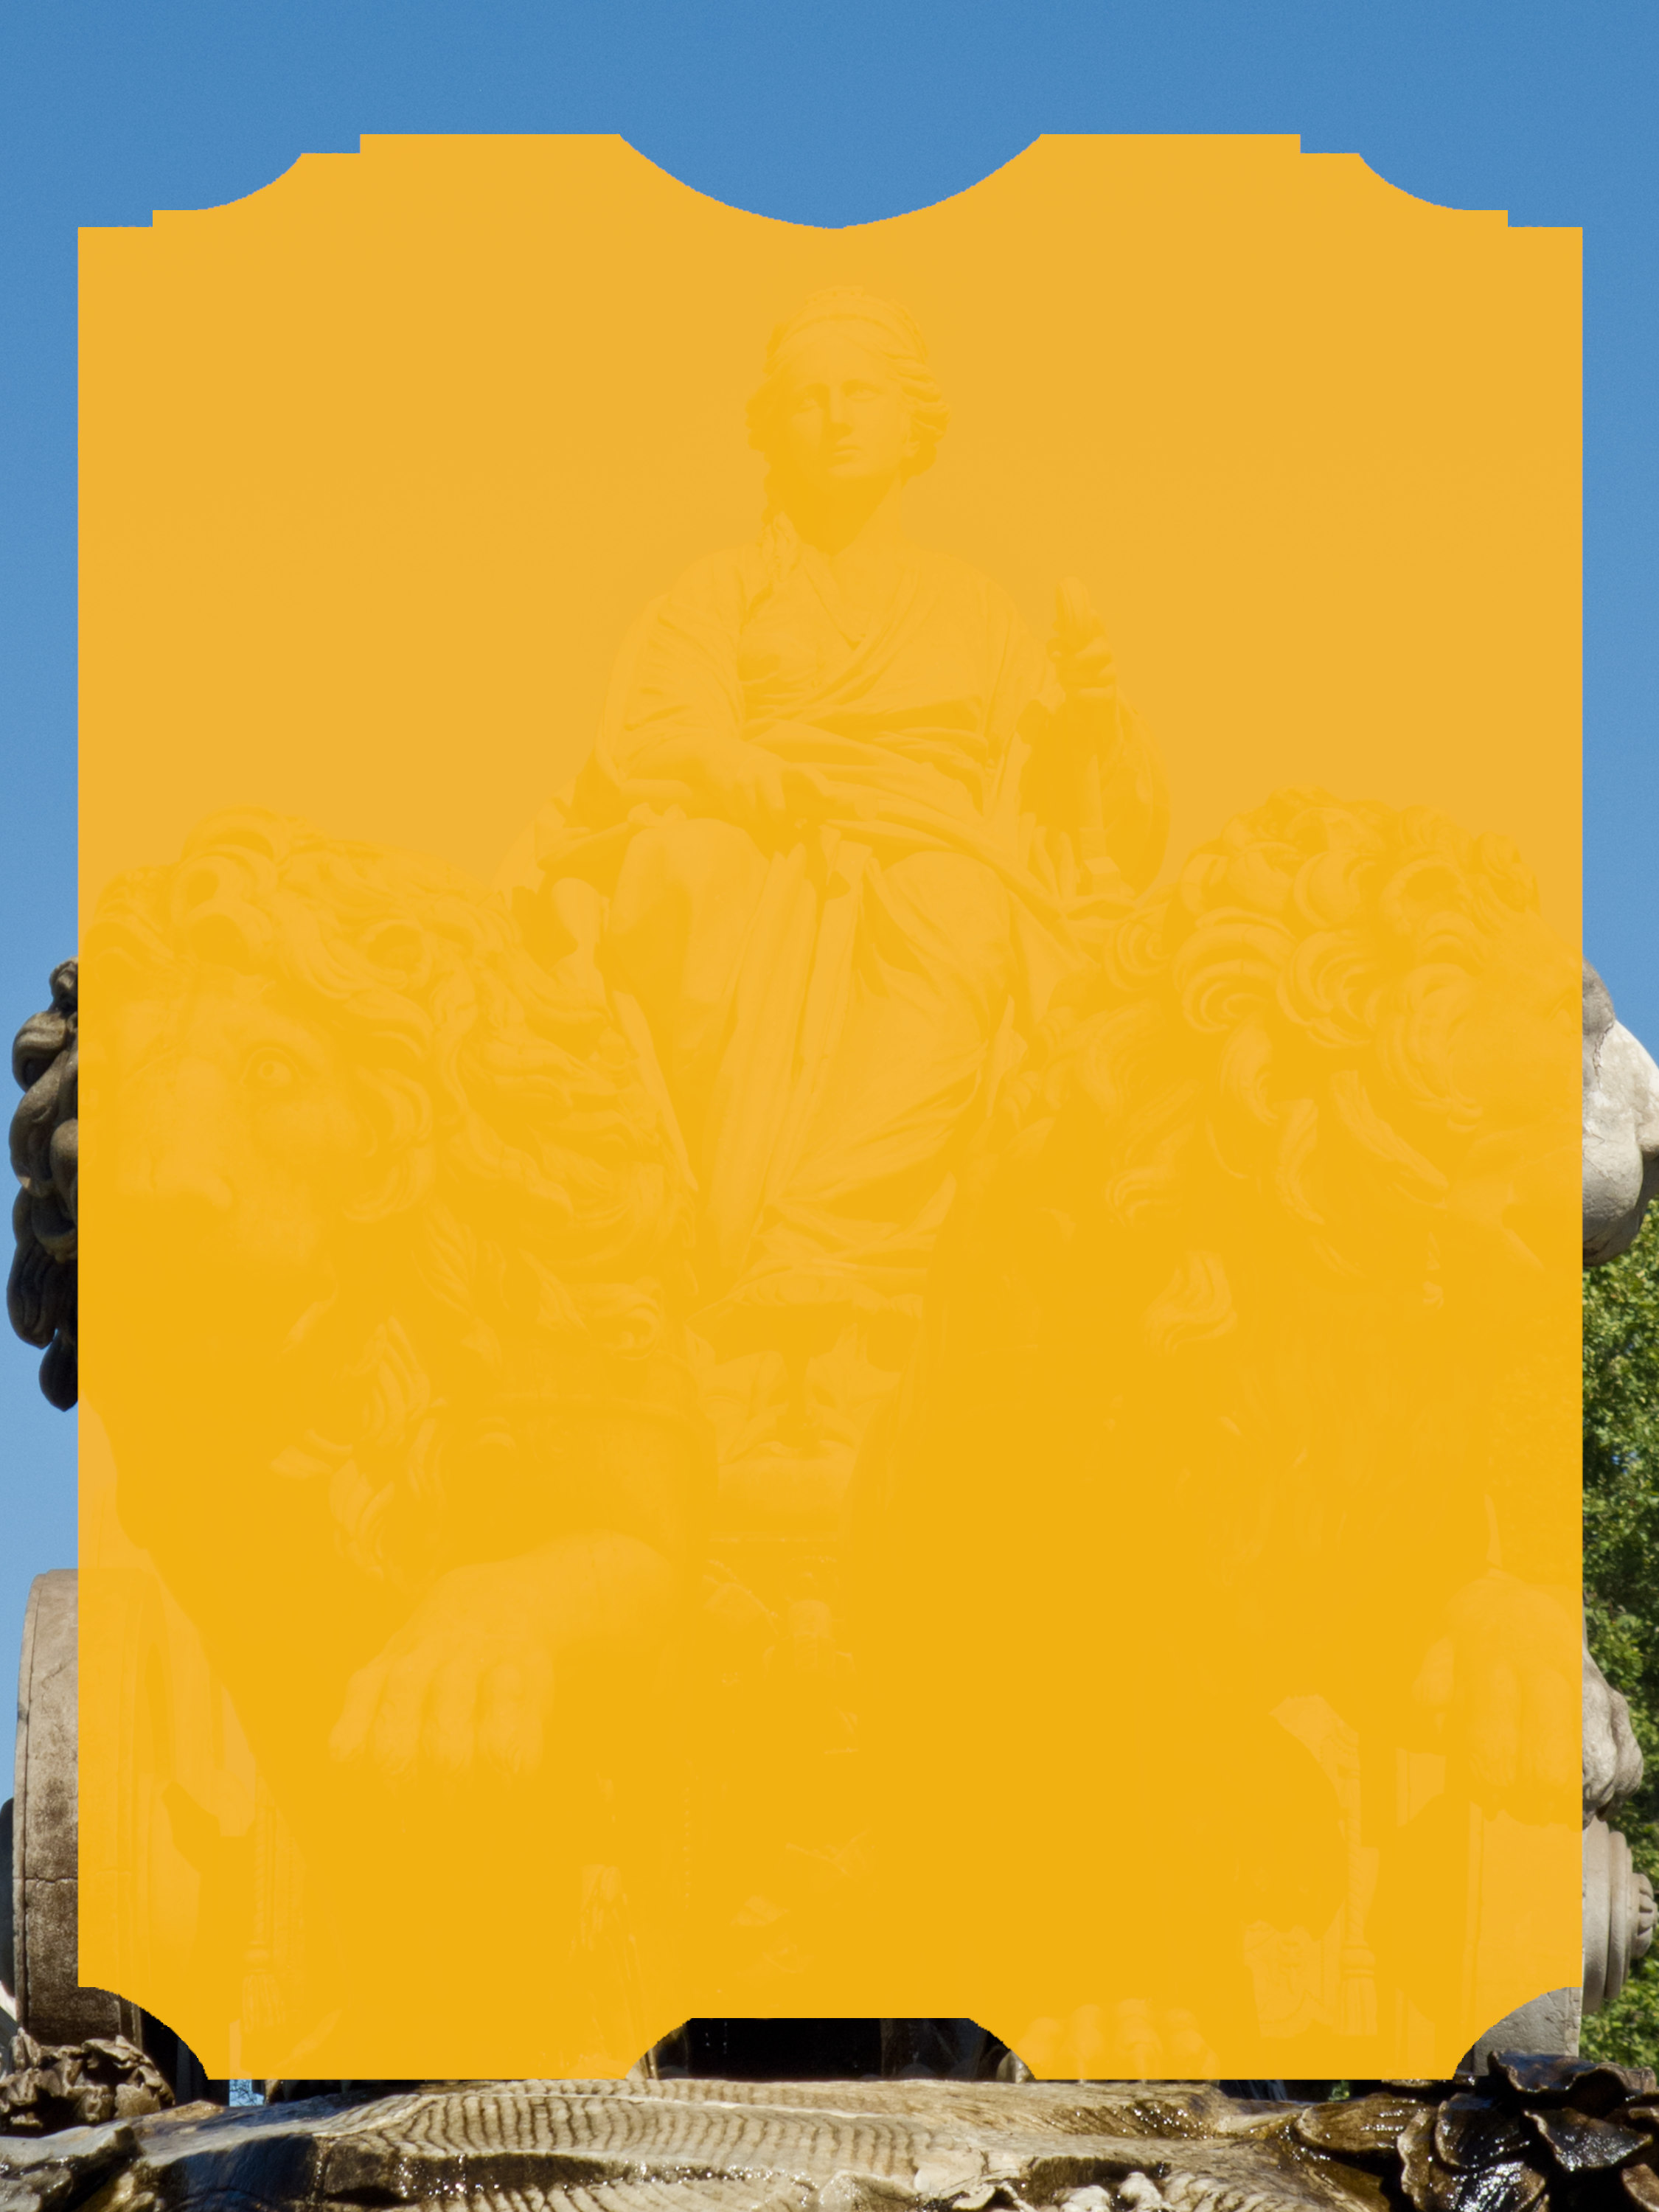
\includegraphics[width=\paperwidth,height=\paperheight]{cybele01.jpeg}}
\begin{titlepage} % Suppresses headers and footers on the title page
	\centering % Centre everything on the title page
	%\scshape % Use small caps for all text on the title page

	%------------------------------------------------
	%	Title
	%------------------------------------------------
	
	\rule{\textwidth}{1.6pt}\vspace*{-\baselineskip}\vspace*{2pt} % Thick horizontal rule
	\rule{\textwidth}{0.4pt} % Thin horizontal rule
	
	\vspace{1\baselineskip} % Whitespace above the title
	
	{\scshape\Huge Le Culte de Cybèle, \\Mère des Dieux, \\à Rome \\et dans \\l'Empire Romain}
	
	\vspace{1\baselineskip} % Whitespace above the title

	\rule{\textwidth}{0.4pt}\vspace*{-\baselineskip}\vspace{3.2pt} % Thin horizontal rule
	\rule{\textwidth}{1.6pt} % Thick horizontal rule
	
	\vspace{1\baselineskip} % Whitespace after the title block
	
	%------------------------------------------------
	%	Subtitle
	%------------------------------------------------
	
	{\scshape Par \Large Henri Graillot} % Subtitle or further description
	
	\vspace*{1\baselineskip} % Whitespace under the subtitle
	
        {\scshape\scriptsize Ancien Membre de l'École de Rome \\Maitre de Conférences a l'Université de Toulouse} % Subtitle or further description
    
	%------------------------------------------------
	%	Editor(s)
	%------------------------------------------------
        \vspace*{\fill}

	\vspace{1\baselineskip}

	{\small\scshape Paris 1912}
	
	{\small\scshape{Fontemoing et Cie, Éditeurs \\Libraires des Écoles françaises d'Athènes et de Rome, de l'Institut français d'Archéologie orientale du Caire, du Collège de France et de l'École Normale Supérieure \\4, Rue le Goff, 4}}
	
	\vspace{0.5\baselineskip} % Whitespace after the title block

        \scshape Internet Archive Online Edition  % Publication year
	
	{\scshape\small Utilisation non commerciale --- Partage dans les mêmes conditions 4.0 International} % Publisher
\end{titlepage}
\setlength{\parskip}{1mm plus1mm minus1mm}
\clearpage
\tableofcontents
\clearpage
\vspace*{\fill}
\begin{center}
A \\Monsieur Georges Perrot \\Ancien Directeur de l'École Normale Supérieure \\Secrétaire perpétuel de l'Académie des Inscriptions et Belles-Lettres \\\emph{Respectueux et affectueux hommage.}
\end{center}
\vspace*{\fill}
\clearpage

\section*{Préliminaires : Les Origines du Culte Métroaque.}
\begin{quote}
Τοῖς γὰρ ὁρθῶς εἰδόσι\\
τὰ θεῖα, μεῖζον Μητρὸς οὐχ ἔστιν ποτέ\\
ὅθεν ὁ πρῶτος οὐχ ἀπαιδεύτως ἔχων\\
ἱδρύσαθ᾽ ἱερὸν Μητρός.\\
Alexis.\footnote{Alexis de Thurium, poète comique (4\textsuperscript{e} s.). Dans Stob. \emph{Floriteg.}, 79, 13, èd. Meineke 1866, 3, p. 83.}
\end{quote}

Antiquité du culte d'une Grande Mère chthonienne, déesse des montagnes et souveraine des fauves, dans le bassin de la mer Égée et en Asie Mineure. --- 1. La Rhéa crétoise et préhellénique. Sa survivance dans les cultes helléniques. --- 2. La Kybelè anatolienne. Hittites, Phrygiens, Lydiens. La ville sacrée de Pessinonte et ses Attis. Expansion du culte phrygien en pays grec.

\subsection*{1.}

Une quinzaine de siècles avant notre ère, les Crétois adoraient une divinité féminine qui nous apparaît comme le prototype de Rhéa-Cybèle.\footnote{Sur la déesse crétoise, consulter en particulier : Evans, \emph{Mycenaean tree and pillar-cult}, dans \emph{Journal of Hell. St.}, 1901 ; \emph{Knossos excavations}, 1901-1903, dans \emph{British School Annual}, 7 (déesse aux lions, sur un pic, p. 29, fig. 9), 8, 9 (déesse en marche, accompagnée du lion, p. 59, fig. 37 ; dame aux serpents, p. 75, fig. 54) ; G. Karo, \emph{Altkretische Kultstaetten}, dans \emph{Archiv für Religionswissenschaft}, 7, 1904, p. 151 ss ; R. Dussaud, \emph{Questions mycéniennes} dans \emph{Rev. Hist. Religions}, 1905, et \emph{Fouilles récentes dans les Cyclades et en Crète}, dans \emph{Bult. et Mém. Soc. d'anthropologie de Paris}, 1906 ; Farnell, \emph{Cults of the greek States}, 3, 1907, p. 295 ss et pl. 33 ; H. Boyd Hawes, \emph{Gournia, Excavations 1901, 1903, 1904, publ. by the American Exploration Society}, 1908 (appendice A : Religion of the Minoans) ; Paribeni, \emph{Sarcofago dipinto di H. Triada} dans \emph{Monumenti antichi}, R. \emph{Accad. d. Lincei}, 29, 1908, p. 6-86 et 3 pl. ; Fr. von Dulin, \emph{Der Sarkophag aus H. Triada} dans \emph{Archiv f. Religionswiss.}, 1909 ; cf. Dussaud dans \emph{Rev. Hist. Religions}, 1908, 2, p. 365 ss, et A. J. Reinach, \emph{ibid.}, 1909, 2, p. 237 ss ; G. Karo dans \emph{Jahrbuch d. Inst.}, 1908, \emph{Arch. Anzeiger}, p. 122 s (fresque de Knossos avec scènes religieuses ; cf. Collignon dans \emph{Gaz. Beaux-Arts}, 1909, 2, p. 1-35). D'après la classification d'Evans, la troisième et dernière période du minoen, époque la plus brillante de la civilisation crétoise, correspondrait aux années 1800-1200, avec les subdivisions suivantes : 1, 1800-1600 ; 2 (époque des palais), 1600-1450 ; 3, 1450-1200. Après l'invasion achéenne (vers 1200), le minoen récent se continue par le mycénien ou achéo-égéen, qui dure jusqu'à l'invasion dorienne du 11\textsuperscript{e} siècle.} C'était la souveraine des montagnes. Lointaine et redoutable, elle réside sur les pics aigus, sur les cimes boisées, dans les profondeurs des grottes. Elle y est gardée par des lions. Quand elle parcourt ses domaines, un fauve l'accompagne. Déesse guerrière ou peut-être simplement chasseresse, elle brandit une arme, javeline, épieu ou double hache. On la figurait volontiers dans une attitude de combat. Mais elle est aussi la reine assise qui, une fleur à la main, reçoit les hommages et les actions de grâces de ses sujets. Car elle est bienveillante aux humains qui vivent sur son territoire et la révèrent selon les rites. Elle protège leurs foyers et leurs cités. On lui a réservé sa chapelle dans le palais de Knossos. Sur les portes des palais, sur les portes des villes, ses lions se dressent autour d'un pilier bétylique ou d'un autel, en signe de possession et de protection.

Au moment où la dame aux lions entre dans l'histoire, en plein âge du bronze, elle est le produit d'une évolution déjà longue. Avant de s'entourer de fauves, elle fut une bête fauve. Avant de se fixer sur la pointe des rochers, elle fut le rocher sacré. Avant d'être le pilier de pierre ou de bois, elle avait été la pierre brute ou l'arbre feuillu. Longtemps même, à côté de l'image anthropomorphe, subsista ce type intermédiaire du pilier aniconique. Le totémisme primitif laissait de très nombreuses survivances. Ses traditions singulièrement tenaces vont se prolonger au-delà de l'ère mycénienne. Mais, dès la période finale du minoen, dans la religion naturaliste qui s'édifie sur les bases du polydémonisme, les antiques fétiches se groupent autour de quelques divinités supérieures. La plus importante paraît être la Terre, considérée dans ses forces productrices, principe féminin de vie, déesse de fécondité et de fertilité, mère et nourricière de tout ce qui naît et meurt ici-bas. « La terre fait sortir les fruits du sol, » chantaient d'après un vieil hymne les prêtresses de Dodone ; « appelons donc la Terre du nom de Mère.\footnote{Paus. 10, 12, 10. Sophocle, \emph{Philoct.} 391 ss, appelle Ga la déesse des montagnes, dame aux lions, qu'il identifie à Rhéa, mère de Zeus, et à la Kybêbè de Sardes. Dieterich, \emph{Mutter Erde} dans \emph{Archiv f. Relig.}, 1905, p. 1 ss.} » C'est elle que l'on adore sur les montagnes, qui sont ses trônes, dans les cavernes, qui sont ses premiers temples, dans les bois et près des sources, manifestations de sa mystérieuse et bienfaisante énergie. Pour la distinguer des mères topiques,\footnote{Il y avait un culte très ancien des « Meteres » crétoises : Diod. Sic. 4, 80, ce qui prouve bien l'importance de cette idée de maternité dans la religion minoenne. Ces Mères sont appelées aussi Nymphes, cf. Timée, \emph{Frg.} 83.} représentant les esprits d'un lieu déterminé, multiples génies de la roche, de l'antre, de l'arbre ou de l'eau, on dut lui attribuer le titre de Grande Mère très anciennement.\footnote{Le vocable de Megalé Meter apparaît seul sur des dédicaces de Phaestos, en Crète (époque hellénistique), \emph{Museo Italiano}, 3, p. 736 ; cf. \emph{Ath. Mitth.}, 1893, p. 272 ; 1894, p. 290 ; de Delos, \emph{Bull. Corr. Hell.}, 1882, p. 500, n° 25 ; de Thespies, \emph{CIG Sept.} 1, 1811 ; de Sparte, Paus. 3, 12, 9 ; cf. Pind., \emph{Fragm.} 48 et 63 (Boeck).} Elle portait aussi le nom de Rhéa, dont nous ignorons la signification primordiale et qui s'est conservé dans les cultes grecs.\footnote{Voici, à titre de curiosité, quelques-unes des étymologies proposées. Les anciens rapprochaient le mot Rhéa du verbe ῾ρεῖν, couler ; Gruppe, \emph{Griech. Mythol. und Religions Gesch.}, 1906, p. 1524 s, y voit le nom d'une pierre-fétiche, que l'on aurait adorée pour obtenir la pluie, cf. lapis manalis. D'autres voyaient dans Rhéa une métathèse d'Era = Terre : Eustath., \emph{Ad Iliad.}, 1, 55 ; \emph{Reinesius, Syntagma inscr. antiq.}, 1682, p. 73 ; Welcker, \emph{Griech. Goetterlehre}, 2, 216 ; Buchholz, \emph{Homer. Realien}, 3, 1, p. 11 ; Decharme dans Daremberg et Saglio, \emph{Dict. des Antiq.}, s. v. \emph{Cybelé}. Crusius, \emph{Beitr. z. griech. Mythol.}, Leipz. Progr., 1886, p. 26, n. 4, suppose Rhéa (Rheia dans Homère et Hésiode) = O]reia ; cf. Sonny dans \emph{Philologus}, 1889, p. 559, Dieterich, \emph{ibid.}, 1894, p. 5, et Immisch dans Roscher, \emph{Myth. Lex.}, 2, 1613. Les sémitisants rapprochent Rhéa de Raiah = amie, aimée, compagne : Assmann, \emph{Vorgeschichte von Krela}, dans \emph{Philologus}, 1908, p. 177, qui croit encore à l'hypothèse phénicienne, démentie par les fouilles récentes.} C'est elle que l'on conçoit comme la dompteuse des fauves, terribles hôtes des montagnes et des forêts. Sans doute n'y eut-il à l'origine, dans cette conception du rôle divin, qu'une raison de pure magie. En lui soumettant les animaux dont on redoutait le pouvoir destructeur, l'homme pensait assurer contre le danger sa personne, ses troupeaux et sa maison. Mais c'est elle encore qui se révèle comme charmeuse de serpents. Dame aux lions et dame aux reptiles, rapprochées déjà dans les chapelles palatines de Knossos, tendent à confondre leur individualité, à réunir leurs attributs. Le serpent qui sort des crevasses du sol vient s'enrouler à la base des piliers-bétyles. Car il est le génie du monde souterrain ; et la déesse chthonienne étend à la fois son empire sur la terre et dessous. Celle-ci, d'autre part, est en relations avec le monde aérien. Sur le pilier d'abord, puis sur la tête ou sur les mains de l'idole, nous voyons se poser familièrement certains oiseaux sacrés. Ils sont devenus ses messagers célestes. La déesse de la terre est en effet associée à un dieu du ciel, dieu des phénomènes atmosphériques entre ciel et terre, dont les Grecs feront un Zeus. Maître de la foudre et des tempêtes, c'est un guerrier armé de la lance, le plus souvent de la bipenne, et du bouclier bilobé ; sa coiffure est un casque ou bonnet pointu. Quand il agite son bouclier de bronze et brandit sa double hache, il produit orages et pluies. Dans les sanctuaires minoens, le dieu mâle est encore représenté par ces fétiches skeuomorphes. Son culte reste lié, de même, à celui de certains animaux. Peu à peu s'absorbe en lui la personnalité de l'ancien dieu taureau, dont plusieurs légendes amoureuses caractérisent la puissance génésique\footnote{Légendes d'Europe, de Pasiphaé. Cf. Cook, \emph{Animal worship in the mycenaean age}, dans \emph{J. of Hell. St.}, 14, 1894, p. 120-132 : The cult of the bull.} ; le taureau devient son attribut. Dieu qui féconde la terre, son culte est lié aussi à celui des arbres. On dresse la bipenne sur un pilier de bois, souvent garni de feuillages ; à Dodone, on l'enfonçait dans le chêne de Zeus. Plus tard, c'est le dieu lui-même que l'on figure assis sur un tronc d'arbre et entouré de plantes. Tel il nous apparaît sur les monnaies de Phaestos, dont le revers porte l'effigie taurine. Parmi les arbres sacrés, il y a plus spécialement ceux qui demeurent toujours verts : pins et cyprès, surtout oliviers et palmiers,\footnote{Cf. Paribeni, l. c., p. 29 et 42. Rhéa possédait à Knossos son bois de cyprès : Diod., 10, S6. Von Duhn croit que, sur le sarcophage d'Haghia Triada, les piliers sont de petits obélisques en bois, recouverts de feuilles de cyprès. Il y avait à Gortyne un platane sacré dont les feuilles étaient persistantes (sans doute un sycomore) : Theophr., \emph{Hist. plant.} 1, 15.} dont les fruits sont précieux à l'homme. Ils deviendront facilement des symboles d'immortalité et prendront une signification funéraire, s'ils ne l'ont déjà. Le dieu, fils de Rhéa qui est la Terre Mère, né dans une caverne comme beaucoup de dieux lumineux, meurt en pleine jeunesse, comme les dieux solaires et agraires\footnote{Cf. Déchelette, \emph{Le culte du soleil aux temps préhistoriques dans Rev. archéol.}, 1909, 1, p. 357 : « comme les primitifs attribuaient une origine commune à l'éclair et aux rayons du soleil, le dieu de la foudre se trouve étroitement apparenté aux divinités du cycle solaire. »} ; on montrait sa tombe à Knossos. Bien des éléments intervinrent dans la constitution progressive de ces deux personnalités divines. Il convient d'y faire une part, sans doute importante, aux influences égyptiennes et chaldéo-élamites ; ces dernières se seraient exercées sur le monde égéen par l'intermédiaire de la Syrie. Les divinités chthoniennes et célestes de l'Égypte et de la Chaldée, où se multiplient déesses lionnes et déesses serpents, dieux taureaux et dieux à la hache, ont pu faire sentir leur action sur les divinités similaires de Crète, en modifier ou en agrandir le concept. Beaucoup de ces déesses sont, comme Rhéa, les dames de la montagne : telles l'égyptienne Hathor, dont le serpent s'associe au lion solaire de Râ, et la babylonienne Ninhursag, toutes deux « mères et nourricières des rois\footnote{Sur les frappantes analogies de ces deux divinités, d'après les textes et les monuments figurés, v. A. Boissier dans \emph{Oriental. Litteraturzeitung}, 11, col. 234-236. Influence du culte d'Hathor sur l'iconographie de la Meter dans l'art cypro-mycénien : Evans, \emph{Mycenaean tree and pillar-cult}, p. 69 ; l'auteur voit en particulier dans la couronne murale de la déesse anatolienne « un dérivé direct de la maison de Hor sur la tête d'Hathor » ; mais il y a plutôt ici une influence immédiate de l'art babylonien.} » ; telle Ishtar-Nana, qui debout sur un léopard ou un lion,\footnote{Cf. Maspero, \emph{Hist. anc. des peuples de l'Orient}, 1, p. 681. Le disque étoilé d'Ishtar se retrouve sur un anneau d'or de Mycènes.} couronnée de tours et armée de l'arc, parcourt monts et vaux en criant : « je suis reine dans le combat » ; telles enfin la plupart des Beltis syriennes, debout aussi sur un fauve, les mains pleines de serpents et de fleurs. Certaines ne sont connues que sous leur vocable de Mères : la Moût léontocéphale de Thèbes, par exemple, et Mami, qui est une hypostase d'Ishtar, la Terre qui reverdit au printemps.\footnote{Ces divinités ne sont pas plus en Égypte et en Chaldée qu'en Crète des personnes abstraites, qui président métaphysiquement aux forces de la nature. Chacune enferme en soi l'un des éléments de l'univers et est la matière même de cet élément avant d'en devenir l'esprit ; elle continue à y résider alors même que le progrès religieux l'en a isolée.} Il en est même qui sont déjà qualifiées de Mères des Dieux ; telles la Nana d'Ourouk et la Baou de Sirpourla, déification de la Terre maternelle, productrice de vie et protectrice des fruits de la vie, épouse d'un dieu solaire et guerrier. Mais ces divinités féminines ne sont que les égales des dieux parèdres, et souvent leur sont inférieures.\footnote{En Égypte règne l'égalité entre les dieux et les déesses, qui participent à l'exercice du pouvoir suprême : cf, Maspero, l. c., p. 101. 11 semble au contraire que les déesses babyloniennes aient en général un caractère passif et presque impersonnel.} Ce qui distingue la Mère ou peut-être Vierge Mère\footnote{Farnell, l. c., p. 305 s. ; cf. en Asie-Mineure, Ramsay, \emph{Cities and bishoprics of Phrygia}, 1895-97, 1, p. 136.} crétoise, c'est sa suprématie. Dans la religion égéenne prédomine l'aspect féminin de la divinité. Tradition héritée d'un ancien état social, où la toute-puissance du sang maternel était la loi ? Le matriarcat, régime de peuples arriérés, survivait encore en Lycie au temps d'Hérodote ; il n'avait pas encore complètement disparu de la civilisation étrusque, et l'on croit en retrouver le souvenir dans quelques coutumes des Ligures.\footnote{Références dans Paribeni, Z. c., p. 81. Pour les Ligures, cf. Jullian, \emph{Hist. de la Gaule}, 1, 1908, p. 178. Le mythe pessinontien d'Agdistis nous en offre peut-être un exemple en Phrygie : Agdistis porte un nom dérivé de celui de sa mère, la roche Agdos, fécondée par Zeus ; la filiation s'établit de la mère à l'enfant.} A la hiérarchie divine correspond la hiérarchie sacerdotale. Les femmes y occupent le premier rang ; c'est à elles que sont dévolues les principales fonctions de la liturgie. Le rôle des hommes paraît n'être qui accessoire.\footnote{Citharède, flûtiste, porteurs, sur le sarcophage d'Haghia Triada.} Aussi bien, d'une façon générale, les hommes ne sont-ils pas admis dans l'enceinte du temenos.\footnote{Fresque de Knossos ; cf. A. J. Reinach, \emph{l. c.}, p. 243.} Le culte est orgiastique. Il comporte des danses sacrées, au son de la lyre et de la double flûte qui accompagnent aussi les sacrifices. Les unes sont exécutées par des femmes. Les autres sont des danses d'hommes armés ; elles ont donné naissance au mythe des Curètes Idéens. Suivant un rite familier aux peuplades primitives, ces guerriers entrechoquent bruyamment leurs boucliers et leurs glaives\footnote{A l'origine, leur double hache ; cf. le Curète Labrandos (λάβρυς, hache) et les rapprochements proposés par Eisler, \emph{Kuba-Kybele} dans \emph{Philologus}, 68, 1909, p. 126, n. 27.} soit pour conjurer le tonnerre, soit pour évoquer la pluie et pour aider à la renaissance annuelle de la nature.\footnote{Les danses armées des Saliens, à Rome, avaient sans doute la même origine ; cf. Salmoneus, roi légendaire de Thessalie, imitant le tonnerre en faisant résonner une cuve de bronze. Sur le caractère prophylactique et apotropaïque du bronze, v. Cook, \emph{The gong of Dodona} dans \emph{J. of Hell. St.}, 22, 1902, p. 14 ss.}

L'orgiasme conduit à l'extase. De plus, la mantique est un élément ordinaire des cultes chthoniens. La déesse crétoise semble avoir eu ses prophètes ou prophétesses. Mais, par l'orgiasme, c'est toute une tribu ou tout un peuple qui participe à la communion divine. Chaque année, pour bénéficier des vertus de l'arbre divin, on le met en pièces et l'on s'en partage les débris.\footnote{Des gemmes nous montrent l'olivier violemment secoué ou même arraché ; cf. la légende thessalienne d'Erysichtôn détruisant le bois sacré de Demeter, « mauvaise explication du rite primitif » : A. J. Reinach, \emph{l. c.}, p. 240.} Certains sacrifices d'animaux sacrés, taureaux et bouquetins, s'accomplissaient probablement selon le même rite, que nous retrouvons chez les Thraces.\footnote{On a cherché dans la légende des amours de Pasiphaè le souvenir dégradé d'une communion mystique avec le dieu taureau : Dieterich, \emph{Eine Mithras Liturgie}, p. 136 ; Farnell, \emph{l. c.}, p. 297.} Peut-être usait-on du taurobole, qui est à l'origine un rite magique. Ne serait-ce pas aussi d'une pratique baptismale, faisant renaître à une vie nouvelle, que dérive la légende de Pélops, régénéré par les soins de Rhéa\footnote{Farnell, \emph{ibid.}} ? Les Minoens enfin croient à une survie d'outre-tombe. La déesse mère et le dieu fils, qui a subi la mort et qui l'a vaincue, étendent sur cet autre monde leur suzeraineté. Ils continuent à y protéger leurs féaux d'ici-bas. Donc il faut les propitier pour le trépassé, parti sur une barque. Grâce aux prières et aux sacrifices, celui-ci achève son voyage dans un bige de griffons ailés, que conduit une déesse psychopompe et qui l'emporte au divin séjour.\footnote{Paribeni, \emph{l. c.}, p. 24 s, 59 s, 77 ss. La barque rappelle l'Égypte. Les Babyloniens semblent avoir eu l'idée de morts voyageant en char : A. J. Reinach, \emph{l. c.}, p. 241.} Un lien étroit unit le rituel funéraire au culte des grands dieux. Le tombeau du mort héroïsé s'associe à l'autel, aux emblèmes de la divinité, aux arbres sacrés.

Cette religion n'était point particulière aux Eteocrètes. Elle semble avoir été commune à toutes les populations de même race, ou de même civilisation, qui habitaient le continent grec, les îles égéennes et l'Asie Mineure. C'était la religion des Pélasges. Après l'invasion dorienne, elle se survit à elle-même dans le sanctuaire de Dodone ; mais à Delphes Apollon Pythios et Pythoktonos, dieu serpent devenu le tueur du serpent, se substitue à la pélasgique Gaia. Sous le vocable de Rhéa, la dame des montagnes entre dans le panthéon hellénique. Elle figure au vie siècle sur une inscription d'Ithaque,\footnote{Entre Héra et Athéna. Roehl, \emph{Inscr. graec. ant.}, 336.} au ive sur une inscription de Cos.\footnote{Paton et Hicks, \emph{Inscr. of Cos}, 1891, n° 38.} Athènes lui a dédié un sanctuaire dans le temenos de Zeus Olympios. Son culte se maintient surtout dans le Péloponèse, où l'influence crétoise fut très active, et particulièrement dans le massif d'Arcadie, où persistent les vieilles traditions.\footnote{Cf. Farnell, \emph{l. c.}, p. 294, n. \emph{e.} Sur le culte de Rhéa en Arcadie, cf. Immerwahr, \emph{Rhea Sage und Rhea Kult in Arkadien} dans \emph{Bonner Studien für Kekulé}, 1890, p. 188-193, et \emph{Die Kulte und Mythen Arkad.}, 1, p. 213 ss.} A Phigalie, à Tégée, le mythe de Rhéa est populaire comme une tradition nationale.\footnote{Paus. 8, 41, 2 ; 47, 3.} Les Arcadiens localisent au mont Lykaion l'enfantement de Zeus,\footnote{Callim., \emph{Hymn. in Jov.}, 10.} adorent aussi Rhéa dans une grotte du mont Thaumasion, où seules ses prêtresses ont le droit de pénétrer,\footnote{Paus. 8, 36, 3.} et lui associent Zeus sur le mont Azan, « ritu Idaeo.\footnote{Lact. Plac., ad Stat., \emph{Theb.} 4, 292.} » Dans la vallée de l'Alphée elle conserva longtemps ses prophétesses.\footnote{Dio. Chrys., \emph{Or.}, p. 59 s.} A Olympie, elle occupait tout d'abord auprès de Zeus une situation éminente.\footnote{Cymbales de bronze, consacrées dans le temple de Zeus, mais qui étaient associées sans doute au rituel de la Meter : \emph{Bronzen v. Olympia}, texte, p. 70.} A Messène, à Epidaure, à Lycosura, comme à Olympie même, son origine préhellénique est attestée par la présence des Curètes crétois, des Dactyles Idéens et de l'Idéen Héraclès.\footnote{Paus. 4, 36, 6 (Messenia, statue de la mère des dieux) et 9 (megaron des Curètes, temple d'Eileithyia) ; 5, 8, 1 (Dactyles Idéens et Curètes à Olympie), 8, 37, 2 (naos de Demeter, autel de la Megale Meter à Lykosura) et 3 (Curètes, Corybantes) ; Cavvadias, \emph{Fouilles d'Epidaure}, n°\textsuperscript{s} 40 (autel des Curètes), 64 (dédicace à Megale Meter Theôn) ; cf. Demeter et Héraclès, considéré comme l'un des Dactyles Idéens, à Megalopolis et à Mycalessos : Paus. 8, 31, 3 ; 9, 19, 5.} Enfin au Metrôon d'Akriai, dressé sur un promontoire de Laconie, cette origine est attestée à la fois par une légende, relative à la très haute antiquité du temple, et par les nombreux vestiges que la religion crétoise a laissés dans le pays.\footnote{Paus. 3, 22, 4. Cultes de Britomartis, de Pasiphaé, d'Apollon Delphinios dans le sud de la Laconie. Farnell, \emph{l. c.}, p. 294, n. \emph{a.}} Mais, en s'hellénisant, la déesse peu à peu se dépouille de ses caractères orgiastiques. Par contre, à mesure que se constitue la théogonie nouvelle, la notion de sa maternité divine s'amplifie. A l'époque homérique, la mère de Zeus est devenue également celle de Poséidon, Hadès et Héra. L'auteur de la \emph{Théogonie} dite hésiodique, au 8\textsuperscript{e} siècle, ajoute Hestia et Demeter. C'est entre le 8\textsuperscript{e} et 6\textsuperscript{e} vie siècles, dans un fragment d'hymne, que nous voyons apparaître une « Mère de tous les Dieux,\footnote{\emph{Hymn. hom.} 14, 1 ss. Sur l'importance de ce titre de Mère des dieux, qui implique un dogme et tout un système religieux, cf. Farnell, \emph{l. c.}, p. 291.} » principe de toute vie divine et humaine. Pour la première fois, ce titre de Mère des Dieux est présenté comme un vocable personnel, qui se suffît à lui-même. La divinité qu'il désigne passe pour habiter « les montagnes aux échos sonores et les ravins boisés, » en compagnie des loups et des lions. Elle est donc l'un des aspects de Rhéa. La littérature du Ve siècle n'a pas tort de confondre les deux déesses.\footnote{« The primary question must be first discussed whether this identification of Rhea with the Θεῶν Μήτηρ of the Greek mainland is an original fact explaining the religious dogma expressed by the title, or whether it is one of those later syncretisms so common in all polytheistic religions. » Farnell, \emph{l. c.}, p. 293. Rapp, dans Roscher, \emph{Myth. Lex.}, 2, p. 1660, s. v. Kybele, tend à distinguer la Mère des Dieux hellénique et la Rhéa Cybèle crétophrygienne. Farnell, qui tire parti des découvertes crétoises, défend la première hypothèse.} La religion toutefois les distingue. Avec deux appellations différentes, une même divinité se dédouble et exige deux autels ; les mots peuvent créer des dieux. A vrai dire, dans la Grèce classique, Rhéa est une divinité déchue, comme son époux et parèdre Chronos. Elle fut supplantée par la Mère des Dieux, dont le culte restait en communication plus intime avec la vie de la terre, des sources et des arbres.\footnote{Sur les monuments figurés, la M. d. D. est souvent unie aux Nymphes, à un dieu fleuve et à Pan.} Dans cette expansion d'un culte au détriment d'un autre, quelle est la part des influences extérieures ? D'après une tradition athénienne, la Mêter serait une importation de l'Anatolie ; et son culte officiel en Attique ne daterait que du 5\textsuperscript{e} siècle.\footnote{Julian., \emph{Or.} 5, p. 159 AB ; Suid., s. v. Metragyrtes ; Phot., s. v. Metrôon ; Schol. in Aristoph., \emph{Plut.} 431 ; cf. Hepding, \emph{Attis}, 1903, p. 135. Par contre, sur l'hypothèse qui rattache le nom même de l'Attique à un culte préhistorique d'Attis, cf. Eisler, \emph{l. c.}, p. 166, n. 149.} La tradition se manifeste, il est vrai, sous les apparences d'une légende. Signalée seulement à la fin du paganisme, elle est sans valeur historique ; c'est une forme tardive du mirage oriental. Mais on ne saurait mer toute influence de l'Asie Mineure, où la Grande Mère avait conservé sa suprématie.

\subsection*{2.}

Vers l'an 1500, selon la chronique de Paros, aurait eu lieu sur les monts Kybèles, dans le pays qui devint beaucoup plus tard la Phrygie, une miraculeuse apparition de la Mère des Dieux.\footnote{\emph{CIG.} 2374, l. 19.} En Asie Mineure comme en Crète, la Grande Mère, Mâ, était au premier rang des divinités indigènes. Elle régnait sur les montagnes, dont les forêts de pins lui sont consacrées, sur les plateaux aux sources rares et aux maigres pâturages, sur les plaines fertiles. Les plus anciens sanctuaires que nous lui connaissons se dressent au bord de fontaines et d'étangs.\footnote{A Boghaz-Koï (Cappadoce), Ibriz et Efflatum-Bunar (Lycaonie). Dans ces deux dernières localités, l'image regarde la source, qui lui baigne le pied : cf. Sarre, \emph{Reise in Phrygien} dans \emph{Arch. ep. Mitt.}, 1896, 19, p. 40 ss ; Reber, \emph{Die Phryg. Felsendenkm.}, 1897, p. 4 s. Au mont Sipyle, près de l'image de la Meter Plasténè, taillée aussi dans le roc, petit lac « fed by countless springs that gush from the rocky foot of the mountain » : Frazer, à Paus. 5, 13, 7, \emph{Comment.}, 3, p. 554 (bibliogr., p. 555 s) ; c'est probablement l'ancien lac Saloe.} Ses plus anciennes images sont taillées dans la roche vive. Le lion est près d'elle ou sous ses pieds ; à Iasili-Kaïa, en Ptérie, son effigie humaine n'est même pas encore complètement dégagée du type léontomorphe.\footnote{Perrot et Chipiez, \emph{Hist. de l'art dans l'antiq.}, 4, fig. 320, p. 647. Sur le lion en Asie Min., cf. Otto Keller, \emph{Die antike Tierwelt}, 1, 1909, p. 24-61.} La déesse mère est associée à un dieu jeune, imberbe,\footnote{Perrot et Ch., \emph{ibid.}, p. 650 s ; 5, p. 216 (Iasili-Kaïa) ; Ramsay dans \emph{Ath. Mitth.}, 14, 1889, p. 172 (Fassiler).} qui est un dieu lumineux, et que l'on nomme Attis ou Atès.\footnote{Ramsay, \emph{Cities}, 1, p. 132 et 169. Le nom apparaît pour la première fois sous la forme \emph{Ates} (monument de Midas, cf. Perrot et Ch., \emph{op. l.}, 5, p. 82-89 et fig. 48). Démosthène, \emph{Pro Cor.}, 260, donne la forme Ἄττης, qui est aussi dans Hermesianax (cf. Paus. 7, 17) et Nicander, \emph{Alexipharm.}, 8 et schol. ; même forme rituelle du nom à Pessinonte, Paus. 1, 4, 5, à Dymé et Patras, au 2\textsuperscript{e} s. de notre ère, Paus. 7, 17, 9 et 20, 3. Ἄτυς nom théophore dans les dynasties royales de Lydie, Hérodot. 1, 34 ; nom d'un prêtre de Cybèle dans Dioscorides, \emph{Anth. Pal.}, 6, 220 (Ἄτις potius quam Ἄτυς cod. ante rasuram). Ἄττις, dans le poète comique Theopompe, contemporain d'Aristophane : \emph{Fragm. Comic. Gr.}, éd. Meineke, 2, p. 801 ; \emph{Com. Att. fragm.}, éd. Kock, 1, p. 740. La consonne est redoublée dans les noms de plusieurs villes d'Anatolie, qui paraissent dérivés de celui du dieu, Attaia, Attouda, etc. Parmi les différentes étymologies que l'on a cherchées, cf. Arnob. 5, 6 : Attis = scitulus, mignon, en Lydie. Attis = Adôn, seigneur : Haakh dans \emph{Stuttgart. Philol. Versamml.}, 1857, p. 176 s ; Tomaschek dans \emph{Ak. Wien. Sitzungsber.}, 130, 1894, p. 42 ; cf. Eisler, \emph{l. c.}, p. 178, n. 176. Attis, contraction d'Agdistis = fils de la montagne : Ramsay dans \emph{J. of. Hell. St.}, 3, 1882, p. 56. Attis = père : Vanicek, \emph{Fremdwoerter im gr. und lat.}, 1878, s. v. Ἄττης ; Kretschmer, \emph{Einleitung in die Gesch. d. gr. Sprache}, 1896, p. 350 ss (avec les diverses formes du nom) ; Gruppe, \emph{Gr. Mythol.}, 1906, p. 1548.} Ce dieu est son fils. C'est pourquoi, dans la période d'expansion hellénique, Meter Lêto et Apollon pourront si facilement se substituer au couple primitif.\footnote{Ramsay, \emph{op. l.}, p. 6 s, 130 s, 146, 192, 264, 305.} Nombreux et variés sont les souvenirs d'anciens cultes, qui se rattachent à la même religion que ceux de la Crète minoenne et de la Grèce mycénienne. En Lydie, un mythe situe sur le Tmolos la retraite de Rhéa et la naissance d'un Zeus Hyetios, seigneur de la pluie, gardé par les Curètes.\footnote{\emph{Anthol. Pal.}, 4, p. 511 ; Lyd., \emph{De mens.} 10, 71 (48) ; cf. Hyes Attes dans Demosth., \emph{l. c.}, et Jupiter \emph{Pluvialis}, \emph{CIL.} 9, 324 ou \emph{Pluvius}, Tib. 1, 7, 26 ; Usener, \emph{Goetternamen}, 1896, p. 46 s ; Farnell, \emph{op. l.}, 5, p. 124 s.} Dans la région du Sipyle, on montrait l'emplacement de deux villes disparues, qui furent Sipylos Idaia et la forteresse des Curètes.\footnote{Strab. 1, 3, 17 et 12, 8, 21 ; Plin., \emph{H. n.} 5, 29.} A Éphèse, le culte des Curètes est associé à celui d'Artémis-Lêto.\footnote{Strab. 14, 1, 20, p. 640 ; cf. en Carie le culte de Zeus Cretagénès et des Curètes : Lebas-Waddington, \emph{Inscr.}, 5, 338, 394 et 496.} En Mysie, la Meter de Cyzique a pour acolytes les Dactyles Idéens crétois.\footnote{Apoll. Rh., \emph{Argon.} 1, 1, 1125-29 et Schol., qui signale la même association de Rhéa et des Δάκτυλοι Ἰδαῖοι Κρηταιέες.} Et l'Ida troyen rappelle les liens antiques de l'Asie Mineure avec la Crète, qui remontent au temps de l'hégémonie crétoise sur le bassin de l'Égée.\footnote{Sur les rapports primitifs de la Crète et de la Phrygie, cf. Ramsay, \emph{Cities}, 1, pp. 94 et 358 ; Gruppe, \emph{op. l.}, p. 301 : Farnell, \emph{op. l.}, 4, p. 165 s. Une tradition faisait remonter à l'Arcadien ou Crétois Dardanos et à son fils Idaios l'introduction du culte métroaque dans la région de l'Ida troyen : Dion. Hal. 1, 61 ; Diod. Sic., 5, 49.}

Plusieurs des monuments où figure soit le couple divin, soit la seule déesse, sont d'origine hétéenne, par conséquent antérieurs au 11\textsuperscript{e} siècle. A l'époque indiquée par les marbres pariens, les Hittites, descendus probablement du massif du Taurus,\footnote{Cf. de Morgan, \emph{Les premières civilisations}, 1909, p. 281.} étendaient leur domination de l'Euphrate à la Méditerranée et à la mer Noire. Leurs princes traitaient d'égaux à égaux avec les rois de Babylone et les Pharaons d'Égypte, maîtres de la Phénicie et de la Syrie méridionale. Ce peuple a subi, dans ses conceptions religieuses, le double ascendant de l'Égypte et de la Babylonie\footnote{Ramsay, dans \emph{Ath. Mitth.}, 14, 1889, p. 175 ss, croit retrouver des influences assyriennes sur les monuments d'Ibriz, égyptiennes sur ceux de Ptérie ; cf. Sarre, \emph{l. c.}, et Reber, \emph{op. l.}, p. 3 ss, 18-24 (infl. mésopotamiennes sur la tombe dite des lions, Arslantasch, en Phrygie, 8\textsuperscript{e} siècle ? ).} ; et les éléments de la civilisation qu'il apporte aux grossières tribus de l'Anatolie occidentale, c'est surtout aux Chaldéo-Babyloniens qu'il les emprunte. La pénétration profonde du sémitisme est donc antérieure aux deux invasions assyriennes, qui datent des 11\textsuperscript{e} et 9\textsuperscript{e} siècles. Au moment même où le monde mycénien s'écroule sous la poussée dorienne, nous voyons se consommer la ruine de l'empire hétéen. Mais l'influence sémitique est entretenue, à l'intérieur, par l'établissement définitif des Syriens Blancs sur la rive droite de l'Halys et, dans les régions côtières, par l'extension du commerce phénicien ; elle se renouvelle au 3\textsuperscript{e} siècle par la fondation de colonies séleucides en Lydie et en Phrygie. Elle s'était exercée sur les rites et sur le mythe. Sans doute il faut lui attribuer l'introduction ou, du moins, le développement de l'eunuchisme.\footnote{Farnell, \emph{op. l.}, 3, p. 297, n. \emph{a.} : « The orgiastic dances in Crete and Phrygia were officially performed by men or eunuchs. » Mais rien n'autorise à supposer la présence d'eunuques dans le culte de la Mère Cretoise. Par contre, il y a des eunuques dans le culte de l'Istar-Nana d'Ourouk et dans celui de la déesse syrienne Atergatis, qui est une forme tout à fait sémitisée de la dame aux lions et dont le mythe conserve le souvenir d'influences babyloniennes. Sur les eunuques dans le culte phrygien, cf. infra, le chapitre consacré aux Galles.} Il est possible que l'interdiction du porc, dans la ville sainte de Pessinonte, soit un emprunt fait aux Sémites.\footnote{Sur l'interdiction du porc à Pessinonte, cf. Paus. 7, 17 et Frazer, \emph{Comment.}, 4, p. 137 ; dans les mystères d'Attis, Julian., \emph{Or.} 5, p. 177 BC ; Hepding, \emph{Attis}, p. 157 ; cf. Keller, \emph{op. l.}, p. 401. Ramsay, \emph{Historical Geogr. of Asia Minor}, p. 32, voit dans cette proscription rituelle une trace de la domination exercée par les Syriens de la Ptérie. Même exclusion dans les cultes de la déesse syrienne : Lucian., \emph{Dea syr.} 54 ; de Mâ, à Comana du Pont : Strab. 12, 8, 9, p. 575 ; de Mên Turannos : Foucart, \emph{Assoc. ret. en Grèce}, p. 219, n° 38, Dittenberger, \emph{Syll. inscr. gr.}, 379 ; d'Alectro à Ialysos (Rhodes) : \emph{ibid.}, 357, l. 25 ss ; d'Hemithea à Castabos (Chersonèse de Thrace) : Diod. Sic. 5, 62. Mais elle se retrouve aussi en Crète, où elle est rattachée au mythe de Zeus enfant, nourri par une truie : Agathocles de Babylone dans Athen., 9 p. 375 F-376 A ; cf. Cook, \emph{Animal worship, etc., l. c.}, p. 152-154. Il est donc possible aussi qu'elle soit très antérieure à l'influence syrienne dans le culte de la Meter. D'autre part Ramsay, en établissant une distinction trop nette entre mangeurs et contempteurs de porc (pig eaters, pig haters), ne tient pas compte de ce fait que l'horreur religieuse d'un animal est une autre forme de vénération ; cf. Robertson Smith, \emph{Religion of the Semites}, 2° éd., p. 152 ss, 448 ss ; Frazer, \emph{Golden Bough}, 2° éd., 2, p. 304 ss. L'exemple de la Crète montre nettement l'identité de l'animal sacré et de l'animal impur. Dans un tumulus de Bos-Euiuk, en Phrygie, on a découvert une mâchoire de porc : \emph{Ath. Mitth.}, 24, p. 1-45 ; MM. Koerte, \emph{Gordion}, 1904, p. 8 s, en concluent que les constructeurs du tumulus étaient aryens ; ils ne tiennent pas davantage compte du principe mis en valeur par Robertson Smith.} C'est au contact du mythe chaldéo-babylonien d'Ishtar et d'Adôn-Doumouzi, légué aux religions assyrienne et phénicienne, que le dieu fils s'est transformé en dieu favori.\footnote{Cf. Vellay, \emph{Culte et fêtes d'Adonis-Thammouz}, 1904, chap. 1: \emph{La légende d'Adonis}, et 2 : \emph{L'exode du culte} ; Frazer, \emph{Golden Bough}, 3\textsuperscript{e} éd., 4, 1907 : \emph{Adonis, Attis, Osiris, Studies in the history of oriental religion}. D'autre part, la nature bisexuée d'Agdistis rappelle des croyances analogues au sujet d'Astarté.} L'Attis lydien est même tué, comme Adonis, par un sanglier.\footnote{Paus., \emph{l.c.}} Agdistis, le monstre androgyne, dérive à la fois de la chaldéenne Thalatth et de la phénicienne Astoreth.\footnote{Cf. Gruppe, \emph{Die griech. Kulte und Mythen}, p. 515.} Jusque sur les rives du Sangarios, on retrouve les vestiges de Nana, la dame d'Ourouk.\footnote{A moins que ce nom de Nana ne soit un vieux mot indigène signifiant « mère » ; cf. Gruppe, \emph{Gr. Mythol. und Religions Gesch.}, p. 1525, n. 4, et p. 1527.} C'est enfin sous l'inspiration de la sémitique Reine des cieux que prit naissance le mythe de Mêter Basileia, sœur de Rhéa, identifiée elle-même à Rhéa-Kybelè, et mère d'Hélios et de Séléné.\footnote{Diod. Sic. 3, 57.}

L'écroulement de l'empire hétéen avait d'autre part ouvert les voies à l'invasion phrygienne. Les Phrygiens ou Briges, tribus aryennes venues de Thrace, occupaient depuis le 15\textsuperscript{e} siècle le littoral asiatique de l'Hellespont et de la Propontide.\footnote{Cf. Perrot et Chipiez, \emph{op. l.}, 5, chap. 1 : \emph{La nation phrygienne} ; Tomaschek, \emph{Die alten Thraker}, 1, dans \emph{Ak. Wien. Sitzungsber.}, 128, 1893, p. 1 ss ; G. und A. Koerte, \emph{Gordion}, p. 1-27 : \emph{Geschichte Phrygiens}.} Ils s'y trouvaient encore vers le milieu du 9\textsuperscript{e} siècle, au temps d'Homère, qui les situe sur la frontière orientale de l'état troyen. Ce fut la pression d'autres envahisseurs thraces qui les refoula vers le plateau central. De longue date, par conséquent, ils avaient appris à connaître et à vénérer la Grande Mère d'Anatolie, redoutable comme ses fauves quand ils ravagent les troupeaux, bienfaisante comme les sources qu'elle empêche de tarir pendant les ardeurs excessives des étés. Tant qu'ils furent groupés en royautés cantonales, chaque tribu sans doute assimila sa propre déesse mère à la puissante divinité indigène. Si le nom d'Adrastos est thraco-phrygien,\footnote{Hérodot. 1, 35. Pour les étymologies proposées, cf. Hepding, \emph{Attis}, p. 101, n. 6. Le nom d'Adrasteia était interprété par les Grecs comme une épithète de Némésis, l'inévitable, mais dut avoir originairement une signification différente. Neustadt, \emph{De Iove Cretico}, inaug. dissert. Berlin, 1906, cherche à prouver qu'Adrasteia est une divinité d'origine phrygienne, hypostase de la Meter Idaia. Sur le culte, cf. Roscher, \emph{Myth. Lex.}, s. v. Adrasteia ; Ramsay, \emph{Cities}, 1, p. 169.} l'Adrasteia mysienne, tantôt considérée comme une nymphe de l'Ida, suivante de la Mère Idéenne, tantôt identifiée à la Mêter, serait l'un des plus anciens exemples de cette assimilation. De même Ippa est une nymphe du Tmolos, la nourrice de Dionysos ; mais son nom est aussi l'un des vocables de la Grande Mère.\footnote{Cf. Dieterich dans \emph{Philologus}, 52, 1894, p. 5 ; Farnell, \emph{op. l.}, 3, p. 306.} Mêter Mida ou Misa,\footnote{Dieterich, \emph{ibid.}, p. 1-12 : identité de Mida Meter, mère de Midas, et de l'androgyne Mise, que célèbre l'hymne orphique 42. De môme, Adrasteia est considérée comme androgyne dans \emph{Orph. frg.} 36, Abel.} ancêtre mythique d'une dynastie royale, se confondit avec l'androgyne Agdistis de Pessinunte, qui est l'une des formes les plus barbares de la Mère des Dieux, issue du rocher Agdos. La Bérécynthienne est la Mère de la tribu des Bérécynthes.\footnote{Strab. 14, 5, 29, d'après Xanthos de Lydie (5\textsuperscript{e} s.), nous apprend qu'il existait sur la rive européenne du Pont Euxin un pays des Bérécyntes, point de départ de l'émigration phrygienne. En Asie Mineure, les B. constituaient une tribu à part, 10, 3, 12, mais qui avait disparu sans laisser de traces, 12, 8, 21. Cette tribu s'était peut-être implantée dans le haut bassin du Méandre, sur les rives du Marsyas ; c'est là que s'élevait, d'après Ps. Plut., \emph{De flum.}, 10 « le mont Bérékynte, ainsi nommé de Berekynthos, premier prêtre de la Mère des dieux. » Servius place cette montagne, avec un château du même nom, près du Sagaris. Mais il y eut sans doute plusieurs monts B., comme il y avait plusieurs Dindymes. D'autre part, d'après Diod. Sic. 5, 54, 5, il aurait existé en Crète un mont B., habité par les Dactyles ; cf. Gruppe, \emph{Gr. Mythol. u. Relig.}, p. 311 et 1528. Ce mot est généralement considéré, toutefois, comme synonyme de Phrygiens. Certains étymologistes croient y reconnaître un titre honorifique, = les Brillants, les Illustres, que se seraient donne les Phrygiens : cf. Fick, \emph{Spracheinheit d. Indogerm. Europas}, p. 412 ; Vanicek, \emph{Fremdwoerter im gr. u. lat.}, 1878, s. v. ; Kretschmer, \emph{Einleitung in d. Gesch. d. gr. Sprache}, 1896, p. 193.} D'autres tribus auraient importé le terme de Dindymène, qui désigne la déesse comme Dame du Dindymos, c'est-à-dire encore de la montagne.\footnote{Dindymè, épouse du roi de Phrygie et de Lydie Maiôn, mère de Kybélè : Diod. Sic. 3, 58. Un mont Dindymos à Pessinunte, Strab. 12, 5, 3 ; à Cyzique, 12, 8, 11 ; aux sources de l'Hermos, Hérodot. 1, 80 et Strab. 13, 4, 5. Ptolem. 5, 2, qualifie de Dindyme toute la chaîne qui s'étend du Sangarios à la Propontide. Tomaschek, dans \emph{Ak. Wien. Sitzungsber.}, 131, 1894, p. 33 et 72, considère le mot Dindyme comme une forme plus récente de Dindryme, qu'il rapproche du sanscrit « druma » = arbre, bois ; cf. la même réduplication dans le grec δένδρον. Kretschmer, \emph{op. l.}, p. 194, suppose un mot phrygien « dindu » = hauteur, tandis que J. et Th. Baunack, \emph{Stud.} 1, p. 198, interprètent Dindyménè comme un équivalent de Chtonia.} A l'organisation d'une forte monarchie, réunissant les petits royaumes phrygiens sous le sceptre des Midas, correspond une nouvelle phase d'activité du culte métroaque. La Grande Mère préphrygienne va devenir la divinité nationale, par excellence, du peuple phrygien : MEGALÈ METER PHRYGIA.\footnote{Strab. 10, 3, 12 : Φρυγίαν θεὸν μεγάλην. \emph{CIG.} 2, 2107 b : Μητρὶ Φρυγίαι. \emph{Orph. Hymn.} 42, 6 ; Julian., \emph{Ep.} 21.} C'était au fondateur même de ce nouvel empire que les Pessinuntiens attribuaient la construction de leur Metrôon.\footnote{Arnob., \emph{Adv. gent.} 2, 73 ; cf. Diod. Sic. 3, 59, qui dit simplement que Midas contribua beaucoup à la magnificence du temple et des fêtes de Pessinunte. Sur le Midas mythique et les Midas historiques, cf. Koerte, \emph{Gordion}, p. 14 ss.} Certains dynastes ont ajouté, ce semble, et finalement substitué à leur nom théophore celui d'Atès.\footnote{Le nom d'Atès figure sur le tombeau d'un Midas ; cf. supra, p. 10, n. 3. Ces noms théophores supposent des états à constitution sacerdotale.} On peut supposer qu'ils s'étaient emparés, comme feront plus tard les rois galates, du sacerdoce majeur de la Mêter. Ainsi la royauté bénéficiait de riches trésors et d'une protection puissante. Mais elle reconnaissait en même temps et imposait la suprématie de la déesse autochtone. Des mythes peu à peu se constituèrent pour fondre ensemble les deux religions, qui n'étaient pas sans analogie. Les dieux thraco-phrygiens de la végétation, tel que Sabazios-Dionysos, ceux qui président aux sources, tel que Midas, entrèrent dans le cycle de la Mêter anatolienne. On les lui donna même comme fils.\footnote{Strab. 10, 3, 15 : Sabazios = fils de la Bonne Mère ; cf. Ramsay, \emph{Cities}, 1, p. 272. Hygin., Fab. 191 : « Midas filius Matris deae » ; 274 : « Cybèles filius Phryx » ; cf. Suidas, s. v. ἔλεγος.} Elle reçut pour époux le Zeus Tonnant des Thraces.\footnote{L'aigle de Zeus Brontôn figure très souvent sur les tombeaux phrygiens et apparaît sur certains monuments métroaques de l'époque gréco-romaine. Sur l'aigle et Midas, cf. Koerte, \emph{l. c.}, p. 12 s.} Attis fut qualifié de Pappas,\footnote{Diod. Sic. 3, 58 ; Hippolyt., \emph{Refut. omn. haeres.}, 5, 9 ; Arrian., \emph{Bithyn.} = \emph{Fragm. Hist. Gr.}, 3, p. 592, 30 ; Ramsay dans \emph{J. of Hell. St.}, 5, 1884, p. 257, n° 8 (inscr. de Nacoleia, 2\textsuperscript{e} s. de notre ère) ; A. Koerte dans \emph{Ath. Mitth.}, 22, 1897, p. 32 n° 8 (inscr. de Bejad, Phrygie) ; \emph{CIL.} 5, 766 (inscr. d'Aquilée : Atte Papa). Sur l'identité d'Attis Papas et de Zeus, cf. Hepding, \emph{Attis}, p. 193 et 213.} ce qui est aussi le nom du Zeus bithynien et du dieu céleste des Scythes. Pour consacrer la divine alliance, un mythe montre Dionysos admis aux orgiasmes de Rhéa, sur les monts Kybèles.\footnote{Apollod., \emph{Biblioth.}, 3, 5, 1 = Mythogr. gr., ed. Wagner, 1894, 1, p. 116. D'autre part, Diod. Sic. 3, 59, nous montre Cybèle se rendant, après la mort d'Attis, chez Dionysos à Nysa.} Ce qui est certain, c'est que les nouveaux maîtres du sol pratiquaient eux-mêmes une religion orgiastique, et qu'elle dut singulièrement leur faciliter l'adoption des dieux et des rites indigènes. Paysans fanatiques, au vieux culte naturaliste, qu'ailleurs épuraient et civilisaient les Hellènes, ils conservèrent toute son originelle barbarie.

Dans le bassin supérieur du Sangarios ou Sagaris,\footnote{La forme Sangarios, Σαγγάριος, apparaît dans l'Iliade et dans Hésiode (en latin Sangarius, dans Tite Live) ; elle est également employée par Strabon. La forme Sagaris est donnée par Ps. Plut., \emph{De flum.}, 12, 1 (cf. un personnage nommé Sagaris, IGSI, 688). Celle-ci serait la forme archaïque : Koerte dans \emph{Ath. Mitth.}, 25, 1900, p. 441. Aujourd'hui : Sakaria.} centre delà monarchie phrygienne, de nombreux monuments attestent encore la souveraineté de la Mêter aux 8\textsuperscript{e} et 7\textsuperscript{e} siècles.\footnote{Cf., en particulier, dans la vallée de Doganlu (cité de Midas, Iasili-Kaïa) : Ramsay dans \emph{J. of Hell. St.}, 3, 1882, p. 41 s. et fig. 9 ; Perrot et Chipiez, \emph{op. l.}, 5, p. 151 et fig. 107 ; Reber, \emph{op. l.}, p. 55 s. et phot. rectifiant le dessin de Ramsay ; nombreux sanctuaires et autels en plein air ; figure de la Meter, assise de face, tenant dans la main gauche une phiale ; la tête, qui était peut-être peinte, ressemble simplement à un disque. --- A une vingtaine de km. au sud-sud-ouest, près d'Arslan-Tasch : Ramsay, \emph{ibid.}, 9, 1888, p. 372 s. ; Perrot et Ch., \emph{l. c.}, p. 158, fig. 111 ; Reber, \emph{op. l.}, p. 57 ; dans une niche à fronton, haute d'env. 2 m., figure fruste de la Meter, debout, avec coiffure très élevée ; autel à quatre faces, constitué par un rocher isolé, auquel on accédait de tous côtés par des degrés. --- Plateau d'Arslan-Kaia (rocher des lions), près de Liyen, à 7 km. env. au sud de Düwer : Ramsay, \emph{ibid.}, 5, 1884, p. 245 ; Perrot et Ch., \emph{l. c.}, p. 156 s., fig. 110 ; Reber, p. 31-35 (description très précise, avec bonne héliogravure) ; au fond d'une niche rectangulaire, creusée dans un rocher isolé, haute de 2 m. 35, large de 2 m. 20, profonde de 2 mètres, deux lionnes, affrontées et dressées sur leurs pattes de derrière, appuient leurs pattes de devant sur la tête de la déesse, coiffée d'une haute tiare ; le contour subsiste seul, mais il semble que les mains étaient appliquées sur le buste ; dans le fronton triangulaire, deux sphinx ailés ; sur les faces latérales, à g. lion ( ? ) marchant, à dr. lion debout. Sur le même plateau : Reber, p. 58 et fig. 10 ; dans une niche à fronton triangulaire, à laquelle on accède par quatre marches, la déesse debout. Voir aussi Koerte, \emph{Gordion}, p. 219-226 : excursus 1, \emph{Die phrygischen Felsendenkmaeler}.} Son culte restait lié à celui des pierres ; et l'icône était inhérente à la roche sacrée, demeure de la divinité. Grossièrement sculptée sur des rocs isolés, en des niches qui continuent la tradition des grottes cultuelles, tantôt assise et tantôt debout, vêtue d'une longue robe et coiffée d'une haute tiare, seule ou accompagnée de ses lions, qui sur ses épaules posent leurs pattes de devant, elle régnait sur les vivants et sur les morts. Maîtresse de toute vie, elle est entourée d'autels où elle recevait les hommages de ses féaux, et qui sont taillés aussi dans le rocher. Maîtresse de la mort, elle se dresse au milieu des nécropoles. Ainsi que dans la Crète minoenne, son culte est associé au rituel de la tombe.\footnote{Ramsay, \emph{A study of Phrygian art} dans \emph{J. of Hell. St.}, 9, 1888, p. 352 : « The tomb which in the earliest time took the form of a shrine of the Goddess. »} Sur les roches où se creusent les sépultures des défunts héroïsés, figurent les lions ; elles sont de véritables sanctuaires, placés sous l'invocation de la Mère des Dieux et des hommes. Le nom rituel de la Dame, celui que les populations primitives transmirent aux Phrygiens, est gravé sur l'un des autels : \emph{Matar Kubile}.\footnote{Près d'Arslan-Tasch, nécropole d'Ayazinn. Perrot et Ch., \emph{op. l.}, 5, p. 32, fig. 3, d'après Ramsay. L'ingéniosité des étymologistes anciens et modernes s'est exercée aussi sur le nom de Kybelè. Festus, s. v. \emph{Cybebe} : « mater quam dicebant magnam, ita appellabatur quod ageret homines in furorem, quod Graeci κύβηβον dicunt » ; les Cybêbes sont les Galles, et ce sont eux qui ont pris le nom de leur déesse. D'autres l'ont rapproché du verbe grec κυβιστᾶν, qui exprime les violents mouvements de tête des Galles dans leurs danses orgiastiques ; cf. Serv., \emph{ad Aen.} 3, 111 et 10, 220. Mordtmann, \emph{Die altphryg. Sprache} dans \emph{Ak. Muench. Sitzungsber.},1862, p. 32, le rapproche d'un mot kobjel = lat. « polire, » à cause de l'aérolithe de Pessinonte ( ? ). Mais voici qui est, du moins en apparence, plus sérieux. En raison d'un passage d'Hésychius (Κύβελα ὄρη Φρυγίας καὶ ἄντρα καὶ θάλαμοι), ce nom a été rattaché tantôt à l'hébreu Gebel, cf. Gabal, Djebel en arabe = montagne, tantôt à l'hébr. et ar. Qubba = voûte, salle voûtée, par suite grotte : Lewy, \emph{Die semit. Fremdwoerter im griech.}, 1895, p. 249. Déjà dans l'antiquité on faisait dériver Kubelè de κύβος = eubus, ἀπὸ τοῦ κυβικοῦ σχήματος (cf. Pessinonte dérivé de πεσσός, pierre cubique, dé : Kretzschmer, \emph{op. l.}, p. 402). Eisler, \emph{Kuba-Kybele}, dans \emph{Philologus}, 68, 1909, p. 118-151 et 161-205, essaie d'appliquer la méthode de la mystique verbale, ou onomatomancie, pour rendre compte des divers vocables de la Meter anatolienne ; il y retrouve constamment des influences proto-sémitiques ; Kybélè ne serait qu'un diminutif de Kuba (cf. Cuba et Cubola, constructions arabes, à Palerme) ; intéressantes comparaisons entre la pierre noire de Pessinonte et la Ka'aba de la Mecque.} Il reparaît dans la littérature ionienne du 6\textsuperscript{e} siècle sous les formes de Kubêlis, Kubêkè, Kubêbè.\footnote{Les deux premières formes dans Hipponax d'Éphèse, \emph{Fr.} 120 et 121 ; la dernière dans Charon de Lampsaque, puis dans Hérodote au 5\textsuperscript{e} s. Celle-ci se retrouve dans les \emph{Anacreontea}, 12 (11), 1 et 53 (51), 5. Elle redevient à la mode dans la religion archaïsante des 3\textsuperscript{e} et 4\textsuperscript{e} s. de notre ère : \emph{CIL.} 6, 513, « deam Cybeben » (dédicace d'une statue par un clarissime) ; cf. Festus. \emph{l. c.} ; P. Optat. Porphyr., \emph{Carm.} 27, 9 (ed. L. Mueller) ; Prudent., \emph{Peristeph.} 10, 196 ; Claudian. 15 (\emph{de bello Gildon.}, 1), 120, 18 (\emph{in Eutrop.}, 1), 277 ; Hesych., \emph{Lex.}, s. v. Κυβήβη ; \emph{Aegrit. Perdicae}, 29, dans \emph{P. Lat. Min.}, éd. Baehrens, 5, p. 112. La forme Κυβέλη, qui est plus généralement adoptée, apparaît dans Pindare, \emph{Frg.} 80, Bergk.} C'est ce dernier nom qu'elle porte en Lydie,\footnote{Homère ne semble pas connaître le nom des Lydiens, qui sont étroitement liés alors aux Phrygiens. Maiôn, père de Cybèle, est dit roi de Phrygie et de Lydie ; cf. le rôle du Pactole dans le mythe de Midas.} au temps des Mermnades (687-546). Kubêbè est aussi la grande déesse nationale des Lydiens,\footnote{Hérodot. 5, 102 (à Sardes), ἱρὸν ἐπιχωρίης Θεοῦ Κυβήβης. \emph{Soph., Philoct.} 391 ss, invocation à la Potnia Meter, dame aux lions, qui habite les rives du Pactole. Les deux colonnes ioniques, encore debout sur la rive dr., et les débris gisant sur le sol sont-ils les ruines du Metrôon ? En tout cas, ils ont appartenu à un édifice qui n'est pas antérieur aux Séleucides ; bibliogr. dans Radet, \emph{Lydie}, p. 295.} la mère de leurs montagnes, où déjà sans doute pousse la vigne, la mère de leurs cours d'eau, qui fécondent les riches plaines et roulent de l'or. Elle est la mère divine de leurs rois, qui de dynastie en dynastie prennent les appellations théophores d'Atys, Sadyattès, Alyattès, Attalès. Mais chez ce peuple de commerçants, qui entretient de constantes relations avec l'Asie sémitique et dont la capitale était devenue celle de l'Orient, dans le voisinage immédiat des cités ioniennes, où se renouvelle l'art d'Anatolie, le type de Cybèle s'est quelque peu transformé.\footnote{V. l'étude de Radet, \emph{La déesse Cybèbé d'après une brique de terre cuite récemment découverte à Sardes}, dans \emph{Rev. Etud. anc.}, 1908, p. 109-160 et pl. 11.} Debout, tenant de chaque main un lionceau, parfois un bouquetin, ou l'un de ces oiseaux qui pullulaient dans les marais de la côte, la déesse est ailée. Si ce type lydo-ionien dérive, à n'en pas douter, du prototype minoen de la Rhéa chasseresse et dompteuse de fauves, il y ajoute l'attribut des ailes recoquillées, dont l'origine orientale n'est pas moins certaine. On le retrouve sur une stèle de Dorylée (vers 560), sur des bijoux de Rhodes et de Chypre (7\textsuperscript{e}-6\textsuperscript{e} s.), sur une tablette votive de Corinthe. L'art industriel des céramistes et des bronziers le propage jusque dans la Grande Grèce et en Étrurie. Après les conquêtes de Cyrus, qui transforment l'empire lydien en satrapies du royaume de Perse, sa vogue diminue. Elle cesse au début des guerres médiques. Dès le commencement des hostilités, Ioniens et alliés, en incendiant Sardes (500), avaient détruit le principal temple de la Kybêbè lydienne. Il semble que les Perses l'aient identifiée à leur déesse orgiastique de la nature, Anaïtis, dame des eaux, dont on fît plus généralement un Artémis. A l'Artémis persique, fort honorée en Lydie,\footnote{Les rois de Perse avaient établi des colons le long de la grande route royale de Suse à Sardes.} fut sans doute réservée cette figuration particulière de la reine des fauves. Aussi bien l'art grec d'Asie Mineure, de plus en plus libéré des influences de l'Orient, avait-il déjà produit un autre type, plus conforme au caractère d'une divinité matronale et à la tradition même. Certaines images, de fabrication ionienne et paraissant dater du 6\textsuperscript{e} siècle, représentent la déesse assise, comme la statue colossale du mont Sipylos ; et sur ses genoux est couché un lionceau.\footnote{Cf. les statuettes en pierre calcaire trouvées à Marseille, « apportées sans doute de Phocée ou de quelque autre ville de l'Asie Mineure » (Heuzey, \emph{Catal. des figur. antiques du Louvre}, 1882, p. 239) ; elles ont été rapprochées à juste titre des statues de Kymé et d'une statue provenant de la nécropole de Milet (S. Reinach dans \emph{Bull. Corr. Hell.}, 13, 1889, p. 548). Une terre cuite qui paraît dater du 6\textsuperscript{e} s., représentant la déesse avec un lionceau sur les genoux et provenant d'Athènes, doit avoir la même origine ionienne : \emph{Arch. Anzeiger}, 1895, p. 129 (au musée de Berlin). Statuette de même type, provenant de Myrina ( ? ) : \emph{ibid.}, 1892, p. 106. Autre, provenant de Smyrne : Froehner, \emph{Catal. de la coll. Gréau}, in-12, p. 199, n° 1326.} Mais les effigies anthropomorphes n'avaient pas remplacé partout les pierres brutes. La litholâtrie des âges préhistoriques, où la Mère était adorée dans ses sanctuaires naturels, se perpétuait dans les temples des villes. Parfois l'idole était un aérolithe, considéré comme un éclat de foudre,\footnote{Les Grecs nommaient kéraunies ces pierres tombées du ciel. C'est un de ces aérolithes que Pindare aurait vu tomber à ses pieds avec fracas et éclair : Schol. ad \emph{Pyth.} 3, 137.} parfois un fragment de roche volcanique, affectant une forme grossière de pyramide ou de cône, d'autres fois une pierre roulée par les eaux, qui offrait de vagues ressemblances avec un visage.\footnote{Sur le caractère sacré de certaines pierres trouvées dans l'eau, cf. Ps. Plut., \emph{De flumin} 9 (le Méandre), 10 (le Marsyas), 12 (le Sangarios), 13 (le Scamandre). A toutes ces pierres se rattache une superstition relative à la Mère des dieux. Dans le Sangarios, une pierre nommée autoglyphe porte, naturellement empreinte, l'image de la déesse.} Le Metrôon de Pessinonte, en Phrygie, renfermait un ou plusieurs de ces bétyles.

Depuis l'invasion cimmérienne de 696, la Phrygie n'existait plus en tant que puissance politique. Elle fît partie de l'empire lydien, qui peut-être lui laissa quelque indépendance. Sous la domination des Perses, elle disparut à peu près de l'histoire. Aux yeux des Grecs, elle ne sera plus désormais qu'une pourvoyeuse d'esclaves. Mais elle restait le domaine privilégié de la Mère des Dieux. A tous les régimes, jusqu'au début de l'empire romain, survit un petit royaume dont elle est vraiment la souveraine. Pessinonte, qui a grandi autour d'un temple d'Agdistis et où se localise la légende mythique de Cybèle et Attis, en est la capitale.\footnote{Cf. Hepding, \emph{Attis}, p. 125 s. On y montrait aux pèlerins le tombeau d'Attis : Paus. 1, 4, 5.} Les archiprêtres du Metrôon, qui prennent le nom du dieu Attis, en sont les rois.\footnote{Ces petites principautés théocratiques, constituées autour d'un sanctuaire, étaient fort nombreuses en Asie Mineure ; cf. les domaines sacrés de Comana, Venasa, Tyana en Cappadoce ; de Comana, d'Ameria (à Mên Pharnakou) dans le Pont ; de Zizima (Dindyma) en Lycaonie ; d'Antioche (à Mên-Askaenos) en Pisidie ; les villages sacrés d'Atyokhorion, Attoukomé, Menokomé, \emph{etc.}} L'enceinte sacrée abrite tout un peuple de prêtres, de prêtresses, d'hiérodules et de Galles, qui sont des ministres eunuques. Si le territoire de cet état théocratique ne dépassa jamais de beaucoup, sans doute, les hauteurs voisines, sa renommée fut considérable. Située sur l'une des grandes routes de caravanes,\footnote{P. était sur la route royale de Ptérie.} Pessinonte était à la fois une ville sainte et un gros emporium. Foires importantes et marchés y coïncidaient avec les pèlerinages. C'est à l'équinoxe du printemps qu'avaient lieu les principales fêtes. Après les jours de deuil, où l'on déplorait le trépas d'Attis, une explosion de réjouissances commémorait sa résurrection, c'est-à-dire la renaissance de la nature et le rajeunissement du soleil. « Le climat du plateau d'Anatolie est extrême. L'hiver y est rude, long, glacé ; les pluies du printemps développent soudain une floraison vigoureuse, que grillent les ardeurs de l'été. Les brusques contrastes de cette nature, tour à tour généreuse et stérile, éclatante et morose, provoquaient des excès de tristesse et de joie inconnus dans les régions tempérées. Les Phrygiens pleuraient désespérément la longue agonie et la mort de la végétation ; puis, lorsqu'en mars la verdure reparaissait, ils s'abandonnaient à toute l'exaltation d'une joie tumultueuse. Des rites sauvages exprimaient la véhémence de ces sentiments opposés.\footnote{Cumont, \emph{Les religions orientales dans l'empire romain}, 1907, p. 62.} » Au milieu des clameurs, dans le vacarme des tambourins et des cymbales, que domine le bruit strident des flûtes, ce sont courses folles sur la montagne, danses échevelées autour des autels, flagellations, mutilations, sacrifices de sang humain, baptêmes de sang. Le plus barbare de ces rites est le sacrifice volontaire de la virilité, qui fait entrer le dévot dans le saint ordre des Galles et lui confère le don de prophétie. Le mythe engendré par ces orgiasmes en reflète le caractère d'ardente passion et de cruelle sauvagerie.\footnote{Sur les diverses formes du mythe, v. Hepding, \emph{op. l.}, chap. 2.} Cybèle s'était éprise d'un amour insensé pour Attis, que les populations pastorales des plateaux conçoivent comme un jeune berger. Mais la jalouse déesse exige de ceux qu'elle aime un attachement exclusif ; et qui lui résiste devient dément. Dans une crise de fureur mystique, le beau pâtre s'émascule au pied d'un pin et meurt de sa blessure. Autour de cette fable, qui a fini par constituer le noyau central du mythe, s'accumulent, se juxtaposent, se combinent une foule d'éléments hétérogènes. Persistance de traditions locales, renouvellement des couches ethniques, influences de religions voisines en expliquent assez la rare complexité. Nous possédons un état de la légende au début du me siècle.\footnote{Timolh. dans Arnob. 5, 5-7, « ex reconditis antiquitatum libris et ex intimis mysteriis, quemadmodum ipse (Timotheus) scribit insinuatque. » L'Eumolpide Timothée fut appelé à Alexandrie par Ptolémée 1\textsuperscript{er}.} La roche Agdos y a conservé son rôle, comme génératrice de la Grande Mère qui se dédouble en Agdistis ; elle restait de même l'objet d'un culte. On y voit figurer aussi la montagne, la grotte, le fleuve Sagaris, le torrent Gallos, les sources, les forêts, certains arbres sacrés, pin, grenadier, amandier. Nana la babylonienne y devient une nymphe, fille du roi Sagaris. Le thrace Dionysos y introduit son vin qui enivre ; et le phrygien Midas y veut marier sa fille, autre nymphe, avec le bel Attis. Celui-ci est fils de l'arbre issu du principe mâle de l'androgyne Agdistis. Ses origines remontent donc à la roche Agdos, identifiée à la Grande Mère. Le mythe du dieu favori n'avait point fait perdre complètement la primitive notion du dieu fils.

Orgiasmes et extatisme, aberrations sexuelles dont témoignent les légendes d'Agdistis et d'Attis, tendance même de cette religion au sacerdotalisme, tout en elle répugnait à l'esprit hellénique.\footnote{Cf. Foucart, \emph{Assoc. relig. en Grèce}, 1873, 2\textsuperscript{e} partie, chap. 9 et 11 ; 3\textsuperscript{e} partie, ch. 16, \emph{Jugement des anciens sur les thiases} ; Dieterich, dans \emph{Rhein. Mus.}, 48, 1893, p. 275 ss.} Moins exposés que les Grecs d'Asie Mineure à l'influence du génie oriental, ceux d'Europe éprouvaient pour le culte phrygien une réelle antipathie. Ménandre et Démosthène expriment, à cet égard, le sentiment national des vrais Hellènes. La pythagoricienne Phintys avait inscrit dans ses enseignements que toute femme honnête doit fuir les orgies métroaques.\footnote{Stob., \emph{Florileg.}, éd. Meineke, vol. 3, p. 63.} Jusque dans les îles les plus proches de la côte levantine, la loi de certains temples interdit aux Galles l'accès du Metrôon ; et les femmes ne peuvent y accomplir aucun rite orgiastique.\footnote{A Eresos (Lesbos) : \emph{Classical Rev.}, 1902, p. 290 ; \emph{Arch. Iahresh.}, 5, 141.} Avant la fin de la République romaine, nous ne connaissons pas une seule ville de la Grèce propre qui ait accordé à Cybèle et à ses rites le droit de cité.\footnote{Au 2\textsuperscript{e} siècle de notre ère, Pausanias cite deux temples de la Dindyménè et d'Attis, l'un à Dymae, l'autre à Patras, 7, 17, 9 et 20, 3. Mais, à cette époque, le culte phrygien est officiellement reconnu dans l'empire romain ; peut-être le culte fut-il introduit dans ces villes achéennes par les pirates que Pompée établit comme colons à Dymae : Lobeck, \emph{Aglaoph}, p. 1152 ; Foucart, \emph{op. l.}, p. 90 ; Gruppe, \emph{Gr. Mythol.}, p. 1551.} Mais, en dépit de cette aversion naturelle, qui lui ferme les religions d'état, ni la pensée ni l'imagination grecques n'ont pu se soustraire entièrement à son attirance. Ses zélateurs pratiquent des mystères qui préoccupent les théologiens ; car on y révélait une sagesse divine. C'est l'Eumolpide Timothée, l'un des fondateurs du culte alexandrin de Serapis, sous Ptolémée Ier, qui nous a transmis les détails du mythe pessinontien. Pour ses essais de réforme religieuse il avait voulu s'en instruire avec soin. Aussi bien les prêtres phrygiens surent-ils mettre à profit la savante curiosité de ces penseurs, qui réagit heureusement sur les mystères de la Mère des Dieux. Ils s'assimilèrent, au cours des siècles, beaucoup de spéculations empruntées à la Grèce\footnote{Il semble, en tout cas, que la religion phrygienne ait subi une influence très ancienne de l'orphisme ; sur les rapports mythiques de Midas et d'Orphée, cf. Koerte, \emph{Gordion}, p. 12 et 15. Relations des rois phrygiens avec les cités ioniennes : un Midas épousant la grecque Demodikè, fille d'un roi de Kymé : un autre envoyant dédier un trône à Delphes. Influences de l'art hellénique sur la décoration des tombeaux phrygiens au 6\textsuperscript{e} s. : Reber, \emph{op. l.}, p. 49.} ; ainsi se préparait la prodigieuse fortune de leur religion. Celle-ci, d'autre part, en raison même de son mysticisme enthousiaste et passionné, avait depuis longtemps séduit certaines âmes de poètes. Elle avait inspiré avec succès le lyrisme de Pindare et d'Euripide. Pindare, qui écrit entre 501 et 446, confond dans ses chants la Mère des Dieux hellénique et la Kybélè de Phrygie.\footnote{Pind., \emph{Fragm.} 48 et 63 ; \emph{Pyth.} 3, 77 = 137 et schol. ; Paus. 9, 25, 3.} Il les confond aussi dans sa dévotion. Avec l'approbation de l'oracle de Delphes, il avait tenté d'introduire à Thèbes le culte privé de la Dindymène ; il hellénisait toutefois l'étrangère en l'unissant au dieu Pan. Euripide, dans sa tragédie des Bacchantes (en 405), la rapproche au contraire du thraco-lydien Dionysos et lui conserve mieux son aspect exotique. « Heureux, » proclame le chœur de ses Bacchantes lydiennes, « heureux le mortel qui, possédant la science sacrée, s'abandonne sur les montagnes à de pieux transports ! qui, pour purifier sa vie et se sanctifier, célèbre selon le rite les orgies de la Grande Mère Kybélè\footnote{Eurip., \emph{Bacch.} 77 ss, 125 ss ; cf. \emph{Hel.} 1301 ss.} ! » Passagère exaltation d'artiste ; le poète s'est laissé gagner par l'émotion qu'il veut traduire. Mais il n'est pas surprenant que la déesse ait conquis dans le peuple quelques adeptes. C'est après les guerres médiques et précisément du vivant de Pindare, vers le milieu du Ve siècle, que se manifeste en Grèce une première invasion de dieux barbares. « Athènes avait porté sur toutes les côtes de la mer Égée ses flottes et ses colonies ; les marins et les soldats rapportèrent dans leur patrie les religions de la Thrace, de la Phrygie, de Cypre ; les nombreux étrangers que le commerce attirait au Pirée en furent aussi les propagateurs.\footnote{Foucart, \emph{op. l.}, p. 57. Figurine provenant d'Athènes, v. supra, p. 18, n. 2.} » Cybèle comptait de plus à son service les Métragyrtes ou mendiants de la Mère, véritables missionnaires de sa foi. Ils débarquaient avec les denrées du Levant et, de ville en ville, colportaient l'icône de leur Dame, leurs rites et leurs magies. Vers 430, d'après une tradition plus ou moins légendaire, les Athéniens mirent à mort l'un d'entre eux ; il exerçait sa propagande avec trop de fanatisme et avait initié déjà plusieurs femmes.\footnote{V. p. 9, n. 2.} Une quinzaine d'années après, en pleine agora, un homme sautait sur l'autel des Douze Dieux et s'y coupait les organes génitaux avec une pierre\footnote{Plut., \emph{Nicias}, 13.} ; c'était un fanatique de la Grande Mère, et il accomplissait sur lui le sanglant sacrifice des Galles. Vers le même temps, Aristophane nous apprend que de jeunes débauches se faisaient admettre aux mystères de la Despoina Kybélè ; dans une autre comédie, un personnage a recours aux sortilèges des Corybantes.\footnote{\emph{Av.} 876 s et schol. ; \emph{Vesp.} 115.} L'orateur Eschine était un myste de Sabazios et d'Hyès Attès ; sa mère occupait dans la hiérarchie mystique la fonction d'initiatrice.\footnote{Demosth., \emph{Pro cor.}, 259-260.} On racontait que Denys le jeune, chassé de Syracuse en 343, avait misérablement terminé ses jours à Corinthe comme métragyrte.\footnote{Aelian., \emph{Var. Hist.} 9, 8 : τελευταῖον δὲ μητραγυρτῶν καὶ κρούων τύυπανα καὶ καταυλούμενος.} A la tin du 4\textsuperscript{e} siècle, les prêtres mendiants pénètrent sans vergogne dans les maisons, avec leur chapelle portative\footnote{V. les textes de Ménandre groupés et commentés par Foucart, \emph{op. l.}, p. 173 ss.} ; ils savent bien que les femmes vont accourir au tintamarre de leurs cymbales. Quand les fidèles sont assez nombreux, ils s'organisent en confréries.

Ces thiases prospèrent surtout dans les ports marchands, tels que le Pirée et Corinthe, de population cosmopolite.\footnote{Τελετὴ Μητρός à Corinthe, Paus. 2, 3, 4. Τελεστῆρες τᾶς Μεγάλας Ματρός à Troezène, dans la seconde moitié du 3\textsuperscript{e} s. avant notre ère : Collitz-Betchel, 3364, 12 ; Ziebarth, \emph{Griechische Vereinswesen}, 1896, p. 41. Orgéons du Pirée : Foucart, \emph{op. l.}, p. 85-101 ; Ziebarth, \emph{op. l.}, p. 36 ; Hepding, \emph{Attis}, p. 136 s.} Phrygiens et Lydiens, Mysiens et Bithyniens retenus par leur négoce loin du pays, se sont d'abord groupés ensemble sous la protection de leur bonne Mère. Mais ils ont fait eux-mêmes, dans leur clientèle grecque, œuvre de prosélytisme. Nous en pouvons juger par l'association métroaque du Pirée. Son décret le plus ancien à notre connaissance date de la seconde moitié du 4\textsuperscript{e} siècle ; plusieurs datent du début du me siècle. Elle avait obtenu du conseil et du peuple l'autorisation de construire un Metrôon, qui servait aussi de sanctuaire à d'autres thiases. Elle possédait son personnel sacerdotal, un prêtre, une prêtresse, une zacore, des hiéropes ou sacrificateurs. Les personnes étrangères à la communauté pouvaient offrir un sacrifice à la déesse, moyennant redevance. Tous ses membres, les Orgéons, qui payaient cotisation, avaient droit au temple et à l'autel. Ils y pratiquaient le culte de rite phrygien. Chaque printemps ils y célébraient les fêtes des « Attideia » ; les jours d'assemblée, ils s'y retrouvaient pour les offices des saints mystères. Or les confrères dont les noms nous sont parvenus appartiennent tous à divers dèmes de l'Attique. Nous sommes, il est vrai, dans la période macédonienne ; et, depuis l'établissement des Macédoniens en Asie, l'orientalisme gagne du terrain. Néanmoins, malgré ces inévitables défaillances, on peut dire que l'esprit public demeure indemne. Pour le Grec, la religion phrygienne reste chose méprisable. « En condamnant les adeptes de la Mère des Dieux ou de Sabazios, les anciens ne se plaçaient nullement à un point de vue dogmatique ; ils ne mettaient en doute ni leur existence ni leur puissance. Ce qu'ils réprouvaient, c'étaient les pratiques honteuses, le charlatanisme et les désordres de leurs fidèles.\footnote{Foucart, \emph{op. l.}, p. 155.} » Voilà pourquoi la comédie attique, se faisant l'interprète du bon sens et de la morale, s'acharne contre les métragyrtes : « c'est de beaucoup l'engeance la plus détestable, » s'écrie un personnage d'Antiphane.\footnote{\emph{Fragm.} 95.} Le culte officiel de la Mère des Dieux, dans les cités grecques, ne se laissa point entamer par l'influence néfaste des cultes privés ; il sut conserver sa dignité calme. Sous l'Empire romain, ce sont des Grecs qui protestent avec le plus d'énergie contre l'intrusion du métèque Attis dans l'Olympe.\footnote{Plut., \emph{Amator.}, 13, p. 756 C ; Lucian., \emph{Icaromenipp.} 27. \emph{Juppiter trag.} 8, \emph{Deor. concil.} 9.} La Grèce sera la dernière à résister contre la mode barbare des tauroboles.

Ce ne fut pas en Grèce que les Romains allèrent chercher la Grande Mère des Dieux. Ils la firent venir d'Asie Mineure, sous la forme d'une pierre noire.
\clearpage
\section{Chapitre 1 : L'Introduction du Culte à Rome.}
\paragraph{}
1. Désastres de la seconde guerre punique et consultation des Livres sibyllins en 549/205. Interprétation de l'oracle. Idée religieuse. La Grande Mère invoquée contre l'ennemi de race étrangère. Gomment les Romains connaissaient déjà la déesse. --- 2. Idée politique. La diplomatie sénatoriale en Orient. La république romaine et le royaume de Pergame. Le culte de l'Idéenne et la légende des origines troyennes. L'Idéenne est venue de Pergame, non de Pessinonte. L'ambassade auprès d'Attale. --- 3. Arrivée de la déesse en 550/204. Le cérémonial. Désignation d'un citoyen et d'une matrone, chargés de recevoir la Dame noire. Les fêtes d'Ostie et de Rome. Rôle des Optimates. --- 4. Déformation légendaire de l'événement. P. Cornelius Scipio Nasica, « hôte de l'Idéenne. » Miracle d'Ostie et réhabilitation de Claudia Quinta. Ex-voto « Matri Deum et Navi Salviae. »

\subsection{}

En l'année 549 de Rome, 205 avant notre ère, le sacré collège des Décemvirs demanda l'introduction officielle du culte de la Grande Mère. Le 4 avril de l'année suivante, 550/204, la Dame noire, venue d'Asie Mineure, faisait son entrée dans les murs de Rome.\footnote{Liv.  29, 10 (consulat de P. Licinius Crassus et P. Cornelius Scipio, le futur Africain) et 14 (consulat de P. Sempronius Tuditanus et M. Cornelius Cethegus). Cf. pour le 4 avril le calendrier de Praeneste, \emph{CIL.} 1. p. 390.}

C'était après examen des Livres sibyllins que les Décemvirs avaient formulé leurs instructions. Sur la sentence même de l'oracle nous avons conservé les quatre versions différentes de Tite Live, Diodore de Sicile, Ovide et Appien.\footnote{Le récit de Polybe a disparu. Ammien Marcellin nous apprend, 22, 9, 5, qu'il avait écrit \emph{per excessum}, dans les \emph{Acta Commodi} (sans doute à propos de l'attentat de Maternus, qui eut lieu pendant les fêtes métroaques de mars), \emph{super adventu. (deae) pauca cum aliis huic materiae congruentibus} ; mais cette partie de son œuvre ne nous est pas parvenue.}

Le collège décemviral, déclare Tite Live,\footnote{Liv. \emph{l. c.} 10 : « invento carmine in libris Sibyllinis,... quandoque hostis alienigena terrae Italiae bellum intulisset, eum pelli Italia vincique posse, si Mater Idaea a Pessinunte Romam advecta foret. »} trouva dans les recueils cette prophétie (\emph{carmen}) : « quand l'ennemi de race étrangère aura porté la guerre sur le sol italien, pour le chasser et le vaincre il faudra d'abord amener de Pessinonte à Rome la Mère Idéenne. » Le poète Silius Italicus s'inspire du texte de l'historien latin ou suit la même autorité.\footnote{\emph{Punic.} 17, 1-4: « hostis ut Ausoniis discederet advena terris | fatidieae fuerant oraeula prisea Sibyllae, | Cœlicelum Phrygia genetricem sede petitam | Laomedonteae sacrandam moenibus urbis. »} Voici, d'après Diodore,\footnote{Diod. Sic. 34, 33 : ἐν τοῖς τῆς Σιβύλλης χρησμοῖς εὑρέθη γεγραμμένον ὅτι δεῖ τοὺς ῾Ρωμαίους ἱδρύσασθαι νεὼν τῆς μεγάλης Μητρὸς τῶν θεῶν καὶ τῶν μὲν ἱερῶν τὴν καταγωγὴν (sans doute pour indiquer le transport par mer) ἐκ Πεσσινοῦντος τῆς ᾿Ασίας ποιήσασθαι.} \emph{ce qui était écrit} : « il faut que les Romains se construisent un temple de la Grande Mère des Dieux et fassent venir chez eux les \emph{hiera} de Pessinonte, ville d'Asie. » Selon Ovide,\footnote{\emph{Fast.} 4, 259 : « Mater abest, matrem iubeo, Romane, requiras ; 263 : Divum arcessite Matrem ; | ...in Idaeo est invenienda iugo. »} les prêtres auraient simplement découvert cet inintelligible oracle : « la Mère n'est pas ici ; c'est la Mère que tu dois quérir, ô Romain ; tel est mon ordre. « On ne savait qu'elle était cette Mère, ni où elle était. Apollon, que l'on fit interroger à Delphes, expliqua l'énigme : « il s'agit de la Mère des Dieux ; vous la rencontrerez sur le mont Ida. » Le Grec Appien\footnote{\emph{Hannib.} 56 : ἐξ οὐρανοῦ τι ἐς Πεσσινοῦντα τῆς Φρυγίας, ἔνθα σέβουσιν οἱ Φούγες θεῶν μητέρα, πεσεῖσθαι τῶνδε τῶν ἡμερῶν καὶ δεῖν αὐτὸ ἐς τὴν Ῥώμην ἐνεχθῆναι. Cf. Herodian. 1, 11.} rapporte ainsi la déclaration décemvirale : « ces jours-ci, à Pessinonte, là où les Phrygiens adorent la Mère des Dieux, tombera du ciel quelque chose qu'il faudra transporter à Rome. » Et il ajoute : « peu après, on fit savoir que ce quelque chose était tombé ; c'était une grossière idole.\footnote{Il emploie le mot βρέτας.} »

Appien reproduit sans doute une légende populaire. D'après une tradition, en effet, la pierre était un aérolithe.\footnote{Cette tradition permettait aussi de trouver une étymologie au nom de Pessinonte ; on le dérivait du grec πέσειν, et il signifiait que la pierre était tombée en ce lieu.} Mais la formule attribuée aux Décemvirs est vraiment trop puérile. Le récit d'Ovide a le mérite d'être artistement présenté. Il est même très séduisant. Repose-t-il sur un fondement historique ? Confiant dans le témoignage du poète, voici l'ingénieux commentaire dont on a cru pouvoir l'illustrer. Les Livres auraient eu pour unique rôle de faire accepter par la communauté patricienne et plébéienne, par suite de faire entrer dans la religion nationale certains cultes purement plébéiens, qui étaient des cultes italiques.\footnote{C'est la thèse d'Hoffmann dans son étude sur les livres sibyllins, \emph{Rhein. Museum}, 1895, p. 90-113. Des idées toutà fait contraires sur le rôle des oracles sibyllins sont exposées par Diels, \emph{Sibyll. Blätter}, 1890.} Ils auraient donc réclamé, en cette circonstance, l'adoption de quelque antique déesse mère du pays latin.\footnote{Les prodiges dont parle T. Live auraient été primitivement considérés comme les manifestations de la colère d'une ancienne divinité locale, dépossédée par les dieux du Capitole.} Le choix de la Mère des Dieux fut imposé par la Pythie de Delphes, priée d'éclaircir l'obscur langage de la Sibylle. Pour la prophétesse grecque de la fin du 3\textsuperscript{e} siècle, le nom de Mère restait en effet attaché à la divinité de Phrygie ou à la Megalè Mêter des cultes helléniques. C'est donc en conséquence d'un véritable malentendu que Cybèle vint à Rome ; « et les indications de la Pythie durent paraître assez étranges au Sénat romain.\footnote{Hoffmann, \emph{op. l.}, p. 94.} » Mais cette thèse spécieuse s'appuie tout entière sur un paradoxe, à savoir que les recueils sibyllins sont d'origine latine, et non pas orientalo-grecque. Elle ne tient compte ni de la tradition cuméenne, ni de la langue de la prophétesse, ni de la compétence des interprètes. De plus, l'idée seule de rechercher dans Ovide la forme première de la consultation est déjà paradoxale. Que de poétiques invraisemblances ! Peu importe à quel moment précis de l'évolution religieuse de Rome le culte métroaque pénètre dans la cité. Il suffît au poète de dire que « Rome, âgée de cinq siècles déjà, levait fièrement la tête au-dessus de l'univers dompté.\footnote{Ovid., \emph{Fast.} 4, 255-256. Hérodien, qui paraît oublier aussi les angoisses de la guerre punique, nous donne mieux, 1, 11, le dernier état de la tradition que les temps ont simplifiée : « l'empire romain ayant grandi, l'oracle avait annoncé qu'il serait durable et le plus grand de tous si les R. amenaient chez eux la déesse de Pessinonte. » La pierre noire est considérée, au même titre que les fétiches de la Regia, comme un \emph{pignus imperii}.} » Ovide parle ici en contemporain d'Auguste, qui jouit de la paix romaine. Aussi bien n'a-t-il pas la prétention d'être un historien. La prédiction des Livres lui paraît trop claire. Il faut, pour l'effet dramatique, une formule vague et mystérieuse qui jette le trouble dans les esprits : « cherchez la Mère.\footnote{Il est intéressant de retrouver dans Virgile le même oracle en termes identiques. Apollon Pythien, dans Ovide, s'adresse aux Romains, descendants d'Énée, et les engage à faire chercher la déesse mère du pays troyen sur la terre-mère des Aeneades : \emph{matrem iubeo... requiras} ; Apollon Délien, dans l'Énéide, 3, 96, s'adresse à Énée et l'invite à gagner la campagne de Rome, terre-mère de l'ancêtre troyen Dardanos : \emph{antiquam exquirite matrem}. Il est vraisemblable qu'il n'y a pas là rencontre fortuite. On pourrait croire que les deux poètes puisent à une source commune, par exemple dans l'œuvre d'un poète ou d'un historiographe qui aurait vécu à la cour de Pergame. Mais il est beaucoup plus probable qu'Ovide s'inspire de Virgile.} » Si Attale, désigné comme roi de Phrygie, refuse de céder la déesse, c'est pour permettre au poète d'imaginer un tremblement de terre ; c'est aussi pour lui donner l'occasion de flatter ses compatriotes. La Cybèle d'Ovide redit aux Romains le compliment jadis attribué à la Junon Véienne : « j'ai souhaité moi-même d'être enlevée ; Rome seule est le digne rendez-vous de tous les dieux.\footnote{Ovid., \emph{Fast.} 4, 269-270. Cf. pour la Junon de Voies, Liv. 5, 22.} » Et « mille mains » de construire un vaisseau à la déesse, à seule tin que l'on voie tomber les pins de l'Ida « sous les coups innombrables des haches, » comme dans l'Énéide.\footnote{Sur ce passage d'Ovide (274 ss) et le rapprochement avec Virgile, v. Kuiper dans \emph{Mnemosyne}, 1902, p. 292-295 ; il semble que les deux poètes s'inspirent ici d'écrivains de l'école hellénistique de Pergame.} Ovide s'attarde longuement à retracer l'itinéraire de la Dame, des côtes de la Troade jusqu'à celles du Latium, pour satisfaire aux exigences de la poésie descriptive.\footnote{Voir tout le passage 272-291. Rapp, dans Roscher, \emph{Myth. Lex.}, 2, p. 1666, signale ici l'imitation des poètes alexandrins ; il est possible que tout ce récit procède d'un poème de l'école pergaméenne et qu'Ovide n'ait pas même inventé le tremblement de terre.} Bientôt on oublie avec l'auteur qu'il s'agit de la réception faite à la Grande Mère en 204, et l'on se retrouve aux cérémonies du Bain rituel sous le principat d'Auguste. Il faut d'autant moins croire Ovide sur parole qu'il est facile d'expliquer par une confusion le rôle attribué à la Pythie. Jamais ailleurs nous ne voyons Apollon Pythien consulté sur la signification d'un oracle sibyllin.\footnote{Après Cannes, il y avait eu des prodiges. On consulte les Livres et \emph{simultanément} on envoie Fabius Pictor à Delphes ; il ne s'agit pas de faire interpréter l'oracle de la Sibylle par celui d'Apollon : Liv. 22, 57 ; 23, 11.} C'est au collège décemviral qu'est réservée cette fonction d'interprète. Mais, en cette même année 205, deux anciens édiles furent envoyés à Delphes pour offrir au dieu sa part du butin conquis sur Hasdrubal.\footnote{Liv. 28, 45 ; 29, 10. Les présents, offerts au nom de Scipion, étaient une couronne d'or et des trophées en argent.} Ils firent connaître, à leur retour, qu'Apollon avait agréé leurs ex-voto et leurs sacrifices, et qu'il promettait à Rome une victoire prochaine, encore plus grande. Le vague de cette prophétie était conforme aux habitudes d'Apollon. On crut y voir l'annonce d'un succès définitif sur Carthage. Quelque temps après, la députation chargée d'aller chercher la Mère en Orient visita Delphes, chemin faisant. Elle s'y renseigna sur l'issue qu'elle pouvait espérer de sa mission diplomatique\footnote{Liv. 29, 11.} ; la réponse favorable du dieu pouvait faciliter la tâche des ambassadeurs. Ces relations amicales, que la République entretenait à dessein avec le clergé de Delphes, font comprendre l'erreur du poète ou excusent la licence qu'il a cru pouvoir s'octroyer.\footnote{Julien suit une tradition analogue dans son traité sur la Mère des Dieux, 1 (\emph{Or.} 5, p. 159). Il attribue à l'oracle de Delphes l'introduction de Mater Magna.}

La précision de Diodore contraste avec l'obscurité voulue d'Ovide, qui propose une énigme. L'historien grec écarte tout élément légendaire. Mais, d'autre part, comme il ne cite l'oracle qu'en passant et à propos des Scipions, il ne se préoccupe guère d'en reproduire ou d'en reconstituer la teneur. Le texte qu'il en donne n'a rien de l'allure sibylline. Ne croirait-on pas lire la conclusion même, en deux points, du rapport des Décemvirs au Sénat ? Tite Live, au contraire, dans le récit détaillé des événements de l'année 349/205, prétend nous transmettre le « carmen » traduit des livres grecs. Mais ne soyons pas dupes des mots. Les Décemvirs ne dévoilaient jamais la sentence originale de l'oracle\footnote{Les anciens oracles sibyllins n'étaient pas, à proprement parler, des \emph{vaticinia} ; on les appelait \emph{remedia sibyllina}. C'étaient des instructions pour l'expiation des mauvais présages et le détournement des maux ; cf. Hoffmann, \emph{op l.},p. 92.} ; pour être efficace, elle devait rester mystérieuse. Leur rapport monitoire n'en formulait que le commentaire pratique, adapté au cas particulier qui avait déterminé leur intervention.\footnote{V. les textes réunis par Marquardt, \emph{Culte chez les R.}, tr. Brissaud, 2, p. 50 à 52.} Le rôle du sacré collège comportait deux phases distinctes. Il y avait d'abord examen, ce qui suppose une sélection des textes appropriés aux circonstances. Il y avait ensuite interprétation du texte choisi. Le « carmen » que Tite Live incorpore à son récit est autre chose qu'une pure traduction ; c'est une prophétie clarifiée, qui a subi tout un travail d'exégèse. Quel que soit son degré d'authenticité, un tel document offre du moins une certaine vraisemblance historique. Il nous révèle la principale raison d'état qui eut pour effet l'introduction du culte de la Grande Mère. Sur ce point il est d'accord avec la tradition la plus ancienne qui nous soit parvenue.\footnote{Cic., \emph{De har. Resp.}, 13, 27 : « defessa Italia punico bello atque ab Hannibale vexata, sacra ista nostri maiores adscita ex Phrygia Romae collocarunt. »} Mais il laisse place encore à bien des hypothèses. Plus d'une considération d'ordre politique dut influer sur le choix des Décemvirs.

Ceux-ci n'examinaient les Livres sibyllins que sur réquisition du Sénat, et le Sénat ne s'adressait aux Décemvirs qu'en des circonstances exceptionnelles. Il faut que les prodiges soient d'une nature, d'une intensité ou d'une fréquence telle que la science théologique des pontifes et l'art divinatoire des haruspices deviennent insuffisants pour obtenir « la paix des Dieux.\footnote{Cf. Liv. 42, 2.} » Or, en 205, les pluies de pierres avaient été, nous dit-on, particulièrement nombreuses.\footnote{Liv. 29, 10 : « propter crebrius eo anno de coelo lapidatum. »} On y remédiait en général, \emph{more patrio}, par une neuvaine.\footnote{Liv. 21, 62, 25, 7, 27, 37,  29, 14, 30, 38 (id prodigium more patrio novemdiali sacro... expiatum), 34, 45, 35, 9, 38, 13.} Comme le fléau persistait, on eut recours à l'oracle. Mais cette pluie de pierres intervient avec un tel à-propos, pour expliquer le culte de la pierre tombée du ciel, que le prodige prend toutes les apparences d'une légende. La réponse tirée des Livres contient une allusion directe à de tout autres préoccupations.\footnote{Cf. des exemples analogues : Liv. 3, 10 : prodiges, tremblements de terre, \emph{etc.} ; les livrés sont consultés : « pericula a conventu \emph{alienigenarum} praedicta. » ; et 5, 16 : l'oracle delphique, interrogé sur une crue du lac d'Albe, répond ennemis, guerre et victoire.} Rome était dans la quatorzième année de la seconde guerre punique. Après les désastres de Trasimène et de Cannes, et à la suite de l'héroïque effort qui fit son salut, les alternatives de succès et de revers, d'espoir exalté et de découragement, avaient aggravé son état de surexcitation morbide. Cette même année, à peu de semaines d'intervalle, Rome tressaille d'épouvante en voyant Hannibal sous ses murs, et d'allégresse patriotique en apprenant la capitulation de Capoue. Il fallait combattre en Italie, en Sicile, en Espagne, en Grèce. En 347/207, Hasdrubal avait franchi les Alpes, traversé les plaines du Pô, soulevé les Gaulois. Il s'avançait pour rejoindre son frère. Le danger était aussi grand qu'aux jours de Cannes. Il y eut tumulte dans Rome affolée. « On se demandait avec angoisse quels dieux seraient assez propices pour assurer le triomphe de la République à la fois sur deux ennemis.\footnote{Liv. 27, 40 ; cf. 44.} » Il faut lire dans Tite Live l'anxiété de Rome quand elle sait que la bataille est imminente aux bords du Métaure. Les sénateurs se tiennent en permanence dans la Curie, le peuple sur le forum, les femmes dans les temples.\footnote{Liv. 27, 50.} Quand le péril semble écarté, Rome souffre encore de tous les sacrifices que depuis si longtemps elle s'impose, de la misère qu'entraîne la cherté des vivres, de l'épuisement des alliés qui commencent à refuser contributions et contingent. Elle est lasse de cette lutte sans fin. En 549/205 la situation ne s'est guère améliorée. Hannibal est toujours en Italie. Il a fallu reconquérir une fois de plus l'Espagne. Un jour on apprend que Magon a surpris Gênes, qu'il a des intelligences en Étrurie et qu'il va peut-être renouveler la tentative d'Hasdrubal. Un autre jour, le consul Licinius écrit qu'une épidémie meurtrière sévit au camp. P. Scipion, l'autre consul, organise en Sicile une expédition d'Afrique. Son audace effraie le Sénat, mais enthousiasme la foule ; car Scipion était prophète en son pays, et le peuple croyait volontiers que les dieux inspiraient les desseins du jeune héros.

Cette longue période de crise avait exalté les imaginations, développé dans la masse une religiosité d'un caractère maladif et assombri. Rome s'agitait dans une fièvre de superstition. « On attribuait aux Dieux tous les événements heureux ou malheureux ; on annonçait partout des prodiges. » Tite Live, qui les énumère chaque fois avec une piété si confiante, ne peut s'empêcher d'en trouver quelques-uns bien ridicules.\footnote{Liv. 26, 19 ; 27, 23 ; 28, 11.} Mais le plus sinistre de tous ces prodiges, c'était la présence de « l'ennemi de race étrangère » sur le sol d'Italie depuis bientôt trois lustres. Il y avait là, au sens le plus religieux du mot, une souillure dont on cherchait en vain l'expiation. C'est sous l'empire de tels sentiments que Rome adressa ses premiers vœux à la Grande Mère Idéenne.

Aussi bien n'était-ce point la première fois que l'invasion carthaginoise participait, comme élément actif, à l'évolution de la religion romaine. Durant toute la seconde guerre punique, l'Étranger, \emph{Alienigena}, est un personnage qui reparaît souvent dans les oracles. Il est l'unique objet des fameuses prédictions de Marcius qui, dans sa langue imagée de prophète, l'appelle tumeur de l'Italie.\footnote{Liv. 25, 12 : « amnem Troiugena Cannam, Romane, fuge, ne te \emph{alienigenae} cogant consercre manus... Hostem, Romani, si expellere vultis \emph{vomicamque} quae gentium venit longe, etc. »} Après Cannes, le Sénat envoie une ambassade à Delphes pour demander au dieu quelle sera l'issue de la guerre ; et c'est ce désastre de Cannes qui entraîne la fondation des Jeux Apollinaires. Tous les dieux de la Grèce sont intéressés au triomphe de Rome. Car le Punique est vraiment, pour le Grec comme pour le Romain, l'homme d'une autre race. De plus Hannibal s'est créé dans la Grèce et en Orient de sérieux appuis ; il ne faut pas laisser aux alliés d'Hannibal une divinité que l'on sait être puissante. Or la Mère des Dieux est la dernière divinité du monde orientalo-grec dont Rome n'ait pas encore imploré la protection. Il faut sauver la République, et cette Mère est par excellence une déesse de salut, \emph{Mater Salutaris}. Enfin elle seule peut balancer la puissance de la grande déesse mère de Carthage.\footnote{Cf. Clermont Ganneau, \emph{Études d'arch. orientale}, 1, p. 155 ; \emph{Recueil d'arch. or.}, 4, p. 229. La grande déesse de Carthage invoquée dans le traité de paix qui fut conclu entre Hannibal et Philippe de Macédoine : Polyb. 7, frg. 5.} Elle sera pour les Romains la Nicéphore. La tradition qui établit un rapport de cause à effet entre les origines de son culte à Rome et la libération du territoire italien est constante, de Cicéron à Julien.\footnote{Cf. p. 29, n. 5 et Sil. Ital. \emph{Pun.} 17, 1 ; Arnob. 7, 40, fait une allusion très claire à l'Idéenne : « iussis et monitis vatum transmarinis ex gentibus quosdam deos accitos, ...viribus hostium fractis frequentissime triumphatum, etc. » Julien, \emph{l. c.}, représente la déesse comme une \emph{alliée} de Rome dans la guerre contre Carthage.}

Mais doit-on supposer qu'avant de recevoir un caractère officiel ce culte s'était répandu dans la ville, et qu'il avait déjà pris possession de la cité quand il reçut droit de cité\footnote{Cf. ce qui se passe en Grèce dès la fin du 4\textsuperscript{e} siècle, p. 23.} ? Rome n'a pas encore sa tourbe d'esclaves asiatiques. Nous ne savons rien sur les pérégrins d'Ostie, de l'Aventin et du Trastevere, qui pouvaient adorer chez eux leurs divinités nationales. Il est cependant certain que Rome, à la recherche de stimulants pieux, avait accueilli plusieurs rites étrangers avec empressement. Le Sénat inquiet fut obligé de sévir en 541/213. « Toute une religion exotique, dit Tite Live, avait envahi la ville qui semblait avoir tout d'un coup changé d'hommes et de dieux. Déjà ce n'est plus en secret et dans l'intérieur des maisons que les anciens cultes sont abolis. Mais en public même, sur le Forum, au Capitole, on voit une multitude de femmes qui n'offrent plus de prières et de sacrifices aux dieux selon la coutume de la patrie. Des sacrificateurs et des prophètes se sont emparés des esprits. La masse des paysans, que la misère ou la peur a jetés dans Rome, permet à ces exploiteurs d'exercer avec plus de profit leur charlatanisme. Les triumvirs faillirent être maltraités quand ils voulurent chasser du Forum cette foule et disperser l'appareil du nouveau culte. Un édit fut nécessaire pour empêcher de sacrifier en public selon des rites étrangers et inconnus.\footnote{Liv. 25, 1 ; cf. 39, 16.} » Il est fâcheux que ce texte soit aussi peu précis. Ne s'agit-il pas ici d'une première apparition des cultes orientaux ou alexandrins ? Ces prophètes charlatans, avec leur attirail liturgique, font penser à des Galles de Cybèle. Ne seraient-ils pas des métragyrtes, que la guerre aurait refoulés de la Grande Grèce et de Campanie vers l'Italie centrale ? D'oppidum en oppidum, de cité en cité passaient les Galles, avec leur âne ou leur chariot, leur petite chapelle portative, leurs icônes, leurs médailles de sainteté et leurs tambourins. C'est peut-être par eux que pour la première fois la population de Rome connut la Dame phrygienne et ressentit l'attrait mystérieux des religions d'Asie.

Mais de toute façon Rome ne pouvait pas ignorer la Mère des Dieux. Depuis sa victoire sur Pyrrhus, elle a étendu ses relations avec les états grecs. Depuis qu elle est en guerre avec Philippe, sa flotte croise entre Brindes et Corinthe, entre le Péloponèse et l'Eubée.\footnote{En 540/214, le préteur M. Valerius commande la flotte de Brindes (Liv. 24, 40) ; au printemps de 544/210, Laevinus part de Corcyre, double Leucate et se rend à Naupacte et Anticyre (Liv. 26, 26) ; en 545/209, P. Sulpicius aborde entre Sicyone et Corinthe (Liv. 27, 31) ; il passe l'hiver à Égine (\emph{ibid.}, 33). D'autre part, les députés de la ligue étolienne font un long séjour à Rome. Sur le culte de la déesse à Corinthe, cf. supra p. 23. Vestiges du culte métroaque à Délos au 3\textsuperscript{e} siècle avant notre ère : \emph{Bull. Corr. Hell.}, 1882, p. 500, inscr. 22 et 25.} Ses alliés delà ligue étolienne adorent la déesse. Selon toute vraisemblance, elle n'est pas sans rapports de commerce avec les grandes cités marchandes qui constituent alors les Échelles du Levant, Rhodes, Mytilène, Smyrne, Cyzique,\footnote{Il ne s'agit pas ici des relations diplomatiques et officielles avec ces différentes cités ; elles ne font que commencer ou sont postérieures. Holleaux, dans \emph{Mélanges Perrot}, pp. 183-190, abaisse de cent ans la date donnée par Polybe surle premier traité entre Rhodes et Rome. C'est seulement en 201 ou 200 que les deux républiques nouent des relations d'amitié. C'est après la défaite d'Antiochos aux Thermopyles que Smyrne et Lampsaque sollicitent le secours de Rome : députés à Flamininus en 558/196, au Sénat ? en 560/194.} centres prospères du culte métroaque. Marseille reste fidèle à la Dame de Phocée,\footnote{Quarante et une stèles votives, exhumées en 1863, quand on créa la rue Impériale, aujourd'hui rue de la République. A une seule exception près, elles représentent une déesse voilée, assise dans un naiskos ionique ; sur quelques exemplaires, on voit un lionceau couché sur les genoux de la Mère. Ces monuments, que l'on a rapprochés à juste titre des statues de Kymè, paraissent remonter aux 6\textsuperscript{e} et 5\textsuperscript{e} siècles et ne peuvent être que d'importation phocéenne (sur la possibilité d'une colonisation préphocéenne par les Cretois, cf. l'existence d'une rivière Massalia en Crète). Musée Borely ; salle des sculptures archaïques, n° 23-63. Froehner, \emph{Catal. des antiq. gr. et rom. du musée de Marseille}, pp. 11-14, avec la bibliographie (v. en particulier Heuzey, \emph{Catal. des figurines du Louvre}, p. 239 ; S. Reinach, dans \emph{Bull. Corr. Hell.} l889, pp. 552-535 et \emph{Chroniques d'Orient} 1, p. 650). Ajouter Benndorf dans \emph{Jahresh. d. Oest. Inst.}, 1899, 2, p. 33, fig. 35, et Clerc, \emph{Les stèles de Marseille}, communication au \emph{Congrès intern. d'archéologie}, Athènes, 1905. Pour l'illustration, ajouter Dar. et Saglio, \emph{Dict. des antiq.} 1, p. 86, fig. 135 ; \emph{Assoc. Fr. Avanc. des Sc.}, Marseille, 1891, p. 603. Le temple de la déesse était, d'après l'emplacement des stèles, au pied de l'acropole ou sur la butte des Carmes.} et son Metrôon est aussi vieux que la colonie phocéenne. Or Marseille trafique avec Rome, dont elle est depuis deux siècles l'amie et l'alliée.\footnote{Strab. 4, 1, 5. Traité de paix entre Rome et Marseille à l'époque des Tarquins, Diod. Sic. 14, 93. Ce sont les Marseillais qui, au début de la seconde guerre punique, tiennent les Romains au courant des projets d'Hannibal : Liv. 21, 20. Après Cannes, ils offrent à Rome tous les secours dont ils peuvent disposer.} Un établissement de Massaliotes s'était même fixé sur l'Aventin ou au bord du Tibre ; il y importa le culte de l'Artémis d'Éphèse.\footnote{Strab. \emph{l. c.} ; ailleurs (13, 1, 41) il constate la ressemblance des images phocéennes, massaliotes et romaines d'Athéna ; cf. Merlin, \emph{L'Aventin dans l'antiquité}, 1906, pp. 222-225.} La Mère avait dû suivre aussi les colons de Kymè qui s'installèrent sur les côtes de la Campanie. N'était-il pas naturel de lui consacrer, comme en Asie Mineure, les grottes chargées de vapeurs que les Grecs appelaient Charonia, Plutonia,\footnote{Les Grecs avaient précisémcnl donné ce nom à l'Avcrne et sans doute aussi aux grottes du voisinage, en particulier à la fameuse grotte du chien : Strab. 5, 4, 5.} et où ses Galles allaient volontiers chercher l'inspiration prophétique ? Il est fort possible que le culte de la Mater Baiana,\footnote{\emph{CIL.} 10, 3698. La dédicace grecque à la Dindyménè, \emph{CIG.} 5856, est fausse.} protectrice des eaux thermales de Baies, soit antérieur à celui de la Palatine. Bien avant l'Empire, dans la région du Vulturne, la déesse régnait sur les sommets.\footnote{Le \emph{Liber Coloniarum} dit qu'Auguste, en fondant la colonie Iulia Augusta Venafrum, réserva les cimes des montagnes à la Mère des Dieux, \emph{iure templi} : cf. \emph{CIL.} 10, p. 477.}

Dans la Grande Grèce, en Sicile, les Romains l'avaient rencontrée plus d'une fois. Son sanctuaire de Locres et celui qui dominait la pointe occidentale de l'Italie,\footnote{\emph{CIL.} 10, 24 et 8339 \emph{d}, à Locres ; 7, au promo toire de Leucopetra (en 79 après J.-C.). Zoega, \emph{Bassirilievi antichi}, 1808, 1. p. 92, n. 55, avait déjà dit : « e da supporsi che nella Magna Grecia il culto frigio piu antico fosse ch' in Roma. » Il y a des garnisons romaines à Crotone, Locres, Rhegium dès 472/282.} près de Reggio, dataient probablement de l'époque hellénique. Peut-être existait-il, dans le voisinage d'Hipponium, un temple de Cybèle.\footnote{D'après un texte apocryphe, que le P. Marafioti, à la fin du 16\textsuperscript{e} siècle, rapporte en latin et prétend avoir traduit d'un traité de Proclus sur les oracles : « adest in Italia ab Hippone non longe Cybelis castrum,... juxta quod et ipsius deae fanum constructum apparet, Hipponensium opus, etc. » ; cf. Mars. Ficin, \emph{Lib. de sacrif. daemonum}, et Bisogni de Gatti, \emph{Ipponii seu Vibonis V. vet Montisleonis historia}, Napoli, 1710, p. 42. Sur ces ruines, qui datent du Haut Empire, et sur les raisons de douter de l'authenticité du texte (malgré l'autorité de Gottfried Hermann), v. Fr. Lenormant, \emph{Grande Grèce}, 3, pp. 236-239.} Sur les feuilles d'or que l'on déposait dans les tombes et qui constituaient comme le « livre des morts » des sectes orphiques, le nom de Kubelè figure avec ceux de Demeter, de Korè, de Tychè, de Gê Pammêtôr et de Prôtogonos.\footnote{Fiorelli dans \emph{Not. Scavi}, 1879, p. 157 : Comparetti dans \emph{J. of Hell. St.}, 3, p. 114 ; Dieterich, \emph{De hymnis orphicis}, p. 36.} A Gela et Agrigente, Rhodiens et Crétois avaient sans doute importé le culte de Rhéa.\footnote{Cf. Ciaceri, \emph{Contributo alla storia dei culti dell' antica Sicilia}, Pisa, 1894, p. 53.} Au pied des monts Nébrodes, sur le territoire d'Engyium, le temple très ancien des Mères passait pour être de fondation crétoise.\footnote{Diod. Sic. 4, 79, 7 : hieron des Mêteres ; Plut., \emph{Marcellus}, 20 : hieron des Materes. Rhéa confia Zeus aux Curètes, qui le confièrent aux Nymphes ; les Mères sont les Nymphes qui élevèrent Zeus. Cf. le Sicilien Timée dans \emph{Fragm. Hist. Gr.} 1, fr. 83 : νύμφας εἶτα Μητέρας καλουμένας. D'autre part Diodore dit qu'Engyium tire son nom delà source qui coule dans la ville.} Il était dédié à la fois, ce semble, aux déesses Mères, divinités des sources locales, et à la Grande Mère. Cicéron l'appelle \emph{fanum Matris Magnae}\footnote{\emph{In Verr.} 4, 44 ; 5, 72. Faut-il admettre une erreur de la part de Cicéron (comme le prétend, p. ex., Farnell, \emph{Cults of the greek States}, 3, p. 295, note \emph{e}) ? Les armes votives consacrées par P. Scipio paraissent s'adresser à la Grande Mère qui a donné la victoire à Rome, et ses hydries aux Mères topiques, déesses des eaux d'Engyium. De plus, nous venons de signaler les rapports étroits qui existaient entre Rhéa et les Meteres nourrices. Enfin sur l'association de la Meter et des Nymphes ou des dieux fluviaux dans la religion hellénique, cf. la grotte des Nymphes, au sud de l'Hymette (la déesse assise parait bien être la M. d. D. ; Curtius et Kaupert, \emph{Atlas v. Athen}, pl. 8, 1 ; Milchhoefer dans \emph{Ath. Mitt.} 1880, p. 217 ; Furtwaengler, \emph{Cott. Sabouroff}, texte des planches 17, 18) ; le relief de Tanagra au musée d'Athènes (d'après Milchhoefer, \emph{l. c.}, p. 216 ss : la M. d. D., les Nymphes, Pan) ; le relief d'Andros (Cybèle avec le tympanon ; Nymphes, Pan, Acheloos : Conze dans \emph{Arch. Zeitung}, 1880, p. 5) ; le relief de Paros (consacré aux Nymphes, avec images de Pan, Acheloos, Cybèle et Attis ( ? ), \emph{etc.} : Conze, \emph{l. c.} et 1888, p. 205 ; Loewy dans \emph{Arch. ep. Mitt.} 11, p. 168 ; Furtwaengler, \emph{op. c.}, texte de la planche 137).} et le qualifie de « très auguste et très saint. » C'était un lieu de pèlerinage,\footnote{Sans doute à cause de l'Apparition dont parle Plutarque, \emph{Marcellus}, 20.} que les siècles avaient enrichi d'ex-voto. Les chefs vainqueurs avaient coutume d'y déposer des trophées d'armes, lances, casques et boucliers.\footnote{D'après Plut., \emph{l. c.}, on y voyait des casques en bronze et des fers de lances sur lesquels étaient gravés les noms du crétois Mêrion (compagnon d'armes d'Idoménée au siège de Troie, enseveli à Knossos) et d'Oulixès (forme crétoise du nom d'Ulysse).} Bientôt P. Scipion y consacrera des casques et des cuirasses en bronze ciselé, chefs-d'œuvre de la toreutique corinthienne et « monuments de sa victoire.\footnote{Cic., \emph{In Verr.} 4, 44 : « in hoc fano loricas galeasque aeneas coelatas opere corinthio hydriasque grandes... idem ille P. Scipio posuerat et suum nomen inscripserat » ; 5, 72, à propos des ex-voto de l'Africain : « monumenta victoriae. » Sur la Meter considérée comme Nicéphore, cf. précisément des balles de plomb portant son nom et trouvées en Sicile : Kaibel, \emph{IGSI.} 2407, 7 a. Dans l'hymne orphique 14, 7 : πολεμόκλονε.} » Syracuse paraît avoir eu son Metrôon sur l'Achradine. Il nous en reste une stèle votive, qui rappelle les « naiskoi » métroaques de l'Attique au 4\textsuperscript{e} siècle\footnote{Stèle en marbre blanc, trouvée sur l'Achradine en 1880. Musée de Syracuse, salle des marbres, n° 46. Ilaut. 0 m. 69, larg. 0 m. 41, ép. 0 m. 25. Signalée par Koldewey u. Puchstein, \emph{Die gr. Temp. in Unteritalien u. Sicilien}, Berlin, 1899, p. 57. La photographie ci-jointe, pl. 1, a été prise par moi en 1895.} : on y voit, autour de la déesse assise, le sceptre en main, une jeune fille qui tient la torche et un éphèbe qui porte l'œnochoë. Une grotte sacrée, près de la porte dite Hexapyla, était dédiée à la « souveraine des fauves » Artémis,\footnote{On conduisait une lionne aux processions d'Artémis à Syracuse : Theocr. 2, 68. Cf. à Thèbes les lions de l'hieron d'Artémis Eukleia.} associée ou identifiée à Cybèle, dominatrice des lions ; on y a retrouvé une « stips » votive qui date du 4\textsuperscript{e} siècle.\footnote{Orsi dans \emph{Not. Scavi}, 1900, p. 363 ss. Fragments de figurines en terre cuite. Artémis appuie la main droite sur la tête d'un lion ou d'une lionne. Seize têtes coiffées d'un bonnet phrygien (p. 365, fig. 8. n°\textsuperscript{s} 1 et 5) ; type en général féminin (cf. Kekulé, \emph{Terrac. v. Sicil.} pl. 11, 6), « ma non escludo che qualcuna rappresenti Attis, dato il carattere pastorale e le forme androginiche di codesto elemento frigio. » Joueuses de tympanon (fig. 8, n° 6) et de double flûte (p. 383, fig. 29). --- Sur l'association d'Artémis et de Cybèle, cf. en Arcadie, Pans. 8, 37, 2 ; à Plakia, près de Cyzique, \emph{Ath. Mitt.} 7, 1882, p. 155 ; cf. aussi Gruppe, \emph{Gr. Mythol.}, pp. 1535-1540.} Dans la colonie syracusaine d'Akrai, on adorait aussi la Mère des Dieux. Sur une colline qui se dresse à l'est de la citadelle et fait face à la nécropole, on avait sculpté dans la roche vive, près d'une source sacrée, plusieurs images colossales de la déesse. Elle tient d'une main le tambourin et de l'autre le sceptre, qui la désigne ici comme reine des morts.\footnote{Au lieu-dit les \emph{Santoni}, sur le côté sud de la colline : Houel, \emph{Voyage de Sicile}, 3, p. 112, pl. 196-198 ; Serradifalco, \emph{Antich. di Sicilia}, 4, p. 165 et pl. 35, 2 : « in quasi tutte queste sculture si vede la figura di una donna sedente o dritta, col modio sul capo, armata di asta (il s'agit du sceptre) o di scudo (tambourin) » ; Conze dans \emph{Arch. Zeitung}, 1880, p. 5 ; cf. Schubing, \emph{Akrae-Palazzolo} dans \emph{N. Jahrb. f. Phil.}, suppl. 4, p. 671. --- Dans l'une des niches, la M. des D. est très nettement caractérisée par le polos, le manteau ramené sur les genoux, le sceptre dans la main g. et le lion qui est à ses pieds. La fontaine se nomme encore Aqua Santa.} Des dieux secondaires l'accompagnent ; des adorants sont à ses pieds. Or les relations de Syracuse avec Rome remontaient aux temps déjà lointains de la lutte commune contre les Étrusques (premier quart du 4\textsuperscript{e} siècle) ; elles prirent une importance exceptionnelle à partir du jour où Rome s'approvisionna de blé sur le marché sicilien.\footnote{Cf. E. Païs, \emph{Gli elementi sicelioti nella piu antic a storia di Roma}, dans \emph{Studi siorici}, 2, 1893, p. 147.} Elles se continuèrent sans interruption jusqu'à la défection fameuse qui aboutit au pillage de 542/212. Cybèle a pu figurer dans ce peuple de statues que Marcellus fît porter à Rome ; les Romains auraient possédé son image avant de lui adresser leurs prières. Déjà leur étaient venus de Sicile certains éléments du mythe de Rhéa, que le travail inconscient de l'imagination populaire et la complaisance des historiographes transformaient en légende nationale. Cette légende se rattachait aux origines mêmes de la cité. Car Rhéa Silvia, mère de Romulus et Remus,\footnote{Plut., \emph{Romul.} 3, 4, rappelle l'identité d'Ilia, Rhéa et Silvia. Déjà Ennius (soldat en 204) confond la mère des jumeaux et Ilia, fille d'Énée. Le nom de Silvia se retrouve dans le mythe troyen de la Sicile occidentale. Le caractère de Rhéa, déesse des sources, reparaît dans le mythe de Rhéa Silvia, jetée au fleuve dont elle devient l'épouse, et dans le mythe des jumeaux exposés au bord du fleuve. Dernières controverses au sujet de l'origine italique de cette déesse : Costa, \emph{Rea Silvia e} Ῥέα Ἰδαία ; Costanzi, \emph{Ancora l'ilalicita di Rea Silvia} dans \emph{Riv. di storia ant.} 12, 1908, p. 49-52 (divinité latine qui explique le nom de la ville de Reate). Faut-il chercher un rapport entre les lions qui gardaient la tombe de Romulus et les lions de Rhéa-Kybele ? Cf. Cecil Smith, dans \emph{Classical Rev.} 1899, p. 87.} paraît n'être qu'une transposition de Rhéa Oreia ou Idaea,\footnote{Idaea = Oreia ; Ἴδη = gorge boisée, dans les montagnes.} Mère divine, protectrice des montagnes et des forêts. Aussi, plus tard, sembla-t-il invraisemblable d'admettre que Rome ait attendu plus de cinq siècles pour adorer la déesse. On reculait volontiers la fondation de son premier sanctuaire jusqu'aux âges fabuleux des rois. Une tradition l'attribuait aux Sabins de Tatius.\footnote{Dion. Hal. 2, 50, 3. Ils auraient importé le culte de Cronos et Rhéa.} En important le culte de Rhéa, ils auraient préparé les voies à l'Idéenne.
\clearpage
\vspace*{\fill}
\begin{figure}[H]
\centering
\includegraphics[width=0.7\textwidth,keepaspectratio]{1-1.png}
\caption{Planche 1 --- 1. \emph{Cybèle dans un naiskos}. --- Marbre. Au Musée de Syracuse.}
\end{figure}
\vspace*{\fill}
\clearpage

\subsection{}
\paragraph{}
Mais en 549/205, Rome regarde par-delà la Grèce, vers l'Orient. Sa politique d'outre-mer l'oblige à s'intéresser aux affaires d'Asie Mineure. « Au moment, dit Tite Live, où Philippe de Macédoine s'était mal à propos déclaré son ennemi, elle s'était attachée par une alliance Attale, roi d'Asie.\footnote{Liv. 26, 37. --- Bibliographie. Politique générale d'Attale : Thraemer, \emph{Pergamos}, Leipzig, 1888 ; Pedroli, \emph{Regno di Pergamo}, Turin, 1896 ; Cardinali, \emph{Regno di Pergamo} dans \emph{Studi di storia antica} de G. Beloch, fasc. 5, 1906 --- Attale et les Galates : van Gelder, \emph{Galatarum res in Graecia et Asia gestae,} diss., Amsterdam, 1888 ; Staehelin, \emph{Geschichte der Kleinasiatischen Galater}, diss., Bâle, 1897 (chap. 3 : \emph{Der Zusammenstoss mit dem pergam. Reiche}). --- Rap- prochement d'Attale et de Rome : Perrot. \emph{Galatie}, p. 176 ss ; Clementi, \emph{La guerra annibalica in Oriente}, dans \emph{Studi di st. antica}, fasc. 1, p. 51 ss ; Niese, \emph{Geschichte der griech. und makedon. St.} 2, p. 480 ss : Cardinali, \emph{op. l.}, pp. 49-57.} » Le petit royaume de Pergame, encore tout neuf, pouvait devenir en effet un précieux auxiliaire de la République. Attale est le glorieux vainqueur des Galates Tolistoages et Tectosages, d'Antiochos l'Épervier et de Séleucos le Foudre. Un temps, après sa campagne contre Antiochos, il avait possédé presque toute l'Asie Mineure des Séleucides ; il avait exercé sa souveraineté sur toutes les cités grecques de la côte, sauf sur celles qui dépendaient de la Macédoine et de l'Égypte.\footnote{Cf. Cardinali, \emph{op. l.}, tout le chapitre 2 : \emph{L'effimera conquista attalica dell' Asia Minore}, pp. 17-48. Sur les possessions égyptiennes en Asie Mineure, bibliogr. à la page 19, cf. p. 85 ; Bouché-Leclercq, \emph{Hist. des Lagides}, 1, p. 261.} Depuis 536/218, il est vrai, après la revanche d'Achæos,\footnote{Les campagnes d'Achaeos, qui avait pris le commandement des troupes syriennes après le meurtre de Séleucos, se prolongent de 223 à 217 ; cf. Radet, \emph{La camp. d'Attale 1 contre Achaeus} dans \emph{Rev. des Universités du Midi}, 1896, pp. 1-18. Attale s'allie à Antiochos en 216. Sur les villes tributaires ou alliées dans la période comprise entre 216 et 196, cf. textes dans Cardinali, p. 95 ss. Entre 207 et 205, après une guerre heureuse contre Prusias, le royaume s'agrandit du côté de la Mysie.} il avait dû ramener sa frontière méridionale au golfe Élæatique ; et l'étendue de ses domaines, du sud au nord ou de l'ouest à l'est, ne mesurait pas cent kilomètres à vol d'oiseau. Mais il gardait encore comme villes sujettes Myrina, Aegæ, Kymè, Phocée, Temnos, Teos et Colophon, qui lui payaient tribut. Il comptait comme alliées fidèles les villes libres de Smyrne, Ilion, Alexandrie de Troade et Lampsaque. Par elles et par ses ports d'Attæa et d'Élæa, Pergame était une puissance maritime. Elle tenait sous son protectorat presque tout le commerce du Levant. Sa flotte de guerre était imposante et comportait trente-cinq galères à cinq rangs de rames.\footnote{Liv. 28, 5.1.} Home, préoccupée d'en finir avec Hannibal et Carthage, ne songe guère à dominer l'Asie. Elle ne considère donc pas le petit royaume comme une future base d'opérations pour ses propres conquêtes. Mais elle voit en Attale le meilleur instrument pour déjouer les intrigues d'Hannibal dans le monde grec.

Il se trouva que, d'autre part, Attale avait grand besoin de Rome. Ses frontières n'étaient pas sûres. Les Galates, refoulés en Phrygie ou établis sur l'Hellespont, ne demeuraient point en paix ; les villes de la cote troyenne et les contins de la Mysie restaient sous la perpétuelle menace de leurs incursions.\footnote{En Mysie, φθόραι des Galates : Paus. 18, 41. Siège d'Ilion en 216 par les Aegosages, qu'Attale avait établis sur l'Hellespont en 218 : Pol. 5, 111 ; cf. Niese, \emph{op. l.} 2, p. 392 et Cardinali, p. 88. En 196, doléances des gens de Lampsaque, pillés par des bandes de Tolistoages : Dittenberger, \emph{Syll.} 200 ; Lolling, dans \emph{Ath. Mitt.} 6, 1881, p. 96 ss ; Staehelin, \emph{op. l.}, p. 58.} Le roi de Bithynie, Prusias, était hostile à celui de Pergame ; et, de fait, la guerre éclatait en 547/207 entre les deux princes.\footnote{Bataille au lieu-dit Βοὸς κεφαλαί : Ératosthenes dans Steph. Bvz., s. v. ; cf. Liv. 38, 39: parmi les territoires que Rome annexe au royaume de Pergame, la Mysie « que le roi Prusias avait perdue. »} Après l'assassinat de Séleucos, les rapides succès d'Achæos avaient prouvé la faiblesse de Pergame au sud. Bien qu'Attale eût fait alliance en 538/216 avec le successeur de Séleucos, il redoutait la puissance syrienne. Le roi de Macédoine enfin était un adversaire toujours prêt à envahir ses états. Supérieur sur mer à Philippe,\footnote{Ce sera dans un combat naval, près de Chios, qu'il remportera sa principale victoire sur Philippe, en 200.} Attale ne réussissait pas, avec ses seules armées de terre, à l'expulser de Carie. Sa politique le tournait vers l'Occident. Aussi, depuis quelques années, s'était-il rapproché de la ligue étolienne. En 543/211, il a fait un pas décisif en entrant dans l'alliance des Étoliens et de Rome contre Philippe. En 544/210, il achète aux Étoliens l'île d'Égine, que venait de prendre P. Sulpicius Galba ; ce port d'attache facilite ses communications avec la flotte romaine. L'année suivante, il est nommé président de la ligue. Roi et proconsul passent ensemble à Égine l'hiver de 546/208. Au printemps qui suit, nous les trouvons avec leurs soixante quinquérèmes à Lemnos, presque dans les eaux levantines. « Il semblait, déclare Tite Live,\footnote{Liv. 26, 37 : « iam velut despondente fortuna Romanis imperium Orientis. »} que déjà la fortune promettait aux Romains l'empire d'Orient. »

Or c'est dans la région soumise à l'hégémonie de Pergame que se dresse la montagne sacrée de l'Ida,\footnote{L'Ida forme la limite nord-est du royaume.} trône et autel de la Mère des Dieux. La déesse est l'une des divinités poliades de Pergame même. On y vénère comme sainte patronne la Mère des Dieux Pergamène.\footnote{\emph{CIG.} 6835 ; relief à l'image de Cybèle.} Sous le vocable de Mêter Basileia, Mère et Reine, elle a son temple dans la ville, ses prêtresses, ses confréries de mystes.\footnote{Fraenkel, \emph{Inschr. v. Pergamon}, 334 (mystes) et 481 (prêtresse). Diod. Sic. 3, 55, raconte le mythe de Basilea, « nommée aussi Grande Mère, » fille d'Ouranos et de Titea-Gê, sœur des Titans et de Rhéa-Pandora, mère d'Hélios et Sélénè. C'est un essai d'adaptation du vieux mythe anatolien de la Meter à la théogonie hellénique. Le dieu fils, Hélios, est noyé dans l'Eridan ; la déesse mère tombe dans une sorte de folie et disparaît pendant une grande pluie, au fracas du tonnerre. Le titre de Basilea révèle-t-il une influence sémitique ? Cf. la « reine du ciel, » chez les Syriens, qui est aussi mère des astres, et l'Anassa Dionè de Chypre.} Sous le vocable de Grande Mère, elle est Notre-Dame la Noire d'un Megalesion hors les murs.\footnote{Varr., \emph{De ling. lat.} Sous le vocable topique d'Aspordène, elle habite la cime d'une montagne désolée qui domine la cité.\footnote{Strab. 13, 2, 6.} 6, 15 : « prope murum, Megalesion. »} Les noms théophores de Mêtrodôros, Mêtrophantès, Mêtris, fréquents à Pergame,\footnote{Ajouter à Fraenkel une liste de noms, époque des Attalides, dans \emph{Ath. Mitt.}, 1900, p. 171.} y témoignent de la popularité de son culte. La famille d'Attale manifeste aussi pour elle une particulière dévotion\footnote{La principale divinité de la famille est Dionysos Kathegemôn, ἀρχηγὸς τοῦ γένους ; cf. Fraenkel, \emph{op. l.} 221, 236, 248 ; Prott, \emph{Kult der} Θ. Σωτῆρες, dans \emph{Rhein. Mus.}, 1898, p. 164. On trouve réunis sous l'Empire les deux cultes de la M. d. D. et de Dionysos Kath., \emph{CIG.} 6206 = \emph{IGSI.} 1449.} ; car la reine Apollonis est une Cyzicène.\footnote{Sur les rapports de Pergame et de Cyzique : \emph{J. of Hell. St.} 22, 1902, p. 195, et Cardinali, \emph{op. l.}, p. 11. Remarquer d'autre part que le nom d'Attale parait être un nom théophore, dérivé d'Attis.} N'était-il pas d'une habile diplomatie, départ et d'autre, d'attacher le royaume à la république par les liens sacrés d'un culte commun ? Rome se ménage des sympathies en Anatolie ; Attale se crée des droits à la protection de Rome.\footnote{Diels, \emph{Sibyll. Blaetter}, pp. 77-103 et particulièrement p. 101, exagère le rôle de la politique orientale de Rome dans l'introduction de ce culte, lorsqu'il considère la pierre noire comme « le talisman de l'Asie Mineure » ; Rome n'a pas encore le projet de conquérir l'Orient. D'autre part, Kuiper, \emph{De matre magna Pergamenorum}, dans \emph{Mnemosyne}, 1902, p. 277 ss, a tort de ne tenir compte que des intérêts d'Attale. C'est Attale qui aurait imaginé de faire adopter par Rome la déesse anatolienne ; T. Live aurait interverti l'ordre des facteurs en attribuant à Rome, par gloriole nationale, une idée du roi. L'hypothèse est ingénieuse ; en tout cas, il est difficile de l'appuyer sur le texte d'Ovide, auquel M. K. attache une si grande importance.}

Aussi bien, la communauté de culte confirmait la communauté d'origine. Déjà Rome se croit fille de Troie. La légende avait été préparée par les épopées du cycle troyen, par les hymnes héroïques du Sicilien Stésichore, qui chantait la navigation d'Énée en Hespérie, par des traditions lointaines, connues de certains logographes et dont on retrouve l'écho dans Aristote. Elle avait été fixée dans ce 3\textsuperscript{e} siècle par l'historien Callias, qui présente la troyenne Roma comme l'épouse de Latinus, et par Timée de Taormine, qui conduit Énée à Lanuvium et à Rome. I1 y avait un siècle au moins qu elle était venue de Campanie ou de la Sicile occidentale en pays latin.\footnote{Textes réunis et commentés en dernier lieu par Ciaceri, \emph{Come e quando la tradizione trojana sia entrata in Roma}, dans \emph{Studi storici} de Païs, 4, 1895, pp. 503-529 ; cf. Païs, \emph{Storia di Roma}, 1. p. 157. La légende paraît être venue delà région de l'Éryx (c'est elle qui aurait attiré à Rome le culte de Vénus Érycine). D'autre part, au début de la première guerre punique, les Campano-Mamertins qui appellent l'aide des Romains se prévalent de leur origine commune (Pol. 1, 10) ; cf. la tradition qui fait du troyen Kapys le fondateur de Capoue. En leur double qualité de commerçants et de mercenaires, les Campaniens durent avoir une part prépondérante dans la diffusion de la légende troyenne.} Depuis un demi-siècle déjà elle constituait un élément officiel de la vie nationale. En 504/250, le Sénat, pour justifier son intervention diplomatique en faveur des Acarnaniens, rappelle que « seuls jadis ils n'ont pas envoyé contre les Troyens, auteurs de la race romaine, » des secours à l'armée grecque.\footnote{Justin. 28, 1 (probablement d'après Timée) : « auctores originis suae. »} Quelques années plus tard, c'est Ilion la Neuve qui détermine l'un des premiers contacts politiques de Rome avec l'Asie. Les Iliens sont les « parents du peuple romain » ; et le Sénat écrit à Séleucos de Syrie pour lui promettre amitié, s'il renonce à son projet d'annexer leur ville.\footnote{Sueton., \emph{Claud.} 25 : « consanguineos suos Ilienses. »} L'année même où Rome demande à l'Orient la Grande Mère, elle fait figurer à ses côtés les Iliens dans le traité de paix qu elle accorde à la Macédoine.\footnote{Liv.  29, 12 ; cf. 37, 37 : joie des soldats romains de voir le berceau de leur nation, au cours de la campagne contre Antiochos ; 38, 39 : privilèges accordés à Ilion, \emph{originum memoria}. Continuation des privilèges d'Ilion sous l'Empire : textes dans Chapot, \emph{Province rom. d'Asie}, 1904, p. 433.} Cette fois elle payait une dette de reconnaissance ; car Ilion, jouant sérieusement son rôle de métropole, avait pris le parti de Rome, avec Athènes et Pergame, contre Philippe et Hannibal. Mais Rome ne mettait dans ses rapports avec Ilion aucune sentimentalité. Le gouvernement, qui d'abord avait favorisé la légende troyenne pour resserrer les liens de la République avec la Sicile, s'était ensuite servi du mythe d'Énée pour s'immiscer aux questions d'Orient. Il ne protégeait Ilion, médiocre oppidum, que pour se créer des droits en Anatolie. Les oracles grecs donnent raison aux prétentions des Romains. Pour la Pythie, comme pour Marcius, ceux-ci sont les Trojugènes.\footnote{En 557/197, un peu avant la bataille de Cynocéphales, la Pythie prédit la victoire des γένεα Τρώων : Plut., \emph{De pyth. or.} 2 ; cf. en 558/196, T. Flamininus inscrivant le titre d'Aeneades sur ses ex-voto de Delphes. --- Le nom de Trojugènes, dans les \emph{carmina Marciana}, montre combien les Grecs d'Italie, vendeurs de prophéties, se préoccupaient de flatter la vanité romaine. Sur ces oracles de Marcius (ou des frères Marcii), considérés comme pastiches de vers sibyllins, v. Bouché-Leclercq, \emph{Hist. de la divination}, 4, pp. 128 et 289.} Enfin les érudits pergaméens de cette fin du 3\textsuperscript{e} siècle, grands fabricants de titres de noblesse pour villes et aristocraties d'origine obscure, ne demandent qu'à flatter la vanité de la puissante république alliée. Et Attale, par intérêt dynastique, les y encourage.\footnote{Cf. Attale 2 faisant reproduire le mythe de Rhéa Silvia et des jumeaux sur les reliefs du temple de sa mère Apollonis, à Cyzique : \emph{Anthol. pal.}, ed. Stadtmueller, 3, 19, p. 66. C'est le plus ancien mythe latin qui ait été représenté en Asie : cf. Lebas-Waddington., \emph{Inscr. d'Asie M.}, 88.} Ils complètent donc l'histoire légendaire de Rome. Ils recherchent des ancêtres troyens pour les représentants du patriciat romain.\footnote{Sur le rôle des historiens de Pergame dans la composition des légendes d'Éneades : Wilamowitz, \emph{Antig. v. Karyst.}, p. 161. Pour les Servilii, cf. Païs. \emph{Storia di Roma}, 1, p. 207.} L'analyste Fabius Pictor, leur contemporain, puisa sans doute abondamment dans leurs compilations.

Nous avons quelques fragments d'Agathoclès de Cyzique, l'un de ces doctes.\footnote{Dans Festus, s. v. \emph{Roma}, p. 269 M. D'après une hypothèse de Mueller dans \emph{Fr. Hist. Gr.}, 4, p. 288, acceptée par Susemihl, \emph{Gesch. d. gr. Litter. in d. alexandr. Zeit}, 1, p. 345, et 2, p. 383, Agathoclès aurait été l'élève de Zénodote d'Éphèse (né vers 325 av. J.-C. ) ; mais les raisons ne sont pas probantes, et peut-être vivait-il précisément vers 205.} Il y est dit que Romus, fils d'Énée et fondateur de Rome, vint de la Bérécynthie.\footnote{V. supra, p. 13, n. 5, et Gruppe, \emph{op. l.}, p. 1528, index p. 1800, col. 1.} Mais la Bérécynthie est la terre de Cybèle. « Les Bérécynthes, qui sont une tribu phrygienne, et ceux des Troyens qui habitent les alentours de l'Ida, » écrit Strabon, « pratiquent le culte orgiastique de Rhéa » Ce culte, d'après Démétrios de Skepsis, appartient à la Troade autant qu'à la Phrygie.\footnote{Dans Strab. 10, 3, 20.} La légende d'Énée devait nécessairement attirer vers lui l'attention des Romains. Ne disait-on pas que Dardanos, l'ancêtre de la race troyenne, avait enseigné le premier les mystères de la Mère des Dieux\footnote{Clem. Al., \emph{Cohort. ad gentes}, 2 : ὁ Δάρδανος, ὁ Μητρὸς Θεῶν καταδείξας τὰ μνστήρια ; cf. Diod. Sic. 5, 49.} et qu'un de ses fils avait construit le Metrôon du mont Ida\footnote{Dion. Hal., \emph{Ant. rom.} 1, 61. La confusion était au surplus facile entre Troyens et Phrygiens, et Denys d'Halicarnasse, 1, 29, déclare que beaucoup l'ont faite. L'art dut y contribuer pour une grande part ; sur les vases peints, les héros troyens portent le costume phrygien.} ? C'est sur l'Ida qu'Énée, après la prise de Troie, a cherché refuge ; et la Mère Idéenne fut sa grande protectrice.\footnote{Cf. l'histoire de son vaisseau, construit avec les pins sacrés de l'Ida (Dion. Hal. 1, 47 ; Virg., \emph{Aen.} 9, 85 ss, 10, 156-158), et longtemps conservé dans Rome, au dire de Procope, \emph{B. G.} 4, 22.} Ce sont Aphrodite et Cybèle qui enlèvent Créuse, l'épouse d'Énée, pour la soustraire à l'esclavage achéen.\footnote{Paus. 10, 26, 1.} Ainsi se révélait, entre le culte de la Dame et les nouvelles traditions de Rome, une secrète affinité. Les historiens anciens ont parfois su la dégager et la mettre en valeur.\footnote{Hérodien, 1, 11, rapporte la tradition d'après laquelle les Romains, pour obtenir la déesse, se réclamèrent de leur parenté avec les Phrygiens et rappelèrent les souvenirs d'Énée le Phrygien.} Voici comment l'exprimait Ovide\footnote{Ovid., \emph{Fast.} 4, 250-254. Il résume ainsi tout ce passage, au vers 272 : « in Phrygios Roma refertur avos. »} : « le Dindyme et le Cybèle, les jolies sources de l'Ida et la puissance d'Ilion, toujours la Mère les aima ; lorsqu'Énée transportait Troie sur la terre d'Italie, peu s'en fallut qu'elle ne suivît ses vaisseaux ; mais les n destinse réclamaient pas encore sa présence divine dans le Latium ; elle comprit et resta aux lieux accoutumés. » On dira de même qu'elle chérit les Romains en mémoire des Troyens.\footnote{Tertull., \emph{Apol.} 25 : « urbem romanam ut memoriam Troiani generis adamavit, vernaculi sui scilicet adversus Achivorum arma protecti. »} Le rôle que Virgile attribue à l'Idéenne, patronne d'Énée, il ne le trouve pas tout entier dans son imagination de poète ; son génie épique vivifie et immortalise une des traditions populaires de Rome.

Une triple influence avait donc pu s'exercer sur la détermination des Décemvirs, chargés d'inspecter les livres. Mus par une idée religieuse, ils recherchaient pour les armes romaines le concours d'une divinité puissante. Mus par une idée politique, ils considéraient la grande déesse d'Anatolie comme l'auxiliaire indispensable de la diplomatie sénatoriale. Enfin une arrière-pensée de vanité nobiliaire devait les attirer vers l'Idéenne. Mais les prétentions de l'aristocratie gouvernante se confondaient, en cette occasion, avec les intérêts mêmes du peuple romain. Elles devenaient raison d'état, puisqu'elles permettaient à Rome de se poser bientôt comme héritière naturelle de l'Asie Mineure.

Le sacré collège, interprète de la pensée des gouvernants beaucoup plus que de la volonté des dieux, pouvait-il trouver dans le texte même des Livres capitolins le nom précis de la Grande Mère ? L'origine des recueils sibyllins est ici mise en question. Proviendraient-ils simplement de l'Italie méridionale ou de la Sicile, la présence de ce vocable n'offrirait rien d'anormal, puisque la déesse est une divinité hellénique. Et plus on rapproche du 3\textsuperscript{e} siècle la date de leur importation à Rome, plus il devient vraisemblable que la déesse y joue son rôle ; car de plus en plus, depuis le 5\textsuperscript{e} siècle, le culte métroaque se propage dans les cités grecques. Mais, d'après la tradition antique, ils étaient originaires de la Troade. C'était le recueil de Gergis, ville située au pied de l'Ida, qui avait passé d'Erythræ d'Ionie à Cumes de Campanie, par l'intermédiaire de la métropole éolienne ou peut-être de la colonie samienne de Pouzzoles.\footnote{Il y avait un recueil samien qui était le même que celui de Gergis : Paus. 10, 12, 5. D'une façon générale, v. sur les oracles sibyllins les textes réunis dans Marquardt, \emph{Culte}, tr. Brissaud, 2, pp. 45 et 46. Diels, \emph{op. l.}, combat la tradition et prétend que les Livres de Rome ne sont ni de date ancienne, ni d'origine orientalo-grecque ; contredit par Reitzenstein dans \emph{Ined. Poet. Gr. fragm.}, 2, 9 et Mommsen dans \emph{Eph. epigr.}, 8, p. 234.} Lorsqu'après l'incendie du Capitole, en 1)71/83, on voulut reconstituer les Livres, on s'adressa tout spécialement à Samos, Erythræ, Ilion.\footnote{Tac., \emph{Ann.} 6, 12.} Si l'on admet la provenance anatolienne de la rédaction primitive, la Grande Mère d'Anatolie possédait tous les droits pour y figurer en bonne place. Aussi bien, entre son culte et celui d'Apollon, auquel se rattachent les Sibylles, on constate d'étroites relations. Le prophétisme est un élément commun aux deux cultes. On adorait la déesse dans les grottes ; et le mystère des cavernes n'est pas moins indispensable à l'inspiration sibylline. D'autre part, Attis est ou tend à devenir un dieu solaire. C'est pourquoi Lêto et Apollon, déesse mère et dieu fils, ont pu se substituer aisément, en Phrygie même, à Cybèle et Attis. On s'explique mieux ainsi qui Apollon intervienne dans le mythe phrygio-lydien de Cybèle.\footnote{Diod. Sic. 3, 59, 8.} Il avait fait, disait-on, la connaissance de la déesse à Nysa, chez Dionysos. Le voici bientôt amoureux de l'inconsolable amante d'Attis ; pour ne la point laisser seule dans ses courses affolées, il la suit jusque chez les Hyperboréens. D'après un mythe ionien, et peut-être mysien, Apollon-Hélios était le fils de la Grande Mère Basilea.\footnote{Cf. supra, p. 40, n. 4.} Sur la côte mysienne de la Propontide, des thiases associaient dans un même sanctuaire Apollon et la Mêter Kybelè.\footnote{Relief votif au musée d'Athènes (Sybel, n° 570) : à g., Cybèle assise et Apollon Musagète debout ; à dr., autel, arbre, serviteur poussant un mouton, joueuse de flûte, orante. Sur un registre inférieur, dix thiasotes attablés. Au-dessous, dédicace. Daté de l'année 178 (d'après l'ère bithynienne, 119 av. J. -C.). Bibliographie dans \emph{Bull. Corr. Hell.}, 23, 1899, p. 593. La ressemblance de cet ex-voto avec d'autres permet de le considérer comme originaire de Triglia, l'antique Bryllium-Caesarea. Le thiase adorait aussi Hypsistos. --- Rapprocher de ce relief une plaque de bronze d'origine anatolienne, avec bustes d'Hélios et de Cybèle : \emph{Gaz. arch.}, 1879, pp. 92-94 ; et une inscr. d'Eumeneia, où sont réunis Zeus Sôter, Apollon, Artémis, Asklepios et Agdistis : \emph{CIG.} 3886. A Dionysopolis, Leto et Apollon se sont substitués à Cybèle et Attis : cf. supra, p. 10, n. 4.}

Dans l'oracle que rapporte Tite Live, la Grande Mère est aussi caractérisée par l'épithète topique d'Idéenne. C'est sous ce vocable qu'elle sera vénérée dans Rome et, plus tard, dans tout le monde romain. Le mot n'est pas usité dans les cultes helléniques. Avant l'époque où Rome lui fît une telle fortune, il ne paraît pas avoir franchi les frontières de la Mysie troyenne. Mais la région de l'Ida est la patrie des Sibylles. Pausanias qualifie d'Idéenne la Sibylle d'Erythræ.\footnote{Paus. 10, 12, 8.} Celle-ci passait pour être fille d'une des nymphes de l'Ida, compagnes de Cybèle. Que signifie cette filiation mythique, sinon que des émigrants troyens avaient importé dans la ville d'Erythræ leurs oracles et leurs cultes ? Μητρόθεν ᾿Ιδογενής, avait dit d'elle-même l'Érythréenne Hérophile, dans un vers qui suscita d'ardentes querelles de patriotisme local entre les archéologues de l'Ionie et ceux de la Troade.\footnote{Paus. 10, 12, 3. Les archéologues d'Erythrae, pour sauvegarder les droits de leur patrie sur la Sibylle, prétendaient qu'ldogénès n'était pas une épithète géographique et désignait simplement une nymphe des bois. Les autres, en particulier Dcmetrios de Skepsis, voyaient dans la fin du vers (πατρὶς δὲ μοί ἐστιν ἐρυθρὴ) une allusion à Marpessos la Rouge, située au pied de l'Ida. Sur cette question, cf. Diels, \emph{op. l.}, p. 94 ; Gruppe, \emph{Gr. Kulte und Mythen}, 1, p. 686.} Or tous ces cahiers sibyllins, qui de la mer Égée à la mer Tyrrhénienne ont suivi le même trajet que la légende d'Énée, devaient trahir par des noms identiques de dieux et de lieux leur commune provenance. La mention de l'Ida s'y rencontrait probablement plus d'une fois. Pour l'expliquer dans le \emph{carmen} capitolin, il n'est donc pas nécessaire de supposer une interpolation des Décemvirs.

La mention de Pessinonte, en revanche, n'a pas sa raison d'être. Elle est en contradiction avec le titre d'Idéenne. A Pessinonte, la Mère des Dieux est la Pessinontide, la Phrygienne, la Dindymène, Agdistis\footnote{Strab. 10, 3, 12.} ; jamais elle n'y est l'Idéenne. Toute la Mysie orientale, toute la Phrygie helles-pontiaque et le nord de la Grande Phrygie séparent l'Ida de Pessinonte. Ce n'est donc pas de la ville des Attis que les Romains ont pu rapporter ce nom avec l'idole noire. Il n'est pas moins étrange qu'ils soient allés chercher sur les rives du Sangarios, au pied du Dindymos, la Dame du mont Ida. D'autre part, Attale n'a jamais pu enfermer Pessinonte dans les limites de son domaine, ni seulement dans les liens d'une confédération.\footnote{Pessinonte est enclavée dans la Grande Phrygie, avant la création de la Galatie. Or la Grande Phrygie est restée aux Séleucides jusqu'à Seleucos Callinicos. Elle fut cédée à Mithridate 4 de Pont, quand ce prince épousa la sœur de Seleueos.} Il ne possède même pas le pays intermédiaire. Le traité de 538/216 ne lui a pas concédé la petite Phrygie.\footnote{Meyer, dans Pauly-Wissowa, \emph{R. Encycl.}, 3, 1, 518, et Niese, \emph{op. l.}, 3, 70, suivis par Staehelin, \emph{op. l.}, p. 48, n'ont aucune raison d'identifier à la Phrygie Epictète le territoire mysien qu'Attale a conquis sur Prusias de Bithynie (Liv. 38, 39) et que les Romains annexent définitivement au royaume de Pergame. Pedroli, \emph{op. l.} 30, suppose que la Phrygie Epictète fut donnée à Attale par Antiochos, comme récompense des services rendus après 216 ; cette hypothèse est également inadmissible et contraire au texte de Strabon, 12, 4, 3 (p. 563).} Ses états s'arrêtent, vers l'est, aux montagnes qui limitent le modeste bassin du Caïcos,\footnote{Nacrasa, sur le Caïcos, et Attaleia, sur le Lycos, en face de Thyatira, paraissent avoir été ses extrêmes places fortes vers l'est. Thyatira était encore en 191 une place syrienne, en pays syrien (Liv. 37, 8). Cf. Schuchhardt dans \emph{Ath. Mitt.} 13, 1888, p. 1 ss : Thraemer, \emph{Pergamos}, p. 192.} à plus de trois cents kilomètres de Pessinonte. Le territoire qu'il a conquis sur Prusias, après la campagne de 547/207, ne peut s'étendre qu'au nord-ouest des plateaux phrygiens et le rapproche du bas Rhyndacos, non du haut Sangarios. Même après l'annexion des deux Phrygies, qui fut l'une des conséquences du traité de 565/189, Pergame n'obtint aucun droit sur la cité sainte. État indépendant, qui garde ses domaines sacrés et son gouvernement théocratique, Pessinonte est enclavée dans la Galatie et, par suite, échappe à l'influence directe des Attalides. Pour qu'elle passe sous leur protectorat, il faut une longue guerre d'Eumène 2 contre les tribus celtiques et l'incorporation de la Galatie au royaume (571/183). Il est donc invraisemblable qu'Attale ait pu, en 550/201, livrer aux Romains la divinité d'une ville dont il n'est pas le maître. A plus forte raison n'a-t-il pas conduit là-bas les membres de la mission romaine, comme le prétend Tite Live.\footnote{Liv.  29, 11.} Il n'a pu leur faire franchir plusieurs centaines de kilomètres en pays étranger et sans doute hostile. Au surplus, le récit de Tite Live est d'une brièveté qui le rend suspect. « Les délégués du Sénat arrivent à Pergame ; le roi les accueille de manière affable, les emmène à Pessinonte, en Phrygie, leur remet une pierre sacrée qui passait pour être la Mère des Dieux et les prie d'emporter cette pierre à Rome. » Attale les aurait-il tout simplement accompagnés aux portes de Pergame, la narration ne serait pas plus sommaire !

En réalité, ils ne sont pas allés plus loin. Le plus ancien témoignage qui nous soit parvenu sur la translation de l'idole ne contient aucune allusion à Pessinonte. « D'après le conseil des Livres sibyllins, on s'était adressé au roi de Pergame, Attale. Près de l'enceinte de cette ville est le Megalesion, temple de la déesse ; c'est de ce temple qu elle fut amenée à Rome.\footnote{Varr., \emph{De ling. lat.} 6, 15 : « Megalesia dicta a Graecis quod ex libris Sibyllinis arcessita ab Attalo rege Pergamo : ibi prol e murum Megalesion templum eius deae, unde adrecta Romain. » Il ne s'agit pas seulement d'une halte de la Dame, comme le dit Staehelin, \emph{op. l.}, p. 48, n. 2.} » Ce texte, déjà postérieur d'un bon siècle et demi à l'événement, est de Varron, qui fut un archéologue fort érudit. A la même époque, Cicéron ne paraît pas avoir connu d'autre tradition. Dans le discours où il accuse Clodius d'avoir souillé, pillé, vendu la ville sainte et son temple, il n'aurait pas manqué d'évoquer un souvenir qui eût rendu plus odieuse encore l'impiété de son adversaire. Il consacre tout un développement oratoire à l'universelle renommée du sanctuaire que « l'antiquité tout entière, Perses, Syriens, rois d'Europe et d'Asie, Romains d'autrefois, » n'ont cessé de vénérer comme le séjour le plus sacré de la grande déesse. S'agit-il de prouver le respect religieux de Rome elle-même et de rappeler les pieuses relations de la République avec Pessinonte, voici le seul exemple qu'il trouve à citer : plusieurs généraux, pendant les plus terribles guerres, firent le vœu de s'y rendre en pèlerinage et sont allés, après la victoire, y sacrifier sur l'autel majeur.\footnote{\emph{De har. resp.} 13, 28. El cependant, dit-il, « Rome et l'Italie sont remplies de temples. » N'avait-il pas là l'occasion de parler de la Dame noire, si vraiment c'était l'idole même de Pessinonte ? Précédemment (13, 27), il parle des \emph{sacra adscita ex Phrygia} ; mais ce mot désigne aussi la Troade et peut rappeler simplement l'Ida Phrygien ; cf. la note suivante.} Le silence de Cicéron prend donc la valeur d'un véritable argument. Dans la génération suivante, c'est encore la tradition pergaméenne qui semble inspirer le récit d'Ovide.\footnote{\emph{Fast.} 4, 265 ss. Les Romains, dit en substance Ovide, vont chercher la déesse dans le massif de l'Ida ; et comme Attale est roi de Phrvgie (cf. la Phrygie de l'Ida dans Strab 10, 3, 23), c'est à lui que l'on s'adresse ; il commence même par refuser, pour bien établir ses droits.} Les exigences de la versification empêchent le poète, il est vrai, d'introduire le nom même de Pessinonte dans ses distiques ; mais cette ville reste complètement étrangère au fait historique dont on entrevoit le souvenir, au travers des épisodes romanesques ou merveilleux. Enfin ne pourrait-on trouver dans Polybe et Tite Live\footnote{Pol. 22, 20 (18), 4 : γάλλοι παρὰ Ἄττιδος \emph{etc.} ; Liv. 38, 18 : « Galli Matris Magnae a Pessinunte occurrere, etc. »} un argument contre Tite Live lui-même ? Lorsqu'ils nous montrent les Galles accourus de Pessinonte à la rencontre de Manlius, en 565/189, n'est-il pas surprenant que, dans les vœux intéressés de l'Attis, n'apparaisse aucune allusion aux liens sacrés des deux cités ? On a supposé qu'il y eût eu deux translations successives\footnote{Kuiper, \emph{l. c.}, p. 304. On pourrait aussi, pour concilier les deux traditions, émettre une autre hypothèse. L'idole aurait été apportée, en des temps plus anciens, de Pessinonte à Pergame. Serait-elle venue avec les marchands phrygiens qui fréquentaient l'emporium de Pergame ou avec les négociants de Pergame qui se rendaient aux foires de Pessinonte ? On pourrait expliquer ainsi la localisation du sanctuaire en dehors de l'enceinte (Varron, il est vrai, dit simplement \emph{prope}). Serait-elle venue avec Philétaere l'eunuque, ou le premier Eumène, ou Attale lui-même, à la suite d'une expédition dans le bassin du Sangarios ? Était-elle un cadeau des Attis, offert en un temps où ils recherchaient l'amitié du Galatonique, sauveur de l'Asie ? Il a pu exister entre Attale et les maîtres de Pessinonte un traité remontant à l'alliance conclue en 216 entre le roi de Pergame et Antiochos 1\textsuperscript{er}, ou bien un traité datant de 207, quand Attale fut rappelé de ses campagnes de Grèce par une invasion de Prusias 1\textsuperscript{er} de Bithynie (peut-être les Galates furent-ils mêlés à cette dernière guerre, s'il y a lieu d'y rattacher la bataille de Booskephalai) : cf. A. J. Reinach, \emph{Les mercenaires et les colonies militaires de Pergame} dans \emph{Rev. archéol.}, 1909, 1, p. 104. Mais il subsiste toujours cette difficulté de savoir comment la déesse importée de Pessinonte aurait pu être adorée sous le vocable d'Idéenne.} : celle de la Mère Pergaméenne à la fin du 3\textsuperscript{e} siècle, celle de la Mère Pessinontide au cours du 2\textsuperscript{e} siècle. L'hypothèse n'est pas vraisemblable. Toute translation de divinité, chez les anciens, comme de reliques au moyen âge, comporte une fête commémorative. Or l'on n'a jamais célébré, dans les Mégalésies romaines, que l'anniversaire d'une seule réception. La Dame noire que l'on adorait au Palatin sous l'Empire est celle-là même qui fit son entrée dans Rome le 4 avril 204. A quand remonte la légende de la Pessinontide ? Sans doute à la fin du 2\textsuperscript{e} siècle, au temps où Rome, héritière des Attalides, assume le patronage du fameux temple dont ces rois furent les bien-faiteurs. Elle put d'autant mieux s'accréditer que le sanctuaire suburbain de Pergame ne jouissait d'aucune renommée. En Asie, les prêtres de Pessinonte avaient tout intérêt à la propager. Diodore\footnote{Diod. Sic. 34, 33 ; cf. p. 26, n. 2. Mais peut-être y eut-il interpolation du nom topique.} et Strabon,\footnote{Strab. 12, 5, 2. Il parle de la translation après avoir signalé la reconstruction du naos de Pess. par les Attalides, postérieure à 183. Mais il s'agit bien de l'événement de 204, puisqu'il est question de l'oracle sibyllin.} au début de l'Empire, l'ont-ils recueillie sur place dans leurs voyages d'études ? Le témoignage de Tite Live prouve qu'elle était aussi très répandue en Italie. Comment n'aurait-elle pas fait fortune dans la Rome d'Auguste, maîtresse de presque tout l'Orient, éprise d'orientalisme, envahie déjà par les Orientaux ? Alors que Mâ-Bellone était arrivée tout droit de Cappadoce, la Mère Phrygienne pouvait-elle avouer quelle provenait simplement du voisinage de la côte ? \emph{Major e longinquo reverentia}. Pouvait-on croire que le fétiche de pierre brute avait pour patrie l'une de ces villes grecques où trônait une Mère des Dieux idéalisée par l'art ? On signalait d'autres pierres « autoglyphes, » qui portaient l'empreinte de l'image divine ; mais elles ne se rencontraient que sur les bords ou dans les eaux du Sangarios.\footnote{Ps. Plut., \emph{De flumin.}, 12, 2.} Enfin le culte qui avait passé de Pergame à Rome n'était pas un culte hellénique. Le Megalesion de Pergame était desservi, non par un clergé de race grecque, mais par des Phrygiens et selon le rite phrygien. Pessinonte fit oublier Pergame déchue. Après Tite Live, cette légende pessinontienne prend définitivement place dans l'histoire nationale.\footnote{Au 1\textsuperscript{er} siècle : Val. Max. 8, 15, 3 : Pessinunte arcessitam ; cf. 7, 5, 2 : à Phrygiis sedibus... migrantem ; Sil. Ital., \emph{Pun.} 17, 3 : Phrygia sede petitam. --- Au 2\textsuperscript{e} s. : Arrian., \emph{Tact.} 33, 4 : ἐκ Πεσσινοῦντος ἐλθοῦσα. App., \emph{Hannib.} 56 (cf. p 26, n. 4). --- Au 3\textsuperscript{e} s. : Dio Cass. 57, 61 (éd. Dindorff, 1, p. 104) : ἐκ Πεσσινοῦντος κομιζομένην. Herodian. 1, 11 : Πεσσινουντίαν θεὸν. --- Au 4\textsuperscript{e} s. : Arnob. 7, 49: aecita ex Phrygio Pessinunte ; Augustin., \emph{Civ. Dei} 3, 12 : à Pessinunte ; Amm. Marcell. 22, 9, 5 : a quo oppido (Pessinunte) simulacrum translatum.} Pourtant, vers la fin de l'Empire, Julien se borne à déclarer que « l'on demanda la déesse aux rois de Pergame, alors maîtres de la Phrygie » ; et deux poètes rappellent encore, à la suite d'Ovide et sous la même forme dénaturée, le souvenir de la tradition véridique.\footnote{\emph{De M. D.} (\emph{Or.} 5) init. ; Claudian., \emph{De bello gildonico}, 117 : « Palatinis mutasti collibus Idam » ; Prudent., \emph{Contra Symmachum} 1, 187 : « utque Deum Mater Phrygia veheretur ab Ida. »}

Pour obtenir et ramener la déesse, Rome délègue une ambassade de cinq membres.\footnote{Liv.  29, 11. M. Valerius Laevinus, préteur pérégrin en 215, propréteur en Grèce de 214 à 211 (egregie adversus Philippum regem terra marique gessit : Liv. 26, 22), consul en 210 et, d'après T. Live, une seconde fois ; M. Caecilius Metellus, édile plébéien en 208, préteur urbain en 206 ; Ser. Sulpicius Galba, édile curule en 209 ; Cn. Tremellius Flaccus et M. Valerius Falto.} Trois d'entre eux appartiennent à la vieille aristocratie patricienne ; les deux autres sont de la noblesse d'origine plébéienne. Toute la hiérarchie des magistratures se trouve représentée ; il y a un consulaire, un ancien préteur, un ancien édile curule, deux anciens questeurs. Le chef de la mission est M. Valerius Laevinus, qui a commandé plusieurs années de suite la division navale de Grèce, négocié la première alliance avec la ligue étolienne, lutté contre Philippe avec succès sur terre et sur mer, combiné l'expédition d'Eubée avec Attale lui-même, bref l'homme qui connaît le mieux la question d'Orient. L'un des attachés, Ser. Sulpicius Galba, porte un gentilice qui n'est pas moins cher au roi de Pergame.\footnote{P. Sulpicius Galba, consul en 211, proconsul de Macédoine, sans cesse renouvelé, venait d'hiverner avec Attale et d'opérer avec lui une croisière.} On met à leur disposition cinq quinquérèmes, c'est-à-dire des galères du type le plus important de la marine nationale. A coup sûr, si l'on entoure cette mission de tout le prestige qui pouvait rehausser la majesté du nom romain, ce n'est point seulement pour honorer la Grande Mère. Par le choix de l'ambassadeur et de ses collaborateurs, par ces préparatifs de démonstration navale dans les eaux du Levant, le Sénat prouve une fois de plus qu'en cette affaire la religion secondait admirablement la politique. L'adoption de l'Idéenne nous apparaît mieux encore comme un épisode de l'alliance entre Rome et Pergame. Mais un lien étroit la rattache quand même à la présence de l'étranger sur le sol italien et aux nécessités d'expiation d'une telle souillure ; car cette alliance n'a d'autre origine que la seconde guerre punique et les menées d'Hannibal en Orient.

\subsection{}

Avant de prendre le chemin de l'Asie, l'escadre avait gagné le golfe de Corinthe et le port de Delphes.\footnote{La mission envoyée par un Ptolémée à Sinope pour obtenir la statue de Pluton commence aussi par le pèlerinage de Delphes : Tac., \emph{Hist.} 4, 84.} Les membres de la mission étaient montés au temple pour consulter Apollon. Ils avaient demandé à la Pythie de compléter les prescriptions de la Sibylle. D'après Tite Live, il semble qu'ils l'aient interrogée sur deux points : l'opportunité de la démarche auprès d'Attale, et la nature des rites spéciaux qu'exigeait la réception de la déesse. La première question témoignait d'une habile diplomatie. Attale et Rome étaient deux clients fidèles de la Pythie. On faisait appel à son autorité, si puissante dans le monde grec, pour consacrer leur union définitive ; et la réponse en effet ne pouvait être douteuse. La seconde question avait sa raison d'être dans le formalisme de la religion romaine. Pour introduire dans l'enceinte de la cité un dieu nouveau, il fallait un cérémonial particulier, conforme à la fois au caractère de la divinité et aux instructions des Livres. En général, les Décemvirs faisaient connaître eux-mêmes le rituel à observer. C'était une de leurs fonctions d'interprètes. Quand les Livres imposèrent le culte de Venus Erucina, ils désignèrent en même temps, pour vouer le sanctuaire, « le citoyen qui exerçait la suprême autorité dans la république.\footnote{Liv. 22, 10 : « is cuius maximum imperium in civitate esset. »} » Douze ans plus tard, la Pythie de Delphes ordonnait de choisir « le meilleur des bons dans tout l'ensemble des citoyens » pour rendre à la Mère Idéenne les devoirs d'hospitalité. L'analogie entre les deux formules est telle que l'on est tenté de leur supposer une même origine. Cette hypothèse est confirmée par Diodore de Sicile, Silius Italicus, Appien,\footnote{Diod. Sic. 34, 33 ; Sil. Ital., \emph{Pun.} 17, 5-7 ; Appian., \emph{Hannib.} 56 ; cf. \emph{De vir. ill.} 46.} qui attribuent également la dernière prescription aux Livres, c'est-à-dire aux Décemvirs. La Pythie, si vraiment elle fut consultée à ce sujet, n'aurait donc eu qu'à ratifier la décision du sacré collège ; elle confirmait au parti noble ses droits sur le nouveau culte. Mais il y a plus, et Tite Live est incomplet. C'est un véritable sacerdoce qu'est chargé d'exercer « le meilleur citoyen. » Or le sacerdoce de la Mère des Dieux comporte à la fois un prêtre et une prêtresse. Durant le long voyage sur mer, un prêtre et une prêtresse du Megalesion de Pergame accompagneront la Dame noire. Il faut, pour la recevoir quand elle abordera sur le sol latin, un Romain et une Romaine. Les Décemvirs ou la Pythie demandèrent que l'on élût la plus vertueuse des Romaines en même temps que le meilleur des Romains. La tradition authentique s'était conservée au temps de Cicéron et a été connue de Diodore.\footnote{Cic., \emph{Pro Coelio} 14, 34 et \emph{De harusp. resp.} 13, 26 : « (sacra) vir is accepit qui est optimus P. R. iudicatus, P. Scipio, femina autem quae matronarum casissima putabatur, Q. Claudia » ; cf. Diod. Sic., \emph{l. c.}}

Ce fut le Sénat qui choisit. Au retour de l'escadre, et comme elle était déjà dans les eaux tyrrhéniennes, M. Valerius Falto fut dépêché à Rome pour annoncer que la Dame était proche et préciser sans doute quels rites étaient nécessaires. Il y eut consultation immédiate de la Curie, afin de nommer les deux personnages et d'établir le programme définitif des fêtes. L'élu, le « glorieux vainqueur,\footnote{Liv.  29, 14 : veram victoriam. « Nomen melius maiusque triumphis, » dit Silius Italicus, qui suit de très près ici le récit de Tite Live. Plin., \emph{H. n.} 7, 34 : « vir optimus semel a condito aevo iudicatus est Scipio Nasica a iurato senatu. »} » fut P. Cornelius Scipio Nasica. Il était fils de ce Cn. Scipio Calvus qui était tombé sur un champ de bataille de l'Espagne, et cousin germain du général qui était alors l'homme le plus populaire de la république. Il n'avait, pas vingt-huit ans. Il ne s'était pas encore mêlé à la vie politique ; et son jeune passé n'avait ni ennemis ni envieux. [L'élue, que les matrones avaient elles-mêmes, ce semble, désignée,\footnote{Cf. Plin., 2. n. 7, 35 : « pudicissima femina, matronarum sententia, » à propos de Sulpitia, qui fut choisie parmi les cent principales matrones pour dédier une statue de Vénus ; au sujet de Claudia, Pline suit la tradition du miracle et croit qu'elle fut jugée la plus honnête religionis experimento ; cf. infra.} fut Claudia Quinta.\footnote{Pour sa généalogie, Ljunggren, \emph{De gente patricia Claudiorum}, Upsal, 1898, p. 53 ; cf. de Vit, \emph{Onomastic}, p. 301, et Pauly-Wissowa, \emph{R. Encycl.}, 3, p. 2899.} Elle était fille de P. Claudius Pulcher, un consul de l'année 305/249, et sœur d'Appius Claudius, consul en 542/212. Peut-être était-elle mariée à un Valerius.\footnote{Diod., \emph{l. c.}, la nomme Valeria.}

Sur le programme de la réception officielle, nous ne sommes qu'imparfaitement et contradictoirement renseignés. Ce qui paraît certain, c'est qu'il comprenait deux parties : une fête à Ostie et une autre à Rome. S'il faut en croire Tite Live, les matrones avaient accompagné au port d'Ostie Claudia et Scipio. Dès que le navire chargé du divin fardeau parvient en face de l'embouchure du Tibre, Scipio monte sur une embarcation et va chercher la déesse. Il la reçoit des mains des prêtres anatoliens. Dans les bras du jeune homme elle gagne la terre ferme, et celui-ci la remet aux femmes du plus haut rang, qui h tour de rôle la portent jusqu'à Rome.\footnote{Si le trajet se fait par voie de terre, c'est évidemment en voiture qu'elles franchissent cette vingtaine de kilomètres. La loi Oppia autorisait les femmes à se servir \emph{iuncto vehiculo sacrorum publicorum causa} : Liv. 34, 1.} « Toute la cité était accourue à leur rencontre. Aux portes des maisons, sur le chemin de la procession, l'encens brûlait dans les turibules. On priait sur le passage de la déesse. On la suppliait d'entrer de son plein gré dans la ville et de lui être propice. On la déposa dans le sanctuaire de la Victoire, sur le Palatin, la veille des nones d'avril, et ce jour devint désormais un jour de fête. Le peuple se rendit en foule au Palatin avec des offrandes. Il y eut un lectisterne et des jeux que l'on appela Mégalésies.\footnote{Liv.  29, 14 (les mss. indiquent la veille des ides au lieu de celle des nones, qui est le jour férié) ; cf. Diod. Sic., \emph{l. c.} ; Ovid., \emph{Fast.} 4, 290-348 ; Sil. Ital., \emph{l. c.} 10 ss.} » Pourquoi choisit-on le temple de la Victoire pour y loger la Dame, en attendant que le sien fût construit ? Sans doute parce qu'il était le plus voisin de l'emplacement que Ton destinait à l'Idéenne.\footnote{Peut-être aussi parce qu'une tradition rattachait les origines de ce temple à la légende d'Évandre et à celle d'Énée : Païs, \emph{Storia di Roma}, 1, p. 206.} Mais comme le séjour de la bonne et puissante Mère dans Rome était un gage de victoire, ne devons-nous pas supposer qu'il y eut aussi une intention symbolique, ou simplement superstitieuse\footnote{Cf. supra, p. 32 et 36, n. 2.} ? Diodore se borne à dire que la population tout entière fut convoquée, par ordre de l'oracle, pour aller au-devant de la Dame et lui faire escorte à son entrée. Scipio marchait en tête des hommes, et Claudia conduisait la procession des matrones ; ce furent eux deux qui reçurent les « hiera. » Ovide nous montre Rome tout entière à Ostie : sénateurs, chevaliers, le peuple, « les matrones, leurs filles et leurs brus, » et la sainte congrégation des Vestales. C'est par voie fluviale que l'on amène la déesse jusqu'aux portes de la cité. Le vaisseau s'enlise dans les sables. Il faut un miracle de la Mère des Dieux pour le renflouer. L'histoire se transforme chez le poète en légende dorée. Mais le miracle ne s'est produit que sur le tard. « Déjà il était nuit ; on attache à un tronc de chêne le câble qui tient le navire ; on dîne et tout le monde va se coucher. » Le lendemain, on immole une génisse devant la poupe enguirlandée ; on brûle de l'encens, puis on détache l'amarre. Au confluent de l'Almo, un vieux prêtre phrygien, vêtu de rouge, baigne l'idole. Portée sur un char que traînent des génisses fleuries, elle entre par la porte Capena. « Scipio la reçut dans Rome. » La fête aurait donc duré deux jours. La déesse et son cortège auraient remonté en bateau le cours du Tibre jusqu'à l'Almo. Avant de franchir l'enceinte, on aurait accompli le rite de la Lavation. Ce détail, à vrai dire, paraît être inventé tout exprès pour rappeler et expliquer une cérémonie qui se renouvelait tous les ans. Il est invraisemblable, d'autre part, qu'en venant du Tibre on ait adopté l'itinéraire indiqué par Ovide. C'est par la porte Capena que passait en effet la solennelle procession du Bain ; mais on ne pouvait arriver d'Ostie que par la porte Trigemina, entre le fleuve et l'Aventin, ou par la porte Raudusculana, entre l'Aventin proprement dit et la Remuria. Aussi bien, avons-nous déjà constaté qu'Ovide n'a pas la prétention d'être un scrupuleux historien. Silius Italicus, de son côté, paraît surtout préoccupé de rechercher l'effet pittoresque. Il représente Scipio sur la grève, attendant l'apparition de la flotte. Dès que l'on aperçoit à l'horizon les vaisseaux, Scipio prend l'attitude de la supplication et tend vers la déesse les paumes de ses mains. Quand le navire de l'Idéenne a franchi la passe du Tibre, les matrones elles-mêmes s'emparent du câble de halage. La population est en prières et clame ses vœux. Cependant, sur le pont, autour de la Dame, les Galles chantent des cantiques et font résonner cymbales et tambourins. D'après saint Augustin,\footnote{\emph{Civ. Dei} 2, 5.} qui a puisé tant de renseignements dans Varron, Scipio garda le fétiche dans ses mains et l'apporta lui-même à Rome. Quant à l'empereur Julien, il est aussi banal que sobre. « Le peuple sort de la ville avec le sénat ; en tête marche le clergé au grand complet, revêtu des costumes de cérémonie. Lorsque le navire pénètre dans le port, chacun se prosterne sur le rivage. » Comme Ovide, Julien a hâte d'en venir au miracle.

Cette réception de la Mère des Dieux est caractérisée à la fois par le rôle confié aux matrones et par celui qu'y assume la noblesse. La participation officielle des femmes était une nécessité religieuse, puisqu'il s'agissait d'une divinité féminine. Elle était conforme aux traditions orientalo-grecques du culte métroaque, où les femmes détiennent la majorité des services rituels. Elle était conforme aux traditions romaines : Pontifes et Décemvirs attribuent volontiers aux femmes une place importante dans les cérémonies extraordinaires.\footnote{Cf. Liv. 21, 62, 22, 1, 27, 37.} Leur présence enfin s'imposait plus particulièrement cette fois, comme l'hommage des mères à la Mère de Salut, après les longues terreurs d'une guerre qui avait endeuillé tous les foyers. Il ne manqua pas une matrone à Ostie ; elles étaient fières de pouvoir rappeler ce titre à la reconnaissance publique, lorsque l'on proposa, moins de dix ans après, d'abroger une loi qui limitait leur droit au luxe.\footnote{Liv. 34, 3 et 5.} Leur mission fut d'accueillir l'Idéenne au moment où elle débarquait sur la terre latine et d'assurer son voyage jusqu'au Palatin. Mais on avait respecté la hiérarchie des castes. Les dames nobles étaient aux premiers rangs ; et les patriciennes seules\footnote{Matronae primores civitatis. Liv.  29, 14.} eurent le privilège de porter dans leurs mains la pierre sainte. Claudia Quinta, qui avait été l'objet de la plus insigne distinction, appartenait à la plus haute aristocratie ; elle était d'une famille réputée entre toutes pour sa morgue nobiliaire.

De même, sous ce régime aristocratique, le \emph{vir optimus} ne pouvait être qu'un patricien. Cornelius Scipio et son cousin, le consul sortant, représentent les générations nouvelles de l'antique patriciat. Loin de rien abdiquer de la fierté des ancêtres, la caste est d'autant plus jalouse de ses privilèges et de sa force, en cette fin du 3\textsuperscript{e} siècle, qu'elle a conscience d'avoir bien servi l'État pendant la guerre et quelle a reconquis, par son mérite, les hautes charges de la République. Les Cornelii vont être, durant plus d'un siècle, les chefs des optimates, les défenseurs ardents du gouvernement des meilleurs. L'élection de P. Cornelius, qui dans cinq ans sera commissaire colonial et dans quatorze ans consul, offre donc une signification politique nettement accusée. Ainsi le parti aristocratique, après avoir fait venir d'Orient la Mère Idéenne, l'accapare dès son arrivée. C'est lui qui donne à la déesse l'hospitalité dans Rome et contraint la religion nationale à cette rupture avec ses plus rigoureuses traditions. Il était interdit, en effet, aux divinités pérégrines de franchir l'enceinte sacrée du pomoerium ; elles s'étaient accumulées au Champ de Mars, sur l'Aventin, dans l'île du Tibre. L'Idéenne pénétrait au cœur même de la cité, s'installait sur la colline où Rome était née, où les Romains montraient encore avec orgueil la cabane de Romulus, où ils possédaient leurs plus anciens sanctuaires.\footnote{D'après Agathoclès de Cyzique (cf. supra, p. 42, n. 4), les compagnons d'Énée auraient construit sur le Palatin un temple de Fides. Confusion possible avec le temple de la Victoire : cf. Païs, \emph{l. c.}, p. 171.} Et c'était le parti conservateur qui avait opéré cette révolution. A vrai dire, le principe d'exclusion des dieux étrangers ne se vérifie plus, comme loi exacte, à partir de 537/217 ; cette année-là, des temples furent voués sur le Capitole à deux divinités grecques, ou du moins hellénisées, Venus Erucina et Mens. Après Trasimène, en raison même de la nature et du nombre des prodiges à conjurer, les portes de Rome s'ouvrirent plus largement aux divinités helléniques. Le trouble des esprits achevait de désorganiser la religion primitive. Toutefois, si nous considérons la liste des trente temples d'État construits entre 216 et 50 avant notre ère, nous n'en trouvons que huit seulement à l'intérieur du pomoerium ; et encore, sur ce nombre restreint, en voyons-nous cinq qui sont dédiés à des divinités indigètes ou italiques. Puisque Mens, Venus Erucina et Mater Idaea restent les seuls \emph{novensides} d'origine hellénique ou orientalo-grecque, ce sont des raisons du même ordre qui sans doute leur ont fait accorder ce même avantage. Or l'adoption de la Vénus du mont Eryx se rattache aussi à des considérations d'urgente politique : on redoutait un soulèvement de la Sicile occidentale. L'introduction du culte de Mens, lequel paraît venir de Campanie ou de Grande Grèce, doit avoir une cause analogue : peut-être voulait-on éviter une défection d'alliés. Le privilège sans précédent qui, à douze ans d'intervalle, mettait ces trois déesses de pair avec les divinités du vieux sol latin, témoigne d'une même diplomatie. Le salut de la République est jugé d'un intérêt supérieur au maintien des traditions. Aussi bien les liens de l'Idéenne et de l'Erycine avec la légende d'Énée pouvaient-ils servir de prétexte à la noblesse et au Sénat pour justifier ce régime d'exception. Est-ce par un pur hasard que le temple de la déesse phrygienne fut bâti près du Lupercal et que Rhéa Cybèle vint s'établir au milieu des reliques les plus saintes des fils de Rhéa Silvia ? Quoi qu'il en soit, le Palatin n'avait pas cessé d'être habité par les vieilles familles de l'aristocratie. La déesse allait demeurer sur la colline patricienne, de même que la plébéienne Cérès avait son temple sur la colline plébéienne de l'Aventin. Enfin, ce sont les patriciens et les nobles qui se chargent de fêter comme il convient la Grande Mère. Le droit de célébrer par des repas de corps l'anniversaire de la réception est réservé aux « princes » romains ; et ces banquets offrent le même caractère, portent le même nom que ceux de la plèbe aux fêtes de Cérès. Il y a donc là, ce semble, le témoignage d'un véritable antagonisme entre les nobles et les non nobles (\emph{ignobiles}). Au début du 2\textsuperscript{e} siècle, les deux cultes de la Mère Idéenne et de Gérés représentent les deux éléments de la cité, comme leurs deux temples se font face. Mais en pleine guerre punique, cet antagonisme, qu'accentue chaque année l'affaiblissement de la classe moyenne et l'accroissement du prolétariat urbain, ne peut pas être une cause de désordre et de révolution. Rome est encore à plus de soixante ans des Gracques. Le peuple se borne à murmurer contre le gouvernement, qui l'accable de réquisitions, et contre les chefs de la guerre. On forme parfois des attroupements séditieux sur le Forum. On y reproche aux patriciens et aux nobles plébéiens de pactiser contre la plèbe ; on les accuse presque de complicité avec Hannibal. « Les consuls prennent plaisir à ruiner la plèbe, à la réduire en lambeaux.\footnote{Liv. 22, 34 (en 216) : « ab hominibus nobilibus, per multos annos bellum quaerentibus, Annibalem in Italiam adductum ; ab iisdem... fraude id bellum trahi ; ...id foedus inter omnes nobiles ictum ; ...plebeios nobiles contemnere plebem... » ; 26, 35 (en 210) : « plebem romanam perdendam lacerandamque sibi consules sumpsisse... ; haec non in occulto, sed propalam in foro ingens turba circumfusi fremebant. »} » Puisqu'on lui reproche d'être la cause de tout le mal, l'aristocratie sénatoriale, qui s'identifie avec l'État, présente le remède. Mais il doit paraître naturel aussi qu'elle-même offre l'hospitalité à la déesse, qu'elle-même assure la perpétuité de la confrérie cultuelle.

La plèbe ne songea point à protester. Elle ne se demanda pas non plus si la pierre noire était un symbole d'union avec d'autres peuples, un gage diplomatique ; elle y vit un talisman. A ses yeux, la sainte alliance était avec les dieux, non avec les hommes. La déesse apportait avec elle, non pas des promesses lointaines de conquêtes, mais des promesses de paix prochaine, de prospérité nouvelle et de riches moissons que ne saccagerait plus l'ennemi. Avec elle, aussi, l'Idéenne amenait son clergé oriental, vêtu de robes éclatantes, chargé d'icônes, diseur de bonne aventure, sa musique de tambourins, de cymbales, de flûtes et de chants étrangement rythmés, tout un exotisme qui charme la foule et l'entraînera vers le Palatin, où doit reposer la Dame.

\subsection{}

Le souvenir de la réception faite à la Mère Idéenne, ce 4 avril, ne pouvait s'effacer des traditions populaires ; car l'anniversaire de cette cérémonie demeura, jusqu'à la fin du paganisme, une fête du calendrier romain. Mais la légende vint rapidement embellir l'histoire. 

Elle ne pouvait guère s'exercer sur la personnalité de P. Cornelius Scipio. Sa vie d'homme politique, fixée dans les écrits des analystes, laissait trop peu de place au mystère. Le titre d'Optime entre les Optimes lui mérita le respect de la postérité, qui lui décerna celui de Très Saint,\footnote{Val. Max. 7, 3, 2 : « sanctissimis manibus » ; 8, 15, 3 : « sanctissimo viro » ; Juv. 3, 137 s : « da testem Romae tam sanctum quam fuit hospes Numinis Idaei. »} par reconnaissance ; il ne fit point travailler l'imagination des foules.\footnote{Il est à noter toutefois que l'on finit par lui attribuer le voyage à Pessinonte : Amm. Marc. 22, 9, 5.} Mais les légendes, à Rome, n'ont pas toutes une origine populaire. L'orgueil des grandes familles en créa beaucoup, qu'il substituait sciemment à l'histoire. Il semble que les Scipions aient tenté d'en propager une, au sujet du rôle de l'Optime. On disait de Nasica, pour définir son pieux ministère, qu'il avait « reçu » la déesse\footnote{Cic., \emph{l. c.} et \emph{Brut.} 20 : (is) qui sacra accepit.} ; on disait aussi qu'il fut « l'hôte de la Mère Idéenne. » Tite Live attribue à la Pythie cette dernière formule, rapportée par les délégués. Le terme même d'hôte offre une signification très précise, dont on ne manqua point de tirer parti. Cornelius n'aurait pas seulement reçu la déesse dans ses mains, pour la transporter du navire à terre ; il l'aurait ensuite reçue chez lui, dans sa maison de Rome. Il l'aurait momentanément hébergée auprès des pénates de son foyer. Quelle autre maison pouvait se glorifier d'un pareil privilège ? Cette tradition est enregistrée par Valère Maxime,\footnote{Val. Max. 8, 15, 3 : « eius manibus et \emph{penatibus senatus}, Pythii Apollinis monitu, deam excipi voluit ; » cf. Schol. ad Juv., \emph{l. c.}, éd. Iahn, 1851, p. 205 : « hospes... id est ut simulacrum domi suae haberet, dum ei templum fieret. »} au temps d'Auguste et de Tibère. A vrai dire, le fait d'une hospitalisation n'était pas rituellement impossible. La théoxénie est un rite grec, et l'oracle delphique avait bien pu en suggérer l'idée. Dans beaucoup de villes, à certaines fêtes, certaines divinités recevaient ainsi l'hospitalité chez les citoyens : tel, à Delphes même, Apollon ; telle, à Mégare, la Mère des Dieux.\footnote{Dioscures à Paros et Agrigente, Apollon à Pallène d'Achaie, \emph{etc.} ; ref. Daremberg et Saglio, \emph{Dict. des Antiq.}, s. v. \emph{hospitium}.} Cet usage commémorait-il, en général, l'introduction d'un culte étranger ? On le croirait volontiers en voyant, par exemple, la théoxénie d'Isis à Kios. Pratiqué tout spécialement à Rome pour la réception de la Grande Mère, le rite religieux pouvait s'être imposé surtout comme une nécessité juridique. La Dame noire est venue avec ses \emph{sacra}, c'est-à-dire avec son culte national et les ministres de son culte.\footnote{Cf. le chapitre suivant.} Le prêtre et la prêtresse de Phrygie, qui l'ont accompagnée sur le navire, la suivent dans Rome. Ils restent toutefois étrangers à la cité romaine. Hôte de leur déesse, Nasica leur assurait les droits d'hospitalité ; il constituait leur personnalité légale. Ainsi comprise, l'hypothèse d'une théoxénie ne serait pas incompatible avec le récit de Tite Live. Pour que la formalité rituelle fût accomplie, ne suffisait-il pas d'un simulacre d'hospitalisation, d'un court arrêt du cortège dans la maison de l'Optime, avant de monter au temple de la Victoire\footnote{T. Live ne se contredisait donc pas en déclarant, 36, 36, que Cornelius « apporta la déesse de la mer au Palatin » ; sa mission avait continué dans Rome. Ovide, \emph{Fast.} 4, 347, paraît faire allusion à un rite qui aurait eu lieu à l'intérieur de l'enceinte : \emph{Nasica accepit}.} ? Mais ce ne sont là que des conjectures. Peut-être est-ce attacher trop d'importance au texte de Valère Maxime, anecdotier plus qu'historien, et qui n'a jamais eu la réputation de préférer la vérité aux flatteries. L'absence de toute commémoration théoxénique, dans les Mégalésies romaines d'avril, est un sérieux argument contre la Métroxénie de Nasica. Ce qui ne la rend pas moins suspecte, c'est que nous connaissons d'autres traditions de même ordre qui sont purement légendaires. L'introduction du culte d'Asclepios dans Athènes, après la peste de 431, nous en fournit un exemple typique.\footnote{Foucart, \emph{Grands mystères d'Éleusis}, 1900, p. 116 s. La version qui faisait honneur à Sophocle de l'hospitalité offerte au dieu provoqua les protestations d'un contemporain de l'événement, Telemachos d'Acharnae. Celui-ci fît graver sur un marbre le véridique récit de l'arrivée du dieu ; l'inscription a été retrouvée dans les fouilles de l'Asclepieion.} Quand Asclepios arriva d'Epidaure, le 17 boedromion 421, il reçut l'hospitalité chez les Déesses d'Eleusis. Or Sophocle écrivit en son honneur un péan, que l'on chantait encore au 3\textsuperscript{e} siècle de notre ère ; dévot du dieu guérisseur, il lui éleva même un autel. Il n'en fallait pas davantage pour créer une légende. Dès la génération suivante, le poète passait pour avoir logé chez lui le dieu. Bientôt les Athéniens reconnaissants faisaient de Sophocle un héros sous le nom de Dexiôn, l'Accueillant. Les Romains se contentèrent de qualifier Cornelius de Saint. Mais la légende romaine semble être une réplique de la légende grecque.

Le rôle de Claudia Quinta fut peut-être plus purement honorifique. Mais c'est Claudia qui devient l'héroïne légendaire de la fête. Sa renommée éclipsera celle de Scipio. Car Scipio reste dans l'histoire l'élu du Sénat ; Claudia devient, dans la tradition, l'élue de la Mère Idéenne. D'après les témoignages les plus anciens, elle était considérée de son temps comme la plus vertueuse des matrones.\footnote{Cic., \emph{De har. resp.} 13 ; cf. Diod. Sic., \emph{l. c.}} On lui confia pour cette raison l'honneur de recevoir la Dame. La légende se forma par un phénomène de renversement de la cause et de l'effet. Ce fut l'intervention de Claudia dans la cérémonie d'Ostie qui, aux yeux de tous, manifesta sa vertu ; cette vertu était donc suspecte ; cette intervention fut donc fortuite. Quelque incident, grossi par l'imagination populaire, vint déplacer l'intérêt au détriment du rôle officiel, qui finit par être oublié. Peut-être avait-on crié au miracle.\footnote{Il est à remarquer qu'un miracle accompagne toujours l'arrivée d'une divinité étrangère ; il a pour but non seulement de manifester la puissance du dieu, mais aussi de prouver que le dieu pénètre de son plein gré dans sa nouvelle résidence. J'ai déjà signalé l'exemple de la Junonde Véies. Cf. le Pluton de Sinope que sont allés chercher les ambassadeurs d'un Ptolémée : le roi du pays hésite trois ans à livrer la statue ; celle-ci finit par quitter son temple et monter d'elle-même à bord de la flotte (Tac., \emph{Hist.} 4, 84). Plutarque, \emph{De Is. et Osir.}, déclare simplement que, las d'attendre, les envoyés enlevèrent l'idole. Cf. Bouché-Leclercq dans \emph{Rev. des religions}, 1902, 2, p. 14 ss ; Dattari dans \emph{Rev. arch.}, 1906, 2, p. 323 : la statue serait arrivée en 213, sous Ptolémée 4.} L'élément merveilleux passa au premier plan dans le souvenir de la postérité. Mais aucun texte ne signale ce miracle avant les premiers temps de l'Empire. Cicéron, qui rappelle par deux fois à Clodius l'antique vertu de Claudia, n'en fait pas mention. En revanche, Properce\footnote{Propert. 4, 11, 52 ; cf. Plin., \emph{H. n.} 7, 34.} en parle comme d'une histoire bien connue. Ovide contribua sans doute beaucoup à la répandre. « Les hommes, malgré leur zèle, fatiguent en vain leurs bras à tirer la corde tendue. A grand peine le navire qui porte la déesse remonte le courant. Sa carène s'enfonce dans la vase et y demeure immobile, telle une île en mer. Ce prodige est comme un coup de foudre ; les hommes restent sur place, épouvantés. Claudia Quinta était de la race de l'antique Clausus ; elle était belle... Vertueuse, elle passait pour ne point l'être. Sa coquetterie, la variété élégante des coiffures dont elle se parait en public, lui avaient fait tort\footnote{Pour les vers 309 et 317, cf. Lactant., \emph{Inst.} 2, 7, 12. Auguste, considérant sa fille comme une honnête femme en dépit des apparences, la comparait à Claudia : Macrob., \emph{Saturn.} 2, 5, 4.} ; et, de l'avis des vieillards sévères, elle parlait trop. Claudia sort du groupe des honnêtes matrones, trois fois répand sur sa tête l'eau pure du fleuve, et trois fois lève au ciel les paumes de ses mains. Elle tombe à genoux, fixe les yeux sur l'image de la déesse et, les cheveux épars, prie : « Je suis la suppliante, Mère des Dieux, toi qui les as enfantés et nourris. On dit que je ne suis point chaste. Si tu me condamnes, je m'avouerai coupable et vaincue ; la mort sera mon châtiment : car c'est une Déesse qui me juge. Mais si le crime est imaginaire, tu donneras un gage réel et visible de la pureté de ma vie. Chaste divinité, tu t'abandonneras à de chastes mains. » Elle dit, et presque sans effort tire le câble. La déesse s'émeut, suit son guide, pour la gloire de Claudia. Un cri de joie monte jusqu'aux astres. »

Cette légende était si récente que Tite Live a craint de compromettre sa dignité d'historien en la rapportant. Il se borne à une allusion des plus obscures et paraît vouloir expliquer en même temps l'origine de cette tradition merveilleuse. Claudia, si elle était vraiment coupable, ne pouvait exercer « un ministère aussi sacré » sans s'attirer le courroux de la divinité. Celle-ci manifesta l'innocence de la matrone en ne protestant pas. C'était là une forme très rudimentaire de miracle ; mais ce pouvait être le point de départ d'une légende. Tite Live en affaiblit du reste le merveilleux, en spécifiant que le navire qui portait l'idole n'entra point dans le Tibre et s'arrêta au large. Si l'accident n'arriva qu'à l'embarcation qui fit le service entre la galère et la rive, le voici déjà ramené à des proportions plus modestes !

Ce fut sans doute le culte particulier des Jules pour la déesse qui raviva la popularité de la Mère Idéenne et fit s'épanouir autour du temple du Palatin cette floraison de légendes locales. Mais l'avènement des Claudes à l'Empire, avec Tibère, donne un singulier relief au rôle de Claudia, la grande Sainte de la nouvelle famille impériale. Aussi la légende va-t-elle s'amplifier jusqu'à la fin du paganisme, et nous pouvons suivre les différents états de son évolution. Dans les derniers temps de la dynastie Claudienne, Silius Italicus\footnote{Sil. Ital., \emph{Pun.} 17, 20-47.} s'inspire encore beaucoup des \emph{Fastes} d'Ovide ; mais déjà il ajoute un élément nouveau de merveilleux : dès que Claudia saisit le câble, on entend les lions de Cybèle rugir, les tambourins sacrés résonner d'eux-mêmes, et l'on voit le vaisseau s'avancer tout seul, comme poussé par les vents. A partir du 2\textsuperscript{e} siècle, le câble a disparu ; c'est sa propre ceinture que l'héroïne attache à la proue.\footnote{Déjà peut-être dans Sénèque, v. infra ; Appian., \emph{l. c.} ; Tertull., \emph{Apolog.} 22 ; Lactant., \emph{l. c.} ; Augustin., \emph{Civ. Dei}, 10, 16 ; Julian., \emph{l. c.}} Un peu plus tard, on contera que la ceinture, lancée du rivage sur le vaisseau, s'était nouée d'elle-même à l'avant.\footnote{Herodian., 1, 11.} Pour rendre plus éclatant le triomphe miraculeux de la vertu, ce ne sont plus seulement les hommes qui sont impuissants à mouvoir le navire ensablé. On attelle des bœufs, on apporte des machines\footnote{Augustin., \emph{l. c.} ; Jul., \emph{l. c.}} ; tous les moyens dont dispose l'humanité sont inutiles. Au 4\textsuperscript{e} siècle, on ira jusqu'à remplacer la ceinture de Claudia par ses cheveux aux longues tresses\footnote{Claudian., \emph{Laus Serenae}, 17 :« ducens Claudia virgineo cunctantem \emph{crine} Cybeben. »} ! Il est vrai qu'ils avaient leur rôle dans la première légende, puisque la matrone leur devait en partie sa mauvaise réputation. Ce détail nous aide à comprendre quel travail le temps opéra sur le fonds primitif de la tradition.

Peu à peu, la condition même de Claudia s'était aussi modifiée. La matrone était devenue Vestale. Les accusations pesaient donc plus graves sur elle, et les proportions de l'événement se trouvaient grandies. Le péché de la femme adultère ne retombait que sur elle et sur les siens ; le crime de la Vestale compromettait la République tout entière. L'accident du navire devenait un signe manifeste de la colère des Dieux contre Rome.

Cette autre forme de la légende n'est pas antérieure à la dynastie Claudienne. Elle se rencontre pour la première fois dans un fragment de Sénèque cité par saint Jérôme,\footnote{Hieron., \emph{Adv. Iovin.} 1, 25 = Sen. \emph{Fragm.} 80 (éd. Haase, 1886, 3, p. 433) : « Claudia virgo Vestalis quum in suspicionem venisset stupri, ...ad comprobandam pudicitiam suam fertur cingulo duxisse navem, etc. » Mais la véritable citation de Sénèque ne commence qu'à la phrase suivante.} si toutefois le titre de « Virgo Vestalis » n'est pas dans un commentaire plutôt que dans une citation. Sous les Flaviens, Stace\footnote{\emph{Silv.}, 1, 2, 245 ss.} donne à Claudia l'épithète de vierge, sans spécifier toutefois qu'elle fût Vestale. Nous sommes à la période de transition. La transformation n'apparaît vraiment définitive qu'au me et au 4\textsuperscript{e} siècles, avec Hérodien, Julien et l'auteur du \emph{De viris illustribus}.\footnote{Herodian., \emph{l. c.} : τὴν ἱέρειαν τῆς Ἑστίας ; Julian., \emph{l. c.} ; cf. \emph{De vir. ill.}, 46: \emph{Claudia Virgo Vestalis} ; Claudian., \emph{l. c.}} Mais la tradition ancienne, celle de Cicéron, d'Ovide et de Tite Live, n'est jamais oubliée. Pour Pline l'Ancien, Claudia est toujours la matrone. Tacite et Suétone\footnote{Plin., \emph{H. n.} 7, 35 ; Tac., \emph{Ann.} 4, 64 ; Suet., \emph{Tiber.} 2. Encore peut-on dire que le terme de \emph{pudicitia}, employé par Suétone, s'applique surtout aux matrones ; c'est précisément le vocable dont se servent T. Live et Pline l'ancien.} nous parlent d'elle sans la qualifier. Le fait ne s'expliquerait guère s'il s'agissait d'une Vestale. Car l'usage voulait qu'on honorât ces prêtresses de leur titre. Pourquoi Suétone le réserve-t-il à une autre Claudia, lorsqu'il énumère toutes les femmes illustres de la famille impériale ? Au 2\textsuperscript{e} siècle, Appien, qui connaît déjà la légende de la ceinture, dit encore formellement que l'on accusait Claudia Quinta d'adultère et que la Déesse enlisée appelait à son secours une matrone ayant gardé la foi conjugale. Même aux siècles suivants, nous retrouvons parfois la tradition historique.\footnote{Min. Fel., \emph{Octav.} Lactant., \emph{l. c.} ; sans doute aussi Augustin., \emph{l. c.}} Il est, en outre, facile de déterminer sous quelles influences elle s'est altérée. Il y eut dans la gens Claudia, vers l'an 600 de Rome, un demi-siècle après l'arrivée de la Mère Idéenne, une Vestale demeurée célèbre pour un de ces traits d'audace qui n'étaient point rares dans la famille. Comme son père, d'après Cicéron, ou son frère, d'après Suétone, triomphait sans l'ordre du peuple, elle monta sur le char triomphal jusqu'au Capitole, afin d'empêcher toute intervention des tribuns. Avec le temps il s'établit une confusion entre les deux héroïnes, qui portaient le même nom et dont les glorieux souvenirs restaient inséparables dans l'histoire de la maison des Claudes.\footnote{On les réunissait très souvent dans la même formule, comme exemples de \emph{domestica laus in gloria muliebri} : Cic., \emph{Pro Coel.} 14, 34.} On racontait d'autre part que certaines Vestales avaient manifesté leur innocence par des faits miraculeux. Tucia avait transporté de l'eau du Tibre dans un crible : Æmilia avait rallumé le feu sacré en jetant sur l'autel sa tunique de lin. C'était un miracle analogue qu'avait accompli la Mère des Dieux en faveur de Claudia Quinta : le rapprochement était naturel, et Properce l'indique. La transformation de la matrone en Vestale ne se trouvait-elle pas ainsi toute préparée ? On pourrait ajouter d'autres raisons encore. L'esprit de syncrétisme, qui fit identifier la Grande Mère à Vesta et à cette Bonne Déesse honorée d'un culte particulier par les Vestales, facilita peut-être le travail de l'imagination populaire. Je crois surtout qu'il importe d'attribuer une large part aux jeux scéniques dans la diffusion des détails légendaires qui ont défiguré l'événement d'Ostie. Nous savons en effet que l'on représentait ce miracle aux Jeux des Mégalésies.\footnote{Ovid., \emph{Fast.} 4, 328 : « scena testificata loquar. »}

L'art n'avait pas moins contribué que la poésie et le théâtre à perpétuer le souvenir de Claudia. Une statue de la matrone se dressait dans le pronaos du temple de l'Idéenne, au Palatin. D'après Valère Maxime,\footnote{Val. Max. 1, 8, 11 : « Claudiae statua in vestibulo templi Matris Deum posita, bis ea aede incendio consumpta, prius P. Nasica Scipione et L. Bestia, item M. Servilio et L. Lamia cos., in sua basi flammis intacta stetit. »} elle s'y trouvait déjà lors du premier incendie de cet édifice, à la fin du 2\textsuperscript{e} siècle (643/111), quatre-vingts ans seulement après la dédicace du sanctuaire. Comme si la déesse continuait à protéger celle qui jadis avait sauvé son navire, la statue échappa miraculeusement à cet incendie et à celui qui ravagea le Palatin sous le règne d'Auguste (756/3). Mais Tacite\footnote{\emph{Ann.} 4, 61 : Claudiae Quintae statuam. vim ignium bis elapsam maiores apud aedem Matris deum consecravisse. Tacite compare ce miracle à celui qui sauva de l'incendie une statue de Tibère, laquelle se trouvait dans la maison d'un particulier.} déclare au contraire qu elle ne fut consacrée dans le temple qu'après avoir été respectée deux fois par les flammes. Le témoignage de Valère Maxime est suspect. Car l'auteur montre peu de scrupules quand il s'agit de flatter Tibère et sa famille. Cependant, comme il est contemporain de l'incendie de l'an 3, on peut admettre que la consécration est antérieure à cette date et la faire remonter au dernier siècle de la République. Borghesi et M. Babelon\footnote{Borghesi, \emph{Numism.}, 2, p. 178-183 ; Babelon, \emph{Monn. de la rép. rom.}, 1, 352-354 (avec reproduction) : cf. Cohen, \emph{Monn. cons.}, pl. 12.} croient reconnaître la statue sur un « aureus » et sur un denier de C. Clodius C. f. Pulcher, qui furent frappés après la mort de César (711/43). Ces médailles portent au revers une figure de femme assise et voilée, avec l'inscription « Vestalis » ; et les historiens modernes qui comme Borghesi et Mommsen, admettent que Claudia fut une Vestale, y voient une confirmation des documents littéraires. Les numismates ont en effet raison de chercher dans cette effigie un type de statue et d'y reconnaître le portrait d'une ancêtre illustre de la famille du monétaire. Mais il ne peut être ici question que de la fameuse Vestale dont Cicéron et Suétone ont raconté le séditieux exploit. Aussi bien ne comprendrait-on guère l'attitude assise de Claudia Quinta.

La sculpture avait reproduit non seulement les traits de l'héroïne, mais encore la scène même du miracle. Julien nous dit que « des images en bronze » perpétuaient dans Rome cette histoire. Il nous reste le souvenir de ces représentations figurées sur un médaillon de Faustine l'aînée et sur un autel votif qui est au musée du Capitole. Le médaillon\footnote{Cohen, 2\textsuperscript{e} éd., 2. p. 439-440. n° 307 (avec figure). Cf. Visconti dans \emph{Annali}, 1867. p. 296 ss et pl. S : Froehner, \emph{Médaillons rom.}, p. 78 : Stevenson, \emph{Diction. of roman coins}, p. 211.} porte au revers, sans légende, l'effigie de la déesse assise à l'avant d'une trirème. La Dame n'a ni couronne murale ni, ce semble, les attributs coutumiers ; mais à droite du trône est un lion. Debout sur la rive, Claudia tire le vaisseau. Près de Claudia, trois femmes symbolisent le groupe des matrones ; elles tiennent des torches\footnote{Serait-ce une illustration du « nox aderat » d'Ovide ?} ; l'une d'elles tend les mains vers la divinité. Sur l'autel capitolin\footnote{Voir la bibliogr., \emph{CIL.} 6, 492 et dans Helbig, \emph{Guide}, 1, n° 436. Le relief est reproduit dans Bottari, \emph{Museo Capit.}, 4, pl. à la p. 67 et dans Lorenzo Re et Nibby. Ces dessins ont été souvent répétés ; cf. Dar. et Saglio, \emph{Dict. d. Ant.}, 1, p. 1684, fig. 2243. Mais ils ne sont pas exacts. Ils interprètent particulièrement mal la ceinture de Claudia, dont on a fait une sorte de grosse et lourde chaîne. Sur l'original ces anneaux n'existent pas.} la Mère et Claudia sont seules. Celle-ci tire au moyen d'une chaîne le navire, le long duquel pend la rame devenue inutile. La déesse est assise sur le pont ; et, derrière elle, à la poupe, se dresse le reposoir qui l'abrita durant le voyage. Est-ce une chapelle au toit arrondi ? N'est-ce pas plutôt, comme sur le vaisseau d'Énée que décrit Virgile,\footnote{\emph{Aen.} 10, 158 : « imminet Ida super. »} une réduction symbolique de l'Ida, une petite montagne factice, avec la grotte sacrée ? Cette fois encore, l'Idéenne est sans attributs ni couronne ; elle n'a pas même à ses pieds le lion fidèle. Rien ne distingue la déesse de la mortelle. Toutes deux sont vêtues de la robe talaire et du manteau ; et leur tète se couvre d'un voile. L'image de Claudia est posée sur une base très apparente, comme si l'artiste avait copié quelque statue de la matrone, tenant en main le câble, ou s'était inspiré d'un groupe. Cette conjecture est d'autant plus vraisemblable que, malgré le mauvais travail du relief, le costume et l'attitude du personnage semblent révéler l'influence d'un modèle antérieur et de bon style.

« A la Mère des Dieux et à \emph{Navisalvia} ou \emph{Navis Salvia}, » lisons-nous sur la dédicace de l'autel. Habitués à voir l'Idéenne et Claudia réunies ainsi par l'iconographie religieuse, les gens de Rome en arrivèrent-ils parfois à ne plus les séparer dans leurs prières ? Leur pieuse reconnaissance envers la matrone se changea-t-elle un jour en un véritable culte ? L'hypothèse n'est guère admissible.\footnote{Elle est soutenue en particulier par Borghesi, \emph{l. c.}, p. 183, Mommsen dans \emph{CIL.} 6, 492, Decharme dans Dar. et Saglio, s. v. \emph{Cybelé}, 1, p. 1684.} D'abord elle nous oblige à supposer un terme nouveau : le mot Navisalvia ne se retrouve pas ailleurs. Mais surtout elle constitue un cas unique, anormal : il est sans exemple qu'un personnage de la République ait été divinisé, même longtemps après sa mort. Ce n'est donc ni par erreur ni par ignorance que le lapicide a séparé les deux mots \emph{Navis} et \emph{Salvia}. Les hommages s'adressent au navire sacré. D'ailleurs ce vocable de Salvia ne nous est pas inconnu. C'est le nom d'une ville. Ce qui nous intéresse davantage, c'est celui de plusieurs trirèmes de la flotte prétorienne de Misène.\footnote{\emph{CIL.} 6, 3094 ; 10, 3532, 3580, 3600. Cf. Aschbach, \emph{Die latin. Inschr. mit den Namen roem. Schiffe} dans \emph{Sitzungsber. Wien. Akad.}, 79, 1875, p. 200. Ajouter une \emph{l(iburna) Sal(via) Augusta}, sur une inscr. de Sardaigne : Haverfield dans \emph{Classical Rev.}, 1889, p. 228.} Il fut donné à des liburnes ou bateaux marchands. Le vaisseau de l'Idéenne est certainement le vénérable ancêtre dont les autres sont fiers de porter le nom. Il existait beaucoup de navires qui s'appelaient Salus, Ops, Fortuna, Isis.\footnote{Cf. Ferrero, \emph{L'ordinamento delle armate rom.}, p. 29.} Salvia est de même une dénomination de bon augure, qui les met sous la protection immédiate de la Mère des Dieux. Mais comment expliquer l'origine première de cette expression ? Voici une ingénieuse hypothèse, dont le récit d'Ovide a encore fourni le point de départ.\footnote{Bloch dans \emph{Philologus}, 52, 1894, p. 581. Jordan, dans Preller, \emph{Roem. Myth.}, 3\textsuperscript{e} éd., p. 58, avait émis déjà l'hypothèse \emph{navisalvia}, = \emph{navis salvans}, nom d'une trirème.} Les pins sacrés de l'Ida servirent, dit le poète, à construire l'embarcation sur laquelle devait monter la déesse phrygienne. En d'autres termes, ce vaisseau fut, comme la pierre noire, un présent d'Attale. Puisqu'il devait amener avec lui la délivrance et la victoire, il reçut du roi le nom de Salut, ΣΩΤΗΡΙΑ.\footnote{Attale portait lui-même le titre de Sôter.} Du mot grec, dont on conserva la désinence, les Romains firent Salvia.\footnote{D'après l'hypothèse de Bloch, l'affranchie Claudia Syntyche, qui sait mal le latin, considère Salvia comme la traduction du substantif grec Sôteira. Par suite, la répétition de \emph{Salviae} ne serait pas une erreur du lapicide ; Claudia voulait dire : à la Grande Mère et au navire Salvia, après le vœu formé pour le salut, \emph{etc.} Cette explication est vraiment bien compliquée.} L'explication étymologique est trop subtile pour entraîner la conviction ; mais on ne peut refuser au fait initial un certain caractère d'authenticité. Il est fort possible, en effet, que la Dame n'ait pas accompli son voyage sur l'une des quinquérèmes de Rome.\footnote{Cependant, Sil. Ital. 17, 8 : « \emph{Latia} portante Cybebe puppe. »} De même qu'elle se faisait accompagner par des prêtres phrygiens, elle devait rester sur le sol d'Orient jusqu'à son arrivée dans le Latium. Ce n'était pas dans les eaux du Levant, c'était sur les bords du Tibre qu'elle devait recevoir l'hospitalité de la République. Laevinus n'avait point qualité pour la lui offrir. Après le succès de son ambassade, il n'eut plus d'autre mission que de fournir à la Mère Idéenne l'escorte de ses galères. Nous ne le voyons pas figurer aux cérémonies d'Ostie, et la pierre fut remise directement à Scipio par le clergé oriental. Mais, en même temps que la déesse, le navire étranger devenait l'hôte de Rome, \emph{hospita navis}. Ovide conte qu'après le miracle on couronna de guirlandes fleuries la poupe et que devant elle on immola une génisse vierge et sans tache. Or c'est quand on va débarquer, ou quand le navire est au repos, que la poupe est tournée vers le rivage. Le poète décrit-il un sacrifice qui précéda l'instant où la déesse descendit à terre ? Ou bien fait-il allusion à un rite annuel qui complétait les fêtes commémoratives de la réception ? Et doit-on supposer, en ce cas, que la piété des Romains conserva longtemps le vaisseau dans le port d'Ostie ou dans celui de Rome, comme une relique sainte\footnote{Cancellieri, \emph{Le sette cose}, p. 28 ; Visconti dans \emph{Annali}, 1867, p. 301. Procope, \emph{B. G.} 4, 22, déclare que l'on conserva longtemps à Rome le navire d'Énée ; confondrait-il avec celui de l'Idéenne ?} ? Par la provenance idéenne de ses matériaux, par son rôle de sanctuaire flottant, par le miracle de la Dame noire, il était en effet trois fois sacré. Avec les siècles, on aurait oublié le caractère simplement commémoratif de la Fête du Navire. Les hommages ne s'adressaient tout d'abord qu'à la Mère des Dieux sur son vaisseau Salvia\footnote{Comme protectrice des marins ; cf. Conze, Hauser et Neumann, \emph{Arch. Untersuch. auf Samothrake}, 2, p. 108.} ; celui-ci finit par recevoir une part des hommages. Parce qu'il avait été comme le génie tutélaire de la Dame sur les flots, il devint le bon génie de ceux qui traversent les mers. On lui attribua un \emph{numen}, une force divine de salut. Mais il n'est pas nécessaire qu'il ait survécu à sa fonction. Il importe plutôt qu'il ait disparu pour que l'on ait pu croire à sa divinité. Quand Virgile transforme en déesses les navires d'Énée,\footnote{Construits également en pins de l'Ida et placés sous la tutelle de la Mère des Dieux, \emph{Aen.} 10, 156.} ils subissent une véritable métamorphose et ne gardent plus rien de leur primitif aspect.

Le culte de Mater Deum et Navis Salvia est du reste tout à fait localisé à Rome, dans le quartier du port ; et c'est un culte de confrérie. La chapelle s'élevait en plein emporium, aux bords du Tibre et au pied de l'Aventin. Elle était surtout fréquentée par la population de bateliers, de marchands, de portefaix, de petits employés du service maritime ou du service de l'annone, qui grouillaient sur les quais et autour des immenses magasins. Un certain nombre de fidèles s'étaient groupés en un collège de \emph{Cultores}, qui devait avoir en même temps une destination funéraire. La confrérie ne nous est signalée qu'au temps des Sévères.\footnote{A en juger par le caractère de l'épigraphie : Huebner, \emph{Exempla script. epigr.}, 1885, aux nos 519 et 520.} Elle est sans doute plus ancienne. Sa fondation paraît être antérieure à l'époque tardive où l'on adora le navire. Car les confrères du 3\textsuperscript{e} siècle, qui invoquent la Mère et son vaisseau, s'intitulent encore \emph{Cultores ejus}, comme s'ils ne s'adressaient qu'à une seule puissance divine. Mais ce singulier n'est-il pas mis à dessein pour bien marquer le caractère indissoluble des deux divinités, aussi inséparables que leurs deux images au fond du sanctuaire et sur les naïfs ex-voto suspendus aux murailles ?

C'est ainsi qu'à une époque où le temple du Palatin était devenu le centre d'une religion orientale, où les fêtes nationales d'avril, anniversaires de l'arrivée de la Dame et de la dédicace de son temple, étaient éclipsées par les fêtes universelles de mars, commémorant la Passion et la Résurrection d'Attis, ce modeste sanctuaire de Mater Deum et Navis Salvia, dans le quartier le plus plébéien de Rome et le plus cosmopolite, perpétuait le souvenir lointain de cette réception du 4 avril 204, qui s'était manifestée avec un caractère si particulièrement aristocratique et si purement romain.
\clearpage
\section{Chapitre 2 : Le Culte à Rome sous la République.}
\begin{quote}
\emph{Veteres Romani in constituendis religionibus castissimi cautissimique.} \\Aul. Gell. 2, 28, 2.
\end{quote}
\paragraph{}
1. Adaptation du culte de la Grande Mère Idéenne à la religion romaine. Impossibilité religieuse d'éliminer entièrement le culte phrygien. Restrictions apportées à l'exercice de ce culte. Le clergé phrygien à Rome. --- 2. Substitution du rite gréco-romain au rite phrygien dans la religion officielle. Sacrifices : génisse, moretum, prémices des moissons ; rôle du prêteur urbain dans les sacrifices accomplis au nom de l'État. Jeux : représentations scéniques au Palatin, jeux du Cirque ; présidence des édiles curules. Sodalités de nobles et repas sacrés, dits mutitations. Caractères du culte officiel sous la République. --- 3. Popularité de la déesse. Les Romains en Phrygie et à Pessinonte au 2\textsuperscript{e} siècle. Un grand-prêtre de Pessinonte à Rome en 651/103. Un affranchi qui se fait Galle. Galles et Bellonaires. Anarchie religieuse et extension des religions orientales au temps des guerres civiles. --- 4. Cybèle et Attis dans la littérature latine à la fin de la République. Un poète dilettante : Catulle. Un théologien : Varron. Un philosophe: Lucrèce.

\subsection{}

« Il faut éviter, dit le jurisconsulte Paul, les cultes qui troublent les âmes des hommes.\footnote{\emph{Sent.} 5, 21, 2.} » Le culte orgiastique\footnote{Le culte importé à Rome est bien un culte orgiastique ; Dion. Hal. 1, 61, parle des orgies et mystères de la Mère Idéenne en pays troyen.} de la Grande Mère Phrygienne, avec son mysticisme inquiétant, les séductions énervantes de ses rites et le fanatisme délirant de ses prêtres, était bien de ceux-là. Le Sénat romain ne pouvait l'accepter qu'en le transformant. Mais ce serait une erreur de croire que, pour romaniser la déesse étrangère, on se hâta de l'assimiler aux divinités telluriques de la religion indigète. De telles assimilations ont une origine populaire et sont l'œuvre naïve et lente, de la masse obscure des fidèles ; ou bien elles ont une origine savante et sont l'œuvre tardive des mythologues. Si Maia est invoquée dans certaines oraisons liturgiques sous le nom de Magna Mater,\footnote{Macrob. 1, 12, 20 : « (Maia) et mater magna in sacris vocatur. » Henzen dans \emph{Annali}, 1856, pp. 110-112, et Marquardt, \emph{Culte}, 2, p. 68, en concluent à tort qu'il y eut assimilation ; \emph{mater magna} n'est ici qu'une épithète rituelle.} on ne pensa point à la confondre avec Cybèle, comme on avait identifié Cérès avec Demeter. La personnalité plus fortement accusée de la déesse phrygienne n'absorba point celle de la déesse latine. D'autre part, l'étrangère ne perdit pas son nom, comme Demeter, le jour où Rome adopta son culte ; elle resta l'Idéenne en devenant la Palatine. Si poètes et savants identifient volontiers Cybèle, Ops et Tellus,\footnote{Varr. dans Augustin., \emph{Civ. Dei}, 27, 24 ; Tibull. 1, 4, 68 : « Idaeæ Opis » ; Ovid., \emph{Trist.} 2, 24 : « Turrigera Ops. » Sur un \emph{ara augusta} de l'an 754/1, Ops est rapprochée de Mater Magna : \emph{Not. Scavi}, 1890, p. 388. Les mythographes romains, confondant Mater Deum avec Rhéa, l'unissaient à Saturne, cf. Arnob. 3, 32 : « Mater Deum quam Nigidius (à la fin de la République) autumat matrimonium tenuisse Saturni » ; or Saturne est également uni à Ops : Wissowa, \emph{Rel. u. Kultus d. R.}, p. 168. D'autre part, sur l'association tardive des cultes de Mater Deum et de Bona Dea, cf. une inscr. de Rome, \emph{CIG.} 6206 = \emph{IGSI.} 1449 : Aurelius Antonius ἱερεὺς πρῶτον Βοναδίης εἶτα Μητρὸς θεῶν. Parallélisme du mythe de Faunus, père de Bona Dea, qui « transfigurasse se in serpentera creditur et coisse cum filia » (Macr. 1, 12, 24), et de la tradition orphique de Zeus s'unissant sous la forme d'un serpent à Rhéa et à Proserpine.} chacune de ces déesses continue, durant tout le paganisme, à recevoir un culte particulier ; on n'immole pas à la Mère des Dieux la truie consacrée à Maia, à Ops, à Cérès. Le syncrétisme n'a donc rien à voir avec les préoccupations du Sénat pour soumettre le culte métroaque aux exigences de la loi et l'approprier à l'organisme de la cité romaine. Le souci de maintenir dans son intégrité la tradition nationale se manifeste : 1° par l'élimination des éléments orgiastiques du culte ; 2° en conséquence, par la substitution du rite gréco-romain au rite oriental dans la religion officielle ; 3° par la création de sodalités recrutées uniquement dans la classe dirigeante, qui reste ainsi maîtresse du culte nouveau.

C'est la légende d'Attis, le berger aimé de Cybèle, qui donne au culte de la déesse son caractère orgiastique. Le culte d'Attis faut-il nécessairement introduit à Rome avec celui de la Grande Mère ? D'une part, le témoignage de Denys d'Halicarnasse\footnote{Dion. Hal. 2, 19.} est formel. Denys est surpris de ne retrouver dans la Rome d'Auguste, « malgré la dégénérescence des mœurs, » aucune de ces fêtes de deuil qui symbolisent la Passion et la Disparition (Aphanie) de certaines divinités : d Perséphone, Dionysos et tant d'autres. » Les autres ne peuvent être qu'Attis, Adonis, Osiris, les dieux qui meurent et qui ressuscitent. L'allusion au culte d'Attis n'est pas douteuse. Car l'historien admire précisément Rome d'avoir adopté l'Idéenne sans se laisser envahir par toutes les superstitions phrygiennes, qu'il traite avec mépris de charlataneries mythiques. Cette attestation d'un Grec d'Asie est d'une indéniable valeur. Elle nous explique en même temps pourquoi Varron, qui dans ses Antiquités divines analyse longuement les attributs de la Mère des Dieux, n'y fait point mention d'Attis. Son intention, toute patriotique, est de mieux faire connaître aux Romains leur religion nationale. Or Attis n'est pas une divinité d'État. Attis n'a pas reçu la consécration du Sénat. Les citoyens ne sont même pas légalement libres de l'adorer dans l'intimité de leurs sanctuaires domestiques.

Mais d'autre part Attis ne reste pas inconnu des Romains.\footnote{Bibliographie récente : Rapp dans Roscher, \emph{Myth. Lexik.}, 1, 1, p. 724, s. v. \emph{Attis} ; F. Cumont dans Ruggiero, \emph{Dizion. epigr.}, 1, et dans Pauly-Wissowa, \emph{Real-Encycl.}, 2, s. v. \emph{Attis} ; Showerman, \emph{Was Attis at Rome under the Republic?} dans \emph{Transactions of the American Philol. Assoc.}, 1900, pp. 46-59 ; Id., \emph{The great mother}, 1901, p. 263 ; Hepding, \emph{Attis}, 1903, p. 142 ss.} Un denier de la République reproduit son image. Catulle lui consacre un poème. Enfin et surtout, un clergé phrygien, sous la sauvegarde de l'État, célèbre à Rome même le culte phrygien.

Le denier\footnote{Exemplaire unique au Cabinet de France. Ce type est à rapprocher de l'image d'Attis tenant le pedum et la syrinx, assis sur un bélier bondissant vers la droite ; bas-relief en marbre à la Bibliothèque du Vatican, « Museo Profano » : Buonarotti, \emph{Osserv. istor. sopra alcuni medaglioni antichi}, Roma, 1694, 1, p. 375 ; Pistolesi, \emph{Vaticano descritto e illustrato}, Roma, 1829, 3, pl. 106, 3 ; pierre gravée signalée par Passeri, \emph{Lucernae fict.}, 1739, 1, p. 25 : « Atys insidet arieti, itemque in marmoreo simulacre, quod vidi dudum Romae in hortis Pamphiliis in Janiculo. »} est de P. Cornelius Cethegus, qui fut monétaire vers l'an 650/104, c'est-à-dire un siècle exactement après l'introduction de Mater Magna. Il présente, au revers, un personnage encore enfant, coiffé du bonnet phrygien, qui porte une branche sur l'épaule et chevauche un bouc. A défaut d'autre explication possible, il faut bien admettre que ce groupe figure l'enfance d'Attis,\footnote{Hypothèse soutenue par Ch. Lenormant, dans \emph{Rev. numism.}, 1842, p. 245 ; Cavedoni, dans \emph{Bull. Inst. archéol.} 1844, p. 23 ; Mommsen, \emph{Hist. de la monnaie rom.}, 2, p. 371 ; Babelon, \emph{Monnaies de la Rép. rom.}, 1, p. 395. Lenormant rapproche le nom de Cethegus du mot phrygien Attêgus qui signifie bouc ; un jeu de mots aurait déterminé le choix de ce type monétaire. Cavedoni croit que l'image d'Attis rappelle la translation du culte métroaque, parce qu'Attis passait pour avoir propagé en Lydie la religion de Cybèle. --- Ne pas oublier qu'un Cornelius Cethegus était consul l'année même où Rome adopta le culte de Magna Mater.} lequel fut nourri du lait d'une chèvre\footnote{Pausan. 7, 17, 9 ; Arnob. 5, 6. Sur le rôle important de la chèvre sauvage et du bouc dans les cultes primitifs de Crète, v. Evans, \emph{Mycen. tree}, p. 83 ; Cook, \emph{Animal worship in the mycen. age}, dans \emph{J. of Hell. St.}, 14, 1894, pp. 133-138 et 150-152. Le bouc paraît être l'animal consacré au Zeus de la grotte de Dicté. La légende du bouc d'Andira, au sanctuaire de Cybèle Andirène, rappelle sans doute un rite cultuel. Boucs et chèvres comme animaux sacrés dans le culte phrygien, hieron de Dionysopolis : Ramsay, \emph{Cities}, 1, p. 138 s.} et folâtrait parmi les troupeaux. De même, certaines monnaies de la gens Cestia, de la gens Norbana, de la gens Volteia,\footnote{Babelon, \emph{Monnaies de la Rép. rom.}, 1, pp. 339, 340 (L. Cestius) ; 2, p. 261 (C. Norbanus Flaccus), p. 566 (M. Volteius) ; cf. Mommsen, \emph{Hist. de la monnaie rom.}, 2, p. 468, note. Ne serait-ce pas aussi l'image de Cybèle que représente la tête tourelée de femme sur les monnaies de Q. Caecilius Metellus (Babelon, 1, p. 280), C. Fabius Buteo (p. 486, 487), P. Furius Crassipes (p. 526), P. Licinius Crassus Junianus (2, p. 135), M. Plaetorius Cestianus (p. 310), A. Plautius (p. 324) ?} montrent Cybèle trônant sur un bige de lions, parfois aussi une tête jeune de Corybante.\footnote{Au droit de la monnaie de M. Volteius : tête jeune de Corybas, avec casque sans cimier, orné d'une couronne de laurier. Mommsen pense que la tête juvénile est celle d'Attis ; mais Babelon, après Cavedoni (\emph{Nuovi studj}, pp. 27 et 28), fait observer qu'Attis porterait le bonnet phrygien.} Toutes ces effigies ont la même signification commémorative. Elles rappellent une des principales fêtes agonistiques de l'année romaine, les Jeux de la Grande Mère donnés par les monétaires en leur qualité d'édiles curules. Mais si le motif de l'enfant au bouc prouve que Rome n'ignorait pas alors la légende phrygienne, il ne révèle pas l'existence d'un culte officiel d'Attis.\footnote{« Si Attis n'avait pas reçu un culte à Rome, jamais on ne l'aurait figuré sur une monnaie frappée dans la cité, » dit Cumont, dans Ruggiero, \emph{l. c.}, p. 764. Nous verrons plus loin que la présence des prêtres phrygiens à Rome suppose en effet l'existence d'un culte d'Attis ; mais ce culte, toléré dans des conditions très déterminées, n'est pas un culte reconnu par la loi.} La singularité même du sujet semble témoigner, au contraire, que le divin pasteur n'est pas encore un dieu de Rome. On devine une fantaisie de l'art hellénistique, on ne reconnaît pas un type iconographique de l'art religieux.

Moins de cinquante ans après, Catulle écrivait son poème galliambique d'Attis.\footnote{Catull. 63. Pour de plus amples détails, v. la fin du chapitre.} En une centaine de vers dont le rythme se brise et s'effémine, il exprimait les transports d'amour mystique de celui qui consacre à Cybèle sa virilité. Cet Attis n'est pas le dieu même de Pessinonte ; c'est l'un de ses nombreux prêtres théophores, un Galle. Il n'est pas d'origine phrygienne ; c'est un jeune Grec, en proie à la divinité impérieuse et barbare qui habite sur les cimes de l'Ida. L'œuvre aussi est d'origine hellénique. Elle est une importation de la littérature alexandrine. Elle ne s'inspire pas directement d'une tradition religieuse. Elle reproduit un pur motif d'art : telles les images d'Attis dont on décorait les supports des tables de marbre et les anses des vases de bronze. Pour l'histoire du culte d'Attis à Rome, elle n'offre donc, à proprement parler, aucune valeur documentaire.\footnote{Cette idée a été très heureusement mise en valeur par Wilamowitz-Mollendorf, \emph{Die Galliamben des Kallimachos und Catullus}, dans \emph{Hermes}, 14, 1879, p. 194 ss, en particulier p. 197 : « Seine Attis ist kein Document fur den religiösen Sinn ihrer Zeit, \emph{etc.} »} Tout au plus peut-on dire quelle témoigne de l'attrait qu'exerçait sur l'imagination romaine, au dernier siècle de la République, le culte oriental de la Mère des Dieux.

La Dame était venue d'Orient avec son personnel asiatique\footnote{Cic., \emph{De har. resp.} 13, 26 ; Liv.  29, 14 : Diod. 34, 33 ; Sueton. \emph{Tib.} 2, parlent tous de sacra (hiera), ce qui signifie autre chose que l'idole. Tite Live est encore plus formel et nomme les prêtres.} ; et dès l'origine un prêtre et une prêtresse de Phrygie furent attachés au temple du Palatin. Leur présence n'est point, malgré les apparences, un fait anormal. Elle est conforme aux habitudes religieuses de la cité. C'est, du reste, une tradition constante dans l'antiquité que les dieux étrangers arrivent avec leur propre clergé.\footnote{Cf. un Ptolémée qui, voulant établir à Alexandrie le culte Eleusinien, fait venir comme prêtre un Athénien de la famille des Eumolpides : Tac., \emph{Hist.} 4, 83.} Pour le formalisme romain surtout, le culte de chaque divinité est une véritable science ; il exige un personnel compétent, qui ait une connaissance impeccable du rituel liturgique. Il avait fallu des spécialistes pour recevoir le serpent d'Esculape. Quand la déesse Mâ de Comana deviendra divinité romaine, sous le vocable de Bellone, son culte sera confié à un clergé cappadocien. Les \emph{sacra} de Gérés, pris à la Grande Grèce, sont desservis à Rome par des prêtresses grecques, de même que le sanctuaire de Demeter et Korè, dans la Carthage punique, est desservi par des Grecs. « Mais, dit Cicéron,\footnote{Cic., \emph{Pro Balbo} 24, 55.} si l'on faisait venir des pays helléniques la prêtresse chargée d'enseigner et d'accomplir les cérémonies de ce culte hellénique, du moins voulut-on, pour les accomplir au nom de la cité, une citoyenne ; pour prier les dieux immortels, il lui fallait, avec sa science étrangère, l'âme nationale et le civisme d'une Romaine. » Ce passage de Cicéron est d'une importance capitale ; car il nous fait comprendre dans quel esprit et sur quelles bases sont organisés les cultes exotiques, lorsqu'ils deviennent cultes d'État. Il s'agit de concilier deux éléments : \emph{scientia peregrina et externa, mens domestica et civilis}. Pour Cérès la combinaison est facile. On choisit les prêtresses dans les villes fédérées de la Grande Grèce, soit à Naples, soit à Velia. Quand ces villes n'avaient pas encore le droit de cité romaine, le préteur urbain proposait au peuple d'accorder personnellement à la nouvelle prêtresse, lors de son entrée en fonctions, le titre de \emph{civis romana}. Pour la Mère Idéenne, les éléments sont incompatibles. Plus particulièrement encore dans ce culte oriental, les observances rituelles supposent l'existence d'un clergé spécial. Elles comportent en effet la célébration de véritables offices et une liturgie sans doute quotidienne. Les prêtres phrygiens sont seuls à posséder cette science divine. Ils sont seuls aussi à pouvoir la pratiquer. Car, à l'exemple d'Attis, ils doivent être eunuques.\footnote{Il semble bien que le \emph{famulus} de la Dame noire, à Rome, soit un Galle, c'est-à-dire un eunuque : cf. Varr., \emph{Eumenides}, 34, éd. Riese, p. 132. La question est cependant discutable.} La participation au sacerdoce, par le seul fait qu'elle exige la suppression avilissante de la virilité, est interdite à tout Romain. Se rendre eunuque, c'est commettre un attentat contre la patrie ; déjà peut-être la loi prévoit et punit ce crime.\footnote{Lex Moenia : cf. \emph{ibid.}, p. 153. Mais, à vrai dire, nous ne connaissons aucun édit contre l'eunuchisme qui soit antérieur à Domitien ; cf. \emph{Digest.} 48, 8, 4, 2 (rescrit d'Hadrien) : « Nemo liberum servumve invitum sinentemve castrare debet, neve quis se sponte castrandum praebere debet. » Hitzig, dans Pauly-Wissowa, \emph{Real-Encycl.}, s. v. \emph{Castratio}.} Un castrat ne peut devenir citoyen romain. Il est du reste impossible d'élever à la dignité de citoyen un barbare, qui appartient à une race méprisable d'esclaves. Il faut donc subir la nécessité d'un double culte.

Mais il importait de réduire au minimum le corps sacerdotal et son rôle dans la vie de la cité. Une série de dispositions administratives, élaborées sans doute par les Décemvirs et sanctionnées par le Sénat,\footnote{Dion. Hal. 2, 19.} fixa la constitution de ce clergé, détermina ses rapports avec le peuple romain et réglementa les manifestations extérieures du culte phrygien. Voici celles que nous connaissons. 1° En principe, la dualité du sacerdoce oriental est respectée, mais un seul prêtre et une seule prêtresse d'origine phrygienne sont tolérés par l'État.\footnote{Ces deux desservants avaient-ils avec eux et sous leur propre dépendance un personnel inférieur ? Il ressort du texte de Denys d'Hal. qu'il existait au moins un flûtiste, la double flûte phrygienne étant un instrument rituel, mais que les prêtres faisaient eux-mêmes fonction de tympanistes.} 2° Un citoyen romain ne peut pas être prêtre ou galle, une citoyenne ne peut pas être prêtresse de la Magna Mater. 3° La même interdiction s'applique aux esclaves. 4° Le couple phrygien ne peut accomplir ses rites et sacrifices dans un lieu public, en dehors de l'enceinte du temple auquel il est attaché. 5° Une procession annuelle est autorisée pour le bain de la Dame Noire ; le cortège se rend du Palatin au ruisseau de l'Almo par la porte Capena. Il est vraisemblable que cette cérémonie, qui nous est signalée pour la première fois sous Auguste, remonte aux origines. Mais elle ne coïncidait pas avec les fêtes d'avril ; elle avait déjà lieu à la fin de mars.\footnote{Ovide laisserait croire qu'elle avait lieu dans la matinée du 4 avril. Mais un Menologium rusticum, \emph{CIL.} 6, 2305, cf. 2306, antérieur à l'adoption dès l'êtes phrygiennes, la place au mois de mars ; elle y occupe la dernière place.} 6° Une quête est permise pour l'entretien du culte et du clergé.\footnote{Cic., \emph{De leg.} 2, 9, 22 : « Praeter Idaeae Matris famulos eosque justis diebus ne quis stipem cogito » ; 16, 40 : « Stipem sustulimus nisi eam quam ad paucos dies propriam Idaeae Matris excepimus ; implet enim superstitione animos et exhaurit domus. » Dion. Hal. 2, 19 ; Ovid., \emph{Fast.} 4, 350.} Elle était à la fois conforme aux habitudes des métragyrtes et aux traditions de la religion romaine. La \emph{stips} ou cotisation volontaire faisait vivre déjà plusieurs cultes de Rome\footnote{Sur la \emph{stips} exigée du peuple pour le culte d'Apollon, Liv. 25, 12, 14 ; Fest., \emph{Ep.}, p. 23 ; Apul., \emph{De magia} 42 ; d'une façon générale, pour les cultes étrangers, Marquardt, \emph{Culte}, 1, p. 171 ; Wissowa, \emph{Rel. u. Kult. d. R.}, p. 363.} ; et l'on y avait souvent recours lorsque les dieux réclamaient des cérémonies extraordinaires.\footnote{Par exemple, Macrob. 1, 6, 13 : « Lectisterniumque ex collata stipe faciendum. »} Mais cette quête est rigoureusement limitée par la loi romaine à certains jours de l'année (\emph{justi dies stipis}), qui sont peu nombreux ; car, dit Cicéron, « elle remplit les âmes de superstition et épuise les maisons. » Aux jours permis, une fois par mois peut-être, les prêtres de l'Idéenne ont le droit de circuler dans les rues de Rome avec leur costume liturgique, leurs images religieuses et leur musique orientale, de chanter leurs cantiques en public, de tendre la main aux passants et de mendier aux portes des maisons. 7° Enfin défense est faite à tout Romain de sacrifier à la déesse selon le rite de Pessinonte. Car « rien n'est plus propre à détruire la religion que l'introduction des pratiques étrangères et contraires au culte national.\footnote{Liv. 39, 16, à propos des Bacchanales.} » L'affaire des Bacchanales, qui, dix-huit ans seulement après l'arrivée de la pierre noire, révélait de si effrayante façon le danger des cultes orgiastiques, nous fait mieux comprendre la nécessité de toute cette réglementation. Elle contribua sans doute à rendre plus sévère encore la surveillance exercée sur le personnel du temple et sur les Galles ambulants que la Dame pouvait attirer dans Rome.

Quand les Romains passaient devant l'enclos sacré du Palatin, ils entendaient parfois un chœur de voix criardes et le bruit assourdissant des tambourins.\footnote{Varr., \emph{Eumenides}, 33 et 34, éd. Riese.} C'était le clergé phrygien qui célébrait de mystérieux offices. On ne voit pas qu'un citoyen de la République n'ait jamais eu la tentation de se faire initier. D'autre part le culte n'avait pas encore à Rome, du moins pendant les cent premières années, cette clientèle considérable d'esclaves et d'affranchis orientaux,\footnote{Ce sont les guerres contre Antiochus, et plus tard contre Mithridate, qui provoqueront le transport d'une foule d'esclaves orientaux en Italie ; cf. les esclaves introduisant en Sicile le culte de Dea Syria.} dont le zèle fanatique propagera la dévotion à Cybèle et Attis. Le dieu Attis, dont les images resplendissaient sur la poitrine des prêtres, resta longtemps sans faire parler de lui. Il n'eut pas l'avantage d'être persécuté, comme fut le Bacchus des orgiastes. Les deux divinités n'étaient pourtant pas sans analogie. Leur assimilation remontait à l'époque même où les Phrygiens, venus de Thrace, s'étaient introduits au milieu des populations anatoliennes. Mais Dionysos-Bacchus était un dieu que la Grèce avait paré de séductions. Attis a conservé son costume infamant de barbare et sa tare d'eunuque. La répugnance des vrais Romains à concevoir un tel dieu dut faciliter, dans les premiers temps, la tâche des autorités. Le clergé mena la même existence obscure que son culte. Il n'a pas d'histoire. Aussi bien ne reconnaissait-on même pas à ces Phrygiens le titre de prêtres. Ils sont les serviteurs de la Dame, ses \emph{famuli}.\footnote{Cic., \emph{De leg.} 2, 9, 22 : « Idaeae matris famulos » ; cf. Varr., \emph{l. c.}} Jusqu'au temps indéterminé où le recrutement du personnel se fit parmi les affranchis, nous ignorons quelle fut leur condition sociale. Les premiers durent être des étrangers hospitalisés.\footnote{Cf. supra, p. 59.} Pour que le service de la Dame ne restât pas aux mains d'étrangers, prit-on ensuite des esclaves publics de race phrygienne ? Un personnage de Plaute,\footnote{Plaut., \emph{Trucul.} 2, 7, 48. Cette pièce a été composée vers 565/189. C'était aussi l'opinion des Grecs à l'égard des métragyrtes ; et Plaute ne fait peut-être que traduire ici l'un de ses modèles attiques.} environ quinze ans après l'événement religieux de 204, résumait ainsi l'opinion romaine à leur égard : « ils ne valent pas une coquille de noix, tous ces frotteurs de tambourins. »

\subsection{}

Comment l'État romain accomplit-il ses devoirs religieux envers la Mater Magna ? Le Sénat est maître en matière de culte, et il exerce ses droits par l'intermédiaire des magistrats. C'est lui qui a naturalisé la déesse ; c'est lui qui vote la construction du temple, donne aux censeurs de 550/204, M. Livius et C. Claudius, l'ordre d'en adjuger l'entreprise et délègue le préteur M. Iunius Brutus, chargé de la juridiction urbaine et pérégrines-en 563/191, pour dédier le monument.\footnote{Liv. 36, 36.} Il décrète aussi la célébration des fêtes nouvelles et en détermine, suivant certains principes, la date et le caractère. La journée du 4 avril, à partir de l'an 551/203, fut consacrée aux fêtes anniversaires de la réception de la Dame noire. Celles-ci reçurent le nom de \emph{Megalesia} ou \emph{Megalensia}, « parce que la Déesse est appelée (en grec) Megalè\footnote{\emph{Fast. Praen.} (entre les années 752 et 763), ad 4 Apr., \emph{CIL.} 1, 2, p. 316 ; Varr., \emph{De ling. lat.} 6, 15, cf. supra, p. 47, n. 2 ; Cic., \emph{De har. resp.} 12, 24.} » ; le vocable de \emph{Matralia}, qui aurait pu leur convenir, était déjà réservé au 11 juin, fête de Mater Matuta. Treize ans plus tard, l'\emph{aedes Matris Magnae in Palatio} était livrée au culte. La déesse eut désormais une seconde fête, le 10 avril, jour anniversaire de la dédicace de son temple\footnote{\emph{Fast. Praen.}, ad 10 Apr. : « M(atri) D(eum) M(agnae) I(daeae) in Pal[atio] quod eo die aedis ei dedicata est. »} ; ce fut son \emph{dies natalis}. Pour d'autres sanctuaires, celui de l'\emph{Ara Pacis Augustae}, par exemple, nous retrouvons deux jours fériés ; et l'un d'eux, purement commémoratif, perpétue de même le souvenir heureux de l'événement qui donna lieu à l'érection de cet autel.

Les fêtes nationales de la Grande Mère comprenaient trois éléments : des sacrifices au temple du Palatin, des jeux et des banquets.

Les sacrifices étaient accomplis au nom de la République et pour son salut par le préteur urbain.\footnote{Dion. Hal. 2, 19, 4, dit que les sacrifices annuels à la déesse sont célébrés par les στρατηγοί, et dans le rite national.} En général, les magistrats n'offrent que les sacrifices exceptionnels, prescrits par le Sénat pour une cause tout à fait spéciale ; ce sont les prêtres compétents qui sont chargés de ce rite, lorsqu'il est au nombre des cérémonies annuelles. Mais, comme les prêtres phrygiens de la Grande Mère ne peuvent sacrifier \emph{more romano} et que la Déesse n'a point à son service de prêtre romain, cet office rentre dans les attributions des magistrats. Ceux qui jouissent de l'\emph{imperium}, c'est-à-dire les consuls et les préteurs, ont seuls le droit de faire des vœux au nom de l'État. Or les consuls, surtout en ces temps de guerres, étaient souvent hors de Rome ; la présence continue du préteur urbain dans la Ville le désignait tout naturellement pour la célébration des fêtes à jours fixes. Nous avons d'autres témoignages de sa participation aux actes religieux de la Cité, mais seulement à des actes d'observance grecque\footnote{Cf. Wissowa dans Pauly-W., \emph{Real-Encycl.}, 2, 698.} : il organise les Jeux Apollinaires et sacrifie tous les ans, \emph{graeco ritu}, sur l'Ara Maxima. Le sacrifice à la Grande Mère était certainement aussi une cérémonie de rite grec ; l'officiant avait la tête découverte et portait une couronne de laurier. Il faut admettre qu'il y avait deux sacrifices, l'un le 4, l'autre le 10 avril. La victime est une jeune génisse qui ne doit avoir connu ni le joug ni l'accouplement.\footnote{\emph{Iuvenca} : Ovid., \emph{Fast.} 4, 346. Le taureau des tauroboles n'interviendra que plus tard et avec un caractère tout à fait spécial. Il est de règle de réserver aux déesses des animaux femelles.} A ces grandes solennités du culte officiel, de même qu'aux jeux, le peuple a toujours un rôle passif de spectateur. Mais le temple lui était ouvert aux deux jours de fête,\footnote{Le 4 avril 204, le temple de la Victoire avait été ouvert au peuple pour qu'il pût offrir ses dons à la Dame Noire. Liv.  29, 14 : « Populus frequens dona Deae in Palatium tulit. »} pour qu'il pût accomplir ses dévotions et présenter ses offrandes. Les particuliers apportaient à la déesse des plats de \emph{moretum}\footnote{Ovid., \emph{l. c.}} ; c'était leur mets national, composé de fromage blanc et de légumes hachés ou pilés. Le choix de ce sacrifice avait sans doute été spécifié dès l'origine par la \emph{lex templi}. Avait-il pour but de favoriser l'identification de Cybèle avec quelque divinité rustique de l'ancienne Rome ? Il est beaucoup plus probable que les organisateurs du culte avaient simplement remplacé par le \emph{moretum} un plat analogue, consacré à la Mère des Dieux dans la religion orientale ou hellénique. C'est ainsi que dans Athènes, le jour des Galaxia,\footnote{Hesych. 1, p. 794, s. v. \emph{Galaxia} ; Bekker, \emph{Anead.}, p. 229 ; cf. Dieterich, \emph{Eine Mithrasliturgie}, p. 145, n. 2.} on donnait à la Mêtêr une sorte de bouillie d'orge au lait ; et cet aliment même pourrait bien être l'un des mets nationaux des paysans phrygiens.\footnote{Les Phrygiens boivent de la bière d'orge et du lait. C'étaient des « mangeurs de beurre, » comme les Thraces ; cf. Koerte, \emph{Gordion}, 1904, pp. 86 et 237. Sur le rôle du lait dans la nourriture des mystes de Cybèle : Sallust., \emph{De diis et mundo}, 4 (Orelli. p. 16) : cf. Hepding, \emph{Attis}, p. 197.} Le \emph{moretum}, contenu dans des écuelles en bois ou en terre cuite, était déposé sur les \emph{mensae sacrae} ou tables liturgiques, devant la Dame. Celle-ci, durant l'offerte, était placée sur le \emph{lectus}. Comme au 4 avril 204, ce lectisterne précédait immédiatement les Jeux donnés au Palatin en l'honneur de la déesse. Elle restait sur son \emph{pulvinar} pour les contempler. Aussi bien ce rite du lectisterne, devenu tout à fait romain, était-il d'importation grecque. Nous le retrouvons en Orient, dans le culte d'Aphrodite et d'Adonis.\footnote{Theocr. 15, 127.} Il pouvait être un élément ancien du culte métroaque. Au Pirée, la \emph{Klinè} du Metrôon\footnote{Considérée comme un lit funèbre par Foucart, \emph{Assoc. relig. chez les Grecs}, p. 93. Cf. la Klinè sacrée d'Athena, à Tégée, Pausan. 8, 47.} n'avait peut-être pas d'autre destination.

Existait-il une troisième forme de sacrifice ? On offrait, ce semble, à la Grande Mère les prémices de la moisson ou la dernière gerbe, tressée en couronne. Un tel rite s'accordait très bien avec le caractère agraire de Cybèle,\footnote{Artemid., \emph{Oneir.} 2, 39, lui donne l'épithète de γεωργοῖς ἀγαθή.} Mère du blé, Dame aux épis.\footnote{Cybèle tenant des épis dans la main droite, sur des monnaies de l'époque impériale, en Phrygie : Mionnet, 4, p. 280, n° 495 ; p. 291, n° 556 : Weber dans \emph{Numism. Chronicle}, 1892, p. 208, n° 38 et pl. 16, 18.} Il manifeste un symbolisme clair et universel. Les Romains eux-mêmes le pratiquaient à l'égard d'autres divinités : c'est ainsi qu'au jour du Florifertum on portait à Flora les premiers épis. Dans le culte de Magna Mater, c'est un édile curule qui aurait eu mission d'apporter l'offrande au temple. En présence du clergé phrygien, au bruit des instruments rituels scandant les cantiques, il l'aurait déposée sur les genoux de la déesse assise. Mais cette hypothèse séduisante n'a pour base qu'un texte à peu près inintelligible de Varron.\footnote{Les mss. portent : « Video gallorum frequentiam in templo, qui deum essena hora nam adlatam imponeret aedilis signo siae et deam gallantes, etc. » Conjectures de Lachmann : « ...qui dum messem hornam adlatam imponunt Attidis signo, synodiam gallantes » ; de Riese, \emph{Varronis Sat. Menipp. rel.}, p. 132 : « dum messem hornam adlatam imponeret aedilis signo Cybelae, deam gallantes » ; de Buecheler (cf. Hepding, \emph{Attis}, p. 12): « cum e scaena coronam adlatam imponeret aedilis signo, synodiam gallantes. »}

Le second élément des Fériés, ce sont les Jeux. On en célébra, nous l'avons vu, le jour même de la réception ; par eux se clôtura la fête. Ils furent renouvelés tous les ans, au 4 avril. Le 10 avril 563/191, jour de la dédicace du temple, on donna aussi des Jeux,\footnote{Liv. 36, 36.} qui devinrent annuels. Ce fut sans doute dès cette époque, ou peu après, qu'entre les deux anniversaires du 4 et du 10 on intercala des représentations quotidiennes. Les réjouissances se prolongèrent ainsi pendant sept jours consécutifs. N'aurait-on pas reculé jusqu'au 10 la dédicace à seule fin d'obtenir cette prolongation ? Car c'est précisément au début du 2\textsuperscript{e} siècle que le goût croissant du théâtre fit augmenter, de façon générale, le nombre des jours de spectacle. C'est à partir de cette même année 563/191 que les Jeux Romains durent dix jours ; déjà peut-être les Jeux Apollinaires duraient huit jours.

Le nom de \emph{Megalesia},\footnote{Cic., \emph{De har. resp.} 11 et 12 ; Varr., \emph{De ling. lat.} 6, 15 ; Liv. 34, 54 ; 36, 36 ; Ovid., \emph{Fast.} 4, 357 ; Juven. 6, 69 ; Prudent., \emph{Adv. Symm.} 1, 628 ; Megalensia dans \emph{Arnob.} 7, 33.} donné dès l'origine à la fête du 4, fut appliqué à l'ensemble des Jeux de la Megalè, devenue Magna Mater. On les appelait aussi \emph{Megalensia}, en latinisant le vocable grec, ou bien encore \emph{Ludi Megaleses}, \emph{Megalenses},\footnote{Cic., \emph{l. c.}, 12, 24 ; Tac., \emph{Ann.} 3, 6 ; Mart. 10, 41, 5 ; Gell. 2, 24, 2 ; Tertull., \emph{De spect.} 6 ; Anonyme de 394 dans Baehrens, \emph{Poet. Lat. Min.}, 3, p. 286, vers 77 et 107. --- Cf. en tête de certaines pièces de Térence, la mention : « \emph{Acta ludis Megalensibus}. »} et même, avec une autre désinence grecque, \emph{Ludi Megalesiaci}.\footnote{Juven. 11, 193 ; Cal. Philoe., ad 10 apr. ; cf. \emph{Megalesiaca Mater}, dans Auson., \emph{Eclog. de fer. rom.} 2.} Ce sont les seuls Jeux de Rome, fait observer Cicéron, qui portent un nom exotique. Il n'en faudrait pas conclure qu'ils sont les seuls à manifester l'influence prépondérante de l'hellénisme. Nous ne pouvons toutefois préciser si cette influence ici fut directe ; car nous ignorons si le rite existait dans les cultes métroaques d'Anatolie et de Grèce.\footnote{Nous savons cependant qu'à Attouda les jeux de la cité sont appelés Olympia Heracleia Adrastèa, en l'honneur d'Héraclès et de la Meter Adrasteia : Ramsay, \emph{Cities}, 1, p. 169 ; les jeux dits Chrysanthina, à Sardes, étaient peut-être aussi consacrés à la Kybêbè : \emph{ibid.}, p. 108. D'autre pari, Cic., \emph{l. c.}, semble dire que les jeux des Mégalésies font partie de la \emph{religio} importée d'Asie Mineure.} Mais ce que nous savons fort bien, c'est le caractère essentiellement national des Jeux dans la religion romaine. Vouer les Jeux à une divinité, en temps de guerre, était une très ancienne coutume de Rome ; on lui doit l'institution des Jeux Romains par excellence, \emph{Ludi Romani}. Quatre ans après Cannes, on fondait les Jeux Apollinaires « pour obtenir la victoire. » Jeux Apollinaires et Jeux Mégalésiaques, dont les mêmes circonstances politiques déterminèrent la création, ont eu la même signification religieuse. Ils ne sont pas seulement des hommages rendus à la divinité ; il faut y voir des satisfactions qui lui sont offertes pour détourner l'effet des prodiges.\footnote{Aussi voyons-nous qu'en 191 les Jeux furent célébrés « cum maiore religione, quod novum cum Antiocho instabat bellum, » Liv. 36, 36.} Dans le langage de la théologie romaine, ce sont des procurations. Si les Jeux sont perpétuels, ils conservent à perpétuité leur vertu expiatoire. Ceux des Mégalésies, qui constituent la partie la plus populaire et en apparence la moins religieuse des fêtes, gardent le titre de « Jeux très saints et très purs.\footnote{Cic., \emph{l. c.}, 12, 21 : « maxime casti, religiosi... ; quorum religio tanta est... » ; 13, 27 : « castissimi. »} » On n'oublie pas qu'ils se rattachent à un principe de purification nationale. Vers la fin de la République, alors que Carthage était détruite depuis un siècle, on les célébrait toujours « pour apaiser la Grande Mère en faveur du peuple romain » ; et cette formule sacrée se transmit certainement, avec le rite même, jusqu'à la fin du paganisme.\footnote{Cf. Arnob. 7, 33 : « (ludis) lenior Mater Magna efficitur. »}

Le caractère civique et patriotique de telles cérémonies en exclut, par définition, l'ennemi, c'est-à-dire l'étranger, et pour la même raison l'esclave, qui est de race étrangère.\footnote{Cf. Diels, \emph{Sibyll. Blaetter}, p. 96.} Car, pour que ces rites soient efficaces, il ne faut pas que l'étranger puisse en pénétrer le mystère, en paralyser la vertu. La paix des Dieux et le salut de l'État sont à ce prix. Les \emph{Ludi Megalenses} sont donc, en principe, des spectacles à huis clos. Seuls les citoyens, avec les matrones et leurs enfants, peuvent y assister ; et ils y ont leurs entrées libres. Avant chaque séance, le président des Jeux, par la voix du héraut, commande aux esclaves de sortir.\footnote{Cic., \emph{De har. resp.} 2 et 12 ; cf. pour les obsécrations, Sueton., \emph{Claud.} 22 ; pour les Jeux séculaires, Zozim. 2, 5, 1.} L'an 698/56, on vit aux Mégalésies un scandale inouï. Le fauteur d'anarchie, P. Clodius, profita de ses fonctions présidentielles pour faire envahir le théâtre par une bande de serfs, au cours d'une représentation. Il fallut le sang-froid et l'énergie du consul Lentulus pour empêcher un massacré. Mais les Jeux n'en étaient pas moins souillés, profanés, sacrilèges.\footnote{Cic., \emph{l. cit.}, 13, 27 : « Nihil te... permovit quominus... ludos omni flagitio pollucres, dedecore maculares, \emph{scelere obligares} » ; cf. 11 : (s'il y a eu le moindre manquement au rituel des Jeux) « mentes deorum... ludorum instauratione placantur. »} Bientôt, dans la campagne romaine, on put entendre d'étranges grondements ; et le sol frémit. C'était la déesse irritée qui, au galop de ses lions, parcourait champs et bois en manifestant sa colère.\footnote{\emph{Ibid.}, 11, 24 : « Hanc Matrem Magnam cuius ludis violati, polluti... sunt, hanc, inquam, accepimus agros et nemora cum quodam strepitu fremituque peragrare. » On avait consulté les haruspices précisément parce que « in agro latiniensi auditus est strepitus cum fremitu. »}

Considérés comme l'accomplissement d'un vœu national, les Jeux ne peuvent être offerts que par les magistrats avec \emph{imperium} ; car ces magistrats seuls ont le droit de vouer des Jeux au nom de l'État. On ne nous dit pas qui donna ceux du 4 avril 204. Ceux du 10 avril 191 furent confiés au préteur urbain et pérégrin, M. Junius Brutus, qui avait en même temps la mission de dédier le temple. Mais seuls les Jeux Apollinaires, à ce qu'il semble, restèrent dans les attributions du préteur urbain. Il paraît constant que, du jour où les Jeux deviennent une fête perpétuelle et stative, les magistrats impériaux y délèguent les édiles. Les origines plébéiennes du culte de Cérès avaient fait attribuer aux édiles de la plèbe les \emph{Ludi Ceriales}. Dans le culte aristocratique de Magna Mater, il n'y avait de place que pour les édiles curules. Ce sont eux qui furent chargés d'assurer le service des \emph{Ludi Megalenses}.\footnote{Liv. 34, 54, veut-il dire que les édiles curules furent chargés pour la première fois de ce service en 561/193 ?} Ils conservèrent cette fonction jusqu'en l'an 732/22 ; à cette date, Auguste imposa la présidence de tous les Jeux aux préteurs.

Institués au nom de l'État et pour le salut de l'État, ces Jeux sont célébrés, en principe, aux frais de l'État. Nous ne savons pas quelle était la somme allouée par le Sénat pour les Mégalésies,\footnote{Les chiffres que nous connaissons sont très variables, suivant les jeux et les époques. Pour les Ludi Romani, on avait d'abord fixé 200000 sesterces ; en 217 on éleva la somme à un peu plus de 330000. Pour les Jeux Apollinaires la somme était, en 212, de 12000 as. Cf. Wissowa, \emph{Rel. u. Kult. d. R.}, p. 383.} ni si les édiles eurent recours, ici comme ailleurs, à des souscriptions publiques, à des prélèvements sur la caisse des amendes, voire à des contributions imposées aux provinces et aux alliés. Mais s'ils jugeaient insuffisante la subvention du Trésor, ils avaient la faculté de coopérer de leurs propres deniers à ces fêtes nationales. Cette coutume est antérieure à la fondation des Jeux Mégaliens.\footnote{Elle paraît s'être développée surtout à partir de 213.} P. Cornelius Scipio, le consul de 205, avait rendu son édilité célèbre par ses largesses. En 558/196, P. Scipio Nasica, le \emph{vir optimus} qui avait reçu la Dame noire, suivit dignement l'exemple de son cousin.\footnote{Liv. 33, 25, à propos des Ludi Romani. Sur la « splendor aedilitatum » recherchée par les \emph{Optimi Viri}, cf. Cic., \emph{De off.} 2, 16.} De plus en plus, progrès du luxe et puissance de l'argent, exigences du public et souci d'une popularité qui pouvait conduire aux honneurs suprêmes firent, de cette participation bénévole aux dépenses des Jeux, une obligation fort onéreuse, mais fort enviée. « A la richesse des fêtes l'électeur mesurait la capacité du candidat.\footnote{Mommsen, \emph{Hist. rom.}, trad. Alexandre, 4, p. 87.} » L'édile Jules César fut de ceux qui célébrèrent avec le plus d'éclat les Jeux Mégaliens, pour se concilier les bonnes grâces du peuple.\footnote{Dio Cass. 37, 8.}

Si la somptuosité de ces fêtes était subordonnée à l'ambition des édiles, ceux-ci n'avaient pas le pouvoir d'en modifier à leur gré les éléments. Il y avait un cérémonial des Jeux qui en déterminait la nature, le nombre et l'ordre. Les fêtes du 4 avril 204 paraissent n'avoir comporté que des Jeux du Cirque. Mais, en 560/194, on profita du dixième anniversaire pour ajouter des jeux scéniques.\footnote{Liv. 34, 54. D'après Valerius d'Antium (Liv. 36, 36, 4), ces jeux scéniques n'auraient eu lieu pour la première fois qu'en 191 ; mais il est contredit par d'autres témoignages. Ce fut Scipion l'Africain qui, pendant l'année de son deuxième consulat, en 194, sépara au théâtre les places du Sénat et celles du peuple ; et il accomplit cette innovation, d'après Cicéron, \emph{De har. resp.} 12, 24, et Val. Max. 2, 4, 3, aux jeux Mégalésiens.} C'est alors que la durée des Mégalésies fut portée à deux jours au moins ; car les deux espèces de Jeux n'avaient jamais lieu dans la même journée. Le 10 avril 563/191, ce furent des représentations théâtrales qui suivirent la cérémonie de la dédicace ; on y joua peut-être le \emph{Pseudolus} de Plaute.\footnote{Cf. Ritschl, \emph{Parerga Plautina et Terent.}, 1845, p. 294. C'est encore à la noblesse, éprise de culture hellénique, qu'il faut attribuer cette prépondérance des représentations de la scène.} A partir de l'année où les Mégalésies durèrent sans interruption du i au 10, les spectacles du Cirque furent remis au dernier jour des fêtes. Les divertissements offerts dans le Cirque étaient, au 2\textsuperscript{e} siècle : des courses de chevaux, avec exercices de voltige (\emph{desultores}), des courses de chars, des manœuvres militaires qu'exécutaient, comme au Champ de Mars, de jeunes citoyens, enfin des exercices de gymnastique. Malgré leur variété, ces Jeux n'absorbaient pas encore toute une journée ; même sous les premiers Césars il n'y avait pas plus de dix à douze courses par spectacle, ce qui fait un maximum de quatre heures. Quant aux Jeux scéniques, on y donnait des tragédies, des comédies, avec intermèdes musicaux, des farces, des pantomimes avec chœurs et des ballets. Il ne se jouait qu'une pièce dans la même journée, entre le déjeuner (\emph{prandium}) et la cène, c'est-à-dire environ entre midi et trois heures. Plusieurs comédies de Térence furent représentées pour la première fois aux Mégalésies : en 588/166, l'\emph{Andria} ; en 589/165, l'\emph{Hecyra} ; en 591/163, l'\emph{Heautontimoroumenos}.\footnote{Cf. les didascalies, dont voici le type : « Andria P. Terenti... acta ludis Megalensibus, M. Fulvio M'. Glabrione aed. cur... ; tota facta prima M. Marcello C. Sulpicio coss.. » En 165, les édiles curules qui donnèrent l'Hécyre étaient Sex. Iulius Caesar et Cn. Cornelius Dolabella ; les édiles étaient, en 163, L. Cornelius Lentulus et L. Valerius Flaccus ; en 161, L. Postumius Albinus et L. Cornelius Merula. Sur ces didascalies, v. Dziatzko, dans \emph{Rhein. Mus.}, 20, 1865, pp. 570-598, et 21, 1866, pp. 64-92.} L'\emph{Eunuchus} fut produit aux Jeux de 593/161, mais c'était une reprise.\footnote{Didasc. : \emph{facta secunda}.} Le \emph{Phormio} parut sur le programme de 613/141. Les sujets des ballets et des pantomimes, en général empruntés à la mythologie, devaient rappeler plus spécialement ici les principales légendes du mythe métroaque. Nous savons que, dans les derniers siècles de l'Empire, on y étalait sans vergogne sur la scène les amours de Cybèle et d'Attis.\footnote{Arnob. 4, 35 ; cf. Augustin., \emph{Civ. Dei} 2, 4, et une série de médaillons contorniates publiés par Ch. Robert : \emph{Les phases du mythe de Cybèle et d'Attis rappelées par les méd. cont.} (extr. de la \emph{Rev. Numism.}, 1885), par Cohen, 2\textsuperscript{e} éd., 8, \emph{Contorniates}, pp. 277-318, n°\textsuperscript{s} 26, 63, 94, 103-105, 107, 197, 212-216, 302, 304, 307, 362, 364, et par Gnecchi dans \emph{Rivista numism. ital.}, 8, 1895, p. 291 ss, n°\textsuperscript{s} 6, 33, 50, 54, 95, 98. Sur la représentation scénique du miracle d'Ostie, cf. Ovid., \emph{Fast.} 4, 326.} Mais la déesse avait aussi sa légende romaine. Du temps d'Auguste, on aimait à représenter au théâtre le miracle de Claudia Quinta.\footnote{Cf. p. 64, n. 3.}

Le rituel veut que la divinité assiste aux Jeux donnés en son honneur. Chaque année, quand venait le temps des Mégalésies, on édifiait un théâtre devant le temple du Palatin\footnote{Cic., \emph{l. c.} : (ludi) « quos in Palatio nostri maiores ante templum in ipso Matris Magnae conspectu Megalensibus fieri celebrarique voluerunt » ; cf. Huelsen dans \emph{Roem. Mitt.}, 10, p. 28. Autres exemples cités par Wissowa, \emph{op. l.}, p. 395, n. 2 et 3.} ; lorsque les fêtes étaient terminées, on le démolissait. Le spectacle se déroulait ainsi sous les yeux mêmes de la Mère des Dieux. Peut-être n'avait-elle pas besoin de sortir du sanctuaire ; sinon, il suffisait de la transporter sous le portique du pronaos. L'escalier monumental de la façade aboutit à une esplanade à peu près triangulaire ; et l'on pouvait utiliser la pente supérieure de la colline, là où sont les ruines d'une maison de l'époque impériale. Du côté sud, le théâtre s'appuyait probablement sur la muraille en \emph{opus quadratum} qui flanquait un vieux chemin, dit « escalier de Cacus. » On avait pu creuser quelques gradins dans le tuf même du Palatin. En profitant aussi des degrés du temple, on disposait d'un assez grand espace. Les constructions, en bois, étaient fort simples. Elles ne comportaient que deux éléments essentiels : une estrade pour la scène, et une barrière qui fermait l'enclos. Primitivement les spectateurs s'entassaient debout et pêle-mêle ; seuls les magistrats et les prêtres avaient des places réservées et assises. Une importante innovation signala les premiers jeux scéniques donnés aux Mégalésies (560/194). Pour la première fois dans un théâtre de Rome, on établit cette année-là deux catégories de places : il y eut désormais celles du Sénat, aux premiers rangs, et celles du peuple, par derrière. Ce fut le grand Scipion, le vainqueur de Zama, chef de la noblesse, consul pour la seconde fois, choisi par les censeurs comme prince du Sénat, qui prit l'initiative de cette mesure aristocratique.\footnote{Cic., \emph{l. c.} : « quibus ludis primum ante populi consessum senatui locum P. Africanus iterum consul ille maior dedit. » Val. Max. 2, 4, 3.} Ce furent ces mêmes censeurs, Sex. Aelius Paetus et C. Cornelius Cethegus, qui se chargèrent officiellement de la faire appliquer par les édiles curules ; la censure était alors l'instrument tout puissant de l'oligarchie nobiliaire. Un peu plus tard, mais encore dans cette première moitié du 2\textsuperscript{e} siècle, la masse du public prend à son tour l'habitude de s'asseoir au spectacle. Après la conquête de la Grèce, on perfectionne l'agencement des théâtres romains. Dans les dernières années de la République, le théâtre des Mégalésies comprenait, outre la scène et la barrière traditionnelle, un véritable édifice, avec gradins superposés, couloirs et galeries en arcades.\footnote{Cic., \emph{l. c.}, 11, montre les esclaves se précipitant, sur l'incitation de Clodius, « fornicibus ostiisque omnibus in scenam. »} Lorsque Rome eut ses théâtres permanents et en pierre (théâtres de Pompée, 700/54, de Marcellus, 741/13), s'empressa-t-on d'y transférer les Jeux scéniques de la Grande Mère ? C'est peu vraisemblable ; car la coutume d'improviser des théâtres en bois auprès des temples persista longtemps sous l'Empire. Pour ce qui est des courses, elles exigeaient un espace beaucoup plus vaste et tout spécialement aménagé. Aussi, dès la période royale, les Romains avaient-ils leur Cirque. Ils en possédaient même deux en 204. Mais celui de Flaminius, tout récent, en dehors des murs, était destiné surtout aux Jeux Plébéiens. \emph{Les Ludi circenses} des Mégalésies durent avoir lieu toujours dans le Cirque Maxime, que dominait le temple de l'Idéenne. La déesse s'y rendait selon les rites de la \emph{Pompa circensis} et y prenait place au \emph{pulvinar} des dieux.

Comme si la célébration de sacrifices et de Jeux publics, offerts par les magistrats, ne suffisait point pour assurer le culte national de la déesse, il se créa dans Rome, dès l'année 204, des confréries delà Grande Mère.

Ces confréries portent le nom de sodalités.\footnote{Cic., \emph{Cato maj.} 13, 45 : « \emph{sodalitates autem me} (c'est Caton qui parle) \emph{quaestore constitutae sunt, sacris Idaeis Magnae Matris acceptis. Epulabar igitur cum sodalibus etc.} »} La sodalité est un collège exclusivement religieux, dont les membres sont liés entre eux par l'exercice en commun de certains devoirs de piété. Elle est à l'origine une \emph{gens} fictive, dépositaire de l'un des nouveaux cultes adoptés par l'État et que l'État ne veut point pourvoir d'un sacerdoce public ; elle accomplit un ministère sacré dans un temple déterminé. S'il était vrai que l'Idéenne fut hospitalisée d'abord chez les Scipions, voici comment pourrait s'expliquer l'origine du collège. Le culte aurait été confié tout d'abord à la famille des Scipions, c'est-à-dire à une branche de la gens Cornelia. Quand la déesse eut quitté leur maison pour habiter son propre sanctuaire, la confrérie gentilice se serait transformée en sodalité. Mais nous avons vu que la Grande Mère fut sans doute installée le jour même de son arrivée dans le temple de la Victoire. D'autre part, nous savons par Cicéron que ces sodalités sont contemporaines de l'introduction du culte. En troisième lieu, il serait difficile d'expliquer ainsi la raison d'être de plusieurs sodalités ; un seul collège de marchands avait suffi pour desservir le culte de Mercure, de même qu'à la fondation du temple de Venus Genitrix se liera l'institution d'un collège unique. Enfin les confréries de la Grande Mère ne nous apparaissent point comme des sacerdoces ; et l'on ne peut dire que l'État leur transmet, à proprement parler, l'exercice d'un culte public. Elles représentent un type d'association religieuse très différent de celui des sodalités dont nous venons de parler, plus récent dans la religion romaine, et emprunté sans doute à la religion hellénique. Il semble en effet qu'elles aient été conçues à l'image des éranes et des thiases métroaques. Leur principale, sinon leur unique fonction était l'organisation de banquets, qui rappellent les festins éraniques et les symposies des thiasotes. Le jugement que porte sur elles Cicéron est identique à celui d'Aristote sur les thiases de son temps.\footnote{\emph{Eth. Nicom.} 8, 9 : « On y honore les dieux et l'on s'y procure à soi-même à la fois repos et plaisir. »} « C'est surtout une agréable occasion de se réunir et de converser entre amis, » fait dire Cicéron à Caton l'ancien, questeur en 204, qui avait été l'un des membres fondateurs de ces sodalités. Mais il ne faudrait point conclure de cette appréciation d'un Romain qu'elles sont avant tout, et dès l'origine, des cercles ou, suivant l'expression de Mommsen, de véritables clubs. Leurs banquets sont des repas sacrés ; ils sont encore un élément du culte ; ils constituent en quelque sorte l'achèvement des sacrifices et des jeux. Il n'y a pas de jeux sacrés chez les Romains sans un festin sacré, \emph{epulum} ; quand ce festin n'est pas public, il est célébré par un collège spécial, fondé à cette intention.\footnote{Aul. Gell. 2, 24, 2, rattache nettement ces banquets de \emph{sodales} aux ludi \emph{Megalenses}.} La communion de culte (\emph{communio sacrorum}), qui lie entre eux les compagnons d'une sodalité, consiste précisément ici dans la participation au banquet. En raison même de leur nature religieuse, les repas sacrés des Mégalésies sont inscrits dans les calendriers liturgiques au nombre des fêtes romaines, à la suite des Jeux.\footnote{Cal. Praen., au 4 avril.} On ne saurait donc prétendre que les associations chargées de les organiser sont dues à l'initiative privée et dépourvues de tout caractère officiel. L'État ne se contente pas de leur reconnaître une existence légale. Il ne pouvait rester indifférent à cette fondation pieuse. Celle-ci est l'œuvre des Décemvirs. Ce sont eux qui en ont fixé la composition et le fonctionnement.

Leur composition était exclusivement aristocratique. Seuls pouvaient y être affiliés les patriciens, les nobles, ceux que l'on qualifiait de princes romains.\footnote{\emph{Nobiles}, dit le calendrier de Præneste ; \emph{principes civitatis}, dans Aul. Gell. 2, 24, 2 ; cf. 18, 2, 11 : \emph{patricii}.} A cet égard elles différaient tout à fait des thiases de la Grèce propre, qui se recrutaient parmi les esclaves, les étrangers et les citoyens de petite condition. Mais elles ressemblaient beaucoup aux saintes confréries d'Asie Mineure, dont les mystes, Bouviers de Dionysos ou Corybantes de la Mère des Dieux,\footnote{Ziebarth, \emph{Griech. Vereinswesen}, 1896 : p. 50, boukoloi de Pergame ; 56, 149, archiboucoloi ; 52, Corybantes d'Erythrae.} appartenaient aux meilleures familles et étaient les premiers de leur cité. Pergame possédait des confréries de ce genre. Elles ont pu servir de modèles. Voulut-on que la Dame retrouvât au Palatin, en même temps que ses serviteurs phrygiens, l'équivalent de ses nobles compagnons ? Il serait intéressant de voir Rome préoccupée de faire place, dans l'organisation du culte national de l'Idéenne, à certains éléments du culte orientalo-grec. Mais le principal souci de la classe dirigeante, c'est plutôt d'éviter toute confusion entre le culte romain et le culte phrygien, entre dévotion et orgie ; c'est de conserver à la religion romaine sa dignité calme. Les sodalités nobles ne risquaient pas de dégénérer en orgéons.

L'existence de plusieurs sodalités nous laisse supposer que toute la noblesse y était représentée. Peut-être se groupait-on par quartiers. Dans chaque sodalité la liste des membres ne pouvait atteindre un chiffre bien considérable : sans quoi l'application du principe adopté pour les banquets n'eût pas été possible. Ces confréries sont en effet des sociétés de repas mutuels. Les compagnons d'une même sodalité s'invitent à tour de rôle.\footnote{Ovid., \emph{Fast.} 4, 353 : « vicibus factis. »} On appelait ces repas \emph{dominia}, pour indiquer que les convives étaient reçus chez un maître de maison.\footnote{Gell. 2, 24. 2 : « mutua inter se dominia. »} Mais leur nom officiel était celui de mutitations,\footnote{Cal. Praen., \emph{l. c.} : « nobilium mutitationes cenarum » ; Gell. \emph{ll. cc.}} ce qui signifie que l'on changeait chaque fois de logis. Plus tard, on se plut à y retrouver un symbole du voyage accompli par la déesse, qui avait voulu changer de séjour.\footnote{C'est l'explication donnée par le Calendrier de Praeneste et par Ovide.} Le rite de la mutitation n'était pourtant pas nouveau dans Rome. On l'avait introduit déjà dans le culte de Cérès, où il est confié à la plèbe. Il parait être de provenance hellénique.\footnote{Kios, \emph{CIG.} 3727 (restitution douteuse ; époque romaine) ; Panormos (Panderma), dans Ziebarth, \emph{op. l.}, p. 66 (cf. \emph{Rev. Et. Grecques} 1894, p. 391). A Éphèse, pendant les fêtes annuelles de la Lêto d'Ortygie, les jeunes gens rivalisent entre eux à qui donnera les repas les plus somptueux : Strab. 14, 1, 20. Dans l'\emph{Eumenides} de Varron, un cynique parle d'un cercle de philosophes qui s'est rassemblé chez lui, parce que c'était à son tour de traiter la confrérie (éd. Riese, p. 126, fr. 6 ; cf. Ribbeck, \emph{Hist. de la poésie lat.}, p. 311). Antoine et ses compagnons forment en Égypte des sociétés où l'on se traite à tour de rôle: Plut., \emph{Ant.} 28 et 79.}

Les mutitations se prolongent pendant tout le temps des Jeux, du 4 au 10 avril. Elles ont lieu après le spectacle, à l'heure de la cène, c'est-à-dire vers trois heures de l'après-midi. Furent-elles d'abord aussi modestes que Cicéron le fait dire à Caton l'Ancien ? En tout cas, très vite on y rivalisa de somptuosité ; c'était pour la noblesse une occasion trop belle de manifester ses goûts de luxe. On y servait les plats les plus raffinés de la cuisine orientale ; on y consommait les vins de Grèce les plus rares ; on y exposait des trésors d'argenterie, chefs-d'œuvre de l'art alexandrin que se disputaient les riches Romains. Moins d'un demi-siècle après leur fondation, en 593/161, le Sénat fut obligé de voter un décret contre elles.\footnote{Aul. Gell. 2, 24, 2, d'après C. Ateius Capito.} Les membres des sodalités durent s'engager par serment, devant les consuls, à ne point dépenser pour chaque banquet plus de 120 as par tête, sans compter les légumes, la farine et le vin ; à n'y boire que des vins du pays ; à ne pas consacrer de vaisselle d'argent au service de table pour un poids de plus de cent livres. Ce sénatus-consulte était, comme la loi cibaire du consul Fannius qui fut promulguée la même année,\footnote{Il y avait eu déjà en 181 la loi cibaire Orchia, limitant le nombre de ceux qui pouvaient prendre part à un repas ; en 143, la loi Didia, également cibaire.} un triomphe du parti de réaction contre la dégénérescence morale de la cité. Aussi bien le parti conservateur, que dirigeait toujours le vieux Caton, avait-il conquis à ses idées beaucoup de nobles de la jeune génération. Mais toutes les lois somptuaires et cibaires, sans cesse aggravées, abrogées et reprises, restaient impuissantes à contenir les excès. Les sodalités de la Grande Mère, comme tant d'autres confréries, devinrent-elles des foyers d'agitation politique, pendant la longue période des guerres civiles ? Épargnées par les lois restrictives, elles survécurent à la République. Au début de l'Empire, les mutitations des nobles figurent toujours sur le calendrier.\footnote{Cf. Cal. Praen. et Ovide.} On dut alors les célébrer avec d'autant plus de magnificence que l'Idéenne était particulièrement chère à la dynastie impériale. Juvénal y fait peut-être allusion\footnote{Juven. 11, 192, invitant un ami à dîner le 10 avril, dernier jour des Mégalésies : « ingratos... pone sodales. »} et semble dire que les femmes y sont admises.\footnote{Aux vers précédents, 186-189, généralement mal interprétés ; v. Jessen dans \emph{Philologus}, 59, 1900, p. 519.} Il est probable qu'au 4\textsuperscript{e} siècle les chefs de la noblesse, fervents dévots de Cybèle, eurent à cœur de ne point laisser perdre la tradition.

En résumé, le culte officiel de la Grande Mère Idéenne, tel qu'il fut organisé à l'origine, conserve dans toutes ses manifestations un caractère national et aristocratique. Il est national par le principe même qui en a déterminé l'institution. Car il est un acte expiatoire, qui n'intéresse que le peuple romain et dont le peuple romain doit se réserver à lui seul l'accomplissement. Il est national par ses rites, qui sont ceux de la religion gréco-romaine du 3\textsuperscript{e} siècle. Nous n'en avons pas signalé qui ne fût pratiqués déjà dans d'autres cultes de Rome. Les rites proprement orientaux n'ont pas plus acquis droit de cité que le clergé phrygien de la déesse. Exception fut faite pour la Lavation, à laquelle assistaient les Décemvirs. Mais on ne pouvait laisser la Dame sortir sans escorte ; la participation de ces personnages au cortège n'était peut-être à l'origine qu'une mesure de police. D'autre part, rien ne prouve que cette cérémonie ait pris place, dès le début, parmi les fêtes du calendrier officiel ; elle reste étrangère aux véritables Mégalésies romaines. Enfin ce rite du bain n'a pas en lui-même un caractère d'orgiasme et n'appartient pas en propre aux religions orientales.\footnote{En Grèce : bain de Héra Argeia dans la source Kanathos près de Nauplie, après les fêtes du \emph{hieros gamos} avec Zeus ; également à Argos, bain de Pallas dans l'Inachos ; bain de Demeter Lusia dans le Ladon (Arcadie), après son \emph{hieros gamos} avec Poséidon ; cf. Hepding, \emph{Attis}, p. 175, n. 7. A Rome, lavation de Venus Verticordia (= Aphroditè Apostrophia) dont le culte fut importé de Grèce en 640/114 ; Ovid., \emph{Fast.} 4, 136 : « tota lavanda dea est. »} Le culte est aristocratique parce qu'il est, à tous égards, l'œuvre propre de l'aristocratie. Ce sont les optimates, maîtres du gouvernement, qui ont introduit la déesse anatolienne, pour des raisons de politique extérieure ; ce sont eux qui, pour des raisons de politique intérieure, assurent la célébration de son culte. Car ils ont eu conscience des responsabilités qu'ils assumaient en laissant pénétrer dans Rome une divinité orgiastique. La présence du clergé phrygien était devenue un mal nécessaire ; mais il importait d'en prévenir les conséquences dangereuses. Or c'est sur la plèbe que pouvait s'exercer la contagion ; c'est par elle que pouvait se produire la contamination du culte nouveau. En éliminant de cet organisme tout élément plébéien, ils espéraient éviter l'infiltration lente des superstitions phrygiennes. En imposant à la plèbe un rôle purement passif, ils voulaient sauvegarder l'intégrité de la religion nationale. Ils y réussirent en partie, puisque, sous la République, l'histoire n'enregistre aucune altération apparente du culte de Mater Magna. Et l'on comprend que la gravité persistante de ce culte métroaque, au début de l'Empire, excite la vive et sincère admiration du Grec d'Asie Denys pour le génie romain.

\subsection{}

La Dame Noire fut tout de suite populaire à Rome. Car elle ne tarda pas à donner des témoignages publics de sa protection. Le jour même de son arrivée, on avait peut-être crié au miracle. En cette année 204, on obtint dans la campagne romaine une magnifique récolte ; c'était la plus belle depuis dix ans. On ne manqua point de l'attribuer à la déesse, qui en Orient faisait mûrir les épis.\footnote{Plin., \emph{H. n.} 18, 4, 16.} L'année suivante, Hannibal quittait pour toujours l'Italie. La prédiction de l'oracle s'était réalisée. La Grande Mère de Phrygie avait été plus puissante que la Grande Mère de Carthage. Le Sénat décréta cinq jours de supplications aux dieux et le sacrifice de cent vingt victimes majeures.\footnote{Liv. 30, 21, 10.} On dut se porter en foule vers le temple de la Victoire Palatine, provisoire demeure de celle qui venait d'être « le salut du peuple romain et la cause de tant de joies.\footnote{Arnob. 7, 49 : « Salutaris populo et magnarum causa laetitiarum ; nam et diu potens hostis ab Italiae possessione detrusus est et gloriosis inlustribusque victoriis decus urbi restitutum est pristinum » ; cf. 7, 40.} » Les poètes qui désormais la placent aux côtés de Mars et des dieux Indigètes,\footnote{Silius Italicus, \emph{Pun.} 9, 290, la cite à côté des grands dieux protecteurs de Home, des dieux Indigètes et de Quirinus.} divinités tutélaires de la patrie, ne font qu'exprimer le sentiment de la reconnaissance générale. La déesse à qui Rome devait son triomphe sur Carthage était maintenant intéressée au succès de toutes les expéditions de la République. Elle avait été propice aux armes romaines ; elle devint une déesse des armées.\footnote{Sur ce rôle des divinités telluriques à Rome, cf. Tellus, à qui l'on vouait les légions ennemies, et Lua Mater, à qui l'on brûlait une part du butin de guerre. Pour la Mère des Dieux, cf. supra, pp. 32 et 36, et Arnob. 7, 51 : « bellicas res amet (Mater Magna). »} Les généraux l'invoquent dans les guerres difficiles, dans les batailles décisives. D'aucuns font même vœu de se rendre à Pessinonte et de sacrifier sur le grand autel du fameux temple.\footnote{Cic., \emph{De har. resp.} 13, 28 : « Nostri imperatores maximis et periculosissimis bellis huic deae vota facerent eoque in ipso Pessinunte ad illam ipsam principem aram et in illo loco fanoque persolverent. » Val. Max. 1, 1 : « Matri Deum saepenumero imperatores nostri, compotes victoriarum, suscepta vota Pessinuntem profecti solverunt. »} Ce pèlerinage votif, qui n'était point rare, put servir de prétexte plausible à certain voyage de Marius, désireux à la fois de quitter Rome en un temps de réaction et d'aller se ménager un rôle dans les affaires d'Orient.\footnote{Plut., \emph{Marius} 33 : « Marius s'embarqua pour la Cappadoce et la Galatie, sous prétexte d'aller accomplir les sacrifices qu'il avait voués à la Mère des Dieux ; mais ce voyage avait un autre motif. »}

Il était naturel que la Dame favorisât particulièrement dans son pays d'origine l'œuvre des légions. Elle eut bientôt à les y défendre contre Hannibal, que Rome retrouvait, toujours menaçant, auprès du roi de Syrie. Elle fut la divine auxiliaire de la diplomatie sénatoriale. Non seulement le culte de l'Idéenne resserre l'alliance de la République avec le royaume de Pergame ; mais, un peu plus tard, il détermine aussi d'utiles relations entre Rome et Pessinonte. Il propage l'influence de Rome jusqu'au cœur même de l'Anatolie ; et des milliers de pèlerins orientaux, accourus aux panégyries de la ville sainte, pouvaient y apprendre à respecter et à redouter la majesté du nom romain. Les prêtres de Cybèle, interprètes de la volonté divine, ne négligent point les occasions de manifester leur dévouement intéressé à la cause de Rome. En 565/189, après la défaite d'Antiochos à Magnésie, le consul M. Manlius faisait campagne en Gallo-Grèce contre les Galates, alliés ou mercenaires du roi. Il campait sur les rives du Sangarios quand il vit venir à lui, du côté de Pessinonte, une caravane de prêtres, revêtus des plus riches insignes de leur culte. C'étaient des Galles, envoyés par l'Attis, avec mission de saluer le général et de lui transmettre une prophétie. La déesse avait prédit aux Romains bonne route, victoire assurée et l'empire du pays.\footnote{Polyb. 22, 20 (18), 4, cité par Suidas ; Liv. 38, 18. Le texte de Polybe paraît plus complet. Variante dans T. Live : Manlius longe la rive au lieu de camper. Commentaire topographique dans Koerte, \emph{Gordion}, p. 31.} L'Attis exprimait ainsi tous ses vœux pour le succès d'une expédition qui pouvait le débarrasser de dangereux voisins. On exploitait volontiers la vénération des Romains pour la puissante déesse ; et ceux-ci, qui à Rome méprisaient les Galles, leur témoignaient en Orient quelque déférence, par politique. M. Manlius leur fît très bon accueil. L'année précédente (564/190), les soldats de C. Livius, préfet de la flotte, étaient devant Sestos. La ville allait être prise d'assaut et livrée au pillage. Tout à coup surgit une bande de ces « fanatiques, » en costumes sacerdotaux ; ils étaient dépêchés à Livius par les Sestiens, à bout de ressources. « Nous sommes, criaient-ils, les serviteurs de la Mère des Dieux ; c'est par son ordre que nous venons vous conjurer d'épargner la place. » On se garda bien de commettre aucun sacrilège sur leurs personnes. On obéit à la déesse. Et Sestos se rendit aussitôt.\footnote{Polyb. 21, 6, 7 ; Liv. 37. 9, 8.} Le traité de 566/188 affirma la puissance de Rome en Orient. Quelques lettres des Attalides aux Attis, heureusement retrouvées à Pessinonte,\footnote{Dans le cimetière arménien de Sivri-Hissar. Publiées d'abord par Mordtmann dans les \emph{Muenchner Sitzungsber.}, 1860, p. 180 ss ; puis, après révision du texte, par Domaszewski dans \emph{Arch. ep. Mitt. a us Oesterr.}, 8, 1884, p. 95-101 ; Michel, \emph{Recueil d'inscr. gr.}, 45 ; Dittenberger, \emph{Syll.}, 315. Commentées par Perrot, \emph{Galatie}, p. 184-185, Mommsen, \emph{Roem. Gesch.}, 2, 8\textsuperscript{e} éd., p. 52 ; \emph{Hist. Rom.}, tr. Alexandre, 4, p. 354 (cf. appendice, p. 379) ; Wilamovitz dans \emph{Lectiones epigr.}, Goettingen, 1885-86, p. 16 ss ; Thraemer, \emph{Progr.}, p. 15-17 ; Hennig, \emph{Symbolae ad Asiae Min. reges sacerdotes}, Leipzig, 1893, p. 49-53 ; Staehelin, \emph{l. c.}, p. 91 ; Wilhelm, \emph{Goetting. gel. Anz.}, 1898, 3, p. 211 ; Niese, \emph{op. l.}, 3, p. 69 et 360. --- La première et seule datée de ces lettres est de 164 ou 163.} en sont pour nous un intéressant témoignage. Sur les rois et les prêtres-rois pèse lourdement la crainte du Romain. « Perdre le secours de Rome, écrit Attale 2, c'est perdre le secours des dieux. »

L'année 631/103 marque une date fort importante dans les annales du culte de l'Idéenne. Un grand-prêtre de Pessinonte se risque à faire le voyage de Rome. Le récit de cette visite, qui nous a été transmis par Diodore et Plutarque,\footnote{Diod. 36, 13 ; Plut., \emph{Marius} 17.} contient de curieuses révélations sur l'attitude du gouvernement et sur celle de la population à l'égard du prêtre-roi. C'est un précieux document sur l'état moral de la cité, cent ans après l'installation de la Dame au Palatin.

Le grand prêtre qui entreprit ce voyage était le Battakès, lequel partageait alors avec l'Attis le sacerdoce suprême.\footnote{Polyb. 22, 20 (18), 4 : Ἄττιδος καὶ Βαττάκου τῶν ἐκ Πεσσινοῦντος ἱερέων τῆς Mητρὸς τῶν Θεῶν. Diod., \emph{l. c.} : Βαττάκης τις ὄνομα, ἐκ Πισινοῦντος, ἱερεὺς ὑπάρχων τῆς Μεγάλης τῶν Θεῶν Μητρός. Plut., \emph{l. c.} : Βατάκης ἐκ Πεσσινοῦντος ὁ τῆς Μεγάλης Μητρὸς ἱερεύς. A en juger par la désinence, ce nom de B. paraît être d'origine perse. On le retrouve sur une épitaphe d'Ilghin, en Phrygie (Anderson, \emph{A summer in Phrygia}, dans \emph{J. of Hell. St.}, 18, 1898, p. 123) : Βατάκης Mαιφάτει τῇ μητρί, \emph{etc.} ; or, sur une inscription du Pont galatique, le nom de Maiphatès est accompagné du nom Zaraêtos (forme génitive), qui est perse : Hesych., s. v. Ζαρῆτις : Ἄρτεμις, Πέρσαι. Le Battakès de Pessinonte pourrait être le représentant d'une famille sacerdotale que les Perses, à la suite de leurs conquêtes (6\textsuperscript{e} siècle), auraient imposée auprès de l'Attis phrygien et qui prélevait sa part des gros revenus du sanctuaire. Il se serait maintenu après la prise de possession du sacerdoce par les Galates ; cf. Thraemer dans Pauly-Wissowa, \emph{Real-Encycl.}, 3, p. 146, s. v. : « Beachtenswert ist die antigalatische Haltung der pessinuntischen Priesterschaft. » Il ne figure pas à côté de l'Attis « hiereus » dans la correspondance échangée entre ce prêtre et les Attalides ; on doit donc supposer que l'Attis lui était hiérarchiquement supérieur. On ne rencontre plus de traces de son existence au dernier siècle de la République et sous l'Empire.} Pour justifier sa venue, il invoquait la volonté de la Mère des Dieux, ses devoirs de prêtre souverain et les droits de Pessinonte à la protection de Rome, qui était l'héritière des Attalides. Il avait à défendre les intérêts sacrés de son temple, récemment profané, nous ignorons dans quelles circonstances. La déesse de Phrygie, par la bouche de son prophète, réclamait aux Romains des expiations publiques. Mais, quoique irritée, elle tenait h se montrer toujours bienveillante ; elle leur promettait victoire et puissance.\footnote{Plutarque emploie ici les mêmes expressions (νίκην καὶ κράτος) que Polybe à propos de l'ambassade des Galles auprès de Cn. Manlius (22, 20). Mais il n'est pas nécessaire de croire, comme le fait Goehler, \emph{De Matris M. apud Rom. cultu}, 1886, p. 10, que Plutarque a été victime d'une confusion.} On était précisément au moment critique de la guerre contre les Cimbres et les Teutons. Rome se trouvait encore secouée par l'émotion du désastre d'Orange, qui rappelait et dépassait la journée de Cannes. Marius, le vainqueur de Jugurtha, campait sur les bords du Rhône, attendant les Barbares ; mais il y avait de sinistres présages. Les prédictions rassurantes de Cybèle venaient à point. De nouveau l'Italie avait connu les terreurs de l'invasion menaçante, et voici que de nouveau la Grande Mère la protégeait contre l'envahisseur de race étrangère. Par scrupule religieux autant que par politique, le Sénat ne pouvait confondre Battakès avec les nombreux prophètes et devins qui demandaient à vaticiner en sa présence. La Curie avait pour principe de leur fermer ses portes. Elle les ouvrit au Pessinontien. D'après le protocole adopté, celui-ci eut d'abord des entretiens secrets avec les premiers magistrats ; puis il fut admis à s'expliquer devant les Pères Conscrits, qui vouèrent un autre sanctuaire à la Dame si les armes romaines étaient victorieuses ; enfin il se présenta au peuple et parla du haut des rostres. On fit plus : il obtint tous les honneurs de l'hospitalité publique, telle que la recevaient les représentants des puissances amies. Il fut logé aux frais de l'État, put assister aux Jeux et aux sacrifices, et fut gratifié des cadeaux d'usage. Le Sénat s'empressa-t-il de lui accorder ce privilège dès son arrivée ? Ou céda-t-il, comme semblerait le dire Diodore, à la pression du sentiment populaire, exalté par le verbe du prophète ? Ce qui n'est pas douteux, c'est l'engouement du public. Si les honneurs officiels s'adressaient au principicule oriental, c'est vers le prêtre suprême de la religion phrygienne que se portaient les hommages de la foule. Les visions inspirées du Battakès et ses prédications fanatiques troublaient les âmes ; elles développaient une dévotion superstitieuse et passionnée. Ce qui frappait encore les imaginations et contribuait singulièrement au succès du prêtre-roi, c'est qu'il se montrait avec tout l'appareil de sa dignité sacerdotale et royale. Il portait une longue robe, brodée de fleurs d'or, chamarrée d'amulettes, de symboles, de médaillons ; et sur sa tête brillait une énorme couronne d'or. Il bravait audacieusement les antiques traditions de la République. Mais ces traditions faiblissaient. Rome s'était éprise d'exotisme. Ne voyait-on pas un consul\footnote{Plut., \emph{Marius}, 18 ; cf. 46, le consul Octavius s'entourant de prêtres et devins orientaux ; \emph{Sylla}, 34 ; Sylla, en Apulie, faisant annoncer la victoire par un esclave transporté de la fureur de Bellone.} mener partout à sa suite, avec de réels témoignages de respect, Marthe la Syrienne, connue pour son esprit prophétique, sa robe de pourpre et sa javeline enrubannée et fleurie ? Toutefois il se trouvait encore des Romains pour s'émouvoir de ces spectacles inusités. Un tribun du peuple, A. Pompejus, usant de son droit de coercition, voulut interdire au Phrygien d'exhiber sa couronne et de monter aux rostres. Un autre tribun prend la défense du Battakès. Pompejus et ses gens s'emparent des rostres, en chassent le prêtre, qui s'entend traiter de mendiant,\footnote{Plutarque emploie le mot ἀγύρτης, Métragyrte.} comme le dernier des Galles. Ils le poursuivent d'insultes jusqu'à son logis. Cette intervention maladroite et brutale eut le seul effet qu'on en pouvait attendre. Elle accrut la popularité du persécuté. On ne le vit plus, mais il fît savoir qu'en sa propre personne on avait « couvert de boue » la déesse et qu'elle allait châtier les impies. En rentrant chez lui, Pompejus se sentit indisposé. Une mauvaise fièvre se déclara, puis une angine ; quelques jours après,\footnote{Le septième jour, d'après Plutarque, le troisième d'après Diodore.} il mourait. Naturellement le peuple vit dans cette fin rapide l'effet d'une vengeance divine.\footnote{Diodore et Plutarque déclarent tous deux qu'il y avait eu, de la part du tribun, ὕβρις.} Le prophète reparut, triomphant. Personne ne l'empêcha plus de porter ses insignes. On le combla de présents. Et, le jour de son départ, une foule imposante lui fit escorte.

Dans la multitude qui se pressait autour de lui, nombreux sans doute étaient les Orientaux, esclaves, affranchis ou marchands ; car, dès ce temps-là, surtout depuis la formation d'une province d'Asie, les Levantins commençaient à envahir Rome. Il s'y trouvait beaucoup de femmes, c'est Diodore qui nous l'apprend. Les femmes romaines ont profondément subi l'attrait des cultes d'Orient ; ceux-ci leur procuraient ce qu'elles auraient en vain demandé à la religion nationale, l'intensité de l'émotion religieuse. Parmi les citoyens dominait l'élément plébéien. De tout temps la plèbe de Rome, moins conservatrice et plus superstitieuse que la classe aristocratique, fut la première à se laisser entraîner vers les religions nouvelles. Mais ce qui paraît le plus étrange en cette circonstance, c'est l'attitude des optimates. Ni le Sénat, ni les premiers magistrats, par indifférence, manque d'énergie ou complicité, n'ont rien fait pour réprimer ces manifestations populaires. Ils n'avaient ni prévu ni prévenu l'ascendant que prit sur la population le prêtre de Pessinonte. Combien avait été clairvoyante la politique des ancêtres, soucieux d'éviter par de rigoureuses mesures la contagion du fanatisme métroaque !

L'année qui suivit la visite du Battakès, un esclave de Servilius Caepio se mutilait en l'honneur de la Grande Mère.\footnote{Obsequens, 104 : « Servus Servilii Caepionis Matri Idaeae se praecidit et trans mare exportatus ne unquam Romae reverteretur. » Il s'agit sans doute du Servilius qui fut consul en 648/106 et condamné en 649/105, puis en 651/103, après l'allaire de l'or de Toulouse, ou de son fils, qui lut questeur urbain en 651 ou 654.} La législation romaine n'avait peut-être pas encore prévu le cas de castration volontaire parmi les dommages injustement causés aux maîtres. D'autre part, observe Tite Live, « chaque fois que la religion sert de prétexte à un crime, on craint, en châtiant le coupable, de commettre une impiété.\footnote{Cf. Liv. 39, 16.} » On se contenta donc d'expédier le nouveau Galle dans un pays lointain d'outremer. Vingt-cinq ans après, en 677/77, un affranchi, qui portait le nom d'une des principales familles plébéiennes, un certain Genucius,\footnote{Val. Max. 7, 7, 6. Il s'agit d'un cas de « bonorum possessio secundum tabulas. » Préteur : Cn. Aufidius Orestes.} est Galle de la Mère des Dieux ; et personne ne l'inquiète. La juridiction prétorienne lui reconnaît même la capacité d'hériter. Il fallut que, sur appel de l'héritier naturel, l'un des consuls, un patricien de la gens Aemilia, signifiât opposition au décret du préteur et prononçât la nullité du testament. Le motif essentiel de cette éviction fut que l'héritier institué « n'était ni homme ni femme » ; et bien des Romains se réjouirent du jugement porté contre l'eunuque, « dont la présence obscène et la voix ignominieuse risquaient de souiller les tribunaux. » Mais ce conflit des deux juridictions n'est-il pas le symbole de celui qui commence entre les traditions nationales et l'esprit nouveau ? Un fait certain, c'est que, dans les dernières années de la République, les affranchis pouvaient entrer dans l'ordre des Galles sans être poursuivis par la loi ; car Genucius est seulement disqualifié par sa tare physique. Rien plus, il est fort vraisemblable que déjà l'autorité compétente recrutait dans la classe libertine le clergé de l'Idéenne. A plus forte raison, esclaves et affranchis pouvaient-ils pratiquer impunément le culte phrygien en qualité de simples fidèles. Ils formaient dans Rome une ou plusieurs églises phrygiennes, qui dissimulaient mal, sous l'apparence d'associations funéraires, leur caractère cultuel.\footnote{Cf. les \emph{cultores Matris Deum} au 1\textsuperscript{er} siècle de notre ère : Sueton., \emph{Oth.} 8.} Tous ces zélateurs d'Attis furent en même temps d'ardents propagandistes de leur foi. Les prosélytes sans doute n'étaient point rares. La longue tourmente des guerres civiles favorisait toutes les superstitions. La foule se détournait de plus en plus de la religion nationale pour demander aux cultes d'Orient et d'Égypte des consolations et des espérances. En vain le Sénat luttait contre les dévots d'Isis. Lui-même, pour que la grande déesse de Cappadoce, Mâ la belliqueuse et l'invincible, devînt une alliée de Rome contre Mithridate, il avait reconnu son culte et accepté son clergé. La Dame, que les soldats avaient appris à redouter et à révérer dans les gorges du Taurus,\footnote{Sylla, propréteur en Cilicie, avait franchi le Taurus en 662/92 ; cf. les officiers de Lucullus qui, pendant ces campagnes d'Orient, se font initier aux mystères de Samothrace : Plut., Lucullus, 19.} fut pour Rome une nouvelle Bellone, la déesse du Courage, Virtus. Or ses rites étaient semblables, dans leur barbarie, à ceux delà Grande Mère phrygiolydienne ; ils avaient conservé un caractère encore plus farouche. Les fanatiques de Mâ, vêtus de robes noires, armés de glaives et de bipennes, accompagnés d'une musique sauvage de tambours et de trompettes, tournoient sur eux-mêmes, se tailladent bras et jambes, répandent leur sang en guise d'offrande, en arrosent leur idole, en aspergent les fidèles, le boivent et, saisis du délire prophétique, vaticinent.\footnote{V. les textes dans Wissowa, \emph{Rel. u. Kult. d. R.}, pp. 289-292.} Ces Bellonaires étaient les dignes compagnons des Galles. Ils entrèrent désormais dans le cortège de la Mère des Dieux, qui prit « à sa suite\footnote{Bellone est qualifiée de \emph{dea pedisequa}, \emph{CIL.} 6, 3674 a ; cf. Wissowa, \emph{op. l.}, p. 291.} » et sous sa protection la nouvelle venue. Voici enfin que, du haut des rostres, les meilleurs citoyens glorifient la ville sacrée de Pessinonte, « séjour et domicile de la Mère des Dieux, » le temple de Pessinonte, « universellement vénéré, » la religion de Pessinonte, « sainte et antique entre toutes,\footnote{Cic., \emph{De harusp. resp.} 13, 28 et 29. Cf. \emph{Pro Sextio} 26: « Fanum sanctissimarum atque antiquissimarum religionum. »} » dont un Clodius avait osé trafiquer !

Pendant ce temps, la déesse ne cessait de manifester à Rome même sa toute-puissance. Dans cette période de crise, elle semblait s'intéresser activement à la vie publique et multipliait les miracles. Elle protestait contre les fauteurs d'anarchie. Après le scandale provoqué par Clodius aux Mégalésies (698/56), elle fit entendre ses protestations irritées.\footnote{Cf. p. 83.} Après la mort de César, elle ne veut plus avoir devant les yeux ces pays qui vont servir d'asile aux meurtriers. Une statue de l'Idéenne, dans son temple du Palatin, regardait l'Orient ; on la trouva, un matin, tournée vers l'Occident.\footnote{Dio Cass. 46, 33. Ce prodige est rapporté parmi ceux qui précédèrent la bataille de Modène. C'était, ce semble, un genre de miracle assez commun. Cf. Minerve, à Troie, détournant les yeux pour ne pas être témoin du viol de Cassandre, et un miracle analogue en Grande Grèce, dans Strab. 6, 1, 14.} Durant la guerre d'Octave contre Sextus Pompée, il y eut abondance de prodiges.\footnote{Dio Cass. 48, 43. C'était en l'année 716/38.} Sur le Palatin, la cabane de Romulus brûla. Des « possédés de la Mère des Dieux\footnote{Κάτοχοί τέ τινες ἐκ τῆς τῶν Θεῶν μητρὸς γενόμενοι.} » annoncèrent que la Dame était mécontente de Rome et exigeait des expiations. On consulta les Livres Sibyllins et, sur leur avis, on alla purifier l'idole dans les eaux de la mer, à Ostie. La Dame s'avança d'elle-même au milieu des vagues et demeura longtemps sans vouloir revenir au rivage. Rome fut saisie de frayeur. Mais des palmes, symbole de paix, poussèrent subitement autour du temple. Rome reprit courage. Ce fut le dernier miracle de l'Idéenne avant l'Empire.

\subsection{}

Parmi les esprits cultivés, quelques-uns, par dilettantisme d'artistes, s'intéressaient aux Galles et à leurs orgiasmes. Le plus grand nombre, par patriotisme de vrais Romains, s'indignaient du progrès des superstitions orientales, qui faisaient oublier la religion des ancêtres. D'autres, libres penseurs, s'insurgeaient au nom de la raison.

Les poètes de la jeune école, grands artisans de rythmes, grands admirateurs et imitateurs de la poésie alexandrine, avaient été séduits par la musique étrange et tourmentée des galliambes. Le vers galliambique ou métroaque,\footnote{Hephaestion, 12, p. 39 (Westphal).} à l'aspect efféminé, à l'allure sautillante, était une création des Alexandrins,\footnote{C'est à proprement parler une transformation de l'ancien ionique mineur tétramètre catalectique, jadis employé par les auteurs dramatiques d'Athènes. En devenant le galliambe, le vers classique subit une modification importante, qui en change le caractère. « A la place du petit ionien qui, à l'origine, entrait seul dans la composition de chaque pied, on admit les substitutions les plus diverses, et en outre on toléra l'anaclase, c'est-à-dire qu'une syllabe longue put être, par convention, comptée pour deux brèves, qu'on partageait entre la fin d'un pied et le commencement du suivant. » Lafaye, \emph{Catulle et ses modèles}, p. 83 ; cf. Thompson, Dunn et Hardie, \emph{On the gall. metre}, dans \emph{Classical Rev.}, 1893, pp. 145 et 280 (Thomas, dans \emph{Rev. critique}, 1893, 1, p. 284).} qui l'avaient exclusivement consacré à la Mère des Dieux. Callimaque\footnote{Hephaestion, qui cite les deux premiers vers du célèbre poème, n'en dit pas l'auteur ; mais l'attribution à Callimaque ne paraît pas douteuse : Wilamowitz, \emph{Die Galliamben des Kallimachos und Catullus}, dans \emph{Hermes}, 14, 1879, p. 194 ; Susemihl, 1, p. 364-365 ; Lafaye, \emph{op. l.}, p. 84.} avait donné le modèle du genre dans un poème qui fut célèbre : « ô Galles, prêtresses\footnote{Γαλλαὶ Μητρὸς Ὀρείης φιλόθυρσοι δρομάδες, \emph{etc.} Catulle emploie le même féminin, avec la même intention méprisante, pour désigner les Galles eunuques : \emph{Gallae}.} de la Mère des montagnes, qui dans vos courses vous réjouissez d'agiter le thyrse et de faire retentir vos crotales d'airain.... » A Rome, le galliambe devint vite à la mode dans la littérature précieuse, parce qu'il était un tour d'adresse, un de ces « riens difficiles » et laborieux auxquels se plaisent les poètes qui ont plus d'ingéniosité que de génie. Caecilius de Côme,\footnote{Catull., 35, 18.} Catulle,\footnote{Catull., 43 : \emph{Attis}.} Varron,\footnote{\emph{Cycnus, Marcipor, Eumenides} ; cf. \emph{Saturarum Menipp. reliq.}, éd. Riese, pp. 114, 131-133, 164 ; éd. Buecheler, p. 173 ss.} plus tard Mécène,\footnote{Diomedes dans les \emph{Grammat. latini}, 1, 514 ; Caes. Bass., \emph{ibid.} 6, 262 ; cf. L. Mueller, \emph{De re metrica rom.}, p. 108 : Baehrens, \emph{Poet. Lat. Min.} 6, p. 339.} s'y essaient avec succès. Vers la fin du Ier siècle de l'Empire,\footnote{Martial. 2, 86. C'est lui qui traite les galliambes de « \emph{difficiles nugae}. »} « le bel Attis dicte » encore aux contemporains de Martial, qui s'en moque, « des galliambes débiles et mous. » Nous avons conservé l'Attis de Catulle.\footnote{Voir Wilamowitz, \emph{op. l.}, et Grant Allen, édition de l'Attis avec commentaire et excursus, Londres, 1892 ; Lafaye, \emph{op. l.}, p. 82-90.} C'est un bel adolescent de race grecque. Mais il doit être né dans quelque île de l'archipel.\footnote{Ce n'est point un Grec de la côte levantine. Il a traversé la mer : « super alta vectus Attis celeri rate maria » (vers 1).} Il a le type délicat, les formes indécises, « les mains de neige et les lèvres de rose\footnote{« Niveis manibus » (8), « roseis labellis » (74).} » d'un jeune Levantin. L'éphèbe est possédé de la fureur sacrée des orgiastes. Son enthousiasme l'a entraîné par-delà les flots, vers la sainte Phrygie, dans le mystère religieux des bois de pins. Il s'y mutile en l'honneur de Cybèle. Pour la Dame il prend le tympanon et danse. A l'appel de ses ululements rythmés a répondu le chœur des Galles ; et tous, dans une course folle que stimule la musique des flûtes, des cymbales et des timbales, s'élancent vers les neiges de l'Ida. Mais voici la nuit. Les sommets sont loin. La troupe épuisée de fatigue s'endort. Au réveil, le nouvel Attis, à qui le repos a rendu la raison, comprend l'irréparable, redescend mélancolique vers la grève et pleure, en regardant du côté de la mer et de sa patrie. Il pleure sa jeunesse heureuse et fêtée, la palestre dont il était l'ornement, ses amis qui chaque jour suspendaient à sa porte des guirlandes, toutes les douceurs du pays hellénique, et la barbarie de la vie qui pour lui commence au milieu des bêtes de la montagne. « Et maintenant je ne suis qu'une femme, une prêtresse des dieux, la servante de Cybèle, un débris de moi-même, un eunuque.\footnote{Vers 68-69.} » Il voudrait avoir la force de fuir. Mais la terrible déesse des hauts lieux a entendu sa plainte et surpris ses regrets. Jalouse, elle envoie, pour l'épouvanter, un des lions de son char. Le lion rugit ; et l'Attis éperdu rentre dans la forêt sacrée, qui ne le rendra plus à la Grèce.

Il est malaisé de distinguer ici la part personnelle et les éléments d'emprunt. Le thème n'appartient pas plus à l'auteur que ce type grécisé de l'Attis. La plainte de l'éphèbe est d'une telle couleur locale qu'à travers le texte latin on entrevoit l'original grec. Quant à la rencontre du Galle et du lion, elle avait déjà fourni aux petits poètes de l'anthologie la matière de nombreuses épigrammes. On a cru reconnaître dans les derniers vers de Catulle un sincère accent d'effroi :
\begin{quote}
déesse grande, déesse Cybèle, déesse dame du Dindyme, \\écarte tes fureurs, toutes tes fureurs, de ma maison, ô Maîtresse\footnote{Vers 90-91.} !
\end{quote}
\paragraph{}
Mais cette supplique est-elle de Catulle ou de Callimaque ? Nous dit-elle l'épouvante d'un Romain ou celle d'un Grec ? Il ne faudrait pas être dupe d'un pastiche littéraire. Aussi bien, si Catulle est vraiment effrayé de la frénésie des Galles, de la sauvagerie de leurs rites orgiastiques, du danger de leur fanatisme contagieux, n'oublions pas qu'il a pu les voir ailleurs qu'au Palatin et dans les rues de Rome. Il connaît l'Orient. Il a été de la suite d'un propréteur de Bithynie. Il a visité les rivages où aborde son Attis et que dominent, à l'horizon, les cimes de l'Ida boisé. Quoi qu'il en soit, il n'a qu'un but, qui est de faire œuvre d'artiste. Mais par la peinture raffinée de cet exotisme à demi barbare, par les éclatantes descriptions de cette nature solitaire et sacrée, avec l'ombre de ses forêts de pins, la neige de ses montagnes, les antres de ses fauves et la présence invisible de sa Dame, par cette glorification de la puissance mystérieuse et fatale de la déesse aux lions, ne fournissait-il pas aux imaginations malades et déjà troublées un poison nouveau ? Il prête au culte phrygien le secours et la séduction de son talent. A la légende d'Attis il ajoute un élément de sentimentalisme qui en atténue le caractère farouche et qui pouvait avoir prise sur les âmes tendres. Il est vrai que ses poésies s'adressaient à une élite si restreinte !

Nous retrouvons Galles et galliambes dans les fragments des Ménippées de Varron. Dans le « Cygne, » c'est sans doute un Attis, comme chez Catulle, qui gagne à pas précipités les hauteurs où s'élève le temple. Dans les « Euménides, » l'inspiration paraît être plus personnelle. C'est à Rome que se passe l'action, puisque l'édile y joue un rôle. Un sage racontait, avec une verve à la fois amusée et méprisante, une cérémonie phrygienne, entrevue par hasard, un jour qu'il longeait le temple de la Mère des Dieux.\footnote{Ed. Buecheler, 149 (33) : « Iens domum praeter Matris Deum aedem exaudio cymbalorum sonitum. » Essais de reconstitution du sujet : Vahlen, \emph{Conjectanea}, pp. 171-177 ; Ribbeck, \emph{Hist. de la poésie lat.}, p. 311 ss. ; Buecheler, \emph{Mus. phil.}, 14, pp. 419-452.} Au bruit des cymbales, curieux, il s'était approché. Une bande de Galles était là, qui chantaient d'une voix puérile, frappaient sur des tympanons et secouaient la tête avec frénésie, excités par la double flûte.\footnote{Fr. 150 (34), 131 (15) et 132 (16).} En galliambes, naturellement, il pastiche leur cantique à la gloire d'Attis.\footnote{Fr. 132 (16).} Il décrit l'envolement de leurs longues chevelures frisées.\footnote{\emph{Ibid.} : « teretem comam volantem iactant tibi famuli. »} Il insiste avec ironie sur leur air de tendres adolescents, leur grâce efféminée, leurs robes et leur chasteté.\footnote{Fr. 119 (3) et 120 (4) : « nam quae venustas hic adest \emph{gallantibus}, etc. »} Sa raillerie n'oublie point l'Archigalle qui, revêtu d'un surtout pourpre, couronné d'or et de pierreries, rayonne « comme une aurore.\footnote{Fr. 121 (5) : « aurorat ostrinum hic indutus supparum, coronam ex auro et gemmis fulgentem gerit luce locum afficiens. »} »

Ce qui attriste et indigne Varron, c'est que ce spectacle en impose à la multitude superstitieuse ; c'est que ces clergés exotiques ravagent les âmes. Des hauteurs de sa philosophie, il lui semble voir des Furies déchaînées contre le peuple romain. Fervent défenseur des traditions qui ont fait la grandeur de Rome, il est encore plus patriote que philosophe, plus Romain que disciple des Grecs, dans son aversion pour Attis. Cet Attis, comme Serapis,\footnote{Le nom de Serapis revient par deux fois dans les fragments de l'\emph{Euménides}.} est un étranger, un barbare, c'est-à-dire un ennemi ; et la popularité de ses prêtres devient un péril d'état. En revanche, la Grande Mère est une divinité nationale. Aussi Varron lui donne-t-il place dans ses « Antiquités divines, » essai de réaction contre la décadence de la religion officielle. S'il n'y citait même pas le nom d'Attis,\footnote{Augustin., \emph{Civ. Dei} 7, 25 : « Et Attis ille non est commemoratus » ; cf. 26.} il y exposait en détail sa conception théologique de la Mère des Dieux. On connaît les idées fondamentales de la théologie varronienne, toute pénétrée de stoïcisme. Le premier principe, c'est l'âme du monde ; le monde animé est lui-même dieu. Ceux que nous appelons les dieux sont les éléments du monde ; et les éléments primordiaux du monde sont le ciel et la terre, Caelus et Tellus. A Tellus se rattachent les divinités féminines, qui en constituent les manifestations particulières. La terre en effet ne peut être conçue sous un aspect unique. La Grande Mère est l'un des aspects de la Terre. Par conséquent elle est, dans son essence, la même divinité que Gérés, Ops, Junon, Vesta et Proserpine.\footnote{Cf. \emph{ibid.}, 7, 16-28, surtout 24. De même Nigidius, contemporain de Varron, met à l'origine du monde Saturne et la Grande Mère = Caelus et Tellus ; Arnob. 3. 32.} C'est ainsi que s'opéra théologiquement la romanisation de la déesse phrygienne. Varron, qui emprunte aux Grecs leur méthode explicative, se laisse entraîner ici à des interprétations bizarres. Mais encore celles-ci nous intéressent-elles par leur tendance générale à nous présenter chaque déesse dans sa fonction propre. Le vocable de Grande Mère signifie que « la Terre est nourricière des hommes. » Il est, par suite, le symbole de la fécondité du sol. La Mère des Dieux est donc bien restée, pour les contemporains de Varron, la protectrice des moissons. Les attributs, l'iconographie, les rites, tout précise ce caractère de divinité tellurique et agraire. Les uns témoignent que la Grande Mère est la Terre. Le tympanon, par exemple, figure l'orbe terrestre. La couronne murale est l'emblème des villes que porte la Terre. La Dame est assise, parce que la Terre demeure immobile pendant que tout se meut autour d'elle. D'autres particularités spécifient son rôle agricole. Elle s'entoure de lions apprivoisés pour enseigner aux hommes que la culture dompte le sol le plus rebelle, de même que le dressage dompte les fauves. Elle aime le son des cymbales, parce qu'il lui rappelle le bruit des instruments aratoires. Les cymbales sont d'airain pour perpétuer le souvenir de la primitive agriculture, celle de l'âge du bronze, qui précéda l'âge du fer.\footnote{Augustin., \emph{l. c.}, 24 : « aere, quod eam (la terre) antiqui colebant aere antequam ferrum esset inventum. »} Les Galles s'agitent autour de Cybèle parce que les cultivateurs n'ont jamais de repos. Ainsi Varron rattache les rites orgiastiques des Galles à cette fonction capitale de la divinité. Comment s'étonner, alors, que plus d'un paysan romain ait recours à ces prêtres et à ces rites pour obtenir les grâces de \emph{Mater Deum Agraria} et, en même temps, de ce dieu que les Galles ne séparent point d'elle, « l'épi vert fauché » de leurs hymnes mystiques ?

On retrouve dans Lucrèce\footnote{Lucret. 2, 598-658.} la même identification de la Grande Mère et de la Terre. Il en tire d'autres conséquences. Il demande à la théologie des armes contre la religion. Mère des Dieux, mère et souveraine des fauves, mère et nourrice des hommes,\footnote{Lucrèce commence par énumérer les titres de la déesse : « Magna deum mater, materque ferarum (= πότνια θηρῶν) | et nostri genitrix... corporis. »} autant de poétiques allégories, qu'il faut laisser aux poètes, à ceux qui disent Neptune pour désigner la mer et Bacchus pour désigner le vin. Car la terre n'est pas une divinité ; c'est une combinaison d'atomes, « un amas de matière insensible. » Lucrèce sait comment les théologiens expliquent les attributs de la Mère et les rites de son culte. Il connaît même des interprétations morales dont ne parle point Varron et dont certaines avaient cours dans les mystères.\footnote{Les Galles sont eunuques parce que l'homme ingrat envers ses parents n'est pas digne de revivre dans une postérité (614-617) : allusion aux amours d'Attis et de la nymphe et au châtiment d'Attis, puni de son ingratitude envers Cybèle ; cf. le parti que Julien tire de ce mythe dans son Traité sur la Mère des Dieux.} Mais lions, chars, couronne de tours, processions de l'idole, danses sacrées, tonnerre des tympanons et des cymbales, son menaçant de la corne, musique énervante de la flûte, tout n'a d'autre raison d'être, à ses yeux, que l'exploitation des foules par un clergé fanatique. « Pièces de bronze, pièces d'argent jonchent les rues que parcourt la déesse ; copieuse est l'aumône dont elle s'enrichit. On jette aussi des roses ; et c'est comme une neige de fleurs qui enveloppe la Grande Mère et son escorte.\footnote{Vers 626-628.} » Il y a, dans les pompes de la religion phrygienne, une part de poésie gracieuse et toute féminine, qui contraste avec la sauvagerie des scènes orgiastiques et qui n'est pas l'un des moindres attraits du culte. Mais Lucrèce ne veut pas nous arrêter sur cette aimable et reposante vision. Voici, derrière la statue processionnelle, les Corybantes de Cybèle, qui sont des compagnons danseurs. Coiffés d'un casque à longue aigrette, armés de glaives et de boucliers, ils exécutent des pas guerriers, agitent violemment la tête, se frappent, se blessent et s'excitent à la vue du sang.\footnote{« Sanguine laeti » (631) ; cf. les libations de sang des Galles.} Assistait-on à ce spectacle dans les rues de Rome, vers la fin de la République ? Lucrèce, à vrai dire, semble plutôt n'en parler que d'après ses lectures. Il ignore le nom des Corybantes ; il les appelle Curètes phrygiens, « comme disent les Grecs.\footnote{Strab. 10, 3, 12 : « C'est encore par l'appellation de Curètes que les Grecs désignent les ministres de la M. d. D. ; ils se gardent bien de les confondre avec les Curètes de Zeus et ne les considèrent à vrai dire que comme des desservants subalternes (diacres) ; ils leur donnent quelquefois aussi le nom de Corybantes. » Cf. 3, 21 : « D'après Demetrios de Skepsis (début du 2\textsuperscript{e} s. avant notre ère), il est probable que les noms de Curètes et Corybantes sont équivalents ; ils s'appliquent tous deux aux jeunes garçons chargés, dans les fêtes de la M. d. D., d'exécuter la danse des armes. »} » Il a lu les philosophes de la Grèce qui ont disserté sur la Mère des Dieux et les poètes qui l'ont chantée.\footnote{Il le dit lui-même : « Hanc veteres Graium docti cecinere poetae » (600).} Par eux il a connu la Meter Oreia, la Meter Sôteira, qu'il ne nomme point, mais dont le souvenir transparaît à travers ses formules et ses périphrases.\footnote{C'est la Meter Oreia qui est la souveraine des fauves (v. 598). C'est à la Meter Sôteira qu'il semble faire allusion au vers 625 : « munificat tacita mortales muta salute. » Je signale, sans l'adopter, une autre interprétation de ce vers. D'après Duvau. dans \emph{Rev. de Philologie}, 16, 1892, p. 109 s, \emph{salus} aurait le sens précis de salutation. La déesse salue du geste, donne une sorte de bénédiction Les prêtres porteraient une idole aux bras articulés.} Il évite d'autre part toute allusion à Rome et au temps présent,\footnote{Il nomme cependant l'Idéenne (611), mais non point pour rappeler que nous sommes à Rome et qu'il s'adresse à des Romains. Il déclare que ce vocable est très ancien dans le culte et se retrouve chez divers peuples.} comme s'il voulait conserver à son œuvre un caractère universel. Mais aurait-il, à propos d'atomes, tellement insisté sur le culte phrygien, s'il n'avait vu se propager autour de lui le fanatisme asiatique ? C'est de tous les cultes de la Terre divinisée le seul qu'il décrive, parce qu'il y trouve la matière d'un brillant tableau, parce qu'il admire en poète la beauté de fictions dont il n'est pas dupe. C'est aussi le seul qu'il combatte, parce qu'il en a constaté les néfastes effets sur les âmes crédules.
\begin{quote}
Quae bene et eximie quamvis disposta ferantur, \\Longe sunt tamen a vera ratione repuisa.\footnote{Vers 643-644.}
\end{quote}
\paragraph{}
Il se révolte au nom de la vérité et de la saine raison, dans le même temps que Varron protestait au nom de la tradition nationale. Cette coïncidence n'est point fortuite. Ils vivaient à une époque où Rome se laissait aller à la séduction des religions orientales.
\clearpage
\section{Chapitre 3 : Le Culte Public sous L'Empire. Fêtes Phrygiennes du Printemps à Rome.}
\begin{quote}
\emph{Sacra Matris Deum Romani \\phrygio more coluerunt}. \\Servius ad \emph{Aen.}, 12, 836.
\end{quote}
\paragraph{}
1. Cybèle protectrice du nouveau régime. Grande vénération d'Auguste pour l'Idéenne. Témoignages littéraires: Virgile, rôle de la Mère des Dieux dans l'Énéide ; Ovide. Témoignage des monuments figurés : camées de Vienne, base de Sorrente, reliefs de l'Ara Pacis. Caractère national du culte officiel sous Auguste, mais augmentation du clergé phrygien. Recrutement de ce clergé dans la maison du prince. Nombreux esclaves et affranchis d'origine phrygienne dans la maison des premiers Césars. Ce sont eux qui, sous le principat de Claude, imposent à Rome le culte d'Attis. --- 2. Introduction des fêtes phrygiennes dans le calendrier romain. Le 15 mars, « Canna Intrat. » Neuvaine de pénitence. Le 22, « Arbor Intrat. » Le 24, « Sanguis. » Le 25, « Hilaria. » Le 27, « Lavatio. » Huit jours après, Mégalésies romaines d'avril ; les Jeux. --- 3. Rôle des 15virs dans l'organisation du nouveau culte et dans la constitution du clergé. Situation nouvelle de la confrérie des dendrophores. Rome remplace Pessinonte comme centre de la religion phrygienne. --- 4. La réforme de Claude et les dévots d'Attis. Elle ne bouleverse pas les habitudes religieuses de Rome. Le culte phrygien reste un culte d'affranchis et de femmes. Rôle des femmes dans l'expansion du culte. Dévotion des impératrices à Cybèle. Le culte phrygien et les successeurs de Claude jusqu'aux Antonins.

\subsection{}

Sur le bouclier fabuleux d'Énée, Virgile nous montre Octave escorté, le jour d'Actium, par les Pénates et les Grands Dieux de Rome. Magna Mater figurait au premier rang du cortège. Elle n'était point, il est vrai, du groupe des vingt grands dieux de la République selon la théologie varronienne. Mais elle était une des divinités protectrices de la gens Julia. Elle avait, à ce titre, favorisé l'établissement du nouveau régime. L'avènement d'Auguste lui conférait une place éminente dans le panthéon romain. Elle devenait l'une des divinités suprêmes de la Rome impériale. Nous possédons une \emph{ara augusta} qui fut consacrée l'an 1 de notre ère, «pour la prospérité de l'empereur, de son empire, du sénat et du peuple romain, et des nations\footnote{\emph{Not. Scavi}, 1890, p. 388 ; Cagnat, \emph{Ann. épiqr.}, 1891, n° 109 ; cf. \emph{Arch. ep. Mitt.}, 1892, p. 77.} » ; la Grande Mère y est invoquée aussitôt après la triade Capitoline, le couple d'Apollon et Diane, spécialement cher à Auguste, et la Fortune.

La maison des Julii vénérait d'un culte tout particulier la Grande Mère, parce que celle-ci était la dame de l'Ida troyen et qu'ils prétendaient descendre du troyen Énée. Un rôle s'imposait donc h la déesse dans la légende du héros, dont Auguste devient le successeur politique et religieux. A vrai dire, le rôle était préparé par de lointaines traditions. On le trouvait indiqué déjà dans les épopées grecques du cycle de Troie.\footnote{Gruppe, \emph{Gr. Mythol. u. Religions Gesch.}, p. 311, n. 2, à propos de l'\emph{Iliou Persis} ; Farnell, \emph{Cults of the greek States}, 2, p. 641 ; cf. supra, p. 43.} Virgile, sous l'inspiration du prince, se chargea de le développer et de le compléter.

La déesse apparaît souvent dans l'Énéide. Elle s'y révèle très puissante ; car elle est vraiment la mère de tous les dieux, hère de sa postérité d'Olympiens, qui l'entourent d'un filial respect.\footnote{\emph{Aen.} 6, 786 ; cf. 2, 788 ; 9, 84.} Mais Virgile a soin de lui conserver le caractère pittoresque de sa physionomie orientale. Elle reste la Mère Idéenne, la Mère Phrygienne, la Bérécynthienne,\footnote{\emph{Aen.} 6, 780 ; 7, 139 ; 9, 82 ; 10, 252 ; cf. Carter, \emph{Epitheta deorum quae apud poet. lat. leguntur}, 1902, (suppl. à Roscher, \emph{Myth. Lex.}), s. v. Cybèle.} celle qui habite les hauteurs du Dindyme et le mont Cybèle, la Cybébè, la dame des lions\footnote{\emph{Aen.} 3, 111 (mater cultrix Cybeli) ; 10, 220 (alma Cybebe) : 10, 252 (cui Dindyma cordi) : cf. 9, 616 : « ite per alta Dindyma » ; 3, 113.} ; nous la retrouvons avec sa couronne murale, son char « qui la promène par les villes de Phrygie, » ses bois sacrés, les danses de ses prêtres aux longues robes jaunes et rouges, le bruyant orchestre des flûtes de buis, des cymbales d'airain et des tambourins. Elle était une des principales divinités du peuple troyen, qu'elle avait suivi de Crète en Asie Mineure.\footnote{C'est ce que dit Anchise dans Virgile, qui connaît cette tradition : 3, 104-105. Aussi Énée, trompé par la fausse interprétation d'un oracle obscur, commence-t-il par fonder un établissement en Crète.} Le premier qui célébra ses orgies ne fut-il pas le troyen Idaios, fils de Dardanos\footnote{Or Dardanos lui-même est originaire du Latium : 3, 167. Ainsi se ferme le circuit des légendes. Mais Virgile ne dit pas que Dardanos ait amené d'Italie en Crète le culte de la Mère des Dieux.} ? Elle avait donc son clergé, dans la Troie que chante Virgile. Le dernier de ses prêtres est devenu le compagnon d'Énée.\footnote{\emph{Aen.} 11, 768-778. Cf. le type du Troyen sur les vases peints.} Nous le voyons caracoler comme un guerrier barbare, vêtu d'une chlamyde jaune safran, d'une tunique pourpre et or et de larges pantalons asiatiques ; il est casqué d'or et tient un arc de Lycie. Virgile n'a pas osé présenter un véritable Galle de Cybèle parmi les conquérants du Latium. Chloreus, en quittant Ilion, a cessé d'être prêtre (\emph{sacerdos olim}). D'autre part sa consécration à la déesse (\emph{sacer Cybelae}) le prive à tout jamais de postérité ; les Romains peuvent être sûrs qu'il n'est pas de leurs ancêtres. Virgile était plus à son aise, lorsqu'il s'agissait simplement d'intéresser la Mère des Dieux aux aventures d'Énée. C'est elle qui sauve Créuse des mains des Grecs et l'arrache à la servitude honteuse.\footnote{\emph{Aen.} 2, 788.} Elle défend son peuple dans les conseils de l'Olympe. Lors-qu'Énée veut construire une flotte pour accomplir ses destinées, après le désastre de Troie, elle lui offre les arbres de sa forêt sacrée, les pins, les sapins et les érables de l'Ida. Plus tard, lorsque Turnus incendie les vaisseaux, elle accourt bien vite auprès de son fils Jupiter, elle intercède en leur faveur, elle veut un miracle ; elle obtient enfin de les métamorphoser en nymphes marines. « Et du côté de l'Orient on vit une lumière surnaturelle et une nuée qui s'avança dans le ciel » ; et l'on entendit dans cette nuée les chœurs de l'Ida et la voix de l'invisible divinité qui disait aux navires : « Allez, je vous délie ; allez, déesses de la mer.\footnote{Voir tout le passage 9, 77-122.} » Celles-ci deviendront les messagères de Cybèle auprès du héros. Énée apprendra par elles que les Rutules assiègent son camp ; et c'est à la Mère Idéenne qu'Énée, comme les généraux de la République, demande la victoire.\footnote{Il l'invoque comme Idéenne et Dindymène, 10, 252-255 : « tu mihi nunc pugnae princeps, tu rite propinques | augurium, Phrygibusque adsis pede, diva, secundo. »} Aussi bien la birème sur laquelle il a remonté le Tibre, pour se rendre auprès d'Evandre, est-elle consacrée à la Mère des Dieux. Elle\footnote{\emph{Aen.} 10, 156-158.} porte à la poupe, sous l'éperon, les deux lions, qui semblent attelés au vaisseau comme au char de Cybèle ; et au-dessus se dresse l'image du mont Ida, « dont l'aspect mettait de la joie au cœur des exilés. » La déesse connaissait donc les rives du Tibre bien avant le jour où, portée au Palatin par les matrones romaines, elle suivit la voie d'Ostie, qui longe le fleuve. C'était Énée qui le premier l'avait invoquée dans le Latium. Virgile voulut même qu'elle fût l'une des premières divinités dont Énée prononçât le nom sur la terre promise. A dessein il réunit dans les actions de grâces de son héros les dieux topiques, Jupiter, Tellus et la Grande Mère Phrygienne.\footnote{\emph{Ibid.}, 7, 139 : « Idaeumque Iovem, Phrygiamque ex ordine Malrem. »} C'est que Virgile, en s'ingéniant à rattacher le culte de la déesse aux traditions troyennes, n'accomplissait pas seulement œuvre de poète. Il travaillait pour la gloire d'Auguste, en qui la déesse aimait et favorisait la descendance d'Énée. Il fixait une légende de la Rome nouvelle. Désormais on ne pouvait admettre que l'Idéenne eût jamais été pour Rome une étrangère. Ovide, qui se fait l'écho des mêmes croyances, essaie de concilier à sa façon la légende et l'histoire.\footnote{\emph{Fasl.} 4, 250-255, et 272 (v. supra, p. 43) ; cf. Tertull., \emph{Apol.} 25 et Prudent., \emph{Contra Symmachum}, 1, 628 : « Iliacae Malris Megalesia. »} Sur les navires « auxquels étaient confiés les cultes de la patrie, » Cybèle aurait voulu suivre Énée. Mais les Destins, plus forts que les Dieux, ne réclamaient pas encore sa présence dans la nouvelle Troie. Elle comprit et se résigna. De loin elle chérissait Rome en souvenir d'Ilion. Pour y élire domicile, elle attendit que le peuple romain songeât à vaincre la Grèce, dont la défaite fut la revanche de Troie. Mais, dès lors, « elle oublia près de l'Almo les fleuves Idéens.\footnote{Stat., \emph{Silv.} 5, 1, 222.} »

Le culte de la famille impériale pour l'Idéenne et le caractère politique de cette dévotion nous sont attestés aussi par les monuments figurés. Sur le grand camée de Vienne,\footnote{Sardoine à deux couches, dite \emph{Gemma augustea}, autrefois au trésor de Saint-Sernin de Toulouse (citée dans un inventaire de 1246, achetée vers la fin du 16\textsuperscript{e} siècle par l'empereur Rodolphe 2). Voir la description, la reproduction et la bibliographie dans Bernouilli, \emph{Roem. Ikonogr.}, 2, 1, p. 262 ss et pl. 29 ; Furtwaengler, \emph{Ant. Gemmen}, 2, p. 257 et pl. 56. Ajouter : F. de Mély, \emph{Le « camayeul » de S.-Sernin et le grand camée de Vienne}, dans \emph{Mém. Soc. archéol. du Midi}, 15, 1894-1896, p. 67-98 (avec belle héliogravure) ; Gardthausen, \emph{Augustus und s. Zeit}, 1904, 1, p. 1231.} Cybèle occupe une place d'honneur ; elle pose une couronne de chêne sur la tête d'Auguste héroïsé, qui trône aux côtés de la déesse Roma. Un autre camée de la même collection représente Livie avec les attributs de Cybèle.\footnote{Bernouilli, \emph{l. c.}, p. 94, n° 3 B, avec bibliogr. ; pl. 27, 2.} L'impératrice porte le diadème, la couronne murale et le voile. Comme la déesse, elle est assise. Elle appuie le bras gauche sur le tympanon, que décore l'image d'un lion couché ; et dans la main droite elle tient, avec un petit buste de l'empereur,\footnote{Livie considérée comme prêtresse d'Auguste ? Cf. Beurlier, \emph{Culte rendu aux emp. rom.}, p. 29.} un bouquet d'épis et de pavots. De même, sur un troisième camée dé Vienne, où l'on voit les bustes des deux fils et des deux belles-filles de Drusus Germanicus, fils adoptif d'Auguste, Agrippine la jeune est couronnée de murs, comme Cybèle, et d'épis, comme Cérès ou Mater Deum Agraria.\footnote{Bernouilli, \emph{l. c.}, p. 370 et pl. 31.} Sur la base dite de Sorrente, qui supportait la statue de l'empereur ou d'un membre de sa famille, sont groupés les dieux de la maison Julienne.\footnote{Base, au musée municipal de Sorrente : long, de la face, 1 m. 36 ; des côtés, 0 m. 82 ; haut., 1 m. 18. --- Gerhard, \emph{Ant. Bildw.}, pl. 22 ; Mueller-Wieseler, \emph{Denkm.}, 2, 63, 810 ; Heydemann dans \emph{Roem. Mitt.}, 1889, p. 310 ss et pl. 10 ; Samter, \emph{ibid.}, 1894, p. 130 ; Huelsen, \emph{ibid.}, p. 238 ss ; Amelung, \emph{ibid.}, 1900, p. 198.} Voici Mars Ultor et Vénus Genitrix, qui entourent le génie du prince, devant la « domus Augustana. » Voici Apollon Palatin, entre Diane et Latone. A leurs pieds est assise la Sibylle ; caries Livres Sibyllins sont maintenant sous le piédestal de la statue d'Apollon. Voici Vesta, qui est assise dans son sanctuaire, auprès du Palladium, et que viennent adorer des jeunes filles. Voici enfin, sur un trône magnifique, la Mère des Dieux, entourée de ses deux lions accroupis. Elle est accompagnée d'une matrone, peut-être Claudia ; derrière elle, un corybante casqué lève son bouclier et brandit l'épée. Enfin, le temple de l'Idéenne figure sur les reliefs de l'\emph{Ara Pacis},\footnote{Le relief où le temple est figuré se trouve à la Villa Médicis, sur la façade intérieure. Descr. et bibliogr. : Matz et Duhn, \emph{Ant. Bildw.} 3, p. 31, n° 3512 ; Petersen, \emph{Ara Pacis}, pp. 65-78 ; Courbaud, \emph{Bas-reliefs rom.}, p. 77. Reprod. : Brunn, qui l'attribue au 2\textsuperscript{e} s., dans \emph{Annali}, 1852, pl. S : Petersen, \emph{op. l.}, p. 63 et pl. 3.} que fît ériger le Sénat, interprète de la reconnaissance nationale envers le prince, et qui fut dédiée en 745/9. La frise de l'enceinte sacrée représentait les stations d'une majestueuse procession, entre la demeure d'Auguste, où se formait le cortège, et le Champ de Mars, où l'autel se dressait en bordure de la voie Flaminienne.\footnote{Hypothèse de Petersen ; v. le plan de reconstitution des fragments sur la frise, p. 36. Le temple de Mater Magna aurait figuré sur la face postérieure du monument. Dissel, \emph{Der Opfzug der Ara Pacis Aug.}, Hamburg, 1907, croit que le motif principal serait une procession vers la chapelle des Lares d'Auguste, \emph{in summa sacra via}.} Ces stations étaient réservées aux sanctuaires des divinités chères à la famille impériale. Avant de quitter le Palatin, on contournait celui de Mater Magna, de même qu'en traversant le Forum d'Auguste on s'arrêtait devant Mars Ultor. Le temple de la Dame est facile à reconnaître, grâce aux attributs métroaques de son fronton. L'édifice que nous voyons ici date de la restauration qui suivit l'incendie de 634/111. Il fut brûlé au temps même d'Auguste, en 756, l'an 3 de notre ère. Le prince le fit reconstruire en lui conservant, à dessein, son caractère archaïque.

Auguste conserva de même au culte de la déesse son caractère purement national. Restaurateur de la religion des ancêtres, il remit en vigueur les anciens règlements de police à l'égard des rites étrangers. C'est précisément la Rome d'Auguste que Denys d'Halicarnasse admire pour son nationalisme religieux, pour sa piété calme et grave, qui contraste, observe-t-il, avec la corruption des mœurs publiques.\footnote{Dion. Hal. 2, 19.} Denys manifeste sa franche surprise de n'y point voir pulluler, comme dans les villes grecques, les prophètes, les fanatiques, les prêtres mendiants, de n'y point retrouver le mysticisme de l'Orient hellénique et barbare, d'y constater l'existence d'un culte de la Grande Déesse Phrygienne sans aucune des pratiques orgiastiques du culte phrygien. La déposition del historien grec est confirmée par le témoignage d'Ovide qui, dans les Fastes, décrit les Mégalésies romaines. Ovide ne cite que les sacrifices, les jeux, les mutitations des nobles et le bain de la Dame dans l'Almo. C'était le culte d'autrefois, célébré sans doute avec un nouvel éclat, mais maintenu dans toute son intégrité. Par contre, une transformation importante s'était opérée dans le recrutement du clergé phrygien et préparait le triomphe de la religion phrygienne. Avant l'Empire, au moins dans les derniers temps de la République, on choisissait déjà parmi les affranchis le couple sacré qu'exigeaient les rites. Auguste, qui, en sa qualité de grand maître du collège quindécemviral, est le chef direct du personnel métroaque, le recrute dans sa propre domesticité. Le clergé de l'Idéenne se compose d'affranchis d'Auguste et de Livie.\footnote{\emph{CIL.} 6, 496 : Onesimus Olympias Livia Briseis, Aug(usti) lib(erti), sac(erdotes) M(atris) D(eum) M(agnae) I(daeae).} Mais des affranchis, et surtout des affranchis impériaux, ne peuvent se contenter de l'humble titre de \emph{Famuli}. Les ministres de la Dame ont monté en grade. Ils ont obtenu officiellement la dignité sacerdotale. Peut-être même Auguste, pour rehausser la splendeur du culte rendu à sa divine protectrice, accrut-il le nombre des prêtres et des prêtresses du temple palatin.\footnote{On lit dans Suétone, \emph{Aug.} 93 : « peregrinarum caerimoniarum sicut veteres ac praeceptas reverentissime coluit, ita caeteras contemptui habuit. » Le culte officiel de la Grande Mère, \emph{more romano}, ne peut être qualifié de \emph{caerimonia peregrina} ; mais le culte phrygien, représenté dès l'origine par le couple sacerdotal, rentre bien dans la première catégorie. Ce texte contiendrait donc, dans sa première partie, une allusion directe à certains cultes orientaux comme celui de Pessinonte et de Comana. Les autres, qu'Auguste méprise, seraient en particulier les cultes d'Alexandrie. Ne pas oublier, d'autre part, qu'Auguste est très superstitieux.} Les emplois subalternes sont confiés à des esclaves impériaux. Quand ils se sont montrés bons serviteurs de la déesse et du prince, celui-ci leur octroie en récompense la manumission. L'\emph{aedituus} Cosmus, qui occupait depuis douze ans son poste de concierge, est fier de l'avoir reçue « gratis.\footnote{\emph{CIL.} 6, 2211. Mommsen complète ainsi la ligne 1 : « Cosmus aedituus Matris D[eum transtiberinae]. » Mais aucun texte ne parle d'une M. D. Transtévérine à Rome. Mommsen confond avec un texte relatif à un sanctuaire d'Ostie. D'autre part il est peu vraisemblable que le chiffre « annis 12 » s'applique au prêtre du temple dont Cosmus était le gardien.} »

Ce sont les affranchis des Césars qui vont imposer le culte d'Attis à Rome. Ils n'attendront pas au-delà du principat de Claude. Sous cet empereur, en effet, ils deviennent les véritables souverains de la cour et de l'Empire.\footnote{Sueton., \emph{Claud.} 25 : « Haec (les affaires religieuses) et caetera... non tam suo quam uxorum libertorumque arbitrio administravit » ; 29 : « his addictus, non principem se, sed ministrum egit. »} Or beaucoup d'entre eux, sinon la plupart, étaient d'origine phrygienne. Ceux-ci provenaient, en général, des domaines impériaux d'Asie ; et le vrai centre de ces biens-fonds était précisément la Phrygie.\footnote{V. surtout Ramsay, \emph{Historical Geogr. of Asia Minor}, 1890, p. 172 ss ; \emph{Cities and Bishoprics of Phrygia}, 1, 1895, p. 272 ss ; \emph{Studies in eastern Provinces}, 1906, pp. 305-377 ; Sterret, \emph{Epigr. Journey in Asia M.}, 38-72 ; Schullen dans \emph{Roem. Mitt.}, 1898, p. 222 ; Hirschfeld, \emph{Grundbesitz der roem. Kaiser.} 2, 1902, p. 299 ss ; Chapot, \emph{Province rom. d'Asie}, 1904, pp. 373-381. Dans la vaste agglomération de propriétés impériales qui entoure le lac Ascania, inscr. du 1\textsuperscript{er} siècle. L'impératrice Livie avait un domaine aux environs de Thyatira : \emph{CIG.} 3484, 3497.} On trouve un peu partout, en Phrygie, des propriétés impériales. Au sud, nous en connaissons sur la frontière de Lycie, dans la région de Kibyra ; vers l'extrême nord, il y en a dans la vallée du Tembrogios, affluent du Sangarios. Il en existe de très considérables dans la région des lacs. Les riches carrières de marbre phrygien appartiennent aux Césars. Aussi bien Auguste et ses successeurs, continuant une tradition des Attalides, s'approprièrent la plupart des territoires sacrés des temples. Ainsi firent-ils en Lycaonie, par exemple, pour les terres de la Métêr Ziziménè, nominalement exploitées par son Archigalle.\footnote{Ramsay, \emph{Classical Rev.}, 1905, p. 368. Zizima (Sizma) est à 5 heures au nord d'Iconium.} Sans doute ils agirent de même à Pessinonte.\footnote{L'organisation nouvelle du sacerdoce de P., qui nous est connue au temps des Flaviens, est sans doute le résultat de cette usurpation. } Les procurateurs chargés de régir ces domaines envoyaient au maître l'élite des esclaves. Le Palatin se peuplait de dévots d'Attis. Parmi ces esclaves et ces affranchis de la cour, on comptait tout un personnel d'eunuques ; tel Halotus, officier de la table impériale\footnote{Il était « praegustator » : Sueton., \emph{l. c.}, 44.} ; tel ce Posidès, que Claude estimait presque à l'égal d'un Narcisse ou d'un Pallas.\footnote{Sueton., \emph{l. c.} 28.} Désormais l'eunuque Attis pouvait paraître au grand jour. L'empereur, en qui survit quand même l'esprit conservateur de sa famille, déplore bien devant le Sénat « la prépondérance des superstitions étrangères.\footnote{Tacit.. \emph{Ann.} 11, 15.} » Mais, dominé par ses courtisans, il a la faiblesse d'accueillir celles qui leur sont familières. Suétone déclare formellement qu'il « institua des cérémonies religieuses d'un caractère nouveau.\footnote{\emph{L. c.} 22 : « Quaedam circa caerimonias... aut correxit... aut etiam nova instituit. »} » Lydus spécifie que la fête de l'\emph{Arbor Intrat} au Palatin est une fondation de Claude.\footnote{Lyd., \emph{De mens.} 4, 59 (41), éd. Wünsch, 1898 : δένδρον πίτυς παρὰ τῶν δενδροφόρων ἐφέρετο ἐν τῷ Παλατίῳ τὴν δ᾽έοστὴν Kλαύδιος ὁ Bασιλεὺς κατεστήσατο. Wissowa, \emph{Rel. u. Kultus d. R.}, p. 266, n. 8, suppose à tort que Lydus a peut-être confondu avec Claude 2 le Gothique. Suivi par Bloch, dans \emph{Berl. Phil. Wochenschrift}, 1902, p. 722, il ne croit pas que l'adoption du culte phrygien soit antérieure aux Antonins. Mais nous connaissons des dendrophores à Reggio en 79 (\emph{CIL.} 10, 7), et à Rome peut-être en 97 (\emph{CIL.} 6, 642), sûrement en 107 (Orelli, 4412), à Sassina peu après Trajan (\emph{CIL.} 11, 6520).} On dut faire valoir auprès du César les liens puissants dé reconnaissance qui attachaient à la Grande Mère la maison Claudienne. Pouvait-il mieux manifester sa gratitude envers la Dame qu'en adoptant, avec Attis, les rites dont elle ne peut se passer ? On dut lui persuader qu'Attis n'était vraiment plus un étranger pour Rome depuis que Pessinonte était romaine.\footnote{La Galatie était province romaine depuis 729/25 av. J.-C.} Les Claudes n'avaient-ils pas pour ancêtre Attus Clausus, qui portait le nom même du dieu phrygien ? Enfin, puisqu'il fallait à la religiosité du siècle les satisfactions que seuls procurent les cultes mystiques, puisque Claude introduisait à Rome les mystères de Demeter Eleusinienne, puisque Caligula, son prédécesseur, avait autorisé ceux d'Isis, pourquoi exclure les mystères de la Mère des Dieux ? Le privilège qu'avait obtenu l'Égyptienne, pouvait-on le refuser à la déesse phrygienne, dont Rome, depuis deux siècles et demi, tolérait les rites secrets dans un enclos du Palatin ? Claude céda peut-être moins à ces considérations d'ordre sentimental et religieux qu'à la nécessité politique de discipliner une force grandissante, contre laquelle tout effort de réaction demeurait impuissant. R établit donc un cycle nouveau de fêtes métroaques dans la religion romaine. Aux Mégalésies d'avril, fêtes particulières à Rome, il ajouta les fêtes universelles que célébraient en mars toutes les églises phrygiennes.

\subsection{}

Les cérémonies de rite phrygien duraient du 15 au 27 mars. Elles coïncidaient avec le retour du printemps. Car Attis, dont elles reproduisent le drame sacré, c'est la végétation qui meurt et ressuscite.\footnote{On trouvera une étude détaillée sur le mythe d'Attis, avec le recueil des textes, dans Hepding, \emph{Attis, seine Mythen und sein Kult}, 1903.} Pour les populations agricoles, le printemps est la période sainte de l'année. C'est avec lui que s'ouvre l'année religieuse, identifiée à l'année solaire. Sans doute le calendrier phrygien commençait-il à l'équinoxe vernal. Il se conformait ainsi à la tradition chaldéenne, qui plaçait le premier degré du zodiaque dans le signe du bélier.\footnote{L'ancienne année romaine commençait également au printemps. Dans la doctrine astrologique, le Bélier est sous la tutelle de Minerve (Bérécynthienne = Cybèle). Primitivement, l'équinoxe du printemps était dans Taureau ; cf. Bouché-Leclercq, \emph{Astrologie grecque}, pp. 57 et 61.} Cette tradition paraît s'être en effet généralisée en Asie Mineure. Les fêtes en l'honneur d'Attis auraient donc sanctifié à la fois la fin d'une année et le début du nouvel an.

Le 15, jour des Ides, \emph{Canna Intrat}, ou Entrée du Roseau.\footnote{Les noms et la succession de ces fêtes nous sont donnés par le calendrier philocalien, en l'année 354 ; \emph{CIL.} 1, 2, p. 312 : \\Id. Mart. Canna intrat. 8 K. Apr. Hilaria. \\11 K. Apr. Arbor intrat. 7 K. Apr. Requetio. \\9 K. Apr. Sanguem. 6 K. Apr. Lavatio.} C'est une fête de confrérie. Les Cannophores ou porteurs de roseaux, hommes et femmes, petits garçons et petites filles, sous la conduite de leurs Pères et Mères spirituels, se rendent processionnellement au temple avec leurs insignes. Tel est le prélude du drame. A quel épisode mythique des livres sacrés correspondait-il\footnote{Sur les rapports de ce rite avec le mythe d'Attis, cf. les monuments figurés: 1° une ciste votive dédiée par un archigalle dans le Metrôon d'Ostie, et étudiée par Visconti dans \emph{Annali}, 1869, p. 240 ss, déposée au Musée du Lateran ; la tête d'Attis y est représentée entre des roseaux ; 2° une statuette de bronze, conservée à Toulouse, Musée Saint-Raymond ; Attis tient d'une main la syrinx, de l'autre un bouquet de roseaux.} ? On a cru y reconnaître une commémoration symbolique de l'enfance d'Attis, sauvé des eaux.\footnote{Decharme dans \emph{Rev. archéol.} 1886, 1, p. 288 ss. Je ne signale que pour mémoire l'hypothèse de Visconti, \emph{l. c.} ; Attis, après son émasculation, se serait réfugié dans les roseaux, où Cybèle et ses lions l'auraient retrouvé. Mais sa mutilation, selon le mythe, a lieu dans un bois de pins et est immédiatement suivie de sa mort, laquelle n'est commémorée que le 22 mars.} Sur les ordres de son grand-père Sangarios, Attis fut exposé dès sa naissance au bord du Gallos. C'est là qu'il grandit, nourri par des bêtes. C'est là que Cybèle le découvrit parmi les roseaux des berges.\footnote{Arnob. 5, 6 : « enititur parvulum ; sed exponi Sangarius praecipit. » Julian., \emph{Or.} 5, p. 165 B : ὃν δή φησιν ὁ μῦθος ἀνθῆσαι μὲν ἐκτεθέντα παρὰ Γάλλου ποταμοῦ τᾶις δίναις, εἶτα καλὸν φανέντα καὶ μέγαν ἀγαπηθῆναι παρὰ τῆς Μητρὸς τῶν Θεῶν. \emph{Ibid.}, p. 180 A : τὸν Ἄττιν ἐκτεθέντα περισωσαμένη. Sallust. phil., \emph{De diis et mundo} 4 : παρὰ τῷ Γάλλῳ λέγεται εὐρεθῆναι ποταμῷ.} Le jour où l'enfant se manifesta pour la première fois à la déesse, il naquit vraiment à une vie nouvelle. On fêtait donc son Épiphanie, avant de célébrer son Aphanie. L'hypothèse d'une Épiphanie est séduisante. Toutefois, l'intervention des roseaux s'expliquerait aussi bien s'il s'agissait simplement d'une fête de la Naissance, puisqu'Attis est le fils d'une nymphe, le petit-fils du fleuve. Mais pourquoi cette fête, qui devrait apporter la joie aux dévots, est-elle immédiatement suivie d'une longue période d'expiations et de pénitences ? Voici une autre hypothèse, qui semble mieux concorder avec le reste du drame liturgique. La Cannophorie aurait commémoré les amours d'Attis avec une nymphe du Sangarios ou du Gallos, bordé de cannaies, une Dea Canna, comme celle qui fut aimée de Pan.\footnote{Ovid., \emph{Fast.} 4, 229 : Sagaritis, considérée à la loi comme naïade et hamadryade ; sur les dryades « filles du fleuve, » cf. Mannhardt, \emph{Ant. Wald und Feld Kulte}, p. 14. D'après une autre légende (texte corrompu d'Arnobe, 5, 7), la nymphe aimée est fille du Gallos. Pour l'identification possible de la nymphe avec les roseaux de la rivière, ajouter à la Dea Canna, dont parle Apulée, la nymphe Syrinx (la syrinx joue un rôle dans la légende d'Arnobe). D'autre part, cf. le rôle des roseaux dans le mythe de Midas, le roi qui voulait marier sa fille à Attis (Arnob. \emph{l. c.}). D'après l'empereur Julien, c'est dans une grotte qu'Attis s'unit à la nymphe ; mais cf. des roseaux figurés à l'entrée îles grottes mithriaques : Cumont, \emph{Mithra}, 1, p. 195, et 2, n°\textsuperscript{s} 107 et 193.} Ces amours ne furent-elles pas la cause de la mutilation du dieu et de sa lamentable mort ? Le prélude de cette Passion serait la disparition d'Attis, qui se cache auprès de la nymphe et que Cybèle cherche en vain.\footnote{Cf. les φυγαὶ θρηνούμεναι καὶ ἀφανισμοι dont parle Julien, \emph{l. c.} 168 C.} Quoi qu'il en soit, rite et légendes confirment ce que nous savions par ailleurs sur les rapports étroits du culte phrygien avec la religion des eaux. A l'origine, cette cérémonie des roseaux n'était sans doute qu'un des nombreux rites magiques dont on usait pour évoquer la pluie fécondante.\footnote{Cf. le rôle magique de la flûte, invention de Midas ou du phrygien Hyagnis (génie de la pluie ? ) : Gruppe, \emph{Gr. Mythol. u. Relig.}, p. 1521, n. 3. Rhéa-Cybèle est « la cause des pluies, » ὄμβρων αἰτία, dit Cornutus. \emph{Theologiae graecae compend.} 6, éd. Lang.} De même, dans certains cultes lydiens ; et doriens d'Artémis, autre déesse de la pluie et des sources, des jeunes filles se couronnent de roseaux pour exécuter leurs danses sacrées. Un autre rite du 13 mars se rattache à la même idée agraire. Les Cannophores promenaient un taureau de six ans.\footnote{Ioh. Lyd. \emph{De mensibus} 4, 49 (éd. Wünsch, p. 105, 15 et praefat. p. 67) : ἱεράτενον δὲ καὶ ταῦοον ἐξέτη ὑπὲρ τῶν ἐν τοῖς ὄρεσιν ἀγρῶν, ἡγουμένου τοῦ ἀοχιερέως καὶ τῶν κανηφόρων (lire sans doute καννοφόρων) τῆς Mητρύς. L'\emph{archiereus} est l'\emph{archigalle}, et non, comme le croit Mommsen, le \emph{pontifex maximus}. C'est peut-être à cette procession du taureau qu'a succédé celle du Bœuf Gras.} Après la procession, l'archiprêtre le sacrifiait pour la fertilité des champs qui sont sur les montagnes. Il y avait longtemps que « Mater Deum Agraria\footnote{Sur une inscr. de l'Ager Labicanus ; \emph{Bull. arch. comunale di Roma}, 20, 1892, p. 358 ; cf. supra, p. 93.} » était en grande vénération dans la campagne romaine ; on n'y avait point oublié les belles récoltes de l'année 204, qui furent l'un de ses premiers miracles de joyeux avènement. Sur le Palatin, d'où la vue s'étend vers des horizons de coteaux et de monts, une telle cérémonie ne pouvait paraître déplacée. Aussi bien Rome célébrait-elle déjà, ce même jour, une fête de même ordre, très ancienne et très populaire : joyeux pèlerinage à la source et au bois d'Anna Perenna, sur la Voie Flaminienne, qui contrastait avec la procession morose des confrères orientaux, tristes de la mort prochaine de leur dieu.

A partir du 16, les fidèles entrent dans le saint temps de pénitence, qui dure neuf jours.\footnote{Ce temps de pénitence, ἁγνείας καιρός (Julian., \emph{Or.} 5, p. 177 A), ne commençait pas seulement le 22 mars, comme le dit Hepding, \emph{Attis}, p. 155. Julien, p. 178, déclare que les fêtes de Bacchus et de Minerve ont lieu pendant ces jours d'abstinence. Or les \emph{Liberalia} se fêtent le 17 mars et les \emph{Quinquatria} le 19 ; il y avait aussi le 21 une fête du \emph{Natalis Minervae}. Les abstinences métroaques devaient donc débuter aussitôt après les cannophories (peut-être y avait-il là une influence astrologique ; c'est en effet le 16 que le soleil entre dans le Bélier). On les désignait en général sous le nom d'ἁγιστείαι = purifications, cf. Hesychius, s. v.} Nous retrouvons semblable neuvaine dans les fêtes de Déméter Eleusinienne, de Cérès, de Bacchus, d'Isis. D'autre part, ces purifications n'étaient point rares à la fin et au début de l'année religieuse.\footnote{L'année romaine se terminait par des purifications en février.} Dans les mystères de la Mère des Dieux, les fidèles croyaient s'associer ainsi à la douleur de la déesse, privée de son bien-aimé.\footnote{Arnob. 5, 16 : « Quid temperatus ab alimonio panis, cui rei dedistis nomen \emph{castus} ? Nonne illius temporis imitatio est, quo se numen ab Cereris fruge violentia mocroris abstinuit ? »} Durant cette période, désignée sous le nom de \emph{Castus Matris Deum},\footnote{Cf. Tertull. \emph{De jejunio}, 2 (éd. Reifferscheid et Wissowa, 1, p. 275) : « xerophagias vero novum adfectati officii nomen et proximum ethnicae superstitioni, quales \emph{castimoniae} Apim, Isidem et Magnam Matrem certorum eduliorum exceptione purificant » ; \emph{ibid.}, 16 (p. 296) : « sed bene quod in nostris xerophagiis blasphemias ingerens \emph{casto} Isidis et Cybeles eas adaequas. » Hieronym., \emph{Ep. 107 ad Laetam} : « gulosa abstinentia phasides aves ac fumantes turtures vorant, ne scilicet cerealia dona contaminent » ; \emph{Adv. Jovinian.} 2, 5 : « \emph{castum} Matris Deum et Isidis » ; 17 : « \emph{castum} Isidis et Cybeles. » Marin., \emph{Vita Procli}, 19 : τὰς μητρῳακὰς παρὰ Ῥωμαίοις ἢ καὶ πρότερόν ποτε παρὰ Φρυξὶ σπουδασθείσας καστείας. Marinus fait allusion ici aux jeûnes mensuels des mystes. Les \emph{Religiosi} pratiquaient aussi certaines abstinences perpétuelles, « quorumdam ciborum in aeternum abstinentia, » Hieronym. \emph{Adv. Jovinian.}, 2, 17 ; entre autres, abstinence de porc, de poisson (Julian., \emph{l. c.}, 176 C), de vin (Arnob. 5, 6 : accès du lieu saint interdit « vino poilu tis » ), d'ail (Athaen., 10, 422 D). Julien, pp. 173 D-l77 C, donne la liste de tous les aliments défendus par le θεῖος θεσμός, en y ajoutant des commentaires parfois puérils. Il y avait discussion au sujet de certains aliments, les légumineuses, par exemple. Du reste, à l'époque de Julien, sans doute pour ne point décourager les âmes tièdes, la loi religieuse savait atténuer ses rigueurs : « elle ne prescrit pas tout à tous, mais seulement le possible. »} on pratique la continence sexuelle\footnote{Elle se retrouve à Rome dans le \emph{Castus} de Cérès et dans celui de Juno Lucina (\emph{CIL.} 1, 813). D'autre part le mysticisme phrygien 'a toujours manifesté, sous sa forme chrétienne comme sous sa forme païenne, une violente réprobation de la sexualité.} et certaines abstinences. La principale est le jeûne du pain.\footnote{Hieronym., \emph{l. c.} : « Jejunium panis. » Il en est question dans Catulle, \emph{Attis}, 36 : \emph{sine Cerere}. Dans le texte d'Arnobe, 5, 16, cité plus haut, il s'agit bien d'une abstinence et non de la \emph{casta mola}, comme le suppose C. Pascal, \emph{De Cereris castu}, dans Hermès 1895, p. 550. L'abstinence de pain se retrouve dans certains cultes syriens ; à Hepding, \emph{Attis}, p. 156, ajouter Clermont-Ganneau, \emph{Recueil d'archèol. orient.} 2, 1898, p. 134, inscr. de Nîha, près Zahlé : « Hocmaea virgo dei Hadranis (vierge consacrée au dieu Hadran), quia annis 20 panem non edidit, iussu ipsius dei, v. s. l. m. »} Tout aliment dont les céréales constituent la matière première est rigoureusement interdit. On s'abstient également de racines, de certains fruits, tels que grenades,\footnote{Rôle de la grenade dans le mythe pessinontien, Arnob. 5, 6 : (lors delà mutilation d'Agdistis) « cum discidio partium sanguis fluit immensus, rapiuntur et combibuntur haec terra, \emph{malum} repente cum his \emph{punicum} nascitur ; cuius Nana speciem contemplata, regis Sangari vel fluminis filia, carpit mirans atque in sinu reponit ; fit ex eo praegnans. » Ainsi naquit Attis. Sur le caractère sacré de la grenade dans les cultes d'Aphrodite, Dionysos. Harpocratès, liera et Perséphone, cf. Gruppe, \emph{op. l.} index, p. 1905, s. v. \emph{Granale} ; Hepding, \emph{Attis}, pp. 106 et 156. La grenade en Asie Mineure : Hehn, \emph{Kulturpflanzen u. Haustiere}, 6\textsuperscript{e} éd., 1894, p. 233 ss ; dans la symbolique religieuse et dans l'art de l'époque mycénienne, Furtwaengler dans \emph{Münch. Akad. Sitzungsber.}, 1887, 2, p. 111.} coings,\footnote{Ce sont les pommes d'or dont parle Julien ; cf. Hehn, \emph{op. l.}, p. 241 ; Kannenberg, \emph{Klein Asiens Naturschätze}, 1897, p. 87. Elles ont pour « archétypes, » dit Julien, les pommes d'or du jardin des Hespérides ; celles-ci étaient, dans les mystères orphiques, le symbole de la délivrance de lame qui échappe aux terreurs d'Hadès ; cf. Gruppe, \emph{op. l.}, p. 385.} dattes,\footnote{Parce que le palmier est un arbre consacré au soleil, suppose Julien. A vrai dire, il est déjà un arbre sacré dans le culte crétois de la déesse Mère et du dieu Fils ; cf. supra, p. 4. De même, dans le culte de l'Idéenne, cf. le miracle de l'an 716 au Palatin ; supra, p. 100.} de viande de porc,\footnote{Cf. supra, p. 12.} de poisson,\footnote{Sur le caractère sacré du poisson dans certains cultes antiques, et particulièrement en Asie, : Hepding, \emph{Attis}, p. 157, n. 2 ; Gruppe, \emph{op. l.} index, p. 1903, s. v. \emph{Fische}. Dans son chapitre sur les mystères d'Attis, Hepding, p. 189, tire grand parti de l'épitaphe d'Aberkios, où il est question du poisson mystique, v. 13 s, ἰχθὺν ἀπὸ πηγῆς πανμεγέθη καθαρόν, nourriture du fidèle. Mais il faudrait d'abord prouver qu'Aberkios était un prêtre d'Attis et non pas un chrétien.} sans doute aussi de vin.\footnote{Cf. supra, p. 119, n. 4. La vigne paraît avoir été consacrée à Cybèle comme à Dionysos : idole de la Dindymène, à Cyzique, taillée dans un cep de vigne, Apoll. Rh., \emph{Argon.} 1, 1117 ; procession de la Bérécynthienne, à Autun (Augustodunum), « pro salvatione agrorum ac vinearum, » Greg. Tur., \emph{In gloriam confessorum}, 76, éd. Krusch.}

Aux approches de l'équinoxe, commençait la série des fêtes majeures, c'est-à-dire le drame de la Mort et de la Résurrection.\footnote{Peut-être n'y avait-il à l'origine qu'une idée d'assoupissement du dieu pendant les mois d'hiver ; cf. ce que dit le Ps. Plutarque, \emph{De Is. et Osir.} 69, sur les fêtes phrygiennes des Kατευνασμοί et des ᾿Λνεγέρσεις. Mais, sur la haute antiquité des fêtes célébrant, en Orient, le départ de certains dieux pour l'autre monde et leur mort annuelle, cf. un texte du mythe babylonien d'Adapa, trouvé en Égypte, à El-Amarna, avec la correspondance assyrienne des rois Amenophis 3 et 4 (15\textsuperscript{e} s.) : « ils demanderont à Adapa la raison de son deuil ; Adapa répondra qu'il pleuie deux dieux qui ont quitté la terre, Tammuz et Gishzida. » Loisy, \emph{Mythes babylon.} dans \emph{Rev. d'hist. et littér. relig.}, 6, 1901.} Le 22 mars, \emph{Arbor Intrat}, fête de la dendrophorie.\footnote{Cf. Lyd., supra, p. 115, n. 7.} L'arbre qui entre dans le temple est le pin. C'était sous un pin qu'Attis avait sacrifié sa virilité et qu'il était mort de sa blessure. De son sang répandu sur le sol étaient nées les violettes, qui avaient entouré l'arbre d'une ceinture fleurie. Cybèle les avait tressées en couronne sur le cadavre de l'adolescent. Puis elle avait emporté son Attis au fond de sa caverne, où elle avait donné libre cours à sa douleur inconsolée. On disait aussi qu'après avoir enseveli Attis elle orna de violettes, fleurs de sang, le pin sous lequel il avait péri, qu'ensuite elle le transporta dans son antre et le consacra pour toujours à son culte.\footnote{Arnob. 5, 7 et 14, 16, 17 ; cf. Lactant. Placid., ad Stat. \emph{Theb.} 10, 175. Sur les différentes formes du mythe de l'éviration d'Attis, cf. Gruppe, \emph{op. l.}, p. 1542-43, et Hepding, \emph{Attis}, chapitre 2.} Mais c'était là une interprétation littérale et grossière du rite phrygien. Ceux qui croyaient à la métamorphose d'Attis en pin\footnote{Ovid., \emph{Metam.} 10, 104 s ; cf. \emph{Ibis} 505 ; cf. Anonym., \emph{Aegritudo Perdicae} 28-30, dans Baehrens, \emph{Poet. Lat. Min.} 5, p. 112. D'après un autre mythe, rapporté par Nonn., \emph{Dionys.} 12, 56, l'homme serait né du pin.} comprenaient mieux la signification profonde du mythe. La procession du pin représente le convoi funèbre d'Attis, esprit de l'arbre. Le pin est identique au Dieu ; en lui réside « une puissance divine, présente et très auguste.\footnote{Arnob. 5, 17 : « praesens atque augustissimum numen. »} » Comme dans le culte corinthien de Bakkeios,\footnote{Cf. Gruppe, \emph{op. l.}, p. 781 (\emph{Baumfetische}), et Hepding, \emph{Attis}, p. 152.} les prêtres pouvaient chaque année répéter aux fidèles : « Vous honorerez l'arbre à l'égal du dieu. » Cette fête du 22 comprenait trois parties : l'\emph{Ectomè} ou Coupe du pin sacré, la Procession (\emph{Pompè}) et l'Exposition (\emph{Prothesis}). Elle était organisée par une confrérie spéciale, la confrérie des Porteurs de l'Arbre ou Dendrophores.\footnote{Cf. le chapitre consacré au clergé et aux confréries.} Le rituel phrygien voulait d'abord que l'arbre fût pris dans les bois consacrés à la Mère des Dieux. IL faut donc admettre que, dans les dépendances des temples métroaques, il y avait au moins une petite pinède. « Irai-je au bois sacré de Cybèle, au bois de pins ? » dit un personnage qui habite Rome.\footnote{Prudent., \emph{Peristeph.} 10, 196 ; cf. Virg., \emph{Aen.} 9, 85 : « pinea silva mihi » : Claudian., \emph{De Raptu Proserp.} 1, 201 ss ; un « lucus Matris Deum, » Serv. ad \emph{Aen.}, 3, 113.} Il semble d'autre part que toutes les pinèdes aient été consacrées à la déesse ; le pin est sous la tutelle de la Mère des Dieux.\footnote{Phaedr., \emph{Fab.} 3, 17 (arbores in deorum tutela), 4 : « pinus Cybelae » ; Serv. ad \emph{Aen.} 9, 85 : « pinus in tutela est Matris Deum » ; 115 : « Mater Magna pinum... tutelae suae adscripsit » ; cf. Ovid., \emph{Metam.} 10, 104 : (pinus) « grata Deum Matri » ; Martial., 13, 25 (nuces pineae) : « poma sumus Cybeles. » Pins sur les monuments figurés du culte métroaque : Zoega, \emph{Bassirilievi}, p. 54 ; Boetticher, \emph{Baumkultus}, fig. 5 et 11. Il s'agit du pin-pignon (pinus pinea) ; cf. Hehn, \emph{op. l.}, p. 290 ss. Pin et pomme de pin comme symboles de la M. d. D. sur des monnaies de Scamandreia, Skepsis, Antandros ; bois sacrés de la déesse qui paraissent avoir donné leur nom aux villes de Pitya (Mysie, Carie), Pityus (Mysie), à l'île de Pityodes (Propontide) : cf. Gruppe. \emph{op. l.}, p. 1530, n. 2. Le pin dans d'autres cultes helléniques : \emph{ibid.}, index, p. 1903, s. v. \emph{Fichte}.} L'arbre choisi doit être coupé, non arraché. Il doit être coupé avant le lever du soleil.\footnote{Firm. Mat., \emph{De err. prof. rel.} 27, 1 : « in sacris Frygiis, quae Matris Deum dicunt, per annos singulos arbor pinea caeditur, et in media arbore simulacrum iuvenis subligatur » ; 4: « arborem suam diabolus consecrans intempesta nocte arietem in caesae arboris facit radicibus immolari. » Julian., \emph{Or.} 5, p. 168 C : τέμνεσθαι τὸ ἱερὸν δένδρο ; cf. 169 : ἐκτομὴ τοῦ ὀένδρου. Sallust. philos., \emph{De diis el mundo} 4 : δένδρον τομαὶ καὶ νηστεία. Anonyme de 394, \emph{Carmen contra paganos}, dans Baehrens, \emph{Poet. Lat. Min.} 3, p. 286 ss, v. 108 : « (vidimus) arboris excisae truncum portare per urbem. » Dans d'autres cultes, au contraire, il fallait déraciner l'arbre ; cf. l'Apollon de la grotte d'Hylae, près de Magnésie du Méandre, Pausan. 10, 32, 6.} Ce sont les Dendrophores eux-mêmes, généralement bûcherons, charpentiers ou marchands de bois, qui accomplissent cette tâche. Ils conservaient au pin une partie de ses branches ou du moins quelques petits rameaux.\footnote{Arnob. 5, 16 : « quid lanarum vellera, quibus arboris conligatis et circumvolvitis \emph{stipitem} ?... quid compti violaceis coronis et redimiti arboris \emph{ramuli} ?} Sur les racines, on immolait un bélier, sans doute primitivement pour apaiser l'esprit de l'arbre.\footnote{Firm. Mat., \emph{l. c.}} On enveloppait alors le tronc d'arbre de bandelettes de laine.\footnote{Pour tous ces détails, Arnob., \emph{ll. cc.} Bite analogue dans le culte d'Adonis-Osiris à Byblos. Sur le caractère funéraire de la pourpre, dont la couleur rappelle le sang des sacrifices aux morts, cf. Hepding \emph{Attis}, p. 150, n. 3.} Ainsi la fiancée d'Attis ou Cybèle même, accourue vers le pin fatal, avait recouvert d'étoffes de laine le corps déjà glacé de l'éphèbe, dans l'espoir inutile de le réchauffer et de le ranimer. Mais sous le mythe se dissimule mal un rite purement funéraire. Ces bandelettes étaient toutes de couleur pourpre, comme les tissus dont on parait les morts. Quant aux branches, on les couronnait de violettes,\footnote{Rôle des fleurs dans certaines fêtes babyloniennes des morts : Gruppe, \emph{op. l.}, p. 1530, n. 6 ; cf. les mystères d'Adonis.} et l'on y suspendait les attributs du dieu, son bâton et sa syrinx, son tambourin, ses cymbales et sa double flûte. Au milieu de l'arbre, on attachait une petite figurine d'Attis. Peut-être cette concession à l'anthropomorphisme est-elle assez récente ; elle paraît être toutefois antérieure au 1\textsuperscript{er} siècle.\footnote{Firm. Mat., \emph{l. c.} C'est peut-être, en effet, à cette coutume que fait allusion Diodore de Sicile, 3, 59 : εἴδωλον κατασκευάσαι τοῦ μειρακίου, πρὸς ὦ θρηνοῦντας, \emph{etc.} Firmicus Maternus ajoute, à propos des \emph{Sacra Isiaca} : « De pinea arbore caeditur truncus ; huius trunci media pars subtiliter excavatur ; illic de segminibus factum idolum Osiridis sepelitur. » De même, dans les mystères de Proserpine « caesa arbor in effigiem virginis formamque componitur. »} Nous retrouvons le même usage dans la dendrophorie d'Osiris. Comme pour Osiris, et afin de mieux affirmer l'identité de l'arbre et du dieu, l'idole était probablement taillée dans un fragment du même pin.

Parti du bois sacré ou de la « schola » de la confrérie, sous la conduite des archidendrophores et du clergé, le cortège parcourt la ville avant de se rendre au sanctuaire. Des confrères, sans doute à tour de rôle, portent l'arbre. Les autres tiennent à la main des branches ou des torches de pin. On chante des cantiques funèbres en langue grecque.\footnote{Il s'agit bien en effet d'une procession funéraire : « funeris pompa, » dit Firmicus Maternus, \emph{op. l.}, 3, 1 ; cf. Min. Fel., \emph{Oct.} 22, 1 : « funera et luctus. » Sur l'emploi du grec comme langue liturgique, Serv. ad \emph{Georg.} 2, 394 : « hymni Matris Deum ubique propriam, id est graecam linguam requirunt. » De même, dans le culte de Mithra, cf. Cumont, \emph{Mithra}, 1, p. 238.} Des Galles aux longs cheveux épars, chamarrés de saintes images, font gronder leurs tambourins ; puis ils se frappent la poitrine, en signe de deuil.\footnote{Arnob. 5, 16 : « pectoribus adplodentes palmas passis cum crinibus Galli. »} Arrivé au temple, l'arbre est exposé à l'adoration des fidèles. Cette exposition se fait, non pas à l'intérieur de l'édifice, mais dans l'\emph{Ager} ou \emph{Campus Matris Deum}, enclos sacré qui précède ou longe le monument.\footnote{Stat., \emph{Theb.} 10, 172-175, décrivant la fête du « Sanguis » (24 mars) : « quatit ille sacras in pectora pinus | sanguineosque rotat crines et vulnera cursu | exanimat ; \emph{pavet omnis ager respersaque cultris} | \emph{arbor}. » Cet \emph{Ager} paraît être identique au \emph{Campus Matris Deum} dont il est question sur une dédicace d'Ostie, \emph{CIL.} 14, 324, faite précisément un 24 mars. Arnobe. 5, 16 : « ilia pinus quam statutis diebus in Deum Matris intromittitis \emph{sanctuarium}. » Mais ce dernier mot qualifie tout ce qui est compris dans l'enceinte sacrée (cf. le sens analogue de \emph{sacrarium Matris} dans Trebellius Pollio, \emph{Claud.} 4, 2) ; ou bien l'auteur fait allusion à la descente du pin dans la crypte, le jour du « Sanguis. » Un peu plus loin, Arnobe semble dire que le pin était dressé, non couché, ce qui n'est possible qu'en dehors de l'édifice ; 5, 17 : « cur Deum Matris constituatur in sedibus. » De même, pendant les fêtes syriennes d'Atargatis, des arbres sont dressés dans l'\emph{aula} du temple ; on y suspend des chèvres, des brebis, des oiseaux, des étoffes, des ex-voto d'or et d'argent ; Lucian., \emph{Dea Syr.} 49.} Durait-elle plusieurs journées ? La coutume de ne donner la sépulture aux morts que le troisième jour était très ancien et très généralement répandu. Hérodote la signale en Thrace ; et les Perses croyaient que l'âme reste trois jours auprès du corps sans l'abandonner.\footnote{Cumont, \emph{Mithra} 1, p. 37.} Il est donc fort vraisemblable que la scène de la mise au sépulcre n'avait lieu que le 24 mars, journée lugubre et néfaste entre toutes. Pendant ce triduum de deuil, le sanctuaire retentit sans cesse de lamentations rythmées, de clameurs aiguës, d'appels plaintifs, qui alternent lugubrement avec les versets des cantiques.\footnote{Sueton., \emph{Oth.} 8 : « die quo cultores Deum Matris lamentari et plangere incipiunt » ; cf. Firm. Mat., \emph{op. l.} 22, 1 : « \emph{per numeros plangitur}. » Maternus désigne ici les thrènes liturgiques dont il est question dans Diod. Sic. 3, 59 ; Procl., \emph{In Platonis Rem puhlicam} (éd. Kroll 1, p. 125) : τῆς μεγίστης θεᾶς ἱεροὺς θρήνους, cf. Marin. \emph{Vita Procli}, 19 ; Julian., \emph{l. c.} 168 C ; Schol. ad Nicandri \emph{Alexipharm.} 8. Démosthène, \emph{Pro Cor.} 260, nous a conservé un de ces appels qui dut se transmettre à travers les âges et retentir au Palatin : ὕης Ἄττης. Cf. l'idée égyptienne, qu'à l'appel de son nom le Dieu sort de son sommeil, de môme qu'il est ranimé par le sacrifice.} Cymbales et tympanons résonnent.\footnote{Mart. 14, 204 ; « aera lugentia Matris amores » ; Claudian. 20 (\emph{in Eutrop.} 2), 301 ; « ad tristes convertit (Cybèle) tympana planctus » ; Anonym. \emph{Aegritudo Perdicae}, 30 : « per tympana plangitur Attis. »} Car leur son est agréable aux morts et purifie les vivants\footnote{Gruppe, \emph{Gr. Mythol. u. Religions Gesch.}, p. 897. Pour les cymbales, cf. Schol. ad Theocr. \emph{Idyll.} 2, 36. Sur les sarcophages, entre les mains des Sirènes, elles ont aussi pour destination d'écarter les mauvais démons. Pour les tympanons, cf. le tympanisme magique, au chapitre des Galles.} ; il éloigne les mauvais esprits. « Aiai pour Attis ! Frappez pour Attis ! » crie par intervalles un prêtre.\footnote{Cf. ᾶιᾶι Ἄδωνιν, κόπτεσθ᾽ Ἄδωνιν et les thrènes d'Adonis ; Aristoph., \emph{Lys.} 389.} Et les fidèles ululent Attis.\footnote{Firm. Mat., \emph{l. c.} : « annuis ululatibus » ; Claudian., \emph{l. c.} 302 ; « sacris ululatibus. » On désignait généralement ainsi le hurlement lugubre des chiens et des loups ; d'autre part, « ulula» est le nom d'un oiseau de nuit, la hulotte, à cause de son cri. Les Grecs dénommaient ces lamentations « ololygmes. »} Et ils se frappent la poitrine avec la paume des mains, selon le geste familier à la douleur antique.\footnote{Cf. p. 123, n. 4.} Les plus zélés tiennent des pommes de pin\footnote{Stat., \emph{Theb.} 10, 172, cf. supra, p. 123, n. 5 ; Lactantius Placidus interprète ici « pinus » par « consecratas faces » ; Claudian. 18 (\emph{in Eutrop.} 1), 279 : « pectus illidere pinu. »} et se meurtrissent ainsi jusqu'au sang. Toutes les nuits, de nombreux dévots restent au Palatin pour la funèbre veillée.

La journée du 23 n'est signalée par aucune cérémonie publique. Elle est toute à la douleur, à la mortification, à la prière. Les dévots la passent dans le recueillement de la maison, ou vont remplir leurs pieux devoirs au temple. Mais les Saliens célébraient sur le Palatin, ce même jour, le Tubilustrium ou bénédiction des trompettes, un des plus anciens rites du culte national de Mars. Le dieu indigète, auquel était consacré tout le mois, fut appelé à participer aux fêtes phrygiennes.\footnote{Julian., \emph{Or.} 5, 168 CD (περισαλπισμός) et 169 D.} Son rôle consista, ce semble, en une procession des Saliens autour du temple, avec sonneries de trompettes. Ils agitaient peut-être aussi leurs anciles sacrés, en l'honneur de la Grande Mère. Ce cliquetis de boucliers et ces fanfares, comme le choc des cymbales, comme le bruit de tout instrument et de toute arme d'airain, possédaient une vertu purificatrice. En cette saison, les rites bruyants des Saliens favorisaient l'annuelle rénovation de la nature : telles les pratiques analogues des Curètes crétois de Rhéa, des Corybantes anatoliens de Cybèle.\footnote{Cf. supra, p. 6.} C'est ainsi que peut s'expliquer le rapprochement des deux divinités. Car la simple coïncidence des fêtes et le voisinage des dieux n'y suffiraient point. Le Mars latin était, comme Cybèle et Attis, un maître du printemps, qui faisait croître les moissons et les vignes, les arbres et les herbages, qui sauvegardait les troupeaux et les pâtres.\footnote{Roscher, \emph{Myth. Lex.} 2, p. 2399 ss : \emph{Mars als Frühlingsgott}. C'est également aux fêtes du dieu que se rattache celle d'Anna Perenna, supra, p. 119.} Un vieux mythe l'associait à Rhéa Silvia, peut-être identique, certainement identifiée à Rhéa Idaea.\footnote{V. supra, p. 37.} L'une le mit en relations avec l'autre. Toutefois, cette intervention de Mars dans les fêtes métroaques n'est signalée que très tard. Seul, l'empereur Julien en fait mention.\footnote{Noter cependant qu'une statuette de Mars ornait la « schola » des dendrophores d'Ostie dès l'an 143 : \emph{CIL.} 14, 33. Lucien, \emph{Tragodopod.} v. 30 ss, rapproche aussi les fêtes printanières de Cybèle, Dionysos, Zeus et Mars, la salpinx de Mars et les cymbales des Corybantes. Le mois du printemps est le mois d'Arès (Areios) en Thessalie.} Il est donc possible qu'elle soit de beaucoup postérieure à l'organisation du culte phrygio-romain. En ce cas, les spéculations astrologiques, dont on abuse à partir du 2\textsuperscript{e} siècle, n'y furent sans doute pas étrangères. Dans la chorographie astrologique de Ptolémée, contemporain des Antonins, il est montré comment l'Asie Mineure honore Vénus sous le nom de Grande Mère, et Mars sous le nom d'Adonis,\footnote{Bouché-Leclercq, \emph{Astrologie grecque}, p. 343.} c'est-à-dire aussi d'Attis. Certain mythe n'attribuait-il pas à un Arès solaire la paternité de cet Attis\footnote{Cf. Tomaschek, dans \emph{Wien. Sitzungsber.}, 130, 1894, p. 55.} ?

Le 24, on célèbre les suprêmes funérailles.\footnote{Au 3\textsuperscript{e} siècle, le Sénat chôme ce jour-là.} C'est un jour d'orgiasme et de sacrifice. La fête porte le nom caractéristique de \emph{Sanguis}, fête du Sang.\footnote{Avant Claude. --- Maecen. \emph{Frg.} 5 : « latus horreat flagello, comitum chorus ululet. » \\\hspace*{5mm}Au temps de Néron. --- Lucan. \emph{Phars.} 1, 565 : « sanguinei populis ulularunt tristia Galli. » --- Senec. \emph{Agam.} 686 ss : « non si molles comitata viros | tristis laceret bracchia tecum | quae turritae turba parenti | pectora, rauco concita buxo, | ferit ut Phrygium lugeat Attin. » \\\hspace*{5mm}Sous les Flaviens. --- Val. Flacc. \emph{Argon}. 8, 241 : (aux jours des Hilaries et du Bain) « quis modo tam saevos adytis fluxisse cruores | cogitet ? » --- Stat. \emph{Theb.} 10, 170 à 175 (cf. supra, p. 123, n. 5) ; 12, 224 à 227. --- Martial. 11, 84, 3. \\\hspace*{5mm}Aux 2\textsuperscript{e} et 3\textsuperscript{e} s. --- Arrian. \emph{Tactic.} 33, 4 : τὸ πένθος τὸ ἀμφὶ τῷ Ἄττῃ φρύγιον ὃν ἐν Ῥώμῃ πενθεῖται. --- Lucian. \emph{Tragodopod.} v. 31 s : Φρύγες ὀλολυγὴν τελοῦσιν Ἄττῃ, et 113 ss, où il parle des libations de sang avec le fer et le fouet ; cf. \emph{Deorum dialog.} 12. --- Min. Fel. \emph{Octav.} 22, 4 ; 24, 4 : « sanguine suo libat et vulneribus suis supplicat. » --- Tertull. \emph{Apolog.} 25 : « archigallus ille sanctissimus die nono Kalendarum Aprilium, quo sanguinem impurum lacertos quoque castrando libabat, pro salute imperatoris Marci (Aurelii) iam intercepti. » --- \emph{Adv. Marcionem} 1, 13 : « Magnam Matrem lacertis aratam. » --- Arnob. 5, 17 : « evirati isti cur more lugentium caedant cum pectoribus lacertos. » --- Trebell. Poll. \emph{Claud.} 4, 2 : « cum esset nuntiatum 9 Kal. Aprilis ipso in sacrario Matris \emph{Sanguinis die} Claudium imperatorem factum, neque cogi senatus sacrorum celebrandorum causa posset. » \\\hspace*{5mm}Au 4\textsuperscript{e} s. --- Lactant. \emph{Div. Institut.} 1, 21, 16 : « publica illa sacra Matris, in quibus homines suis ipsi virilibus litant » ; \emph{Epitom.} 18, 4 : « quae fiunt etiam nunc Matri Magnae atque Bellonae, in quibus antistites non alieno sanguine, sed suo litant, cum amputatis genitalibus a viris migrant,... aut sectis umeris, detestabiles aras proprio cruore respergunt. » --- Julian. \emph{Or.} 5, 168 D : τῇ τρίτῃ (après la dendrophorie) τέμνεται τὸ ἱερὸν καὶ ἀπόρρητον θέρος τοῦ θεοῦ Γάλλου. --- Greg. Nazianz. \emph{Contra Julian.} 1, 70 et 103. --- Ps. Cyprian. \emph{Ad senatorem} dans Hartel, \emph{Corp. Script. Eccles. Lat.} 3, 3, p. 302, v. 19-20 : « mente fremunt lacerant corpus funduntque cruorem ; | quale sacrum est vero quod fertur nomine \emph{Sanguis}. » --- Prudent. \emph{Peristeph.} 10, 1059-1070 : « sunt sacra quando vosmet ipsi exciditis, | votivus et cum membra detruncat dolor ; | cultrum in lacertos exerit fanaticus | sectisque Matrem bracchiis placat deam | etc. --- Claudian. 18 (\emph{in Eutrop.} 1), 277-280. --- Augustin. \emph{Civ. Dei} 2, 7. --- Paulin. Nol. \emph{Carm.} 19, 87 : « nec Phryges exsectis agerent Cybeleia Gallis | impuram foedo solantes vulnere Matrem » ; 181 s : « propriisque litans furialia sacra | vulneribus. » --- Passio \emph{S. Symphoriani mart.} (Ruinart, \emph{Acta Sincera}, 2\textsuperscript{e} éd. 1713), 6 : « in cuius (Berecynthiae) sacris excisas corporum vires castrati adolescentes infaustae imagini exultantes illidunt et exsecrandum facinus pro grandi sacrifîcio ducitis. »} Ce jour-là, les sacrifices sanglants constituent donc l'élément essentiel de la liturgie. Mais ce sont des hosties humaines qu'exige la divinité. Chacun des célébrants fait l'oblation de son propre sang. A l'accomplissement du sacrifice participent de leur personne les prêtres, les Galles, les fanatiques. Toutes les manifestations antérieures du deuil, jeûnes, veillées, coups, hurlements, complaintes des flûtes, sanglots des cymbales, gémissements sourds des tympanons, danses tourbillonnantes des Galles, ne sont qu'une préparation à cette effusion de sang, qui est la forme dernière de l'orgiasme. La saignée s'opère à l'aide de deux instruments rituels : le fouet, composé de lanières de cuir et garni d'osselets, qui déchire le dos ; le couteau à double tranchant et à pointe acérée, qui taillade les bras et les épaules.\footnote{V. le chapitre consacré aux Galles. Ce rite sanglant a persisté dans le christianisme de certaines régions. En Calabre, le jeudi saint, des groupes de jeunes gens courent le pays en se tailladant les chairs avec des morceaux de verre ou des lancettes ; c'est la « corsa dei San Girolami. »} Cette cérémonie se passe dans l'enclos sacré, autour des autels et de l'arbre divin, en présence de la Mère douloureuse. Elle est présidée par l'Archigalle, qui le premier brandit sur lui-même l'arme liturgique et offre la libation. Pendant que l'orchestre phrygien et les ululations font rage, on asperge de sang le pin et les autels.\footnote{Stat., \emph{l. c.} ; Lactant., \emph{Epitom. l. c.} Le verbe \emph{litare}, souvent employé pour désigner ce sacrifice, est d'un usage constant quand il s'agit de sacrifices humains, parce que ce sont les plus agréables aux dieux.} Un rite semblable subsistait dans les cultes de Mâ-Bellone, de la déesse syrienne et de nombreuses divinités sémitiques. Celui-ci a conservé nettement son caractère primitif de sacrifice pour les morts. C'est un très ancien rite funéraire, qui nous reporte aux temps où les morts, avides de sang, réclamaient des victimes humaines.\footnote{Cf. aussi dans Hérodote 7, 114, la coutume persique d'ensevelir vivants de jeunes hommes « pour le dieu que l'on dit être sous la terre. »} En apaisant la divinité, il rachète les hommes. Il est, par excellence, le sacrifice de rédemption. Le prêtre est la victime élue qui se charge de l'expiation collective. Sans doute prononçait-il en même temps certaines formules, qui proclamaient la purification des souillures et des péchés pour tous les fidèles présents. Telle devait être la matière du mandement que le sanctissime Archigalle, avant de commencer l'office et selon les prescriptions du rituel, adressait à son clergé. Mais, depuis que les rites phrygiens sont entrés dans la religion de Rome, oraisons et expiations s'étendent à tout l'Empire romain. Et le bénéfice en est destiné tout d'abord au souverain maître de l'Empire.\footnote{C'est pourquoi, le 24 mars 224, les « hastiferi sive pastores consistantes Kastello Mattiacorum, » sur les bords du Rhin, consacrent un autel « Numini Augusti » ; \emph{CIL.} 13, 7317.} Le mandement de l'Archigalle renferme désormais un ordre de prière publique pour le salut de l'empereur et de la maison impériale,\footnote{Tertull., \emph{l. c.} Pour les formules tauroboliques, cf. \emph{CIL.} 14, 40 : « pro salute Imp. Caesaris M. Aureli [Antonini Aug. et] L. Aureli [Commodi Caes. et] Faustinae [Aug. Matris Castro]rum, Libe[rorumque eorum, Senatus, 15 vir. s. f., Equestr] Ordin., Ex[ercituum,...] Navigan[tium,...] Decurio[num Col. Ost.] » ; 42 : « pro salute et victoria Imp. Caes. C. V[ibi Treboniani Galli etc. et... Volusiani etc., totiusq. Domus Divin. eor(um) et Senatus, 15 vir. s. f., Equestr. Ordin., Ex[ercituum..., Na]valium Navigantium... » Les prières spéciales pour la navigation s'expliquent plus particulièrement à Ostie et dans les ports. Après la procession isiaque du \emph{Navigium Isidis}, un prêtre lisait du haut d'une chaire des vœux « principi magno senatuique et equiti totoque romano populo, nauticis, navibus, quaeque sub imperio mundi nos tratis reguntur, » cf. Apul., \emph{Met.} 11, 17. Voir aussi un type de prière chrétienne pour les empereurs, à la fin du 1\textsuperscript{er} siècle, dans une lettre de Saint Clément de Rome, 1, 61 ; cf. Duchesne, \emph{Orig. du culte chrétien}, 1889, p. 51 ; 1909, p. 52.} pour le salut aussi du Sénat, des 15virs qui ont la surveillance du culte, de l'ordre équestre, de tout le peuple romain, de l'armée, de la marine, de l'Empire en général et de la ville de Rome en particulier. En Italie et dans les provinces, on ajoutait ainsi une oraison spéciale pour la colonie ou le municipe. Nous retrouverons ces formules de vœux dans les tauroboles, autres sacrifices sanglants qui présentent le même caractère expiatoire.\footnote{Erreur de Cumont dans Pauly-Wissowa, \emph{Real-Encycl.} 2, s. v. \emph{Archigallus}, et de Hepding, \emph{Attis}, p. 165, qui supposent que les vœux de l'archigalle, ce jour-là, précèdent un taurobole. Aussi bien, les tauroboles n'étaient-ils pas accomplis au Palatin.}

Les libations de sang humain n'étaient souvent que le prélude d'un sacrifice encore plus barbare, mais plus agréable encore à Cybèle et Attis. Il s'agit de la mutilation sexuelle, que pratiquaient sur eux-mêmes certains dévots fanatisés. Ceux-ci ont pris une part active aux scènes d'orgiasme. Progressivement ils se sont exaltés jusqu'au délire. Parvenus au paroxysme de l'excitation mystique, rendus insensibles à la douleur par leur frénésie, ils saisissent un tesson de poterie, un couteau rituel de terre cuite ou de silex et immolent leur virilité sur l'autel d'Attis. Leur offrande les consacre pour toujours à la divinité qui la reçoit. Ce sont désormais des Galles, des Saints, des Purs. L'« autocastration » volontaire est le degré suprême de la cathartique phrygienne. Elle réalise la communion parfaite entre l'homme et le dieu. Mais, à l'origine, le rite ne comportait pas cette idée de perfection et de sainteté. Comme les autres effusions de sang, et sous une forme moins atténuée, il est un sacrifice de rançon. C'est pourquoi il intervient dans les fêtes funéraires du \emph{Sanguis}. « Le troisième jour après avoir coupé l'arbre sacré, » dit expressément l'empereur Julien, « on coupe la moisson sainte et ineffable du dieu Gallos » ; dans le langage des mystères, on désignait ainsi cette scène de sauvagerie. Un autel, dédié à la Grande Mère dans son temple de Lectoure, relate la mutilation sacrificielle d'un certain Eutychès en 239 ; le fait s'était passé le 24 mars.\footnote{\emph{CIL.} 13, 510.} La répugnante « moisson» fit-elle, en principe, interdite au Palatin et dans les temples romains ? Nous ne connaissons aucun décret impérial contre l'eunuchisme qui soit antérieur aux Flaviens\footnote{Cf. supra, p. 75, n. 2.} ; encore n'est-il jamais question de l'eunuchisme sacré. Les Romains, à vrai dire, paraissent avoir envisagé ces pratiques religieuses avec plus d'indifférence que d'aversion. Le temps n'était pas très lointain où, pour détourner les plus terribles menaces de leurs dieux, ils immolaient des victimes humaines. Ils n'ignoraient pas que, dans certaines provinces, subsistait la coutume des sacrifices humains.\footnote{Si Claude prétend abolir les sacrifices humains des Druides, cf. dans les cultes syriens : Lucian., \emph{Dea Syr.} 58 (sacrifices d'enfants, du haut des propylées du temple d'Atargatis) ; Clermont-Ganneau, \emph{Recueil d'archéol. or.} 2, 1898, p. 74 (sacr. d'enfants dans le Harrân) : cf. Dussaud, \emph{Sacrifices humains chez les Cananéens}, dans \emph{Conférences du Musée Guimet}, 1910, p. 77 ss : Gauekler, \emph{Le sanctuaire syrien du Janicule} dans \emph{C. r. Acad. Inscr.}, 1910, p. 389 (calotte crânienne sectionnée, relique sous la statue du dieu). Sur la découverte de crânes d'enfants dans les « adyta » païens d'Alexandrie, lors de leur destruction par les chrétiens au 4\textsuperscript{e} s., cf. les textes réunis \emph{ibid.}, p. 392.} Eux-mêmes ne se refusaient pas toujours à y participer de leur présence ; et Trajan, à Antioche, donna l'exemple.\footnote{Il y renouvela le rite de la création du génie poliade en immolant une cune fille appelée Calliope, à qui l'on éleva, dans le théâtre, une statue avec les attributs de la Tychè de la ville : J. Malala, \emph{Chron.} 11. N'eût-il l'ait qu'assister à l'immolation, le fait n'en serait pas moins à signaler.}

Après les sacrifices en l'honneur d'Attis, avait lieu le dernier acte de ses funérailles, qui était la sépulture. Une légende rapportée par Servius fait allusion à ce rite : Attis fut trouvé sous le pin, non par Cybèle, mais par ses prêtres, qui le transportèrent dans le temple et l'ensevelirent.\footnote{Ad \emph{Aen.} 9, 115.} On dénommait cette cérémonie \emph{Catabase},\footnote{Macrob., \emph{Saturn.} 1, 21 ; cf. Julian, \emph{l. c.}, p. 171 A. Il y avait à Éleusis un Catabasion, où descendaient le hiérophante et la prêtresse.} ce qui ne peut signifier que la descente au tombeau. Le pin-Attis était donc descendu dans le caveau du temple : tel Osiris au sépulcre, dans les « adyta » d'Isis. Il y demeurait, au dire de Firmicus Maternus,\footnote{\emph{Op. l.} 27, 2 ; cf. 8, 3 : « favillas. » Dans le culte de Proserpine, l'arbre était brûlé la 40\textsuperscript{e} nuit.} jusqu'à l'année suivante. On le transformait alors en un bûcher, que l'on brûlait. Mais nous ne savons pas quel jour était choisi pour cette crémation.

A la tombée de la nuit, commençait la grande veillée\footnote{Cf. dans les mystères de Dionysos : Rhode, \emph{Psyche} 2, 2, p. 9. C'est probablement cette Pannychis qui est signalée dans Hérodote, 4, 76, comme l'une des grandes fêtes métroaques de Cyzique au 6\textsuperscript{e} siècle.} ou \emph{Pannychis}, qui précédait immédiatement le retour d'Attis à la vie. Elle parachevait la sanctification des fidèles et disposait leur âme aux mystiques joies du lendemain. Ils s'y étaient préparés déjà, non seulement par leurs exercices de piété au lieu saint, mais aussi par un jeûne plus strict. Ce dernier jour, toute nourriture « lourde et grossière » était proscrite.\footnote{Sallust. phil., \emph{l. c.}} La loi religieuse n'autorisait plus que le lait, sans doute aussi le miel, aliments des enfants, aliments des dieux, nourriture à la fois symbolique et sacramentelle des néophytes, qui renaissent à une vie nouvelle et divine. A quel moment le prêtre annonce-t-il qu'Attis, revenu du royaume des morts, « est présent » ? A minuit ? Le \emph{Mesonyctium} joue en effet un rôle dans certains rites métroaques.\footnote{\emph{CIL.} 13, 1751 (dédicace taurobolique).} Mais cet office de la Divine Présence, \emph{Parousia}, correspondait plutôt, ce semble, aux premières lueurs de l'aurore, puisqu'Attis s'est identifié au soleil. Sur un lit de parade, cette fois peut-être à l'intérieur du temple, aux pieds de la Mère, gisait le dieu. La première partie de la nuit se passait en oraisons, en cantiques de lamentation, en processions aux flambeaux, pendant lesquelles on appelait Attis. Après un temps de ténèbres, une lumière brillait au fond du sanctuaire. C'était le signal de la Résurrection attendue. Le prêtre exorcisait alors les assistants par un sacrement d'onction, qu'ils recevaient sur la gorge. Puis il révélait le grand mystère. Il confirmait la bonne nouvelle du triomphe sur la mort, promesse des béatitudes réservées à ceux qui croient en Attis. A voix basse, lentement, il murmurait la formule grecque des livres liturgiques : « Ayez foi, mystes, le dieu est sauvé ! Pour nous aussi, de nos épreuves viendra le salut.\footnote{Firm. Mat., \emph{op. l.} 22, 1 : « Nocte simulacrum in lectica supinum ponitur et per numeros plangitur ; deinde... lumen infertur ; tune a sacerdote omnium qui flebant fauces unguuntur, quibus perunctis sacerdos hoc lento murmure susurrat : \\\hspace*{25mm}Θαρρεῖτε μύσται τοῦ Θεοῦ σεσωσμένου \\\hspace*{25mm}῎εσται γὰρ ἡμῖν ἐκ πόνων σωτηρία. »} » Et la foule répondait en grec : « Nous sommes tous en joie.\footnote{Συγχαίρομεν, dans le culte d'Isis ; cf. Hepding, \emph{Attis}, p. 167.} » Ainsi débutait la fête des \emph{Hilaria}.

Le 25 mars est, pour les anciens, le premier jour que le soleil rend plus long que la nuit. Les Hilaries de la Mère des Dieux\footnote{Val. Flacc. \emph{Argon.}, 8, 240 : « Laetaque iam Cybele festaeque per oppida taedae. » --- Lucian., \emph{Amores}, 42 : τὸν δυσέρωτα κῶμον ἐπὶ τῷ ποιμένι. --- \emph{Tragodopod.}, v. 35 : (après les fêtes de deuil) κῶμον βοῶσι Λυδοί. | Παραπλῆγες δ᾽ ἀμφὶ ῥόπτροις | κελαδοῦσι... | νόμον Kορυβάντες εὐάν. --- \emph{De sacrif.}, 7 : (Rhéa) τὸν Ἄττιν ἐπὶ τῶν λεόντων περιφέρουσα. --- Herodian. 1, 10. 5. : ἦρος ἀρχῇ, Μητρὶ Θεῶν πομπὴν τελοῦσι Ῥωμαῖοι (suit la description delà procession, à propos du complot de Maternus contre Commode). --- Arnob. 7, 34 : « Arbitrantur et numina ex rebus hilarioribus gaudere, » cf. 44. --- Vopisc., \emph{Aurelian.} 1, 1 : « Hilaribus quibus omnia festa et fieri debere scimus et dici, impletis solemnibus vehiculo suo me et iudiciali carpento praef. Urbis, etc. » --- Lamprid., \emph{Alex. Sev.} 37, 6 : « Adhibebatur... Hilariis Matris Deum fasianus. » --- Firm. Mat., \emph{op. l.} 3, 4 : « Ut gaudeas plangis » ; cf. 22, 3. --- Julian., \emph{op. l.} 168 D : Ἱλάρια καὶ ἑορταί ; cf. 169 D et 175 A. --- Sallust. phil., \emph{l. c.} Ἱλαρεῖαι καὶ στέφανοι. --- Macrob., \emph{l. c.} : « Catabasi finita simulationeque luctus peracta, celebratur laetitiae exordium a. d. octavum Kalendas Aprilis, quem diem Hilaria appellant, quo primum tempore sol diem longiorem nocte protendit. » --- Dionys. Areop., \emph{Epist.} 8, 6, et S. Maximi \emph{schol.} (Migne, \emph{Patrol. gr.}, 4, p. 320) : Ἱλάρια, ἑορτὴ ἰδικὴ Ῥωμαίων εἰς τιμὴν τῆς Mητρὸς τῶν Θεῶν. --- Damasc. \emph{Vita Isidori}, dans Photius, \emph{Biblioth.} cod. 242, éd. Migne, p. 1281 ; éd. Bekker, p. 345 A : étant à Hiérapolis, dit-il, je rêvai que j'étais devenu Attis, et que pour moi la Mère des Dieux célébrait (ou faisait célébrer) la fête dite des Hilaries ; ce songe prouvait que nous étions sauvés des enfers, ἐξ ἅδου σωτηρίαν.} sont la fête du soleil et du printemps. C'est pourquoi elles devinrent si vite populaires à Rome et dans tout l'Empire. La liturgie du jour comportait, dans 1 enceinte du temple, des sacrifices d'actions de grâces à la Dame de Salut et au Dieu sauvé. Mais le principal attrait de la fête est dans la procession des saintes images. Plus tard, dès le 2\textsuperscript{e} siècle, cette pompe religieuse sera la plus belle de Rome. Le préfet de la ville et les hauts fonctionnaires se rendront au Palatin en carrosses de gala, pour prendre rang au cortège. On y verra figurer l'armée, le Sénat, la Cour, l'Empereur. Devant l'Idéenne on portera des œuvres d'art, de magnifiques torchères, des vases de prix, des statues. Les Césars prêteront les pièces les plus rares des collections impériales ; et les familles riches ne laisseront point échapper cette occasion d'étaler leur opulence.\footnote{Herodian., \emph{l. c.}} Ce sera vraiment le cortège fastueux d'un triomphe. Au 1\textsuperscript{er} siècle, la solennité reste purement phrygienne. On n'y voit guère participer que les mystes et le clergé. Mais ils y manifestent toute l'exubérance de leur foi. Aussi bruyante est leur gaîté que l'avait été leur douleur. Aux tristes ululements ont succédé les acclamations joyeuses et les hymnes d'allégresse. « Attis est ressuscité\footnote{Firm. Mat., \emph{op. l.} 3, 1 : « Revixisse iactarunt. »} ! Attis évohé\footnote{Lucian., \emph{Tragodopod.}, \emph{l. c.} ; Procl., \emph{Hymn. in Solem}, 23 : εὔιον Ἄττην. Peut-être aussi Socr., \emph{Hist. eccl.} 3, 23 ; cf. Hepding, \emph{Attis}, p. 72.} ! » On salue en Attis la splendeur d'une nouvelle lumière\footnote{Firm. Mat, \emph{op. l.} 19 (\emph{Poet. Lyr. Gr.} 3, 4, p. 658, éd. Bergk) : χαΐρε, νύμφιε, χαὶρε νέον φῶς.} qui va briller sur le monde et revivifier la nature.

En l'honneur du maître des astres, on porte des lampes, des torches, des cierges.\footnote{« Le berger des astres blancs, » dit un hymne ; Hippolyt., \emph{Refut. omn. haeres.} 5, 9. De même, à la procession du \emph{Navigium Isidis}, dans Apul., \emph{Met.} 11, 9 : « Magnus sexus utriusque numerus lucernis taedis cereis et alio genere facium, lumine siderum cælestium stirpem propitiantes. »} Mais ce sont aussi des flambeaux d'hyménée que tiennent les Lampadophores. Car les fêtes de sa Résurrection sont en même temps les fêtes de sa Hiérogamie.\footnote{Eutecnii Sophistae \emph{Comment}, in Nicandri \emph{Alexipharm.} (cf. Hepding, \emph{Attis}, p. 9) : τὰ τῆς Ῥέας ὄργια, ὅ τε τοῦ Ἄττεω γάμος καὶ τὰ ἐπὶ τούτοις, ὅσα τελεῖται. Cf. Arnob. 4, 29 : « Matrimonium Magna cuius tenuerit Mater. » D'autre part, Denys l'Aréopagite, \emph{l. c.}, dit que l'on qualifiait aussi d'Hilaries les jours de mariage. Sur le caractère hiérogamique des Hilaries métroaques, cf. Réville, dans \emph{Rev. Hist. Religions}, 1901, 1, p. 191.} Et les ovations s'adressent au jeune fiancé. « Salut, Nymphios ! » Sur le passage du couple divin, des enfants et des jeunes filles en robes blanches répandent des fleurs.\footnote{Cf. Lucret. 2, 626 ss (supra, p. 106) et la procession d'Isis dans Apulée.} Les Compagnons Danseurs exécutent des pas rythmés. Hommes et femmes ont le front ceint de couronnes.\footnote{Sallust. philos., \emph{l. c.} ; cf. Apul., \emph{l. c.} : « Verno florentes coronamine. »} Tout vêtement de deuil est interdit.\footnote{Dionys. Areop., \emph{l. c.}} Beaucoup de fidèles, par vœu ou par plaisir, sont travestis et masqués.\footnote{Herodian., \emph{l. c.} Caractère votif des travestissements : « votivis studiis, » dans Apul., \emph{l. c.}, 8. Sur le rite des mascarades sacrées, les pages de Lobeck, \emph{Aglaophamus}, 1, 173 ss, sont encore intéressantes ; mais il faut les compléter par celles de Robertson Smith, \emph{Religion of the Semites}, 2\textsuperscript{e} éd., p. 436 ss.}

Ces mascarades, qui constituent l'élément orgiastique des Hilaries, mêlent aux pieuses réjouissances l'aimable folie d'un carnaval. Elles sont la survivance d'un rite religieux, qui fut à l'origine un rite magique. Peut-être n'en comprenait-on déjà plus la véritable signification. Chacun avait, en effet, l'entière liberté de se composer un personnage à sa fantaisie.\footnote{De même dans la procession d'Isis, dont Apulée nous a laissé une pittoresque description. Sur les déguisements des Saturnales, cf. \emph{Rev. de philolog.}, 1897, p. 447 s.} C'est là, semble-t-il, une dégénérescence de l'orgiasme primordial. Dans un culte où persistent tant de souvenirs d'une préhistorique zoolâtrie, certains déguisements zoomorphes représentent probablement la plus ancienne tradition.\footnote{Cf. dans le culte mithriaque, Cumont, \emph{Mithra}, 1, p. 316.} D'autres dévots se métamorphosent en compagnons mythiques de Cybèle. Ceux-ci se conforment, en réalité, aux mêmes croyances. Pour peu qu'ils soient instruits des choses divines, ils pensent entrer en communion plus intime avec leurs dieux. Nous retrouvons une idée similaire dans les cérémonies d'initiation, où le néophyte prend les attributs divins, nouvel Attis qui va s'unir à la Dame dans de mystiques hyménées. Aux Hilaries de 187, Maternus et ses complices, voulant profiter des mascarades pour assassiner l'empereur Commode, s'étaient travestis en doryphores.\footnote{Herodian., \emph{l. c.} On pourrait supposer aussi, tout simplement, qu'ils s'étaient déguisés en soldats. Dans la langue grecque de l'époque impériale, le mot « doryphores » désigne souvent les prétoriens.} Ces doryphores ne seraient-ils pas des Corybantes de Cybèle, armés de la lance et du bouclier, coiffés du casque à longue aigrette ? Chaque année, la Grande Mère avait sans doute auprès d'elle sa garde guerrière de Corybantes.\footnote{Dans Lucien, \emph{l. c.}, les Corybantes qui crient Evohé le jour du « Cômos » de Cybèle et d'Attis ; Greg. Nazianz., \emph{Orat.} 39, 4, dans Migne, \emph{Patr. Gr.} 36, p. 337 ; cf. la procession de Notre-Dame du Bérécynthe à Autun, dans \emph{Passio S. Symphoriani}, \emph{l. c.} : « Ubi cymbala pulsate Corybantes. » D'autre part, sur la danse des armes dans la démonologie primitive, v. Gruppe, \emph{op. l.}, p. 898 s ; cf. supra, p. 6.} D'autre part, tout travestissement est une préservation contre les mauvais démons Ce fut cette idée, sans doute, qui finit par autoriser les déguisements les plus divers. En ce jour de liesse, et après les purifications des journées antérieures, il importe d'éloigner les esprits malfaisants et impurs. Pendant cette fête hiérogamique, le myste a pour devoir de les écarter non seulement de sa personne, mais surtout du couple dont il célèbre les noces. De même aux Anthestéries d'Athènes, la hiérogamie de Dionysos et de la Basilissa s'accompagnait de mascarades.\footnote{Cf. dans le culte d'une Aphrodite attique, dans une fête hiérogamique de Samos et dans certains rites de mariage, Gruppe, \emph{op. l.}, p. 903.} Enfin il ne paraît pas douteux que, dans ces fêtes du renouveau, la procession des masques se combine avec un vieux rite de purification agraire.\footnote{Cf. le carnaval maghrébien : Doutté. \emph{Magie et Religion dans l'Afrique du Nord}, 1909, chap. 11.}

Mais voici les musiciens, joueurs de double flûte, cymbalières et joueuses de tambourin ; et voici les chantres, sous la direction du premier hymnologue. Ils précèdent le clergé de la Grande Mère. Des diaconesses portent les vases sacrés.\footnote{Cernophores, Phialéphores (\emph{CIA.} 2, 1, 624), peut-être aussi Canistrariae, comme dans le culte de la Caelestis.} Prêtres et prêtresses, vêtus de blanc, couronnés d'or, le bras paré de l'occabos sacerdotal, tiennent des rameaux verts\footnote{Sur le port du thyrse, cf. Anonyme de 394, vers 72 : « Sumere thyrsos... imbuerat... Berecynthia mater. » et les Galles « amis du thyrse » dans Callimaque (v. supra, p. 101). Prêtres tenant des rameaux : archigalle, à Rome, Musée du Capitole, cf. Helbig, \emph{Guide}, 1, n° 425 ; cistophore de Bellone. \emph{CIL.} 6, 2233. Cybèle était parfois aussi figurée avec un rameau en main, cf. Froehner, Médaillons rom., p. 97 (Lucilla), 108 (Faustina Jun.) : Cohen, 2\textsuperscript{e} éd., 4, pp. 115-117 (Domna), 153 (Caracalla), 388 (Soemias).} et les attributs divins.\footnote{Cf. dans Apulée : « Antistites sacrorum potentissimorum deum proferebant insignes exuvias. » Une fresque de Pompéi, restée en place, représente la procession de la Vénus Pompeiana ; deux hommes portent sur les épaules une sorte de civière (ferculum), sur laquelle est posée un bonnet phrygien ; deux autres tiennent un trône, orné de tiges feuillues et recouvert d'un coussin bleu, où est posée la couronne de la déesse.} L'Archigalle, qui généralement les domine tous de sa taille,\footnote{Cf. Juven. 6, 511 : « ingens. »} est en pallium de pourpre. Sous la couronne d'or, où brillent en des médaillons les images de ses Tout-Puissants, son visage s'encadre du voile blanc et des bandelettes perlées de consécration. Dans ses mains il tient peut-être la ciste mystique, enguirlandée de verdure, tabernacle « qui renferme les secrets de la grande religion.\footnote{L'archigalle capitolin a près de lui une ciste, entourée d'une couronne de verdure ; cf. aussi la ciste votive, en marbre, d'un archigalle d'Ostie, au musée du Lateran. Prêtres cistophores de Bellone. Dans la procession isiaque, Apul., \emph{l. c.} 2 : « Ferebatur ab alio (antistite) cista secretorum capax, penitus celans operta magnificae religionis. »} » Des Galles lui font escorte. Leur longue chevelure, laissée inculte aux jours de deuil, est aujourd'hui calamistrée et re-blondie. Sur leurs robes de couleur, brillent des bijoux, des médailles saintes, des pendentifs en forme de petites chapelles, où s'enchâssent les effigies des Dieux. De leurs mains molles ils frappent les peaux des tambourins ; et leur voix glapissante clame les louanges d'Attis. Devant Cybèle on promène sans doute les statues d'autres divinités, qui font partie du cycle métroaque et sont adorées dans les mystères : Zeus Idéen, le dieu père, à la barbe chenue ; Hermès, qui guide vers la Grande Mère les âmes des morts ; Bellone, que l'on appelle la « Suivante » de la Mère ; Minerve, confondue parfois avec la Dame du Bérécynthe ; Dionysos, disciple de Cybèle et qui joue un rôle dans le mythe pessinontien ; Silvain, que vénèrent les Dendrophores. Voici enfin, traîné par des hommes,\footnote{Sur ce rite, cf. une intaille du Musée de Berlin, publiée par Furtwaengler, \emph{Beschreib. d. geschnitt. Steine im Antiquarium Berl.}, p. 283, n° 7656 ; elle représente quatre hommes traînant un char à quatre roues, sur lequel est placé un édicule avec idole.} le quadrige de la Mère des Dieux,\footnote{Anonyme de 394 (cf. supra, p. 122, n. 3), 103-107 : « Vidimus argente faclo(s ? ) iuga ferre leones, | lignea cum traherent iuncti stridentia plaustra, | dextram issam ( ? deam ? ) laevaque argentea frena tenere, | egregios proceres currum servare Cybellae, | quem traheret conducta manus. » Cf. en Espagne, les chars plaqués d'argent, auxquels sont attelés le lion et le bœuf des évangélistes, et que l'on promène à la procession du Corpus Dei.} la droite de la déesse consolée, a pris place le dieu ressuscité. Cybèle, couronnée de tours, revêtue sans doute de robes somptueuses,\footnote{Cf. Fulgent., \emph{Myth.} 3, 5: « multiplici veste, » à propos de Berecynthia. A Cyzique, des femmes étaient spécialement chargées de la parure de la Mêter Plakianè, \emph{CIG.} 3657.} le sceptre royal en main, regarde son Attis. Celui-ci, coiffé du bonnet phrygien, portant le bâton pastoral à crosse, tient les rênes.\footnote{Lucian., \emph{De sacrif.} 7 ; Rhéa promenant Attis sur son char de lions. Nonnius, \emph{Dionys.} 25, 311, montre Attis conduisant le char de lions. Julien, \emph{op. l.}, pp. 166 C et 169 D, dit que Cybèle oblige Attis à se tourner vers elle et à la regarder ; allusion à leur attitude iconographique. --- Le char apparaît sur une série de médaillons contorniates. Cybèle et Attis sur un qnadrige de lions au galop. 1. Attis, le pedum dans la main droite, assis à droite de la déesse qui le regarde et tient les rênes : en haut, deux signes du zodiaque : Cohen, 2\textsuperscript{e} éd., 8, p. 287, n°\textsuperscript{s} 103-105. --- 2. Cybèle tient une haste dans la dr., et Attis le pedum dans la g. ; tous deux ramènent l'autre main sur la poitrine : \emph{ibid.}, p. 281, n° 63, et p. 297, n° 197 ; cf. Daremberg et Saglio, \emph{Dict. des antiq.} 1, 2, s. v. \emph{Cybélé}, p. 1689, fig. 2251. --- 3. Cybèle tient le sceptre et regarde Attis. qui tient les rênes ; en haut, deux signes du zodiaque, dont le bélier : Cohen, p. 318, n° 362 ; Dar. et Saglio, fig. 2252. --- Avec la même signification hiérogamique, Cybèle debout, posant la main g. sur l'épaule d'Attis debout, et tenant la main dr. du dieu dans la sienne : Cohen, p. 300, n° 214. Reproduits aussi par Ch. Robert, \emph{Les phases du mythe de C. et A. rappelées par les méd. cont.}, dans \emph{Rev. numism.} 1885, pl. 3, 7 ; 4, 1 ; 5, 1-6.} Le char triomphal est tout plaqué d'argent et garni de somptueuses draperies ; il est attelé de lions d'argent. Au galop des fauves, dans un rayonnement de lumière, il emporte le couple divin vers l'empyrée.

Le long du parcours, la Dame s'arrête peut-être à des reposoirs, comme le faisait Isis, pour permettre d'offrir à la vénération publique les objets sacrés. Ou bien elle visite ses autres sanctuaires, comme le faisait Dionysos aux Dionysies d'Athènes. Quand elle est remontée au Palatin avec son cortège et que les statues ont été déposées dans le temple selon les rites, un dernier office groupe autour d'elle toutes ses ouailles. C'est probablement un Salut, analogue à celui qui terminait la procession isiaque du 5 mars. L'Archigalle ou l'un des prêtres y lisait une formule de prière pour l'empereur et sa maison, le Sénat et le peuple romain, l'armée et la marine, tout ce qui compose l'empire, avec mention spéciale des 15virs.\footnote{Cf. supra, p. 128. Apulée ajoute que les fidèles, en défilant devant Isis, baisaient les pieds de la statue d'argent dressée sur les degrés du temple.} Après avoir défilé devant les saintes images, chacun regagne ses pénates ; et cette journée s'achève en joyeux banquets, où l'on fait bonne chère.\footnote{Lamprid., \emph{l. c.} ; cf. Dionys. Areop., \emph{l. c.}, disant que l'on passait en longs festins les jours d'Hilaries. Le « cômos » dont parle Lucien, \emph{ll. cc.}, est précisément un festin accompagné de chants et de danses ; ce mot implique la même idée de liesse que celui d'Hilaries.}

Un jour de repos férié, \emph{Requietio}, sépare les Hilaries de la fête du Bain, \emph{Lavatio} (27 mars). La dernière des fêtes phrygiennes, comme la première, nous ramène au culte primitif des sources et des eaux vives. En reprenant le chemin qui mène au ruisseau, à l'étang, à la fontaine, la déesse retourne vers ses origines lointaines. D'autre part, l'immersion des idoles se retrouve souvent comme rite de magie par action sympathique ; c'est un rite agraire, qui a pour vertu d'attirer la pluie.\footnote{Sur ce rite, qui paraît être l'un des plus anciens, des plus répandus et des plus tenaces, cf. Gruppe, \emph{op. l.}, p. 821. Il se retrouvait en Germanie dans le culte de Nerthus, identifiée par les Romains à la Terre : Tacit., \emph{Germ.} 40. Il avait passé dans la religion chrétienne. Les humanistes de la Renaissance y voyaient une survivance du rite phrygien ; Andreas Fulvius, 1, \emph{De Ostia Tiber}. (1545) : « qui lavandi mos servatur hodie Romae in lavandis pedibus imaginis Salvatoris, dum gestatur per Urbem mense Augusti » ; cf. Martinelli, \emph{Roma ex ethnica sacra}, p. 157. Jean Bodin, \emph{Démonomanie}, 2, 8 : « la coustume de traîner les crucifix et images en la rivière, pour avoir la pluye, se pratique encore en Gascogne et l'ai veu faire à Thoulouse » ; cf. Dumège, \emph{Archéol. pyrénéenne}, 2, 1860, p. 322 : immersion de la croix dans la Garonne, le 3\textsuperscript{e} jour des Rogations. De Belleforest, \emph{Histoires prodigieuses} 6, p. 1187 (cité par Dumège, \emph{ibid.}, p. 321) : « j'ai apprins de plusieurs personnes dignes de foy lesquelles estant allées aux pieds des monts Pyrénées, au lieu où sont les Fontaines d'où prend sa source le fleuve de Garonne, que si dans ces fontaines on trempe certaines images de saincts, faictes de bois, attachées près desdites fontaines, soubdainement s'élèvent de grands orages suyvis de grands ravages de pluies. » Autres exemples dans Frazer, \emph{Rameau d'or}, tr. Stiébel, 1, 1903, p. 119 ss ; cf. le bain des prêtres, attirant la pluie, p. 101 ss, et les pierres de pluie, p. 116.} Mais des siècles d'anthropomorphisme en ont généralement modifié le sens. La Lavation de Cybèle est devenue le complément nécessaire de sa hiérogamie.\footnote{Idée mise en valeur par Hepding, \emph{Attis}, p. 216, qui se refuse à reconnaître ici un rite agraire. Il est plus vraisemblable qu'il y a eu juxtaposition des deux idées. D'autre part, le bain qui suit la hiérogamie n'a-t-il que des propriétés lustrales ? Chez certaines populations d'Afrique, le bain de mer ou de rivière passe pour avoir des vertus fécondantes ; cf. \emph{Rev. Hist. Religions}, 1904, 2, p. 77.} Après ses noces mystiques, la Dame se purifie par le bain. De même, après son union avec Zeus, la Héra de Syrie était baignée dans la source Burras, et celle d'Argos dans la source Canathos ; après son union avec Poséidon, la Demeter Lousia des Thelpusiens, en Arcadie, était baignée dans le Ladon. Aphrodite aussi et Adonis étaient annuellement conduits au bain lustral. Dans les cultes métroaques d'Asie Mineure, le rite purificateur avait lieu tantôt dans un cours d'eau, comme à Pessinonte,\footnote{Herodian. 1, 11, 2 : ὠργίαζον ἐπὶ τῷ ποταμῷ Γάλλῳ παραορέοντι.} tantôt dans le bassin d'une source ou dans un étang, comme à Ancyre,\footnote{\emph{Passio S. Theodoti et septem virginum} (Ruinart, \emph{Acta sincera}, 2\textsuperscript{e} éd. p. 342) : « iussit eas (virgines) fieri Dianae atque Minervae sacerdotes, ut quotannis iuxta morem lavarent earum simulacra in vicino lacu. » Cette Artémis et cette Minerve sont d'autres aspects de Cybèle (cf. la Minerve Bérécynthienne de Bénévent).} parfois même au bord de la mer, comme à Cyzique.\footnote{Des prêtresses spéciales, comme à Ancyre, comme les Loutrophores d'Aphrodite à Sicyone, y sont chargées de ce rite : on les appelait ici les Maritimes, Thalassiai : \emph{CIG.} 3657.} A Rome, l'humble ruisseau de l'Almo remplaça le Gallos pessinontien.\footnote{Avant le principat de Claude. --- \emph{CIL.} 6, 2305, 2306 (Menologia Rusticana) ; Ovid., \emph{Fast.} 4, 337-346 ; cf. supra, pp. 76 et 92. \\\hspace*{5mm}Sous Néron. --- Lucan., \emph{Phars.} 1, 600 : (15 viri) « lotam parvo revocant Almone Cybelen. » \\\hspace*{5mm}Sous les Flaviens. --- Val. Flacc., \emph{Argon.} 8, 239 s : « Mygdonios planctus sacer abluit Almo | laetaque iam Cybele festaeque per oppida taedae. » --- Sil. Ital., \emph{Pun.} 8, 363 : « tepidoque fovent Almone Cybeben. » --- Stat., \emph{Silv.} 5, 1, 222 ss : « est locus ante Urbem, qua primum nascitur ingens | Appia quaque Italo gemitus Almone Cybebe | ponit et Idaeos iam non reminiscitur amnes. » --- Martial. 3, 47, 2 : (Capena porta) « Phrygium... Matris Almo qua lavat ferrum. » \\\hspace*{5mm}Au 2\textsuperscript{e} s. --- Arrian., \emph{Tactic.} 33, 4 : (à Rome) τὸ λουτρὸν ἢ Ῥέα, ἀφ᾽ οὐ τοῦ πένθους λήγει, Φρυγῶν νόμῳ λοῦται. \\\hspace*{5mm}Au 3\textsuperscript{e} s. --- Tertull., \emph{Adv. Marcionem} 1, 13 : « Magnam Matrem lavacris rigatam. » \\\hspace*{5mm}Au 4\textsuperscript{e} s. : Arnob. 7, 32 : « Lavatio, inquit, Deum Matris est hodie. Sordescunt enim divi et ad sordes eluendas laventibus aquis opus atque adiuncta aliqua cineris frictione » ; cf. 34 : « Superis ducunt lavationum esse munditias gratas. » --- Ambros., \emph{Epist. primae classis} 18, 31 : « currus suos simulato Almonis influmine lavat Cybele » (lettre écrite en 384). --- Vibius Sequester, \emph{De flumin.} (\emph{Geogr. Lat. Min.}, éd. Riese, p. 146) : « Almon Romae ubi Mater Deum 6 Kalendas Apriles lavatur. » --- Amm. Marc. 23, 3, 7 : « diem sextum Kal. Apriles, quo Romae Matri Deorum pompae celebrantur annales, et carpentum, quo vehitur simulacrum, Almonis undis ablui perhibetur. » --- Prudent., \emph{Peristeph.} 10, 154 à 160 : « nudare plantas ante carpentum scio | proceres togatos Matris Ideae sacris. | Lapis nigellus evehendus essedo | muliebris oris clausus argento sedet ; | quem dum ad lavacrum praeeundo ducitis, pedes remotis atterentes calceis | Almonis usque pervenitis rivulum. » --- Claudian., 15 (\emph{de bello Gildonico}, 1), 119 : « praelatoque lavas Phrygios Almone leones. » --- Augustin., \emph{Civ. Dei} 2, 4 : (à Carthage) « Berecynthiae Matri omnium, ante cuiuslecticam die sollemni lavationis eius talia per publicum cantitabantur a nequissimis scaenicis, qualia... nec matrem ipsorum scaenicorum deberet audire. Illam proinde turpitudinem obscenorum dictorum atque factorum, quam per publicum agebant coram Deum Matre, spectante atque audiente utriusque sexus frequentissima multitu line... ; et haec fercula appellabantur. » --- C'est probablement là fête de la Lavation, à Autun, qui est signalée dans \emph{Passio S. Symphoriani} (Ruinart, \emph{l. c.}), 2 : « statuam Berecynthiae quae carpento portabatur agminibus stipata populorum, » et dans Greg. Tur., \emph{Ingloriam confessorum}, 76 : « Berecynthiam cum in carpento pro salvatione agrorum ac vinearum deferrent, adfuit Simplicius episcopus, haud procul adspiciens cantantes atque saltantes ante hoc simulachrum » ; il est dit plus loin que le « plaustrum » est traîné par des bœufs : « iubeat boves procedere. » --- A Ancyre, bain d'Artémis et de Minerve \emph{Passio S. Theodoti}, cf. supra, p. 137, n. 3 : « vehebantur et idola ; ...inter haec audire erat et videre tibiarum ac cymbalorum sonum choreasque mulierum solutis crinibus maenadum instar bacchantium ; multus autem excitabatur strepitus pedum terram plaudentium et musicorum instrumentorum concrepatio. »} Les Romains connaissaient depuis longtemps cette solennité. Elle était aussi ancienne chez eux que le culte de l'Idéenne. Mais le gouvernement de la République et celui d'Auguste, tout en se faisant un scrupule religieux de la tolérer, ne l'avaient pas inscrite au calendrier officiel. Et c'était sans éclat ni faste, malgré la présence d'une délégation des Quindécemvirs, que jadis la Dame Noire se rendait au lieu fixé.

Dans la matinée du 27, un nouveau cortège se prépare devant le sanctuaire de la déesse. Les prêtres vont chercher la statue cultuelle, icône d'argent dont la pierre sacrée forme le visage. Ils la déposent sur un char, que tirent deux génisses fleuries de guirlandes. Dans la Rome d'Auguste, ce véhicule était un simple chariot, \emph{plaustrum}. Plus tard, selon l'usage adopté pour les processions religieuses et les pompes funèbres, ce fut un \emph{carpentum}, carrosse couvert en berceau.\footnote{Il est possible que le « plaustrum » dont parle Ovide soit un « carpentum » ; cf. cette confusion dans Grégoire de Tours et la confusion du « carpentum » et de l'« essedum » dans Prudence. Servius, ad Virg. \emph{Georg.} 1, 163 : (Eleusinae matris plaustra), « id est, qualibus Mater Deum colitur. » A Sétif \emph{CIL.} 8, 8457, (année 288) : « carpentum. » Sur ces types de véhicules, cf. Saglio dans Daremberg et Saglio, \emph{Dict. des antiq.}, s. v. \emph{carpentum} ; Lafaye \emph{ibid.}, s. vv. \emph{essedum et plaustrum}.} Celui de la Mère des Dieux est richement orné de pompons, qui ont la forme symbolique de pommes de pin.\footnote{« Ad therm[as depositum ? ]... carpenti capisteliis et strobilis vellereis exornatum dono dediderunt » : cf. Graillot, dans \emph{Rev. archéol.}, 1904, 1, p. 351 s.} A Sétif, où il était remisé dans une dépendance des thermes, Dendrophores et Religieux se chargeaient de son entretien. A Carthage, on plaçait la « Berecynthia Mater » sur une \emph{lectica}, qui est un siège à porteurs.

Fidèles, confréries et clergé précèdent le char. Les dévots qui veulent se conformera la loi rituelle marchent pieds nus.\footnote{Prudent., \emph{l. c.} ; sur ce rite dans les cultes de Demeter, d'une Athéna anatolienne, d'Isis, \emph{etc.}, v. Gruppe, \emph{op. l.}, p. 912, n. 7 ; cf. Hepding, \emph{Attis}, p. 174, n. 3. Défense d'entrer avec des chaussures dans le Metrôon d'Eresos.} Le collège quindécemviral participe officiellement à la fête romaine. Descendue du Palatin, la Dame Noire prend le chemin qui longe le Caelius ; puis elle franchit la porte Capena, d'où part la voie Appienne. A travers la campagne suburbaine qui commence à fleurir, sous le soleil printanier qui égaie le marbre des innombrables tombeaux, elle se dirige d'une marche rapide\footnote{Cf. la course à la mer, pendant les Eleusinies, et Arnob. 5, 16 : « sacra quae per cursus annuos factitatis. »} vers l'Almo. Elle y possédait sans doute un petit sanctuaire. On fait entrer dans l'eau le carrosse. L'Archigalle, revêtu de son manteau pourpre, baigne l'idole et la frotte avec de la cendre, pour enlever toute souillure.\footnote{Arnob., \emph{l. c.} ; ne serait-ce pas avec la cendre du pin sacré, qui, nous l'avons vu, était brûlé ?} On lave ensuite et l'on purifie de même sorte les lions de la déesse, le carpentum, le char d'argent des Hilaries,\footnote{Ambros., \emph{l. c.}, dit « currus suos. »} les couteaux qui ont servi aux libations sanglantes des Galles,\footnote{Martial., \emph{l. c.} De même à Tarse, on l'avait tous les ans dans les eaux du Cydnus le couteau sacré d'Apollon.} les vases sacrés et divers objets du culte. Pendant ce temps, il y a des chants et de la musique. Lorsque ces rites sont accomplis, on célèbre probablement un sacrifice ; et les Quindécemvirs prononcent une formule d'oraison, sollicitant la Grande Mère de vouloir bien rentrer dans la ville.\footnote{Lucan., \emph{l. c.}, interprété par le Comm. Bernens. : « cum ibi lavisset Mater Deum dicitur reverti nisi rogata noluisse. » Un commentateur de Prudence (ms. pal. 1715, au Vatican, 11\textsuperscript{e} s.), à \emph{Peristeph.} 10, 156, dit que l'on célébrait au bord de l'Almo « ludos et sacrificia » ; \emph{Americ. Journ. of Archaeol.}, 1900, p. 296. A rapprocher du texte de S. Augustin, signalant la présence de « scaenici. »} Au retour, on jette des fleurs à la déesse.\footnote{Ovid., \emph{l. c.}, 346. A prendre à la lettre ce texte, c'est seulement au retour que l'on pare de Heurs les génisses et le char.} On chante et l'on danse. Les chants de la Lavation, ainsi que les pantomimes dont ils s'accompagnent, manifestent un caractère licencieux. De pareilles coutumes existaient dans d'autres cultes. Il s'agit évidemment de rites apotropaïques.\footnote{Cf. Hepding, \emph{Attis}, p. 175 ; Foucart, \emph{Gr. Mystères d'Eleusis}, p. 105.}

La Lavation terminait les fêtes de mars. Huit jours plus tard, les vieilles Mégalésies, propres à la ville de Rome, ramenaient les fidèles aux pieds de l'Idéenne. Ils reviennent cette fois avec des plats de \emph{moretum}, qu'ils déposent en offrande sur les tables sacrées, suivant l'antique usage. A vrai dire, ces fériés d'avril, où sacrifices et mutilations n'ont point perdu leur caractère aristocratique, n'offrent guère au public que battrait des Jeux. Mais on attendait ces Jeux avec impatience. Car ils inauguraient la saison théâtrale. Depuis la mi-novembre, en effet, on était privé des longues suites de spectacles.\footnote{Juven. 6, 67-69 : \emph{a plebeis longe Megalesia}. Les Jeux Plébéiens, les derniers de l'année, finissaient le 17 novembre.} Ils comptent parmi les plus importants, puisqu'ils se prolongent pendant sept jours.\footnote{Peut-être six seulement, quand on y eut intercalé des jeux du Cirque le 8, pour le \emph{Natalis} de Castor et Pollux ; cf. Wissowa, \emph{op. l.}, pp. 391 et 499.} Ils sont parmi les plus beaux. Le préteur, qui en a depuis Auguste la présidence et la charge, n'y dépense pas moins de cent mille sesterces\footnote{Martial. 10, 41, 5-6 (année 98).} ; le trésor impérial contribue également à la somptuosité de ces réjouissances populaires.\footnote{C'est à quoi semble faire allusion, à partir d'Hadrien, toute une série de monnaies impériales. On y voit Cybèle assise sur un lion ; c'est le type constant des statues de la déesse qui ornaient la spina des cirques (cf. Rémy, \emph{La statue équestre de Cyb. dans les Cirques rom.}, dans le \emph{Musée Belge}, 11, 1907, pp. 245-265). Cf. Cohen, 2\textsuperscript{e} éd., 2, Sabine, n° 88 ; Faustine l'aînée, n°\textsuperscript{s} 267, 304 (= Grueber et Stuart Poole, \emph{Roman medallions in the Br. M.}, p. 12, 1 et pl. 17, 1), 305 (= G. et P., p. 12, 5 et pl. 17, 2 ; Froehner, \emph{Médaillons rom.}, p. 79). Il est possible aussi que certaines médailles, où Cybèle figure sans Attis, sur un quadrige de lions, fasse allusion à la « pompa circensis» : cf. Cohen, \emph{ibid.}, Hadrien. n° 284 (= Froehner, p. 34) ; Antonin, n° 1139 (= Froehner, p. 73).} Au théâtre, le mythe de Cybèle fournit la matière indispensable de drames lyriques. On joue la Passion d'Attis. Des acteurs revêtus de longues robes, la cithare en main, « chantent les grands mystères sans y rien comprendre.\footnote{Hippolyt., \emph{op. l.} 5, 9. Il cite ensuite deux fragments d'hymnes sur le « polymorphe » Attis. Néron ne dédaigna pas démonter en scène pour chanter, en s'accompagnant de la cithare, un « Attis » de sa composition ; Dio Cass., \emph{Hist. Rom.} 61, 20. Perse y fait allusion, au dire d'un scholiaste, \emph{Sat.} 1, 93.} » Tous les ans, la Grande Mère vient assister, selon le rite, à l'exhibition de ses amours passionnées pour le jeune berger. Et la foule accourt, non pour rendre hommage aux dieux, mais pour applaudir dans les rôles divins ses artistes favoris.\footnote{Arnob. 7, 33 : « lenior Mater Magna efficitur, si Attidis conspexerit priscam refricari ab histrionibus fabulam » ; cf. 4, 35 : « saltatur et Magna sacris compta cum infulis Mater et in bubulci unius amplexum flagitiosa fingitur adpetitione gestire » ; 5, 42 : « Attis, quem in spectaculis ludicris theatra universa noverunt. » --- Tertull. \emph{Apol.}, 15 : « Cybele pastorem suspirat fastidiosum, non erubescentibus vobis ; vidimus aliquando castratum Attin » ; et \emph{Ad nationes}, 1, 10, où il dit que ces spectacles succédaient souvent à des combats de gladiateurs : « super sanguinem humanum sallant dei vestri. » --- Essai de reconstitution d'un scénario : Ch. Robert, \emph{Les phases du mythe}, \emph{l. c.} --- En dehors de Rome, les jeux de la Grande Mère étaient sans doute célébrés aux fêtes de mars, ou encore au jour anniversaire de la fondation d'un temple. Sur la présence de l'image cultuelle à ces spectacles, cf. supra, p 86.} Le 10 avril, jour anniversaire de la dédicace du temple, toute Rome se porte au Cirque Maxime.\footnote{Juven. 11, 197 : « totam hodie Romain circus capit. »} Ainsi, pendant près d'un mois, la Grande Mère occupe le calendrier romain. Aucune autre divinité n'y tient une telle place. On réserva pour les fêtes d'avril la dénomination de \emph{Megalesia}, consacrée par la coutume. Il ne semble pas que l'on ait désigné celles de mars, comme en Orient et en Grèce, sous le nom de fêtes d'Attis, \emph{Attideia}.\footnote{\emph{CIA.} 2, 622 (2\textsuperscript{e} s. avant J. C.) ; cf. Foucart, \emph{Assoc. rel.}, pp. 52 et 196.} On les qualifie volontiers de \emph{Dindyma}.\footnote{Columell. 10, 220 ; \emph{CIL.} 6, 10098 = \emph{Carm. Lat. Epigr.}, éd. Buecheler, 1110 ; Min. Fel., \emph{Octav.} 22, 4 : « Cybelae Dindyma » : Auson., \emph{Ep.} 25 \emph{ad Paulin.} 16 ; cf. Martial. 8, 81, 1 : « mystica sacra Dindymenes » ; Arnob. 4, 35 : « ilia Pessinuntia Dindymene » ; \emph{CIL.} 6, 1779 = \emph{Carm. L. Ep.} 111, 1. 26 : « Dindymenes Atteosque antistitem. » On désigne également ces fêtes sous le nom de Cybeleia : Paul. Nol., \emph{Carm.} 19, 87.} Car la déesse de Pessinonte est la Dindymène ; et c'est sur le mont Dindyme, voisin de la ville sainte, que l'on montrait aux pèlerins la sépulture d'Attis.

\subsection{}

Adopté par le Sénat sur l'initiative de Claude, le culte nouveau fut organisé par les Quindécemvirs, seuls compétents en matière de cultes étrangers. Ils ne purent que se conformer, pour la détermination des observances festales, à la tradition anatolienne. La signification symbolique de chaque cérémonie ne permettait d'en modifier ni l'ordre ni la date ; l'ancienne Lavation avait déjà lieu le 27 mars. Mais ils eurent à réviser et à compléter l'eucologe phrygien. Désormais, en effet, chaque office public doit comporter des prières pour le salut de l'empereur et de l'Empire.

Ils avaient déjà la haute main sur le clergé. Dès le temps d'Auguste, le nombre des prêtres suppose une hiérarchie acceptée par l'État. Si le Phrygien et la Phrygienne d'autrefois n'étaient que de simples desservants, sans droit légal au titre de prêtres, leurs successeurs sont maintenant un archiprêtre et une archiprêtresse. Le grand-prêtre, \emph{Sacerdos Phryx Maximus}, conserva son titre étranger d'Archigalle, que le Sénat reconnut et qui devint officiel. Il fut l'Archigalle romain. Cette épithète spécifiait que sa suprématie diocésaine était limitée au territoire de la ville de Rome. Il s'intitula parfois Archigalle du peuple romain ; ce qui n'avait pas en réalité d'autre sens, mais pouvait prêter à confusion. On lui laissa prendre aussi, en sa qualité de métropolitain et par privilège spécial, le titre théophore d'Attis. Selon la tradition établie par Auguste, tout ce clergé romain de la Grande Mère se compose de créatures de l'empereur. Il appartient à l'aristocratie de la classe libertine. Une prêtresse, affranchie de Claude et mariée à un affranchi impérial, paraît occuper une importante situation de fortune.\footnote{\emph{CIL.} 6, 2260.} Ce sont les 15virs qui nomment les titulaires des sacerdoces vacants et accomplissent la formalité de l'investiture.\footnote{V. le chapitre consacré au clergé.} Enfin le fonctionnement normal du culte exigeait, nous l'avons vu, J.e concours de certaines confréries. Par sénatus-consulte, elles furent reconnues d'utilité publique et admises au nombre des collèges licites.\footnote{\emph{Ibid.} 6, 29691 ; cf. 1925.} Rome posséda désormais, à titre officiel, ses Cannophores et ses Dendrophores de la Mère des Dieux, Grande, Idéenne, et d'Attis.\footnote{Cagnat, \emph{Ann. épigr.} 1891, n° 59. Époque des Antonins.} Les Dendrophores romains fêtent l'anniversaire de leur fondation au 1\textsuperscript{er} août,\footnote{\emph{CIL.} 6, 29691 (année 206) : « Kal(endis) Aug(ustis) N(atali) Collegi(i). » Le personnage qui donna de l'argent aux confrères pour fêter cette date porte précisément le nom de Claude et parait descendre d'un affranchi de la maison Claudienne.} qui est en même temps le jour anniversaire de la naissance de Claude. Ils se recrutent, comme le clergé, dans le monde des affranchis ; et l'on voit parmi eux, surtout parmi leurs dignitaires, beaucoup d'affranchis impériaux.\footnote{\emph{Ibid.} : « Ti(berius) Claudius Chresymus. » Orelli, 4412 = Waltzing, 1377 : « Eutycheti Caes(aris) n(ostri) liberto » ; sous Trajan.} Mais les confréries orientalo-grecques de l'Arbre et du Roseau, pour entrer dans la cité, durent se conformer au type des autres associations romaines. De même elles furent soumises, et plus étroitement peut-être que les autres, à la surveillance de l'État. Elles demeurèrent sous la protection et dépendance immédiate des 15virs, qui paraissent avoir exercé sur leurs actes et leurs finances une véritable curatelle.

En gardant ainsi la haute direction du nouveau culte, le Quindécemvirat restait fidèle à son rôle politique et religieux. Mais son domaine s'est agrandi, comme la cité même. Si, à cette date, un culte du peuple romain n'est pas nécessairement un culte de l'empire romain, il est cependant plus qu'un culte de Rome. Car si l'Empire ne forme pas encore un peuple unique et une cité universelle, le peuple romain n'est pas seulement dans Rome ; il est partout où l'on trouve une colonie romaine et partout où la population a reçu le droit de cité. Quand donc, à l'instar de la métropole, une ville de citoyens romains adopte le culte phrygien, il y jouit des mêmes privilèges, mais il y est astreint aux mêmes sujétions. Tout décret municipal qui porte nomination d'un prêtre ou d'une prêtresse de la Mère des Dieux doit être contresigné par la chancellerie quindécemvirale. Celle-ci exerce également son contrôle sur les confréries métroaques. En Italie, en Gaule, où Lyon et presque toutes les villes de la Narbonnaise possèdent le titre de colonies, nous voyons appliquer ce régime. Nous ignorons s'il fut étendu à tout l'Empire.

Rome remplaçait Pessinonte comme capitale de la religion phrygienne. A vrai dire, le rôle historique de Pessinonte est terminé. La dignité des Attis n'est plus qu'un bénéfice ecclésiastique, réparti entre les membres d'un sacré collège. Les 15virs, par une conséquence imprévue, mais logique, de leurs attributions, se sont substitués aux Attis comme chefs suprêmes de cette religion. Mais, à Pessinonte, ces chefs étaient prêtres encore plus que rois et siégeaient dans un temple. A Rome, ils sont fonctionnaires encore plus que prêtres et siègent dans les bureaux d'une administration impériale.

\subsection{}

On ne peut dire que la réforme de Claude passa inaperçue, bien qu'aucun écrivain du haut Empire ne la signale comme un des événements notoires de ce principat. Mais elle ne bouleversa point tout d'un coup les habitudes religieuses de Rome. D'abord elle semblait n'introduire aucune divinité nouvelle. Ce n'est pas au nom d'Attis, c'est sur l'ordre de la Mère des Dieux, \emph{ex imperio Matris Deum}, que vaticinent les Archigalles. Les dévots n'osent pas encore se proclamer les mystes d'Attis ; ils se déclarent simplement les adorateurs de la Mère des Dieux, \emph{cultores Matris Deum}.\footnote{Sueton., \emph{Oth.} 8.} Attis, prince consort, se dissimulé dans la grande ombre de la dame vénérée. D'autre part, cette réforme se bornait en apparence à régulariser une situation acquise. Déjà le culte phrygien était dans la ville un culte secret d'affranchis et de femmes. Il reste, après son adoption, un culte d'initiés. Il est en majeure partie constitué par des offices qui n'intéressent que des initiés. A voir Cybèle et Attis s'enfermer avec leurs élus dans le mystère du temple, sur le Palatin, croirait-on que leur geste de bénédiction va s'étendre sur les sept collines et qu'ils sont devenus des dieux de Rome ? Les vrais citoyens ne parlent encore de ce qui se passe dans les \emph{secreta Palatia Matris}\footnote{Juven. 9, 23.} qu'avec un mépris ironique ou attristé. Pour eux, comme pour les purs Hellènes dont Plutarque se fait l'interprète, il eût mieux valu laisser aux Barbares toutes ces superstitions ; « Attis usurpe des honneurs qu'il ne méritait pas.\footnote{Plut., \emph{Amator.} 13, p. 756 C ; cf. Lucien qualifiant Attis de métèque, \emph{Icaromen}. 27, et faisant protester Momus et Mercure contre l'invasion de tous ces barbares qui s'appellent Attis, Corybas, Sabazios, Mithra, Anubis : \emph{Deorum Concil.} 9, \emph{Iuppiter trag.} 8.} » Aussi, pendant longtemps, garde-t-il la même clientèle qu'autrefois. Ces gens que l'on voit se frapper la poitrine avec des pommes de pin et marcher pieds nus devant les idoles, une torche en main, ce sont toujours des affranchis et des esclaves.\footnote{Encore au temps d'Antonin, Artemidoros déclare que la dendrophorie est une fête d'esclaves : \emph{Oneirocrit.} 2, 42.} Ils continuent à se grouper en confréries de piétistes. Frères en Attis, ils forment une sainte famille, unie dans la vie et par-delà la mort. Car le myste défunt renaît, comme Attis, à une vie nouvelle et meilleure ; et les morts ne sont pas oubliés des vivants, qui espèrent les retrouver au séjour de félicité. Les confrères ont leur fête des trépassés, fixée au jour où meurt le dieu. Quand ils ont pleuré Attis dans le temple, ils se répandent dans la campagne et vont visiter les tombes qui leur sont chères. Ils y suspendent, comme à l'arbre-dieu, des guirlandes et des couronnes de violettes. La nuit, dans le silence des nécropoles, on les entend gémir et prier.\footnote{\emph{CIL.} 6, 10098 = \emph{Carm. Lat. Epigr.} 1110. Epitaphe d'un certain Hector de Phrygie, appartenant à la domesticité de Domitilla. S'agit-il de la Domitilla qui fut femme de Flavius Clemens, consul en 95, et qui fut exilée par Domitien à cause de ses mœurs judaïques, c'est-à-dire probablement chrétiennes ? Une autre Flavia Domitilla fut aussi exilée. Voir les textes dans Marucchi, \emph{Guide des catacombes rom.}, 1900, p. 104. En tout cas, il s'agit ici d'une proche parente de Domitien. Elle avait donné un terrain funéraire aux gens de sa maison (cf. vers 9 et 10). A la même époque, il est fait allusion au mythe d'Attis sur une autre épitaphe, \emph{CIL.} 6, 21521 = \emph{Carm. L. Ep.} 1109.} Leur fanatisme n'admet pas volontiers que Rome reste indifférente à leur douleur. Ils prétendent que le temps de leur deuil soit pour tous néfaste. Funeste présage pour Othon, d'avoir entrepris sa campagne contre Vitellius un 22 mars\footnote{En l'an 69 ; Sueton., \emph{l. c.}} ! Mais bien-tôt Rome, si fidèle au culte de ses morts, adoptera la pieuse et touchante coutume qui attire, ce jour-là, les dévots d'Attis vers les tombeaux. Bien des Romains, qui n'ont pas l'habitude d'assister à l'\emph{Arbor Intrat} et de se lamenter autour du pin, iront célébrer dans l'intimité des enclos funéraires la fête de la Violette.\footnote{On appelait ce jour \emph{Dies Violae ou Dies Violationis ou Dies Violaris} ; \emph{CIL.} 6, 10234 (année 153), 10239, 10248. Sur la consécration de la violette à Cybèle, cf. 1° le rôle de la violette dans la dendrophorie ; --- 2° le mythe de Pessinonte dans Arnob. 5, 7 : du sang d'Attis naît la violette ; la fiancée d'Attis se nomme la (violette) ; quand elle se tue, son sang se métamorphose en violettes ; --- 3° le nom de Kυβέλιον donné à la violette, Dioscorid. 4, 122 ; --- 4° \emph{CIL.} 6, 9118 = \emph{Carm. L. Epigr.} 467, v. 5 : « ia tibi Cybeles sint » (épitaphe d'affranchie) ; cf. \emph{Anthol. Gr.} 7, 222.}

Ce sont les femmes, sans doute, qui ont introduit cet usage dans les familles romaines. Elles avaient toujours été de ferventes adoratrices de la Grande Mère, déesse féconde et nourricière.\footnote{Encore au 2\textsuperscript{e} s., Plutarque, \emph{l. c.}, et Lucien, \emph{Amores}, 42, déclarent que les femmes constituent la principale clientèle d'Attis ; cf. Jamblic. \emph{De myster.} 3, 10. ; \emph{Orac. Sibyll.} 3, 143, où Cybèle est dite « déesse des femmes. »} Elles furent vite acquises à la religion de Cybèle et Attis, dieux consolateurs, dieux sauveurs, dieux omnipotents. Pour les séduire, le culte phrygien ne leur offre pas seulement le spectacle pathétique de ses fêtes annuelles, qui éveille dans leur âme une mysticité à la fois attendrie et passionnée. Il les invite à des offices probablement quotidiens, dont la fréquentation stimule le zèle pieux, à des pratiques souvent renouvelées, qui apaisent l'âme inquiète, la fortifient contre les épreuves de la vie présente et entretiennent la douceur des espoirs infinis. Il les admet dans la sainte milice de ses confréries. Bien plus, il les appelle aux dignités sacerdotales. Il les fait monter à tous les degrés de la hiérarchie ecclésiastique, de pair avec les hommes. Elles ne retrouvaient pas dans tous les cultes mystiques pareil privilège.\footnote{Elles étaient exclues, non seulement du clergé mithriaque, mais encore, ce semble, de toutes les cérémonies secrètes de la liturgie persique.} Aussi, dès la fin du Ier siècle, les mystères métroaques ont-ils pris, avec ceux d'Isis, une place prépondérante dans la vie religieuse des femmes. Elles ne jurent plus que par Isis et Cybèle.\footnote{Martial. 8, 81, 1s : « per mystica sacra Dindymenes... iurat Gellia » ; cf. Lucian., \emph{Pseudologist.} 2 : « dis-moi par la Pandémos, les Génétyllides et Kybébè. »} La Bonne Déesse elle-même, restée si chère aux Romaines, n'a pu survivre à l'invasion orientale qu'en accentuant son caractère orgiastique.\footnote{Juven. 6, 314 ss ; cf. 2, 86 ss. Sur les relations de Mater Deum et de Bona Dea, cf. supra p. 71. Bona Dea est aussi la mère féconde qui fait mûrir l'épi, et la Dame de Santé, dont les prêtresses exercent la médecine.} Les clientes du couple phrygien, comme celles d'Isis, n'étaient tout d'abord que des esclaves, des affranchies, des pérégrines, des plébéiennes. Mais, dans le gynécée, les matrones sont en contact incessant avec les femmes de leur domesticité, microcosme d'Orient, où l'élément phrygien est nombreux.\footnote{Les indigènes vendaient leurs enfants aux marchands galates qui faisaient la traite.} Elles assistent à des prédications enflammées. Elles entendent parler de miracles. Plus d'un fut convertie à la religion d'Attis, comme à celle du Christ, par la parole d'une servante.\footnote{Cf. p. 145, n. 3.} On les vit plus souvent gravir la montée du Palatin qui mène au temple de l'Idéenne. On en rencontrait sans cesse, et non des moindres, qui rôdaient autour du sanctuaire, au risque de compromettre leur réputation.\footnote{Juven. 9, 23 ss.} On les vit aussi passer assidûment le Tibre et, par-delà les jardins d'Agrippine, gagner le Phrygianum du Vatican ; c'est là que s'accomplissaient les cérémonies d'initiation. Enfin elles reçoivent volontiers chez elles le Très Saint Archigalle, vénérable vieillard à cheveux blancs, et son cortège de jeunes Galles, dont la face peinte s'encadre d'une longue chevelure, artistement calamistrée. Au son des tambourins et des cymbales, qui chasse les mauvais esprits, elles font purifier la maison, les gens de la maison, leurs propres enfants. Elles se font imposer des pénitences pour leurs péchés et donner des remèdes contre la fièvre. Elles écoutent avec une religieuse terreur le grand-prêtre, dont la parole est prophétique, et comblent de cadeaux, en argent ou en nature, ses acolytes.\footnote{Juven. 6, 510-521 ; cf. 2, 112 ss.} C'est ainsi qu'Attis, après avoir conquis le Palatin, achève la conquête de Rome. La dévotion féminine lui fut une puissante auxiliaire, surtout au 11\textsuperscript{e} siècle, quand il eut gagné à sa cause les impératrices.\footnote{Agrippine, la femme de Claude, était-elle déjà une dévote de Cybèle ? Cf. supra, p. 114, n. 3, le passage de Suétone où il est question de son influence sur l'empereur en matière religieuse. Une inscr. de Cos la qualifie, après sa mort, de Sebastè Rhéa : Paton et Hicks, \emph{Inscr. of Cos}, 1891, n° 119.}

Les successeurs immédiats de Claude ne manifestèrent pas, ce semble, un zèle particulier à l'égard des dieux phrygiens. Toutefois Néron glorifiait Attis dans ses galliambes, qu'il déclamait, la cithare en main, devant le peuple et les soldats. Et peut-être se passionna-t-il un temps pour le culte de Pessinonte, ce prince superstitieux, épris de l'Orient, qui se fit initier aux mystères de la déesse Syrienne,\footnote{Sueton., \emph{Nero}, 56 ; mais il n'osa pas, dit-on, se faire initier à Éleusis, d'où les criminels étaient exclus par la voix du héraut, \emph{ibid.} 34.} qui fut affilié à ceux de Mithra,\footnote{Cf. Cumont, \emph{Mithra}, pp. 24 et 479.} qui favorisa ceux d'Isis.\footnote{Textes dans Lafaye, \emph{Culte des div. d'Alexandrie}, 1884, p. 59.} Les Flaviens, parvenus à l'Empire grâce à l'appui de l'Orient, se montrèrent volontiers favorables aux idées et aux religions orientales. D'autre part, Vespasien pouvait-il oublier qu'il était né sous la protection de Rhéa-Cybèle\footnote{A Reate (Rieti) en Sabine, considérée comme la ville de Rhéa, et qui s'était vouée à la Mère des Dieux ; Sil. Ital., \emph{Punic.} 8, 415.} ? Aussi le voyons-nous prendre à sa charge, en 76, la restauration du temple métroaque d'Herculanum, ruiné par un tremblement de terre.\footnote{\emph{CIL.} 10. 1406.} Julie, fille de Titus, fut sans doute une dévote de Cybèle et d'Isis ; car, après son apothéose, on la représentait avec les attributs de ces deux « Reines » célestes.\footnote{Ainsi peut s'expliquer qu'une petite ville du Samnium ait, par mesure d'économie, confié le triple culte de Iulia Pia Augusta, de Mater Deum Magna Idaea et d'Isis Regina, à la même prêtresse : \emph{CIL.} 9, 1153. Sur Isis et les Flaviens, Lafaye, \emph{op. l.}, p. 60 ss.} Hadrien, qui s'intéressa si généreusement à la prospérité de l'Asie Mineure, surtout de la Bithynie, domaine de la Mère des Dieux, qui rebâtit Cyzique, ville consacrée à la Dindymène, qui s'empressa de faire construire un Metrôon dans sa colonie mysienne d'Hadrianoi,\footnote{Monnaie de cette ville, au type d'Hadrien et avec l'image de Cybèle au revers : Babelon, \emph{Coll. Waddington}, 828.} ne devint pas seulement en Orient, et par politique, un zélateur de la grande déesse anatolienne. Dès le début de son principat, il donne à Cybèle des témoignages publics de sa piété.\footnote{Cf. des monnaies de son 3\textsuperscript{e} consulat (en 119) : Cohen, 2\textsuperscript{e} éd., 2, p. 129, Hadrien 283 : Cybèle trônant ; 284 = Froehner, \emph{Méd. rom.}, p. 34 et Stevenson, \emph{Diction. of roman coins}, p. 300 : Cybèle sur un quadrige de lions, allusion aux processions de mars ou à la « pompa circensis » des Megalesia.} Peut-être même était-il depuis longtemps un fervent adepte des mystères phrygiens. Sous une apparence de scepticisme il cachait, en effet, une superstition immodérée, qu'Ammien Marcellin\footnote{Amm. 25, 4. Julien est précisément un dévot de Cybèle.} compare à celle de l'empereur Julien. Quant à l'impératrice Sabine, elle réunissait dans une même vénération la Dame de Pessinonte et celle d'Hiérapolis,\footnote{Dans la numismatique de Sabine, Cybèle est assise tantôt, selon le type ordinaire, sur un trône (Cohen, \emph{l. c.}, p. 250. n° 35), tantôt, comme Atargatis et Cælestis, sur un lion (n° 88).} qu elle avait appris à connaître en Syrie même, au temps où son mari était gouverneur de la province. Un fait prouve la situation florissante de l'église métroaque de Rome sous Hadrien. Les Dendrophores ont désormais pour siège la Basilique Hilarienne, qu'un de leurs présidents, M' Poblicius Hilarus, riche marchand de perles, vient de faire construire sur le Cælius.\footnote{\emph{CIL.} 6, 30973.} En 137, année qui précéda la mort du prince, le Deuil autour d'Attis et le Bain de Cybèle sont déjà considérés comme de grandes fêtes romaines.\footnote{Arrian., \emph{Tactic.} 33, 4 ; œuvre composée en 137.}
\clearpage
\section{Chapitre 4 : Tauroboles et Mystères. Diffusion du Taurobole au 2\textsuperscript{e} Siècle.}
\begin{quote}
\emph{Meus iste sanguis verus est, non bubulus}. \\(Prudent., \emph{Peristeph.} 10, 1007.)
\end{quote}
\paragraph{}
1. Dévotion d'Antonin et de Faustine à « Mater Deum Salutaris. » Apparition d'Attis dans la numismatique impériale. Les Antonins protecteurs du culte, du clergé, des confréries. Romanisation du taurobole pour le salut des empereurs. --- 2. Taurobole et criobole. Origine magique du rite. Le « bolos. » Sacrifices et sacrements. Affusion de sang, consécration des « vires » et du bucrâne. Idée de purification subordonnée à l'idée de rachat. Le baptême régénérateur. --- 3. Taurobole public pour le salut de l'empereur et de l'empire. Caractère oriental de cette institution. La Mère des Dieux et la Fortune des Augustes. La Mère des Dieux et la Fortune des villes. Taurobole et loyalisme à l'égard du prince et de Rome. --- 4. Taurobole d'ordre privé. Sacrifice d'expiation « ex imperio, » « ex voto. » Sacrement d'initiation majeure. Rôle des femmes dans la diffusion du rite. --- 5. Les mystères. Préoccupation de la vie future. Époque des initiations. Épreuves préparatoires. Sacrements de baptême, de communion, de confirmation. L'intronisation du myste. Les révélations suprêmes.

\subsection{}

C'est de l'époque antonine que date, à vrai dire, l'extraordinaire fortune des dieux de Phrygie. Antonin et Faustine s'en firent les principaux artisans. Le culte le plus cher aux affranchis impériaux était devenu l'un des cultes de prédilection de la maison impériale. Après avoir envahi les dépendances du palais, il s'était installé en maître dans les appartements privés des princes. L'empereur et l'impératrice l'aidèrent à conquérir l'Empire.

Sur leur dévotion à l'Idéenne, la numismatique nous fournit d'importants témoignages. Nombreux sont les bronzes de Faustine qui, frappés de son vivant, montrent au revers l'image de Cybèle.\footnote{Cohen, 2\textsuperscript{e} éd. 2, pp. 417-439, Faustina senior 55, 56 (avec dessin), 126, 229, 230, 267, 304-307.} Après sa mort, les médailles de consécration la figurent elle-même parée des attributs métroaques, trouant sur le bige ou le quadrige de lions\footnote{\emph{Ibid.} 55, 56, avec la devise \emph{Aeternitas S. C.} ; Cybèle emprunte également les traits de Faustine sur le grand bronze 126, \emph{Augusta S. C.} Cette forme d'adulation était adoptée en Asie Mineure dès le début de l'Empire. A Tiberiopolis de Phrygie, Livie semble avoir été identifiée à la M. d. D. : Ramsay, \emph{Histor. Geogr.}, p. 147 ; cf. à Cos, Sebastè Rhéa, qui paraît être Agrippine ; supra, p. 147, n. 5.} : la Diva n'avait pu monter au ciel que sur le char de la Mère des Dieux. Très attachée, comme le prince, aux souvenirs religieux de l'ancienne Rome, elle avait fait reproduire sur plusieurs médaillons la scène miraculeuse d'Ostie.\footnote{Cohen, \emph{l. c.}, 307 ; Froehner, \emph{Méd. rom.}, p. 78 ; Stevenson, \emph{Dict. of rom. coins}, p. 211. La numismatique d'Antonin et de Faustine s'inspire souvent des fastes de l'ancienne religion romaine.} Mais sa piété ne pouvait plus se contenter de la religion d'autrefois. Deux autres médaillons représentent Attis à côté de Cybèle.\footnote{Donaldson, \emph{Archit. numism.}, pp. 83-85 et pl. 21 ; Stevenson, \emph{op. l.}, p. 542 ; Cohen, \emph{l. c.}, 306.} C'est la première apparition du dieu phrygien dans la numismatique des Césars. Attis a gardé son costume barbare, sa syrinx et sa houlette. Il se tient debout, à gauche de la déesse, qui trône entre ses lions. Il se tourne vers celle dont l'amour Ta sauvé et qui, sur son char, Ta conduit au divin séjour. Il la contemple, pour indiquer aux mystes qu'elle doit être l'unique objet de toutes leurs pensées.\footnote{Cf. supra, p. 135, n. 4.} Sa petite taille, qui contraste avec la majesté surhumaine de la Mère des Dieux et des hommes, rappelle à ces derniers qu'il vécut, comme eux, d'une vie mortelle et qu'ils peuvent tous, comme lui, participer à l'immortalité bienheureuse. L'une des médailles porte en exergue une dédicace à MATER DEUM SALUTARIS. Cette formule, qui se retrouve sur d'autres grands bronzes de Faustine,\footnote{Avec la statue de Cybèle au revers : Cohen, \emph{l. c.}, 229 et 230.} est empruntée à la terminologie religieuse de l'Orient. Elle est familière aux dévots qui demandent à leur déesse le chemin du salut dans ce monde et dans l'autre. L'Augusta certainement fut une initiée. Derrière le groupe cultuel, se dresse la colonnade corinthienne d'un temple. Il y a tout lieu de croire que Faustine consacra dans Rome, sous le vocable de Notre Dame du Salut, un nouveau sanctuaire de la Mère des Dieux. Un médaillon à l'effigie d'Antonin, daté de Tannée 158, révèle chez l'empereur la même dévotion. Il témoigne aussi que cette dévotion a pris un caractère national. Dans le groupe allégorique du revers, deux divinités protègent César et Rome, qui ont la main dans la main ; malgré l'absence des lions, ces dieux paraissent être Cybèle et Attis.\footnote{Cabinet de France. Cohen, \emph{l. c.}, p. 369, Anlonin 1029, avec dessin. Cybèle ( ? ) est debout, sans les lions ; Atys, plus petit, porte le costume phrygien et tient le pedum ? (corne d'abondance, d'après Cohen). La déesse dans le quadrige de lions ligure sur un magnifique médaillon d'Antonin : Cohen, \emph{l. c.}, p. 382, n° 1139 ; Froehner, \emph{op. l.}, p. 73.} La figuration du couple phrygien persista dans la numismatique de Faustine la jeune et de Lucille\footnote{Froehner, \emph{op. l.}, pp. 97 et 108 ; Stevenson, \emph{op. l.}, p. 300. Un coin de fer, destiné à la frappe d'une médaille de Faustine et trouvé à Lyon, porte au revers l'image de Cybèle assise et la dédicace \emph{Matri Magnae} : Allmer et Dissard, \emph{Inscr. ant. du musée de Lyon}, 1, p. 25. Autre médaillon de Lucille avec Cybèle sur le lion : Froehner, \emph{op. l.}, p. 97 : Grueber et St. Poole, \emph{Roman Med. in the Brit. Mus.}, 1874, p. 12, pl. 36, 2.} ; car la religion de Pessinonte restait en honneur dans la maison antonine. En 191, Commode fit frapper des médailles en argent et en bronze au type de Cybèle, avec dédicace à MATER DEUM CONSERVATRIX AUGUSTI.\footnote{Cohen, 3, p. 274, n°\textsuperscript{s} 354 et 355, avec dessin ; cf. Milani, \emph{Studi e mater}. 1, p. 55, fig. 3. Sur le médaillon de Faustine la jeune où figurent Cybèle et Attis (Froehner, p. 97), il est assez vraisemblable que Commode est identifié au jeune dieu, de même que sa mère est identifiée à la déesse ; cf. sur d'autres médaillons et sur des monnaies son assimilation à Jupiter enfant, à Jupiter Juvenis, à Hercule.} Deux années auparavant, le jour même des Hilaria, la déesse avait en effet sauvé le prince, que les sicaires de Maternus voulaient assassiner pendant la procession.\footnote{Herodian. 1, 10, 5-7.}

La piété des Augustes se manifestait avec éclat au temps des fêtes.\footnote{Le Sénat et le Peuple Romain expriment leur reconnaissance envers Antonin « ob insignem in caerimonias publicas curam ac religionem. » \emph{CIL.} 6, 1001.} Elle en accrut la magnificence. Le 25 mars en particulier, jour des Hilaria qui étaient les Pâques phrygiennes, l'empereur, toute la famille impériale, la cour, le Sénat, les fonctionnaires, les troupes prennent part à la procession. Devant le carrosse de la Dame, on promène les plus beaux et les plus rares objets du trésor des Césars. A l'exemple du maître, les riches Romains font défiler dans le cortège triomphal des merveilles d'art et de luxe, orgueil de leurs maisons.\footnote{Ces détails nous sont donnés dans le récit d'Hérodien et nous reportent au temps de Commode. Il est possible que la somptuosité des fêtes se soit encore accrue sous cet empereur. Commode avait pour favori un Phrygien, ancien esclave, du nom de Cléandre, qui devint son chambellan et dont il fit un général.} Les Hilaries dépassent ou tout au moins égalent en splendeur les plus belles fêtes de Rome. Les Dindymes rejettent au second plan les Mégalésies. Il semble que la somptuosité des Jeux d'avril ne soit plus que le complément indispensable des réjouissances de mars. Le clergé bénéficia, comme le culte, des pieux sentiments d'Antonin et de Faustine. En attachant un privilège aux vaticinations de l'Archigalle, le prince confirmait le caractère officiel et la haute situation de ce prophète.\footnote{\emph{Fragm. Iur. Rom. Vatic.} 148 : « is qui in portu pro salute imperatoris sacrum facit ex vaticinatione archigalli a tutelis excusatur. » Le \emph{sacrum pro salute imperatoris} ne peut guère être qu'un taurobole ; cf. la même formule sur un autel criobolique « ex vatic. archigalli, » \emph{CIL.} 8, 8203 = 19981. Il n'est pas certain que le texte, conservé par Ulpien, soit d'Antonin. Mais il paraît être destiné à favoriser le « Portus » de Trajan sur la rive dr. du Tibre, et ne peut être antérieur à ce dernier prince. D'autre part, les sacrifices pour l'empereur « ex vaticinatione archigalli » ne sont pas connus avant la dynastie antonine. Nous voyons aussi qu'Antonin favorise le Metrôon d'Ostie.} Il combla aussi de sa protection les confréries de l'Arbre et du Roseau. Son patronage immédiat s'étendit sur les Dendrophores et les Cannophores d'Ostie, en souvenir du miracle. Dès l'année 139, les Dendrophores de la colonie ont l'occasion de témoigner à l'empereur leur reconnaissance\footnote{\emph{CIL.} 14, 97.} ; ils sont alors très prospères. Plus tard, quand ils agrandissent ou restaurent leur local, ils le dédient au \emph{Numen} de la Maison Auguste\footnote{\emph{CIL.} 14, 45.} ; celle-ci leur avait probablement accordé une subvention. Dans d'autres villes, comme Lyon, les confrères furent autorisés à porter le titre d'Augustaux, qui leur conféra certains avantages. Enfin ce fut Antonin, selon toute vraisemblance, qui romanisa définitivement le criobole et le taurobole.

\subsection{}

Ces sacrifices du bélier et du taureau n'étaient point particuliers aux mystères de la Mère des Dieux. Le taurobole se retrouve en Asie, des deux côtés du Taurus, dans les cultes d'Anahita et d'Artémis Tauropole,\footnote{Cumont dans \emph{Rev. archéol.} 1888, 2, p. 132 ss ; dans \emph{Rev. de Philol.} 17, 1893, p. 195 : \emph{Mithra}, 1899, 1, p. 334 ; dans \emph{Rev. d'Hist. et Litt. relig.}, 6, 1901, p. 97 ; dans \emph{Rev. Archéol.} 1905, 1, p. 24 ss.} d'Aphrodite Ourania,\footnote{\emph{CIL.} 10, 1596 ; taurobole à Venus Caelesta. Sur les rapports de celle déesse avec Anahita et Mâ, cf. l'épithète commune d'Invicta : \emph{CIL.} 6, 80 : avec Cybèle, cf. les sacrifices offerts à Aphrodite dans le Metrôon du Pirée, et une dédicace à Vénus dans le Metrôon de Philippi : Foucart, \emph{Assoc. rel.}, p. 99. Leurs rapports à Chypre : Dieterich dans \emph{Philologus}, 52, 1894, p. 12. Le Zeus Baal de Kyrrhos, en Syrie, avait pour attribut un bélier bondissant ; allusion à un criobole ?} de Mên et de Mâ.\footnote{Cumont, \emph{Le taurobole et le culte de Bellone} dans \emph{Rev. d'Hist. et Litt. rel.}, \emph{l. c.} ; \emph{Les religions orientales dans le paganisme rom.}, 1907, p. 268 ; Moore dans \emph{American Journ. of archaeol.}, 1905, p. 71. Sur le sacrifice du taureau à Mâ et Rhéa en Lydie : Steph. Byz., s. v. \emph{Mastaura} ; cf. aussi les lions tauroctones de la Meter Oreia. --- Mên est associé en Lydie à Anaïtis : Reinach, \emph{Chron. d'Or.}, 1, pp. 157 et 215 ; cf. Mên posant un pied sur la tète du taureau, motif fréquent en Anatolie : Drexler dans Roscher, 2, 2761 ; Perdrizet, dans \emph{Bull. Corr. Hell.} 20, p. 102, n. 7.} C'est un véritable taurobole qu'accomplissent encore sous l'Empire, en l'honneur de Pluton et de Korè, les éphèbes d'Acharaca.\footnote{Strab. 14, 1, 44.} Le criobole existait peut-être dans le culte pergaméen des Cabires.\footnote{Inscr. de Pergame ; Schroeder dans \emph{Ath. Mitt.}  29, 1904, p. 152 ss ; il est probable qu'il existait un lien entre ces criobolies et l'initiation des éphèbes aux Cabiria ; cf. Cumont dans \emph{Rev. archéol.} 1905, 1, p. 29.} Mais un détail du mythe pessinontien nous révèle l'antiquité de ces rites en Phrygie. Pour s'emparer du monstre Agdistis, Dionysos-Liber l'enveloppe dans un filet.\footnote{Arnob. 5, 6 : « ex setis scientissime complicatis... inicit laqueum. » Le rôle de Liber signifie-t-il que ce genre de chasse fut introduit sur les plateaux d'Anatolie par les conquérants thraces ? Cf. infra, les Thessaliens de l'époque impériale.} Or le \emph{bolos} était précisément la capture au filet, ou au lasso, de la bête que l'on voulait immoler\footnote{Pour la capture des taureaux au filet, à l'époque mycénienne, voir les vases de Vaphio. Ce genre de chasse était également très apprécié en Assyrie et dans l'Égypte pharaonique : Maspero, \emph{Hist. anc. des peuples de l'Or.} 1, pp. 53 et 769.} ; et les noms grecs du criobole et du taurobole perpétuaient le souvenir de cette ancienne coutume, qui précéda longtemps le sacrifice même. La chasse au fauve finit par devenir un jeu de cirque, une corrida. Nous voyons pratiquer ce sport religieux à Pergame au temps d'Attale 3.\footnote{Schroeder, \emph{l. c.} ; c'est cette inscr. de Pergame qui a révélé la véritable signification du taurobole et du criobole, déjà entrevue par Meyer dans \emph{Jahrb. d. Arch. Inst.} 7, 1892, p. 77 (explication de l'épithète de tauropolos par le rite de la capture du taureau). Sur le caractère religieux de cette chasse (en Égypte, une partie de la bête brûlée en face de l'idole ; dans la Grèce mycénienne, course de taureaux servant peut-être de prélude à un banquet sacré ; au-delà de l'Euphrate, chasse aux buffles d'Anaïtis), v. S. Reinach, dans l'\emph{Anthropologie}, 15, 1904, p. 272 ; Cumont dans \emph{Rev. archéol.} 1905, 1, pp. 26-29 ; v. aussi le culte du taureau à l'époque crétoise, supra, p. 4.} A Rome, les courses de taureaux furent importées par Jules César\footnote{Plin., \emph{H. n.} 8, 70 ; Sueton., \emph{Claud.} 21. Les « toreros » étaient des Thessaliens à cheval ; après avoir fatigué le taureau, ils sautaient sur son dos et le terrassaient en le saisissant par les cornes.} ; elles passionnaient l'empereur Claude. Mais celles que l'on donnait au cirque n'avaient plus, ce semble, aucun caractère religieux. En tant que rite sacrificiel, l'immolation subsista seule, sans chasse ni course. C'est sous cette forme simplifiée qu'à l'époque antonine s'accomplit le rite, élément essentiel de la télestique phrygienne.

Ce qui importe en effet, c'est l'effusion du sang et le baptême de sang. Le taurobole est à la fois un sacrifice et un sacrement. Le myste descend dans une fosse que recouvre un plancher à claire-voie.\footnote{Prudent., \emph{Peristeph.} 10, 1016-1020.} Avec un épieu muni d'un harpon, survivance du rite préhistorique,\footnote{Cette \emph{harpè}, à croc simple ou double, est représentée sur les autels tauroboliques,par exemple \emph{CIL.} 12, 1751, et 13, 573 (reprod. par Jullian, \emph{Inscr. rom. de Bordeaux}, 1, p. 32). C'est la dernière forme du harpon préhistorique. Cette arme s'était surtout perpétuée en Thrace. Les Romains la désignaient sous le nom d'\emph{ensis hamatus}. Prudence, \emph{l. c.}, 1027, précise son caractère d'arme de chasse, \emph{venabulum}.} on égorge au-dessus de lui l'animal. Sur tout le corps, sur la face, dans la bouche, il reçoit la rouge pluie. « De tout son être il boit le sang noir.\footnote{Prudent., \emph{l. c.}, 1031-1040 ; surtout 1037 : « supponit aures, labra, nares obicit » et 1039 : « nec iam palato parcit et linguam rigat. » A rapprocher de l'accusation portée contre les chrétiens, de faire tuer par les néophytes un enfant, dont on léchait avidement le sang ; cf. Renan, \emph{Marc Aurèle}, p. 395.} » Boire et répandre sur soi le sang du fauve que l'on vient de tuer, c'est transfuser en soi la vigueur de la bête. Les populations primitives de l'Anatolie centrale pensaient à cet égard comme les sauvages d'aujourd'hui.\footnote{Sur l'initiation chez les non-civilisés, et sur les rites qui communiquent une âme nouvelle, empruntée à quelque totem, cf. Goblet d'Alviella dans \emph{Rev. Hist. Religions}, 1902, 2, p. 196 s ; cf. p. 334, un rite des Chamanes.} De même, si l'on arrache les \emph{vires} de la victime ou de l'ennemi, ce n'est point à seule fin de les consacrer aux dieux, encore que cette offrande leur soit précieuse entre toutes\footnote{Cf. le chapitre consacré aux Galles. Les \emph{vires} sont les testicules.} ; c'est que, par des rites et des formules magiques, on espère s'en approprier les énergies. Les \emph{vires} du bélier et du taureau jouent un rôle considérable dans les cérémonies crioboliques et tauroboliques.\footnote{Cf. les formules tauroboliques : \emph{vires excipere et transferre}, \emph{CIL.} 13, 510, 1751 ; \emph{vires consecrare}, 522, 525 ; \emph{vires condere}, 12, 1567 et \emph{Ephem. epigr.} 8, 1899, p. 118, n° 455. De même on dédie des autels \emph{Viribus Aeterni}, \emph{CIL.} 5, 6961-62.} On les recueille dans le « kernos, » on les transporte au temple, on les consacre à la Grande Mère, on les enfouit dans un lieu saint, sous un autel commémoratif. On conserve également, pour le dédier à la divinité, le bucrâne aux cornes dorées, siège de force.\footnote{« Bucranium consacravit, » \emph{CIL.} 13, 1751 ; cf. les cornes de consécration dans la religion crétoise et mycénienne. Sur la dorure des cornes, cf. Prudent., \emph{l. c.}, 1024 et \emph{CIL.} 6, 504. Il semble, d'après Prudence, que l'on dorait aussi les poils de la bête en signe de consécration. Crânes dorés d'enfants, dans les sacrifices humains, v. Rufin., \emph{Hist. eccl.} 2, 21 : « infantum capita desecta inauratis labris. »} Le taurobolié qui avait accompli ces rites se trouvait régénéré dans ses forces vitales et dans sa santé. Assurément il croyait avoir reculé l'heure fatale du trépas.

Mais une idée domine celle de purification revivifiante ; c'est la notion de sacrifice rédempteur. Ce regain de vie suppose un rachat. Aux dieux, qui sont les maîtres de la vie et de la mort, il faut une victime. Bélier et taureau sont des victimes substituées. Un mythe grossier, issu du rite, ne laisse à cet égard aucun doute. Il nous est transmis par Clément d'Alexandrie, qui fut initié aux mystères phrygiens « avant d'aller à la parole du Sauveur.\footnote{Euseb., \emph{Praep. evang.} 2, 2.} » Zeus, ayant arraché les \emph{vires} d'un bélier, vint les jeter dans le sein de Déo, sa mère, « sous le prétexte mensonger de se punir de ses violents embrassements, et comme s'il s'était mutilé lui-même.\footnote{Clem. Alex., \emph{Protrept.} 2, 15 (éd. Dindorf). Clément est mort vers 215. Sur les rapports de Cybèle et de Deo, cf. \emph{CIL.} 6, 30966.} » Déo et Zeus représentent ici, sous un autre aspect, Cybèle, la déesse mère, et Attis, le dieu fils qui devient le dieu époux. Aussi bien, Clément prend-il soin d'ajouter : « voilà les mystères que célèbrent les Phrygiens en l'honneur d'Attis, de Cybèle et des Corybantes. » Suivant un autre mythe que rapporte Arnobe, Zeus-Attis se transforma en taureau.\footnote{Arnob. 5, 20.} Telles étaient les deux explications mythiques du criobole et du taurobole. La fraude pieuse des mystes s'autorisait ainsi de l'exemple divin. Toutefois elle ne satisfait les dieux que pour un temps. Seuls les Galles, qui sacrifient leur propre virilité, se rachètent pour la vie éternelle. Par le taurobole on ne se rachète qu'à terme, pour vingt ans.\footnote{\emph{CIL.} 6, 504, 512 (années 376 et 390). Anonyme de 394, dans Baehrens, \emph{Poet. Lat. Min.} 3, p. 286, vers 62. Ce cycle de 20 ans, après lequel une nouvelle purification est nécessaire, se retrouve dans le culte de Liber Pater : \emph{CIL.} 10, 1584 (époque de Septime Sévère). Les \emph{vicennalia}, vingtième anniversaire du règne d'un empereur, paraissent être un rite oriental ; cf. Tigrane fondant Tigranocerte 20 ans après son avènement et là même où il avait reçu la couronne. Dioclétien abdique 20 ans après son avènement, \emph{dies natalis imperii}, pour « obéir aux destins vainqueurs. »} De même, par certains sacrifices d'animaux, les Etrusques pensaient retarder de dix ans la mort.\footnote{Serv. Ad \emph{Aen.} 8, 39 ; cf. Arnob. 2, 62. Isis, dans Apul., \emph{Met.} 11, 6 ; « ultra statuta fato tuo spatia vitam tibi prorogare mihi tantum licere. »} Isis aussi pouvait prolonger la vie. Le principe du rachat, qui détermine le renouvellement du taurobole, nous fait comprendre aussi le rite de la fosse. C'est par elle que l'on communique avec le monde internai. Quant au choix du bélier et du taureau, comme victimes de substitution, il n'est point particulier aux Phrygiens. Ce sont en général ces bêtes que l'on immole aux dieux infernaux. Rome pratiquait depuis longtemps ce rite. Aux Jeux Tarentins et Séculaires, qui furent introduits par les Livres Sibyllins, elle sacrifiait des béliers et des taureaux noirs à Dis Pater et à Proserpine, au-dessus d'une fosse ; évidemment ces victimes animales avaient remplacé des hosties humaines.

Ce qui paraît n'avoir subsisté que dans les mystères de Phrygie, c'est la descente de l'homme dans la fosse. Elle précise le caractère de l'offrande substituée. Car l'homme est arrivé lui-même jusqu'aux portes de l'Hadès ; et le sang qui coule tout le long de son corps, avant de pénétrer dans le sol, les dieux infernaux peuvent croire que c'est le sien. En même temps, le baptême rouge parachève l'œuvre de rédemption. Or l'idée qui préside à ce rite s'était spiritualisée au cours des siècles. Le sang qui lave toute souillure efface également la faute. Seraient-ce les conquérants thraces qui, en adoptant cette pratique indigène, lui auraient attribué une vertu moins grossière, plus conforme à leurs notions d'immortalité\footnote{Il y avait peut-être un baptême sanglant dans le culte thrace de Bendis ; cf. Foucart dans \emph{Mélanges Perrot}, 1903, p. 102.} ? Ces vagues notions, à vrai dire, semblent déjà faire partie du patrimoine religieux de l'Asie Mineure. Une influence du sémitisme est très vraisemblable. Car la purification des fautes par le sang est un rite familier aux religions sémitiques. Pour purifier de ses péchés le peuple hébreu, le souverain sacrificateur l'aspergeait avec le sang des veaux et des boucs.\footnote{Paul., \emph{Hebr.} 9, 19 : Saint Paul ajoute, 22 : « sans effusion de sang il n'y a pas d'absolution » (ἄφεσις). Autres exemples dans Gruppe, \emph{op. l.}, p. 891, n. 3.} Toutefois l'influence la plus efficace dut être celle des mages perses. Elle ne cessa de s'exercer en Phrygie depuis le temps des Achéménides ; et les mages avaient apporté avec eux une doctrine. Attis profita des enseignements de Mithra le tauroctone.\footnote{Cumont, \emph{Mithra}, 1, pp. 9-11, 186-188 et 335 ; \emph{Rel. orient. dans le pagan. rom.}, p. 84. Sur les rapports étroits qui se sont établis entre Mithra tauroctone et l'Attis des tauroboles, cf. les terres cuites représentant Attis-Mithra dompteur du taureau : Id., \emph{Mithra}, monum. figurés 5 et 5 \emph{bis}.} La vertu cathartique et palingénésique du taurobole passa du corps à l'âme. De même que, dans la bible mazdéenne, la mort du taureau mythique détermine une seconde et plus belle création, de même le taurobole communique à l'âme une naissance nouvelle pour une meilleure vie. La fosse où s'ensevelit le myste est vraiment le sépulcre où va rester la dépouille du vieil homme. C'est un office des morts que l'on chante autour de lui.\footnote{Cf. Themistius dans Stob., \emph{Florileg.} 120, 28.} Les rites se prolongent pendant trois jours,\footnote{\emph{CIL.} 12, 1782 ; 13, 1753 et l754. D'autre part, 13, 1751 : \emph{mesonyctium} ; or, c'est l'heure des sacrifices aux dieux infernaux.} comme pour les funérailles d'Attis. Quand l'homme nouveau se dresse hors de la tombe, sanguinolente apparition qui saisit les fidèles d'une horreur sacrée, il est pur entre les purs, saint entre les saints. Et les assistants, comme s'ils se trouvaient en présence d'un être divin, prennent l'attitude de l'adoration.\footnote{Prudent., \emph{l. c.} 1048.}

\subsection{}

A Rome, on célébrait les tauroboles dans un sanctuaire spécial, le Phrygianum, réservé aux initiations. Ce Phrygianum était situé au Vatican, dans le voisinage immédiat ou dans les dépendances mêmes du Cirque de Caligula. Il fut donc bâti, ce semble, sur un terrain qui faisait partie des jardins d'Agrippine. Par suite, il y a tout lieu d'en attribuer la construction à la dynastie claudienne. L'empereur Claude, qui protégeait les mystères phrygiens au Palatin, ne pouvait leur refuser un emplacement sur les domaines impériaux, en dehors du pomoerium. Ses affranchis durent profiter d'une concession pour en obtenir une autre. Dès cette époque, sans doute, on accomplissait des sacrifices tauroboliques sur la colline vaticane. Ce sont, en principe, des cérémonies secrètes ; et le rite ne comportait pas nécessairement la dédicace d'un autel. Pour, expliquer l'absence de documents épigraphiques, au 1\textsuperscript{er} siècle, il n'est pas besoin d'autre raison. Mais une dédicace datée de l'an 108, à Lisbonne, paraît faire allusion à un taurobole reçu par une femme.\footnote{\emph{CIL.} Il, 179. Aux titres de Mère des Dieux, Grande, Idéenne, se joint celui de Phrygienne qui la caractérise comme déesse des mystères. La dédicace est faite par une cernophore ; cf. infra le rôle du kernos dans le taurobole. Le \emph{sacrum} a été accompli «per M. Iu. Cass. Sev., » formule analogue à celle des tauroboles.} L'œuvre propre d'Antonin aurait été de romaniser, en lui conférant un caractère officiel, le taurobole pour le salut de l'empereur et de l'Empire.\footnote{Liste (A) chronologique des tauroboles « pro salute imperatoris » : \\\hspace*{5mm}Antoninus. --- \emph{a.} Lyon, 9 déc. 160 ; un sévir aug., dendrophore, « vires excepit et a Vaticano transtulit aram et bucranium suo inpendio consacravit » : \emph{CIL.} 13, 1751. --- \emph{b.} Antonin ou Caracalla. Fréjus ; « pro sal. Antonin. » ; 12, 251 (suspecte). \\\hspace*{5mm}M. Aurelius. --- \emph{c.} Ostie, entre 170 et 174 ; par les cannophores, pour le salut de l'empereur et de sa famille, du Sénat, des 15virs, de l'ordre équestre, des armées, des marins, des décurions de la colonie ; \emph{CIL.} 14, 40 (texte reconstitué à l'aide de l'inscr. 42). --- \emph{d.} Lectoure, peut-être en 176 ( ? ) par la république des Lactorates ; 13, 520 ; sur la date, cf. Allmer dans \emph{Rev. épigraph.} 1, p. 168. \\\hspace*{5mm}Commodus. --- \emph{e.} Ostie (sur la face postérieure de \emph{c} ; probablement peu après la mort de M. Aurèle, 180) ; criobole ; 14, 41. --- \emph{f.} Orange, entre 185 et 193 ; « num(ini) Aug(usti), Matri Deum, » par un homme et une femme ; 12, 1222. --- \emph{g.} Tain, 20-23 mai 184 ; « pro sal. imp. etc., colon(iae) Copiae Claud(iae) Aug(ustae) Lug(duni) » ; le pontife perpétuel de Lyon « fecit » ; 12, 1782 et add., p. 827. --- \emph{h.} Lyon, 16 juin 190 ; « [pro sal. imp. etc.] numinib(us) Aug(usti) totiusque domus divinae et situ c(oloniae) C. C. Aug. Lugud. » ; par les dendrophores lyonnais ; 13, 1752. \\\hspace*{5mm}Septimius Severus et Clodius Albinus. --- \emph{i.} Lyon, 9-11 mai 194 ; par deux femmes, ex-voto ; 13, 1753. \\\hspace*{5mm}Septimius Severus. --- \emph{j.} Lyon, 4-7 mai 197 ; par deux femmes, ex-voto ; 13, 1754. \\\hspace*{5mm}Septimius Severus et Caracalla. --- \emph{k.} Lyon, après 199 (à cause du titre de Parthicus Max.) ; 13, 1755. --- \emph{l.} Valence, entre 209 et 211 ? taur. et criobole, par un prêtre ; 12, 1745. --- \emph{m.} Vienne ; « pro salute Augustorum et victoria et reditu, et statu civitatis Viennensium » ; 12, 1827. --- \emph{n.} Die, entre 198 et 209 ; par la république des Voconces ; Cagnat, \emph{Année épigr.}, 1888, n° 81. --- \emph{o.} Narbonne, après 199 ; « tauropolium provinciae Narbonensis, factum per... flaminem Aug. » ; \emph{CIL.} 12, 4323. --- La dédicace 8, 2230 = 17668 a été donnée à tort comme criobolique. \\\hspace*{5mm}Caracalla. --- \emph{p.} Aulnay, en 212 ; « Iui. Drutedo et Balorice taur. f. ex v. » ; Cagnat, \emph{Ann. épigr.} 1889, n° 83. \\\hspace*{5mm}Severus Alexander. --- \emph{q.} Auxerre, en 228 ; « pro salute dominorum » (Severus et sa mère Mammaea) ; ex-voto ; \emph{CIL.} 13, 2922. --- \emph{r.} Tipasa ; « pro salute et incolumitate etc., sacerdos ex ordine poni criobolium et taurobolium... » ; 8, 4846, texte complété par Gsell, dans \emph{Bull. archéol. du Comité}, 1896, p. 179, n° 60. --- \emph{s.} Mileu ; deux hommes « criobolium fecerunt et ipsi susceperunt, per... sacerdotem » ; 8, 8203 = 19981. \\\hspace*{5mm}Maximinus. --- \emph{t.} Chieti : « taurobolium movit... sacerd(os) de suo » ; 9, 3014, cf. 3015. --- \emph{u.} Cordoue, 25 mars 238 : « pro salute imperii tauribolium fecit Publicius etc., suscepit crionis(bolium) Porcia Bassenia, sacerdote Aurelio Stephano » ; 2, 5521. \\\hspace*{5mm}Gordianus 3. --- \emph{v.} Lectoure, 8 déc. 241 ; « fecit ordo Lact. » ; 13, 511. \\\hspace*{5mm}Philippi --- \emph{w.} Die, 30 sept. 245 : sacrifice de trois taureaux, avec les hosties mineures, fait par le pontife perpétuel de la cité de Valence, sa femme et sa fille ; « praecuntibus » les prêtres de la Grande Mère à Orange, Apt et Die, et un prêtre de Liber Pater, assistés de tous les autres prêtres ; ex-voto ; « loco vires conditae » ; 12, 1567. \\\hspace*{5mm}Trebonianus et Volusianus. --- \emph{x.} Ostie, entre 251 et 253 : « [pro salute] imp. etc., sen[atus], 10[15] vir(orum) s. f., equestr(is) ordin(is), ex[ercituum... na]valium navigantium » ; 14, 42. \\\hspace*{5mm}Probus. --- \emph{y.} Mactar, entre 276 et 282 ; par un chevalier romain, prêtre « perfectis rite sacris cernorum crioboli et tauroboli, suffragio ordinis col(oniae) comprobatus antistes, sumptibus suis, tradentibus Rannio Salvio, eq. r., pontifice, et Claudio Fausto sacerdotibus, una cum universis dendroforis et sacratis utriusque sexus v. s. l. a. » ; Cagnat, \emph{Année épigr.}, 1892, n° 18. \\\hspace*{5mm}Diocletianus et Maximianus. --- \emph{z.} Mactar, entre 286 et 305 ; par un prêtre, « perfectis etc. (cf. \emph{y}), tradente... sacerdote, una cum etc. » : \emph{ibid.}, 1897, n° 121. \\\hspace*{5mm}\emph{Sans nom d'empereur ni date}. --- \emph{aa.} Ostie ; « pro salut, et redit. et victor. imp. » ; \emph{CIL.} 14, 43. --- \emph{bb.} Vaison ; inscr. mal copiée et perdue ; taurobole et criobole, par un homme et une femme, « pro sal. domus divinae » ; 12, 1311. --- \emph{cc.} Die ; « pro sal. imp., » par un prêtre ; 1568. --- \emph{dd.} Die ; « pro sal. imper., » par un homme et une femme, ex-voto ; même prêtre ; 1569. --- \emph{ee.} Valence ; les dendrophores, à leurs frais ; 1744. --- \emph{ff.} Narbonne ; « Matri Deum taurobolium indictum iussu ipsius, ex stipe conlata, celebrarunt publice Narbon. » ; 4321. --- \emph{gg.} « Tauropolium provinciae » ; 4329. --- \emph{hh.} et \emph{ii.} Lectoure ; à tauropolium pub(lice) factum » ; 13, 522, 525. --- \emph{jj.} Périgueux : « Numinibus Aug(ustis) et Magnae Matri Deum Aug(ustae) » ; pose et dédicace de l'autel par un citoyen romain, fils du « sacerdos arensis » ; Cagnat, \emph{Année épigr.}, 1907, n° 138. \\\hspace*{5mm}\emph{Douteux}. Laurolavinium, en 212, par un prêtre et une prêtresse ; Cagnat, \emph{op. l.} 1895, n° 120. --- Narbonne, en 263, sous Postumus ; \emph{CIL.} 12, 4324 add. --- 4328. --- Lyon ; 13, 1756, où Mater Deum est qualifiée d'Augusta. \\\hspace*{5mm}Résumé géographique : Italie 5 (Rome 0, Ostie 4, Chieti 1). --- Gaule Narbonnaise 14 (Narbonne 3, Die 4, Vaison 1, Orange 1, Valence 2, Tain 1, Vienne 1, Fréjus 1). --- Lugdunaises 6 (Lyon 5, Auxerre 1). --- Novempopulanie et Aquitaine 6 (Lectoure 4, Périgueux 1, Aulnay 1). --- Espagne, Bétique 1 (Cordoue). --- Afrique procons., Byzacène et Numidie 4 (Mactar 2, Tipasa 1, Mileu 1).}

Ne faut-il pas chercher encore en Orient l'origine de cette institution ? Un rite analogue avait dû s'y perpétuer à l'intention des rois et des villes. Tous les monarques orientaux, en effet, ne prétendaient pas être des incarnations de la divinité. On vénérait les rois de Perse, non point comme des dieux, mais comme les élus des dieux. Ils se proclament eux-mêmes, dans leur titulature, « ceux auxquels les dieux ont donné le grand hvarenô et la grande royauté. » Le hvarenô, Lumière de Gloire dont Anahita et Mithra nimbent les souverains, est un signe de la protection divine. Il représente victoire et félicité. Qui s'en rend indigne est voué à la défaite et au malheur. Avant d'être les Heureux et les Invaincus, les rois ont donc l'obligation d'être les Pieux. Cette conception religieuse de la monarchie fut adoptée par les Séleucides, les rois de Bactriane, de Commagène, d'Arménie. Elle fut très répandue en Asie Mineure. La Tychè Nicéphore, Épiphane, des rois de Cappadoce et de Pont n'est autre que la Gloire mazdéenne. C'est la Fortune qui leur donne la puissance dominatrice ; mais c'est par la grâce des dieux suprêmes que la Fortune s'attache à leur personne. Mên et Mâ possèdent le hvarenô. Mên Tyrannos lui doit, dans le royaume pontique, son titre de Pharnakou, et Mâ son épithète d'Anikêtos, Invincible.\footnote{Sur le rôle du hvarenô dans les monarchies orientales, v. Cumont, \emph{Mithra}, 1, pp. 229-233 et 284-287 ; Textes p. 12 (Arménie) et 89 s (Commagène). Les rois de Pont jurent par la Tychè royale et Mên Pharnakou ; Strab. 12, 3, 31. L'explication de Pharnakou a été donnée par Darmesteter, \emph{Zend Avesta}, 2, pp. 13, 308 et 409. Sur Mâ Aniketos, cf. \emph{Rev. Et. Gr.} 1899, p. 169 ss ; \emph{Ath. Mitt.} 1904, p. 170.} D'autre part, l'influence du sémitisme, dont il faut toujours tenir grand compte en Anatolie, confirmait la dépendance absolue du monarque à l'égard du dieu, roi des rois et maître des couronnes. C'est donc le devoir des rois de sauvegarder leur propre couronne par des rites d'expiation et de rachat. Le taurobole constituait le plus efficace de ces rites. Peut-être même la diffusion des doctrines astrologiques avait-elle encore accru son importance. Car la lune, qui s'exalte dans le taureau zodiacal, est précisément identifiée à Tychè ; et le bélier du zodiaque est par excellence un signe royal.\footnote{Bouché-Leclercq. \emph{Astrol. gr.}, p. 307 ; cf. index, s. vv. \emph{Bélier, Taureau}. De plus, le Taureau est la maison astrologique de Vénus identifiée à la M. d. D. ; et le Bélier est le domicile du Soleil = Attis.} Nous ignorons si criobole et taurobole, qui confèrent l'état de grâce et renouvellent l'homme, s'imposaient aux nouveaux rois d'Orient comme rites de consécration. Nous voyons toutefois que le sacre des rois de Perse était célébré dans un temple d'Anahita, à Pasargadès\footnote{Plut., \emph{Artaxerxès}, 2.} ; et le culte d'Anahita comportait la pratique du taurobole. Une tradition, qui se perpétuait dans le clergé romain de la Mère des Dieux, nous reporte à la même idée théologique et venait certainement aussi d'Orient : les prêtres fêtaient volontiers par un crio-taurobole leur avènement au sacerdoce.\footnote{\emph{CIL.} 9, 1540 : « sacerdos Matri Deum M(agnae) I(daeae) in primordio suo taurobolium a se factum » ; cf. supra, p. 160, liste A, \emph{y}, \emph{z}.}
\clearpage
\vspace*{\fill}
\begin{figure}[H]
\centering
\includegraphics[width=0.7\textwidth,keepaspectratio]{2-1.png}
\caption{Planche 2 --- 1. \emph{Autel de Périgueux}.}
\end{figure}
\vspace*{\fill}
\clearpage
\vspace*{\fill}
\begin{figure}[H]
\centering
\includegraphics[width=0.9\textwidth,keepaspectratio]{2-2.png}
\caption{Planche 2 --- 2. \emph{Autel d'Athènes}.}
\end{figure}
\vspace*{\fill}
\clearpage

\paragraph{}
Mais le taurobole, comme tout sacrifice, peut s'accomplir au profit d'autrui. Le bénéfice intégral en passe au destinataire. Puisque de la protection divine dépendent le bonheur des rois et la prospérité des empires, tous les sujets doivent contribuer au maintien de la céleste grâce. C'est une fonction du clergé et l'intérêt des peuples de multiplier les pratiques expiatoires. Offert pour le salut d'un souverain, d'un pays, d'une ville, le taurobole est une forme atténuée de l'antique \emph{devotio}. Il conserve les puissantes vertus du sacrifice humain, qu'il a remplacé.

Or, sous l'influence des idées orientales, les empereurs romains avaient adopté pour patronne la Tychè des rois. Elle est devenue la Fortune des Augustes, \emph{Fortuna Augusta} ; mais, en souvenir de son origine, ils continuent encore à l'invoquer sous le nom exotique de \emph{Fortuna Regia}.\footnote{Capitolin., \emph{Anton. P.} 2, et \emph{M. Aur.} 7 ; \emph{Acta Apollonii}, 3, dans \emph{Anal. Bolland.}, 17, p. 287 (Tychè de Commode) ; Spartian., \emph{Sever.} 23 ; Amm. Marc. 30, 5, 18 (Tychè de Valentinien) ; cf. Dio Cass. 75, 14, 7 ; Epict., \emph{Dissert.} 4, 1, 14 ; Orig., \emph{Contra Celsum} 8, 65 ; Euseb., \emph{Hist. eccl.} 4, 15, 18.} Elle apparaît sur leurs monnaies à partir de Galba et de Vespasien. Au 2\textsuperscript{e} siècle, les Césars manifestent pour elle un culte superstitieux. Ils ont toujours auprès de leur personne, à Rome, en voyage, dans les camps, jour et nuit, une figurine dorée de la déesse. Lorsque Antonin se sentit mourir, il fit transporter de suite sa Fortune chez Marc Aurèle, son fils adoptif. Septime Sévère voulait faire exécuter une copie de la sienne, pour que chacun de ses fils possédât « l'image très sacrée. » La protection de cette Fortune, en même temps et par le fait même qu'elle assure le bonheur et la victoire des princes, légitime leur autorité. Elle garantit leur caractère auguste et saint. Elle les rend dignes de l'apothéose. Mais la Fortune n'est elle-même que l'envoyée des dieux tout-puissants. La félicité des Césars est la récompense de leur piété envers les seigneurs du monde, « régulateurs de la Fortune.\footnote{Cf. « Belus, Fortunae rector, » \emph{CIL.} 12, 1277.} » Le premier titre dont ils s'honorent, eux aussi, est celui de Pieux. Antonin n'en désire pas d'autre.\footnote{Capitolin., \emph{Anton. P.} 5. C'est seulement à partir de Commode que le protocole comporte les titres de \emph{Pius, Felix, Invictus}.} Et il n'admet pas que, de son vivant, on lui rende les honneurs divins. En général, ces empereurs se considèrent si peu comme des dieux qu'ils ne se croient même pas sauvés. S'ils interdisent les consultations oraculaires « \emph{de salute principis}, » ils demandent des prières et des sacrifices pour leur salut.\footnote{A cette intention on dressait aussi des autels, on élevait des chapelles sous le vocable de « Mater Deum. » Cf. \emph{CIL.} 3, 764, 1100 ; 8, 2230 = 17668 ; 14, 34 ; Cagnat, \emph{Ann. épigr.}, 1888, n° 78. C'est une coutume importée de l'Orient. De même, à Aera (Syrie), dédicace d'un Tychaion « pour le salut et la victoire de Commode » : \emph{CIG.} 4554. Sur ces mêmes offrandes \emph{pro se et suis}, cf. \emph{CIL.} 3, 1101, 1102 et la dédicace d'un spelaeum mithriaque, 5, 810.}

Acceptant les croyances de l'Asie, ils devaient nécessairement lui emprunter ses pratiques. Déjà dans certaines villes d'Anatolie le taurobole était un élément du culte impérial.\footnote{Inscr. relative aux Traianea : \emph{Inschr. v. Pergamon}, 2, 554.} Il est vraisemblable qu'à Rome, dans cette église phrygienne où dominaient les affranchis des Césars, on tauroboliait \emph{pro salute principis} avant l'institution officielle du rite. Ce mode de sacrifice, d'un caractère très barbare, avait pour lui l'avantage de se présenter sous les auspices d'une divinité depuis longtemps romaine. Cybèle trône sur le Palatin. L'Idéenne protège la maison des Augustes, comme Anahita, Mâ et l'Ourania protégeaient les dynasties royales de l'Asie. Elle est la Dame des Victoires ; de même Anahita et Mâ donnaient aux rois le succès dans les combats. Jadis les généraux de la république l'invoquaient dans les guerres difficiles. On lui offrira désormais des tauroboles « pour la victoire et le retour de l'empereur.\footnote{Cf. p. 159, liste A, \emph{m} et \emph{aa}. La formule \emph{pro reditu} est empruntée aux dédicaces pro \emph{itu et reditu} des voyageurs ; la grande Mère était précisément une des divinités que l'on invoquait en pareil cas : cf. \emph{CIL.} 8, 11797 ; 9, 5061 ; 12, 1223, où la formule est remplacée par l'image symbolique de pieds.} » Elle est, pour le corps et pour l'âme, la Dame de Salut. Par le taurobole elle renouvellera la vitalité physique du prince, indispensable au bonheur de l'État, et sa pureté spirituelle, qui maintient sur sa personne la Fortune céleste. Il n'est donc pas surprenant de rencontrer, sur un autel taurobolique de l'année 190, cette singulière formule : « pour le salut de l'empereur auguste et pour ses \emph{Numina}, » c'est-à-dire pour le maintien de sa puissance divine.\footnote{Cf. liste A, \emph{h}.} Car la Mère des Dieux est vraiment, comme les omnipotentes déesses de Syrie, de Perse et de Cappadoce, la maîtresse de la Fortune. C'est pourquoi les Césars l'appelleront leur Conservatrice. « Grande Mère, accorde cette grâce d'effacer la tâche d'impiété, » disait un César dans ses prières\footnote{Julien, \emph{Or.} 5, à la fin.} ; « fais que la Fortune bienveillante favorise le gouvernement romain pendant des milliers d'années. » On associera sans doute la déesse, avec son taurobole, aux fêtes purificatrices des « Vicennalia\footnote{V. p. 156, n. 5.} » ; et l'empereur Philippe lui accordera une place importante aux fêtes du millième anniversaire de la fondation de Rome.\footnote{\emph{CIL.} 6, 488 (année 247).} Rome s'identifie avec l'Empire, et l'Empire s'identifie avec l'empereur. Taurobolier pour le salut du prince, c'est contribuer à la prospérité de tout le monde romain. Il faut taurobolier en même temps pour les princes héritiers ; car c'est assurer la perpétuité du régime. Le taurobole de la Mère des Dieux va devenir l'une des sauvegardes de l'Empire.

Les empereurs ne se soumirent pas eux-mêmes au sacrement du taurobole, si contraire aux traditions romaines. Seul, le syrien Héliogabale se fit taurobolier, peut-être à l'instar des rois d'Asie.\footnote{Lamprid., \emph{Ant. Heliog.} 7.} Mais les impératrices du 2\textsuperscript{e} siècle, dévotes de Cybèle et d'Attis, avaient-elles pu résister à la magie du baptême rouge ? Nous savons que Faustine la jeune, avant de concevoir Commode, et sur le conseil de prêtres chaldéens, se baigna dans le sang d'un gladiateur égorgé.\footnote{Capitolin., \emph{M. Auret.} 19. C'est M. Aurèle, au dire de l'historien, qui consulte les Chaldéens. Sur la coutume romaine de boire le sang des gladiateurs égorgés, comme remède contre certaines maladies, en particulier contre l'épilepsie, cf. Plin., \emph{H. n.} 28, 1 ; Cels. 3, 23 ; Min. Fel., \emph{Oct.} 30, 5.} Le sang du taurobole ne pouvait lui répugner. D'autre part, le meurtre rituel du gladiateur avait été toléré, sinon ordonné par Marc Aurèle lui-même. Chez ce prince, la philosophie n'avait pas tué la superstition.\footnote{Cf. Capitolin., \emph{l. c.} 13 : « tantus terror belli Marcomannici fuit, ut undique sacerdotes Antoninus acciverit, peregrinos ritus impleverit, Romam omni genere lustraverit. »} Admettant une pratique aussi barbare, il n'a pu que manifester toute sa bienveillance à l'égard du taurobole romanisé. Il n'eut du reste qu'à continuer la tradition de son père adoptif. Avant la fin du principat d'Antonin, en effet, le taurobole « pour le salut de l'empereur » était en vogue dans les provinces. Déjà le Vatican, où s'élevait le Phrygianum et où se consommaient les tauroboles romains, était considéré dans tout l'Empire comme la colline sainte du Phrygianisme. Les colonies, qui avaient leur Capitole à l'image de Rome, eurent leur Vatican, centre des vaticinations métroaques et des fêtes tauroboliques. Lyon en possédait un en 160 ; et le premier taurobole public de Lyon est certainement antérieur à cette date. Pour favoriser la diffusion du rite, les Antonins y attachèrent certains privilèges, sous forme d'exemptions juridiques. C'est ainsi qu'ils avaient privilégié le baptistère phrygien d'Ostie, lequel s'élevait, ce semble, près du port de Trajan, sur la rive droite du Tibre. Quiconque, à la suite d'une vaticination de l'Archigalle, y sacrifiait pour le salut de l'empereur, était exempté des charges de tutelle.\footnote{V. p. 153, n. 1.} A Rome même, le César se fait-il déjà représenter aux principales solennités du taurobole public ? Plus tard, tout au moins, « les clarissimes membres de l'amplissime et sanctissime collège quindécemviral, » dont il est grand maître, y enverront une délégation.\footnote{\emph{CIL.} 6, 508 (année 319) : « praesentib. et tradentib. cc. vv. ex ampliss. et sanctiss. coll. 15 vir. s. f. » ; en 305, taurobole reçu par un 15 vir., \emph{ibid.}, 487 ; cf. 498, 499, 501, 509.} Mais dès le début du me siècle, au temps de Sévère, nous voyons des 15virs qui tiennent à honneur d'offrir et de célébrer eux-mêmes le sacrifice.\footnote{\emph{CIL.} 14, 2790. Pompeius Rusonianus, 15vir et consul suffect, qui « taurobolium movit, » fut magister du sacré collège en 204 ; cf. \emph{Acta ludorum saecul. Septim.} dans \emph{Ephem. epigr.} 8, p. 282 ss ; Dessau et Klebs, \emph{Prosopogr.} 3, p. 70.}

De son côté, le clergé métroaque est intéressé à la propagation de cette pratique, puisqu'elle crée de nouveaux liens entre le culte phrygien et la maison impériale. Les Archigalles, interprètes de la volonté divine, imposent le taurobole aux dévots.\footnote{Liste A, p. 159, \emph{g}, \emph{h}, \emph{s} (ex vaticinatione archigalli) ; \emph{a}, \emph{o} (eximperio ; cf. 10, 1529, taurob. à Venus Caelestis en 134) ; \emph{u} (ex iussu Matris Deum). Les deux dernières formules sont équivalentes à la première. Peut-être à l'origine n'autorisa-t-on que les tauroboles de cette catégorie ; la divinité et ses prophètes savent seuls quand cette expiation majeure est nécessaire.} Beaucoup de prêtres l'accomplissent à leurs frais.\footnote{\emph{Ibid., l, r, t, y, z}.} Dendrophores et Cannophores donnent également l'exemple.\footnote{\emph{Ibid., a, c, h, ee}.} Quand il s'agit de simples fidèles, il y a généralement deux personnages pour faire l'offrande, soit deux hommes, soit deux femmes, soit un homme et une femme. L'un reçoit le criobole et l'autre le taurobole.\footnote{Comme exemple, \emph{ibid.}, \emph{u}.} Déjà vers la fin de la dynastie antonine, ils n'attendent plus l'ordre de la déesse ni les vaticinations de ses prophètes. Ils mutiplient les tauroboles « ex voto.\footnote{\emph{Ibid., i, j, p, q, w, y, z, dd}.} »

Mais de tels sacrifices n'attirent pas seulement au temple la clientèle ordinaire de la Mère des Dieux. Il en est qui sont offerts par les pontifes des cités, par des magistrats et des sénats municipaux, par les villes mêmes au moyen de souscriptions, enfin par les provinces.\footnote{\emph{Ibid.}, \emph{g}, \emph{w} (pontifes), \emph{d}, \emph{n}, \emph{v}, \emph{ff} (villes), \emph{o}, \emph{gg} (province Narbonnaise). Le taurobole de 241 (\emph{v}), à Lectoure, fut peut-être célébré à la suite des tremblements de terre « ob quae sacrificia per totum orbem terrarum ingentia celebrata sunt » ; Capitol., \emph{Gordian. Tertius}, 26.} Ce ne sont point seulement les prêtres de la déesse qui officient et président ; c'est aussi le haut clergé municipal et provincial : augures, haruspices, pontifes, flammes.\footnote{\emph{Ibid.}, \emph{g}, \emph{o}, \emph{w}, \emph{y} ; cf. \emph{CIL.} 9, 1538 : le 9 avril 228, l'augure et deux prêtresses de la Grande Mère \emph{tradunt} ; un prêtre \emph{praeit} ; 1540 : un prêtre de la déesse \emph{facit} seul et \emph{tradit} avec la prêtresse ; l'haruspice public \emph{praeit}. Le sens précis des mots qui désignent chaque rôle n'est pas toujours facile à saisir. \emph{Facere}, c'est offrir à ses frais le taurobole et le recevoir (cf. \emph{suscipere}) ; \emph{praeire}, c'est présider aux différents actes du sacrifice en prononçant les formules liturgiques : coutume très romaine par laquelle se manifeste nettement la romanisation du taurobole ; cf. Boissier, \emph{Religion rom. au temps des Antonins}, 1, p. 396. Le verbe \emph{movere}, pour désigner la célébration d'un sacrifice taurobolique est également emprunté au vocabulaire de la vieille religion romaine ; cf. Serv. ad \emph{Aen.} 11, 324. L'expression \emph{tradere}, qui s'oppose en principe au mot \emph{accipere}, n'est appliquée qu'aux prêtres ; caractérise-t-elle seulement leur rôle d'officiants ? L'inscr. \emph{CIL.} 9, 1540 peut s'interpréter ainsi : le prêtre a fait les frais de la cérémonie et reçu le taurobole, qui fut « livré » par la prêtresse ; celle-ci, à son tour, a reçu le criobole, qui fut « livré » par le prêtre ; cf. liste A, \emph{u}, où l'homme reçoit le taurobole et la femme le criobole.} On réunit dans la même formule précatoire le salut de la Maison Divine et la prospérité de la ville où s'accomplit la cérémonie.\footnote{Liste A : \emph{g} « pro salute » ; \emph{h} « pro situ » ; \emph{a}, \emph{i}, \emph{j}, \emph{m}, \emph{v} « pro statu. »} Car les villes pieuses ont, comme les hommes, leur Tychè qui les protège\footnote{Pour les villes grecques, cf. Allègre, \emph{Étude sur la déesse gr. Tyché}, Paris, 1889.} ; et le baptême sanglant efface sur elles, comme sur les hommes, « la tache de l'impiété. » La ressemblance iconographique de Cybèle et de la Tychè dut singulièrement favoriser ce rôle de l'Idéenne ; couronnée de tours, Cybèle est elle-même la patronne naturelle des cités. Mais la Fortune des cités et des provinces est inséparable de celle des Césars. Le taurobole devient ainsi, dans les municipes et dans les colonies, l'une des manifestations religieuses du loyalisme à l'égard de l'empereur et de l'Empire. Il ne s'adresse plus seulement à la Mère des Dieux pour le salut du prince et le maintien de sa puissance divine. Il s'adresse à la fois à la déesse, qui a pris le titre caractéristique d'Augusta,\footnote{Liste A : \emph{y}, \emph{z}, \emph{jj}. \emph{CIL.} 8, 1776, 2230 = 17768, 11797, 16440, 19125 ; 13, 1756.} et aux \emph{Numina} de l'empereur auguste.\footnote{Liste A, \emph{f}, \emph{jj} ; cf. Cagnat, \emph{Ann. épiqr.}, 1905, n° 217 (Moutiers).} Par suite, il rapproche le personnel du culte augustal et celui du culte phrygien. Les sévirs augustaux entrent volontiers dans les confréries métroaques ; ils font partie du conseil d'administration ou des membres d'honneur. Volontiers ils pratiquent le taurobole.\footnote{Liste A, \emph{a} ; \emph{CIL.} 12, 358.} A Narbonne, quand on célèbre celui de la province, le flamine des Augustes y joue le principal rôle. C'est généralement au temple de \emph{Mater Deum} et à celui des \emph{Divi} que les cérémonies du culte sont les plus pompeuses.\footnote{Cf. par exemple le taurobole du 30 sept. 245, à Die ; liste, \emph{w}.} C'est là que se presse la population. Les deux cultes absorbent désormais presque toute la vitalité de la religion municipale.

\subsection{}

A la diffusion du taurobole public pour le salut de l'empereur, de l'Empire et des cités, correspond celle du taurobole d'ordre privé, pour le salut individuel des mystes.\footnote{Liste B : tauroboles d'ordre privé. \\\hspace*{5mm}Rome. \emph{1}. Le 14 avril 305, Iulius Italicus, vir clarissimus, 15 vir, « taurobolium percepi » ; \emph{CIL.} 6, 497. --- \emph{2}. Le 29 avril 350, un clarissime, pontife, 15 vir, « taurobolio confecto » ; 498. --- \emph{3}. Le 19 juillet 374, Clodius Hermogenianus Caesarius, v. c., proconsul d'Afrique, préfet de la ville, 15 vir ; « Matri Deum Magnae Idaee summae parenti, Hermae et Attidi Menotyranno invicto,... taurobolio criobolioque perfecto,... diis animae suae mentisque custodibus » ; 499. --- \emph{4}. Le 13 mai 377, Caelius Hilarianus, v. c., 12 vir de Dea Roma, « pater sacrorum » et hieroceryx de Mithra, prêtre de Liber, prêtre d'Hécate ; « M. D. M. I. et Attidi Menotyranno conservatoribus suis » ; 500. --- Le 5 avril 383, Q. Clodius Flavianus, v. c., pontife majeur, 15 vir, pontife du Soleil, « taurobolio criobolioque percepto » ; 501. --- \emph{6}. Même jour, renouvellement de taurob. et criob., sans doute après 20 ans, par un clarissime, grande prêtresse de la Mère des D. ; « diis omnipotentibus M. D. et Atti » ; 502. --- \emph{7}. Le 23 mai 390, Lucius Ragonius Venustus, v. c., augure public, pontife majeur ; « diis omnipotentibus,... percepto taurobolio criobolioque » ; 503. --- \emph{8}. Le 13 août 376, Ulpius Egnatius Faventinus, v. c., augure public, père et hieroceryx de Mithra, archibucole de Liber, hiérophante d'Hécate, prêtre d'Isis ; « dis magnis,... percepto etc. » ; vœux pour renouveler dans vingt ans ; 504. --- \emph{9}. Le 26 février 295, L. Cornelius Scipio Orfitus, v. c., augure, « taurobolium sive criobolium fecit » ; 505. --- \emph{10}. Le même, « ex voto taurobolio sive criobolio facto » ; 506. --- \emph{11}. Le 15 avril 313, un clarissime, « taurobolium feci » ; 507. --- \emph{12}. Le 19 avril 319, Serapias, « honesta femina, » prêtresse ( ? ) de la M. d. D. et de Proserpine ; « potentiss(imis) diis [M. D. M. et At]ti Menotyranno,... taurobolium criobol. caerno perceptum » par le ministère du grand-prêtre, en présence et avec l'office d'une délégation des 15virs ; 508. --- \emph{13}. Le 16 juin 370, Petronius Apollodorus, v. c., pontife majeur, 15vir, et sa femme Ruf. Volusiana, c. f., « taurobolio criobolioque percepto, » avec dédicace en distiques grecs à Rhéa Mère de tout et Attis Hypsistos ; 509 = \emph{IGSI.} 1018. --- \emph{14}. Le 13 août 376, Sextilius Agesilaus Aedesius, v. c., l'un des directeurs de la chancellerie impériale, « pater patrum » de Mithra, hiérophante des Hécates, archibucole de Liber, « taurobolio criobolioq. in aeternum renatus » ; \emph{CIL.} 6, 510. --- \emph{15}. Le 12 mars 377, Ruf. Caeonius, fils de Sabinus, v. c., pontife majeur, augure public, hiérophante d'Hécate, « pater sacrorum » de Mithra, « tauroboliatus M. D. M. Id. et Attidis Minoturani » ; 1. 6-7 : « et veneranda movet Cibeles Triodeia signa ; augentur meritis simbola tauroboli » ; 1. 15 s : « Mithrae antistes... templi, tauroboliq. simul magni dux mistice sacri » ; 511 = \emph{Carm. Lat. Epigr.} 1529. --- \emph{16}. Renouvellement après 20 ans, le 23 mai 390 ; Ceionius Rufius Volusianus, v. c., ex-vicaire d'Asie, fils de l'ex-préfet Volusianus et de Caecina Lolliana, prêtresse d'Isis ; « [...dis] tutatoribus suis » ; \emph{CIL.} 6, 512. --- \emph{17}. Alfenius Ceionius Iulius Kamenius, 15vir, plus tard pontife majeur et vicaire d'Afrique, mort en 385 ; « tauroboliatus, » 1675 ; cf. \emph{Ephem. Epigr.} 8, 648. --- \emph{18}. Vettius Agorius Praetextatus 15vir, pontife, augure, plus tard préfet et consul désigné ; « tauroboliatus » : \emph{CIL.} 6, 1778-1779. --- \emph{19}. Sa femme Aeonia Fabia Paulina, fille d'un consul de 349 ; 1779, v. 25 s : « te teste cunctis imbuor mysteriis ; tu Dindymenes Atteosque antistitem | teletis honoras taureis consors pius » ; 1780. --- \emph{20}. Crescens, 15vir, pontife du Soleil, et Leontius, criob. et taur. à Rhéa Pammetôr, dédicace en vers grecs, 30780 = \emph{IGSI.} 1020. --- \emph{21}. Année 377. Sabina, fille de Lampadius ; dédicace en vers grecs à Attis et Rhéa ; \emph{CIL.} 6, 30966 = \emph{IGSI.}, 1019. --- \emph{22}. 15vir ; rien ne prouve qu'il s'agît de Praetextatus ; \emph{Ephem. Epigr.}, 4, 866. \\\hspace*{5mm}Italie. \emph{23}. \emph{Ostie}, 15 mai 199, une affranchie ; \emph{CIL.} 14, 39. --- \emph{24}. 4\textsuperscript{e} s. ; fragment de dédicace grecque aux immortels Rhéa ? et Attis Menotyrannus ; \emph{IGSI.} 913. --- \emph{25}. \emph{Gabies} ; Pompeius Rusonianus, 15 vir (magister du collège en 204), consul suffect ; « taurobolium movit » ; \emph{CIL.} 14, 2790. --- \emph{26}. Laurolavinium, en 212 ; prêtre ? et prêtresse (peut-être pour un empereur ? ) ; Cagnat, \emph{Ann. épigr.} 1895, n° 120. --- \emph{27}. Pouzzoles, en 134 ; à Venus Caelestis, renouvellement par une femme « imperio deae » ; \emph{CIL.} 10, 1596. --- \emph{28}. \emph{Forum Popilii}, 20 nov. 186, prêtresse « fecit » ; 4726. --- \emph{29}. \emph{Rufrae}, 2\textsuperscript{e} s., ingénue « sacra tauroboli l. m. f. » ; 4829, cf. 4844. --- \emph{30}. \emph{Formies}, en 241 ; prêtresse ; 6075. --- \emph{31}. \emph{Liternum} ; prêtre « condidit (vires) » ; \emph{Ephem. Epigr.} 8, 455. --- \emph{32}. \emph{Bénévent}. Le 9 avril 228, dédicace d'autel par une cymbalière du temple, pour un criobole ; « haec iussu Matris Deum in ara taurobolica duodena cum vitula crem(ata) » ; un augure et prêtre et deux prêtresses du temple « tradentibus, » un prêtre « praeeunte » ; \emph{CIL.} 9, 1538. --- \emph{33}. Une prêtresse, pour un taurobole ; 1539. --- \emph{34}. Un prêtre, « in primordio suo taurobolium a se factum, » la prêtresse « tradente simul, » l'haruspice public « praeeunte » ; 1540. --- \emph{35}. Dédicace d'autel par une prêtresse en second, « ob taur. traditum a Servilia Varia, sac. prima » (les mêmes qu'en 228) ; 1541. --- \emph{36}. Un 22 juillet, dédicace par une tambourinière du temple, « ob tauribol. traditum a Servilia Varia, sac. prima » ; 1542. --- \emph{37}. \emph{Chieti} (\emph{Teate Marrucinorum}), un 26 nov., vers 235 ; « criobolium et aemobolium movit de suo » un prêtre ; 3015, cf. 3014. --- \emph{38}. \emph{Turin} ; « Viribus Aeterni taurobolio, » une femme ; 6961. --- \emph{39}. Id., un homme ; 6962. \\\hspace*{5mm}Gaule Narbonnaise. \emph{40}. \emph{Narbonne} : une ingénue « fecit » ; \emph{CIL.} 12, 4322. --- \emph{41}. En 263, une femme ? 4324. --- \emph{42-43}. Deux autels tauroboliques anépigraphes ; cf. 4324 add. --- \emph{44}. 3\textsuperscript{e} s. (cf. les formules de Lectoure) ; une affranchie « imperio accepit » ; 4325. --- \emph{45}. Une femme « fecit » ; 4326. --- \emph{46}. Autel taurob. ; 4327. --- \emph{47}. Autre, 4328 (peut-être taurobole public ? ). --- \emph{48}. \emph{Vence} ; deux affranchies et un prêtre « suo sumptu celebraverunt » ; 1. --- \emph{49}. \emph{Riez}, 2\textsuperscript{e} s. (à cause de la formule) ; un citoyen romain et sa femme « ob sacrum tauropoli » ; 357. --- \emph{50}. 2\textsuperscript{e} s. ; un sévir augustal « ob sacrum, v. s. » ; 358. \\\hspace*{5mm}Novempopulanie. \emph{51}. \emph{Lectoure}. « Matri Deum Pomp. Philumene quae prima Lactorae taurobolium fecit » ; \emph{CIL.} 13, 504. --- \emph{52}. Le 18 oct. 176, Ant. Prima « fec(it) host(iis) suis » ; 505. --- \emph{53}. Même jour, une affranchie, même formule ; 506. --- \emph{54}. Même jour, Iulia Valentina et l'esclave Hygia « fecerunt » ; 507. --- \emph{55}. Date identique ou voisine (même prêtre), une affranchie ; 508. --- \emph{56}. Id. ; Marciana, Marciani f(ilia) ; 509. --- \emph{57}. Le 24 mars, jour du \emph{Sanguis}, année 239 : « S(acrum) M(atri) D(eum). Val(eria) Gemina vires escepit Eutychetis » ; 510. Le taurobole est ici remplacé par le sacrifice de la virilité humaine. --- \emph{58}. Le 8 déc. 241, en même temps qu'un taurobole municipal pour le salut de Gordien et la prospérité de la cité ; G. lul. Secundus « accepit hostis suis » ; 512. --- \emph{59}. Même jour, Iul. Clementiana ; 513. --- \emph{60}. Même jour, Iul. Nice ; 514. --- \emph{61}. Même jour, Iunia Domitia ; 515. --- \emph{62}. Même jour, Pomp. Flora ; 516. --- \emph{63}. Même jour, Servilia Modesta ; 517. --- \emph{64}. Même jour, Valeria Gemina (cf. 56) ; 518. --- \emph{65}. Même jour, Verina Severa ; 519. --- \emph{66}. Aprilis, Repentini filius et Saturnina, Taurini filia, « acceperunt » ; 521. --- \emph{67}. 2\textsuperscript{e} s. (à cause de la formule) ; « Severus Iulli fil(ius), vires tauri quo proprie per tauropolium pub(lice) factum fecerat consacravit » ; 522. --- \emph{68}. 2\textsuperscript{e} s., à cause de la formule « fecit hostiis suis » ; Severa, Quarti filia ; 523. --- \emph{69}. Id. ; Iulia Valentina (cf. 53) et sa fille ; 524. --- \emph{70}. Id. ; Viator, Sabini filius, « vires tauri quo proprie, etc. » (cf. 67) ; 525. \\\hspace*{5mm}Aquitaine. \emph{71}. \emph{Bordeaux} ; deux femmes « natalici (i) virib(us) » ; \emph{CIL.} 13, 573. --- \emph{72}. Autel taurob., mutilé ; cf. Jullian, \emph{Inscr. de B.}, 1, p. 37. \\\hspace*{5mm}Lugdunaise. \emph{73}. Lyon, 2\textsuperscript{e} s. (caractères épigraphiques de l'époque antonine) ; Billia, T. filia, Veneria ; \emph{CIL.} 13, 1756. --- \emph{74}. \emph{Vieu en Val Romey} (\emph{Venetonimagus}) ; autel taurob. anépigraphe ; 2529. \\\hspace*{5mm}Lusitanie. \emph{75}. \emph{Lisbonne}, en 108. « Matri Deum Mag. Ideae Phryg. Fl. Tyche cernophor. per M. Iu. Cass. et Cass. Sev. » ; \emph{CIL.} 2, 179. --- \emph{76}. \emph{Medellin} (\emph{Metellinum}) ; « pro salute et reditu Lupi, » ex voto ; 606. --- \emph{77}. \emph{Merida} (\emph{Emerita}), fin du 2\textsuperscript{e} s., d'après l'épigraphie ; Valeria Avita « aram tauriboli sui natalici redditi d. d. » ; mention du prêtre et de l'archigalle ; 5260. \\\hspace*{5mm}Numidie. \emph{78}. \emph{Thibilis}, 2\textsuperscript{e} s. (indication de la tribu du citoyen). « Terrae Matri Aerecurae Matri Deum Magnae Ideae » ; une ingénue « taurobolium aram posuit movit fecit » ; \emph{CIL.} 8, 5524 et p. 1807. --- \emph{79}. « Terrae, etc. » ; un citoyen romain « tauribolium et criobolium movit et fecit aramque po. » ; Cagnat, \emph{Ann. épigr.} 1895, n° 81. \\\hspace*{5mm}Grèce. \emph{80}. \emph{Athènes}, 4\textsuperscript{e} s. ; Archelaos, d'une ancienne famille ; 1\textsuperscript{er} taurobole « accompli ici, » dédicace en vers grecs à Attis et Rhéa ; \emph{CIA.} 3, 1, 172. --- \emph{81}. Le 27 mai 386. Taurobole reçu par Mousônios, clarissime ; \emph{ibid.}, 173. \\\hspace*{5mm}Résumé chronologique. 2\textsuperscript{e} siècle. Années 108 (\emph{75}), 134 (\emph{27}), avant 176 (\emph{51}), 176 (\emph{52-54}), vers 176 (\emph{55-56}), 186 (\emph{28}), 199 (\emph{23}) ; indéterminées : \emph{29}, \emph{49}, \emph{50}, \emph{67-70}, \emph{73}, \emph{77-79}. \\\hspace*{5mm}3\textsuperscript{e} siècle. Années 212 (\emph{26}), 228 (\emph{32}), vers 228 (\emph{35}, \emph{36}), vers 235 (\emph{37}), 239 (\emph{57}), 241 (\emph{30}, \emph{58-65}), 263 (\emph{41}), 295 (\emph{9}, \emph{10} ? ). Début du s. : 25. 1re moitié : \emph{33}, \emph{34}. Après les Sévères : \emph{44}. \\\hspace*{5mm}Dates indéterminées des 2-3\textsuperscript{e} s. : \emph{31}, \emph{38-40}, \emph{42}, \emph{43}, \emph{45-48}, \emph{71}, \emph{72}, \emph{74}, \emph{76}. \\\hspace*{5mm}4\textsuperscript{e} siècle. Années 305 (\emph{1}), 313 (\emph{11}), 319 (\emph{12}), 350 (\emph{2}), 363 (\emph{6}), 370 (\emph{13}, \emph{16}), 374 (\emph{3}), 376 (\emph{8}, \emph{14}), 377 (\emph{4}, \emph{15}, \emph{21}), 383 (\emph{5}, \emph{6}), 386 (\emph{81}), 390 (\emph{7}, \emph{16}). 2\textsuperscript{e} moitié du s. : \emph{17-20}, \emph{22}, \emph{80}. \\\hspace*{5mm}Jours indiqués : 26 février (\emph{9}), 12 mars (\emph{15}), 5 avril (\emph{5}, \emph{6}), 9 avril (\emph{32}), 14 avril, (\emph{1}), 15 avril (\emph{11}), 19 avril (\emph{12}), 29 avril (\emph{2}), 13 mai (\emph{4}), 15 mai (\emph{23}), 23 mai (\emph{7}, \emph{16}), 27 mai (\emph{81}), 16 juin (\emph{13}), 19 juillet (\emph{3}), 22 juillet (\emph{36}), 13 août (\emph{8}, \emph{14}), 18 octobre (\emph{52-54}), 20 novembre (\emph{28}), 26 novembre (\emph{37}), 8 décembre (\emph{58-65}).} Sur 81 sacrifices de cette seconde catégorie ou paraissant tels, il en est 21 qui remontent certainement au 2\textsuperscript{e} siècle ; 22 sont datés du me ; et 14, dont la date ne peut être déterminée avec exactitude, se répartissent entre les deux siècles. Tous les autres furent célébrés entre 305 et 390, deux à Athènes, un à Ostie, le reste au Vatican de Rome ; 18 sur 24 sont postérieurs à l'année 370. Ceux-ci représentent le suprême effort de réaction que tenta l'aristocratie païenne, avant le triomphe définitif du christianisme.

Il s'agit de sacrifices extraordinaires, accomplis en dehors de la période annuelle des initiations. 32 autels font mention du jour de leur dédicace, laquelle était le dernier rite des cérémonies tauroboliques. Or aucun de ces tauroboles n'est signalé pendant la seconde quinzaine de mars, qui est consacrée aux fériés et mystères de Cybèle. Par contre, sept d'entre eux nous reportent au mois d'avril, et cinq au mois de mai. Évidemment, les fêtes de mars provoquaient des accès de religiosité et des conversions. Certains jours, consacrés à des divinités qui sont en relations avec la Grande Mère, paraissent être choisis à dessein. En 319, un crio-taurobole a lieu le 19 avril, jour où l'on fêtait Cérès, Liber et Libéra. D'autres dates correspondent à celles des « Ludi Ceriales, » des fêtes de Flore, de Mercure et Maia, de Jupiter. Est-ce avec intention qu'en 377 le clarissime Caelius Hilarianus, prêtre d'Hécate, fait fixer la cérémonie aux jours funéraires des Lemuria ?

On profitait aussi de la célébration des tauroboles publics. Un peu de vanité, sans doute, se mêlait alors à la dévotion. Mais il y avait également, surtout dans les petites villes de provinces, une raison d'économie. Ces sacrifices exigent la présence de tout le clergé, prêtres et prêtresses, et de nombreux acolytes. Le joueur de flûte est un personnage indispensable. Sur des autels de Lyon, de Valence et de Tain, son nom paraît après celui du prêtre officiant ; sur un autel de Narbonne, est sculptée l'image du \emph{tibicen}. Tambourinières et cymbalières font entendre la musique purificatrice de leurs instruments, qui chasse les mauvais génies ; tympanons et cymbales sont même reproduits, comme la double flûte, sur les côtés des autels. On ne peut se passer des chantres. Il faut des victimaires pour saigner les bêtes. Parmi les motifs en relief qui décorent les autels, figurent des patères, des plateaux, des phiales, des préféricules, des aiguières, des aspersoirs, des pommes de pin, des gâteaux, tout un appareil qui suppose, outre le sacrifice proprement dit, des rites multiples et compliqués. Peut-être, comme aux jours normaux d'initiation, faut-il un personnel de jeunes filles et de femmes, pour remplir les fonctions de Cernophores, de Phialéphores, de Dadophores, de Lampadophores. Il y a des \emph{Apparatores}, pour ordonner tous les minutieux détails d'une cérémonie qui, en principe, dure plusieurs jours et au moins une nuit. Sans compter le bélier et le taureau, les crio-tauroboles devaient être fort coûteux. Il y avait avantage, pour les fidèles, à se succéder le même jour dans la fosse baptismale.

Tantôt le sacrifice est ordonné par la déesse, qui manifeste ses volontés directement par un songe, ou indirectement par les vaticinations de ses Archigalles. C'est alors un rite d'expiation majeure, et non point un sacrement d'initiation. La divinité seule, en ce cas, sait quand il est nécessaire. Ce taurobole \emph{ex imperio, ex jussu}, fut sans doute le premier à se répandre, sous l'impulsion du clergé phrygien. Mais nous le voyons se perpétuer aux 3\textsuperscript{e} et 4\textsuperscript{e} siècles. Tantôt le sacrifice présente un caractère votif. Tels sont, en général, les tauroboles accomplis dans l'intérêt d'autrui. C'est ainsi qu'à Metellinum, en Lusitanie, « pour le salut et le retour» d'un certain Lupus, divers membres de sa famille taurobolient \emph{ex voto}. Enfin, à mesure que s'accentue la lutte avec le christianisme, le baptême phrygien par le sang s'oppose au baptême chrétien par l'eau, comme rite de régénération spirituelle.\footnote{De Rossi dans \emph{Bull. d'arch. crist.} 7, 1869, p. 27, et Leblant, \emph{Inscr. chr. de la Gaule}, pp. 85 et 412, ont insisté sur l'identité des formules employées par les chrétiens et par les tauroboliés.}

Toutefois les tauroboles extraordinaires, ceux dont nous conservons les autels dédicatoires, ne constituaient pas une première initiation. Ils parachevaient l'œuvre d'initiation. Par eux on monte dans la hiérarchie des mystères. Le « taurobolié de la Mère des Dieux » est un dignitaire de haut rang, au même titre que le Père des Pères ou le Père de la Religion chez les Mithriastes, que l'Archiboucole de Liber ou l'Hiérophante d'Hécate. Telles sont les dignités, en effet, que cumulent certains Clarissimes du 4\textsuperscript{e} siècle, quand ils sont parvenus aux grades suprêmes des hiérarchies mystiques. Sur l'autel de son taurobole, en 377, Rufius Cæonius se proclame chef des mystes et directeur des mystères. Le titre de Taurobolié, comme celui de Père de la Religion Mithriaque, équivaut à celui d'\emph{Antistes}, Supérieur. De même que Cæonius s'intitule « Antistes » du temple de Mithra, la Tauroboliée Paulina, femme du préfet Praetextatus, est « Antistes » de la Dindymène et d'Attis. Elle est la Supérieure de la Sainte Congrégation des Initiés. Mais, dans la langue religieuse de Rome, le mot implique généralement des fonctions sacerdotales. Ainsi donc, le taurobole conférait au myste une sorte de sacerdoce. C'est pourquoi les prêtres municipaux de la Grande Mère, en prenant possession de leur siège, célèbrent volontiers ce sacrifice. A la consécration officielle, émanant d'une chancellerie, s'ajoute la consécration religieuse, qui octroie une supériorité de droit divin.

Le jour du taurobole est considéré comme un jour de naissance, \emph{Natalicium}. Une femme de Bordeaux dédie l'autel aux symboliques « Vires, » dont l'offrande l'a rachetée de la mort et lui a permis de renaître à une meilleure vie : \emph{Natalicii Viribus}. Cette renaissance étant vicennale, il faut à l'échéance renouveler le sacrement. Un nouvel autel commémore la réitération du taurobole : \emph{ara tauroboli natalicii redditi}. Cette tradition persiste jusqu'à la fin du paganisme. Le 5 avril 383, nous voyons une grande prêtresse de l'Idéenne à Rome recommencer taurobole et criobole. Le dernier autel qui porte une date (23 mai 390), l'un des derniers sans doute qui furent consacrés dans le Phrygianum du Vatican, est celui d'un renouvellement vicennal. En 394, dans un poème anonyme contre les païens,\footnote{Vers 62 (cf. supra, p. 156, n. 5) : « vivere cum speras viginti mundus in annos. »} il est fait allusion à ce rite. Cependant, en 376, le Clarissime Sextilius Agesilaus Aedesius, membre du consistoire impérial, déclare que son taurobole et son criobole l'ont fait renaître à une vie éternelle. A Turin, peut-être dès le me siècle, deux autels tauroboliques sont dédiés aux « Vires » du dieu Éternel, qui donne l'éternité : \emph{Viribus Aeterni}. Les mystes qui élevèrent ces autels partageaient donc la même croyance qu'Aedesius. Faut-il croire à une période d'indécision dans la doctrine, sous l'influence d'autres mystères et, en particulier, des idées chrétiennes ? On peut supposer aussi qu'il y avait une gradation dans la durée d'efficacité des rites. Le renouvellement des vœux et actes de consécration, pour les simples mystes, devait avoir lieu plus souvent ; dans certains mystères il se reproduisait tous les trois ans, aux fêtes dites triétériques. Les grâces du premier taurobole se maintenaient durant vingt ans ; mais il est possible que le second régénérât l'homme pour l'éternité. Ainsi se concilieraient les témoignages contradictoires qui nous sont parvenus.

Le taurobole s'est surtout propagé en Italie, dans les Gaules, en Espagne, dans les provinces de l'Afrique du Nord. Il paraît continuer, sur le sol africain, une tradition du culte de la Reine Céleste, culte importé de l'Asie sémitique. Mais, en général, c'est à ses propres vertus qu'il doit tout son succès. Aux âmes mystiques il apporte d'ineffables satisfactions. Malgré sa grossièreté, il correspond à un progrès moral. Sa barbarie même est un attrait et augmente la foi superstitieuse en son efficacité.\footnote{C'est sur cette barbarie qu'insistent les polémistes chrétiens ; Firm. Mat., \emph{De err.} 27, 8 et 28, 1 : « Polluit sanguis iste, non redimit ; miseri sunt qui profusione sacrilegi sanguinis cruentantur ; tauribolium quid vel criobolium scelerata te sanguinis labe perfundit ? Quaere fontes ingenuos » ; cf. Prudent., \emph{Peristeph.} 10, 1006-1010 ; \emph{Contra Symm.} 1, 395. Allusion au taurobole dans les actes d'un synode des évêques de Gaule, en 374, à Valence : « Qui se vel profanis sacrificiis daemonum, vel incesta lavatione polluerint » ; Mansi, 3, p. 493.} Les femmes, qui avaient tant aidé au triomphe de la religion phrygienne, ne contribuèrent pas moins à la vogue du baptême rouge. Ce sont presque toujours des noms de femmes que portent les dédicaces d'autels tauroboliques. En Italie, sur six dévots qui n'appartiennent pas au personnel des temples, il y a quatre femmes. En Narbonnaise, sur dix personnages, on compte sept dévotes. A Lyon, à Bordeaux, il n'est fait mention que de femmes. L'exemple de Lectoure est des plus instructifs. Sur vingt-deux autels, seize ont été consacrés par des femmes, affranchies ou ingénues. Un autre fut dédié par une femme et son mari. Trois seulement ne portent que des noms d'hommes. Les deux autres sont l'œuvre de la cité Lactorate. Une femme, Pompeia Philuménè, se vante d'avoir la première « fait » un taurobole à Lectoure. C'est une affranchie. Il est regrettable qu'elle n'ait pas transmis à la postérité la date de cet événement. On peut supposer qu'il n'est pas antérieur au principat d'Antonin. Car, en 176, les deux prêtres du temple sont encore des esclaves. Le 18 octobre de cette année-là, nous assistons successivement à six tauroboles ; et il y en eut probablement davantage.\footnote{Espérandieu, \emph{Inscr. des Lactorates} dans \emph{Rev. de Gascogne}, 1892, p. 80 s, rapporte onze autels à cette date.} C'était une habitude, au Phrygianum de Lectoure, comme en beaucoup d'autres, de faire coïncider le même jour taurobole public et tauroboles privés. Le premier fut accompli pour le salut de l'empereur Marc Aurèle, qui venait de combattre en Syrie la révolte d'Avidius Cassius, et pour la conservation de l'Empire, que cette révolte avait failli démembrer.\footnote{La même année, embellissement d'un temple d'Aoste pour le salut du prince : \emph{CIL.} 12, 2391-92.} Ensuite, le baptême est reçu par des femmes. Elles-mêmes ont fourni les victimes. Deux des néophytes sont de condition libertine. Mais les trois autres paraissent être de condition libre. L'une d'elles, Julia Valentina, est accompagnée de l'esclave Hygia, qui sans doute l'avait convertie. Est-ce la même Valentina, fille de Valens, qui reparaît sur une autre dédicace ? Elle aurait à la fois renouvelé le sacrement pour elle et consacré sa fille Valeria. Le 8 décembre 241, on célébrait un taurobole public pour le salut de l'empereur Gordien et la prospérité de la « civitas. » Il fut suivi d'au moins huit tauroboles privés, où deux affranchies, cinq ingénues et un citoyen romain reçurent le baptême de sang. L'une des femmes, Valeria Gemina, fait montre d'un véritable fanatisme. Deux années auparavant, le 24 mars, à la fête solennelle du \emph{Sanguis}, elle avait recueilli les \emph{vires} de l'esclave Eutychès, qui sacrifiait à Cybèle sa virilité pour entrer dans l'ordre des Galles.

\subsection{}

L'initiation mineure ou \emph{Initium},\footnote{Calendrier de 354, dans \emph{CIL.} 1, p. 312 : « 5 K(alendas) Apr. Initium Caiani. » Sur les rapports du Caianuni ou Cirque de Caligula et du Phrygianum, cf. le chapitre consacré aux sanctuaires de Rome.} celle des simples mystes, avait lieu chaque année à date fixe. Elle suivait immédiatement les fêtes de mars. Celles-ci prenaient fin le 27, avec la Lavation. Le lendemain même, 28 mars, les catéchumènes se rendaient au Phrygianum pour l'admission aux mystères (\emph{acceptio sacrorum}).\footnote{Ce mot est employé par les chrétiens pour désigner le baptême. La \emph{traditio} est le l'ait de conférer grades et sacrements.} On célébrait de même au printemps l'initiation des chrétiens.\footnote{Cf. Duchesne, \emph{Origines du culte chrétien}, 5\textsuperscript{e} éd., 1909, p. 300.} C'était dans la nuit de Pâques, en principe, que les nouveaux disciples du Christ recevaient le baptême.

Le candidat s'est préparé aux sacrements par de rigoureuses pratiques de continence et d'abstinence, par des expiations réitérées et des sacrifices propitiatoires à la Dame de Salut. Assidûment il a fréquenté le temple et les prêtres. Il vient d'assister à la représentation du drame sacré, de pleurer Attis mort, d'acclamer Attis ressuscité et glorieux.\footnote{La représentation du drame sacré constitue l'un des éléments communs à tous les mystères. Lorsque l'on rendit officielles les fêtes phrygiennes de mars, une partie de ces fêtes conserva son caractère ésotérique. Julien, \emph{Or.} 5, p. 169 A, déclare nettement qu'il y avait alors deux catégories de cérémonies, celles qui pouvaient être divulguées à tous et qui étaient devenues publiques, et celles dont les rites cachés appartenaient aux mystères proprement dits. Il est vraisemblable que les candidats pratiquaient alors les pénitences exigées des mystes et assistaient au moins à une partie des rites secrets.} Toutes ces émotions religieuses, frissons d'une sainte terreur au jour du Sang, voluptés de l'amour mystique au jour des Hilaries, ont exalté sa foi. Déjà il se sent plus près de ses Dieux. Avec impatience et inquiétude il attend d'eux les suprêmes révélations.

Ce qu'étaient ces mystères, les initiés juraient d'en garder le secret au plus profond d'eux-mêmes\footnote{\emph{CIL.} 6, 1779 : « Mentis arcano premis » ; cf. Cumont, \emph{Mithra}, 1, p. 319.} ; et ils ont à peu près tenu leur serment. Les polémistes chrétiens des 3\textsuperscript{e} et 4\textsuperscript{e} siècles parlent souvent des mystères de Phrygie.\footnote{Clem. Alex., \emph{Protrept.} 2, 15 ; Hippolyt., \emph{Refut. omn. haeres.} 5, 7, pp. 138 et 140, éd. Duncker et Schneidewin ; 8, p. 162 ; 9, pp. 168-170. Arnobe, 5, 5-7, puise ses renseignements sur le mythe de Pessinonte dans l'Eumolpide Timothée (3\textsuperscript{e} s. avant J.-C.), qui les tenait lui-même « ex reconditis antiquitatum libris et ex intimis mysteriis. » Firmicus Maternus, \emph{De errore profan. relig.}, 18, 22, 27 et 28, est un des plus précis, ainsi que Prudence, \emph{Peristeph.} 10, 1006-1085 ; cf. Augustin., \emph{Civ. Dei} 6, 7 ; \emph{In Johann, evang. tractat.} 7, 1, 6 ; Hieronym., \emph{Adv. Jovinianum} 2, 5 et 17 ; \emph{In Hoseam} 1, 4, 14 ; Paul. Nol., \emph{Carm.} 19, 179 ss ; 32, 80 ss.} Mais leur information est généralement superficielle ; ou bien, par prudence, ils se contentent d'obscures allusions. Sous le fatras des spéculations théologiques et philosophiques, la « bible métroaque » du néoplatonicien Proclus nous eût fourni d'utiles renseignements\footnote{Marin., \emph{Vita Procli}, 33.} ; mais nous l'avons perdue. L'empereur Julien, qui fut un myste, écrivit à Pessinonte même un opuscule sur la Mère des Dieux. Son œuvre, à la fois mystique et pédantesque, nous est parvenue. Mais il s'y refuse à lever le voile qui dérobe les « secrets ineffables. » Ces secrets, ce sont des rites et des formules pour atteindre à la félicité suprême.

Un dogme, en effet, domine tous les mystères ; c'est celui d'une immortalité bienheureuse, réservée aux seuls initiés. Ce que le myste demande à l'initiation, c'est l'art de survivre à la mort et de réaliser le plus de bonheur possible dans la vie posthume. « Trois fois heureux les initiés lorsqu'ils pénètrent dans l'Hadès, » disait un personnage de Sophocle ; « à eux seuls est donnée la vie éternelle ; pour les autres il n'y a que souffrance.\footnote{Dans Plutarque, \emph{De Aud. poet.} 4.} » La raison d'être des mystères, déclare Cicéron, c'est d'offrir « une consolation pour la vie présente, une meilleure espérance pour la vie future.\footnote{Cic., \emph{De leg.} 2, 14.} » Une tauroboliée du 4\textsuperscript{e} siècle adresse à son mari, qui l'initia, cette parole de reconnaissance : « en me procurant le bonheur de savoir, tu m'as arrachée au destin de la mort.\footnote{\emph{CIL.} 6, 1779 : « Disciplinarum bono puram ac pudicam sorte mortis eximens. »} » Si l'on devient myste d'Attis ou d'Osiris, qui ont subi la mort et qui l'ont vaincue, c'est pour échapper, par leur exemple et leurs préceptes, aux horreurs de la nuit d'outre-tombe. A chacun de ses féaux Cybèle réserve la gloire de nouvelles Hilaries.\footnote{Damascius, \emph{Vita Isidori.}, cf. supra, p. 131, n. 2.} Sur des figurines en terre cuite, que l'on déposait dans les sépultures, elle tient parfois une clef à la main.\footnote{Frœhner, \emph{T. cultes de la collection Gréau}, pl. 4.} Cette clef ouvre l'entrée de son domaine, qui est un lumineux paradis. « De Mikkè, c'est le nom seul que possède le tombeau,\footnote{\emph{Rev. archéol.}, 1876, 1, p. 354.} » affirme l'épitaphe d'une Cyzicène qui fut sans doute, comme la plupart de ses compatriotes, une zélatrice de la Dindymène. « Les âmes pieuses ont son âme. Arrivée au but, dans les Champs Élyséens, elle a obtenu cette récompense de sa vertu, avec l'ambroisie des immortels. Le temps, qui outrage le corps, n'a pu la fouler aux pieds. Mais elle siège avec les femmes pieuses. » La piété (\emph{eusebeia}), condition de cette immortalité, c'est l'exact accomplissement des rites qui furent révélés et prescrits aux mystes.\footnote{Sur le titre d'Eusébès = Pius, cf. Foucart, \emph{Assoc. relig.}, p. 147. Dans Apulée, \emph{Met.} 11, 6, Isis promet ses récompenses aux mystes qui les auront méritées « sedulis obsequiis et religiosis ministeriis et tenacibus castimoniis. » Les mystes d'Attis étaient soumis à des purifications et abstinences mensuelles ; cf. supra, p. 119, n. 4.} Mikkè savait aussi les formules occultes qui permettent seules de traverser les régions infernales et de parvenir au terme souhaité du voyage.

Si nous ignorons ces formules, du moins connaissons-nous en partie les rites sacramentels, qui constituaient les degrés de l'initiation : rites de purification, rites de consécration, rites de communion avec la divinité.

Dans ce culte d'une déesse des eaux, il y avait un baptême par affusion d'eau.\footnote{Cf. les mystères de Sabazios et de la thrace Cottyto. Au Metrôon d'Athènes, vase pour l'eau lustrale, engagé dans le mur même du temple, comme certains bénitiers d'églises : Foucart, \emph{op. l.}, p. 87. Dans la \emph{schola} des Dendrophores de Rome, fontaine à ablutions ornant le vestibule, et bassin lustral adossé à la porte.} Le télestarque, ou prêtre initiateur, répandait sur la tête du néo-myste l'eau d'un cratère, qui remplaçait la source sacrée. Ce type de baptême n'est probablement ici qu'une lustration, sans propriété régénératrice. Un autre rite de purification, qui se retrouve dans les mystères de Sabazios, consistait à verser de la farine sur le récipiendaire accroupi, à le frotter de farine ou de son, d'argile ou de plâtre.\footnote{Cf. les Galles : Apul., \emph{Met.} 8, 27, et Aug., \emph{Civ. Dei} 7, 26 ; dans les mystères : Démosth., \emph{Pro cor.}, 259 ; Plut., \emph{De superst.} 3 et 7 (πήλωσις) ; Harpocr., s. v. ᾿Απομάττων ; Bekker, \emph{Anecdota}, p. 293, 13, πηλοὶ καὶ πίτυρα ; Nonn., \emph{Dionys.} 27, 228 : γύψῳ μυστιπόλῳ. Sur le caractère magique de ces rites, cf. Lang, \emph{Mythes, Cultes et Religion}, 1896, 1, p. 263 ss ; Gruppe, \emph{Griech. Mythol. u. Relig.}, p. 903.} En se relevant, on devait prononcer la formule suivante : « j'ai fui le mal, j'ai trouvé le mieux. » De telles cérémonies, à vrai dire, appartiennent plutôt à la période préliminaire du catéchuménat, désignée d'une façon générale sous le nom de Catharsis. C'est alors que s'accumulent exorcismes et lustrations. Car, pour devenir l'élu des dieux, il ne suffit pas d'être pur ; il faut être issu de purs.\footnote{C'est là une formule orphique ; l'âme du défunt se déclare ἐκ καθαρῶν καθαρά, cf. \emph{IGSI.} 641. Mais cette notion paraît s'être répandue dans la plupart des mystères. Platon, \emph{R. publ.} 2, 7, p. 364 C, parle d'agyrtes, prêtres mendiants, qui viennent frapper aux portes des riches Athéniens et prétendent avoir obtenu des dieux le pouvoir de les « guérir, » au moyen de sacrifices et d'incantations, εἴ τι ἀδίκημά του γέγονεν αὐτοῦ ἢ προγόνων. La même idée se retrouve dans l'Atharva-Véda, 7, 86, 5 : « Pardonne-nous les péchés commis par nos pères. » Il faut en rapprocher celle de prières et de sacrifices pour les morts en Égypte ; c'est peut-être par l'intermédiaire des Juifs d'Alexandrie que cette pratique d'intercession avait passé dans l'église de Corinthe, comme nous l'apprend saint Paul, \emph{Ep. 1 Cor.} 15, 29 ; cf. S. Reinach, \emph{Cultes, Mythes et Religions}, 1, 1905, p. 327.} Et le catéchumène doit laver en lui non seulement ses propres fautes, mais aussi les péchés de ses ancêtres.

Le véritable baptême de régénération paraît être l'affusion de sang. Il est vraisemblable que les catéchumènes recevaient au moins le baptême criobolique. Le bélier est par excellence l'animal sacré d'Attis.\footnote{Cf. Attis assis sur un bélier, supra, p. 72, n. 2. Attis sur un quadrige de béliers (triomphe symbolique d'Attis à l'équinoxe du printemps, dans le signe du bélier) : lampe trouvée à Rome, décrite par Visconti dans \emph{Annali}, 1869, p. 239.} C'est le rite du criobole qui a produit le mythe répugnant de Zeus et Déo, élément du grand mythe auquel est initiée toute la Phrygie.\footnote{Clem. Alex., \emph{l. c.} ; cf. supra, p. 156.} Pour les simples mystes, comme pour les tauroboliés, la régénération s'opérait donc par le rachat. Mais il ne peut s'agir ici que d'un rachat collectif. C'était en ce cas l'Archigalle, ou un prêtre, ou un patro-myste,\footnote{Dans le taurobole décrit par Prudence, \emph{Peristeph.} 10, 1011 ss, c'est le \emph{summus sacerdos} qui descend dans la fosse ; mais il s'agirait plutôt d'un rite de consécration sacerdotale ; 1012 : \emph{consecrandus}, d'après les mss ; \emph{consecrandis} est une conjecture ingénieuse de Dressel. Dans le culte de Mithra, ce sont les Pères qui confèrent l'initiation ; Cumont, \emph{l. c.}, p. 318.} qui descendait dans la fosse. Il recevait le sang, par substitution, pour l'ensemble des néophytes. En même temps, sans doute, il en faisait bénéficier toute la communauté. Dans l'initiation mineure, on aurait ainsi renouvelé tous les ans le sacrifice de rédemption. Probablement, pour en conserver le caractère et l'efficacité, le prêtre aspergeait-il de sang les assistants, après le sacrifice\footnote{Comme dans les rites sémitiques ; cf. supra, p. 157.} ; ou bien il leur conférait une onction sanglante.\footnote{Cf. un rite des Lupercales ; on touchait le front de deux jeunes gens avec un couteau trempé dans le sang des boucs sacrifiés, puis on essuyait le sang avec de la laine trempée dans du lait. Ce rite s'était substitué à un sacrifice humain.}

N'existait-il pas une connexion entre ce sacrifice télestique et la Kernophorie ? L'hypothèse est autorisée par certaines dédicaces tauroboliques. Le \emph{Kernos} est un plateau circulaire qui supporte une série de petits récipients.\footnote{Athen. 11, p. 478 \emph{C} \emph{D} ; Hesychius, s. v. κέρνος ; donne comme synonyme στεφανίς.} Il avait été d'un usage constant dans les cultes égyptiens.\footnote{Maspero dans \emph{C. r. Acad. Inscr.}, 1895, 12 juillet, p. 295.} On le retrouve aux mystères d'Éleusis.\footnote{Rubensohn dans \emph{Ath. Mitt.} 23, 1898, p. 273 ss ; Kuruniotis dans Ἐφημ. ἀρχ., 1898, p. 21 ss ; Skias, \emph{ibid.}, 1901, p. 13 ss.} La religion punique l'avait de même emprunté soit à l'Égypte, soit à l'Asie.\footnote{Delattre dans \emph{Mém. Soc. Antiquaires}, 1895, p. 297 et fig. 29 ; les godets communiquent ici avec un cylindre creux auquel ils sont soudés ; c'étaient probablement des lampes ; le cylindre contenait l'huile. Dans cette tombe punique, on a trouvé aussi des cymbales en bronze.} Dans la liturgie métroaque, c'est sur le \emph{Kernos} que l'on dépose les \emph{vires} du bélier et du taureau, pour les consacrer à Cybèle.\footnote{Cf. supra, listes de tauroboles, p. 160, \emph{y}, \emph{z}, et p. 167, \emph{12}. Galle cernophore : \emph{Anthol. Pal.} 7, 709 ; femmes cernophores, dans le culte métroaque : Nicand., \emph{Alexipharm.} 217 ; \emph{CIL.} 2, 179 ; 10, 1803.} D'autre part, le culte des \emph{vires} intervient dans la célébration des mystères phrygiens. Comme dans les mystères de Dionysos et dans ceux d'Isis, l'office divin comporte une adoration delà ciste, où est enfermée la virilité du Dieu.\footnote{Paulin. Nol., \emph{Carm.} 19, 186 : « abscisa colanl » ; 32, 90 s : « Intus et arcanum quiddam quasi maius adorant, etc. » ; cf. l'adoration de la ciste qui contient les « aidoia » d'Osiris ou de Dionysos.} Il est donc possible que, tour à tour, les néophytes aient présenté à la déesse les \emph{vires} de l'animal sacrifié. Ce rite aurait parachevé le sacrifice de substitution et de rachat. Mais deux autres hypothèses sont également plausibles. Les godets du \emph{Kernos} servaient aussi de lampes ou de petits réchauds.\footnote{Schol. ad Nicand., \emph{l. c.} (à propos des cernophores de Rhéa) ; Pollux, 4, 103 ; cf. Drexler dans Roscher, \emph{Myth. Lex.} 2, 2861 s, qui croit reconnaître ce genre de Kernoi sur des monnaies de Smyrne, 3\textsuperscript{e} s. av. J.-C. Voir aussi les plateaux ronds qui étaient suspendus comme lampadaires dans les temples de la Grande Mère, et qui sont figurés sur les deux autels tauroboliques d'Athènes.} Après les avoir allumés à l'autel ou aux lampes, symbole astral, qui sans cesse brûlaient autour d'Attis, l'initiateur aurait placé le vase et sa couronne ignée sur la tête du néophyte. Pour les mystes du dieu solaire Attis, la Kernophorie serait un rite de purification et de consécration par le feu. Le baptême de feu était pratiqué dans les mystères. Certain mythe de Déo, cachant à l'intérieur d'un foyer embrasé le fils de la reine Métanire, paraît bien y faire allusion.\footnote{Hom., \emph{Hymn. in Cer.} 232 ss. L'expression d'\emph{enfants du foyer}, dans les mystères d'Éleusis, rappelait peut-être un rite analogue ; cf. Goblet d'Alviella dans \emph{Rev. Hist. Religions}, 1902, 2, p. 344 s.} De même les torches sacrées, en bois de pin, si souvent figurées sur les monuments du culte, flambaient pour des fumigations purifiantes. Ces divers baptêmes par l'eau, par l'argile, par le feu, constituaient sans doute, avec les insufflations d'exorcisme,\footnote{Cf. le rôle des exsufflations, avec formule d'exorcisme, dans l'initiation chrétienne : Duchesne, \emph{op. l.}, pp. 302, 324, 336.} le mystique « passage par les éléments,\footnote{Apul., \emph{Met.} 11, 23 : « Per omnia vectus elementa remeavi. »} » condition nécessaire du renouvellement des êtres. Enfin, si le \emph{Kernos} peut être un lampadaire, nous lui connaissons encore un autre usage. Dans les cotylisques du plateau l'on mettait les graines, les pâtes, les liquides et le miel offerts à la divinité chthonienne.\footnote{Athen., \emph{l. c.} ; il compare le Kernos au Van mystique ; même assimilation dans Pollux, 4, 103 ; dans le scholiaste de Platon, ad \emph{Gorg.} 497 C, et dans celui de Clément d'Alexandrie, ad \emph{Protrept.} 2, 15.} En Égypte et à Éleusis, ils servaient ainsi de gobelets d'offrande. Un type de Kernophorie était analogue au rite éleusinien du Van. Sur sa tête, sans doute voilée pour la consécration, l'initié recevait de la main du prêtre le plateau liturgique. Il le portait aux dieux en exécutant des évolutions rythmées. Car la Kernophorie est toujours accompagnée d'une sorte de danse qui lui est propre.\footnote{Poll., \emph{l. c.} : κερνοφύρον ὄρχημα.} Après l'oblation, le porteur goûtait au contenu des tasses. Ce dernier rite, également accompli par le porte-van des Lichnophories, est une communion mystique avec les dieux.

Il y avait en effet un sacrement de communion. Purifié dans son corps, dans son âme, dans ses ancêtres, par de successifs baptêmes qui lui ont conféré une seconde naissance, lié pour toujours à ses dieux par les consécrations rituelles, désormais le myste peut prendre place au divin banquet.\footnote{Cf. les repas sacrés dans l'initiation mithriaque : Cumont, \emph{l. c.}, p. 320 ; Dieterich, \emph{Eine Mithras liturgie}, p. 100 ss ; dans les mystères de Samothrace, \emph{Arch. ep. Mitt.}, 6, 1882, p. 8, n° 14 ; dans le culte de Jupiter Dolichenus, où les dédicaces signalent des \emph{cenatoria et des triclinia}, \emph{CIL.} 3, 4789 ; 6, 30931 ; 11, 696 ; dans celui de Venus Caelestis, où le mobilier liturgique comporte des \emph{promulsidaria} (plateaux pour breuvages ou gâteaux au miel) et un \emph{mantelium} (sorte de nappe pour la communion), \emph{CIL.} 10, 1598. Sur le lien créé par ce rite entre le dieu et le myste, et aussi entre les membres de la communauté, cf. Robertson Smith, \emph{Religion der Semiten}, p. 204.} Cybèle et Attis l'admettent à leur table sainte. Il n'y est pas seulement leur hôte ; il devient un membre de la famille divine. Participer à la nourriture des Dieux, c'est se pénétrer de leur essence et devenir un immortel. La patène et la coupe que lui tend le prêtre sont semblables à celles que l'on présente aux dieux. L'une, comme le plateau où l'on apporte à la Mère les prémices des récoltes, prend la forme du tympanon qu'elle tient dans sa main. L'autre rappelle la cymbale d'airain, qui est l'attribut d'Attis.\footnote{Babr., \emph{Fab.} 141, 8 et 9.} Dans le tympanon, l'élu mange la nourriture de vie divine ; dans la cymbale, il boit le breuvage d'immortalité.\footnote{Clem. Alex., \emph{Protrept.} 2, 15 : ἐκ τυμπάνου ἔφαγον, ἐκ κυμβάλου ἔπιον, ἐκερνοφόρησα, ὑπὸ τὸν παστὸν ὕπεδυν. --- Firm. Mat., \emph{op. l.} 18, 1 et 2 : « In quodam templo, ut in interioribus partibus homo moriturus possit admitti, dicit : \emph{de tympano manducavi, de cymbalo bibi et religionis secreta perdidici}, quod graeco sermone dicitur ἐκ τυμπάνου βέβρωκα, ἐκ κυμβάλου πέπωκα, γέγονα μύστης Ἄττεως. » De même, 8 : « Nihil vobis sit cum tympani cibo ; salutaris cibi gratiam quaerite et immortale poculum bibite. » Il faut interpréter comme une allusion à ce rite le passage de saint Augustin, \emph{Civ. Dei} 7, 24 : « Tympanum, turres, Galli... vitam cuiquam pollicentur æternam » ; cf. Catull., \emph{Attis}, 9 : « tympanum tuum, Cybebe, tua, mater, initia. »} Ce mets que lui offre la Dame du blé, c'est le pain ou le gâteau de pure farine.\footnote{Hepding, \emph{Attis}, p. 188 ss, tire parti de l'épitaphe d'Aberkios, où il est question du poisson, de la source, du pain et du vin. Il considère Ab. comme prêtre d'Attis. Mais les « démonstrations » auxquelles il se réfère, p. 84, ne sont pas du tout probantes. La thèse païenne a été soutenue par Ficker, \emph{Der heidnische Charakter der Abercius Inschrift} (le Basileus est Jupiter, la Basilissa est Cybèle, le pasteur est Attis), dans \emph{Sitzungsber. Akad. Berl.}, 1894, 1, p. 87 ss ; Harnack dans \emph{Texte und Untersuchungen}, 12, 1895, fasc. 4 (Jupiter, Junon, Attis) ; Dieterich, \emph{Die Grabschrift des Aberkios erklart}, 1896 (Ab. envoyé à Rome par le clergé d'Attis pour assister à la hiérogamie de l'Elagabal palatin et de l'Ourania, Reine de Carthage). L'inscription paraît beaucoup plutôt avoir un caractère chrétien. La meilleure argumentation en faveur de la thèse chrétienne est celle de Duchesne dans \emph{Mélanges Éc. fr. de Rome}, 15, 1895, p. 157 ; cf. Paton dans \emph{Rev. archéol.}, 1906, 2, p. 93 ss.} Comme dans les mystères de Samothrace, il était partagé par le prêtre officiant, qui le distribuait ensuite aux fidèles. Cette liqueur paraît être le vin, qui est consacré à Cybèle aussi bien qu'à Dionysos. Un autre breuvage mystique était fait d'un mélange de lait et de miel.\footnote{Sallust. phil., \emph{op. l.} 4 ; cf. Usener, \emph{Milch und Honig} dans \emph{Rhein Mus.} 57, 1902, p. 177 ss. Dans l'initiation chrétienne, un breuvage de lait et de miel était présenté aux néophytes après la première communion ; Duchesne, \emph{Orig. du culte chr.}, 1909, pp. 322, 338, 341.} Dans la hiérarchie des sacrements, il semble correspondre à un degré inférieur d'initiation. C'est l'aliment imposé au néophyte aussitôt après le baptême. On nourrit de lait et de miel les petits enfants ; et le nouveau myste vient de naître à une vie nouvelle. Mais les dieux en sont friands ; et par ce breuvage il communie pour la première fois avec la divinité. Dans les cultes anatoliens et helléniques, l'offrande du lait fut toujours chère à la déesse qui protège le bétail\footnote{Cf. supra, p. 80.} ; et primitivement, chez les populations agricoles, la consommation du lait fut sans doute un rite religieux.\footnote{Hahn, \emph{Demeter und Baubo}, 1897.} Quant au miel, il est sacré. L'Abeille joue un rôle important dans le culte delà Rhéa crétoise.\footnote{Cf. Cook, \emph{The Bee in greek Mythology} dans \emph{Journ. of Hell. St.} 15, 1895, pp. 1-24.} Encore sous l'Empire, les prêtresses de la Grande Mère ont conservé le nom mystique d'Abeilles.\footnote{Lactant., \emph{Divin. Inst.} 1, 22 ; cf. Porphyr., \emph{De antro Nymph.} 18, où il est dit que l'on donnait le nom de Melissae aux âmes pures des initiés. La crétoise Melissa avait été, disait le mythe, choisie par son père Melisseus pour être la première prêtresse de Rhéa. Sur les rapports de Meter Adrasteia et Melissa, cf. Gruppe, \emph{op. l.}, p. 301. Prêtresses dites Melissai dans les cultes de Demeter, Artémis d'Éphèse, Apollon Pythien, cf. \emph{ibid.}, pp. 136 et 909 ; Drexler dans Roscher, \emph{Myth. Lex.} 2, 2639 s.} Il est probable que le miel était utilisé, dans les mystères de la déesse comme dans ceux de Mithra, pour certaines onctions d'exorcisme. Car on lui attribuait de merveilleuses vertus.\footnote{Cumont, \emph{l. c.}, p. 320.}

Un autre rite est l'imposition des Stigmates.\footnote{Prudent., \emph{Peristeph.} 10, 1076 ss.} Les chrétiens la comparaient à leur sacrement de confirmation. Mais il ne s'agit pas ici d'une onction, comme dans la liturgie chrétienne. Les stigmates sont de véritables tatouages, opérés par piqûres, au moyen d'aiguilles rougies au feu. Ils impriment sur la peau des signes mystérieux et indélébiles. Étaient-ils appliqués sur le front, comme le « signe du soldat » chez les Mithriastes, comme le signe de la noblesse chez les anciens Thraces\footnote{Mithriastes : Cumont, \emph{l. c.}, p. 319. Thraces : Herodot. 5, 6 ; cf. Hoernes, \emph{Urgeschichte der bild. Kunst}, p. 210 s. Syriens : Lucian., \emph{Dea Syr.} 59. Dans les mystères de Dionysos, Ménades tatouées : Rapp, \emph{Beziehungen des Dionysoskults zu Thrakien u. Kleinasien}, p. 25. Époque néolithique (idoles tatouées, déesses funéraires ? ) : Déchelette, \emph{La peinture corporelle et le tatouage} dans \emph{Rev. archéol.}, 1907, 1, p. 38 ss ; cf. Bertholon, \emph{Origines néolithique et mycénienne des tatouages des indigènes du nord de l'Afrique}, 1904. Tatouages sacrés chez les chrétiens : cf. Hepding, \emph{Attis}, p. 163, n. 2.} ? Sur le cou et sur les mains, comme dans les cultes syriens ? D'après Prudence, on en marquait plusieurs parties du corps. C'est le sceau divin de la consécration. En perpétuant le souvenir de la profession de foi, il témoigne que désormais le myste appartient au Dieu.

La dernière partie de l'initiation semble avoir comporté, selon la tradition commune à la plupart des mystères, un mariage mystique avec la divinité. Ce rite avait lieu la nuit. Le myste pénétrait dans le « Pastos » de la déesse, qui est la chambre nuptiale.\footnote{\emph{Le Pastos} paraît être identique au \emph{Thalamos} et au \emph{Cubiculum}. Thalamépoles de la déesse en Asie Mineure : \emph{Anthol. Pal.} 6, 173 (femme), 220 (un Atys qui dédie à Kubélè, sur les bords du Sangarios, une Thalamè, sans doute une grotte) ; ce titre était aussi donné aux eunuques fie harem, cf. Plut., \emph{Alex.} 30. Thalamoi de la déesse sur les monts Kubela : Hesych., cf. supra, p. 16, n. 2. Thalamoi de la Meter Lobrinè (grottes) : schol. ad Nicand. \emph{Alexipharm.} 8. Cubiculum de Mater Deum au promontoire de Circeo : \emph{CIL.} 10, 6423. De même, Cubiculum d'Isis dans Apul., \emph{Met.} 11, 17 ; Thalamos d'Atargatis dans Lucian., \emph{Dea Syr.} 31. Le \emph{Pastophorion} était une chapelle secrète dans les temples sémitiques. Le \emph{Pastos} était aussi un petit tabernacle portatif, renfermant une image de la divinité.} Mais auparavant il était soumis à de pénibles épreuves, image de celles qui attendent l'homme sur la route des enfers, dans les noirs pays d'outre-tombe. Longtemps il courait dans les ténèbres. Obstacles, bruits étranges, apparitions monstrueuses, toute une mise en scène était habilement disposée pour lui inspirer un effroi sacré. Son imagination affolée peuplait l'ombre de fantômes et de démons. Accablé de fatigue, étreint d'angoisse, suant et frissonnant d'épouvante, il croit que sa dernière heure est venue.\footnote{Cf. Hesych., s. v. ἁδοφοίτης. Sur le sens du mot \emph{moriturus} dans le passage de Firmicus Maternus cité supra, p. 181, n. 2, voir Hepding, \emph{Attis}, p. 194 s ; cf. \emph{Apul.}, \emph{Met.} 11, 23 : « Accessi confinium mortis et calcato Proserpinae limine, etc. ; nocte media vidi solem candido coruscantem lumine ; deos inferos et deos superos accessi coram et adoravi de proxumo. »} « J'approchai des limites du trépas ; je foulai du pied le seuil de Proserpine, » affirme le myste isiaque d'Apulée. Mais, au moment où il pense succomber, une lueur le guide. Il se souvient des réconfortantes paroles du prêtre, lors de la résurrection d'Attis : « ayez foi, mystes ; pour nous aussi de nos épreuves viendra le salut. » Une ouverture se devine, petite et basse, comme celle d'une crypte ; ou simplement une épaisse tenture ferme l'extrémité d'un couloir sombre.\footnote{Le mot \emph{Pastos} indique un objet brodé ; c'est le rideau brodé du lit nuptial. Par extension il a pris le sens de chambre nuptiale.} Il se glisse par l'étroit passage, ou sous le rideau, en clamant avec la mélopée des incantations la formule confessionnelle : « dans le tympanon j'ai mangé ; dans la cymbale j'ai bu ; je suis devenu myste d'Attis.\footnote{Sur les deux variantes citées supra, p. 181, cf. Dieterich, \emph{Eine Mithras-liturgie}, p. 217, et Hepding, \emph{Attis}, p. 184 s.} » Et tout à coup à l'obscurité malfaisante succède une radieuse clarté. Il est dans le « Pastos » de Cybèle. La déesse l'attend, accompagnée de ses suivantes. Seules en effet avec les prêtres, ce semble, les femmes ont accès dans cette chambre de gynécée.\footnote{\emph{CIA.} 2, 1, 624. Décret des Orgéons du Pirée, vers l'an 180 av. J.-C., cf. Poland, \emph{Gr. Vereinswesen}, 1909, p. 548. Parmi les fonctions de la prêtresse : στρωννύειν θρόνους δύο ὡς καλλίστους, περιτιθέναι δὲ ταῖς φιαληφόροις καὶ ταῖς περὶ τὴν θεὸν οὔσαις ἐν τῷ ἀγερμῶι κόσμον, \emph{etc.}} Au fond se dressent deux trônes, somptueusement préparés par les prêtresses. Tout autour sont rangées les suivantes, tenant des objets liturgiques, des vases sacrés et des lampes. L'un des trônes est celui de la Dame. Sur l'autre s'assied l'initié.\footnote{Le texte précédent est expliqué par un passage de Platon, \emph{Euthyd.} 277 D, relatif aux mystères des Corybantes : ὅταν τὴν θρόνωσιν ποιῶσι περὶ τοῦτον ὃν ἂν μέλλωσι τελεῖν καὶ γὰρ ἐκεῖ χορεία τίς ἐστι. Le myste de Sabazios s'asseyait sur le σκίμπους, celui d'Isis se tenait debout sur une estrade « ante deæ simulacrum, » Apul., \emph{Met.} 11, 24.} Peut-être lui met-on dans les mains les attributs d'Attis, bâton ou flambeau,\footnote{Cf. Apul., \emph{l. c.} : « Manu dextera gerebam flammis adultam facem, » dit le myste d'Isis. On l'avait aussi coiffé d'une couronne de feuillage et revêtu de la \emph{stola Olympiaca}.} après l'avoir revêtu d'une somptueuse chlamyde et coiffé d'un bonnet phrygien. Il est possible aussi qu'il y ait eu, comme symbole d'union mystique, imposition de la couronne tourelée.\footnote{C'est ce que pourrait signifier le passage de saint Augustin cité supra, p. 181, n. 2, où il est question de la couronne tourelée de Cybèle. La couronne de la déesse est figurée sur un autel dédié par des mystes « de la Religion, » \emph{CIL.} 12, 405. Un rite signalé par Synesius (début du 5\textsuperscript{e} s. après J. C.), \emph{Ep.} 3, p. 639 H, consistait à couronner de tours les fiancées, comme Cybèle ; sur les ressemblances entre rites de mariage et rites d'initiation, cf. S. Reinach, \emph{Cultes}, \emph{etc.}, 1, p. 309.} Devant l'élu et devant la déesse qui le fait participer à sa gloire, les personnages sacrés dansent et chantent. Ils accomplissent les gestes rituels de la salutation et prennent les attitudes de l'adoration.\footnote{Hypothèse suggérée par Prudence, \emph{l. c.} 1048 : « Omnes salutant atque adorant, » quand le taurobolié sort de la fosse, régénéré par le baptême.} Dans l'éblouissement de cette \emph{Thronôsis}, le myste pouvait s'imaginer qu'il était vraiment devenu dieu.\footnote{Farnell, \emph{Cults of the greek States}, 3, p. 301 : « The solemn θρόνωσις was part of the mesmeric process winch aimed at producing the impression of deification in the mortal. »}

Désormais son salut est assuré. C'est alors qu'a lieu la Tradition des derniers Symboles, \emph{Signa et Symbola}. Les autres lui avaient permis de franchir chaque degré de l'initiation.\footnote{Arnob. 5, 26 : « Symbola quae rogati sacrorum in acceptionibus respondent. »} Ceux-ci sont les instruments et les gages de l'éternel bonheur : signes de reconnaissance, amulettes qui le protégeront, instructions secrètes qui lui permettront d'arriver au but, paroles infaillibles, qui lui ouvriront l'entrée des béatifiques demeures. Pour nous faire une idée de ces instructions, il faut lire celles du rituel orphique au 6\textsuperscript{e} siècle, écrites à la pointe sur des lames d'or et déposées dans les tombeaux des initiés. Aussi bien, Kybélè y figure-t-elle parfois avec Démeter et Gê Pammêtor, la Terre Mère universelle.\footnote{Cf. supra, p. 35, et une inscription provenant de Crète : Joubin, dans \emph{Bull. Corr. Hell.}, 1893, p. 177 ; voir aussi H. Weil, \emph{Études sur l'antiquité grecque}, 1900, p. 37 ss. A l'influence des Thraces, il faut ajouter celle de la mystique babylonienne, qui paraît avoir été considérable sur les cultes anatoliens de la Métèr, précisément vers ce 6\textsuperscript{e} s. ; cf. Gruppe, \emph{l. c.}, p. 1544 ss.} « Tu trouveras dans les demeures d'Hadès, à gauche, une source voisine d'un cyprès blanc ; garde-toi de cette source et n'en approche point. Tu en trouveras une autre, dont les eaux fraîches coulent du lac de Mémoire. Et des gardiens se tiennent devant. Dire : De la Terre et du Ciel étoilé je suis l'enfant ; mais moi (l'âme), j'ai une origine céleste\footnote{Cf. l'écho de ces croyances dans certaines formules gravées sur les tombeaux de mystes, à l'époque impériale ; \emph{CIL.} 3, 6384 : « Corpus habent cineres, animam sacer abstulit aer » ; 5, 2160 ; 6, 9663 : « In hoc tumulo jacet corpus exanimis cuius spiritus inter deos receptus est. » A propos des mystes de Cybèle, Prudence, \emph{l. c.}, 1065, emploie l'expression « caelum meretur. »} ; je suis desséchée et me meurs de soif ; donnez-moi vite de l'eau fraîche qui coule du lac de Mémoire. Et ils te donneront à boire de la source divine.\footnote{\emph{IGSI.} 638.} » Sur la route que suivaient les mystes de Cybèle, Dame des sources et des eaux vives, probablement aussi jaillissaient de pernicieuses ou bienfaisantes fontaines. « J'arrive pure et issue de pures, reine des Enfers, et vous tous, dieux immortels. Car moi aussi je me glorifie d'être de votre race bienheureuse. Maintenant me voici suppliante devant la sainte Perséphonè, afin que sa grâce m'envoie au séjour des âmes pures. » Ou bien, sûre du triomphe, l'âme disait : « J'ai pris mon vol, j'ai échappé au cercle terrible des pesantes douleurs ; je suis entrée dans la couronne désirée ; je suis descendue dans le sein de la Despoina, reine des enfers.\footnote{\emph{Ibid.} 641.} » Et l'initié sait à l'avance quelles seront les paroles de bienvenue : « Salut et joie, à toi qui as subi la souffrance\footnote{Cf. les paroles du prêtre au moment de la Résurrection d'Attis. Il semble bien qu'il y ait, dans cette notion phrygienne de la souffrance qui purifie, une influence de l'orphisme.} ; mortel tu es devenu dieu. Salut et joie ! prends la route de droite, vers les prairies sacrées et les bois de Perséphonè.\footnote{\emph{Ibid.} 642 ; cf. S. Reinach, \emph{op. l.} Il, 1906, p. 123 ss.} » Au 3\textsuperscript{e} siècle de notre ère, les mystes d'Attis invoquent de même, avec Cybèle, Mère des Dieux, la Terre Mère et Aerecura, qui est l'un des aspects de Proserpine.\footnote{\emph{CIL.} 8, 5524 ; Cagnat, \emph{Ann. épigr.}, 1895, 81. D'autre part, on a retrouvé des figurines de Cybèle dans un temple de Demeter et Persephonè, à Halicarnasse : Newton, \emph{Halic., Cnidus and Branchides}, p. 328.} Ils invoquent aussi Mercure Evangelos, qui les conduit auprès des Grands Dieux.\footnote{Hermès porte cette épithète dans les mystères de Samothrace ; cf. H. Psychagôgos, Psychopompos : Hippolyt. 5, 7 (à propos des Naasséniens, qui ont beaucoup emprunté aux mystères phrygiens). Rôle d'Hermès dans les mystères de Cybèle : Pausan. 2, 3, 4 ; Julian., \emph{Or.} 5, p. 179 B ; \emph{CIL.} 6, 499 (supra, p. 167, liste B, \emph{3}). --- Sur les monuments figurés de l'époque impériale, Mercure apparaît à côté de Cybèle et d'Attis. Tablettes de bronze en forme de « naiskoi » : Ovid., éd. Burmann (Amsterdam, 1727), 3, p. 247 ; Friederichs, \emph{Kleine Kunst}, 2005 \emph{b} ; \emph{Jahrbuch d. Inst.}, 1892, \emph{Archaeol. Anzeiger}, p. 111, n° 15. Lampe en terre cuite, à Borne, Palais des Conservateurs, salle des terres cuites, vitrine centrale : Cybèle assise entre Attis et Mercure. Pectoral de l'archigalle publié par Montfaucon : Cybèle debout, entre Zeus et Hermès. Stèle de Trajanopolis. Monnaie de Thyateira : Mionnet, 4, p. 166, n° 955 (Caracalla). Peut-être le caducée sur un autel taurobolique, \emph{CIL.} 12, 1568.} Peut-être sont-ils guidés sur la voie des enfers par leur Bon Ange, comme les Sabaziastes.\footnote{Cf. le tombeau d'un \emph{antistes Sabazis} : Garrucci, \emph{Tre sepolcri con pitture d. superstiz. pagane}, Naples, 1852, et dans les \emph{Mélanges d'archéol.} de Cahier et Martin, 4, 1854, p. 1 ss ; Maass, \emph{Orpheus}, 1895, p. 205 ss ; Cumont, \emph{Les mystères de Sab. et le judaïsme}, dans \emph{C. r. Acad. Inscr.}, 1906, p. 72 ss).} Nous ne savons s'ils croyaient, comme ceux-ci, à un jugement des âmes. La conscience morale, élargissant de plus en plus son domaine, avait fini par transformer l'eschatologie de tous les mystères.

Pendant de longs siècles, en effet, ceux de Phrygie n'avaient contenu aucun enseignement moral. D'abord ils n'étaient destinés qu'à faire réussir les récoltes d'une communauté, d'une tribu, d'un peuple. Comment s'opéra la substitution des félicités d'outre-tombe aux prospérités delà vie présente ? Toutes les divinités chthoniennes sont en même temps des divinités infernales. Elles reçoivent dans leur sein les défunts comme elles reçoivent les semences ; elles peuvent donc leur préparer une semblable destinée. Dans les mystères d'Éleusis, la présentation de l'épi de blé, rite final de l'époptie, « ne constituait sans doute à l'origine qu'un rite agricole ; il n'y avait rien à y changer pour en faire un symbole de palingénésie humaine.\footnote{Goblet d'Alviella, \emph{l. c.}, p. 351.} » Dans les mystères métroaques d'Anatolie, la nature même du mythe facilitait cette substitution. Mais, quel que fût l'objet des rites, ils gardaient une portée magique. Jusqu'aux derniers temps du paganisme, dans les symboles et formules des mystères phrygiens, l'antique magie ne perdit jamais complètement ses droits.\footnote{La tablette de bronze reproduite dans l'\emph{Archaeol. Anzeiger}, \emph{l. c.}, forme diptyque avec une autre plaque où figure un dieu barbu (Sabazios ? ) à bonnet phrygien, entouré d'une quantité considérable de symboles évidemment magiques.} L'idée morale, toutefois, n'avait pas attendu l'empereur Julien ni les clarissimes du 4\textsuperscript{e} siècle pour améliorer et spiritualiser la vieille doctrine. En Orient même, la notion de pureté rituelle, largement développée sous la double influence de l'orphisme et du sémitisme, lui en avait ouvert l'accès. Ce sont les Galles surtout qui, dans le monde occidental, nuisent à la réputation de ces mystères.\footnote{Saint Augustin, \emph{Civ. Dei} 7, 26, indique nettement que la consécration du Galle correspond aux mêmes idées que celle du simple myste : « Ut post mortem vivat beate. » Sur la participation des Galles à la tradition des mystères dans les cérémonies d'initiation, cf. Justinus Martyr, \emph{Apolog.} 1, 27, p. 70 E ; Augustin., \emph{op. l.} 6, 7.} D'autre part, ce sont des adversaires, les polémistes chrétiens, qui dénoncent l'immoralité de ces nocturnes cérémonies. A dire vrai, en dehors de tout enseignement moral, par les seules préoccupations qu'elle suppose et les seules disciplines qu'elle impose, l'initiation était capable d'éveiller les consciences, d'exalter la vie intérieure, de réagir heureusement sur les âmes. « Ceux qui ont participé aux mystères, » rapporte Diodore de Sicile, « passent pour devenir plus pieux, plus justes et meilleurs en toutes choses. »
\clearpage
\vspace*{\fill}
\begin{figure}[H]
\centering
\includegraphics[width=0.7\textwidth,keepaspectratio]{3-1.png}
\caption{Planche 3 --- 1. Plaquette en bronze. \emph{Cybèle au sceptre}, dans un naiskos (provenant de Salonique). --- Au Musée de Lyon.}
\end{figure}
\vspace*{\fill}
\clearpage
\vspace*{\fill}
\begin{figure}[H]
\centering
\includegraphics[width=\textwidth,keepaspectratio]{3-2.png}
\caption{Planche 3 --- 2. Diptyque en bronze : \emph{Sabazius, Cybèle entre Hermès et Attis} (provenant de Rome). --- Au Musée de Berlin.}
\end{figure}
\vspace*{\fill}
\clearpage

\section{Chapitre 5 : La Doctrine Métroaque au 3\textsuperscript{e} Siècle. Cybèle et Attis Dieux Tout-Puissants.}
\paragraph{}
1. Prépondérance officielle de la Grande Mère sur les autres divinités importées d'Orient. Avantages réciproques du patronage qu'elle exerce sur leurs cultes. L'évolution delà doctrine métroaque s'achève en Italie. --- 2. L'Omnipotente Cybèle, reine des cieux, maîtresse des saisons, maîtresse des éléments, reine de la terre et des enfers. L'Omniparente, mère et nourricière universelle, maîtresse de la fortune, dame de Bon Secours, dame de Salut pour le corps et pour l'âme. --- 3. Attis. Ses rapports de dieu lunaire et solaire avec Mên et Adonis, qu'il supplante. Ses rapports avec Mithra. L'Attis Soleil, roi des cieux, maître de la génération ;son rôle bienfaisant de médiateur. Ses rapports avec les dieux judaïsants, Sabazios et Zeus Hypsistos. Attis Hypsistos, dieu Éternel et Omnipotent. --- 4. La part de Rome dans l'élaboration définitive de la doctrine. L'orientalisme à Rome au ni» siècle. Empereurs et impératrices de race syrienne. Héliogabale myste de Cybèle.

\subsection{}

Entre toutes les divinités venues d'Orient, la déesse phrygienne occupait depuis longtemps à Rome une situation privilégiée. L'institution d'un culte phrygio-romain avait assuré sa prépondérance. Le monopole du sacrifice taurobolique, organisé et favorisé par l'État, rendit encore plus efficace cette suprématie. En Occident, Cybèle était devenue la haute protectrice des dieux d'Asie. Au 2\textsuperscript{e} siècle, elle exerce sur eux un véritable patronage.

Déjà Mâ-Bellone, l'Omnipotente et l'invaincue, qui possédait à Comana de Cataonie plus de six mille hiérodules des deux sexes,\footnote{Strab. 12, 2, 3.} avait dû s'effacer ici devant elle. La grande déesse\footnote{« Dea Magna, » Tibull. 1, 6, 50.} de la Cappadoce et du Pont se résignait au rôle de dame de compagnie. Les Romains la considéraient comme la suivante et la servante de la Mère des Dieux.\footnote{« Dea pedisequa, » \emph{CIL.} 6, 3674 \emph{a} ; Cagnat, \emph{Ann. épigr.}, 1898, n° 61. Sur la frise de Pergame, Enyo, autre aspect de Bellone, est rapprochée de Cybèle : Puchstein, \emph{Zur pergam. Gigantom.}, dans \emph{Sitzungsber. Akad. Berl.}, 1889, p. 330.} Aussi bien, les Bellonaires font-ils partie du cortège de l'Idéenne. On les voit processionner avec les Galles, se joindre à eux pour mendier dans les maisons,\footnote{Juven. 6, 512: « Bellonae Matrisque deum chorus. » Le clergé de Bellone était organisé comme celui de la M. d. D. et comportait des prêtres des deux sexes ; cf. une grande prêtresse, Tibull. 1, 6, 43.} se taillader les bras, comme eux, pour offrir des libations de sang humain. On ne les distinguerait pas des Galles s'ils ne portaient la robe noire. Rome confond les uns et les autres sous la dénomination commune de fanatiques. Parmi les statues de Cybèle retrouvées à Rome, il en est une qui lui fut consacrée par un fanatique de Bellona Pulvinensis.\footnote{\emph{CIL.} 6, 490. La statue est au musée des Thermes de Dioclétien.}

Une autre déesse mère,\footnote{Les dédicaces s'adressaient en général à \emph{Isis Regina}, parfois aussi à \emph{Isis Mater}. Sur les causes de l'attraction exercée par la religion égyptienne sur le monde romain, cf. Cumont, \emph{Religions orientales dans le paganisme rom.}, 1907, pp. 106-123.} l'égyptienne Isis, admise dans le panthéon romain au temps de Caligula, sut mieux sauvegarder son indépendance. Elle fut même une redoutable rivale de l'Anatolienne. Les prédications de ses prêtres, habiles théologiens, lui gagnaient de nombreux prosélytes ; et les séductions de son culte attiraient vers elle bien des âmes féminines. Cybèle et Isis vécurent cependant en bonne intelligence. Les deux déesses avaient déjà pris contact en Asie Mineure, au temps où les Ptolémées occupaient militairement une partie de la côte.\footnote{En Égypte même, cf. les rapports d'Isis avec la phrygienne Misé (v. supra, p. 13), importée à Alexandrie : Orph., \emph{Hymn.} 52, 9 s.} Elles eurent en Italie des chapelles communes.\footnote{\emph{CIL.} 5, 4007, sur la rive droite du lac de Garde : « Matri Deum et Isidi... fanum et pronaum ex voto. »} Parfois la Grande Mère admet Isis à partager son temple municipal, l'un des plus importants de la ville, et son clergé officiel, où les meilleures familles s'honorent d'entrer.\footnote{\emph{CIL.} 9, 1153, à Aeclanum, au temps de Domitien.}

A plus forte raison les autres divinités orientales, transportées sur une terre étrangère où elles demeurent hors la loi, recherchaient-elles avec empressement l'appui de l'Idéenne. Leurs prêtres, sans cesse menacés d'expulsion, avaient tout bénéfice à se concilier un puissant clergé. De plus, certains cultes, qui se seraient mal adaptés à la religion gréco-romaine, pouvaient s'assimiler aisément au nouveau culte phrygio-romain. Une affinité naturelle rapprochait de Cybèle et Attis tous ces émigrés. Sans renier leur foi, des Syriens et des Phéniciens pouvaient invoquer la Mère des Dieux, qui est reine du ciel, prier dans ses sanctuaires et lui consacrer des monuments votifs. En pénétrant dans un Metrôon, l'adorateur d'Atargatis croyait retrouver sa déesse syrienne. Assise sur le lion ou trônant entre deux lions, coiffée du calathos, vêtue du chiton et du péplum, tenant d'une main le sceptre royal et de l'autre le tambourin, la dame de Bambyce ressemble, à s'y méprendre, à celle de Pessinonte.\footnote{Monnaies d'Hierapolis à l'effigie de Caracalla, d'Alexandre Sévère, de Mammaea, des deux Philippes et d'Otacilia ; l'identification de la divinité est assurée par l'exergue : θέας συρίας Ἱεροπολίτων. Déesse accostée de deux lions : Mionnet 5, pp. 141 et 142, n°\textsuperscript{s} 51, 52, 54, 55, 58 ; Wroth, \emph{Catal. Galatia}, \emph{etc.}, pl. 17, 14 et 17 ; cf. un groupe de statuettes votives à Rome, \emph{CIL.} 6, 115, 116, 399. Elle est décrite sous cet aspect par Lucien, \emph{Dea Syr.}, 31 (cf. Reinach dans \emph{Rev. archéol.}, 1902, 1, p. 31) et Macrobe, \emph{Saturn.} 1, 23, 18. --- Assise sur le lion : Mionnet, \emph{l. c.}, n°\textsuperscript{s} 50, 53, 56, 57 ; Wroth, \emph{l. c.}, pl. 17, 15, et pp. 144, 145. Ce type existe déjà au 4\textsuperscript{e} siècle avant notre ère, avec la légende « Até » en syriaque : Six dans \emph{Numism. Chronicle}, 1878, p. 103 ; de Vogué, \emph{Mél. d'arch. or.}, p. 47 ; Babelon, \emph{Monnaies gr., Perse et Phénicie}, p. 52, fig. 15 ; cf. Six, \emph{l. c.}, 1884, p. 112, n° 24, monnaie d'un satrape de Cilicie, au temps d'Alexandre. Sur de nombreuses monnaies de Phrygie et de Galatie, à l'époque impériale, Cybèle est aussi assise sur le lion ; v. en particulier Pessinonte (M. Aurèle, L. Verus, Caracalla).} Ce sont deux sœurs, affirme un Galle dans le roman d'Apulée.\footnote{\emph{Met.} 9, 10 : « Deum mater sorori suae deae syriae. » Sur les rapports de Cybèle avec les grandes déesses sémitiques : Baudissin, \emph{Stud. z. semit. Relig.}, 2, p. 203 ss.} Toutes deux ont leurs Galles eunuques ; et l'analogie des rites explique celle des images. C'est la même divinité, déclare un officier-poète, qui vivait au temps des Sévères.\footnote{\emph{CIL.} 7, 759. Le type des lettres est du 3\textsuperscript{e} s.} A Héliopolis (Baalbek), la déesse locale a revêtu le double aspect de Cybèle et d'Atargatis.\footnote{\emph{CIL.} 6, 423 (prise à tort pour Rhéa). La Vénus Héliopolitaine trouvée dans le temple rond du 3\textsuperscript{e} s. de notre ère est également assise, mais accostée de sphinx : Frauberger, \emph{Akrop. von Balbek}, 1892, p. 5, fig. 4 ; S. Reinach dans \emph{Rev. archéol.}, 1902, 1, pp. 19-33 et pl. 2-4.} Il en est de même à Ptolémaïs\footnote{Mionnet 5, p. 481, n° 42 ; Cohen, 2\textsuperscript{e} éd. 5, p. 334, Valérien père, n° 369 ; derrière la déesse, prise à tort pour Cybèle, un caducée. Sur les Baals au caducée, cf. Dussaud, \emph{Notes de mythol. syrienne}, dans \emph{Rev. archéol.}, 1903, 1, p. 142 s.} et à Gabala,\footnote{Déesses improprement dénommées Cybèles par Mionnet, 5, pp. 234-238, n° s 633 (Trajan), 639 (Commode), 646 (Julia Domna), 653 (Caracalla) ; Wroth, \emph{op. l.}, pl. 38, 7-10, 13 ; cf. Dussaud, \emph{l. c.}, 1903, 1, p. 365, et 1904, 2, p. 247, fig. 26.} pour les parèdres du Baal solaire au caducée. A Samarie, la Baalat du mont Garizim, entourée de lions, une patère dans la main droite, le bras gauche appuyé sur le tympanon, ne diffère plus de la Mère Phrygienne.\footnote{Monnaie de Philippe père : De Saulcy, \emph{Numism. de la Terre Sainte}, p. 266, n°\textsuperscript{s} 5, 6 ; Cohen, \emph{l. c.}, p. 131, n°\textsuperscript{s} 363, 364. A rapprocher d'un bronze d'Otacilia, Cohen, \emph{l. c.}, p. 157, n° 118 : déesse tourelée, debout, le pied droit sur un lion couché, la main g. sur la haste, la dr. tenant le mont Garizim. L'ancien temple du Garizim avait été détruit par Jean Hyran, au 2\textsuperscript{e} s. av. J.-C. ; il fut remplacé par un temple romain où l'on vénérait le Jupiter et la Vénus d'Héliopolis.} Il n'est donc pas surprenant qu'un Ascalonite transplanté en Dalmatie, un soldat probablement, ait dédié dans un temple de la Mère des Dieux un autel aux divinités d'Ascalon.\footnote{\emph{CIL.} 3, 6428: « Dis Asca(lonitanis) et Matri Magn(ae) Iane (\emph{sic}) M(agno). » La déesse représentée sur les monnaies d'Ascalon est une Astarté : De Saulcy, \emph{op. l.}, pl. 10, 1, 5 et 11 (peut-être influencée ici par Isis). Hérodote 1, 105, dit que la divinité locale est Aphrodite Ourania, et Pausanias 1, 14, 7, qu'elle est d'origine phénicienne ; cf. Dussaud dans \emph{Rev. archéol.}, 1904, 2, p. 242.} Par reconnaissance, il ajouta sur la dédicace le nom de la Mère hospitalière ; enfin, pour qu'à son Baal et à son Astarté correspondît un couple divin, il réunit à la Grande Mère le Grand Janus, seigneur latin du ciel et Père des Dieux.\footnote{Sur le rapprochement de Cybèle et Janus, \emph{CIL.} 8, 11797, et Augustin., \emph{Civ. Dei} 7, 28 : « Dicitur caput deorum Ianus, caput dearum Tellus, Mater scilicet magna » ; de même, 3 : « Ianus omnium initiorum potens » ; cf. Graillot, dans \emph{Rev. archéol.}, 1904, 1, p. 344 s ; ajouter Lyd., \emph{De mens.} 4, 3, sur Janus, souverain des âmes.} Dans la ville cosmopolite d'Ostie, un Levantin de l'Asie sémitique, adorateur d'Aphrodite Astarté, choisit le Metrôon pour y consacrer une figurine de Vénus.\footnote{Visconti dans \emph{Monumenti} 9, 1869, pl. 8, et \emph{Annali}, 1869, p. 210 ss et 222 s : statuette de Vénus nue, à sa toilette, en bronze ; musée du Latran ; Helbig, \emph{Guide}, 1893, 1, n° 699 ; Reinach, \emph{Répert. de la Stat.} 2, 1, p. 359.} De même jadis, au Pirée, quand les Phéniciens de Citium n'avaient pas encore fondé le temple de leur Aphrodite Ourania, c'était dans le Metrôon qu'ils déposaient leurs ex-voto\footnote{Foucart, \emph{Assoc. relig.}, pp. 99 et 198. On voit aussi une prêtresse d'Aphrodite Syrienne offrir des sacrifices à sa déesse pour les Orgéons de la Mère des Dieux. Sur les rapports d'Aphrodite et de Cybèle à Chypre, cf. Dieterich dans \emph{Philologus} 52, 1894, p. 12.} ; et d'autres Orientaux y apportaient des offrandes à leur Artémis Nana, qui est une déesse chaldéo-babylonienne.\footnote{\emph{CIAtt.} 3, 131 (sous l'empire) ; sur cette déesse, cf. supra, p. 12.} Sur les bords du Rhône, entre Tarascon et Arles, on a trouvé une patère historiée où figure l'Astarté aux colombes ; elle porte une dédicace à Magna Mater.\footnote{\emph{CIL.} 12, 5697, 3.} La théologie astrologique autorisait toutes ces confusions. Car la planète Vénus, qui est en rapport avec Atargatis et Astarté, comme avec Isis, est également consacrée à la Mère des Dieux.\footnote{Plin., \emph{H. n.} 2, 37 : « Alii enim Iunonis, alii Isidis, alii Matris Deum appellavere. » Bouché-Leclercq, \emph{Astrol. gr.}, p. 343. Noter que le Taureau, consacré à Cybèle, est pour les astrologues le véhicule d'une divinité lunaire, dont ses cornes symbolisent le croissant et qui répond au type d'Ishtar-Astarté-Aphrodite ; il est la maison astrologique de Vénus.} Ainsi s'explique la divinité complexe de la Mère des Dieux Aphrodite,\footnote{\emph{CIAtt.} 3, 136 ; Sybel, 436, et Arndt-Amelung, \emph{Einzelaufn.} 3, n° 724. Déjà Charon de Lampsaque dit que Kybébè est l'Aphrodite des Phrygiens et des Lydiens : \emph{Fr. Hist. Gr.} 4. p. 627 ; cf. Hesychius, s. v. Cybebè : « C'est la Mère des Dieux, dit-il, et aussi Aphrodite. »} que l'on adorait au Pirée dans le premier siècle de notre ère. La coutume sémitique des triades divines, importée dans certaines villes cosmopolites d'Occident, contribua aussi au développement de ce syncrétisme. Brindes possédait un temple de Mater Magna, Dea Suria et Isis.\footnote{\emph{CIL.} 9, 6099. Sur une intaille, triade Sérapis, Cérès, Cybèle : Tassie et Raspe, \emph{Descript. catal. of gems}, 1496 ; Lafaye, \emph{Divin. d'Alexandrie}, p. 315, n° 174. --- Sur une lampe, triade Sérapis, Isis, Cybèle : Lafaye, \emph{op. l.}, p. 304, n° 134. --- Triade syrienne sur une intaille de l'époque impériale : Furtwaengler, \emph{Geschnitt. Sleine im Antiq. Berl.}, 7158, et pl. 54 ; triade syro-phénicienne dans un temple à triple cella, sur une monnaie d'Orthosia : Mionnet, 5, p. 366, n° 187 (Eliogabal) ; cf. De Vogüé, \emph{Inscr. sémit.}, p. 77, n° 126. C'était une conception chaldéenne, que les dieux se groupaient par triades : Maspero, \emph{Hist. anc. des peuples de l'Orient}, 1, p. 650.}

Quant au dieu perse Mithra, il avait, dès le temps des Achéménides, au 6\textsuperscript{e} siècle, suivi en Asie Mineure ses mages émigrés. Des colonies de Maguséens, c'est-à-dire de mages, s'étaient en effet implantées en Cilicie, en Cappadoce, en Phrygie, en Galatie et dans le Pont, « conservant partout les lois de leurs ancêtres et les rites de leurs mystères.\footnote{Bardesane dans Euseb., \emph{Praep. evang.} 6, 10, 37 ; v. les autres textes réunis dans Cumont, \emph{Mithra}, 1, pp. 9 et 10.} » Pendant de longs siècles, le dieu avait paisiblement vécu au milieu des tribus phrygiennes. Entre les conceptions religieuses des deux cultes un rapprochement et des échanges s'étaient produits. La doctrine persique avait épuré les croyances indigènes. Mithra sut profiter, en Occident, de ces antiques relations avec la Grande Mère. Le plus ancien Mithraeum que nous connaissons en Italie, antérieur à l'année 142, est contigu à un Metrôon municipal.\footnote{A Ostie ; cf. Cumont, \emph{op. l.}, 1, pp. 245, 265, 333 ; 2, pp. 418 et 523.} A Milan, nous constatons des rapports entre les mystes du dieu iranien et les Dendrophores de la Mère Phrygienne.\footnote{\emph{CIL.} 5, 5465.} Dans presque toutes les localités où nous rencontrons la déesse, nous retrouvons Mithra.\footnote{A l'aide des textes épigraphiques et des monuments figurés, j'ai pu faire la constatation pour ces villes d'Italie : Angera (Milan), Aquilée, Bénévent, Bergame, Bolsène ( ? ), Brescia, Lanuvium, Ostie, Padoue, Pola, Praeneste, Sentinum, Syracuse, Tibur, Velletri, Vérone ; --- de Gaule : Lyon, Vienne, Vieux-en-Val Romey, Trêves et, sur les bords du Rhin, Bonn, Cologne, Mayence, Rheinzabern ; --- d'Afrique : Philippeville et Sétif.} Il semble que, sur toute l'étendue de l'Empire, les deux cultes aient vécu en intime communion. Ils se complétaient l'un l'autre. Seuls, en effet, les hommes sont admis aux cérémonies secrètes du mithriacisme. L'austérité de ses dogmes religieux proscrit l'élément féminin. La religion métroaque, tout au contraire, sentimentale et sensuelle, faite pour les âmes tendres et passionnées, s'adressait de préférence aux femmes. Non seulement elle les initiait à tous ses mystères ; mais elle leur réservait aussi, dans la liturgie mystique comme dans le culte public, un rôle de protagonistes. Cybèle « accueillit les épouses et les filles des mithriastes. »

Le patronage de l'Idéenne fut certainement précieux pour toutes les divinités de l'Asie dont l'existence était illicite. Mais la déesse en retira pour elle-même un bénéfice considérable. D'abord son clergé tenait ainsi la haute main sur les cultes d'importation orientale. Il pouvait exercer sur ces autres cultes une véritable police, encouragée sans doute par l'administration municipale, qui le nommait, et par l'État, dont il dépendait en dernier ressort. C'était un surcroît d'autorité morale pour ce clergé qui, par ailleurs, prenait déjà tant d'importance dans la vie religieuse du monde romain. Il avait, de plus, un avantage matériel à détourner vers ses propres temples la dévotion des Asiatiques. Cette foule d'émigrés comprenait des gens de toute classe, surtout des esclaves, il est vrai, mais beaucoup d'affranchis parvenus, de riches marchands, de fonctionnaires impériaux, dont la piété pouvait être généreuse. Il s'efforça donc d'élargir sa religion, pour satisfaire au plus grand nombre possible de dévotions. Aussi bien, au contact incessant de cultes similaires, cette transformation était-elle devenue fatale. La Grande Mère, qui laisse Isis et l'Ourania trôner à ses côtés, qui accepte dans son sanctuaire les ex-voto de leurs adorateurs, peu à peu s'approprie certains de leurs attributs et une part de leur puissance. Le couple phrygien finit même par s'assimiler complètement plusieurs divinités anatoliennes. Alliances, compromis, assimilations partielles ou totales, tels furent, pour le culte métroaque, les éléments d'une vie nouvelle et supérieure. L'évolution, commencée en Asie Mineure, s'achevait en Italie.

\subsection{}

Cybèle n'est pas seulement déesse « de grand pouvoir\footnote{Πολυπότνια : Apoll. Rh. 1, 1151 ; cf. l'épithète δυνατή, Ramsay, \emph{Cities and Bish.}, p. 154. Kρα[τ]ο(υ)ς μεγάλου, conjecture de Domaszewski dans \emph{Arch. ep. Mitt.} 7, 1883, p. 176, à propos d'une inscr. de Phrygie ; mais il s'agirait delà Mère des Dieux du bourg de Cranos Mégalos : Mordtmann dans \emph{Ath. Mitt.} 10, 1885, p. 14 ; Radet dans \emph{Archives des Missions}, 1895, p. 272, n° 21 ; cf. \emph{Ath. Mitt.} 22, 1897, p. 352.} » ; elle est la Dame de toute puissance, parèdre de Zeus Pantocrator. Ainsi se l'imaginait-on, invisible et présente, sur la cime de l'Ida\footnote{Ils y avaient tous deux un autel : Ps. Plut., \emph{De flum.} 13 ; en Arcadie, sur le mont Azanion, on les adore tous deux \emph{more Idaeo} : Lact. Plac., ad Stat., \emph{Theb.} 4, 292.} et sur celle du Sipyle\footnote{Zeus Acraios et le lion de la Mère Sipylène sont réunis sur des monnaies de Smyrne : Mionnet 3, p. 208, n°\textsuperscript{s} 1139-1141 ; \emph{Suppl.} 6, p. 320, n° 1570 ; Macdonald, \emph{Hunterian Coll., greek coins}, p. 370, n° 132 = \emph{British Mus. coins}, pl. 27, 5. Ajouter : Cybèle et Zeus Hypsistos sur des reliefs mysiens, \emph{Bull. Corr. Hell.}, 1899, p. 598 ; Zeus et Meter Dindyménè à Cyzique, \emph{ibid.} 1888, p. 187 ; Zeus Sôter et la M. d. D. Agdistis à Eumeneia, Phrygie : \emph{CIG.} 3886 ; Zeus et Cybèle sur des monnaies de Maeonia, 1.3'die : Babelon, \emph{Coll. Waddington}, 5058. De même, sur les monnaies d'Hierapolis de Syrie, on voit le couple de Baal au sceptre et d'Atargatis au lion.} ; ainsi l'invoquait-on à Délos dans le temple des Dieux Étrangers, où les Syriens venaient prier Hadad et Atargatis, couple divin de leur ville sainte.\footnote{Hauvette dans \emph{Bull. Corr. Hell.}, 1882, p. 502, n° 25. Sur l'union de Zeus et de Cybèle dans le culte phrygio-romain, monuments figurés : l'Attis d'Ostie appuyé sur le buste de Zeus Idéen ; Zeus avec le sceptre et la foudre, sur un pectoral que porte l'archigalle reproduit par Montfaucon ; buste de Zeus sur la poitrine d'une « sacerdos maxima, » au musée du Vatican, \emph{CIL.} 6, 2257 ; id. sur la ciste votive de l'archigalle Modius Maximus à Ostie, \emph{CIL.}, 14, 385 ; id. sur le manche du fouet de l'archigalle, au musée Capitolin.} Elle tient le sceptre\footnote{Σκηπτοῦχος, Orph., \emph{Hymn.} 27, 4 ; Fulgent., \emph{Myth.} 3, 5 : « sceptrum fert. » Attribut fréquent sur les monnaies d'Asie-Mineure ; cf. Pessinonte (M. Aurèle : Imhoof Blumer, \emph{Monn. gr.}, p. 415, n° 172 ; Mionnet 4, p. 394, n° 122), Ancyre (Sévère : Mionnet 4, p. 379, n° 29), Eucarpia en Phrygie (Gordien le pieux : p. 291, n° 556), Nacoleia (Trajan : p. 346, n° 870), Daldis-Flaviopolis, Lydie (Commode : Macdonald, \emph{op. l.}, 2, p. 450, n° 2), Hermocapelia (Héliogabale : Mionnet 4, p. 46, n° 240), Magnésie du Sipyle (Otacilia, Philippe j. : p. 480 s, n°\textsuperscript{s} 438, 441), Nicée (Antonin, Maxime, Trébonien : Mionnet 2, p. 452, n° 219 ; \emph{Suppl.} 5, p. 144, n° 834, et p. 154, n° 898), Abydos (Commode : Mionnet 2, p. 636, n° 50). Sur les reliefs mysiens où Cybèle figure à eôté de Zeus, elle porte aussi le sceptre. Intailles : Furtwaengler, \emph{l. c.}, 2838, 2841, 2842, 8626 (= Mueller-Wieseler, \emph{Denkm. d. alten Kunst}, 2\textsuperscript{e} éd., 2, taf. 63, 809) ; int. inédite (vue en 1895) de la coll. Marsili, à Cortone, avec l'épigraphe \emph{Mater Deum}. Le sceptre est l'attribut de la déesse syrienne sur le lion.} ; car elle partage avec Zeus la domination du monde, et « Zeus ne fait rien sans elle.\footnote{Julian., \emph{Or.} 5, pp. 166 et 180. L'hymne orphique 27, 5, dit que son trône occupe le centre du Cosmos. Ce trône est la Terre, considérée comme centre de l'univers. D'autre part, Serv. ad. \emph{Aen.} 12, 118 : « Mater Deum, cuius potestas in omnibus zonis est. »} » L'aigle du dieu va se poser à côté de la déesse, dont il manifeste ainsi la souveraineté.\footnote{Intaille de l'époque impériale : Furtwaengler, \emph{op. l.}, p. 267, n° 7158. Aigle décorant l'autel sur lequel sacrifie une grande prêtresse : \emph{CIL.} 6, 2257 ; éployé sur une sphère, symbole de Caelus (Cumont, \emph{Mithra}, 1, p. 88), sur un autel taurobolique : \emph{CIL.}, 12, 1827. Sur les rapports de l'aigle et du dieu Soleil, cf. Cumont, \emph{l. c.}, p. 120.} « Assise sur le trône du roi Zeus,\footnote{Julian., \emph{l. c.}, pp. 170 et 180. Pindare exprime la même idée, lorsqu'il dit qu'elle occupe « le trône le plus élevé » : \emph{Ol.}, 2, 140.} » elle est Reine : \emph{Basileia, Anassa}.\footnote{Meter Basileia, cf. supra, p. 40. Anassa : Orph., \emph{Arg.}, 604, 611 et \emph{Hymn.}, 41, 1 et 9. Regina : Firm. Mat., \emph{De err. prof. rel.} 3, 1. Le titre de reine lui est commun avec Demeter, Persephone, Aphrodite, Nemesis, Artémis (cf. à Pergé), Isis, Astartè (Plut., \emph{De Iside et Os.}, 15). Mais, de même que Milkat, c'est-à-dire la Reine par excellence, est Astartè, de même la déesse adorée en pays de langue grecque sous le nom unique de Basileia paraît bien être Cybèle, d'après Diodore, 3, 57 ; cf. Loeschke, \emph{Dorpat. Programm}, 1884 et Roscher, \emph{Über Selene}, 1890, p. 96.} En elle s'absorbe la personnalité de toutes les Junons de Syrie, de Grèce et de Rome. Elle est la reine de tout, \emph{Pambasileia}\footnote{Orph., \emph{Hymn.} 14, 7. Sur toutes ces épithètes, ref. Bruchmann, \emph{Epitheta deorum quae apud poetas graecos leguntur}, 1893, s. vv. \emph{Kubelè} et \emph{Rhéa}.} ; elle est celle qui soumet tout à son empire, \emph{Pamdamator}.\footnote{Orph., \emph{Hymn.} 27, 12 ; Nonn., \emph{Dionys.} 25, 322 ; cf. Pasikrateia, qui paraît être un vocable mystique de Persephonè en Sicile : \emph{IGSI.} 268 (5\textsuperscript{e} s. av. J.-C.).} Elle est la Dame suprême, \emph{Despoina},\footnote{Aristoph., \emph{Av.} 877 ; cf. \emph{Kuria}, à Iconium : \emph{J. of Hell. St.} 22, 1902, p. 341, n° 64. C'est l'épithète ordinaire des déesses sémitiques. A la même idée se rattache l'épithète de Grande ; cf. Megalè Anaeitis, \emph{J. of Hell. St.}, 10, 1889. p. 226 : Megalè Artémis : Ramsay, \emph{Studies in the Hist. and Art of the East. Prov.}, 1906, p. 319 ; Magna Virgo Caelestis : \emph{CIL.} 8, 9796.} \emph{Domina}, comme Zeus est le suprême Seigneur ; et seule elle a le droit de porter ce titre.\footnote{Serv. ad \emph{Aen.} 3, 113 : « sane dominam proprie Matrem Deum dici Varro et ceteri adfirmant. » Sur ce titre, cf. Roscher, \emph{Myth. Lex.}, 1, 1, 1197, s. v. \emph{Domina} et 2, 1, 1767, s. v. \emph{Kyria}.} Car elle est à l'origine des choses ; on l'appelle l'\emph{Archegonos}.\footnote{Orph. \emph{Hymn.}, 14, 8 (mais elle est dite aussi fille du Prôtogonos polymorphe, \emph{ibid.}, 1) ; Nonn., \emph{Dionys.} 13, 291 ; Ps. Eudoc., \emph{Floril.}, éd. Flach, p. 370 : ἀρχηγὸς τῆς πρώτης κἀὶ ἀρχετύπου οὐσίας τοῦ κόσμου. Dans Orph., \emph{Argon.} 604, elle est nommée πρεσβυγενής. En Égypte, cf. la Nit de Saïs, mère de Râ, « la première qui naquit au temps où il n'y avait pas encore eu de naissance. »} Elle est « celle qui existe par elle-même » et qui n'a pas eu de mère.\footnote{Julian., \emph{l. c.}, p. 166. Certains mythes lui attribuent comme mère Gê, Basileia ou Dindymè, qui sont d'autres aspects d'elle-même.} Sœur de Cronos, disait-on, elle était devenue son épouse,\footnote{Nigidius dans Arnob. 3, 32 : « \emph{Matrimonium tenuisse Saturni} » ; doctrine des théologiens de Rome à la fin de la République.} et elle avait engendré Zeus, qui devint aussi son époux. Mais, à vrai dire, le Zeus Idéen et Phrygien s'identifie lui-même à Cronos, à Saturne, à Janus, à ce dieu du temps et de la durée que d'autres cosmogonies déclaraient antérieur au dieu du ciel ; il est Cælus Aeternus Jupiter Optimus Maximus.\footnote{\emph{CIL.} 6, 81 ; cf. 404 : « Iovi Optimo Maximo Caelestino » par un « collegium sanctissimum » qui devait être composé d'Orientaux, adorateurs d'un Baal Shamin, « maître des cieux. » Le Baal de Baitocaicé devient Zeus Ouranios : Lebas-Wadd. 2720 \emph{a}. De même, Jupiter Frugifer dans Apul., \emph{De mundo} 37, est analogue au Saturne Frugifer de l'Afrique impériale, qui est l'ancien Baal des peuples syro-puniques ; cf. à Lambèse, \emph{CIL.} 8, 18219 un \emph{Jupiter O. M. deorum princeps, coeli terrarumque rector}.}

L'\emph{Optima Maxima}\footnote{\emph{CIL.} 10, 4829 : \emph{Matri Deum Optimae Maxim}. ; taurobole du 2\textsuperscript{e} s.} est reine du ciel. Elle est l'\emph{Ourania}. Comme Astartè, Atargatis et Isis, « elle gouverne les voûtes lumineuses.\footnote{Apul., \emph{Met.} 11, 5. Atargatis a pour symbole le croissant lunaire associé au disque solaire ; cf. Dussaud dans \emph{Rev. archéol.}, 1904, 2, p. 228. De même l'égyptienne Nouit, personnification du ciel étoilé, est aussi Mère des Dieux.} » Sans douté, suivant la méthode astronomique d'exégèse qui était à la mode sous l'Empire, des théologiens prétendaient-ils que le nom même de Cybèle rappelait la coupole du firmament.\footnote{Cf. supra, p. 16, n. 2.} Quand elle chevauche le lion, principe igné, symbole astral,\footnote{Julian., \emph{l. c.} 167 B et 168 B: Macrob., \emph{Saturn.} 1, 21, 8 et 17 ; Mythogr. Vat. 3, 8, tome 2, p. 53. Le babylonien Nergal, dieu du soleil dévorant, est un lion ailé à tête humaine. Il y a là d'antiques croyances d'origine astrologique ; le soleil traverse le signe du lion au moment de la canicule et y possède même son domicile.} pour parcourir triomphalement l'espace, son péplum qui flotte au vent se gonfle en demi-cercle et ressemble à la voûte céleste.\footnote{Mionnet, \emph{Suppl.} 6, p. 144, n° 424 (Éphèse, sous Antonin), p. 537, n° 485 (Stratonicée) ; cf. à Clazomène, Mionnet, 3, p. 74, n° 101, la déesse tenant dans chaque main les extrémités de son voile.} Les cymbales, qui lui sont consacrées, prenaient la même signification symbolique.\footnote{Elles figuraient les deux hémisphères du ciel qui enveloppent la terre, six des signes zodiacaux se trouvant toujours au-dessus de la terre et six au-dessous (Manil. 3, 240). Cymbales, bonnet phrygien et lion groupés comme symboles uraniens sur une intaille : Furtwaengler, \emph{op. l.} 7032.} Elle préside à la révolution des astres.\footnote{Orph., \emph{Hymn.} 27, 4.} Voilà pourquoi elle a pu gratifier Attis du bonnet étoilé, image du ciel visible.\footnote{Julian., \emph{l. c.}, p. 165 B ; Sallust. phil., \emph{De diis et mundo} 4.} Elle a pour doryphores les Corybantes, qui sont des dieux héliastes.\footnote{Julian., \emph{l. c.}, p. 168 B (sur la signification astrologique du mot \emph{doryphorie},v. Bouché-Leclercq, \emph{Astrol. gr.}, p. 253) ; Clem. Al., \emph{Cohort.} 2 ; cf. Fraenkel, \emph{Inschr. v. Pergamon}, 68 ; supra, pp. 8 et 133. Pour les monuments figurés, v. infra, à propos des acrotères du temple de l'Idéenne.} On lui associe les Dioscures, autres divinités astronomiques, dieux grands, que l'on confondait avec les Cabires syriens, et que nous retrouvons aux côtés d'Héra Ourania, d'Astartè, de Baal-Saturne.\footnote{V. les textes et monuments que j'ai réunis dans la \emph{Revue archéol.}, 1904, 1, pp. 345-347.} Parfois le flambeau, emblème de la lumière astrale, remplace dans sa main le sceptre\footnote{Monnaies de Kibyra, à l'effigie d'Héliogabale : Mionnet, 4, p. 261, n° 394 ; Babelon, \emph{Coll. Wadd.} 5837, repr. pl. 15, 20 ; de Philadelphie, Babelon, \emph{op. l.} 5128 et pi. 14, 16.} ; ou bien elle tient la clef qui ouvre les célestes portes,\footnote{Froehner, \emph{T. cultes Gréau}, pl. 4 ; Serv. ad \emph{Aen.} 10, 252.} comme le Samas babylonien, « qui tire les verrous du ciel pour que le monde entier devienne resplendissant.\footnote{Fragment d'hymne à Samas, cité dans Chantepie de la Saussaye, \emph{Manuel d'hist. des Religions}, 1904, p. 138.} » Devant la couronne tourelée, elle porte le diadème, « dont se pare généralement seul, » affirme Lucien, « le front d'Ourania » ; on y voit même luire le croissant, surmonté du disque lunaire, insigne d'Isis.\footnote{Tête en marbre blanc sur buste en marbre jaspé, à Rome, au musée du Capitole, salle des Colombes, n° 25. C'est un portrait de femme, avec la couronne murale de Cybèle, influencée par la coiffure d'Isis (les symboles lunaires sont accompagnés de serpents) ; antérieur à la seconde moitié du ne siècle, d'après la technique des yeux.} Ailleurs son visage s'encadre des bustes d'Hélios et de Sélénè,\footnote{Intailles antérieures à l'empire : Furtwaengler, op. I., p. 85, n° 1438 et pl. xvi (= Mueller-Wieseler, 2° éd, 2, pl. i.xm, 808 ; Dar. et Saglio, s. v. Cybelé, fig. 2246) ; --- de basse époque : Furtw., p. 316, n° 8626. Cybèle, mère d'Hélios et de Sélénè, cf. supra, p. 40, n. 4.} ou de deux étoiles, celle du matin et celle du soir,\footnote{Intaille au Cabinet de France : Chabouiliet, \emph{Cat.} 1408.} ou des signes du zodiaque,\footnote{Monnaie d'Adana, en Cilicie : Mionnet, 3, p. 564, n° 133 (Gordien 3). Médaillon contorniate : deux signes du zodiaque, bélier (équinoxe du printemps) et cancer (début de l'été), au-dessus du quadrige de lions qui emporte Cybèle et Attis ; au-dessous du char, femme à demi-couchée, peut-être la Vierge (équinoxe d'automne), ainsi représentée sur des reliefs mithriaques (Cumont, \emph{Mithra}, 2, mon. 246 \emph{b} et 251 \emph{d}) : Robert dans \emph{Rev. numism.} 1885, p. 47, pl. 5, 6 (cf. p. 15, et pl. 3, 7) ; Dar. et Saglio, \emph{l. c.}, fig. 2252 (la femme indiquée à tort comme symbole de la Phrygie) ; Cohen, 2\textsuperscript{e} éd. 8, contorn. 362 (cf. 105 et 213).} ou d'un nimbe lumineux.\footnote{Plaque de marbre gravée, au Cabinet de France : De Longpérier, \emph{OEuvres}, 2, pp. 360-362 ; reprod. dans Dar. et Saglio, \emph{l. c.}, fig. 2250 ; cf. Stephani, \emph{Nimbus und Strahlenkranz}, p. 47 s.} La tête radiée du soleil se dresse au sommet de son trône,\footnote{Même plaque. Reliefs en bronze, v. supra, p. 186, n. 2 ; dans le tympan du naiskos, buste radié d'Hélios dominant le quadrige solaire. --- Monnaie de Briula, Lydie : buste d'Hélios et, au revers, Cybèle ; Mionnet, 4, p. 24, n° 123 ; Macdonald, \emph{op. l.} 2, p. 449, 1 et pl. 55, 14.} ou au fronton des petites chapelles qu'on lui dédie en ex-voto.\footnote{Relief provenant d'Asie M., sans doute de Smyrne : \emph{Bullettino}, 1829, p. 80. --- Croissant dans le champ, sur une plaque de bronze en forme de naiskos, reprod. par Burmann dans son Ovide, t. 3, p. 247.} La planète Vénus brille sur son tambourin.\footnote{Médaillon en bronze, à l'effigie de Lucilla (Cybèle, assise sur le lion, tient le sceptre) : Grueber et St. Poole, \emph{Roman med. in the British M.}, 1874, p. 12 et pl. 26, 2 ; Froehner, \emph{Méd. rom.}, p. 97. --- Plaque gravée, v. supra, n. 1. L'étoile est à huit rayons. Ce type d'étoile est, dans l'écriture chaldéenne, le signe de la divinité : Heuzey, \emph{Orig. or. de l'art} 1, p. 8.} Elle-même est la Brillante.\footnote{\emph{Anthol. Gr.}, 6, 234, 3.} Et parce que le cours des astres et la marche des saisons s'accomplissent avec une immuable régularité, on l'invoque aussi sous le nom d'Isodromos.\footnote{Temple, sous ce vocable, dans la vallée du Caïstre : Strab. 9, 5, 19.} Dans un temple de Galatie, elle est la Mère aux quatre visages, Mêter Tetraprosôpos,\footnote{A Kutchuk Hassan : \emph{J. of Hell. St.} 19, 1899, p. 303, n° 237.} c'est-à-dire la déesse des quatre saisons. Son quadrige en est le symbole.

Il est aussi le symbole des quatre éléments.\footnote{Cf. le quadrige cosmique du soleil avec cette double signification : textes dans Cumont, \emph{Mithra}, 1, p. 126.} Maîtresse du monde sidéral, elle dispose en effet de toutes les forces de la nature. Elle possède le feu qui illumine le ciel, qui anime les êtres vivants, qui provoque la croissance des plantes, qui fond les métaux,\footnote{Sur ses rapports avec l'art des forgerons, en Phrygie, v. infra, p. 202.} qui constitue le foyer du monde et de la maison,\footnote{Elle est mère d'Hestia-Vesta ; cf. Gruppe, \emph{op. l.}, p. 1406. Mais elle est aussi confondue avec elle : Orph., \emph{Hymn.} 27, 9 ; Arnob. 3, 32 ; Augustin., \emph{Civ. Dei} 4, 10. Sur l'idée pythagoricienne qui est à l'origine de cette identification : Gruppe, \emph{op. l.}, p. 1406, n. 6 ; Gomperz, \emph{Les penseurs de la Grèce}, 1, 1904, p. 127.} qui brûle sur l'autel et dans les lampes perpétuellement allumées de son sanctuaire. De même que la déesse syrienne, elle emprunte au seigneur des cieux le oudre\footnote{Aristophane, dans les Oiseaux, dit que Basileia = Cybèle « dispose de la foudre de Zeus » ; cf. Basileia disparaissant dans un orage Diod. 3, 57. L'orchestre phrygien imite le bruit de la foudre et les lampadophories rituelles symbolisent l'éclair, d'après le Ps. Eudoc., \emph{Floriteg.}, éd. Flach, p. 619. Le nom de Cybèle (Kubile) ne serait-il pas à rapprocher de Gibil, le dieu-éclair des Assyriens ?} ; et c'est elle qui lance sur la terre les météorites embrasés. L'air est en son pouvoir.\footnote{Orph., \emph{Hymn.} 14, 11.} Le mythe lui donne pour suivante Aura, qui personnifie la brise.\footnote{Nonn., \emph{Dionys.} 48, 238.} Comme Isis et Caelestis, « elle gouverne les souffles de l'Océan.\footnote{Apul., \emph{Met.} 11, 5 ; cf. Lafaye, \emph{Div. d'Alexandrie}, p. 255. En Numidie, au 3\textsuperscript{e} s., dédicace à Caelestis : « Tu nimbos ventosque cies, » \emph{CIL.} 8, 4635 = Buecheler, \emph{Carm. Lat. Epigr.}, 254, vers 2.} » Elle envoie ou retient les tempêtes, comme Astartè. Elle est aussi la déesse des eaux éternelles,\footnote{D'après l'une des plus anciennes théogonies, elle est fille d'Okeanos ; cf. Gruppe, \emph{op. l.}, p. 421. C'est de l'élément humide que la déesse syrienne « avait tiré les principes et les semences de tous les êtres » ; Plut., \emph{Crass.} 22.} de même que certains dieux sémitiques sont les « seigneurs des fleuves. » Dans l'iconographie métroaque, le dauphin et le cratère représentent l'élément humide,\footnote{Dauphin : stèle de Trajanopolis (Phrygie) au musée du Louvre : \emph{Bull. Soc. Antiquaires}, 1901, p. 350, n° 54 ; dauphin et poisson : \emph{CIL.} 3, 13903 (Salone). Cratère : fronton du temple de l'Idéenne au Palatin, v. infra. Sur le symbolisme du cratère (= source) dans les mystères mithriaques : Cumont, \emph{Mithra}, 1, p. 101.} comme les génies ailés et les oiseaux envolés figurent l'élément aérien,\footnote{Génies ailés : stèle de Trajanopolis. Oiseaux: \emph{ibid.} ; patère du musée d'Avignon : \emph{CIL.} 12, 5697, 3.} comme le lion symbolise le feu. Ainsi que la Céleste punique, elle est « celle qui promet la pluie.\footnote{Ps. Eudoc., \emph{op. l.}, p. 618 : ὄμβρων αἰτίαν ; cf. une inscr. de Phrygie dans \emph{Ath. Mitt.}, 1900, p. 421. La pluie joue un rôle dans le mythe ; cf. supra, p. 40, n. 4. En Afrique, Virgo Caelestis est « pluviarum pollicitatrix » : Tertull., \emph{Apot.} 23. Sur une fête des Kabyles en l'honneur de la « fiancée des eaux » : Masqueray dans \emph{Bull. Corr. Afr.} 1, 1882, p. 11.} » Elle est dispensatrice de la rosée.\footnote{Comme la planète Vénus, qui lui est consacrée en Phrygie. Il n'est pas nécessaire d'admettre que la Lune et, par suite, les seules divinités lunaires dispensent la rosée : P. Lagrange, \emph{Et. Relig. sémit.}, p. 127 s ; Dussaud dans \emph{Rev. archéol.} 1903, 1, p. 125 s.} Elle fait jaillir les sources qui fertilisent et celles qui guérissent.\footnote{Dans le mythe rapporté par Arnobe, 5, 6, il y a la source, « fons familiaris, » d'Agdistis ; v. aussi supra, p. 9. Sur le lion gardien des sources, en Assyrie et en Égypte, cf. O. Keller, \emph{Die antike Tierwelt} 1, 1909, p. 48.} Son culte est lié à celui des Nymphes.\footnote{Cf. supra, pp. 11, 35 et 117. A l'époque romaine : Cagnat, \emph{Ann. épigr.} 1905, n° 140, \emph{Matri deum et matronis Salvennis} (déesses des eaux salines de Moutiers).} Elle protège les étangs, les lacs et les cours d'eau. Elle est la dame de la mer ; on la met en rapport avec l'Aphrodite Pontia,\footnote{Relief de Cyzique : Mordtmann dans \emph{Ath. Mitt.} 10, 1885, p. 204 ; il croit à tort qu'il n'y a pas de relations entre la dédicace à Aphr. P. et le relief qui représente la M. d. D. Celle-ci est implorée pendant une tempête par l'Amazone Myrina, qui naviguait entre Lesbos et Samothrace : Diod. Sic., 3, 54.} qui rappelle l'Astartè maritime des Sidoniens, sans doute aussi avec l'Isis Pelagia. Sur les promontoires de la côte mysienne, ses temples se dressent comme des phares de salut. Les marins l'implorent comme leur patronne et déposent à ses pieds leurs ex-voto.\footnote{Conze dans \emph{Ath. Mitt.}, 16, 1891, pp. 191-193 ; Perdrizet dans \emph{Bull. Corr. Hell.}, 23, 1899, p. 597 et pl. 5, 1 : relief de Bryllium, sur la côte mysienne, avec les images de Cybèle, Hypsistos et Hermès ; derrière un promontoire, vaisseau de guerre.} Enfin sa domination s'étend sur l'élément solide. Elle a parmi ses attributs le serpent, qui passait pour naître de la terre.\footnote{Les devins de Telmissos expliquaient déjà le symbolisme du serpent à Crésus : Herodot. 1, 78 ; cf. Plin., \emph{H. n.} 8, 59.} Au siècle des Antonins, dans ses sanctuaires d'Hiérapolis, en Phrygie, de Myra, en Lycie, d'Aphrodisias, en Carie, elle est encore la dame aux serpents.\footnote{Mionnet, 3, p. 439, n° 51 ; 4, p. 298 s, n°\textsuperscript{s} 588, 597 ; Goblet d'Alviella, \emph{Migrations of symhols}, 1894, p. 142 ; Philpot, \emph{Sacred tree}, 1897, p. 87, fig. 24. En Lydie, cf. le médaillon publié dans les \emph{Mélanges Perrot}, 1903, p. 141 ss.}

Son caractère chthonien primait tous les autres.\footnote{Augustin., \emph{Civ. Dei} 4, 10 : « Terrain matrem deum vocant » ; 6, 8 : « Mater deum terra est » ; cf. 7, 16 et 28. --- Tertull. \emph{Adv. Marcion.} 1, 13 : « Vulgaris superstitio... figurans magnam matrem in terram, etc. » --- Arnob. 3, 32 : « Terram... matrem esse dixerunt magnam. » --- Anonyme de 394, dans Baehrens, \emph{Poet. Lat. Min.} 3, p. 286, v. 94 : « Terra parens, mater formosa deorum » ; Macrob., \emph{Sat.} 1, 21, 7 : « Quis ambigat Matrem Deum terram haberi ? » --- Image de Terra mater, dans la schola des dendrophores d'Ostie : \emph{CIL.} 14, 67 (ann. 142) ; on connaît en Numidie la triade Terra Mater, Aerecura, Mater Deum Magna. Mais la M. d. D. n'est pas plus confondue avec Tellus ou Terra qu'elle ne l'était jadis avec Gê (Rhéa, fille de Gaia : Callim., \emph{Fragm.} 258, éd. Schneider ; Orph., \emph{Argon.} 554).} C'était comme déesse de la terre que les Romains l'avaient d'abord connue et vénérée. Il ne semblait pas douteux aux théologiens de l'école symboliste que la forme de son tambourin reproduisait l'orbe terrestre.\footnote{Varr. dans Augustin., \emph{op. l.} 7, 24 ; Serv. ad \emph{Georg.} 4, 64. La comparaison de la forme de la terre avec celle d'un tambourin est déjà dans Anaximandre ; cf. Gomperz, \emph{Penseurs de la Grèce}, 1, 1904, p. 121.} Si elle habite de préférence les hauts lieux, elle aime à parcourir sur son char de lions la terre tout entière. Elle tient sous sa tutelle les forêts de la montagne et les cultures de la plaine. Elle fait pousser la verdure nouvelle des arbres et mûrir les fruits.\footnote{Χλοόκαρπος : Orph., \emph{Hymn.} 58, 6.} Aussi la voyons-nous parfois avec une corbeille de fruits posée sur sa tête ou sur ses genoux\footnote{Monnaies de Kibyra, sous Héliogabale : Mionnet 4, p. 261, n° 394 ; Babelon, \emph{Coll. Wadd.} 5837 et pl. 15, 20 ; sous Gallien : Loebbecke, dans \emph{Zeitschrift f. Numism.} 12, 1885, p. 344, n° 3 et pl. 14, 6.} ; et l'extrémité de son sceptre s'épanouit en fleur.\footnote{Peut-être s'agit-il ici de l'éclair-fleur, symbole de la reine des cieux ; cf. Jacobsthal, \emph{Der Blitz in der orient. u. gr. Kunst}, 1906.} Elle répand ses bénédictions sur les champs.\footnote{Elle les désensorcelé : Augustin., \emph{l. c.}} Comme Ishtar, Isis, Déméter et Cérès, elle a enseigné à ses premiers adorateurs l'usage du blé. Elle est la dame des moissons, la \emph{Cereria}, l'\emph{Agraria}\footnote{\emph{CIL.} 3, 796, et supra, p. 118. Ishtar est « déesse des céréales, dispensatrice de l'aliment. » Sur l'unification des Mères du blé, cf. Goblet d'Alviella, dans \emph{Rev. Hist. Religions} 1902, 2, p. 190 s.} ; sur plusieurs images cultuelles, en Asie Mineure, elle porte à la main un bouquet d'épis.\footnote{Mionnet, 4, pp. 280 et 291, n°\textsuperscript{s} 495 et 556 ; H. Weber dans \emph{Num. Chronicle}, 12, 1892, p. 208, n° 38 et pl. 16, 18 ; cf. sur des intailles : Furtwaengler, \emph{Geschnitt. Steine}, pp. 267 et 319, n°\textsuperscript{s} 7158 et 8714 (basse époque) ; Tassie et Raspe, \emph{op. l.} 797 ; Visconti, \emph{Opere varie} 3, p. 401 ; sur un camée, supra, p. 112. On voit aussi des épis dans la main d'Atargatis ; et Virgo Caelestis est qualifiée de \emph{spicifera}, \emph{CIL.} 7, 759.} C'est elle encore qui fait prospérer les vignobles\footnote{Greg. Tur., \emph{In glor. confess.} 77 : « Pro salvatione agrorum ac vinearum. »} ; à Cyzique, sa plus ancienne image était sculptée dans un cep de vigne.\footnote{Apoll. Rh. 1, 1117 ss, et schol. (= Meineke, \emph{Analecta Alexandr.}, p. 150, 146) ; cf. \emph{Roem. Mitt.} 14, 1899, p. 8. Sur un pithos de Béotie, Rhéa entre deux lions ; des pampres lui sortent de la tête : Milani, \emph{Studi e maleriali} 1, p. 8, fig. 8.} Dionysos, roi des vendanges, romanisé sous le vocable de Liber Pater, est un dieu du cycle métroaque\footnote{Cf. supra, pp. 15, 45. Midas, fils de la M. d. D., thiasote de Dionysos ; cf. Dieterich dans \emph{Philologus}, 52, 1894, pp. 5 et 6. Strabon, 10, 3, 13, insiste sur le lien qui unit les deux cultes. Au 2\textsuperscript{e} s., prêtre de la M. d. D. et de Dionysos Kathégémôn : \emph{CIG.} 6206 = \emph{IGSI.} 1449. A la fin de l'Empire, Julien, \emph{l. c.}, pp. 179 B et 180 A, signale la parenté mystique des deux divinités.} ; sa statue prend place dans l'enceinte du Metrôon.\footnote{\emph{CIL.} 8, 8457 et 16440 ; cf. \emph{Rev. archéol.} 1904, 1, p. 350. Participation des prêtres de Liber aux tauroboles : \emph{CIL.} 12, 1567 (ann. 245).} Cybèle enfin maîtrise le lion, parce qu'il est le démon des régions infertiles, que dévore le feu du soleil. Souveraine des fauves, elle défend contre leur férocité les troupeaux que la terre nourrit.\footnote{Dédicace pour le salut « des hommes et des quadrupèdes » en Asie Mineure : \emph{J. of Hell. St.} 19, 1899, p. 303, n° 237. Incantations « pour la naissance et le salut des fruits et des troupeaux, » Dion. Chrys., \emph{Or.} 1, p. 61. Dans le mythe rapporté par Diodore, 3, 58, Cybèle enfant enseigne des remèdes pour les bestiaux malades.} Couronnée de tours, comme la Tychè poliade, elle préside à la destinée des villes dont se peuple la terre. A sa divinité sont également soumises les forces souterraines. Dans les profondeurs de la terre, d'après une conception primitive, sommeille l'énergie créatrice qui éveille la nature à la vie. Qui possède ce mystérieux domaine est maître de toutes ces puissances, qu'elle met au service des hommes par l'intermédiaire de ses prophètes. C'est elle, nous l'avons vu, qui des entrailles du sol fait sourdre les eaux bienfaisantes. Les minerais que recèle la terre lui appartiennent aussi. C'est par elle que les Dactyles Idéens ont connu les premiers l'art d'exploiter et de travailler les métaux\footnote{Diod. Sic. 17, 7, 5 : σίδηρον ἐργάσασθαι πρώτους, μαθόντας τὴν ἐργασίαν παρὰ τῆς τῶν θεῶν μητρός. Strabon, 10, 3, 22, déclare qu'ils ont les premiers travaillé le fer dans l'Ida et que, selon la tradition générale, ils se rattachent au cycle de la M. d. D. ; cf. les deux Dactyles Titias et Kyllenos, parèdres de la déesse sur le Dindymos de Cyzique, d'après Apoll. Rh., \emph{Argon.} 1, 1127, et leur culte dans le Metrôon de Milet, d'après le scholiaste, citant Maiandros. Strabon ajoute qu'on les croit quelque peu magiciens. L'art de forger les métaux dut garder longtemps un caractère surnaturel ; aujourd'hui encore, au nord-ouest du Soudan, les forgerons forment une caste qui passe pour posséder des pouvoirs magiques : Réville, \emph{Religion des non-civilisés}, 1, p. 40. Wilamowitz, dans \emph{Nachrichten Gesellsch. zu Goettingen}, 1895, p. 241 s, compare les Dactyles aux nains (Daümlinge) des bois. Voir aussi Rossignol, \emph{Métaux dans l'antiq.} p. 27 s ; Milchhoefer, \emph{Anfange der Kunst}, p. 26 ss. Sur le rôle des forgerons armés de la lance, dans le culte du soleil, v. les forgerons du dieu solaire Horus : Maspero dans \emph{l'Anthropologie} 2, p. 401 ss et dans \emph{Bibliothèque égyptologique}, 2, p. 313 ss ; et les forgerons ou chaudronniers en Irlande et dans le pays de Galles : Déchelette, \emph{Le culte du soleil}, cf. supra, p. 4, n. 3.} ; c'est à elle que les Phrygiens doivent leur habileté de forgerons.\footnote{De très bonne heure les Phrygiens excellaient dans le traitement du minerai. Aussi Théophraste attribue-t-il la découverte du bronze au phrygien Délas : Plin., \emph{H. n.} 7, 57, 6. Mais les Phr. étaient forgerons, et non bronziers. Dans le plus ancien tumulus fouillé à Gordion (environ 700 av. J.-C.), les bronzes paraissent être tous d'importation et ont été réparés avec du fer : G. et A. Koerte, \emph{Gordion}, 1904, p. 91 s.} Des cavernes, entrées du monde infernal, lui sont consacrées. Il n'est pas rare, en Anatolie, qu'un Metrôon s'élève dans le voisinage immédiat d'un Plutonium.\footnote{Cf. en Asie Mineure, Hiérapolis de Phrygie, Synnada, la grotte Steunos ; en Béotie, le Metrôon consacré par Echion : Ovid., \emph{Met.} 10, 686 ; en Campanie, supra, p. 34.} La déesse, en Afrique, est associée ou identifiée à Aerecura, qui partage le trône de Dis Pater. Comme à Proserpine, on lui met en main la grenade et le pavot, symboles funéraires.\footnote{Grenade ou pavot : grande lampe en terre cuite, à 3 anses, où Cybèle figure entre Attis et Mercure, v. supra, p. 186 n. 2 ; cf. \emph{Catal. du musée Fol, Antiq.}, 2, p. 144, n° 1905. Caractère funéraire de la Grenade : Boetticher, \emph{Baumkultus der Hellenen}, 1856, p. 471 ss. Son rôle dans le mythe et dans le culte : v. supra, p. 120. --- Pavot, en général avec des épis, cf. p. 201 n. 5. Relief du musée de Berlin, dans \emph{Bonn. Jahrh.} 23, pl. 31. Sur une antéfixe en terre cuite, provenant d'un sanctuaire métroaque, un pavot orne la proue du vaisseau de l'idéenne ; Visconti dans \emph{Annali}, 1867, p. 297 et tav. d'agg. \emph{G}. Ce fruit apparaît aussi dans la main des Attis funéraires. --- Enfin, sur le caractère plus particulièrement funéraire du titre de Basileia, cf. Gruppe, \emph{op. l.}, p. 1521.} La reine du ciel et de la terre est aussi reine des enfers.

L'Omnipotente est l'Omniparente. La déesse « sans mère » est par excellence la Mère, Ammas,\footnote{Hesych., s. v. ; il attribue aussi ce titre à Demeter, identifiée à Cybèle, cf. Gruppe, \emph{op. l.}, p. 1542, n. 1.} la mère universelle, la Pammétôr,\footnote{Orph., \emph{Argon.} 547 ; Apul., \emph{Met.} 8, 25: « omnipotens et omniparens » ; Firm. Mat., \emph{De err. prof. rel.} 3, 1 : « Phryges hanc volunt omnium esse matrem » ; Augustin., \emph{Civ. Dei} 2, 4 : « Berecynthiae matri omnium » ; \emph{CIL.} 6, 499 : « summa parens » ; 509 et 30780 = \emph{IGSI.} 1018 et 1020 (4\textsuperscript{e} s.) ; Nonn., \emph{Dionys.} 13, 35. Le mythe de l'androgyne Agdistis suppose une croyance analogue ; cf. Gruppe, \emph{op. l.}, p. 1546.} de même que Zeus est le Pappas,\footnote{V. supra, p. 15 ; Pappas dans l'onomastique phrygienne, \emph{Bull. Corr. Hell.} 1882, p. 515, et dans l'onom. thrace, Tomaschek, \emph{Wien. Sitzungsber.} 130, 1894, p. 42. De même, la M. d. D. est l'Ammas : \emph{Etymol. magn.}, s. v.  Ἀμμά ; c'est aussi le nom delà déesse-mère des Phéniciens ; \emph{CISem.} 1, 177 (Carthage).} père de tout.\footnote{Julian., \emph{l. c.}, p. 166 A.} Mais, par un divin mystère, la dispensatrice de fécondité reste la Vierge,\footnote{Parthenos : Julian, \emph{l. c.} ; cf. supra, p. 5. Dans le mythe raconté par Arnobe, Zeus ne parvint pas à la posséder, quand il voulut lui faire violence sur le sommet de l'Agdos. De même la Vierge céleste est identifiée tantôt à Diane (\emph{CIL.} 8, 1424), tantôt à Vénus (5, 8137, 8138), tantôt à Junon (8, 1424) ou à Mater Deum (7, 759) ou à Dea Nutrix (8, 8245-8247 ; cf. Audollent, \emph{Carthage}, p. 377). Il n'est cependant pas sûr qu'elle se confonde avec Tanit, laquelle fait expressément fonction de déesse-mère : Clermont-Ganneau, \emph{El. d'arch. or.} 1, p. 152. Le mythe totémique des vierges-mères se retrouve dans de nombreuses légendes de l'ancien et du nouveau monde ; exemples cités par Frazer dans son commentaire à Pausanias 7, 17, 11 = tome 4, pp. 138-140 ; cf. Lang, \emph{Mythes, cultes et relig.}, 1896, p. 486.} comme l'Ishtar des Babyloniens, comme P Allât nabatéenne, comme la Céleste des Phéniciens et des Carthaginois, C'est pourquoi on l'assimile à Pallas\footnote{Statuette de Cybèle ( ? ) portant l'égide de Minerve et trônant entre deux lions : Matz et Duhn, \emph{Ant. Bildw. in Rom}, 1881, 1, 904. Julien, \emph{l. c.}, p. 179 A, insiste sur l'affinité des deux déesses. L'astrologie les rapprochait et les identifiait, en attribuant à Minerve le bélier zodiacal. D'autre part, si la mère est qualifiée de Vierge, on connaît une Athéna qui porte le vocable de Meter : Pausan. 5, 3, 2 ; Clermont-Ganneau, \emph{L'imagerie phénicienne}, p. 107, n. 3. La Minerve d'Ancyre a des rites identiques à ceux de la Pessinontide ; cf. supra, p. 137 s. La Dame de Gabala, tourelée et assise entre deux lions, tient une chouette : Mionnet 5, p. 234, n° 633 (Trajan).} et Artémis\footnote{Gruppe, \emph{op. l.}, pp. 1532-1540 : \emph{Kybele der Artémis gleichgesetzt}.} ; ses dévots de Bénévent, aux 2\textsuperscript{e} et 3\textsuperscript{e} siècles, ne l'appelaient que la Minerve du Bérécynthe. « Première entre les habitants du ciel, » la Mère des Dieux réunit virtuellement en elle les puissances multiples de tous les dieux issus d'elle. Avec Z eus, elle « engendre et organise tous les êtres » ; comme les dieux sémitiques, « seigneurs des naissances, » elle est « maîtresse de toute vie,\footnote{Julian., \emph{l. c.}, p. 166 A.} cause de toute génération.\footnote{Orph., \emph{Hymn.} 27, 13.} » Elle est donc l'Aphrodite éternelle. Hermès Epaphroditos est invoqué par ses mystes.\footnote{Paus. 2, 3, 4 ; Julian., \emph{l. c.}, p. 179 BC ; cf. supra, p. 186, n. 2.} Eros voltige près de son char\footnote{De Wilde, \emph{Gemmae selectae antiquae}, 1703, p. 4 et pl. 2, 2.} ou se dresse sur un cippe, près de son trône.\footnote{Smyrne, monnaie à l'effigie de Julia Titi : Mionnet, 3, p. 225, n° 1261.} A Tarse et sur la côte ionienne, dès l'époque hellénistique, Attis se métamorphosait lui-même en Cupidon.\footnote{Heuzey, \emph{Les fragments de Tarse au musée du Louvre}, dans la \emph{Gazette des B.-Arts}, 1876, 2, p. 404 et fig. 4, 12 (= Pottier, \emph{Statuettes de t. c.}, p. 188, fig. 61), 13 (= Cumont, \emph{Mithra.} 2, p. 437, fig. 381) ; Pottier et Reinach, \emph{Fouilles de Myrina}, pp. 398 et 405, pl. 31, 210, 215 ; t. c. de Myrina au musée de Berlin, \emph{Arch. Anzeiger}, 1889, p. 90. Autres types : Panofka, \emph{Terrakott. zu Berlin}, pl. 25, 2 ; de Witte, \emph{Coll. Janzé}, pl. 7, 2. En général, aux attributs d'Eros s'ajoutent des attributs dionysiaques.} Dans les temples romains de l'Idéenne, on dédie des Amours\footnote{\emph{CIL.} 13, 2500.} ; et Mars, que la chorographie astrologique unit à Vénus-Cybèle, a son image dans la chapelle des Dendrophores d'Ostie.\footnote{\emph{CIL.} 14, 33 (ann, 143) ; cf. supra, p. 125.}

Mère des hommes, la déesse est maîtresse de leur fortune, puisqu'elle est reine du ciel et que le sort des humains est réglé par le mouvement quotidien des astres.\footnote{Intaille de basse époque, Furtwaengler, \emph{op. l.}, 8626 = Mueller-Wieseler, taf. 63, 809 : Cybèle avec sceptre et tympanon ; devant elle, Fortune avec corne d'abondance et gouvernail ; pour préciser le caractère de la reine des cieux, buste d'Hélios radié et croissant de lune, entre les deux divinités. La Mère est parfois représentée avec la corne d'abondance qui est l'attribut de Tyché : Mionnet, 4, p. 368, n° 988 (Synnada, sous Hadrien) et p. 379, n° 29 (Ancyre, sous Septime Sévère). De même, \emph{Fortuna deae Caelestis} : \emph{CIL.} 8, 6943 ; Philastr., \emph{De haeres}. 15 : « fortunam Caeli quam et Caelestem vocant in Africa. » Sur la M. d. D. et la Fortune des Augustes ou des villes, cf. supra, pp. 161 s, 166.} Elle distribue à chacun son lot ; elle est la Némésis,\footnote{\emph{CIL.} 14, 34 : \emph{imaginem Matris Deum cum signo Nemesen}, à Ostie, sous Marc Aurèle. A Smyrne, leurs deux cultes étaient associés, ainsi que leurs attributs : lion de la M. d. D. posant une patte sur le tambourin, griffon de N. posant une patte sur la roue: Cybèle assise, tenant deux images de Nemesis : Mionnet, 3, p. 239, n° 1342. Le caractère funéraire de N. (fille de la Nuit, mythe smyrniote, Pausan. 7, 5 ; Nemeseia, fête des morts) contribue à la rapprocher de la M. d. D., surtout à Smyrne, où celle-ci est gardienne des tombeaux. Mais N. est aussi une divinité cosmique : reine, \emph{CIL.} 3, 827, 1438, \emph{etc.} ; « la grande N., souveraine du Cosmos, » \emph{CIL.} 6, 532 = \emph{IGSI.} 1012 ; par suite elle est, eommela Grande Mère, maîtresse de la Fortune : \emph{CIL.} 3, 1125 : \emph{deae Nemesi sive Fortunae} ; Capitol., \emph{Max. et Balb.} 8, 6 ; Amm. Marc. 14, 11, 25 ; Mart. Cap. 1, 88. Aussi la voyons-nous également unie ou identifiée à Isis. : Apul. \emph{Met}, 11, 2 ; et même au soleil : Macrob., \emph{Sat.} 1, 22, 2.} et elle est en même temps la suprême justice.\footnote{Artemidoros (époque antonine), \emph{Oneirocrit.} 2, 39, éd. Hercher, p. 145, déclare qu'elle « cause la perte de ceux qui violent les lois » ; \emph{CIL.} 7, 759 (sous les Sévères) : \emph{Virgo Caelestis} (\emph{eadem Mater divum}), \emph{iusti inventrix,... lance vitam et iura pensitans}. Est-ce bien Cybèle qui tient une balance dans la main droite, sur une monnaie de Prymnessos, en Phrygie, \emph{Ath. Mitt.}, 7, 1882, p. 135 s ?} Elle veille sur tous et elle voit tout. « Pas un homme, bon ou mauvais, n'échappe à sa connaissance\footnote{Julian., \emph{l. c.}, p. 160 ; cf. Artemid., \emph{l. c.}} » ; elle est l'inévitable, Adrasteia.\footnote{V. supra, p. 13. Sur les rapports d'Adrasteia avec Nemesis, cf. Posnansky, \emph{Nem. und Adr.}, 1890 ; avec Cybèle : \emph{ibid.}, pp. 26, 68, 174. La frise de Pergame nous montre A. et la M.d. D. côte à côte. Lewy, \emph{Semit. Fremdw. im Griech.}, p. 248, ne croit pas que son nom soit d'origine grecque et y voit la forme grécisée d'un vocable sémitique ; il lui attribue le sens de « vengeresse » ou de « vigilante. »} Il faut redouter sa colère quand elle se revêt de terreur ; car elle est la Forte, l'impétueuse, l'Effrayante ; et « ses pieds sont rapides.\footnote{᾽Οβριμόθυμος : Orph., \emph{Hymn.} 14, 7 (cf. Demeter Brimô = celle qui gronde de colère) ; φρικτός, \emph{Anth. pal.} 6, 219, 1 ; βλοσυρή, Nonn., \emph{Dionys.} 1, 20 ; ὠκυπέδιλος, \emph{ibid.}, 14, 1 ; ζαμενής, \emph{ibid.}, 21, 33. Chez Agdistis, « robur invictum et ferocitas animi, » Arnob. 5, 6.} » Si elle est la Paix,\footnote{\emph{CIL.} 7, 759.} elle est aussi la Bellone « qui excite le tumulte de la guerre\footnote{Πολεμόκλονος, Orph., \emph{Hymn.} 14, 7 ; cf. supra, pp. 32, 36, 93. Furtwaengler, \emph{op. l.}, 2838 : « sur l'épaule g. s'appuie une lance » ; Mionnet, \emph{Suppl.} 5, p. 155, n° 899 : Cybèle avec un « javelot » ; mais dans les deux cas il s'agit sans doute d'un sceptre à longue haste.} » ; les Romains savent bien qu'elle est « reine dans les combats.\footnote{Cf. supra, p. 5 ; Ishtar présente ce même caractère complexe de « bienfaisante déesse, auteur de l'humanité, » et de déesse guerrière, « fléau des combats. »} » Son pouvoir de destruction égale sa puissance de création. Aucune force ne lui résiste. Elle a pour emblème le lion tauroctone.\footnote{On le trouve groupé avec l'effigie de la Mêter de Plakia : Babelon, \emph{Coll. Wadd.}, 994, 995. Sur les divers types du lion tauroctone dans l'art funéraire de Phrygie, v. Graillot dans \emph{Mélanges Perrot}, p. 143 s ; sur le caractère astrologique delà lutte du lion et du taureau, cf. Dussaud dans \emph{Rev. arch.}, 1904, 2, p. 235.} Mais elle est, avant tout, bonne et bienveillante. La Pandôra, « qui orne et remplit de ses dons tout le monde visible,\footnote{Julian., \emph{l. c.}, p. 180. Rhéa Pandôra dans Diod. Sic. 3, 57 ; cf. ᾽Ολβοδότις, Orph., \emph{Hymn.} 27, 9 ; μακάρων πηγή τε ῥοή τε, Orph., \emph{Fragm.} 305, 1, éd. Abel.} » se plaît à répandre sur les hommes ses bénédictions et ses bienfaits. Elle est la source et le fleuve intarissable de bonheur. Jamais on ne l'invoque en vain. Accessible à tous, toujours prête à donner assistance, elle est la dame de Bon Secours.\footnote{On l'adorait à Pessinonte sous le vocable d'Ilea : \emph{Num. Chronicle}, 1876, p. 79 ; B. Head, \emph{Hist. Num.}, p. 630 ; Babelon, \emph{Coll. Wadd.} 6653. Faut-il rattacher à cette même idée l'épithète de Βοηθηνή, \emph{CIG.} 3993 ? --- Εὐαντής : \emph{CIAtt.} 3, 136 (1\textsuperscript{er} s. de notre ère). --- Eὐάντητος : \emph{ibid.}, 134 (1\textsuperscript{er} s.) ; \emph{Etymol. Magn.}, p. 388, 35 ; sur ce mot considéré au contraire comme un euphémisme, cf. Gruppe, \emph{op. l.}, p. 1539. --- Ἐπήκοος : \emph{Arch. ep. Mitt.} 7, p. 180 ; Letronne, \emph{Inscr. de l'Égypte}, 1, p. 417, n° 36 ; épithète fréquente dans les cultes mystiques et pour les dieux guérisseurs, très usitée à Palmyre, où elle traduit un vocable des religions sémitiques.} Sagesse, Prescience et Providence,\footnote{Σοφή : Diogen. Ath. (5\textsuperscript{e} s. avant J.-C.), \emph{Frg.} 1, 5, dans Nauck, \emph{Trag. Gr. Fragm.}, 2\textsuperscript{e} éd. ; Nonn., \emph{Dionys.} 41, 68. Sophia, Prometheia, Pronoia, dans Julian., \emph{l. c.}, pp. 166 et 179.} si elle nous envoie des peines, c'est pour notre salut. Car elle est celle qui sauve.\footnote{Σώτειρα : Orph., \emph{Hymn.} 14, 7 et 12 ; Letronne, \emph{l. c.} ; \emph{Salutaris}, v. p. 151. Tous les dieux des mystères, Demeter et Coré, Dionysos, Hécate, Isis et Serapis, sont des dieux sauveurs ; cf. Wobbermin, \emph{Religionsgesch. Stud.}, p. 34. C'est aussi l'épithète d'Apollon, dieu guérisseur, d'Artemis, protectrice des eaux thermales, d'Asclepios médecin, d'Athéna (Paus. 8, 44, 4), des Dioscures, de la Fortune, d'Héraclès Alexicacos, d'Hermès Psychopompe et de Zeus. Il existait en Phrygie un dieu sauveur (Sozôn), qui parait bien n'être qu'une forme altérée du dieu Saoazos = Sabazios : Ramsay, \emph{Cities.} 1, 264 et 293. Intéressante comparaison de cette idée de salut chez les Païens, les Juifs et les Chrétiens, par Wendland : Σωτήρ, dans \emph{Zeitschr. f. d. Neutestam. Wissenschaft}, 1904, p. 335 ss.} « Elle sauve ce qui naît et ce qui meurt.\footnote{Julian., \emph{l. c.}, p. 166 C.} » Elle sauve et conserve les hommes, les familles, les villes, les empires. Mère « et nourricière de vie,\footnote{Orph., \emph{Hymn.} 27, 13.} » elle a des grâces particulières pour les nouveau-nés ; les mères lui vouent leurs enfants chétifs, vont les poser dans ses bras, et elle exauce leurs supplications.\footnote{Diod. Sic. 3, 58, fait allusion à ce rite quand il dit que Cybèle se plaisait à bercer les petits enfants dans ses bras.} Ceux qui souffrent peuvent aller vers elle avec foi. Car elle guérit les malades.\footnote{᾿Ιατρίνη, \emph{CIAtt.} 134, 136, 137. ᾿Ιατρὸς : Diogen. Ath., \emph{l. c.} (elle est qualifiée en même temps d'ὑμνῳδός ; serait-ce une allusion à des chants-médecines ? ) ; cf. Dionysos Hygiatès. Nous retrouverons le culte de la Grande Mère dans beaucoup de stations thermales.} Elle leur indique les fontaines miraculeuses, les remèdes efficaces ; et ses prophètes d'Orient pratiquent la médecine, dont elle leur a transmis les secrets.

Procréatrice des âmes, elle en veut être la gardienne.\footnote{\emph{CIL.} 6, 499 (ann. 374).} Elle les empêche d'errer dans les ténèbres ; elle est le phare qui luit pendant les tempêtes.\footnote{Julian., \emph{l. c.}, pp. 169 D et 174 C. Mais elle est aussi celle qui envoie les spectres et les revenants, cause d'épouvante ; sur ce sens de l'épithète \emph{Antaia}, cf. Gruppe, \emph{op. l.}, p. 770.} Elle rend l'âme forte contre l'esprit du mal ; elle communique à ses fidèles le courage d'Hercule, qui triompha du dragon à cent têtes et sut conquérir les pommes d'or.\footnote{\emph{Ibid.}, pp. 167 A et 176 A ; cf. supra, p. 120, n. 3. Hercule comme Dactyle Idéen : supra, p. 8, n. 5. --- Uni à Zeus Papias Sôter en Bithynie, \emph{CIG.} 3817. --- Tenant « le simulacre de Cybèle assise, » monnaie de Cotiaeum, Phrygie : Mionnet 4, p. 274, n° 459 (Caracalla). --- Sur le sarcophage d'une prêtresse de Magna Mater, à Ostie, Hercule ramène Alceste qu'il a sauvée des enfers ; Vatican, musée Chiaramonti ; cf. Helbig, \emph{Guide}, 1, 74. L'image est symbolique.} Ceux qui ont commis des fautes doivent espérer en elle ; car elle est la rédemptrice. Elle délie du péché ; elle efface « la tache de l'impiété.\footnote{Λυτηριάς, Orph., \emph{Hymn.} 14, 8 ; Julian., \emph{l. c.}, p. 180.} » Elle a enseigné à ses prêtres les rites du pardon, comme ceux de la guérison. A l'âme purifiée selon sa loi, elle promet une félicité sans fin. Avec le pavot, symbole de mort, elle tend vers nous le rameau de pin, dont l'éternelle verdure est emblème d'immortalité.\footnote{Médaillons : v. supra, p. 134. n. 4 ; Mionnet, \emph{Suppl.} 5, p. 331, n° 318. Intaille : Furtwaengler, \emph{op. l.} 2843. Lampe, à Rome, musée Kircher : Cybèle tend à Attis le rameau.} Celle qui sauva de la mort Attis est la protectrice des trépassés. Sept siècles avant l'Empire, elle trônait déjà sur les nécropoles phrygiennes ; et chaque tombeau, dressé sur le sol ou creusé dans le roc, devenait un sanctuaire inviolable de la Kubilè. On avait coutume de déposer son image dans les sépultures, pour que la « reine des Mânes » n'abandonnât point le défunt. Jadis la divinité chthonienne régnait sur les morts parce qu elle les recevait, à proprement parler, dans son sein.\footnote{Cf. « Dis Manibus et Terrae Matri » ; dans \emph{Bull. comunale di Roma}, 1886, p. 281.} Mais, au contact de l'orphisme, du mazdéisme, du judaïsme, la conception phrygienne de l'au-delà s'était sublimée. L'influence directe des spéculations astrologiques avait déterminé une nouvelle conception de l'âme et de ses fins dernières. L'âme est d'essence aérienne et divine. « Mon corps est cendre, » lisons-nous sur la tombe d'un zélateur d'Attis ; « mais mon âme fut emportée par l'air sacré.\footnote{Cippe avec l'image d'Attis, \emph{CIL.} 3, 6384 : « corpus habent cineres, animam sacer abstulit aer. » Dans un hymne orphique, 14, 11, Rhéa-Cybèle est dite « semblable à l'air. »} » Cette âme, qui aspire aux espaces d'en haut, prend son essor vers les régions supérieures d'où elle était descendue. Elle a hâte de présenter à la Mère de toute vie la moisson de vertus\footnote{Julian., \emph{l. c.}, p. 169 B.} qu'elle a cueillie sur cette terre et qui réjouit la divinité. Par-delà les portes du ciel,\footnote{Clef du ciel, que tient Cybèle, cf. supra, pp. 176 et l97. Porte du ciel, par où passe Attis ressuscité : Hippol., \emph{Refut. omn. haeres.}, p. 111 s, et les sept portes du ciel mithriaque, selon la conception babylonienne, tradition suivie par les gnostiques.} dans les habitacles de l'empyrée, la Grande Mère l'accueille comme un enfant qui revient d'un lointain voyage. « Accorde-nous, » lui demandent ses fidèles à la fin de leurs prières, « accorde-nous la douce espérance de parvenir jusqu'à toi.\footnote{Julian., p. 180, fin.} »

\subsection{}

En même temps que se constituait la souveraineté universelle delà Mère des Dieux, grandissait la personnalité d'Attis. Elle grandissait au détriment d'autres dieux, dont celui-ci s'appropriait les attributs et le pouvoir.

Attis avait à redouter en Orient la concurrence de Mên, qui était l'un des grands dieux d'Anatolie et l'un des plus populaires.\footnote{Sur Mên, v. en particulier : Smirnoff dans Στέφανος (Mélanges Sokoloff), Saint-Pétersbourg, 1895, pp. 81-135 ; Drexler dans Roscher, 2, 2, s. v. \emph{Mên} : Perdrizet dans \emph{Bull. Corr. Hell.}, 20, 1896, pp. 55-106 (Mên en Asie M. ; --- diffusion hors de l'Anatolie ; --- surnoms ; --- origine ; --- nature, attributs, fonctions) ; Gruppe, \emph{op. l.}, 1906, p. 1533 ss. L'identité de Mên avec les dieux lunaires sémitiques a été mise en relief par Perdrizet ; Ramsay, dans \emph{J. of Hell. St.} 1889, p. 229 ss, prétendait à tort que Mên était le dieu phrygien du Soleil = Manês.} Dieu mâle de la lune, Mên régnait sur le ciel, sur la terre et sur le monde souterrain. Dieu « qui se fait lui-même, » fruit « qui croît de lui-même, » comme tous les dieux lunaires de l'Asie sémitique, comme le Sahar d'Harran et le Sin de Chaldée, il est le père de tous les êtres. Maître de la lune, il est par conséquent le maître de la fortune des hommes et de celle des rois. « Dieu qui n'a pas de juge au-dessus de lui,\footnote{Les formules mises entre guillemets sont empruntées aux hymnes en l'honneur du Sin babylonien ; cf. Chantepie de la Saussaye, \emph{Hist. des Religions}, p. 136 s ; ce dieu est représenté, comme Mên, posant un pied sur une tête de taureau. En principe, les dieux sémitiques de la lune passaient avant ceux du soleil, de même que l'on comptait les jours à partir du coucher du soleil.} » il est le flambeau de toute justice, le suprême justicier des vivants et des morts. Dieu guérisseur, il entretient dans ses temples les plus célèbres de florissantes écoles de médecine.\footnote{Strab. 12, 8, 20.} Seigneur des villes, il est aussi le dieu topique de nombreux villages.\footnote{Cf. \emph{Papers Amer. School}, 2, n°\textsuperscript{s} 60, 61.} Car il est par excellence le protecteur des campagnes. C'est lui qui fait croître les plantes, mûrir les raisins, se multiplier troupeaux et volailles ; et il est le gardien des propriétés rurales. Or, sous l'Empire, tandis que les dédicaces épigraphiques et les monnaies des villes signalent partout sa présence en Asie Mineure et qu'on le retrouve sur le Danube, en Macédoine, en Béotie, en Attique, il reste inconnu dans l'Occident latin. C'est qu'il s'y confond avec Attis. Leur assimilation avait commencé dans leur pays même d'origine. Déjà les terres cuites de Tarse et de Myrina nous montrent des figurines de types complexes, où se mêlent les attributs des deux divinités.\footnote{V. supra, p. 204, n. 6.} Les ailes recoquillées d'Attis-Eros ressemblent aux cornes du croissant lunaire qui se profile derrière les épaules de Mên ; elles en sont l'interprétation hellénique. D'autre part, à Juliopolis (Bithynie), à Syllion (Pamphylie), à Ancyre, le dieu nocturne porte un bonnet constellé comme celui d'Attis ; car « il guide le char de la nuit aux nombreuses étoiles.\footnote{Oracle dans Euseb., \emph{Praep. eu.} 3. p. 125.} » A Gordos, à Nysa, il est accompagné de deux lions.\footnote{Mionnet 4, p. 41, n° 216 (L. Verus) et \emph{Suppl.} 6, p. 521, n°\textsuperscript{s} 415, 416.} Attis et Mên revêtent le même costume phrygien. L'un et l'autre sont jeunes, étant dieux de la végétation. Mên pose un pied sur la tête du taureau lunaire, comme Attis sur celle du bélier solaire ; et tous deux possèdent les attributs communs aux Seigneurs des morts, pavot, grenade et pomme de pin. Agriculteurs qui priaient pour leurs récoltes, parents qui priaient pour leurs défunts devaient souvent réunir leurs deux noms. A Euméneia, en Phrygie, Mên Ascaénos est rapproché des Agdistis, qui sont Cybèle et Attis.\footnote{\emph{CIG.} 3886 add. Dans un hymne orphique, \emph{Prooem. ad Mus.} 40, on trouve une invocation à la Mère des dieux, Attis et Mên.} A Rome, le caractère officiel du culte pessinontien assurait le triomphe d'Attis sur Mên. Dès la première moitié du 2\textsuperscript{e} siècle, celui-ci avait cédé à celui-là son attribut essentiel, le croissant.\footnote{Statue d'Attis, provenant du temple d'Ostie, Museo Laterano ; Helbig, \emph{Guide}, 1893, 1, p. 522, n° 700 ; \emph{CIL.} 9, 3146, à Corfinium : « Attini... Iunam argenteam... » Attis prend aussi le croissant à Pessinonte : Imhoof-Blumer, \emph{Griech. Münzen} dans \emph{Abhandl. Bayer. Akad., phil.-hist. Kl.}, 18, 1890, p. 750.} Il lui abandonna son propre nom et son titre lydien de Tyran, c'est-à-dire de Maître souverain. L'Attis romanisé prit l'épithète nouvelle de Mên Turannos qui, mal interprétée, passa pour être un vocable du soleil, « Maître des Mois.\footnote{\emph{CIL.} 6, 499-501, 508, 511, 512 ; \emph{IGSI.} 913. Sur l'épithète de Turannos donnée à Mên, v. Perdrizet, \emph{l. c.}, p. 86 ss ; Zeus porte aussi ce titre en Lydie.} »

C'est l'action des rayons solaires qui dans la nature est prépondérante. Esprit de l'arbre et de la plante, fils de l'amandier, épi encore vert et pourtant moissonné,\footnote{Hippol., \emph{op. l.} 5, pp. 9, 168, éd. Duncker et Schneidewin.} fleur,\footnote{Euseb., \emph{Praep. evang.}, 3, 11, 17 : τῶν ἐαρινῶν ἀνθέων ὁ Ἄττις σύμβολον ; cf. 11, 12 ; Fulgent., \emph{Myth.}, 3, 5, p. 713, éd. Staveren.} sang d'où naît la violette printanière, pin dont l'immortel feuillage proteste contre l'idée d'une mort réelle, Attis s'était transformé depuis longtemps en dieu solaire. Telle est la métamorphose normale des dieux de la végétation. Le bon sens des simples fidèles, comme la science des théologiens, remontait des effets aux causes. De plus, les grandes fêtes de la Passion et de la Résurrection d'Attis se célébraient à l'équinoxe du printemps, qui est aussi la fête du soleil. Le petit dieu était devenu le génie du soleil vernal, qui ramène sur la terre la flore luxuriante, y prépare les belles récoltes, mais doit céder aux forces destructrices du soleil d'été. Le lion totémique, devenu l'adversaire d'Attis,\footnote{Julian., \emph{l. c.}, p. 167 B et C ; cf. le rôle du lion dans l'Attis de Catulle, 76-89 et dans l'Anthologie grecque, 6, 217-220, 237, éd. Stadtmueller, 1894, 1, pp. 338-343 et 355.} symbolisa peut-être les torrides étés de Phrygie. Mais Attis avait fini par s'identifier complètement au dieu Soleil,\footnote{Arnob. 5, 42 : Anonyme de 394, \emph{Carmen contra pag.} 109 ; Firm. Mat., \emph{De err. prof. rel.} 8, 2 ; Macrob., \emph{Saturn.} 1, 21, 7 ss ; Mart. Cap., \emph{De nupt. Phil. et Merc.} 2, 192 ; Procl., \emph{Hymn. in Solem}, 24 ss.} dans ses énergies multiples et opposées, tour à tour vivifiantes et consumantes. Il a dompté le lion ; maintenant il le chevauche,\footnote{Biardot, \emph{T. cultes gr. funèbres}, p. 318 et pl. 16, 2.} ou guide le quadrige des fauves.\footnote{« Il commande aux lions, » dit Julien, \emph{l. c.}, p. 168 B ; « il conduit le char de la Mère, » p. 171 C. Médaillon contorniate, v. supra, p. 135, n. 4.} Constante est l'assimilation des dieux de la fécondité, maîtres aussi du monde infernal, avec le soleil qui, le jour, fertilise la terre et, la nuit, parcourt les régions souterraines.

Adonis-Tammouz, de l'autre côté du Taurus, avait subi la même évolution. Ses jardins vite flétris représentaient la splendeur brève du printemps ; le sanglier qui tue le dieu signifiait la brusque irruption des rayons dévorants. Mais Adonis est depuis longtemps le Soleil de l'année, dans sa course zodiacale et sa fonction calendaire\footnote{Adonis, dit Macrobe, \emph{l. c.}, est à n'en pas douter le soleil. Mais Amm. Marc. 19, 1 et Lydus savent encore qu'il était le dieu-fruit. Sur les différentes conceptions solaires d'Adonis, v. Vellay, \emph{Culte et fêtes d'Adonis-Thammouz dans l'Orient antique}, 1904, p. 118 ss.} ; la bête figure désormais l'hiver meurtrier, « qui est pour le soleil comme une blessure. » Les deux beaux adolescents se ressemblaient comme des frères, dont l'un aurait grandi au milieu des populations sémitiques et l'autre parmi des tribus de race aryenne. Ils avaient eu toutefois des fortunes diverses. Adonis, par l'intermédiaire de Byblos, de Paphos, des marchands phéniciens et des courtisanes syriennes, avait rapidement conquis à son culte tout le bassin oriental de la Méditerranée, jusqu'à l'Égypte, jusqu'à la Sicile. Au 5\textsuperscript{e} siècle déjà, sur les terrasses d'Athènes, les femmes psalmodiaient des cantiques funèbres en l'honneur du dieu étranger et sanglotaient éperdument dans la nuit en criant son nom. En Lydie, il avait imposé son propre mythe aux adorateurs d'Attis ; car l'Attis lydien meurt comme lui sous les coups du sanglier. Au 3\textsuperscript{e} siècle, Théocrite, qui s'intéresse en artiste aux Adonies royales d'Alexandrie et qui compose une idylle sur la mort d'Adonis, ne différencie pas le dieu chasseur de Byblos du dieu berger de Phrygie.\footnote{\emph{Idyll.} 1, 105 et 109 (98 s, éd. Ahrens) : «va vers l'Ida, où le montagnard Adonis fait paître ses brebis. » Voir aussi les Idylles 15 et 31.} Sous la domination romaine, grâce aux privilèges dont jouissait à Rome la Grande Mère Idéenne, Attis supplante en Occident son rival sémitique.\footnote{Parmi les mystères en vogue à la fin de l'Empire, il n'est pas question de ceux d'Adonis. Il semble qu'ils se soient confondus en Occident avec les mystères métroaques et dionysiaques : « je suis Bacchus chez les vivants, Adonis chez les morts, » Auson., \emph{Epiqr.} 28 ; cf. 29. On trouve réunis Attis, Adonis et Dionysos dans un oracle aux Rhodiens : Socrat., \emph{Hist. eccl.} 3, 23.} Il s'empare de l'arc et du carquois d'Adonis le chasseur.\footnote{Attis chasseur, sur le relief du rocher d'Hammamli (époque romaine) : Le Bas, \emph{Itinéraire}, pl. 55 ; Pottier et S. Reinach, \emph{Nécrop. de Myrina}, p. 407. Attis funéraire à l'arc, provenant de Concordia Veteranorum, Musée de Portogruaro. On trouve aussi Mithra muni de l'arc et du carquois ; c'est avec l'arc qu'il combat, dans les hymnes avestiques ; les flèches qu'il lance sont les rayons de la lumière céleste : Cumont, \emph{Mithra}, 1, pp. 165 et 183. Les dadophores mithriaques sont parfois représentés avec l'arc et ont pu influencer le type d'Attis archer.} Il se fait appeler parfois Adonis le Pur,\footnote{Socrat., \emph{l. c.} ; Hippol., \emph{op. l.} 5, 9.} de même qu'il avait accaparé le nom de Mên-Roi, et comme s'il prétendait être l'unique Seigneur.

L'une des raisons de sa supériorité sur le dieu de Byblos, ce fut sa longue intimité avec Mithra.\footnote{Voir supra, p. 192 ; Cumont, \emph{l. c.}, pp. 212 s et 235.} Quand ils font leur entrée dans le monde latin, c'est en se poussant l'un l'autre, selon l'expression pittoresque de Lucien. Mais si l'un prêtait à l'autre l'appui d'un clergé officiel et puissant, Mithra, par une salutaire influence de plusieurs siècles, avait singulièrement rehaussé la fonction théologique et la valeur morale d'Attis. Les dédicaces romaines à Sol Invictus Mithra prouvent que l'Occident l'a surtout connu sous l'aspect solaire. A l'origine, il était le génie de la lumière et du feu, accouplé à la déesse des eaux fertilisantes et très distinct de l'astre du jour.\footnote{Cf. \emph{ibid.}, p. 200.} Depuis longtemps, toutefois, on l'adorait en Orient comme le maître du Soleil ; et c'est en Phrygie même qu'il avait hâté l'assimilation d'Attis avec Hélios. Les nombreux mages établis dans l'Anatolie purent fournir au culte phrygien les éléments nouveaux d'un symbolisme astrologique. Plus tard, et jusqu'à la fin de l'Empire, l'imagination subtile des théologiens ne cessa de compliquer ce symbolisme. Macrobe explique gravement la signification sidérale du pedum et de la syrinx, attributs constants d'Attis le pâtre. Déjà Lucien savait que Corybantes et Galles reproduisent dans leurs ébats chorégraphiques les mouvements du soleil.\footnote{Macrob. 1, 21, 7 ; Lucian., \emph{De salt.} 17.} Ce sont là fantaisies de doctes, et non pas articles de foi. Elles devaient naturellement se multiplier en un temps où le monothéisme solaire tendait à se substituer aux religions du paganisme. Mais ce qui importe, c'est que dès ses débuts dans le panthéon romain Attis est couronné de rayons, comme Mithra.\footnote{Statue d'Ostie. Sur les monnaies de Pessinonte, au dernier siècle avant notre ère, la tête d'Attis, coiffée du bonnet, est surmontée d'un astre : Mionnet, 4, p. 391, n° 104 ; Barclay Head, \emph{Il. num.}, p. 630.} Il est donc, selon l'astrolâtrie chaldéenne, le chef des planètes. Car leurs stations et rétrogradations se trouvent liées au cours du soleil, qui semble les guider comme un maître. « Le soleil est au milieu des planètes comme un bon aurige, conduisant avec sûreté le char du cosmos.\footnote{Hermipp. 2, 16, 116 ; cf. Bouché-Leclercq, \emph{Astrol. gr.}, p. 118. Les lampe que l'on suspendait autour des images d'Attis (Julian., p. 179 C) représentaient peut-être les planètes autour du soleil.} » C'est donc Attis, nouvel Hélios, qui prend en main les rênes du quadrige cosmique des lions, sur lequel trône la Mère Ouranienne. Parfois aussi, pour mieux préciser son caractère héliaque, on lui donne un quadrige de béliers ; car c'est dans le signe du Bélier que le soleil recouvre sa force et reprend sa marche triomphale.\footnote{Cf. supra, p. 178, n. 1.} De même que Mithra porte un manteau « brodé d'étoiles, tissé dans le ciel,\footnote{Darmesteter, \emph{Zend-Avesta} 2, p. 507 ; Cumont, \emph{l. c.}, 1, pp. 183 et 201 ; sur certains reliefs, le manteau du dieu porte sept étoiles et le croissant. Le manteau et le bonnet de l'Attis d'Ostie ont encore des traces de dorure, mais on ne peut dire s'ils étaient complètement dorés ou simplement ornés d'étoiles.} » sur le bonnet phrygien d'Attis on sème des astres d'or ; et comme Attis n'est rien sans la Mère des Dieux, on dit qu'il a reçu d'elle le « pilos » constellé, image du ciel visible.\footnote{Julian., p. 165 B C ; cf. 168 C, où il est dit qu'Attis se couvre du ciel comme d'une tiare ; 171 A : « Sa tiare est tachetée d'étoiles. » Le philosophe Salluste, \emph{De diis et mundo}, 4, précise ce symbolisme en déclarant que la M. d. D. a donné à Attis les puissances célestes.} Ses statues sont dorées, parce que l'éclat de l'or symbolise le rayonnement de l'astre du jour.\footnote{Sur ce symbolisme dans les religions syriennes, cf. \emph{C. r. Acad. Inscr.}, 1910, p. 397.} Enfin, dieu pastoral, ancien protecteur des troupeaux et des bergers, Attis est salué seigneur mystique des vastes pâturages du ciel. Il est « le berger des blanches étoiles.\footnote{Hippol., \emph{l. c.}} »

Mais le soleil, roi des cieux, est en même temps « l'arbitre suprême de la terre, » ainsi qu'il est dit dans les hymnes antiques de la Chaldée et de l'Égypte.\footnote{Cf. les idées solaires contenues dans les hymnes à Ammon : Maspero, \emph{Hist. anc. des p. de l'Orient}, 2, p. 543.} Par sa chaleur et sa lumière, n'est-il pas « celui qui développe toute vie, » qui féconde et anime la nature ? L'eunuque Attis devient donc, comme Mithra, le maître de la génération.\footnote{En Asie Mineure, Attis semble avoir porté les titres mystiques de Mêtis, Phanès, Erikepaios, que Malala, 4, p. 74, traduit par Boulé, Phôs, Zôodotêr, Sagesse, Lumière, Donneur de vie ; v. Gruppe, \emph{op. l.}, p. 1544. Le nouvel orphisme aurait emprunté ces vocables aux mystères anatoliens.} Il préside à la croissance des êtres, \emph{Deus Almus}.\footnote{Publil. Optât. Porfyr., \emph{Carm.} 27, 9.} On lui donne le titre de démiurge.\footnote{Julian., \emph{l. c.}, pp. 161 C, 165 B, 166 D ; Sallust. phil., \emph{l. c.}} Un mythe racontait que du sang du dieu mutilé naquit l'amandier, père de tout et de tous.\footnote{Πατὴρ τῶν ὅλων, Hippol., \emph{l. c.}, p. 166. Sur le rôle de l'amandier dans le mythe, cf. Hepding, \emph{Attis}, p. 106. Cet arbre est généralement considéré comme originaire de l'Anatolie centrale et du Pont ; il pousse à l'état sauvage en Afghanistan. Son nom grec, « amugdalos, » n'a rien à voir avec l'hébreu 'êm gedôlâh = Grande Mère, contrairement à ce que croyait Movers, 1, 578, 586, suivi par Hehn, \emph{Kulturpflanzen}, \emph{etc.}, note 81 ; cf. Schrader dans Hehn, 6\textsuperscript{e} éd., 1894, p. 387, citant Muss-Arnolt, \emph{Semitic words in Greek and Latin} dans \emph{Transactions of the American philol. Assoc.}, 23, p. 106 s.} De même, dans le mazdéisme, l'immolation du taureau mythique fut l'origine de toute végétation terrestre et de toutes les espèces d'animaux terrestres. La naissance du premier homme, selon certaine doctrine iranienne et certaines croyances des Phrygiens, qui prétendaient être le plus ancien peuple de la terre,\footnote{Apul., \emph{Met.} 11, 5 : « primigenii Phryges. »} paraît se rattacher à cette même idée de sacrifice.\footnote{La légende mazdéenne de Gayômart rappelle de très près celle d'Attis : quand le héros est dévoré par Ahriman, deux gouttes de sa semence tombent sur la terre et y font pousser deux arbustes, d'où naît le premier couple humain ; cf. Cumont, \emph{l. c.}, p. 190, n. 5 ; Bousset, dans \emph{Goetting. gelehrten Anzeigen}, 1905, pp. 698 et 702. Sur Attis considéré par suite comme l'homme primitif et rapproché d'Adam, v. infra. C'est également en Phrygie, à Pessinonte, que serait née la seconde race d'hommes, après le déluge. Les pierres jetées par Deucalion et Pyrrha auraient été prises sur le rocher Agdos : Arnob. 5, 5.} C'est ainsi que la mort salutaire, voulue par les dieux, avait engendré une vie nouvelle, merveilleusement plus riche avec plus de beauté.\footnote{Julian., p. 179 D : Attis a organisé le monde en beauté, dit-il, au point que ni l'art ni l'intelligence des hommes ne sauraient jamais l'imiter.} Dans les deux religions, les deux drames sanglants représentent le grand drame delà création, au commencement des âges. Mais il est manifeste que, dans sa fonction de démiurge, Attis subit profondément l'influence de la théologie mazdéenne. On avait même vu se répandre en Asie Mineure un type d'Attis tauroctone\footnote{Terres cultes trouvées à Panticapée, mais probablement de fabrication asiatique : Cumont, \emph{op. l.}, 2, mon. fig. 5-6, avec la bibliographie.} ou crioctone,\footnote{Peut-être sur un vase du musée de Naples, n° 2843, datant du 4\textsuperscript{e} ou du 3\textsuperscript{e} s. ; cf. Cumont. \emph{op. l.}, 1, p. 180, n. 10 ; de même sur une terre cuite de Myrina, un Eros immole un bélier ; \emph{ibid.}, p. 181, fig. 12.} à l'imitation du prototype mithriaque.

Les théologies mystiques, d'autre part, ne s'intéressent au problème de la création que pour expliquer la destinée de l'homme. Un lien étroit rattachait les légendes cosmogoniques des mages à leurs idées sur la fin du monde. Ils croyaient que Mithra, en tuant le taureau, avait préparé pour la consommation des siècles une seconde rénovation de l'univers. Les Iraniens, comme les Sémites, admettaient la résurrection finale des corps. Nous ignorons quel devait être le rôle d'Attis dans le dernier acte du drame cosmique. Mais on enseignait aux mystes que l'essence éternelle d'en haut ne comportait plus ni élément masculin, ni élément féminin. Les élus réuniraient les deux sexes,\footnote{Hippol., \emph{op. l.}, 5, 7, p. 138, à propos des Naasséniens.} comme l'Agdistis de la légende pessinontienne, sans doute comme Attis ressuscité, que l'iconographie représente parfois avec tous les attributs de l'hermaphroditisme. Le passage à cet état définitif et parfait, telle était la signification dernière de l'éviration d'Attis.

C'est ainsi que le vieux mythe naturaliste s'accommodait à l'eschatologie des temps nouveaux. Il se prêtait facilement à cette adaptation. Il s'était combiné depuis longtemps avec des idées de rédemption et d'immortalité. Si les Phrygiens, qui l'empruntèrent aux tribus indigènes ou à leurs voisins de race sémitique, se l'étaient approprié volontiers, c'est qu'ils croyaient eux-mêmes, comme tous les Thraces, à une survivance. Au contact de la religion persique, ces croyances d'abord vagues et confuses se précisèrent. Sous l'Empire romain, les images d'Attis qui décorent les tombeaux de nombreux mystes sont les symboles caractéristiques de cette foi. Mais leur évidente ressemblance avec les dadophores mithriaques prouve une fois de plus les relations intimes des deux cultes et l'assimilation des doctrines. Elle nous aide à mieux comprendre de quelle manière on concevait, dans les mystères métroaques, la fonction protectrice du jeune dieu.

Par ce qu'il est le génie de la lumière, que l'air semble porter, Mithra passait pour habiter la zone mitoyenne entre le ciel et la terre. Aussi le qualifiait-on de Mésitès, c'est-à-dire d'intermédiaire. Il mérita doublement ce titre quand il fut identifié avec le soleil, image visible des dieux invisibles. « Il est le médiateur entre le dieu inaccessible et inconnaissable, qui règne dans les sphères éthérées, et le genre humain qui s'agite et souffre ici-bas.\footnote{Cumont, \emph{op. l.}, 1, p. 303.} » Tel est aussi le rôle d'Attis. Chargé par le couple primordial Zeus-Mêter de créer et d'organiser l'univers, il a conséquemment pour attribution d'y maintenir l'ordre et de veiller sur ses créatures. Il sert d'intermédiaire entre les dieux suprêmes et l'humanité. Il est le Ministre de la Grande Mère\footnote{Prospolos, dans Harpocration, \emph{Lex.}, s. v. \emph{Attès} ; Bekker, \emph{Anecd. graeca,} 1, p. 461 ; Suidas, s. v. \emph{Attis} ; cf. Julian., p. 171 C.} et son Messager rapide. On le dénomme l'Ange de Rhéa.\footnote{Nonn. \emph{Dionys.} 25, 313 : Ῥείης ταχὺς ἄγγελος.} C'est pourquoi l'on disait qu'il fut son premier prêtre et apôtre, et que le premier il enseigna ses mystères. Dieu de toute sagesse,\footnote{Hippol., \emph{op. l.}, p. 168 ; Julian., p. 179 C. Le texte d'Hippolyte paraît douteux à Wilamowitz-Moellendorf dans \emph{Hermès}, 37, 1902, p. 328, suivi par Hepding, \emph{Attis}, p. 34. Cependant Attis semble avoir porté le titre mystique de Mêtis, dont le sens est voisin de celui de Sophia ; et. supra, p. 213, n. 8.} ainsi qu'il convient au démiurge, il montre le chemin de la sagesse aux hommes de bonne volonté. Il leur apprend qu'il faut vivre selon la loi métroaque, fuir le mal et chercher le mieux, détruire en soi l'impureté et se mutiler des appétits déraisonnables, toujours regarder vers le ciel « et par-delà le ciel.\footnote{Cette expression est dans Julien, qui développe longuement cette interprétation morale du mythe.} » Dieu de lumière, dont le flambeau dissipe les ténèbres, il est toujours vigilant ; il voit tout. Par suite, il règne avec justice. Mais il règne aussi avec bonté. Comme Mithra, comme tous les dieux héliaques, « il fait du bien par son regard. » Il protège les dévots de la Mère des Dieux contre les puissances impies et malfaisantes ; et parfois on lui donne pour compagnon, comme à Mithra, le chien qui met en déroute les mauvais génies. Il est le dieu secourable et propice,\footnote{\emph{Deus propitius} : Arnob. 1, 41 ; \emph{conservator} : \emph{CIL.} 6, 500.} le bon pasteur,\footnote{Les épithètes relatives à ses fonctions pastorales sont réunies dans Hepding, \emph{Attis}, p. 206 s.} de même qu'il est le dieu beau « comme les rayons solaires.\footnote{Julian., \emph{l. c.}, p. 165 C.} » Éternellement jeune et toujours victorieux,\footnote{\emph{Invictus.} \emph{CIL.} 6, 499. Épithète des dieux solaires. Les astres divins ne meurent pas ; chaque fois qu'ils semblent s'affaiblir, ils renaissent à une vie nouvelle, toujours invincibles. Le vocable est emprunté, par l'intermédiaire du grec ἀνίκητος, à la terminologie religieuse de l'Orient sémitique ; sur son caractère liturgique à Babylone, cf. King, \emph{Babyl. Magie and Sorcery}, p. 111.} il est le tuteur et le défenseur,\footnote{\emph{Tutator} : \emph{CIL.} 6, 512.} qui soutient le juste dans les épreuves de la vie, l'assiste à l'heure fatale et guide son âme au divin séjour. Si des Romains, et non point dans la plèbe, peuvent l'invoquer comme le gardien de leur âme et de leurs pensées,\footnote{\emph{CIL.} 6, 499.} c'est à Mithra surtout qu'il est redevable de ce privilège. En convertissant la religion phrygienne à une morale supérieure, le mazdéisme l'avait rendue digne de figurer avec honneur dans la lutte qui s'engageait pour la domination des âmes.

Toutefois, le titre d'Ange que nous voyons donner au dieu, et qui sans doute était une épithète liturgique, révèle une autre influence. Attis subit aussi l'ascendant des idées sémitiques, et plus particulièrement judaïques. Ce vocable, en effet, tout à fait rare dans les dédicaces païennes de l'âge impérial, n'appartient pas en propre à la terminologie du mithriacisme.\footnote{Sur le rôle des anges dans la théologie des mages, v. les textes réunis par Cumont, \emph{Relig. orientales dans le paganisme romain}, p. 306.} On l'appliquait à certains Baals syriens, considérés comme dieux psychopompes.\footnote{\emph{I(ovi) O(ptimo) M(aximo) Angelo Heliop(olitano)} : \emph{CIL.} 14, 24 ; Lévy dans \emph{Rev. des Études Juives}, 43, 1901, p. 5.} Il est possible que l'orphisme ait favorisé, dans le monde orientalo-grec, la croyance aux bons anges et aux anges malfaisants.\footnote{Maas, \emph{Orpheus}, 222, qui paraît exagérer le rôle des doctrines orphiques. Il est question d'anges catachtoniens, qui sont des anges malfaisants, dans les \emph{Tabellae defixionum} de l'Attique : Audollent, n°\textsuperscript{s} 74, 75.} Mais là où nous trouvons le culte des Dii Angeli,\footnote{En Mésie : \emph{Jahresh. d. Oesterr. arch. Instit.} 1905, \emph{Beibl.}, p. 6 : à Théra : \emph{IGIns.} 3, 933.} l'action du sémitisme est généralement manifeste. Dans les mystères sabaziens, un Angélus Bonus est l'introducteur des morts au festin des bienheureux.\footnote{Cf. supra, p. 186.} Deux autels de Stratonicée, en Carie, associent le Bon Ange ou Ange Divin à Zeus Hypsistos.\footnote{Lebas-Waddington, 3, 515 ; \emph{Bull. Corr. Hell.} 5, 1881, p. 182.} Sur un groupe d'inscriptions de l'île de Rhéneia (Cyclades), qui datent du 2\textsuperscript{e} siècle avant notre ère, Théos Hypsistos est également nommé avec ses Anges.\footnote{Wilhelm dans \emph{Jahresh. d. Oesterr. arch. Instit.} 1901, \emph{Beibl.}, p. 13 ; Deissmann dans \emph{Philologus} 61, 1902, p. 252.} Or Sabazios et Zeus Hypsistos sont des dieux judaïsants ; et le « Dieu Très Haut » n'est autre qu'un Jéhovah quelque peu paganisé. Son culte s'était répandu en Asie Mineure dès l'époque hellénistique, après que les Séleucides y eurent établi des colonies juives. C'était précisément en pays lydien et phrygien qu'Antiochus le Grand, pour tenir en respect les tribus indigènes et favoriser par-delà le Taurus la politique syrienne, avait implanté deux mille familles juives de Babylone.\footnote{Sur ces faits, cf. en particulier Ramsay, \emph{Cities} 2, 667 ss, et Isidore Lévy dans \emph{Rev. des Études Juives}, 1900, p. 14 ss ; Cumont, \emph{Les mystères de Sabazius et le judaïsme}, dans \emph{C. r. Acad. Inscr.}, 1906, p. 63 ss.} Ces colonies, fixées dans les villes fortes, dotées de terres, jouissant des mêmes droits que les Hellènes, formaient un élément considérable et puissant de la population urbaine. Elles se développèrent encore sous l'Empire, quand se produisit la dispersion dernière. Si elles n'avaient pu sauvegarder, au milieu des idolâtres, toute l'intégrité de leur foi nationale, leur esprit de prosélytisme avait conquis de nombreux gentils à l'idée monothéiste. En dehors du judaïsme orthodoxe, il se constitua des communautés mi-juives et mi-païennes d'Hypsistariens, qui rendaient un culte exclusif au Très Haut.\footnote{Sur ce culte, Cumont, \emph{Hypsistos} (supplément à la \emph{Rev. de l'Instr. publ. en Belgique}, 40, 1897).} La religion phrygienne se ressentit nécessairement de leur contact et de leur propagande. C'est ainsi que le Sabazios thraco-phrygien, identifié jadis par les Grecs à leur Dionysos, haussé plus tard à la dignité d'un Zeus, s'était confondu avec le Sabaoth d'Israël. Une analogie fortuite de noms avait déterminé cette assimilation,\footnote{Identification constante dès le 2\textsuperscript{e} s. avant notre ère.} qui transforma Sabazios en Seigneur Suprême, Très Haut, Tout Puissant, Très Saint. Aussi l'action du Iahvisme sur les mystères du dieu paraît-elle avoir été profonde. Nous en avons d'autres témoignages que cette intervention de l'ange, qui supplée Hermès comme conducteur des âmes. Il y eut adaptation de certaines doctrines, adoption de certaines pratiques. Au 2\textsuperscript{e} siècle de notre ère, dans le monde gréco-romain, les profanes ne différenciaient guère les deux cultes ; et les chrétiens eux-mêmes considéraient moins les Sabaziastes comme des païens que comme des dissidents de la Synagogue.\footnote{Cf. la présence du tombeau d'un « antistes Sabazis » dans les catacombes de Prétextât.}

Dans un sanctuaire mysien, nous voyons Cybèle associée à Zeus Hypsistos, c'est-à-dire au dieu d'Israël.\footnote{V. supra, p. 200, n. 2.} Les doctrines judaïques avaient également pénétré la théologie métroaque. Sur bien des points elles y renforcèrent l'apport du mazdéisme. Mais elles l'enrichirent aussi d'éléments nouveaux, qui hâtèrent son évolution. Complexe est en effet l'influence qu'elles ont exercée sur Attis. Tantôt, parce qu'il préside à la génération et qu'il est le père du genre humain, l'Adamas\footnote{Nom d'Attis, ou du dieu équivalent, dans les mystères de Samothrace : hymne cité par Hippolyte, \emph{l. c.} ; les mss. donnent Ἀδὰμ σεβάσμιον. D'après Hesychius, s. v. ἀδάμνειν, ce serait un nom phrygien, synonyme de φίλος ; cf. Tomaschek dans \emph{Wien. Sitzungsber.}, 130, 1894, p. 43.}-Attis se rapproche de l'Adam des Juifs. Entre sa faute et le péché du premier homme biblique, cause de souffrance, de corruption et de mort, le rapprochement s'imposa. Sans doute alors les antiques purifications des mystères prirent une efficacité nouvelle, de même ordre que celle du baptême chrétien.\footnote{Cf. un phénomène analogue dans les mystères de Sabazios : Cumont, \emph{op. l.}, p. 9. La croyance relative aux conséquences de la chute d'Adam pour l'humanité est entièrement développée dès le 1\textsuperscript{er} siècle. D'autre part, la doctrine du péché originel était déjà enseignée par l'orphisme : le genre humain, né de la cendre des Titans, qui sont fils du Ciel et de la Terre Mère, est d'origine divine : en lui subsiste un élément céleste ; mais le crime irrémissible des Titans y a mêlé un élément de péché et de corruption ; cf. S. Reinach, \emph{Cultes, Mythes et Religions}, 3, 1908, p. 346 ; sur Cybèle et les Titans, v. Gruppe, \emph{op. l.}, p. 1286.} Tantôt, représenté comme l'émissaire des dieux suprêmes et invisibles auprès des mortels, Attis est semblable à l'ange de Iahveh.\footnote{Sur la personnalité de l'ange de Iahveh, cf. Chantepie, \emph{Hist. des Religions}, p. 229. Le patron des Palmyréniens était Malakbel, « le messager du Seigneur » ; cf. Dussaud, \emph{Notes de myth. syrienne}, 1903, p. 24 ss.} Mais ses fonctions solaires de démiurge le préparaient à de plus hautes destinées. Le dieu créateur et conservateur tend à s'identifier avec le dieu transcendant dont il émane et à la toute-puissance duquel il participe. Dieu héliaque, Attis était déjà roi.\footnote{Julian., pp. 168 C, 169 C ; cf. Buresch, \emph{Aus Lydien}, p. 114.} Il était déjà très puissant ; car, d'après les principes de l'astrolâtrie, phénomènes delà nature, dispositions des hommes et événements de ce monde sont déterminés par les énergies planétaires. Ses accointances avec le Roi des Rois\footnote{Βασιλεύτατος, dans Orph., \emph{Hymn.} 48, 5.} Sabazios, désormais aussi juif que phrygien, facilitèrent son exaltation au souverain empire selon la formule sémitique. Il devient à son tour le Pantocrator, l'Omnipotent,\footnote{\emph{CIL.} 6, 502, 503 ; 8, 8457, 20246 ; Graillot, dans \emph{Rev. archéol.} 1904, 1, p. 325 s.} le Seigneur de pouvoir infini. En lui s'absorbe la personnalité de Zeus Pappas, dont il prend le sceptre et le nom.\footnote{V. supra, p. 15 ; cf. Tomaschek, \emph{l. c.}, p. 42, et sur le nom de Pappas dans l'onomastique thrace, 131, 1895, p. 18.} Il est donc, non plus le soleil visible, mais le maître du soleil et de toutes choses, celui qui trône par-delà les planètes et les étoiles fixes, au plus haut des cieux, l'Hypsistos,\footnote{\emph{IGSI.} 1018 = \emph{CIL.} 6, 509 ; cf. Buresch, \emph{Klaros}, 1889, p. 50.} \emph{Deus Summus}.\footnote{Firm. Mat., \emph{De err.} 3, 3.} Il est donc aussi l'Éternel.\footnote{Deux autels tauroboliques de Turin, \emph{CIL.} 5, 6961, 6962, sont dédiés \emph{Viribus Aeterni}. Il est possible qu'il y ait eu assimilation d'Attis avec le \emph{deus aeternus} d'importation syrienne ; cf. Hepding, \emph{Attis}, p. 209, n. 5.} Toutes ces notions se complètent et s'appellent les unes les autres. Nous les trouvons réunies dans cette définition du Très Haut, que donnaient au temps des Antonins les théologiens sémitisants de l'Ionie, inspirateurs des oracles encore célèbres de Claros et de Didymes : « il est celui qui n'a pas eu de commencement et qui n'aura pas de fin, le tout puissant qui s'est engendré lui-même, celui qui a créé l'enveloppe du ciel, étalé la terre et repoussé la mer, celui qui a fait alterner l'hiver et l'été, l'automne et le printemps, celui qui conduit toutes choses à la lumière et qui constitue l'harmonie de l'univers.\footnote{Réponse de l'Apollon de Claros ou de celui de Didymes, insérée dans une \emph{Théosophie} qui fut composée à la fin du 5\textsuperscript{e} siècle par un certain Aristocritos et dont il existe un extrait publié pour la première fois par Buresch, \emph{Klaros}, 42 ; cf. Cumont, \emph{Hypsistos}, p. 10.} »
\clearpage
\vspace*{\fill}
\begin{figure}[H]
\centering
\includegraphics[width=0.60\textwidth,keepaspectratio]{4-1.png}
\caption{Planche 4 --- 1. \emph{Buste d'Attis}, en marbre. --- A Rome, Musée des Thermes (Collection Ludovisi).}
\end{figure}
\vspace*{\fill}
\clearpage
\vspace*{\fill}
\begin{figure}[H]
\centering
\includegraphics[width=0.65\textwidth,keepaspectratio]{4-2.png}
\caption{Planche 4 --- 2. \emph{Buste de la statue de Cybèle}, en marbre, trouvée à Formies (Ny-Carlsberg).}
\end{figure}
\vspace*{\fill}
\clearpage

\paragraph{}
Aux idées connexes de domination et d'éternité s'associe l'idée de sainteté.\footnote{Sur le développement de l'idée de sainteté chez les Sémites, cf. Robertson Smith, \emph{Religion of the Semites}, 2\textsuperscript{e} éd. 1894, p. 446 ss ; Lagrange, \emph{Études sur les rel. sém.}, 2\textsuperscript{e} éd. 1905, p. 141 ss. Sur l'épithète rituelle de \emph{Sanctus} : Baudissin, \emph{Stud. zur sem. Religionsgesch.}, 1876, 2, 33 ; Clermont-Ganneau, \emph{Études d'archéol. or.}, 1, 1896, p. 104 ; Cumont, \emph{Relig. or.}, p. 289.} A vrai dire, la sainteté est par excellence l'attribut des dieux sémitiques. Elle résume tous les autres. Car elle signifie que le dieu est dieu dans l'acception la plus complète du mot. Ce qu'elle exprime avant tout, c'est la sublimité inaccessible et ineffable de l'être divin. Elle implique secondairement l'idée de pureté, qui donne au dieu son caractère moral. L'infiniment Haut est le souverainement Pur. Attis ajoute à ses épithètes rituelles les titres de Pur\footnote{Ἁγνός : Socrat., \emph{Hist. eccl.} 3, 23.} et de Très Saint.\footnote{\emph{CIL.} 6, 501 ; 8, 7956 ; Arnob., 1, 41. De même, \emph{Mater Deum Sancta}, 8, 19981.} Cette conception hébraïque de la divinité modifiait les rapports d'Attis avec ses mystes, qui se sentaient plus loin de lui. Elle exigeait des fidèles une dépendance plus servile à l'égard du maître absolu, une préoccupation plus minutieuse encore de se maintenir en constant état de grâce. Dans la pratique, elle correspondait à une aggravation de la loi morale et du code religieux. Mais Attis, sous l'action du judaïsme, avait pris en réalité les allures d'un Baal. Les Baals syriens, « Seigneurs de l'univers » et « Seigneurs de l'éternité, » restent toujours accouplés à une déesse parèdre, la Baalat, c'est-à-dire la Dame, toute puissante comme eux et très sainte. L'un représente le principe mâle, l'autre le principe féminin, et ils sont les auteurs de toute fécondité. Nous avons vu que la grande déesse phrygienne se confond souvent avec l'Atargatis de Bambyce, qui est devenue sous l'Empire la grande déesse de Syrie ; de même Attis rappelle de très près Hadad, qui fut également assimilé à Hélios et dont les Latins traduisaient la titulature orientale par les qualifications de Summus Maximus Potentissimus.\footnote{Macrob., \emph{Saturn.} 1, 23, 17 ; cf. \emph{CIL.} 3, 3292, une dédicace aux « Dii Magni Majores et Sanctissima Sanctitas. »} L'influence directe des cultes syriens n'est pas moins manifeste que l'influence juive. C'est par elle que s'explique la préséance accordée au dieu dans certaines dédicaces métroaques.\footnote{A Bénévent, dans la première moitié du 3\textsuperscript{e} s. : \emph{CIL.} 9, 1538-1542. A Rome, en 377 : \emph{IGSI.} 1019. De même, dans Clément d'Alexandrie, \emph{Protrept.} 11, 15. Il est à remarquer que l'initié s'intitule « myste d'Attis » : Firm. Mat., \emph{De err.} 18, 2 ; cf. les Attabocaoi de Pessinonte.} Le Baal précède toujours la Baalat.

Les épithètes judéo-syriennes de Cybèle et d'Attis n'apparaissent que tardivement dans l'histoire. Elles nous sont connues pour la première fois aux dates suivantes : \\\hspace*{5mm}Attis Hypsistos, en 370 ; \\\hspace*{5mm}Attis Basileus, Megas, Sophos, en 362\footnote{Date de l'opuscule de Julien sur la Mère des Dieux.} ; \\\hspace*{5mm}Dii Potentissimi, en 319 ; \\\hspace*{5mm}Dii Omnipotentes, vers 230 ; \\\hspace*{5mm}Mater Deum Sancta, entre 222 et 235 ; \\\hspace*{5mm}Attis Sanctus, au 3\textsuperscript{e} siècle.

Il ne faut pas conclure qu'avant le 3\textsuperscript{e} siècle ces vocables n'étaient pas entrés dans la terminologie métroaque. Depuis longtemps déjà Cybèle et Attis étaient les Tout-Puissants ; car, vers 230, ce titre seul les désignait clairement, sans que l'on eût besoin de préciser leur identité. Les appellations mystiques prennent place dans les oraisons et dans les chants de la liturgie bien avant de figurer sur les dédicaces. Un scrupule religieux en interdit la divulgation. Elles peuvent être en usage depuis plusieurs siècles quand elles tombent dans le domaine public. De même, l'épithète solaire d'Invictus ne se rencontre qu'en 374, celle de Menotyrannus qu'en 319. Cependant, il y a longtemps qu'Attis est pour ses fidèles le maître du soleil et de la lune. Tel en effet nous le montre, à l'époque d'Hadrien, la statue de marbre qu'un dévot lui consacra dans le Metrôon d'Ostie. Le dieu, couronné de fruits symboliques, est aussi diadémé de rayons. Sur la pointe de son bonnet, jadis constellé d'or, se dresse le croissant lunaire, d'où surgissent des bouquets d'épis. Attributs agraires et attributs astronomiques se superposent et cherchent à se combiner, comme ont fait les deux mythes. Mais c'est à peu près sous le même aspect que, trois siècles auparavant, les Syriens représentaient leur Baal-Schammin, Seigneur des cieux.\footnote{Il a le front surmonté du croissant et porte un soleil à sept rayons ; monnaies d'Antiochus 8 (125-96) ; Babelon, \emph{Rois de Syrie}, 1890, p. 178 ss et p. 159. Ailleurs ce Baal Shamin (= Zeus Ouranios : Clermont-Ganneau, \emph{Études d'archéol. or.}, 1, p. 53 ; Cumont, \emph{Relig. or.}, pp. 154 et 295) est accosté des deux Dioscures, personnifications des deux hémisphères célestes ; de même, sur les monnaies de Pessinonte, les symboles d'Attis sont accompagnés de ceux des Dioscures, confondus avec les Corybantes.} A Pessinonte même, au dernier siècle avant notre ère, Attis était en possession déjà de ses attributs sidéraux.\footnote{Cf. supra, p. 212, n. 5. Dès ce temps-là, il est identifié à Zeus Pappas : Diod. 3, 58.}

\subsection{}

Rome n'a donc fait qu'adopter des traditions qui s'étaient formées en Orient. Il n'en reste pas moins vrai que sa part fut grande dans l'élaboration définitive de la doctrine. Rome a désormais remplacé Pessinonte comme capitale du culte phrygien ; elle en est à la fois la ville sainte et le centre administratif. Attis est devenu un dieu de la cité et de l'Empire. Ses zélateurs le croient appeler au rôle de dieu universel. Les nouvelles destinées du culte devaient nécessairement influer sur le caractère de la divinité. Les théologiens se préoccupèrent de mettre en valeur, dans la complexité du mythe, ce qui pouvait rehausser la dignité d'un dieu si longtemps méprisé des vrais Romains. Mais il importait aussi de ne point exagérer sa puissance et de réagir contre la tendance des mystes à amplifier leur dieu jusqu'à la souveraine majesté. Ils trouvèrent dans le mythe sidéral d'Attis la raison d'être de son culte. Ils spéculèrent à leur tour sur la notion de l'Attis solaire. Elle leur permettait de concilier des éléments en apparence incompatibles : la barbarie de certains rites et leur noble signification morale, l'éviration répugnante du dieu et sa vertu merveilleuse de fécondité, sa situation inférieure auprès de la Mère des Dieux et son grand pouvoir. Leur Attis est un Médiateur, mais qui n'aspire pas à l'omnipotence. Dieu intermédiaire, il reste un dieu secondaire, un petit dieu, presque un demi-dieu.\footnote{La notion d'Attis ἡμιθεός survit dans Julien, 168 A, qui essaie de la concilier avec la notion d'Attis θεὸς τῷ παντί. Sur la différenciation entre les dieux premiers (Mêter) et les dieux seconds (Attis), cf. Sallust. phil., \emph{l. c.}} Aussi, dans l'iconographie officielle du 2\textsuperscript{e} siècle, Attis conserve-t-il encore la petite taille et l'attitude du Prospolos. Mais cette notion simpliste de l'Attis médiateur, qui pouvait satisfaire aux exigences religieuses de la Rome antonine, devenait insuffisante et caduque dans la Rome des Sévères. D'une part, c'est une loi constante que le concept d'une divinité s'élargit à mesure qu'augmente le nombre de ses fidèles. Attis tend à se métamorphoser en dieu panthée.\footnote{Cf. l'hymne que nous fait connaître Hippolyte.} Comme Cybèle, il cumule les fonctions et concentre en lui les vertus de toutes les divinités similaires. De l'ensemble des puissances qu'il accapare se constitue sa toute-puissance. Les provinces contribuent à cet enrichissement et apportent leur contingent. Mais c'est à Rome, rendez-vous de tous les dieux et de toutes les races, que se coordonnent les efforts de ce syncrétisme. D'autre part l'action du sémitisme, qui fut si considérable en Anatolie, se continuait sans interruption dans Rome. Car les Syriens ont envahi la capitale de l'Empire. Ils colonisent l'Occident. Progressivement ils lui imposent la civilisation et les croyances de l'Orient. Cette conquête pacifique du monde latin par leurs marchands et leurs esclaves, résultat d'un irrésistible mouvement économique, avait commencé dès le début de notre ère.\footnote{Cumont, \emph{Rel. or.}, p. 128 ss ; bibliographie, p. 282 s.} Au temps des Flaviens et de Trajan, Juvénal se plaint de ne pouvoir sortir dans les rues de Rome sans entendre parler syriaque.\footnote{Juv. 3, 62.} Il y l'encontre aussi trop de prêtres syriens. Les cultes sémitiques se sont multipliés très vite sur les bords du Tibre. Ils ne se confinent point dans le quartier populaire du Transtévère. Ils ont pris possession du Capitole, où trône une Caelestis. A l'avènement des Sévères, dont la famille et la cour sont plus qu'à demi syriennes, les Baals triomphent. Par reconnaissance, les Césars favorisent le culte de ces dieux, maîtres du destin, qui leur ont donné la couronne. Quatre dévotes et ambitieuses princesses, filles et petites filles d'un prêtre de Phénicie, se font auprès des fonctionnaires et de l'armée les propagandistes de leur religion nationale. Lorsqu'enfin le jeune Héliogabale, élevé du sacerdoce au trône, prétend imposer son Baal solaire comme dieu suprême de l'Empire, il est logique dans sa déraison. Car un Baal est, par essence, souverain du monde. Dieu éternel, il est universel ; son pouvoir est infini dans l'espace comme dans le temps. Il est le plus puissant et l'unique Tout-Puissant. Mais il partage cette toute puissance avec une déesse parèdre, la Dame des cieux. A son Elagabal Invictus d'Emèse, l'empereur associa la Magna\footnote{\emph{Dea magna Virgo Caelestis} : \emph{CIL.} 8, 9796.} Caelestis de Carthage.

Entre ce couple syro-punique et le couple phrygien la différence n'était pas grande. Aussi princes africains et impératrices syriennes avaient-ils pratiqué pieusement et protégé le culte de la Mère des Dieux, si proche parente de leur grande déesse. Julia Domna continue à Rome la tradition des Faustines.\footnote{Les médailles de consécration de Julia Domna la représentent parée des attributs de Cybèle, sur le char de lions. Le type est emprunté à la numismatique des Faustines.} Pour préparer les Romains à sa tentative, Héliogabale mit à profit la situation officielle et la popularité du culte métroaque. Il se fit initier aux mystères de Cybèle. Il voulut recevoir tous les sacrements, même la consécration sanglante du taurobole. Il tint à se rapprocher davantage encore des dieux de Pessinonte. Il devint non seulement leur serviteur, mais leur prêtre, et non point selon la loi romaine, mais selon la coutume orientale. Les rites des Galles, presque semblables dans les deux religions de Phrygie et de Syrie, lui étaient familiers. Il entra dans le clergé des « fanatiques de la Mère des Dieux » ; on prétendait même que ce César, qui dans certains moments d'exaltation mystique s'identifiait à Magna Mater et réclamait un attelage de lions, lui avait sacrifié sa virilité. Il fit transporter ensuite dans le temple de son dieu noir la dame noire du Palatin.\footnote{Lamprid., \emph{Heliog.} 7, 1, 2. Naturellement les historiens romains, hostiles au César de race étrangère, ont en partie dénaturé la réalité des faits.} Ce fut la suprême maladresse, qui acheva de révolter la conscience romaine. Mais en rapprochant ainsi les deux fétiches, que l'on disait tombés du ciel, il prétendait rendre plus manifeste l'analogie de ses dieux avec ceux de Rome ; et sans doute espérait-il attirer vers le nouveau sanctuaire la foule des adorateurs qui se pressaient au temple de l'Idéenne. Cette manœuvre, que Rome indignée considéra comme un acte de barbarie, ne porta point bonheur au Baal d'Emèse.\footnote{La réforme tentée par Héliogabale n'était en somme que prématurée et trop violente. Un demi-siècle plus tard, Aurélien s'inspirait de la même pensée en créant un nouveau culte du Soleil Invincible.} Par contre, Attis semble en avoir tiré quelque bénéfice. Il n'avait certainement pas attendu si tard pour s'égaler aux dieux sémitiques. Depuis longtemps l'instinct de la foi et la science des théologiens l'avaient grandi à leur taille. Mais la première fois que nous le voyons affirmer à côté de Cybèle sa toute-puissance, n'est-il pas intéressant de constater que c'est au lendemain de la tentative de l'empereur syrien ?
\clearpage
\section{Chapitre 6 : Le Clergé et le Personnel des Temples.}
\paragraph{}
1. L'Empereur, grand maître du Collège Quindécemviral et chef du culte phrygio-romain. Les 15virs ; leurs attributions administratives, leur rôle religieux. --- 2. L'Archigalle. Rachat de l'eunuchisme par la consécration taurobolique. Prophète et prêtre. Centres de résidence. Nomination. Costume et insignes. --- 3. Les prêtres. Recrutement. Nomination municipale et investiture quindécemvirale. Durée du sacerdoce. Leurs insignes. Leurs fonctions. Leur situation dans la cité. --- 4. Les prêtresses. Sacerdoce recherché. Affranchies et ingénues. Mode d'élection. Insignes. Fonctions. --- 5. Diaconesses. Schola Cantorum. Musique : flûtiste, cymbalières et tambourinières. Cérémoniaires et sacristains. Gardiens. Curateurs des temples.

Le culte oriental de la Mère des Dieux exigeait un personnel considérable et une hiérarchie compliquée de prêtres et de prêtresses, d'hiéropes des deux sexes et d'hiérodules. Rome fut obligée d'accepter les éléments essentiels de ce clergé : couple sacerdotal, correspondant au couple divin, prophète qui est l'Archigalle, musiciens et musiciennes dont ne peut se passer la liturgie d'une religion orgiastique. Le jour où elle avait accueilli dans ses murs la Dame noire de Phrygie, elle avait dû subir la présence d'un prêtre phrygien, d'une prêtresse phrygienne et d'une séquelle de Galles attachés au service de la Grande Mère, \emph{famuli} que l'on n'osait chasser par crainte de déplaire à la divinité. Mais le Sénat avait interdit aux citoyens de participer aux cérémonies du culte phrygien, à plus forte raison d'en devenir les ministres. Lorsque ces rites entrent dans la religion de Rome, l'exercice de la prêtrise ne peut plus être défendu aux Romains. Mais, par suite, des conditions nouvelles s'imposent à l'antique sacerdoce. Line évolution s'opère, qui transforme le caractère de l'ancien clergé. Cette évolution n'est pas seulement l'œuvre fatale du temps. Elle est accélérée par les dispositions mêmes que prend Rome pour adapter l'organisme oriental aux traditions de la cité romaine.

\subsection{}

Le centre de la religion phrygienne s'est déplacé des bords du Sangarios aux rives du Tibre. Mais Pessinonte n'avait jamais exercé sur l'Anatolie qu'une suprématie toute spirituelle ; et les Attis n'avaient jamais étendu leur autorité au-delà des étroites limites de leur royaume.

Rome, au contraire, est vraiment la capitale administrative du culte. Celui-ci dépend d'une direction centrale, qui siège dans les bureaux du Quindécemvirat. Son chef suprême est l'Empereur, président-maître du sacré collège des Quindécemvirs. A Rome même, pendant les anciennes fêtes d'avril, qui ont un caractère plus particulièrement local, le prince laisse la présidence des jeux aux préteurs. Mais il assiste aux représentations scéniques dans la même tribune que le président. Il prend part aux cérémonies publiques et aux processions de mars. Les Archigalles, en ordonnant à leurs prêtres des oraisons solennelles et aux dévots des sacrifices extraordinaires pour le salut du prince, accomplissent un acte de loyalisme à l'égard de leur souverain politique et religieux.

L'Amplissime et Très Saint\footnote{Cic., \emph{Verr.} 4, 49 ; \emph{CIL.} 6, 508.} Collège des 15virs est l'ancien collège décemviral, dont l'effectif fut augmenté entre 640/114 et 703/51, sans doute par Sylla. Le nombre des membres s'accrut encore plus tard, quand les empereurs créèrent des 15virs hors cadre.\footnote{Textes dans Marquardt, \emph{Culte} 2, p. 84 ; sur le recrutement, 1. p. 80.} Cette dignité sacerdotale n'était du reste pas incompatible avec les fonctions civiles ni avec les autres sacerdoces. Fort recherchée, elle imposait des charges qui ne laissaient pas d'être absorbantes. Les 15virs restent les théologiens officiels de la religion gréco-romaine, de même que les Pontifes sont les théologiens de la religion indigète. Interprètes d'une tradition sans cesse accrue, ils constituent l'autorité compétente en matière de cultes grecs. L'Empire ajoute au programme le culte phrygien, qui devient l'un des plus importants services de leur département. Désormais, en effet, bien qu'ils aient toujours la garde des livres sibyllins, bien qu'ils conservent pour insignes le trépied prophétique et le dauphin, Cybèle les occupe autant, sinon plus qu'Apollon.\footnote{Stat., \emph{Silv.} 1, 2, 176 : « certe iam nunc Cybeleia novit | limina el Euboicae carmen legit ille Sibyllae. »} Selon toute vraisemblance, le culte de l'Idéenne, introduit par l'intermédiaire des 10virs, ne s'était jamais passé de leur concours ; d'anciennes prérogatives ont déterminé les nouvelles attributions.\footnote{Cic., \emph{De har. resp.} 13, 26 : « sacerdotimn (le 10virat) quo est haec tota religio (le culte de Magna Mater) constituta. »} Quand Rome adopte la liturgie phrygienne, les 15virs ont seuls compétence pour élaborer la réglementation du culte phrygio-romain, assimilé aux cultes d'origine hellénique. Chargés de constituer le sacerdoce, ils restent les directeurs du personnel. La nomination des prêtres et des prêtresses doit leur être soumise et demeure subordonnée à leur approbation.

Ce sont eux qui donnent l'investiture. Celle-ci consiste dans la remise d'un diplôme par lequel on autorise le port des insignes rituels (\emph{ornatus}). Le diplôme est signé par le vice-président (\emph{promagister}). à qui est attribuée l'expédition des affaires courantes. Nous en avons conservé un exemplaire qui est adressé au conseil municipal de Cumes, en réponse à l'envoi d'un procès-verbal d'élection. La formule consacrée était la suivante : « Les 15virs préposés au culte, aux préteurs et aux magistrats de..., salut. Votre lettre nous a fait connaître votre choix de... comme prêtre de la Mère des Dieux, en remplacement de..., décédé. Conformément à votre volonté, nous lui avons permis de porter l'occabos et la couronne, mais seulement dans la limite du territoire de votre colonie. Nous vous souhaitons bonne santé. En foi de quoi moi..., au nom et à la place du président, ai signé ce... jour des (Kalendes, Ides ou Nones) de..., sous le consulat de… » Le prêtre muni de ce bref prenait le titre de quindécemviral. Mais tous ne sont pas cités avec ce titre. Quelques-uns s'en prévalent-ils comme d'une supériorité sur d'autres prêtres de leur ville, élus simplement par le conseil municipal ? D'autres le considèrent-ils comme un certificat d'honorabilité et de romanité, qui évite toute confusion possible avec les Galles eunuques et méprisables ? Voici les localités où l'investiture quindécemvirale est signalée : Lyon en 160, Forum Popilii (dans l'ager Falernus) en 186, Bénévent en 228, Orange en 245, Cumes en 289, Brescia, Compsa (Lucanie), Potenza, Suessula (Campanie).\footnote{\emph{CIL.} 5, 4400 (Br.) ; 9, 981 (Compsa), 1538, 1541 (Ben.) ; 10, 129 (Pot.), 3698 (Cumes), 3764 (Suess.), 4726 (F. P.) ; 12, 1567 (Or.) ; 13, 1751 (Lyon). Sur le texte de Cumes, cf. Bouché-Leclercq, \emph{Hist. de la divination} 4, p. 310.} Elle était donc obligatoire au moins en Italie et dans les Gaules.\footnote{Nous voyons de même l'action des Pontifes s'exercer hors de Rome, mais seulement dans les limites de la Péninsule. « Il n'existe pas dans tout oppidum italique, écrit Tacite (qui fut 15vir), de cérémonies religieuses, de temples, d'images des dieux qui ne soient sous la juridiction romaine. »} Sans doute ce régime s'appliquait-il en principe à toutes les colonies romaines.\footnote{Cf. supra, p. 143.} Les confréries de Dendrophores et de Cannophores, indispensables au fonctionnement normal du culte, sont aussi placées sous la dépendance et curatelle du sacré collège.

Ce type d'organisation cultuelle est-il unique dans la religion romaine, à l'époque des Empereurs ? Ou bien s'appliquait-il également aux cultes de Cérès, d'Esculape, et, d'une façon générale, à tous ceux que le collège fit pénétrer dans la cité ? Aucun témoignage n'autorise la seconde hypothèse. Il est fort vraisemblable que des conditions spéciales furent imposées à Cybèle. C'était une mesure de sage politique. L'État ne savait que trop quelle était la puissance des prêtres dans les religions mystiques de l'Orient. Il maintient ses garanties par le droit d'investiture. Car ce droit rend toujours possible une enquête préalable, de même qu'il suppose un contrôle permanent, par conséquent une autorité disciplinaire ; et qui accorde un privilège peut le retirer. Aussi bien, la délivrance du brevet devait-elle devenir avec le temps, sauf à Rome, une simple formalité, une tradition bureaucratique. A Rome, la nomination du haut clergé conserva toujours son importance. Les 15virs entretiennent des rapports constants avec le clergé de la métropole. Ces administrateurs sont eux-mêmes des prêtres, \emph{sacerdotes et antistites caerimoniarum}.\footnote{Liv. 10, 8, 2 ; cf. Cic., \emph{l. c.} : « sibyllinus sacerdos. »} A ce titre ils assistent aux cérémonies publiques de mars et d'avril, aux processions solennelles, aux jeux, aux fêtes d'actions de grâce. Mais nous ignorons quels actes religieux ils accomplissaient par eux-mêmes. Après le rite du Bain, ce sont eux qui prononcent la formule d'oraison invitant la déesse à rentrer dans Rome. Ils ne participent pas seulement aux fêtes du Palatin. Lorsque le taurobole devient une institution officielle, ils interviennent dans les grandes taurobolies du Vatican pour le salut des empereurs et de la Maison Divine. Ils y vont en corps, couronnés de laurier,\footnote{Cf. Liv. 27, 37 : « Decemviri coronati laurea praetextatique » ; Arnob. 4, 35 : « sedent (au théâtre) 15viri laureati. »} font parfois l'offrande du sacrifice et ne se bornent pas à honorer de leur présence la cérémonie ; ils jouent un rôle liturgique dans la célébration du mystère. Personnellement ils dédient des autels tauroboliques aux Tout Puissants et, dans les derniers siècles, tiendront à recevoir le baptême rouge, seuls ou en famille.\footnote{V. supra, p. 167, liste B, \emph{1}, \emph{2}, \emph{3}, \emph{5}, \emph{12}, \emph{13}, \emph{17}, \emph{18}, \emph{20}. Toutes ces inscriptions datent du 4\textsuperscript{e} siècle.} Ils peuvent être appelés aussi à taurobolier hors de Rome.\footnote{\emph{Ibid.} \emph{25}. Mais rien ne prouve que ce sacrifice n'avait pas un caractère privé.}

\subsection{}

Les 15virs ne sont que les intermédiaires entre l'État et le clergé municipal, sans doute aussi, dans certains actes, entre l'État et la divinité. Ils n'ont point qualité pour s'occuper des fidèles. Les relations entre la déesse et ses dévots, simples particuliers, confréries ou villes, sont assurées par les Archigalles et les prêtres des deux sexes.

L'Archigalle est un pur produit de l'Orient. En principe, il est le premier des Galles, leur Supérieur hiérarchique, mais leur frère en Attis, soumis à la même ordination. Or, tandis que les Galles restent en dehors de la religion nationale et municipale, il devient un personnage officiel et important du culte phrygio-romain. L'anomalie, toutefois, n'est qu'apparente. Ce prêtre perpétue dans Rome le sacerdoce primitif de l'Idéenne. Il a succédé normalement, au prêtre phrygien qui accompagna la Dame noire, chef des Galles attachés au service de la déesse. Mais la romanisation du sacerdoce devait entraîner la suppression de l'eunuchisme.

Si Juvénal connut certain Archigalle de Rome qui méritait l'épithète méprisante de \emph{semivir},\footnote{Juv., \emph{Sat.} 6, 513.} il faut admettre que l'organisation définitive de l'archigallat romain est postérieure aux Flaviens. Elle serait contemporaine de celle du taurobole, laquelle attribue précisément à l'Archigalle un rôle considérable ; et peut-être en fut-elle la conséquence. D'autre part, Firmicus Maternus, Prudence et Servius prétendent que les Archigalles sont eunuques.\footnote{Firm. Mat., \emph{Mathes.} 3, 6, 22 : « abscisos archigallos » ; Prudent., \emph{Contra Symm.} 2, 51 (mais il n'est pas sûr que le « Berecynthiacus sacerdos » désigne l'archigalle) ; 858 s : « Megalesius hinc \emph{spado} diris | incensus furiis caeca ad responsa vocatur » ; Serv. ad \emph{Aen.} 9, 115 : « Mater Magna... effecit ut cultores sui sibi viriles suas partes amputarent, qui archigalli appellantur. »} Il est possible en effet que, vers la fin de l'Empire, l'eunuchisme ait reconquis ses droits. Mais il ne constitue plus l'ordination obligatoire. On ne saurait même affirmer que, sous la République, les prêtres phrygiens de l'Idéenne aient été nécessairement des eunuques. Aussi bien, l'éviration sacerdotale pouvait n'être, dans la mystique anatolienne, qu'une importation relativement récente du sémitisme.\footnote{Cf. Gruppe, \emph{Gr. Mythol. u. Relig.}, p. 1542 ss.} Le mythe lydien d'Attis, blessé et tué par un sanglier, laisserait croire que « l'autocastration « ne fut point, en Lydie, le principe fondamental du sacerdoce. Dans l'Anatolie grecque, où cependant le culte métroaque comportait l'orgiasme, l'hellénisme ne se laissa pas trop entamer, ce semble, par ces pratiques barbares. A Pessinonte même, où l'influence hellénique fut puissante au temps des Attalides, les Attis ont renoncé à cette ressemblance avec leur dieu.\footnote{Cf. un phénomène analogue dans le culte de l'Artemis d'Ephèse. A l'élément purement oriental des prêtres eunuques, dits Mégabyzes, ayant à leur tête un prêtre roi, dit Myzos, s'est surajouté d'abord, ce semble, puis a succédé un clergé de type hellénique, prêtres et hiéropes, sous la direction d'un « archiereus. »} Qu'à l'origine ils aient sacrifié leur virilité, comme le dieu pessinontien, leur nom théophore ne permet guère d'en douter. Mais, lorsque Clodius met à l'encan le sacerdoce suprême de la ville sainte, ils ne sont plus des prêtres eunuques. De même le Battakès, qui partage avec P Attis la grande prêtrise et les insignes royaux, n'est pas un castrat. Lorsque l'un d'eux vint à Rome en 652/102, ses insulteurs n'eussent point manqué de lui prodiguer cette injure. A plus forte raison, sous l'Empire, les dix membres du sacré collège des Attis n'ont-ils que le nom de commun avec le dieu émasculé. Les Galles représentent seuls désormais l'ancien clergé. Ce ne sont pas seulement les prêtres municipaux de la Mère des Dieux qui ont conservé tous leurs droits au nom d'hommes ; le sacrifice du sexe a cessé d'être la condition primordiale de l'archigallat. Un Archigalle de Tusculum est marié.\footnote{\emph{Not. Scavi} 1895, p. 104 : « coniugi be[ne merenti] cum quo vi[xit ann...] archigallo Tus[culanorum] et sibi. »} Même en Asie Mineure, au cœur de la Pisidie,nous constatons cette dérogation à la loi religieuse.\footnote{Sterret, \emph{Wolfe Expedition}, dans \emph{Papers of Amer. School} 3, 1888, p. 165, n° 380 ; Ramsay, \emph{Studies}, p. 343, n° 22 : statue élevée à Zeuxis, archigalle d'Artemis, par Aurélia Venusta (sa femme ? ).}

A vrai dire, beaucoup semblent s'être voués au célibat.\footnote{Monuments funéraires de Camerius, à Rome : « vivus sibi fecit et libertis » ; de Barbunteius, à Salone, par une de ses affranchies ; de Publicius, à Capo d'Istria, « vivus fecit sibi. » En Lycaonie, cf. Dada, « alumna » d'Attalos.} Peut-être le vœu de chasteté avait-il remplacé tout d'abord l'éviration volontaire. Toutefois ce vœu ne pouvait suffire. Ce qu'il fallait surtout aux dieux, c'était un sacrifice de substitution. Ils acceptèrent en dédommagement les « vires » du taureau et du bélier. L'Archigalle se rachetait par un taurobole. Le sacrifice taurobolique devint la cérémonie de consécration, qui accompagnait la prise de possession du titre et des insignes. Ne pourrait-on rapporter à cette fête le fameux passage de Prudence\footnote{Prudent., \emph{Peristeph.} 10, 1011 s.} ?

\begin{quote}
\emph{Summus sacerdos} nempe sub terram scrobe \\Acta in profundum \emph{consecrandus} mergitur.
\end{quote}
\paragraph{}
Le personnage dont parle Prudence porte sur la tête une couronne d'or, posée, ce semble, sur un bonnet phrygien à longues bandelettes.\footnote{\emph{Ibid.}, 1013 ss : « \emph{mitra} (Dressel, éd. 1860, préfère la leçon \emph{mire}, moins intéressante) infulatus, festa vittis tempora nectens, corona tum repexus aurea, etc. » ; cf. Virg., \emph{Aen.} 9, 616 (à propos du costume oriental des Troyens) : « habent redimicula mitræ. » Enfin n'est-ce pas le bonnet phrygien, à larges fanons couvrant les joues, que décrit Juvénal, 6, 515, comme coiffure de l'archigalle ? « Et Phrygia vestitur bucca tiara » ; cf. la scolie : « tiara est \emph{frigium} quod dicunt. » La tiare papale est qualifiée de \emph{frigium} ; Duchesne, \emph{Orig. du culte chr.}, 5\textsuperscript{e} éd., 1909, p. 403.} Ce sont là des attributs de l'Archigalle.

Dans ces conditions, l'archigallat est accessible aux citoyens romains. Q. Caecilius Fuscus, Archigalle d'Ostie vers la fin du 2\textsuperscript{e} siècle ou le début du 3\textsuperscript{e}, C. Camerius Crescens, Archigalle de Rome au 3\textsuperscript{e} ou 4\textsuperscript{e} siècle, portent des noms tout romains. Le plus souvent, le cognomen trahit la qualité d'affranchi : L. Barbunteius Demetrius, à Salone, est d'origine libertine ; Fl. Antonius Eustochius, qui occupait le siège de Rome en 319, paraît être un affranchi de l'empereur Constantin ou de son père Constance. Il y a aussi d'anciens esclaves publics, ou fils d'esclaves publics, affranchis de leur ville : tels Publicius Mysticus, en Lusitanie, à la fin du 2\textsuperscript{e} siècle, et L. Publicius Syntropus, en Istrie.

Prophète et prêtre,\footnote{Ce sont les \emph{Phrygii vates} ; Ambr., \emph{Ep.} 1, 18, 30.} l'Archigalle conserve officiellement sous l'Empire sa double fonction. Par la théopneustie, il reste l'interprète de l'Omnipotente. C'est pourquoi il n'a point perdu son nom théophore. Quand il vaticine, sa personnalité disparaît ; il est Attis Gallus. Aussi, sur les monuments dédiés \emph{ex vaticinatione Archigalli}, la mention des noms personnels est-elle anormale. Il mêle ses révélations aux cérémonies mêmes du culte, le jour du Sang, lorsque les jeûnes antérieurs, les blessures du moment, les cris, les ululements, les mélopées plaintives, le rythme sourd du tambourin, les stridulations de la flûte ont surexcité ses sens et provoqué en lui l'enthousiasme prophétique. A toute époque de l'année on pouvait le consulter, dans des conditions que nous ignorons ; et il transmettait les volontés de la Dame. Celles-ci se manifestaient par des réponses souvent obscures\footnote{Prudent., \emph{Contra Symm.} 864 : « caeca responsa. »} ; mais en général la déesse imposait des expiations, surtout des tauroboles et des crioboles. L'État romain, dont l'ancienne divination ne laissait point de place au fanatisme inspiré, ne se borne pas à autoriser l'oracle phrygien ; il le favorise. 11 le tient en si haute estime qu'il accorde, en certains cas, des privilèges juridiques à ceux qui en usent.\footnote{Supra, p. 153. Sur les rapports de l'État avec les prophètes orientaux, cf. à Carthage les proconsuls, à partir d'Antonin, interrogeant officiellement l'oracle de Caelestis, dès leur arrivée dans la province : Capitolin., \emph{Macr.} 3.} Mais il se réserve les avantages spirituels du sacrifice ordonné. Aux tauroboles que nous voyons accomplir à la suite d'une vaticination d'Archigalle correspond toujours, sur la dédicace, la même formule précatoire ; leur raison d'être est d'assurer le salut des empereurs et de la famille impériale, c'est-à-dire la continuité de l'Empire et l'éternité de Rome. Le culte phrygien payait ainsi son droit de cité.

En tant que prêtre, l'Archigalle a des devoirs à la fois envers le municipe et envers la communauté métroaque. Dans le culte public il célèbre certains offices solennels. Le 15 mars, jour de la Cannophorie, c'est lui qui préside à la fête agraire et sacrifie le taureau de six ans pour la prospérité des champs situés dans les montagnes. Le 24, jour du Sang, c'est lui qui commence les libations de sang humain en se tailladant les bras ; le même jour, dans un mandement à son clergé et aux fidèles, il ordonne des prières pour la conservation de l'empereur et de l'Empire. Le 27, jour du Bain, c'est lui qui baigne l'image sainte. Mais il est aussi le pasteur d'un troupeau mystique. Chef spirituel de son église, il préside aux initiations et administre les sacrements.\footnote{Le nom de l'Archigalle figure avec celui du prêtre sur une \emph{ara taurobolu natalicii redditi}, à la fin du 2\textsuperscript{e} s. ; \emph{CIL.} 2, 5260.} Il est le bienfaiteur des confréries en même temps que du sanctuaire. L'un d'eux, M. Modius Maximus, à Ostie, offre un ex-voto qui reproduit ses armes parlantes : un modius en marbre, orné d'attributs cultuels ou symboliques, et surmonté d'un coq (\emph{gallus}). Un autre, dans la même localité, donne des statuettes de Cybèle et d'Attis aux Cannophores pour décorer leur « schola. » Tel autre enfin, à Capoue, consacre dans le temple une statue de la déesse, en marbre.

Mais toutes les villes qui rendent un culte public à la Mère des Dieux ne possèdent pas un Archigalle.\footnote{Liste des Archigalles signalés par les textes épigraphiques et les monuments figurés : \\\hspace*{5mm}Roma. C. Camerius Crescens, Archigallus Matris Deum Magnae et Attis populi romani. 3\textsuperscript{e} s ? \emph{CIL.} 6, 2183. \\\hspace*{5mm}Fl. Antonius Eustochius, Sacerdos Phryx Maximus. Année 319. \emph{Ibid.} 508. \\\hspace*{5mm}Inconnu. Portrait vu par Montfaucon à Rome et publié en 1719 dans son \emph{Antiquité expliquée}, 1, pl. 4 et p. 14. La tête et les bras manquent. Visconti, \emph{Op.} 7, \emph{Museo Pio-Clementino} 102, croit qu'il s'agit d'une prêtresse. \\\hspace*{5mm}Ostia. Q. Caecilius Fuscus, Archigallus coloniae Ostiensis. Fin du 2\textsuperscript{e} s. \emph{CIL.} 14, 34, 35. \\\hspace*{5mm}M. Modius Maximus, id. ; 2\textsuperscript{e}-3\textsuperscript{e} s. \emph{Ibid.} 385. \\\hspace*{5mm}Lanvvivm ? Portrait d'Archigalle en relief et à mi-corps (h. 1 m. 12, larg. 1 m. 08) ; marbre trouvé près de Civita Lavinia, conservé à Rome au Musée Capitolin. 1\textsuperscript{er}-2\textsuperscript{e} s. --- Bibliogr. dans Helbig, \emph{Guide} 1,425. \\\hspace*{5mm}Tvscvlvm ? Inconnu, Archigall(us) Tus(culanorum). \emph{Not. Scavi} 1895, p. 104. \\\hspace*{5mm}Capva. Virianus Ampliatus, Archigallus M(atris) D(eum). \emph{CIL.} 10, 3810. \\\hspace*{5mm}Lvgdvnvm. Pusonius Iulianus. Années 184, 190. \emph{CIL.} 12, 1782 ; 13, 1752. \\\hspace*{5mm}Emerita (Lusitanie). Publicius Mysticus, Arc(h)igall(us). \emph{CIL.} 2, 5260. Mysticus est ici un cognomen et non pas, comme il est dit au \emph{Corpus}, un titre sacerdotal. \\\hspace*{5mm}Tergeste ( ? l'inscr. provient de Capo d'Istria). L. Publicius Syntropus, Archigallus. \emph{CIL.} 5, 488. \\\hspace*{5mm}Salona (l'inscr. provient de Zara). L. Barbunteius Demetrius, Archig(allus) Salonitan(us). \emph{CIL.} 3, 2920 a, et p. 1037. \\\hspace*{5mm}Milev ou Cirta (Numidie). Inconnu, Archigallus. Entre 222 et 235. \emph{CIL.} 8, 8203. \\\hspace*{5mm}Hierapolis (Phrygie). M. Aurelios Eutychianos, Archigallos. La « Boulé » et le « Démos » l'ont jugé digne d'une statue pour avoir bien servi les dieux. Fin du 2\textsuperscript{e} s. ou début du 3\textsuperscript{e}. Humann, Cichorius, \emph{etc.}, \emph{Altertümer von Hierap.}, 1898, p. 83, n° 33. \\\hspace*{5mm}Savatra (Lycaonie). Attalos, Archigalle de la Meter Zizimménè ; \emph{J. of Hell. St.} 19, 1899, p. 280, n° 163. \\\hspace*{5mm}Dans la prétendue épitaphe d'un Archigalle à Tournai, le titre est une restitution arbitraire : \emph{CIL.} 13, 3566. L'Archôn Iereus de la Mère des Dieux et de l'Agapet (Antonin le Pieux ou Septime Sévère ? ), à Athènes, \emph{CIA.} 3, 173, n'est pas un Archigalle. Zeuxis Cleustianos, à Saghir (Pisidie), est Archigalle d'Artemis ; Sterret, \emph{op. l.}, 380.} Le choix des sièges fut sans doute déterminé par l'importance des temples et la prospérité des églises. C'est ainsi que, dans le voisinage immédiat de Rome, il y eut des Archigalles à Tusculum et à Ostie. Dans son église, le prêtre-prophète exerce une sorte de suprématie de droit divin. Car il est le Très Grand,\footnote{Le \emph{Sacerdos Maximus} de Rome paraît bien être l'Archigalle, à cause de l'épithète \emph{Phryx} ou \emph{Phrygius}.} l'Éminence. Il est le Très Saint,\footnote{Tertull., \emph{Apol.} 25.} que la déesse a marqué du signe d'élection. Il est en quelque manière une incarnation d'Attis ; et parfois il s'attribue le nom même de son dieu. Cette primauté spirituelle s'étendait-elle sur un véritable diocèse ? En Italie, rien ne laisse supposer qu'elle dépassât les limites de la colonie ou du municipe. La titulature officielle comporte une restriction qui est tout à fait conforme aux traditions administratives et religieuses de l'État romain. L'Archigalle qui siège à Ostie prend le titre « d'Archigalle de la colonie d'Ostie. » Comme les simples prêtres, il ne peut donc revêtir ses insignes ni remplir ses fonctions liturgiques en dehors d'un territoire déterminé. Celui de Rome, \emph{Attis Populi Romani}, n'est pas un métropolitain de la religion ; il n'est que T Attis de la population romaine. Dans les provinces, le nombre des Archigalles paraît être beaucoup plus restreint que dans la péninsule. Nous n'en connaissons en Gaule, jusqu'à présent, qu'à Lyon et à Narbonne,\footnote{Dans cette ville, en admettant que les formules \emph{ex iussu} et \emph{ex imperio} supposent une vaticination de l'Archigalle.} qui sont deux capitales. En Dalmatie, le seul dont il soit fait jusqu'ici mention est également celui de la capitale, Salone. On venait les consulter de toute une province et même, selon la facilité des communications, de provinces voisines. En 184, un taurobole fut célébré à Tain, dans la vallée du Rhône, entre Valence et Vienne, à la suite d'une vaticination de l'Archigalle de Lyon. Tain appartenait à la Narbonnaise, mais se trouvait dans le cercle d'attraction de l'autre capitale, dont quatre-vingts kilomètres seulement la séparent. Rien ne prouve toutefois que ce sacerdoce n'ait pas conservé le même caractère municipal qu'en Italie.

Qui nommait l'Archigalle ? Peut-être était-il désigné par l'assemblée des fidèles,\footnote{Cf. supra, p. 160, liste A, \emph{y}, \emph{z}, deux \emph{Antistites}, « suffragio ordinis coloniae suae comprobati » ; mais l'\emph{Antistes} est ici une sorte d'archiprêtre et ne peut être confondu avec l'Archigalle, encore que Juvénal, 2, 113, désigne ce dernier sous le nom de \emph{sacrorum antistes}.} élu par le sénat du lieu, agréé et titularisé parle collège des 15virs. Encore que le seul dont nous possédions l'effigie semble assez jeune, de préférence on choisit de vieux serviteurs de la Dame, des prêtres aux cheveux blancs.\footnote{Ovid., \emph{Fast.} 4, 337 ss.} On tient compte aussi des aptitudes physiques. Il est bon que l'Archigalle impose le respect non seulement par sa piété et par son âge, mais aussi par sa taille et sa prestance.\footnote{Juv., \emph{Sat.} 6, 512 : « ingens. »} Il est nommé à vie. Nous retrouvons le même à Lyon en 184 et en 190. Nous en connaissons un qui mourut à 73 ans et qui depuis sa dix-septième année était au service de la Mère des Dieux.\footnote{\emph{CIL.} 3, 2920 a : « qui annis 17 usq. ad ann. 75 integr. sacra confecit » ; l'ablatif \emph{annis} ne permet pas de traduire « pendant 17 ans. »}

Costume et insignes ont gardé leur caractère franchement oriental. On en peut juger par un relief d'apparence funéraire,\footnote{A cause de l'attitude, qui est celle des Attis funéraires : main dr. sous le menton, main g. sous le coude droit. Visconti, \emph{l. c.}, croit sans raison que l'image était consacrée dans un temple. A la bibliogr. donnée par Helbig, ajouter : Duruy, \emph{Hist. rom.} 2, p. 528 ; Perrot et Chipiez, \emph{H. de l'art}, 5, p. 35 ; Dar. et Saglio, \emph{Dict. d. Ant.}, s. v. \emph{Gallus}, 2, 2, p. 1457, fig. 3482.} trouvé sur le territoire de Lanuvium et conservé au Musée Capitolin de Rome. Robe talaire à manches longues, serrées au poignet par un bourrelet, large ceinture, pallium qui était de couleur pourpre,\footnote{Varr., \emph{Eumenid.} 5 (121) : « aurorat ostrinum hic indutus supparum » ; Ovid., \emph{Fast.} 4, 339 : « purpurea cum veste » ; cf. le vêtement rouge d'exorcisme, à Babylone : Schrank, \emph{Babyl. Sühnriten}, dans \emph{Leipz. Semit. Stud.} 3, 1.} comme les chapes de l'Archiprêtre de Dea Syria et de l'\emph{Antistes} de Sabazios. La couronne d'or\footnote{Varr., \emph{l. c.} : « coronam ex auro et gemmis fulgentem. » Ne serait-ce pas à la couronne d'or que fait allusion l'épithète de chrysophore, appliquée à un Galle de Cybèle ? \emph{Anthol. Gr.} 7, 709, 3.} imite les feuilles de l'olivier, ou plutôt du laurier prophétique. Trois médaillons y sont plaqués. Sur celui du centre se détache le buste de Zeus Idaios ; sur les deux autres est représenté le buste d'Attis.\footnote{Cf. un fragment de diadème en bronze doré, provenant de Rome et conservé au Musée de Berlin : \emph{Jahrb. d. Instit.} 1892, \emph{Arch. Anzeiger}, p. 111. La décoration consiste en feuilles de laurier ; deux médaillons, séparés par une rosace, portent les bustes de Cybèle et d'Attis en haut relief. Une cistophore de Bellone à Rome, \emph{CIL.} 6, 2233, porte également une couronne de laurier avec trois médaillons. Sur ce type de couronnes dans le culte impérial, cf. Sueton., \emph{Domit.} 4 ; en Asie Mineure, prêtre d'Éphèse : \emph{Jahreshefte d. Oesterr. arch. Inst.} 2, 1899, pl. 8 et p. 245, fig. 131 ; type fréquent sur les portraits de Palmyre. L'épicurien Diogène demandait à Alexandre une couronne d'or décorée d'une image de la Vertu, dont il voulait, disait-il, être le prêtre : Athen. 5, 13, p. 211.} Le bonnet phrygien fait ici défaut ; sans doute l'Archigalle ne s'en coiffait-il que dans les cérémonies mystiques. Symbole de consécration, un voile, passé sous la couronne, couvre la nuque et descend sur les épaules.\footnote{On a pu supposer aussi que c'était un pan du pallium qui formait voile ; mais l'imposition du voile ou amict (\emph{Phrygius amictus}, dit Virgile) est un rite essentiel de la consécration aux dieux ; cf. Reinach, \emph{Cultes}, 1, p. 299 ss.} Des bandelettes, perlées de fusaïoles, tombent le long des tempes et des joues, jusque sur la poitrine.\footnote{Cf. dans Prudence le Summus Sacerdos « festa vittis tempora nectens. » Mêmes bandelettes à fusaïoles dans la coiffure de Laberia Felicla, \emph{Sacerdos Maxima Matris Deum}, et dans celle du personnage publié par Montfaucon.} D'autres perles ornent les oreilles, en signe d'asservissement aux dieux.\footnote{V. le chapitre consacré aux Galles. --- Sur le rôle magique de la perle, cf. celle que l'on suspend au cou du jeune brahmane après son initiation, et les textes cités par V. Henry, \emph{La magie dans l'Inde}, 1904, p. 90.} Un collier, sans doute en or, enchâsse une gemme ou un camée entre deux têtes de serpents.\footnote{Sont-ce bien des têtes de serpents ? Même collier, avec têtes d'animaux (chiens ou loups), au cou du cistophore de Bellone. Collier de même type aussi sur le portrait publié par Montfaucon. Le serpent est l'un des attributs des divinités chthoniennes ; cf. la Mère aux serpents de la religion crétoise.} Enfin un pectoral, en manière de pendentif, affecte l'aspect d'un petit « naiskos, » où apparaît encore l'image du dieu berger ; c'est le prostêthidion, insigne de tous les Galles.\footnote{Le personnage de Montfaucon porte également sur la poitrine deux médaillons, avec bustes d'Attis, et une large plaquette carrée, à fronton triangulaire, avec les images de Cybèle debout, tenant le tympanum, de Zeus tenant la foudre et le sceptre, d'Hermès tenant le caducée. Dans le fronton, Attis, à demi-couché comme sur la statue d'Ostie, appuie sa tête sur son bras g. qui repose sur le pedum.} Les cheveux ondulés et calamistrés, la face glabre, où l'on devine les artifices du fard, achèvent de donner au personnage un air efféminé qui rend suspecte sa virilité. Il est vrai que le monument n'est pas postérieur au principat d'Antonin\footnote{Les yeux ne sont pas incisés.} et remonte peut-être aux origines de l'archigallat romain. Par contre, le prêtre que connut Prudence portait toute sa barbe\footnote{Prudent, \emph{l. c.} 1044.} ; la mode est quelquefois plus forte que les plus anciennes traditions. Sur le relief capitolin, l'Archigalle tient dans la main droite un fruit rond, qui pourrait être une grenade, et une tige à trois rameaux\footnote{Branche de grenadier, ce semble. La cistophore de Bellone tient de même une branche (laurier ?). Cf. supra, p. 134, n. 4.} ; est-ce un aspersoir pour les libations ? De la main gauche il présente une patère en forme de conque, où se trouvent des fruits sacrés, pomme de pin et amandes ; est-ce une variété du kernos rituel ? Mais ses attributs les plus caractéristiques sont ceux qui figurent à ses côtés. C'est d'abord la ciste cylindrique,\footnote{Avec courroie de suspension. Ciste en osier, à droite du Bellonaire. Ciste votive, en marbre, d'un archigalle d'Ostie, au Musée du Latran. La ciste apparaît aussi, suspendue à un pin, sur un autel taurobolique, \emph{CIL.} 6, 505 (cf. Zoega, \emph{Bassirilievi ant. di Roma}, pl. 13), et sur le couronnement d'un tombeau, où elle est surmontée d'une pomme de pin, à Pettau, cf. Conze, \emph{Denkschr.} 24, p. 65. Sur le contenu de la ciste, cf. supra pp. 134 et 179, n. 4.} fermée, ceinte d'une branche de grenadier, châsse des mystiques symboles qui ne se révèlent qu'aux seuls initiés. C'est, d'autre part, le fouet à trois lanières garnies d'osselets, au manche décoré de têtes barbues de Zeus. A l'origine, ce fouet fut sans doute un attribut du commandement, un insigne de l'autorité que l'Archigalle exerçait sur les hiérodules ; il n'est plus qu'un instrument rituel d'exorcisme et de pénitence.\footnote{En Égypte, le fouet est un insigne des dieux et des rois ; en Syrie, il est aux mains du Baal-Zeus d'Hierapolis, « \emph{dextra elevata cum flagro} » : Macrob., \emph{Sat.} 1, 23. Il servait à punir les Galles délinquants : Plut., \emph{Adv. Colot.} 33. Textes relatifs au fouet rituel, cf. infra, chapitre 8.}

\subsection{}

Prophète, l'Archigalle est comme le mandataire de la Mère des Dieux auprès des hommes. Le prêtre n'est que l'intermédiaire des hommes auprès de la divinité. Chaque temple suppose un personnel sacerdotal. Très souvent un seul prêtre suffit pour desservir le sanctuaire. Le Metrôon de Trieste paraît n'en avoir exigé qu'un. On en connaît deux à Lectoure en 176 et un seul en 241, deux aussi à Bénévent dans la première moitié du 3\textsuperscript{e} siècle, à Mactaris (Afrique) vers la fin du même siècle, à Laurolavinium, à Lisbonne et dans une ville du Norique. Dès qu'ils sont deux, il existe nécessairement entre eux une hiérarchie, selon la tradition orientale.\footnote{Cf. des prêtres en premier, en second (deutérostates) dans les cultes puniques : Clermont-Ganneau, \emph{Recueil d'archéol. or.} 5, 1903, pp. 66, 69.} A Lectoure, c'est toujours le même qui est nommé avant l'autre ; parfois il est nommé seul. Celui qui est le plus élevé en grade porte le titre de prêtre en premier, \emph{Sacerdos primo loco}, ou encore d'\emph{Antistes}.\footnote{Pour ce titre, cf. deux prêtres de Mactaris, en Afrique. On dit en général \emph{antistes sacrorum} ; Arnobe, 5, 7, dit \emph{sacerdotiorum antistites}.}

\begin{figure}[H]
\centering
\includegraphics[width=0.4\textwidth,keepaspectratio]{5.png}
\caption{Planche 5 --- 1. \emph{Buste d'un prêtre de Cybèle} (trouvé sur l'Esquilin). A Rome, Musée des Conservateurs.}
\end{figure}

Ce clergé n'appartient pas à une caste fermée ni à un organisme cosmopolite. Il est exclusivement municipal. Représentant de la cité auprès de la déesse, il est choisi par la cité, pour la cité et dans la cité.\footnote{Liste des prêtres connus (époque impériale). \\\hspace*{25mm}Roma. \\\hspace*{5mm}Antiochus, sacerdos Matris D..., sous Auguste. \emph{CIL.} 6, 2211. \\\hspace*{5mm}Onesimus, sac (erdos) M(atris) D(eum) M(agnae) I(daeae), sous Auguste. \emph{Ibid.}, 496. \\\hspace*{5mm}M. Plaetorius Herculanius, sacerdos M. D. M. I. --- 2\textsuperscript{e} siècle. \emph{Ibid.}, 2258. \\\hspace*{5mm}Aurelius Antonius (mort à 7 ans), fils d'Aurelius Onesimus et d'Aurelia Antonia, ἱερεὺς... πρῶτον Βοναδίης (Bonae Deae), εἶτα Μητρὸς Θεῶν καὶ Διονύσου Kαθηγεμόνος. --- \emph{CIG.} 6206 ; \emph{IGSI.}, 1449. \\\hspace*{5mm}Fl. Antonius Eustochius, sacerdos phryx maximus, en 319 ; v. supra la liste des Archigalles. \\\hspace*{25mm}Latium. \\\hspace*{5mm}Ostia. --- Valerius Pancarpus, sacerdotes ( ? ) en 199. \emph{CIL.} 14, 39. \\\hspace*{5mm}C. Maeclasius Primitivos, sac(erdos), vers 200. \emph{Ibid.}, 281. \\\hspace*{5mm}C. Atilius Bassus, sacerdos M. D. M. --- 2\textsuperscript{e} s. \emph{Ibid.}, 53. \\\hspace*{5mm}L. Valerius L. fil. Fyrmus, sacerdos Isidis Ost(i)ens(is) et M. D. Trastib (erinae). 2\textsuperscript{e} s. \emph{Ibid.}, 429. \\\hspace*{5mm}Aqvae Albvlae. --- C. Iulius Sp. f. Iulianus Proculus, sacerdos M. D. M. I. ad Aquas Albulas. \emph{Ibid.}, 3534. \\\hspace*{5mm}Nomentvm. --- ... V)erulanus Phaedrus, sacerdos Nomentanorum Matris D. M. \emph{Ibid.}, 3956. \\\hspace*{5mm}Lavinivm. --- ... Phryg ? ]ius Max[imus..., sacerdos ? M.] D. M. I. L(aurentium) L(avinatium) ; en 212. Cagnat, \emph{Ann. epigr.} 1895, 120. \\\hspace*{25mm}Italie. Région 1. \\\hspace*{5mm}Liternvm. --- At ? ]hamas, sacerdos Matris Deum. --- \emph{Eph. epigr.} 8, 455. \\\hspace*{5mm}Cvmae. --- Claudius Restitutus, sacerdos Matris Deae Baianae ; mort en 289 \emph{CIL.} 10, 3698. \\\hspace*{5mm}Licinius Secundus, id. ; élu en 289. \emph{Ibid.} \\\hspace*{5mm}L. Ampius Stephanus, sac(erdos) M. [D.] ; en 251 (sur une liste de dendrophores dont il est le patron). \emph{Ibid.}, 3699. \\\hspace*{5mm}Ad novas (vicvs novanensis, près de Suessula). --- L. Pompeius Felicissimus, immunis dendr (ophorus) Suessul(anus) et sacerd(os) M. D. 15vir(alis) in vico Novanensi. \emph{Ibid.}, 3764. \\\hspace*{25mm}Région 2. \\\hspace*{5mm}Larinvm. --- L. Raius Félix, sacerdos Matris Deum. \emph{CIL.} 9, 734. \\\hspace*{5mm}Compsa. --- Inconnu, de la tribu Galeria, [sacerdos] 15vir(alis) Matri[s Deum]. \emph{Ibid.}, 981. \\\hspace*{5mm}Beneventvm. --- Septimius Primitivus, augur et sac(erdos M. D.) ; en 228. \emph{Ibid.}, 1538. \\\hspace*{5mm}Mamius Secundus (préside à un taurobole en 228). \emph{Ibid.} \\\hspace*{5mm}L. Sontius Pineius Iustianus, vir principalis, 2 vir, sacerdos Matri(s) Deum M. I. --- 2\textsuperscript{e} s. \emph{Ibid.}, 1540. \\\hspace*{5mm}Brvndisivm. --- L. Pacilius Taur(us), sac(erdos) Matr(is) Magn(ae) et Suriae deae et sacror(um) Isidis. \emph{Ibid.}, 6099. \\\hspace*{25mm}Région 4. \\\hspace*{5mm}Teate marrvcinorvm. --- Petronius Marcellus, sacerd(os) ; entre 235 et 238. \emph{Ibid.}, 3014 et 3015. \\\hspace*{5mm}Corfinivm. --- P. Marius Pharetra, sacerd(os). \emph{Ibid.}, 3146. \\\hspace*{25mm}Région 5. \\\hspace*{5mm}Interamnia (Teramo). --- T. Attius T(iti) l(ibertus) Atianus, sac(erdos) Matr(is) Mag(nae) Vestinar(um civitatum ? ). \emph{Ibid.}, 5061 (un Attius, fils d'Attianus, est prêtre de la Mère des Dieux à Dea Vocontiorum, \emph{CIL.} 12, 1568-69). \\\hspace*{25mm}Région 7. \\\hspace*{5mm}Falerii. --- C. Iulius G. f. Hor(atia tribu) Severus, sacerd(os) Isid(is) et Matr(is) Deum. 1\textsuperscript{er}-2\textsuperscript{e} s. \emph{CIL.} 11, 3123. \\\hspace*{5mm}Centvmcellae (Civita Vecchia). --- C. Procul(eius), Mag(nae) D(eum) M(atris) s(acerdos). \emph{CIL.} 11, 3550. \\\hspace*{25mm}Région 10. \\\hspace*{5mm}Pola. --- C. Laecanius Theodorus, Sacerdos M. D. M. I. --- \emph{CIL.} 5, 81. \\\hspace*{5mm}Tergeste. --- Q. Publicius Charito, Sacerdos M. D. M. --- \emph{Ibid.}, 519. \\\hspace*{25mm}Région 11. \\\hspace*{5mm}Mediolanvm (Milan).--- C. Varius Elpidephorus, sacerd(os) Matr(is) Magn(ae) Deum Ideae. \emph{Ibid.}, 5862. \\\hspace*{5mm}C. Poblicius Olympus, sacerdos M. D. --- \emph{Ibid.}, 5881. \\\hspace*{25mm}Gaules. \\\hspace*{5mm}Vintivm (Vence). --- Cassius Paternus, sacerdos. \emph{CIL.} 12, 1. \\\hspace*{5mm}Vasio (Vaison). --- Aul. Titius Phronimus, sacerd(os). --- \emph{Ibid.}, 1311. \\\hspace*{5mm}Aravsto (Orange). --- Iuni(us) Titus sacerdos 15 vir(alis) Arausens(is) : en 245. \emph{Ibid.}, 1567. \\\hspace*{5mm}Alba (Aps). --- Castricius Zosimio, sacerdos Civitat(is) Albens(is) : en 245. \\\hspace*{5mm}Dea vocontiorvm (Die). --- Blattius Paternus, sacerdos Civitatis Voc(ontiorum) ; en 245. \emph{Ibid.} \\\hspace*{5mm}Attius Attiani fil(ius) sacerd(os). --- \emph{Ibid.}, 1569, 1568 ? (cf. 2776, épitaphe de Sextus Attius Attianus). \\\hspace*{5mm}Fl. Talusius ? sous Septime Sévère. --- Cagnat, \emph{Ann. épigr.} 1888, 81. \\\hspace*{5mm}Valentia (Valence). --- C. Valerius Ur[ban ? ]us, sacerdos ; entre 209 et 211. \emph{CIL.} 12, 1745. \\\hspace*{5mm}Narbo. --- Q. Paquius Chrestus, sacerd(os). \emph{Ibid.}, 4322 (cf. un Paquius M(arci) Fibertus) Dama, fabarius, 4472). \\\hspace*{5mm}Iulius Euprepes sacerdos. \emph{Ibid.}, 4326. \\\hspace*{5mm}Lactora (Lectoure). --- Sminthius Proculiani (servus, --- libertus), sacerdos M(atris) M(agnae) ; en 176 et suiv. \emph{CIL.} 13, 505-509. \\\hspace*{5mm}Pacius Agrippae (servus, sacerdos M. M. ; en 176. \emph{Ibid.}, 505, 506. \\\hspace*{5mm}Traianius Nundinius, sacerdos M. D., Années 239-241. \emph{Ibid.}, 510-519. \\\hspace*{5mm}L. Accius Rem (us ? ), sacerdos M. M. \emph{Ibid.}, 521. \\\hspace*{5mm}Lvgdvnvm (Lyon). --- Q. Sammius Secundus, sacerdos ab 15viris occabo et corona exornatus, cui sanctissimus ordo Lugudunensis perpetuitatem sacerdotii decrevit. En 160. \emph{Ibid.}, 1751. \\\hspace*{5mm}Aelius Castrensis. Années 184 et 190. \emph{CIL.}, 12, 1782 ; 13, 1752-53. \\\hspace*{5mm}Aelius Anthus, sacerdos. En 197. \emph{CIL.} 13, 1754. \\\hspace*{25mm}Lusitanie et Bétique. \\\hspace*{5mm}Olisipo (Lisbonne). --- M. Iu(lius) Cass(ianus ? ). En 108. \emph{CIL.} 2, 179. \\\hspace*{5mm}Emerita (Merida). --- Docyricus Valerianus, sacerdos. Fin du 2\textsuperscript{e} s. \emph{Ibid.}, 5260 (sur ce nom Docuiricus ou Docquiricus, et. 360, 431, 448, 551, 2862). \\\hspace*{5mm}Cordvba (Cordoue). --- Aurelius Stephanus, sacerdos. En 238. \emph{Ibid.}, 5521. \\\hspace*{25mm}Norique. \\\hspace*{5mm}Noreia (Wieting). --- Aur(elius) Aquila et Aur(elius) Flavianus, sacerdotes. Première moitié du 3\textsuperscript{e} s. --- \emph{CIL.} 3, 5021. \\\hspace*{25mm}Dalmatie. \\\hspace*{5mm}Salona. --- Inconnu, [sa]cerdos M(atris ? ) I(daeae ? ) M(agnae ? ). \emph{Ibid.}, 8810. \\\hspace*{25mm}Provinces d'Afrique. \\\hspace*{5mm}Sicca Veneria (Le Kef, Afrique proconsulaire). --- Q. Valerius Severus Platicusis, sacerdos Matris Magnae. \emph{CIL.} 8, 1649 = 15834. \\\hspace*{5mm}Mactaris (Maktar, Byzacène). --- Q. Arellius Optatianus, eq(ues) r(omanus), sacerdos,... suffragio ordinis col(oniae) suae Mactaritan(ae) comprobatus antistes. Entre 276 et 282. Cagnat, \emph{Ann. épigr.} 1892, 18. \\\hspace*{5mm}Claudius Faustus, sacerdos \emph{Ibid.} \\\hspace*{5mm}Q. Minthonius Fortunatus, sacerdos,... suffragio ordinis col(oniae) suae Mact(aritanae) comprobatus antistes. Entre 286 et 305. \emph{Ibid.}, 1897, 121 (sur l'origine africaine du nom de Minthonius, cf. Toutain, \emph{Cités}, p. 181). \\\hspace*{5mm}Claudius Bonus, sacerdos. \emph{Ibid.} \\\hspace*{5mm}Mascvla (Khenchela, en Numidie). --- C. Sittius Ianuarius, sacerd(os). Entre 198 et 208. \emph{CIL.} 8, 2230 = 17668. \\\hspace*{5mm}Milev. --- C. Aemilius Saturninus. Entre 222 et 235. \emph{Ibid.}, 8203 = 19981. \\\hspace*{5mm}Sigvs. --- L. Clodius L. f(ilius) Q(uirina tribu) Honoratus, sacerdos M. M. --- \emph{CIL.} 8, 5707. \\\hspace*{5mm}Tipasa (Tifech). --- P. Caecilius Felix, sac(erdos). Entre 222 et 235. \emph{Ibid.}, 4846, complété par Gsell, dans \emph{Bull. archéol. du Comité}, 1896, p. 179, n° 60. \\\hspace*{5mm}Caesarea (Cherchell, Maurétanie). --- ...] enius C. f(ilius) Fatalis, decurio religiosus antistes sanctissimi numinis Matris Deum. \emph{Ibid.}, 9401 et p. 1983. \\\hspace*{25mm}Mésie. \\\hspace*{5mm}Tomi (Kustendje. --- Pôlliôn, fils de Pôlliôn, hiereus (dans une liste de dendrophores). En 210-211. \emph{Arch. ep. Mitt.}, 11, 1887, p. 44 s. \\\hspace*{25mm}Achaie. \\\hspace*{5mm}Athenae. --- Aurelios Dionusios, fils de Callipos, de la tribu de Lamptrai, ἱερεὺς Mητρὸς Θεῶν καὶ Ἀγαπητοῦ (Sévère ? cf. Goehler, p. 19). \emph{CIA.} 3, 1062. \\\hspace*{5mm}Epidavros. --- Diogénès, hiereus (se qualifie ailleurs d'hiérophante, de prêtre do Paieôn, de propolos de Déo). Fin du 3\textsuperscript{e} s. \emph{CIG. Pel.}, 1, 1034. \\\hspace*{25mm}Province d'Asie. \\\hspace*{5mm}Attovda. --- Carminios, lils de Carminios Claudianos, prêtre de Meter Adrastos, 3\textsuperscript{e} siècle. Sa mère, Flavia Apphia, était grande prêtresse d'Asie. \emph{Ibid.}, p. 189 ; \emph{Bull. Cor. Hell.} 1887, p. 349, 15. \\\hspace*{5mm}Evmeneia. --- Aurelios ? Monimos, fils d'Aristôn, prêtre de Zeus Sôter, Apollon, Mên Ascacnos, Mère des Dieux Agdistis, \emph{CIG.} 3886 add. ; Ramsay, \emph{Cities}, p. 246, 88. \\\hspace*{5mm}Proconnesos. --- Sôsigénès, fils de Ménéphrôn, ἱερησάμενος τῆς [Mη]τρός. Codratos (même titre), 2\textsuperscript{e} s. --- \emph{J. of Hell. St.} 26, 1906, p. 29 s. \\\hspace*{25mm}Galatie et Lycaonie. \\\hspace*{5mm}Pessinvs. --- Héras, lils de..., tribu Quirina, le dixième Attis après l'Archiereus, le cinquième des Galates, prêtre à vie de la Grande Mère des Dieux à Pessinonte et à Midaion. Fin du 1\textsuperscript{er} siècle. Cagnat, \emph{Ann. épigr.} 1897, 123. Tiberius Claudius, Attis hiereus, fils d'Héras, tribu Quirina, Dejotarus, le neuvième après l'Archiereus, le quatrième des Galates. \emph{Ibid.}, 1901, 160. \\\hspace*{5mm}Iconivm. --- Meleagros, fils de Diomédès, Archiereus de la Kuria Meter Zizimménè. \emph{J. of. Hell. St.} 22, 1902, p. 341, n° 64. \\\hspace*{5mm}Théoxénos, prêtre de Meter Zizim... \emph{Ibid.}, 65 ; cf. \emph{Arch. ep. Mitt.} 19, 1896, p. 31, n° 10.} Il est élu par le conseil municipal, qui a toute autorité sur les cultes publics. Nous possédons le procès-verbal d'une élection faite à Cumes en 289. Il s'agissait de désigner un titulaire au sacerdoce de la \emph{Mater Deum} de Baies, lequel était vacant par suite de décès. Les préteurs, qui sont les premiers magistrats municipaux, ont convoqué le conseil pour le 1\textsuperscript{er} Juin. La réunion a lieu dans le temple de Vespasien. On commence par tirer au sort trois secrétaires. Puis les préteurs lisent le rapport sur l'ordre du jour. On procède au vote : Licinius Secundus obtient l'unanimité des suffrages. Nous avons vu que, du moins en Italie et en Gaule, ce procès-verbal était expédié à la chancellerie du Quindécemvirat, pour la confirmation des titres et l'octroi des insignes. La lettre d'octroi est datée du 17 août ; il avait donc fallu deux mois et demi pour régulariser la situation. Licinius n'a pas le droit de porter ses insignes ni par conséquent d'exercer son sacerdoce en dehors du territoire de la colonie de Cumes ; cette interdiction est spécifiée dans le bref quindécemviral. Aussi le titre officiel comprend-il toujours la mention de la colonie, du municipe ou du « vicus » auquel appartiennent les prêtres. Ils étaient donc astreints à la résidence. Mais ils n'étaient pas tenus de demeurer à proximité du sanctuaire. Le prêtre de Baies pouvait habiter Cumes. Celui d'une \emph{Mater Deum Transtiberina}, dont le temple était en face d'Ostie, habitait Ostie. Le prêtre des Aquae Albulae résidait à Tibur, et celui du Vicus \emph{ad Novas} à Suessula, dont la distance est d'environ sept kilomètres. En des circonstances extraordinaires, les ministres de villes voisines pouvaient obtenir l'autorisation d'officier ensemble. En 245, à Die, cité sainte et lieu de pèlerinage, dont la déesse vénérée s'était confondue avec la Grande Mère, le prêtre matronale d'Orange est convoqué à un triple taurobole ; c'est lui qui préside à ce sacrifice, offert par le pontife perpétuel de la cité de Valence, sa femme et sa fille. D'autres prêtres de la région l'assistent, dont l'un est venu d'Aps.

Le recrutement de ces prêtres est local. Leurs noms se retrouvent dans l'onomastique de leur ville ou de leur province. Celui de Q. Minthonius, à Mactaris, révèle une origine africaine. De même ceux de C. Sittius Januarius, à Mascula, de C. Aemilius Saturninus, à Mileu, reparaissent très souvent en Numidie. Docuiricus, d'Emerita, porte un nom fréquent en Lusitanie. Beaucoup sont de notables citoyens, qui appartiennent aux meilleures familles du pays. A Bénévent, L. Sontius Pineius se proclame arrière-petit-fils de chevalier romain ; il est de l'aristocratie bénéventine. Il a de la fortune ; quand on fête l'anniversaire de la fondation de sa colonie, il prend à ses frais les combats de gladiateurs. Il avait parcouru toute la carrière municipale. A Faléries, C. Julius Severus, fils de Caius, de la tribu Quirina, fut administrateur des fondations charitables de l'empereur et passa par les principales fonctions publiques. Orgueil de ses concitoyens, il leur manifeste par des bienfaits sa reconnaissance ; en l'honneur de son édilité, il a dépensé environ 7.000 francs à restaurer un portique. Un prêtre de Compsa, chez les Hirpins, est aussi arrivé à la magistrature suprême de son municipe. Il a rendu de tels services à sa petite patrie, que ses concitoyens lui élèvent une statue par souscription, sur un emplacement offert par le conseil municipal. Un « autistes » de Cherchell, en Maurétanie, est décurion de sa « splendidissime » colonie. A Mactaris, en Byzacène, Q. Arellius Optatianus est chevalier. Généralement, les prêtres d'Afrique sont des ingénus. Quant aux cités grecques, l'ingénuité des prêtres y était de tradition pour les cultes publics.

Mais en Italie, en Gaule, dans les provinces du centre, ce sont les affranchis qui dominent. A Rome, le clergé se recrute de préférence parmi les affranchis impériaux, qui constituent l'aristocratie de la classe. A Narbonne, un prêtre et un marchand de fèves sont de la clientèle libertine d'une même famille. A Brindes, L. Pacilius Taurus est fils ou petit-fils d'un ancien esclave de la ville, et sa mère était elle-même une affranchie ; désireux d'effacer toute trace d'origine servile, il n'a rien gardé du nom paternel. Aurelius Aquila et Aurelius Flavianus, qui exercent ensemble le sacerdoce à Matuiacum, en Norique, sont de condition libertine. Ils doivent être apparentés à d'autres personnages de mêmes noms, qui habitent la Dalmatie, la Dacie et la Pannonie, qui sont militaires ou marchands, et dont l'un se déclare de nationalité syrienne. Mais presque toujours les surnoms sont caractéristiques : Anthus, Charito, Elpidephorus, Euprépès, Hermès, Olympus, Onesimus, Pancarpus, Phaedrus, Pharetra, Pbronimus, Stephanus, Theodorus, Zosimio. Les affranchis de municipes ou de colonies sont assez nombreux. A Trieste, un \emph{Sacerdos} et un \emph{Aedituus} appartiennent à cette catégorie. Un prêtre de Nomentum était, ce semble, fils d'un esclave public de Verulae, autre ville du Latium. On rencontre même des esclaves. A Lectoure, en octobre 176, ce sont deux esclaves qui occupent les fonctions sacerdotales ; mais l'un d'eux, Sminthius, qui porte un nom du pays troyen, recevait la liberté quelque temps après. Il en fut souvent ainsi : des esclaves d'Anatolie introduisaient la religion phrygienne dans une ville et en étaient les premiers desservants. Le culte prospérait vite, grâce à sa clientèle féminine ; et les prêtres, en récompense de leurs mérites et de leur zèle, obtenaient la manumission. Plus tard, les meilleurs citoyens considéraient comme un honneur d'exercer le saint ministère.

Le clergé primitif, compatriote de Cybèle et d'Attis, sans racines dans la cité, n'avait eu d'autre ambition que de servir dévotement ses dieux et de se créer dans le temple, autour des images divines, une famille et une cité nouvelles. Aussi beaucoup de ces prêtres d'origine servile sont-ils restés célibataires. Leurs tombes sont élevées par des amis et des fidèles. Ou bien ils ont pris eux-mêmes la sage précaution d'édifier de leur vivant leur monument funéraire, soit pour eux seuls, soit en même temps pour l'affranchie aimée, ou pour la petite esclave de prédilection, née dans la maison. C'est le clergé postérieur qui achève de donner au culte son caractère vraiment municipal et romain. Composé d'enfants du pays, il est préoccupé d'intérêts temporels, autant, sinon plus, que des intérêts de la religion. Le ministère des autels n'absorbe pas tout son temps ; peut-être même Cybèle n'exige-t-elle pas la présence quotidienne de ces prêtres au temple. Ceux-ci n'ont en général ni la garde ni l'administration du sanctuaire ; il existe des \emph{Aeditui} et des \emph{Curatores}. La déesse, qui, loin de les enlever à la cité, leur laisse le loisir d'exercer des fonctions civiles, ne les enlève pas non plus à la famille. La plupart sont mariés ; nous en connaissons qui sont pères d'autres prêtres ou de magistrats. Enfin Cybèle n'est pas une divinité jalouse ; et les dieux d'Orient, une fois qu'ils sont transportés en Occident, se. prêtent volontiers assistance mutuelle. A Brindes, il n'y a qu'un seul prêtre pour Mater Magna, Dea Suria et Isis. A Faléries, la Grande Mère et Isis n'ont également qu'un seul et même prêtre ; à Ostie, un prêtre d'Isis dessert un sanctuaire de la Mère des Dieux sur l'autre rive du Tibre. Mais avait-on le droit de participer aux grands sacerdoces officiels, pontificat, augurât, qu'entretenaient à l'instar de Rome les villes de province ? Ces sacerdoces ne devaient pas être plus exclusifs en province qu'à Rome. Un prêtre de la Grande Mère, à Bénévent, est en même temps augure municipal. Aussi bien, pontifes et augures se trouvent-ils en relations avec le clergé de l'Idéenne. Chargés, selon la vague expression d'une charte coloniale,\footnote{Charte de la colonie \emph{Genetiva Iulia}, en Bétique, rédigée en 710/44.} « de célébrer le culte public, » ils ne pouvaient rester étrangers aux tauroboles d'intérêt public. Tantôt le pontife coopère au sacrifice, tantôt c'est lui-même qui en prend l'initiative. A Bénévent, la présidence d'une cérémonie est offerte au premier haruspice. Par suite, il est naturel que ces personnages se fassent un devoir de patronner les confréries métroaques.\footnote{A Apulum, un augure est patron des dendrophores, \emph{CIL.} 3, 1217.} De même, l'institution taurobolique s'était liée trop étroitement à la conservation de l'Empire, pour ne pas gagner à sa cause les prêtres du culte impérial, Flammes et Augustaux. A Narbonne, c'est le Flamine provincial qui, au nom de toute la province Narbonnaise, accomplit le taurobole pour le salut de l'empereur. Ailleurs ce sont des Sévirs Augustaux qui taurobolient. Il en est qui sont en même temps Dendrophores. En somme, grâce au taurobole, le culte de la Mère des Dieux Auguste\footnote{\emph{CIL.} 8, 1770, 2230, 16440, 19125 : 13, 1756.} occupait dans la vie publique une situation privilégiée, dont bénéficièrent ses prêtres. Ceux-ci finirent par prendre place dans le haut clergé des villes. C'est pour-quoi le sacerdoce de la Dame excita l'ambition des plus honorables citoyens.

Mais cette ambition, chez la plupart, n'est qu'une forme de zèle religieux. C'est en effet dans l'église, parmi les dévots et les confrères, que se recrutent les prêtres\footnote{\emph{CIL.} 8, 9401.} ; peut-être même la communauté avait-elle droit de présentation. Les Dendrophores en fournissent beaucoup. Il est vrai que ceux-ci comptent dans leurs rangs, comme membres actifs ou honoraires, une élite d'affranchis et de citoyens. C'est un Dendrophore que choisit la municipalité de Suessula pour desservir le sanctuaire d'Ad Novas, au carrefour des routes de Capoue, de Bénévent et de Naples. A Ostie, à Cumes, à Tomi, des prêtres paraissent être aussi d'anciens Dendrophores. Le confrère arrivé à la prêtrise continue de figurer sur l'album du collège ; très souvent il fait partie du bureau d'administration. On comprend la préférence du clergé pour cette importante et riche confrérie. En 251, celle de Cumes avait dressé un nouveau tableau de son personnel ; un prêtre, qui est en même temps son patron, fête la dédicace de cet album par une distribution de pain, de vin et de sportules. D'autres donnent aux confrères un emplacement pour leur sépulture.\footnote{\emph{CIL.} 5, 81, à Pola.} De leur côté, les Dendrophores, quand leur trésor est prospère, érigent des statues aux prêtres qui se sont distingués par leurs mérites.

Le sacerdoce était accessible à tous les âges, puisque nous connaissons un prêtre de sept ans\footnote{C'est, il est vrai, à la fin de l'empire, et à Rome.} ! Mais quelle était sa durée ? Le silence du bref quindécemviral, à ce sujet, prouve du moins qu'il y avait des règlements fixes. En principe, les prêtres n'étaient pas nommés à vie. Toutefois la perpétuité du sacerdoce pouvait leur être accordée à titre exceptionnel, comme une récompense de leurs services et de leur piété. Elle était l'objet d'un décret spécial du conseil municipal. Pour le clergé romain, elle devait dépendre directement du collège des 15virs. Un prêtre de Lyon, sous Antonin le Pieux, Q. Sammius Secundus, est fier de pouvoir ajouter à son titre cette mention : \emph{cui sanctissimus ordo Lugudunensis perpetuitatem sacerdotii decrevit}. Mais beaucoup sans doute obtenaient le même privilège. Deux prêtres d'Afrique meurent à 55 ans ; un prêtre de Brindes meurt à 65 ans\footnote{\emph{CIL.} 8, 1649 et 5707 ; 9, 6099.} ; leur élévation à la prêtrise remontait assurément à plusieurs années. Nous retrouvons un même personnage à Lyon en 184, 190 et 194, un autre à Lectoure en 239 et 241. Ils ne se qualifient point de perpétuels. On peut supposer que le mandat était annuel, mais indéfiniment renouvelable.\footnote{Cf. clans les Orgéons métroaques ; Foucart, \emph{Assoc. relig. en Grèce}, p. 21 ; un prêtre à vie clans un thiase d'Argos : \emph{CIG. Pel.} 1, 659.}
\clearpage

\vspace*{\fill}
\begin{figure}[H]
\centering
\includegraphics[width=0.65\textwidth,keepaspectratio]{6.png}
\caption{Planche 6 --- 1. \emph{Tombe de L. Valerius Fyrmus}, prêtre d'Isis et de Cybèle à Ostie. Rome, Musée du Latran.}
\end{figure}
\vspace*{\fill}
\clearpage
\paragraph{}
Sammius nous apprend aussi que les 15virs l'ont « décoré » delà couronne et de l'occabos. D'après le bref de Cumes, ce sont là les insignes communs à tous les prêtres de Magna Mater ; et c'est l'octroi de ces insignes qui constitue l'investiture quindécemvirale. La couronne ressemblait, selon toute vraisemblance, à celle des Archigalles : un ou plusieurs rangs de feuilles de laurier, avec médaillons aux types de Zeus, Cybèle et Attis. En Asie Mineure, le laurier a pu devenir un attribut métroaque après la confusion des couples Lêto-Apollon et Mêter-Attis. A Rome, prêtres et assistants s'en diadèment la tête dans les cérémonies de rite grec, auxquelles sont assimilées celles du culte phrygien. Quant aux médaillons, le culte des Augustes avait introduit cet exotisme dans la religion romaine ; on en voyait sur la couronne d'or des prêtres impériaux, où ils encadraient les images des dieux Capitolins et de l'empereur. L'occabos est défini par Hésychius comme un bracelet, analogue à ceux que portaient les Perses. Nous n'en savons pas davantage. Un prêtre d'Ostie, qui exerce le double sacerdoce d'Isis et de la Mère des Dieux, est vêtu du pantalon oriental, anaxyrides nouées aux chevilles, du chiton qu'une ceinture relève jusqu'au-dessous des genoux, et d'une chlamyde agrafée sur l'épaule droite ; il est coiffé du bonnet phrygien.\footnote{Au Musée du Latran ; Benndorf et Schoene, \emph{Ant. Bildw. d. Lat. M.} 80.} C'est à peu près le costume d'Attis. Ce n'est pas celui des prêtres municipaux dans les cérémonies officielles du culte public. Figurait-il seulement dans la célébration des mystères ? Le bonnet à fanons, qui reparaît si souvent parmi les attributs du culte métroaque, et en particulier sur les autels tauroboliques, devait jouer un rôle dans certains rites.\footnote{Le bonnet phrygien est resté la coiffure rituelle des prêtres de Mil lira et de ceux de Sabazios. Le Musée des Conservateurs, à Rome, possède une tête de prêtre oriental, coiffée du bonnet cl qui fut trouvée sur l'Esquilin, là où s'étendaient jadis les jardins impériaux ; h. 0m 46 ; traces de dorure sur la figure, et de couleur rouge sur le bonnet. Serait-ce le portrait d'un Archigalle ou d'un prêtre de la Mère Phrygienne ?} Peut-être dans les tauroboles était-il posé sur la tête du prêtre sacrificateur, identifié à l'Attis tauroctone.

\subsection{}
\paragraph{}
Au sacerdoce masculin correspond un sacerdoce féminin.\footnote{Liste des prêtresses connues (époque impériale). \\\hspace*{25mm}Roma. \\\hspace*{5mm}Olympias, Livia Briseis, Aug(ustae) lib(ertae), sac(erdotes) M. D. M. I. : sous Auguste. \emph{CIL.} 6, 496. \\\hspace*{5mm}Claudia Acropolis, Augusti lib(erta), sacerdos Matris Deum. Elle est mariée à un certain Claudianus. Sous la dynastie claudienne. \emph{Ibid.}, 2260. \\\hspace*{5mm}Laberia Felicla, sacerdos maxima Matris Deum M. 1. \emph{Ibid.}, 2257. \\\hspace*{5mm}Aelia Antigona, sacerdo(s) M. D. M. I. Elle est veuve d'Epulonius, vir e(gregiae) m(emoriae). Époque antonine. \emph{Ibid.}, 2259. \\\hspace*{5mm}Aelia... [sacerdos ? ] M. D. M. I.... \emph{Ibid.}, 32465. \\\hspace*{5mm}Galena, sacerdos Matris Deum. \emph{Ibid.}, 2261. \\\hspace*{5mm}...] Sophe, [sac(erdos) ? Matr]is Deum. \emph{Ibid.}, 29725. \\\hspace*{5mm}Serapias, h(onesta) f(emina), sac(e)r (dos) (plutôt que « sacrata, » à cause du génitif) Matris et Proserpinae. En 319. \emph{Ibid.}, 508. \\\hspace*{5mm}? c(larissima) f(emina), sacerdus maxima M. D. M. I. : en 383. \emph{Ibid.}, 502. \\\hspace*{25mm}Latium. \\\hspace*{5mm}Ostia. --- Metilla Acte, sacerdos M. D. M. colon(iae) Ost(iensis). Milieu du 2\textsuperscript{e} s. \emph{CIL.} 14, 371. \\\hspace*{5mm}Salonia Euterpe, sacerdos M. D. M. Portus Aug. et Traiani. 2\textsuperscript{e} s. --- \emph{Ibid.}, 408. \\\hspace*{5mm}Lavinivm. --- Inconnue, sacerdotia. En 212. Cagnat, \emph{Ann. épigr.} 1895, 120. \\\hspace*{25mm}Italie. Région 1. \\\hspace*{5mm}Formiae. --- Decimia C. f(ilia) Candida, sacerdos M. D. \emph{CIL.} 10, 6074 ; cf. 5, \emph{falsae}, 436. \\\hspace*{5mm}Helvia Stephanis, sacerdos M. M. I. En 241. \emph{Ibid.}, 6075. \\\hspace*{5mm}Forvm popilii. --- Munatia Reddita, sacerd(os) 15vir(alis). En 186. \emph{Ibid.}, 4726. \\\hspace*{25mm}Région 2. \\\hspace*{5mm}Aeclanvm. --- Eggia Sabina Bast(uli uxor ? ), sacerdos M. D. Mag(nae). 1\textsuperscript{er}-2\textsuperscript{e} s. \emph{CIL.} 9, 1100. \\\hspace*{5mm}Cantria P. fil(ia) Longina, sacerd(os) flam(inica) Divae Iuliae Piae Aug(ustae) et Matr(is) Deum M(agnae) Id(aeae) et Isidis Regin(ae). Fin du 1\textsuperscript{er} s. \emph{Ibid.}, 1153 et p. 695 (sur son mari et ses enfants, cf. 1164 et 1165). \\\hspace*{5mm}Beneventvm. --- Servilia Varia, sacerdos prima, et Terentia Flaviana, sacerdos secundo loco, sacerd(otes) 15vir(ales). En 228. \emph{Ibid.}, 1538, 1541, 1542. \\\hspace*{5mm}Mummeia C. f(ilia) Atticilla, sacerdos. \emph{Ibid.} 1539. \\\hspace*{5mm}Cosinia Celsina, consacerdos (d'un prêtre). \emph{Ibid.}, 1540. \\\hspace*{25mm}Régions 3 et 4. \\\hspace*{5mm}Potentia (Potenza). --- Bovia Maxima, sacerdos 15viral(is). \emph{CIL.} 10, 129. \\\hspace*{5mm}Rhegivm (Reggio). --- ...]iva, sac(erdos), S[...]ia Faustina, sac(erdos). En 79. \emph{Ibid.}, 7. \\\hspace*{5mm}Corfinivm. --- Acca L. f(ilia) Prima, \emph{Ministra} Matris Magnae. \emph{CIL.} 9, 3146. \\\hspace*{25mm}Région 10. \\\hspace*{5mm}Verona. --- Veronia Trofime, sacer(dos) Matris Deum. \emph{CIL.} 5, 3438. \\\hspace*{5mm}Brixia (Brescia). --- Caecilia Procula, sacerdos 15viralis. \emph{Ibid.}, 4400. \\\hspace*{25mm}Gaules. \\\hspace*{5mm}Lvgdvnvm (Lyon). --- Aemilia Secundilla, sacerdotia. En 197. \emph{CIL.} 13, 1754. \\\hspace*{25mm}Lusitanie. \\\hspace*{5mm}Olisipo (Lisbonne). --- Cass(ia) Sev(era). En 108. \emph{CIL.} 2. 179. \\\hspace*{25mm}Achaie. \\\hspace*{5mm}Orchomenos. --- Hippareta, f. d'Herodotos, ἰερατεύουσα. \emph{CIG. Sept.} 1, 3216 ; cf. 3223. \\\hspace*{25mm}Macédoine. \\\hspace*{5mm}Edessa. --- Aurelia Loukianè, ἰερατεύουσα. En 237, 8. \emph{Ath. Mitt.} 17, 1893, p. 416, 1. \\\hspace*{25mm}Mésie. \\\hspace*{5mm}Tomi (Kustendje). --- Sossia Africana, fille de C. Iulius Africanus et femme de Quietus, ἰερασαμένη, Mητρὶ Θεῶν. \emph{Arch. ep. Mitt.}, 6, 1892, p. 23. \\\hspace*{25mm}Province d'Asie. \\\hspace*{5mm}Smyrna. --- Ulpia Marcella, fille de M. Ulpius Damas et de Canidia Bassa ἱέρεια διὰ βίου τῆς Mητρὸς τῶν Θεῶν. 1re moitié du 2\textsuperscript{e} s. --- \emph{CIG.} 3508 (femme de P. Aelius Paullus, archiereus d'Asie, \emph{Bull. Corr. Hell.} 11, 1887, p. 178). \\\hspace*{5mm}Trapezopolis. --- Inconnue, fille d'Asclepiadès, ἱέρεια τῆς πρὸ πόλεως Mεγάλης Θεᾶς [Τύ]χης (\emph{CIG.} 3953 d) \emph{ou} [Kυβέ]λης (Goehler, \emph{op. l.}, p. 40). \\\hspace*{25mm}Sarmatie. \\\hspace*{5mm}Olbia. --- Inconnue, fille de..., fils de Dionysios, femme de Socratidès, fils de Philinos, Mητρὶ Θεῶν ἱερασαμένη. Latyschev. \emph{Inscr. orae sept. Ponti Eux.} 1, 107 ; cf. Hirst. \emph{The cults of Olbia} dans \emph{J. of Hell. St.} 22, 1902. p. 266.} Mais la desservante du temple n'avait pas toujours droit, ce semble, au titre de prêtresse ni aux prérogatives attachées à ce titre. On la dénommait alors \emph{ministra}, ce qui implique un rang inférieur dans le clergé, à moins qu'elle-même ne se qualifiât ainsi par pieuse humilité. Quand le sacerdoce est réparti entre plusieurs femmes, on les distingue par un titre hiérarchique, comme les prêtres. D'autre part, il n'existe aucun grade qui soit l'équivalent féminin de l'archigallat ; jamais il n'est question de prophétesse. La première prêtresse de Rome paraît être, en Occident, la seule qui soit honorée du titre de \emph{Sacerdos Maxima}. Elle avait succédé à la phrygienne d'autrefois. Au début elle était sans doute une affranchie. Plus tard, elle fut une ingénue. Au lin de l'Empire, elle est une Clarissime, choisie parmi les matrones d'ordre sénatorial.

Un très grand nombre de prêtresses sont de condition libertine, et beaucoup sont des affranchies de leur ville : telle, à Vérone, Veronia Trofimè. Le père de Salonia Euterpè, laquelle exerce le sacerdoce au Port de Trajan, fut sans doute un esclave public de Salone, à moins qu'elle-mème ne soit une ancienne esclave. Le personnel romain se recrute de préférence, sinon exclusivement, parmi les libertines de la maison impériale. Livia Briseis était une affranchie de Livie, Claudia Acropolis une affranchie de la dynastie des Claudes, Aelia Antigona une affranchie de la famille automne. Mais les ingénues ne sont point rares. Voici à Corfinium Aeca Prima, qui est fille d'un citoyen romain et qui porte du reste un nom tout à fait indigène. Voici à Aeclanum, dès le temps des Flaviens, Cantria Longina, fille de Publius ; à Bénévent, au 2\textsuperscript{e} siècle, Mummeia Attieilla, fille de C. Mummeius ; à Formies, Decimia Candida, fille de C. Decimius. A Lyon, Aemilia Secundilla paraît bien être aussi de condition ingénue. A Tomi, Sossia Africana est fille de C. Iulius Africanus. En Asie Mineure, les prêtresses de l'époque romaine sont de naissance libre, suivant la coutume grecque. Ce sacerdoce est accordé parfois à des jeunes filles ; mais les dignitaires sont le plus souvent mariées et d'un âge déjà mûr. Dans le clergé de Rome, Aelia est la veuve d'un certain Epulonius, affranchi ou fils d'affranchi des 7virs Épulons, homme de quelque importance, assimilé aux membres de l'ordre équestre ; une autre a pour mari un riche affranchi des Claudes ; Galena était épouse et mère. Une prêtresse de la colonie d'Ostie, vers le milieu du 2\textsuperscript{e} siècle, est mariée à un citoyen romain, président de la puissante corporation des charpentiers du port. A Vérone, Trofimè est mère d'un Sévir Augustal. A Bénévent, Servilia Varia est mère d'un décurion. Caecilia Procula, de Brescia, n'ayant pas d'enfants, a élevé un pupille. Cantria Longina, d'Aeclanum, fille de citoyen romain, est femme d'un citoyen et mère d'un chevalier. Son mari est une célébrité locale, écrivain, poète mélancolique et traducteur de Ménandre, que ses concitoyens ont porté à la magistrature suprême du municipe. Le couple, de plus, est riche ; et si l'on accumule sur la tête de la matrone le triple sacerdoce de la Mère Idéenne, d'Isis Reine et de la Diva Julia, fille de Titus, l'hommage va peut-être moins à sa vertu qu'à sa fortune. Longina s'empresse de donner 50.000 sesterces à la ville, ce qui lui valut les honneurs publics d'une statue. De même, à Smyrne, au début du 2\textsuperscript{e} siècle, Ulpia Marcella est une des plus grandes dames de la cité. Née à Thyatira, sous le principat de Trajan, fille de M. Ulpius Damas et d'une « civis romana, » orpheline de bonne heure avec un gros patrimoine, elle avait été d'abord prêtresse d'Artémis dans sa ville natale ; elle y exerça son sacerdoce avec une magnificence dont on gardait le souvenir. Plus tard, Marcelin fut archiprêtresse d'Asie près des temples de Smyrne, titre que devaient ambitionner les premières familles ; elle fut aussi trois fois présidente des jeux de sa patrie, honneur presque exclusivement réservé aux hommes. D'une façon générale, le sacerdoce féminin de la Mère des Dieux paraît avoir été très recherché dans tout l'Empire.

Il était municipal et soumis aux mêmes conditions que le sacerdoce des hommes. En Italie et en Gaule, l'élection doit être aussi ratifiée par la chancellerie du 15virat. La fonction n'est pas à vie, mais peut devenir perpétuelle par décret spécial du conseil. Elle n'est pas incompatible avec d'autres sacerdoces. Les insignes de la prêtresse étaient-ils les mêmes que ceux du prêtre ? Nous possédons l'effigie de Laberia Felicla, qui fut \emph{Sacerdos Maxima} de Rome.\footnote{Musée du Vatican. Visconti, \emph{Museo Pio-Clementino}, pl. 18, et p. 101 ss. Le restaurateur a changé les bandelettes en tresses.} Mais la tête est une restauration ; nous voyons seulement que des bandelettes à perles fuselées tombaient sur les épaules. Laberia est revêtue de la tunique à manches et de la palla, relevée sur le derrière de la tête en guise de voile. Un buste barbu de Zeus Idéen forme, entre les seins, le pendentif d'un collier.\footnote{Cf. des plaques d'or à l'effigie de Déméter et de Corè, cousues sur le vêtement d'une prêtresse de Déméter : \emph{C. r. Acad. S. Pétersbourg}, 1865, p. 49 ss, et \emph{Atlas}, pl. 2, 7-9.} La main droite tient la patère au-dessus d'un petit autel de Zeus,\footnote{L'aigle est sculpté sur l'autel rond (cf. un aigle sur le tombeau de la prêtresse Galena) ; la guirlande de chêne paraît également se rapporter au culte de Jupiter.} et la main gauche une guirlande de chêne. Nous savons par ailleurs que les prêtresses portaient des couronnes et que leurs robes étaient blanches.\footnote{Cf. les prêtresses d'Artémis et d'Athéna (Bérécynthienne) à Ancyre : \emph{Acta Sanctorum}, mai 4, p. 156 ; Pio Franchi de' Cavalieri, \emph{I martiri di S. Teodoto e di S. Ariadne} dans \emph{Studi e testi}, 6, Roma, 1901, p. 72.}

Quelles étaient leurs attributions cultuelles ? La dualité du sacerdoce correspondait à la dualité divine, représentée à la fois par deux images et par deux autels. Mais, dans les sanctuaires, la place d'honneur est réservée à l'image de la déesse ; l'autel majeur est toujours celui de Cybèle. Il semblerait donc que de la prédominance de la déesse dût résulter celle du clergé féminin. Peut-être, en effet, les fonctions des prêtresses étaient-elles encore les plus importantes dans les Orgéons de l'âge hellénique. Dans la religion phrygio-romaine, les prêtresses n'ont rang qu'après les prêtres ; et leurs fonctions paraissent être secondaires.\footnote{Aussi voyons-nous des régions entières où leur présence n'est pas signalée par les inscriptions, l'Afrique du Nord par exemple.} Comme les autres femmes, elles manifestent une vénération toute particulière pour le jeune et malheureux Attis. Volontiers elles le nomment le premier dans les formules dédicatoires ; et la seule statue que nous voyons consacrer par une prêtresse est une image d'Attis.\footnote{V. à Bénévent, Corfinium et Formies.} Elles ont à remplir un office liturgique auprès de Zeus Idéen, le dieu Père, auquel on rendait aussi un culte. Dans les sacrifices sanglants, elles étaient sans doute chargées de présider à l'immolation des animaux femelles ; car les portions non brûlées de ces victimes leur sont réservées, tandis que les prêtres reçoivent une part des animaux mâles. Elles participent aux tauroboles et aux crioboles, aux côtés du prêtre qui dirige la cérémonie ; mais on ne les voit jamais présider elles-mêmes.\footnote{\emph{CIL.} 9, 1538, un prêtre \emph{praeit}, les deux prêtresses et un autre prêtre \emph{tradunt} ; 1539, une prêtresse dédie l'autel taurobolique ; 1540, prêtre et prêtresse \emph{tradunt} ; 1541, la première prêtresse \emph{tradit}, la seconde dédie l'autel : 1542, la première \emph{tradit} ; 10, 4726 et 6075, une prêtresse \emph{facit}.} Elles offrent et accomplissent des tauroboles, isolément ou à deux, soit pour obéir à la déesse, soit pour fêter leur avènement au sacerdoce ou leur promotion au grade supérieur.\footnote{Cf. \emph{CIA.} 2, 622, décret des Orgéons du Pirée en l'honneur d'une prêtresse (217 ou 216 av. J.-C.) : il y est question des εἰσιτήρια ou sacrifices d'entrée en fonctions.} Parfois la première offre le sacrifice, et la seconde dédie l'autel commémoratif. Était-ce pour elles une obligation de recevoir le sacrement ? En 383, la Sacerdos Maxima est baptisée pour la seconde fois.

Leur rôle paraît être beaucoup plus considérable dans les mystères que dans le culte public. Elles sont restées les Abeilles, \emph{Melissae},\footnote{Lactant., \emph{Div. Inst.} 1, 22, 19 : « adhuc Melissae nuncupantur. »} qui nourrissent du miel de la pure doctrine les néophytes. Autrement dit, ce sont elles qui dirigent, en principe, les exercices préparatoires à l'initiation ; peut-être même président-elles seules à certaines cérémonies d'initiation.\footnote{Cf. un règlement relatif au culte métroaque, par les Samiens de Minoa (Amorgos) ; la prêtresse, élue pour dix ans, préside aux initiations et fournit les victimes : Delamarre dans \emph{Rev, archéol.} 1896, 2, p. 73.} Ce sont aussi les prêtresses qui disposent les trônes sacrés, pour la cérémonie d'intronisation des mystes, de même qu'elles dressent le lit funéraire d'Attis, après sa mort, et son lit hiérogamique, après sa résurrection.\footnote{V. supra, p. 183 n. 4 ; \emph{CIA.}, \emph{l. c.}, prêtresse dressant la « Klinè » pour les Attideia. Don d'un lit et de cathèdres à la Mêter, à Chios : Michel, \emph{Rec. d'inscr. gr.} 1146.}

Enfin elles ont à parer les images saintes et à veiller à l'entretien du mobilier sacré. Si l'on choisissait des femmes riches, c'était avec l'espoir quelles seraient les bienfaitrices des dieux et du sanctuaire. Les municipalités leur savaient gré de leur « piété magnifique » et les encourageaient en leur accordant la perpétuité du sacerdoce, ou un décret d'honneur, voire même une statue.\footnote{V. à Tomi et Smyrne.} Telle prêtresse donne à sa Dame des candélabres neufs ; un autre fait restaurer et dorer la statue de la Grande Mère, dorer la chevelure d'Attis et réparer une image de Bellone ; une troisième embellit le sanctuaire ou l'image cultuelle d'ex-voto en or.\footnote{V. à Corfinium et Tomi.} Leur générosité s'étend aux confréries. Une inscription de Reggio rappelle la munificence de deux prêtresses à l'égard des Dendrophores, sous Vespasien. Sophè, prêtresse romaine, construit à ses frais un monument destiné aux Dendrophores de la capitale.

\subsection{}

Prêtres et prêtresses ne constituent pas à eux seuls tout le clergé de la Grande Mère. Il existe encore un personnel auxiliaire qui n'a pas droit au même titre ni aux mêmes privilèges, qui n'exerce pas le sacerdoce, mais dont la présence est nécessaire à l'accomplissement intégral du sacerdoce. Ce sont des diacres et des diaconesses, dont les fonctions ne sont pas toujours faciles à déterminer.\footnote{Cf. des « diaeonoi » dans un collège de Cyzique, consacré à la Mêter Tolupiané : Michel, \emph{op. l.} 1226.} A Pouzzoles et à Lisbonne, deux femmes sont Kernophores.\footnote{\emph{CIL.} 10, 1803 : « D. M. Heriae Victorinae caernophoro M. Herius Valerianus filiae duleissimae » ; 2, 179 : « Matri Deum Mag(nae) Ideae Phryg(iae) Fl(avia) Tyche cernophor(us) etc., » dédicace taurobolique ? Au temps des Attalides, Nicander, \emph{Alexipharm.} 217, parle d'une zacore kernophore attachée à l'autel de Rhéa ; il semble, d'après le v. 218, que le 9\textsuperscript{e} ou 20\textsuperscript{e} jour de chaque mois elle assistait à une procession orgiastique : cf. \emph{Schol. vetera}, ad \emph{l. c.}, éd. Abel et Vari, Budapesth, 1891. D'après le scholiaste, la kernophore est une prêtresse (ἱέρεια) chargée de porter les cratères mystiques sur lesquels ou place des lampes. Les vierges kernophores seraient donc équivalentes aux vierges lampadophores. Autres types de Kernophorie, v. supra, p. 170.} Le « Kernos, » vase rituel, avait un rôle considérable dans les initiations et les tauroboles. On le portait sur la tête, comme le van d'Éleusis, en exécutant des pas rythmés autour des autels et devant les dieux. Cet office pouvait être accompli, en Orient, par des zacores des deux sexes. En Occident, il était confié, ce semble, à des jeunes filles. Consacrées de bonne heure à la Mère des Dieux, celles-ci ont voulu rester ses dévouées servantes ; la Kernophorie leur permet de vivre plus près de la Dame. Elles n'ont pas rang de prêtresses. Mais, en recevant l'instruction religieuse et en apprenant les rites, elles devenaient aptes aux fonctions sacerdotales.

Les actes rituels s'accompagnent de cantiques en langue grecque\footnote{Dion. Hal. 2, 19, 4 : τὰ μητρῷα μέλη. Sur la langue liturgique : Serv. ad \emph{Georg.} 2, 394 ; cf. supra, p. 124, n. 2 ; cf. des hymnes mithriaques en grec : Cumont, \emph{Mithra}, 1, p. n. 238.} ; car le grec est ici la langue d'église. Ce sont en général de longues litanies, qui énumèrent les noms multiples de la divinité, ses attributs et les manifestations de sa puissance.\footnote{Cf. dans Arnob. 1, 41, le début d'une de ces litanies, psalmodiées « Magnae Matris in adytis » : \emph{deum propitium, deum sanctum}. On retrouve ces exclamations rituelles dans tous les cultes orientaux : « Grande est Artémis d'Éphèse! Grande est Anaitis ! » Cf. \emph{Journ. of Hell. St.} 10, 1889, pp. 222 et 226. Un vers de Catulle, \emph{Attis}, 91, paraît être inspiré par les chants rituels : « \emph{Dea magna, dea Cybebe, Didymei dea domina}. » Un vers de Callimaque, \emph{Artem.} 136, rappelle sans doute aussi d'autres cantiques : « fais paître les bœufs, porte les moutons, porte l'épi, porte la moisson. » Des fragments d'hymnes à Attis nous ont été conservés par Hippolyte, \emph{Refut. omn. haeres}. 5, 9 = \emph{Lyrici Gr.}, Bergk, 4\textsuperscript{e} éd., p. 685 s ; bibliogr. dans Hepding, \emph{Attis}, p. 35.} Ce sont aussi des thrènes de deuil qui pleurent la passion et la mort d'Attis, ou des hymnes de joie qui saluent et glorifient sa résurrection. A chaque fête correspondait une série de chants. Saint Augustin nous a conservé le souvenir de ceux qu'il entendit pendant la procession du Bain ; on y célébrait en termes peu chastes la hiérogamie de Cybèle et Attis. Il traite de vils comédiens les chantres qui précédaient la litière de la Dame, évidemment parce qu'ils mimaient les paroles de leurs cantiques. Mais ce n'étaient point, en général, des gens recrutés pour la circonstance. Le service divin comprenait, au moins dans les principaux sanctuaires, des chantres attitrés, qui appartenaient au monde des confrères et des dévots. On les appelait les Hymnologues.\footnote{Firm. Mat., \emph{Matheseos}, 3, 6 : « hymnologos et qui deorum laudes cum iaetantia et ostentatione decantent. » Il y en avait aussi dans les cultes phéniciens, \emph{CISem.} 1, p. 98. Sur les hymnodes et hymnètes des cultes grecs, cf. Poland, \emph{Gesch. d. gr. Vereinswesens}, 1909, p. 46 ss.} A Rome ce personnel était nombreux. Le maître de chapelle s'intitule « premier Hymnologue public de la Mère des Dieux Idéenne et d'Attis.\footnote{\emph{CIL.} 6, 32444. De Rossi, \emph{Inscr. christ. Urbis Romae} 2, 1, p. 204, suppose qu'une phrase de Mallius, dans sa \emph{Descr. Basil. Vaticanae} (12\textsuperscript{e} s.) « de vatibus officia sua canentibus in Vaticano, » doit se rapporter aux hymnologues de la Mère des Dieux.} » Celui que nous connaissons, Ti. Claudius Velox, est un affranchi impérial ou descend d'un affranchi de la maison claudienne. Ce personnage est sans famille ; la chapelle se recrutait peut-être parmi les castrats. Ti. Claudius Glyptus, qui se déclare Hymnologue « de Campo Caelemontano,\footnote{\emph{CIL.} 6, 9475 ; Dessau, dans \emph{Bullettino d. Inst.}, 1884, p. 155, prétend que cette inscr. ne peut se rapporter au culte métroaque, mais sans preuve.} » faisait-il aussi partie de cette \emph{Schola Cantorum} ? Elle aurait donc eu son siège sur le Caelius, dans le voisinage de la « Schola » des Dendrophores, et peut-être dans le même groupe de constructions. Les Hymnologues, vêtus de la tunique, portaient dans les fêtes et les processions la couronne de laurier ; ils tenaient une palme.\footnote{Glyptus est ainsi représenté au-dessus de son épitaphe.}

Actes rituels et chants sacrés s'accompagnent de musique instrumentale.\footnote{Cf. J. Combarieu, \emph{Musique et magie}, 1909.} Trois sortes d'instruments constituent la musique métroaque : la double flûte, les cymbales et le tambourin.

Les flûtes, dont le même musicien joue à la fois, sont celles de Phrygie. La légende en attribuait l'invention soit à Hyagnis, soit à son fils Marsyas, dont elle faisait deux prêtres de Cybèle. Le mythe du flûtiste Marsyas est en rapports étroits avec celui de la déesse ; et, dans la lutte musicale du satyre contre Apollon, Cybèle prend naturellement parti pour son malheureux compatriote.\footnote{Sur les reliefs où figure la lutte d'Apollon et de Marsyas, Cybèle est représentée à côté du Phrygien. Dans un hymne homérique, 13, 4, elle est « celle à qui plaît le frémissement de la flûte. » Sur l'union étroite de la musique phrygienne et des fêtes de Meter Oreia : Teleste de Sélinonte (vers 400 av. J.-C.) dans Athen., 626 ; Dioscorides dans \emph{Anthol. Gr.}, 9, 340. Pour le jeu aulétique et le mode phrygien, voir Fr. Greif, \emph{Études sur la musique antique}, dans \emph{R. Et. Gr.} 23. 1910, p. 4 ss. avec notes bibliographiques. D'après Strabon, 12, 8, 15, c'est aux sources du fleuve Marsyas que se récoltait le roseau le plus propre à la fabrication des anches de flûtes. La double flûte était en effet un instrument à anche et rappelait beaucoup moins la flûte moderne que le hautbois et la clarinette. Le tuyau était généralement en buis, évasé à une extrémité et terminé à l'autre par une petite embouchure dans laquelle on insérait ou contre laquelle on appliquait une languette de roseau. Les flûtes phrygiennes sont sans doute les mêmes que les flûtes « masculine et féminine » des Lydiens, Herodot. 1, 17, 2.} L'une de ces flûtes est droite. L'autre se recourbe au pavillon ; c'était l'\emph{Elymos},\footnote{Pollux, 4, 10, 1, dit que l'elymos, en buis, est une invention des Phrygiens : ἀυλεῖ δὲ τῇ φρυγίᾳ θεῷ ; cf. Athen. 176 : Vanicek, \emph{Fremdwoerter, im gr. u . lat.}, s. v.} désigné aussi sous le nom de \emph{Keras (Cornu)}, à cause de sa forme.\footnote{Peut-être aussi parce qu'il fut à l'origine une corne de taureau (\emph{Anthol. Gr.} 6, 51, 6), ou encore par ce que son pavillon était en corne. Lucrèce, 2 619 s, et Catulle, 64, 263 s, distinguent la flûte recourbée (\emph{cornu}) et la droite (\emph{tibia}) ; cf. Hor., \emph{Od.} 1, 18, 13 « cornu Berecynthio » ; Ovid., \emph{Fast.} 4, 181 : « inflexo Berecynthia tibia cornu » ; \emph{Metam.} 4, 392 : « adunco tibia cornu » ; cf. 11, 16 et \emph{Pont.} 1, 1, 39 ; Apul., \emph{Met.} 8, 26 : « deam cornu canens. » On appelait aussi la flûte \emph{buxus}, buis : Virg., \emph{Aen.} 9, 619 : « buxus... Berecyntia Matris Idaeae » ; Stat., \emph{Theb.} 5, 93 et 8, 222 : Val. Flacc., \emph{Argon.} 1, 319 ; \emph{Acta S. Symphoriani} dans Ruinart, p. 71 : « perstrepentes buxos et tibias, fanatici furoris inflati insania. »} Le son de la flûte droite, destinée au chant, était aigu et strident. Celui de la flûte d'accompagnement, à double anche, était grave, rauque, lugubre\footnote{Lucret., \emph{l. c.} : « raucisonoque \emph{minantur} cornua cantu » ; Catull., \emph{l. c.} : « raucisonos efflabant cornua \emph{bombos}, barbaraque horribili stridebat tibia cantu » ; cf. 63, 22 : « tibicen... canit Phryx... grave » ; cf. Varr. dans Serv., ad \emph{Aen.} 9, 618 ; Claudian., \emph{Rapt. Proserp.} 2, 267 : « Mygdonio buxus circumsonat \emph{horrida} cantu. » Greif, \emph{l. c.}, p. 14.} ; les Grecs le comparaient à un grondement (\emph{bombos}). Il convenait aux scènes de deuil. Aussi dénommait-on cet instrument « la flûte des thrènes,\footnote{Αὐλὸς θρηνητικὸς, Poll., \emph{l. c.} ; le gingras parait avoir etc plutôt une sorte de fifre, au son nasillard et plaintif.} » comme le gingras phénicien, qui pleurait Adonis. Les mélodies phrygiennes avaient un caractère sauvage et barbare. Soutenues par le tintement sonore des cymbales et le tambourinement sourd des tympanons, elles surexcitaient les sens et finissaient par provoquer l'extase chez les mystes\footnote{Lucret. 2, 620 : « Phrygio stimulat numero cava tibia mentes » ; Sen., \emph{Ep.} 18, 5, 7 : « Nec aliter concitantur quam solent Phrygii tibicinis sono semiviri et ex imperio furentes » ; cf. \emph{Agamemn.} 687 : « turritae turba parenti | pectora rauco concita buxo | furit, ut Phrygium lugeat Attin » ; Juven., 6, 314 : « tibia lumbos incitat » : Philostr., \emph{Ep.} 69 : (au bruit des cymbales et des flûtes) οἱ τελούμενοι τῇ Ῥέᾳ μαίνονται ; Greg. Naz., \emph{Carm. histor.} 2, 2, 7 \emph{ad Nemesium} 262 (Migne, \emph{Patr. Gr.} 37, p. 1571) : μανιητόκος ἠχή ; \emph{Contra Julian.} 1, 70 et 103 : Ps. Eudoc. \emph{Violarium}, p. 369 (éd. Flach, 1880, p. 618), à propos des mystes de Cybèle : αὐλοὶ δέ τινες ἠύλουν καταθέλγοντες αὐτοὺς καὶ παρεγείροντες πρὸς ἐκτομήν. De même les Galles de Dea Syria se tailladent les chairs au son des flûtes : Luc., \emph{Dea Syr.} 50.} ; c'est « aux saints accents des flûtes de Phrygie » que s'opéraient les mutilations sanglantes du 24 mars. On les entendait dans toutes les cérémonies du culte, processions et sacrifices, sauf, ce semble, dans les sacrifices à Zeus Idéen.\footnote{Lucien, \emph{l. c.} 44, fait observer que les sacrifices de rite syrien à Zeus se font toujours avec calme et en silence, sans chants ni flûtes ; musique et cantiques ne commencent que lorsqu'on prélude aux offices de la déesse.} A la procession, le \emph{tibicen} ou \emph{tibico} précède immédiatement la statue de la déesse.\footnote{Ovid., \emph{Pont.} 1, 1, 39 s.} Sa présence est indispensable à la célébration du taurobole ; parfois même le nom du flûtiste est inscrit sur l'autel commémoratif, avec ceux du prêtre et de la prêtresse. Rome possédait sa corporation publique de « Tibicines, » qui desservait les cultes d'État et devait être jalouse de ses droits et privilèges. Mais la Grande Mère avait exigé ses flûtistes spéciaux, virtuoses de la flûte phrygienne.\footnote{\emph{CIL.} 14, 408 : « M. Cutius Rusticus, tibico M. D. M. Portus Aug(usti et Traiani Felicis, fecit sibi et Cutiae Theodote et libertis libertabusq, etc. » il partage cet emplacement funéraire avec une prêtresse du même sanctuaire) : 13, 1752-54 : « tibicine Fl. Restituto » ; 12, 1745 : « C. [Fl. Restit] utus [tibicen] » ; 1782 : « tibicine Albio Verino. »} Albius Verinus, en 184, Flavius Restitutus, en 190 et encore en 197, étaient attachés au Metrôon de Lyon ; vers 209-211, le dernier paraît faire partie du personnel de Valence. Restitutus est un affranchi. En général ces musiciens sont d'origine libertine. Ils occupent une situation aisée, ont à leur tour des esclaves et des affranchis des deux sexes ; et beaucoup de prêtres les considèrent presque comme leurs égaux.

Les cymbales d'airain passaient aussi pour être d'invention phrygienne ; elles étaient, disait-on, « sous la tutelle » de la Mère des Dieux.\footnote{Serv., ad \emph{Georg.} 4, 64 : « quae in Matris tutela sunt. quod similia sint hemicyclis coeli quibus cingitur terra quae est mater deorum » ; Propert. 4, 7, 61 : « aera rotunda Cybelles » ; Claudian., \emph{De Vl. cons. honor.} 259 : « Cybeleia aera. » Lampadius (Ad. Lampe) : \emph{De Cymbalis veterum et praesertim de usu cymbatorum frequentissimo in sacris M. Matris, lib. 3}, Utrecht, 1703, in-12 ; Pottier, dans Dar. et Saglio, \emph{Dict. des antiq.}, s. v. \emph{Cymbalum}.} L'iconographie religieuse en fait un attribut d'Attis et des Corybantes. La symbolique les désigne comme l'emblème des deux hémisphères célestes, qui enveloppent la Terre Mère. A vrai dire, on s'en servait dans la plupart des cultes mystiques, ceux de Dionysos, de Déméter, d'Artémis, d'Héra Syria. Les Grecs en connaissaient l'usage rituel avant le 5\textsuperscript{e} siècle. Car le jeu des cymbales est une pratique de la démonologie primitive. Leur tintement éloigne les mauvais esprits.\footnote{De là, l'usage primitif des cloches.} On leur attribue donc une vertu de purification et de sanctification. A l'époque romaine, bien qu'on en voie aux mains de toutes les danseuses et de toutes les sorcières, elles ont conservé leur rôle liturgique. On en joue aux sacrifices métroaques. Elles scandent les prières, les cantiques et les danses.\footnote{Cf. Propert. 3, 17, 36 : « tundet ad Idaeos cymbala rauca choros. »} Elles retentissent pendant toute la durée du deuil, aux fêtes de mars. Non seulement elles se font entendre pendant la célébration des mystères, mais elles deviennent les coupes mystiques où boivent les initiés. Aussi consacrait-on souvent des cymbales en ex-voto. Les plus anciennes de ces cymbales votives proviennent d'Olympie, où elles furent découvertes sous un autel archaïque de la Mère des Dieux. Celle qui provient de Grozon, dans le Jura, et qui porte la dédicace \emph{Matri Deum}, témoigne de la persistance de cette coutume.\footnote{Babelon et Blanchet, \emph{Catal. des bronzes de la Bibl. Nat.}, 2298.} En Orient, les mystes Corybantes étaient-ils les cymbaliers du culte\footnote{Cf. Virg., \emph{Aen.} 3, 111 : « Corybantia aera » ; Hor., \emph{Od.} 1, 16, 8 : « geminant Corybantes aera. »} ? En Occident, cette fonction est occupée par des femmes, \emph{cymbalistriae}. Il y en avait souvent plusieurs ; mais il existait entre elles la même hiérarchie que dans l'ordre sacerdotal. En 228, Concordia Januaria est seconde cymbalière du temple de Bénévent.\footnote{\emph{CIL.} 9, 1538 : « cymbalistria loco secundo. » A Trieste, 5, 519, Secunda, cymbalistria, s'associe au prêtre et à l'aedituus pour dédier un autel.} C'est une affranchie de la colonie. Elle a participé à un criobole offert par l'augure municipal et les deux prêtresses de la Bérécynthienne ; elle s'est chargée de dédier l'autel commémoratif.

Le tambourin ou tympanon, cercle d'airain couvert de peau tendue, est l'attribut propre de Cybèle.\footnote{\emph{Hymn. orph.} 13, 3 et 26, 11 : Cybèle est la déesse τυμπανόδουπος, τυμπανοτερπής ; Catull. \emph{Attis}, 9 : « typanum tuum, Cybele, tua, mater, initia » ; Virg., \emph{Aen.} 9, 619 : « tympana... Matris Idaeae » ; Mart. Cap., 2, 170: « tympana Cybeleia. » On voit aussi le tympanon entre les mains d'Attis.} Il y a peu d'images de la déesse qui ne la représentent munie du tympanon. Les symbolistes ne manquèrent point d'y voir l'emblème du disque terrestre.\footnote{Augustin., \emph{Civ. Dei} 7, 24 ; Isidor., \emph{Etym.} 8, 11, 61 (387).} On le croyait originaire de Phrygie : « prenez le tympanon dont on se sert au pays des Phrygiens, création de Rhéa. » D'après une légende hellénique, antérieure au 5\textsuperscript{e} siècle, ce fut une invention des Corybantes qui protégeaient l'enfance de Zeus ; « ils en mêlèrent le bruit aux doux accents de la flûte phrygienne ; ils le placèrent dans les mains de Rhéa pour accompagner les cris des Bacchantes.\footnote{Eurip., \emph{Bacch.} 58 s, 120 ss.} » Rhéa le donne ensuite aux satyres de Dionysos ; autrement dit, il passa du culte métroaque dans le culte bachique. Un mythe, qui paraît être plus purement phrygien, prétend que la déesse elle-même l'inventa pour accompagner ses danses alors que, tout enfant, elle jouait sur le mont Cybèle.\footnote{Diod. Sic. 3, 58. Elle aurait inventé de même cymbales et syrinx.} Il est l'instrument favori des Galles, « qui frappent à les rompre sur les beaux tambourins, » et qui parfois les égarent dans les tavernes où ils s'enivrent.\footnote{\emph{Anth. Gr.}, 7, 709 ; Juv. 8, 176.} Dans le culte phrygio-romain, l'emploi est tenu par des femmes : \emph{tympanistriae}. L'une d'elles, à Bénévent, en 228, est une affranchie de ville ; elle élève un autel taurobolique à l'occasion d'un sacrifice offert par la première prêtresse.\footnote{\emph{CIL.} 9, 1542 ; elle se nomme Trebulana Iustina ; plusieurs villes d'Italie portaient le nom de Trebula. Elle figure sur un autre autel, daté de 228.} Une autre, à Rome, doit être une affranchie de la maison impériale.\footnote{\emph{CIL.} 6, 2264 : « Aeliae Receptae tympanistriae M. D. M. I. »} Leurs fonctions, comme celles des cymbalistries, supposent toute une éducation mimétique et orchestique ; car ces musiciennes exécutent, en jouant, une sorte de danse rituelle.\footnote{Cf. Isidor., \emph{Etym.}, 3, 22, 11 (141) : « cymbala cum ballematia simul percutiuntur. »} Le tympanon, fabriqué peut-être avec la peau des taureaux sacrifiés,\footnote{Cf. Phaedr. 4, 2. \emph{Asin. et Galli} : « detracta pelle sibi fecerunt tympana. »} généralement décoré de symboles mystiques et magiques,\footnote{Sur celui que tient la déesse, rosace (statuette au Musée de Klagenfurt), lion (sarcophage de Sidon, représentant la lutte d'Apollon et de Marsyas ; camée, v. supra p. 112). Cf. Sieroszewski, \emph{Du chamanisme d'après les croyances des Yakoutes}, dans \emph{Rev. Hist. Religions}, 1902, 2. p. 322 : « sur la peau de leur tambourin sont dessinés des signes mystérieux en rouge et en noir. »} avait un rôle analogue à celui des cymbales. Il possédait les mêmes vertus. Jadis il passait pour faire fuir les fauves dans les montagnes.\footnote{C'est le thème de toute une série d'épigrammes de l'Anthologie grecque : 6, 217 (attrib. à Simonide le jeune par Reiske, à Leonidas de Tarente par Bergk), 218 (Alcée), 219 (Antipater), 220 (Dioscoride), 237 (Antistios).} On en jouait pour écarter les démons malfaisants. Son bruit sourd imite le tonnerre\footnote{Lucret. 2, 618: « tympana tenta tonant palmis » ; Varr., \emph{Eumen.} 35 (132, 16) : « typana tonimus » ; cf, Catull., \emph{Attis}, 22 : « tympana reboant. »} et s'associe au grondement sinistre de la flûte courbe, tandis que les sonorités éclatantes des cymbales s'unissent à la chanson perçante de la flûte droite. Dans les initiations, il se transforme en patère mystique, et l'on y dépose les mets sacrés dont il faut avoir goûté pour entrer dans la communion des fidèles. Peut-être s'en servait-on aussi comme de gong pour signaler l'heure des offices.\footnote{Cf. Virg., \emph{Aen.} 9, 619.} En tout cas, à l'époque impériale, il n'est plus question du rhombos, disque de cuivre que l'on frappait avec le fouet garni d'osselets. Il semble aussi que les crotales ou castagnettes, qui continuent à figurer dans les cultes syriens, aient disparu du culte phrygien. Quant à la syrinx à sept tuyaux, ou flûte de Pan, elle apparaît aussi souvent dans les mains d'Attis que le tympanon dans celles de Cybèle.\footnote{Hérodote, 1, 17, 2, la signale comme un instrument lydien.} On la voit souvent représentée, sur les autels tauroboliques, à côté des flûtes et des cymbales. L'aulète en jouait-il dans certaines cérémonies ? Aucun texte, toutefois, ne permet d'affirmer qu elle ait été d'un usage rituel.

Le service régulier du temple exige, en outre, un personnel de bedeaux et de sacristains. Parmi ces bas officiers d'église, les plus importants sont les \emph{Apparatores Matris Deum} ou \emph{Apparatores Religionis}.\footnote{\emph{CIL.} 14, 53 : « C. Atilius, Bassi sacerdotis lib(ertus), Felix, apparator M. D. M., signum Silvani dendrophoris Ostiensibus d. d. » ; 12, 403, add., p. 812 : « Matris Deum Magnae Idaeae Palatinae eiusdem religionis adparator(es ? ) Caius (ou Navius, peut-être Catius ? nom fréquent en Narbonnaise), Ianuarius » ; 13, 1754 : « apparatore Vireio Hermetione » (taurobole à Lyon en 197) ; cf. 12, 1567, à Die, triple taurobole « cum suis hostis et apparam(entis) omnib(us). » Un \emph{apparatorium} de Mithra à Siseia, 3, 3960.} Leur nom est admis à figurer sur les autels tauroboliques après ceux des prêtres, des prêtresses et du joueur de flûte. Ces « ordonnateurs du culte» ont la garde de l'\emph{Apparatorium}, sacristie où l'on enferme les accessoires si nombreux dans les religions mystiques. Leur rôle devait être considérable aux fêtes de mars. Il leur fallait organiser les cérémonies publiques et les cérémonies secrètes, faire respecter le protocole liturgique, régler l'ordre et la marche des processions. D'autre part, nul sacrifice ne pouvait être offert sans leur participation. Les tauroboles surtout, avec la multiplicité de leurs rites, supposaient un appareil fort compliqué ; c'était la tâche du cérémoniaire de veiller à leur accomplissement normal et intégral. Aussi les grands sanctuaires comptaient-ils plusieurs de ces personnages. Dans un temple voisin de Marseille il y en avait deux, ce semble, et qui étaient des esclaves. A Ostie, on en connaît un qui est l'affranchi du prêtre ; il jouit d'une certaine considération auprès des fidèles, puisqu'il se permet d'offrir des cadeaux à la confrérie des Dendrophores. Quel était l'insigne de ces maîtres de cérémonie ? Comme les Rabdophores des cultes grecs, ils portaient sans doute un sceptre, dont la destination primitive fut d'écarter les mauvais génies.\footnote{Cf. Gruppe, \emph{op. l.}, p. 896, n. 3. Rabdophore chez les Dendr. de Tomi.}

Le Metrôon de Trieste possède un \emph{Aedituus}.\footnote{\emph{CIL.} 5, 519 : « C. Publicius Hermes aedituus M. D. M. »} Celui que nous connaissons est, comme son prêtre, un ancien esclave public, affranchi de la ville. Logé dans le temple ou à côté du temple, il paraît n'être que le gardien de l'édifice ; il a mission de l'ouvrir, de le fermer, de le tenir en bon état. A Rome, au début de l'Empire, l'\emph{Aedituus} du temple palatin, ou d'un autre sanctuaire de la déesse, était un simple esclave de la maison impériale\footnote{\emph{CIL.} 5, 2211.} ; le prêtre obtint de l'empereur Auguste la manumission de ce bon serviteur, après douze ans de service.

Il convient de mettre à parties \emph{Curatores}, dont les attributions n'offrent aucun caractère religieux et qui restent en dehors de la hiérarchie ecclésiastique. Les Curateurs d'un temple sont chargés de veillera son bon entretien, à la conservation de son mobilier liturgique ou votif, et d'en administrer les fonds. Nous en connaissons un à Electum (Alet), petite station thermale de Narbonnaise, où l'on adorait la déesse comme guérisseuse et dont les malades avaient sans doute enrichi le sanctuaire.\footnote{\emph{CIL.} 12, 5374 : « Cn. Pomp(eius) Probus, curator templi Matris Deum. » A Tarragone, un « curator templi » a occupé les fonctions de flamine de la province et de préfet des murs, 2, 4202.} Ce Curateur était citoyen romain. Comme il s'agit sans doute d'un culte municipal, le conseil seul avait eu qualité pour le nommer à cette fonction ; car c'est au Sénat du lieu qu'incombe la \emph{cura templorum}.
\clearpage
\section{Chapitre 7 : Les Confréries.}
\paragraph{}
1. Cannophores. Leur caractère exclusivement religieux. --- 2. Dendrophores Recrutement, organisation. Confrérie religieuse et corps de métier. Importance de leur rôle dans la vie municipale. Charges et privilèges. Leurs relations avec les pouvoirs publics ; avec les Augustaux ; avec l'église phrygienne. --- 3. Hastifères, Corybantes et Compagnons Danseurs. La danse dans la religion métroaque. --- 4. Confréries de Dévots ; les confrères de Notre Dame delà Parenté, à Salone. Confréries d'Initiés, de Religieux. Les femmes dans les confréries.

Deux confréries sont indispensables à l'organisme du culte : celles des Cannophores et des Dendrophores. La procession des roseaux donne son nom à la fête du 15 mars, dite \emph{Canna Intrat} ; le transport du pin-Attis constitue la fête du 22 mars, \emph{Arbor Intrat}. Mais il existe d'autres confréries cultuelles. Les unes conservent des attributions spéciales, par exemple celles de Compagnons Danseurs. On ne les rencontre guère que dans les centres importants où les mystes sont en grand nombre. Les autres sont de simples groupements de fidèles, unis par les liens spirituels de la communion, frères et sœurs en Attis. L'ensemble de toutes ces confréries, sous la direction du clergé, constitue dans chaque ville l'église phrygienne.

\subsection{}

Les Cannophores peuvent appartenir aux deux sexes.\footnote{Confréries connues : Ostia, \emph{CIL.} 14, 34, 35 (entre les années \emph{169} et \emph{176}), 36, 37, 40 (entre les années \emph{161} et \emph{180}), 116 (sous Septime Sévère), 117 (sous Caracalla), 118 (en \emph{200}), 119 (en \emph{212}), 284, 285 ; --- Locri, 10, 24 ; --- Saepinum, 9, 2480 ; --- Mediolanum, 5, 5840.} Il semble que la confrérie d'Ostie ait été mixte, sous la présidence d'hommes ; peut-être dans certaines villes n'existait-il qu'une confrérie de femmes. On admettait tous les âges ; à Locres, nous connaissons un Cannophore de dix ans et un autre de trente-cinq ans. Les confrères sont de petites gens, en général des affranchis. A Ostie, en voici trois, deux femmes et un homme, qui sont des affranchis de la gens Domitia et delà gens Calpurnia\footnote{\emph{CIL.} 14. 36 et 37.} ; d'autres ont des surnoms, Charito, Epigonus, Heraclida, Nothus, Stratonicus, qui ne permettent aucun doute sur leur origine. Tel Cannophore de Locres est un ancien esclave public ; un autre, qui porte pour tout nom celui de Félix, est-il un esclave du collège où l'un de ses membres effectifs ?

Les Cannophores d'Ostie se désignent comme un corps constitué, \emph{Corpus} ; ce mot impliquerait-il déjà l'idée d'un collège obligatoire ? Attachée à un culte officiel, la confrérie est une institution communale, sous le contrôle direct de la municipalité. Mais son existence légale est subordonnée à l'autorisation du Sénat et de l'Empereur, selon les dispositions de la loi Julia, qui fut l'œuvre d'Auguste. En tant que confrérie métroaque, elle reste également sous la curatelle des 15virs. Comme les autres associations, c'est elle-même qui élit ses administrateurs. Elle est gouvernée par des présidents quinquennaux et par des curateurs, chargés de gérer ses finances. Elle sait choisir des patrons aussi généreux qu'influents. Une femme, sans doute une dame patronnesse, lègue aux Cannophores de Milan un capital de 8000 sesterces (environ 2140 francs).\footnote{Valeur approximative du sesterce en centimes, de Néron à Caracalla : 0 f . 268 ; Bouché-Leclereq, Manuel des inst. rom., p. 581.} La grande famille a ses \emph{pères} et ses \emph{mères}, gens de condition libertine aussi, que leur âge, ou leur piété, ou leur fortune, rend dignes d'égards, bienfaiteurs qui participent à la vie intime de la communauté et qui peut-être exercent certaines fonctions religieuses. Chaque confrère paie une cotisation qui, selon l'usage constant, doit être mensuelle ; quelques-uns en sont exemptés, à titre honorifique.\footnote{\emph{CIL.} 14, 119 : « immunis. »}

On se réunit dans une \emph{Schola} qui, la plupart du temps, est une annexe du sanctuaire\footnote{C'était le cas à Ostie, où l'on serait tenté de croire aussi, malgré l'inscr. 285, qu'ils utilisaient la schola des Dendrophores.} ; faute d'argent, on partage peut-être celle des Dendrophores. On l'orne d'images pieuses, données par des fidèles, par des prêtres, par l'Archigalle : statues de Cybèle et d'Attis, en marbre ou en bronze, bustes des Tout-Puissants en argent, copie en argent de l'idole du Palatin, bouquet symbolique d'épis de bronze, statuette de Némésis. On reçoit aussi en cadeau le portrait du prince régnant ; sinon, la communauté se fait un devoir de l'acheter.\footnote{\emph{CIL.} 14, 34-37, 116-119.} La dédicace de ces monuments est pour le collège une fête domestique, suivie d'un banquet dont le donateur paie en général les frais. En 212, C. Caesius Eutychion offre aux Cannophores d'Ostie une statuette ou un buste de Caracalla en argent, du poids d'une livre 8 scrupules (environ 336 grammes). L'inauguration eut lieu le jour anniversaire de la naissance du César, qui se trouvait être en même temps le premier jour des Mégalésies romaines ; Eutychion fît distribuer à chacun des confrères le pain, le vin et un denier. Les bases en marbre, qui portent l'inscription dédicatoire, et les plaques de marbre blanc, sur lesquelles est gravé l'album, racontent la modeste histoire de la pieuse confrérie.

Comme toute famille, celle-ci a non seulement son toit, mais encore sa sépulture. Elle se charge des funérailles de ses membres. La fraternité des Cannophores continue dans le tombeau. Ils y demeurent sous la protection de Cybèle et d'Attis, qui promettent à leurs fidèles une heureuse immortalité.

\subsection{}

Si les Cannophores de la Mère des Dieux, comparables aux Nartécophores de Bacchus, se sont enfermés dans leurs attributions religieuses, s'ils ont humblement vécu à l'ombre du temple, sans faire beaucoup parler d'eux, tout autre fut la destinée des Dendrophores.\footnote{Le travail le plus complet sur les Dendrophores est le chapitre que leur consacre Waltzing dans son \emph{Étude historique sur les corporations professionnelles chez les Romains}, Louvain, 1893, 1, p. 240 ss ; bibliogr., p. 241 ; les inscr. relatives au collège sont groupées t. 3. Voici la liste des villes où il est l'ait mention de Dendrophores : \\\hspace*{5mm}Italie. Roma, \emph{CIL.} 6, 644, 642, 1040, 1925, 29691, 29725, 30973, Orelli 4412 = Waltzing 1377. \\\hspace*{5mm}Latium vetus : Gabii, \emph{CIL.} 14, 2809 ; Ostia 33, 45, 53, 67, 69-71, 97, 107, 280-83, 295, 309, 324, 364, 409 ; Tuseulum 2634. \\\hspace*{5mm}Regio 1 : Cumae, 10, 3698-3700 ; Puteoli (Pouzzoles) 1786, 1790 : Suessula 3764 ; Signia (Segni) 5968 ; Verulae (Veroli) 5796. \\\hspace*{5mm}Regio 2 : Ligures Baebiani, chez les Hirpins, 9, 1459, 1463 ; Volturara (nom moderne), en Apulie, 939. \\\hspace*{5mm}Regio 3 : Atina, 10, 8100 ; Eburum (Eboli) 131 : Regium (Reggio) 7 : Voleci 8107-8. Localité inconnue de Lucanie, près de Laviano, haute vallée du Silaris, 445. \\\hspace*{5mm}Regio 4 : Antinum, chez les Marses, 9, 3836-37, 3842 ; Anxanum, chez les Frantans (Lanciano, près de Chieti), 2998 (les Dendr. sont certainement compris dans les \emph{collegia omnia}) ; Alba Fucensis, chez les Eques, 3938 : Carsioli, 4067-68. \\\hspace*{5mm}Regio 5 (Picenum) : Falerio, 9, 5438-39. \\\hspace*{5mm}Regio 6 (Umbria) : Asisium (Assise), 11, 5416 ; Fanum Fortunae (Fano) 6231, 6235 ; Mevania (Bevagna) 5054 ; Ocriculum (Otrieoli) 4086 ; Pisaurum (Pesaro) 6362, 6378 ; Sassina (Sarsina) 6520 ; Sentinum (Sassoferrato) 5749 ; Urvinum (Urbino) 6033, 6070.  
\\\hspace*{5mm}Regio 7 (Etruria) : Faesulae (Fiesole), 11, 1551-52 ; Luna 1355. \\\hspace*{5mm}Regio 8 (Aemilia) : Ariminium (Rimini), 11, 377, 6378 ; Parma 1059. \\\hspace*{5mm}Regio 9 (Liguria) : Dertona (Tortona), 5, 7375. \\\hspace*{5mm}Regio 10 (Venetia, Histria) : Bellunum, dans Cagnat, \emph{Ann. épigr.} 1888, 132 = Waltzing 452 ; Berua, \emph{CIL.} 5, 2071 ; Brixia (Brescia) 4341, 4388, 4418, 4449, 4477, 4484 ; Feltria 2071 ; Patavium (Padoue) 2794 ; Pollentia 7617-18 ; Verona 3312 ; Aquileia, 5, 1012 ; Pola 56, 81, 82 add. = Waltzing 408. \\\hspace*{5mm}Regio 11 (Transpadana et Alpes marit.) : Bergomum (Bergame), 5, 5128, 5135 ; Comum 5275, 5296 ; Mediolanum (Milan) 5465, 5840, 5902 ; Cemenelum (Cimiez) 7881, 7904-5, 7920. \\\hspace*{5mm}Gaules. Narbonnaise : Massilia, 12, 411 ; Nemausus (Nîmes) 5953 add. ; Valentia 1744 ; Vienna 1878, 1917. \\\hspace*{5mm}Lugdunaise : Lugdunum, 13, 1723, 1751-52, 1921, 1961, 1974, 2026 ; Venetonimagus (Vieu en Val-Romey) 2543. \\\hspace*{5mm}Germanie sup. Amsoldingen, 13, 5153. \\\hspace*{5mm}Dalmatie. Salona, 3, 8823. \\\hspace*{5mm}Pannonie. Igg, 3, 10738 ; Siscia (Sissek) 10858. \\\hspace*{5mm}Dacie. Apulum, 3, 1217. \\\hspace*{5mm}Mésie Inf. Gergina, 3, 7516 ; Tomi 763 et \emph{Arch. ep. Mitt.} 11, 1887, p. 44 s ; Troesmis, \emph{CIL.} 3, 7505. \\\hspace*{5mm}Afrique. Proconsulaire : Carthago, \emph{CIL.} 8, 12570 ; Thugga 15527. \\\hspace*{5mm}Byzacène : Mactaris, dans Cagnat, \emph{Ann. épigr.} 1892, 18 ; 1897, 121. \\\hspace*{5mm}Numidie : Cirta, \emph{CIL.} 8, 6940-41 ; Rusicade (Philippeville) 7956 et p. 1878 Thamugadi (Timgad) 17907. \\\hspace*{5mm}Maurétanies : Caesarea (Cherchell), 8, 9401, 21070 ; Sitifis (Sétif) 8457 = 20343.}

Les Dendrophores n'admettent des femmes que parmi les dignitaires. Ils se recrutent aussi dans la plèbe urbaine. Les membres effectifs sont des affranchis, quelquefois même des esclaves. En parcourant les albums retrouvés en Italie, on rencontre un nombre considérable de surnoms étrangers. Sur un fragment de liste d'Ostie, nous relevons ceux d'Asiaticus, Evaristus, Eucaerus, Eutrapeles, Herma, Oceanus, et le cognomen d'Ostiensis, qui doit désigner un ancien esclave public. A Cumes, en 251, voici Archilaus, Chorintus, Cyricius, Eutyches, Irenicus, Polybius, Seleucus, Syntropus et, à une date indéterminée, Evhodus, Heraclida, Herma, Phillius. A Luna, voici les frères Herennius Demetrius et l'esclave Fortunatus. Beaucoup de confrères ont échangé leur nom grec contre deux noms romains, tel Marcius Faustus, à Alba Fucensis ; mais l'absence d'une troisième dénomination suffit pour caractériser leur origine. A Lyon, L. Sabinius Cassianus dissimule sous un nom entièrement romanisé sa naissance servile.

Les marchands de bois s'enrôlèrent volontiers dans une confrérie vouée au culte de l'arbre-dieu. Ils avaient eu d'abord pour saint patron Silvain forestier et dendrophore,\footnote{\emph{Cultores Silvani Sancti D(endrofori)}, à Rome en 97, \emph{CIL.} 6, 642 ; cf. en Lucanie, sous Domitien, \emph{cultores Silvani}, 10, 444. Silvain dendrophore dans Virg., \emph{Georg.} 1, 20 : « tenerum... ferens, Silvane, cupressum. » Sur le culte de Silvain par les marchands de bois, Visconti dans \emph{Annali} 1868, p. 366 ss. De Boissieu, \emph{Inscr. de Lyon}, 1846-54, p. 412, émet cette idée que Silvain fut d'abord leur unique patron, puis céda le premier rang à Cybèle et Attis : idée reprise par Mauer, \emph{Vereine}, p. 21. Sur les rapports de Cybèle et de Silvain, cf. \emph{CIL.} 14, 53, \emph{signum Silvani} dans la schola des Dendr. d'Ostie ; 9, 3375 = Buecheler, \emph{Carm. Epigr.} 250 : « Magne deum, \emph{Silvane potens}, sanctissime pastor, qui \emph{nemus Idaeum} Romanaque castra gubernas. »} qui porte, comme Attis, le bonnet phrygien\footnote{Cf. un relief d'Aquineum, \emph{Arch. ep. Mitt.} 7, 1883, p. 86.} ; ils lui ajoutèrent ou lui substituèrent le saint Attis et se mirent désormais sous la protection de la Mère des Dieux.\footnote{\emph{CIL.} 8, 7956 et p. 1878 : « sancto Attidi sacrum genio dendrofororum. » A Rome, dès le 2\textsuperscript{e} s., ils ont pris le titre officiel de \emph{collegium dendrophor(or)um Matris Deum M. I. et Attis} : 6, 30973.} La confrérie métroaque se confondit avec la corporation industrielle, qui prit le nom de collège ou corps des Dendrophores.\footnote{Le nom de dendrophores, appliqué à des gens de métier, ne se comprendrait guère s'il ne leur venait pas de leur rôle religieux. La qualification de corpus que nous trouvons à Marseille et Pouzzoles indique, du moins au 4\textsuperscript{e} s., un collège obligatoire.} Cette fusion est l'œuvre du gouvernement impérial. Elle date du 1\textsuperscript{er} siècle ; elle est antérieure à Trajan et remonte sans doute à la réorganisation du culte sous le principat de Claude.\footnote{Cf. supra, p. 115, n. 7, le passage important de Lydus.} Elle ne s'étendit pas à tout l'Empire. En Orient, et d'une façon générale dans les pays grecs, les Dendrophores n'ont jamais formé qu'un collège exclusivement religieux, aussi modeste que celui des Cannophores en Occident. Au début du 3\textsuperscript{e} siècle, à Tomi (côte septentrionale delà mer Noire), ils sont encore organisés sur le modèle des antiques thiases d'Asie-Mineure et de Grèce. Les ingénus y fraternisent avec les affranchis dans une dévotion commune ; Basilicos, fils d'Alexandros, voisine sur l'album avec Flavius Symphoros et P. Aelius Hermerôs. En Anatolie, les membres des meilleures familles n'étaient-ils point affiliés à quelque confrérie de Cybèle ? Mais il ne faudrait pas croire à une prédominance des traditions religieuses de l'Orient. Ne voyons ici qu'un effet de la politique romaine. Les princes les plus libéraux se refusent à autoriser dans les provinces orientales toute association professionnelle. Trajan défend au gouverneur de Bithynie de fonder un corps de charpentiers-pompiers dans son chef-lieu. Il lui rappelle combien, là-bas, de tels collèges sont dangereux pour l'ordre public : « quelque nom qu'on leur donne, quel que soit le motif de leur établissement, ils deviennent des hétairies, » c'est-à-dire des factions.\footnote{Plin., \emph{Ep.} 10, 33. Le mot d'hétairie paraît correspondre, en général, à celui de \emph{collegium illicitum}.} Cette défiance faisait peser la même interdiction sur l'Afrique. On n'y a découvert aucun vestige de grandes corporations industrielles ; et les Dendrophores n'y paraissent vivre que dans la fréquentation des mystes d'Attis. C'est en Italie, en Gaule, en Dalmatie, dans les provinces danubiennes, peuplées de colonies romaines, que leur confrérie est subordonnée à la corporation. Aussi manifestent-ils particulièrement leur vitalité dans les centres propices au commerce et à l'industrie du bois. Ils prenaient une importance exceptionnelle dans les ports, comme Ostie, Pouzzoles, Luna, Pesaro, Rimini, Aquilée, Pola, Marseille, ou dans les villes de commerce fluvial, comme Vienne, Lyon, à cause des chantiers de construction navale. Ils y sont, du reste, en relations avec le monde des charpentiers, des patrons de barques, des commissaires de la navigation, des armateurs.\footnote{A Ostie, p. ex., ils sont cités à côté des \emph{corporati curatores navium marinarum et navium amnalium}, \emph{CIL.} 14, 364, des \emph{corporati scapharii et lenuncularii}, 409. A Pesaro, 11, 6362 : « coll(egia) fabr(orum), cent(onariorum), navic(ulariorum), dendr(ofororum) ; 6378 : « patrono collegiorum fabr. cent. dendr. \emph{navie.} etc. »} Leur collège est prospère dans les régions boisées, à proximité des montagnes dont on exploite les vastes forêts: en Suisse, à Amsoldingen, qui avait aussi sa corporation de charpentiers ; au pied des Alpes,\footnote{Sur les forêts delà Cisalpine, Strab. 5, 1, 12 ; de la Tyrrhénie (Luna) « qui fournissent à toute l'Italie la plus grande quantité des bois de construction et les poutres les plus droites et les plus longues » 5, 2, 5 ; des monts Pisans, « dont le bois est particulièrement propre aux constructions navales » \emph{ibid.} ; des environs de Rome 5, 3, 7 ; de l'Ombrie, Liv. 28, 45.} à Bellune, Feltre, Vérone, Brescia, Bergame, Côme, Milan, Cimiez. Sans quitter l'Italie, nous le retrouvons florissant au pied de l'Apennin ligurien, à Tortona ; sur le versant oriental de l'Apennin toscan et romain, à Sassina et Sassoferrato ; dans le massif de l'Ombrie, à Bevagna, Urbin et Assise ; sur les monts Albains, à Segni et Veroli ; dans la haute vallée du Liris et près des bois qui entouraient le lac Fuein, à Antinum, Alba, Carsioli ; sur les contreforts du Matese, que couvrent encore les maquis\footnote{\emph{CIL.} 9, 1459, 1463, macchia di Reino, près du munie Mutrio. contrefort S. E. du massif du Matese.} ; dans la haute vallée du Frento (Fortore)\footnote{\emph{Ibid.}, 939.} ; dans celle du Silarus (Sélé), que domine le mont Alburne, « tout vert de chênes rouvres, » dit Virgile\footnote{Virg., \emph{Georg.} 3. 146 : « est lucos Silari circa, ilicibusque virentem... Alburnum. »} ; au pied des forêts calabraises, à Reggio.

Un certain nombre de confrères étaient agents du domaine forestier des Césars.\footnote{De Boissieu, \emph{Inscr. de Lyon}, p. 414, supposait que les Dendr. Augustaux étaient les agents des forêts appartenant au domaine privé des princes.} On rencontre en effet parmi les Dendrophores d'Italie et de Gaule plusieurs affranchis impériaux. A Rome, le confrère Eutyehès, qui meurt en l'an 107, est un affranchi de Trajan\footnote{Waltzing, 1377.} ; un président du même collège se nomme Ti. Claudius Chresimus.\footnote{\emph{CIL.} 6, 29691.} A Vienne, Ti. Julius Diadochus descend d'un esclave impérial, à moins qu'il ne soit l'affranchi d'un affranchi d'empereur. A Lyon, un Dendrophore assez riche pour offrir à la ville une libéralité de 240.000 sesterces, c'est-à-dire d'à peu près 64.000 francs, est l'affranchi d'un César Flavien. A Luna, on lit même sur l'album le nom d'un esclave du prince régnant.

Enfin la corporation avait le droit, sous certaines réserves, de s'adjoindre des membres étrangers au métier ; le cas est prévu parla loi.\footnote{Le Digeste, 50, 6, 5, 12, déclare que les corporations qui obtiennent des privilèges attachés à l'exercice du métier peuvent recevoir des étrangers, mais (pie seuls les artisans jouissent de l'immunité.} Deux présidents, à Rome, sont marchands de perles\footnote{Tuticius Hylas, \emph{CIL.} 6, 1925 ; M'. Poblilius Hilarus, 30973.} ; un Dendrophore d'Alba Fucensis est maître queux ; un Dendrophore de Pola est foulon. Le personnel du collège pouvait donc atteindre un chiffre assez élevé, même dans les petites localités. A Cumes, en 251, il est de quatre-vingt-sept ; une liste de Luna comporte une trentaine de noms, mais doit être incomplète. Un album d'Ostie, rédigé vers l'an 200, contient les noms de cinq patrons et de vingt-cinq dignitaires, ce qui laisse à supposer que le collège comptait au moins une centaine de membres. Aussi bien voyons-nous que, dans une ville tant soit peu importante, un corps de cent cinquante charpentiers passait pour constituer une association peu nombreuse.\footnote{Plin., \emph{l. c.}}

Ainsi que les autres collèges, les Dendrophores se recrutaient sans doute par \emph{adlectio}. Mais le droit à la dendrophorie, considérée comme élément d'un culte officiel, exige un mandat qui les met sous la dépendance immédiate des municipalités. Le titre même par lequel ils se désignent, sur les documents publics, paraît bien exprimer l'appartenance légale du collège à la ville et rappelle celui que prennent les prêtres municipaux de la Grande Mère. Ils se disent les Dendrophores des habitants d'Ostie, des habitants de Pola, de la colonie de Milan ou d'Apulum, du municipe de Sassina ou de Bergame. La simple mention de la résidence est très rare.\footnote{Elle semble indiquer que la corporation renferme des individus étrangers à la cité. Elle n'apparaît que dans certaines villes comme Lyon (\emph{CIL.} 13, 1752, \emph{dendr. Luguduni consistentes}, en 190), dont le commerce était en partie aux mains des gens du dehors. Cf. Maue, \emph{Vereine}, p. 49 ; Mommsen dans \emph{Westd. Korresp. Blatt}, 8, 1889, p. 23 (il faudrait dir \emph{dendr. Lugudunenses et Luguduni consistentes} ; il y avait les deux éléments) ; Waltzing 2, p. 180 (résidence de fait dans la ville, non appartenance légale par la naissance).} Il faut donc admettre que les autorités communales intervenaient dans le fonctionnement de cet organisme. Mais nous ignorons l'étendue de leur intervention. Un décret du conseil municipal était la première formalité nécessaire pour rendre licite la fondation du collège. Ce décret, avec les statuts des confrères, était transmis ensuite au pouvoir central. Car aucune association n'est licite si elle n'est spécialement autorisée par le Sénat ou par le Prince\footnote{Les formules \emph{ex S. C. dendrofori creati qui sunt et dendrofori quibus ex [S. C. coire licet]}, à Cumes, \emph{quib(us) ex S. C. coire licet ou p(ermissum) est}, à Rome et à Cimiez, sont expliquées par cette autre, \emph{CIL.} 6, 2193 : \emph{quibus Senatus coire, convocari, cogi permisit e lege Iulia ex auctoritate Augusti}. Il ne s'agit donc pas ici du sénat local. Sur cette loi qui réglait sévèrement le droit d'association et interdisait, entre autres, les confréries vouées aux cultes exotiques, v Waltzing 1, p. 115 ss. C'est aux kalendes d'août que les Dendr. de Rome fêtaient le \emph{natalis collegii}.} ; et la loi Julia, qui réglementait le droit de s'associer, reste en vigueur jusqu'à la fin de l'Empire. Mais la Curie locale devait-elle aussi ratifier le choix de tous les nouveaux membres ? Existait-il une procédure spéciale à l'égard de ceux qui n'étaient pas du métier ? Un Dendrophore de Rusicade, en Numidie, s'intitule \emph{decretarius}\footnote{L'interprétation \emph{ex decreto 15virorum Urbis Romae}, qui figure au Corpus, n'est guère vraisemblable ; cf. à propos d'un décret du collège, \emph{exemplum decreti} : 5, 56.} ; le décret en question émane-t-il du sénat de la colonie ou simplement de l'assemblée collégiale ? Devait-on soumettre toutes les décisions de cette assemblée à l'approbation du dit conseil ? En 196, les Dendrophores de Pouzzoles le consultent sur la formule de dédicace d'une statue ; mais cette mesure s'explique sans difficulté, si le monument doit s'élever sur une place publique, \emph{loco dato decreto decurionum}. Nous ne sommes pas mieux renseignés sur les rapports de la confrérie avec les bureaux du Quindécemvirat, qui centralisaient les affaires du culte métroaque. Les Dendrophores sont officiellement, \emph{sub cura 15virorum}.\footnote{\emph{CIL.} 10, 3699. La surveillance des collèges appartient au gouverneur, dans les provinces.} Probablement l'administration municipale transmettait à la chancellerie le compte rendu de leur situation financière et la consultait en cas de conflits.

Quelle qu'ait été l'ingérence du pouvoir central et des pouvoirs municipaux, elle ne constituait pas une mise en tutelle. Les Dendrophores conservent, comme toutes les associations reconnues, la capacité de recevoir des legs et des donations,\footnote{Capital de 10.000 sesterces aux Dendr. de Rome, \emph{CIL.} 6, 1925 ; de 1000, Waltzing 1377 ; deux fois de 1000 à ceux de Brescia, \emph{CIL.} 5, 4418, 4449 ; de 4000 à ceux de Milan, 5840 ; de 8000 à ceux d'Eboli, 10, 451 ; de 6000 à ceux de Sarsina, 11, 6520.} de gérer leurs deniers, de choisir leurs administrateurs et leurs patrons. Leurs magistratures sont celles de tout collège romain. Ils ont des présidents ou maîtres,\footnote{Sur les fonctions de ces \emph{magistri}, qui ne sont pas seulement religieuses, v. Waltzing 1, p. 389.} des curateurs chargés de la gestion des finances, de l'exécution des décrets, de l'inspection des travaux\footnote{C'est à ce titre que leurs noms figurent sur les bases des statues élevées par le collège ou encore sur le frontispice de la schola. Ces fonctions sont généralement confiées à des notables ; cf. 13, 1961 ; 14, 281.} ; ils ont leurs questeurs, qui sont les comptables. Ces magistrats sont annuels, même les curateurs gratifiés du titre de perpétuels, même les présidents, malgré leur titre de quinquennaux ; mais ils sont rééligibles. Les dignitaires sortis de charge deviennent des \emph{Honorati} et constituent un ordre. Quand de riches patrons acceptent la présidence, ils se font parfois suppléer dans leur office par des « \emph{officiales}.\footnote{\emph{CIL.} 5, 4449.} » Ailleurs nous trouvons un « recteur quinquennal, » choisi parmi les patrons.\footnote{\emph{CIL.} 10, 5968.} Il est une seule fois question d'un préfet. Mais il ne s'agit pas ici d'un fonctionnaire délégué par l'empereur, le gouverneur ou le municipe ; ce préfet est encore un élu du collège.\footnote{\emph{CIL.} 14, 2634 : « honorem oblatum a collegio. »} Les Dendrophores tiennent des réunions plénières, des « convents, » où ils discutent leurs intérêts, règlent les affaires courantes, nomment leurs dignitaires, votent des distinctions aux membres qui les ont méritées ou dont ils escomptent la générosité. Ils peuvent accorder la perpétuité des magistratures, purement honorifique, la double part de sportules, le droit de s'asseoir sur un \emph{bisellium}, le titre de \emph{munificus}, l'immunité ou exemption des cotisations mensuelles,\footnote{\emph{CIL.} 13, 2026 (\emph{quaestor duplicarius}), 11, 1355 (\emph{bisellarius}) ; 12, 1917 (le \emph{munificus} avait peut-être donné des jeux en l'honneur des Dendr.) ; 6, 642 ; 10, 3764 ; 14, 107 (\emph{immunes colleqii}).} privilège qui procure en même temps l'avantage de figurer à part sur l'album ; ils peuvent décerner des statues.\footnote{\emph{CIL.} 5, 56, 4341 ; 8, 17907 ; 9, 1459, 3836-37, 3842, 4067-68, 5439 ; 10, 451, 5968 ; 14, 2809.} Ils se créent aussi toute une famille de pères, de mères, de filles\footnote{Ex. à Luna, Ostie, Tomi.} : gens de leur condition, confrères plus vénérables qu'ils veulent honorer pour leur dévouement ou leur piété, femmes ou proches parentes de confrères, qui sont leurs bienfaitrices, jeunes affranchies dont ils se font les protecteurs ; sur l'album on inscrit ces privilégiés après les \emph{immunes}.

Les Dendrophores ont leur maison ou salle corporative, la \emph{Schola}, dont la ville a parfois concédé l'emplacement et qu'ils ont construit le moins souvent possible à leurs frais. Dès le début du 2\textsuperscript{e} siècle, ceux de Rome siégeaient au Cælius, dans la basilique Hilarienne, que leur avait offerte un de leurs présidents ; la basilique perpétuait le nom de ce bienfaiteur, M'. Poblilius Hilarus, bijoutier de profession. A Tusculum, au 1\textsuperscript{er} siècle, c'est la municipalité qui a donné le terrain. Les confrères y bâtissaient une \emph{Schola} modeste quand un haut personnage, membre du sénat local, la fit agrandir et achever de ses deniers. Ils venaient, à vrai dire, de provoquer sa générosité en lui conférant .la magistrature suprême du collège. A Cimiez, un président se charge de faire paver la \emph{Schola}, construire un vestibule et dresser l'autel des sacrifices.\footnote{Sur la présence de l'autel, autres ex. dans Waltzing 1, pp. 213 et 222 ss.} Mais à Fiesole, quand ils veulent ajouter un portique « pour leurs commodités, » ils sont obligés de recourir à leur propre caisse.

Cette grande famille possède également son champ de sépulture, dont bénéficient les confrères pauvres. Toute corporation se double, en effet, d'un collège funéraire ; et les Dendrophores prennent parfois le titre caractéristique de \emph{Cultores}.\footnote{Ex. à Antinum, chez les Marses.} Ceux de Pola reçoivent d'un prêtre de la Mère des Dieux un \emph{locus cum sepultura} de 42 pieds carrés. Ceux de Volceii, en Lucanie, partagent leur terrain funéraire avec une sodalité de \emph{Geniales}. Sur le cippe qui surmonte chaque tombe, on grave le nom du collège avec celui du défunt. Tantôt l'association supporte les frais des funérailles et du monument\footnote{\emph{CIL.} 5, 5296 ; 9, 939, 1468 ; 10, 8100, 8107-8.} ; tantôt elle y contribue par un secours aux familles.\footnote{\emph{CIL.} 10, 445.} Les confrères plus aisés, qui possèdent un tombeau familial ou personnel, lui laissent volontiers des capitaux pour fondations d'anniversaires de deuil. C'est ainsi qu'à Rome les Dendrophores sont tenus d'honorer la mémoire d'un ancien président par une cérémonie et un banquet annuel. Ils y affectent les rentes de dix mille sesterces (2.680 francs environ), octroyés à cet effet. Ils doivent s'acquitter de ce pieux devoir durant les \emph{Parentalia}, qui sont la principale fête des morts (13-21 février) ; sinon, passé le délai du 23 février, ils perdront le capital, dont profitera le trésor du peuple romain. En l'an 107, un confrère leur avait déjà versé 1.000 sesterces pour une fondation semblable. A Sassina, une citoyenne romaine, prêtresse de la Diva Marciana et femme d'un Augustal, lègue aux Dendrophores, aux Cannophores et à une autre confrérie du municipe 6.000 sesterces : « je les commets à votre bonne foi collégiale, pour que, du revenu de 4.000 sesterces, tous les ans, le 12 juin, jour anniversaire de ma naissance, vous partagiez entre vous l'huile et que, du revenu des deux autres milliers, vous honoriez mes Mânes. »

Si l'association religieuse ne s'était doublée d'une association professionnelle, combien eût été moins brillante la destinée de la confrérie ! Dans l'Italie septentrionale, on parle souvent des « trois collèges, » qui constituent le principal groupe des corps de métiers. Les Dendrophores y figurent à côté des \emph{Fabri}, qui sont les ouvriers du bâtiment, et des \emph{Centonarii}, qui paraissent tirer leur nom des bâches (\emph{centones}) utilisées pour l'extinction des incendies.\footnote{Ex. à Falerio, Sentinum, Rimini, Pesaro, Sassina, Parme, Feltre, Brescia, Vérone, Cimiez ; cf. Nîmes, Lyon, Salone, Apulum etc. Les trois collèges sont déjà groupés à Milan au temps de Trajan.} Les trois collèges ont très souvent les mêmes patrons. Ils ont parfois les mêmes chefs. Ils sont l'objet de libéralités communes et se cotisent pour des œuvres communes. C'est la communauté des charges qui détermine les intérêts communs. Il semble en effet certain, malgré l'absence de preuves directes, que les Dendrophores coopéraient avec les Fabres et les Centonaires au service municipal des incendies.\footnote{Bibliogr. de cette question dans Waltzing 2, p. 195. A Rome, les Dendr. n'ont pas celte charge, qui incombe aux vigiles.} C'est pour ce motif sans doute que Constantin prescrit en 315 d'adjoindre partout ce collège aux deux autres afin d'augmenter leur effectif.\footnote{Cod. \emph{Theod.} 14, 8, 1.} D'autres obligations étaient probablement imposées aux Dendrophores par les villes et par l'État, lequel possédait la majeure partie des forêts de l'Empire. Peut-être exigeait-on d'eux la coupe et le transport gratuit du bois nécessaire au chauffage des thermes,\footnote{Question controversée ; Hirsehfeld, \emph{Gall. Stud.} 3, p. 12 ; Maue, \emph{Vereine} p. 21, n. 11 ; Waltzing 1, p. 242.} ou à la construction des édifices publics, ou à la marine impériale. En revanche, on leur accordait certaines immunités fiscales ou juridiques.\footnote{On est mal renseigné sur la nature des immunités dont jouissaient certaines corporations d'utilité publique ; les principales étaient l'exemption de charges municipales et de la tutelle ; les Dendr. de Brescia jouissent d'une immunité non spécifiée, \emph{CIL.} 5, 4341.}

Mais la véritable compensation de ces charges est le grand crédit dont jouissent les Dendrophores dans la cité. Les trois collèges ne sont jamais confondus avec le reste de la plèbe urbaine. Ils sont nommés à part ; ils reçoivent, les jours de distribution publique, des sportules plus considérables. Dans la hiérarchie municipale ils sont classés aussitôt après l'ordre augustal, qui forme l'aristocratie du monde plébéien. Mais il arrive souvent que des Dendrophores sont en même temps Sévirs Augustaux. Nous en connaissons de nombreux exemples à Ostie, Gabies, Pouzzoles, Alba Fucensis, Milan, Brescia, Lyon, Vieu en Val Romey. Volontiers aussi les Dendrophores élisent des Sévirs à la présidence.\footnote{Ex. à Ostie et Brescia.} A Lyon, Munatius Félix est curateur des deux collèges. Les Augustaux font preuve d'une considération particulière pour les Dendrophores. Le 1\textsuperscript{er} Juin 197, l'ordre augustal de \emph{Verulæ} inaugurait la statue d'un décurion, son protecteur. La cérémonie se termina, comme toujours, par un festin ; et le héros de la fête en paya les frais. Décurions et Augustaux purent banqueter à dix deniers par tête ; le reste du peuple ne toucha qu'un denier par homme ; mais les Dendrophores reçurent trois deniers, le pain et le vin. Ailleurs, eux-mêmes s'intitulent Dendrophores Augustaux,\footnote{Ex. à Lyon et Amsoldingen ; cf. Beurlier, \emph{Culte rendu aux empereurs}, 1890, p. 258.} comme s'ils assuraient le service d'un culte impérial ; et ce titre officiel les pare d'un éclat emprunté à la majesté du souverain. Du reste aucun collège, aucune confrérie ne manifeste plus de dévouement et de dévotion aux empereurs. Ils élèvent des statues et des bustes à l'Auguste, dédient son portrait dans leur salle corporative,\footnote{Ex. à Ostie, \emph{CIL.} 14, 97 (Antonin le pieux), 107 (L. Aurelius Verus) ; Thugga en Afrique (Alexandre Sévère ? ).} associent son \emph{numen} à celui des Tout-Puissants qu'ils adorent,\footnote{Les Dendr. d'Ostie dédient leur schola « Numini domus Aug., » \emph{ibid.} 45.} consacrent des autels en l'honneur de la « Maison Divine, » offrent en corps ou isolément des sacrifices pour le salut du prince et de sa famille.\footnote{Ex. à Valence, Lyon, Tomi.} Ces témoignages constants de loyalisme, l'étroite union des Dendrophores avec les Sévirs, leur droit, en certaines villes, à l'augustalité, la présence d'affranchis impériaux parmi les confrères, tout porte à croire que la protection impériale leur était spécialement acquise. Elle se mesurait sans doute aux services qu'attendait d'eux l'État ; mais elle pouvait être une conséquence de la faveur dont jouissait le culte auprès de beaucoup d'empereurs et surtout d'impératrices. Les Dendrophores de Rome et d'Ostie paraissent avoir été les protégés directs des Antonins et des Sévères. Partout le collège obtient l'appui des représentants et délégués du prince, gouverneurs de provinces,\footnote{Ex. à Tomi, au début du 3\textsuperscript{e} s.} procurateurs, juges régionaux (\emph{Juridici}), gouverneurs de villes (\emph{Præsides}), inspecteurs-contrôleurs des finances municipales (\emph{Curatores rei publicæ}). A Brescia, au début du 3\textsuperscript{e} siècle, il vote une statue au \emph{Juridicus} de la région transpadane, personnage consulaire, qui a fait confirmer ses privilèges. Dans l'enceinte même de la commune, les Dendrophores ne manquent point d'illustres patronages. Ils peuvent toujours inscrire en tête de l'album les noms de quelques hommes opulents et influents, dont la libéralité leur est aussi précieuse que le crédit : patrons de la ville, patrons des Augustaux, patrons des autres grandes corporations, chevaliers romains, négociants enrichis, affranchis parvenus. Mais ils comptent avant tout sur l'assistance des citoyens qui occupent les dignités municipales. Parmi leurs patrons il y a toujours des membres de la curie, des magistrats municipaux, duumvirs, décurions, préteurs, édiles, questeurs du trésor, curateurs du registre des comptes, curateurs des approvisionnements de blé, des prêtres municipaux, pontifes, augures, flamines, clergé de la Mère des Dieux. Ils ont pour patronnes des femmes de décurions, des prêtresses de \emph{Divæ}. Quelques-uns de ces patrons acceptent même la présidence. Le monde officiel a des égards pour le « très honorable\footnote{\emph{CIL.} 10, 1786 : « honestissimum. »} » et puissant collège.

Aussi voyons-nous s'exalter chez les Dendrophores l'orgueil corporatif et le patriotisme local. Ils ne se contentent pas d'associer la prospérité de leur ville au salut de l'empereur dans leurs prières et leurs sacrifices. S'agit-il d'élever un monument à quelque bienfaiteur de la cité ? Ils sont parmi les premiers souscripteurs. Parfois, avec les deux autres collèges, ou même avec un seul, ils se font les interprètes de la population et supportent tous les frais. Un \emph{Juridicus per Flaminiam et Umbriam} s'était donné beaucoup de mal pour prévenir une disette dans le pays ; ce furent les trois collèges des villes soumises à sa juridiction qui lui élevèrent une statue dans Rimini. Chez les Ligures Bæbiani, un vétéran de Marc Aurèle et de Vérus, décurion de son municipe, n'avait cessé de prouver un exemplaire attachement h ses concitoyens ; ce furent les Dendrophores qui s'unirent aux Fabres pour l'honorer d'une statue. A Antinum, chez les Marses, ils se joignent aux Centonaires pour en offrir une à Q. Novius Félix, membre important de l'aristocratie régionale, patron du municipe. D'autre part, quelques-unes de leurs fêtes domestiques deviennent facilement celles de la cité tout entière. Quand ils érigent la statue d'un généreux patron, c'est très souvent sur le forum ou sur un terrain public mis à leur disposition par la municipalité. Le jour de la dédicace est un jour d'allégresse générale ; toute la ville prend part à la cérémonie et même au banquet. Dans le petit municipe d'Eburum, on se souvint longtemps d'un certain 28 mars. Le personnage qu'immortalisait le marbre des Dendrophores distribua des sesterces à tout le monde, 20 (environ 5 fr. 33) à chaque autre patron et aux anciens magistrats, 18 (4 fr. 80) aux décurions, 12 (3 fr. 20) aux Augustaux, quelques-uns seulement, mais avec des portions de viande, à chaque homme de la plèbe ; il donna un millier de sesterces à son collège, autant aux Fabres, et invita tous les confrères à un festin. A Antinum, dans des circonstances analogues, Tin patron remit à chaque Dendrophore 12 sesterces pour le repas public ; mais en même temps chaque décurion en recevait 9, chaque sévir 6, chaque homme de la plèbe urbaine 4.

Les fêtes religieuses du collège ne pouvaient être moins belles que ses fêtes civiques. Les confrères n'oublient pas qu'ils sont les Dendrophores de la Mère des Dieux et d'Attis. Ils ont à cœur de se montrer dignes du couple divin qui les prend sous sa tutelle, dignes aussi de la cité dont ils sont les mandataires. Ils organisent avec apparat leur procession de l'\emph{Arbor intrat} et figurent, précédés de leur bannière,\footnote{Les bannières des corporations prennent part à toutes les grandes cérémonies ; cf. Treb. Poll., \emph{Gallien.} 8 ; Vopisc., \emph{Aurelian.} 34. Vexillifer des \emph{Fabri} : \emph{CIL.} 3, 7900.} au cortège des \emph{Hilaria}. On les voit aux principaux tauroboles ; eux-mêmes en font célébrer à leurs frais.\footnote{A Lyon, Valence et Mactaris ; cf. supra, p. 159, n. 2, \emph{a}, \emph{h}, \emph{y}, \emph{z}, \emph{ee}.} Insignes bienfaiteurs du sanctuaire, ils l'ornent d'ex-voto et y consacrent des statues à leur génie Attis.\footnote{Ex. à Tomi et Rusicade.} Si le temple est ravagé par un incendie, volontiers ils contribuent de leurs deniers à sa restauration, à sa décoration picturale et à l'achat de nouvelles images cultuelles. S'agit-il de remplacer le matériel usé, de remettre à neuf le char de la déesse, ils apportent leur cotisation.\footnote{Ex. à Sétif en 288.} Aussi ne peut-on leur refuser certains privilèges. L'un d'eux, à Ostie, en 203, désira placer dans le \emph{Campus Matris Deum} l'image de son fils, un petit enfant qu'il venait de perdre ; le Curateur des édifices sacrés lui en accorda l'autorisation.\footnote{\emph{CIL.} 14, 324.} En général, ils installent leur \emph{Schola} dans l'enceinte ou à proximité du Metrôon ; et quand la confrérie des Cannophores est trop pauvre, ils lui offrent l'hospitalité. Ils se plaisent à l'ombre sacrée du temple, dans la compagnie des Religieux et des Initiés.\footnote{Ex. à Mactaris et Sétif, « una cum religiosis et dendroforis. »} Il leur arrive d'v voisiner avec Mithra, qui parfois venait chercher asile auprès de l'Idéenne ; quelques-uns finissent par associer les deux religions : un Dendrophore de Milan occupe le grade de Lion dans la hiérarchie mystique des Mithriastes. Quand leur local corporatif est situé dans une autre partie de la ville, il comprend une chapelle. Parfois même il a, comme à Cimiez, l'aspect d'un petit temple, avec pronaos.\footnote{\emph{CIL.} 5, 7904 : « Aram et pavimentum scholae et pronavi, etc. »} Dès l'entrée, sur la mosaïque du sol, on lit de pieuses maximes qu'accompagnent des symboles.\footnote{Ex. à Rome ; cf. infra, chap. 9.} Nombreuses sont les statues et les statuettes divines, en marbre, en bronze, en argent, dons de patrons, d'honoraires, de pères, de mères, de confrères, de prêtres, d'\emph{apparatores}. Aux côtés de Cybèle, d'Attis et de Silvain Dendrophore, on aperçoit Terra Mater,\footnote{A Ostie, \emph{CIL.} 14, 67 ; don d'un \emph{Honoratus}, le 19 avril 142.} Castor et Pollux,\footnote{Ex. à Cirta, ex-voto d'un curateur du collège.} que la théologie métroaque transformait en acolytes de la Grande Mère, Mars,\footnote{A Ostie, 33 ; don d'un Quinquennal et \emph{Honoratus}, 15 mai 143.} dieu printanier, rapproché par les Romains de leur Dame des Victoires, Virtus, qui est identifiée à Bellone,\footnote{\emph{Ibid.} 69, 70 ; statuette en argent, du poids de deux livres, don d'une \emph{Mater}.} des divinités topiques,\footnote{Le Dieu Nemausus, \emph{CIL.} 12, 5953 et add.} sans parler des empereurs et des \emph{Divæ}. Le Collège a ses autels propres, majeur et mineur, où les présidents en toge blanche peuvent brûler l'encens et répandre le vin.\footnote{Cf. le réglement d'un collège de Diane et Antinoüs ; \emph{CIL.} 14, 2112.} Les « Pères » et les « Mères » ont-ils aussi des attributions religieuses, comme dans les Orgéons, dans les thiases bachiques, dans les communautés mithriaques, isiaques, syriennes et juives, comme enfin dans les dendrophories grecques, où le Père prenait rang aussitôt après le prêtre, avant l'Archidendrophore ? On n'en peut douter puisque certaines Mères portent le titre de \emph{Matres sacrorum}.\footnote{Cf. Cumont, \emph{Mithra} 1, p. 334, n. 3 ; Waltzing 1, pp. 253, 447 et 524. \emph{Ob honorem sacri matratus}, sur une inscr. de Cologne. A Carthage, dans le culte de Jupiter Hammon, une \emph{mater sacrorum} est rangée dans la catégorie des \emph{sacerdotes} : Cagnat, \emph{Ann. épigr.}, 1899, 46.} A Ostie, un même personnage est \emph{Pater et Sacerdos}.\footnote{\emph{CIL.} 14, 70.} Les confrères entretiennent d'excellentes relations avec le clergé. Ils l'invitent à leurs fêtes intimes,\footnote{\emph{Ibid.} ; une statue donnée au collège a d'abord été remise entre les mains du prêtre, qui a été invité à faire lui-même la dédicace.} consultent l'Archigalle,\footnote{\emph{CIL.} 13, 1752.} inscrivent des prêtres sur la liste de leurs patrons, en nomment à la présidence du collège,\footnote{Ex. à Cumes en 251, \emph{CIL.} 10, 3699.} leur élèvent même quelquefois des statues avec la dédicace : « au plus digne.\footnote{Ex. à Cherchell.} » Le personnel du sacerdoce, il est vrai, se recrute souvent parmi leurs chefs et leurs membres d'honneur.\footnote{Ex. à Cherchell, à Suessula.} Ils participent eux-mêmes à l'élection des \emph{Antistites}, là où elle est confiée à la communauté métroaque.\footnote{Ex. à Mactaris.}

En somme, la corporation ne paraît pas avoir porté tort à la confrérie. Le culte de Cybèle ne put au contraire que bénéficier de cette transformation des Dendrophores. Par le recrutement de son clergé, il s'attachait l'aristocratie locale ; par le recrutement des confréries, il s'attachait la plèbe ; par l'organisation nouvelle de la dendrophorie, il disposait d'un puissant corps de métier. Aucun culte, après celui des empereurs, ne jeta de plus profondes racines dans le sol municipal.

Les confréries de Cannophores et de Dendrophores furent officiellement dissoutes en 415. A cette date, une loi de Théodose et Honorius supprime les associations religieuses d'un caractère païen, en leur confisquant trésors et immeubles. Parmi les collèges dont le fisc s'approprie les biens affectés à des œuvres pieuses,\footnote{« Omnis expensa... ad superstitionem pertinens, ...omniaque loca quae dendrophori... tenuerunt epholis (epulis ? ) vel sumptibus deputata etc. » Mais il est vraisemblable que Théodose laissa subsister la corporation civile avec ses charges civiles.} figurent spécialement les Dendrophores.

\subsection{}

Les Doryphores ou Hastifères ne peuvent être confondus avec les Dendrophores.\footnote{Comme le faisait Mommsen ; cf. \emph{Westd. Z., Korresp. Blatt} 8, 1889, pp. 19 ss, 52.} Nous voyons les deux collèges coexister séparément en Narbonnaise, à Vienne.\footnote{\emph{CIL.} 12, 1814 : « Namerius Euprepes magist(er) astiferor(um). »} Des compagnies d'Hastifères sont signalées sur le \emph{Limes} germanique, à Cologne et au Castellum des Mattiaci (Kastel), qui défendait le passage du Rhin en face de Mayence.\footnote{\emph{CIL.} 13, 7250 : « Vicanis [hastif]eris Castelli, etc. » ; 7281 : « In h. d. d., Deae Virtuti Bellonae montem Vaticanum vetustate conlabsum restituerunt hastiferi civitatis Mattiacor., etc. » (23 août 236) ; 7317 : « In h. d. d., numini Aug hastiferi sive pastores consistentes Kastello, etc. » (24 mars 224) ; à Cologne : « Genio hastifer(or)um » ; bibliogr. dans Hepding, \emph{op. l.}, p. 169.} Leur nom fait supposer qu'il s'agit de gens d'armes et que ces confréries de la lance constituaient une milice municipale. A Kastel, l'institution paraît avoir pris un caractère officiel entre 224 et 236 ; c'est précisément le temps où les premières invasions commencent à inquiéter les villes rhénanes. Les Hastifères de 224 se disent aussi les \emph{pâtres} résidant au château ; et ils consacrent un autel au \emph{Numen} de l'Auguste, le 24 mars, jour du \emph{Sanguis}. On a comparé ces pâtres aux \emph{boukoloi} des cultes orgiastiques de l'Asie Mineure. Ils porteraient un titre mystique. Pourquoi ne seraient-ils point tout simplement des gardiens de troupeaux ? Dans les pâturages d'une frontière peu sûre, ils échangent la pacifique houlette contre une arme guerrière. Ils adorent la déesse du Courage, tantôt Virtus Bellona, tantôt Juno Virtus. Mais il est naturel de les voir participer aux fêtes d'Attis. Ils se sont mis aussi sous le patronage du dieu pasteur. Sans doute confondent-ils dans la même dévotion Bellone et Cybèle Bérécynthienne, qui parfois emprunte le nom même de Minerve ; en 236, ils restaurent et consacrent à Bellone un mont Vatican, tumulus sacré qui renfermait, ce semble, la fosse taurobolique. A Rome, dans un complot contre l'empereur Commode, les assassins s'étaient déguisés en Doryphores pour se mêler à la mascarade et au cortège des Hilaria. Ces Doryphores dont ils avaient pris le costume et la lance sont-ils les prétoriens du César ou les Hastifères de la Mère des Dieux ? Des confréries d'Hastifères n'auraient-elles pas remplacé, dans le culte métroaque, les fanatiques armés de javelots qui gesticulaient comme des furieux, dit Lucrèce, devant l'image processionnelle ? Même sous l'Empire, les fanatiques de Bellone portent comme insignes le glaive ou la double hache ; et ils ont coutume de lui dédier des hastes.\footnote{\emph{CIL.} 6, 2232.} En Orient, des confrères Corybantes exécutaient aux fêtes de la Mère des Dieux la danse des armes.\footnote{Demetr. Skeps. (2\textsuperscript{e} s.) dans Strab., 10, 3, 21. Corybantes à Erythrae, 3\textsuperscript{e} s. avant notre ère ; Dittenberger, \emph{Syll.} 370 ; Michel, \emph{Rec. d'inscr. gr.} 839. Apollonius, \emph{Argon.} 1, 1134, décrit la même danse, exécutée par les Argonautes eux-mêmes en l'honneur de la Dindymène. Le motif paraît être représenté sur une mosaïque noire à fond blanc, dans le Metrôon d'Ostie.} Ils figuraient les Corybantes mythiques, dieux guerriers que l'imagerie religieuse conservait encore aux côtés de Rhéa-Cybèle et que les théologiens désignaient comme les Doryphores d'Attis.\footnote{Julian., \emph{Or.} 5, p. 168 B. Sur l'origine phrygienne du mot Corybantes (Curbantes, dans Callimaque) = les démons dansant, cf. Vanicek, \emph{Fremdwoerter im gr. u. lat.} 1878, s. v.} Peut-être les Hastifères exerçaient-ils des fonctions rituelles de même ordre.

Rome possédait une confrérie de Compagnons Baladins de Cybèle, \emph{Sodales Ballatores Cybelae}.\footnote{\emph{CIL.} 6, 2265 : « D. M. T. Flavio Chrysopaedi sodales, etc. » Henzen, suivi par Hepding, \emph{Attis}, p. 158, n. 4, croit à tort que ce sont des Galles.} Ils dansaient devant les autels pendant les sacrifices, et devant les saintes images pendant les processions. L'élément orchestique était fort important dans le culte phrygien. Aussi le mythe essayait-il d'en expliquer l'origine. On contait que la déesse dansait en présence d'Attis, pour se faire aimer du jeune berger, qu'Attis avait dansé devant la déesse, pour lui rendre hommage, et enfin que Rhéa, passionnée pour cet art, en avait elle-même imposé la pratique aux Corybantes de Phrygie.\footnote{Arnob. 4, 35 (représentations théâtrales inspirées du mythe) ; Julian., \emph{l. c.}, p. 165 C : σκιρτᾶν καὶ χορεύειν ; Lucian., \emph{De Salt.} 8 : Ῥεὰν ἡσθεῖσαν τῇ τέχνῃ ἐν Φρυγίᾳ μὲν τοὺς Kορύβαντας ὀρχεῖσθαι κελεῦσαι ; cf. 79, où il réunit les Corybantes aux Satyres et aux Boukoloi des cultes dionysiaques.} A Autun, les Danseurs de la Bérécynthienne ont gardé leur ancien nom de Corybantes\footnote{Supra, p. 133, n. 7.} ; et ce type de confréries est évidemment importé d'Orient.\footnote{Cf. des ὀρχησταί, à Kotiaion : \emph{CIG.} 3827 add. ; des ἀκροβάται à Éphèse et à Magnésie du Méandre : Poland, \emph{Gesch. d. gr. Vereinswesens}, p. 398.} Étaient-ils armés du glaive et du bouclier ? Leur ballet consistait-il en un pas d'armes ? Peut-être ces Corybantes remplaçaient-ils les attributs guerriers par des tambourins ou plutôt par des cymbales ; car c'étaient en général les cymbales qui rythmaient les danses.\footnote{Corybantes d'Autun, v. supra ; Suidas, s. v. Βαλλίζειν ; Isidor., \emph{Etymol.} 3, 22, 11 (Migne, \emph{Patr. Lat.} 82) : « Dicta autem cymbala, quia cum ballematia simul percutiuntur ; ita enim Graeci dicunt cymbala ballematica. » Les danses s'accompagnaient parfois aussi de chants ; cf. les \emph{ballistea}, airs que l'on chante en dansant, à certaines fêtes (Vopisc., \emph{Aurel.} 6), et les ὑπορχήματα des Grecs.} La danse rituelle s'exécute d'abord sur un rythme à trois temps, comme le tripudium des Galles. Mais, dans ce culte orgiastique, elle ne tarde pas à se transformer en mouvements violents et effrénés. Sursauts brusques de tout le corps, genoux ployés, tête rejetée en arrière, bras levés au-dessus du visage, contorsions du buste, elle manifeste toute la mimique de la fureur sacrée.\footnote{Sur la \emph{jactatio fanatica}, cf. chapitre 8 : Les Galles.} Enfin, après avoir tourné autour de l'autel ou de l'icône, les danseurs tournoient sur eux-mêmes ; le mouvement se précipite, et un dernier vertige les abat aux pieds de la divinité. La confrérie romaine du « ballet » se composait d'affranchis dont beaucoup, sinon tous, appartenaient à la maison impériale. Elle était funéraire en même temps que religieuse. Son terrain de sépulture se trouvait le long de la Via Ostiensis, entre l'Almo et la basilique de saint Paul, dans une région particulièrement chère aux serviteurs de la Mère des Dieux, qui avaient installé là leur principale nécropole.

\subsection{}

Certains sanctuaires sont desservis par des confréries d'adorateurs, lesquels peuvent n'être pas nécessairement des mystes.

Ces confréries se sont organisées elles-mêmes autour d'un temple ou d'une simple chapelle, que souvent elles ont fait construire. Les confrères portent le titre de \emph{Cultores}. Le culte est à leur charge ; leur devoir est d'assister régulièrement aux sacrifices et aux repas sacrés que préside leur Maître.

Au 3\textsuperscript{e} siècle, une chapelle dédiée à la Mère des Dieux et à Navis Salvia se dressait au pied de l'Aventin, près du port de Rome\footnote{Cf. supra, p. 66. Sur le caractère funéraire des collèges de \emph{cultores}, Waltzing, 1, p. 260, avec bibliogr. et liste de 113 confréries connues.} : un collège de \emph{Cultores} y est attaché, qui doit être en même temps, selon la coutume, une confrérie de la mort. Les confrères appartiennent aux deux sexes. Ce sont des gens du quartier, marins ou marchands du port, dévots de la déesse qui avait accompli le miracle d'Ostie et protégeait la navigation du Tibre. Le président ou « Maître » que nous connaissons est un affranchi. Deux autels votifs perpétuent le nom de l'affranchie Claudia Syntychè ; elle avait une foi fervente en Celle qui favorisa de plusieurs miracles la famille Claudienne.

A Salone, dès la première moitié du 1\textsuperscript{er} siècle, il existait des \emph{Cultores Matris Magnae Cognationis}.\footnote{\emph{CIL.} 3, 8675. Les n°\textsuperscript{s} 8676, 8687 se rapportent à une autre \emph{cognatio}, consacrée à Vénus.} Un Sévir augustal, C. Turranius Cronius, affranchi d'une importante famille de la région,\footnote{Turranius ou Turannius, \emph{ibid.} 2085, 2744, 2810, 2816, 2871.} avait fait vœu de dédier un sanctuaire et un autel à la Grande Mère de la Parenté. Il avait élevé, orné, meublé l'édifice à ses frais, sur la rive droite et près de la source du Giadro. Une confrérie se forma qui fut appelée \emph{Cognatio}. Elle s'inspirait des syggénies grecques, dont on connaît plusieurs exemples à Smyrne, Halicarnasse, Kyaneai (Lydie), Cos, Théra, et en Crète.\footnote{Ziebarth, \emph{Griech. Vereinswesen}, 1896, pp. 7-10 ; Poland, \emph{op. l.}, 1909, p. 87 s. Celle de Crète, \emph{CIG.} 2562, date de l'époque impériale.} Les confrères, de condition libertine, étaient tous unis par les liens du sang, apparentés par les femmes comme parles hommes. Peut-être choisit-on précisément Cybèle comme protectrice de cette association familiale, parce qu'elle était la Mère et Parente de tous les Dieux ; mais la popularité de son culte à Salone suffirait pour expliquer ce choix. L'une des principales fêtes devait être celle des Caristies ou de la chère Parenté, \emph{Cara Cognatio}, qui avait lieu le 22 février. Mais cette fête des vivants suivait immédiatement les Parentalies, fête des morts. On célébrait sans doute l'une et l'autre, selon la tradition des collèges funéraires ; car il est probable que la confrérie de Salone avait sa sépulture commune. Parmi les associations purement funéraires qui pullulaient en Italie, et dont Septime Sévère autorisa l'extension dans les provinces, beaucoup durent se mettre sous la tutelle du couple phrygien. Car elles se consacrent de préférence aux divinités chthoniennes. Pouvaient-elles trouver un plus puissant patronage que celui d'Attis ressuscité ? Cybèle n'était-elle pas depuis des siècles, dans ses pays d'Orient, la gardienne des morts ?

Les mystes des deux sexes se désignent d'une façon générale sous le nom de \emph{Sacrati},\footnote{« Sacrati utriusque sexus, » à Mactaris ; cf. dans Baehrens, \emph{Poet. Lat. Min.} 3 p. 286 s, \emph{Contra paganos} 76.} c'est-à-dire d'initiés ; sacrement et mystère sont devenus synonymes. Les Co-Initiés sont les \emph{Consecranei}, terme qui traduit le vocable grec de Symmystes et se déforme, dans la langue provinciale, en \emph{Consacrani}.\footnote{\emph{CIL.} 13, 7865, à Pier, près de Düren ; même terme, 3, 2109 (Salone), 8, 1039 (Angleterre), 13, 147 et 397 (Pyrénées).} Leurs confréries peuvent être mixtes ; dans certaines villes, cependant, les femmes constituaient une confrérie à part.\footnote{A Sofia, époque de M. Aurèle : Walter dans \emph{Ath. Mitt.} 1910, p. 144. Elles sont désignées sous le nom de Mystriai.} Frères et sœurs en Attis ont à leur tête des Pères et des Mères, élus sans doute par la communauté sous le contrôle du clergé. A Rome, au 4\textsuperscript{e} siècle, les Clarissimes et les nobles matrones qui se glorifient d'avoir reçu le baptême taurobolique prennent le nom de « Tauroboliés. » L'un d'eux, Vettius Agorius Praetextatus, est qualifié de \emph{Pius Mystes},\footnote{\emph{CIL.} 6, 1779.} expression empruntée à l'Orient et que nous retrouvons dans les mystères de Samothrace.\footnote{\emph{CIL.} 3, 713-717, 720 ; elle traduisait la formule grecque Mύστης ἐυσεβής. Dans la Vulgate, le titre d'Eusébès est traduit par le vocable \emph{Religiosus}.} Mais l'initiation majeure leur a conféré, dans la hiérarchie des adeptes, un titre supérieur ; Rufius Caeonius s'intitule chef des Mystes, \emph{Dux Misticus}.\footnote{Cf. supra, p. 172 ; ce titre est l'équivalent de celui d'Archimyste ou de Mystarque ou de Patromyste.} Ces personnages, toutefois, pour des raisons politiques autant que religieuses, se sont fait initier également aux religions d'Isis, de Mithra, de Demeter-Cérès, de Dionysos-Liber. Le véritable zélateur ne connaît pas cet éclectisme. Car le premier article du credo, pour un myste, est d'admettre que ses dieux sont les plus puissants et les seuls Tout-Puissants. On est de la Religion, ce qui veut dire que cette religion est exclusive.\footnote{Cf. Apul., \emph{Met.} 11, 14 : « E cohorte Religionis unus » ; 25 : « Te jam nunc obsequio Religionis nostrae dedica. » Ce mot \emph{Religio} revient souvent dans Apulée. Pour la M. d. D., cf. \emph{CIL.} 12, 405 ; pour Caelestis, 2, 4310.}

Celui qui s'intitule Religieux de la Grande Mère\footnote{\emph{CIL.} 6, 2262 : « D. M., L. Vettio Syntrophio, \emph{Religioso a Matre Magna capillato}, Vettia Amor de suo fecit posterisque eorum » ; 9, 734, à Larinum : « C. Iulius Epaenitus, \emph{Religiosus}, sibi et L. Raio Felici sacerdoti Matris Deum b. m. p. posterisque suis » (sur le monument sont sculptés un tympanon, des cymbales et un bonnet phrygien) ; 8, 9401 : « ...enio C. f. Fatali, decurioni splendidissimae coloniae Caesariensis, \emph{Religioso}, antistiti sanctissimi numinis Matris Deum, etc. » (à moins que \emph{religiosus} ne soit que l'épithète d'\emph{antistes}) ; 8457 : \emph{Religiosi} de Mater Deum Phrygia ( ? ) et Attis, à Sétif, en 288 ; 10, 1894 : \emph{Ager Religiosorum} ; « C. Iulius Aquilinus porticus et sedilia de suo exstruxit » (s'agil-il des Religieux de Mater Deum ? ) ; cf. 6, 2263 : « Sex. Annius Celer, \emph{Religiosus de Capitolio} » (sans doute de la Dea Virgo Caelestis, praesentissimum numen loci Montis Tarpei, cf. \emph{Not. Scavi}, 1892, p. 407). Religieux d'Esculape, à Lambessa : Cagnat, \emph{Ann. épigr.} 1908, 11. Il est possible que l'épitaphe \emph{CIL.} 6, 10558 : « Bene valeas, religiose, qui hoc legis, » appartienne aussi à un Religieux.} s'est donc voué au culte de sa Dame. Par certaines pratiques de dévotion et par des marques extérieures il prétend se distinguer des simples initiés.\footnote{D'une façon générale, Nigidius dans Aul. Gell. 4, 9, donne cette définition : « Religiosus is appellabatur qui \emph{nimia et superstitiosa religione sese alligaverat} » ; et le mot était pris, dit-il, en mauvaise part. Aulu-Gelle en corrige ainsi le sens péjoratif : « \emph{Religiosus} pro casto atque observanti cohibentique sese certis teqibus finibusque » ; cf. Boissier, \emph{Religion romaine}, 1, 1874, in-8. p. 429.} Il s'astreint sans doute à des obligations spéciales d'abstinence et de pénitence.\footnote{Ἁνγίστη = άγιστέια, dans une confrérie bithynienne : Poland, \emph{op. l.}, p. 573, B 418 a ; v. aussi supra, p. 119. Les purifications mensuelles paraissent avoir eu lieu le 9 ou le 20 du mois (peut-être le chiffre 20 était-il sacré ; cf. son rôle dans le taurobole) : Schol. ad Nicand., \emph{Alexiph.} 218.} Il en est qui font vœu d'héberger les Galles mendiants.\footnote{Apul. 8, 30 : « Vir principalis et alias \emph{religiosus}..., tinnitu cymbalorum et sonu tympanorum cantusque Phrygii mulcentibus modulis excitus, procurrit obviam, \emph{deamque votivo suscipiens hospitio}, etc. »} D'autres, imitant les Galles « à la longue chevelure, » laissent pousser leurs cheveux en l'honneur d'Attis ; ce sont les « Religieux chevelus.\footnote{\emph{Anthol. Gr.} 6, 234, 1 : Γάλλος ὁ χαιτάεις ; Val. Flace., \emph{Argon.} 7, 635 : « Exsectos comatos » ; Lucian., \emph{Tragodop.} 114 : τριχὸς ἀφέτου (= qui pousse librement) ; Apul. 8, 27 : « Crines pendulos » ; 5, 7 : « Iuppiter rogatus ab Agdesti... condonat ne corpus eius (Attidis) putrescat, \emph{crescant ut comae semper}, etc. » ; cf. Ovid., \emph{Fast.} 4, 238 : « Longa coma (Attidis). »} » D'autres aussi s'affublent d'un costume particulier, \emph{religiosa vestis}.\footnote{\emph{Stolis} des « Mystriai, » à Sofia, v. p. 283, n. 2 ; cf. le taurobolié qui garde ses vêtements ensanglantés, le riche dévot qui s'habille en mendiant, \emph{Poet. Lat. Min.}, \emph{l. c.}, vers 57 ss. « Habitu religioso » dans Apul., \emph{Met.} 11, 24. Costume spécial des « sacratae » dans le culte de Cérès, à Carthage : \emph{Pass. S. Perpet.} 18.} Mais il ne faudrait pas les considérer comme des moines païens ; ils sont mariés et pères de famille.\footnote{De même, dans le vocabulaire primitif du christianisme, les Religieux sont tous les membres des communautés chrétiennes, et non seulement ceux qui ont quitté la vie séculière. C'est évidemment par opposition aux Religieux païens que Tertullien, \emph{Ad nat.} 1, 12, appelle les chrétiens « les Religieux de la Croix, » \emph{Crucis Religiosi}. Il y avait aussi parmi ces chrétiens beaucoup d'ascètes qui continuaient à vivre dans la société commune et dans leur famille ; cf. Duchesne, \emph{Il. anc. de l'Église}, 2, 1908, p. 487.} Ils sont organisés en petites églises, qui ont leurs dignitaires, leurs fonctionnaires, leur fortune et leurs intérêts temporels. On se réunit dans un local qui n'est pas nécessairement le temple. Les Religieux de Pouzzoles sont assez nombreux et assez riches pour posséder un \emph{ager}, entouré d'un portique et de sièges en pierre ; c'est leur cloître et leur Schola.\footnote{A moins qu'il ne s'agisse d'un champ funéraire ; cf. cependant \emph{CIL.} 10, 1579, où il est question d'un \emph{ager cum cisterna et tabernis} appartenant aux \emph{cultores} de Jupiter Héliopolitain.} Le trésor, constitué par des cotisations, des amendes, des fondations, des dons, permet de bâtir des chapelles, d'orner les sanctuaires, d'accomplir les sacrifices et d'entretenir le culte. Les Religieux de Sitifis participent, en 228, à la restauration du \emph{Religiosissimum templum} des Omnipotents, ruiné par un incendie, à la réfection des autels et d'un portique décoré de peintures murales, à l'érection d'une statue de Liber « devant les portes du sanctuaire, » au rajeunissement du matériel, à l'achat d'un dais neuf, avec pompons de laine, pour le char processionnel, et de statues cultuelles en argent pour la cella.\footnote{Cf. Graillot dans \emph{Rev. archéol.}, 1904, 1, p. 322 ss.} Sur le marbre dédicatoire, au-dessous du texte qui énumérait leurs bienfaits, les donateurs s'étaient récompensés eux-mêmes en faisant graver leurs noms. Ils voulaient faire parler d'eux, disaient-ils, éternellement. Mais les noms ont péri, comme le temple et les statues divines. C'est grand dommage ; il eût été fort intéressant de savoir dans quel milieu se recrutait l'église métroaque de cette petite ville africaine. En Italie, la majorité des Religieux était formée d'affranchis. L'église était accessible aux esclaves, qui venaient y chercher, pour leur réconfort, l'intimité d'une famille et l'espérance du bonheur. La foi, surtout la croyance en l'efficacité du taurobole, y conduisaient les ingénus, et non des moindres. Le Religieux qui, dans le roman d'Apulée, héberge les Galles, est l'un des premiers citoyens de son municipe. En Numidie, un décurion de la colonie de Cherchell est de la Religion ; c'est à ce titre qu'on l'a choisi pour \emph{Antistes}. La fraternité en Attis groupait les éléments les plus divers, effaçait un peu les distinctions de la hiérarchie sociale. Elle rapprochait aussi les âges. Car on peut être initié enfant ou vieillard ; et beaucoup de parents font consacrer leurs fils et leurs filles dès la naissance.\footnote{Cf. le mythe phrygien de Kybélè composant des remèdes pour purifier les nouveau-nés et guérissant par des chants magiques les enfants qu'elle tient dans ses bras, supra, p. 206. De même, enfants voués à Caelestis : Salv., \emph{De gubern. Dei} 8, 2, 10.} Enfin la religion de Cybèle ne séparait pas les sexes, comme celle de Mithra, qui ne laissait aux femmes qu'une place minime dans l'église et les éliminait du sacerdoce. Au contraire, elle attribue aux deux sexes le même rôle, partage entre eux le ministère, les convie aux mêmes sacrements et aux mêmes fêtes ; elle élève les femmes au rang de « sœurs, » de « mères » et de prêtresses. Celles-ci lui furent reconnaissantes de satisfaire à la fois leur dévotion passionnée et leur ambition. Zélatrices ardentes, elles mirent à son service leur esprit de prosélytisme. Dans la compétition des églises rivales, qui se disputaient l'empire des âmes, la « sainte milice » de la Mère des Dieux n'eut pas de meilleures recrues.
\clearpage
\section{Chapitre 8 : Les Galles.}
\paragraph{}
Ils sont en dehors de la religion officielle. --- 1. Nom théophore des Galles. Attis et Gallos. Origine vraisemblablement sémitique de l'éviration rituelle, et importation relativement récente du rite. Galles et Bakèles. --- 2. L'éviration est un sacrifice de rachat et un sacrement d'initiation suprême. Moisson sacrée du 24 mars. Phases de l'ordination. Insignes des Galles : robe, pectoraux, colliers, boucles d'oreilles, mitre. La chevelure taboue. Le fard religieux. --- 3. Culte orgiastique des Galles. Psalmodies et cris, danses, courses, flagellations, mutilation de la chair, théopneustie. --- 4. Différentes formes de la divination chez les Galles. Médecins de l'âme, médecins du corps. Remèdes pour le bétail, pour les champs. Prophétie et magie. --- 5. Existence nomade. Mendicité rituelle. Colonies de Galles auprès des grands sanctuaires. Tendance à supplanter le clergé officiel.
\begin{quote}
Τὸ σοφὸν δ᾽ οὐ σοφία. \\(Euripid., \emph{Bacch. 395})
\end{quote}

\begin{quote}
 Ἡγησάμενοι κάλλιστον ἀρετῆς μισθὸν \\μέθην αἰώνιον \\(Plat., \emph{Respubl.} 2, 6, p. 363 D.)
\end{quote}
\paragraph{}
Les Galles sont restés en dehors de la religion officielle, parce qu'ils sont en dehors de la cité. Ils sont étrangers à la cité romaine par leur origine et leur naissance. Ils arrivent en général d'Asie Mineure. Un Galle que connaissait Martial, à Rome, s'appelle Dindymus\footnote{Martial. 11, 81 (livre daté de l'an 96).} ; c'est un compatriote de la Meter Dindyménè. Une porte qu'un nom, comme les gens de condition servile. En Orient même, ces serviteurs de la Dame se recrutent dans la populace.\footnote{Cf. Sôtéridès à Cyzique, au temps de Jules César, \emph{CIG.} 3668 ; Alexis, dans \emph{Anthol. Gr.} 6, 51.} Un autre se nomme Baeticus\footnote{Martial. 3, 81.} ; c'est quelque ancien esclave, natif d'Andalousie. Aussi bien les esclaves fanatisés étaient-ils fort nombreux ; on les appréciait peu sur le marché, et leur vente donnait souvent lieu à des discussions d'intérêt.\footnote{Vivianus (époque de Trajan) dans Dig. 21, 1, 1, 9 et 10.} Plus d'un Galle sans doute était un serf fugitif, que son maître n'avait point osé revendiquer de peur d'offenser la divinité. On trouve aussi des affranchis : tel Genucius, qui nous est signalé à Rome en 78 avant notre ère et qui avait gardé le nom de son patron. Les Galles sont étrangers à la cité par leur genre de vie. C'est un personnel itinérant. Si quelques-uns se groupent en colonies autour d'un sanctuaire fameux, presque tous mènent une existence nomade. Ce sont, dans les villes, des voyageurs bruyants qui passent. Ce sont, pour les églises locales, non des recrues, mais des hôtes. Enfin la cité les ignore parce que leur déchéance sexuelle a fait d'eux des êtres anormaux. Ils ne sont rien, parce que, selon la formule même des juristes, ils ne sont « ni hommes ni femmes. » C'est pourquoi ce Genucius fut privé d'une succession, encore que le testament fût rédigé en bonne et due forme. Mais, si le code les élimine en quelque sorte de la société, le fisc ne perd pas ses droits. Ils payaient l'impôt infamant de la capitation, \emph{tributum capitis}, qui frappe les gens de la plus basse classe sans biens ni métier patentable ; et ils étaient inscrits sur les rôles dans la catégorie des courtisanes et des prostitués.\footnote{Hephaest. Alex., Schol., p. 194, éd. Westphal : οἱ Γάλλοι διαβάλλονται ὡς θήλειαν νόσον ἔχοντες, διὸ καὶ σώματα φόρον ἐτέλουν Ῥωμαίοις εἰς τοῦτο. Les Romains n'ont fait sans doute que suivre une tradition de la Grèce ou de l'Asie Mineure.}

A côté du sacerdoce romain, comme jadis à côté du sacerdoce hellénique, les Galles représentent l'élément barbare. Mais Rome ne peut les empêcher de propager à travers l'Empire leurs superstitions ni de perpétuer à travers les siècles les antiques traditions du sacerdoce phrygien.

\subsection{}

Les Galles constituent dans la hiérarchie phrygienne un clergé secondaire, un ordre mineur, la plèbe du sacerdoce.\footnote{« Tympana plebeia, » dans Juv. 6, 515 s.} A Pessinonte, on les distingue des prêtres proprement dits ; le titre d'hiereus paraît être réservé aux Attis. Dans les autres sanctuaires d'Asie Mineure, à Cyzique, par exemple, la même distinction subsiste entre les titulaires du haut sacerdoce et ces ministres subalternes ; on la retrouve aussi dans la religion syrienne. Les Galles se déclarent humblement les serviteurs de la Mère. C'est une expression qu'ils ont empruntée au vocabulaire des religions sémitiques. Les Romains l'ont traduite par le terme de \emph{famuli Matris}.\footnote{Cf. supra, p. 77. Ajouter Catull, \emph{Attis} 68 ; Val. Flacc., \emph{Argon.} 3, 20. Eu grec, Thérapeutes. On disait aussi « ministri Matris Deum » : Catull, \emph{l. c.} ; Ovid., \emph{Fast.} 4, 243 ; Mart. Cap. 6, 687. Mais on donnait également aux Galles le titre de prêtres : Plin., \emph{H. n.}, 5, 147 ; 35, 165 : « Matris Deum sacerdotes qui Galli vocantur » ; Hieronym., \emph{Comm. in Hoseam} 1, 4, 14 ; Lactant., \emph{Epitome} 8 : « sacerdotes » ; \emph{Divin. Inst.} 5, 9, 17 : « religionis antistites » (cf. Apul. 9, 10) ; Ps. Cyprian., \emph{Ad senatorem} 9. Ce titre apparaît surtout à la fin de l'Empire, alors que les Galles ont envahi les temples romains.} Sous la République, on désignait ainsi les desservants phrygiens de la Dame Noire. Le mot révélait la condition servile d'un clergé recruté parmi les Barbares ; il signifiait en même temps que ces ministres étaient des hiérodules volontaires.\footnote{Isidor. 1, difïer. 525 : « servi sunt in bello capti ; famuli aulem ex propriis familiis orti. »}

Leur nom est théophore, comme celui des Attis, comme celui des Bacchi et Archibacchi dans les thiases dionysiaques. De même, on les nommait primitivement en Ionie les Kybèbes\footnote{Hesych., s. v. Kύβηβος ; Cratin., in Phot. \emph{Lex.}, p. 183, 2 : Kύβηβον Ἴωνες τὸν μητραγύρτην καὶ γάλλον νῦν καλούμενον. Le nom de Kυβηλίς, pour les femmes, se trouve dans Nonn. 10, 387. --- \emph{Dindymarii} dans Commodian., \emph{Instruct.} 1, 17, 6, éd. Oehler 1847, est une simple conjecture ; cf. éd. Dombart 1887.} ; et les femmes attachées au culte sont les Kybélides. Gallos était l'un des surnoms mystiques d'Attis.\footnote{Julian., \emph{Or.} 5, p. 159 A.} Cependant, s'il faut en croire des textes obscurs, Attis et Gallos n'avaient pas toujours été confondus.\footnote{Ce sont deux personnages différents dans Arnob. 5, 7 et 13, et dans Steph. Byz., s. v. γάλλος.} La distinction entre les deux divinités correspond à celle des Attis et des Galles. Or c'est en général le vocable du dieu qui explique celui du prêtre. Les anciens admettaient que les Galles tiraient leur nom d'un cours d'eau sacré, le Gallos.\footnote{Cf. Ovid., \emph{Fast.} 4, 361 ss ; Plin., \emph{H. n.} 5, 147 ; Herodian. 1, 11 ; \emph{Fest.} 1, p. 67, éd. Thewrewk de Ponor, 1889, s. v. \emph{Galli} ; Steph. Byz., \emph{l. c.} ; Mart. Cap., \emph{l. c.} ; Etymol. Magn., 220, 26, s. v. γάλλος.} Ce nom est celui d'un fleuve de Bithynie et, ce semble, de plusieurs rivières de la Phrygie.\footnote{Cf. Ovid., \emph{l. c.}, qui place le cours du Gallos « entre le vert Cybèle et les hauteurs de Celaenae » (Apamée).} L'une d'elles, affluent du Sangarios, passait à Pessinonte,\footnote{Herodian., \emph{l. c.} : ἐν Πεσσινοῦντι πάλαι μὲν Φρύγες ὠργίαζον ἐπὶ τῷ ποταμῷ Γάλλῳ παραρρέοντι.} au pied du mont Agdos et du Dindymos. C'est sur les eaux du Gallos pessinontien que l'on avait exposé Attis enfant\footnote{Julian., \emph{l. c.}, p. 165 B.} ; ce qui signifie sans doute qu'on leur immolait primitivement des enfants nouveau-nés.\footnote{Cf. l'usage, qui subsistait encore au 18\textsuperscript{e} s., de sacrifier au Gange un enfant premier-né.} C'est dans ses eaux que l'on baignait l'idole du temple. C'est sur ses bords qu'avaient lieu les orgiasmes et que des fanatiques sacrifiaient leur virilité. Aussi disait-on qu'il provoquait le délire et la folie de la mutilation ; « qui boit de son eau devient insensé.\footnote{Ovid., \emph{l. c.} ; cf. Festus, \emph{l. c.} Oribase parle d'une source d'Ethiopie qui donnait aussi le délire ; cf. Maury, \emph{Magie et Astrologie}, p. 237.} » On lui attribua l'acte auquel il présidait ; Gallos s'était mutilé, comme Attis.

Mais, avant de le concevoir comme un dieu de démence, on l'avait adoré comme une puissance de guérison. Même sous l'Empire, on reconnaissait encore aux eaux du Gallos certaines vertus curatives.\footnote{Plin., 2. n 31, 9 : « calculosis mederi... auetor est in Phrygiae Gallo flumine Callimachus. »} D'autre part, s'il doit aux Galles sa légende, une tradition voulait qu'il leur dût également son nom. Les gens du pays l'appelaient d'abord Tyria ou Têria.\footnote{Steph. Byz., \emph{l. c.} : τὸν Γάλλον καὶ τὸν Ἄττιν ἀποκόψαι τὰ αἰδοῖα, καὶ τὸν μὲν Γάλλον ἐλθεῖν ἐπὶ τὸν Τυρίαν ποταμὸν καὶ οἰκῆσαι καὶ τὸν ποταμὸν Γάλλον καλέσαι. Tyras était le nom grec du Dniester, en Sarmatie ; cf. Tyrodiza, ville de Thrace. A rapprocher de Têrias, fleuve de Phrygie, et delà Meter Tereia sur un haut lieu de Mysie, Strab. 13, 1, 17 ; cf. Têrès, roi des Odryses, Têreus, roi thrace.} Toutefois ce mot, qui est aussi l'un des vocables topiques de la Grande Mère, en Mysie, paraît avoir une origine thrace. Il ne serait donc pas antérieur à l'invasion phrygienne. Quoi qu'il en soit, Gallos ne se révèle pas sous l'aspect d'une divinité indigène. « Après s'être émasculé, il arriva près de la rivière Têria, s'y établit et lui donna son nom de Gallos. » Apparemment ce pérégrin venait des pays syriens. Il symbolise l'introduction de l'eunuchisme dans le culte de Pessinonte.

Ce rite de l'éviration semble être de provenance sémitique. Les Mégabyzes de la Dame d'Éphèse sont des prêtres eunuques ; mais ou bien cette Artémis tout orientale est une Sémite qui a franchi le Taurus, ou bien elle a subi très profondément l'influence du sémitisme. Ses prêtres eux-mêmes sont des étrangers ; on les faisait venir de fort loin, nous apprend Strabon.\footnote{Strab. 14, 1, 23 ; cf. Xenoph., \emph{Anab.} 5, 3, 6 ; Plin., \emph{op. l.}, 35, 93.} En Babylonie, à Ourouk, le culte indigène d'Ishtar-Nana était desservi par des eunuques volontaires. En Phénicie, à Byblos, et de même dans les sanctuaires phéniciens de Chypre, Astartè et Thammouz-Adônis avaient leurs ministres eunuques. A Bambykè, la ville sainte (Hiérapolis) de Syrie, Atargatis possède un personnel de castrats, vêtus et parés comme des femmes ; ils portent aussi le nom de Galles.\footnote{Lucian., \emph{Dea Syr.} 17-27 ; Euseb., \emph{Praep. ev.} 6, 10 ; cf. \emph{Ephem. epigr.} 4, 873.} On prétendait que le temple primitif de Bambykè était l'œuvre d'une reine légendaire d'Assyrie, et que les Galles se mutilaient à l'exemple de Combabos, le compagnon de la reine. Cette tradition locale prouve à la fois l'antiquité du temple et le caractère assyrio-babylonien du culte. De même, dans le mythe phrygien, le nom de Nana, mère d'Attis, rappelle l'influence lointaine de la religion assyrienne. Les vocables persistent avec les rites. C'est peut-être en Assyrie qu'il faut chercher l'origine du nom de Galles. Ils seraient les Grands,\footnote{Le terme Gal = Grand entre dans la composition de plusieurs noms de divinités assyriennes. Voir infra le sens du mot Bakèle. Faut-il chercher aussi dans le nom des Mégabyzes, appelés également Mégalobyzes, la racine Megas = Grand ? D'autres ont rapproché le nom des Galles d'un nom sémitique dont la racine indique l'idée de tourner ; Galles serait l'équivalent de prêtres tourneurs ; cf. Movers, \emph{Phoeniz.} 1, p. 687.} non sans doute à cause de la haute taille qui les caractérise,\footnote{Pers. 5, 186 : « grandes Galli » ; Juv. 6, 512 s : « ingens semivir » ; cf. Godard, \emph{Égypte et Palestine}, 1867, p. 116 : « On reconnaît les eunuques à leur grande taille. » On a souvent signalé le développement anormal qui suit la suppression précoce des organes, et en particulier la longueur exagérée des membres inférieurs.} mais en raison de la dignité supérieure qu'ils occupent dans la hiérarchie des mystes.

Importé en Phrygie, chez un peuple qui toujours passa pour fanatique, leur ordre y prospéra. Mais la date de cette importation pourrait bien être relativement récente. Un mythe, qui ne contient aucune allusion à la castration d'Attis, avait cours encore au début de l'Empire : Attis Papas fut tué sur l'ordre du roi de Phrygie et de Lydie, père de Cybèle.\footnote{Diod. Sic. 3, 59.} Hérodote, qui parle du clergé métroaque de Cyzique,\footnote{Herodot. 4, 76.} qui signale l'usage rituel du tympanon, qui a vu les saintes images suspendues au cou des prêtres, paraît ignorer les Galles et l'éviration sacerdotale. De la part d'un Grec d'Asie Mineure et d'un voyageur aussi curieux, ce silence étonne. Toutefois, avant le lin du 5\textsuperscript{e} siècle, l'eunuchisme phrygien a conquis des adeptes jusque dans Athènes. C'est en effet aux pratiques phrygiennes qu'il faut rapporter l'un des faits divers dont s'émut la cité, comme d'un mauvais présage pour l'expédition de Sicile : un homme avait bondi sur l'autel des Douze Dieux et, à cheval sur cet autel, s'était coupé les parties viriles avec une pierre. Il s'agissait non d'un fou, mais d'un fanatique de la Mère des Dieux, d'un disciple de ces Métragyrtes qui déjà initiaient femmes et jeunes gens de la ville et qui avaient eu, quinze années auparavant, leur martyr.\footnote{Cf. supra, pp. 9 et 22.} Les Métragyrtes ou Mendiants de la Mère sont les Galles. Ce dernier nom n'entre guère en usage, dans la langue grecque, qu'à l'époque macédonienne\footnote{Dans les textes, il apparaît vers le milieu du 3\textsuperscript{e} siècle ; cf. Arcésilas de Pitanè (mort en 241), dans Diog. Laert. 4, 43, et Callimaque, qui féminisa leur nom (v. supra, p. 101, n. 4). C'est aussi Callimaque qui le premier parle du Gallos, rivière de Phrygie. Toutefois le nom de Gallos intervient dans le mythe qu'Arnobe emprunte à Timothée (début du 3\textsuperscript{e} siècle).} ; la pénétration des Grecs en Orient devait enrichir le vocabulaire hellénique de mots nouveaux. Mais, en Phrygie même, le nom est antérieur à l'invasion galate du 3\textsuperscript{e} siècle ; les étymologistes romains qui faisaient dériver Galles de Galates étaient dupes d'une homonymie.\footnote{Hieronym., \emph{l. c.} : « Gallos vocant, eo quod de hac gente etc. » ; cf. la même identification des Galles et des Galates dans Mommsen, \emph{Roem. Gesch.}, 8\textsuperscript{e} éd. 1. p. 869.}

On appelait aussi Bakèles les eunuques de Cybèle. Nous trouvons le mot avec cette acception au 4\textsuperscript{e} siècle avant notre ère,\footnote{Antiphan. dans Athen. 4, 134 b ; le bakèle est représenté comme exécutant une danse gesticulée, sans doute parce qu'il joue en même temps du tambourin ; cf. Ménandre dans Hesychius, s. v. Βάκηλος. Un Lydien de Sardes dit dans une pièce de l'\emph{Anthol. Gr.} 7, 709, attribuée à Alexandre d'Etolie : « si j'étais resté dans ma ville, je serais kernophore ou bakèle (Βακέλας en dorien), frappant sur les beaux tambourins. »} et probablement même dès le 5\textsuperscript{e} siècle.\footnote{Un « Bakalos, » attaché à un sanctuaire privé de Théra, d'après une inscr. archaïque du 5\textsuperscript{e} s. ; Hiller von Gaertringen, \emph{Die Insel Thera}, 1899, pp. 159 et 172.} Les Grecs de Béotie et d'Arcadie conservaient le souvenir lointain des Bakides, prophètes mendiants qui, vers le 7\textsuperscript{e} siècle, commencèrent à parcourir l'Hellade\footnote{Cf. Rohde, \emph{Psyche}, p. 349 ss : Kern dans Pauly-Wissowa, s. v. \emph{Bakis}.} ; Bakides et Bakèles ont peut-être la même origine. Un Bakèle, écrit un grammairien de l'époque antonine,\footnote{Phrynicos, p. 272, éd. Lobeck.} « c'est ce que Bithyniens et Asians nomment Galle. » De même, nous lisons dans Lucien :« au son des flûtes et des tympanons, les Bakèles mendient pour la Mère.\footnote{\emph{Chronosolon} 12 ; cf. \emph{Eunuch.} 8.} » Lucien explique ailleurs quelle distinction il convient d'établir entre Bakèles et eunuques proprement dits. Ceux-ci avaient subi la castration dès l'enfance. Ceux-là avaient été quelque temps des hommes. C'étaient donc des eunuques volontaires. Tel est le cas des Galles, dont le volontaire sacrifice rend plus complète la communion entre la victime, le sacrifiant et le dieu. Aussi bien les deux termes paraissent-ils exprimer, en deux langues différentes, la même idée de supériorité dans la hiérarchie mystique. Hésychius et Suidas attribuent au mot Bakèle le sens de Grand, avant de le traduire par fou et eunuque.

\subsection{}

Les Galles sont des mystes qui ont reçu l'initiation majeure. Ils ont atteint le plus haut degré de l'échelle mystique. La consécration suprême est ici l'éviration, véritable sacrement de l'ordre.\footnote{« Ordinatos » dans Firm. Mat., \emph{De errore prof. rel.} 3, 1 ; cf. Augustin., \emph{Civ. D.} 2, 7 et 7, 26 : « consecrati » ; Aur. Vict., \emph{Eliogab.} : « abscisis genitalibus Matri se Magnae \emph{sacravit} » ; Prud., \emph{Peristeph.} 1076 : « sacrandus. » Survivance de cette automutilation sexuelle, d'origine mystique, chez les Skoptzy russes ; on la dénomme le « sceau » et la « purification. »} On y voyait un symbole ; elle figurait le mystère de la douloureuse Passion d'Attis.\footnote{Lactant., \emph{Divin. Instit.} 1, 17, 7 ; Augustin., \emph{op. l.} 6, 7 et 7, 25.} Elle était la mystique union du fidèle avec le dieu défaillant. Mais le rite avait précédé le symbole et l'avait créé. Il constitue à proprement parler une offrande votive.\footnote{Prud., \emph{l. c.} 1060 s : « \emph{votivus} dolor. »} Il repose sur une idée première de substitution et de rançon.\footnote{\emph{Poena}, avec son sens primitif : Ovid., \emph{l. c.}, 230 ; Firm. Mat., \emph{l. c.}} A l'origine, on sacrifiait quelques-uns des plus beaux adolescents de la tribu ; c'est pourquoi Attis est un bel éphèbe ; c'est pourquoi les Galles se recrutent parmi les jeunes gens.\footnote{Varr., \emph{Eumenid.} 39 (119, 3) : « adulescentium » ; \emph{Passio S. Symphoriani}, 6, dans Ruinart, \emph{Acta Martyrum sincera}, p. 71 : « castrati adolescentes » ; S. Epiphan., \emph{Adv. haeres.} 3, 2, 1092 (Migne, \emph{P. G.}, 42, p. 800).} Puis le sacrifice partiel, par ablation et oblation des organes virils, put racheter le sacrifice complet de la vie. Chez d'autres peuples il s'était atténué jusqu'à la simple circoncision,\footnote{Cf. en Égypte la circoncision comme reddition à un dieu et consécration à la prêtrise ; par elle on est Wêb = Pur.} qui consacre une classe privilégiée ou tout un peuple. Chez les Phrygiens, il garde son caractère sauvage, mais aussi sa vertu plénière. Nul sacrifice n'apaise mieux la divinité\footnote{Prud., \emph{l. c.} 1067 : « numen... mitigans » ; Lactant., \emph{op. l.} 1, 21, 16 : « suis ipsi virilibus litant » ; Lactant., \emph{Epitome} 8 : « Mater... Gallis sacerdotibus gaudet » ; Paul. Nol., \emph{Carm.} 19, 88 : « foedo solantes vulnere Matrem » ; 181 : « litans. » La \emph{litatio} est le sacrifice agréé favorablement : « litare est per immolationem hostiarum impetrare quod postules » ; Schol. ad Stat., \emph{Theb.} 10, 610.} ; on disait qu'il était pour Cybèle, en deuil d'Attis, la plus douce des consolations. Il est pour le myste la plus complète des expiations. Rien n'égale sa vertu ; car il confère la chasteté perpétuelle, qui est l'état de perfection. Avec les progrès du spiritualisme, l'idée de renoncement finit par transformer le mythe naturaliste d'autrefois. Attis n'avait pas été tué ; Attis n'avait pas été châtié par Cybèle, jalouse de garder pour elle seule tout l'amour du beau pasteur ; Attis s'était émasculé lui-même, volontairement, pour échapper aux désirs de la chair.\footnote{Catull. \emph{Attis} 17 : « et corpus evirastis Veneris nimio odio » ; cf. Julian., \emph{l. c.} p. 174 B : « Je me reconnais infiniment redevable à la Mère des Dieux..., de m'avoir commandé de me mutiler, non du corps sans doute, mais de tous les appétits déraisonnables, etc. »} Les chrétiens de Phrygie, qui, aux premiers siècles, manifestaient une si violente réprobation de la sexualité, subissaient l'influence de ce mysticisme métroaque. Les Galles, qui ont rejeté toute passion et tout désir, qui se sont séparés du monde profane, sont les Sages,\footnote{Julian., \emph{l. c.} 179 C : Ἄττις διὰ τὴν ἐκτομὴν σοφός.} les Purs,\footnote{\emph{Anthol. Gr.} 6, 220, 3 : ἀγνός ; Ps. Cyprian., \emph{Ad senatorem} 16 : « castos » ; cf. Apul. 9, 8 : « purissimi. »} les Parfaits,\footnote{Hieronym., \emph{l. c.} : τετελεσμένοι.} les Saints.\footnote{\emph{Ibid.} : « Cadesoth » = Kedeshim, les Saints ; Tertull., \emph{Apol.} 25 ; cf. Movers, \emph{op. l.}, 1, p. 686. Ce mot indique originairement l'inaccessibilité de l'objet du culte, la séparation avec le monde profane : Baudissin, \emph{Studien zur semit. Religionsgesch.} 1878, 2, p. 1 ss.} Ils sont marqués du sceau d'élection et d'alliance, qui leur assure après la mort une éternelle béatitude.\footnote{Augustin., \emph{Civ. Dei} 7, 26 : « Ut post mortem vivat beate. »} Dans le langage imagé des mystères, leur acte sanglant devient la moisson sacrée et ineffable d'Attis, dieu du blé.\footnote{\emph{Anthol. Gr.} 6, 219 : « ῎ιθρις (même racine que θερίζειν, moissonner) ; Minuc. Fel., \emph{Oct.} 24, 4 : « obscena demessa » ; Arnob. 5, 11 : « qui sibi demessucrint has partes » ; Lactant., \emph{Div. Inst.} 5, 9, 17 : « qui virilia sua ferro \emph{metant} » ; Firm. Mat., \emph{l. c.} : « poenam quam sustinuit (Attis) hoc volunt esse, quod falce \emph{messor} maturis frugibus facit » ; Prudent., \emph{Peristeph.} 10, 1066 : « hic \emph{metenda} dedicat genitalia » ; Julian., \emph{l. c.} 168 D : \\\hspace*{5mm}τέμνεται τὸ ἱερὸν καὶ ἀπόρρητον θέρος \\\hspace*{5mm}τοῦ θεοῦ Γάλλου.} Mais ces moissonneurs, « qui ont coupé l'épi mûr avec la faucille, » savaient que des grains de blé renaît une vie nouvelle. La mutilation d'Attis préparait sa résurrection et sa félicité infinie. Ainsi la pratique de l'eunuchisme, que les Romains traitent d'absurde et d'avilissante, est ici éminemment respectable et noble. La nature des symboles est en soi indifférente ; leur valeur tient au sens que les hommes y attachent.

A la mutilation des hommes correspondaient autrefois une mutilation des femmes. Certains hiérodules, en se consacrant à la déesse, se coupaient un sein ou les deux seins. C'était également un sacrifice de rachat ; il dut succéder au sacrifice de la femme elle-même. Le mythe, arrivé à la dernière phase de son évolution, combina les deux éléments successifs ; la fiancée d'Attis, après s'être arraché les seins, se tuait.\footnote{Arnob. 5, 7 : « mammas sibi \emph{demetit} (même idée mystique de moisson sacrée) Galli filia pelicis » ; cf. 13 : « se pelicis filia... mammarum honestate privaret » ; cf. Hepding, \emph{Attis}, pp. 109 et 164.} L'existence de ces Amazones métroaques explique l'intervention de la Mère des Dieux dans la légende Amazonienne d'Asie Mineure.\footnote{Diod. Sic. 3, 54. Les Amazones ont pour reine Myrina, qui fonde la ville de ce nom ; elles soumettent Lesbos où elles fondent Mytilène. Pendant que Myrina s'en allait subjuguer d'autres îles, son vaisseau fut assailli par une tempête ; implorant pour son salut la Mère des Dieux, elle est jetée dans une île déserte. Suivant un avertissement reçu en songe, elle consacre l'île à la déesse, lui dresse des autels, lui institue des sacrifices et donne à cette île le nom de Samothrace.}

La sainte moisson s'effectue pendant les fêtes publiques du printemps, non point au jour anniversaire de la mort d'Attis (22 mars), mais le jour du grand deuil et du sacrifice de sang humain (24 mars). La naissance des Galles à une vie bienheureuse ne pouvait que précéder immédiatement les transports de joie, ou Hilaria, qui accueillent la résurrection d'Attis Gallos. Cette cérémonie, qui se passait dans l'enceinte du temple,\footnote{V. supra, p. 129 ; cf. Augustin., \emph{op. l.}, 2, 7 : « in templis. »} sans doute dans le \emph{Campus Matris Deum}, était la dernière de la journée ; de même, en Syrie, elle avait lieu après la célébration des orgies.\footnote{Lucian., \emph{Dea Syr.} 51, p. 186.} Aux ordinands, déjà préparés par une période de jeûnes et de mortifications, il faut le surcroît d'exaltation que donne la fête du Sang. Litanies plaintives, longues et lugubres lamentations sur le corps du dieu, hurlements de douleur, musique sauvage de la fanfare phrygienne dont les tambourins grondent, dont les cymbales éclatent, dont les flûtes gémissent, danses et courses frénétiques, coups de fouet, lacérations de la chair, vue du sang, ce sont autant d'éléments nécessaires pour surexciter l'esprit et abolir la sensibilité. « On oublie qui on est.\footnote{Philostr., \emph{Ep.} 69 ; cf. Lactant., \emph{l. c.} : « immemores quid nati sint. » Sur l'anesthésie des G. : Aretaios, \emph{De caus. chron. morb.} 1, 6 ; Greg. Naz., \emph{Or.} 4, 70.} » Les profès se dépouillent de leurs vêtements et, devant l'assemblée des fidèles,\footnote{Lactant., \emph{op. l.} 1, 21, 16, dit formellement que cette cérémonie a lieu pendant les \emph{publica sacra Matris} ; cf. dans le rite syrien.} se mutilent eux-mêmes, pour témoigner que leur sacrifice est volontaire. Ils chevauchent l'autel même des sacrifices\footnote{Plut., \emph{Nicias} 18 : ἀναπηδήσας ; (l'homme bondit sur l'autel), εἶτα περιβὰς (il en fait le tour ou le chevauche, car περιβαίνειν signifie aussi enfourcher un cheval). Médaillon contorniate : Galle se mutilant ( ? ), genou droit sur un autel : Robert, \emph{Phases du mythe} dans \emph{Rev. Numism.} 1885, p. 41.} ; ou bien ils se tiennent au pied du pin Attis,\footnote{Cf. la mutilation d'Attis « sub pini arbore, » Arnob. 5, 7 ; Serv., ad \emph{Aen.} 9, 115.} qu'ils arrosent de leur sang. C'est avec le tranchant d'une pierre taillée qu'ils opèrent l'ablation du sexe.\footnote{Plut., \emph{l. c.} : λίθῳ ; Catull., \emph{Attis}, 5 : « acuto... pondere silicis » ; Ovid., \emph{Fast.} 4, 237 : « saxo acuto. » De même les embaumeurs égyptiens ne se servaient que de couteaux de silex pour pratiquer des incisions sur les cadavres.} L'emploi du fer ou du bronze n'était pas liturgique ; par suite, il passait pour mettre en danger de mort. Ce rite nous reporte au temps où l'homme ne connaissait pas l'usage des métaux. A défaut de pierre, on utilise un tesson de poterie,\footnote{Lucil., \emph{Satur.} 7, p. 209 Baehr., 15 Mueller : « testam samiam » ; Plin., \emph{H. n.} 35, 165 : « samia testa... Galli virilitatem amputare, \emph{nec aliter citra perniciem}, M. Caelio credamus » ; Juven. 6, 514 (à propos de l'Archigalle) : « testa » ; Mart. 3, 81, 3 (à un Galle) : « samia testa » ; Min. Fel., \emph{l. c.} : « testa. »} un fragment aiguisé de ces vases en terre rouge qui constituent sous l'Empire la vaisselle ordinaire. Il y avait toutefois quelques accommodements avec la tradition. On se contente en effet, dans certains cas, des couteaux sacrés qui viennent de servir aux libations de sang humain, ou d'un glaive en bronze qui n'a pas d'autre destination.\footnote{Juven. 2, 115 s : « \emph{Phrygio}... \emph{more}..., \emph{cultris} abrumpere carnem » (après avoir parlé de l'Archigalle) ; Mart. 9, 2, 13 s : « inunc et miseros, Cybele, praecide cinaedos, | haec erat, haec \emph{cultris} mentula digna tuis » ; Claudian., \emph{In Eutrop.} 1, 280 : « inguinis et reliquum \emph{Phrygiis} abscidere \emph{cultris} » ; cf. dans Lucien, \emph{l. c.}, les Galles syriens s'émasculant avec un glaive « qui paraît consacré à cet usage depuis un grand nombre d'années. »} Mais tout instrument de fer est prohibé\footnote{Cf. supra, p. 105, n. 2. Cependant, Mart. 2, 45, 2 : « cum \emph{ferro} quid tibi ? Gallus eras. » Il est en tout cas intéressant de signaler qu'en Asie M. la tradition est bien antérieure à l'invasion des Phrygiens, qui étaient des forgerons, non des bronziers. Cette aversion contre l'usage du fer se retrouve ailleurs : Metrôon d'Eresos, culte de Menedemos en Crète, cf. Hepding, \emph{Attis}, p. 161, n. 5 ; temple de Demeter dans l'île de Cos, cf. Herzog dans \emph{Archiv f. Rel. wiss.} 1907, p. 401.} ; cette interdiction spéciale du fer n'était pas rare dans les cultes d'un caractère archaïque. Le mythe raconté par Arnobe contient une allusion à quelque autre pratique rituelle. Agdistis se châtre au moyen d'un lacet de crin, sur lequel il tire avec violence. L'habitude existe encore, dans la Haute Égypte et dans les pays limitrophes, de lier les organes avec un cordon et d'exercer une forte traction, avant de les couper avec un rasoir\footnote{Cf. Godard, \emph{op. l.}, pp. 123 et 125 (observations de l'eunuque Margal).} ; on cautérise ensuite avec des substances astringentes, huile bouillante ou miel chaud. Le sacrifice était précédé d'une formule précatoire de donation et de consécration\footnote{Prudent., \emph{l. c.} 1068 : « offert... donum deae » ; Schol. ad Lucian., \emph{Jupp. trag.} 8 (l'éviration comme rite anathématique) ; cf. supra, p. 293, n. 1.} ; il était généralement suivi de cris de douleur.\footnote{Firm. Mat., \emph{Err. prof. rel.} 8, 2 : « amputatis virilibus plangunt. »}

On recueille précieusement les organes dans le \emph{Kernos}, que portent des femmes.\footnote{Cf. \emph{CIL.} 13, 510 = supra, p. 170, liste B \emph{57}.} Ils sont d'abord lavés et embaumés, peut-être dorés. Puis on les enveloppe dans le costume que l'eunuque vient de quitter\footnote{Cf. dans le mythe, Arnob. 5, 7: « veste tecta erant atque involuta defuncti » ; 14 : « priusquam veste velaret ac tegeret, lavit utique balsamis atque unxit. » Dorure ? Prudent., \emph{l. c.}, 1083 : « \emph{partes} per ipsas imprimuntur bracteae. » On ne jette pas aux chiens les aidoia des Galles, comme il est dit dans ps. Maneth., \emph{Apotelesm.} 6, 298. Mais, à la mort de l'eunuque, ils sont ensevelis, ce semble, avec lui ; cf. Prudent., \emph{l. c.}, 1081 ss.} ; car le Galle consacre aussi à la déesse son vêtement masculin, qu'il ne reprendra jamais plus. Ils sont enfin renfermés dans une ciste. Après une cérémonie de dédicace, on les dépose dans un hypogée, la \emph{Thalamè}, chambre nuptiale de la déesse.\footnote{Schol. ad Nicandri \emph{Alexipharm.} 8 ; de là, la qualification de thalamépolos donnée au Galle. Sur le culte des « vires, » v. supra, p. 179, n. 4. Cf. Hepding, pp. 9 et 163.} Ils y deviennent l'objet d'un culte, et ils ont un rôle dans les mystères.

Aussitôt après l'ordination,\footnote{Peut-être comportait-elle également l'imposition de stigmates ou sphragitides, par piqûres, au moyen d'aiguilles rougies au. feu ; ces tatouages indiquent la dépendance de l'homme à l'égard de son dieu et constituent le sceau divin. Mais le texte de Prudence paraît bien s'appliquer à tous les mystes ; cf. supra, p. 182.} les Galles revêtent la longue robe et prennent les insignes de leur dignité. Peut-être, comme en Syrie, leur sont-ils offerts par les fidèles.\footnote{Cf. les cadeaux de vêtements aux Galles mendiants, Juv. 6, 519.} Cette robe est le costume ordinaire des prêtres dans les cultes sémitiques.\footnote{Cf. Movers, \emph{Phoenizier}, 1, p. 451 ss ; \emph{Arch. ep. Mitt.}, 8, 1884, p. 70 ss et pl. 1.} C'est l'habit religieux par excellence, \emph{casta vestis}.\footnote{Varr., \emph{Eumenid.}, \emph{l. c.}} Les Grecs lui donnent le nom de chiton et les Romains celui de stola,\footnote{\emph{Anthol. Gr.} 6, 219, 3 : θηλυχίτων ; Varr., \emph{l. c.} 120 (4) : « venusta muliebri ornati stola » ; Dion. Hal. 2, 19 : ποικίλην στολήν = Euseb., \emph{Praep. ev.} 2, 8 : « stola versicolor » ; Suidas s. v. Γάλλοι : ἐν γυναικείαις στολαῖς ; cf. Apul. 8, 27 : « tunicas » ; Firm. Mat., \emph{op. l.} 4, 2 : « delicatis amicti vestibus » ; Ps. Cyprian., \emph{l. c.} 9 : « sacerdotes tunicis muliebribus. » Lucien, \emph{l. c.} 51, appelle de même le vêtement des Galles syriens ἐσθῆτα θηλέην.} termes qui désignent la robe des femmes. Maintenue à la taille par une ceinture,\footnote{Apul., \emph{l. c.} : « cingulo subligati. »} selon l'usage féminin, elle a des manches qui couvrent tout le bras et sont serrées aux poignets. Elle est en général de lin très fin, ou de soie.\footnote{\emph{Ibid.} : « carbasinis, bombycinis. »} La couleur préférée paraît être le jaune : jaune pâle tirant sur le vert, jaune safran, jaune rouge aux tons de feuilles de vigne sèches ; mais il y a aussi des tuniques bleues, et des blanches, avec ornements pourpres qui dessinent des lancéolés ou des losanges.\footnote{Juv. 2, 97 : « caerulea indutus scutulata aut galbina rasa » ; 6, 519 : « xerampelinas... tunicas » ; cf. les tuniques vertes des « pii sacerdotes » de Sabazios, sur les fresques des catacombes de Prétextât ; supra, p. 186, n. 3. Apul., \emph{l. c.} : « crocotis » ; « tunicas albas in modum lanciolarum quoquoversus fluente purpura depictas. »} Les chaussures, en cuir jaune,\footnote{Apul., \emph{l. c.} : « luteis calceis. »} ne sont très souvent que de simples sandales galliques.\footnote{Ps. Cyprian., \emph{l. c.} 23. C'était une chaussure de marche, qui convenait à ces prêtres mendiants ; elle fut aussi l'un des attributs des premiers moines chrétiens : cf. Lafaye dans Dar. et Saglio, s. v. \emph{Gallica}.}

Les insignes de l'ordre consistent en « prostêthidia » ou pectoraux, images pieuses, suspendues à des colliers ou agrafées au vêtement.\footnote{Polyb. 21, 37 ; Dion. Hal., \emph{Antiq. rom.} 2, 19, 4 ; Suidas, s. v. προστηθίδια. Ou les distinguait des τύποι, qui paraissent être de petites idoles, statuettes ou bustes (cf. celui de Zeus sur la poitrine d'une Sacerdos Maxima). On en décorait également les statues de la Grande Mère : Cornut., \emph{Theol. gr. compend.} 6, éd. Lang.} Cybèle, Zeus Idaios, Attis surtout, parfois aussi Mercure y sont représentés, soit en buste, soit en médaillon, soit sur des plaquettes qui ont l'aspect de petits temples et ressemblent aux stèles votives.\footnote{Cf. supra, p. 237, à propos de l'Archigalle.} Les Archigalles du culte phrygio-romain ont conservé officiellement cette parure. Elle indique l'appartenance du personnage à la divinité ; de même, les prêtresses de Demeter et Coré cousaient sur leurs robes des plaques d'or où figuraient les deux déesses.\footnote{V. supra, p. 251.} Telle est aussi la signification religieuse des colliers, que superposent les Galles avec un luxe d'Orientaux\footnote{Juv. 2, 83 : « toto posuere monilia collo » ; Arnob. 2, 41 : « ut innecterent catenis colla. » Dans l'Anonyme de 394, Mommsen conjecture « collaribus, » au lieu de « gallaribus subito membra circumdare » ; \emph{Hermès} 4, 1870, p. 355. De Rossi, dans \emph{Bull. di archeol. crist.} 6, 1868, supposait que les « gallaria » étaient des ceintures. Peut-être s'agit-il des « prostêthidia » ; mais il n'est même pas certain qu'il soit question d'un insigne des Galles.} ; ils marquent l'être voué aux dieux. Enfin leurs boucles d'oreilles ne sont pas un simple ornement. Quiconque se voue à la divinité en devient comme l'esclave ; et l'oreille percée pour recevoir l'anneau est l'un des symboles matériels de cette condition servile. « Il aura l'oreille percée avec un poinçon, » lisons-nous dans l'Exode ; « et il sera son esclave à jamais.\footnote{\emph{Exod.} 21, 6 ; cf. Arnob., \emph{l. c.} « catenis. » Sur cette forme de don à la divinité, v. Clermont-Ganneau, \emph{Rec. d'archéol. or.} 5, 1903, p. 323 ss.} » La couronne d'or était réservée, ce semble, aux Attis, aux Archigalles et aux prêtres proprement dits. Mais les Galles portent la mitre,\footnote{Apul., \emph{l. c.} : « mitellis » ; cf. Virg., \emph{Aen.} 9, 616 : « habent redimicula mitrae. » Mot phrygien : Vanicek, \emph{Fremdwoerter im gr. u. lat.}, s. v. \emph{Mitra}.} sorte de turban à bandelettes qui tombent sur les épaules et qui paraissent être, comme le voile, un symbole de consécration. Ils se coiffent aussi du bonnet phrygien, en feutre, noué sous le menton.\footnote{Juv. 6, 515: « Phrygia vestitur bucca tiara » (coiffure de l'archigalle) ; Min. Fel., \emph{Oct.} 24, 3: « incedunt \emph{pileati}, pelles (les tambourins) caedunt, mendicantes vicatim deos ducunt. »} Ils ont parfois, comme les femmes, une résille élégante et savamment agencée, qui maintient l'ordonnance compliquée de la chevelure.\footnote{Juv. 2, 96: « reticulumque comis auratum ingentibus implet » ; cf. \emph{Anthol. Gr.} 6, 219, 4.}

Car il leur est interdit de couper leurs cheveux : tout leur être appartient à la divinité. C'est pourquoi on les dénomme les Chevelus.\footnote{Cf. supra, p. 284, et l'explication que le mythe donnait de cette coutume.} Si toutefois, grâce à la protection de la Dame, ils échappent à quelque grave danger, ils peuvent faire le sacrifice d'une ou de plusieurs boucles, qu'ils suspendent en ex-voto dans le temple ou aux branches d'un arbre sacré.\footnote{\emph{Anthol. Gr.} 6, 217, 237 ; l'expression πλοκάμους indique plutôt des tresses que des boucles ; cf. Helbig, \emph{Épopée homérique}, tr. Trawinski 1894, p. 310 s. Consécration de chevelures : \emph{Bull. Corr. Hell.} 12. p. 479 ss ; dans le temple d'Atargatis : Lucian., \emph{l. c.} De même, les tresses coupées aux Vestales étaient suspendues aux branches d'un vieil arbre : Plin., \emph{H. n.} 16, 235. Dès la plus haute antiquité les perruques figurent en Égypte sur les listes d'offrandes : Maspero, \emph{H. anc. des peuples de l'Or.}, 1, p. 54.} Ceci est une véritable offrande de rachat ; car, d'après les idées sémitiques,\footnote{Robertson Smith, \emph{Relief. d. Semiten}, p. 257 ; Chantepie de la Saussaye, \emph{Manuel d'hist. des relig.}, 1904, p. 184 ; Hepding, \emph{Attis}, p. 162.} la force vitale réside dans les cheveux, comme l'âme dans le sang. Mais quand ils ne sont plus capables de célébrer le culte orgiastique et désirent renoncer au service effectif du couple divin, ils abandonnent à la déesse leur longue chevelure, avec leur robe, leur tambourin, leurs cymbales, leur fouet, le coutelas rouge de leur sang.\footnote{\emph{Anthol. Gr.} 6, 51 ; 173 ; 234. Frazer, \emph{Rameau d'or}, tr. Stiébel 1, 1903, p. 297 : « les cheveux des prêtres aztèques pendaient jusqu'à leurs cuisses ; ils ne pouvaient les laisser couper qu'au moment où ils quittaient leurs fonctions par suite de leur grand âge. »} Une telle offrande n'est qu'une restitution. Elle s'accompagnait sans doute de cérémonies religieuses ; car il s'agissait de lever un tabou.\footnote{Sur les cheveux tabous, Frazer pp. 296-315.}

Non seulement leur chevelure est inviolable ; mais encore ils la teignent en blond.\footnote{\emph{Anthol. Gr.}, 6, 51 ; 217.} Cette coutume se rattache de même à une croyance religieuse, d'après laquelle la divinité n'admet en offrande que les chevelures blondes. Ils ne laissent leurs cheveux en désordre que pendant les fêtes du Deuil.\footnote{Arnob. 5, 7, 16 ; « passis crinibus. »} Sans cesse ils les pommadent,\footnote{\emph{Anth. Gr.} 6, 234 ; Augustin., \emph{Civ. Dei} 7, 26: « madidis capillis. »} les ondulent, les frisent, les calamistrent, les tire-bouchonnent.\footnote{Ovid., \emph{Ars amat.} 1, 505 : « ferro torquere capillos » ; Apul. 8, 24 : « cincinnis pendulis capillatum » ; Arnob. 2, 41 : « calamistris vibrare cacsariem » ; Firm. Mat., \emph{op. l.} 4, 2 : « exornant muliebriter nutritos crines. »} Le fard est le complément nécessaire de cette toilette efféminée. Mais, en principe, il possède une vertu magique, écarte les mauvais génies et contribue au maintien delà pureté rituelle. Comme le barbouillage religieux des initiés, comme les déguisements, c'est une survivance de la démonologie primitive. Les Galles s'enluminent donc le visage ; les mauvaises langues prétendent que leur face est crépie comme un mur.\footnote{Apul. 8, 27 : « facie coenoso pigmento delita » ; Augustin., \emph{l. c.} : « facie dealbata » ; Firm. Mat., \emph{l. c.} Sur le caractère magique de cette pratique, cf. Gruppe, \emph{op. l.}, p. 903.} Ils se peignent le tour des yeux et se prolongent les sourcils avec un crayon à la mine de plomb.\footnote{Juv. 2, 93 ; Apul., \emph{l. c.} ; Arnob., \emph{l. c.}} Du reste ils portent toujours sur eux des miroirs, comme les femmes\footnote{Juv. 2, 109.} ; et on les accuse de s'épiler le corps à la pierre ponce.\footnote{Ovid., \emph{l. c.} ; Arnob. 2, 41 : « cutem corporis levigare » ; Firm. Mat., \emph{l. c.} : « nisi cutem poliant. »}

\subsection{}

L'existence des Galles, comme leur costume, les sépare à tout jamais du profane. Leur vie religieuse est incompatible avec la vie laïque. Pour eux, le service de la dame est exclusif ; il les retient autour des autels et auprès des images saintes. Non seulement le rituel exigeait d'eux au moins une salutation matinale\footnote{Servius ad Virg., \emph{Aen.} 6, 52, fait allusion à des prières du matin, à la porte du temple : « Matris deum templum non manu, sed precibus aperiebatur » ; cf. les \emph{deae matutinae salutationes} chez les isiaques : Lafaye, \emph{Cultes alex.}, p.114 ; les prières des mithriastes au Soleil trois fois par jour, à l'aurore, à midi et au crépuscule : Cumont, \emph{Mithra}, p. 324.} et une salutation vespérale ; mais sans doute offraient-ils chaque jour des sacrifices. Leur culte est essentiellement orgiastique. Les principaux éléments de cet orgiasme, suivant une gradation ascendante, sont les psalmodies, les cris, les danses, la course, les flagellations et mutilations de la chair, la vaticination. La pratique de ces rites constitue ce que les Romains appellent le fanatisme, mot qui précise l'appartenance au \emph{fanum}, mais qui finit par désigner l'orgiasme et la divination \emph{circa fana}.\footnote{Vivianus dans \emph{Dig.} 21, 1, 1, 10, définit le fanatisme : « circa fana bacchari et responsa reddere. » De même Cicéron, \emph{De divin.} 57, traite de « paene fanatici » les philosophes qui accordent trop aux oracles et à la divination. Cette expression appartiendrait au plus ancien vocabulaire de la religion romaine, d'après Varr., \emph{L. lat.} 6, 54, et Serv. ad \emph{Georg.} 1, 10, qui la rattache au culte oraculaire de Faunus et cite le témoignage de Cincius, préteur en 210 av. J.-C. Le mot indiquait simplement, ce semble, l'appartenance au « fanum » ; cf. les hiérodules.} Galles, Bellonaires et Bacchants sont des fanatiques.\footnote{« Galli fanatici, » dans Liv. 37, 9 ; cf. 38, 18 : « Galli Matris Magnae vaticinantes fanatico carmine » ; Juv. 2, 112 : « senex fanaticus » (l'archigalle) ; Lamprid., \emph{Heliog.} 7, « praecisos fanaticos » ; Prudent., \emph{Peristeph.} 10, 1061 ; \emph{Acta S. Symphoriani}, \emph{l. c.} --- Bellonaires : Juv. 4, 123 « fanaticus... divinat » ; \emph{CIL.} 6, 490, 2232, 2234, 2235, sans doute aussi 4, 2155. Bacchants, Liv. 39, 15. En Syrie : Florus, 2, 7 ; \emph{CIL.} 3, 6681.}

Leurs chants spéciaux se réduisent à d'interminables litanies en l'honneur d'Attis,\footnote{Arnob. 1, 41 : « Attin... Magnae Matris in adytis deum propitium, deum sanctum Gallorum conclamatione etc. » Index des épithètes d'Attis dans Hepding, pp. 206-209.} dieu grand, dieu pur, dieu saint, dieu propice, dieu tutélaire, dieu sauveur, dieu puissant. La répétition des mêmes vocables, le retour des mêmes assonances\footnote{Dans Lucien, \emph{Tragodopod.} 30 ss, cette recherche de l'assonance est sans doute une imitation des hymnes métroaques.} la voix aiguë et grêle des eunuques et l'accompagnement sourd du tambourin ajoutent à la monotonie du rythme. Des exclamations, des cris perçants et plaintifs, ou ololygmes,\footnote{\emph{Anthol. Gr.} 6, 173 : γαλλαῖον ὀλόλυγμα ; cf. 219, 17 ; Lucian., \emph{l. c.} 31 ; Greg. Naz., \emph{Carmina hist.} 2, 2, 7, v. 267 = Migne, \emph{P. G.} 37, p. 1572.} interrompaient par moments la psalmodie. « Ils ululent Attis,\footnote{Mart. 5, 41, 2 ; cf. Lucan., \emph{Phars.} 1, 567.} » disaient les Romains, qui se moquaient de cette « bande d'égosillés, » des voix cassées de ces « demoiselles, » et de leurs clameurs discordantes.\footnote{Apul. 8, 26 : « chorus puellarum, » cf. 27 ; Ovid., \emph{Met.} 3, 536 : « femineae voces » ; Juv. 2, 111 : « fracta voce » et 6, 515 : « rauca cohors. »} De même les prêtres de Baal hurlaient du matin à midi : « Baal, exauce-nous. » C'est une notion primitive que, pour attirer l'attention du dieu, il faut des moyens énergiques et beaucoup de bruit.

A ces ululements et au jeu des tympanons correspondent une série de gestes et d'attitudes. Il y a une danse des Galles. La danse est un rite d'adoration.\footnote{Lucien, \emph{De salt.} 15, déclare que l'on ne saurait trouver un seul mystère où l'on ne danse point. Dans les temps modernes, cf. les Derviches tourneurs, les Shakers d'Amérique, les Klysty et Skakouny russes, les Chamanes de Sibérie (cf. \emph{Rev. Hist. Religions}, 1902, 2, p. 330). Une secte des « Saints Sauteurs, » fondée vers 1900 par un certain Kent White, s'est propagée au Canada et en Australie. Les adeptes, qui vivent en communauté, sont soutenus dans leurs danses frénétiques par un bruyant orchestre, piano, timbales, cymbales et tambours ; ils prétendent que, sans la pratique des « Danses Saintes, » il est impossible de faire son salut. « La poésie exprime plus que la prose, » dit un Oriental, « la musique plus que la poésie, la danse plus que la musique ; par elle l'essence du dieu est visible et se communique aux mortels. »} C'est pourquoi Cybèle avait à Rome sa confrérie du ballet, recrutée dans le monde des affranchis.\footnote{Cf. supra, p. 280.} Or les Galles sont par excellence les baladins de la déesse. Leur danse à trois temps n'est autre que celle des Corybantes, lesquels prétendaient tenir de Cybèle même la connaissance de leur art. La véritable danse des Corybantes phrygiens est aussi bien, en effet, le pas du tympanon que le pas d'armes. Cet instrument passait pour être de leur propre invention,\footnote{Eurip., \emph{Bacch.} 123. Le pseudo-Manéthon, \emph{Apotelesm.} 5, 179, nous montre les Galles tenant d'une main un glaive, comme les Corybantes, de l'autre le tambourin, qui remplace le bouclier.} et souvent on les représenta pacifiquement armés du tambourin. D'autre part, les mystes Corybantes sont, de même que les Galles, des « enthousiastes, » c'est-à-dire des fanatiques. Pour exprimer le délire sacré des serviteurs et compagnons de la Mère, corybantiasme est synonyme de gallomanie.\footnote{Sur le corybantiasme : textes réunis dans Rohde, \emph{Psyche}, p. 336 s ; Maury dans les \emph{Annales médico-psych. du système nerveux}, 10, p. 55 ss.} Le \emph{tripudium} métroaque ne se bornait donc pas à des évolutions cadencées. Le rythme en est précipité et trépidant.\footnote{Catull., \emph{Attis} 26 : « citatis tripudiis » ; Ovid., \emph{Fast.} 6, 330 (fête donnée par la Mère des Dieux) : « celeri ter pede pulsat humum » ; cf. Hor., \emph{Od.} 4, 1, 27 ; Apul. 8, 27 : « lymphaticum tripudium. » La danse des Saliens à Rome était aussi un tripudium.} La violence des mouvements s'exagère en bonds et en brusques sursauts.\footnote{Plut., \emph{Amator.} 16, p. 759 B : τὰ βακχικὰ καὶ κορυβαντικὰ σκιρτήματα ; Greg. Naz., \emph{Contra Julian.} 1, 103. Bonds d'Attis, Julian., \emph{Or.} 5, p. 165 C.} Tandis que les genoux se ploient pour l'élan, les bras se lèvent au-dessus de la tête ; et, quand les mains se rapprochent, elles font sonner le tympanon.\footnote{\emph{Anthol. Gr.} 6, 219, 19 : χειρὶ δ᾽ἀνασχόμενος μέγα τύμπανον ἐπλατάγησε. Sur cette mimique des bras levés, cf. \emph{C. R. Commission de Saint-Pétersbourg}, 1859, pl. 1 et 4 et p. 120 (figurines de terre cuite) ; 1865, pp. 60-70 ; \emph{Monumenti} 4, pl. 43 (noces de Thésée) ; \emph{Archaeol. Zeit.} 1, pl. 24, 1 (aryballe de Nola : fête en l'honneur de Cybèle et des Curètes ? ) ; Kekulé, \emph{Terracotten von Sicil.}, pl. 58 et p. 83 ; Furtwaengler, \emph{Coll. Sabouroff} pl. 137 (six femmes dansant autour de Cybèle) ; Id., \emph{Coll. Somzée}, 101 (terre cuite attique, 5\textsuperscript{e}-4\textsuperscript{e} s.) ; Prat, \emph{Hist. d'Arton}, pl. 58, 59 (femmes dansant, reliefs funéraires) ; Conze, \emph{Sculpturen in Pettau}, dans \emph{Wien. Akad. Denkschriften} 1875, pl. 5 et 6 (id.). --- Sur les danses orgiastiques : Emmanuel, \emph{Orchestique grecque}, p. 300 ss.} N'était-ce pas là cette danse de Phrygie que Lucien déclare bonne pour gens ivres et paysans\footnote{\emph{De salt.} 34.} ? Chez les mystes, elle est une des premières manifestations de l'enthousiasme. Elle s'exécutait autour de l'autel ou du temple, pour symboliser, disait-on, les mouvements du soleil et des astres.\footnote{\emph{Ibid.}, 17 ; cf. Arnob. 2, 42 : « orbes saltatorios. »} Mais parfois elle se transformait en une course rituelle sur les monts sacrés.\footnote{Sur le Tmolos : \emph{Anthol. Gr.} 6, 234. Sur l'Ida : \emph{ibid.} 218 ; Catull. 63, 30 ss. Oribasie dans les cultes bithyniens, Strab. 12, 4, 3. Course rituelle dans le culte métroaque : Stat., \emph{Theb.} 10, 173 s : « vulnera cursu exanimat » ; Arnob. 5, 16 : « per cursus annuos » ; dans celui de Bellone : Lactant., \emph{Div-Instit.} 1, 21, 16 : « currunt, ecferuntur, insaniunt. » D'une façon générale, dans les cultes fanatiques, Liv. 4, 33 : « velut fanatico instincta cursu. »} Ce rite de l'oribasie passa en Occident. Peut-être à Rome parcourait-on le Vatican, devenu la colline sainte des mystères phrygiens. Les Romains étaient habitués à ce genre de spectacle, dans certaines fêtes populaires de leur plus antique religion.\footnote{Cf. les Lupercales.}

Bonds et courses ne sont pour les Galles que la préparation à la phase du vertige. Celle-ci est déterminée par des mouvements tourbillonnants de la tête,\footnote{C'est ce que l'on appelait \emph{iactatio fanatica}, Liv. 39, 13 ; cf. \emph{Anthol. Gr.} 6, 51, 8 ; Alcaios, \emph{ibid.} 218, 8 ss (ce mouvement giratoire de la tête est considéré comme « la danse de Kybélè » ) ; Antipater, \emph{ibid.} 219, 2 et 18 ; Maecen., \emph{Fragm.} 4 : « sonante typano quate flexibile caput » ; Ovid., \emph{Fast.} 4, 244 : « iactatis comis » ; Quintil. 11, 3, 71 : « iactare caput et comas excutientem rotare fanaticum est » ; Stat., \emph{Theb.} 10, 173 : « sanguineosque rotat crines » ; Vivian., \emph{l. c.} : « iactare caput » ; Apul. 8, 27: « fanatice pervolant diuque capite demisso cervices lubricis intorquentes motibus crinesque pendulos in circulum volantes etc. » ; Lucian., \emph{Tragodop.} 114 ; Florus, 2, 7 : « fanatico furore simulato Syriae deae comas iactat » ; Lamprid., \emph{Heliog.} 7: « iactavit caput inter praecisos fanaticos » ; Prudent., \emph{Peristeph.} 1063 : « furere ac rotari ius putatur mysticum » ; Augustin., \emph{Civ. D.} 7, 24: « iactatio insana membrorum » ; cf. 28 ; Serv. ad \emph{Aen.} 10, 220 : « semper Galli per furorem motu capitis comam rotantes ululatu futura pronuntiabant. »} qui sont une pratique commune aux Galles et aux Bacchants. A l'aide des vases dionysiaques, on peut en décomposer ainsi la mimique : brusque renversement de la tête ; flexion du corps en arrière et contorsion du buste ; balancement circulaire et rapide de la tête ; flexion du corps en avant et nouveau balancement de la tête penchée. Sans doute aussi tournoyait-on rapidement sur soi-même, comme font les Derviches tourneurs ; c'était en effet un exercice familier aux théophorètes.\footnote{\emph{Etym. magn.} 276, 32 : δίνησις τῶν θεοφορήτων.} Cette orchestique convulsive et barbare, dans un concert de cris, de flûtes et de cymbales, donnait à ces ministres de la Grande Mère l'aspect de forcenés. Leurs gestes d'amour finissent en gestes de folie. Mais le mythe n'est-il pas rempli de scènes de démence ? Cybèle se réjouit des transports furieux d'Attis, qu'elle a rendu insensé ; d'après une autre légende, elle-même en perd la raison, crie, ulule et bondit en battant du tambourin. C'est que les Galles prétendent en effet arriver au délire, \emph{furor Acdestius},\footnote{Arnob. 5, 13 ; cf. \emph{Anthol. Gr.} 6, 219, 1 : θεᾶς οἵστρῳ ; 220, 2 : ἔκφρων.} qui est saint et sanctifiant, et par quoi se révèle la communication directe avec les puissances divines.

Toutefois, avant d'être un possédé de la divinité, il faut avoir mérité sa paix par des sacrifices propitiatoires. Les Galles lui offrent des libations de leur propre sang, symbole de l'oblation volontaire de leur vie. On retrouve ce même rite dans les cultes cappadociens, syriens et phéniciens ; mais les Thraces le pratiquaient également. Il fait partie du fonds commun à toutes les religions primitives. De successives mortifications constituent le sacrifice sanglant des Galles, que précède peut-être une confession publique.\footnote{Cf. les Galles syriens dans Apul. 8, 28 ; Cumont, \emph{Religions or. dans le pagan. rom.}, 1907, p. 262, n. 28.} D'abord ils se frappent la poitrine avec des pommes de pin,\footnote{V. supra, p. 123, n. 4 et 5, et p. 125, n. 2 ; cf. Lamprid., \emph{Commod.} 9 : « isiacos pineis usque ad perniciem pectus tundere cogebat. »} rite recommandé à tous les mystes durant les fêtes de la Passion. Puis, ils s'infligent la discipline. Car ces prêtres hurleurs et danseurs sont aussi des flagellants.\footnote{\emph{Anthol. Gr.} 6, 234, 4 : consécration d'un fouet πολυαστράγαλος ; Maecen., \emph{Fragm.} 5 : « latus horrcat flagello » : Plut., \emph{Adv. Colol.} 33 : τῆς ἀστραγαλωτῆς ᾖ τοὺς Γάλλους πλημμελοῦντας ἐν τοῖς Mητρῴοις κολάζουσιν ; Lucian., \emph{Tragodop.} 115 : πολυκρότοις ἀστραγάλοις πέπληγε νῶτα ; \emph{Lucius} 38 ; Apul. 8, 28 : « arrepto denique flagro quod semiviris proprium gestamen est, contortis tenis lanosi velleris prolixe fimbriatum et multijugis talis ovium tesseratum » ; 30 : « flagro pecuinis ossibus catenato » ; Poll., \emph{Onom.} 10, 12, 54. Le fouet servait aussi à frapper le rhombos, qui était une sorte de gong en cuivre et dont il n'est plus question dans le culte phrygio-romain ; cf. Foucart, \emph{op. l.}, p. 59.} Composé de trois cordes ou lanières, qui sont garnies d'osselets, le fouet déchire les flancs, le dos, les épaules, meurtrit la chair et fait jaillir le sang. Comme la cravache ou l'aiguillon dont parle l'Avesta, il est un instrument de pénitence et de purification. Il contribue à expulser du corps les mauvais démons et à détruire leurs influences pernicieuses. Sans doute même, à l'origine, les coups portés soit avec le fruit du pin, soit avec le cuir d'un bouc ou d'une chèvre, devaient-ils faire passer dans le corps du patient la vitalité de l'arbre ou de l'animal.\footnote{Cf. S. Reinach, \emph{La flagellation rituelle}, dans \emph{Cultes, mythés et religions}, 1, 1905, p. 173 ss.} La flagellation apparaît ainsi comme un rite barbare de communion avec les Dieux. Cette pratique rituelle, survivance du lointain totémisme, avait subsisté pareillement chez certaines sectes de Ménades.\footnote{Paus. 8, 23, 1.} Les Galles se frappent eux-mêmes ou entre eux, tout en hurlant, en bondissant et en courant. Parfois, dans leur furie, ils se mordent.\footnote{Apul. 8, 27 : « morsibus suos incursantes musculos. »} Enfin ils saisissent les poignards sacrés à double tranchant.\footnote{\emph{Ibid.} : « ancipiti ferro. »} On en voit qui brandissent un glaive dans chaque main. Les manches retroussées, ils s'entaillent les bras\footnote{Aux textes cités supra, p. 126 s, ajouter : \emph{Anthol. Gr.} 6, 51, 7 s (consécration de coutelas, φάσγανα, encore rougis de sang) ; Ovid., \emph{Fast.} 4, 221 et 244 ; Propert. 2, 22, 15 s ; Senec., \emph{De v. beata} 27 : « secandi lacertos suos artifex brachia atque humeros suspensa manu cruentat » ; \emph{Fragm.} 34, éd. Haase 3, p. 425 : « lacertos secat » ; Val. Flacc., \emph{Argon.} 3, 20 : « Dindyma sanguineis famulum bacchata lacertis » ; cf. 7, 635 ; Apul. 8, 27 : « brachiis umero tenus renudatis, adtollentes immanes gladios,... sua quisque brachia dissicant » ; Tertull., \emph{Apol.} 23 : « lacertos sibi prosecat » ; Augustin., \emph{Civ. D.} 7, 28 : « mollium et abscisorum sese secantium. »} et y tracent des signes mystiques.\footnote{Cf. Dio Cass. 55, 31 ; femme fanatique inscrivant des « grammata » sur ses bras avec un couteau.} Le sang coule en l'honneur des Tout-Puissants. Cette libation s'accompagne d'une supplication,\footnote{Sen., \emph{Fragm.} 34 : « in templis vulneribus suis ac sanguine supplicant » ; Min Fel., \emph{Oct.} 24, 4 : « sanguine suo libat et vulneribus suis supplicat. »} rite d'un caractère oriental. Le suppliant se prosterne devant l'image du dieu, lui baise les mains et les pieds, et touche du visage le sol. Les armes sont lavées solennellement dans l'eau courante, le jour du Bain.

Ces mutilations, tandis que continuent les danses hallucinantes, ont déterminé l'enthousiasme. Les fonctions religieuses sont étroitement unies, chez les Galles, aux fonctions mantiques. Pendant la consommation du sacrifice ils vaticinent.\footnote{Liv. 39, 13 : « cum iactatione fanatica corporis vaticinari » ; Apul. 8, 28 ; Prudent., \emph{Contra Symm.} 2, 863 s : « Megalesius hinc spado diris | incensus furiis caeca ad responsa vocatur » ; \emph{Acta S. Symphoriani}, \emph{l. c.} : « fanatici furoris inflati insania » ; Serv. ad \emph{Aen.} 10, 220 (v. supra, p. 304, n. 2) ; cf. les Yogins professionnels chez les Hindous.} On recueille avec dévotion leurs paroles, qui ne sont pas toujours intelligibles, mais où l'on croit reconnaître le verbe même de la divinité. Car l'esprit divin a supplanté en eux l'esprit individuel ; ils ne s'appartiennent plus ; ils parlent \emph{ex imperio}.\footnote{Senec., \emph{Ep.} 18, 5, 7 : « ex imperio furentes » ; cf. \emph{Anthol. Gr.} 6, 220, 4 : πνεύματα θεοφορίης ; Hor., \emph{Od.} 1, 16, 5 : « Dindymene quatit mentem sacerdotum » (il compare ses oracles à ceux de la Pythie) ; Dio Cass. 48, 43 (v. supra, p. 100, n. 6). Sur les deux formes de l'extase et sur le délire-possession, cf. Weil (rectifiant Rohde, \emph{Psyché}), \emph{Études sur l'antiq. gr.} 1900, p. 29 s ; De Labriolle, \emph{L'antimontanisme et la prophétie extatique} dans \emph{Rev. d'hist. et litt. relig.} 11, 1906, p. 97 ss.} Leurs oracles sont versifiés, puisque la poésie est la langue des Dieux.\footnote{Liv. 38, 18 : « fanatico carmine » ; cf. Plut., \emph{De Pyth. or.} 25 : ce qui a le plus contribué, dit-il, à décrier les oracles en vers, ce sont les Métragyrtes et les Sérapiastes.} Ils ne se font point entendre de l'intérieur du sanctuaire ni du fond de quelque adytum. Toute la cérémonie se passe auprès des autels, dans le \emph{Campus Matris Deum}. Aussi bien, le sang qui tache le corps et la robe des Galles est-il pour eux une souillure ; ils ne pourraient, sans une lustration préalable, pénétrer dans la demeure d'un dieu.\footnote{Cf. Lucian., \emph{Dea Syr.} 49. La loi de certains temples grecs leur interdit même en tout temps l'accès du naos ; cf. à Eresos.}

\subsection{}

Les Galles ne pratiquent point seulement la divination par extase ou pneumatisme fanatique. Ils connaissent aussi la divination tellurique ; elle doit même être fort ancienne dans le culte d'une déesse que l'on adorait sur les montagnes, au fond des grottes et près des sources. Comme les prêtres d'Apollon, les ministres de Cybèle vont parfois chercher l'enthousiasme dans les antres d'où s'échappent des vapeurs. Hiérapolis de Phrygie, célèbre par ses eaux chaudes, possédait un Plutonium. C'était, au pied d'un mamelon, une ouverture tout juste assez large pour laisser passer un homme, mais fort profonde. « Elle est protégée, » nous dit Strabon,\footnote{Strab. 13, 4, 14 ; cf. Plin., \emph{H. n.} 2, 208 ; Dio Cass. 63, 27 ; Amm. Marc. 23, 6, 18 ; Damasc., \emph{Vita Isidori} dans Phot., \emph{Bibl.}, p. 344, éd. Bekker. Voir aussi Bouché-Leclercq, \emph{H. de la Divination}, 2, p. 374 s, et Partsch, \emph{Geologie u. Mythologie in Kleinasien}, dans \emph{Philol. Abhandl. Martin Hertz}, Berlin 1888, p. 121 s.} « par une balustrade qui peut avoir un demi-plèthre (une quinzaine de mètres) de développement et qui forme une enceinte carrée, toujours remplie d'un nuage épais de vapeurs nocives. Tout être vivant qui franchit le péribole est de suite asphyxiée. Y pousse-t-on des taureaux ? Ils tombent morts. Nous y avons lâché nous-mêmes de pauvres moineaux, et ils sont tombés aussitôt sans vie. Seuls les Galles eunuques y pénètrent impunément. Ils s'approchent du trou, se penchent dessus, y descendent même quelque peu en retenant leur respiration. » Et quand ils sortaient, à demi suffoqués, ils rendaient des oracles.

Mais ils obtiennent également la révélation directe par les songes. Cybèle, Oniropompe et Onirophante\footnote{Cf. Artemidor. (époque antonine), \emph{Onirocrit.} 2, 39, p. 139 ; éd. Hercher 1864, p. 145.} comme toutes les divinités de la terre, les favorise de ses apparitions pendant leur sommeil. A Cyzique, le Galle Sôteridès la priait avec ferveur pour le salut d'un ami, lequel prenait part à l'expédition de César en Lybie\footnote{\emph{CIG.} 3668 ; année 707/47 av. J.-C. La déesse porte en Anatolie l'épithète d'Epiphane : cf. \emph{Ath. Mitt.} 12, 1887, p. 256, n° 22 (Philadelphie).} ; elle lui fit savoir dans un songe que le soldat, prisonnier de guerre, s'était échappé sain et sauf. Ils peuvent se substituer au dévot qui fait appel à l'oniromantique ; et même, dans certains temples d'Asie Mineure, cette substitution est obligatoire.\footnote{Cf. au Plutonium d'Acharaca, où l'incubation du consultant est l'exception : Strab. 14, 1, 44.} Le prêtre va dormir au lieu et place du consultant et rapporte ensuite une prescription, qui est un ordre de la Dame. L'incubation a lieu dans une cellule ou chapelle du Metrôon, ou encore dans une caverne sacrée.\footnote{Sur les cinq catégories de songes et sur les étroits rapports du rite de l'incubation avec les cultes chthoniens, v. Deubner, \emph{De incubatione}, 1900.} Elle est précédée d'un jeûne ; car, lorsqu'on rêve à jeun, les songes sont plus clairs.\footnote{Galien., \emph{Comment. in lib. 1 Hippocr.}, éd. Kuehn 16, p. 525 ; cf. à Acharaca, Strab., \emph{l. c.} On soumettait aussi la Pythie à un jeûne.}

A la révélation immédiate les Galles joignent aussi l'interprétation des signes. Ils interprètent les rêves d'autrui. Ils savent la signification du chant et du vol des oiseaux ; l'art augurai florissait très anciennement en Phrygie et en Pisidie.\footnote{Cic., \emph{De Divinat}. 1, 41 : « Phryges et Pisidae et Cilices avium significationibus plurimum obtemperant » ; cf. 42: « Phryges... cantus avium et volatus notaverant » ; Juv. 6, 585 : « Phryx augur » ; Greg. Naz., \emph{Or.} 4, 109.} Ils sont de même habiles dans la science des influences sidérales, attribuent à la Mère des Dieux la planète Vénus\footnote{Plin., \emph{H. n.} 2, 37 ; cf. supra p. 192.} et font concurrence aux Chaldéens, dont sans doute ils furent les disciples ; l'astrologie sémitique paraît d'ailleurs avoir exercé une action considérable sur le culte phrygien. Selon toute vraisemblance, enfin, ils pratiquent l'astragalomancie\footnote{Cf. le rôle de Mêter Theôn dans les oracles talaires en Asie-Mineure : inscr. d'Attalia, Kaibel dans \emph{Hermès}, 10 p. 193 et \emph{Epigr. gr.}, 1038 ; d'Anaboura (Pisidie), Sterrett, \emph{Wolfe Expedition}, n° 342, l. 11 ss. La déesse y prend place entre Mên Phosphoros et Zeus Katachtonios ; le voisinage d'Aphrodite Ourania révèle une part d'influence syrienne. Les renseignements fournis par les dés ressemblent tout à fait à ceux que vendent les modernes diseuses de bonne aventure : « courage ! l'occasion est bonne ; tu arriveras à tes fins ; ...procès ; ...justice, etc. »} et autres divinations de qualité inférieure,\footnote{Cf. l'esclave phrygienne habile en gastromancie, dans Alciphr. 2, 4, p. 37. Mais ce qui caractérise vraiment les Galles, c'est la révélation directe ; cf. Plut., \emph{l. c.}, qui les oppose aux devins égyptiens, tireurs de sorts.} qui n'étaient pas les moins appréciées.

Ce ne sont donc pas que des inspirés, des possédés et des visionnaires. Ils ont reçu un enseignement occulte. Leur instruction religieuse dépasse de beaucoup celle des autres mystes. Ils conservent tout un ensemble de traditions, enrichies avec les siècles, mais dont ils font remonter l'origine première jusqu'à Rhéa.\footnote{Rhéa avait elle-même guéri Dionysos de la folie qu'il tenait d'Héra : Julian., \emph{Adv. cynic. Heracl.} 12. De plus, Rhéa, sur les monts Kybèles, avait enseigné la science des expiations et des purifications à Dionysos, qui la propagea dans le monde entier : Schol. venet. ad \emph{Iliad.} 6, 132.} Aussi, pour détourner les maux imminents et conjurer les maux présents, n'ont-ils pas besoin de recourir toujours à la théopneustie. Ils ont appris les remèdes salutaires et les formules de surnaturelle vertu. L Omnipotente leur a conféré le pouvoir d'effacer les souillures du crime et de l'impiété. Ils peuvent laver la faute des hommes, non seulement chez les vivants, mais encore chez leurs ancêtres.\footnote{V. supra, p. 177.} A cet égard ils connaissent des rites d'intercession, des prières et des sacrifices pour les morts, de même que, dans le christianisme primitif, certaines églises avaient leur baptême pour les défunts. Des familles vont les trouver tous les mois pour se faire purifier.\footnote{Marin., \emph{Vit. Procl.} 19 ; cf. Theophr., \emph{Charact.} 16 : le dévot visite les Orphéotélestes et mène chez eux femme, nourrice et enfants.} Ils se chargent même d'expier en une seule fois l'année tout entière.\footnote{Juv. 6, 521.} Une de leurs pratiques d'exorcisation est le tympanisme\footnote{Τυμπανιστιοί, Plut., \emph{De superst.} 12. Cf. la lustration parle bruit de l'airain, supra, p. 259, et Claudian., \emph{De 4 cons. honor.} 149 : « Cybeleius aere sonoro lustravit Corybas. »} ; le bruit sourd du tambourin écartait les mauvais génies, comme il éloignait jadis les lions de Cybèle, dans les montagnes sauvages de l'Asie. Un autre rite consistait, ce semble, à courir autour du dévot pour empêcher les mauvais esprits de revenir.\footnote{Περιδρομαί, Plut., \emph{l. c.} ; on courait autour de l'autel avant le sacrifice.} Ils se faisaient donner des vêtements, sur lesquels ils transféraient la pollution et détournaient le péril menaçant.\footnote{Juv. 6, 519 ss. Sur cette cathartique très primitive et qui est encore fréquente chez les sauvages, cf. Farnell, \emph{Evolution of religion}, 1905, p. 88 ss, et Frazer, \emph{Rameau d'or}, tr. 1903, 1, p. 62.} Dans leurs incantations ils prononçaient des mots barbares, que les profanes ne comprenaient point et qui paraissaient d'autant plus efficaces.\footnote{Plut., \emph{l. c.} 13 : ῾ρήμασι βαρβαρικοῖς. Ces noms ont par eux-mêmes une force opérante.} Comme tous les devins, ils indiquaient des lustrations par l'eau de source, l'eau salée, l'argile, le soufre, les œufs ; des expiations par le jeûne, l'abstinence sexuelle, la mortification et les sacrifices.\footnote{\emph{Ibid.}, 3 : prescriptions d'agyrtes ; cf. Menandr., \emph{Deisidaim.}, \emph{fr.} 3.}

Mais il n'y a pas de distinction, à l'origine, entre les souillures morales et les souillures matérielles, entre le péché et la maladie. Ces médecins de l'âme ont commencé par être les médecins du corps. Ils continuent à exercer la médecine, comme les ministres d'Apollon. C'est surtout à une clientèle de malades que les Galles donnent des consultations par les songes. A Hiérapolis de Phrygie, ils forment une sorte d'institut médical ; aussi bien, la plupart des pèlerins qui fréquentent ces \emph{Plutonia} sont-ils des malades. Dans les principaux centres médicaux d'Asie Mineure, les plus célèbres de ces Galles prenaient même des pensionnaires.\footnote{Strab. 14, 1, 44.} Ils prescrivent des traitements thérapeutiques et recommandent les eaux thermales, dont leur déesse a la tutelle. De préférence ils soignent certaines infirmités. Car il existe des maux qui sont envoyés par Cybèle. « Si le malade imite le bêlement de la chèvre, s'il grince des dents, s'il a des convulsions du côté droit, c'est la Mère des Dieux qui le met en cet état.\footnote{Hippocr., \emph{De morb. sacr.} 2, éd. Kuehn, 1, p. 592 ; éd. et tr. Littré, 6, p. 360.} » Mais en même temps qu'elle cause le mal, elle livre le secret de la guérison.\footnote{Diogen. Trag. dans Athenaios, 14, 636 : Ῥέα τῶν νόσων αὐξητικὴ καὶ μειωτική ; v. aussi Meter Iatros, supra, p. 206, et les relations de la déesse avec Asclepios, son culte à Epidaure.} La science des Galles est de révélation divine. Ils sont donc, en certains cas, les plus qualifiés pour ordonner une cure. Ils ont ainsi la réputation de guérir, non seulement l'épilepsie et les accès de folie,\footnote{Aristoph., \emph{Vesp.} 115 ; Eurip., \emph{Hippol.} 141 s ; cf. Foucart, \emph{Assoc. rel.}, p. 171, et supra, p. 309, n. 1.} mais encore les fièvres, l'hydropisie et les maladies des petits enfants.\footnote{Cf. Aristoph., \emph{l. c.} 118 ss (par le tympanisme des Corybantes) ; Démosth., \emph{Contra Aristog.} 1, 76 (culte non indiqué, mais qui paraît se rattacher à celui de Sabazios ou de Cybèle) ; Diodor. 3, 58 (Cybèle inventant des incantations pour guérir les enfants) ; Pers. 5, 187 : (Galli) « incussere deos inflantes corpora. »} Ils indiquent aussi des remèdes préventifs. A Rome, le mois de septembre est fiévreux ; ils procurent le moyen de rester indemne. Le siroco est débilitant ; ils savent comment on résiste à son influence pernicieuse.\footnote{Juv. 6, 517 ss.} Si l'on ne veut pas que le corps enfle, il faut par trois fois le matin manger de l'ail.\footnote{Pers., \emph{l. c.} 188 ; cf. Plin., \emph{H. n.} 19, 6 : « allium ad multa medicamina prodesse creditur. » Contre l'hydropisie, les anciens employaient soit la scille ou oignon marin, dont on se servait aussi dans les purifications rituelles, Théophr., \emph{l. c.}, soit l'ail trituré avec l'olive noire, Dioscorid. 2, 145, cf. Berendes, \emph{Des Pedanios Dioskurides Arzneimittellehre}, Stuttgart, 1902, p. 234. L'ail est considéré comme impur ou, ce qui revient au même, comme sacré ; il est défendu à ceux qui ont mangé de l'ail d'entrer dans un Metrôon sans purification préalable : Athenaios, 10, p. 422.}

On adresse des prières et l'on offre des sacrifices à Cybèle pour la prospérité des troupeaux comme pour la santé des hommes. On peut donc consulter les Galles au sujet des animaux malades. Ils débitent même aux bergers des recettes merveilleuses pour favoriser la reproduction du bétail et le préserver de tout mal ou de tout maléfice.\footnote{Dio. Chr., \emph{Or.} 1, p. 61 éd. Reiske : μαντικὴν ἐκ Μητρος θεῶν δεδομένην, χρῆσθαι δὲ αὐτῇ τούς τε νομέας πάντας καὶ τοὺς γεωργοὺς ὑπὲρ καρπῶν καὶ βοσκημάτων γενέσεως καὶ σωτηρίας ; cf. supra, p. 201, n. 10.} Enfin Cybèle est la déesse de la terre ; à l'usage des agriculteurs, les Galles disposent de procédés qui assurent la fécondité du sol, la bonne venue du blé et l'abondance des fruits.\footnote{Dio. Chr., \emph{l. c.} ; Artemidor., \emph{l. c.} ; Augustin., \emph{Civ. Dei} 7, 24 ; cf. Apul. 9, 8. Sur Cybèle distributrice de pluie, v. supra p. 199 ; cf. les « faiseurs de pluie » et les « hommes-médecines » des populations non civilisées.} Ils vendent également des prières pour attirer la pluie en temps de sécheresse ; et on les interroge sur l'achat de propriétés.\footnote{Cf. Apul. 9, 8 : « si possessiones praestinaturus quaereret. »} Mais quand on peut conjurer les esprits et repousser les charmes, on peut tout aussi bien les détourner sur autrui. Quand on est un faiseur de pluie, on trouve des clients qui réclament la grêle pour le domaine rival. On achetait aux Galles des formules bienfaisantes pour soi, malfaisantes pour les autres.\footnote{Plat., \emph{l. c.} ; cf. Foucart, \emph{Assoc. rel.}, p. 172.} Nous en connaissons une qui permettait de faire passer les rats d'un champ dans celui du voisin. « J'exorcise les rats qui ont été surpris en cet endroit même ; ne me portez pas préjudice, vous, et n'en laissez pas d'autres non plus me porter préjudice. Je vous donne en effet ce champ que voici (et tu désignes lequel) ; mais si je vous surprends encore ici, avec l'aide de la Mère des Dieux je vous partagerai en sept parts \emph{etc.}\footnote{\emph{Geopon.}, 13, 5, 4 s ; cf. Gœhler, \emph{De M. M. apud R. cultu}, p. 34.} » Ainsi les eunuques de Cybèle se faisaient marchands de sentences, amulettes, talismans et philtres magiques.\footnote{Schol. ad Clem. Al., \emph{Paedag.} 3, 4. Mention de Dea Phrygia sur des tablettes magiques : Wuensch, \emph{Sethianische Verfluchungstafeln aus Rom}, 1898, p. 81.} Ils en vendaient aussi pour les mariages, pour les voyages, contre les voleurs et pour faire retrouver les objets perdus.\footnote{Cf. Apul., \emph{l. c.}} « Ils trafiquent de la majesté divine, » dit un chrétien.\footnote{Tertull., \emph{Apol.} 13 : « maiestas quaestuaria efficitur ; circuit cauponas religio mendicans. »} Entre leurs mains, le culte phrygien se transformait aisément en pratiques de sorcellerie : ce qui ne pouvait sans doute que contribuer à sa popularité.

\subsection{}

Les Galles vivent du produit de leurs consultations. Ils vivent aussi d'aumônes. Ils sont en effet astreints à une règle commune qui leur impose, entre autres obligations, la mendicité. « Religion de mendiants ! » déclare le même chrétien. Mais demander l'aumône est une forme de l'ascétisme. Tous les ans, à la suite d'une vision nocturne, Auguste consacrait pieusement une journée à mendier. A la fin de l'Empire, des membres de l'aristocratie romaine, par pénitence, mendiaient pour la Grande Mère.\footnote{Anonyme de 394, \emph{Contra paganos} 58. Sur ce rite, cf. Pollux 3, 2, 14 : μητρίαζειν, c'est à la fois être initié et mendier pour la déesse.} Les Galles sont par excellence les Métragyrtes\footnote{Antiphan. dans Athen., \emph{Deipnosoph.}, p. 226 D ; Clearch., \emph{ibid.}, p. 541 E ; cf. Cratin. dans \emph{Com. Att. fragm.} 2, 51, ἀγερσικύβηλις ; Menandr. dans Clem. Al., \emph{Coh. ad gent.} 7 ; \emph{Aristt., Rhet.} 3, 2 ; Ale. dans \emph{Anthol. Gr.} 6, 218, 1 : Μητρὸς ἀγύρτης ; Dion. Hal., \emph{Antiq. rom.} 2, 19 ; Lucian., \emph{Chronos.} 12 ; Maneth., \emph{Apotetesm.} 6, 299 ; Aelian., \emph{Var. hist.} 9, 8 (cf. supra, p. 23, n. 3) ; Phot., \emph{Lexic.} p. 183, 2 ; Suidas s. vv. ἀγύρτης et μητραγύρτης.} ; et pendant longtemps, en Grèce, on ne les connut pas sous un autre nom. D'autre part, toute vie sédentaire est source d'impureté. Non seulement ils tendent la main, mais en principe ils n'ont pas de domicile fixe. C'est un ordre mendiant et ambulant.\footnote{Tibull. 1, 4, 69 : « ter centenas erroribus expleat urbes » ; Plut., \emph{De Pyth. or.} 25 : πλανώμενον γένος ; Maneth., \emph{l. c.} : γαῖαν κατὰ πᾶσαν ἀλῶνται.} Il n'était pas le seul dans l'antique Orient. Artémis Reine de Pergé, déesse chthonienne apparentée à Cybèle et Anahita, possédait un collège de frères quêteurs et itinérants.\footnote{Phot., \emph{Lexic.} s. v. : τάσσεται ἐπὶ τῶν ἀγυρτῶν καὶ πλανητῶν \emph{etc.} ; cf. Lanckoronsky, \emph{Les villes de la Pamphylie et de la Pisidie}, 1, p. 39.} Les eunuques d'Artémis Éphésienne sont probablement assujettis à la même discipline et au même genre de vie. Enfin si la Mère des Dieux et la Dame de Syrie sont « deux sœurs,\footnote{Cf. supra p . 190, n. 2.} » leurs Galles se ressemblent, à tous égards, comme des frères. Ils mènent la même existence nomade. Dans le pays de Damas, un certain Lucius dédia un autel à sa bonne Dame Atargatis « après avoir accompli vingt voyages de quêtes et rempli quarante besaces.\footnote{\emph{Bull. Corr. Hell.} 21, 1897, p. 59 s, n° 68. Sur cette forme d'ascétisme, cf. les Euchites ou Massaliens d'Asie Mineure sous Théodose, et la communauté bouddhique de moines mendiants (Bhikkhu). Le Bhikkhu porte toujours une sébile, va de maison en maison visiter riches et pauvres pour se procurer sa nourriture et un abri.} » Le récit d'Apulée n'est pas qu'un conte fantaisiste. Au cours de ses nombreux voyages, et mieux encore sur sa terre d'Afrique, plus orientale que romaine, l'auteur avait observé de près les mœurs vagabondes des Galles syriens.

On rencontre les Galles par groupes, qui cheminent « ainsi que des troupeaux de moutons sans bergeries.\footnote{Catull., \emph{Attis} 13 : « Dindymenae dominae vaga pecora » ; Martial, 3, 91, 2 : « Semiviro Cybeles cum grege. »} » Chaque bande est sous la conduite d'un magister,\footnote{Juv. 2, 112 s : « crine senex fanaticus albo sacrorum antistes » ; 114 « magister » ; Apul. 8, 26 ; cf. 24 « senem calvum. »} presque toujours un grand vieillard à cheveux blancs ou chauve. Ils emmènent avec eux une image de la Mère des Dieux : statuette en bois, ainsi qu'on en voyait dans les plus anciens sanctuaires d'Anatolie, ou bien édicule portatif, analogue aux stèles votives.\footnote{Cf. Petersen dans \emph{Arch. ep. Mitt.} 6, 1882, p. 57 ss, à propos d'une scène figurée sur un vase peint. Sur les petits édicules mobiles, avec images de Dieux, cf. Bœtticher, \emph{Tektonik}, 2, 2, p. 59.} Car c'est la Dame qui voyage, comme au temps où, dans le désespoir de son deuil récent, elle fuyait la Phrygie. Ils ne sont que ses compagnons de route\footnote{« Comites » : Lucret. 2, 612 et 628 ; Maecen., \emph{Frg.} 5 ; Ovid., \emph{Fast.} 4, 185 et 341 ; Festus, 1, p. 67, s. v. \emph{Galli}.} et ses serviteurs, ses chiens hurlants, disaient les chrétiens.\footnote{Anonym. \emph{Contra paganos} 65 : « canibus Megales. » Mais il est possible que les Galles se soient eux-mêmes donné ce nom. Le chien écarte les mauvais démons ; ausssi est-il pour les Perses un animal sacré ; les Parsis approchent un chien de la bouche des mourants, pour qu'il dispute l'âme à l'esprit du mal.} Enveloppée d'un amict de soie,\footnote{Apul. 8, 27 : « deam serico contectam amiculo. »} l'icône est généralement posée sur un âne, qu'ils chargent en même temps de leur mince bagage et de leurs provisions.\footnote{Phaedr. 4, 2, 4 : « Galli Cybebes circum in quaestus ducere asinum solebant, baiulantem sarcinas » ; Apul. 8, 25 ss ; l'âne se qualifie lui-même d'\emph{horreum et templum}, 28 ; Lucian., \emph{Lucius} 37 s. C'est « l'âne chargé de reliques » ; cf. dans le culte d'Éleusis, Aristoph., \emph{Ran.} 159 ; v. aussi Lenormant et de Witte, \emph{Elite des mon. céramogr.} 1, p. 130. N'y avait-il pas, à l'origine, une idée religieuse dans ce rôle de l'âne ? Cf. Cook, \emph{Animal worship in the mycen. age} dans \emph{J. of Hell. St.} 14, 1894, p. 92 s. Sur l'onolatrie, cf. O. Keller, \emph{Ant. Tierwelt}, 1, 1909, p. 269.} Parfois même ils ont un chariot, une « roulotte. » Avec leur pécule, ils s'empressent d'acheter un esclave qui sache jouer de la flûte phrygienne.\footnote{Apul. 8, 26 : « iuvenis choraula doctissimus, conlaticia stipe de mensa (= le marché aux esclaves) paratus, qui foris quidem circumgestantibus deam cornu canens adambulabat. »} Dans les campagnes, ils font halte de préférence aux portes des riches villas, qui entretiennent un nombreux personnel d'esclaves et d'affranchis. Arrivent-ils dans une ville ou dans un bourg ? Processionnellement ils parcourent les rues et les places,\footnote{\emph{Ibid.}, 24 : « per plateas et oppida » ; Plut., \emph{l. c.} : ἀγορᾶιον γένος ; Min. Fel., \emph{Oct.} 24 : « vicatim » ; Augustin., \emph{Civ. Dei} 7, 26 : « de mollibus Matri magnae consecratis qui usque in hesternum diem... per plateas vicosque Carthaginis etiam a propolis unde viverent exigebant. »} précédés du flûtiste, glapissant leurs cantiques et battant du tambourin. Leur musique attire la foule. Bientôt ils arrêtent l'âne théophore ; ou, s'ils portent eux-mêmes leur Dame,\footnote{Ovid., \emph{l. c.} 185 : « ipsa sedens molli comitum cervice feretur » ; cf. la planchette (σανίδιον) du métragyrte dans Ménandre, \emph{l. c.}, sans doute une sorte de civière où était posée la statue.} ils la déposent sur une pierre, sur une estrade improvisée, que recouvre un tapis oriental. Souvent un arbre sert de temple à la déesse. Et l'on fait cercle autour d'eux.\footnote{Max. Tyr. 19, 3 : ἐν τοῖς κύκλοις ἀγειρόντων.} Leur magister, qui remplit les fonctions d'\emph{Antistes sacrorum}, commence un office et offre des libations. Après les scènes d'orgiasme, ils disent la bonne aventure. On lance à la Grande Mère des as, des deniers, qu'ils recueillent dans les plis de leur robe ou dans le creux de leur tambourin.\footnote{Lucr. 2, 626 : « Aere atque argento sternunt iter omne viarum, largifica stipe ditantes » ; Ovid., \emph{Pont.} 1, 1, 40 : « Exiguae stipis aera » ; Apul. 8, 28 : « Stipes aereas, immo vero et argenteas multis certatim offerentibus sinu recepere patulo » ; Commodian., \emph{Instruct.} 1, 17, 12.} Ce geste d'aumône des fidèles est un rite religieux. Il est identique au geste de piété de ceux qui, dans les sources sacrées, jettent des monnaies. Les \emph{jactatae stipes}, qui sous diverses formes ont survécu au paganisme, sont des sacrifices d'actions de grâce ; c'est pourquoi nous les retrouvons dans beaucoup de cultes.\footnote{Cf. à Saragosse, dans le sanctuaire de Notre-Dame del Pilar : « La prière finie, on s'approchait de la grille pour jeter sur le tapis des sous, des pesetas, des douros ; il était jonché de pièces de monnaie. » Quillardet, \emph{Espagnols et Portugais chez eux}, 1905, p. 139.} Les Galles entrent également dans les maisons\footnote{Plat., \emph{l. c.} ; Menandr. dans Clem. Al., \emph{l. c.} ; Juv. 6, 512.} pour quêter et vendre prophéties, talismans, remèdes. Le prix des oracles variait, dans les pays grecs, entre deux oboles et une drachme.\footnote{Ennius (à propos des sorciers qui viennent d'Ilion) ; Max. Tyr., \emph{l. c.}} Mais la déesse perçoit aussi son tribut en nature. On donne du vin à Notre-Dame des vignobles ; de la farine et de l'orge à Notre-Dame des bonnes moissons ; des fruits à la protectrice des vergers ; du lait, du fromage, du beurre à la protectrice des troupeaux, à celle que réjouit le solennel hommage des Galaxies.\footnote{Apul. 8, 28 s ; Lucian., \emph{l. c.}} Ce sont autant d'offrandes sacrificielles, sur quoi ses ministres prélèvent une large part. Les familles aisées apportent même un bélier, si la Mère exige des hosties opimes. Assez nombreux sont les dévots pour faire oublier aux quémandeurs les fatales déconvenues : « Je ne veux pas nourrir la Mère des Dieux, » leur répondait un jour tel philosophe ; « que ses enfants se chargent donc de son entretien\footnote{Clem. Al., \emph{l. c.}} ! » Quand la localité est de quelque importance, la bande y stationne plusieurs jours. Avec la permission des autorités compétentes, la Dame voyageuse reçoit l'hospitalité dans le Metrôon public, où l'on accueille aussi sa parente Dea Syria.\footnote{Apul. 9, 9.} Quant aux Galles, ils trouvent des fidèles pour les héberger. Car tout bienfaiteur du prêtre mendiant, tout laïque pieux « qui honore l'ordre,\footnote{Expression qui désigne, chez les Hindous, les amis laïques des moines mendiants. En Asie Mineure, le prophète montaniste était de même un missionnaire voyageur : « Tout prophète véritable qui veut s'établir parmi vous mérite de recevoir sa nourriture ; vous donnerez aux prophètes tout premier produit de la cuve à faire le vin, de l'aire, des bœufs et des brebis ; \emph{car ils sont vos archiprêtres} » ; \emph{Didaché} 13 (Funk, \emph{Patres apostol.}, 2\textsuperscript{e} éd., Tubingen, 1901, 1, p. 30).} » participe à certaines grâces divines. Tels laïques de la Religion se sont engagés par vœu à loger les troupes de passage.\footnote{Apul. 8, 30 ; v. supra, p. 284, n. 3.} Il y a des Galles qui deviennent ainsi les familiers d'une maison et qui, un beau jour, héritent d'un domaine, y compris, dit Juvénal, la fermière, le petit enfant et le petit chien.\footnote{Juv. 9, 60 ss.} Ils prolongent volontiers leur séjour dans les grandes villes, où les recettes sont plus fructueuses. Il en est qui s'y fixent pour un long temps ; et l'on en voit toujours en embuscade à côté des autels,\footnote{Plut., \emph{l. c.} : βωμολοχοῦν γένος.} prêts à tendre comme une sébile leur tambourin crasseux.

Aussi bien tous ne sont-ils pas destinés à la vie errante. En Orient beaucoup sont attachés aux principaux sanctuaires, sous la direction d'un Archigalle. A Pessinonte, à Cyzique, partout où affluent les pèlerins, des Galles viennent s'installer à demeure. Dans certains centres religieux, comme à Hiérapolis de Phrygie, ils forment un institut permanent, où se transmettent des traditions locales. A Rome, la Dame noire s'était fait escorter de compagnons ; une colonie de ces Galles s'établit à perpétuité dans la Ville. De même qu'il y eut plus tard des fanatiques \emph{ex aede Bellonae}, il exista des Galles \emph{ex aede Matris Deum Idaeae}. Le Sénat de la République avait réglementé leur quête rituelle,\footnote{Cf. supra, p. 76.} destinée à l'entretien du culte et du clergé. Après l'adoption des rites phrygiens par le gouvernement impérial, leur nombre s'accrut dans la Ville Éternelle. Beaucoup arrivaient directement d'Anatolie par mer et, comme jadis l'Idéenne, débarquaient à Ostie.\footnote{Cf. Juv. 8, 171 et 176.} Ils pullulèrent dans tout l'Occident.

Au 3\textsuperscript{e} siècle leur situation dans l'Empire paraît s'être modifiée. Il est certain que l'opinion publique ne manifestait plus à l'égard des eunuques le dégoût méprisant d'autrefois. Les empereurs syriens en peuplèrent le palais. Déjà en 205, lors du mariage de Caracalla, la maison de l'impératrice comprenait cent eunuques.\footnote{Il y avait déjà des \emph{spadones} dans l'entourage de Titus (Suet., \emph{Tit.} 7), et Néron avait fait émasculer son favori Sporus (\emph{Ner.} 28).} Rome de plus en plus s'orientalisait. Combien de fidèles, surtout parmi les humbles, devaient considérer les Galles comme les véritables ministres de la religion ! Les Galles ne sont plus simplement les serviteurs de la Mère. Ils s'arrogent la dignité de prêtres et de chefs religieux.\footnote{Cf. supra, p. 289, n. 1.} Ils sont en contact permanent avec les dévots. Tous les jours, des femmes viennent processionner et sacrifier avec eux dans l'enceinte sacrée.\footnote{Clem. Al., \emph{Paedag.} 3, 4.} Ils déterminent de nombreuses conversions,\footnote{Paul. Nol., \emph{Carm.} 32, 89 : « Nec desunt homines quos haec contagia vertant. »} donnent l'instruction religieuse aux néophytes, entretiennent la ferveur des mystes. Leur rôle est considérable dans la célébration des mystères.\footnote{Augustin., \emph{Civ. Dei} 6, 7 : « Quid in occulto agant per abscisos et molles » ; cf. Justinus Martyr, \emph{Apolog.} 1, 27, p. 70 E ; Arnob. 1, 41 ; Greg. Naz., \emph{Or.} 39, 4 ; Paul. Nol., \emph{Carm.} 19, 87 et 186 ; 32, 88 ss.} Même dans les fêtes publiques, ils figurent bruyamment à côté des personnages officiels, comme s'ils constituaient un élément indispensable du sacerdoce.\footnote{Arnob. 5, 17 : « Evirati... quos interesse vobiscum in istius numinis videmus sacris » ; cf. Lactant., \emph{Div. Inst.} 1, 17, 7 : « Sacra eius a Gallis sacerdotibus celebrantur. » Galles à Rome : Hieronym., \emph{In Hoseam} 1, 4, 14 : « Hi sunt quos hodie Romae Matri deorum servientes Gallos vocant » : Anonyme de 394, \emph{Contra paganos}, 65 ; Ps. Cyprian., \emph{Ad senator.} 11 ss. A Autun, en 179 : \emph{Acta S. Symphoriani}, \emph{l. c.}} « Votre Grande Mère des Dieux, » déclare formellement Saint Augustin, « a introduit des castrats dans les temples romains ; elle y a même importé et elle y maintient la cruelle coutume de l'éviration.\footnote{\emph{L. c.}, 7, 26 ; il leur donne aussi le qualificatif de \emph{publici}.} » Le temps était loin où Rome reléguait dans un pays d'outremer l'esclave qui s'était fait Galle. Le personnel des Galles se renouvelle en partie sur place. A Rome même les sanglantes ordinations se sont multipliées. A Lectoure, en 239, le jour du Sanguis, Valeria Gemina recueillit selon le rite les \emph{vires} d'un certain Eutychès. Il s'agit d'une éviration sacerdotale. Eutychès venait d'entrer dans l'ordre.

Les Romains de la République et du Haut Empire n'avaient épargné aux Galles ni injures ni accusations. Dans l'eunuque ils méprisaient aussi le Phrygien ; « Phrygien battu devient meilleur, » disait un proverbe.\footnote{Cic., \emph{Pro Flacco}, 27 ; cf. Plaut., \emph{Truculent.} 2, 7, 48.} Déjà Plaute déclare que « tous ces frotteurs de tympanons ne valent pas une coquille de noix. » Ce sont des êtres vils, des impurs, des gens qui portent malheur.\footnote{Tibull. 1, 4, 70 ; Ovid., \emph{Met.} 3, 537 : « obscaeni greges » ; Val. Max. 7, 76 : « obscaena praesentia » ; Juv. 6, 513 ; Arnob. 5, 11 : « in obscaenam prorumpere vilitatem. »} Ils sont ivrognes et fréquentent les bouges, en compagnie de matelots, de voleurs, de sicaires, d'esclaves fugitifs et de fabricants de cercueils pour pauvres. Leurs processions consistent à faire le tour des auberges ; on les voit allongés sur les banquettes des cabarets, à côté de leur tambourin au repos.\footnote{Juv. 8, 171 ss ; Tertull., \emph{Apolog.} 13 : « circuit popinas. »} Quand l'argent fait défaut, ils vendent tambourin et cymbales qui ont pleuré Attis.\footnote{Martial. 14, 204.} Ce sont d'infâmes débauchés.\footnote{Tibull. 1, 4, 67 ; Martial. 3, 81 ; 9, 2 ; Sueton., \emph{Oct.} 68 : « cinaedus » ; Justin. martyr., \emph{l. c.} : εἰς κιναιδίαν ; Apul. 8, 26 : « cinaedi » ; Min. Fel., \emph{Oct.} 28 : « qui scortorum licentiae incident » ; Lactant., \emph{Div. Inst.} 5, 9, 17 ; Arnob. 5, 11 ; Ps. Cyprian., \emph{l. c.} 8 ss ; Augustin., \emph{Civ. Dei} 7, 26: « unde turpiter viverent » ; cf. Hephaest. Al., \emph{l. c.} (supra, p. 288, n. 1) : κιναίδους.} Avec leur virilité ils ont perdu toute pudeur. Ils donnent mauvaise réputation aux alentours du temple.\footnote{Juv. 9, 23 ss.} On les traite de courtisanes et on affecte de féminiser leur nom.\footnote{Pour Callimaque et Catulle, v. supra, p. 101, n. 4 ; Apul. 8, 26 : « puellae » ; cf. Virg., \emph{Aen.} 9, 617 : « o vere Phrygiae neque enim Phryges » (imité d'Homère, \emph{Il.} 7, 96).} Galle et cinæde finissent par devenir synonymes. Ils sont escrocs. Ils spéculent sur la superstition des femmes, abusent de l'hospitalité qu'on leur offre, captent des héritages\footnote{Juv. 2, 83 ss ; 9, 60 s.} ; ils ne respectent pas même la déesse et volent les calices d'or de ses temples.\footnote{Cf. les Galles syriens dans Apul. 9, 10.} On raconte que parfois, sur des chemins déserts, ils ont arrêté de pacifiques voyageurs et les ont mutilés, pour les adjoindre à leur troupeau d'eunuques.\footnote{Martial. 3, 91.} L'imagination populaire grossissait leurs méfaits, comme il arrive de notre temps pour les bohémiens. Dans les écrits des apologistes chrétiens, aux 3\textsuperscript{e} et 4\textsuperscript{e} siècles, nous retrouvons ces mêmes griefs. On y incrimine volontiers leur moralité. On y reproche aux Galles leur charlatanisme et, surtout, leur tare physique et la barbarie de leurs orgiasmes. Sans prétendre réhabiliter les Galles, il faut peut-être les juger moins sévèrement. En matière de magie et d'oracles, il est difficile de savoir où s'arrête la bonne foi, où commence la charlatanerie. Et d'autre part il n'est point rare que le mysticisme fasse sombrer la morale. Mais si la corruption dont on nous parle avait été si commune dans l'ordre, aurait-il conquis une telle place dans le paganisme finissant ? Ce ne sont point les prêtres municipaux de la Mère des Dieux qui pour les propagandistes de la foi nouvelle sont de redoutables adversaires ; il n'est pas question d'eux dans la polémique. Le nom des Galles, au contraire, reparaît sans cesse. C'est que leur foi brûlante, leur vie d'ascétisme, leurs disciplines austères étaient d'un exemple efficace et contagieux. Beaucoup d'âmes inquiètes se portaient vers ces interprètes d'une parole divine, qui paraissaient supérieurs aux autres hommes parce qu'ils n'étaient plus des hommes, qui écoutaient les confessions et dirigeaient les consciences, remettaient les péchés, donnaient des consolations et de sublimes espérances.
\clearpage
\section{Chapitre 9 : Sanctuaires de Magna Mater à Rome et à Ostie.}
\paragraph{}
1. L'\emph{Aedes Matris Deum Magnæ Idaeæ}, au Palatin. Son emplacement. Matériaux, type, plan et décoration. La pierre noire. Images de la Grande Mère ; statue de Claudia Quinta. Dépendances du temple. --- 2. Autres sanctuaires à Rome. Le \emph{tholus} du Palatin. Temple de \emph{Mater Deum Salutaris}. \emph{Aedes Matris Deum} dans la 11\textsuperscript{e} région, \emph{Matris Deum et Navis Salviæ} dans la 13\textsuperscript{e}. Le culte au Transtévère ; \emph{Phrygianum}. Basilique Hilarienne et \emph{Schola} des Dendrophores au Cælius. Sanctuaires suburbains ; l'Almo. --- 3. Temples à Ostie et au Port de Trajan. Le Metrôon de la colonie ; emplacement, plan, annexes. \emph{Schola} des Dendrophores et des Cannophores. Voisinage d'un Mithraeum.

\subsection{}

Le premier temple delà Grande Mère dans la ville de Rome, celui qui fut construit pour la Dame Noire et qui demeura jusqu'à la fin du paganisme le principal sanctuaire de la déesse dans le monde occidental, s'élevait sur le Palatin.\footnote{Cicer., \emph{Har. resp.} 12, 24 ; Liv. 36, 36 ; Ovid., \emph{Fast.} 4, 347 ss ; \emph{Res gestae divi Augusti} (Mon. Ancyr.) 4 ; Cal. Praen., ad 10 Apr. ; Val. Max. 1, 8, 11 ; Martial. 1, 70 et 7, 73 ; Juven. 9, 23 ; Cass. Dio, 46, 33 et 48, 43 ; Treb. Poll., \emph{Vita Claud.} 4 ; Vopisc., \emph{Aurelian.} 1 ; Obseq. 99 ; Claudian., \emph{De bello Gildon.} 117 ; \emph{Notit. U. Romæ}, reg. 10, et P. Victor dans Ulrichs, \emph{Codex U. R. topogr.}, p. 40 ; cf. \emph{CIL.} 12, 405, et Cagnat, \emph{Ann. épigr.} 1910, n° 217.} L'œuvre fut mise en adjudication l'année 550/204, conformément à un sénatus-consulte, par les censeurs M. Livius Salinator et C. Claudius Nero. Mais, pour des raisons inconnues, elle fut menée lentement. Alors que les délais normaux, à la même époque, ne paraissent guère avoir dépassé quatre ans, ce temple n'aurait été dédié que treize ans plus tard, en 563/191, par le préteur M. Iunius Brutus.\footnote{On est évidemment en droit de supposer qu'il y eut falsification de dates, d'autant plus que pour le temple de Iuventus, adjugé en 204 et dédié en 191, la falsification ne paraît pas douteuse (Livius Salinator ayant orné le temple passa pour être l'adjudicateur). C'est la thèse que soutient fort ingénieusement Ernst Schmidt, \emph{Kullübertragungen}, dans Wuensch et Deubner, \emph{Religionsgesch. Versuche u. Vorarbeiten} 8, 2, 1910. Il tire grand parti des Mégalésies de 194 (v. supra, p. 84), où l'on aurait ajouté pour la première lois des Jeux scéniques : c'est en 194 qu'aurait été décidée la construction du temple.} Une dernière mention du sanctuaire est faite sous Théodose, à la fin du 4\textsuperscript{e} siècle.

On en a retrouvé l'emplacement exact. Il se dressait à l'angle occidental de la colline, sur la pointe qui domine à la fois le Vélabre et la vallée Murcia. Sur cette partie du Palatin, les fouilles de 1872-1873 déblayèrent d'importantes substructions, qui étaient celles d'un temple de type archaïque\footnote{Pietro Rosa en avait donné un plan dans les \emph{Monumenti} 12, 8 a, sous le nom d'Auguratorium, cf. \emph{Annali} 1865, p. 359.} ; alentour, gisaient de nombreux fragments d'architecture. Ombragée par un bosquet de chênes verts, cette ruine est l'une des plus pittoresques du Palatin. Elle est en même temps l'une des plus vénérables. C'est l'un des plus anciens temples que Rome ait conservés. On chercha longtemps son vrai nom. On l'appela temple de Cérès, temple de Ramnusia, temple de Jupiter Stator, Auguratorium, temple des Lares Praestites, temple de la Victoire. Visconti et Lanciani\footnote{Armellini, \emph{Scoperte archeol. di Roma negli anni 1871-72}, Roma, 1873, p 77 ; Visconti e Lanciani, \emph{Guida del Palatino}, 1873, pp. 29 et 134 : Richter dans \emph{Hermes}, 20, 1885, pp. 418-429 ; Gilbert dans \emph{Philologus}, 45, 1886, pp. 449-468 et \emph{Topogr.} 3, pp. 104-7 et 429 : Lanciani, \emph{Ancient Rom in the light of discov.}, 1889, pp. 126-8, et \emph{Ruins and excav. of ancient Rom}, 1897, p. 134 ss : Middleton, \emph{The remains of ancient Rom}, 1892, 1, p. 165 ; Huelsen, \emph{Untersuchungen zur Topogr. des Palatins}, dans \emph{Roem. Mitt.} 9, 1894, p. 242, et surtout (après quelques fouilles personnelles et un relevé complet de la ruine) 10, 1895, pp. 3-28 ; Durm, \emph{Baukunst der Etr. u. d. Roemer}, 2\textsuperscript{e} éd., 1905, pp. 110-114, fig. 123-125 ; Kath. Esdaile, \emph{Fresh light on the Temple of the Magna Mater} dans \emph{Roem. Mitt.} 23, 1908, pp. 368-374 (à propos des monnaies de Faustine montrant au revers le temple de Mater Deum Salutaris et pl. 11. Voir aussi le plan du Palatin dans la Forma \emph{Urbis Romæ} de Lanciani. M. Bruel, architecte, a exposé au Salon de la Société des Artistes Français, en 1902, un état actuel et un essai de restauration du temple et des édifices voisins (sous la rubrique : Rome, sud-ouest du mont Palatin, le domaine du culte de Cybèle).} ont cru les premiers, et dès l'époque des fouilles, pouvoir l'identifier avec le fameux sanctuaire de l'Idéenne : \emph{Aedes Matris Deum Magnæ Idaeæ}.

Toute une série de documents, recueillis dans l'édifice même ou à proximité de l'édifice, permet d'en déterminer la destination. C'est d'abord une statue demi-colossale de femme assise, en marbre grec ; les insignes ont disparu, avec la tête et les bras, qui devaient être sculptés séparément ; mais l'attitude est celle de la Mère des Dieux. D'autre part, les débris de deux lions et d'un socle barlong ne peuvent être attribués qu'à une image de Cybèle ; il semble même, à en juger par le style et les dimensions, qu'ils appartenaient à la précédente effigie.\footnote{La statue acéphale (trouvée en 1872 ; Matz et Duhn, \emph{Ant. Bildw. in Rom}, 1396) et les autres fragments de sculpture ont été laissés sur place, Middleton, \emph{l. c.}, l'attribue au 1\textsuperscript{er} siècle.} En troisième lieu, sur un fragment de plaque en marbre qui gisait parmi des morceaux d'architecture, au sud des constructions, se lit le nom de la confrérie des Dendrophores métroaques.\footnote{\emph{CIL.} 6, 1040, dédicace pour le salut de Septime Sévère et de sa famille: cf. 1028, inscr. de l'année 200, provenant de la même partie du Palatin.} Enfin une base en marbre, découverte dans les matériaux d'une bâtisse médiévale, au pied du temple, contient une dédicace à la Mère des Dieux, Grande, Idéenne.\footnote{\emph{Ibid.} 3702 = 30967 ; inscr. trouvée en 1873, près de l'extrémité supérieure do l'escalier de Cacus : cf. Huelsen, \emph{l. c.}, 10, p. 5. C'est aussi des jardins Farnèse, au Palatin, que provient la dédicace \emph{CIL.} 6, 496 (v. supra p. 113, n. 2) : elle était certainement dans le temple de l'Idéenne.} Datée du 27 mars 192, jour de la \emph{Lavatio}, elle porte l'autorisation des Curateurs des édifices sacrés, qui en ont désigné l'emplacement ; elle s'élevait donc, en principe, dans l'enceinte consacrée à la déesse et dut être utilisée sur les lieux mêmes. D'après tous ces témoignages, le temple en question ne peut être que celui de \emph{Mater Magna}. Mais cet emplacement correspond-il à celui que désigne Martial dans une de ses épigrammes\footnote{Martial. 7, 73 (année 92) : \\\hspace*{25mm}« Esquiliis domus est, domus est tibi colle Dianæ, \\\hspace*{25mm}Et tua patricius culmina vicus habet ; \\\hspace*{25mm}Hinc viduæ Cybeles, illinc sacraria Vestæ ; \\\hspace*{25mm}Inde novurn, veterem prospicis inde Iovem. » \\\hspace*{5mm}Commentaire erroné de Gilbert, dans \emph{Philologus}, 1886, p. 460. Grammaticalement, le second hexamètre doit correspondre au premier: et de même les pentamètres doivent correspondre entre eux. Par conséquent \emph{hinc} se rapporte à la seconde partie du prèmier hexamètre « domus est tibi colle Dianæ, » \emph{illinc} à la partie la plus éloignée, « Esquiliis domus est, » et \emph{inde} au premier pentamètre.} ?

Son ami Maximus possède trois maisons : une sur l'Esquilin, une sur l'Aventin, une autre, sans doute une villa, dans le Vicus Patricius, lequel commençait à Subure et montait vers la porte du Viminal. Il pouvait voir ainsi de chez lui tantôt le sanctuaire de Vesta, tantôt celui de Cybèle, tantôt les deux Jupiters, c'est-à-dire les deux Capitoles. Or l'explication grammaticale et la topographie sont parfaitement d'accord ici. C'était seulement de sa maison du Vicus, du haut des terrasses (\emph{culmina}), que Maximus apercevait à la fois le \emph{Capitolium Vetus}, sur une éminence du Quirinal, et le toit doré du Temple Capitolin, par-delà les constructions de l'Argiletum et du Forum. C'était de l'Esquilin qu'il dominait le palais des Vestales et leur sainte chapelle ; la vue, qu'arrêta plus tard la masse énorme de la basilique constantinienne, s'étendait alors plus librement jusqu'à la Voie Sacrée et au Palatin. C'était donc bien la maison de l'Aventin qui regardait le temple de la Grande Mère.

Le temple est orienté du nord au sud, et c'est au sud qu'il fait face. Cette orientation n'était pas imposée, ce semble, par l'emplacement. Peut-être fut-elle choisie pour permettre à la Dame Noire d'assister aux Mégalésies du Cirque, sans quitter sa demeure\footnote{Cf. supra, p. 86 s.} : du perron qui précédait le pronaos, on domine le Cirque Maxime ; la vue s'étend sur tout le versant septentrional de l'Aventin, des bords du Tibre jusqu'à la dépression où aboutissait la route d'Ostie. Derrière l'édifice, s'élevait un quartier de maisons qui disparut pour céder la place au palais de 'l'ibère. A l'ouest, vers le Vélabre, une plate-forme assez étroite le séparait du rebord escarpé de la colline. Par devant, une terrasse à peu près triangulaire isolait le monument et en facilitait l'accès. Elle était limitée au sud-ouest par des bâtiments reconstruits sous l'Empire, au sud-est par un ancien escalier, creusé dans le tuf, et qui descendait dans la vallée Murcia. Ces degrés, c'étaient les « échelles de Cacus » ; elles rappelaient l'une des plus antiques traditions du Palatin. A dessein sans doute le Sénat avait installé la Grande Mère au milieu des reliques les plus précieuses de la Rome primitive. Tout près, on montrait le cornouiller sacré, contemporain, disait-on, des fondateurs de la cité, la grotte du Lupercal et la case de Romulus. Le sanctuaire de la Victoire, où séjourna tout d'abord la Dame, était à côté, sur le versant occidental.\footnote{Huelsen dans \emph{Roem. Mitt.} 10, p. 23 ; Homo, \emph{Lexique de topoqr. rom.}, p. 636.} Entre le temple de l'Idéenne et celui de Jupiter Stator, qui lui est antérieur d'un siècle, on n'aperçoit que des substructions archaïques et des vestiges de la \emph{Roma Quadrata}.

L'édifice dont nous avons les ruines date du temps d'Auguste. Brûlé une première fois en 643/111 et rebâti par un Metellus avec les fonds d'une souscription nationale, le temple de Mater Magna fut incendié de nouveau en l'an 3 après J.-C. et reconstruit par le prince.\footnote{Aug., \emph{l. c.} : « aedem Matris Magnae in Palatio feci » (sur le mot \emph{feci}, employé par Auguste, v. Jordan dans \emph{Ephem. ep.} 1, p. 236 ; Middleton, \emph{l. c.}, suppose sans raison que cette \emph{ædes} n'est pas le temple de l'Idéenne et faisait partie d'un groupe de temples construits par Auguste dans l'\emph{Area Apollinis}) ; Ovid., \emph{l. c.} : « templis non perstitit auctor, Augustus nunc est, ante Metellus erat » ; cf. 351 s : « contulit æs populus, de quo delubra Metellus fecit » : Val. Max., \emph{l. c.} : « bis ea æde incendio consumpta, prius P. Nasica Scipione et L. Bestia, item M. Servilio et L. Lamia coss. » ; Obsequens, 99 : (en 643) « maxima pars Urbis exusta cum æde Matris Magnæ. »} Il est donc postérieur à toutes les grandes constructions augustéennes. Mais la nature des matériaux employés témoigne soit d'une simple restauration des parties supérieures, charpente et toiture, et de l'œuvre décorative, soit plutôt d'une intention très déterminée de respecter le caractère ancien du vénérable monument. La colonnade, au lieu d'être en marbre, comme dans les temples nouveaux, est encore en tuf volcanique ou pépérin, comme dans les temples d'autrefois. Les bases sont d'un type archaïque, que l'Empire ne semble pas avoir utilisé. Mais d'autre part les chapiteaux, avec leur seconde rangée de feuilles égale à la première, révèlent un art dégénéré, qui n'est pas antérieur à l'Empire.

Nous pouvons, avec les fragments et les pans de murs qui nous restent, reconstituer le monument primitif, dont les architectes d'Auguste ne paraissent avoir modifié ni le type ni l'aspect d'ensemble. Il fut du reste construit suivant les principes les plus stricts de l'architecture romaine: la longueur est le double de la largeur et se partage exactement entre la cella et le pronaos. Le plan forme un rectangle qui mesure à l'extérieur 34m30 de long sur 17m10 de large. L'édifice est prostyle. Les murs latéraux de la cella sont d'une épaisseur considérable (2m80 sur des fondations épaisses de 3m85), capable de résister au poids d'une voûte. Mais ils n'eurent jamais à supporter, ce semble, qu'un solide plafond en bois et une massive toiture : aussi bien le rôle important du bois dans le bâtiment peut-il seul expliquer les incendies successifs du temple. Le mur du fond, dont la largeur atteint 5m50, constitue en réalité double paroi, avec chambre intérieure. On ne voit pas actuellement de quelle façon cette sorte d'opisthodome, large d'1m80, communiquait avec la cella. On en ignore de même la destination. Était-ce un trésor, une salle réservée, où l'on enfermait les offrandes de prix ? une sacristie où l'on déposait les objets cultuels ? un saint des saints, qui dérobait la Dame à tous les regards ? Pareille disposition se retrouve dans d'autres temples de l'époque républicaine, à Alatri, à Marzabotto, à Florence.\footnote{Cf. Degering, \emph{Ueber etrusk. Tempelbau}, dans Gœtting. \emph{Nachrichten. phil. hist. Klasse}, 1897, pp. 145, 150, 159, 163.} Le gros œuvre est en blocs irréguliers de pépérin et de tuf, dont la hauteur varie entre 0m60 et 0m70. Ils sont liés par un ciment sans pouzzolane, de médiocre épaisseur, mais assez solide pour que les murs soient encore debout, par endroits, sur une hauteur de plus de 7 mètres au-dessus du sol. Un revêtement de stucs épais, ou peut-être, après la restauration d'Auguste, un placage de marbre dissimulait la grossièreté des matériaux. Le mur antérieur de la cella est en tuf et présente un appareil presque réticulé, mais avec des joints peu réguliers ; c'est un type de transition que l'on constate également dans le temple de la Fortune à Préneste. Le mur du stylobate, épais de 2m30, avec saillie extérieure à chaque extrémité pour renforcer les angles, est entièrement construit en \emph{opus incertum}.

Le temple repose sur un soubassement vertical qui s'élève de 6m40 au-dessus du sol. Entre les murs de ce soubassement s'étendait une crypte, qui dut servir, à l'origine, de réserve ou de magasin ; fut-elle adaptée plus tard aux besoins du culte phrygien ? On accédait au sanctuaire par un monumental escalier en tuf, qui comportait au moins 18 degrés, sans rebords saillants sur les côtés. Dans sa partie inférieure, cet escalier s'élargissait et tournait deux fois à angle droit pour suivre les contours du terrassement. A l'est, il s'appuyait au mur latéral des escaliers de Cacus. Il paraît avoir subi, sous l'Empire, assez tard, un changement de niveau. Le sol aurait-il été surélevé ? En tout cas, une partie des degrés, à droite, disparut sous les fondements d'une grande base.

La cella était dallée. Elle avait ses parois décorées de stucs blancs. Peut-être existait-il, au moins sur la paroi de droite, trois pilastres. Sur le mur du fond s'appuie la base qui supportait l'image divine ; c'est un blocage, que devaient recouvrir des stucs peints ou, sous l'Empire, des marbres précieux. La colonnade se composait de six colonnes en façade (écartement, de 3m20 à 3m28), et de deux autres, à ce qu'il semble, sur chaque côté. Les tambours, de hauteur inégale, sont ornés de 24 cannelures ; ils mesurent un mètre environ (1m02) de diamètre à la base et 0m91 à la hauteur de l'astragale. Les bases sont attiques, sans plinthe, avec une simple bande.\footnote{Type dont on ne retrouve pas d'exemple dans les constructions de la Rome impériale, mais qui reparaît au temple de Jupiter de Pompéi. Huelsen le rapproche du type des bases prescrites par Vitruve pour les temples étrusques.} Les chapiteaux sont corinthiens ; ils étaient travaillés en deux pièces, que l'on superposait.\footnote{Comme à l'arc de triomphe d'Auguste, à Aoste.} La sculpture en est assez grossière ; car ce tuf se prête peu aux finesses du ciseau. Mais chapiteaux, fûts et bases étaient revêtus d'un stucage qui permettait de donner plus de franchise et de délicatesse aux formes et aux moulures. Ce stuc était blanc, sans doute avec des parties colorées qui égayaient la décoration. Il existait également un stucage sur les pierres de la corniche corinthienne, qui comportait des modillons et des denticules. A une époque indéterminée, probablement sous le principat d'Auguste, on chargea de motifs nouveaux et plus riches la modénature. Des gueules de lions, disposées régulièrement le long du larmier, formaient gouttière. Le fronton, dont on possède plusieurs fragments, était surmonté d'une pièce décorative, empruntée sans doute aux attributs de la Mère des Dieux.

Grâce aux sculptures de l'Ara Pacis,\footnote{V. supra p. 112. Un moulage de ce relief existe dans la collection des plâtres de la Villa Médicis.} nous pouvons reconstituer l'ensemble et les principaux détails de la façade. Car la frise de cet autel représente une procession, qui tout d'abord longe le sanctuaire de l'Idéenne ; et cette partie du relief est à peu près conservée. Comme la construction de l'Autel est antérieure de seize ans au dernier incendie du temple, c'est l'édifice restauré par un Metellus, à la fin du 2\textsuperscript{e} siècle avant notre ère, que nous avons sous les yeux. Mais les architectes d'Auguste ont dû respecter, en même temps que le type général du monument, les principaux motifs de sa décoration. Derrière les personnages qui passent au premier plan, voici les soubassements du temple, les degrés, les six colonnes corinthiennes et l'encadrement mouluré de la porte, L entablement est analogue à celui du temple de Mars Ultor, tel qu'on le voit reproduit sur le même Autel de la Paix. Le fronton séparé d'un couronnement de palmettes. Sur les acrotères latéraux se dressent des images de Corybantes,\footnote{Tête de Corybante sur un denier de M. Volteius. v. supra, p. 73. Sur les Corybantes dans l'iconographie métroaque, en Italie, cf. le tholos d'un autre sanctuaire du Palatin, infra, p. 333 ; --- les antéfixes de chapelles métroaques dans le suburbium de Rome et à Ostie (Visconti dans \emph{Annali}, 1867, p. 297) ; --- la plaque publiée par Longpérier, v. supra, p. 198, n. 1 ; --- une lampe inédite du Musée de Trieste, provenant de l'Italie du sud. avec les têtes de Cybèle et d'Attis, en haut relief, entourées de deux Corybantes armés. La présence des Corybantes auprès de la déesse spécifie son caractère d'Idéenne.} en costume phrygien, qui frappent leur courte épée sur leur bouclier rond. Ces statues étaient, du moins à l'origine, en terre cuite peinte, comme dans les temples du Latium. L'effigie de la déesse n'est pas sculptée sur le tympan ; mais son trône mystique en occupe le centre. Il est sans dossier et rappelle, par la forme et le dessin des supports, les lits milésiens ; c'est en Asie Mineure qu'il en faut chercher le modèle archaïque. Devant le trône, voici le tabouret sur lequel Cybèle a l'habitude de poser les pieds. Sur le trône est placée une étoffe qui pend du côté gauche et qui paraît être, non pas un coussin, mais le voile de la Grande Mère. Cette étoffe supporte elle-même la couronne murale, crénelée et flanquée de deux tours entre lesquelles s'ouvre une baie cintrée.\footnote{Contrairement à la tradition hellénique, les Romains représentent toujours la déesse avec une couronne murale. Cette couronne paraît être d'origine orientale, syrienne (Furtwaengler, \emph{Coll. Saboaroff}, à la pl. 25 et add.), peut-être même babylonienne. Le type de la déesse tourelée apparaît au 4\textsuperscript{e} s. dans la numismatique chypriote et cilicienne et dans la sculpture chypriote.} Des deux côtés du trône figurent ses gardiens, deux prêtres orientaux, Galles aux formes féminines, vêtus d'une tunique avec ceinture et d'un long manteau. Ils sont à demi couchés ; leur coude s'appuie mollement sur un tambourin et ils tiennent un rameau, qui semble être une branche de pin.\footnote{Cf. supra, p. 134, n. 4.} Cette attitude était favorable à la décoration d'un tympan triangulaire, sous les rampants du fronton. De plus, elle était conforme à l'iconographie religieuse ; tel en effet nous apparaît l'Attis d'Ostie, œuvre de l'époque d'Hadrien. A chaque extrémité du tympan, une panthère\footnote{Cf. Diod. Sic. 3, 38 : Cybèle nourrie dans son enfance par des panthères. Symbolisme du cratère, cf. supra, p. 199, n. 3.} s'abreuve dans un cratère. Cette représentation des seuls attributs, sans image de la divinité, se retrouve ailleurs dans l'ornementation sculpturale des temples romains. C'est une conception empruntée à l'Orient, et que répandit sans doute l'alexandrinisme. L'artiste qui choisit et sculpta ces divers motifs pourrait bien s'être inspiré, tout simplement, d'un modèle anatolien. Les aurait-il empruntés au Megalesion de Pergame ou au Metrôon de Pessinonte, reconstruit avec tant de somptuosité par les Attalides ? Quoi qu'il en soit, de tels emblèmes nous reportent aux temps lointains où la Toute Puissante, qui habite les hauts lieux, n'avait pas encore de type anthropomorphique, où ses sanctuaires étaient des sièges de pierre taillés dans le roc des montagnes et devant lesquels s'élevaient des autels en pierres brutes.\footnote{Cf. Reichel, \emph{Ueber vorhellen. Gœtterculte}, 1897. Ce culte de divinités invisibles, mais présentes sur le trône qu'on leur a dressé, est manifeste à l'époque mycénienne. Trône en pierre, près d'une stèle, au Metrôon de l'Acrocorinthe : Paus. 2, 4, 7. Dédicaces de trônes dans les cultes sémitiques : \emph{CISem.} 2, \emph{Inscr. Aram.} 114 et 117 (5\textsuperscript{e}-4\textsuperscript{e} s.) ; à Caelestis, \emph{CIL.} 8, 12454, 12501. A Diocæsarea, la foudre était posé sur le trône du Baal-Zeus : motif analogue dans Canina, \emph{Roma ant.} 6, pl. 71. Trônes portant une cour de laurier (culte augustal ? ) : Conze, \emph{Röm. Bildw. In Österr.} 3, 1877, p. 8. pl. 14, 15.} Le mobilier des temples métroaques comprenait des trônes sacrés, qui servaient au cours des initiations et qui figuraient dans les processions. Il en existait aussi dans les sanctuaires de la Caelestis sémitique. De même dans le culte de Vénus Pompéienne, une autre Orientale, on promenait processionnellement un trône recouvert d'un coussin, sur lequel était déposée une couronne et dont les montants s'ornaient de feuillages verts.
\clearpage

\vspace*{\fill}
\begin{figure}[H]
\centering
\includegraphics[width=0.6\textwidth,keepaspectratio]{7.png}
\caption{Planche 7 --- 1. \emph{Façade du Temple de l'Idéenne au Palatine}. Relief de l'Ara Pacis, a Rome, Villa Médicis. --- 2. \emph{Lampe en terre cuite}, avec bustes de Cybèle et d'Attis et deux Corybantes. Au Musée de Trieste. --- 3. \emph{Médaillon de Cyzique} à l'effigie de Commode. --- Revers : \emph{Cybèle sur le lion}, trois Corybantes. --- 4. \emph{Monnaie de Myra}, au type de Gordien le Pieux. --- Revers : \emph{Mère dans un arbre sacré}, deux Cabires.}
\end{figure}
\vspace*{\fill}
\clearpage

\paragraph{}
L'enceinte du temple devait renfermer beaucoup de statues, de plaques dédicatoires, d'ex-voto. La principale image du culte est ici le fétiche que le peuple romain avait obtenu du roi de Pergame.\footnote{Il avait été transporté par Helagabal dans le lararium du temple impérial, mais il fut certainement restitué plus tard au temple de la Magna Mater. Ce n'est donc pas la Dame noire qui fut retrouvée dans ce laraire, au cours des fouilles exécutées par Bianchini pour le duc François de Parme, en 1730. Bianchini avait découvert un fragment de lave, de forme conique : l'identification avec la pierre de Pessinonte est acceptée par Lanciani, \emph{Ancient Rom in the light} \emph{etc.}, p. 126 ss, que suit Homo, \emph{op. l.}, p. 603.} C'est une pierre de petites dimensions et d'un poids léger, de forme irrégulière, mais plutôt conique,\footnote{C'est la forme de la plupart des bétyles ; cf. Perrot, \emph{Hist. de l'art.} 3, pp. 59 s Paphos, (Byblos), 273 (Golgos), 299 (Gaulos).} si bien qu'on la dénommait parfois « l'aiguille de la Mère des Dieux. » Elle est d'une couleur sombre et noirâtre de charbon ou de suie. Des aspérités et des stries lui donnent la vague apparence d'un visage : aussi la désignait-on sous le nom générique de « type, » comme si elle portait l'empreinte de la figure divine.\footnote{Liv. 29, 10 : « sacrum lapidem, quam Matrem Deum esse dicebant. » --- Herodian. 1, 11 : c'est, dit-il, une image tombée du ciel (sur le mot ἄγαλμα, indiquant l'image cultuelle, dans un temple spécialement dédié, cf. \emph{Rev. Et. Gr.} 21, 1908, p. 193) ; on n'en connaît pas la matière et elle n'est pas l'œuvre d'un homme. --- Arnob. 6, 11 : « Pessinuntios silicem pro Deum Matre (coluisse) » ; 7, 49 : « lapis quidam non magnus, ferri manu hominis sine ulla impressione qui posset, coloris furvi atque atri, angellis prominentibus inæqualis, et quem omnes hodie ipso illo videmus in signo oris loco positum, indolatum et asperum et simulacro faciem minus expressam simulatione praebentem. » --- Prudent., \emph{Peristeph.} 10, 156 s : « lapis nigellus evehendus essedo | muliebris oris clausus argento sedet. » --- Lamprid., \emph{Heliogab.} 7 : « Matris deum sacra accepit... ut \emph{typum} eriperet. » --- Serv. ad \emph{Aen.} 7. 188 : « Septem fuerunt paria, quae imperium romanum tenerent, \emph{acus} Matris Deum » \emph{etc.} (Falconet, dans \emph{Mém. Acad. Inscr.} 23, 1756, p. 231, conjecture \emph{caus} = \emph{cos}, \emph{cautes}). --- Zoega, \emph{Bassiril. ant.} 1, p. 88, et Cancellieri, \emph{Le sette cose fatali di Roma}, 1812, p. 21, supposent que Martial 3, 47, 2, « \emph{Phrygium} que \emph{Matris} Almo qua lavat \emph{ferrum}, » fait allusion à la pierre-fétiche, à cause de sa couleur.} Le vocable assez rare dont se sert Strabon la représente de même comme une copie d'un modèle consacré.\footnote{Strab. 12, 5, 2 : ἀφίδρυμα.} Elle rentre dans la série nombreuse des « autoglyphes, » pierres auxquelles le caprice de la nature ou l'action des éléments attribuait des formes étranges d'idoles. On disait qu elle était tombée du ciel ; mais les textes antérieurs au 2\textsuperscript{e} siècle de notre ère ne contiennent aucune allusion à ce détail ; il faut sans doute le reléguer au nombre des légendes tardives.\footnote{La tradition relative à un aérolithe parait avoir son origine dans le nom même de Pessinonte ; Hérodien, \emph{l. c.}, et Amm. Marc., 22, 9, rapportent l'étymologie que l'on attribuait à ce nom, ἀπὸ τοῦ πεσεῖν : cf. supra, p. 26. Sur l'origine météorique de certains bétyles, cf. le mythe de Baetylos, fils d'Ouranos ; Evans, \emph{Mycenaean Tree and Pillar cult}, 1901, p. 20, citant Miers, \emph{The fall of meteorites}, 1898.} Aussi bien, beaucoup de ces prétendus aérolithes n'étaient-ils pas d'origine sidérale ; mais leur aspect rare et merveilleux, ou leur nature mystérieuse, ou quelquefois seulement le lieu de leur provenance, faisait croire qu'ils émanaient des dieux. Ils n'étaient pas davantage des symboles, comme on l'a trop longtemps prétendu ; ils ne figurent aux yeux de leurs adorateurs ni la puissance génératrice des dieux ni la cohésion des forces terrestres\footnote{Comme le prétendait Charles Lenormant, \emph{La religion phrygienne de Cybèle} dans \emph{Nouv. Annales de l'Institut archèol.}, 1, 1836, p. 229. Sur les bétyles, cf. Baudissin, \emph{Stud. z. semit. Relig.} 2, 232 ss : Lewy, \emph{Semit. Fremdwoerter in griech.}, p. 255 s.} ; mais leur rôle religieux ou magique perpétue à travers les âges le culte préhistorique des pierres et témoigne de la longue fidélité des hommes à leurs coutumes primitives. Autoglyphes et aérolithes ne sont en effet que des catégories particulières de bétyles ; et le culte des bétyles se retrouve partout dans le monde antique, auquel il a survécu. Quand ces pierres sacrées n'avaient point un caractère cultuel, elles avaient une destination votive. Elles constituent un élément capital de la religion phrygienne. Au Sipyle, à l'Ida, au mont Agdos, certaines roches sont, suivant la définition même du bétyle, les résidences de la Mère des Dieux. Dans le fleuve Sangarios, on signale des autoglyphes au type de la déesse, dont la seule vue permet aux Galles de braver les événements les plus extraordinaires. Dans le Méandre on découvre des pierres cylindriques, que les enfants pieux vont porter au Metrôon et qui les rendent invulnérables à l'impiété ; dans le Scamandre se cache une pierre qui ne se révèle qu'aux fidèles de la Dame et pendant la célébration de ses mystères ; dans le Marsyas. il en existe une autre, le « Couteau, » qu'il faut se garder d'apercevoir durant ces mêmes cérémonies, sous peine de démence.\footnote{Cf. supra, p. 18, n. 4.}

La pierre noire du Palatin était enchâssée, au moins sous l'Empire, dans une statue (\emph{signum}) en argent. Elle n'y était point renfermée comme en un reliquaire, mais elle en constituait la face ; et sous les bijoux, les pendants d'oreille, les colliers magnifiques, sans doute aussi les manteaux en étoffes précieuses, elle devait avoir l'aspect de nos vierges noires. C'est à elle qu'était réservée la place d'honneur, au fond de la cella. Mais la base qui subsiste est de dimensions trop considérables pour n'avoir supporté que cette statue. Tout autour de la déesse on disposait des turibules, des candélabres et des lampes toujours allumées. Peut-être aussi la base primitive fut-elle agrandie quand le culte d'Attis devint officiel, pour permettre de réunir dans le sanctuaire les images des deux Tout-Puissants.

Il y avait également, dès l'époque républicaine, soit dans le pronaos, soit plutôt dans la cella. une autre statue de la Grande Mère. Elle était placée le long de la paroi gauche, la face tournée vers l'orient. Un matin de l'année 711/43, pendant la période de troubles qui suivit la mort de César, on la trouva qui regardait vers l'occident.\footnote{Cf. supra, p. 100.} Cette image miraculeuse est peut-être celle qui servait aux lectisternes et que l'on déposait sur le pulvinar. Si, comme on le suppose, les statues portatives qu'exigeait ce rite étaient en bois, habillées de draperies, avec une tête mobile, elles pouvaient se prêter facilement à ce genre de prodiges.

Dans le pronaos se dressait la statue de Claudia Quinta. L'héroïne d'Ostie était sans doute représentée debout, tenant en main le câble ou la chaîne du navire, comme on la voit sur des médailles de Faustine et sur l'autel votif de Claudia Syntychè. Les deux incendies qui ravagèrent le temple la laissèrent intacte sur sa base. Elle passa désormais pour miraculeuse et sacrée. Une cérémonie de consécration fut même prescrite par l'État. Mais il est peu vraisemblable que ce rite ait abouti à une sorte de canonisation de Claudia, comparable à la consécration des empereurs. Aucun témoignage ne prouve que les Claudes aient jamais considéré l'illustre matrone comme la première \emph{Diva} de leur famille. Quant à la scène du miracle, elle était trop populaire dans Rome pour n'avoir pas été souvent reproduite par la sculpture. Julien nous parle d'images d'airain qui en immortalisaient le souvenir ; elles étaient si bien connues de tous qu'il néglige d'en préciser l'emplacement ; sans doute contribuaient-elles aussi à la décoration du temple.\footnote{V. supra, p. 65.}

La statue de la déesse assise et entourée de ses lions, en marbre de Luna, qui provient des fouilles de 1872, a été découverte sur les degrés de l'escalier ; on peut supposer qu'elle ornait le pronaos ou le perron. D'autre part, la base datée de l'an 192 et dédiée à l'Idéenne portait une statue de grandeur naturelle, en bronze : elle ne pouvait se dresser que dans un angle de gauche.\footnote{La dédicace est gravée sur la face antérieure, et l'autorisation des Curateurs sur le côté droit.} Des plaques de marbre, qui rappelaient la générosité des Sévères à l'égard de la déesse et de ses confréries, étaient apposées aux parois de l'édifice ou sur un mur d'enceinte.

Aux pratiques des cultes orientaux correspondaient des nécessités tout à fait nouvelles d'installation. Nous voyons par l'Isium de Pompéi tout ce que peut renfermer le péribole d'un sanctuaire égyptien. Le temple delà déesse Phrygienne au Palatin eut-il jamais des dépendances ? Sur l'\emph{area} qui l'entoure, existait-il des constructions annexes ?

La vaste et opulente demeure qui s'étage au sud et à l'ouest, sur le flanc même de la colline, et qui fut rebâtie dans la première moitié du 3\textsuperscript{e} siècle, ne peut être que le palais d'un riche Romain ; en faire l'habitation de l'Archigalle est une pure hypothèse.\footnote{Conjecture de Bruel (cf. supra, p. 321, n. 2), que ne suffit pas à justifier la présence de briques provenant des briqueteries impériales. Voici quelques-unes des marques recueillies par M. B. : \emph{CIL.} 15, 1033 (année \emph{123}), 211 (Faustina iunior) ; 756 (époque de Commode ? ) ; 164 (époque de Sévère plutôt que de Commode) ; 769 (entre \emph{212} et \emph{217}) ; 408 (sous Caracalla). Vers le Sud, et en bordure de la terrasse qui porte les degrés du temple, paraît s'ouvrir un portique (d'après la restauration de B., \emph{chalcidicum}, suivi d'un solarium dominant la vallée) ; à un étage inférieur, passage voûté, communiquant avec les escaliers de Caeus, et service des bains, dont M. B. a pu relever le plan détaillé et d'où proviennent presque toutes les briques estampillées.} A l'ouest et parallèlement aux murs latéraux du temple, s'étend un long portique sur lequel s'ouvrent une dizaine de cellules. Ces chambres servaient-elles de logement à des Galles chargés de l'entretien du sanctuaire, ou aux esclaves de la grande maison qui s'appuyait sur cet autre versant du Palatin et dominait le Vélabre ? A l'est enfin, trois constructions s'élevaient entre le temple et la rue. Mais il est difficile d'en reconstituer le plan exact et impossible d'en spécifier la destination. Deux d'entre elles bordent la voie. L'une comprend à la fois d'importants vestiges archaïques et quelques salles qui ne paraissent pas être antérieures à l'Empire ; était-ce une relique de la Rome Palatine, avec le logis d'une custode ? L'autre semble être une chapelle, à côté d'une citerne ou d'un puits, le seul que nous connaissions dans le voisinage du temple de la Grande Mère. Le troisième édifice est tout près du temple et renferme deux chambres. Ce ne peut être qu'un édicule sacré, précédé d'un vestibule ou d'un portique. Peut-être y adorait-on une divinité du cycle métroaque ; aurait-il été spécialement dédié, dans les derniers siècles de l'Empire, au saint Attis ? En somme, le domaine de la déesse paraît bien se réduire au sanctuaire même et à ses abords immédiats. Les initiations, qui exigeaient des locaux particuliers, ne s'accomplissaient point au Palatin. Les confréries, dont chacune devait avoir sa \emph{Schola}, étaient installées ailleurs : nous le savons du moins pour les Dendrophores.

\subsection{}

Dans les documents officiels, le temple de l'Idéenne porte toujours la mention topographique IN PALATIO. C'est qu'il existait à Rome d'autres sanctuaires de la Mère des Dieux. Nous en connaissons un second dès le temps de la République. Au moment de la campagne de Marius contre les Teutons, le Sénat avait promis à la déesse un temple votif si elle donnait la victoire aux armes romaines.\footnote{Plut., \emph{Marius} 17 : ναὸν ἐπινίκιον.} Il est vraisemblable que malgré les guerres civiles Rome tint sa promesse. Ce monument ne fut sans doute qu'une chapelle. Où était-il ? Peut-être devons-nous l'identifier au temple rond dont parle Martial\footnote{Martial, 1, 70, 9 : \\\hspace*{25mm}« Flecte vias hac qua madidi sunt tecta Lyaei \\\hspace*{25mm}Et Cybeles picto stat Corybante tholus. » \\\hspace*{5mm}Ce livre date des années 85 et 86. Les mss. de la recension de Torquatus Gennadius donnent « tholus » : le Thuaneus (10\textsuperscript{e} s.) donne « torus. » Voir dans l'éd. de Friedlander, 1886, un commentaire de Jordan (p. 210) ; cf. Richter, dans \emph{Hermès} 1885, p. 424 ; Gilbert, dans \emph{Philologus} 1886. pp. 462-467 : Huelsen, dans \emph{Roem. Mitt.} 1895, pp. 25-27.} et qui se trouvait dans la partie nord-est du Palatin. Cybèle possédait donc sur la colline une \emph{aedes}, qui était son temple principal, et une \emph{aedicula} ou un \emph{sacellum}, désigné sous le nom de \emph{tholus}, c'est-à-dire d'édifice à coupole.

Martial, qui habite sur le Quirinal, dans le quartier du \emph{Capitolium Vetus}, a pour ami Proculus,\footnote{Peut-être le même que Julius Proculus dans \emph{CIL.} 2, 2349.} lequel demeure au Palatin. « Tu passeras, dit-il à son livre, devant les temples de Castor et de Vesta, puis devant le palais des Vestales. Tu gagneras ensuite le Palatin par le \emph{Clivus Sacer}, là où brillent de nombreuses images du souverain.\footnote{« \emph{Plurima qua summi fulget imago ducis}. » \emph{Plurima}, peut désigner aussi une statue colossale de Domitien : cf. Martial. 8, 51, 8 : « plurima luna, » et Ovid., \emph{Met.} 14, 53 : « plurimus sol. »} Ne te laisse point arrêter par le colosse radié, mais incline du côté où tu verras le sanctuaire de Bacchus Lyaeus et le \emph{tholus} de Cybèle. Tout de suite à gauche, sur la hauteur, est la belle maison de Proculus. » Le \emph{Clivus Sacer} est la Voie Sacrée sur les deux pentes de la Velia. Le colosse de Néron, devenu l'image du Soleil, se dressait sur le versant oriental de la Velia, à l'entrée de la Maison Dorée, sur l'emplacement qu'Hadrien consacrera bientôt à Vénus et Rome. Il fallait prendre ici la direction opposée, par conséquent tourner à droite, vers le Palatin. On avait alors devant soi le « tempietto » dont apparaissait au moins, par-dessus les constructions voisines, le toit circulaire. Il était surmonté d'une statue peinte de Corybante, analogue à celles qui décoraient les acrotères du grand temple. Nous devons évidemment le chercher aux alentours du \emph{Clivus Palatinus}.

Or une statue de Cybèle, qui figure sur le bas-relief des Haterii,\footnote{Au musée du Latran, Benndorf et Schoene, \emph{Ant. Bildw. des Lateran. Mus.} (1867), 358 ; Helbig, \emph{Guide dans les musées archéol. de Rome}, 1893, 1, 671 : cf. Richter, \emph{l. c.}, p. 421 ss, et Gilbert, \emph{l. c.}, p. 459 ss.} ne peut guère être que l'image cultuelle de ce petit sanctuaire. Cette famille s'était fait élever, au temps des Antonins, sur la Voie Labicane, à trois milles de la porte Majeure, un magnifique mausolée. On en a retrouvé la plupart des sculptures, qui remplissent aujourd'hui presque toute une salle du musée du Latran. L'un des reliefs reproduit l'itinéraire que suit dans Rome le cortège funèbre d'un Haterius, après la cérémonie publique du Forum. De droite à gauche on voit se succéder le temple de Jupiter Stator, l'arc de Titus, un autre arc surmonté d'un quadrige, le Colisée en raccourci, un troisième arc voisin d'un temple d'Isis \emph{in Esquiliis}.\footnote{La dernière tentative d'identification des monuments reproduits sur ce relief est celle de G. Spano, \emph{Sul rilievo sepolcrate degli Aterii}, Naples, 1906 (extr. des \emph{Atti d. R. Acad. archeol.}, 24). Près du Colisée, l'auteur voit un Janus quadrifrons, à un croisement de routes.} Sous les voûtes des arcs de triomphe l'artiste a placé des images de divinités. Ce sont des dieux et des déesses dont les sanctuaires, sans être sur la rue, sont proches, et qui les ont un instant quitté pour assister aux funérailles. Sous le passage de l'arc de Titus, la Dea Roma représente le temple de Vénus et Rome, qui est tout à côté, sur la gauche. Sous le second arc, une statue assise de \emph{Magna Mater}, entourée de ses lions, trône au sommet d'un escalier de seize degrés. Cet arc devait décorer la partie de la Voie Sacrée qui descend la pente orientale de la Velia. Peut-être aussi, h en juger par la position du quadrige, le voyons-nous de profil, et avait-il des portes aux quatre faces. Il faudrait alors le situer à droite de la rue, à un carrefour. Devons-nous enfin l'identifier à l'arc triomphal, surmonté d'un quadrige en bronze, qu'Auguste avait dressé sur la Velia en l'honneur de C. Octavius, son père, et qui faisait partie des propylées de l'\emph{area Apollinis} ? De toute façon, le sanctuàire de la Grande Mère s'élevait entre l'arc de Titus et le Colisée, du côté du Palatin puisque Vénus et Rome occupaient toute la gauche de la Voie Sacrée, et sur le flanc même de la colline, puisqu'on y accédait par des escaliers. Au pied des marches, le relief nous montre un autel dont la flamme est protégée par un toit de forme hémisphérique ; ne serait-ce pas une allusion à la coupole (\emph{tholus}) dont parle Martial ?

Nous connaissons un troisième temple de la Mère des Dieux. Il est représenté sur un médaillon en bronze de Faustine l'aînée, postérieur à la consécration de cette impératrice.\footnote{Cabinet de France ; cf. supra p. 151, n. 3.} Il est dédié à \emph{Mater Deum Salutaris}. Cybèle, tourelée, est assise entre deux lions. Ses pieds reposent sur un tabouret ; son bras gauche s'appuie sur un tympanon. A sa gauche, Attis la regarde. Il est plus petit, comme il convient à sa moindre divinité ; car il n'est pas encore devenu dans Rome le Tout-Puissant. Vêtu de la chlamyde et coiffé du bonnet phrygien, il tient le pedum et la syrinx. Suivant la tradition de l'art numismatique, les dieux sont placés sous le portique du sanctuaire. L'édifice, tracé en perspective, se dresse sur un soubassement auquel correspond, en façade, un escalier d'au moins cinq marches. La façade s'orne de deux colonnes corinthiennes, que surmontent un entablement et un fronton en arc de cercle. Dans les parois latérales s'engagent quatre colonnes, qui supportent d'autres arcs du même type. Cette variété de fronton, fréquente surtout dans l'architecture orientale, paraît bien indiquer, au même titre que la présence d'Attis et que le vocable même de \emph{Salutaris}, un « tempietto » construit sous l'Empire. Peut-être fut-il l'œuvre de Faustine, qui semble avoir honoré la Grande Mère d'un culte très fervent.

Les catalogues du 4\textsuperscript{e} siècle signalent dans la 11\textsuperscript{e} région, près du Cirque Maxime, une \emph{Aedes Matris Deum} qui ne nous est point connue par ailleurs et ne pouvait guère se trouver qu'au pied de l'Aventin.\footnote{Cf. Aust, \emph{Die stadtrömischen Tempelgründungen der Kaiserzeit}, 1898, p. 29, n° 72. Lanciani, dans \emph{Annali}, 1871, p. 48, suppose sans raison qu'il s'agit peut-être d'un temple de la Mater Matuta.} Ils le rapprochent d'un sanctuaire de Jupiter Arborator, qui n'avait sans doute avec la déesse qu'une relation fortuite de voisinage. Cybèle protège les jeux, et surtout les courses ; ainsi peut s'expliquer sa présence aux abords du Cirque, où l'on voyait sa statue chevauchant le lion sur le mur de la \emph{spina}.

Dans la 8\textsuperscript{e} région, une chapelle était dédiée à la Mère des Dieux et à Navis Salvia.\footnote{Cf. supra, pp. 66-69 et 281.} On y adorait une image de la déesse assise sur le navire qui l'amena d'Orient. Un collège de \emph{Cultores} y était attaché. Les confrères sont des affranchis, gens du quartier probablement, lequel était l'un des plus cosmopolites. C'est en effet tout à côté du port-commercial et de l'emporium, non loin des quais, sous l'Aventin,\footnote{Dans l'ancienne vigne Cesarini : Ficoroni, \emph{Vestig. di Roma antica}, p. 148 ; Fea, \emph{Miscellanea}, 1, p. 126 s, d'après Flaminius Vacca.} que l'on a découvert trois autels votifs et une antéfixe de ce petit sanctuaire.\footnote{\emph{CIL.} 6, 492-494. Pour l'antéfixe, Visconti dans \emph{Annali}, 1867, p. 302.} Deux belles colonnes en albâtre oriental, qui proviennent du même endroit, appartenaient peut-être à ce même édifice.\footnote{Fea, \emph{l. c.}, p. 126 : « Una bellissima colonna di alabastro orientale, dell' altezza di 20 palmi, ora nel museo Capitolino : ...un altra parimente di alabastro, scannellata (acquise par Alessandro Albani), e quattro rotonde lazze da fontana, di alabastro fiorito. »} Comme sur les côtes d'Asie Mineure, la Grande Mère protégeait la navigation. Parce qu elle sauva miraculeusement des sables le vaisseau qui la portait, elle était invoquée par les marins du port de Rome, qui redoutaient l'embouchure du Tibre.

Le couple phrygien possédait également un temple dans la région Transtibérine.\footnote{Sur une dédicace à Jupiter O. M. Heliopolitanus (\emph{CIL.} 6, 120), Mommsen croit reconnaître, l. 13, la mention d'une Magna Mater Cistiberina, dont le vocable s'opposerait précisément à celui de la Transtiberina. Mais il ne fonde sur rien celte hypothèse ; du reste la Mater Transtiberina à laquelle il fait allusion se trouvait en face d'Ostie, et non à Rome.} Le Transtévère, laissé en dehors de la cité jusqu'à la réforme régionale d'Auguste, était le quartier des étrangers. Les Orientaux qui débarquaient à Ostie, ou à Porto, ou à Rome, pour venir chercher fortune dans la capitale, s'installaient là de préférence. Aussi les cultes exotiques, s'y trouvant chez eux, y pullulaient. Il n'est donc point surprenant d'y rencontrer Cybèle et Attis. La Grande Mère y trônait dans la partie la plus populeuse, entre le Janicule et la demi-boucle du fleuve ; on a découvert, près de Sainte Marie du Transtévère et de l'antique voie Aurélia, une dédicace « à la présence de la Mère des Dieux.\footnote{\emph{CIL.} 6, 488.} »

Mais le véritable Metrôon de cette région était sur la colline Vaticane.\footnote{Sur la localisation du Vaticanum dans l'antiquité : Elter dans \emph{Rhein. Mus.}, 46, 1891. p. 112 ss, et Huelsen dans \emph{Roem. Mitt.} 7, p. 329 s.} Au milieu du 2\textsuperscript{e} siècle, des colonies comme Lyon ont leur Vatican, centre du culte phrygien, de même que ces « petites Romes » ont leur Capitole, centre du culte national.\footnote{\emph{CIL.} 13, 1751 (année 160) : cf. 7281 supra, p. 279, n. 2).} Il faut donc admettre que le grand sanctuaire transtévérin de Cybèle et d'Attis est bien antérieur à cette date.

On le connaissait sous le nom de \emph{Phrygianum}.\footnote{\emph{Notit. U. Romae}, Reg. 14 : « Frigianum » : cf. Aust, \emph{l. c.}, p. 18, n° 35 (avec la bibliographie).} Comme dans les \emph{Mithræa}, ce n'est pas seulement une divinité que l'on y adore ; c'est tout un culte mystérieux que l'on y célèbre. Le 28 mars, quand la série des fêtes phrygiennes était terminée au Palatin, les initiations commençaient au Vatican. Là aussi s'accomplissaient, au cours de l'année, les rites du taurobole et du criobole. Le calendrier philocalien appelle la cérémonie du 28 mars \emph{Initium Caiani}. Les catalogues constantiniens réunissent d'autre part, dans leur description de la 14\textsuperscript{e} région, le \emph{Phrygianum} et le \emph{Gaianum}, ou Cirque de Caius Caligula. Le Metrôon était donc contigu au Cirque, comme l'\emph{Isium} de Pompéi au théâtre, comme l'un des \emph{Mithræa} d'Ostie à des thermes. Sous la protection de quelque affranchi, haut fonctionnaire impérial ou municipal et membre d'un pieux conventicule, les églises d'Égypte et d'Orient s'installaient volontiers à l'ombre de ces établissements publics, dans quelque dépendance inoccupée, où l'autorité les ignorait d'abord et les tolérait ensuite. Aujourd'hui la basilique et la place de Saint-Pierre occupent en partie l'emplacement du Gaianum, avec la même orientation.\footnote{La « \emph{memoria sancti Petri}, » qui nous est signalée dès le commencement du 3\textsuperscript{e} siècle, et la basilique constantinienne, qui s'éleva plus tard au même endroit, étaient donc dans le voisinage immédiat du grand baptistère phrygien. Les pèlerins chrétiens et les dévots d'Attis se coudoyaient.} Ce fut en creusant les fondations de la façade actuelle, à l'angle sud-est,\footnote{D'après Grimaldi (\emph{Cod. Vatic.} 6438, f. 43) ; cf. de Rossi, \emph{Inscr. christ. U. Romae}, 2, 1, p. 205 ; Duchesne, \emph{Liber Pontif.} 1, p. 193, n. 61. Le \emph{Liber Pontificatis} (6° siècle) parle d'un \emph{templum Apollinis}, où aurait été enseveli Saint Pierre. Au moyen âge, la rotonde de Sainte Pétronille (mausolée théodosien. attenant à l'ancienne basilique) était appelée temple d'Apollon. On rapprochait naturellement \emph{Vaticanum de Vates} : « dicitur vaticanum quia vates, id est sacerdotes, antiquitus canebant ibi sua officia ante templum Apollinis, » écrit Mallius, \emph{Descr. Basil. Vaticanae}, 2, cité par de Rossi, \emph{l. c.} ; cf. \emph{Mirabilia U. R.} dans Urlichs, \emph{Cod. topogr.}, p. 105. Cette étymologie avait déjà tenté les érudits delà Rome impériale ; cf. A. Gell. 16, 17.} que l'on découvrit en 1609 un groupe d'autels tauroboliques. « Ils avaient été brisés par les chrétiens, » déclare Jacques Grimaldi, qui assistait à la découverte, « puis jetés pêle-mêle et enfouis par mépris de cette idolâtrie. » Les aurait-on précipités dans la fosse même des baptêmes sanglants ? En ce cas, l'église phrygienne avait élu domicile dans l'enceinte du Cirque et se dissimulait sous les voûtes obscures qui supportaient les gradins : car ces marbres ont été trouvés dans le périmètre du \emph{Gaianum}. Mais si l'indication est exacte, c'est au milieu de l'arène, et non dans le corps du bâtiment, qu'ils gisaient. Aussi bien la vogue de la religion phrygienne, dans les derniers siècles du paganisme, exigeait-elle pour le couple divin un domaine moins modeste, digne à la fois et des Tout-Puissants et de leur clientèle de plus en plus aristocratique. A droite, le Cirque était en bordure delà voie Cornélienne, que longeaient d'autre part des tombeaux ; en outre, avant la fin du ive siècle, alors que l'on accomplit encore des tauroboles au Vatican, la construction de la Basilique Constantinienne avait dû faire disparaître cette portion du Cirque et de la route. C'est donc soit à gauche, soit plutôt en avant du \emph{Gaianum} qu'il faut chercher le temple phrygien, dans les jardins d'Agrippine.\footnote{Les jardins descendaient jusqu'au Tibre : Senec., \emph{De ira}, 3, 18, 4.} Il se peut que l'édifice primitif remonte au principat de Claude. L'empereur ou l'impératrice aurait concédé le terrain, pour l'érection d'un \emph{Phrygianum}, à ces mêmes affranchis qui firent triompher Attis sur le Palatin. Dès cette époque peut-être, au plus tard sous le principat d'Antonin, le sanctuaire fut classé parmi les monuments du culte public ; à ce titre, il était placé sous la surveillance des « Curateurs des édifices sacrés.\footnote{\emph{IGSI.} 1045, dédicace grecque trouvée près de Saint-Pierre et qu'il faut restituer, ce semble, à la Grande Mère (Kaibel, \emph{l. c.}) ; la face antérieure a été martelée. L'emplacement fut concédé par le curateur Clodius Pompeianus, 4 juin 244. La dédicace eut lieu avant le 13 juin, M. Aurelius Dioscoros étant archiercus (= sacerdos maximus).} » Quant au plan du \emph{Phrygianum}, rien ne nous permet de le reconstituer. Il comprenait au moins un sanctuaire, une ou plusieurs salles d'initiation, un baptistère et un magasin pour le matériel nécessaire aux cérémonies. Le baptistère, suivant le type que nous décrit Prudence, se composait de deux parties superposées et séparées par un plancher à claire-voie. L'étage inférieur est un sous-sol, où prend place le récipiendaire. Au-dessus s'étend la plateforme où se consomme le sacrifice, probablement avec une estrade pour les prêtres officiants ; était-elle protégée par une toiture, reposant sur des colonnes ou des piliers ? Prudence laisse entendre qu'elle dominait une \emph{area}, réservée aux personnages officiels et aux mystes.

La \emph{Schola} des Dendrophores se trouvait sur le Cælius, entre l'aile droite du nouvel hôpital militaire et la rue de Saint Étienne le Rond.\footnote{Gatti dans \emph{Not. Scavi}, 1889, pp. 398-400 ; 1890, pp.79 et 113 ; Visconti dans \emph{Bull. arch. comunale di Roma}, 1889, p. 483 ; 1890, pp. 18-25 et 78 ; Huelsen dans \emph{Roem. Mitt.} 1891, p. 109 s ; Bienkowski, \emph{Eranos Vindobon.}, 285 ss : Waltzing, \emph{op. l.} 1, pp. 216, 223 ss ; 3. p. 190 n° 696 ; \emph{CIL.} 6, 641, 30973.} En 1889, en bâtissant l'hôpital, on mit à jour une petite chambre, large de trois mètres et longue de 2m. 50 environ. Elle avait des murs en briques, d'un travail médiocrement soigné. Le sol était pavé d'une mosaïque à gros cubes, blancs et noirs, que décorait en son milieu un groupe de motifs symboliques ; on y voyait, autour d'un œil percé par une lance, sur laquelle une chouette se pose, un serpent, un cerf, un lion ou un chien, un taureau, un scorpion, une lionne ou une panthère, un bouc, une colombe sur une branche d'olivier, un corbeau. Tous ces animaux, bien que plusieurs d'entre eux appartiennent au cycle métroaque, paraissent n'avoir ici qu'une valeur magique. Ils conjurent les maléfices, représentés par le mauvais œil. Sur l'un des côtés de la chambre, devant un gradin de marbre et le seuil d'une porte, la mosaïque figurait un \emph{titulus} à queues d'aronde. On y lisait cette formule de salutation : \emph{intrantibus hic deos propitios et basilic(ae) Hilarianae}. Nous sommes donc dans une pièce d'entrée qui donne accès à la Basilique Hilarienne. Cette Basilique devint sans doute le siège même de la confrérie. Il est regrettable que l'on n'ait pu la déblayer, pour en relever le plan ; car ce furent surtout ces basiliques privées, à la fois chapelles et lieux d'assemblée, qui servirent de type aux Chrétiens pour leurs primitives églises. Le personnage qui la fit construire et y installa les Dendrophores était un de leurs présidents perpétuels, M'. Poblicius Hilarus, riche marchand de perles ; il vivait au temps d'Hadrien. La statue du bienfaiteur se dressait dans le vestibule, adossée au montant gauche de ladite porte ; elle lui fut élevée par décret du Collège reconnaissant. Vis-à-vis, un jeune et gracieux satyre en marbre, assis sur un rocher, ornait un bassin lustral, sorte de bénitier en « noir antique. » Il existait aussi dans une salle une statuette de Silvain, génie des Dendrophores ; Hilarus et ses deux fils l'avaient donnée. Dans un angle, près de la statue, s'ouvrait un puits ou une bouche d'égout. Sur le degré qui précède la porte, on avait gravé les traces de quatre pieds, deux dans un sens et deux dans l'autre, pour indiquer l'aller et le retour. Ces « vestiges, » qui sont fréquents dans les temples métroaques, offrent en général un caractère votif ; mais ce ne sont ici que des symboles d'heureux présage à l'adresse des confrères. Une ne semble pas que cette première salle ait directement conduit à la basilique. Elle en était probablement séparée par une petite cour à portiques.\footnote{A en juger par la grossièreté de quelques fragments de mosaïque, découverts de l'autre côté du seuil.}

En dehors de l'enceinte de Rome, dans les quartiers suburbains, la déesse possédait plusieurs sanctuaires. A l'est, à 200 mètres environ de la voie Tiburtine et dans l'actuel Campo Santo, l'on a découvert un autel consacré à la Mère des Dieux ; il se trouvait encore en place sur son piédestal.\footnote{Ara en travertin : « sacrum Matri Deum » ; dans la partie du Campo Verano qui avoisine la tenuta del Portonaccio : \emph{CIL.} 6, 30968.} Une chapelle devait se dresser à cet endroit.

Au sud, près du confluent de l'Almo, s'élevait un sacellum\footnote{Le pont sur lequel la route moderne d'Ostie franchit l'Almo (ponte della Moletta) n'est autre que le pont antique. Celte route suit jusqu'à la Basilique de St. Paul le parcours de l'ancienne \emph{Via Ostiensis} ; cf. \emph{Not. Scavi}, 1898, p. 450.} ; il était décoré d'antéfixes au type de Cybèle sur son vaisseau, comme l'édicule voisin de l'Emporium. C'est là que s'accomplissait le Bain rituel du 27 mars. En raison même de la sainteté du lieu, ministres et serviteurs de la Grande Mère en choisissaient le voisinage pour leur sépulture : aux abords de la voie d'Ostie, entre l'Almo et la basilique de Saint-Paul, on a retrouvé la tombe d'une prêtresse, de son mari et de leurs affranchis, l'épitaphe d'une tympanistria, celle d'un compagnon danseur de Cybèle, qui sans doute reposait dans l'enclos funéraire de sa confrérie.\footnote{\emph{CIL.} 6, 2259, « tabula marmorea effossa in basilica S. Pauli extra moenia » ; 2264, « ad ripam fluvii Almonis » ; 2265, à Saint-Paul.} En remontant le cours du ruisseau, après avoir traversé successivement les routes d'Ostie, d'Ardée et l'Appia, on arrive à un nymphée\footnote{Confondu avec la grotte sacrée d'Egérie. Tout auprès s'élève l'église de San Urbano, qui est un édifice antique.} qui fut peut-être le sanctuaire du dieu Almo ; tout auprès, on rendait un culte à la Mère des Dieux.\footnote{Une antéfixe représentant le vaisseau de Cybèle aurait été trouvée près de S. Urbano alla Caffarella, et une autre près du confluent de l'Almo ; Visconti dans \emph{Annali} 1867, pp. 300, 302.} Elle protégeait la source du ruisseau sacré. Enfin, si l'on en juge par la présence d'autels tauroboliques entre l'église San Sebastiano et le tombeau de Cæcilia Metella,\footnote{\emph{CIL.} 6, 505 et 506 (la première de ces inscr. est datée de l'année 295) ; cf. Aust, \emph{op. l.}, p. 28, n° 64.} le couple phrygien avait une chapelle sur l'Appia ; l'édifice devait se dresser dans les jardins du Taurobolié, L. Cornelius Scipio Orfitus.
\clearpage

\vspace*{\fill}
\begin{figure}[H]
\centering
\includegraphics[width=0.55\textwidth,keepaspectratio]{8.png}
\caption{Planche 8 --- 1. \emph{Cybèle dans un Naiskos}. --- Marbre. Au Musée du Vatican.}
\end{figure}
\vspace*{\fill}
\clearpage

\subsection{}

Ostie, c'est Rome encore. La ville où la Dame Noire avait abordé, où elle avait manifesté sa puissance par un miracle, lui consacra sans doute une « aedes » ou un « sacellum » dès le temps de la République. On fêtait à Ostie, ce semble, l'anniversaire du 4 avril.\footnote{Une autre antéfixe au type de Cybèle sur son navire a été trouvée à Ostie (Coll. Campana, Louvre). Mais on ne sait si elle participait à la décoration du temple principal.} D'autre part, ce port cosmopolite était peuplé de marchands Orientaux. Au temps où la colonie romaine honorait encore la déesse selon le rite gréco-romain, la religion phrygienne dut y prospérer. Nous y connaissons trois sanctuaires de Cybèle. L'un est à Ostie même. Un autre, simple oratoire que nous voyons desservi par un prêtre d'Isis Ostiensis, s'élève sur la rive opposée du Tibre.\footnote{\emph{CIL.} 14, 429 ; Dessau croit que le sanctuaire de \emph{Mater Deum Trastiberina} est identique à celui de \emph{Mater Deum Magna Portus Augusti et Traiani Felicis}.} Faut-il le chercher près de l'Isaeum, dans le quartier des magasins de blé ? Mater Deum Cereria était naturellement désignée pour protéger les greniers de Rome. Le troisième temple, auquel sont attachés un prêtre, une prêtresse et un joueur de flûte, se dresse également sur l'autre rive, au port de Claude et de Trajan\footnote{\emph{Ibid.} 408 : cf. le texte juridique cité supra p. 153, n. 1. Portus faisait partie de la colonie d'Ostie : Dessau dans \emph{CIL.} 14, p. 6.} ; ne serait-ce pas le Phrygianum « in Portu, » avec baptistère taurobolique ? Son existence, connue celle de la précédente chapelle, ne nous est révélée que par les textes épigraphiques. Mais le Metrôon de la colonie a été retrouvé par Visconti en 1867.\footnote{Visconti dans \emph{Annali}, 1868, pp. 362-443 ; 1869, p. 209 ss, et \emph{Monumenti}, 8, pl. 60. Le temple avait été démoli jusqu'au niveau du sol de la Cella.} Situé à l'une des extrémités de la ville, à droite de la porte Laurentine, il existait au début de l'Empire. La dynastie claudienne paraît s'être intéressée à sa construction ou à son embellissement.\footnote{\emph{CIL.} 14, 84 ; inscr. au nom de Drusus, fils de Tibère, trouvée à côté du temple ; cf. Visconti dans \emph{Annali} 1869, p. 224.} L'empereur Claude, tant que durent les travaux du Port Neuf, qui est son œuvre, réside souvent à Ostie ; il y a tout lieu de croire que ce prince, protecteur du culte phrygien et si lier de l'ancêtre miraculée, ne ménagea point ses faveurs au sanctuaire métroaque. Mais, à en juger par les monuments épigraphiques et figurés qui proviennent du temple, sa principale période de prospérité commence avec Hadrien, qui fut le grand bienfaiteur d'Ostie.\footnote{Helbig, \emph{Guide}, 1, 700, attribue à l'époque d'Hadrien l'Attis consacré dans ce temple par Cartilius Euplus et conservé au musée du Latran.} Pendant un siècle, Antonins et Sévères vont honorer de leur protection cette église phrygienne.\footnote{Inscr. datées du 2\textsuperscript{e} s. : 97 (ann. \emph{139}), 67 (a. \emph{142}), 33 (a. \emph{143}), 280 (a. \emph{147}), 371 (vers \emph{150}, d'après l'indication du lustre des \emph{fabri tignuarii}, cf. Dessau aux pp. 8 et 28), 107 (a. \emph{161-169}), 34 (a. \emph{169-176}), 40 et 117 (a. \emph{161-180}), 116 (a. \emph{195}), 71 (a. \emph{196}), 39 (a. \emph{199}), 118 (a. \emph{200}) ; 281 et 284 (vers \emph{200}) ; --- du 3\textsuperscript{e} s. : 324 (a. \emph{203}), 119 (a. \emph{212}), 42 (a. \emph{251-253}) ; 45 (milieu du s.).}

Temple et annexes sont renfermés dans une aire trapézoïdale, close de murs, entre des maisons et une rue qui prolonge la voie Laurentine jusqu'au temple de Vulcain, principal édifice religieux de la ville. Le sanctuaire proprement dit, orienté de l'est à l'ouest, avec sa façade tournée vers l'Orient, se présentait obliquement par rapport à la rue et à l'entrée du domaine sacré. Il est rectangulaire, prostyle et tétrastyle. Les dimensions n'en sont pas bien grandes ; il mesure, à l'extérieur, 11 mètres de long sur 8m50 de large. Pour donner à la fois plus de solidité et de légèreté à la construction, le soubassement comporte une série d'arcades : deux sur les côtés longs et trois, beaucoup plus petites, par derrière. La cella est à peu près carrée.\footnote{Elle mesure, dans œuvre, environ 5 m. 75 sur 5 m. 20.} Sur le mur de fond reste en place la base où trônait la statue cultuelle. Dans les murs latéraux se creusent deux niches, qui ont abrité des images divines. Au pied de l'escalier, dans la cour, subsiste un autel en pierres, de plan rectangulaire. Cette cour est le \emph{Campus Matris Deum}. Elle est limitée d'un côté par le temple, d'un autre par des chambres, et sur les deux autres côtés par des portiques. Ceux-ci avaient une largeur d'environ 3 mètres ; leur toiture s'appuyait sur des colonnes en maçonnerie, d'ordre dorique. Des pilastres, correspondant aux colonnes, décoraient la muraille du fond, dont l'appareil est réticulé. L'aire n'est point pavée ; elle était recouverte d'une couche de sable marin, très fin. Peu à peu, cour et portique s'étaient peuplés de statues et d'autels votifs. En 203, P. Claudius Abascantus, Quinquennal des Dendrophores, avait obtenu du Pontife de Vulcain, Curateur des édifices sacrés, l'autorisation d'y élever une statue de son jeune fils, qu'il venait de perdre.\footnote{Pour disposer d'un emplacement dans le Metrôon, il fallait en effet l'autorisation de ce fonctionnaire. Le sacerdoce de Vulcain, \emph{deus patrius.} est exercé par des citoyens de rang sénatorial.} La statue fui inaugurée le jour même du \emph{Sanguis} ; elle était placée dans un angle, à gauche. Une autre, d'un inconnu, se dressait depuis l'an 194 près de l'escalier. C'est sous le portique sud que fut retrouvée la statue d'Attis à demi couché, don de C. Cartilius Euplus \emph{ex monitu Deae} ; là gisaient aussi une statuette de Vénus en bronze et la ciste votive, en marbre, de l'Archigalle M. Modius Maximus. On avait l'habitude de consacrer dans ce \emph{Campus} les autels tauroboliques et crioboliques,\footnote{Visconti y a retrouvé deux fragments d'inscr. tauroboliques et croit que l'on y célébrait les tauroboles.} mais on n'y célébrait pas les baptêmes ; il n'existe du reste aucun vestige de baptistère dans l'enceinte du Metrôon, où l'espace était assez restreint.

Au nord, on utilisa tout le terrain compris entre les murs de clôture et le temple pour édifier trois salles. Leur destination nous est inconnue. C'étaient des logements de gardiens, des sacristies ou des oratoires ; dans l'une d'elles, on voit encore, contre le mur du fond, une large base de statue. A l'ouest, derrière le temple, s'étend une seconde cour, très irrégulière, et qui mesure environ 8 mètres dans sa plus grande longueur. Les arcades du soubassement postérieur y formaient des niches qui ont pu servir de magasins ou de chapelles ; dans celle qui avoisine les chambres on a découvert une statue de Cybèle assise, en marbre.\footnote{\emph{Annali} 1868, p. 390. --- Autre Cybèle, fouilles de 1831-34 ; Matz et Duhn, 1, 903. --- Autre ? fouilles de 1910 ; Reinach, \emph{Rép. Stat.} 4, 552, 6.} Le long des autres murs courait un banc en maçonnerie, interrompu seulement par deux seuils. Une porte se trouvait en face des arcades et donnait communication avec l'extérieur ; un passage, entre les substructions méridionales du temple et le mur d'enceinte, reliait les deux cours. Au milieu de l'aire se dressent deux autels, disposés sans symétrie, et d'inégales dimensions. L'autel majeur était sans doute celui de Cybèle, l'autel mineur celui d'Attis. Leur hauteur est d'environ deux mètres. Le sacrifiant était donc obligé de monter plusieurs degrés. Il dominait ainsi les fidèles ; mais surtout, comme la cour est petite et entourée de murs élevés, les assistants risquaient moins d'être incommodés par la fumée du sacrifice. Murailles, bancs, autels étaient recouverts d'un stuc épais, peint en rouge sombre. Quel était le rôle de cette cour intérieure ? Était-elle réservée aux mystes, qui auraient eu là leurs autels privilégiés ? Venaient-ils s'asseoir sur ces bancs aux heures d'instruction religieuse ? La seconde cour aurait donc servi au culte secret, et la première, devant le temple, au culte public. La présence de deux autels dans l'une et d'un autel unique dans l'autre perpétuait le souvenir de temps plus anciens, où l'on célébrait ici le culte romain de l'Idéenne, là le culte phrygien du couple Omnipotent.

Mais la cour isolée derrière le naos ne pouvait-elle être une \emph{Schola} en plein air ? Le banc qui en fait le tour, les autels qui en occupent le centre ne sont-ils pas deux éléments caractéristiques d'un local de confrérie ? Les Dendrophores ont pris soin de nous apprendre qu'ils s'étaient installés à leurs propres frais ; l'aménagement de cette aire en lieu de réunion réalisait pour eux la solution la moins coûteuse. C'est là, du reste, que l'on a retrouvé l'inscription qui commémore une restauration de leur \emph{Schola}, dans la seconde moitié du me siècle. Sous l'une des arcades, il est vrai, l'on a découvert sept monuments de la \emph{Schola} des Cannophores. Ce fait prouve simplement que les deux locaux étaient contigus. L'un des collèges a pu s'installer dans les salles voisines ; celle où subiste un piédestal parait être une chapelle de confrérie. Images divines et effigies impériales avaient embelli ces demeures. En 142, les Dendrophores recevaient d'un membre d'honneur une Terra Mater ; l'année suivante, un de leurs présidents leur offrait un Mars. Ils possédaient un Silvain, cadeau d'un ministre du temple, et une Virtus ou Bellone, en argent, qui pesait deux livres, don d'une « Mère » de la confrérie. Les portraits des Césars devaient se succéder sur les piédestaux ; mais jusqu'à la fin l'on conserva pieusement ceux d'Antonin et de L. Verus. Les Cannophores avaient aussi des amis généreux. Un Archigalle, au temps de Marc Aurèle, leur donne deux statuettes de la déesse et du dieu : elles étaient en argent et chacune pesait une livre. Une femme leur fait présent d'un \emph{typus Matris Deum} en argent, qui paraît être une copie de l'idole du Palatin. Un « Père » et une « Mère » s'étaient réunis pour leur offrir un Attis. En 200, ils reçoivent un Septime Sévère, buste ou statue, et en 212 une statuette en argent de Caracalla. Ils avaient eux-mêmes acheté deux portraits de ces empereurs. Enfin dans chaque \emph{Schola} l'album de la corporation, gravé sur le marbre, étalait en bonne place les noms des patrons, des dignitaires et de tous les confrères.

Les fouilles paraissent avoir été hâtives, et il est regrettable que les alentours du temple n'aient pas été complètement déblayés. Nous savons cependant que dans le voisinage immédiat de l'enceinte, près de l'angle nord-est, existait un Mithraeum.\footnote{Cumont, \emph{Mithra, textes et mon. fig.}, pp. 414-418 et 523.} Le mur sud du sanctuaire mithriaque semble prolonger le mur nord du Metrôon ; mais rien ne prouve que l'on ait réservé une communication entre les deux temples. Il serait intéressant d'explorer le court espace qui les sépare ou qui les relie. Le rapprochement des dieux phrygiens et du dieu persique ne peut pas être fortuit. Les deux cultes se sont associés. Mithra est venu se mettre sous la protection de divinités amies, qu'il retrouvait ici puissant, populaires, officielles.
\clearpage
\section{Chapitre 10 : Le Culte en Asie Mineure à l'Époque Impériale.}
\paragraph{}
Situation privilégiée de la Mère des Dieux en Asie M. ; patronage des Augustes --- 1. Pessinonte. Son histoire depuis l'invasion galate. Transformation du sacerdoce au début de l'Empire ; sacré collège des Attis. Le culte en Galatie. --- 2. Province d'Asie. Les plateaux phrygiens. Origine religieuse de certaines localités ; vitalité du culte dans les centres industriels et commerciaux ; sanctuaires rustiques. --- 3. Suite. Au sud du Méandre : Cybèle eu Carie et dans les îles cariennes. Au nord du Méandre : Éphèse ; l'Ionie : Smyrne. La Dame du Sipyle et la Dame du Tmôle. Le culte en Lydie . --- 4. Suite. Mysie. Région de l'Ida. Côtes de l'Hellespont. Cyzique ; ses traditions religieuses, son influence. --- 5. Bithynie. Les côtes pontiques. Meter Phasianè. --- 6. A l'est et au sud de la Phrygie. Popularité du culte en Pisidie, en Lycaonie, en Isaurie. L'influence phrygienne arrêtée à l'est par l'expansion de l'iranisme, contrariée au sud par l'expansion du sémitisme. Pamphylie, Cilicie, Chypre. Cybèle et Attis en pays syrien. --- 7. Les influences syrienne, égyptienne, iranienne, hellénique et romaine sous l'Empire. Survivance des traditions indigènes. Les Mères topiques. Noire-Dame des monts ; des eaux ; des arbres. Icônes archaïques ; la Mère debout. Parèdres locaux. Traditions cultuelles et sacerdotales. Traditions funéraires. --- 8. Métroacisme et christianisme en Asie M. ; le christianisme phrygien. La Mère des Dieux et la Mère de Dieu.

\begin{quote}
Ἐς ἀιεί \\῾ρόμβῳ καὶ τυμπάνῳ Ῥεἰην Φρύγες ἰλάσκονται \\Apoll. Rhod., \emph{Argon.} 1, 1138 s.
\end{quote}
\paragraph{}
Nous retrouvons le culte métroaque sur toute la surface de l'Empire, des côtes de la mer Noire jusqu'à l'embouchure du Tage, des plateaux de Numidie jusqu'aux monts Calédoniens. Il faut admettre en principe qu'à partir du 2\textsuperscript{e} siècle ce culte est partout de rite phrygien. Les colonies romaines, qui avaient transporté chez elles le culte de la Palatine, suivirent l'exemple de la métropole. Elles eurent même leur Vatican, colline naturelle ou tertre artificiel, affecté aux cérémonies tauroboliques. La déesse y conserve presque toujours le titre d'Idéenne, qui révèle l'influence directe de Rome. Mais Cybèle et Attis ne conquièrent point le monde à la façon de Jupiter Capitolin. La Rome impériale n'est pas le centre d'où rayonne leur culte. Des ports du Levant ils ont gagné directement les provinces. L'Asie Mineure reste Lardent foyer de propagande ; et jusqu'à la déchéance du paganisme elle poursuit sans trêve son œuvre de conversion. Nous verrons plus loin dans quelles conditions s'accomplit cette œuvre, quels apôtres se chargent de répandre et d'entretenir la foi. Mais, avant d'étudier la diffusion du culte hors de l'Anatolie, recherchons ce qu'il y fut au temps de la domination romaine.

D'une façon générale les religions d'Asie furent très vivaces sous le régime impérial. L'Orient vaincu, loin d'abdiquer sa personnalité, l'imposait à l'Occident. Il avait, dès la fin même de la République, forcé les portes du panthéon gréco-romain. Mais il est certain aussi que ses dieux, dans leur pays d'origine, profitèrent largement de la bienveillance des Césars.

Cybèle, à cet égard, fut privilégiée. Son culte constitue le premier des liens sacrés qui unissent la population indigène et le peuple conquérant. Elle avait servi la politique orientale de Rome ; par contre, les hommages de Rome avaient accru en Orient la majesté de la Grande Mère. Dame de l'Ida troyen, elle était particulièrement chère aux fondateurs de l'Empire, qui vénéraient en elle une divinité ancestrale. Ils patronnèrent le culte delà déesse phrygienne comme ils favorisèrent Ilion, soi-disant berceau de la famille des Jules. Tibère créa Tibériopolis de Phrygie près d'un antique hiéron de la Mère des Dieux, à qui fut identifiée la Mère de l'empereur.\footnote{Ramsay, \emph{Historical Geography of Asia Minor} (Royal geographical Society, \emph{Suppl. papers} 4), 1890, p. 147 ; cf. à Cos, une Sébastè Rhéa, qui paraît être Agrippine, supra, p. 147, n. 5.} Il créa Tibériopolis de Pisidie près d'un temple de Pappas,\footnote{\emph{Ibid.}, p. 398. Les habitants se dénommaient les Tibériopolites-Pappènes.} qui est à la fois Zeus et Attis. Contemporain des premiers Césars. Strabon constate à diverses reprises combien est florissant, dans la province d'Asie, le culte orgiastique de Rhéa-Cybèle. Après eux, le gouvernement impérial ne cesse d'entretenir en Asie Mineure une prospérité dont bénéficient les dieux nationaux. Enfin les empereurs y possèdent, au cœur même de la Phrygie, d'immenses et riches domaines.\footnote{Bibliographie, supra, p. 114 n. 4.} Ils ont des terres dans le haut bassin du Sangarios ; dans la haute vallée du Caïstros et dans la région des Limnai ; ils ont les carrières de marbre d'Hiérapolis et de Synnada, les mines d'or du Dindymos, d'autres mines en Lycaonie, à Zizima, où la Meter Ziziménè est toute puissante. Un monde d'esclaves et d'affranchis, personnel indigène, exploite ces biens. L'attachement aux divinités locales y est aussi profond que le dévouement à l'Auguste\footnote{Cf. les dédicaces de colons des domaines impériaux, dans la région des Limnai ; elles ont été rédigées vers 220-250. Ramsay, \emph{Studies}, p. 305 ss.} ; et les princes deviennent nécessairement les protecteurs et les bienfaiteurs de ces dieux.

La Grande Mère continue donc à trôner souverainement sur l'ancienne Phrygie, que les divisions administratives ont démembrée. On l'invoque toujours comme la divinité suprême qui, avec Dea Roma, en régit le destin.\footnote{Elle est qualifiée de Φρυγίης σώτειρα dans un hymne orphique, 27, 12.} Le Koinon de Galatie frappe des monnaies à son image.\footnote{Sous Trajan. Mionnet 4, p. 376, 10 ; Babelon, \emph{Coll. Waddington}, 659. Buste d'Attis-Mên ; Imhoof, \emph{Gr. Münzen}, p. 226 n° 746, et pl. 13, 6.} Partout dédicaces, monuments figurés, numismatique des villes attestent la survivance de son hégémonie. Il importe également de signaler dans l'onomastique la fréquence des noms théophores, empruntés à la déesse ou aux divinités du même cycle : Matar, Mêtris, Mêtrobios, Mêtrodotos, Mêtrodôros, Mêtroclès, Mêtrotimos, Mêtrophanès,\footnote{En Galatie : Ramsay, \emph{Studies}, p. 348 (Matar). A Pergame, v. supra, p. 40 (Mêtris : Fraenkel, \emph{Inschr. v. Perg.} 167). A Smyrne : Lebas, 5, 1, p. 9.} Côbêllis,\footnote{Ramsay, \emph{Cities and Bishoprics of Phrygia}, 1895, pp. 306 et 311.} Attas, Attès, Ateis, Attheis, Attinas,\footnote{Cf. Kretschmer, \emph{Einleitung d. Gesch. d. gr. Sprache}, 1896, p. 350. La forme Attis est la plus fréquente. Ateis à Nacoleia : \emph{Ath. Mitt.} 25, 1900, p. 441 n° 70. Attas, aux Limnai : Ramsay, \emph{Studies}, p. 332 ; en Galatie : \emph{J. of Hell. St.}, 19, 1899, p. 283 n° 172. Attheis, femme : Ramsay, \emph{Cities}, p. 150 n° 45. Attinas : \emph{Rev. Et. Gr.}, 19, 1906, p. 101.} Papas, Nanna,\footnote{On trouve aussi le nom masculin Nannasos : Ramsay, \emph{Studies}, p. 32.} Sangarios, Sagaris.\footnote{\emph{CIG.} 3973, 4066, 4083 ; \emph{Ath. Mith.}, \emph{l. c.} n° 68 (Pessinonte) ; \emph{J. of Hell. St.}, 19, 1899, p. 308 n° 250 : \emph{Philologus, Suppl. Band} 10, 1, 1905-06, p. 122 (Cappadoce). Un évêque de Laodicée du Lycos, vers l'année 165, porte aussi le nom de Sagaris. Sur les mots Sagaris et Sangarios, cf. supra, p. 15 n. 5 : Tomaschek, dans \emph{Wien. Akad. Sitzungsber.} 131, 1894, p. 98, les rapproche d'un nom dace.}

\subsection{}

Pessinonte, au pied de son Dindymos, montagne sacrée, au bord du Gallos, torrent sacré, est restée la ville sainte de la Mère des Dieux-Agdistis-Dindyménè.\footnote{Strab., 12, 5, 3. Ruines à Bala-Hissar, à une vingtaine de kilom. au S. S. E. de Sivri Hissar. Sur la topographie et l'histoire de P. : Perrot, \emph{Explor. arch. de la Galatie} 1, pp. 207-213 ; Ramsay, \emph{H. Geogr.}, p. 223 : Humann et Puchstein, \emph{Reisen}, 1890, pp. 28-31 (plan p. 29) : Hennig, \emph{Symbolae ad Asiae M. reges sacerdotes}, Leipzig, diss. 1893, p. 49 ss. Le plan des ruines publié par Texier est « une pure invention » (Ramsay).} Les pèlerins y affluent quand vient la saison des fêtes et des foires. Alors se succèdent les processions au sanctuaire, au Gallos, au rocher Agdos, au tombeau d'Attis. « Le temple de la Pessinontide, nous dit Strabon, est encore très vénéré ; et son marché subsiste aussi florissant que par le passé. Anciennement les prêtres du temple avaient rang de dynastes ; et de leur sacerdoce ils tiraient de gros revenus. Mais aujourd'hui honneurs et profits ont pour eux sensiblement diminué. »

L'histoire de Pessinonte nous est assez mal connue ; toute-fois il est facile, avec les éléments dont nous disposons, d'en reconstituer les principales phases. Primitivement la déesse du hiéron possédait son territoire sacré, ses colons, ses hiérodules attachés au sol,\footnote{Cf. à Comana du Pont, Strab. 12, 3, 34 ; le grand prêtre est le « Kurios » des hiérodules, mais ne peut les vendre. Au temps de Strabon, chacune des deux Comana comptait environ 6000 hiérodules des deux sexes, cf. 12, 2, 3 ; le temple de Venasa pouvait en abriter aisément 3000, cf. 12, 2, 5. Sous la domination des Perses, « la population de Zéla se composait tout entière d'hiérodules, » 12, 3, 37.} ses revenus perçus par le grand prêtre. Celui-ci était en même temps le roi ; car il n'y avait pas de pouvoir au-dessus du sacerdoce. Au temps où les Séleucides laissaient la Phrygie à peu près indépendante,\footnote{V. supra, p. 46 n. 2.} l'influence de l'Attis-roi dut être considérable. Elle périclita lors de l'invasion des Gala tes. Les Tolistoages\footnote{Fraenkel, \emph{op. l.}, 23, 24 ; ou Tolostoagioi : cf. Staehelin, \emph{Kleinasiat. Galater}, 1897, p. 52. Dans les 150 premières années de leur séjour en Asie M., les Galates n'ont pas habité les villes.} s'installèrent autour de Pessinonte, qui certainement leur paya tribut. Peu à peu, au contact prolongé des populations indigènes, ceux-ci se convertirent à la religion du pays. Aussi bien y retrouvaient-ils certains éléments de leur religion nationale\footnote{Sur la religion des Galates : S. Reinach, \emph{Cultes, mythes et religions}, 1, 1905, p. 272 : Jullian, \emph{Recherches sur la religion gauloise}, 1903, pp. 26, 40 ss, 58, 62, 99 ; \emph{Hist. de la Gaule}, 1, p. 356 ; 2, pp. 123, 130 ss, 174.} : culte des arbres, des sources et des fleuves, culte d'une déesse-mère, culte d'un dieu assimilé à Mercure, sacrifices de sang humain, cérémonies nocturnes, danses rituelles, prophétisme, sacerdoce des deux sexes. Dès la première moitié du 2\textsuperscript{e} siècle, les chefs galates s'étaient emparés de la grande prêtrise. Le fait est antérieur à l'année 591/163.\footnote{Date de la lettre d'Eumène 2 à l'Attis (cf. supra, p. 95 n. 1) ; le frère de l'Attis se nomme Aioiorix. Mercenaires galates des rois de Pergame : A. J. Reinach, dans \emph{Rev. Archèol.} 1909, 1, p. 102 ss.} Il est postérieur à l'année 565/189, date de la campagne de Manlius en Gallo-Grèce et du règlement des affaires d'Asie Mineure.\footnote{Ambassade des Galles de Pess. à Manlius. Koerte, dans \emph{Wochenschr. f. Klass. Philol.}, 1898, p. 3, croit qu'Ancyre et Gordien étaient déjà conquis : mais Tite Live, 38, 18 et 24, auquel il se réfère, n'autorise pas cette hypothèse et dit simplement que Gordion avait été déserté par les habitants (cf. 15, en Phrygie, lors du passage de Manlius, « metu oppidis desertis. » )} Le traité qui livrait au roi de Pergame les deux Phrygies étendait son empire jusqu'aux environs immédiats de Pessinonte. D'anciennes relations existaient sans doute entre Pergame et la cité sainte ; elles avaient eu pour origine les premières luttes contre les Celtes et les brillantes expéditions du premier Attale. Mais en 571/183, après les victoires d'Eumène sur Orziagone, prince des Tolistoages, qui avait entraîné la confédération galatique et mis le royaume en péril, la Galatie est incorporée au territoire de Pergame.\footnote{Cardinali, \emph{Regno di Pergamo}, 1906, p. 106.}

Pessinonte tombe donc sous le protectorat direct des Attalides. C'est alors que ceux-ci deviennent ses bienfaiteurs magnifiques. A l'archaïque hiéron, qui remontait, disait-on, au temps légendaire du roi Midas,\footnote{V. supra p. 14 ; ajouter Theopomp. dans Amm. Marc. 22, 9.} leurs architectes substituent un fastueux naos en marbre blanc, avec des portiques imposants et un autel colossal.\footnote{Strab. 12, 5, 3. C'est sans doute au même édifice que se rapporte une inscr. signalant des travaux exécutés par un « Attis hiereus » du 1\textsuperscript{er} siècle avant notre ère : Koerte dans \emph{Ath. Mitt.}, 22, 1897, p. 38, n° 22.} L'art pergaménien, héritier des traditions de l'art hellénique, transformait Pessinonte la phrygienne en une ville grecque. Mais elle restait la capitale d'une petite principauté théocratique. Il ne semble pas qu'il y ait eu ici, de la part des Attalides, usurpation et colonisation de terres sacrées. Prince vassal, l'Attis perd nominalement son titre de roi. Mais il conserve, avec les insignes de la royauté, presque toutes les prérogatives d'autrefois. Telle avait été sans doute la volonté de Rome. Quoi qu'il en soit, il est aux prises avec d'incessantes difficultés, d'ordre extérieur et d'ordre intérieur.\footnote{Cette période nous est connue par les lettres des Attalides aux Attis.} Il lui faut défendre constamment son territoire contre l'invasion des tribus voisines ; et il demande au roi de Pergame des envois de troupes. Par surcroît le temple, comme tous les sérails d'Orient, est un foyer d'intrigues et de complots. En 591/163 ou 593/161, l'Attis est obligé de réclamer l'intervention du roi Eumène contre son propre frère Aioiorix. Plus tard il se ménage des entrevues secrètes avec Attale 2 et, pour combiner avec lui une action commune, va le trouver jusque dans Apamée. Sa ville renferme en effet un fort parti antipergaménien ; et ces adversaires sont d'autant plus redoutables que Rome occultement les soutient. Bientôt Attale 2 n'ose plus envoyer de milice au prêtre sans avoir obtenu l'assentiment delà République.

Quand celle-ci hérite des Attalides, Pessinonte entre dans sa clientèle. C'est en sa qualité de client que le Battakès vient à Rome, l'année 651/103, pour y protester contre des abus et des scandales. La création du royaume de Galatie, qui soumit au tétrarque Déjotaros les autres principautés gauloises, eut pour conséquence la suppression définitive de l'état pontifical. Il est vraisemblable que le territoire sacré passa au domaine royal ; Séleucides et Attalides avaient souvent donné l'exemple, que suivirent à leur tour les Romains.\footnote{Sur l'usurpation des domaines sacrés par les Attalides : Strab. 14, 1, 26 (étangs d'Artemis à Éphèse) ; Fraenkcl. \emph{op. l.}, 157 (distribution de terres sacrées aux Temnites). Ce sont peut-être les Séleucides qui ont pris et divisé, les terres du Zeus d'Aezani : Lebas-Wadd., 860-863. Plusieurs colonies, telles que Dionysopolis et Eumeneia, ont été fondées par les rois sur d'anciens territoires sacrés ; cf. Ramsay, \emph{Cities}, pp. 102, 131, 354, \emph{etc.} ; \emph{Studies}, p. 307 ss ; Chapot, \emph{Province rom. d'Asie}, p. 395 ; Cardinali, \emph{op. l.}, pp. 180 et 185.} Toutefois Déjotaros, bien qu'appartenant à la tribu dont Pessinonte était le chef-lieu, ne fixa jamais dans cette ville sa résidence. Il en laissa donc à l'Attis la surintendance, avec l'administration du témenos. Ainsi qu'il advint à Comana du Pont et à Comana de Cappadoce,\footnote{Strab. 12, 2, 3. Sans doute à Pess. comme à Comana de Cappadoce, il était choisi parmi les membres de la famille royale.} l'archiprêtre occupa dans la hiérarchie aulique le premier rang après le roi. Il garda sa couronne d'or, qui n'était plus qu'un attribut honorifique. Mais ses revenus étaient assez considérables encore pour tenter la cupidité des autres chefs galates et déterminer des révolutions de palais. Ce fut à une entreprise de cette nature que se prêta Clodius quand il viola le temple, en chassa l'Attis et vendit le sacerdoce aux enchères.\footnote{Sur la vente des sacerdoces dans les états grecs, cf. Herbrecht, \emph{De sacerdotii apud Graecos emptione}, 1885, et Birchoff, \emph{Kauf und Vertrag von Priesterth. bei den Gr.}, dans \emph{Rhein. Mus.} 54, 1899, p. 9 ss ; Chapot, \emph{op. l.} p. 418. Le fait se passait à Erythrai pour le sacerdoce de la Meter Megalè.}

L'Empire, qui transforma le royaume de Galatie en province romaine (729/25 avant notre ère), révisa définitivement les privilèges de l'hiéron et de son haut clergé. Il créa une organisation nouvelle, qui offrait le double avantage d'amoindrir l'importance du grand prêtre et de donner satisfaction à toutes les ambitions. L'Archiereus devient le président d'un collège de dix Attis, nommés à vie.\footnote{Koerte dans \emph{Ath. Mitt.}, 22, 1897, p. 38 n° 23, et 25, 1900, p. 437 n° 63 ; Cagnat, \emph{Ann. épigr.} 1897, 123, et 1901, 160 ; Id., \emph{Inscr. gr. ad res rom. pertinentes}, 230, 225 ; Dittenberger, \emph{Or. Gr. 1.} 540, 541 ; Poland, \emph{Gesch. d. gr. Vereinsw.}, B 437 a, et p. 216.} Dans ce décemvirat pessinontien, les Galates détiennent cinq places. L'ordre hiérarchique est rigoureux. On occupe un rang dans l'ensemble du collège et un autre dans la section galate ou phrygienne. Pour se distinguer de ses collègues, il fallait désormais que l'Attis conservât son nom séculier.\footnote{A vrai dire, il en est ainsi déjà dans la tradition protophrygienne que représente le « rocher de Midas, » dédié par Atès Arkiaeais Akenanolaos : v. supra, p. 10 n. 3, et \emph{Ath. Mitt.}, 23, 1898, p. 97.} Il se contente d'ajouter le titre officiel d'Attis-prêtre à son nom de famille, avant les mentions usuelles de la filiation paternelle, de la tribu et du surnom. Ainsi donc il n'a pas seulement perdu son pouvoir temporel. Il a été diminué dans sa puissance spirituelle, du jour où il ne s'est plus identifié complètement avec son dieu. La fonction de ces nouveaux Attis est honorifique autant que religieuse, leur collège est un canonicat. Nous en connaissons deux, qui vivaient à l'époque des Flaviens. Ils sont père et fils. De race galate, ils se rattachent à la famille jadis régnante ; l'un d'eux porte même le nom du roi Déjotaros. Mais ils sont citoyens romains et inscrits dans la tribu Quirina. Itéras, le père, qui se déclare le dixième après l'Archiereus et le cinquième des Galates, est un ancien officier. Il a été préfet de la cohorte des Ituréens et tribun des légions 12 Fulminata et 3 Cyrenaica. Il a participé à la guerre de Judée. Ses exploits lui ont valu la couronne murale et la haste d'honneur. Revenu dans son pays, il y devint flamine augustal. Six fois il fut grand prêtre du Koinon de Galatie et agonothète. C'était la plus haute dignité de la province, la plus coûteuse aussi. Évidemment Héras était l'un des premiers personnages du pays. Sa situation le désignait pour entrer dans le collège des Attis. En tout cas, son fils trouva les portes ouvertes. Il fut également flamine, et plusieurs fois grand prêtre de l'assemblée provinciale. A l'époque où les mystes de Cybèle, les Attabokaoi, lui élèvent un monument honorifique, il est le neuvième Attis après l'Archiereus et le quatrième des Galates. L'avancement devait être régulier, à mesure que se produisaient des vacances. Héras fils porte les prénom et nom de Tiberius Claudius. L'empereur Claude avait-il octroyé le droit de cité romaine aux descendants des tétrarques, qui faisaient souche de fonctionnaires impériaux ? Avait-il voulu favoriser spécialement l'aristocratie tolistoage, maîtresse de Pessinonte ? Le prince qui introduisit Attis dans la religion de Rome dut s'intéresser à la patrie du dieu. Mais la réforme du sacerdoce pessinontien avait été plutôt l'œuvre d'Auguste. Elle fut sans doute exécutée aussitôt après l'annexion, quand Auguste pourvut la ville d'institutions municipales. Pessinonte, pour témoigner sa reconnaissance et son loyalisme, prit alors le nom d'Augusta (Sebastè).

Flaviens, Antonins et Sévères la protègent.\footnote{Dédicace à Titus, fragm. d'architrave : \emph{Ath. Mitt.} 1900, p. 439 n° 64. Deux inscr. signalent des cadeaux faits à Trajan : Ramsay, \emph{H. Geogr.}, p. 223. La ville a frappé des monnaies au type de Cybèle jusqu'au 3\textsuperscript{e} siècle : Head, \emph{Hist. num.}, p. 630 ; Mionnet 4, p. 391 n° 104 ; Imhoof-Blumer, \emph{Griech. Münzen} p. 226 n°\textsuperscript{s} 748-751 et pl. 13, 7-9 = \emph{Bayer. Akad. Abhandlungen, phil. hist. Class.} 18, 1890 p. 750 s (monnaies autonomes, 2-1\textsuperscript{er} s. av. J.-C., bustes de Cybèle tourelée, avectympanon, et d'Attis coiffé du bonnet que surmonte une étoile ; ℞ ΜΗΤΡΟΣ ΘΕΩΝ ΠΕΣΣΙΝΕΑΣ, lion assis à g., la patte dr. sur un tympanon, bonnets des Dioscures surmontés chacun d'une étoile). --- Imhoof, \emph{Gr. Mz.} 755-6 ; Babelon, \emph{Coll. Waddington} 6649-52 (id : buste de Cybèle ; ℞ ΜΗΤΡΟΣ ΘΕΩΝ, lion assis à dr.) ; Imhoof 752 et pl. 13, 10 (id. : mêmes types, ΜΗΤΡΟΣ ΘΕΩΝ ΠΕΣΣΙ ΝΕΑΣ). --- \emph{Num. Chronicle}, 1876, p. 79 ; Muret, \emph{Mél. num.} 3, 1882, p. 332 ; Imhoof 758 et pl. 13, 12 ; Babelon, \emph{C. W.} 6653 (id. : ΘΕΑ IΛΕΑ, tête de Cybèle ; ℞ ΠΕΣΣΙΝΟΥ (ντίων), tête d'Attis et pedum). --- Mionnet, \emph{Suppl.} 7, p. 645 n° 58 ; Muret, \emph{l. c.} ; Imhoof 753-4 et pl. 13, 11 (buste d'Attis-Mên avec croissant aux épaules ; ℞ ΜΗΤΡΟΣ ΘΕΩΝ ΠΕΣΣΙ, taureau zébu). --- Imhoof, \emph{Gr. Mz.} 759 et pl. 13, 13 (Tiberius ; ℞ ΜΗΤΗΡ ΘΕΩΝ ΕΤΕΙ Ν, buste de Cybèle, année 25 de notre ère, 50 après la fondation de la province). --- Imhoof, \emph{Monn. grecques}, 1883, p. 415 n° 172 ; Babelon, \emph{Mél. num.} 1, p. 62 (Claudius ; ℞ ΜΗΤΡΟΣ ΠΕΣΣΙΝΟΥΝΤΙΩΝ, Cybèle trônant à g., avec patère et sceptre) ; Muret, \emph{l. c.} ; Babelon, \emph{l. c.} (Id. ; ℞ bucrâne de face sur un autel). --- Imhoof, \emph{Gri. Mz.} 760 et pl. 13, 14 (Vespasianus) . --- Mionnet 4, p. 394 n° 121 ; Babelon, \emph{C. Waddington} 6664 (M. Aurelius ; ℞ Cybèle assise sur un bige de lions) ; Mt 122 (Id. : ℞ Cybèle voilée et tourelée, avec tympanon et sceptre, assise sur un lion) ; 123 et \emph{Suppl.} 7, p. 644, n° 64 (Id. ; ℞ Cybèle trônant, avec tympanon et patère). --- Mionnet 4, p. 394 n°\textsuperscript{s} 121-3. (L. Verus ; ℞ Cybèle assise sur un bige de lions --- sur un lion --- sur un trône). --- Mt, \emph{Suppl.} 7, p. 648 n° 80 (Caracalla ; ℞ Cybèle trônant) ; Babelon. \emph{C. W.} 6680 (Id. ; ℞ Cybèle assise sur un lion). --- Mt, \emph{Suppl.} 7, 84 (Geta ; ℞ Cybèle trônant). \\\hspace*{5mm}D'une façon générale le monnayage municipal, en Asie M., décroît rapidement après la crise financière qui s'ouvre au temps des Sévères ; il disparaît sous Aurélien : cf. Isid. Lévi, dans \emph{Rev. Et. Gr.} 14, 1901, p. 363.} Mais elle reste éclipsée par la métropole, qui est Ancyre. Malgré ses foires, où se pressent les caravanes, où l'on vient même d'Alexandrie,\footnote{\emph{Ath. Mitt.} 25, 1900, p. 439 s (épitaphe).} la cité sainte ne cesse de déchoir. L'état de ses finances n'est guère prospère,\footnote{Inscr. relatives à des agoranomes : \emph{Bull. Corr. Hell.} 17, pp. 303 n° 2 ; 314 n° 8 ; 347 n° 18 ; Koerte dans \emph{Ath. Mitt.} 22, 1897, p. 44.} et son temple s'est appauvri. Cependant, au 3\textsuperscript{e} siècle, les pirates scythes de la mer Noire remontaient la vallée du Sangarios,\footnote{Zozim. 1, 28.} attirés par le trésor votif et la célébrité du Metrôon . Il n'en est plus question jusqu'à la fin du 4\textsuperscript{e} siècle. En 362, l'empereur Julien, se rendant de Nicée en Perse, quitta la grande route d'Ancyre pour visiter le vétuste sanctuaire et vénérer près du tombeau d'Attis le couple des Omnipotents.\footnote{Amm. Marc. 22, 9, 5 : « visurus vetusta Matris Magnae delubra. »} C'est à Pessinonte même que, par une belle nuit étoilée de juillet, il écrivit son étrange opuscule sur la Mère des Dieux. Entre 386 et 395, lorsque Théodose remanie la carte de l'Empire et constitue la nouvelle province de Galatia Salutaris, Pessinonte est élevée à la dignité de capitale. Mais à cette date son évêque avait supplanté ses Attis.\footnote{P. figure dans les conciles de 431, 451, 536, 553, 680, 692, 787, 879. Dans la Notitia 1, datée de l'an 883, elle est confondue avec Justinianopolis (Sivrihissar) place forte à 12 milles au N. N. O. ; l'archevêque de P. avait alors transféré sa résidence à Just., devenue le centre de la province.}

Non loin de Pessinonte, Midaion était une autre ville sainte. Ancienne capitale des rois phrygiens, réduite à l'état de bourgade, elle conservait pieusement, avec les souvenirs et le nom des Midas, la tradition de ses dieux primitifs. Son Metrôon était desservi par le haut clergé de la Pessinontide\footnote{\emph{Ath. Mitt.} 22, 1897, p. 38 n° 23. --- A Sivrihissar, mais sans doute de Pess., dédicace à Meter Theôn Satureinaia Epekoos par un affranchi : \emph{Arch. ep. Mitt.} 7, 1883, p. 180. L'épithète de Satureinaia témoigne des liens qui unissent la Meter à Midas et aux Satyres.} ; on y célébrait encore le culte au temps des Gordiens.\footnote{\emph{Ibid.}, p. 41 (Domitianus, Caracalla) ; Babelon, \emph{C. W.} 6344 (Maximus).} Cybèle et Attis figurent aussi parmi les grands dieux de la métropole Ancyre (Sebastè Tectosagum)\footnote{Monnaies : v. supra p. 348 n. 3 (Trajanus) ; Mionnet 4, p. 379, n° 29 (Septimius Severus ; ℞ Cybèle avec sceptre et corne d'abondance, un lion à ses pieds, dans un temple distyle) ; 33 et \emph{Suppl.} 7, p. 634, n° 15 (Id. ; ℞ Cyb. avec tympanon, assise sur un lion) ; Babelon \emph{C. W.} 6647 (Gallienus ; ℞ Cyb. trônant). D'après Drexler, dans Roscher, \emph{Myth. Lexik.} 2, col. 2892 s, des monnaies de Caracalla et de Domna pourraient représenter Cybèle enfant, allaitée par une lionne dans la forêt où elle fut exposée, cf. Diod. Sic. 3, 58. D'après Imhoof, \emph{Griech. Mz.}, p. 226, le dieu à bonnet phrygien, avec le croissant aux épaules, pourrait être Attis ; cf. le type pessinontien.} ; sans doute des liens étroits unissaient-ils leur culte à ceux de l'Athéna et de l'Artémis poliades, qui présentaient le même caractère orgiastique.\footnote{\emph{Passio S. Theodoti et Septem Virginum}, 14 ; cf supra p. 251, n. 4. Bain des xoana par les prêtresses ; procession et danses orgiastiques de femmes, au son des flûtes et des cymbales.} A l'est d'Ancyre, Matrica devait peut-être son nom à un sanctuaire de la Meter ou de Mâ, protectrice de la source abondante auprès de laquelle se groupèrent les habitations.\footnote{Cf. Ramsay, \emph{Hist. Geogr.}, p. 258.}

\subsection{}

Sur les plateaux de la Phrygie, un certain nombre de localités s'étaient formées autour de très antiques sanctuaires de Cybèle et d'Attis.

Quelques-unes restèrent toujours de simples et obscures bourgades, dont la vie se concentrait presque tout entière dans l'enceinte sacrée : Atou Kômè, le « village d'Atys,\footnote{Inscr. d'Altyn-Tash : Ramsay, \emph{Cities}, p. 584 n. 3. Attiou Komè, dans la vie de S. Luc le Stylite : \emph{Analecta Bollandiana}, 28, 1909, p. 9.} » presque aux sources du Tembrogios et au pied du Dindymos, non loin de Soa, qui possédait un prétendu tombeau du dieu\footnote{Ramsay, \emph{H. Geogr.}, pp. 85 et 145 ; à rapprocher du carien soua = tombeau ; cf. Steph. Byz., s. v. \emph{Souagela}.} ; Atyokhôrion, ou domaine d'Atys, sur le territoire de Dionysopolis\footnote{Rive sud du Méandre, sur un éperon du plateau dont l'hiéron occupait la position la plus élevée : Ramsay, \emph{H. Geogr.}, p. 136 ; \emph{Cities}, pp. 132, 146 n. 34, 580. Les Attalides avaient confisqué le territoire pour y fonder leur colonie, qu'ils consacrèrent au grand dieu de leur famille.} ; Attanassos, près d'Eumeneia, sans doute le bourg d'Attis Roi, où paraît avoir existé une confrérie de Corybantes\footnote{Sur le Glaucos : Ramsay, \emph{H. Geogr.}, p. 136 ; \emph{Cities}, pp. 241, 355, 359.} ; Ateous Kastron, place fortifiée qui nous est connue par des textes byzantins\footnote{Ramsay, \emph{H. Geogr.}, p. 143 s.} ; Cuballum, près du Sangarios,\footnote{Sur la route de Cn. Manlius, en 189 : Liv. 38, 18 ; Polyb. 22, 20. Peut-être identique à Kubela, ville de Phrygie, signalée par Hipponax, dans Tzetz. ad Lykophr. 1170. Mordtmann, dans \emph{Münch. Akad. Sitzungsber.} 1860, p. 173 s, l'identifiait à Orkistos.} dont le nom semble être une déformation de Kubeleion, temple de la Kybélè.

D'autres étaient devenues d'importantes cités sur les grandes routes des caravanes. Attouda ou Attyda, près de la frontière carienne, est la ville d'Attis.\footnote{Ramsay, \emph{Cities}, p. 165 ss ; sur le suffixe \emph{ouda}, p. 169 n. 2 ; sur la forme Attyda (Hermolaus Attydeorum, au concile d'Éphèse de 431), p. 207.} La concurrence de Mên Karou, qui règne sur les campagnes environnantes, n'a point porté préjudice au Metrôon. Les principaux jeux d'Attouda sont donnés en l'honneur d'Héraclès et de la Mêter Adrastos.\footnote{Radet, dans \emph{Bull. Corr. Hell.} 1890, p. 239, croit que ces jeux « Heracleia Adrastea » doivent leur nom au fondateur Adrastos ; l'hypothèse de Ramsay, \emph{op. l.}, p. 169, paraît plus vraisemblable ; cf. les Lêtoia d'Hiérapolis.} Au 3\textsuperscript{e} siècle, le sacerdoce de la déesse y est encore recherché par les meilleures familles\footnote{Clerc, dans \emph{Bull. Corr. Hell.} 1887, p. 349 n° 15 ; Ramsay, \emph{Cities}, p. 189. --- Les monnaies locales témoignent de l'importance du culte métroaque sous l'Empire : Mionnet 4, p. 242 n° 289 ; Babelon, \emph{C. W.} 2264 (autonomes) ; Mionnet, \emph{Suppl.} 7, p. 521, 202 (Augustus) ; Babelon 2266 (Trajanus) ; Cohen, \emph{Cat. Gréau}, 1, p. 175 n° 1993, et Mionnet, \emph{Suppl.} 7, 205 (Antoninus P) ; Babelon, \emph{C. W.} 2268, 2269, 7049, pl. 20 2 (M. Aurelius) ; \emph{ibid.} 2270, et Wroth dans \emph{Num. Chronicle}, 13, 1893, p. 14 n° 24 (Severus et ses fils) ; Mionnet 4, 295 (Caracalla) ; 298 et Babelon 2271-72 (Gallienus) ; cf. Imhoof, \emph{Kleinas. Mz.} 1, p. 126. Le type usuel est celui de Cybèle debout.} ; le prêtre Carminios est frère d'un proconsul de Pamphylie-Isaurie-Lycie, fils d'un trésorier du « Koinon » et d'une grande prêtresse d'Asie, petit-fils d'un asiarque. Acmonia doit son nom au « puissant » Acmôn, l'un des Dactyles de Rhéa-Cybèle, « habile serviteur de l'Adrasteia qui règne sur les montagnes.\footnote{Phoronis dans Ps. Eudoc., \emph{Florileg.} 254, éd. Flach p. 177 ; Schol. ad Apoll. Rh. 1, 1129 ; cf. Nonn., \emph{Dionys.} 13, 142. Acmôn était fils de Manès, le grand dieu du district, qui passait aussi en Lydie pour être le père d'Attys. D'après Hésychius, Acmôn est Ouranos. Sur la religion d'Acmônia : Ramsay, \emph{Cities}, p. 623 ss. La grande déesse y a pour attributs des épis de blé et des grappes de raisin ; \emph{ibid.} 640.} » Aussi la Mère s'y trouvait-elle au premier rang des divinités poliades ; elle y apparaît encore sur les monnaies de Gordien le Pieux.\footnote{Mionnet 4, p. 200 n° 27 ; Babelon, \emph{C. W.} 5497 (Hadrianus) ; 5503 et pl. 15 2 (Domna) ; 5507 (Caracalla) ; 5519 (Mammaea) ; Mt 40, Babelon 5520 (Maximinus) ; Mt 43 (Gordianus P.). Bronze à l'image de Poppaea honorée comme Mère des Dieux ( ? ) : Kenner dans \emph{Wien. Num. Zft} 1872, pp. 232 et 234.} Les deux Métropolis phrygiennes sont par excellence les cités de la Mêter,\footnote{Cf. Steph. Byz., s. v. --- L'une est au nord, sur la route de Dokimion à Meros et Nacoleia ; l'autre au sud, dans la direction d'Apamée ; cf. Ramsay, \emph{H. Geogr.}, p. 139 n° 50, et p. 142 n° 63 ; \emph{J. of Hell. St.} 4, 1883, où il attribue à la seconde une monnaie de Decius (Cybèle assise dans un temple tétrastyle ; v. aussi pour Decius : \emph{Cities} p. 758, et Babelon, \emph{C. W.} 6335, pl. 17, 20). Autres monnaies attribuées : Mionnet, \emph{Suppl.} 7, n°\textsuperscript{s} 480 (Caracalla), 485, 487-8 (Gordianus P.), 492 (Tranquillina) ; Mt 4, p. 337 s, n°\textsuperscript{s} 822 (Maximus), 830 (Otacilia), 840 (Salonina) ; \emph{Suppl.} 7, 507 (Gallienus ; ℞ Cybèle debout, tenant le sceptre) ; Babelon, \emph{C. W.} 6333 (Philippus Sen.).} qui passait pour les avoir bâties. Hiérapolis, avec ses sources thermales, ses fontaines pétrifiantes, ses cataractes de pierre, ses piscines naturelles, son antre de vapeurs, est vraiment la ville sainte,\footnote{Ramsay, \emph{Cities}, pp. 84-121.} où la Mère chthonienne trône en souveraine\footnote{Monnaies autonomes : Mionnet 4, p. 298 s, n°\textsuperscript{s} 588 et 597 ; Babelon, \emph{C. W.} 6101 et 6104 (au dr., tête d'Apollon). --- Monnaies impériales : Babelon, \emph{C. W.} 6162 (Caracalla) ; Mionnet, 639 (Severus Alexander, mais peut-être d'Hiéropolis de Syrie) ; 642 (Philippus Sen.) ; 644 (Otacilia) ; cf. Head, \emph{H. Num.}, p. 565. --- Relief au type de Cybèle : Humann, Cichorius, \emph{etc.}, \emph{Altertümer von Hierap.}, 1898, p. 43. --- Archigalle, v. supra p. 235.} et ne cesse de révéler son miraculeux pouvoir. De nombreux Galles, dont l'Archigalle paraît être généralement un affranchi des empereurs, y sont attachés au service du « hiéron » ; et par une protection spéciale de la déesse, ils peuvent seuls pénétrer sans danger de mort dans la grotte sacrée.\footnote{Cf. supra, p. 307. Le Charonium avait disparu au 4\textsuperscript{e} siècle : Amm. Marc. 23, 6, 18.} Deux héros mythiques, auxquels on rend également un culte, y symbolisent la double fonction, sacerdotale et prophétique, de ce clergé.\footnote{Torrebos, qui tient une statue de la Mêter, est le héros-prêtre ; il passait pour être le fils d'Attys (Xanthus ap. Dion. Hal., \emph{Antiq. rom.}, 1, 28) ou Attys lui-même, premier prêtre de Cybèle. Mopsos, dont le nom se retrouve en Cilicie (Mopsou Krénè), est le héros-prophète.} Hiéropolis, la ville du « hiéron, » dans la vallée du Glaucos, adore la Mêter à côté du Dieu Fils Apollon.\footnote{Monnaie au type de Cybèle : Imhoof, \emph{Griech. Mz.}, n. 700 ; Babelon, \emph{C. W.} 6189 (Faustina J.) ; 6192, pl. 17, 3 (Elagabal). Apollon poliade ; Ramsay, \emph{Cities}, p. 14. C'est de cette ville que provient l'épitaphe d'Aberkios.} Aizanoi, qui fut jadis la capitale d'un territoire sacré et qui garde le rare privilège du droit d'asile, inscrit entête de ses dieux Zeus et la Mêter ; d'Auguste à Gallien, ses monnaies portent l'image de Cybèle,\footnote{Ramsay, \emph{H. Georg.}, p. 147 ; cf. A. Koerte, \emph{Kleinasiat. Studien 6}, dans \emph{Ath. Mitt.} 25, 1900, p. 398 ss. --- Grotte Steunos, consacrée à Cybèle : Paus. 10, 32, 3. --- Monnaies : Mionnet 4, p. 207, 73 (autonome) ; Babelon, \emph{C. W.} 5553 (Livia) ; Dieudonné, dans \emph{Rev. Numism.} 1903, p. 221 n° 102 (Domitia) ; Babelon 5576 (Hadrianus), 5580, pl. 15, 6 (Commodus) ; \emph{Catal.} Whittal, 1858, p. 55, 638 ; cf. Head, \emph{Hist. Num.}, p. 556.} qui était adorée à la fois dans un temple et dans une grotte. Au croisement de grandes voies de commerce, Apameia-Kelainai subit de multiples influences. Mais elle reste fidèle à ses vieux cultes et à ses mythes locaux, qui se rattachent au cycle de la Mère des Dieux. Les histoires bibliques, importées par la colonie juive, n'y ont pas étouffé la légende de Marsyas, compagnon de Cybèle, celle d'Hyagnis, père de Marsyas et inventeur de la flûte, qu'il faut peut-être identifier à Hyès-Attis, celle de Lityersès, fils de Midas et génie de la moisson, autre aspect d'Attis-Adonis.\footnote{Ramsay, \emph{Cities}, pp. 396-483 et 667-672 (les Juifs à Apamée). --- Des monnaies de Caracalla paraissent représenter Adrasteia et les Corybantes près de Rhéa tenant Zeus. Les monnaies avec lion, ciste, thyrse et flambeau, rappellent plutôt le culte de Dionysos Kelaineus, dont on voit aussi la tête barbue. --- Attis Celaenus, dans Martial, 5, 42, 2.}

C'est dans les centres commerciaux et industriels, considérablement développés sous l'Empire, que l'on peut constater la grande vitalité de la religion indigène. A Dorylaion, où convergent les routes du sud vers la Bithynie et le Bosphore, la Mère conserve sa primauté ; elle donne son nom à la première des tribus, qui lui est consacrée.\footnote{\emph{Gœtting. gel. Anzeigen} 1897, p. 400 n° 45 ; A. Koerte, \emph{l. c.}, pp. 408 et 424 ; Mionnet 4, p. 285 n° 522 (Trajanus) ; Babelon, \emph{C. W.} 5970 (Commodus) 5980 (Philippus J.) ; Head, \emph{H. num.}, p. 562. --- Stèle du 6\textsuperscript{e} s., au type d'Artémis persique. --- V. infra, Cranos Megalos et Mezea.} Son culte demeure florissant à Nacoleia,\footnote{Mionnet 4, p. 346 n° 870 (Trajanus) ; cf. Ramsay dans \emph{J. of Hell. St.} 3, 1882, p. 125. Dans l'onomastique, Ateis : \emph{Ath. Mitt.} 25, 1900, p. 441 n° 70.} Cotiaion\footnote{Mionnet 4, p. 270 n°\textsuperscript{s} 436-8 ; \emph{Suppl.} 7, p. 543, n°\textsuperscript{s} 269-71, 274 ; Babelon, \emph{C. W.} 5881-5, 5887-9 ; Imhoof \emph{Monnaies gr.}, p. 398 n° 93 (autonomes) ; Mionnet 445 (Agrippina J.) ; 448-9. 452 ; \emph{Suppl.} 7, 282 ; Babelon 5897 ; Macdonald, \emph{Hunterian Coll., Greek Coins}, 2, p. 483 n° 2 (Domitia) ; Mt 459, au type d'Heraclès debout, tenant « le simulacre de Cybèle assise, » et \emph{Suppl.} 7, 287, 289, 291 ; Babelon 5901-2 (Caracalla) ; Mt 471 et \emph{Suppl.} 7, 297 (Severus Alexander) ; Mt 481-2 = Babelon, 5917 (Philippus S.) ; Mt 487 (Philippus J.) ; 489 et \emph{Suppl.} 7, 301 ; \emph{Catal.} Whittall 1858, p. 56, 645 ; Babelon, 5923-6 (Valerianus S.) ; Mt 494 (Gallienus) ; cf. Imhoof, \emph{Kleinas. Mz.} 1, p. 262. --- Compagnons Danseurs, v. supra p. 280 n. 6.} et Cadoi,\footnote{Mionnet 4, p. 249 s, n°\textsuperscript{s} 323, 331 ; \emph{Suppl.} 7, p. 525 s, n°\textsuperscript{s} 212, 215 ; Babelon, \emph{C . W.} 5772-3 ; cf. Perrot, \emph{H. de l'art}, 5, p. 37, fig. 5.} autres « emporia » de la Phrygie Épictète, sur les principales voies qui font communiquer la province d'Asie avec Ancyre et le Pont ; à Synaos\footnote{Head, \emph{op. l.}, p. 569 ; Imhoof, \emph{Monn. gr.}, p. 412 n° 155 (auton.).} et Ankyra Siderea,\footnote{Mionnet 4, p. 222 n° 162 (Antoninus P.) ; 164 et \emph{Suppl.} 7, p. 504, n°\textsuperscript{s} 109-111, Babelon, \emph{Colt. Waddington}, 5643 (M. Aurelius) ; Babelon 5648-9 (Severus) ; \emph{Catal.} Whittall, 1884, p. 88, 1342, Babelon 5653 (Geta) ; \emph{Catal.} Ivanoff, p. 66, lot 567 (Caracalla, ℞ « Jupiter and Cybele » ) ; lot 568 (Philippus Sen.) ; Mt 4, p. 225 n° 178 et \emph{Suppl.} 7, 116, Babelon 5655 (Otacilia).} aux deux extrémités d'un lac de la haute vallée du Makestos, dans une région minière et sur la route qui vient de Pergame ; en Amorion, dernière étape avant la frontière de Galatie\footnote{Imhoof, \emph{Gr. Münz.} 646, et pl. 12, 2 : tête tourelée ; ℞ lion et caducée.} ; à Eucarpia,\footnote{Babelon, \emph{C. W.} 5994 (Sabina) ; Drexler dans Roscher, \emph{Myth. Lex.} 2, 2876 (M. Aurelius) ; Mionnet 4, p. 291 n° 552, Imhoof, \emph{Gr. Mz.}, p. 210 n° 676 et pl. 12, 14 (Domna) ; Babelon 6003, Imhoof 677, cf. 678 (Maximus) ; Mionnet 556 (Gordianus ; mais plutôt Tyché avec épis et sceptre) ; cf. Koerte dans \emph{Ath. Mitt.} 22, 1897, p. 41 ; Imhoof, \emph{Kleinas. Mz.} 1, p. 227.} Eumeneia,\footnote{Ramsay, \emph{Cities}, p. 356 ; Dieudonné, dans \emph{Revue Numism.} 1903, p. 228 n. 109 et pl. 14, 5 (Agrippina ; ℞ Cybèle ou Agrippina-Rhéa trônant, le bras g. appuyé sur le tympanon, la m. dr. tenant un globe ? ). Imhoof, \emph{Gr. Mz.}, p. 211 n°\textsuperscript{s} 681-2 et pl. 12, 16 et 17 (Agrippina Jun.) ; \emph{Catal.} Huber, p. 69 n° 734 (Domitia) ; Babelon, \emph{C. W.} 6017, pl. 16, 7 (auton.). --- \emph{CIG.} 3886 add. ; Paris dans \emph{Bull. Corr. Hell.}, 1884, p. 237 ; Ramsay, \emph{op. l.}, pp. 243, 246 ; Hepding, \emph{Attis}, p. 78 ; lire Μητρὸς] Θεῶν Ἀνγδίστεω[ς καὶ Ἀγαθοῦ] Δαίμονος (= Attis ? ), et non, comme Hepding, Θεῶν Ἀνγδίστεω [ν], les dieux Agdistis (Cybèle et Attis). --- Pline, \emph{H. n.} 5, 29, cite près d'Eum. un \emph{Berecynthius tractus}.} Otrous\footnote{Imhoof, \emph{Monnaies gr.}, p. 398 n° 93 (autonome, sous Galba) ; p. 409 n° 138 (Geta) ; cf. Head, \emph{H. num.}, p. 567.} et Stectorium,\footnote{Babelon, \emph{C. W.} 6496 ; au droit, buste radié d'Hélios.} à Sébastè,\footnote{Babelon, \emph{C. W.} 6469 (auton.) ; 6483 (Domna) ; 6485 (Gordianus P.) ; \emph{Catal.} Whittall, 1884, p. 91, 1377 ; cf. Head, p. 568.} revivifiée par Auguste, à Trajanopolis,\footnote{Mionnet 4, p. 373 n° 1012 ; \emph{Suppl.} 7 n° 619, Babelon \emph{C. W.} 6583 (auton.) ; \emph{Museen zu Berlin}, \emph{Beschr. d. ant. Mz.} 1, p. 242 n° 1 (auton., attribuée à Trajanopolis de Thrace ; restituée à T. de Phrygie par Drexler \emph{l. c.}, 2, 2888) ; Head, p. 564 (impériale).} fondée par Hadrien, à Temenothyrai-Flaviopolis, qui adore une Mêter Kasarmeinè,\footnote{Site à Ouchak. --- \emph{Bull. Soc. Antiquaires} 1901, p. 350 ; acquisitions du Musée du Louvre, n° 54 : stèle votive, dédiée « par ordre, » avec bas-relief et signature du marbrier Gaios. Voir Michon, dans \emph{R. Études Anciennes} 1906, pp. 184-7 et pl. 3 ; Cumont, \emph{ibid.}, p. 281 ss. Au centre, Cybèle, coiffée du polos, debout entre deux lions, patère dans la main dr., dans la g. rosace ou gâteau ( ? ). Un serpent lui traverse obliquement la poitrine et étend l'une de ses extrémités sur la patère, l'autre sur la rosace. A g., et plus petit, Hermès ; à dr., autre petit personnage chevelu : Attis ou Gallos ? La stèle comprenait trois zones, où M. Cumont croit reconnaître la division du monde des dieux. Dans le fronton, dont l'abside rappellerait le firmament, le cavalier est Mên Ouranios, dieu céleste, précédé de l'aigle, accompagné de la Victoire (il est l'Invictus) et d'un génie ailé (son « angelos » auprès des mondes inférieurs ? comme Hermès est le dieu mitoyen entre ciel et enfers). Deux dauphins indiquent « au-dessus du ciel le réservoir des eaux supérieures d'où tombent les pluies fécondantes. » Dans la zone inférieure, personnage très mutilé. --- Près de la ville, trône taillé dans le roc : Paus. 1, 35, 7. --- Temenothyrai = la ville du temple : Ramsay, \emph{H. Geogr.}, p. 437.} à Julia Ipsos,\footnote{Head, p. 565 ; Mionnet 4, p. 661 n° 312.} Lysias\footnote{Babelon, \emph{C. W.} 6329 (M. Aurelius) ; 6330, et Mionnet 4, p. 334 n° 800 (Gordianus P.).} et Polybôtos,\footnote{Site à Bulawadin. Mendel dans \emph{Bull. Corr. Hell.} 33, 1909, p 256 n° 3 : Cybèle trônant, entre deux lions ; statuette d'époque romaine.} toutes villes marchandes qui jalonnent, dans le haut bassin du Méandre et sur les plateaux lacustres, les routes d'Éphèse et de Smyrne à l'Asie centrale. Tout près de Trajanopolis, au pied du Dindymos (Mourad Dagh), la Mêter d'Alia protège des sources chaudes. Son temple y est le centre d'un pèlerinage annuel ; un Magnésien ou un Smyrniote y dédia une stèle à la Sipylène.\footnote{Thea Alianè : Waddington, \emph{Asie Min.} 699 ; Ramsay, \emph{Cities}, pp. 593 et 613. --- Sur le relief brisé de la stèle à la Sipylène, Corybante. --- Monnaie au type de Cybèle : Drexler, \emph{l. c.} 2, 2871. Sources chaudes à Irk Bunar, près d'Islam-Keui.} On retrouve le culte également prospère à Dokimion,\footnote{Mionnet, \emph{Suppl.} , p. 555 n° 318, et Babelon \emph{C. W.} 5953 (Claudius) ; Mionnet 4, p. 283 n° 513, \emph{Suppl.} 7, 320-1, Macdonald, \emph{Hunterian Coll., Gr. coins} 2, p. 485 n° 2, Babelon 5954 (Nero) ; Mionnet 4, 514 (M. Aurelius) ; \emph{Suppl.} 7, p. 556 n° 323 (L. Verus) ; Mionnet 4, 519 (Gordianus P.). Imhoof dans \emph{Arch. Jahrb. d. deutsch. Inst.} 3, 1888, p. 295 s et pl. 9, 28 (Macrinus) : ℞ au pied de la montagne Persis, sur une sorte d'éperon à g., Cybèle debout, tourelée, tenant deux épis et un pavot dans la main dr., le tympanon sur le bras g. qui s'appuie sur un rocher, un lion assis près d'elle ; v. aussi Imhoof, \emph{Kleinas. Mz.} 1, 224, et Ramsay dans \emph{Ath. Mitt.} 7, 1882, p. 145. Le nom de cette montagne dénote peut-être une influence persique ; cf. Radet, \emph{Lydie}, p. 316, sur l'influence d'Anaïtis dans la région.} Kidyessos,\footnote{Head, \emph{H. Num.}, p. 561 (de Néron à Otacilia). Babelon, \emph{C. W.} 5851 (Caracalla) ; Lœbecke dans \emph{Zeitschr. f. Num.} 15, 1887, p 52 (Elagabal).} Prymnessos\footnote{Mionnet, \emph{Suppl.} 7, p. 609 n° 550 (auton.) ; Babelon, \emph{C. W.} 6419 (auton.) ; 6426 et Mionnet 4, p. 356 n° 916 (Domna) ; Ramsay dans \emph{Ath. Mitt.} 7, 1882, p. 135 s (c'est la Tychè, tenant balance et corne d'abondance).} et Synnada,\footnote{Head, p. 569 ; Mionnet 4, p. 368 n° 988 (Hadrianus). Imhoof dans \emph{Arch. Jahrb.}, \emph{l. c.} et pl. 9, 27 : tête de Cybèle tourelée, et petit dieu de la montagne gisant devant elle ; sur l'autre face, Athéna.} qu'enrichit l'exploitation des marbres. C'est par leur Grande Mère que prêtent serment les habitants d'Ococlia.\footnote{Head. p. 567. Ramsay dans \emph{J. of Hell. St.} 4, p. 397 (auton. ; ℞ Cybèle debout coiffée du polos et du voile, une guirlande ? dans la main dr.) ; Mionnet 4, p. 280 n° 495 ; p. 344 s, n°\textsuperscript{s} 864-5 (Gordianus P. ; ℞ Cybèle assise, tenant épis et tympanon, un lion à ses pieds) ; Engel. dans \emph{Rev. Numism.} 1884, p. 15, n° 6 (id. ; ℞ Cybèle assise, entre deux lions). Homonoia de Brouzos et Ococlia ; H. Weber dans \emph{Num. Chronicle}, 1892, p. 208 n° 38 et pl. 16, 18 ; Loebbecke, \emph{l. c.} 12, 1885, p. 346 et pl. 14, 8 (Commodus ; ℞ Zeus et Cybèle aux épis, debout) ; Babelon, \emph{C. W.} 6362 (Gordianus P.).} Plus au sud-ouest, ceux de Dionysopolis\footnote{Mionnet 4, p. 282 n° 500, et \emph{Suppl.} 7, p. 553 n° 312 (Annia Faustina) ; Head, p. 562. Ramsay, \emph{Cities}, p. 126.} et d'Hyrgaleis,\footnote{Mionnet 4, p. 308 n° 652 (Domna).} que sépare le Méandre, ceux de Sala,\footnote{Head, p. 568. Mionnet 4, p. 358 n° 927, et \emph{Suppl.} 7 p. 612 n° 561 ; \emph{Catal.} Whittall 1884, p. 91 n° 1375 ; Imhoof, \emph{Griech. Mz.}, p. 222 n° 732 ; Babelon, \emph{C. W.} 6435-6 et pl. 18, 5 (auton.) ; Mionnet 934 ; \emph{Catal.} Whittall 1376 ; Babelon 6444 (Domitia) ; 6449 (Sabina).} aux sources d'un petit affluent de droite, manifestent à la déesse une pareille dévotion. Sur la rive gauche du Lycos, en face de l'antique Hiérapolis où prédomine l'élément lydo-phrygien, s'élève Laodicée, \emph{maxima civitas},\footnote{\emph{Descr. orbis sub Constantio}, 24 ; cf. Ramsay, \emph{Cities}, pp. 32-83.} la ville moderne, gréco-romaine, manufacturière, dont les moutons noirs et les fabriques de drap ont fait la récente fortune : la Mère des Dieux n'y est pas moins vénérée que sur l'autre rive et figure sur les monnaies de la cité aux temps d'Hadrien, de Marc Aurèle et de Caracalla.\footnote{Head, p. 566. Mionnet 4, p. 316 n° 701 (auton.), p. 322 s, n°\textsuperscript{s} 737, 740-1, et \emph{Suppl.} 7, p. 586 n° 450 (Sabina) ; Babelon \emph{C. W.} 6287 (M. Aurelius) ; Mionnet 774, cf. Imhoof dans \emph{Arch. Jahrb. d. deutsch. Inst.} 3, 1888, p. 290 (Caracalla). Rhéa tenant Zeus enfant, comme à Acmonia, Apamée, Maionia, Seleukeia, Tralleis ; Ramsay, \emph{op. l.}, p. 34.}
\clearpage

\vspace*{\fill}
\begin{figure}[H]
\centering
\includegraphics[width=0.6\textwidth,keepaspectratio]{9.png}
\caption{Planche 9 --- 1. \emph{Stèle dédiée a Meter Théôn Kasarmeiné}, provenant de Temenothyrai (Ouchak). --- Au Musée du Louvre.}
\end{figure}
\vspace*{\fill}
\clearpage

\paragraph{}
Mais la déesse couronnée de murs et de tours, qui protège les riches cités, reste aussi la Dame tutélaire des modestes bourgs et des plus humbles villages. Non loin du Sangarios, à quelques kilomètres au nord-ouest de Meros (Kumbet), Pontana est consacrée à la Mêter Pontanénè.\footnote{Ramsay, \emph{H. Geogr.}, p. 435. Site à Gemütch.} Un « hiéron » de Mêter Oreia s'élevait au bord du Sangarios ; mais nous en ignorons l'emplacement. Peut-être se trouvait-il à proximité des sources ; car on rattachait aux origines de ce temple la légende du héros Sagga, qui aurait donné son nom au fleuve sacré.\footnote{Xanthos et Hermogénès, dans Schol. Apoll. Rh. 2, 722. Pour le punir d'une impiété, Rhéa métamorphosa Sagga en fleuve.} A une quarantaine de kilomètres au sud-ouest de Pessinonte, tout au bord des marais de l'Ak-Göl, se dressait un petit sanctuaire de la Mêter Tetraprosôpos, protectrice des pasteurs et de leur bétail.\footnote{Anderson dans \emph{J. of Hell. St.} 19, 1899, p. 303 n° 237 (cf. supra p. 198 n. 7 et p. 201 n. 10). Au même site (Kutchuk-Hassan), une épitaphe signale une famille libertine d'Aurelii ; \emph{ibid.} n ° 238.} Dans la haute vallée du Tembris, au pied des derniers contreforts du Dindymos (Mourad Dagh), Tottaion adore la Mêter Kikléa.\footnote{Ramsay, \emph{Studies}, p. 370. Site à Altyntasch, sans doute sur l'ancien territoire des Praipinesses, v. \emph{ibid.} carte p. 184.} A trois heures de marche vers le nord, chez les Praipenisses, entre deux collines, près de la source d'un torrent, Zingot rend hommage à la Mère des Dieux Zingoténè.\footnote{Id. dans \emph{J. of Hell. St.} 5, 1884, p . 261 ; \emph{Studies}, p. 188 : dédicace « sur l'ordre de la déesse, » pour le salut du dédicant, de sa famille et de la « Kômé Zingnotos. » Site à Doghalar, cf. même carte.} Sur le territoire de Dorylaion, le bourg de Cranos Mégalos possède un temple de la Mère des Dieux Cranomégalénè\footnote{Inscr. de Bukareler, \emph{CIG.} 3, 4121 ; inscr. d'Eskischer : Radet dans \emph{Nouv. Archives d. Missions} 6, 1895, p. 572 n° 21, rectifiant Domaszewski et Mordtmann ; cf. \emph{Ath. Mitt.} 22, 1897, p. 352 : Μητρὶ ἀπὸ Κρανὸς Μεγάλῃ.} ; et les gens de Mézéa s'associent à un autre village pour célébrer le culte de Mêter Mézéanè.\footnote{Ramsay dans \emph{J. of Hell. St.} 8, 1887, p. 504 n° 79 ; Radet \emph{l. c.}, p. 573 n° 22 B. Il y avait aussi un Héraclès Anikêtos Mezeanos.} Sur le territoire de Dionysopolis, deux localités trop petites sans doute et trop pauvres pour entretenir chacune son Metrôon, Salouda et Mélokomè, avaient institué une phratrie commune en l'honneur de la Mêter Salsaloudénè.\footnote{Hogarth dans \emph{J. of Hell. St.}, \emph{l. c.}, p. 399 ; Ramsay, \emph{Cities}, p. 156 n°\textsuperscript{s} 64 (dédicace de la phratrie, cf. Poland, \emph{Gesch. d. Gr. Vereinsw.}, p. 573, B 430 ; Cybèle trônant entre deux lions, d'époque romaine), 65 (déd. par T. Flavius Epaphroditus, sans doute un affranchi de Titus). Site à Kabalar.} Entre Dionysopolis et Hiérapolis, à une dizaine de kilomètres de cette dernière ville, c'est la Cybèle-Artémis-Letô que l'on vénère sous le vocable de Déesse Euchariste, Notre-Dame pleine de grâce.\footnote{Dédicace de Flavianus Monogonis. Ramsay, \emph{Cities}, pp. 89 et 115.}

\subsection{}

Que l'on descendît des plateaux par la vallée du Méandre ou par celle de l'Hermos, qui prend sa source à l'un des nombreux Dindymes,\footnote{V. supra p. 14 ; cf. Zizima et les Didyma milésiens. Selon Usener, \emph{Rhein. Mus.} 58, 1903, p. 344, le mot caractériserait une double cime.} on ne sortait pas du domaine de la Mère des Dieux. Son lion, posé au carrefour des chemins, guidait le voyageur.\footnote{Route d'Antioche du Méandre à Aphrodisias : lion en marbre, avec l'indication ΟΔΟΣ gravée sur la base : Chandler, \emph{Travels in Asia M.}, 1825, 1, p. 270 ; Ramsay, \emph{Cities}, p. 185.}

Sur la rive gauche du Méandre, on lui rend un culte à Kidramos, Antiocheia, Orthosia de Carie.\footnote{Monnaies de Kidramos : Loebbecke, \emph{l. c.} 15, p. 52 n° 3 (Augustus ; ℞ Cybèle debout, coiffée du modius et voilée, les bras étendus) ; Imhoof, \emph{Griech. Mz.}, p. 208 n°\textsuperscript{s} 662-3 (Vespasianus) ; 664 (Hadrianus, ℞ la même ? identifiée à l'Artémis du type éphésien) ; 666 et Mionnet 4, p. 265 n° 413 (M. Aurelius) ; Imhoof, \emph{Monnaies gr.}, p. 397 n° 92 et pl. 5, 190 (Caracalla) ; Mionnet 4, 414 (Elagabal ; ℞ la même, ayant à ses pieds un serpent). --- Antiocheia : Waddington dans \emph{Revue Numism.} 1851 p. 235 n° 3 et pl. 12, 1 ; Head, \emph{H. Num.}, p. 520 (L. Verus). L'image d'Attis debout, qui sur sa tête soutient des deux mains le masque de Cybèle, dérive peut-être d'un prototype syrien (Antiocheia est une fondation d'Antiochos Sôter) ; d'autre part, le geste des mains levées, qui se retrouve sur des monuments hittites, était un geste de bénédiction. Pour ce type d'Attis, cf. deux bronzes au Musée du Louvre : Longpérier, \emph{Notice des br. ant.} 444 et 445 ; un à Marseille, Musée Borely ; un autre signalé \emph{Jahrb. d. Inst.} 1892, \emph{Arch. Anzeiger}, p. 111 n° 12. --- Orthosia : Mionnet, \emph{Suppl.} 6, p. 533 n° 471 (Elagabal) ; cf. 5, p. 366 n° 187.} Chez les Cariens, comme en Phrygie, elle est une grande divinité indigène. Sur les contreforts du mont Salbacos, Trapezopolis, Aphrodisias et Apollonia possèdent chacune leur Metrôon municipal. Trapezopolis ne reste pas moins fidèle à la déesse que sa voisine, la phrygienne Attouda ; et c'est la Mère des Dieux qui préside aux relations politiques des deux cités.\footnote{Head, p. 533. Ramsay, \emph{Cities}, p. 166 (homonoia de Tr. et Attouda, époque des Attalides). Mionnet 3, p. 388 n° 493 (époque Flavienne) ; \emph{Suppl.} 6, p. 552 n° 555 ; Imhoof dans \emph{Wien. Num. Zft} 16, 1884, p. 272 n° 103, et \emph{Monn. Gr.}, p. 316 n° 91 (ép. d'Hadrien) ; Babelon, \emph{C. W.} 2654 (ép. antonine). Sanctuaire suburbain πρὸ πόλεως ? : \emph{CIG.} 3953 d.} Dans Aphrodisias, les cultes associés de Cybèle et de Déméter occupent une place d'honneur après celui de l'Aphrodite éponyme.\footnote{Th. Reinach dans \emph{Rev. Et. Gr.} 19, 1906, p. 268 : Moïs, esclave sacré de Démeter et de Rhéa. Ce vocable de la Grande Mère n'est peut-être ici qu'une désignation poétique (il est cité dans un distique, sans caractère rituel). Sur l'importance de ces cultes, cf. p. 115 : Domna qualifiée de Nea Demeter. Dans l'onomastique locale, noms de Metrodoros, Attinas, Papias, Adrastos.} La Mêter d'Apollonia, sous les vocables de Montagnarde (Oreia), de Miséricordieuse (Epêkoos), d'Ancestrale (Patris), paraît être au tout premier rang.\footnote{Id. dans \emph{Bull. Corr. Hell.} 32, 1908, p. 500 ss, et 33, 1909, p. 547. Le titre d'Epêkoos semble trahir une influence sémitique. --- Site à Medet. Le mont Salbakè ou Salbakos est le Babadagh, 2370 m.} Au temps des derniers Antonins ou de Septime Sévère, le chef de la police locale et ce corps de police, recruté parmi les éphèbes, lui édifièrent un nouveau Parthénon ; c'était un édifice clos, plafonné de bois, couvert en tuiles, décoré de stucages et de peintures, affecté sans doute, comme les autres Parthénons, au service des Vierges sacrées. Plus au sud encore, sur la frontière pisidienne, le culte garde toute son importance à Keretapa Diocaesareia,\footnote{Mionnet 4, p. 256 n° 364 (Commodus). Site à Kayadibi.} surtout à Kibyra Caesareia,\footnote{Id., \emph{Suppl.} 7, p. 525 n° 250 (Caracalla) ; Mionnet 4, p. 261 n° 394, Babelon, \emph{C. W.} 5837 (Elagabal) ; Loebbecke, \emph{l. c.} 12, 1885, p. 344 n° 3, et pl. 14, 6 ; Babelon, \emph{Mélanges numism.} 2, p. 307 n° 27 et pl. 9, 15 (Gallienus). Déesse dans un bige de lions, tenant une corbeille posée sur la tête, dans la g. un flambeau (Artémis ou Hécate, d'après Imhoof, \emph{Griech. Mz.}, p. 150 : mais cf. la Dindymène debout, voilée, tenant une corbeille sur sa tête, stèle votive du Galle Sôtéridès à Cyzique) ; elle est debout sur des monnaies de Maximinus et de Maximus. C'est la divinité maîtresse, cf. monnaies d'homonoia avec Hiérapolis, sous M. Aurèle, et avec Éphèse, sous Alexandre Sévère.} ville d'ateliers métallurgiques, centre de domaines impériaux, siège d'un diocèse juridique et « caput viarum.\footnote{Cf. Chapot, \emph{Province rom. d'Asie}, pp. 363 et 375.} »

Sur la côte carienne et dans les îles qui lui font face, à Calymnos, Cos et Rhodes, le type iconographique manifeste une influence de l'Ionie voisine ; Cybèle y tient parfois un lionceau sur ses genoux. Milet associait son culte à celui des Corybantes, Titias et Kyllènos, ses deux parèdres, « conducteurs des destins » et maîtres des tempêtes.\footnote{Schol. ad. Apoll. Rh. 1, 1126. --- Monnaies au lion couché, ou au mufle de lion, ou à la tête de lion : Babelon, \emph{Traité des monn. gr. et rom.} 2, 1 (1907), p. 21 ss, n°\textsuperscript{s} 17-34, 42-63 ; p. 270, n°\textsuperscript{s} 428-434. --- Statuette du 6\textsuperscript{e} s. \emph{Bull. Corr. Hell.} 13, p. 543 s.} La Grande Mère d'Halicarnasse est unie de même aux Corybantes, et intimement liée à Déméter.\footnote{\emph{Gr. Inscr. Brit. Mus.} 896 ; \emph{J. of Hell. St.} 16, 1896, p. 234 ; Michel, \emph{Recueil} 854 : inscr. du 3\textsuperscript{e} s. av. J.-C., où sont nommés Zeus Patrôos, Apollon de Telmessos, les Moires et la M. d. D. ; provenance douteuse. --- \emph{Bull. Corr. Hell.} 1880, p. 399 ; Poland, \emph{op. l.} p. 566, B 308 : prêtre des Corybantes. --- Statuette de Cybèle en marbre, fouilles de Breuvery en 1829 : Mus. du Louvre. --- Figurine de Cybèle, en terre cuite, provenant du temple de Demeter : Newton, \emph{Halic.}, \emph{Cnidus} \emph{etc.}, p. 328 et pl. 46, 5.} Celle de Calymnos est mise en relations avec Apollon\footnote{Relief en t. c., provenant du temple d'Apollon ; au British Muséum (Cybèle assise, lion et prôspolos au caducée) : Conze dans \emph{Ath. Mitt.} 13, 1888, p. 202 et pl. 5. --- Relief en marbre, au Louvre : De Villefosse et Michon, \emph{Catal. Somm.} 2446 (Cybèle debout, entre deux lions).} ; à Cos, la Dame Guérisseuse devait être rapprochée d'Esculape, à qui cette île est consacrée.\footnote{Benndorf et Niemann, \emph{Reisen in Lykien u. Karien}, p. 15 s et fig. 8 ; marbre à Vienne, « Ant. Sammlung d. Kaiserhaus, » cf. \emph{Jahrb. d. deutsch. Instit.} 1891, \emph{Arch. Anzeiger} p. 176, 44. --- Paton et Hicks, \emph{Inscr. of Cos} (1891), 38, l. 2-4, règlement : à Rhéa une brebis ; 119, l. 6 (Sébasté Rhéa = Agrippine ? ) ; 402 (règlement : à Meter Theôn, une brebis).} A Rhodes, nous connaissons une association cultuelle d'adorateurs de la Mère des Dieux\footnote{\emph{Arch. ep. Mitt.} 7, 1883, p. 124 : Cybèle assise, un lionceau sur les genoux ; statuette en marbre, mais qui proviendrait peut-être d'Adalia (Attaleia). --- Musée du Louvre : Heuzey, \emph{Catal. des fig. ant. de t. cuite} p. 242 et pl. 11 2 ; même type. --- « Koinon» de la M. d. D. ; 1\textsuperscript{er} s. av. J.-C. ? Hiller v. Gaertringen, \emph{IGIns.} 1, 162 ; Poland, \emph{op. l.}, p. 565, B 273.} ; d'après une tradition, le culte d'Attis y fut introduit sur le conseil d'un oracle.\footnote{Socrat., \emph{Hist. eccl.} 3, 23. Le syncrétisme que manifeste cet oracle (confusion d'Attis, Adonis, Dionysos) permet de lui attribuer une date relativement récente.}

Mais c'est surtout au nord du Méandre que Cybèle exerce son souverain empire. Elle est demeurée la Grande Mère de l'Ionie, la Grande Mère de toute la Lydie, où survivent encore quelques traditions de l'antique matriarcat.\footnote{Cf. supra p. 17. Attis venu en Lydie : Paus. 7, 10, 7 ; originaire de Lydie : Luc., \emph{Dea Syr.} 5. L'élément mâle, Pappas ou Zeus Brontôn, occupe une place plus importante dans les religions phrygienne et carienne qu'en Lydie, où prédomine le culte de la Mère et du Fils ; cf. Ramsay, \emph{Cities}, pp. 7-9. Survivances du matriarcat, \emph{ibid.}, p. 94 ss, et \emph{Studies}, chap. 4, p. 135-153 : J. Frazer y montre, d'après deux épitaphes, que l'hérédité par les femmes subsiste sous forme d'adoption de l'époux.} Près du fleuve, sur les dernières pentes de la Messogis, elle est la déesse poliade de Brioula\footnote{Macdonald, \emph{op. l.}, p. 449 n° 1 et pl. 55, 14 ; Mionnet 4, 123 ; Head, \emph{H. num.}, p. 548 (au droit, tête radiée d'Hélios) ; Babelon, \emph{C. W.} 4930 (Antoninus P.) ; Ramsay, \emph{Cities} p. 192.} et de Mastaura.\footnote{Babelon, \emph{C. W.} 5094 (Maximus). D'après Steph. Byz., s. v. \emph{Mastaura}, la ville doit son nom à Mâ = Meter, à qui les Lydiens sacrifiaient un taureau ; cf. Mastusia, hauteur près de Smyrne, et Masdya en Lydie.} Dans la montagne, près d'un col et du village de Larasa, sur le territoire de Tralleis, se dresse le temple de la Mêter Isodromè.\footnote{Strab. 9, 5, 19. Ramsay, \emph{op. l.}, p. 113.} Magnésie du Méandre possédait jadis un temple de la Dindymène, dont on attribuait la fondation à Thémistocle et dont la femme ou la fille de l'Athénien aurait été prêtresse ; par suite du déplacement de la ville ce temple n'existait plus au début de l'Empire.\footnote{Strab. 12, 8, 17 ; 14, 1, 40 ; Plut., \emph{Themist.} 30. --- Dédicace d'Artemisia à Meter Theôn : Cybèle entre le Kadmilos et un vieillard. Conze dans \emph{Ath. Mitt.} 13, 1888, p. 203 ; Kern, \emph{Inschr. v. Magn. am M.} 1900, 217 a.} Mais au Charonium voisin se rattachait sans doute encore le culte de la Mère catachthonienne ; et la grande déesse du pays, Artémis Leucophryénè, nous apparaît elle-même comme l'un des multiples aspects de la Mère des montagnes. Cybèle reste populaire à Priène.\footnote{Wiegand et H. Schrader, \emph{Priene}, Berlin 1904, chap. 5, 5, p. 171 et figg. 164-5 : \emph{Heiligtum der Kybele} (enceinte pentagonale, avec fosse à sacrifices ; Cybèle en marbre, avec lion sous les pieds ; autre, avec lion sur les genoux) ; --- chap. 11, p. 331 et fig. 367 : \emph{Privathaüsern} (terres cuites ; Cybèle assise, patère dans la dr. et tympanon appuyé sur l'épaule g., entourée de lions). Elle figurait, assise sur un lion, dans la Gigantomachie du temple d'Athéna qui parait dater du 2\textsuperscript{e} s. avant J. C.} Sur les terrasses qui s'étagent entre l'acropole et la plaine, on a retrouvé son image dans les ruines de simples maisons ; à l'entrée de la grande rue qui part de la porte occidentale, elle trônait dans un petit hiéron, clos d'un mur rustique. Éphèse, la cité d'Artémis,\footnote{Cette Artémis représente la dernière évolution de l'« Oupis Anassa, » qui en fut le prototype anatolien, et dont l'image en bois, d'origine céleste, disait-on, avait été trouvée dans un marécage par l'Amazone lydéenne Ephesos. C'était donc un aspect de la primitive Meter. D'autre part, sur la colonisation d'Éphèse par les Ioniens, v. Radet, dans \emph{Rev. Et. Anc.} 8, 1906, p. 1 ss. Sur la topographie, v. Benndorf, \emph{Forschungen zu Eph.} 1, 1906.} possède un sanctuaire de la Mêter Phrygia\footnote{\emph{Gr. Inscr. Brit. Mus.} 576. --- Statuette en marbre, à Oxford, Ashmolean Muséum : Michaelis, \emph{Anc. Marbles of Gr. Br.}, 159. --- Reliefs et statuettes, d'époque hellénique : Conze, dans \emph{Arch. Zeit.} 1880, p. 3, n°\textsuperscript{s}  M et N, pl. 3, 1 et 2 (la déesse est entourée d'un jeune prospolos et d'un homme barbu) ; \emph{Ath. Mitt.} 13, 1888, p. 203 ; cf. \emph{Museen zu Berlin, Ant. Skulpt.} (1891), 697, 699, 704. --- Monnaies : Mionnet, \emph{Suppl.} 6, p. 144 n° 424 (Antoninus P.) : ℞ Cybèle ? assise, « peplum flottant en cercle, » la main g. sur le tympanon, « entre deux femmes qui tiennent une voile. »} ; car les Phrygiens sont nombreux dans cet emporium où aboutissent presque toutes les routes maîtresses de l'Asie Mineure, premier port de commerce de la riche péninsule. Comme il arriva plus d'une fois en Phrygie, sous la double influence du sémitisme et de l'hellénisme, la déesse y fut identifiée à Mêter Letô. Dans le territoire de la cité, une montagne lui était consacrée sous ce vocable. C'est sur cette montagne qu'une archiconfrérie éphésienne de « Pieux Curètes » allait, en son honneur, célébrer des mystères et des banquets.\footnote{Strab. 14, 1, 20 ; Gruppe, \emph{Gr. Mythol.}, p. 284 et, sur une légende localisant à Eph. la naissance de Zeus, p. 271 n. 5. On a retrouvé 13 listes des deux premiers siècles de notre ère, relatives à cette association de Curètes « Eusebeis, » qui comportait, en plus de ses chefs annuels, un hiéroscope, un hiérocéryx, un hiérophante, un hiérosalpinctès, un spondaulès \emph{etc.} ; v. une de ces listes publiées par Heberdey dans \emph{Oest. Jahreshefte} 1905, \emph{Beiblatt} p. 77. --- Acrobatai, cf. supra, p. 280 n. 6.} Franchit-on le Caïstre pour gagner Smyrne ? Dioshieron, sur le fleuve, associe Rhéa-Cybèle à Zeus\footnote{Engel, \emph{Tessères gr. en plomb}, dans \emph{Bull. Corr. Hell.} 8, p. 9 n° 49. Sur le site, v. Ramsay, \emph{H. Geogr.}, 114 ; Radet dans \emph{Rev. Et. Anc.} 5, 1903 p. 10 ss (à Birghé ou Adigumé).} ; et Metropolis d'Ionie, au milieu de vignobles célèbres, mérite toujours son nom théophore.\footnote{Mionnet 3, p. 159 s, n°\textsuperscript{s} 708 (Antoninus P.), 710 (Domna), 711 (Caracalla) ; \emph{Suppl.} 6 p. 259 n° 1152, Babelon \emph{C. W.} 1770, Head, \emph{Cat. of gr. Coins, Ionia}, p. 177, 13 (Mammaea) ; Mt 3, 713 (Maximinus), 716 (Gordianus P., cf. Head 14, 15, et pl. 20, 12) ; 717 (Tranquillina, cf. Head 19, 20) ; 718 (Otacilia), 719 et \emph{Suppl.} 6, 1163 (Philippus J.) ; Babelon 1781 (Salonina). Ajouter Mt 4, p. 337 n° 822, et \emph{Suppl.} 7, p. 593 s, n°\textsuperscript{s} 485, 487-8, 492, 507, fausses attributions à Metr. de Phrygie ; cf. Head, \emph{H. num}, p. 567, et Imhoof, \emph{Kleinas. Mz.} 1, p. 83. --- « La vigne est aussi consacrée à Rhéa » ; Schol. ad Apoll. Rh., \emph{Argon.} 1, 1119.} Prend-on la voie de mer ? Sur toute la presqu'île montueuse qui sépare le golfe d'Éphèse du golfe de Smyrne, s'épanouit le culte de la Mère des Dieux. Elle est la Grande Dame d'Erythrae, où nous lui connaissons une confrérie de Corybantes\footnote{Dittenberger, \emph{Syll.} 370 ; Michel, \emph{Recueil} 839 ; Poland, \emph{op. l.} B 344 : Meter Megalè, Corybantes. --- Au Musée de Bruxelles, terre cuite d'Er. ? (h. 19 cm.), achetée à Smyrne en 1900, collection Mistho : Cybèle trônant, tourelée, parée de boucles d'oreilles, tenant la patère dans la main dr., large tambourin contre l'épaule g., lion sur ses genoux (communication de M. Cumont).} ; son nom reparaît dans celui de Kybeleia, bourg voisin de ce port, au pied du Mimas boisé\footnote{Strab. 14, 1, 33 ; Herodian. Techn. (2\textsuperscript{e} s. après J.-C.), \emph{Prosodia catholica}, éd. Lentz 1867-70, p. 278, l. 39 : Kybeleia, ville d'Ionie ; cf. p. 381, l. 18 : Kybela, ville de Phrygie ; p. 322, l. 6 : Kybélè, ville de Phénicie ; Lucian., \emph{Judic. Vocal.} 7 : Kybèlon, colonie athénienne.} ; et elle reste chère aux derniers païens de Clazomènes.\footnote{Mionnet 3, p. 69 n° 73, et \emph{Suppl.} 6, p. 90 n° 68 ; Imhoof, \emph{Griech. Mz.}, p. 111 n° 259 b (auton.) ; Mt 3 p. 72 s, n°\textsuperscript{s} 89 (Trajanus) ; 90, 91 et \emph{Suppl.} 6, p. 93 n° 82, Babelon \emph{C. W.} 1472, Head, \emph{Coins of Ionia}, p. 32 n° 123 (Hadrianus) ; Babelon 1475, Head 124, pl. 7, 8 (Commodus) ; Mt 3 96, Head 128 (Caracalla) ; Mt 3, 99 (Carac. et Geta) ; Mt \emph{Suppl.} 6, 1360 (Philippus Sen.) ; Mt 3, 101, 102, Head 136 (Valerianus Sen.) --- Relief votif, au Musée du Louvre ; \emph{Bull. Soc. Antiquaires} 1899, p. 420 n° 43.} En face de ces côtes, elle trône sur les rochers de Samos\footnote{\emph{Parnassos} 1882, p. 519 : dédicace à Meter Epicrateia, par un « theophoros. » --- Musée de Vathy : Cybèle assise, tenant patère et tympanon (h. 24 cm.) ; Wiegand dans \emph{Ath. Mitt.} 25, 1900, p. 174 n° 51.} et de Chios,\footnote{Sur le rocher dit de l'École d'Homère, niche dont la face antérieure porte l'image de Cybèle trônant, avec lionceau sur ses genoux et deux lions à ses côtés ; au revers, un lion ; cf. Studniczka, \emph{ibid.} 13, 1888, pp. 163 s (avec photogr.) et 201. --- Dédicace d'un lit et de cathèdres à la Meter par Callisthénès (1\textsuperscript{er} s. av. J.-C.) ; \emph{Bull. Corr. Hell.} 3, 1879, p. 324 n° 11 ; Michel, \emph{Recueil} 1146. --- Lieu-dit Metrôon, à cause d'une chapelle, vers 230 av. J.-C. ; \emph{R. Et. Gr.} 1909, p. 194. --- Sur l'occupation lélège, v. Strab. 14, 1, 3.} où le culte d'une Grande Mère Souveraine se perpétuait sans doute depuis le temps lointain des Lélèges.

Dans la région de Smyrne la déesse est tout particulièrement puissante. Les destins lui en ont confié la tutelle, nous dit le rhéteur Aristidès, qui vivait à Smyrne sous les Antonins.\footnote{Aristid., \emph{Or.} 15, éd. Dindorf, 1, p. 375.} Aussi le Metrôon smyrniote est-il le plus important de toute l'Ionie. Reconstruit à l'époque alexandrine par Antigone ou Lysimaque, il s'élève dans la plaine, près du gymnase, en plein quartier du port.\footnote{Strab. 14, 1,37 ; Aristid. 17, 10, 11 ; cf. Calder, \emph{Smyrna in the orator Aristides} dans Ramsay, \emph{Studies}, p. 104. --- Plin., \emph{H. N.} 14, 54, \emph{delubrum Matris Deum} dans la « région » de Smyrne. --- Sur deux inscr. de l'époque des Diadoques, à Mortakia et Bounarbachi (\emph{CIG.} 3156 ; \emph{Ath. Mitt.} 16, 1891, p. 134 ; cf. Radet dans \emph{Rev. Et. Anciennes} 2, 1900, p. 251 ; \emph{Rev. archéol.} 1900 2, p. 161), on a cru qu'il était question de droits affectés à l'entretien des « routes sacrées de la Mère » ; mais il s'agit d'un « hiéron » d'Aphroditè Stratonikis, et il faut lire sans doute ἱερὰς προσόδους, non pas Mητρὸς ὁδούς.} Il est dédié à la Meter Sipylénè, reine du massif abrupt qui domine la cité.\footnote{Meter Sipulénè ou Sipulinè : \emph{CIG.} 3137, 3193, 3286, 3385-87, 3401, 3411 ; Longpérier, \emph{Œuvres} 3, p. 390 s ; Hirschfeld, \emph{Gr. Grabinschriften welche Geldstrafen anordnen}, dans \emph{Königsberger Studien} 1, 1887, p. 93 ss n°\textsuperscript{s} 112, 121-123, 125, 132, 136, 141. --- Mionnet 3, p. 205, n°\textsuperscript{s} 1104-08 ; \emph{Suppl.} 6, p. 317, n° 1547 ; Macdonald, \emph{l. c.}, 2 p. 368 ss, n°\textsuperscript{s} 112-3, 125-7, 134 et pl. 52, 7 ; Head, \emph{Ionia} p. 255 ss, n°\textsuperscript{s} 160-1 (pl. 27, 4), 162-4, 171, 189 ; Imhoof \emph{Gr. Mz.}, p. 126 n° 350 et pl. 9, 10 ; \emph{Num. Chronicle}, 20, 1900, p. 206 (époque Antonine) : tête tourelée avec l'insc. ΣIΠΥΛΗΝΗ. Le revers porte souvent le lion métroaque : 1° marchant ; 2° posant une patte de devant sur le tympanon. --- Meter Smyrnaikè, sur le mont Pagos : \emph{Bull. Corr. Hell.} 3, p. 328 ; Hirschfeld, \emph{l. c.} 131. --- Meter : \emph{ibid.} 139. --- Meter Théôn : \emph{CIG.} 3508 ; \emph{Ath. Mitt.} 14, 1889, p. 94 n° 21. --- Monnaies impériales au type de Cybèle : Mionnet 3, p. 219 n° 1223 (Drusus et Antonia) ; \emph{Suppl.} 6, p. 332 n° 1645 (Claudius) ; 3, 1250 et \emph{Suppl.} 1659 (Vespasianus) ; 3, 1252 (Titus) 1260-61 et \emph{Suppl.} 6, 1664-67 (Iulia Titi) ; \emph{Suppl.} 6 1693 (Hadrianus) ; Mt 3 1292-93 et \emph{Suppl.} 6 1701 (Antoninus) ; 3 1301, 1307 et \emph{Suppl.} 6 1708 (M. Aurelius) ; 3 1309-10 (Faustina) ; 1312 (L. Verus) ; 1317, 1319, 1323, 1326-27 et \emph{Suppl.} 6, 1722, 1733, 1735 ; Macdonald \emph{l. c.}, pp. 382 et 390, n°\textsuperscript{s} 227, 279, 281 ; Head \emph{Ionia}, p. 281 n° 356 et pl. 29, 8 (Commodus) ; Mionnet 3 1335 et \emph{Suppl.} 6 1752-53 (Albinus) ; Mt 3 1338, 1342 (Severus) ; 1374 (Caracalla) ; Macd. n° 244 (Geta) ; Mt 3 1391 (Severus Al.) ; 1438-39 (Valerianus Sen.) ; 1444 et \emph{Suppl.} 6 1842-43 ; Macd., p. 388 n°\textsuperscript{s} 267-70 (Gallienus).} Une dédicace qualifie la Sipylène de Fondatrice, Archégetis.\footnote{\emph{CIG.} 3387.} C'est sur les victimes brûlées à son autel que l'on prête les serments solennels.\footnote{\emph{CIG.} 3137 = Dittenberger, \emph{Syll.} 171 ; Michel, \emph{Rec.} 19 : ἐπὶ τοῦ Μητρώιου ἱεοοῖς νεοκαύτοις.} Quand les Smyrniotes de l'Empire concluent des alliances avec d'autres cités, c'est la Dame du Sipyle qui, sur les monnaies commémoratives de « homonoia, » représente leur ville.\footnote{Homonoia de S. et Athènes : Mionnet 3 1323 (Head, \emph{Ionia}, p. 302 n° 484 et pl. 34, 4) ; --- et Lacédémone 1326-27 et \emph{Suppl.} 6 p. 349 n° 1733 (cf. Macdonald \emph{l. c.} 2, p. 390 n° 279) ; --- et Laodicée : Mt 3 1301, 1307 (cf. Head 512-3) ; --- et Nicomédie, Mt 3, 1308, et \emph{Suppl.} 6, 1735 (cf. Macd. 281, Head 489, 490 et pl. 39, 7) ; --- et Pergame : Mt 3, 1374 et \emph{Suppl.} 6 1667 (cf. Head 507) ; --- et Philadelphie : Macd., p. 462 n° 13, Head pl. 41, 3.} C'est à elle que l'on paie les amendes infligées pour violation de sépulture. Elle est l'une des quatre divinités d'Asie Mineure à qui seuls les empereurs ont reconnu le privilège d'hériter.\footnote{Ulp., \emph{De regul.} 23 : « deos heredes instituere non possumus, praeter (en Asie : ) Apollinem Didymaeum Mileti, Minervam Iliensem, Dianam Efesiam, Matrem Deorum Sipylenem, quae Smyrnae colitur. »} Nombreux est son clergé, sous l'autorité d'un grand prêtre et d'une grande prêtresse. Les meilleures familles se disputent le haut sacerdoce : la prêtresse Ulpia Marcella, qui vivait dans la première moitié du 2\textsuperscript{e} siècle, était l'une des femmes les plus riches et les plus distinguées de Smyrne et de Thyateira, sa ville natale.\footnote{Cf. supra p. 250.} Au Sipyle même, la statue géante de la Mère, sculptée dans le rocher de Coddinos et attribuée au fils de Tantale, attire toujours des pèlerins.\footnote{Paus. 3, 22, 4 ; 5, 13, 7 ; commentaire de Frazer, t. 3, p. 552 ss, avec la bibliographie ; Ramsay dans \emph{J. of Hell. St.} 3, 1882, p. 33 ss. Sur le culte local de la Déesse Mère et du Dieu Fils, cf. une légende relative à la naissance de Zeus ; Gruppe, \emph{Gr. Mythol.}, p. 271.} Tout autour de la montagne sainte se manifeste l'ascendant de la Sipylénè. Il persiste à Magnésie du Sipyle, dont la divinité maîtresse est la Mère des Dieux sous les vocables topiques de Sipylénè et de Plasténè\footnote{M. Sipylénè : \emph{Bull. Corr. Hell.} 11, 1887, p. 300 n° 8 ; 18, 1894, p. 541 n° 2. --- Temple de la Plasténè : \emph{Ath. Mitt.} 12, 1887, p. 252 s, n°\textsuperscript{s} 16 (restauré par Apollonios), 17 (dédicace de Calvisius) ; 13, 1888, p. 202 et pl. 5 (naiskos votif, préromain : Cybèle assise entre deux lions, éphèbe) ; Joubin, \emph{Musée imp. ottoman, Sculpt.} (1893) 118. --- Statuette d'applique en bronze, époque romaine, au Musée du Louvre, \emph{Bull. S. Antiquaires} 1900, p. 179 et 359 n° 50. --- Monnaies : Mionnet 4, p. 69 ss, 369, 370, 380-1 et \emph{Suppl.} 7, p. 373 n° 257 (auton.) ; Mt 4 382-3 (époque flavienne) ; 400 et \emph{Suppl.} 7 289 (Trajanus) ; Mt 4 408 et Babelon \emph{C. W.} 5080 (Antoninus ; Mt 4 410 et \emph{Suppl.} 7 293, 295 (Commodus) ; Mt 4 413-5 et \emph{Suppl.} 7 296 (Crispina) \emph{Suppl.} 7 299 (Domna) ; Mt 4 418 et \emph{Suppl.} 7 301, 303 (Caracalla) ; Mt 4 422 et \emph{Suppl.} 7 304 (Severus Al.) ; Mt 4 427 et \emph{Suppl.} 7 307 (Mammaea) ; Mt 4, 429, 430, \emph{Suppl.} 7 309 : Babelon. \emph{C. W.} 5084 ; Macdonald, \emph{l. c.}, 2 p. 456 n° 11 (Gordianus P.) ; Mt 4 435 Philippus Sen.) ; 436-8 et \emph{Suppl.} 7 311-4, 317-8, 321-2 (Otacilia), Mt 4 439, 441 (Philippus Jun.) ; Mt \emph{Suppl.} 7 326-8, Babelon \emph{C. W.} 5085 (Etruscilla) : Mt \emph{Suppl.} 7, 336 (Salonina) ; cf. Koerte dans \emph{Ath. Mitt.} 22, 1897, p. 41.} ; il s'étend jusque sur l'autre rive de l'Hermos, à Temnos.\footnote{Monnaies : Leake, \emph{Num. Hell. As. Gr.}, p. 131 (auton.) ; Mionnet \emph{Suppl.} 6 p. 42 n° 264 (Hadrianus) ; Imhoof dans \emph{Zeitschr. f. Num.} 20, 1897, p. 283 (Severus Al.) ; Mt \emph{Suppl.} 6 281, Macdonald, \emph{op. l.} 2 p. 311 n° 8 (Gordianus P.) ; Mt 3, p. 31 n° 182 (Philippus S.). Influence de la Meter Sipylénè : Ramsay dans \emph{J. of Hell. St.} 2, p. 291.} Phocée, à l'extrémité septentrionale du golfe, reste fidèle à sa Grande Mère ; sur ses monnaies du 3\textsuperscript{e} siècle, elle fait figurer la Dame dont ses colons, neuf siècles auparavant, avaient transporté l'image et le culte à Marseille.\footnote{Mionnet 3 p. 178 ss, n°\textsuperscript{s} 843-5, Head, \emph{Ionia} p. 219, n° 125 (auton.) : Mt 864, Hd 144 (Commodus) ; Mt 865, 867 et \emph{Suppl.} 6 p. 292, n°\textsuperscript{s} 1346-49, Hd 146 (Domna) ; Mt \emph{Suppl.} 6 1352 (Geta) ; Hd 148 (Severus Al.) ; Mt 3 876, Hd 157, Macdonald \emph{l. c.}, p. 358 n° 10, et pl. 51, 17 (Gordianus P.) ; Mt, \emph{Suppl.} 6 1360 (Philippus S.) ; Hd 162 et pl. 23, 19 (Phil. J.) --- Entre 480 et 334 environ avant notre ère : tète d'Attis ? Babelon, \emph{Traité des monn.} 2, 2, 1910, p. 1202 n° 2101 ; tète tourelée de Cybèle, p. 1222 n° 2188 (℞ tête d'Hermès), 2189, pl. 160, 25-6.} Myrina n'oublie point que, depuis les temps mythiques de l'Amazone éponyme, elle est sous la protection de la Mère des Dieux ; auprès de ses morts dorment les figurines de Cybèle et d'Attis, modelées dans l'argile,\footnote{Pottier et S. Reinach, \emph{Nécrop. de Myr.}, 1886, p. 26 : au sommet du Kato-Tépé (monticule limitant du côté de la mer la plaine de Kalabassary), « fragments d'ex-voto en terre cuite, d'un travail grossier plutôt qu'archaïque, représentant Cybèle assise sous un herôon. Le faîte de la colline, qui a été aplani, portait peut-être un autel consacré à la déesse. » \emph{Catal.} n°\textsuperscript{s} 195 \emph{bis} et \emph{ler}, 413 \emph{bis} (Cybèle), 210 (Atys ? chasseur), 215 et pl. 31 (Atys-Eros), 279-281 (Atys au fruit ; A. danseur). --- Musée de Berlin, \emph{Jahrb. d. Inst.} 4 1889, \emph{Arch. Anzeiger} p. 90 (= Winter, \emph{Typen Katal.} 2 p. 334, 4) ; 7 1892, p. 106 n° 14 (= Froehner, \emph{Coll. Gréau, Terres c. d'Asie}, pl. 4, \emph{Catal.} 1891, n° 107). --- Musée de Bruxelles. Terre c. (haut. 30 cm., achetée à Smyrne en 1900, collection Mistho, et paraissant provenir de Myr. : Cybèle, de même type que supra p. 367 n. 1 ; --- figurine de même type, vente Hoffmann (h. 15 cm.) ; traces de polychromie (communications de M. Fr. Cumont). --- La plaque Sabouroff a été attribuée par Furtwaengler (pl. 127) à Myrina. --- Sur l'Amazone Myrina et ses rapports avec Cybèle, v. Diod. Sic. 3, 54.} de même que les statuettes de la déesse, en pierre, gardent les tombes les plus anciennes de Kymé.\footnote{S. Reinach dans \emph{Bull. Corr. Hell.} 13, 1889, pp. 543-561 et pl. 8 ; \emph{Catal. du Musée imp. d'antiq.} 1882, p. 13 n° 47 ; Joubin, \emph{Musée imp. ottom.}, \emph{Sculpt.} n°\textsuperscript{s} 32 et 33. --- Terres cuites : Reinach, \emph{l. c.}, p. 548. --- Rapports de Kymé avec la Phrygie, cf. Bergk dans \emph{Zft f. Num.} 11, 1883, p. 333.} Entre Temnos et Myrina, le temple métroaque d'Aigai nous est signalé à l'époque antonine.\footnote{Mionnet, \emph{Supp.} 6, p. 4 n° 13 (M. Aurelius).}

Reine du Sipyle, la Mère des Dieux est aussi la Dame du Tmôle. Identifiée à la Théa Tmôla,\footnote{Diog. Trag. dans \emph{Trag. Gr. Fragm.}, 2\textsuperscript{e} éd. Nauck, p. 776. Buresch, \emph{Aus Lydien} p. 69 ; Farnell, \emph{Cults of the gr. States} 2, p. 473 ; Radet dans \emph{Rev. Et. Anc.} 10, 1908, p. 109, et Cybébé. 1909, p. 62. Thea Tmôlos sur une monnaie de M. Aurèle : Von Sallet dans \emph{Zft f. Num.} 13, 1885, p. 74.} qui est devenue aussi un Artémis, elle protège les villes voisines : Hypaipa,\footnote{Monnaies : Mionnet 4 p. 53 n° 274 ; S. Reinach, \emph{Chron. d'Or.} 1, p. 165 (Hadrianus) ; Macdonald, \emph{op. l.} 2, p. 453 n° 3. Cybèle y avait pour rivale une Artemis-Anaïtis, desservie par des mages : Paus. 5, 27, 5 ; Radet, \emph{Cyb.} p. 67.} dans la vallée du Caystre, sur la route d'Éphèse à Sardes ; Nicaia Palaiopolis, dont la Mêter Nicaénè assure la fertilité de la plaine Kilbiane\footnote{Imhoof, \emph{Münzen der Kilbianer} dans \emph{Wien. Num. Zeitschr.} 20, 1888, p. 10 et pl. 1, 8. Ramsay, \emph{H. Geogr.}, p. 114.} ; Auréliopolis, où Théa Tmôlos possédait un antique bois de lauriers\footnote{Diog. Tr., \emph{l. c.} ; Ramsay, \emph{op. l.}, p. 106.} ; Philadelphie, qui trop souvent a besoin d'invoquer la déesse chthonienne contre les tremblements de terre ; Sardes, restée la métropole de Lydie. A Philadelphie, l'oracle d'Apollon recommande d'invoquer tout d'abord la Grande Mère et de bénir sa puissance. Sous le vocable de Matuénè, elle s'y confond avec une Mêter Anaïtis, importée jadis par une colonie perse de Matienes.\footnote{Stèle d'Aurelius Trophimus à la M. d. D., « après avoir interrogé le dieu » : \emph{Bull. Corr. Hell.} 7, p. 504 n° 9. --- Stèle votive de Q. Herennius Geminus à la Thea Matuénè Epiphanès (Musée du Louvre) : \emph{Ath. Mitt.} 12, 1887, p. 256 n° 22 ; \emph{Bull. Soc. Antiquaires} 1898, p. 417 n° 20 ; \emph{Rev. Et. Anc.} 8, 1906, p. 182. Ramsay, \emph{Cities} p. 342 n. 3, rapproche ce nom de ceux de Matianè en Cappadoce et Matiana en Médie ; cf. Th. Reinach, \emph{Les Matiènes}, dans \emph{R. Et. Gr.} 7, 1894, pp. 313-8. --- Monnaies : Mionnet 4 p. 100 n° 549 et \emph{Suppl.} 7 p. 400 s, n°\textsuperscript{s} 383-7 (n° 385, plutôt la Tychè poliade) ; Babelon, \emph{C. W.} 5128, pl. 14, 16 (auton.) ; Mt 4, 559, avec cerf dans le champ, et \emph{Suppl.} 7, 388 (Domitianus) ; cf. Imhoof, \emph{Kleinas Mz.} 1, p. 180.} Au temps de l'empereur Gallien, comme au temps du roi Darius, Sardes rend hommage à la Kybébè dompteuse des fauves\footnote{Cf. supra p. 17 n. 3, et Plut., \emph{Themistocl.} 36. --- Reliefs votifs : Lebas 5 p. 393, n° 1653. Musée de Berlin, \emph{Beschr. d. ant. Skulpt.} (1891), 702 ; stèle d'Eleutherios et Philetos pour leurs fils et frère. --- Monnaies : Mionnet 4, p. 140 n° 805 (Salonina). --- Identité du Kybébeion brûlé en 499 et de l'Artemision : Radet, \emph{Cybébé}, pp. 61 ss et 96 ; le Metrôon vu par Thémistocle vers 462 représenterait l'intermédiaire ; cf. Radet, \emph{Remarques nouvelles}, dans \emph{Rev. Et. Anc.} 13, 1911, p. 75 ss. Mais il n'en reste pas moins vrai que Sardes possédait, sous l'Empire, un Metrôon municipal, distinct de l'Artemision.} ; et c'est pour elle, ce semble, que l'on y donnait les Jeux des Fleurs d'or, Chrysanthina, les plus beaux de la cité.\footnote{Ramsay, \emph{Cities}, p. 108 ; ou pour Artémis Corè : Radet, \emph{Cybébé}, p. 89.} Au centre des plateaux volcaniques de la Terre Brûlée (Catakékauménè), elle a des temples municipaux à Saittai,\footnote{Babelon, \emph{C. W.} 5167 (sous Septime Sévère) ; Imhoof, \emph{Monnaies gr.}, p. 388 n°\textsuperscript{s} 25-6 (sous Elagabal) ; Babelon 5192 (Gordianus P.) ; Head, \emph{H. Num.}, p. 552.} Daldis,\footnote{Macdonald, \emph{op. l.} 2, p. 450 n° 2 (Commodus) ; Head p. 549 : d'Auguste à Gallien.} Tabala,\footnote{Mionnet, \emph{Suppl.} 7, p. 437 n° 547 ; Loebbecke dans \emph{Zeitschr. f. Num.} 12, 1885, p. 339, 1 ; Babelon \emph{C. W.} 5295 (Faustina J.), 5297 (L. Verus), 5299 (Crispina), 5301(Domna) ; Loebbecke, 2 (Severus Al.) ; cf. Head p. 554.} Maionia,\footnote{Mionnet, \emph{Suppl.} 7, p. 366 n° 225 (Zeus) ; Babelon \emph{C. W.} 5058. --- Site à Menyé. Méon, époux de Dindymè, père de Kybélè : Diod. 3, 58.} sans doute aussi à Opsikion, d'où provient une dédicace à la Mère des montagnes.\footnote{Lebas-Waddington 5, p. 219 n° 699 ; dédicace de l'affranchi Rufus. --- Site à Koula : Ramsay, \emph{H. Geogr.} p. 123. --- Non loin, à Gentiz, dédicace à Thea Meter ; \emph{Mouseion}, 5, 1884-85, p. 56 S Reinach, \emph{Chron. d'Or.} 1, p. 217 n° 6.} Le principal sanctuaire de cette région se trouvait à Satala ; sous des vocables divers, où se superposent les influences phrygienne, syrienne, persique et hellénique, s'y perpétuait à travers les âges le vieux culte anatolien de la Déesse Mère et du Dieu Fils.\footnote{Ramsay, \emph{op. l.} p. 131 ; Drexler dans Roscher, \emph{Myth. Lex.} 2, 2865.} Nombreux sont dans cette contrée, et particulièrement autour de Maionia, d'Opsikion et de Satala, les sanctuaires ruraux de Mères topiques, presque toujours assimilées à l'Anaïtis des colonies perses : Mêter Aziotténè, unie au Dieu Fils Mên Aziotténos, Mêter Tazénè unie au Dieu Fils Mên Petraeitès ; Mêter Tarsénè, unie au Dieu Fils Apollon Tarsios ; Mêter Phileïs, Mêter Ipta, unie à Zeus Sabazios.\footnote{Meter Anaïtis Aziotténè, dédicace de Meltinè, fille de Secundus (ann. 130 après J. -G.) ; \emph{Mouseion}, 5, 1884-85, p. 54 ; \emph{Ath. Mitt.} 12, 1887, p. 254. --- M. Taz., à Kavakly, à deux lieues et demie au N. N. E. de Koula ; Buresch, \emph{Aus Lydien}, pp. 83 et 111. --- M. Tars., à cinq kilom. au N. E. de Koula ; \emph{Mouseion} 3, 1880, p. 163. --- M. Phil., à Koula (ann. 126 après J.-C.) ; \emph{Mouseion} 3, p. 165 ; \emph{Bull. Corr. Hell.} 8, 1884, p. 378. --- M. Ipta, à Gjölde ; \emph{Mouseion}, \emph{l. c.}, p. 169 ; cf. supra p. 13 n. 3.} Près de Maionia, les trois sculptures rupestres d'Hammamli, qui représentent Attis au pied d'un arbre et ses funérailles, paraissent dater de l'époque impériale.\footnote{Lebas, \emph{Voyage arch.}, éd. S. Reinach, 1888, p. 43 s, et \emph{Itinér.} pl. 55 ; Pottier et Reinach, \emph{Myrina}, p. 407 n. 6 ; Hepding, \emph{Attis} p. 101.}

\subsection{}

Au nord de l'Hermos, Hermocapeleia,\footnote{Mionnet 4, p. 46 n° 240 ; \emph{Suppl.} 7 p. 351 n° 160 (Elagabal) ; Head, \emph{H. num.} p. 550 : d'Hadrien à Hostilien.} Thyateira\footnote{Clerc, \emph{De rebus Thyat.}, 1893, p. 77 s ; \emph{CIG.} 3508 ; \emph{Bull. Corr. Hell.} 10, 1886, p. 411 n° 14 (Julia Juliana, prêtresse à vie). --- Mionnet 4, p. 166 n° 955 (Caracalla) ; ℞ Tychè poliade, tenant la Meter Boreiténè. Le temple de cette Meter, identifiée avec Artémis, s'élevait entre Th. et Attaleia.} qui adore la Meter Boreiténè, Nacrasa,\footnote{Babelon \emph{C. W.} 5118 (Faustina J.) ; Head p. 551.} Apollonis,\footnote{Mionnet \emph{Suppl.} 7, p. 319 n° 37 (Commodus) ; Head p. 548.} sur la route de Sardes à Pergame, Acrasos, près des sources du Caïcos,\footnote{\emph{Catal.} Borrell, 1852, n° 318 (Septimius Severus) ; Mionnet 4 p. 4, n°\textsuperscript{s} 22-3 (Severus Al.) ; Head p. 548 : de Trajan à Gordien.} Hadrianotherai, avec sa sainte colline d'Atys, couronnée d'autels, au carrefour des routes de Cyzique et de la Bithynie,\footnote{Aristid. (né à Hadrianoi, fixé à Smyrne), Ἱεροὶ λόγοι, 3, 43 éd. Dind. 2 p. 449 ; éd. Keil 2 p. 423. Ramsay, dans \emph{J. of Hell. St.} 3 p. 55, situe la colline près de Smyrne.} ont gardé leur dévotion à la Grande Mère. Ce sont autant de stations pieuses pour le pèlerin qui gagne l'Ida troyen ou le Dindyme cyzicène. Autour de l'Ida, qui porte à son sommet les deux autels de Zeus et de la Mêter,\footnote{Ps. Plut., \emph{De flum.} 13. La déesse y était adorée sous les espèces d'une pierre-bétyle : Claudian., \emph{De raptu Proserp.} 1, 201. On attribuait la construction de l'hiéron à Idaios, fils de Dardanos : Dion. Hal. 1, 61.} la domination romaine a ravivé le culte de l'Idéenne. Jusque dans les derniers temps, il est aussi prospère à Pergame que ceux d'Asclepios, de Dionysos, d'Athéna et des Augustes.\footnote{Mionnet \emph{Suppl.} 5 p. 438 ss, n°\textsuperscript{s} 988 (Antoninus P.), 1013 (M. Aurelius) ; Mt 2 p. 605 n° 601 (Commodus) ; \emph{Suppl.} 5 1162 (Hostilianus). --- Cf. supra p. 40 ; ajouter Fraenkel, \emph{op. l.}, 482-4 ; Thraemer, \emph{Pergamos}, pp. 265 ss, 367 s ; Hepding dans \emph{Ath. Mith.} 32, 1907, p. 362, inscr. 117 : dédicace d'un Attalos, consulaire, peut-être Cl. Attalus Paterculianus, à une déesse πανυπείροχος, dont il se dit le « prospolos » et qui est la Meter, peut-être Isis ; 35, 1910, p. 444 n° 26 : déd. à Misé. --- Statuettes : S. Reinach, \emph{Répert. Stat.} 4, 163, 1 et 2 (Cybèle), 293, 1 (Attis ? ). --- Terre cuite, trouvée sur la cime de la montagne du prophète Elias : \emph{Ath. Mitt.} 1910, p. 520 (Cybèle). --- Schuchardt dans \emph{Berl. Ak. Sitzungsber.} 1887, p. 1212, identifie le naos de l'Aspordénè au temple dorique hellénistique de Mamurt-Kalessi, sur le Gün-Dagh. --- Cybèle figure sur la frise de la Gigantomachie.} Unie aux Corybantes, la Mêter y a conservé son titre de Reine, Basileia. C'est elle encore que l'on vénère sous le vocable phrygien de Misé, Mida Dea ; elle aussi, sans doute, la Toute Suprême dont un consulaire se déclare le serviteur. Les dévots continuent à gravir la montagne dénudée où trône Mêter Aspordénè, à l'est de la ville. Attis reste sans doute le dieu protecteur d'Attaia, petit port de Pergame, où s'était embarquée la Dame Noire.\footnote{Cf. Ramsay, \emph{H. Geogr.}, pp. 241, 368, 439.} On retrouve l'Idéenne sur les ruines de l'homérique Thébè et dans le port d'Adramyttion, au pied du Placos boisé.\footnote{Mionnet, \emph{Suppl.} 5, p. 279 n° 19 (M. Aurelius).} Une grotte sacrée attire des dévots de toute la Mysie au Metrôon d'Andeira. La déesse y est adorée comme Dame de Pureté, Agnè Théa ; elle tient une grenade et peut-être un oiseau ; elle est accompagnée d'Hermès.\footnote{Strab. 13, 1, 67 ; Steph. Byz., s. v. Ἄνδειρα. --- Stèle du Louvre : \emph{CIG.} 6836 ; Clarac, \emph{Musée}, pl. 150, 23 ; Froehner, \emph{Sculpt. ant. du L.} 544 ; De Villefosse et Michon, \emph{Catal. Somm. des marbres ant.}, 2871 ; Smith et Rustafjaell, dans \emph{J. of Hell. St.} 22, 1902, p. 191 et fig. 2. Dans la main dr., oiseau plutôtque balsamaire ou navette. Pour l'épithète d'Agnè, cf. Atargatis ; \emph{Bull. Corr. Hell.} 6 1882, pp. 497 et 501. --- Relief trouvé à Cyzique, brisé : images de la déesse au fruit et d'Hermès au caducée, dédicace θεῷ Ἀνδειρείδι Περγάμου. Smith et Rust., \emph{l. c.}, p. 190 s. --- Dédicace à Meter [Andei]rénè ; Boghaz-Keui, près de Cyzique : Hasluck, dans \emph{J. of Hell. St.} 25, 1905, p. 60 n° 20.} Titre, attributs et compagnon y précisent son rôle de protectrice des morts. Le Metrôon de Gargara, du haut de sa falaise, appelle le salut et la prière des matelots.\footnote{Babelon \emph{C. W.} 789 (Trajanus) ; Fox, \emph{Rare or unedited gr. Coins} 2 31 (Commodus).} En face, dans l'île de Lesbos, Mytilène, Méthymna et Eresos avaient leurs temples de la Mêter, adorée sous les vocables mysien et phrygien d'Adrasteia et d'Agdistis.\footnote{\emph{CIG.} \emph{Ins.} 2, 484, l. 10 ; 524 (personnage ? portant le nom d'Agdissis). --- Wroth, \emph{Catal. of gr. Coins}, \emph{Troas etc.}, p. 163, n°\textsuperscript{s} 69-70 et pl. 33, 12 et 13 : tête de Cybèle ? --- Mionnet 3, 98-101, 114, 139, \emph{etc.} (d'Antonin à Gallien) : déesse tourelée, assise, mais tenant un enfant au maillot (114, tenant patère et sceptre) ; c'est la Tychè poliade. --- L'Amazone Mytilène, sœur de Myrina et dévote de la M. d. D. : Diod. Sic. 3, 54.} Un règlement ancien interdisait aux Galles et à leurs rites l'accès du Metrôon d'Eresos\footnote{Kretzschmer dans \emph{Öst. arch. Jahresh.} 5, p. 141. Même interdiction concernant les femmes, sauf la prêtresse et la prophétesse. L'interdiction du fer et du bronze révèle la survivance de traditions préhistoriques.} ; il révèle soit l'influence des idées helléniques, soit la persistance de traditions antérieures à l'eunuchisme.

Sur l'Hellespont, Abydos\footnote{Mionnet 2, p. 636 n° 50 (Commodus) ; \emph{Catal.} Whittall, 1867, p. 24 n° 291 (Septimius Severus). --- Trois statuettes de la Mêter assise, en terre cuite, provenant d'un tombeau : Meyer, \emph{Gesch. v. Troas}, p. 25.} et Lampsaque\footnote{Mt, \emph{Suppl.} 5, p. 378 n° 605 ; Wroth, \emph{Mysia}, p. 89 n° 86, et pl. 20, 14 (Caracalla).} lui demandent de faire mûrir leurs vignes et de garder leurs ports. A sept kilomètres environ de Lampsaque, sur le sommet d'une colline, Strabon signale un « hiéron » de la Mêter Têreia, dont le nom est d'origine thraco-phrygienne.\footnote{Strab. 13, 1, 17 ; cf. supra, p. 290 n. 4. Homère, \emph{Il.} 2, 829, connaît déjà la montagne Tereia en Mysie.} Tout le long de la Propontide mysienne s'échelonnent les sanctuaires. La plaine du Granique est un ancien domaine de Mêter Adrasteia. Comme celle de l'Aesepos, elle n'a point cessé de subir la double influence de l'Ida, où ces fleuves prennent naissance, et de Cyzique, dont le territoire s'étendit fort loin sur cette côte.

Mais voici plusieurs cimes à l'horizon. Ce sont le Dindymos de la Proconnèse,\footnote{Paus. 8, 46, 4. --- Babelon, \emph{Traité des monn. gr. et rom.} 2, 2, n°\textsuperscript{s} 2836-49 et pl. 179, 16-28 tête de la Dindyménè, identifiée à Coré Soteira, ℞ oenochoè, colombe ou cerf. --- Inscr. de Marmara, 2\textsuperscript{e} s. ; Hasluck, \emph{l. c.} 26, 1906, p. 301 : prêtre de la Meter, associé au culte des empereurs. --- Un mythe y localisait la naissance de Zeus et le stratagème de Rhéa : Agathoclès de Babylone dans Schol. ad Hesiod. \emph{Theog.} 485 ; cf. \emph{Fragm. Hist. Gr.} 4, 290, 7.} célèbre par ses marbres, le Dindymos, le Lobrinos, l'Adrasteios de Cyzique\footnote{Nicander, \emph{Alexipharm.} 7 (thalamai de Rheia Lobrinè) et schol. : Λόβρινα ὄρη ; Strab 12, 8, 11 (montagne d'Adrastée, qui fait face à la ville), cf. 13, 1, 13 ; Propert. 3, 22, 3 (Cybèle du Dindyme) ; Ammian. 22, 8, 5 (4\textsuperscript{e} s., « religiosa Matris Magnae delubra » à Cyzique et au Dindyme). L'Arctônoros, ou mont des Ours, dont une partie de la ville occupait les premières pentes, Strab. 12, 8, 11, était sans doute aussi consacré à la déesse ; Apollonius de Rhodes nous montre les Argonautes y prenant un festin en l'honneur de Rhéa. Sur la consécration des ours à la Meter anatolienne, cf. Gruppe, \emph{Gr. Mythol.}, pp. 943 et 1538. Les Pythagoriciens appelaient les constellations de la Grande et de la Petite Ourse « les mains de Rhéa » : Porphyr., \emph{Vit. Pyth.} 41. --- Dédicace à Zeus et Meter Dindyménè : \emph{Bull. Corr. Hell.} 12, 1888, p. 187. --- Deux dédicaces à l'Andeirénè, cf. supra, p. 373 n. 4. --- Temples et autels de Meter Idaia : Strab. 1, 2, 38. --- Sur le culte métroaque de Cyzique, au 6\textsuperscript{e} s., cf. Herodot. 4, 76 ; Clem. Al., \emph{Protrepl.} 2, 24. Le Cyzicène Néanthès avait écrit au 4\textsuperscript{e} s. sur le mythe d'Attis, « prospolos » delà M. d. D. ; cf. Harpocration, éd. Bekker, s. v. Ἄττης ; Hepding, \emph{Attis}, p. 102 s. --- A Marquardt, \emph{Cyzicus}, p. 95 ss, ajouter les travaux de Hasluck.} : montagnes saintes dont chacune est couronnée d'un Metrôon. La Mère porte encore, sur le territoire de Cyzique, les vocables de Kotyanè,\footnote{\emph{CIG.} 3668 ; Dittenberger, \emph{Syll.} 270 ; Wilhelm, dans \emph{Arch. ep. Mitt.} 1897, p. 74. Dédicace du Galle Sôtéridès à Meter Kot[...], avec relief : adorante, joueur de flûte, enfant conduisant un bélier, autel au pied d'un chêne. Musée du Louvre ; De Villefosse et Michon, \emph{Catal. somm. des marbres ant.} 2850, (cf. 2851 : fragment de relief votif, autre sacrifice de bélier) ; reprod. par Bœtticher, \emph{Baumkultus}, 1856, pl. 4, 13, et S. Reinach, \emph{Répert. Stal.} 1, p. 101. --- Lechat et Radet, dans \emph{Bull. Corr. Hell.} 27, 1893, p. 531 n° 33 : déd. d'Artemisia, fille d'Artémôn, à Meter Kotyanè ; confrérie (1\textsuperscript{er} s. av. J.-C.).} de Tolypianè,\footnote{Mordtmann dans \emph{Ath. Mitt.} 10, 1885, pp. 203 et 402 ; Michel, \emph{Rec.} 1226 ; Poland, \emph{op. l.}, p. 571, B 406 ; cf. Joubin, \emph{Musée imp. olt., Catal. des sculpt.} 1893, p. 44 n° 117 : Cybèle trônant, entre deux lions ; au-dessous, huit suppliants et enfant qui pousse deux béliers vers l'autel. --- Stèle au type de la déesse trônant, traces d'une autre épithète locale : Hasluck, \emph{l. c.} 23, 1903, p. 82 : ...σίτει. --- Relief votif : Cybèle assise, tenant tympanon et phiale ; lion à g. ; un adorant. British Muséum ; Smith, \emph{Catal. Sculpt.} 782.} surtout celui de Plakianè, qui est commun à la métropole et au port de Plakia.\footnote{Michel 537 (= \emph{CIG.} 3657) et 538 ; Lolling, dans \emph{Ath. Mith.} 7, 1882, pp. 151-159 ; cf. Rubensohn, \emph{Mysterienheiligtümer}, 1892, p. 169 ss. --- Monnaies de Plakia : Head, \emph{H. num.}, p. 465 : Wroth, \emph{Mysia}, p. 174 n°\textsuperscript{s} 4 et 5, pl. 35, 2 (vers 300 av. J.-C) ; Babelon, \emph{C. W.} 994-5, et \emph{Traité} 2, 2, n°\textsuperscript{s} 2830-33 (tête tourelée, avec pendants d'oreilles et collier) et pl. 179, 12-15. --- Le temple se trouvait peut-être à l'emplacement du monastère de la Panagia τοῦ Μεγάλου Ἀγροῦ, très important à l'époque byzantine, sur le Kara-Dagh ; on y conserve deux lions en marbre : Hasluck, \emph{l. c.} 24, 1904, p. 35.} Elle y est aussi l'Agdistis.\footnote{\emph{CIG.} 6837.} Des gens du pays troyen y transportèrent même les cultes de l'Andeirénè et de l'Idaia. Dans la numismatique cyzicène, on rencontre fréquemment l'image de Cybèle entourée de ses Corybantes, la tête d'Attis coiffée du bonnet phrygien et la « protomé » symbolique du lion.\footnote{Mionnet 2, p. 527 s, n°\textsuperscript{s} 76, 78-94, \emph{Suppl.} 5, p. 301 ss, n°\textsuperscript{s} 108 (pl. 2, 4), 114, 128-147. Babelon, \emph{C. W.} 677 (pl. 1, 8), 685, 687, 691-9 ; \emph{Traité}, \emph{l. c.}, monnaies d'électrum, 5-4\textsuperscript{e} s. : n°\textsuperscript{s} 2619-20 (tête d'Attis), 2645-46 (criobole), 2694 (Cybèle assise sur un lion) ; monn. d'argent de 480 à 400 env. : 2809-10 (tête d'Atys) ; pl. 173, 27-8, 174, 21-2, 175, 18, 178, 14. --- Monnaies et médaillons de Commode : \emph{Catal.} Whittall, 1858, p. 28 n° 360 ; Mt, \emph{Suppl.} 5, p. 331 n°\textsuperscript{s} 317-8 (= Milani, \emph{Studi e materiali} 1, 1899, p. 53 fig. 1 : Cybèle sur le lion, trois Corybantes), 348. --- Tholos surmontée des 3 figures de la Meter Dindyménè, Lobrinè, Plakianè : Mt 2, 173.} Car ici, comme à Smyrne, la Mêter est au premier rang des divinités poliades, l'Archégêtis. En Proconnèse, son prêtre paraît jouir du privilège de l'éponymie, généralement réservé à la plus haute magistrature ou au principal sacerdoce. Cyzique est un centre religieux dont l'importance égale celle de Smyrne. Cette ville de marins et de marchands est aussi une ville de prêtres et de mystes.\footnote{\emph{CIG.} 3663 a, 3666 ; mystarques.} Pour le service de la Dame et de ses nombreux temples elle entretient tout un monde hiérarchisé de prêtres, de prêtresses, d'hiéropes, de Galles. Tant de vierges sont vouées à ce culte qu'un sanctuaire spécial leur est réservé ; le temple de la Plakianè comprenait un Parthénon.\footnote{Sur le sens du mot Parthénon, qui reparaît à propos d'un Metrôon d'Apollonia de Carie, d'un Artemision de Magnésie du Méandre, du temple de la Démeter d'Hermione (Argolide), v. Th. Reinach, dans \emph{Bull. Corr. Hell.} 32, 1908, p. 500 ss.} Cyzique est fière de sa dévotion à la déesse comme de ses vieilles traditions et de sa gloire passée. De tout temps, disait la légende dorée de l'Anatolie, ce fut pour la Mère des Dieux une terre d'élection. Elle aimait à y arrêter son char, à y dételer ses lions et à s'y reposer dans les bois de pins du Dindymos. Un jour, le héros éponyme, Kyzicos,fils d'Apollon, tua l'un des lions à lâchasse. Peu après, au cours d'une expédition où les Argonautes lui prêtaient main forte, Jason le transperça de sa lance, par mégarde, mais poussé par une main divine. La mort de Kyzikos ne fut qu'une juste vengeance de la déesse irritée\footnote{Val. Flacc., \emph{Argon.} 3, 20 ss. La veuve du héros se tua de désespoir, et les larmes des nymphes formèrent la fontaine de Cleité, qui se trouvait par conséquent en relation avec le culte de la Meter.} ; mais elle pardonna vite au peuple qui lui manifestait un si grand amour. Le sanctuaire du Dindymos avait sa légende propre. Ce furent les Argonautes qui, sur la montagne, « à l'abri des chênes élevés, les plus hauts de tous ceux qui sont enracinés dans le sol, » bâtirent et consacrèrent l'autel de la Dindymène. Ce fut Argos lui-même qui, dans un cep de vigne, sculpta le xoanon vénéré.\footnote{Apoll. Rh. 1, 1117 ss, et schol. ad 1119 ; Strab. 12, 8, 11. Conjecture de Haupt à Propert. 3, 22, 3 : « Dindymus et sacra fabricata e vite Cybelle » ; cf. éd. Baehrens, 1880.} La cité possédait encore d'autres statues célèbres de la Mêter. Il y en avait une, en marbre, que Constantin jugea digne d'être transportée à Byzance, sa nouvelle Rome.\footnote{Zozim. 2, 31 ; cf. Amelung, dans \emph{Roem. Mitt.} 14, 1899, pp. 8-12.} Une statue chryséléphantine avait été jadis enlevée aux Proconnésiens, pendant une guerre ; le visage divin était en ivoire d'hippopotame.\footnote{Paus. 8, 46, 4.} Attis reçoit sa part légitime des hommages rendus à la Grande Mère. Dieu lumineux et astral, les Cyzicéniens l'honoraient spécialement par des lampadéphories.\footnote{Drexler dans \emph{Neue philol. Jahrb.} 149, 1894, pp. 321-5 ; d'après des monnaies impériales ; cf. Wroth, \emph{Mysia}, p. 50 n° 236, et pl. 13, 7. Important article de von Fritze dans \emph{Nomisma}, 4, 1909, p. 33 ss et pl. 3, sur le culte d'Atys à Cyzique. L'auteur illustre, entre autres, à l'aide de la numismatique, la cérémonie de la στρῶσις τῆς κλίνης (cf. ici l'attitude du dieu), et rapporte aux lampadéphories d'Attis certains types mal compris qui représente des adorants avec des torches.} Son image cultuelle, connue par les monnaies, le représentait à demi couché, vêtu d'anaxyrides et d'une tunique étoilée. Ils avaient adopté aussi le type ionien de l'Attis ailé\footnote{Mendel dans \emph{Bull. Corr. Hell.} 33, 1909, p. 259 n° 8. Statuette en marbre, très mutilée, au Musée de Brousse. Le dieu, hermaphrodite et ailé, est vêtu d'une tunique transparente qui laisse à nu tout le buste et qui se continuait sur les jambes en braies à crevés ; S. Reinach, \emph{Répert. Stat.} 4, 292, 3. Réplique à Bouyouk-Déré, dans la résidence de l'ambassade russe ; Arndt, \emph{Einzelaufn.} Text 3, p. 30. Autre à Copenhague, Ny-Carlsberg.} ; des statuettes figurant cet Attis, et adossées à des piliers, décoraient les portes d'un temple ou peut-être d'enclos funéraires.

Près du territoire de Cyzicjue, sur la route qui vient de la Haute Phrj'gie par la vallée du Rhyndacos, nous retrouvons le culte métroaque à Milétopolis.\footnote{Mionnet, \emph{Suppl.} 5, p. 381 n° 619 (Vespasianus) ; Mt 2, p. 570 n° 358 (Antoninus P.).} Il y prospérait sous les Flaviens et les Antonins ; et sans doute se liait-il à celui des sources qui alimentent le lac voisin. L'influence religieuse de Cyzique s'étend jusqu'à Daskylion, petit port sur le lac Daskylitis, en Bithynie.\footnote{La stèle publiée par Conze, \emph{Lesbos}, pl. 19, attribuée à Nicée ou Bryllium, pourrait être de la région de Daskylion, où Cyzique possédait des territoires : Hasluck, dans \emph{J. of Hell. St.} 23, 1903, p. 82.}

\subsection{}

Les Bithyniens, de même race que les Phrygiens, et qui passaient pour n'être pas moins fanatiques, adoraient également la Mère des Dieux parmi leurs grandes divinités nationales. Ils lui avaient consacré le troisième mois de leur année.\footnote{Il correspondait à la période du 23 novembre au 22 décembre.} Un Metrôon donnait son nom à l'une des localités du pays.\footnote{Mionnet 2, p. 448 n° 200. Arrien, \emph{Péripl.} 13, 3, parle d'une localité qui s'était, formée auprès d'un Metrôon, à 80 stades (14 kilom.) d'Héracleia. Il y avait aussi en Bithynie une rivière Gallos : Ramsay, \emph{H. Geogr.}, p. 182.} Arrien, originaire de Bithynie, nous apprend que ses compatriotes continuaient à gravir les hauts lieux pour y invoquer Attis Pappas.\footnote{\emph{Fragm. Hist. Gr.} 3, p. 592 n° 30.}

Le principal sanctuaire était, ce semble, à Nicée. Le mythe local ne disait-il pas que Nicaia, nymphe des eaux, était fille du roi Sagaris et de Kybélè ? que, voulant vivre vierge, elle avait passé sa vie, elle aussi, dans les montagnes et au milieu des fauves\footnote{Phot., \emph{Biblioth.} 740, éd. Reimer, 1, p. 233. Nicaia est tourelée (monnaies).} ? Jusqu'au temps de Gallien, qui ne put empêcher le ravage de la province par les Goths, les monnaies de Nicée portent très souvent l'effigie de la Mêter.\footnote{Mionnet 2, p. 452 n° 219 ; Waddington, Babelon, Th. Reinach, \emph{Monn. gr. d'Asie M.}, 1, p. 408 n° 76, pl. 68, 10 (Antoninus P.) ; Babelon, \emph{C. W.} 406 ; Wadd. Bn Rh 143, pl. 70, 10 (M. Aurelius) ; Bn, \emph{C. W.} 422 (Plautilla) ; Wadd. Bn Rh, 549, pl. 81, 19 (Macrinus) ; Mt, \emph{Suppl.} 5, p. 131 n° 743 (Elagabal) ; Babelon 433 (Severus Al.), 435 (Maximinus) ; Mt, \emph{Suppl.} 5, p. 144 ss, n°\textsuperscript{s} 834 (Maximus), 883 (Decius) ; 898-9, et Wroth, \emph{Pontus}, \emph{etc.}, p. 174 n° 137, Wadd. Bn Rh, 767, pl. 86, 10 (Trebonianus) ; Mt \emph{Suppl.} 5, 911, et Wadd. Bn Rh, 789, pl. 86, 27 (Valerianus S.) ; Mt. \emph{Suppl.} 5, 931, et Wroth, \emph{l. c.}, 153, Wadd. Bn Rh, 829, pl. 87, 25 (Gallienus). C'est en 258 que les Goths pénétrèrent en Bithynie. --- De Nicée peut-être, deux stèles de thiasotes publiées par Conze, \emph{Lesbos}, pl. 18 et 19 ; cf. Foucart, \emph{Assoc. rel.}, pp. 237-240 n°\textsuperscript{s} 64-5, et Poland, \emph{op. l.} B 414 a, b.} Dans Nicomédie, la ville rivale, l'ancienne capitale des rois, le Metrôon se dressait à l'un des angles du forum. A en juger par cet emplacement honorifique, il occupait un rôle considérable dans la vie religieuse de la cité. Si l'on se décide à le reconstruire ailleurs, en l'an 112, ce n'est pas que l'indifférence ait laissé tomber en ruines le vieil édifice ; mais, à la suite de certains travaux de terrassement, il se trouvait en contre-bas de l'agora, dans une situation qui fut jugée indigne de la puissante déesse.\footnote{Plin. \emph{Ep.} 10, 49 et 50 (58, 59), éd. Keil. --- Monnaies ; Mionnet, \emph{Suppl.} 5, p. l86 s, n°\textsuperscript{s} 1095 (L. Verus), 1102 (Commodus) ; Wadd. Bn Rh, 1 p. 561, n° 350, pl. 97, 11 (Maximus) ; 393, pl. 98, 15 (Decius). --- Buste d'Attis au bonnet étoilé, en bronze ; acquis en 1895 par le Musée du Louvre. --- D'après la numismatique, la principale divinité parait être Demeter.}

Cybèle est honorée à Prusa (Brousse),\footnote{Mionnet, \emph{Suppl.} 5, p. 233 s, n°\textsuperscript{s} 1374 (Maximus), 1381 (Philippus Sen.). Sources ferrugineuses et sulfureuses de Tehekirjeh, dédiées à Asclépios et Apollon : Ramsay, \emph{H. Geogr.}, p. 180 ; cf. \emph{J. of Hell. St.}, 27, 1907, p. 226.} sans doute comme Dame des magnifiques forêts de l'Olympe mysien et des eaux curatives qui jaillissent dans le voisinage de la ville. On lui rend un culte au milieu des collines boisées que traverse la route de Nicée en Phrygie,\footnote{Domaszewski, dans \emph{Arch. ep. Mitt.} 7, 1883, p. 173 n° 19 : dédicace à la Meter, par Mênios, fils de Mênios. Site à Bos-üjük.} et dans toute la région montueuse qui s'étend au pied de l'Olympe galate (Ala-Dagh) : à Gordoukomè-Juliopolis, sur la route de Nicomédie à Ancyre,\footnote{\emph{Numism. Chronicle} 18, 1898, p. 105 n° 13, Wadd. Bn Rh 1, p. 388 n° 23, pl. 63, 18 (Caracalla) ; \emph{ibid.} 48, pl. 64, 16 (Maximinus) ; \emph{ibid.} 53, pl. 64, 21, et Babelon, \emph{C. W.} 380 (Gordianus P.) ; Mionnet, \emph{Suppl.} 5. p. 76 n° 391, et Wadd. Bn Rh, 58, pl. 64, 24 (Valerianus Sen.).} à Prusias de l'Hypios, près d'un lac,\footnote{Wroth, \emph{Pontus etc.}, p. 202, 6 (Geta). Site à Uskub.} à Bithynion-Claudiopolis-Hadriana, que domine un rocher géant,\footnote{\emph{Ibid.}, p. 118, 8 ; Wadd. Bn Rh, 1, p. 273 n° 36, pl. 42, 14 (Domna). Boli.} à Crateia-Flaviopolis, sur la frontière de Paphlagonie.\footnote{Mionnet, \emph{l. c.}, p. 34, n°\textsuperscript{s} 185 (Domna), 189 (Caracalla). Site à Geredeh.} Toutes les villes maritimes ont leur Metrôon. Dans celui de Bryllium-Cæsarea, près du territoire de Cyzique, on adorait la triade Zeus Hypsistos, Mêter Agdistis et Hermès ; l'expansion du culte d'Hypsistos, sous l'influence sémitique, dut lui donner un regain de vitalité.\footnote{Triglia, près de Mudania ; \emph{Bull. Corr. Hell.} 23, 1899, p. 593 ss.} Nous retrouvons la Grande Mère à Kios,\footnote{\emph{CIG.} 3727, et Poland, \emph{op. l.}, p. 572, B 415 : thiasotes métroaques à M. Caecilius Tyra[...]. Colonie milésienne du 7\textsuperscript{e} ou 6\textsuperscript{e} s.} sur le golfe de même nom, à Chalkedôn,\footnote{Mionnet, \emph{Suppl.} 5, p. 31, 165 ; Wadd. Bn Rh, 1, p. 307 n° 112, pl. 48, 23 (Gordianus P.). Site à Benderegli.} qui garde l'entrée du Bosphore, à Kandra\footnote{Nom moderne. Confrérie (synodos) de l'époque antonine ; \emph{Bull. Corr. Hell.}, 25, 1901, p. 58 n° 203.} sur la mer Noire, à Héracleia du Pont,\footnote{Wadd. Bn Rh, 1, p. 373 n° 185, pl. 60, 25 (Severus Al.) ; cf. p. 378 n. 1.} où la grotte Acherousia passait pour être une entrée des Enfers, à Tion,\footnote{Babelon, \emph{C. W.} 563 (Maesa) ; Wroth, \emph{Pontus}, p. 207, 21 (Maximinus).} port voisin de la frontière paphlagonienne et de la grande cité d'Amastris. D'autre part le culte d'Hylas à Kios, avec ses oribasies, ses cris d'appel, ses lamentations en l'honneur du dieu disparu, et le culte d'Idmon à Héracleia, où l'on pleure le héros tué par un sanglier, sont nettement apparentés à celui d'Attis. Il y avait communauté d'origine ou influence directe du mythe métroaque ; aussi bien rattachait-on ces cultes locaux d'Hylas et d'Idmon, comme celui de la Dindymène de Cyzique, au légendaire voyage des Argonautes.

Des liens politiques unissaient la Bithynie, la Paphlagonie maritime et une partie du Pont, groupés dès le temps de Pompée en une même province. Mais l'important commerce de la mer Noire suffisait à propager sur la côte les cultes orientalo-grecs. Amastris, métropole des dix villes de ce gouvernement qui sont situées sur l'Euxin, possède un Metrôon public. Sous les Antonins et les Sévères, elle frappe des monnaies au type de Cybèle trônant.\footnote{Mionnet, \emph{Suppl.} 4, p. 555 ss, n°\textsuperscript{s} 25 (Antoninus), 84, 85, et Wadd. Bn Rh, 1, p. 153 n° 157, pl. 21, 7 (Caracalla).} Dans la cité pontique d'Amisos, on trouve des figurines d'Attis hermaphrodite au vêtement étoilé\footnote{Musée de Constantinople ; \emph{Cat. des terres cuites gr.} 1922.} : ce type y fut introduit par les Ioniens qui colonisèrent la ville ou plutôt par les marchands de Cyzique. D'après Lucien, les confréries de Corybantes Danseurs ont pris autant d'expansion dans le Pont qu'en Ionie ; les meilleurs citoyens s'y font affilier.\footnote{\emph{De saltat.} 79.}

Au 2\textsuperscript{e} siècle, Arrien signale près de l'embouchure du Phase, sur la rive droite, le temple d'une Mêter Phasianè.\footnote{Arr., \emph{Peripl.} 9, 1. Monnaie d'argent du dynaste Aristarchos, institué par Pompée ; ℞ déesse assise, au tympanon, mais coiffée d'une sorte de bonnet phrygien: Cybèle, d'après Von Sallet, dans \emph{Zeitschr. f. Numism.} 3, 1876, p. 60, et 5, 1878, p. 226 ; c'est une première assimilation de la Phasianè au type métroaque. Influence de l'Asie occidentale : cf. le temple de Leucothea, le port de Dioscurias, colonie de Milet, la place forte d'Idéessa. Corybantes venus de Colchide pour servir de satellites armés Rhéa : Strab. 10, 3, 19.} « Assise comme la Rhéa de Phidias dans le Metrôon d'Athènes, » et entourée de deux lions, cette déesse tenait le tympanon, attribut de Cybèle. Image et culte furent-ils importés en Colchide par les Cyzicéniens ? Le mythe du navire Argo, devenu pour eux tradition nationale, symbolisait en effet leurs relations commerciales avec les régions du Caucase, d'où ils tiraient l'électrum. Mais Phasis est une colonie de Milet ; il se peut que la Mêter soit arrivée directement du golfe Latmique. En tout cas, on dut l'identifier à quelque divinité indigène. Dès le début de l'Empire, ce sont les troupes auxiliaires de Galatie qui sont envoyées au Caucase pour occuper les territoires soumis ; elles contribuèrent sans doute à la prospérité du temple.

\subsection{}

Dans les provinces qui s'étendent à l'est et au sud de la Phrygie, le culte de la Mère des Dieux ne s'était guère propagé que sur les frontières immédiates et le long des côtes. Les seules régions où il se montre remarquablement vivace, ce sont la Pisidie et la Lycaonie. Il est vrai que leurs plateaux continuent les plateaux phrygiens, que leur population est en majeure partie de race phrygienne et que la Pisidie romaine comprend la Phrygie Parorée.

Dans la contrée agricole des Lacs, parsemée de villes et de villages, la Grande Mère est aussi populaire que la Grande Artémis,\footnote{Megalè Artémis : Ramsay, \emph{Studies}, pp. 319, 332, 334, 343 ss, 375.} sa proche parente ; et les noms théophores de plusieurs localités attestent l'ancienneté de la religion métroaque. Le village de Maion, ou Imaion, a pris le nom du temple qui est sa raison d'être. Mamouta dépendait jadis d'un « hiéron » de la Mère, et Attea d'un « hiéron » d'Attis. Ptagia est le village de la Mêter Ipta, dont on retrouve le culte en Méonie, sur les plateaux de la Katakékauménè.\footnote{\emph{Ibid.}, p. 364 ss. Localités connues par les listes de souscriptions des Xenoi Tekmôreioi au 3\textsuperscript{e} s. (dans l'onomastique : Pappas, \emph{Attas}).} Pappaion-Tiberiopolis, sur la route de Phrygie à Iconion, a grandi près d'un antique sanctuaire d'Attis Pappas.\footnote{Cf. supra p. 347. Site à Yonuslar ; \emph{J. of Hell. St.} 22, 1902, p. 100 ss.} Sur la rive orientale du lac Ascania, probablement à Limnobria, la Mère des Dieux voisinait avec Artémis Lêto.\footnote{A Burdur, peut-être sur le territoire de Sagalassos. Ramsay, \emph{Cities}, p. 337 inscr. 173, avec relief fruste.} A en juger par un oracle talaire, on la vénérait aussi dans la petite ville d'Anaboura, entre les Limnai et le lac Karalis.\footnote{\emph{Ath. Mitt.} 22, 1897, p. 28 ss, n° 6 ; cf. Sterrett, \emph{Wolfe Exped.}, n° 342.} Dame des montagnes, elle avait pénétré dans le massif pisidien et y continuait ses apparitions. Là où s'élève aujourd'hui Baghlu, près de l'antique Adada, l'esclave Primus dédie une stèle à la Mêter Oreia, qui s'était miraculeusement révélée à lui.\footnote{Sterrett, \emph{l. c.} 400.} Toutes les villes de la Pisidie ont leur temple public de la Grande Mère. Elle est l'une des divinités poliades d'Antiocheia, ancienne capitale de la Parorée.\footnote{Mionnet, \emph{Suppl.} 7, p. 91 n° 15 (M. Aurelius), p. 101 n° 70 (Gordianus P.) ; Cybèle tient le sceptre.} Protectrice de la vigne et Dame de la Santé, elle favorise à Amblada la culture de vignobles renommés, qui produisent un vin médicinal.\footnote{\emph{Rev. Numism.} 1883, p. 376 n° 6, et pl. 9, 4 ; Head, p. 589 (Mammaea). Sur le vin d'A., Strab. 12, 7, 2.} Elle apparaît au 2\textsuperscript{e} siècle dans la numismatique d'Ariassos.\footnote{Imhoof, \emph{Griech. Ms.}, p. 168 n° 479, et pl. 10, 21 ; Babelon, \emph{C. W.} 3632 (Antoninus P.).} Assise et tenant des épis à Colbasa,\footnote{Dieudonné, dans \emph{Revue Num.}, 1902, p. 349 n° 95, et pl. 10, 13 (Damna). ℞ Cybèle assise sur un trône sans dossier, le bras gauche sur le tympanon, la main gauche tenant des épis et la droite une patère, un lion à ses pieds.} debout à Comama,\footnote{Imhoof, \emph{op. l.}, p. 173 et pl. 10, 24 (Antoninus P.) : Babelon, \emph{C. W.} 3673 (Commodus), et \emph{Mélanges num.} 1, p. 52 (Caracalla). Meter plutôt que Héra.} elle préside aux destinées de ces deux colonies militaires. A Cremna, repaire de bandits colonisé par Auguste, les colons romains adorent « Mater Deorum » ; mais, au temps des Sévères, la population indigène reste encore fidèle à son antique Mêter, vénérée sous le vocable phrygien de Mida Dea.\footnote{Babelon, \emph{C. W.} 3704 (Domna). ℞ Cybèle assise dans un temple distyle ; devant elle, petite figure ; en exergue : MATRI DEOR(um) COL(onia) etc. --- Imhoof, \emph{op. l.}, p. 171 n°\textsuperscript{s} 488 et 488 a (Commodus) ; Babelon, \emph{C. W.} 3699, 3700 et pl. 8, 11 (Severus), 3709 (Geta). ℞ femme assise à gauche, tenant une patère : MIDAE DEAE.} Une Mêter Lagbénè, sur la frontière d'Asie et de Lycie, protège le peuple de Lagbé.\footnote{\emph{CIG.} 4318 \emph{b}, add. ; Ramsay dans \emph{Americ. Journ. of Archaeol.} 4, 1888, p. 16.} Au temps de Caracalla, Cybèle figure sur les monnaies de Lysinia,\footnote{Head, \emph{H. num.}, p. 591 ; Dieudonné, \emph{l. c.}, p. 351 n° 98 et pl. 10, 15 (Caracalla). ℞ Cybèle debout, tenant un sceptre court et caressant deux lions.} et jusqu'à Claude le Gothique (268-270) sur les monnaies de Sagalassos.\footnote{Babelon, \emph{C. W.} 3845 (Severus) ; Mionnet 3, p. 515, n°\textsuperscript{s} 129 (Volusianus), 135 (Claudius 2) ; cf. Markl dans \emph{Wien. numism. Zft}, 32, 1900, pp. 164 et 176, n°\textsuperscript{s} 25 et 60, pl. 8, 25, et 12, 60.} D'Hadrien à Sévère Alexandre nous la retrouvons sur celles de Timbriada.\footnote{Mionnet, \emph{Suppl.} 7, p. 628 n° 615, et Babelon, \emph{C. W.} 4022 (Hadrianus) ; \emph{Catal.} Whittall 1884, p. 91 n° 1379 (Severus) ; Babelon 4024 = 7161 (Domna) ; 4031 (Severus Alexander). Cybèle tient la corne d'abondance.} C'est elle aussi, sous le vocable d'Adrasteia, que l'on vénère à Termessos, au pied du mont Solymos ; et sans doute son culte était-il associé à celui de Zeus Solymeus.\footnote{Dédicace à Nemesis Adrasteia : \emph{J. of Hell. St.} 15, 1895, p. 128 n° 26.} Tityassos enfin, au sud du lac Karalis, grave sur ses coins la façade de son Metrôon.\footnote{Head, \emph{l. c.}, p. 594 (auton. ; ℞ temple tétrastyle, à gauche un serpent : MHTPOΣ) ; \emph{Catal.} Whittall, 1867, p. 54 n° 647 (Severus).}

En Lycaonie, tout le pays qui est au nord d'Iconion, et qui fut jadis terre phrygienne, a conservé pour divinité souveraine la Mêter Ziziménè. Cette Mère est un type local de la Dindyménè.\footnote{Cf. Nazianzos et Nadiandos : Ramsay, \emph{H. Geogr.}, p. 285 ; en Afrique, diaconus et zaconus : \emph{CIL.} 8, p. 1109 ; \emph{Mél. École de Rome} 14, 1895, p. 111.} Le centre de son culte est à Zizima, entre Iconion et Laodicée, dans une région minière qui constituait jadis son territoire sacré et qu'exploitait son Archigalle, mais qui fut incorporée au domaine impérial.\footnote{Ramsay, dans \emph{Classical Rev.}, 1905, pp. 367 ss et 429 ; \emph{Studies}, pp. 68, 78 s, 245 s.} Laodicée, que repeuple une colonie romaine, Iconion, dont l'Empire fit une petite capitale, manifestent une grande dévotion à la Dame de Zizima. Dans la première de ces villes, le culte officiel de la Mère des Dieux laisse des traces jusqu'à la période anarchique du 3\textsuperscript{e} siècle.\footnote{Dédicace de P. Calvisius Proclus à Meter Theôn : \emph{Ath. Mitt.} 13, 1888, p. 237 n° 8 (cf. n° 28 un L. Calvisius Proclus au temps de Commode) ; --- dédicace à Meter Ziziménè, n° 9 ; --- ajouter peut-être le n° 7 qui fait mention d'un Titus Laurentius, hiereus. --- Monnaies : Babelon, \emph{C. W.} 4779 (Titus et Domitianus), 4780 (Maximinus), 4782 et pl. 12, 21 (Philippus S.) ; cf. Head, p. 596.} La déesse fut plus populaire encore dans l'autre, où résidait un Archiprêtre\footnote{Sarre dans \emph{Arch. ep. Mitt.} 19, 1896, p. 31 n° 10 = Cronin, dans \emph{J. of Hell. St.} 22, 1902, p. 342 n° 65 : dédicace à Mêter Zizimménè, Theoxénos étant prêtre ; --- Cronin, \emph{op. l.}, n° 64 : Meleagros, archiereus, sur l'ordre de la Kyria Meter Z., vœu ; --- 65 A : Maniés et sa femme Didas à Meter Z., vœu (inscr. trouvée au N. d'Iconium) ; --- 103: Eutychos Papas, mari d'Aurelia Matrona, ἠρχιεραμένος, doit-il être aussi rattaché au sacerdoce de la M. Z., ou plutôt à celui des Augustes (cf. 15 et 144) ?} ; elle y reparaît aussi sous les vocables mystiques d'Agdistis et de Boéthénè.\footnote{\emph{CIG.} 3993 : τήν τε Ἄγγδιστιν καὶ τὴν Μητέρα Βοηθηνὴν καὶ Θεῶν τὴν Μητέρα. --- Monnaie au type de Cybèle : Babelon, \emph{C. W.} 4764 (Vespasianus).} On retrouve le culte de Ziziménè jusque sur la frontière de Cappadoce. Entre la rive, occidentale du lac Tatta (Tuz Tschölü) et la route d'Iconion à Ancyre, elle avait son temple et son Archigalle à Savatra.\footnote{Anderson, dans \emph{J. of Hell. St.} 19, 1899, p. 280. Savatra ou Soatra (Strab. 12, 6, 1, qui en parle comme d'un centre d'élevage), site à Ak-Ören.}

C'est près d'Iconium que se détachait la route d'Isaurie. La déesse n'avait pas attendu le roi galate Amyntas, contemporain d'Auguste, pour s'avancer jusqu'au massif isaurique. Son image apparaît déjà sur les reliefs hétéens de Fassiler.\footnote{Sterrett, \emph{Wolfe Exped.}, 1888, p. 164 ; Ramsay, dans \emph{Ath. Mitt.} 14, 1889, pp. 171-191 (avec dessin) Reber, \emph{Phryg. Felsendenkm.}, 1897, p. 5 s.} Lorsque Servilius, en 679/75, après avoir forcé les passages du Taurus cilicien, fit le siège d'Isaura Nea, la montagne dont il s'empara d'abord était couronnée d'un « hiéron » de la Mère des Dieux.\footnote{Sallust., \emph{Histor. reliq.}, éd. Maurenbrecher, fasc. 2, 2, fr. 87, p. 96 ; cf. Sterrett, \emph{l. c.}, p. 150 : « occupavit sacrum Matri(s) Magnae et in eo credebatur ep(u)lari d(ie)bus certis dea etc... »} C'était un temple très ancien et très vénérable. On croyait que la Dame, à certains jours de fête, venait elle-même prendre sa part des repas sacrés ; et le bruit de son char, que l'on entendait de loin, annonçait sa venue. Elle resta la grande divinité de cette population de brigands. Les Isauriens continuèrent à se faire ensevelir sur la hauteur qui lui était dédiée, autour du Metrôon dont on a de nos jours retrouvé les vestiges, aux pieds de leur Mère divine.\footnote{Ramsay, dans \emph{J. of Hell. St.} 25, 1905, p. 164 : « the holy hill of Cybele. »}

Par contre, au-delà des steppes de Lycaonie, la Cappadoce demeure à peu près étrangère à l'influence phrygienne.\footnote{Attagaina, nom d'un village cappadocien cité par saint Basile, \emph{Ep.} 278, semble toutefois dériver d'Attis.} La Grande Mère cappadocienne et pontique est une divinité guerrière, qui présente plus d'analogie avec l'Ishtar de Babylone qu'avec la Cybèle de Pessinonte. D'autre part, depuis le temps où cette contrée fut une satrapie de l'Empire perse, le mazdéisme y est resté la religion prédominante. Le feu éternel, entretenu par un nombreux et puissant clergé de mages, n'avait pas cessé d'y brûler sur les pyræthées. A l'époque tardive où la Cappadoce est annexée à l'Empire romain, on y rencontre partout des temples de dieux iraniens. De ce côté, le domaine de la Mère Phrygienne s'est véritablement arrêté sur les bords de l'Halys.\footnote{Est-ce bien un Attis après l'éviration (éphèbe vêtu d'une tunique et d'anaxyrides, tenant une « harpè » ), que représente une statuette en bronze, provenant de SataIa Pontica, Petite Arménie ? \emph{Jahrb. d. Inst.} 23, 1908, \emph{Arch. Anzeiger}, p. 65 : à Hambourg, « Museum für Kunst und Gewerbe. » Le culte aurait pu s'introduire par l'intermédiaire du commerce de la mer Noire et de Trébizonde, qui est à 110 kilom. environ au nord, ou par celui des légions 12 Fulminata (Mélitène) et 16 Flavia (Samosate). Petite Arménie et Galatie, associées par Pompée sous le sceptre de Dejotaros. De 71 à 114, Cappadoce, P. Arménie, Pont, Galatie et Pisidie gouvernées par un seul légat : \emph{R. Et. Gr.} 1909, p. 309. Mais il est possible aussi que le culte d'une Meter soit très ancien ; sur la colonisation de l'Arménie par les Phrygiens, cf. Herodot. 7 74, et Steph. Byz., s. v. \emph{Armenia}. Déesse assise, tourelée, entre deux sphinx, sur les monnaies d'un satrape arménien : von Sallet, dans \emph{Zeitschr. f. Num.} 10, 1883, pp. 165-8, avec 3 fig. En Italie, dédicace à la Grande M. d. D. par la fille d'un roi d'Arménie : \emph{CIL.} 11, 3080.}

Vers le sud, son culte a été contrarié par l'expansion du sémitisme. Cette concurrence produit déjà ses effets dans la partie méridionale de la province d'Asie, dès que l'on a franchi le Méandre. A Orthosia de Carie, trônent les dieux de l'Orthosia phénicienne ; et Cybèle y est rapprochée d'Astarté. A Stratonicée, comme dans l'île de Cos, elle se trouve en contact avec l'Ourania de Syrie.\footnote{Mionnet 4, p. 377 n° 436 ; \emph{Suppl.} 6, p. 537 s, n°\textsuperscript{s} 485 (auton.), 494 (Severus). --- Atargatis dans l'île d'Astypalaea, \emph{IGIns. Aeg.} 3, 178, 188.} En Lycie, nous ne la rencontrons que dans le petit port de Telmessos,\footnote{V. supra, p. 364, n . 3 ; sacrifice d'une chèvre à la M. d. D. sur l'ordre d'Apollon de Telmessos.} qui paraît l'associer à son Apollon, et sur le territoire montagneux de Myra, dont la très ancienne Mère aux serpents garde pour compagnons deux génies forestiers et pour tabernacle la frondaison d'un arbre sacré.\footnote{Mionnet 3, p. 439 n° 51 ; Head \emph{H. num.}, p. 577-8 fig. 319 ; Gardner, \emph{Types of gr. coins}, pl. 15, 6 (Gordianus P.) ; cf. Gerhard, \emph{Metrôon u. Göttermutter}, pl. 2, 8 ; Milani, \emph{Studi e materiali}, 1, 1899, p. 12 fig. 11.}

La Mère des Dieux est aussi rare en Pamphylie. Elle n'y est signalée que dans le port d'Attaleia (Adalia),\footnote{Mionnet, \emph{Suppl.} 7, p. 36 n° 52 (Philippus J.). --- Oracle talaire, v. supra, p. 308 n. 7. --- Statuette, v. supra, p. 364 n. 6.} dans celui de Sidé,\footnote{Mionnet 3, p. 487 n° 239 (Gallienus). Chantiers : Strab. 14, 3, 2.} ancienne colonie cuméenne, où des chantiers de construction et un marché d'esclaves entretenaient une certaine activité, et sur les hauteurs de Sillyon,\footnote{Babelon, \emph{C. W.} 3526 (Commodus). Sur l'identité des formes Meales, Mealeitis, Mealina et Megales, v. Kretschmer in \emph{Zft f. Sprachf.} 1893, p. 260. Caractère théophore de ces vocables : Ramsay, \emph{Cities}, p. 182.} près du lac Capria, à sept kilomètres environ de la côte. Dans cette dernière ville, la tribu Mealitès devait peut-être son nom à la Mégalè.

Quant à la Cilicie, avec ses populations sémitiques et ses colonies grecques, la civilisation et la religion syriennes y sont prépondérantes ; Rome la considéra même, au début, comme une partie de la province de Syrie. Aussi le culte de la Mère Phrygienne ne s'y développa guère. Il s'était cependant implanté à Tarse, la métropole, foyer d'hellénisme qui, au temps d'Auguste, rivalisait avec Athènes et Alexandrie. Mais il y prit un caractère insolite, que révèle l'imagerie pieuse et qui manifeste le syncrétisme de la religion locale. Sur les figurines des coroplastes tarséens, dont les ateliers prospérèrent de la période macédonienne jusque vers l'époque antonine, Attis présente de singulières combinaisons d'attributs.\footnote{Heuzey, \emph{Fragments de Tarse au Musée du Louvre}, dans \emph{Gaz. B. Arts}, 1876 2, pp. 389 fig. 4 (= Winter, \emph{Typen Katal.} 2, p. 334, 3) ; 401 fig. 12 (= Pottier, \emph{Statuettes de t. c.}, p. 188, fig. 61, et Winter, 2 p. 372, 10) ; 403 fig. 13 (= Cumont, \emph{Mithra}, mon. fig. 384, et Winter, 2, p. 372, 7) ; cf. Lenormant, \emph{Coll. Raifé}, 1867, p. 143 n° 1115 : « Attis ailé, aux traits enfantins, coiffé du bonnet phrygien, tenant la syrinx. » Sur les dieux ailés de Cilicie, cf. Babelon, \emph{Traité}, 2, 2, p. 867 ss. --- Tête de Cybèle, coll. De Luynes : \emph{Gaz. archéol.} 1878, p. 83 n. 1. --- Statuette en t. c. : Froehner, \emph{Les musées de France}, pl. 34. --- La déesse tourelée, tenant une fleur et entourée de sphinx, sur une monnaie d'argent cilicienne (Tarsos ? ), vers 370 av. J.-C., n'est pas une Cybèle, comme le croit von Sallet, \emph{Zeitschr. f. Numism.} 10, 1883, p. 165 s.} Il emprunte les ailes d'Eros et les recourbe pour leur donner l'aspect du croissant de Mên. Il se couronne du lierre ou de la vigne de Dionysos, qui est ici le dieu préféré. De même la Baalat de la ville, l'Ourania syrienne et la Mère des Dieux ont fini par confondre la plupart de leurs attributs distinctifs.

En dehors de Tarse dont le Metrôon est encore signalé au temps de Gallien,\footnote{Mionnet 3, p. 625 n° 618 (Salonina).} on ne peut affirmer la présence de la déesse nulle part, sauf peut-être à Irenopolis.\footnote{Head, \emph{op. l.} p. 603.} La Dame au lion, à Séleucie du Calycadnus et Alexandrie de l'Issus,\footnote{Mionnet 3, p. 549 n° 63 (Hadrianus) ; p. 603 n° 810 (Severus Al.).} peut aussi bien être Ourania que Cybèle. Mais, entre Cilicie et Phénicie, dans l'île de Chypre où régnait souverainement Aphrodite-Astarté, le culte métroaque était sans doute fort ancien.\footnote{Tradition relative à une colonisation crétoise : Strab. 14, 2, 7.} Il y fut entretenu, au cours des siècles, par bêlement grec de la population. L'on a retrouvé ses traces à Leucolla,\footnote{Cesnola, \emph{Cyprus}, éd. anglaise, p. 191 ; \emph{Cypern}, Iéna, 1879, 1 pp. 159 et 412, pl. 39, 1 : tête colossale, tourelée et voilée. Musée de Berlin.} près de la pointe l'a plus rapprochée des côtes phéniciennes ; Achna\footnote{Ohnefalsch-Richter, \emph{Ant. Kultusstätten auf Kypros}, 1891, p. 1 s ; \emph{Kypros, Bibel und Homer}, p. 295 fig. 198, et pl. 206, 6 : statuette de Cybèle trônant entre deux lions, en calcaire, trouvée dans un temple.} qui est dans la partie orientale de l'île ; Soli\footnote{Cesnola, \emph{Cyprus}, p. 229 ; \emph{Cypern}, pp. 199 et 413, pl. 41, 1 ; Döll, \emph{Sammlung Cesnola} (1873, in-4°) n° 831, pl. 7, 15 ; S. Reinach, \emph{Répert. Stat.} 2, p. 270, 7 ; New-York, Metropolitan Museum, Sculpt. Cesnola, 1137 : Cybèle assise sur un rocher, les pieds posés sur un lion, en marbre, trouvée dans le temple rond, de même qu'un fragment d'inscr. grecque où se lisent les noms de la « Pammateira » et du proconsul Paulus (\emph{Cypern}, p. 379). Soli possédait aussi un temple d'Aphrodite et d'Isis : Strab. 14, 6, 3.} et Tamassos,\footnote{Ohnef. Richter, \emph{Kultusst.} p. 11, et \emph{Kypros}, pp. 172 et 244 : dédicace à Meter Théôn, sur le bord d'un vase à lustrations.} qui sont au nord, dans le voisinage de riches mines de cuivre. Soli paraît avoir adoré la Mère de toutes choses, Pammêteira, dans un temple rond, qui s'élevait devant une grotte. Une montagne, dans cette région minière, portait le nom des Corybantes.\footnote{Serv. ad \emph{Aen.} 3, 111 : « Alii Corybantes ab aere appellatos, quod apud Cyprum mons sit aeris ferax. »} Quant aux relations qui s'établirent nécessairement entre la Mère anatolienne et l'Aphrodite chypriote, nous en connaissons plus d'un témoignage. Sur les statuettes que fabriquaient les coroplastes de Kition, Aphrodite porte la haute couronne crénelée ; et le Dieu enfant qu'elle tient par la main, ou dans ses bras, ou sur ses genoux, a pris le bonnet d'Attis.\footnote{Cf. Heuzey, \emph{Figurines ant. de t. c., Musée du Louvre}, 1883, p. 187 ; pl. 15, 4-6 ; cf. pl. 16 \emph{bis}, un Attis dansant.} Emmenée par des marchands de l'île dans les ports d'Occident, elle y demanda volontiers l'hospitalité à la Mère des Dieux.\footnote{Cf. supra, p. 191, n. 5. Dieterich rappelle aussi que Misé (Mida Thea), venue à Chypre dans le cycle de Cybèle, fut honorée auprès d'Aphrodite.}

En pays syrien, il est peu vraisemblable que Cybèle ait accompli d'importantes conquêtes. Aux limites orientales de l'Asie grecque, elle se trouvait en face de religions fortement organisées, adaptées aux besoins d'une autre race, et que le traditionalisme obstiné des Sémites rendait particulièrement exclusives. Elle-même, en leur empruntant des éléments mythiques et rituels, avait reconnu leur supériorité. Sous la poussée continue du sémitisme, la notion de la divinité avait pris le même caractère des deux côtés du Taurus. La Mère phrygienne n'aurait donc apporté aux âmes aucune satisfaction nouvelle. Il est toutefois possible que les soldats d'origine galate l'aient introduite dans certaines villes de garnison, telles que Ptolémaïs.\footnote{Corbulon, en 58 ap. J.-C., complète les légions syriennes avec des éléments galates et cappadociens : Tac., \emph{Ann.} 13, 35. Il faut tenir compte aussi du rôle des marchands dans les centres commerciaux ; cf. un Metrophanès à Damas : \emph{Rev. Et. Gr.} 17, 1904, p. 259. Le « fanaticus » signalé à Beirouth (\emph{Eph. epigr.} 5, 21) est un dévot de Dea Syria plutôt que de Cybèle.} Depuis longtemps sans doute elle comptait des fidèles à Antioche, cité de population très mêlée, où se coudoyaient tous les cultes. On y voit encore, 'sur le flanc escarpé du mont Stavrin, de colossales figures d'Attis ; sculptées dans le rocher, près de tombes antiques, elles furent les gardiennes sacrées des morts. Ces images ne sont pas antérieures aux Séleucides et paraissent plutôt dater de l'époque romaine.\footnote{Perdrizet et Fossey dans \emph{Bull. Corr. Hell.} 1897, p. 83 ss et pl. 2.} Peut-être une localité de Phénicie portait-elle le nom de Kubeleia\footnote{Cf. supra p. 367, n. 2 ; Steph. Byz., s. v. Gabala. Peut-être Byblos-Gebal, d'après Lewy, \emph{Semit. Fremdwoerter im gr.}, 1895, p. 249.} ; mais il n'est pas certain qu'elle en soit redevable à la déesse Cybèle. A Baalbek-Héliopolis, le petit temple rond qui se dresse au pied de l'acropole, près du fleuve, et dont le style baroque semble indiquer le 3\textsuperscript{e} siècle de notre ère, n'était pas, comme on l'a pu croire, un Metrôon. La déesse qu'il abritait, vêtue à la grecque, assise entre des sphinx, n'est autre que la Vénus Héliopolitaine sous l'aspect d'Atargatis. A Sidon, vers le milieu du 2\textsuperscript{e} siècle, la Dame assise sur un lion, sceptre en main, est encore une autre forme de l'Ourania syrienne. Mais, à cette date, dans les provinces sémitiques, beaucoup de déesses poliades ont revêtu les apparences mêmes de Rhéa-Cybèle. La Baalat de Ptolémaïs et celle du mont Garizim, sur le territoire de Neapolis (Naplouse), trônent désormais entre deux lions, présentent la patère et s'appuient sur le tambourin. Au temps de Néron, la dame de Gabala tenait encore le pavot et les épis ; à ses côtés, les lions ne s'étaient pas encore substitués au sphinx. Dès l'époque antonine, elle avait pris l'aspect et les attributs de la Mère des Dieux.\footnote{Cf. supra, p. 190 s. Pour Baalbeck, v. cependant une Cybèle assise, tenant le tambourin, avec un lionceau couché sur ses genoux : De Villefosse et Michon, \emph{Musée du Louvre, Catal. sommaire des marbres antiq.} 2604 ; ce serait une importation ionienne, mais la provenance est douteuse. --- Pour Sidon, v. Babclon, \emph{Monn. grecques} : \emph{Phén. et Syrie}, p. 269 n° 1852, pl. 33, 7 (dite Cybèle). La Mère des Dieux figure sur un grand sarcophage de l'époque impériale, où est représentée la lutte de Marsyas et d'Apollon et qui provient de Sidon (coll. Jacobsen, Ny-Carlsberg) : Clermont-Ganneau, \emph{Mél. d'archéol. or.} 1, 1888, p. 287 ss et pl. 14-15.}

Il faut rechercher une première raison de cette métamorphose dans l'influence prépondérante de la Syrie du nord. Sous cette influence, qui ne semble pas être antérieure à l'Empire, l'Atargatis de Bambykè a franchi le Liban ; elle a gagné la Phénicie et la Palestine ; elle s'y est intronisée à côté de la phénicienne Astarté. Or, tandis qu'Astarté, avant la période gréco-romaine, demandait à l'Égypte les éléments de son iconographie, Atargatis, originaire de Babylonie, était très anciennement représentée debout sur un lion.\footnote{Cf. Dussaud dans \emph{Rev. archéol.}, 1904, 2, pp. 229 et 240 ss. Pour les types plus récents, cf. supra, p. 190 n. 1.} Dès l'époque d'Alexandre le Grand, on la voit s'asseoir sur le fauve, à l'imitation de Cybèle ; au début de l'Empire, elle trônait entre deux lions, dans l'attitude ordinaire de la Mère des Dieux et avec ses attributs. C'est par son intermédiaire que les types métroaques ont pénétré jusqu'en pays samaritain. Mais ce dont il faut tenir grand compte aussi, c'est de l'extraordinaire popularité de Cybèle dans le monde romain. L'élément sémitique a subi, malgré lui, l'ascendant d'un culte partout ailleurs puissant. Cybèle imposait son type aux divinités similaires, quand elle ne pouvait usurper leur place. C'est ainsi qu'en Gaule et sur les bords du Rhin les déesses topiques, protectrices de fontaines, gardiennes du foyer et de la tombe, lui empruntèrent son image ; et le chien familier remplaça le lionceau sur les genoux de la Mère. En s'adaptant à la mode gréco-romaine, elles assuraient mieux leur propre survivance. Il en fut de même en Syrie. Lorsque les Syriens travestissent leurs Baalats en autant de Mères des Dieux, ils sont mus par le même instinct de conservation. Ils semblent accepter la religion cosmopolite de l'Empire, tandis qu'ils restent jalousement fidèles à leurs dieux nationaux. Aux yeux de Rome, ils accomplissaient un acte pieux de loyalisme.\footnote{Peut-être font-ils accomplis de préférence au temps des empereurs et des impératrices-syriennes, dont l'avènement créait des liens plus sacrés encore entre Home et l'Asie. Mais déjà sur une dédicace de Délos, antérieure à l'Empire, Hadad et Atargatis sont identifiés à Zeus Pantocrator et à la Meter Mégalè : \emph{Bull. Corr. Hell.} 6, 1882, p. 502 n° 25.}

\subsection{}

Dans son pays d'origine, la Grande Mère avait gardé son caractère primitif, ou du moins un caractère très archaïque. Sans doute des influences multiples s'exercent encore au temps de l'Empire sur le culte phrygien. L'action du sémitisme s'est renouvelée, depuis l'époque où les Séleucides implantaient des colonies syriennes dans chaque vallée de la Phrygie.\footnote{Culte d'Atarenatis = Atargatis en Lydie : Buresch, \emph{Aus Lydien}, p. 118.} Elle se manifeste nettement dans l'évolution dernière d'Attis, élevé au rang suprême de l'Hypsistos judaïque.\footnote{Sur cette influence et les suiv., cf. supra, pp. 192 et 217 ss.} On en retrouverait d'autres traces dans le culte des triades où figure la Mère des Dieux,\footnote{Cf. une dédicace τῷ τριτεύματι, près de Burdur : Ramsay, \emph{Cities}, p. 337. Il y a déjà les triades de colonnes bétyliques dans la religion crétoise : Evans, \emph{Knossos excavations}, 1902, p. 29 s.} dans le vocable astronomique de la Mêter Tetraprosôpos, déesse solaire des quatre saisons, dans l'attribut du sceptre, qui à Pessinonte même identifie Cybèle à une Ourania. Non moins persistante est l'influence iranienne, depuis que les Perses, devenus les maîtres du royaume de Crésus, ont importé avec eux la religion d'Anahita. « Jusqu'au dernier crépuscule du paganisme, il y eut identité complète entre l'antique Mère lydienne et l'Anaïtis des conquérants iraniens. Les inscriptions recueillies tout autour de la chaîne du Tmole nous en fournissent des preuves multiples et convaincantes. La déesse n'y est pas mentionnée seulement sous le nom d'Anaïtis, qu'avaient fait prévaloir les Perses, ou sous celui d'Artémis, dont les Grecs se servaient, ou sous celui d'Artémis Anaïtis, qui reliait les deux mythologies. On l'y voit également qualifiée de Mégalè, comme son aïeule la Grande Mère lydienne, et de Meter, accouplement d'où il résulte que la désignation la plus récente n'avait pas fait oublier la plus ancienne.\footnote{Radet, \emph{Cybébé}, p. 59 s.} » D'autre part, le mazdéisme continue son œuvre d'assimilation entre Attis et Mithra. Ses derniers missionnaires sont quatre cents Perses, exilés par Alexandre Sévère en Phrygie, où ils reçurent des terres.\footnote{Herodian. 5, 4, 6.} L'Égypte, dont nous pouvons suivre les rapports avec la religion phrygienne depuis l'époque hittite et qui, sous les Ptolémées, tint garnison dans une partie de l'Asie Mineure,\footnote{Bouché-Leclercq, \emph{Hist. des Lagides}, 1, p. 261 ; Cardinali, \emph{Regno di Pergamo}, p. 85 (nie la présence d'une garnison égyptienne à Magnésie du Méandre, contrairement à Droysen ; bibliogr. p. 19). Drexler, \emph{Der Isis- und Serapis Kultus in Kleinasien} dans \emph{Numism. Zeitschrift} 21, pp. 1-234, 385-392. Isis dans les îles du Levant : Id. dans Roscher, \emph{Myth. Lexik.} 2, 379-383 ; en Cilicie : \emph{R. Et. Gr.} 1909, p. 313 ; à Priène : Wiegand u. Schrader, \emph{Priene}, p. 332.} y dressa son Isis Mère à côté de Cybèle. Sous l'Empire, le culte isiaque prospérait dans beaucoup de villes de l'intérieur, telles qu'Apollonia et Tripolis en Carie, Philadelpheia en Lydie, Amorion, Dokimion, Dorylaion, Eumeneia. Hiérapolis, Hyrgalea, Laodikeia, Synnada en pays phrygien. Or la théologie eut toujours grande importance en Égypte. Nulle part ne se manifeste un tel effort de spéculation pour codifier les conceptions religieuses, pour en concilier les éléments hétérogènes et pour aboutir à un syncrétisme dogmatique. L'Isis ptolémaïque et romaine, divinité panthée par excellence, est le produit de cette science sacerdotale. A son contact Cybèle dut préciser, agrandir et coordonner ses attributions ; la théologie métroaque, moins érudite, se laissa nécessairement pénétrer par les doctrines savantes d'Alexandrie.

Quant à l'hellénisme, il ne s'était introduit qu'assez tard dans les hautes vallées et dans la région des plateaux. Après Alexandre et les Attalides, les Romains contribuèrent à son expansion qui ne résista guère, vers le me siècle, à la réaction de l'esprit oriental. Le principal effet de son intervention avait été sans doute de faire progresser la conscience religieuse et de spiritualiser, par une interprétation symbolique, les idées encore grossières de la religion indigène ; à cet égard l'hellénisme complétait l'œuvre du mazdéisme. Son activité locale se révèle sous divers aspects. Dans certaines régions, surtout dans le bassin du Méandre et sur les plateaux lydiens, à une date qui peut-être ne fut pas antérieure à l'époque hellénistique, nous voyons se superposer au culte de Cybèle et d'Attis, déesse mère et dieu fils, celui de Meter Letô et d'Apollon. Dans le sanctuaire d'Atyokhôrion, le nouveau couple avait supplanté l'ancien. A Tripolis et Hiérapolis, les Letoia-Pythia étaient devenus les premiers jeux de la cité. Mais cette Letô, mère d'Apollon et d'Artémis selon la mythologie grecque, protectrice des familles et gardienne des tombes comme la Mêter des Phrygiens, n'est guère plus une Hellène qu'elle n'est une Phrygienne. Les Pamphyliens la rapprochent de leur Artémis Reine de Perga ; et il semble bien qu'elle soit une Sémite à peine grécisée, comme toutes les Artémis d'Anatolie.\footnote{Elle est Artémis Leto.} Ses épithètes rituelles sont d'origine sémitique ; elle est la Bienfaisante, Eucharistos, la Puissante, Celle « qui rend possible l'impossible. » Son nom même laisse transparaître celui de la sémitique Alilât ou Al-Lât, qu'Hérodote assimile à Ourania. Elle serait donc venue par le sud, probablement par Chypre et la Pamphylie, sans doute aussi par Éphèse.\footnote{Ramsay, \emph{Cities}, p. 89 ss, 130 ss, 154 s.} Son fils Apollon, qui passait, comme Attis, pour être l'initiateur des mystères, est ici le dieu solaire des religions orientales. Il fut associé à la Mère des Dieux, identifiée elle-même à Mêter Letô. Il aida par conséquent à la confusion d'Attis et du Soleil.\footnote{Le couple de Meter Letô et Hélios Apollon (à Atyokhôrion, Ramsay, \emph{Cities}, p. 146) est évidemment proche parent du couple Meter-Attis.} Nous constatons à Brioula (Lydie), à Stectorium, Hiérapolis, Hiéropolis (Phrygie), et dans la région des Lacs, le rapprochement de la Mère des Dieux et d'Apollon-Hélios. Dans certains centres religieux où Cybèle exerce la médecine, l'influence hellénique métamorphose Attis en Télesphoros et la déesse en une sorte d'Hygie.\footnote{A Hiérapolis : Mionnet 4, p. 298 s, n°\textsuperscript{s} 588, 597. Par contre, à Samos, 3, p. 297 n° 267, Asklepios, Hygia et Telesphoros dans le costume d'Attis ; cf. \emph{J. of Hell. St.} 3, 1882, p. 297 ; \emph{Num. Chronicle}, 1882, p. 285 n° 28, pl. 6, 12. Telesphoros paraît être venu de Pergame en Phrygie, mais n'est pas un dieu grec. Sur son origine septentrionale, peut-être thraco-illyrienne, v. S. Reinach dans \emph{R. Et. Gr.} 14, 1901, p. 343 ss.} Ailleurs le dieu grécisé devient simplement le Bon Génie, Agathos Daimôn.\footnote{Inscr. d'Eumeneia ; v. p. 359, n. 3.} Dans Halicarnasse et Aphrodisias, un lien étroit unit la Mère anatolienne à l'hellénique Déméter. Sur le territoire de Kibyra, le groupe gréco-phrygien de Déméter et Saoazos a remplacé dans un temple le groupe primitif de la Mère et du Fils ; c'est par assimilation à Déméter que Cybèle, en cette ville, pose une corbeille sur sa tête et porte un flambeau.\footnote{La déesse n'est pas Demeter puisqu'elle est dans un bige de lions. Temple de Demeter et Saoazos (= fils de la Meter, Strab. 10, 3, 15) ; Ramsay, \emph{Cities}, p. 272. Confusion des deux déesses dans Euripid., \emph{Helen.} 1301 ss, et dans les \emph{Orphica}, fr. 106 éd. Abel. Une prêtresse de Demeter, puis delà Dindyménè : \emph{Anth. Gr.} 7, 728 ; \emph{R. Et. Gr.} 20, 1907, p. 324 ; --- de Meter Plakianè et de Coré : \emph{Ath. Mitt.}, 7, p. 156 ; --- de Demeter et de la Grande Mère de Pessinonte : Julian., \emph{Ep.} 21.} Dans les districts agricoles d'Acmonia, Dokimion, Eucarpia et Ococlia, en Phrygie, de Colbasa en Pisidie, l'attribut des épis lui vient peut-être à la fois de Déméter, d'Atargatis et d'Anaïtis. De Sardes à Cyzique, la primitive Kybébè-Dindyménè eut pour tardif avatar une Korè Anikétos Ourania dont les vocables révèlent et symbolisent la triple influence de l'hellénisme, de l'iranisme et du sémitisme syrien.\footnote{Radet dans \emph{R. Et. Anc.} 13, 1911, p. 78 : ex-voto, à Chios.}

Enfin Rome, en favorisant le culte augustal qui prit naissance en Asie Mineure, asservit à son profit les instincts religieux du pays et détermine une certaine altération des cultes indigènes. Les empereurs et les membres de leur « Maison Divine » sont associés ou mieux encore assimilés aux grandes divinités nationales. La Mère des Dieux s'incarne dans les Mères des Césars. Déjà Livie et Tibère, à Tibériopolis de Phrygie, sont identifiés à Cybèle et Attis ; à Cos, à Eumeneia, Agrippine est devenue la Sébaste Rhéa. Les anciens dieux subviennent de leur trésor, pourtant bien diminué, à la fondation et à l'entretien du culte des dieux nouveaux.\footnote{A Éphèse, p. 110., où l'Augusteum est bâti dans le temenos d'Artémis ; le mur de clôture des deux sanctuaires fut élevé aux frais du trésor de la déesse. En général, cf. Chapot, \emph{Province d'Asie}, p. 425 ss.} Les archiprêtres de ceux-ci deviennent des métropolites qui surveillent et dirigent le clergé de ceux-là.\footnote{La direction effective des cultes ne leur a été officiellement attribuée que sous Julien ; mais dès l'organisation du culte provincial des Augustes, ils jouissent d'une sorte de privilège primatial.} Dans les principaux centres de la religion métroaque, comme Cyzique et Smyrne, dans les centres de domaines impériaux, telles les cités des Limitai, cette religion est étroitement associée au culte des empereurs.\footnote{Cf. supra, p. 374 n. 6. Les Xenoi Tekmoreioi (p. 381 n. 2), consacrent une part du produit des cotisations à l'achat d'objets pour le culte impérial.} Nous avons vu d'autre part comment se survit à lui-même le sacerdoce suprême de Pessinonte. L'Empire a réparti ce bénéfice ecclésiastique entre une dizaine d'Attis qui se recrutent de préférence parmi les hauts dignitaires du culte impérial de Galatie. Des officiers et des fonctionnaires romains en retraite sont les successeurs du prêtre-roi.

Mais, d'une façon générale, les plus antiques traditions de la religion métroaque, celles que les conquérants Phrygiens ont héritée des peuplades indigènes, demeurent vivaces et peu déformées.

Pour nous ramener vers les origines de ce culte essentiellement naturaliste, l'Anatolie n'offre pas seulement le spectacle des pratiques sauvages qu'elle a fini par imposer à la civilisation romaine. Sa déesse-mère n'est à proprement parler ni la Mère des Dieux telle que l'ont conçue les Grecs, ni une Mère universelle selon les spéculations des théologiens. Elle est restée par excellence une divinité topique. Elle est la Dame d'un lieu déterminé, où elle réside en personne et où s'exerce efficacement sa puissance. Sur presque toutes les dédicaces de l'époque romaine, elle continue de porter une épithète locale, qui a une valeur rituelle. Tantôt le vocable reproduit le nom de la ville ou du village qui possède le Metrôon. Tantôt la Dame a conservé le nom de la montagne d'où elle est descendue vers les cités voisines. On l'appelle la Dindyménè, l'Idaia, la Lobrinè, l'Aspordénè, A Smyrne et à Magnésie, que dominent les deux versants opposés du Sipyle, elle est toujours la Sipylénè. Nous retrouvons aussi l'ancien vocable de Meter Oreia, Notre-Dame des Monts. Car elle reste comme autrefois souveraine des hauts lieux, où se perpétue la coutume des processions et des saintes panégyries. Sur les sommets, subsistent presque partout les temples primitifs : enceintes rustiques, autels de pierres brutes, bétyles, icônes et trônes grossièrement taillés dans le roc.\footnote{V. supra, p. 9 n. 4 (Lycaonie et Cappadoce), p. 15 n. 6 (Phrygie), p. 383 n. 7 (Isaurie) ; cf. p. 328 n. 1. Au sommet de l'Ida, il n'y a que les deux bômoi de Zeus et de la Meter. Sur le Dindyme de Cyzique, vieil autel en cailloux, sorte de cairn : Apoll. Rh. 1, 1123. Meter rupestre du Sipyle.} Le culte de la Mêter Agdistis, qui se manifeste encore à Eumeneia, Cyzique, Iconion et dans d'autres localités,\footnote{Relief votif provenant de la côte mysienne : \emph{Arch. ep. Mitt.} 8, 1884, p. 198. Sur ce nom : Ramsay dans \emph{J. of Hell. St.} 3, 1882, p. 56 ; Kretschmer, \emph{Einleitung in die Gesch. der gr. Sprache}, p. 194 ; Hepding, p. 105.} s'y rattache peut-être au culte d'un rocher sacré, l'Agdos, comme à Pessinonte. D'autre part, les colonnes ou piliers qui s'érigent près de la Mêter, bétyles modernisés, dans ses temples de Smyrne, de Metropolis d'Ionie, d'Orthosia de Carie, rappellent que jadis la divinité résidait dans des piliers aniconiques.\footnote{Mionnet 3, p. 225 n° 1261 (le cippe porte un Eros) ; p. 159, n°\textsuperscript{s} 708 et 710 (Cybèle assise, la g. sur le tympanon, la dr. étendue vers une petite colonne, cf. un naiskos en bronze, provenant de Thessalonique) ; \emph{Suppl.} 6, p. 533 n° 471 (Cybèle ? le cippe porte une Astarté ? ). --- De même en Cilicie, à Mallos, bétyle (Babelon, \emph{Traité} 2, 1, p. 559, n°\textsuperscript{s} 910, 912 ; 2, 2, p. 867 s, n°\textsuperscript{s} 1385-89), remplacé par une Aphrodite accoudée sur un cippe (\emph{ibid.}, 2, 2, p., 882 n° 1410). --- Cf. près de la Meter crétoise debout sur un roc, les colonnes sacrées qui portent les cornes de consécration (= bucrânes du culte phrygien) : Evans, \emph{op. l.}, p. 28 fig. 9 ; sur un cachet-cylindre de type cypro-mycénien, déesse assise, la g. tenant un oiseau, la dr. posée sur un pilier derrière lequel rampe un lion : Evans, \emph{Mycenaean tree and pillar cult}, p. 68.}

La Dame des montagnes est également la Dame des cavernes qui se creusent à leurs flancs. Parmi celles qui lui sont consacrées, il en est de célèbres : telles la grotte d'Hiérapolis, où les Galles peuvent seuls pénétrer sans danger de mort ; la grotte de Synnada, dans un marbre dont les taches rouges passent pour être le sang d'Attis\footnote{Stat., \emph{Silv.} 1, 5, 38.} ; la grotte d'Andeira, qui se prolonge jusqu'à Palaia et où la Déesse Pure présente un caractère particulièrement funéraire ; sur le territoire de Cyzique, les Thalamai ou Chambres du Lobrinos, où les Galles déposent les reliques de leur virilité ; près d'Aizanoi, l'antre Steunos, qui renferme sous ses hautes voûtes une statue très vénérée delà Mère. Sous l'Empire, ces sanctuaires souterrains n'ont jamais cessé d'être fréquentés. A une douzaine de kilomètres d'Hiérapolis, dans une gorge sauvage, s'ouvre une large caverne dont les parois furent incisées de pieux graffites ; on y lit une dédicace de Flavianus Menogénes à la déesse Bienfaisante.\footnote{Ramsay, \emph{Cities}, p. 89.}

Celle-ci est en même temps la Dame des sources qui naissent dans les montagnes, s'épanouissent en nappes sur les hauts plateaux et alimentent les rivières des vallées. Sur le Dindyme de Cyzique, pendant le sacrifice que lui offraient les Argonautes, elle avait fait jaillir la source de Jason. Le culte préhistorique des eaux a laissé des traditions nombreuses dans le culte anatolien de la Grande Mère. On va célébrer des orgies annuelles vers des cours d'eau ou des étangs sacrés ; ces solennités passèrent en Occident avec le rite de la Lavation. Comme aux temps lointains où prospérait le sanctuaire de Boghaz-Koï (Pteria), plus d'un Metrôon se dresse à proximité d'une source abondante, près d'un étang, au bord d'un lac. A Nicée, sur le lac Ascania, à Synaos et Milétopolis, sur les lacs de même nom, à Keretapa, sur le lac Aulindenos, à Limnobria sur un autre lac Ascania, dans Apamée, la cité des eaux, à Hiérapolis, renommée pour ses fontaines pétrifiantes, il y a corrélation certaine entre les attributions de la Mêter et le site de la ville.\footnote{Artémis et Anaïtis sont également les Dames des lacs ; cf. l'Artémis Coloéné et celle des Limnai. Pline, \emph{H. N.} 16, 157, signale dans la province d'Asie un lacus Anaïticus ; cf. Ramsay, \emph{Cities}, p. 231.} Déesse de salut, dispensatrice de santé, elle tient plus spécialement sous son empire les sources qui guérissent. C'est à ce titre aussi qu'on l'adore dans Alia, Apamée, Attouda, Clazomènes, Dorylaion, Hiérapolis, Laodicée, les deux Magnésies, Nysa et Tralles, Philadelphie, Prusa, Tarse, qui possèdent des eaux thermales et minérales\footnote{Liste des eaux thermales d'Anatolie dans Athenaios, 2, 17, p. 43 (cf. Ramsay, \emph{H. Geogr.}, p. 164). Lydus, \emph{De ostentis} 53, p. 188 B, parle de celles d'Hiérapolis, Laodicée et Philadelphie ; Strabon 14, 1, 36, de celles de Clazomènes, et 14, 5, 12, des eaux froides et âcres de Tarse, « utilisées contre l'engorgement des bestiaux et des hommes. » Sur les eaux thermales d'Apamée, v. Ramsay, \emph{Cities}, p. 401 ss ; d'Attouda et Caroura, p. 170.} ; ses prêtres y pratiquaient sans doute la médecine.

Son culte reste lié de même à celui des arbres et des plantes. Dendrophorie du pin et rites pour le succès des moissons et des vendanges en sont l'universel témoignage. Dans les légendes métroaques de l'Anatolie, l'arbre occupe autant de place, sinon plus, que la pierre et l'eau. Attis n'y joue pas seul le rôle d'Esprit de l'arbre. Mida la phrygienne, mère mythique du roi Midas, considérée tantôt comme nymphe de Cybèle, tantôt comme Cybèle même, passait pour être dryade.\footnote{Plut., \emph{Caes.} 9 ; cf. Dieterich dans \emph{Philologus} 52, 1894, p. 8.} Beaucoup d'autels sont dédiés au pied d'arbres sacrés, pins, chênes, cyprès,\footnote{Sur l'ex-voto du Galle Sôtéridés, à Cyzique, l'aulel est près d'un chêne où sont suspendues des cymbales. Monnaies de Smyrne au type de Cybèle : ℞ Lion dans une couronne de chêne. « Le chêne était consacré à Rhéa, selon Apollodore, dans son livre 3 sur les dieux » ; Schol. ad Apollon. Rh., \emph{Argon.} 1124. En Crète, à Knossos, bois de cyprès : Diod. Sic. 5, 66.} qui portent, à l'instar des statues cultuelles, les attributs symboliques de la divinité. Sous les Antonins, les gens d'Aphrodisias et de Myra rendent encore hommage à un arbre qui, dans son feuillage, abrite la déesse-mère. A Cyzique, la plus ancienne icône de la Dindymène était un xoanon, taillé dans un cep de vigne ; et l'« hiéron » renfermait un bosquet de chênes. Sur ses effigies de l'époque impériale, la Dame tient en main un rameau, souvenir atténué, mais persistant, d'un âge où l'arbre était dieu.\footnote{Mionnet, \emph{Suppl.} 5, p. 331 n° 318 ; Milani, \emph{Studi e mater}, 1, p. 53.}

Dans de nombreuses localités, surtout au centre de la Phrygie, restée peu accessible à la civilisation grecque, un traditionalisme puissant a maintenu les types les plus archaïques de l'iconographie. Attouda, Cotiaion, Dionysopolis, Dokimeion, Eucarpia, Laodikeia du Lycos, Temenothyrai, Trapezopolis, adorent encore une Grande Mère debout, dont les mains se posent sur la tête des lions.\footnote{Cf. l'Artémis méonienne : Radet dans \emph{Cybébé} pl. 5.} Il en est de même en Pisidie, à Lysinia ; en Lycaonie, à Iconion ; en Lydie, à Brioula, Magnésie du Sipyle et Nicaia des Kilbiens ; en Ionie, à Phocée et à Clazomènes ; en Mysie, à Milétopolis et Hadrianoi. C'est seulement au siècle des Sévères que le modèle cosmopolite de la déesse commence à remplacer l'autre image. Or celle-ci perpétuait le prototype de la Matar Kubilè phrygienne, telle qu'elle figure avec son nom sur les rochers d'Arslankaia et d'Arslantasch, de la Kybébé lydienne, telle que les marchands ioniens des 7\textsuperscript{e} et 6\textsuperscript{e} siècles l'emportèrent dans les îles, en Grèce et jusqu'en Etrurie. Les progrès de l'anthropomorphisme et de l'art ont fait disparaître les ailes de cette Kybébé, empruntées à l'Asie orientale. Mais la déesse mère a gardé l'attitude dressée, qui déjà la caractérise dans la religion minoenne, et le geste protecteur qui convient à la souveraine des fauves. Dans un sanctuaire de Philadelphie, elle est encore debout sur le lion,\footnote{Babelon, \emph{C. W.} 5128 et pl. 14, 16. Transformation du type à Éphèse et Smyrne : Cybèle assise, les pieds sur un lion accroupi : Conze dans \emph{Arch. Zeit.} 1880, p. 3 M et pl. 3, 2 (musée de Berlin) ; Collignon, \emph{Bull. Soc. Antiquaires}, 1900, p. 179. --- Déesse-mère nue de la civilisation égéenne posant les bras sur la tête de deux lions et les pieds sur le corps d'un autre lion : Milani, \emph{l. c.}, pl. 1, 7 (scudi dell' antro ideo cretese, B).} comme les divinités assyrio-chaldéennes et comme la plus ancienne Astarté de Phénicie. La même cité vénère aussi une Mêter Matuênè qui est assise, et qui porte sur ses genoux un lionceau ou un agneau : ce type, qui paraît être d'origine babylonienne,\footnote{A Babylone, la grande déesse, dite Rhéa, est assise sur un char et porte deux lions sur ses genoux : Diod. Sic. 2, 9, 5.} est surtout fréquent en Ionie, où il fut en vogue à partir du 6\textsuperscript{e} siècle.\footnote{V. à Smyrne, Kymè, Myrina, Éphèse, et dans l'île de Cos.} Nous voyons d'autre part que, dans le bassin oriental de la Méditerranée, les primitives déesses mères sont les dames aux serpents et aux colombes, en même temps que les dames aux lions. C'est sous ce triple aspect qu'elles se manifestent dans l'art crétois et cypro-mycénien. Le serpent se retrouve encore dans le culte métroaque de l'Anatolie romaine à Téménothyrai, et surtout au sud du Méandre, à Kidramos, Hiérapolis, Aphrodisias, Myra, Tityassos.\footnote{Pour Hiérapolis, cf. le miracle de l'apôtre Philippe : \emph{Anal. Bolland.} 8, p. 289. Ajouter en Lydie le médaillon que j'ai publié dans les \emph{Mélanges Perrot}, 1903, p. 141 ss. Rapprocher de cette Meter et de celle de Temenothyrai l'Artémis méonienne, supra, p. 396 n. 4 ; elle est entourée de serpents. De même, en Grèce, v. S. Reinach, \emph{L'Artémis arcadienne et la déesse aux serpents}, dans \emph{Bull. Corr. Hell.}, 1906, pp. 150-160.}
\clearpage

\vspace*{\fill}
\begin{figure}[H]
\centering
\includegraphics[width=0.6\textwidth,keepaspectratio]{10.png}
\caption{Planche 10. --- \emph{Monnaies d'Asie Mineure au type de Cybèle.} --- 1. Ac monia (Julia Domna). --- 2. Metropolis de Phrygie (Trajan Dèce). --- Cotiaion (Valérien père). --- 4. Pessinonte (2\textsuperscript{e}-1\textsuperscript{er} siècle avant J.-C.). --- 5. Attonda (M. Aurèle et L. Verus). --- 6. Cremna (Lucille) ; Mida Dea. --- 7. Kibyra (Heliogabal). --- 8. Dokimion (Macrineus). --- 9. Aizanoi (Commode). --- 10. Lysinia (Caracalla). --- 11. Cyzique. --- 12. Colbasa (Julia Domna).}
\end{figure}
\vspace*{\fill}
\clearpage

\paragraph{}
Souvent aux côtés de la Dame figure Hermès Evaggelos et Psychopompe,\footnote{Stèles de Temenothyrai, Calymnos, Bryllium-Caesarea.} comme sur les stèles ioniennes et mysiennes de la période hellénique, comme déjà, ce semble, sur un rocher voisin du tombeau de Midas.\footnote{Dieu au caducée : Ramsay dans \emph{J. of Hell. St.} 3, 1883, p. 10 fig. 3.} D'autres fois elle apparaît entourée de deux ou de trois Corybantes, dieux guerriers devenus ses ministres ; ce motif, qui a passé de bonne heure à Rome, s'était répandu principalement en Mysie, sous l'influence de Cyzique, de Pergame et du culte idéen.\footnote{Sur le caractère idéen et mysien de ces dieux, cf. le Seamandre, fils de Corybas, dans Ps. Plut., \emph{De flum.} 13 ; Corybanteon et Corybissa, localités de Troade, inhabitées au temps de Strabon. 10, 3, 21. A Pergame, les dédicaces à Meter Basileia ont été trouvées avec une dédicace aux Corybantes.} Certains groupements ont un caractère beaucoup plus topique. A Smyrne subsiste l'intimité de la Sipylène et des Némésis locales\footnote{Cf. supra, p. 204, n. 10 ; ajouter Mionnet 3, p. 205 ss, n°\textsuperscript{s} 1107 s (lion de Cybèle, griffon de Ném.), 1309-10 (griffon et lion), 1438-39 (Meter debout, en face de deux Némésis debout).} ; Némésis elle-même s'était identifiée à la Mêter Adrasteia, dont les Orphiques avaient fait, par une étymologie savante, la personnification de la Fatalité. A Clazomènes et Phocée, la déesse conserve ses deux hypostases de Mère des dieux et de Tyché poliade. Toutes deux tenant la patère et le tympanon\footnote{Thea Clazoménè debout, entre deux lions : Mionnet 3, p. 69 ss, n°\textsuperscript{s} 73, 90, 91, \emph{etc.} ; Suppl. 6, p. 90 n° 68 ; Babelon, \emph{C. W.} 1472, 1475 ; --- assise, un tympanon sous ses pieds, son nom en exergue : Mionnet 3, 89 (faussement dénommée Cybèle) ; assise, tenant dans la dr. une figurine de Cybèle ? \emph{ibid.}, 102. --- Tychè des Phocéens debout, patère dans la dr., tympanon dans la g., en face de Cybèle debout, mêmes attributs, un ou deux lions à ses pieds : \emph{ibid.}, 845, 864, 867, 876 ; \emph{Suppl.} 6, 1336, 1346-49, 1352.} se ressemblent sans se confondre ; on continue à les représenter face à face. A Cotiaion, Attouda, Dorylaion, Mézea, il semble que Cybèle reste inséparable d'Héraclès, son compagnon mythique, dieu lion qui a conservé dans ses attributs la peau de lion, dieu solaire, dieu invincible, associé aussi parles Bithyniens à leur Pappas.\footnote{\emph{CIG.} 3817. A Nicée, Kios, Héracleia, Héraclès est le dieu fondateur.} Dans la région de Téménothyrai et d'Acmonia, un cavalier parfois escorte la Dame ; ou plutôt son image est gravée au-dessus d'elle, dans le fronton, dont l'abside devient comme un symbole du firmament. C'est le grand dieu du district, Manès Daès, grécisé en Mên Ouranios ou Zeus Héliodromos, le soleil dans sa course.\footnote{Supra, p. 359 n. 8 ; Ramsay, \emph{Cities}, p. 566 n° 467 B, et p. 627.} Les habitants de Nacoleia, au 2\textsuperscript{e} siècle de notre ère, adorent encore Pappas sous l'aspect d'un dieu androgyne.\footnote{Ramsay dans \emph{J. of Hell. St.} 5, 1884, pp. 257 n° 8, et 260 n° 12 = Hepding, \emph{Attis}, p. 78, n°\textsuperscript{s} 3 et 4.}

On ne sacrifie point partout à Cybèle et Attis les mêmes victimes. A cet égard les anciens règlements des temples ont été respectés. Si nous voyons immoler à la Dindyménè de Cyzique le bélier et le taureau, la Matuénè de Philadelphie réclame des agneaux ; et dans un autre Metrôon de cette ville on offrait peut-être des cerfs ou des biches, comme dans les temples d'Artémis et d'Anaïtis. A Cos, la victime est une brebis enceinte et sans tache, à Théra un bœuf, à Telmessos ou Halicarnasse une chèvre.\footnote{Cf. sur un médaillon lydien, lion de Cybèle écrasant une tête de cerf : \emph{Mél. Perrot}, p. 141. Sacrifices de chèvres sauvages en Crète (grotte de Dicté) : Evans, \emph{Mycen. Tree}, p. 83.} Dans les sacrifices non sanglants et dans les initiations, le rôle de l'orge est très important. C'était l'une des principales productions des plateaux phrygiens et de la Galatie. Le pain bénit, dont se nourrissaient les mystes à certaines périodes de l'année et dont la fabrication fut l'une des spécialités d'Ancyre, semble avoir été un pain d'orge.\footnote{« Divinum panem, » est-il dit dans l'\emph{Expositio tolius mundi} écrite entre 351 et 358 ; v. A. J. Reinach, \emph{Le pain galale}, dans \emph{Rev. Celtique}, 1907, p. 225 ss.}

Avec ces traditions a survécu l'ancienne organisation du clergé et des confréries. Rome, en adoptant le rite phrygien, avait dû se conformer aux principes essentiels de cette organisation. Mais dans les pays d'Occident le personnel de la Dame se réduisait en général aux éléments indispensables. En Asie Mineure il reste fort nombreux. Tout Metrôon de quelque importance renferme un monde hiérarchisé de prêtres et de prêtresses, de ministres subalternes, de musiciens et d'hiérodules des deux sexes. C'est ainsi que la Plakianè entretient à son service, non seulement un collège de prêtresses proprement dites, mais encore plusieurs catégories d hiéropes. Un groupe de femmes est spécialement chargé du soin des parures. Un autre, celui des hiéropes que l'on nomme les Maritimes, a sans doute pour fonction de la baigner à dates fixes sur la plage ou d'accomplir avec de l'eau de mer certains rites à l'intérieur du sanctuaire.\footnote{\emph{CIG.} 3657 (début de la période romaine). Galles à Cyzique, 3658.} Les Galles, qui nous apparaissent en Occident, au moins jusqu'au 3\textsuperscript{e} siècle, comme des moines mendiants sans titre officiel ni poste fixe, constituent près des principaux temples d'Anatolie de véritables couvents. A Hiérapolis, ils forment en même temps un corps médical, où se perpétue un enseignement. Quant aux confréries, si importantes dans la vie religieuse de l'Orient, elles sont très nombreuses et très variées. Les unes ont des attributions spéciales : tels les Compagnons Danseurs de Cotiaion, les Acrobates d'Éphèse et de Magnésie du Méandre, les Corybantes. Tout à fait distincts des Galles, ces Corybantes sont des adolescents recrutés parmi les meilleures familles de la cité. Tantôt casqués, armés du glaive et du bouclier, tantôt porteurs de rameaux verts et d'un tambourin, ils font cortège à la Souveraine et dansent devant elle. Ce sont ses diacres et sa garde d'honneur.\footnote{Strab. 10, 3, 7 (cf. 12 et 15) : les Cor. sont des diaeres ; 21 : ce sont des jeunes gens, ἠίθεοι καὶ κόροι. Apoll. Rh. 1, 1134 ss, signale cette danse de νέοι à Cyzique ; ils figurent auprès de la déesse sur un médaillon de cette ville au type de Commode ; l'un d'eux est casqué, les deux autres sont tête nue ( ? ) et tiennent plutôt un tambourin. Des confréries de fanatiques portaient aussi ce nom théophore : Lucian., \emph{Deor. Dial.} 12.} Les autres confréries réunissent l'ensemble des dévots qui veulent s'astreindre à des pratiques spéciales,\footnote{Ἁνγίστη (ἀγιστεία) par un synode bithynien : Poland, \emph{op. l.}, p. 573, B 418 \emph{a}. Sur la survivance des anciennes pratiques, cf. une inscr. de Tralles, 2\textsuperscript{e} s. après J.-C. : Ramsay, \emph{Cities}, p. 95 ; dans certaines familles vouées au culte d'Artémis, ascétisme (pieds non lavés) et prostitution sacrée.} ou qui ont reçu les divers sacrements d'initiation, ou qui entretiennent le culte d'une Mère topique, comme le collège de la Tolypianè à Cyzique. Elles portent parfois, comme les précédentes, une dénomination théophore. A Pessinonte, les « symmystes des mystères de la déesse » s'intitulent Attabokaoi. Peut-être faut-il traduire par Bouviers d'Attis ; ils seraient analogues aux Boucoloi de Dionysos. Mais ordinairement on se contente de les désigner sous leur nom générique de synodes ou de thiases.\footnote{Οἱ συναγόμενοι εἰς τὸν μητρῳακὸν θίασον, à Kios. On emploie aussi le terme plus général de « Koinon, » cf. Poland, \emph{op. l.}, pp. 565, 567, B 273 et 312.} On tend aussi, mais plus rarement, à les confondre avec l'ancien groupement familial des phratries grecques.\footnote{Cf. la phratrie des gens de Salouda et de Mélokomé, p. 362.} Les thiases conservaient leur régime antérieur, avec la multiplicité de leurs charges et de leurs dignités.\footnote{Cf. sur la côte européenne de la mer Noire, à Tomi, une confrérie de Dendrophores avec pères, prêtres, archidendrophores, archirabdouques, archirabdouquesses \emph{etc.}, en 210 ou 211 : \emph{Arch. ep. Mitt.} 11, 1887, p. 44 ss ; Poland, p. 557, B 105.} Ils restaient fidèles aux coutumes helléniques : un thiase de Kios, pour témoigner sa gratitude envers un certain M. Caecilius, son bienfaiteur, a décrété l'éloge public et la couronne d'olivier. C'est également par tradition que toutes ces confréries ne manifestent guère leur activité en dehors du temple et se confinent dans leurs attributions pieuses. Rome, si timorée chaque fois qu'il s'agit d'une association d'Orientaux, et qui redoute toujours de la voir dégénérer en hétærie politique, n'avait pas eu besoin de modifier les règlements établis. Il lui suffisait d'exercer un contrôle sévère. Les Dendrophores n'ont jamais eu d'autre rôle en Orient, avant comme après la conquête romaine, que de porter l'arbre d'Attis.

Dans tout pays les traditions funéraires sont étroitement liées aux traditions religieuses. Sur les plateaux de Phrygie et de Lycaonie, dans les montagnes de Pisidie, de Lycie et d'Isaurie, elles sont demeurées intactes. Le Phrygien qui croit en Zeus, Cybèle et Attis, croit aussi que l'âme est immortelle, qu'elle retourne auprès de sa Mère divine, et qu'elle participe elle-même à la divinité. Il rend donc à ses morts un culte, dans toute l'acception du mot ; et ce culte est inséparable de celui des grands dieux. Les sépulcres sont des sanctuaires. Ceux qui se creusent au flanc des rochers et des falaises affectent l'aspect de chapelles, parce qu'ils sont en effet de petits temples. Le plus souvent il y a simplification du « hiéron. » Mais deux éléments sont indispensables : la porte, qui ouvre la communication avec l'autre monde et qui est en général, comme au tombeau de Midas, simulée sur un bloc de pierre ou de marbre ; le pilier-autel où l'on dépose les offrandes.\footnote{Ramsay, \emph{Sepulchral Customs in Phrygia}, dans \emph{J. of Hell. St.} 1884 ; \emph{Cities}, pp. 98-101, 395 (ex. à Eumeneia) ; \emph{Studies}, 1906, chap. 1 (Isaurie et Lycaonie) et pp. 270-8 (the tomb as a sanctuary in Phrygia) ; Koerte, \emph{Kleinasiat. Studien} 6, dans \emph{Ath. Mitt.} 25, 1900, pp. 398-442 (ex. à Dorylaion, Aizanoi, Nacoleia, Pessinonte, au Mourad-Dagh, l'ancien Dindymos) ; Michon, \emph{Stèles funéraires phrygiennes} dans \emph{Mém. Soc. Antiquaires}, 1907, p. 29 ss : six stèles présentant la porte, acquises par le Louvre et provenant de Gun-Keui, sur le Mourad-Dagh.} Le portrait du défunt ne figure pas sur ces monuments ; car, à vrai dire, sa personnalité secondaire s'efface devant celle des Tout-Puissants ou s'absorbe en elle. Mais au-dessus de la porte, dans le fronton, il n'est pas rare que l'on fasse graver, sculpter ou peindre l'effigie de la Dame aux lions. On la représente debout ou assise, selon le type de sa statue cultuelle, ou simplement en buste. Fréquemment elle est remplacée par son lion, comme Zeus l'est par son aigle.\footnote{Meter et lion : Ramsay, \emph{Studies}, p. 78 fig. 48 (dans le fronton, étoile). --- Meter ; à droite la défunte ( ? ) déifiée, représentant en plus petit le type de la déesse ; à gauche lion ; fig. 49. --- Buste de la Meter et lion, fig. 50. --- Buste de Meter, fig. 51, 52. --- Tète de la M., fig. 55. --- Lion seul, fig. 54.} Le vieux lion totémique, dont la crinière manifeste parfois les apparences d'une gloire solaire, ne garde pas toujours l'attitude reposée qu'il a prise aux pieds de sa souveraine. Il est aussi le tauroctone, dans les diverses phases de sa victoire. Déjà dans une sépulture à inhumation du 8\textsuperscript{e} siècle, à Gordion, on a découvert le motif du lion dévorant un animal, dont il broie la tête entre ses crocs.\footnote{G. et A. Koerte, \emph{Gordion}, 1904, pl. 5 et p. 69 ; cf. S. Reinach dans \emph{R. archéol.} 1904, 2, pp. 120 et 123.} Sur les tombeaux de l'époque romaine, tantôt nous le voyons terrasser sa proie et la tenir mutilée sous ses griffes ; tantôt la tête seule du taureau subsiste, comme un trophée, et le fauve la piétine ou la serre entre ses pattes de devant.\footnote{Ex. dans la vallée phrygienne d'Altyntach : \emph{Bull. Corr. Hell.} 33, 1909, pp. 286 et 323 ; à Cotiaion : Lebas-Wadd. 5, n°\textsuperscript{s} 797, 803, 823 ; à Trajanopolis, 714 ; à Temnos, 1530 ; en Lydie, \emph{Mél. Perrot}, \emph{l. c.} Ce motif funéraire s'est propagé dans les provinces orientales de l'Europe, dans la vallée du Rhin, dans le nord de l'Italie. Il était devenu un élément du symbolisme astrologique. Le lion est le symbole zodiacal de l'été, le taureau celui du printemps. Les ardeurs de l'été tuent l'énergie printanière.} Si commun est le lion de Cybèle sur les tombes phrygiennes, que son nom était devenu synonyme de monument sépulcral.\footnote{Sterrett, \emph{op. l.} 153, 154 ; Ramsay, \emph{Studies}, p. 278. Ce mot n'a rien à voir ici avec les mystères de Mithra, comme le croit Rohde, \emph{Psyche}, p. 679.} Les mêmes formules, comme les mêmes simulacres, décorent la pierre funéraire et la stèle votive. L'épitaphe est en même temps une dédicace au mort et à la Dame des morts.\footnote{La divinité n'est pas nécessairement nommée, surtout quand son image ou son lion est sur la tombe. Mais la formule complète est : « un tel à un tel et à Zeus (Pappas), prière. » L'invocation au Père Tout-Puissant plutôt qu'à la déesse, semble révéler l'influence judéo-chrétienne. On rencontre même la dédicace : [une telle] à son enfant, dieu (\emph{J. of Hell. St.} 1899, p. 127, Galatie).} Mais dans de telles invocations, n'y a-t-il pas implicitement comme un appel à la Mère de justice et de bonté pour qu elle reçoive le défunt parmi les élus et les saints de son royaume ? Ce type de prière païenne aux morts semble contenir en germe la prière chrétienne pour les morts. Enfin les tombeaux ne s'alignent pas toujours le long des routes qui sortent de la ville, selon la coutume gréco-romaine. Ils se groupent plus volontiers auprès ou autour d'un sanctuaire, comme les cimetières chrétiens à l'ombre d'une église. Dans le voisinage de la statue rupestre de la Sipylénè, la montagne est toute percée de sépultures. On a pu constater le maintien de cette tradition à Nacoleia et à Nea Isaura,\footnote{\emph{J. of Hell. St.} 1884, p. 257 (dans le cimetière de Nac., les dédicaces sont faites à Zeus Pappas) ; 1905, p. 164. Ramsay, \emph{St.}, p. 274 s, signale aussi la même coutume au lac Coloé, près de Sardes, et à Dorylaion (déd. à Zeus Brontôn, à la fois céleste et chthonien, comme Cybèle et Attis).} qui sont à deux extrémités opposées de la Phrygie.

\subsection{}

L'Asie Mineure était préparée par son éducation religieuse à bien accueillir le christianisme. Mais dès le début elle l'achemine vers l'hérésie. Les altérations qu'il subit dans la patrie de Cybèle et d'Attis prouvent une fois de plus l'originalité puissante de la religion indigène et sa force de résistance.

Saint Paul y fut l'initiateur des nouveaux mystères. Né h Tarse et rentré dans son pays d'origine, cofondateur de l'église d'Antioche qui devint un centre actif de propagande évangélique, il avait au cours de trois missions parcouru l'Anatolie presque tout entière. Entre les années 45 et 55, il avait semé son grain dans les domaines de la Meter Ziziméné, dans la région des Lacs, dans le haut bassin du Sangarios, dans les vallées du Lycos et du Méandre, au pied du Sipyle, au pied de l'Ida. Il avait passé trois ans à Éphèse, de 55 à 57. Nous connaissons quelques-unes des premières communautés chrétiennes de la province d'Asie. Les lettres de Paul citent les églises de Colosses, de Laodicée et d'Hiérapolis. L'Apocalypse porte mention de celles de Smyrne, de Sardes, de Philadelphie, de Thyateira, de Pergame. Enfin saint Ignace, dans sa correspondance, signale celles de Tralles et de Magnésie du Méandre. Au début du 2\textsuperscript{e} siècle, le gouverneur de Bithynie se plaint à Trajan de cette contagion superstitieuse « qui envahit les villes, les bourgs et les champs, et fait le vide autour des temples.\footnote{Plin., \emph{Ep.} 10, 96 (97), 9, éd. Keil.} » Or, du vivant même de saint Paul, un dogmatisme tout spécial s'édifiait déjà sur la base évangélique. Écrivant aux Colossiens, l'apôtre les met en garde contre « un système de sévérité envers la chair » qui n'a que « les apparences de la sagesse » et qui est « superstition. » Il les exhorte aussi à ne se laisser point « maîtriser » par les gens « qui s'adonnent à des visions. » Ce christianisme phrygien prenait le caractère ascétique et prophétique de la religion des Galles. Il engendre des sectes nombreuses, diverses de nom et d'observance, mais qui toutes pratiquent l'encratisme doctrinal. Ici l'abstinence n'est ni individuelle ni temporaire ; tout chrétien doit, pour son salut, être un ascète. Les premiers commandements de l'église encratiste interdisent comme impurs les rapports sexuels et certains aliments, tels que viande et vin. Les Apotactites ou Renonçants vont jusqu'à refuser le salut à tous les gens mariés. L'état de sainteté par excellence est le célibat, comme chez les disciples d'Attis l'eunuchisme. La confusion même qui se produit entre les deux vocables révèle l'influence directe de l'ancienne mystique phrygienne. On glorifie un prêtre, un évêque, du titre de saint eunuque.\footnote{Cassien, hérétique du 2\textsuperscript{e} s., intitule un traité dogmatique de l'ascétisme : περὶ ἐγκρατείας ἢ περὶ εὐνουχίας : Clem. Al., \emph{Strom.} 3, 13. Sur l'emploi de ce mot dans la langue ecclésiastique des 2\textsuperscript{e} et 3\textsuperscript{e} s. pour signifier la chasteté de l'homme, cf. les textes réunis par Renan, \emph{L'église chrétienne}, p. 436 n. 6, et Marc Aurèle, pp. 200 n. 5, et 534 n. 3. Dans la lettre de Polycrate, évêque d'Éphèse, à l'église de Rome, l'évêque de Sardes Méliton est qualifié de « saint eunuque. » Le mot est déjà dans S. Matthieu, 19, 12 : « Il y en a qui ont été faits eunuques par les hommes, et il y en a qui se sont faits eunuques eux-mêmes pour le royaume des cieux. »} Il est possible que certains fanatiques en soient arrivés à la castration. D'autre part la secte des Massaliens ne vit que d'aumônes, ainsi que les Métragyrtes. L'ascèse invite à l'extase ; et l'extase favorise la révélation. L'Asie Mineure reste, avec les chrétiens, la terre du prophétisme. Il y joue en effet un grand rôle dans la vie des communautés primitives. Les dévots du Christ ont leurs illuminés, leurs convulsionnaires qui vaticinent, comme les Galles, en exécutant des bonds et des danses, leurs Pneumatiques ou Spirituels, « lyres que l'archet de l'esprit fait chanter, » disait l'hérésiarque Montanos.\footnote{S. Epiphan., \emph{Haeres.} 48, 4. Montanos était né au bourg d'Ardabau, dans la Phrygie mysienne. Il porte un nom très commun en Phrygie. Sur les caractères du montanisme et sa survivance en pays phrygien : Harnack, \emph{Text. u. Unters.} 12, 4, 1895, p. 25 ; Duchesne, \emph{Hist. anc. de l'église}, 1, chap. 15, p. 270 ss ; De Labriolle, \emph{L'antimontanisme et la prophétie extatique}, dans \emph{Rev. d'Hist. et Litt. relig.} 11 1906, p. 97 ss.} Ce sont particulièrement les Evêques, comme les Archigalles, qui jouissent du don surnaturel de prophétie ; et leur inspiration est très respectée. Montanos, qui passait pour être un Galle converti,\footnote{Hiéron., \emph{Ad Marc.} 41, 4.} disait aussi : « Je ne suis ni un ange ni un envoyé, je suis le Seigneur, le Tout Puissant » ; c'est ainsi que les Attis s'identifiaient avec leur dieu. Il y avait également des prophétesses. Plusieurs furent très célèbres : telles les filles de Philippe, fixées avec leur père à Hiérapolis de Phrygie, telles surtout les premières propagandistes du montanisme. Durant les offices de la secte, voici les Vierges lampadophores, vêtues de blanc, qui poussent des gémissements de pénitence ; puis, saisies d'enthousiasme, elles vaticinent, tandis que sanglotent les fidèles. Les femmes conservent, dans l'église hérétique, l'importante situation qu'elles occupaient dans les cultes de Cybèle et d'Artémis. Elle ne leur confère pas seulement, comme l'église orthodoxe, les fonctions de diaconesses. Elle les admet au presbytérat, même à l'épiscopat. Une sibylle chrétienne de Cappadoce, au me siècle, s'arrogeait en même temps les attributions d'archiprêtresse et donnait les sacrements. Chez les Quartodécimans de Phrygie, on célèbre la Pâques au 25 mars, jour des Hilaria de la Mère des Dieux.\footnote{En général, ce jour était considéré comme celui de la Passion du Christ, non de sa Résurrection : Tertull., \emph{Adv. Judaeos}, 8 (écrit vers 207) : « Passio perfecta est... temporibus Paschae, die 8 Kal. april. » ; Duchesne, \emph{Orig. du culte chr.}, 5\textsuperscript{e} éd., 1909, p. 267 : « ce jour a dû être suggéré par sa coïncidence avec l'équinoxe officiel de printemps ; la mort du Christ se trouvait ainsi tomber le jour même où, suivant une idée universellement répandue, le monde avait été créé. »} Phrygastes et Cataphryges avaient donc, en un sens, raison de se proclamer « hommes d'antique religion » et de se distinguer des « chrétiens de loi catholique.\footnote{« Homines religionis antiquae, christiani catholicae legis » ; cf. Harnack, \emph{Mission und Ausbreitung}, 2, p. 363.} » Leur christianisme nationaliste apparaît comme un rajeunissement du paganisme indigène. Leur Pépouze est une Pessinonte chrétienne.\footnote{Cf. Ramsay, \emph{Cities}, p. 573 ss. Site entre Eumencia et Dionysopolis.}

Dans un tel milieu, l'évangile s'était dénaturé très vite. Envahi par des légendes populaires, il était devenu, selon l'expression d'Eusèbe, mythique. Combiné avec l'enseignement des mystères phrygiens, il devenait gnostique. La Phrygie apporta largement sa contribution à la gnose. Chez les Naasséniens, la thèse de l'Adam éon ou homme céleste invoque en sa faveur le mythe d'Attis et les mystères métroaques. S'il faut en croire Hippolyte ou le pseudo-Hippolyte, ils prétendaient que l'homme primordial et parfait est à la fois mâle et femelle.\footnote{\emph{Refut. omn. haeres.} 5, 7, p. 138, éd. Duncker et Sehn. (= Origen. \emph{Philosophumena}, dans Migne, \emph{P. G.} 16, col. 3131) : Ἀρσενόθηλυς. Si cet ouvrage est généralement attribué à Hippolyte, il y a doute pour les documents relatifs à certaines sectes, comme celle des Naasséniens. Sur les emprunts du gnosticisme chrétien aux cultes phrygiens, cf. Möller, \emph{Gesch. d. Kosmologie in d. gr. Kirche bis auf Origene}, pp. 192, 197 ss, 201, 209.} Avec cet Adam, nous nous retrouvons bien dans le pays d'Agdistis. « L'éviration d'Attis figure, disent-ils, le passage de la condition matérielle (choïque) d'ici-bas à l'essence éternelle d'en haut, où il n'y a ni femelle ni mâle, mais une créature nouvelle, un homme nouveau, qui réunit les deux sexes. » Sur ce passage à l'au-delà, sur la résurrection de l'homme après son trépas terrestre, la doctrine ophitique s'inspire aussi des idées phrygiennes. « Cette résurrection, » que les Naasséniens comparent à celle d'Attis Pappas, « s'opère par la porte du ciel ; et ceux qui n'entrent point par cette porte demeurent morts. » Nous reconnaissons ici la même porte qui, dans la Phrygie païenne, ouvre l'accès de l'autre monde et de ses félicités éternelles. Il n'est donc pas surprenant qu'en des régions à demi barbares, telles que la Phrygie orientale et l'Isaurie, les chrétiens continuent longtemps encore à la faire figurer sur leur tombeau.\footnote{Beaucoup de tombes chrétiennes continuent à porter le nom d'herôon (Ramsay, \emph{Cities}, pp. 495, 517 ss), avec menaces de punition contre les violateurs de sépultures.} Il leur suffit de remplacer au fronton l'image de la Mêter par le symbole de la croix. Tous n'accomplissent pas cependant cette formalité. On en voit dont la sépulture semble rester, comme celle des aïeux, sous la protection de la Grande Mère.\footnote{Ramsay, \emph{Studies}, pp. 78-86.} Sans doute ce peut être une mesure de prudence, sous un régime de persécutions. Mais n'est-il pas vraisemblable aussi que beaucoup de chrétiens, mal dégrossis de leur paganisme, surtout parmi les humbles, amalgament d'instinct les deux religions ? Le culte commun d'un dieu qui souffre, meurt et ressuscite, l'analogie de certains rites, de certains sacrements, de certaines fêtes, rendaient cette confusion possible. Elle est singulièrement facilitée par l'abus de la même terminologie mystique. En voici deux exemples. Saint Paul rappelle aux gens de Colosses que « par le baptême ils ont été ensevelis avec le Seigneur et sont ressuscités avec lui\footnote{\emph{Ep. ad Col.} 2, 12.} » ; un païen eût-il parlé différemment du taurobole ? On a pu prendre l'épitaphe d'Aberkios, évêque d'Hiéropolis, pour celle d'un prêtre d'Attis. Il se déclare en effet, sans spécifier davantage ses titres, « disciple du berger pur qui fait paître ses troupeaux de brebis dans les montagnes et dans les plaines, qui a de grands yeux et dont le regard atteint partout.\footnote{Cf. supra, p. 181. Ajouter Rocchi, \emph{L'epitafïo di S. bercio}, Roma, 1907.} » S'il n'ajoutait que ce bon pasteur a enseigné « des écritures dignes de foi, » comment ne pas hésiter ?

Les cultes païens subissaient, par réaction, l'influence du christianisme. Dans une ville d'Isaurie, au début du 4\textsuperscript{e} siècle, la vierge Mâ exerce le sacerdoce de la Déesse et des Saints.\footnote{Radet et Paris dans \emph{Bull. Corr. Hell.} 1887, p. 63 ; Ramsay, \emph{St.}, p. 348 s.} Il avait fallu que la théologie métroaque, au cours de cette longue lutte pour l'empire des âmes, achevât de préciser ses dogmes et ses commandements. Certains rites, comme le baptême taurobolique, avaient dû prendre une signification plus conforme au progrès de l'idée morale et aux principes d'une civilisation renouvelée. Les monuments figurés se surchargeaient de symboles, qui témoignent des préoccupations d'alors.\footnote{Cf. la stèle de Temenothyrai.} Mais le christianisme est seul à profiter de cet échange d'influences. Les sectes hérétiques, en raison même de leur particularisme éminemment national, lui préparent le triomphe définitif. Par leurs tendances paganisantes, elles sont en partie cause de l'extraordinaire tolérance des pouvoirs publics. Pendant plus d'un siècle, entre Marc Aurèle et Dioclétien, il a pu se développer à l'abri des persécutions. C'est en vain que de puissantes associations, où s'allient adroitement défense religieuse et loyalisme politique, groupent les éléments païens des cités et des campagnes.\footnote{Xenoi Tekmôreioi, région des Lacs en Pisidie, 3\textsuperscript{e} s. : Ramsay, \emph{The Tekmoreian Guest-friends, an anti-christian society}, dans \emph{St.}, chap. 9. Semeiaphoroi d'Apollon, à Hieropolis : Id., \emph{Cities}, pp. 97 et 115 (interprétés d'abord par Hogarth comme une confrérie de thaumaturges).} C'est en vain aussi que, sous Dioclétien, le clergé païen d'Acmonia se vante d'avoir ramené beaucoup d'âmes vers les anciens dieux.\footnote{Ramsay, \emph{Cities}, p. 566 n°\textsuperscript{s} 467-9 ; \emph{Studies}, p. 347.} Dès le 2\textsuperscript{e} siècle, en un temps où les autorités romaines croyaient constater une renaissance du paganisme,\footnote{Plin., \emph{l. c.} : « certe satis constat prope iam desolata templa coepisse celebrari. » D'autre part, vers 150, près de la moitié de la population aurait été chrétienne ; Renan, \emph{L'église chrét.}, p. 432. Ramsay, \emph{Cities}, p. 119 : « Les chrétiens étaient la classe dominante dans la plupart des cités phrygiennes, après 200. »} plus d'un tiers de la population s'était convertie au Christ. Vers la fin du 3\textsuperscript{e} siècle, d'après la statistique funéraire, Eumeneia est aux trois quarts chrétienne\footnote{Ramsay, \emph{Cities}, p. 502 ss ; cf. p. 395, évêques d'Attanassos.} ; et son évêque a choisi pour siège non la ville moderne, mais le vieux centre de la religion indigène, le bourg sacré d'Attanassos, où jadis les prêtres d'Attis étaient rois. Eusèbe signale une ville de Phrygie dont tous les habitants, aux premières années du 4\textsuperscript{e} siècle, étaient chrétiens.\footnote{\emph{Hist. eccl.} 8, 11.} En 362 ou 363, l'empereur Julien déplore avec amertume que les Pessinontiens abandonnent leur Dame : « fais-leur comprendre, écrit-il au galatarque,\footnote{\emph{Ep.} 49, fin.} que s'ils désirent de moi quelque grâce, ils doivent tous ensemble se prosterner devant la Mère des Dieux. » En conférant le sacerdoce féminin du temple à Callixéna, qui était prêtresse de Déméter, il la compare à Pénélope pour sa persévérance méritoire.\footnote{\emph{Ep.} 21.} Déjà sans doute, dans l'enceinte même de la cité sacrée, sous les yeux de cette Grande Mère que Julien proclame la Suprême Sagesse, se dresse l'église de Sainte Sophie.\footnote{Elle est signalée, ainsi qu'une église des Saints-Anges hors les murs, dans la vie de S. Théodore, \emph{Acta Sanctorum}, April. 22, p. 53. Théodore fut évêque d'Anastasiopolis (Lagania) vers 590, archimandrite de Galatie, et mourut en 613. Ses Acta sont très importants pour l'histoire de la Galatie à la fin du 6\textsuperscript{e} s., mais nous n'en avons qu'une traduction latine. A Ul. Chevalier, \emph{Bio-Bibliogr}, p. 4421, ajouter Ramsay, \emph{H. Geogr.}, pp. 246 s et 446.} Avant la fin du siècle paraissaient les édits prohibitifs de Théodose ; et bientôt saint Jean Chrysostome s'acharnait à la destruction des sanctuaires païens de Phrygie.\footnote{Procl., \emph{Orat.} 20 (28) = Migne, \emph{P. G}, 65, p. 832 : « in Phrygia Matrem quae dicebatur deorum sine filiis fecit. » Abrégé latin d'un éloge de S. Jean Chrys. par Proclos, évêque de Cyzique en 426, de Constantinople en 434.}

Mais l'antique religion n'était pas morte. Dans les campagnes, sur les plateaux sauvages, sur les monts solitaires, sources, arbres, grottes et rochers gardaient leur prestige divin. Six cents ans plus tard, on continuait à processionner au Latmos,\footnote{Usener dans \emph{Rhein. Mus.}, 50, 1895, p. 147, à propos de la vie de saint Paul le Jeune (mort en 956, \emph{Anal. Boll.} 11, 1892, p. 5 ss). --- Cf. Taylor, cité dans \emph{Rev. archèol.} 1905, 1, p. 30 (rocher vénéré chez les Kizil-Bash d'Arménie) ; Reichel, \emph{Vorhell. Götterculte}, 1897, p. 22 (survivance du culte du trône en Asie M.) ; Evans, \emph{Myc. tree}, p. 103 ss (pilier sacré dans une chapelle à Tekekioi. Macédoine, centre d'un pèlerinage le jour de la saint Georges).} vers une roche sainte, afin d'obtenir la pluie. Aujourd'hui encore certains piliers ou bétyles, décorés d'écharpes, entourés de luminaires, sont en Asie Mineure l'objet d'un culte idolâtrique. Le fameux antre d'Hiérapolis, détruit par un tremblement de terre ou peut-être par des chrétiens fanatiques, n'existait plus au 4\textsuperscript{e} siècle ; mais la sainte ville attire quand même des pèlerins, et l'oniromancie longtemps y reste en faveur. Le philosophe Damaskios, contemporain de Justinien, y reçut de Cybèle un songe qui le combla de joie. « Je rêvai, dit-il, que j'étais devenu Attis et que la Mère des Dieux faisait célébrer en mon honneur la fête des Hilaries » ; il acquit ainsi la certitude de son salut éternel.\footnote{Damask., \emph{Vita Isidori}, dans Photius, cod. 242, p. 345 a, éd. Bekker.} Les pratiques superstitieuses d'autrefois, les anciennes opérations de magie demeurent liées au nouveau culte. Nous voyons se perpétuer la même formule d'exorcisme contre la grêle.\footnote{A Philadelphie : \emph{Ath. Mitt.} 6, p. 272 ; Cumont, \emph{Inscr. chr. de l'Asie Min.} 122.} A Pessinonte, vers la fin du 6\textsuperscript{e} siècle, contre les sauterelles qui ravagent le champ d'un paysan, saint Théodore l'archimandrite use d'une recette très analogue à celles des Galles.\footnote{Exorcisme par l'eau puisée dans le fleuve et bénite : « hac aqua quatuor horti tui angulos consperge. » Théodore avait été appelé à Pessinonte que ruinait la sécheresse et qui réclamait la pluie.} Ces Métragyrtes n'ont pas complètement disparu. Il en subsistait encore dans les montagnes de Carie bien après l'abolition du paganisme.\footnote{E. Norden, dans \emph{Hermès}, 27, 1892, p. 618, schoi. in Greg. Naz. \emph{Orat.} : ῎αχρι τοῦ παρόντος τινὲς περὶ τὰ ᾽ορεινὰ τῆς Kαρίας Ἕλληνες ἀλόγιστοι κατατέμνουσιν ἑαυτοὺς τῷ παλαιῷ ἔθει τούτῳ κρατούμενοι (scholie de Cosmas Hierosolymitanus, 8\textsuperscript{e} s., mais sans doute antérieure à cet écrivain). Même texte dans Ps. Eudoc., \emph{Violarium}, éd. Flach, 1880, p. 618 (compilation du 16\textsuperscript{e} s., où l'on retrouve les mêmes sources que dans Suidas ; cf. Krumbacher, \emph{Gesch. d. byzant. Litt.}, 2\textsuperscript{e} éd., 1897, p. 579). Au 5\textsuperscript{e} s., Nonnus fait deux fois allusion aux mystères phrygiens : ad Greg. N. \emph{Orat.} 4, 70 et 103.} La Phrygie et la Pamphylie eurent longtemps leurs Galles chrétiens, les Massaliens ou Euchites, dont le concile de Sidé ne parvint pas à débarrasser l'Église.\footnote{Sur ces « derviches chrétiens » : Duchesne, \emph{Hist. anc. de l'Egl.} 2, p. 582 ss. D'une façon générale, les sectes phrygiennes existent encore au 5\textsuperscript{e} siècle ; Pépuzistes dans des rescrits de Théodose datés de 423 et 428.} Les derviches musulmans perpétuèrent la tradition. De nos jours, les Mevlevi de Konia (Iconium) et de Kara-Hissar, qui dansent, bondissent et tournoient au son des flûtes et des cymbales, sont les derniers descendants des Galles et des Corybantes.

Enfin la Mère de Dieu hérita de l'antique dévotion des Anatoliens à la Mère des Dieux. Les souvenirs de l'une étaient trop vivaces pour ne pas profiter au culte de l'autre. Aussi est-ce en Asie Mineure et en Syrie que se développe d'abord le rôle de la Théotokos. Elle y occupa tout naturellement la place laissée par Cybèle, Artémis et Atargatis\footnote{Influences de la mystique babylonienne, syrienne, phrygienne, sur le culte de Marie : Gruppe, \emph{Gr. Mythol.}, p. 1613 n. 2.} ; et les deux Corybantes, doryphores de Cybèle, se transformèrent à ses côtés en Archanges guerriers. On installa volontiers son image aux lieux mêmes où trônait jadis l'antique Mère, qui semblait ainsi rendue à la vénération des foules. Partout où le Metrôon reste debout, la Mère du Christ en prend tôt ou tard possession ; à Nova Isaura, la Megalè Mêter devint la Mégalè Panaghia. La coutume païenne, maintenue par l'iconolâtrie, lui impose parfois les dénominations topiques de la divinité qu'elle remplace. C'est ainsi que, dans la région des Limnai, quand elle recueille la double succession de la Parthenos Artémis et de la Mêter locales, elle devient l'Hagia Théotokos Limnas.\footnote{Concil. Nic. 2, a. d. 787. Ramsay, \emph{H. Geogr.}, p. 414 ; \emph{St.}, p. 376. Sur les bords du lac Hoiran, au pied du massif qui le sépare du lac Egerdir, une grotte de la Vierge attire encore les pèlerins. « In a country which for centuries has been inhabited only by Turks, there is a shrine of the Virgin, which is an object of pilgrimage for all the Christians of Pisidia and Lykaonia. »} Celle-ci n'est, à vrai dire, que la métamorphose chrétienne de celles-là ; et par elle, demeurée toujours présente et puissante au milieu des populations musulmanes, se transmet à travers les âges le culte préhistorique, de la Mère des Lacs. En ces pays où la fable avait si rapidement contaminé l'Évangile même, des légendes se sont formées qui relient le présent chrétien au passé païen et expliquent la continuité des pieuses traditions. Cyzique nous en offre un très remarquable exemple. Elle ne pouvait oublier Rhéa, qu'elle avait tant aimée. Si loin qu'elle remontât dans l'histoire de ses origines, elle y retrouvait le nom et la protection de la Grande Mère. Le temple, où tant de générations avaient invoqué Notre-Dame du Dindymos, dressait encore ses murailles et semblait appeler les prières. Pour se vouer au culte de Marie sans avoir à renier la déesse ancestrale, les Cyzicènes trouvèrent un oracle apocryphe : il ressemblait à tous ceux que l'on inventa pour transformer les sibylles antiques en prophétesses de la religion nouvelle. « Les Argonautes, afin d'expier le meurtre du roi Kyzicos, élevèrent en ces lieux un temple magnifique. Mais à quelle divinité le consacrer ? Ils envoyèrent consulter aux Thermes l'oracle d'Apollon. Voici sa réponse : je vous ordonne d'adorer le dieu unique, celui qui règne au plus haut des cieux et dont le Verbe incorruptible s'incarnera dans le sein d'une vierge ignorée. Que ce temple soit dédié à la Vierge Mère de Dieu, dont le nom est Marie. » Or ils ne connaissaient que la Mère des Dieux ; car ils vivaient en des temps très anciens. C'est pourquoi ils lui consacrèrent le monument. Mais « ils inscrivirent l'oracle en caractères d'airain, sur le marbre, au-dessus de la porte.\footnote{Cedren., \emph{Hist.}, p. 119 s, éd. Bekker, 1, p. 209 s ; Joh. Malalas, \emph{Chronogr.} 4, O, 95 (éd. de Bonn, p. 77).} » Le moine chroniqueur Geôrgios Kedrenos, qui raconte cette légende vers le milieu du 11\textsuperscript{e} siècle, avait en effet pu lire à cette place l'étrange inscription. Elle y fut sans doute apposée au 5\textsuperscript{e} siècle de notre ère, quand le Metrôon fut converti en église de la Théotokos, Zénon l'Isaurien étant empereur d'Orient.
\clearpage
\section{Chapitre 11 : L'Expansion du Culte en Italie et dans les Provinces.}
\paragraph{}
1. Les missionnaires du culte: Galles ; esclaves et affranchis ; marchands ; soldats. --- 2. Diffusion du culte en Italie. L'Italie centrale. Rôle de Rome et d'Ostie. --- 3. L'Italie du sud. Rôle de Pouzzoles. --- 4. L'Italie du nord. Rôle d'Aquilée. La Mère des Lacs. Cybèle et les « Matronae » cisalpines. --- 5. Les Gaules. Double influence de Rome et de l'Orient. Importance du taurobole en Gaule. Cybèle, les Mères topiques et les grandes déesses de la religion gauloise. --- 6. La frontière de Germanie. Routes commerciales et routes stratégiques. Germanies supérieure et inférieure. Cybèle et les déesses indigènes. --- 7. La Bretagne insulaire. --- 8. Tarraconaise, Relique et Lusitanie.

\subsection{}

Pour propager sa religion à travers le monde, Cybèle entretenait de véritables missionnaires.\footnote{Sur les causes générales qui ont déterminé la propagation des cultes orientaux : Cumont, \emph{Religions or. dans le paganisme romain}, 1907, chap. 2.} Elle avait, comme Atargatis, ses prêtres mendiants et itinérants. De contrée en contrée, les Galles colportaient ses images et son culte. Avec eux la déesse a parcouru toutes les routes romaines, au bruit des cymbales et des tambourins. Dans les campagnes, parmi les ouvriers agricoles, ils rencontraient de nombreux compatriotes. Mais ceux-ci ne profitaient pas seuls du passage de la Dame pour accomplir leurs dévotions. Comme les Galles étaient prophètes et thaumaturges, guérissaient le corps et l'âme, vendaient des talismans pour les hommes et les animaux, souvent la foule se pressait autour d'eux, inquiète, prête aux aumônes et aux expiations. Alors qu'ils avaient disparu au détour du chemin, des pénitents invoquaient encore la Mère des Dieux. Plus d'une âme sans doute lui fut conquise par ces troupes de Métragyrtes ; plus d'un oratoire rustique lui fut dédié après leur prédication.

En outre, Cybèle dispose des mêmes ressources que les autres divinités de l'Orient.

Pour apôtres elle a d'abord les esclaves. La Phrygie en était déjà pourvoyeuse aux temps helléniques. Les indigènes avaient coutume de vendre leurs enfants aux trafiquants de chair humaine.\footnote{Philostr. (3\textsuperscript{e} s.), \emph{Vita Apoll. Tyan.} 8, 7 : c'est un usage du pays, dit-il, de vendre ses enfants comme esclaves et ensuite de ne plus s'occuper d'eux ; Amm. Marc. 22, 7, 8 ; Claudian., \emph{In Eutrop.} 1, 59 : l'eunuque Eutrope, futur ministre d'Arcadius, \\\hspace*{25mm}« per Assyriae trahitur commercia ripae, \\\hspace*{25mm}hinc fora venalis, Galata ductore, frequentat. » \\\hspace*{5mm}L'un des grands marchés d'esclaves, surtout vers la fin de la République, était Delos, « qui pouvait en un jour recevoir et écouler plusieurs myriades d'esclaves, d'où le proverbe si souvent cité : allons, vite, marchand, aborde, débarque, tout est vendu, » Strab. 14, 5, 2.} En général c'étaient des Galates qui pratiquaient la traite. A l'époque impériale, les Phrygiens abondent sur les marchés d'Occident. On y trouve aussi des Bithyniens, des Lydiens, des Cariens, des Pamphyliens, des Lycaoniens, des Isauriens.\footnote{Bang, \emph{Herkunft der römischen Sklaven}, dans \emph{Roem. Mitt.} 25, 1910, pp. 223-251 ; v. en particulier, pp. 226-228 (époque républicaine) ; 234-236 (Empire).} Dispersés en tous pays, au hasard des enchères, ils restent fidèles aux dieux de leurs pères. Ils se font inscrire parmi les Mystes. Beaucoup deviennent prêtres de leur religion. Superstitieux et fanatiques, ils exercent leur prosélytisme sur leurs frères en esclavage, sur les petites gens de leur quartier, bien souvent même sur les femmes et les filles de la maison. L'affranchissement leur permet d'agir avec plus d'autorité. Boutiquiers, artisans, agents d'affaires, scribes, commis d'administrations, fonctionnaires de toute catégorie et de tout grade, les affranchis mettent leur influence nouvelle au service de leurs dieux. Ce sont les esclaves et les affranchis des familles impériales qui ont conquis pour Attis le droit de cité romaine. Ce sont des serfs de la glèbe et des intendants de domaines ruraux qui ont introduit dans les campagnes italiennes le culte de Mater Deum Agraria Cereria. Le « villicus » d'un riche propriétaire de Venouse est un Phrygien, qui répond au nom théophore de Sagaris.\footnote{\emph{IGSI.} 688 ; cf. \emph{CIL.} 9, 425. De même, une « Cybellé, » une « Dindyméné » à Aquilée, des Attis à Nîmes, \emph{etc.}} Dans les municipes, les premières églises phrygiennes se composaient presque exclusivement de serfs et de libertins. Longtemps on flétrit le culte phrygien du nom infamant de religion d'esclaves ; on en disait autant de la religion du Christ, qui devait dominer le monde.

Il y a aussi les marchands. C'est à son industrie et à son commerce que l'Asie Mineure doit la meilleure part de sa prospérité. La Galatie fabrique des étoffes pour l'exportation. La Phrygie exporte ses broderies d'or qui sont célèbres, les draps de Laodicée, les tissus en couleur et les tapis d'Hiérapolis, les marbres de Synnada, les cuirs et les fers de Kibyra. L'arrivage des produits bithyniens attire à Ostie les gros commerçants de Rome.\footnote{Horat., \emph{Ep.} 1, 6, 33 : « cave ne portus occupet alter, | ne Cibyratica, ne Bithyna negotia perdas. » Sur le commerce de l'Asie Mineure à l'époque impériale, v. Speck, \emph{Handelsgesch. des Altertums}, 3, 2 B, 1906, pp. 823-839.} Les principales maisons de Smyrne et de Cyzique possèdent des comptoirs dans beaucoup de ports de la Méditerranée. Un négociant d'Hiérapolis se vante d'avoir doublé soixante-douze fois le cap Malée pour se rendre en Italie.\footnote{\emph{CIG.} 3920 ; milieu du 2\textsuperscript{e} s. ; cf. Ramsay, \emph{Cities}, p. 553.} Ces gens débarquent leurs dieux avec leurs denrées, se groupent en collèges à la fois commerciaux, religieux et funéraires, achètent un \emph{ager} où ils installent leurs boutiques et leurs autels. C'étaient des marchands qui, six siècles avant notre ère, avaient importé Cybèle à Marseille et, deux siècles avant notre ère, fondé les premiers thiases métroaques du Pirée. Par les marchands d'Anatolie les capitales maritimes de l'Afrique, Alexandrie, Cyrène, sans doute aussi Carthage connurent la puissante Dame avant de l'adorer comme divinité romaine.\footnote{A Naucratis (fouilles de 1899), fragments de figurines de la Meter, avec poteries des 5\textsuperscript{e}-4\textsuperscript{e} siècles. Dans celte colonie grecque, en constante communication avec l'Asie Mineure, la Meter possédait sans doute un sanctuaire, comme Aphrodite et Demeter. Gutch, dans \emph{British School at Ath.} 5, 1899, pp. 72-83 ; pl. 12, 73, 74 (haute coiffure à palmettes ; les bras, ramenés sur la poitrine, portent un lionceau). --- Au musée d'Alexandrie ; Botti, \emph{Notice des monuments exposés}, 1893, p. 114 ss, n°\textsuperscript{s} 1079-90, danseur phrygien (Attis ? ) ; 1374-76, Attis ailé ; 1377-78, « Mên-Attis tenant une fleur à quatre pétales. »} Avec les colons et les marchands elle était venue en Sicile, sur les côtes de la Grande Grèce, jusque dans la baie de Naples, avant de s'introduire dans Rome. Leur rôle de propagandistes ne fut pas moindre au temps des empereurs. Il explique l'expansion et le succès du culte phrygien dans les ports de Pouzzoles, d'Ostie, d'Aquilée, de Narbonne. Sur les deux rives de l'Adriatique, de Brindisi à Salone, et dans toute la Méditerranée occidentale, de Reggio à Valence, d'Hadrumète à Cherchell, de l'île de Pantellaria aux îles Baléares, il n'est pas une ville maritime de quelque importance où l'on ne découvre les traces de la Mère des Dieux. On les retrouve sur les côtes de l'Océan, à Cadix, à Lisbonne, à Bordeaux. L'activité mercantile de ces Levantins les entraînait également à l'intérieur des terres, sur les voies commerciales qui remontent les vallées des grands fleuves. Ils étaient fort nombreux à Arles, à Vienne, à Lyon, à Trêves, à Mayence, même à Londres ; et leur trafic avec les riverains du Danube, par la mer Noire, fut considérable. D'autre part le négoce, la banque, les mines, l'élevage des troupeaux, sans parler du fonctionnarisme, déterminaient une importante immigration d'Italiens en Asie Mineure. Elle avait commencé sous la République. Groupés en convents qui leur procuraient une situation privilégiée, on en trouvait dans tous les centres industriels, sur tous les marchés, au cœur même de la Phrygie, à Laodicée, Prymnessos, Apamée, Trajanopolis.\footnote{Liste de ces \emph{conventus} dans Chapot, \emph{Province rom. d'Asie}, p. 188 s.} Ils ne pouvaient résister à l'ascendant de la religion indigène. Ils subissaient le merveilleux attrait de ses cultes mystiques. En voici qui résidèrent en Syrie, où Atargatis les toucha de sa grâce. Appelés par leurs affaires à la foire de Délos, ils ne manquèrent point d'aller lui rendre hommage dans le temple des dieux étrangers.\footnote{\emph{Bull. Corr. Hell.} 6, 1882, p. 500.} De même, parmi ceux qui, fortune faite, quittaient les plateaux phrygiens pour regagner l'Italie, beaucoup étaient devenus les fervents zélateurs d'Attis ou de Sabazios.

Enfin les soldats d'origine orientale complétaient, dans les provinces frontières, l'œuvre des trafiquants et des esclaves.\footnote{Cf. pour le culte de Mithra : Cumont, \emph{Mithra}, 1, p. 246 ss.} Leur action religieuse avait commencé sous la République, au contact des armées romaines d'Asie et des auxiliaires indigènes. Durant la période des guerres civiles, les divers partis cherchent successivement des renforts en Asie. Il y avait une foule d'Anatoliens dans les troupes de Pompée, à Dyrrachion et Pharsale. L'année suivante (707/47), Cyzique mandait une flotte et des hommes à César, qui faisait campagne en Afrique contre les Pompéiens et Juba. Nous connaissons précisément l'un de ces Cyzicènes ; c'était un dévot de la Mêter et l'ami intime d'un Galle. Parmi ces auxiliaires, les plus appréciés sont les Galates et les Pisidiens. « Voilà nos vraies forces, » affirmait un proconsul de Cilicie.\footnote{Cic., \emph{Ad Attic.} 6, 5, 3 : « haec enim sunt nostra robora. »} Après l'annexion de leur pays, l'Empire sait utiliser les qualités militaires de ces belliqueux Gaulois et de ces rudes montagnards. Le roi Dejotaros avait organisé à la romaine un corps de troupes galates ; Auguste en forme sa 22\textsuperscript{e} légion, campée en Égypte. Lorsque Claude la dédouble en l'an 43, l'élément galato-phrygien reste encore considérable dans la nouvelle 22\textsuperscript{e}, dite Primigenia. Casernée aussitôt à Moguntiacum (Mayence), celle-ci contribue à propager sur les bords du Rhin le culte d'Attis. En 38, pour combler les vides de ses légions qui guerroient contre les Parthes, Corbulon lève des soldats en Galatie et en Cappadoce\footnote{Tac., \emph{Ann.} 13, 35.} ; peu après, elles sont transférées de Syrie sur le Danube. En 65, on rajeunit l'effectif des légions qui occupent l'Illyricum ; l'Asie fournit une partie des contingents.\footnote{\emph{Ibid.} 16, 13 : « dilectus per Galliam Narbonensem Africamque et Asiam. »} En 68, Néron constitue la 1 Adjutrix avec des marins de la flotte de Misène ;or beaucoup de ces marins, presque dans la proportion d'un tiers, sont originaires d'Asie Mineure et de la côte syrienne. De même en 70, Vespasien recrute la 2 Adjutrix parmi les équipages de Ravenne ; moins nombreux qu'à Misène, les Anatoliens y figurent encore dans une proportion de quinze pour cent.\footnote{Statistiques de Juenemann dans \emph{Leipziger Studien} 16, 1894, p. 267 ; cf. Domaszewski, dans \emph{Rhein. Mus.} 48, 1893, p. 347. La 1 passe en 68 en Germanie, en 107 à Apulumen Dacie, entre 114 et 117 à Brigetio, en 214 dans la Pannonie inférieure. La 2 est envoyée en 70 en Germanie, entre 71 et 80 en Bretagne, en 87 dans la Mésie supérieure, vers 120 à Aquincum, avec détachement à Intercisa.} Les deux légions vont grossir le corps expéditionnaire de Germanie et les confréries métroaques des villes rhénanes. Vers le même temps, les Italiens disparaissent des rôles de l'armée régulière ; et d'une façon générale s'accroît la proportion des conscrits asiatiques. Ils sont en majorité dans la 3\textsuperscript{e} Auguste, quand elle s'établit à Lambessa, sous Hadrien ; on y compte, entre autres, un groupe important de Bithyniens.\footnote{Cagnat, \emph{Armée rom. d'Afrique}, p. 354 ss.}

Transplantés sur un sol où tout leur était étranger, et pour une vingtaine d'années au moins, les jeunes légionnaires conservaient pieusement avec eux l'image de leur divinité nationale : elle représentait la patrie lointaine. Ils se réunissaient pour la prier ensemble, pour rapprocher leurs intérêts et vivre de communs souvenirs. A leurs compagnons de tente, ils apprenaient des rites mystérieux ; ils leur persuadaient que l'on n'invoque pas en vain Cybèle dans les combats et qu'elle promet à ses fidèles une destinée meilleure dans l'autre vie. Cette prédication intime de la tente n'était pas moins féconde que celle de la maison, de l'atelier et de la boutique. Ils formaient ainsi de petites églises dans le camp. Une fois libérés du service, les vétérans s'installaient volontiers à proximité de leur ancienne garnison, dans quelque-ville du voisinage, ou dans l'un de ces municipes auxquels donnèrent naissance les baraques des vivandiers. Le foyer de piétisme rayonnait autour du camp. Dès le début de l'Empire, la Dalmatie nous offre un remarquable exemple de cette propagande militaire. La popularité de la Mère des Dieux s'y explique, en effet, par la présence de la légion 7 Claudia. Celle-ci, qui ne réside en pays dalmate que d'Auguste à Néron,\footnote{Au temps de Galba et d'Othon, elle est déjà en Mésie.} y reçoit d'Asie Mineure une bonne partie de ses recrues. Voici des Lycaoniens de Laranda et de Lystra, des Lyciens de Milyas, des Mysiens d'Alexandreia Troas, des Pisidiens d'Antioche, de Conana, d'Amblada, des Phrygiens d'Apamaea-Kibôtos et de Sébastè, des Galates d'Ancyre et de Pessinonte.\footnote{\emph{CIL.} 3, 263, 2019, 2048, 2709, 6791, 6826-27, 7055-56, 8487-88, 9733, 9737-38 ; de Pessinonte : 1818, 2710, 9726, 12498.} Elle campa tout d'abord à Delminium (Trilj-Gardun), sur une colline qui borde la fertile vallée de l'Hippus Tilurius (Cettina), à une vingtaine de kilomètres de Salone ; puis elle s'établit à Salone même. De nombreux retraités se fixent dans la contrée, qui est riche. Un Troyen d'Alexandreia ne quitte pas le chef-lieu, où il trouve un emploi de scribe. Tel vétéran, né dans les anciens domaines des Attalides, fait souche d'une famille salonitaine, où l'on porte le cognomen d'Attalus.\footnote{\emph{Ibid.} 8676.} Parmi les Pessinontiens, l'un part avec sa femme, sa fille et ses deux fils pour Narona (Metkovitz), où l'on envoyait une colonie de vétérans. Un autre, après vingt-cinq ans de service, reste à Salone pour y finir ses jours. C'était un fervent serviteur de la Grande Mère ; et il voulut que les deux lions, comme au pays natal, fussent les gardiens de sa tombe. Mais la légion se recrute aussi dans l'Italie septentrionale. Les Levantins y ont pour frères d'armes des gens de Pavie, de Vérone, de Pesaro, du Picenum, de Vénétie.\footnote{\emph{Ibid.}, p. 281 ; \emph{Eph. Epigr.} 4, 352 (Aesis, Picenum). Vétérans de la légion établis à Pola et Aquilée : \emph{CIL.} 5, 48, 908.} Ceux-ci rapportent dans leurs foyers une dévotion particulière pour la Dame toute puissante ; son culte devint très prospère dans le Picenum et la Cisalpine.

Le système de la conscription régionale, institué par Hadrien, diminua l'intensité de ce mode de propagande ; il ne le supprima point. Quand certaines levées provinciales sont insuffisantes, on a recours aux Orientaux pour remplir les cadres. Il y en eut toujours dans les légions danubiennes. D'autres s'enrôlent dans les détachements auxiliaires, dont on renforce la défense des frontières menacées. Hiérapolis, Eumeneia, les territoires voisins des Limnai, les cités et les villages de Lycaonie sont encore aux 3\textsuperscript{e} et 4\textsuperscript{e} siècles des centres de recrutement. Un Aurelius Magnus, d'Hiérapolis, est soldat à la. légion 14 Gemina, en Pannonie ; et l'un de ses compatriotes est sous-officier dans la 6\textsuperscript{e} légion.\footnote{Ramsay, \emph{Cities} 1, p. 117 n° 24 ; \emph{CIG.} 3932. La légion 6 est en Bretagne depuis l'an 120.} Trois vétérans d'Eumeneia, qui reviennent mourir chez eux, ont appartenu à la cohorte 1 des Rhètes.\footnote{Ramsay, \emph{op. l.}, p. 380 s, n°\textsuperscript{s} 211, 215, 216 ; cf. d'autres soldats et officiers natifs d'Eumeneia, p. 379, et dans Chapot, \emph{op. l.}, p. 370. La proportion des anciens militaires dans l'épigraphie funéraire de cette région est de 8 °/°. De même, dans la région des Limnai, au 3\textsuperscript{e} s. : Ramsay, \emph{Studies}, p. 321, l. 17 ; en Lycaonie, pp. 158 (Savatra) et 176 (Bardakomè).} Plusieurs cohortes, plusieurs ailes de cavalerie sont composées de Phrygiens, de Pamphyliens, de Dardaniens.\footnote{Cf. Ruggiero, \emph{Dizion. epigr.}, s. vv. \emph{Alae} et \emph{Cohortes}.} Nous retrouvons même un homme de Cotiaion dans la garde prétorienne.\footnote{\emph{CIG.} 3827 \emph{cc.}} L'Anatolie donne aussi des officiers à l'Empire. Nous connaissons déjà cet Héras de Pessinonte, issu de la famille royale de Galatie, qui fut préfet de la cohorte des Ituréens, successivement tribun des légions 12 Fulminata et 3 Cyrenaica, et qui sur ses vieux jours entra dans le sacré collège des Attis. Un grand prêtre des empereurs, natif de Trapézopolis, avait de même été tribun et préfet de cohorte.\footnote{\emph{CIG.} 3953 \emph{l.}} Avant d'être le bienfaiteur d'Eumeneia, sa ville natale, P. Aelius Faustinianus commanda la cohorte 6 des Espagnols et la première des Rhètes. Un citoyen de Téménothyrai, qui mérite la reconnaissance publique de l'honorable corporation des foulons, fut préfet d'une aile de cavalerie, préfet de cohorte, tribun de légion.\footnote{\emph{Bull. Corr. Hell.} 19, 1895, p. 557 n° 3.} Tel tribun est né à Colosses, tel autre entre Aphrodisias et Nysa, tel autre encore à Milet, où il fut prophète.\footnote{\emph{J. of Hell. St.} 18, 1898, p. 90 ; \emph{Bull. Corr. Hell.} 14, 1890, p. 233 ; \emph{Rev. de Philol.} 19, 1895, p. 131.} Voici un préfet de cohorte qui est de Clazomènes, chère à la Mère des Dieux.\footnote{\emph{CIG.} 3132.} Enfin, les nécessités de la guerre provoquaient sans cesse, avec des transferts de troupes, le rapprochement et la confusion de toutes les races et de toutes les croyances. Un dévot d'Attis, né à Vienne, sur le Rhône, et mort vers la fin du 1\textsuperscript{er} siècle en Aquilée, sur l'Adriatique, s'était engagé comme simple légionnaire dans la 4 Scythica.\footnote{Graillot dans \emph{Rev. archéol.}, 1901, 2, p. 436.} Il avait pris sa retraite comme préfet de la cohorte 2 des Thraces. Il commença donc et finit sa carrière en Germanie ; mais, dans ce long intervalle, légion et cohorte avaient fait la campagne d'Arménie, celle de Judée, et séjourné en Syrie.

C'est donc surtout dans les ports, les centres commerciaux et les villes de garnison que nous verrons prospérer le culte métroaque. Mais il faut leur ajouter deux autres catégories de localités. Les unes se trouvent dans les régions forestières dont les bois sont en exploitation . Les marchands de bois ont pris Attis pour divin patron. Leur corporation est en même temps une sainte confrérie. Ils sont devenus les Dendrophores de la Mère des Dieux. En Italie, ce corps est particulièrement florissant au pied des Alpes et dans les hautes vallées des Apennins, alors très boisées. Il y développa la dévotion populaire à Cybèle et Attis. D'autre part, Cybèle est adorée dans les villes d'eaux. Son culte fut lié de tout temps à celui des sources. Elle est restée la protectrice de celles qui guérissent. Car elle est la déesse qui soigne et qui sauve, \emph{Iatros}, \emph{Iatrina}, dispensatrice de toute santé, \emph{Mater Deum Salutaris}. C'est pourquoi aux Aquae Albulae, à Baies, Pouzzoles, Suessula, Vénafre, elle est la Dame des eaux thermales et minérales. On l'honore pour la même raison dans les régions les plus variées de l'Empire : en Grèce, à Hypatè ; en Narbonnaise, à Electum (Alet), station d'eaux ferrugineuses sur les bords de l'Aude ; dans les provinces alpines, à Moutiers, ville voisine de Salins et de Brides les Bains ; en Lusitanie, à Caldas de Vizella, dont les Romains fréquentaient les fontaines sulfureuses ; sur la frontière de Germanie, à Kreuznach, qui possède des eaux salines et iodurées ; à Aurélia Aquensis, devenue la moderne Baden. Mais Bade était alors un camp, beaucoup plus qu'une station thermale. Et c'est un marchand qui nous révèle la présence de la Grande Mère à Moutiers. La diffusion d'un culte a toujours des causes multiples et complexes. Comme les agents inconscients sont toujours plus nombreux que les apôtres volontaires, on ne peut que rarement discerner les influences concurrentes. De plus, un culte qui s'est répandu dans les provinces les plus opposées, qui est entré dans la religion de peuples très différents, n'a pu conserver partout le même caractère. Il a dû subir la réaction du milieu où il s'implantait. Aussi faudrait-il pouvoir écrire ses histoires provinciales. Mais les documents dont nous disposons ne projettent qu'une lumière imprécise sur bien des points et en laissent beaucoup d'autres dans l'ombre. On ne peut qu'indiquer en gros traits comment le culte phrygien nous apparaît dans les diverses parties de l'Empire.

\subsection{}

En Italie,\footnote{Localités d'Italie (sauf Rome), par régions, où le culte est signalé. Les noms modernes sont en italiques. \\\hspace*{5mm}Région 1. Lativm Vetvs et Novvm : Anagnia, Aquae Albulae, Aricia, \emph{Castelmadama}, Castrimoenium, Circeii. Formiae, Gabii, Labicanus ager, Lanuvium, Laurolavinium, \emph{Marano}, \emph{Nettuno}, Nomentum, Ostia, Portus Claudii et Traiani, \emph{Portonaccio}, Praeneste, Signia, Tibur, Tusculum, Verulae. --- \\\hspace*{5mm}Campania : Baia, Cales, Capua, Cumae, Falernus ager, Herculanum, Liternum, Pompeii ( ? ), Puteoli, Rufrae, Salernum, Suessula, Surrentum ( ? ), Venafrum. \\\hspace*{5mm}Région 2 (Apvlia, Calabria, partie du Samnivm) : Abellinum, Aeclanum, Beneventum, Brundisium, Compsa, Larinum, Ligures Baebiani, Manduria, \emph{Rutigliano}, Venusia, \emph{Volturara}. \\\hspace*{5mm}Région 3. Brvttivm : Hipponium, Locri, Rhegium. --- Lvcania : Atina, Eburum, \emph{Laviano}, Potentia, Volceii. \\\hspace*{5mm}Région 4 (Sabina, Samnivm) ; Alba Fucentia, Antinum, Anxanum, Carsioli, Corfinium, Reate, Saepinum, Teate Marrucinorum, Vestini. \\\hspace*{5mm}Région 5 (Picenvm) : Falerio, Interamna (\emph{CIL.} 9, 5848, à Auximum, doit être reporté à Forum Sempronii, 11, 6110). \\\hspace*{5mm}Région 6 (Vmbria) : Assisium, Fanum Fortunae, Forum Sempronii, Mevania, Ocriculum, Pisaurum, Sarsina, Sentinum, Tuficum, Urvinum. \\\hspace*{5mm}Région 7 (Etrvria) : \emph{Anguillara}, Capena, Centumcellae, Faesulae, Falerii, Luna, \emph{Porto San Stefano}, Volsinii. \\\hspace*{5mm}Région 8 (Æmilia) : Ariminium, Bononia ( ? ), Mutina, Parma. \\\hspace*{5mm}Région 9 (Ligvria) : Dertona, Pollentia. \\\hspace*{5mm}Région 10 (Venetia et Histria) : Aquileia, Altinum, Ateste, Bellunum, Benacus Lacus (\emph{Lac de Garde}, \emph{Arco}, \emph{Malcesine}), Berua, Brixia, \emph{Buttrio}, Camunni, \emph{Capo d'Istria}, Concordia, Feltria, \emph{Mira Taglio} ( ? ), Patavium, Piranum, Pola, Tergeste, \emph{Torcello}, Verona. \\\hspace*{5mm}Région 11 (Transpadana) : \emph{Beinasco}, Bergomum, Comum, Mediolanum. Taurinorum Augusta, Ticinum (\emph{Pavia}).} Rome est le principal foyer d'où il rayonne. Mais il y en a d'autres. Ostie, Pouzzoles, Aquilée sont également des centres actifs de diffusion. Le rôle d'Ostie, à cet égard, fut considérable et ne peut être entièrement confondu avec celui de Rome. Dès le temps de la République, la colonie avait dû consacrer pour le moins un oratoire à la déesse, en commémoration de sa miraculeuse arrivée. Si le Metrôon public n'y manifeste pas son existence avant la dynastie claudienne, c'est que le développement de la ville ne date guère que des premiers Césars. Sous l'Empire, nous y connaissons deux autres sanctuaires de la Dame. L'un, qui possédait le baptistère taurobolique, s'élevait au port neuf de Claude et de Trajan, sur la rive droite. L'autre paraît n'avoir été qu'une chapelle transtévérine, desservie par l'un des nombreux prêtres d'Isis Ostiensis. C'est après Hadrien que le culte atteint son apogée dans Ostie sans cesse grandissante. Les dévots sont fort nombreux. Car les Orientaux affluent ; et la population stable se compose presque exclusivement d'affranchis. Si les Galles sont toujours à rôder autour des autels, sur les quais et dans les tavernes,\footnote{Juven. 8, 176.} c'est qu'ils ont ici une clientèle assurée et constante. Le Metrôon s'embellit d'ex-voto. La statue d'Attis couché qui fut trouvée dans les ruines, œuvre contemporaine d'Hadrien ou des premiers Antonins, est le don d'un particulier. Les confréries font preuve d'une vitalité peu commune. Elles comptent parmi leurs patrons les notables de la ville : tel le richissime Cn. Sentius Felix, père de ce Gamala dont les libéralités supposent une immense fortune.\footnote{\emph{CIL.} 14, 409.} Leurs locaux sont de petits musées, remplis de statues et de statuettes en marbre, en bronze, en argent. Les Dendrophores, qui fournissent le bois aux chantiers de construction navale, constituent ici l'une des premières corporations industrielles. Dans un port comme Ostie, ils sont une puissance. Protégés directs des Césars, ils dédient leur schola au « numen » de la Maison Auguste. La protection impériale s'étend au clergé. Les princes ont privilégié le baptistère taurobolique de la colonie et les vaticinations de son Archigalle. Le Metrôon resta prospère jusqu'au milieu du 3\textsuperscript{e} siècle.\footnote{Date de la plus récente inscr., 251-253 : \emph{CIL.} 14, 42 (taurobole). Sur les temples d'Ostie, cf. supra, p. 341 ss ; sur les confréries, pp. 262 n. 1, et 264 n. 2 ; sur l'Archigalle et ses privilèges, pp. 153 n. 1, 165, 234.} Il disparaît de l'histoire pendant la longue période d'anarchie militaire.

Autour de Rome et d'Ostie, le couple phrygien avait conquis les campagnes latines, les monts Albains et les monts Volsques, les monts Sabins et Ombriens, le pays étrusque. On le retrouve dans les villes, où il recevait un culte municipal, et dans les domaines privés, où il comptait de nombreux adorateurs parmi les ouvriers agricoles. L'importance de son culte n'est pas toujours en rapport avec celle de la population. C'est que la Grande Mère ne se présente point partout sous le même aspect. A Laurentum Lavinium, ville sainte qui prétend garder les Pénates d'Énée et la Minerve assise de Troie, elle est avant tout la dame de l'Ida. C'est à ce titre qu'elle y possède un temple et un baptistère taurobolique, où l'on sacrifie pour le salut des empereurs.\footnote{V. supra, p. 169, tauroboles, liste B \emph{26}.} Grâce à Rome, elle avait repris sa place auprès des dieux troyens, ses compatriotes, de qui dépendent les destinées du peuple romain. Ailleurs, elle semblait vouloir se substituer aux déesses telluriques du Latium, qui survivaient à une religion désuète. Nous la rencontrons à Lanuvium (Cività Lavinia),\footnote{\emph{CIL.} 14, 2094 = 6, 495 : dédicace à Magna Mater Idaea par un citoyen romain. C'est entre C. L. et Genzano, non loin d'une villa dite des Antonins, que fut découvert le portrait d'Archigalle du Musée Capitolin.} auprès de Mater Regina Juno Sospita, dont le culte est lié à celui du serpent dans une grotte ; à Praeneste,\footnote{\emph{CIL.} 14, 2904 : dédicace à Mater Magna par deux femmes.} auprès de Fortuna Primigenia, déesse mère associée à un dieu enfant ; dans Aricia, ou elle se juxtapose à la Diane des forêts voisines et à la Nymphe du lac\footnote{Tête de Cybèle tourelée et voilée, en marbre italien, de grandeur naturelle, époque automne ; coll. Despuig, à Raxa (Majorque), constituée surtout par des antiquités d'Aricia ; Huebner, \emph{Ant. Bildw. in Madrid}, 735.} ; à Castrimoenium (Marino),\footnote{\emph{Ibid.} 2457 : « Matri Deum ex iussu, etc... » Silva Ferentina, Aqua Ferentina, cf. Desjardins, \emph{Topogr. du Latium}, p. 70.} que Néron repeupla de vétérans, et où elle recueillit sans doute l'héritage de Dea Ferentina, déesse topique des sources et des bois. De même à Gabii (Gabies), célèbre par son lac et la fraîcheur de ses eaux vives, et qui devient sous l'Empire une station d'hydrothérapie à la mode, elle tend à supplanter la Dame du lieu. Le culte métroaque y prospérait aux 2\textsuperscript{e} et 3\textsuperscript{e} siècles ; nous y voyons des 15virs officier aux cérémonies du taurobole.\footnote{\emph{CIL.} 14, 2790 (v. supra, p. 165 n. 3) ; 2809 (Dendrophores, ann. 220).} Enfin au nord de Rome, tout au pied du mont Soracte, sur les confins de l'Etrurie, du Latium et de la Sabine, Cybèle fut certainement mise en relation avec la Feronia des Capénates, divinité fontainière et forestière, parfois identifiée à Proserpine.\footnote{\emph{CIL.} 11, 3861, à Nazzano : « Avonia T/// et Trebatia/// M(atri) D(eum). » Au même lieu, cultes de Silvain (3863-64) et de Bona Dea, Lucus Feroniae ; cf. à Terracine, lucus et lacus F. ; en Campanie, F. nympha ; F. Persephonè, Dion. Hal. 3, 32, 1 ; v. Wissowa, \emph{Religion d. Römer}, 1902, p. 232.}

D'une façon générale, selon la tradition anatolienne, son culte paraît s'être étroitement lié à celui des eaux. Dame des lacs, nous lui connaissons des sanctuaires à Vulsinii (Bolsena), sur le lac du même nom en Etrurie, à Alba Fucensis, sur le lac Fucin, à Verulae des Herniques, dont le lac a disparu\footnote{\emph{CIL.} 11, 2723 (Dendr.). --- 9, 3938 (Dendr.). --- 10, 5796 (Dendr., ann. 197). Sur le lac de Veroli et le « laghetto Canoce » au pied du « monte Nervo, » cf. Abbate, \emph{Guida d. provincia di Roma}, 1894, 2, p. 437.} ; on a retrouvé ses traces sur les bords du Lacus Sabatinus (Lago di Bracciano), dans la moderne Anguillara,\footnote{Abbate, \emph{l. c.}, p. 14 : « si vede, entro un vicolo, una testa di Cibele di marmo. » Anguillara s'élève sur l'emplacement d'une villa des Rutilii.} et près du Lago di Paola, qui est au pied du cap Circé.\footnote{\emph{CIL.} 10, 6423 : « D. d. Matri Deum M. Agileius Faustus, Agileia Paezusa, Agileia \emph{Praetoria} porticum et cubiculum d(e) s(ua) p(ecunia) p(osuerunt). » L'inscr. l'ut trouvée avec des statues égyptiennes. Il y avait là un petit oppidum (Strab. 5, 3, 6) avec un \emph{praetorium} des Césars.} Protectrice des sources, elle préside à celle de l'Almo, le ruisseau de l'annuelle Lavation. De même dans la vallée supérieure de l'Anio, un peu au-dessus de la prise d'eau de l'Aqua Marcia, près des étangs et des fontaines qui alimentent les aqueducs de l'Aqua Augusta et de l'Aqua Claudia, on lui a dédié un temple\footnote{A Marano : \emph{CIL.} 14, 3470 : « Matri Deum Idaeae, etc... » Il y a également, dans le voisinage, des sources sulfureuses et ferrugineuses : Abbate, \emph{l. c.}, p. 375.} ; est-ce un sacrifice public, au nom du peuple romain, qu'une délégation des Épulons vient y accomplir ? On a mis spécialement sous sa tutelle, comme en Phrygie, les eaux douées de vertus curatives. Au milliaire 14 de la Voie Tiburtine, les Aquae Albulae ou Eaux Blanches (Bagni di Solfatara), sources sulfureuses très fréquentées par les gens de Rome, lui sont consacrées ; le temple est desservi par un prêtre qui réside à Tibur.\footnote{\emph{CIL.} 14, 3534 : dédicace à Attis par un « Sacerdos M. D. M. I. ad Aquas Albulas. » Trouvée à Tibur ?} La même route, entre le premier et le second milliaire, franchit le « fosso dell' Acqua Bollicante » ; près de cet endroit se dressait, sur un piédestal de maçonnerie, un autel de la Mère des Dieux.\footnote{A Portonaccio : \emph{CIL.} 6, 30968 ; v. supra, p. 340.} A Verulae,\footnote{Abbate, \emph{l. c.}, p. 437 : à un mille, « fonte d'acqua ferruginosa, detta la Pedicosa. »} Anagnia\footnote{\emph{Ibid.}, p. 419 : au lieu-dit Bagno : « acque sorgive che hanno, per antica tradizione, virtu medicinali » . --- Dans l'église des SS. Cosme et Damien, parmi les marbres provenant du cimetière suburbain, « lastrina murata nel pavimento ed in parte coperta dalla parete laterale della cappella dell' altare maggiore... Pregai che la tabella fu smurata ; ed allora vidi che il graffito rappresenta il mito di Ati e Cibele. » De Rossi, \emph{Bull. arch. crist.}, série 4, ann. 5, 1887, p. 30 n. 3.} (Anagni), Nomentum\footnote{\emph{CIL.} 14, 3956, prêtre ; v . supra, p. 239. --- Eaux sulfureuses et magnésifères : Abbate, \emph{op. l.} 1, p. 174 ; 2, p. 297. C'était aussi un riche pays de cultures et de vignobles ; \emph{CIL.} 14, p. 441.} (Mentana), à Falerii\footnote{\emph{CIL.} 11, 3080 (chapelle votive, v. infra, p. 429), 3123 (Dendr.). Source ferrugineuse : Abbate, \emph{op. l.} 2, p. 111.} (Cività Castellana), où elle est rapprochée d'Isis, et au nord de l'Ombrie, à Sarsina\footnote{\emph{CIL.} 11, 6520 (Dendr.) ; cf. Martial. 9, 59, 4 : « nec tua Baianas Sarsina malit aquas. »} (Sassina), le développement de son culte peut s'expliquer en partie par des raisons analogues. Il en est de même à Centumcellae\footnote{\emph{CIL.} 11, 3550 (prêtre, cf. supra, p. 240). Les ruines des thermes sont aux Bagni di Ferrata. Autres sources chaudes : Abbate, \emph{l. c.}, p. 161.} (Cività Vecchia), dont les Aquae Taurinae furent captées par Trajan dans un magnifique établissement thermal ; à Reate (Rieti), voisine des Aquae Cotiliae, dont on vantait fort l'efficacité. Aussi bien les Réatins, pratiquant l'étymologie à la façon des archéologues de la Renaissance, attribuaient-ils à Rhéa-Cybèle l'origine de leur nom ; et ils avaient, par un vœu public, consacré leur cité à la Grande Mère.\footnote{Sil. Ital., \emph{Pun.} 8, 415 : « Magnaeque Reate dicatum Cælicolum Matri. » Explication du nom de Reate par celui de la divinité latine Rea Silvia, confondue plus tard avec Rhéa-Oreia-Cybélé : cf. supra, p. 37 n. 2. --- Existait-il un lien, dans cette ville, entre le culte de la Grande Mère et celui de Mars, qui comportait des danses de jeunes filles, « Saliae Virgines » (Dion. Hal. 2, 48) ? Cf. les Sacrani, « Reate orti » (Fest. 321 a), et le mythe d'un Corybante venu en Italie, « ex eo populos ducentes originem Sacranos appellatos » Serv. ad \emph{Aen.} 7, 796).}

Sur les montagnes dont elle a pris possession, Cybèle est la bienfaitrice des champs, des vignobles, des troupeaux. Mais surtout elle règne sur les forêts qu'exploitent ses Dendrophores. C'est pourquoi elle est puissante partout où cette corporation est prospère. Dans certaines villes où nous avons déjà constaté sa présence, telle fut assurément l'une des causes principales de son succès ; nous le savons pour Verulae dans le massif hernique, Alba Fucensis au pied du « Monte Velino » (2487 m.), Falerii qui s'élève entre le Soracte et les monts Ciminiens, Volsinii dont le lac est couronné de collines et de bois. Pour la même raison, le culte phrygien paraît être florissant à Tusculum (Frascati), qu'avoisinent les rouvraies des monts Albains\footnote{\emph{CIL.} 10, 5968 (Dendr.) ; au pied de la ville, une station portait le nom de « Roboraria. » --- \emph{Not. Scavi}, 1895, p. 104 (Archigalle).} ; à Signia (Segni), que dominent les forêts des monts Volsques ; à Carseoli (Carsoli), sur la voie Valérienne, dans le pays montagneux des Eques ; à Antinum des Marses (Cività d'Antino), dans la vallée supérieure du Liris (Garigliano), où les sommets dépassent 2.000 mètres.\footnote{V. supra, p. 264 n. 2, régions 1 et 4. --- Au sud des monts Albains, à Velitrae (Velletri), \emph{CIL.} 10, 6557 : « ...ri] Lar. M. D/// » ; mais il faut sans doute lire : « Lar(ibus) M(agnis), » cf. 6556.} Il en est de même à Formiae (Mola di Gaeta), dont les montagnes boisées, encadrant au nord la plaine du Liris, descendent jusqu'à la mer. Mais Formies restait en même temps une importante station sur la Voie Appienne. De plus, entre Pouzzoles et Ostie, les navires marchands relâchaient volontiers dans cette baie hospitalière de Gaète : « elle est très fréquentée, » observait déjà Cicéron, « et toujours pleine de vaisseaux.\footnote{\emph{Pro lege Manilia}, 12.} » En faudrait-il davantage pour justifier sur cette côte la popularité de Cybèle et d'Attis ? A l'époque impériale, leur temple renferme un baptistère taurobolique. Parmi les saintes images dont l'orna la piété de nombreuses générations, une statue d'Attis avait été donnée par la prêtresse Decimia Candida, fille de C. Decimius.\footnote{\emph{CIL.} 10, 6074 ; 6075 : taurobole en 241, par « Helvia Stephanis, sacerdos M. M. I. » Une inscr. du Musée de Vérone, considérée d'abord comme fausse, \emph{CIL.} 5, falsae 436, reparaît parmi les authentiques de Rome, 6, 30972, et doit être attribuée à Formies : « Decimia C. f. Candid(a) sacerd(os) M(atris) D(eum) delficam cum laribus et ceriolaris n(umero) 30. » Une delfica est un trépied. --- Chapelle privée, v. infra, p. 429 s.} Ingénues et affranchies s'y disputaient le sacerdoce ; et les prêtresses y rivalisaient de zèle pieux.

Sur la côte étrusque, la Grande Mère possédait un sanctuaire à Porto San Stefano, que domine la double cime du « Monte Argentario. » Il y avait là des domaines de la gens Domitia ; et peut-être s'agit-il d'un oratoire privé\footnote{Statue de Cybèle, en marbre : Michon dans \emph{Mélanges École de Rome}, 1889, p. 284 ; S. Reinach, \emph{Répert. Stat.} 3, 204, 2.} Mais nous connaissons par les Dendrophores l'existence d'un temple public à Luna (Luni, près de la Spezia), port d'embarquement pour les bois et les marbres des monts Apuans. C'est par eux aussi que le culte nous est signalé dans les montagnes du Val d'Arno, à Faesulae (Fiesole) ; par eux surtout que nous pouvons apprécier son rôle en Ombrie.\footnote{V. supra p. 265, régions 6, 7, 8.--- Les monuments figurés qui se trouvent à Florence ne sont probablement pas de provenance locale ni même régionale. Le plus intéressant est, aux Uffizi, un Attis en marbre, plus grand que nature, restauré au 18\textsuperscript{e} s. en roi barbare dans l'attitude d'un général romain ! Antiques : torse, haut du bras gauche avec bout de manteau, haut de la cuisse droite. Les anaxyrides sont à crevés ; la tunique, dont l'agrafe porte l'image d'un lion, s'écarte pour laisser à nu le bas de la poitrine et une partie du ventre. Clarac, pl. 853, n° 2165 (roi phrygien) ; Dütschke, \emph{Ant. Bildw. in Oberital.}, 1874-82, 3, 133 ; Amelung, \emph{Antiken in Florenz}, 1897, p. 42 n° 61 ; Alinari, phot. 1180. --- Cybèles, au palazzo Rinuceini. Dütschke 2, 305 ; au palazzo Antinori 368.} Dans la vie municipale des cités ombriennes, sur les deux versants de l'Apennin, culte et confrérie tiennent une place considérable. Leur activité s'y manifeste à Ocriculum (Otricoli), station de la Voie Flaminienne sur la frontière des monts Sabins ; à Mevania (Bevagna), au-dessus de cette vallée du Clitumne dont Virgile a chanté les troupeaux ; sur la « Rocca » d'Assisium (Assise), qui s'appuie au massif du Subasio ; à Tuficum (Albacina), que domine le « Monte San Vicino, » et dans Attidium, le municipe tout voisin, qui sans doute adorait en Attis le dieu éponyme\footnote{\emph{CIL.} 11, 5686 = \emph{Not. Scavi}, 1877, p. 244 = \emph{Bull. arch. com. di Roma}, 1877, p. 267. Statuette d'Attis en marbre de Luni, mutilée, tenant le pedum, trouvée avec une statuette mutilée de déesse ; Cybèle ? ), « in contrada Moresini, » près d'Albacina, déposée au Tabularium de Rome. Sur la plinthe : « Attidi Autia Vera d. d. » Municipe d'Attidium : \emph{CIL.} 11, p. 825.} ; à Sentinum (Sassoferrato), qui fait face au « Monte Catria » ; au Forum Sempronii (Fossombrone), où la Voie Flaminienne sort de gorges profondes pour entrer dans la vallée du Métaure\footnote{Sanctuaire privé, v. infra p. 429.} ; à Urvinum (Urbino), dont la roche escarpée s'entoure de montagnes abruptes ; enfin tout au nord de l'Ombrie, à Sarsina (Sassina), sur la limite de l'Apennin toscan, au milieu de pâturages et de vastes forêts.\footnote{Cf. Martial. 3, 58 : « Sarsinate de silva » ; v. aussi supra, p. 424.} Nous retrouvons Cybèle et ses Dendrophores sur la côte ombrienne, à Fanum Fortunae (Fano), Pisaurum (Pesaro),\footnote{Cf. à Pesaro, la tombe d'un affranchi, \emph{CIL.} 11, 6393, avec lions piétinant des têtes de béliers ; au sommet se dressait une pomme de pin ou un Attis . --- Les lampes en t. c., avec images de Cybèle et d'Attis, publiées par Passeri, \emph{Lucernae fictiles} 1, pl. 14-19, sont fausses ; cf. Dressel, dans \emph{Roem. Mitt.} 7, 1892, p. 146.} Ariminum (Rimini).

Dans le Picenum, ils reparaissent au pied des monts Sibyllins, à Falerio ; et le culte métroaque a laissé des vestiges dans Interamna (Teramo), au pied des contreforts du « Gran Sasso d'Italia.\footnote{V. supra, pp. 240 et 265. Interamna était chez les Praetutii, non chez les Vestini. La capitale des Vestins était Pinna (Cività di Penne), au pied du Gran Sasso. Sur la république ou confédération Vestine, dont témoignent des monnaies et un texte de Tite Live, 64, 40, cf. \emph{CIL.} 9, p. 317. --- Au musée de Teramo, tête tourelée et voilée de Cybèle ou de Fortuna : Dressel dans \emph{Bullettino}, 1884, p. 142 n° 2.} » Est-ce à Teramo, comme pourrait le faire croire l'ex-voto d'un prêtre, que s'élevait le temple de la Grande Mère Vestine ? Sur l'ancien territoire des Vestins, de même que chez les Voconces en Narbonnaise, la Mère des Dieux s'était identifiée, puis substituée à une grande divinité nationale, dont le culte servait jadis de lien religieux entre leurs cités ; sans doute aussi l'antique déesse trônait-elle sur le Gran Sasso, dont les Vestins occupaient les deux versants. Cybèle devint très populaire dans toute cette région montagneuse et forestière des Abruzzes. Teate (Chieti), capitale des Marrucins, est un centre taurobolique.\footnote{\emph{CIL.} 9, 3014 (ann. \emph{235}-\emph{238}), 3015.} Entre le Gran Sasso et la Majella, qui dressent les plus hautes cimes de l'Italie centrale, un dévot du dieu Silvain et de Notre-Dame des Monts, poète à ses heures de loisir, évoque le souvenir des bois de l'Ida.\footnote{\emph{Ibid.} 3375 (près de Capestrano, année \emph{156}) --- Buecheler, \emph{Carm. epigr.} 250 : « Magne Deum Silvane potens sanctissime pastor, | qui nemus Idaeum Romanaque castra gubernas. » Même alliance de Mater Idaea et de Silvanus, parmi les dieux des bois et des sources, dans Gratius Faliscus (époque d'Auguste), \emph{Cynegeticon} 19 s.} Quand il se rendait à la ville proche, à Corfinium, capitale des Pélignes, le temple où Mater Magna recevait ses hommages était l'un des plus beaux du municipe ; car les Pélignes, comme les Vestins, semblent l'honorer au premier rang de leurs divinités féminines, avec Cérès et Vénus. Au fond du sanctuaire resplendissait une statue toute dorée de la Dame. Près d'elle se tenait Attis, dont la chevelure d'or symbolisait l'éclat du Soleil Invaincu. Derrière les épaules ou sur le bonnet d'Attis Menotyrannus, brillait un croissant lunaire d'argent. Bellone, selon la tradition romaine, leur était associée.\footnote{\emph{CIL.} 9, 3146 : « Acca L. f. Prima, ministra Matris Magnae Matrem refecit Magnam et inauravit, et Attini comam inauravit, et Bellonam refecit. --- Attini aram lunam argente(a)m p = pos(u)it P. Marins Pharetra sacerd(os). » -- 3147 : « C. Lucilius Arcestus M. D. »} Mais Rome n'exerce pas seule ici son ascendant. L'Adriatique est une mer à demi orientale. Les villes maritimes du Picenum, de l'Ombrie, de la Cispadane, sont autant d'escales pour le commerce levantin entre Brindes et Aquilée. Aussi tout ce versant de l'Apennin paraît avoir subi quelque influence directe de l'Orient : Magna Mater y porte beaucoup moins souvent le titre romain d'Idéenne.

Dans les manifestations du culte privé, cette action immédiate de l'Orient est souvent plus sensible encore. Nombreux étaient les oratoires particuliers. Ils se multipliaient dans les propriétés rurales, en l'honneur de la protectrice des champs et des vignes. Nous en avons vu aux portes de Rome. A l'entrée de Tibur, la Villa Cassiana renfermait un de ces petits sanctuaires\footnote{\emph{CIL.} 14, 3562 a : « Domitia Tertulla M. D. M. d(e) s(ua) p(ecunia) f(ecit). »} ; il en existait un autre sur les collines de Castelmadama, entre Tibur et Varia (Vicovaro)\footnote{« Ara tauroboliata, » aujourd'hui à Rome, Musée des Thermes. Le baptistère où avait eu lieu le taurobole se trouvait sans doute à Tibur.} ; et dans la Villa d'Hadrien Cybèle possédait probablement sa chapelle.\footnote{Masque colossal, en marbre blanc, au Musée du Capitole, atrium, n° 18 : Cybèle tourelée et voilée. Re e Nibby, \emph{Scult. Capit.} 1, pl. 17. --- Statue passée de la Villa d'Este, à Ince, coll. Blundell : femme debout, en chiton et manteau, le bras gauche sur un tambourin posé sur un tronc d'arbre (bras droit restauré) ; la Phrygie, d'après Michaelis, \emph{Anc. Marbles}, p. 350 ; cf. Clarac, pl. 768 A, 1906 A. La tête tourelée, étrangère à la statue, est « une très belle tête antique de Cybèle » ; Furtwaengler, \emph{Statuencopien}, p. 35.} Au pied des monts Albains, vers le 15\textsuperscript{e} mille de la Voie Labicane et dans l'Ager Labicanus, non loin d'un étang, on a retrouvé les traces de son culte. Une véritable colonie d'affranchis et d'esclaves asiatiques peuplait le domaine, où l'on parlait beaucoup plus grec que latin. Mêlant naïvement les deux langues, l'esclave Gallos ou Thallos y consacre un ex-voto à Meter Théôn Agraria.\footnote{\emph{Bull. arch. Com. di Roma}, 1892, p. 358. Près du lieu-dit « Marmorelle, » sans doute l'antique « Ad Quintanas. » Autre inscr. grecque du même lieu : \emph{IGSI.} 1011. Esclaves et affranchis orientaux de l'Ager : \emph{CIL.} 14, 2767-86. --- Bona Dea est aussi qualifiée d'\emph{Agrestis} : 6, 68.} Dans les monts Ciminiens, en territoire falisque, s'élevait un « sacellum » votif de Mater Deum Magna Diacritaména.\footnote{\emph{CIL.} 11, 3080 ; Gamurrini, \emph{Della dimora di alcuni Re asiatici nel territorio falisco}, dans \emph{Roem. Mitt.} 22, 1907, pp. 217-224. « Contrada Boschetto, » près de Vignanello ; on a retrouvé aussi les ruines de l'édicule. Du même lieu, épitaphe versifiée de Tychè, « Reginae famula. » Ce Tigrane paraît être celui qui, réfugié à Rome au début du principat d'Auguste, fut dans les bonnes grâces du prince et se fit investir par lui de la royauté d'Arménie vers 731/23 ; sa fille porte le prénom de Julia. Le fils d'un autre Tigrane avait été conduit en otage à Rome par Pompée.} L'édicule fut construit et dédié, au temps d'Auguste, par la fille du roi d'Arménie Tigrane ; il y avait là. un domaine qui, dès la fin de la République, dut servir de lieu de relégation à la famille royale. Mater Diacritaména, ou plutôt Diacritamina, ne peut guère être que la Mère qui fait pousser l'orge.\footnote{On trouve l'expression κριθάμινος = κρίθινος, d'orge.} La princesse avait rapporté d'Orient ce vocable d'apparence grecque, mais de formation barbare, ou qui fut défiguré par le lapicide. Au Forum Sempronii (Fossombrone), en Ombrie, une femme confie à une autre, par testament, le soin d'élever ou d'entretenir un temple de « Mater Deum.\footnote{\emph{CIL.} 11, 6110 : « Pomponia M. F. Marcella Hermini Sabini, templum Matris Deum fidei suae commis [sum testamento] Baebidiae pr///. »} » Il ne peut s'agir que d'un édifice privé ; mais ne serait-ce pas une sorte de chapelle funéraire, comme les Phrygiens en consacraient à la déesse en mémoire des morts ? Cette coutume phrygienne avait pénétré dans l'Adriatique. Sur la côte latine, au pied du Cap Circé, un affranchi et deux affranchies dédient à la Mère des Dieux un portique et un « cubiculum.\footnote{V. supra, p. 423, n. 5.} » Cette chambre sacrée est la« Thalamè » de la Mêter anatolienne, peut-être une grotte, comme on en voit plusieurs dans ce promontoire. Ils y vénèrent en même temps Isis, qui est si souvent associée à Cybèle comme Mère universelle.

Dans les nombreuses villas qui bordaient le rivage d'Antium, on adorait sans doute aussi la Grande Mère. De l'une d'elles, près de Nettuno, proviendrait la statue Doria-Pamfili, qui représente Cybèle assise de face sur un lion.\footnote{A moins qu'elle n'ait orné la spina d'un cirque, à Antium. Matz et Duhn, 1, 902.} Près de Formies, au-dessus de la route qui mène à Gaète, on découvrit en 1893 les ruines d'un sacellum et la statue qu'il abritait il y a dix-huit siècles.\footnote{\emph{Not. Scavi}, 1893, p. 361 ; \emph{Atti d. Commissione di Caserta} 24, 1893, p. 1 ss ; \emph{Arch. Anzeiger} 8, 1893, p. 157 ; Petersen, dans \emph{Roem. Mitt.} 10, 1895, pp. 90-92 (deux figures, face et profil g.) ; Lanciani, \emph{Ruins of ancient Rom}, p. 137 ; Showerman, \emph{Great Mother of the Gods}, 1901, pl. 1 ; aujourd'hui à Copenhague, coll. Jacobsen. Tête, bras et partie antérieure des pieds ont été sculptés à part. Traces de crampons de fer indiquant l'attache de deux lions, retrouvés aussi. Ruines vues par moi, avec la statue et les lions, en 1893.} Il appartenait à l'une des riches villas étagées entre la voie Appienne et la plage. C'était un édicule d'ordre ionique, à colonnettes de marbre, somptueusement décoré de marbres polychromes et de stucs aux couleurs vives, où dominaient le rouge et le bleu. A l'intérieur, la Dame de marbre, un peu plus grande que nature, trônait entre ses lions, sur un siège qui paraît être taillé dans le roc. Elle est couronnée de murs et de tours ; elle porte le chiton sans manches, qu'une ceinture serre au-dessous des seins, et l'ample manteau, qu elle ramène sur ses genoux. Son bras droit, abaissé, tendait la patère ; le bras gauche, levé, s'appuyait sur un tympanon. Toute la statue fut peinte ; sa robe était bleue. Des mains pieuses l'avaient aussi parée de bijoux. Ses oreilles sont percées pour recevoir des pendants, et son cou garde les traces d'un collier.

\subsection{}

Il n'est pas moins intéressant d'étudier la diffusion du culte métroaque dans l'Italie méridionale. Les religions mystiques et orgiastiques y ont toujours rencontré un terrain favorable. Le bacchisme y florissait au temps de la République. On y pratiquait les mystères de Déméter. On y adorait l'Aphrodite sémitique. Sous les vocables romains de Cérès et de Vénus, ces deux déesses sont restées les principales divinités de la Campanie. Isis et Serapis y étaient installés bien avant l'Empire. Depuis longtemps aussi, sans aucun doute, la Mère des Dieux était venue dans ces régions. Elle y fut importée à la fois de Grèce et d'Asie Mineure. Peut-être fut-elle introduite à Pouzzoles par les marchands de Kymé qui colonisèrent cette ville.

Quand toute la Méditerranée devient romaine, Brindes et Pouzzoles bénéficient de leur situation privilégiée. C'est par Brindes que s'opère une bonne partie du trafic entre l'Orient et Rome.\footnote{Gens d'Antioche et de Tyr, \emph{CIL.} 9, 41, 6100 ; de Rhodes, 48 ; de Bithynie, 62 ; d'Alexandrie, 6101.} Les marchands d'Asie Mineure, d'Antioche, d'Alexandrie, viennent y débarquer pour prendre la voie Appienne. Nous y voyons un curieux effet du syncrétisme religieux : le même prêtre réunit les sacerdoces de Mater Magna, Dea Suria et Isis.\footnote{\emph{CIL.} 9, 6099 ; cf. supra, p. 240.} Mais Brindes n'est qu'un lieu de passage et de transbordement. Pouzzoles est, au contraire, le type de l'emporium. On l'appelait après les guerres puniques la petite Délos, pour signifier qu'elle était la seconde place de commerce de l'univers et que l'Occident s'y trouvait en perpétuel contact avec l'Orient.\footnote{Festus, \emph{De verb. sign.} 11, p. 122, citant Lucilius : « Delum minorem. »} Après la chute de Délos, elle devint le premier marché cosmopolite. Plus tard, malgré la concurrence d'Ostie, elle resta le principal entrepôt des denrées du Levant.\footnote{Dubois, \emph{Pouzz. antique}, 1907, p. 83 ss ; « Les Orientaux à P., » surtout pp. 104-110, « Négociants d'Asie Mineure. »} L'orientalisme y pénétrait aussi par l'intermédiaire du commerce africain. Car les cultes de l'Afrique romaine demeurent soumis à l'influence des religions sémitiques. C'est à Pouzzoles que l'on a découvert le plus ancien autel taurobolique de date connue ; il fut consacré le 7 octobre 134 à Venus Cælestis, la Dame de Carthage, identique à l'Ourania de Syrie.\footnote{\emph{CIL.} 10, 1596 : « esitium (= initium ? ) taurobolium Veneris Caelestae et pantelium » ; v. Zippel dans \emph{Festschrift f. Friedlaender}, 1895. p. 95. Sur les rapports de P. avec les ports d'Afrique, cf. une dédicace au Génie de la colonie de Pouzzoles, trouvée à Philippeville.} La ville est remplie de collèges religieux, qui ont parfois gardé leur nom grec de thiases. Les mystes de la Mère s'organisent en confréries de Religieux, comme dans les églises métroaques d'Afrique, comme dans les cultes d'Asie. Ils possèdent, non pas une \emph{schola}, comme toute corporation romaine, mais un \emph{ager}, comme les associations de marchands syriens ; ce terrain, avec portique et sièges, était le don d'un confrère riche. L'église locale comporte également une confrérie de Vierges Cernophores, qui se recrute parmi les meilleures familles d'affranchis. Quant à la corporation cultuelle et professionnelle des Dendrophores, elle est aussi importante, aussi considérée qu'a Ostie ; dans les actes municipaux on la qualifie de « très honorable.\footnote{\emph{CIL.} 10, 1786 (ann. \emph{196}), 1790, 1803, 1894. Beloch, \emph{Campanien in Altertum}, 2\textsuperscript{e} éd., 1890, p. 112, prétend que les Dendr. de Cumes n'auraient fait qu'une seule corporation avec ceux de P., et que tous étaient groupés autour du sanctuaire de Mater Baiana, qui dépendait du territoire de Cumes. Il voit une confirmation de cette hypothèse dans ce fait que, sur les listes de Dendr. Cuméens, on retrouve des noms fréquents à P. ; mais dans chacune de ces villes nous voyons le collège dépendre de la Curie locale.} » Une statue mutilée de la déesse fut trouvée au 16\textsuperscript{e} siècle sur la hauteur, au-dessus de la route de Cumes.\footnote{Dans la Villa Cordiglia : Palladini, \emph{Descrizione di un sepolcreto ...e di altri monumenti etc.}, Naples, 1817, p. 14 : « gamba poco piu grande del naturale di Cibele, e il frammento di un leoncino che doveva esser seduto a suoi piedi » ; cf. Dubois, \emph{op. l.}, Catal. 15. Il y avait là les ruines de thermes. Peut-être s'agit-il simplement d'une image de la déesse décorant ces thermes, comme Dame des eaux. --- Fragment de statue de Cybèle : Loffredo, \emph{Antiq. Puteol.}, cf. Dubois 16.} La colonie appelait ce quartier le Palatin, en souvenir de la métropole. Peut-être l'avait-elle choisi pour y construire son temple de la Mère des Dieux. L'un des ex-voto du sanctuaire nous est parvenu. C'est une lampe en bronze, où le stylet du dévot Asclepiadès a gravé la formule dédicatoire : elle brûla devant les saintes images.\footnote{\emph{CIL.} 10, 1587.} Le voisinage de la flotte de guerre, stationnée à Misène, devait singulièrement augmenter la clientèle de ce Metrôon ; car, dans les équipages, il y avait un fort contingent d'Asiatiques.\footnote{Cf. supra, p. 416.} Les marins de Misène, comme les marchands de Pouzzoles, ont fait œuvre de propagande en faveur de Cybèle et d'Attis.

Aussi la Mère des Dieux avait-elle pris rang, avec Cérès et Vénus, parmi les premières divinités de Campanie. De tous côtés, monuments épigraphiques et figurés nous révèlent l'importance et la vitalité de son culte.\footnote{Ajouter aux mon. ci-dessous une statuette de Cybèle au Musée de Naples, sans indication de provenance : Arndt-Amelung, \emph{Einzelaufn.} 533 ; S. Reinach, \emph{Répert. Stat. ant.} 2, p. 271, 2.} Sur la côte, au nord de Pouzzoles, nous la revoyons à Baies, à Cumes,\footnote{\emph{CIL.} 10, 3698 (Mater Baiana, année \emph{289} ; son prêtre était nommé par la Curie de Cumes), 3699 (album de Dendr., en \emph{251}), 3700 (fragment d'album).} jusqu'à Liternum (Patria), qui végétait dans les marécages. Son temple de Liternum remontait peut-être aux origines mêmes de la colonie, fondée dix ans après l'arrivée de la Dame Noire ; sous l'Empire, on y accomplissait des tauroboles.\footnote{\emph{Ephem. epigr.} 8, 1899, p. 118 n° 455. Sur la colonie, cf. \emph{CIL.} 10, p. 356.} Au sud de Pouzzoles, Herculanum possédait un temple municipal de Mater Deum ; le sanctuaire s'élevait dans le quartier de la basilique et du forum, au centre des affaires ; Vespasien venait de le restaurer quand disparut la ville.\footnote{\emph{CIL.} 10, 1406. Année \emph{76}. Provient de la « Maceria di Bisogno, » à l'est du « Vico di mare. » --- Sur une lampe en t. c. : Cybèle assise de face entre deux lions ; à g., Attis ; à dr., pin avec cymbales. Piroli et Piranesi, \emph{Antich. di Ercol.}, éd. in-4, 6, pi. 6, 4.} Probablement il en existait d'autres à Pompeii, où l'on adorait Zeus Phrygios,\footnote{\emph{Ibid.} 796 ; \emph{IGSI.} 701. Le culte de la Venus Pompeiana comportait une dendrophorie ; on promenait aussi le trône de la déesse, sur lequel était posée sa couronne ; cf. la copie d'une fresque, au Musée de Naples, salle du plan de Pompeii et des vases de bronze.} à Sorrente,\footnote{Cf. supra p. 112.} à Salerne,\footnote{Attis funéraire, à Chantilly ; S. Reinach, \emph{Répert. Stat.} 2, 471, 4 et 5.} où l'on a découvert des images de Cybèle et d'Attis. Dans l'opulente plaine de la « Terra di Lavoro, » les Campaniens demandaient à Mater Deum Agraria de protéger leurs récoltes ; de même, à Potentia de Lucanie (Potenza, en Basilicate), on l'associait à Cérès et à Vertumne comme Dame des bonnes moissons.\footnote{\emph{CIL.} 10, 129 : « Cereri, Vert. sac. Bovia Maxima sacerdos 15 viral. » On ne connaît ce dernier titre que pour les prêtresses de la M. d. Dieux.} A Capoue siège un Archigalle.\footnote{\emph{Ibid.} 3810 (cf. supra p. 234 ; dédicace sur la plinthe d'une statue de la déesse, qui est au Musée de Naples) ; 3809 (don à Mater Deum). On crut retrouver au 17\textsuperscript{e} siècle l'emplacement du temple de M. D. près de l'église et de l'hôpital S. Lazare, où furent découverts en effet des murs en pierre de taille, des fûts de colonnes, des chapiteaux \emph{etc.} ; mais l'identification résulte d'une inscr. fausse, \emph{CIL.} 10, \emph{falsae} 455. --- Sur la déesse mère de Capoue, v. Koch dans \emph{Roem. Mitt.} 22, 1907, pp. 361 ss.} Selon toute vraisemblance, Cybèle y fut mise en relations avec l'antique déesse mère et nourricière de la cité, et tenta de la supplanter. Elle dut chercher également, ce semble, à détrôner Diana Tifatina, souveraine des monts « Tifata, » qui dominent Capoue.\footnote{Fouilles du capitaine Novi près du temple de Diane ; beaucoup de figurines d'Attis (jeune homme imberbe, à tunique courte, assis et jouant de la syrinx) ; cf. Biardot, \emph{Terres c. gr. funèbres}, p. 322.} Sur le territoire de Suessula, un temple lui est consacré au « Vicus Ad Novas, » près de la jonction des routes de Capoue et de Naples à Bénéventparles Fourches Caudines ; il était desservi par les meilleurs citoyens de la colonie Suessulane.\footnote{\emph{CIL.} 10, 3764. Provenance : « collina detta Carvignano, » entre Maddaloni et Cervino. Ce vicus, cité dans la Table de Peutinger, était à 7 kilomètres environ au N. E. de Suessula. C'est sans doute le temple de la Mère des Dieux que remplaça le sanctuaire de S. Maria in Vico, dans la « Valle Caudina. »} Sur le territoire de Venafrum (Venafro), nous lui en connaissons un dans la colonie\footnote{\emph{Ibid.} 4844 : « M. D. d. d. Sabidia T. f. Cornelia Caepionis. » La ville possédait aussi un « collegium cultorum Bonae Deae Caelestis, » 4849 ; sur les eaux minérales de V., v. infra p. 436.} et un autre au « Vicus ad Rufras, » avec baptistère taurobolique.\footnote{\emph{Ibid.} 4829 : « Matri Deum Optimae Maxim(ae) sacra tauroboli, » par la même femme. Entre Presenzano et Tora. Dans les ruines de beaux monuments, on a trouvé des bases de statues dédiées à Auguste et Agrippa par les « Vicani Rufrani, quorum aedificia sunt » ; les Rufrains avaient donc leur « respublica. »} A Calés (Calvi) et dans l'Ager Falernus, celle que l'on invoque aussi « pro salvatione vinearum » fait mûrir des vignobles renommés. Entre Calés et le Vicus Palatius, la femme ou la fille de T. Pomponius Proculus Vitrasius Pollio, consul sous Antonin le Pieux et sous Marc Aurèle, lui avait érigé de ses deniers un magnifique sanctuaire ; l'édifice est antérieur à l'an 176, date du second consulat de Pollio.\footnote{\emph{Ibid.} 4635 ; « [Ann \emph{ou} Vitras]ia T. f. Faus[tina P]olionis cos. pon[tif... Matri] Magnae sua pecu[nia fecit]. » Epistyle, avec de grandes lettres, dans les ruines d'un bel édifice. La femme de Pollio, Annia Faustina, était une cousine germaine de M. Aurèle ; leur fille Vitrasia Faustina fut tuée par ordre de Commode vers 183.} Dans les vignobles de Falerne son temple se dressait au pied même du mont Massique. Il dépendait sans doute de Forum Popilii, station de la Voie Appienne. Le 20 novembre 186, nous y assistons à un taurobole qu'offre la prêtresse quindécemvirale.\footnote{\emph{CIL.} 10, 4726. Près de Carinola.} En Campanie, le taurobole de caractère privé, pour le salut particulier des individus, semble avoir pris une plus rapide et plus grande extension. Pouzzoles avait donné l'exemple ; à cet égard, son influence se propage par-delà la Campanie, jusqu'à Formies et Bénévent.

D'autre part, et d'une façon générale dans toute l'Italie du sud, la déesse phrygienne a conservé quelques-uns de ses aspects d'Orient les plus originaux. D'abord elle y est rarement qualifiée d'Idéenne, vocable qui constitue en Occident son titre de naturalisation romaine. Elle est simplement la Mater Deum ou la Magna Mater, comme elle était, dans les cultes anatoliens et helléniques, la Meter Théôn ou la Mégalè. Telle nous la retrouvons à Pouzzoles, à Capoue, fière pourtant de ses origines troyennes, à Calés, Herculanum, Liternum, Suessula, Venafrum ; à Compsa (Conza), chez les Hirpins\footnote{\emph{CIL.} 9, 981 (prêtre).} ; à Larinum (Larino), chez les Frentans\footnote{\emph{Ibid.} 734 (religieux et prêtre) ; cymbales, tympanon, bonnet phrygien.} ; dans Atina de Lucanie (Atena), où le riche affranchi Antonius Horus lui fait bâtir un temple, avec portique et logement des prêtres.\footnote{\emph{CIL.} 10, 333 : « aedem..., porticum qui est ante aedem et cellam sacerd(otum). » Le jour de la dédicace, Horus offrit aux Décurions, aux Augustaux et au peuple, des gâteaux et du vin doux.} Au 3\textsuperscript{e} siècle, à Bénévent, ville de culture grecque et florissant emporium, elle est populaire sous le nom singulier de Minerva Berecintia.\footnote{\emph{CIL.} 9, 1538 (ann. \emph{228}) --- 1542. Le nom de Berecynthia se déforme en Parachintia et Paracentia. Une part d'influence orientale remonterait-elle à la colonie de vétérans (légions 6 Ferrata et 30 Classica) envoyée par Auguste ?} Dans son clergé même, cymbalières et tambourinières, qui sont des affranchies, mais aussi prêtres et prêtresses, qui se recrutent dans l'aristocratie bénéventine, ne la désignent pas autrement. Cette Cybèle a-t-elle absorbé la personnalité secondaire de Bellone, déesse du cycle métroaque ? Elle s'est plutôt identifiée à une Minerve locale, celle peut-être qu'honore le collège des Palladiani, déesse probablement apparentée aux Minerves troyennes de Lavinium, de Luceria en Apulie, de Siris en Lucanie. En tout cas, un tel syncrétisme paraît être l'œuvre d'Orientaux, habitués au culte orgiastique d'une Athéna qui est en même temps une déesse mère. Le vocable rituel de Bérécynthienne, familier également au peuple de Carthage, n'est pas dans la tradition phrygio-romaine. Enfin la prééminence d'Attis, devenu le dieu suprême et toujours nommé le premier dans les formules dédicatoires, est une manifestation caractéristique d'orientalisme.\footnote{Cf. supra p. 221 n. 2.} Ailleurs certaines épithètes expriment l'idée orientale de suprématie et rappellent que Cybèle est en Asie Mineure la parédre d'un Zeus Pantocrator. C'est ainsi qu'à Rufrae on lui donne les titres de Mater Deum Optima Maxima.\footnote{Remarquer qu'à Suessula, \emph{CIL.} 10, 3764, le prêtre de Mater Deum est patron du collège des « Cultores Iovis Optimi Maximi, » et qu'aux monts Tifata, près de Capoue, il y a aussi un culte de Jupiter.} Il est vraisemblable qu'à Pompeii son culte fut en relations avec celui de Zeus Phrygios.

Parfois, comme en Asie, la Mère porte une dénomination topique. Sur le territoire de Cumes, on adore la Mater Baiana. De même que Vénus Lucrina, une Orientale aussi, est la Dame du lac Lucrin, Mater Baiana protège les sources thermales de Baies, les plus célèbres de toute l'Italie ; elle avait son temple sur la hauteur ou au pied même du « Castello, » qui domine les thermes et le port. A Venafrum, dont Pline compare la fontaine acidulée à l'eau du Sangarios,\footnote{Plin., \emph{H. n.} 31, 2, 9 : « fons acidulus. »} à Aeclanum (près de Mirabella), première station sur l'Appienne après Bénévent, dans une région riche en eaux minérales et sulfureuses,\footnote{\emph{CIL.} 9, 1100, 1153 ; cf. supra p. 248. C'est près d'Aeclanum que se trouvent les \emph{Amsancti valles} dont parle Virgile, \emph{Aen.} 7, 565, aujourd'hui vallée d'Ansanto, encadrée de bois de chênes ( « densis bune frondibus atrum | urget utrinque latus nemoris » ). Il y a là une grotte ( « hic specus horrendum et saevi spiracula Ditis » ) et une source sulfureuse ( « pestiferas fauces » ).} le culte métroaque est également lié à celui des sources bienfaisantes. A Volceii de Lucanie, près du « Lago di Buccino,\footnote{\emph{CIL.} 10, 8107-08 (Dendrophores).} » il se rattache probablement à celui des lacs et des étangs.

Mais Cybèle est surtout la Mère de la montagne. Comme l'Oreia d'Asie, elle trône sur les hauts lieux. Certaines cimes, au-dessus de Venafrum et de la vallée du Vulturne, lui sont consacrées. Elles étaient depuis bien longtemps le domaine de la Grande Mère des Vénafrains, quand Auguste établit dans la ville une colonie de vétérans. Il partagea le territoire entre les nouveaux colons ; mais les sommets restèrent l'inviolable et l'inaliénable propriété de la Dame, \emph{jure templi}.\footnote{\emph{Liber coloniarum} 1 (= \emph{Gromatici veteres}, éd. Lachmann, 1848, p. 239) : « Summa montium iure templi Ideæ ab Augusto sunt concessa. » \emph{Ideae} est la leçon du Palatinus ; un autre manuscrit donne simplement \emph{deae}.} Près d'Abellinum (Avellino), à la frontière delà Campanie et du Samnium, la Mère des Dieux aurait aussi régné sur une montagne, où lui succéda la Mère de Dieu ; le pèlerinage annuel de Monte Vergine perpétuerait des traditions antérieures au christianisme.\footnote{Le moderne sanctuaire est certainement construit sur les ruines d'un temple antique, dont il subsiste des vestiges. D'Amato, \emph{Brevilogio della cronica ed istoria dell' insigne santuario reale di M. Verg.}, Napoli, 1777, p. 2 n. B, cite 4 colonnes et une partie du trône « dell' idolo di Cibele. » Mais les attributs sculptés sur les côtés (génie à corne d'abondance, serpent, figuier, trépied) n'ont rien qui caractérise le culte métroaque. « Si era prima quel monte col nome suo di Cibele renduto celebre e frequentato pel tempio che gia fu ivi in onore di Cibele » ; et la tradition locale rapporte que le Christ montre les ruines du Metrôon au saint abbé Guillaume en lui ordonnant de les remplacer par une église de la Vierge. Mais la vie du Saint (mort en 1142), « auctore Joanne a Nusco, Sancti discipulo, » 3, 18, ne fait aucune allusion à ce temple. Leander Alberti, dans sa Description de l'Italie, parue en 1550, confond Monte Vergine avec la station « Ad Matrem Magnam » des Itinéraires.} Dans la région de Capoue, nous l'avons vue s'installer aux monts Tifata. Près de Suessula, c'est sur une colline que s'élève son temple du « Vicus Ad Novas. » A seize milles d'Equotuticum (Ariano), sur la route de Venusia, la station « Ad Matrem Magnam » tirait son nom d'un temple de la Grande Mère, qui se dressait sur une hauteur voisine.\footnote{\emph{Itin. Antonin.}, p. 103 ; cf. \emph{CIL.} 9 p. 657.} De même, sur la côte occidentale du Bruttium, près d'Hippomum (Monteleone di Calabria), un haut lieu s'appelait Castrum Cybelis ; la déesse y possédait un fanum dont le souvenir s'enveloppa de légendes horribles.\footnote{Cf. supra p. 35.} Au sud de Rhegium (Reggio), un Metrôon érigeait sa colonnade sur le promontoire de Leucopetra, extrême pointe, croyait-on, des Apennins.\footnote{\emph{CIL.} 10, 7 (ann. 79) ; inscr. trouvée avec des fragments de colonnes.} Pour les marins qui franchissaient le détroit, il apparaissait comme un phare de salut, dédié à la Dame de Bon Secours. Ceux qui naviguaient entre la Sicile et Carthage en apercevaient un autre sur l'îlot volcanique de Cossura (Pantellaria).\footnote{Statuette en marbre (h. sans la plinthe : 55 cm.), au Musée de Palerme, dans le cloître : Cybèle tourelée et diadémée, assise entre deux lions. Restaur. : nez, bras gauche avec tympanon, main droite avec torche, plis du manteau, mufles des lions). --- Pour le culte en Sicile, cf. supra p. 35 s.}

Ce qui doit rendre Cybèle plus particulièrement chère aux habitants de Rhegium et de Locri,\footnote{\emph{CIL.} 10, 24 et 8339 d (Cannophores). Pins de la Sila : Strab. 6, 1, 9.} c'est qu'elle protège les superbes forêts de pins et de hêtres de l'Aspromonte. Dans toutes les régions montagneuses que couvrent des maquis ou de vastes futaies, son culte a pris une extension considérable. Il est signalé autour du massif lucanien de l'Alburne, « tout vert d'yeuses » au temps de Virgile, à Eburum (Eboli), Atina (Atena), Volceii (Buccino) ; sur les deux versants de la chaîne qui sépare l'Apulie de la Lucanie, à Laviano près des sources du Silarus (Sele), à Compsa (Conza) dans la haute vallée de l'Aufidus (Ofanto), à Aeclanum, dont Virgile a chanté les denses frondaisons ; sur les contreforts du mont Voltur, à Venusia (Venosa), proche de ces gorges boisées de Bantia dont Horace conservait un souvenir attendri ; dans le massif qui sépare le Samnium de l'Apulie, à Castelmanni, près de Volturara, non loin des sources du Frento (Fortore) ; au pied de l'imposant Matese, non seulement à Venafrum, mais encore à Saepinum (Sepino) et chez les Ligures Baebiani.\footnote{V. supra p. 264, régions 2 et 3, et aussi pour Atina et Compsa p. 434, Aeclanum p. 436 ; Saepinum, \emph{CIL.} 9, 2480 : (Cannophores). --- Venusia, \emph{ibid.} 424 ; cf. Hor., \emph{Od.} 3, 4, 15 « saltusque Bantinos. »} De même, à Cumes, la déesse tenait sous sa tutelle et ses Dendrophores exploitaient une grande forêt de pins, la Silva Gallinaria,\footnote{Juv. 3, 307 ; cf. Strab. 5, 4, 4.} dont l'horreur sacrée s'ajoutait à celle du Lac Averne et des champs Phlégréens.

A Cumes, à Aeclanum et dans la région de Venouse,\footnote{Acherontia (Acerenza), sur la route de Venouse à Potenza.} comme en Phrygie son culte devait être en relation avec les « Plutonia » du voisinage. Car elle règne aussi sur le monde souterrain. Dans les cités grecques du Bruttium, plusieurs siècles avant l'Empire, on déposait auprès du myste défunt une feuille d'or qui était comme son livret de route ; et le nom de Kubélè y figure avec ceux de Gê Pammétor, de Prôtogonos, de Déméter et Coré, de Tychè et de l'orphique Phanes.\footnote{Cf. supra p. 35.} Dans les régions de Rubi (Ruvo)\footnote{\emph{Catal. du musée Jatta}, 1869, n° 12 (cf. n°\textsuperscript{s} 99, 100, 127, 128).} et Barium (Bari),\footnote{A Rutigliano, sépulture trouvée en 1813 : douze statuettes dont une Cybèle tourelée. \emph{Documenti per la storia dei Musei d'Italia} 2, p. 77.} en Apulie, de Brundusium (Brindisi)\footnote{Musée de Brindisi. Plaque de terre cuite (h. 15 cm.) : Cybèle assise, tourelée, voilée, tenant de la main gauche un tympanon appuyé sur l'épaule, l'avant-bras posé sur la tête d'un lion accroupi ; le bras droit, disparu, tenait une patère encore visible, près d'un petit Attis (anaxyrides, tunique, manteau et bonnet, jambes croisées). Il est probable que la plaque représentait un hérôon. --- Figurine en t. c. : Attis debout (tunique, manteau court et flottant, anaxyrides, chaussures, bonnet à larges bandelettes).} et Manduria, en Calabre,\footnote{Musée de Lecce, salle 2. Buste en t. c. n° 27 (h. 20 cm.) : Attis tenant pedum et syrinx. --- Cf. des Attis provenant de Grande Grèce : Hoffmann, \emph{Coll. Gréau, T. c. grecq.}, Paris, 1891, p. 27 n°\textsuperscript{s} 151-3 ; Biardot, \emph{T. c. grecq.}, pl. 15-17.} des figurines de Cybèle et d'Attis sont ensevelies avec l'initié, pour être ses gardiennes. On en a retrouvé d'autres dans des tombeaux de la côte napolitaine.\footnote{Au Musée de Naples, sans précision de provenance. Terres c. : n° 4546 (6567), Cybèle assise, parée de boucles d'oreilles, un tympanon rose dans la main gauche (h. 20 cm.) ; n° 4640, Attis debout dans l'attitude funéraire ; n°\textsuperscript{s} 7277 (5696) et 7277 bis, Attis assis, jouant de la syrinx (h. 14 cm.). --- Collection Cosentini, vendue à Naples en mars 1897, \emph{Catal.}, p. 35 n° 311 : Cybèle assise, t. c. (h. 14 cm.).} Un Attis funéraire provient de Salerne. En Campanie, au temps des Flaviens, ce type de l'Attis douloureux est tellement répandu qu'il a fini par perdre sa signification funéraire et qu'il tombe dans le domaine commun de l'art purement décoratif.\footnote{Musée de Naples. Statuettes d'applique, ayant décoré le pied d'une table (monopodium), provenant de Pompeii : en marbre jaune, salle des candélabres en bronze (n° d'inventaire 129444) ; en marbre blanc, salle des armures en bronze ; autre, corridor des bustes, n° 6120 ; autre, dans une cour ; autre, genou droit à terre, seins fortement indiqués, galerie des fragments d'architecture, n° 6118 ; cf. \emph{Not. Scavi} 1899, p. 144. --- Attis dans la décoration des petits candélabres en bronze : au pied d'un arbre, genou gauche à terre, tenant des deux mains les cymbales, salle des candélabres, n°\textsuperscript{s} 72202 (3707, 23)-3 (3708, 24), cf. Gerhard et Panofka, \emph{Neapels ant. Bildw.}, p. 231 ; à mi-corps, la main droite sous le menton, inv. 113424 ; Attis dans l'attitude funéraire, figurine d'applique, inv. 109762 (4514) = Cumont, \emph{Mithra} mon. fig., p. 437. --- Comme attache d'anse sur les vases en bronze : Attis du type funéraire, ventre nu, pied sur une tête de Zeus Idéen, prov. d'Herculanum, n° 72592 (4145) ; têtes d'Attis, salle des vases, vitrines 12-14, 774 (inv. 69449), 778 (inv. 69453, Schreiber, \emph{Alexandrin. Toreutik}, p. 362 n° 118), 809 (inv. 69480, Schreiber, p. 347 n° 81), 818 (inv. 69489, Schreib. 82), 826 (inv. 109700, Schreib. 86) ; Musée de Pompéi, n° 9 ;inv. 1647) ; \emph{Not. Scavi} 1899, p. 439 ss et figg. --- Anse d'olla : buste de Cybèle tenant le tambourin et la corne d'ab., M. de Naples, salle des vases, 718 (inv. 69471) = Schreiber, 123.}
\clearpage

\vspace*{\fill}
\begin{figure}[H]
\centering
\includegraphics[width=0.6\textwidth,keepaspectratio]{11.png}
\caption{Planche 11 --- 1. \emph{Attis aux fruits.} Bronze, a Madrid, Musée archéologique. --- 2. \emph{Attis dansant.} Bronze, \emph{ibid.} --- 3. \emph{Attis funéraire.} Trapézophore en marbre, provenant de Pompeï. Musée de Naples. --- \emph{Attis aux roseaux ? et a la syrinx.} Bronze, a Toulouse, Musée Saint-Raimond.}
\end{figure}
\vspace*{\fill}
\clearpage

\subsection{}

Le rôle d'Aquilée, dans l'Italie du Nord, est identique à celui de Pouzzoles dans l'Italie méridionale. Au fond du golfe, sur le passage nécessaire de la route continentale qui relie le Danube à l'Italie, Aquilée est l'une des métropoles commerciales de l'Empire. Toutes les races d'hommes s'y coudoient, et tous les dieux. Épitaphes et autels votifs abondent en noms exotiques. Comme plus tard à Venise, qui lui succéda, les Orientaux y entretenaient d'importants comptoirs. Voici des Levantins et des Levantines, qui se nomment Dindyme, Cybèle, Dindyménè\footnote{\emph{CIL.} 5, 1176, 1330, 1013. --- Tyché, mystis ? 761.} ; et une certaine Tychè paraît être myste de Cybèle et d'Attis. Voici des Bithyniens, qui adorent Attis Pappas.\footnote{\emph{Ibid.} 766 =Païs, \emph{Suppl. ital.} (1884) 64 ;cf. Maionica, \emph{Fundkarte v. Aquil.} 1893, p. 29. « Atte Papa Theud (atus, cf. \emph{CIL.} 5, 386), Theu (dati) f(ilius) d. d. l. m. »} L'église phrygienne d'Aquilée était déjà très prospère au 1\textsuperscript{er} siècle. Le culte métroaque finit par occuper une situation prépondérante dans la colonie, à côté du culte indigène de Belenus, dieu celtique.\footnote{Rien ne justifie l'hypothèse de Mommsen, \emph{CIL.} 5, p. 84, que le culte de Belenus ait eu les mêmes prêtres que celui de Mater Magna.} Cybèle était devenue, en compagnie de Bona Dea, la dame des riches moissons qui mûrissent dans la plaine fertile de l'Isonzo. L'un de ses sanctuaires\footnote{Une série de métopes (larg. 0 m. 90), au Musée, ont-elles appartenu à un temple métroaque ? On y voit : bonnet phrygien, constellé de gemmes, et épieu à crochet ; --- navire (celui de l'Idéenne ? ) ; --- fragment, de quadrige ; --- lionne blessée (allusion aux Jeux du Cirque). --- \emph{Ibid.} salle 4, 934, relief très mutilé : Cybèle entre ses lions.} était placé sous le vocable de Mater Deum Magna Cereria.\footnote{\emph{CIL.} 5, 796 ; cf. 761 « Augustae Bonae Deae Cereriae, » et supra p. 428.} Mais elle apparaît avant tout comme la souveraine de la destinée des hommes,\footnote{Cf. \emph{CIL.} 5, 795 a = 934 : M(atri) D(eum) M(agnae) pr[o salute c]oniugis, » par la femme d'un officier de la légion 11 Claudia.} maîtresse de vie et de mort. Tel fut son ascendant sur cette population qu'elle lui a imposé l'une des coutumes les plus caractéristiques de la Phrygie. Sur toute une série d'autels funéraires, la dédicace est faite, non pas aux dieux mânes, mais aux grands dieux de la ville, à Silvanus, à Belenus, à Feronia, à Vénus, à Magna Mater, en mémoire des morts.\footnote{\emph{Ibid.} 735, 776, 821-2, 824-5, 827-33, 836 ; cf. 520, à Trieste : « M(atri) D(eum) M(agnae) in memor(iam) Usiae L. fil(iae) Tertullinae, sacerd(oti) Divarum, matris suae, Sex. Appuleius Marcell(inus) d(edit) d(edicavit). »} Sur d'autres tombeaux, et non des moindres, se dresse la mélancolique image d'Attis.\footnote{Cippe de Carfania Dicé : de chaque côté, un Attis, celui de dr. jambes croisées : \emph{CIL.} 5, 1148 ( « puer » et « mulier » ! ) ; \emph{Museo Bresciano illustrato}, 1837, p. 168 et pl. 46. --- Cippe dit de la Villa Raspa, au Musée d'Aq. : Maionica dans \emph{Arch. ep. Mitt.} 1, 1877, p. 59 ; Attis, jambes non croisées. --- Deux reliefs de marbre blanc, au Musée : Maionica, \emph{l. c.}, p. 53 ; l'un d'eux reprod. par Cumont. \emph{Mithra}, mon. fig. 385, d'après Lajard, \emph{Introd. au culte de Mithra}, pl. 100. --- Statuette acéphale d'Attis : Musée, n° 64. Fragments d'un cippe avec deux Attis, jambes non croisées, n°\textsuperscript{s} 63 et 65. --- Haut d'un pilastre avec tête d'Attis, n° 48. --- Statuette en pierre, bras droit brisé ; salle 4. --- Buste et torse d'un Attis, sous le portique de la galerie lapidaire. --- Tombeau de « Q. Etuvius Sex. f. Vol(tinia tribu) Caprcolus, domo Vienna, etc., praef(ectus) coh(ortis) 2 Thrac(um) in Germ(ania), etc., arbitratu libertor(um) idemque heredum vivi fec(erunt) patrono et sibi, » v. supra p. 419 n. 4. Sur les côtés de ce monument, le plus riche qui soit conservé, deux Attis debout sur un rocher, jambes non croisées ; sur la pyramide triangulaire du couronnement, pomme de pin. Musée. --- Autres images d'Attis : figurine d'A. enfant, nu, jouant des cymbales, jambes brisées ; bronze, salle 4, n° 44 ; --- autre, salle 8 ; --- tête en ambre : Bertoli, \emph{Antichità d'Aquil.}, 1739, p. 279 (il y voit un portrait de femme en colophane ! ).} Elle décore les faces latérales ou surmonte le fronton des édicules ; ou bien elle est sculptée sur les pieds-droits d'une porte, à l'entrée d'un enclos sépulcral. Coiffé du bonnet à bandelettes, vêtu d'anaxyrides, de la tunique à longues manches et du long manteau, les jambes généralement croisées, le dieu tient d'une main sa houlette à crosse et de l'autre soutient sa tête penchée. Les lions de la Dame veillent parfois auprès du divin pasteur.\footnote{Le cippe de Gavia Arché (Musée, salle 1) est surmonté d'un fronton triangulaire. De chaque côté, lion ; au sommet, piédestal d'une statuette disparue, sans doute Attis.} Souvent aussi on les représente seuls. Couché sur le couvercle des urnes, qui sont semblables aux cistes des mystères, le fauve sacré garde les cendres des morts.\footnote{Cf. l'urne de Chryseros, en forme de ciste ronde.} Ailleurs, symbole de la mort matérielle et régénératrice, il écrase sous ses griffes la tête d'un taureau ou d'un bélier.\footnote{Nombreux et beaux spécimens au Musée.} Nulle autre part, dans le monde occidental, les dieux phrygiens n'ont pris plus triomphalement possession des nécropoles.

Leur fonction funéraire a été considérable en Istrie, en Vénétie et en Cisalpine. Il en subsiste de très nombreux témoignages à Trieste,\footnote{Au Musée Lapidaire ; tète d'Attis. --- \emph{Ibid.}, lampe en terre cuite, n° 1164, cf. supra p. 326 n. 3 ; --- tête de Cybèle, avec diadème et haute couronne murale, fgt de statuette en t. c. rosée ; mais ces t. c. viennent probablement de Grande-Grèce, comme beaucoup d'autres au Musée.} Pirano\footnote{Cippe de L. Papius Marcellinus, vétéran de la légion 1 Italica ; des deux côtés, Attis. Provient de Porto-Rose : Kunz et Gregorutti, \emph{Museo civico di ant. di Trieste}, 1879, p. 27 s ; \emph{CIL.} 5, 481.} et Pola,\footnote{Au Musée. Deux reliefs avec Attis : \emph{Arch. ep. Mitt.} 1, p. 45. --- Tombe d'Obellia (\emph{CIL.} 5, 203), deux Attis : \emph{A. ep. M.} 16, 1893, p. 4. --- Pilastre avec Attis douloureux dans un édicule à fronton (rosace entre 2 oiseaux) : \emph{ibid.} 16, p. 10 n° 93. --- Fragment d'un lion piétinant une tête de bélier. --- Sur un cippe consacré à Isis (\emph{CIL.} 5, 10) attributs panthéistiques, dont plusieurs se rapportent à Cybèle, Attis et Bellone : double flûte, cymbales, syrinx, tambourin ( ? ), couteaux, double hache ; \emph{A. ep. M.} 16, p. 8.} sur la côte istrienne ; à Buttrio\footnote{Double Attis ; \emph{ibid.} 1, p. 61.} et Gemona,\footnote{Lions ; \emph{CIL.} 5, 1815.} dans la plaine du Frioul ; à Concordia Sagittaria (près de Portogruaro)\footnote{Au Musée de Portogruaro, n° 40 : cippe avec Attis (jambes non croisées, mutilé) ; --- n° 88 : pilastre en pierre ayant supporté l'angle droit d'un fronton triangulaire, avec Attis (acéphale, brisé aux genoux, même altitude) ; --- n° 89 : fgt de cippe, avec Attis ? levant dans sa main dr. une corbeille de fruits. --- On retrouve aussi le type de la stèle funéraire en forme d'édicule avec lions sur le fronton. --- Le musée conserve, de plus, un fgt de statuette de Cybèle en bronze, main g. sur le tympanon (h. 0m 15), et un lion en bronze posant la patte g. de devant sur un médaillon décoré du masque d'Attis.} et Padoue,\footnote{Museo civico, n° 53 (= Cumont, \emph{Mithra}, p. 437) ; --- n° 87 : Attis funéraire, jambes croisées, dans une niche rectangulaire ; cf. Furnaletto, \emph{Ant. lapidi patav. illustrate}, p. 473, pl. 71. --- Lions couchés ou rampants sur le fronton de stèles-édicules, qui renferment en général les bustes des défunts : n°\textsuperscript{s} 35, 85, 88, 144, 207 ; cf. \emph{CIL.} 5, 2936. Beaucoup de pierres du musée proviennent d'Aquilée.} aux deux extrémités de la plaine Vénète ; à Torcello, dans les lagunes\footnote{Musée de Torcello. Plaque en marbre blanc ; dans un cadre de rinceaux, Attis douloureux.} ; à Este, au pied des monts Euganéens\footnote{Museo Euganeo. Lions accroupis sur frontons d'édicules, sur couvercles d'urnes ou sur cippes rectangulaires ; lions posant leurs pattes sur la tête d'un taureau ; cf. \emph{CIL.} 5, 2512, 2520, 2538, 2609, 2615, 2662, 2693, 2724. Plusieurs de ces monuments appartiennent à des légionnaires ; cf. Pietrogrande, \emph{Ateste nella milizia imperiale}, Venezia, 1888. --- Tête d'Attis se détachant en profil à g. sur un tambourin, plaque de marbre brisée (larg. 0m 22 ; h. 0m 18).} ; à Vérone et Rovigo, sur l'Adige\footnote{Vérone, Museo Maffeiano. Cippe terminé par une pyramide tronquée ; sur un côté, Attis, jambes croisées, en tunique bouffante et manteau gonflé par le vent ; à dr. arc : à g. carquois ; au-dessus, Triton. Ce cippe servait de pilier d'angle à la balustrade d'un enclos funéraire. Dütschke, \emph{Bildw. Oberitaliens} 4, 555. --- Museo civico. n° 58 : stèle à fronton, avec lions formant acrotères ; --- n° 351, bronze trouvé dans l'Adige, type complexe de l'Attis-Eros chasseur, figurine d'applique. --- Au Museo Maffeiano, deux « naiskoi » avec l'image de Cybèle, mais de provenance grecque : n°\textsuperscript{s} 27 (Dütschke, 419) et 134 (D. 444). Au Museo Civico. deux autres Cybèles assises dans des « naiskoi, » l'une tenant la patère, sans lions, avec petit adorant àdr. ; l'autre tenant tympanon et patère, avec lionceau couché sur ses genoux ; aussi d'importation. --- Rovigo. Lions: \emph{CIL.} 5, 2461.} ; à Ferrare, dans la basse plaine du Pô\footnote{Lions ; \emph{ibid.} 2438.} ; à Brescia, près des lacs\footnote{Museo civico archeologico. Attis tourné à dr., dans une niche cintrée, en pierre ; autre, à g. : \emph{Museo Bresciano illustr.}, 1838. pl. 45, 3-4 et pp. 164-167, cf. Dütschke, \emph{l. c.} 354, 359. --- Deux Attis autour d'un trophée d'armes, dans une niche rectangulaire, entre colonnes torses ; \emph{Mus.}, pl. 46, 2 et p. 168, Dütschke 380. --- Autre Attis en pierre : Dütschke 360. --- Buste d'Attis en bronze, avec seins d'hermaphrodite, bonnet étoilé, la m. g. soutenant le menton ; trouvé en 1806, « presso S. Barnaba » : \emph{Mus.}, pl. 42 (embelli). --- Relief brisé, encastré dans un mur intérieur du Duomo Vecchio, près de l'entrée delà crypte (larg 1m 20 : h. 0m 40) : syrinx et pedum en panoplie, avec banderoles.} ; à Pavie, sur le Tessin,\footnote{Caponi. \emph{Mem. istoric.} 1. p. 256, pl. 6 : cf. \emph{Museo Bresc. Ill.}, p. 165.} à Milan.\footnote{Museo archeol., au Castello. Base ronde : en haut, frise de trophées militaires : au-dessous, deux Néréides affrontées ; deux Attis, au manteau flottant, une main sous le menton (h. totale 65 cm. ; des Attis 45 cm.). --- Masque d'Attis (h. 28 cm.), angle de tombe. --- Ajouter : tête diadémée et tourelée, en marbre. --- Aux inscr. de Dendroph., ajouter \emph{CIL.} 5, 5814 : « ///procos. in A/// [Ma]tris Deum cu[ravit]. »} Tous ces monuments, où s'exprima la foi des adeptes, nous révèlent combien le culte métroaque était populaire.\footnote{Deux Attis funéraires, au musée de Catajo (cf. Dütschke, 5, 437 et 625), doivent provenir aussi de la Vénétie.} Nous en avons beaucoup d'autres preuves encore : des figurines d'Attis et de Cybèle ; des représentations d'attributs métroaques, provenant de Pola en Istrie, d'Altinum\footnote{\emph{Mél. Ecole fr. de Rome} 14, 1894, p. 265, d'après Aug. Valenti, \emph{Antichità Altinati}, Venezia, 1893 : petit buste de Cybèle en bronze.} et Concordia, de Brescia, Vérone, Mira Taglio\footnote{Entre Padoue et Venise. Tête de Cybèle ou de Tutela, diadémée et tourelée, d'époque romaine ; au Musée de Trévise.} en Vénétie, de Bologne,\footnote{Museo civico. coll. Palagi : 9 figurines de Cybèle assise, tambourin dans la main g. : mais elles doivent provenir de la Grande-Grèce, comme les vases de la même vitrine. --- Fragment de bas-relief, avec têtes de Cybèle et d'Attis ; \emph{Cataloghi}, p. 84.} Modène,\footnote{Attis nu sous la chlamyde flottante, tenant pedum et syrinx (h. 0m 12), bronze trouvé « nella villa di Saliceto Panaro, circa un miglio al disotto della via Emilia » ; \emph{Bullettino}, 1858, p. 158.} et Parme\footnote{Museo archeologieo. salle 2, lampe en t. c. (diam. 0m 11) : Cybèle trônant, tenant patère et tympanon, entre deux lions : à g., buste d'Attis tenant la syrinx : à dr. flambeau ? Heydemann, \emph{Mitteil. aus den Antiken-Samml. in Ober- u. M. Italien, Hallisches Winckelm. Programm} 3, 1879, p. 48. Provenance ? Le musée renferme beaucoup d'antiques provenant de Velleia ou envoyés par les Farnèses : telles, « per farle condurre a Parma, due statuette della dea Cibele. » inventaire farnésien de 1673 ; \emph{Docum. per la storia d. Musei d'It.}, 2, p. 379 ; Dütschke 5, 911, 929. --- Sur le culte à Parme, cf. le collège des Dendrophores, \emph{CIL.} 11, 1059.} en Emilie, de Polenzo\footnote{Franchi-Pont, \emph{Delle antichità di Pollenzo}, 1806 : « una statuina che rappresenta Cibele fu trovata nell' anfiteatro » : sur la couronne murale, petites têtes : Cybèle-Panthée. --- Cf. \emph{CIL.} 5, 7617-18 Dendr.} en Ligurie, de la région de Turin\footnote{Turin, Museo di Antichità, Statuette de Cybèle assise, avec patère et tympanon : \emph{Docum. Etc.} 1, p. 440 n° 41. --- \emph{Ibid.} 42 : « busto di Cibele con torri » : Dütschke 4, 214. --- Statuette en bronze, plutôt de Tutela, assise sur un rocher : Reinach, \emph{Répert. Stat. Ant.} 2, 269, 2.} en Transpadane ; enfin tout un groupe d'inscriptions qui font mention d'un Archigalle à Trieste ou Capo d'Istria,\footnote{\emph{CIL.} 5, 488, épitaphe d'un Archigalle : « vivus fecit sibi. » Elle provient de Capo d'Istria. peut-être l'ancienne Capris. D'après une tradition locale, la cathédrale aurait été bâtie sur l'emplacement d'un temple de Cybèle.} de prêtres, de prêtresses, de cymbalières. de fidèles, de collèges dendrophoriques. qui perpétuent à Turin le souvenir de tauroboles. qui de Pola à Nice-Cimiez, de Rimini à Turin, signalent des dédicaces de temples et des consécrations d'ex-voto.\footnote{Inscr. relatives à des Dendrophores, v. supra p. 265 restituer à la région 9 Pollentia, placée par erreur dans la région 10 : --- aux Cannophores de Milan, p. 263 : --- à des prêtres de Pola, Trieste, Milan, p. 241 ; --- à des prêtresses de Vérone et de Brescia, p. 249 : --- à une cymbalière et un aedituus de Trieste, pp. 258 n. 5. et 261. --- Les autres sont indiquées au cours de ce chapitre.}

Mais si l'action d'Aquilée fut prépondérante, on ne peut oublier que les Cisalpins, durant tout le 1\textsuperscript{er} siècle, fournirent un fort continrent aux lésions de Dalmatie et de Germanie. Ils y subissaient le contact prolongé du fanatisme phrygien. Beaucoup en rapportaient une dévotion spéciale à Cybèle et Attis et faisaient à leur tour œuvre de propagande. Aussi n'est-il pas surprenant de voir, à Milan, la société des Vétérans en étroites relations avec les Dendrophores et les Cannophores.\footnote{\emph{CIL.} 5, 5840 : les « Martenses » paraissent être en effet des vétérans.} Selon l'influence qui prédomine, Attis varie ses aspects. Dans Aquilée et Brescia, coiffé du bonnet constellé, il est le seigneur du ciel et le « bercer des blanches étoiles. » Pour conquérir les âmes, celui de Milan s'unit à Mithra l'Invincible\footnote{\emph{CIL.} 5, 5465 = Cumont, \emph{Mithra}, Textes et inscr. 109.} et s'assimile au Grand Panthée du syncrétisme monothéiste.\footnote{Un Deus Magnus Pantheus, auquel est lié le culte des « Vires, » \emph{CIL.} 5, 5798 ; cf. la Cybèle ( ? ) de Polenzo.} Celui d'Augusta Taurinorum (Turin) s'identifie à l'Éternel des religions sémitiques et laisse accomplir des tauroboles « Viribus Aeterni.\footnote{\emph{Ibid.} 6961-62. Par Aquilée (\emph{ibid.} 769, 770, 8208) et Vérone (3321), le culte du Deus Magnus Aeternus a remonté de la Vénétie en Transpadane. On le retrouve en Mésie, en Dacie, en Pannonie ; et il est fréquent en Afrique. C'est le Baal Syrien, accouplé à une Dea Aeterna (8209, Aquilée) ; cf. Cumont, \emph{Les Dieux Eternels} dans \emph{Rev. archéol.}, 1888, 1, p. 184 ss.} » De même Cybèle s'associe à Isis dans de communs sanctuaires. Elle tend alors à se manifester sous l'aspect de Mère universelle, omnipotente, « aux mille noms » : telle l'Isis Panthée de Pola. Mais plus souvent elle se superpose ou se juxtapose aux « Matronae » topiques, dont le culte demeure très vivace dans la Gaule transpadane et surtout dans la région des Lacs.\footnote{Cf. \emph{CIL.} 5, index : 56 inscr. entre Vérone et les Alpes-Maritimes ; cf. les dédicaces « Nymphis et Viribus Augustis. »} Car elle est, comme ces Mères de la religion celtique et préceltique, la Dame des eaux. Elle possède un temple public à Côme\footnote{\emph{Ibid.} 5275 et 5296. --- Pour Angera, cf. supra, n. 1.} et peut-être une chapelle ou une grotte à Angera, sur le lac Majeur. Un sanctuaire lui est dédié au nord du lac d'Isée, sur le territoire des Camunni (Val Camonica).\footnote{\emph{Ibid.} 4940 : « Matri Deum. » A Cividate. Son culte y est sans doute en relations avec les bains du voisinage. La statuette, trouvée en 1897 sous les fondements de l'église de S. Cassiano, déposée au Musée de Brescia, et dénommée Cybèle par Savignoni dans \emph{Not. Scavi}, 1898, p. 5, est une Tutela, avec corne d'abondance.} Nous lui en connaissons deux autres sur le lac de Garde. Ainsi que les temples proprement gaulois, on les désignait sous le nom de « fana. » L'un, qu'elle partageait avec Isis, se dressait sur la rive orientale, à Malcesine ; il fut restauré, peut-être dès le 1\textsuperscript{er} siècle, à la suite d'un vœu, par le citoyen romain G. Menatius Severus, qui ajouta un pronaos. L'autre, vers la pointe supérieure, sans doute sur un domaine des Numisii, fut agrandi par une famille d'affranchis.\footnote{\emph{CIL.} 5, 4007, 4985 (au pied du « monte Brione, » vers Arco). Sur les \emph{praedia et fundi} de la région, cf. 5005.} Dame des forêts, Cybèle profite aussi de l'importance particulière que les Dendrophores ont prise au pied des Alpes, à Bellune et Feltre, dans la haute vallée de la Piave, à Padoue, Vérone, Brescia, Bergame, Côme, Milan\footnote{Aux inscr. dendrophoriques, ajouter \emph{CIL.} 5, 5120, Bergame : « //M(atri) D(eum) pon(endum ? ) ///cum sui(s)/// omnibu(s)///. »} ; au pied de. l'Apennin, à Parme ; au pied du massif ligure, à Tortona et Polenzo. Enfin, les excellentes relations de ces Dendrophores et du clergé de la déesse avec les Sévirs Augustaux,\footnote{\emph{Ibid.} 2794 (Padoue), 3312, 3438 (Vérone), 4418, 4449, 4477 (Brescia), 5275 (Côme), 5465, 5902 (Milan), 7618 (Polenzo). A Brescia, Côme et Milan, les Sévirs comptent dans leurs rangs beaucoup d'ingénus, dont plusieurs sont décurions.} très honorés et très puissants dans l'Italie septentrionale, contribuent encore à l'éclat de son culte officiel.

Mais, en dehors du culte public, la Grande Mère n'est jamais l'Idéenne de Rome et des empereurs. Lorsqu'à Trieste Sex. Appuleius Marcellinus lui dédie un autel en mémoire de sa mère, qui était flaminique, lorsque dans Aquilée Secundina lui en consacre un pour le salut de son mari, qui est officier, leurs prières s'adressent simplement à Mater Deum Magna. Au lac de Garde, elle est la Mère des Dieux sans épithète. Près de Turin, la fille d'un citoyen romain lui élève un sanctuaire sous la simple invocation de Magna Mater\footnote{A Beinasco ; \emph{ibid.} 6956 a.} ; et pour désigner ce temple elle emploie le terme rare de « Sanctum, » traduction du grec « hiéron, » qui conserve à la dédicace une physionomie orientale.

\subsection{}

Par-delà les Alpes, la déesse avait précédé les Romains dans la vallée du Rhône. Importée par les colons phocéens, elle trônait depuis le 6\textsuperscript{e} siècle à Marseille. A son tour Marseille l'avait introduite dans ses propres colonies et dans les villes alliées. Une archaïque Cybèle de type ionien, qui porte le lionceau sur ses genoux, provient d'Orange. Sur des monnaies d'Avignon et de Cavaillon, antérieures à l'Empire, figure une tête tourelée qui paraît être celle de la Grande Mère ; elle symbolisait cette alliance religieuse et commerciale avec la métropole marseillaise.\footnote{Cf. Duprat, \emph{Monnaies d'Avignon}, dans \emph{Revue numism.} 1910, p. 160 ; sur l'autre face, taureau, animal consacré à Cybèle.}

Après la conquête, les Gaulois avaient accepté la religion des Romains aussi volontiers et aussi vite que leur civilisation.\footnote{Localités des Gaules qui ont fourni des monuments épigraphiques ou figurés. \\\hspace*{25mm}Alpes Maritimes, Orées et Pennines \\\hspace*{5mm}Cemenelvm (\emph{Cimiez}). --- \emph{CIL.} 5, 7881, 7904-05, 7920 (Dendr.). --- Attis funéraire ? Espérandieu, \emph{Recueil des bas-reliefs de la Gaule rom.} 1 (1907), 11.  
\\\hspace*{5mm}Vintivm (\emph{Vence}). --- \emph{CIL.} 12, 1 ; cf. supra, p. 170. \\\hspace*{5mm}Darantasia (\emph{Moutiers en Tarentaise}). --- Cagnat, \emph{Ann. épigr.} 1904, 140 : « Numinibus Augg., Matri Deum et Matronis Salvennis T. Romanius Mercator ex voto. » \\\hspace*{5mm}Sedvnorvm Drvsomagvs (\emph{Sion}, Valais). --- \emph{CIL.} 12, 135 : « Matri Magnae Q. Caecil(ius) Secundus t(estamento) l(egavit), h(eres) f(aciendum) c(uravit). » \\\hspace*{25mm}Narbonnaise \\\hspace*{5mm}Alba (\emph{Aps}, Ardèche). --- \emph{CIL.} 12, 1567 ; cf. supra, p. 241. \\\hspace*{5mm}Aqvae Sextiae (\emph{Aix}). --- Tête tourelée de Cybèle ou Tutela, en marbre. Espérandieu, \emph{op. l.} 3 (1910), 2488. \\\hspace*{5mm}Aravsio (\emph{Orange}). --- \emph{CIL.} 12, 1222 (Châtelain, \emph{Mon. rom. d'Or.} 1908, p. 136, n° 6 ; cf. supra, p. 159, 2 \emph{f}) ; --- 1223 (Châtelain, p. 150, n° 19). --- Statuette de Cybèle, un lionceau sur les genoux ; Musée d'Avignon. Espérandieu, \emph{op. l.} 1, 244 ; Châtelain, p. 207. \\\hspace*{5mm}Arelate (Arles). --- Tète d'Attis, en pierre ; au Musée. --- Tête d'Attis entre deux pilastres ; au Théâtre antique. Espérandieu, \emph{op. l.} 1, 205. \\\hspace*{5mm}Avenio (\emph{Avignon}). --- Lampe en terre c. : Cybèle tourelée, tenant la ciste mystique et adorée par un Galle, d'après Hirschfeld, \emph{CIL.} 12, 5682, 71 \emph{b} (mais elle est nue ! ). Musée. --- Sur une anse de vase, en bronze, buste de déesse tourelée, le tambourin ? dans la main g., pavots et épis dans la dr. ; au Musée. \\\hspace*{5mm}Cabellio (\emph{Cavaitlon}). --- Attis funéraire, en pierre de Beaumont (Vaucluse), jadis peinte en rouge ; au Musée d'Avignon. Espérandieu, \emph{op. l.} 1, 238. \\\hspace*{5mm}Carpentoracte (\emph{Carpentras}). --- Déesse trônant, tourelée, voilée, mains brisées : Cybèle, à cause du voile. Bronze au Musée de Lyon. Comarmond, \emph{Antiq. du palais des Arts}, 765 ; Reinach, \emph{Répart. Stat.} 4, 164, 4. \\\hspace*{5mm}\emph{Caveirac} (Gard, à 9 km. de Nimes). --- Cagnat, \emph{Ann. épigr.} 1910, 217 : tauroboles et crioboles de l'an \emph{255}, « Matri Deum Mag[nae Idaeae August ? ]ae Palatinae, » pour les deux Philippes, Otacilia, les 15virs et la colonie de Nîmes. \\\hspace*{5mm}Dea Vocontiorvm (\emph{Die}). --- Autels taurob. : v. supra, p. 159, 2 \emph{n}, \emph{w}, \emph{cc}, \emph{dd} ; reliefs dans Espérandieu, \emph{op. l.} 1, 313, 318. --- Trois autels taurob. anépigraphes, \emph{ibid.} 315, 317, 320. Le soi-disant sistre, figuré sur ces autels, est un caducée, symbole d'Hermès (cf. \emph{CIL.} 6, 499) ou insigne de l'Apparator. \\\hspace*{5mm}Electvm (\emph{Alet}, Aude). --- \emph{CIL.} 12, 5374 : dédicace à Mater Deum par le « curator templi » ; cf. Bonnard, \emph{La Gaule thermale}, 1908, p. 361. \\\hspace*{5mm}Forvm Jvlii (Fréjus). --- \emph{CIL.} 12, 251, cf. supra p. 159, 2 \emph{b.} --- Fragment de déesse assise, en marbre : Espérandieu, \emph{op. l.} 3, 2455. \\\hspace*{5mm}\emph{Lansargues}, Hérault, sur l'ancien territoire de Nîmes. --- \emph{CIL.} 12, 5953, pp. 503 et 842 : « Nem[auso] Aug(usto) et n(uminibus) deorum [i]tem g(enio ? ) [l ? ]oc[i...] et dendro [for]or[um...]. \\\hspace*{5mm}Massilia (\emph{Marseille}). --- Stèles archaïques au type de la Mère : v. supra, p. 33 s ; ajouter Maass, \emph{Die Griechen in Südgallien}, dans \emph{Öst. Inst. Jahreshefte} 9, 1906, p. 174 ; Espérandieu, \emph{op. l.} 1, 49 (reprod. 21 stèles). --- Atys, au ventre nu, soulevant au-dessus de sa tête un masque imberbe ; bronze, au Musée Borély ; provenance ? --- \emph{CIL.} 12, 405 et p. 812 ; v. supra, p. 260 n. 3 ; Espérandieu, \emph{op. l.} 1, 83, d'après le dessin publié par Grosson en 1773. --- \emph{CIL.} 12, 411 : « Dendrophori Massilienses. » \\\hspace*{5mm}Nardo Martivs (\emph{Narbonne}). --- \emph{CIL.} 12, 4321-29, cf. supra, p. 159, 2, \emph{o}, \emph{ff}, \emph{gg}, et p. 169 s. Attributs des autels 4324 et 4326 : Espérandieu, \emph{op. l.} 1, 568, 576. --- Attis funéraires : \emph{ibid.} 622 (bras dr. levé), 623 (tombeau d'argentier, \emph{CIL.} 12, 4459), 624 (main sous le menton), 625 (bras dr. levé), 627-9, 704 et 707 (bras dr. levé), 710 (id. ; \emph{CIL.} 12, 4577), 746 (tombeau d'affranchi, \emph{CIL.} 12, 4644), 761 (mains rapprochées sur le ventre). \\\hspace*{5mm}Nemavsvs (\emph{Nîmes}). --- Petite tête d'Attis, inclinée ; à la Maison Carrée. Espérandieu, \emph{op. l.} 3, 2676. --- Buste de déesse tourelée et diadémée, sans voile ; marbre, à la M. C. ; \emph{ibid.} 2669. --- V. Caveirac, Lansargues, Sommières. \\\hspace*{5mm}\emph{Poncins}, Loire. --- \emph{CIL.} 12, 2721 : « [Matri ? ] Ma[gnae ? ] Conservatrici. » \\\hspace*{5mm}Reiorvm col. Apollinaris (\emph{Riez}). --- \emph{CIL.} 12, 357-8, cf . supra, p. 170 ; Espérandieu, \emph{op. l.} 1, 28. Emplacement à la chapelle des Pénitents Bleus. \\\hspace*{5mm}\emph{Sommières}, Gard. --- Tête d'Attis, trouvée à Villevieille. Musée de Nîmes. Espérandieu, 3, 2716. \\\hspace*{5mm}Tarasco (\emph{Tarascon}). --- Patère en argent, trouvée dans le Rhône, en aval de Tar. ; au Musée d'Avignon. Sur l'anse : « Matr(i) M(agnae) » ; déesse trônant, tenant une corbeille de fruits ; autel rond avec fruits et pommes de pin, entre deux arbres ; oiseaux, chien, ciste. \emph{CIL.} 12, 5697, 3. \\\hspace*{5mm}Tegna (\emph{Tain}). --- \emph{CIL.} 12, 1782, cf. supra, p. 159, 2 g. Trouvée sur la colline de l'Ermitage. \\\hspace*{5mm}Tolosa (\emph{Toulouse}). --- Musée S. Raimond, salle gallo-romaine ; Attis tenant la syrinx, terre c. ; Roschach, \emph{Catal. des antiq.} 1865, n° 278 (berger phrygien). Provenance régionale ? --- V. Agen. \\\hspace*{5mm}Valentia (\emph{Valence}). --- \emph{CIL.} 12, 1744-45 ; cf. supra, p. 159, 2 \emph{l}, \emph{ee} ; reliefs dans Espérandieu, \emph{op. l.} 1, 335. Autels trouvés : 1. sur la voie romaine de Tain, avant le pont de l'Isère ; 2. près de la cathédrale. --- Plaquette en bronze : entre deux ceps de vigne, buste de déesse tourelée, parée de colliers ; au Cabinet des Antiques de la Bibl. nat. ; Babelon et Blanchet, \emph{Catal. des br.}, 615. \\\hspace*{5mm}Vasio (\emph{Vaison}). --- \emph{CIL.} 12, 1311, cf. supra, p. 159, 2 \emph{bb.} --- Attis funéraire, sur plaquette en os (h. 9 cm.) ; à Florence, Bargello, coll. Carrand ; \emph{Catal. del R. Museo naz.}, 1898, p. 201. \\\hspace*{5mm}Vienna (\emph{Vienne}). --- \emph{CIL.} 12, 1814 (cf. supra p. 279 n. 1), 1827 (cf. supra p. 159, 2 \emph{m}), 1878, 1917 (Dendrophores). L'autel taurobolique 1827 porte en relief un aigle sur une sphère, symbole de Caelus (Cumont, \emph{Mithra} 1, p. 88). Découvert dans les ruines d'un temple ; Chorier, \emph{Rech. sur les antiq. de Vienne}, 1658, p. 364 : « On y trouva entier un pavé de grandes pierres ; ...celles du dernier rang du côté du septentrion formaient un canal qui répondait à une grotte. » --- Attis funéraires, en relief, séparés par un pilastre ; fragment au Musée lapidaire : Espérandieu, \emph{op. l.} 1, 353 (donné comme Parthe). --- Attis fun., la main sous le menton ; fragment, au Musée ; \emph{ibid.} 356 (Parthe ! ). --- Attis entre deux pilastres, fragm. au Musée ; \emph{ibid.} 357 (Parthe ! ). --- Attis fun., acéphale, en pierre, « trouvé au-dessus de la grotte de S. Marcel » ; au Musée : \emph{ibid.} 3 2603. --- Chapiteau corinthien en marbre, avec bustes de Cybèle tourelée et de Saturne ? ; au Musée : \emph{ibid.} 1, 409. --- Buste de déesse tourelée, plutôt Tutela, en bronze ; au Musée. --- Statuette en t. c. : Attis assis sur un rocher, jambes croisées, jouant de la syrinx ; à la Bibliothèque. --- Moules de médaillons en t. c. : 1. Cybèle ou Caelestis sur le lion : 2. tête tourelée. Musée de Saint-Germain-en-Laye, n°\textsuperscript{s} 28131, 28127. Déchelette, \emph{Vases céram. ornés de la Gaule rom.} 2, 1904, p. 268, n°\textsuperscript{s} 61, 64. \\\hspace*{25mm}Aqvitanie et Novempopvlanie  \\\hspace*{5mm}Aginnvm (\emph{Agen}). --- Attis nu, coiffé du bonnet, jouant de la syrinx et appuyant sur une colonnette le bras g., qui tient trois roseaux. Bronze. A Toulouse, Musée S. Raimond. Provient de l'Agenais. Graillot dans \emph{Bull. Soc. archéol. du Midi}, 1901-03, pp. 226 s. --- Plaque de terre c., où sont groupés « les sigles D M, la peau de bélier ( ? ), le pedum, la flûte à double tuyau, la harpa ou couteau des sacrificateurs et la pomme de pin ou le rameau des sacrificateurs » ; Chaudruc de Crazannes, dans \emph{Mém. Soc. Antiquaires} 2, 1819, p. 381. \\\hspace*{5mm}Aqvae Calidae (\emph{Vichy}). --- Attis jouant de la syrinx, terre c., au Musée de Saint-Germain, n° 25483. Blanchet, dans \emph{Mém. Soc. Ant.} 51, 1890, p. 199. \\\hspace*{5mm}Avgvsta Nemetvm (\emph{Clermont-Ferrand}). --- Attis à la syrinx, terre c ; même musée, n° 7287. Blanchet, \emph{l. c.} et 60, 1899, p. 215. \\\hspace*{5mm}Avnedonnacvm (\emph{Aulnay}, Charente-Inf.). --- \emph{CIL.} 13, \emph{falsae} 118. \\\hspace*{5mm}Avaricvm (\emph{Bourges}). --- Attis funéraire ? Bronze ; Reinach, \emph{op. l.} 2, 479, 7. \\\hspace*{5mm}Bvrdigala (\emph{Bordeaux}). --- \emph{CIL.} 13, 572 : « Magnae Matri C. Iulius » ; sur un chapiteau de colonne ; --- 573, v. supra, p. 170 ; cf. Espérandieu, \emph{op. l.} 2, 1071. --- Autel taurob. anépigraphe ; \emph{ibid.} 1070. \\\hspace*{5mm}\emph{Flavignac} (Haute-Vienne). --- Autel taurob. anépigraphe ; Espérandieu, \emph{op. l.} 2, 1582. \\\hspace*{5mm}\emph{Labroquère} ; v. Lugdunum Convenarum. \\\hspace*{5mm}Lactora (\emph{Lectoure}) . --- \emph{CIL.} 13, 504-525 ; v. supra, p. 159, 2 \emph{d}, \emph{v},  \emph{hh}, \emph{ii}, et p. 170 ; Espérandieu, \emph{op. l.} 2, 1058, 1060. \\\hspace*{5mm}Lvgdvnvm Convenarvm (\emph{Saint-Bertrand-de-Comminges}). --- \emph{CIL.} 13, 83 : « Matri Deum A. Flavius Athenio, ex voto Sabinae, Sabini f(iliae), uxsoris » ; --- \emph{Ibid.} 241 : « M(arti) D(eo) » ou « M(atri) D(eum) etc. » --- Dumège, \emph{Archéol. pyrénéenne} 3, p. 135 : « Les masures ( ? ) d'un temple consacré à Cybèle existaient autrefois, selon divers manuscrits ( ? ), dans l'un des champs situés dans le territoire de Valcabrère, sur la rive gauche de la Garonne ; on a presque sous nos yeux découverts dans l'un de ces champs les restes d'un lion en marbre blanc » ; cf. dans Roschach, \emph{Catal. du Mus. de Toulouse}, p. 52, un texte de 1667 : « J'ai vu une ancienne idole assise sur un siège. » \\\hspace*{5mm}\emph{Martres Tolosane}, Villa Anconiana, cf. \emph{Annales du Midi}, 1908, p. 14 ss. --- Bustes de Cybèle et d'Attis dans des médaillons ; marbre de Saint Béat. Musée de Toulouse. Espérandieu, \emph{op. l.} 2, 892, 2 et 4. --- Plaque de marbre italien : Attis debout, jambes croisées, tenant pedum et syrinx ; une partie perdue, l'autre au M. de Toulouse. \emph{Ibid.} 930, 934. \\\hspace*{5mm}Pictonvm Limonvm (\emph{Poitiers}). --- Attis jouant de la syrinx, terre c. ; au M. de Saint-Germain-en-Laye, n° 6863 ; Blanchet, \emph{l. c.} 51, 1890, p. 199. --- Fragment d'une statue de Cybèle ? Espérandieu, \emph{op. l.} 2, 1399. --- Attis dansant ? Bronze, provenant de Sanxay ; S. Reinach, \emph{Répert. Stat.} 2, 471, 8. \\\hspace*{5mm}\emph{Saint-Clar}, près de Lectoure, Gers. --- Attis funéraire, main dr. sous le menton, main g. sur la poitrine ; en pierre calcaire (h. 70 cm.). Simon, dans \emph{Rev. Soc. Savantes.} 1879, p. 326 ss (donné comme mithriaque). \\\hspace*{5mm}\emph{Sanxay}, v. Pictones. \\\hspace*{5mm}Tarbelli (région de \emph{Tarbes}). --- Pilastre en calcaire : Attis ( ? ), main g. levée ; au Musée de Tarbes. Espérandieu, \emph{op. l.} 2, 1039. \\\hspace*{5mm}Vesvna (\emph{Périgueux}). --- V. supra p. 159, 2 \emph{jj} ; Espérandieu, \emph{op. l.} 2, 1267. Au Musée. Côté dr. : buste d'Attis sur un socle, devant un pin où sont suspendus deux fouets et des cymbales, et où se pose un oiseau : à dr., taureau agenouillé ; dans le champ, syrinx et bonnet richement brodé. Côté g. : tête de taureau avec infules, aiguière, patère à long manche, harpè. Face postérieure : tête de bélier, flûtes, cymbales. \\\hspace*{25mm}Lvgdvnaise \\\hspace*{5mm}\emph{Aignay-le-Duc}, Côte-d'Or. --- Stèle en calcaire : Attis funéraire ? jambes croisées, mains croisées sur la poitrine. Espérandieu, \emph{op. l.} 3, 2344. \\\hspace*{5mm}Avgvstodvnvm (\emph{Autun}). --- Tête d'Attis en t. c . blanche ; Musée Rolin. --- Attis, bronze ; v. Magnien. --- Cf. \emph{Passio S. Symphoriani} dans \emph{Acta SS.} 22 Aug. 4, p. 496 ; Ruinart, \emph{Acta sincera}, p. 71 s ; Greg. Tur., \emph{In gloriam confessorum}, 76 (éd. Krusch). \\\hspace*{5mm}Avtessiodvrvm (\emph{Auxerre}). --- \emph{CIL.} 13, 2922, v. supra p. 159, n. 2 \emph{q}. \\\hspace*{5mm}Bellicivm (\emph{Belley}). --- \emph{CIL.} 13, 2499 : « Matri Dcum// I. Albius Attius aram crepidines colunmas tectum pro/// » ; --- 2500 : « Matri Deum et Attin(i) cupidines 2 Apronius Gemellinus tes(tamento) leg(avit) vic(anis) Bel(licensibus) ; her(edes) pon(endos) cur(averunt). » \\\hspace*{5mm}\emph{Chassenard}, Allier. --- « Grande tête d'Atys, d'un excellent style, » en bronze ; Babelon, dans \emph{Bull. Soc. Antiquaires}, 1895, p. 139. \\\hspace*{5mm}\emph{Coulanges}, Allier. --- Tête d'Attis, en bronze, trouvée à la Font Saint Martin, avec un Jupiter et un Mercure en bronze et des poteries : Bulliot et Thiollier, \emph{Culte de S. Martin dans le pays éduen}, 1892, p. 342. \\\hspace*{5mm}Intaranvm (\emph{Entrain}, Nièvre). --- Tête diadémée, tourelée ? et voilée de Cybèle ou Tutela, en pierre. Espérandieu, \emph{op. l.} 3, 2296. \\\hspace*{5mm}Jvliobona (\emph{Lillebonne}, Seine-Inf.). --- Tête tourelée de Cybèle ou Tutela, en bronze : Roessler, dans \emph{Bull. Antiquaires Normandie} 5, 1869, p. 344 ss. \\\hspace*{5mm}Lvgnvnvm (\emph{Lyon}). --- \emph{CIL.} 13, 1723 (Dendr.), 1751-56 (v. supra p. 159, 2 \emph{a}, \emph{h}, \emph{i}, \emph{j}, \emph{k}, et p. 170), 1921, 1961, 2026 (Dendr. Aug.). --- Coin monétaire de Faustine la Jeune au type métroaque, MATRI MAGNAE : Steyert, \emph{Hist. de Lyon} 1, p. 301 ; Babelon, \emph{Traité des monn. gr. et rom.} 1, 1, p. 913 s. \\\hspace*{5mm}Lvtetia (\emph{Paris}). --- Tête de Cybèle ou Tutela, trouvée « au bas de Montmartre » ; Dom Martin, \emph{Religion des Gaulois} 2, pp. 40 et 230. --- Autre : Grivaud de la Vincelle, \emph{Antiq. recueillies dans les jardins du palais du Sénat}, 1807, p. 98 et pl. 1, 3. --- Autre, trouvée près de Saint-Eustache ; Bibl. Nat. ; Babelon et Blanchet, \emph{Catal. des bronzes} 614 ; S. Reinach, \emph{Têtes ant.}, 1903 pl. 110 s. --- Attis jouant delà syrinx ; terre c., au Musée de S. -Germain, n° 6864 ; Blanchet dans \emph{Mém. Soc. Antiquaires}, 51, 1890, p. 199. \\\hspace*{5mm}\emph{Magnien}, près d'Arnay-le-Duc, Côte-d'Or. --- Statuette d'Attis, ventre nu, en bronze incrusté d'argent, trouvée au bord de la voie romaine ; donnée par la comtesse de Coligny au Musée de la Rép. de Saint-Marin : Bulliot et Thiollier, \emph{op. l.}, p. 239 ; Loydreau, dans \emph{Mém. Commission archéol. Côte-d'Or}, 13, 1895-99, p. 51 ; S. Reinach, \emph{Répert. Stat.} 2, 471, 12 (dite d'Autun). \\\hspace*{5mm}Massava (\emph{Mesves}, Nièvre). --- \emph{CIL.} 13, 2896 : « [Num(inibus)] Aug(ustis) sacr(um) [et] Matri Deum [ara]m cum sigill[es] etc. » Lettres de la fin du 2\textsuperscript{e} s. \\\hspace*{5mm}\emph{Saint-Réverien}, Nièvre. --- Attis à la syrinx, bronze : \emph{Mém. Soc. Ednenne}, 1844, p. 329 (dit joueur de flûte de Pan, « coiffé d'une sorte de capuchon » ). \\\hspace*{5mm}Senones (\emph{Sens}). --- Cybèle, statuette ; S. Reinach, \emph{op. l.} 4, 162, 3 ; Espérandieu, \emph{op. l.} 4, 2823. --- Tête tourelée et voilée, \emph{ibid.} 2777. \\\hspace*{5mm}Venetonimagvs (\emph{Vieu-en-Val-Romey}, Ain). --- \emph{CIL.} 13, 2529 ; autel taurob. anépigraphe ; --- 2543 (Sévir Aug. et Dendr.). \\\hspace*{25mm}Belgiqve et Séqvanaise \\\hspace*{5mm}\emph{Abbeville}. --- Tète tourelée, en bronze, au Cabinet des Antiques, Bibl. Nat. ; Babelon et Bl., \emph{op. l.} 611, reprod. p. 257, et dans Jullian, \emph{Gallia}, p. 221. \\\hspace*{5mm}\emph{Alt-Trier}, Luxembourg. --- Cybèle assise, terre c., au Musée de Trêves : Hettner, dans \emph{Westdeutsche Zft} 19, 1900, p. 410 ; cf. Blanchet, \emph{l. c.}, p. 194. \\\hspace*{5mm}\emph{Amsoldingen} (Suisse). --- \emph{CIL.} 13, 5153 (Dendr. augustal). \\\hspace*{5mm}\emph{Anthée}, près de Dinant, Belgique. --- Plaques en bronze, poignées de meubles : buste de Cybèle entre deux lions et deux bustes d'Attis entés sur pommes de pin. Musée de Namur. Reinach, \emph{Musée de S.-Germain, Bronzes}, 431 ; Cumont dans \emph{Annales Soc. arch . Bruxelles} 22, 1908, p. 227. \\\hspace*{5mm}Avgvsta Ravricorvm (\emph{Augst}, Bâle-Campagne, Suisse). --- Fragments d'une Cybèle en bronze : tête à polos, base avec vestiges de déesse assise et de lions. Vischer, \emph{Schmid'sche Sammlung aus Augst}, Basel, 1858, p. 16. --- Peut-être d'Augst : Attis en bronze, à tunique se terminant en anaxyrides, buste nu, main dr. sous le menton. Bernouilli, \emph{Museum in Basel}, 1880, n° 143. \\\hspace*{5mm}Aventicvm (\emph{Avenches}, Suisse). --- Main votive, avec symboles sabaziens et métroaques (buste de Cybèle, tympanon). Dunant, \emph{Guide du Mus. d'Av.} 1900, 597 et pl. 10, 6. \\\hspace*{5mm}Bagacvm (\emph{Bavai}, Nord). --- Plaque en bronze, cf. Anthée ; Babelon et Bl., \emph{op. l.} 1456 ; Cumont, \emph{l. c.}, p. 223. --- Lion tenant une tête de bélier, grès. Musée de Bruxelles, Cumont, \emph{Catal. des mon. lapid.}, 1898, 17 A. \\\hspace*{5mm}Basilea (\emph{Bâle}), v. Augusta Rauracorum. \\\hspace*{5mm}\emph{Bousies}, Nord. --- Deux plaques en bronze, cf. Anthée. Musée de Lille. Cumont dans \emph{Ann. Soc. arch. Brux.}, \emph{l. c.}, pp. 224 et 228. \\\hspace*{5mm}\emph{Brunault-Liberehies} (Belgique) . --- Plaque en bronze, cf. Anthée. Université de Gand. Roulez, dans \emph{Bull. Acad. Belg.} 12, 1845, p. 405 ss ; Cumont, \emph{l. c.} \\\hspace*{5mm}\emph{Chapelle-les-Herlaimont} (Belgique). --- Plaque en bronze, de même type, au château de Mariemont. Cumont, \emph{l. c.}, p. 219 s, et pl. \\\hspace*{5mm}\emph{Dronecken} (Allemagne). --- Figurines en terre c. blanche, provenant d'un temple romain, « im Distrikt Naundorf bei Dronecken im Hochwald » : Cybèle assise entre deux lions, tympanon dans la main g., cymbales sur les genoux. Autres déesses mères, avec animal ou fruits sur les genoux, au Musée de Trêves. Hettner, dans \emph{Westd. Zft} 1900, p. 408, et \emph{Prov. Muséum, Illustr. Führer}, 1903, p. 82. Monnaies delà fin du 1\textsuperscript{er} s. à la fin du 4\textsuperscript{e}. \\\hspace*{5mm}\emph{Elouges} (Belgique). --- Plaque en bronze, cf. Anthée. Musée du Cinquantenaire, à Bruxelles. Cumont, \emph{l. c.}, p. 220 et fig. \\\hspace*{5mm}\emph{Gèromont}, Meuse. --- Deux déesses assises, un chien ? sur les genoux : terre c. : Cybèle ou Nehallenia. --- Blanchet, \emph{l. c.}, pp. 194, 212. \\\hspace*{5mm}\emph{Grozon} (Jura). --- Cymbale votive en bronze : « Matri Deum Camellius Tutor ex voto » ; trouvée dans une cave, près de l'église Notre-Dame, avec des poteries sigillées. Bibl. Nat. ; Babelon et Blanchet, \emph{op. l.} 2298 ; \emph{CIL.} 13, 5358. \\\hspace*{5mm}Levci (\emph{Toul}). --- Fragment d'Attis funéraire ? en pierre, une main sous le menton, l'autre tenant une haste ; derrière le dos, carquois ? A Nancy, Musée lorrain ; Wiener, \emph{Catal.} 1895, n° 279 (dit archer syrien). \\\hspace*{5mm}\emph{Luxembourg}. --- Cybèle ( ? ) assise, tenant sur ses genoux un lionceau ou un chien ; terre c., au Musée. Blanchet, \emph{l. c.} 60, 1899, p. 239. \\\hspace*{5mm}Orolanvm (\emph{Arlon}, Luxembourg). --- Plaque en bronze, cf. Anthée. brisée ; Prat, \emph{Hist. d'Arlon}, Atlas, pl. 79 \emph{a}, texte 1, p. 59. --- Buste d'Attis ? , génie ailé, tête de lion ; \emph{ibid.}, pl. 33 ; Wilthemius, \emph{Luciliburgensia}, 1841-42, pl. 65. \\\hspace*{5mm}Remorvm civitas (\emph{Reims}). --- Deux statuettes en pierre : Cybèle tourelée, trônant, la main dr. posée sur le genou, la g. soutenant le tympanon ; trouvées au faubourg Cerès ; Musée de l'Hôtel de Ville. Trois autres, de même type, mais corne d'abondance au lieu de tambourin ; deux au même Musée, une au Musée lapidaire. \emph{Travaux Acad. Reims}, 95, p. 210 ss. --- Attis funéraire, appuyé à un pilier, jambes croisées, main g. sur le pedum, main dr. tenant la syrinx. \emph{Bull. archéol. du Comité}, 1896, p. 43 s. (donné comme marchand ! ). \\\hspace*{5mm}\emph{Roisin} (Belgique). --- Plaque en bronze, cf. Anthée. Cumont, \emph{l. c.}, p. 223 s. \\\hspace*{5mm}Treverorvm Avgvsta (\emph{Tréves}). --- Mère assise, les mains aux genoux, sur lesquels repose un lionceau ; terre c. peinte, provenant d'une nécropole « aus dem Maar bei Trier » ; au Musée. Lehner, dans \emph{Westd. Zft} 13, 1894, p. 310 et pl. 10, 1 ; 19, 1900, p. 408. --- Cybèle assise, un petit animal sur ses genoux ; statuette en pierre ; cf. \emph{ibid.} 1897, \emph{Korresp. Blatt}, p. 117. --- Deux figurines de Cybèle en t. c., au Musée : \emph{Archaeol. Jahrb. d. Inst.} 1902, \emph{Anzeiger}, 79. --- Tête d'Attis ou de dadophore mithriaque, en marbre : Cumont, \emph{Mithra}, mon. fig. 322. --- Statuette d'Attis, en pierre calcaire, tête, bras, pieds brisés ; au Musée, n° 13629. \\\hspace*{5mm}Tvrnacvm (\emph{Tournai}, Belgique). --- Attis debout, paré d'un collier, vêtu d'anaxyrides à crevés et d'une tunique serrée à la taille, mais qui laisse à nu presque tout le buste, tout le ventre et le haut des cuisses ; type complètement féminisé. Bronze incrusté d'argent. Pignorius, \emph{Magnae Deum Matris et Attidis initia ex vetustis mon. nuper Tornaci erutis}, Paris, 1623 ; De Bast, \emph{Recueil d'antiq.}, Gand, 1808, 1, p. 162 et pl. 5, 12. \\\hspace*{5mm}Vesontio (\emph{Besançon}). --- Sur un manche de patère en bronze, trouvé dans le Doubs : tête d Attis, pedum et syrinx ; Musée de B. ; cf. Reinach, \emph{Musée de S.-Germ., Bronzes figurés}, p. 318 n° 403.} Entre les Alpes et le Rhône, dans cette partie de la Province dont on disait qu'elle était encore l'Italie, la Grande Mère est surtout l'Idéenne. Elle se manifeste comme telle à Vence, Fréjus, Riez, Die, Vaison, Valence et dans la capitale administrative des trois Gaules, à Lyon. Plus encore, elle est la Palatine. A l'antique Mêter de la colonie grecque, les Gallo-romains de Marseille, cité pourtant jalouse de son autonomie, opposent « Mater Deum Magna Idaea Palatina. » Lorsque les Nîmois taurobolient pour le salut de l'empereur et la prospérité de leur colonie, c'est à l'Idéenne Palatine que sont dédiés les autels commémoratifs. La déesse est également l'Augusta. Nous lui voyons décerner ce titre à Lyon, à Nîmes, à Périgueux. Quand, dans cette dernière ville, Pomponius Sextus Paternus « pose » l'autel d'un taurobole, il rappelle avec orgueil, sur la dédicace, que son père est ou fut prêtre à l'Autel de Rome et d'Auguste. En même temps qu'à Magna Mater Deum Augusta, il consacre cet autel aux « Numina Augustorum, » c'est-à-dire aux puissances divines des princes qui, depuis le premier Auguste jusqu'au César vivant, se sont succédé dans le gouvernement de l'Empire et en ont assuré la perpétuité. Qu'il s'agisse de tauroboles, comme ceux de Pomponius à Périgueux et de Publicius à Orange, ou de simples ex-voto, comme celui de T. Romanius à Moutiers, on se plaît à réunir dans une même invocation le « Numen » de l'empereur et la Mère des Dieux. Nulle part, sauf en Italie, le culte métroaque ne fut associé par des liens plus étroits à celui des Césars. Les Dendrophores eux-mêmes, à Lyon, portent le titre officiel et envié d'Augustaux, généralement réservé aux Sévirs du culte impérial.

C'est surtout le taurobole, célébré « pour le salut du César Auguste et de sa Maison Divine, » qui a fait ici la fortune politique des dieux phrygiens. Il est devenu l'une des principales manifestations du loyalisme gallo-romain. Le plus ancien taurobole de rite phrygien dont nous connaissons la date certaine fut offert à Lyon, le 9 décembre 160. On y sacrifia bélier et taureau pour le salut d'Antonin et de ses fils. Ce fut L. Aemilius Carpus, Sévir et Dendrophore, qui reçut les « vires, » qui en opéra la translation du Vatican au temple pour l'oblation rituelle, qui enfin consacra le bucrâne et l'autel. En souvenir de la métropole romaine, le baptistère ou Phrygianum lyonnais, distinct de l'« Aedes Magnae Matris Idaeae, » portait le nom de Vaticanum ; et sans doute en fut-il ainsi dans toute la Gaule, sinon dans tout l'Empire. A Nîmes, on fait figurer sur le marbre dédicatoire les vœux officiels pour les 15virs ; car en Gaule, comme en Italie, culte et clergé de la Grande Mère relèvent directement du sacré collège. Presque toujours on inscrit la formule qui concerne le salut de la ville et le maintien de sa prospérité. Toute une population est donc intéressée à ces fêtes, qui attirent sur elle une part des grâces divines. Puisque du salut des Césars dépend la conservation des cités, les villes accomplissent des tauroboles en leur propre nom. Narbonne, Lectoure, la république des Voconces nous font assister à des cérémonies de cette nature. Une souscription publique en couvre les frais. Tout le haut clergé y est convié ; parfois le pontife lui-même préside. Par le taurobole, le culte de Cybèle et d'Attis dépasse l'enceinte municipale. Il prend un caractère régional. Le personnel du temple lyonnais se déplace pour accomplir des sacrifices à Valence et à Tain. Le 30 septembre 245, c'est le pontife perpétuel de Valence qui vient taurobolier à Die ; il est assisté du clergé métroaque de Die, d'Aps et d'Orange. Bien plus, le culte prend un caractère national, comme celui de Rome et Auguste à Lyon. Il devient le culte commun d'une province. Narbonne célèbre un \emph{taurobolium Provinciae}, sous la présidence du flamine provincial des Augustes.

D'autre part, l'immigration orientale est aussi intense en Gaule qu'en Italie. Parmi les vétérans qui colonisent la Narbonnaise au début de l'Empire, il y a sans doute un élément d'Anatoliens, comme il s'y trouve des Grecs d'Égypte. Fréjus est, au 1\textsuperscript{er} siècle, un port militaire : et les compatriotes d'Attis sont nombreux dans la marine. Le trafic levantin n'a pas cessé de suivre les antiques sillages des Phocéens. Marseille, demeurée un centre actif d'hellénisme, conserve encore des liens religieux et commerciaux avec l'Ionie. Sur les quais de Narbonne et d'Arles tout l'Orient débarque ses produits. Ateliers et magasins y sont peuplés d'Asiatiques. Il n'est pas de ville marchande où ces émigrants n'aient fondé d'importants comptoirs, pas d'étape, le long des grandes routes, où ils n'aient installé leurs bazars. Ils forment de véritables colonies à Bordeaux, à Nîmes, et dans les principales cités de la vallée du Rhône, surtout à Lyon, où ils occupent le quartier du confluent. Dans la capitale des Gaules, ils retrouvent tout un monde de compatriotes, affranchis ou esclaves, qui sont employés aux nombreux bureaux de l'administration impériale. Artisans et mercantis ont remonté la Saône avec les nautes ; ils ont suivi la voie d 'Agrippa, qui relie Lyon au port de Boulogne. Ce sont eux qui maintiennent à Autun la tradition de la langue grecque, usitée jadis aux foires de Bibracte. Dans la petite ville de Saulieu, le boutiquier Félix, qui donne l'hospitalité au prêtre chrétien Andoche et à son diacre Thyrse, est comme ceux-ci d'origine orientale. Bien que la proportion des Syriens soit assez forte, la majorité de ces Orientaux se compose d'Asiates et de Phrygiens. Nous connaissons à Nîmes des gens de Tralles et de Tarse, des Galates, des Phrygiens et des Phrygiennes qui se nomment Attis ou Atthis ; nous connaissons des Bithyniens à Bordeaux, des Lydiens à Vienne. Le prêtre Bénigne, à Langres, est un Smyrniote. Les chrétientés de Vienne et de Lyon, au 2\textsuperscript{e} siècle, sont comme « des coins de Phrygie transportés en pleine Gaule.\footnote{Renan, \emph{L'Eglise chrét.}, p. 471. --- A Saulien, cf. \emph{Acta Sanct.}, Sept. 6, p. 676 : « quidam negotiator ibidem residons nomine Felix, orientalis vir. »} » On peut en dire autant de l'église d'Autun, où semble refleurir toute la mysticité phrygienne.\footnote{Pectorius y exprime sa foi dans le même style qu'Aberkios d'Hiéropolis.} Le terrain est favorable au développement du piétisme. C'est pourquoi les mystères de Cybèle y prospèrent, sous la protection des pouvoirs publics. Attis s'y dresse en face du Christ. En 179, l'Autunois Symphorianus, brûlant de manifester sa haine des faux dieux au cours d'une grande solennité païenne, choisit le jour d'une procession des dieux phrygiens.\footnote{\emph{Acta}, Aug. 4, \emph{l. c.} : « Tune Aedua civitas Berecynthiae, Apollinis et Dianae cultum speciali dilectione venerata est ; itaque ad Berecynthiae matris daemonum profanam sollemnitatem populorum multitudo convenerat. » Sur l'emplacement présumé du temple de Cybèle, v. De Charmasse et De Fontenay, \emph{Autun et ses monuments}, 1889, p. 75 s.} Au début du 5\textsuperscript{e} siècle, dans cette même ville d'Autun, les fêtes métroaques n'ont pas cessé d'attirer la foule ; « pour la conservation des champs et des vignes, » on y promène encore la déesse sur son char à bœufs, que précèdent chantres, musiciens et Corybantes danseurs.\footnote{Greg. Tur., \emph{l. c.} : « Ferunt in hac urbe simulacrum fuisse Berecynthiae, sicut sancti martyris Symphoriani passionis declarat historia. Hanc cum in carpento pro salvatione agrorum ac vinearum suarum misero gentilitatis more defferrent, adfuit Simplicius episcopus, haud procul adspiciens cantantes atque saltantes ante hoc simulacrum, etc. »}

A Autun, comme à Bénévent, comme à Carthage, la Grande Mère est Notre-Dame du Bérécynthe ; et son culte y est lié, de même qu'en Orient et dans la Marseille grecque, à ceux d'Apollon et de Diane, « Reine d'Éphèse.\footnote{Dédicace grecque à Apollon Médecin Illuminateur des mortels, et à la Reine d'Éphèse ; \emph{IGSI.} 2524 ; cf. De Charmasse et De Fontenay, \emph{op. l.}, pp. 133 s et 157 s. Sources chaudes et bois consacrés à Apollon : Eumen., \emph{Constantini paneg.} 22.} » Son titre tout romain d'Idéenne ne semble avoir été populaire ni à Bordeaux ni à Narbonne, où l'influence orientale est puissante\footnote{Colonie orientale à Bordeaux : Jullian, \emph{Inscr. rom. de B.} 2, p. 549.} ; à Lyon même, elle ne le porte que sur les monuments d'un caractère officiel. A plus forte raison cesse-t-elle d'être l'Idéenne quand on s'éloigne des centres de romanisation. L'épithète ne figure sur aucune des nombreuses dédicaces de Lectoure. Chez les Convenes, dans la haute vallée de la Garonne, le culte phrygien fut probablement introduit par des affranchis ; il y en avait beaucoup dans les services de la douane, et Lugdunum Convenarum (Saint-Bertrand de Comminges) était le chef-lieu d'une circonscription douanière.\footnote{« Statio splendidissimi vectigalis quadragesimae Galliae » ; l'administration centrale était à Lyon.} Mater Deum n'y est point qualifiée d'Idaea. Elle n'est adorée sous ce vocable dans aucune des petites localités où nous lui connaissons des temples : telles Alet dans la haute vallée de l'Aude, Mesves sur la Loire, Grozon dans le Jura, Belley dans le Bugey, Moutiers en Tarantaise.

Un habitant de Belley, T. Albius Attius, dédie à Mater Deum un autel, avec soubassement dallé, colonnes et toiture ; un autre consacre à Mater Deum et Attis deux Cupidons, symboles de leurs divines amours. Le nom d'Attis ne reparaît pas ailleurs dans l'épigraphie gallo-romaine. C'est que l'épigraphie subit l'influence persistante des anciennes traditions grecque et latine, demeurées surtout vivaces en Narbonnaise. De ce silence des textes il ne faudrait point conclure que, sauf de rares exceptions, le culte d'Attis fut impopulaire en Gaule. Au pied des Pyrénées, dans l'opulente villa de Martres-Tolosane, une longue suite de médaillons encadrant les bustes des Grands Dieux décorait un portique : Attis avait pris place à côté de Cybèle dans ce panthéon gallo-romain de l'époque antonine. Une autre image du dieu berger, le bras gauche appuyé sur la houlette à crosse, la main droite tenant la syrinx, servait aussi à l'ornementation de la villa. Des vallées pyrénéennes jusqu'aux bords du Rhin, des contreforts du massif alpin aux collines du Poitou, l'on retrouve l'effigie d'Attis. Elle n'est pas toujours un produit exotique. Les terres cuites et les petits bronzes sont de fabrication indigène ; beaucoup de sculptures sont en pierre du pays ; les médaillons de Martres furent exécutés à Toulouse ou sur place, en marbre pyrénéen.

Mais, pour comprendre quelle fut aux 2\textsuperscript{e} et 3\textsuperscript{e} siècles l'importance de la religion phrygienne, il faut revenir aux tauroboles. Le rôle d'Attis y est considérable. C'est lui qui préside au baptême rouge et à l'ablation des organes. Sur les autels, d'où son nom est exclu, figurent presque toujours ses attributs, syrinx, pedum et bonnet. Pomponius de Vésone a fait plus. Il a voulu conserver, sur l'autel de son taurobole, une vision de la scène même du sacrifice. Voici le pin sacré, symbole d'éternelle vie, qui dressait sans doute auprès de tous les baptistères phrygiens ses branches surchargées d'ex-voto. Devant l'arbre, sur une sorte d'autel, est posé le buste d'Attis ; c'est un de ces bustes portatifs, montés sur socle richement drapé, que l'on promenait dans les processions. Tout à côté, le taureau est déjà tombé sur les genoux, prêt à répandre son sang pour le rachat des hommes. Or aucun pays n'a fourni plus d'autels tauroboliques. On en a découvert soixante-trois dans les Gaules ; ils proviennent de Vence, dans la petite province des Alpes-Maritimes, de Narbonne, Nîmes, Fréjus, Riez, Vaison, Die, Orange, Valence, Tain, Vienne, en Narbonnaise, de Bordeaux, Lectoure, Périgueux, Flavignac, en Aquitaine, de Lyon, Vieu de Valromey, Auxerre, en Lugdunaise. La plupart sont l'œuvre de particuliers, dont beaucoup se préoccupent moins du salut de l'empereur que de la régénération de leurs âmes. Trente-neuf de ces monuments, en y comprenant huit autels an-épigraphes, rappellent des tauroboles privés pour le salut individuel de dévots. Parmi les dédicants, où domine l'élément féminin, beaucoup sont des affranchis d'origine anatolienne. Mais il s'y trouve aussi un grand nombre de citoyens et d'ingénues. En général, ceux-ci portent des noms qui appartiennent à l'onomastique gallo-romaine : tels A. Pompeius Avitianus et Claudia Firmina, de Vaison, T. Helvius Marcellinus et Valeria Decumilla, de Die, L. Dagidius Marius, pontife perpétuel de la cité de Valence, Axia Paullina, de Narbonne, Valeria Jullina, de Bordeaux. A Périgueux, L. Pomponius Sextus Paternus était aussi de souche indigène, et de l'une des meilleures familles. Nous avons vu l'exemple tout à fait remarquable que nous présente Lectoure. Le taurobole y est introduit par une affranchie ; et les premiers prêtres du culte phrygien y sont des esclaves. A l'occasion de tauroboles publics, offerts par le Sénat et la République des Lactorates, les tauroboles privés se succèdent à l'envi. Le 18 octobre 176, il y en eut au moins cinq, peut-être dix ; le 8 décembre 241, il y en eut au moins huit. Affranchies et ingénus alternent dans la fosse baptismale. En 176, à côté d'Aurélia Oppidana, dont le surnom révèle la naissance servile, voici Antonia Prima, peut-être une descendante de cet Antonius Primus de Toulouse, qui donna l'Empire à Vespasien. En 241, les ingénus dominent ; à côté de Julia Nicé, de Pompeia Flora, dont le surnom est fréquent à Narbonne parmi les femmes de condition libertine, voici C. Julius Secundus, Junia Domitia, Servilia Modesta, Valeria Gemina, d'autres encore, assurément des personnages de l'aristocratie locale. Telle femme est entraînée, au baptême par une esclave ; telle autre y conduit sa fille ; le fils de Repentinus y accompagne la fille de Taurinus ; depuis plusieurs années, Valeria Gemina se montrait l'une des plus zélées et des plus fanatiques au temple de la Mère des Dieux.

« Toute la nation gauloise, » constate César, « est extrêmement adonnée aux superstitions.\footnote{\emph{De bello gall.} 6, 16, 1 : « admodum dedita religionibus. »} » Rome et l'Orient renouvelèrent le fonds primitif. Mais, à voir le succès du taurobole, il paraît vraisemblable que, sous cet aspect nouveau, se continuaient des traditions1 ancestrales. Le taureau fut un fétiche des Gaulois ; ils en firent le compagnon et la victime de leurs grands dieux, et leur attribuèrent ses cornes, en qui semblait résider sa force.\footnote{Cf. Jullian, \emph{Hist. de la Gaule} 2, p. 139.} D'autre part, affusion et absorption de sang étaient chez eux, comme chez beaucoup de barbares, des pratiques rituelles.\footnote{Cf. Solin. 22, 2, sur l'Irlande : « sanguine interemptorum hausto prius victores vultus suos oblinunt » ; Jullian, \emph{op. l.} 1, p. 144.} Ils avaient aussi leurs sacrifices de rachat, qui n'admettaient pas encore la substitution de la victime animale à la victime humaine.\footnote{Jullian, \emph{op. l.} 2, p. 158.} Remplaçant ces holocaustes d'êtres humains, le taurobole constituait à tous égards un progrès ; et l'on comprend que les autorités romaines en aient favorisé l'expansion.

Il est une autre tradition dont la Grande Mère sut tirer parti, et qui contribua certainement à la rendre populaire : c'est le culte celtique des déesses mères. Lorsqu'elle pénétrait dans les campagnes, avec le nombreux personnel d'esclaves et d'affranchis des villas seigneuriales, elle trouvait partout le sol peuplé de petits dieux, génies ou dames topiques des eaux, des arbres et des champs.\footnote{\emph{Ibid.} 1, pp. 105 ss, 135 s ; 2, p. 130 ss ; A.-J. Reinach, \emph{La nouvelle déesse mère d'Alésia}, dans \emph{Pro Alesia}, 1909 (étude d'ensemble).} Dans les villes l'élément indigène leur était resté pieusement fidèle ; et souvent même la religion officielle des cités leur réservait une place d'honneur. Cybèle, dont le culte se liait si étroitement à la vie du sol, apparut comme une divinité de même ordre, mais d'essence supérieure. La communauté d'attributions, loin d'être une cause d'antagonisme, facilita le rapprochement. En beaucoup d'endroits la Mère du lieu, aussi souple que tenace, accepta le patronage de la Mère des Dieux. Ce n'était point seulement par esprit de flatterie et pour faire œuvre de loyalisme ; c'était surtout par mesure de prudence, pour s'accommoder aux nécessités des temps nouveaux et assurer ainsi sa propre vitalité.

Le plus souvent, à vrai dire, nous voyons Cybèle se juxtaposer simplement aux anciennes divinités des sources sacrées, qui gardent leur autonomie. Selon la tradition orientale, elle protège de préférence les eaux curatives, dispensatrices de santé. C'est pourquoi elle s'est installée à Vichy, où nous rencontrons aussi Jupiter Sabazios et Isis ; mais la reconnaissance des malades va surtout aux génies locaux, devenus un Mars, une Diane, une Vénus.\footnote{Cf. Bonnard, \emph{La Gaule thermale}, 1908, pp. 171 s, 176, 263, 434 ss.} Cybèle dut exercer également sa tutelle sur les eaux de Royat ; car on a découvert ses traces sur le territoire d'Augusta Nemetum (Clermont-Ferrand). Son culte prospéra dans la région de Riez, où se trouve la station thermale de Gréoulx, l'antique Griselum ; et son pouvoir de guérisseuse y fut sans doute l'une des raisons de son succès. Mais la souveraineté des eaux reste aux « Nymphae Griselicae. » La femme du consul Vitrasius Pollio, que nous avons vue dédier un temple à la Mère des Dieux en Campanie, vint quelques années plus tard se soigner à Gréoulx ; ce fut aux Nymphes du lieu que, pour témoigner sa gratitude, elle dressa un autel.\footnote{\emph{CIL.} 12, 361 ; sur ces eaux, cf. Bonnard, \emph{op. l.}, p. 330 s.} Chez les Convènes, où abondent les eaux thermales, Cybèle a pris place auprès des Nymphes bienfaisantes ; mais elle ne les fit point oublier.\footnote{Dans le voisinage immédiat de Lugdunum, eaux thermales de Barbazan, Sainte-Marie et Siradan. A Lugdunum même, son culte pouvait être lié à celui de la principale source ; cf. Greg. Tur., \emph{Hist. Franc.} 7, 34.} Si les habitants de Périgueux lui confient les destinées de leur Font-Chaude, aujourd'hui disparue,\footnote{Cf. Bonnard, \emph{op. l.}, p. 337.} ils conservent quand même une fervente dévotion pour leurs Mères Vésuniahènes. A Nîmes, elle est mise en relations avec les Mères Némausiques et avec le dieu Nemausus, qui demeure le génie de la fontaine filialement vénérée. A Bordeaux, son temple s'élevait, ce semble, auprès de la sainte Divona, dont Ausone a chanté les vertus médicales.\footnote{Aus., \emph{Urbes} 157-160. Sur la localisation de cette source, v. Jullian, \emph{op. l.} 1, p. 107 n. 5. Les trois inscr. métroaques proviennent de la région qui comprend la cathédrale, la rue du Hâ et le cours d'Alsace-Lorraine.} Jusque dans les campagnes, encore que le fait y soit plus rare, nous constatons ce rapprochement de la Grande Mère et des Dames fontainières. Au 2\textsuperscript{e} siècle, chez les « Vicani Massavenses, » entre Nevers et Cosne, elle voisine avec Dea Clutoida, fée d'une source où l'on va boire encore pour chasser la fièvre.\footnote{Bulliot et Thiollier, \emph{op. l.}, p. 291 s.} Près de Tréteau, dans l'Ailier, ses lions protégeaient la principale source du pays.\footnote{Espérandieu, \emph{op. l.} 3, 1628, 1630 : « retirés d'une grande source. »} Attis lui-même, chez les Eduens, devient le compagnon des petits dieux ruraux. A Magnien, dans la vallée de l'Arroux, il est le proche voisin d'Alisanus, que son nom désigne comme un dieu fontainier.\footnote{Patère consacrée « deo Alisano, » trouvée sur la commune de Viévy, voisine de celle de Magnien ; Bulliot et Th., \emph{op. l.}, p. 239. Alis, nom de rivières et de sources : cf. Jullian, \emph{op. l.} 1, pp. 113 et 137 n. 2.} Vers les sources du Beuvron, à Saint-Révérien (Nièvre), on l'a rencontré dans la société des fées nourricières, avec Mercure et Silvain.\footnote{Cf. Bulliot et Th., \emph{op. l.}, p. 423 ; Espérandieu, \emph{op. l.} 3, pp. 239-242.} Enfin, non loin de la Loire et sur le territoire de Coulanges (Allier), la Font-Saint-Martin, d'où provient une image d'Attis, était une fontaine sacrée.

Mais, auprès du couple venu de l'Orient, qu'étaient ces humbles dieux de la Gaule, qui n'avaient pas d'histoire, qui pour la plupart n'avaient pas même l'auréole d'une poétique légende, et dont la renommée 11\textsuperscript{e} dépassait guère l'horizon prochain ? Tantôt donc, les Mères celtiques et pré-celtiques acceptent la suzeraineté de la Grande Mère et deviennent ses parèdres de moindre rang. Les eaux de Salins et de Brides-les-Bains, près de Moutiers, étaient le domaine des « Matronae Salvennae ou Salvennehae\footnote{Sur la terminaison en \emph{nehae}, fréquente chez les noms de Mères et qui parait signifier source ou mère, cf. Jullian, \emph{op. l.} 1, p. 108 n. 5, et 2, p. 131.} » ; ces Matrones le partagent désormais avec « Mater Deum, » qui est désignée la première sur les dédicaces votives. Tantôt la Grande Mère finit par détrôner complètement les Mères topiques et se substitue à leur médiocre personnalité. L'exemple le plus caractéristique est celui que nous offre Die, ville sainte des Voconces, séjour de leur déesse nationale Andarta. Sous l'Empire, au temps des Antonins, la « Dea Augusta Vocontiorum » paraît s'être tout à fait confondue avec « Mater Deum. » Il semble même que l'on ait identifié le nom d'Andarta avec celui d'Adrasta,\footnote{Andarta, \emph{CIL.} 12, 1554-60 ; Andraste, Adraste : Dio 62, 6, 2 ; 7, 3.} qui est l'un des vocables mysiens de Cybèle. La Dame d'Alet a disparu, cédant ses pouvoirs et la protection des eaux thermales à la Mère des Dieux. Celle-ci est toute puissante à Lectoure. Son temple y domine la Fontélie, source sainte dont elle a dépossédé l'antique divinité. A Belley, Cybèle et Attis pourraient bien avoir recueilli comme protecteurs des sources la succession de dieux locaux.\footnote{Greppo, \emph{Eaux therm. ou min. de la Gaule}, 1846, p. 181 s.} De même, au nord de Belley, dans le Valromey, les cultes orientaux ont supplanté les cultes indigènes. Magna Mater y règne sur les eaux et sur les bois ; et ses prêtres, comme ceux de Mithra, y donnent peut-être des consultations médicales.\footnote{Cf. Cumont, \emph{Mithra}, insc. 494. ( « Pater Patrum » médecin) et mon. fig. 275.} A Reims, où l'on a reconnu l'existence d'eaux minérales,\footnote{Patissier, \emph{Manuel des eaux min.}, p. 369.} elle s'est identifiée avec la Tutelle de la cité ; dans sa main elle porte indifféremment le tambourin ou la corne d'abondance. Les deux déesses n'avaient-elles pas des attributions communes et déjà des attributs communs ? En principe, au moins dans certaines régions, le culte de la Tutela gallo-romaine se rattachait à celui des eaux ; elle est la gardienne des sources sacrées qui alimentent les villes.\footnote{Au moins dans le sud-ouest. Jullian, \emph{op. l.}, p. 132, et dans \emph{R. Et. Anc.} 1907, p. 191 (Tutela de Lourdes).} Devenue sous ce nom romain la gardienne des villes mêmes, elle se couronnait de murs et de tours, comme Cybèle et la Fortune poliade.\footnote{Tutela porte la corne d'abondance. Mais il est difficile d'identifier les têtes isolées, comme celles d'Aix, Nîmes, Paris, Lillebonne, Abbeville. Le voile de consécration indique plutôt Cybèle que Tutela. La tête de Nîmes a été trouvée « en 1827, au-dessus du moulin qui est près de la fontaine couverte » (Catalogue ms. du Musée). --- Abbeville, sources minérales : Patissier, \emph{op. l.}, p. 559. --- Aix, ses sources : Strab. 4, 1, 5 ; Liv., \emph{Epitome} 61 ; Plin., \emph{H. n.} 31, 4.} L'imagerie favorisait l'œuvre d'assimilation. Tel est l'ascendant de la Mère des Dieux que certaines mères des campagnes éduennes lui empruntent sa couronne, comme si elles n'étaient plus, de leur propre aveu, que des manifestations locales de sa grande divinité.\footnote{Bligny-sous-Beaune : tête de déesse, au Musée de Dijon ; \emph{Mém. Commission archéol. Côte-d'Or}, 10, 1878-84, p. 18. --- Vertaut (Vertilium) ; \emph{Catal. du Musée des antiq. de la Côte-d'Or}, 1894, p. 19 n° 100. --- Alesia : Mater, parédre d'un dieu au maillet ; Espérandieu, \emph{op. l.} 3, 2347.} A Fontaine-la-Mère, près d'Autun, Dea Clutoida reçoit des cymbales en ex-voto, comme si elle était assimilée à Magna Mater.\footnote{Bulliot et Th., \emph{op. l.}, p. 290.} A Aignay-le-Duc, la Dame de la Fontaine prend les allures d'une Cybèle, qui aurait remplacé par un chien le lion accroupi à ses côtés.\footnote{Espérandieu, \emph{op. l.} 3, 2343.} Sur une patère en argent trouvée dans le Rhône, entre Tarascon et Arles, on voit trôner une déesse dont la tête est couverte d'un voile, et qui tient sur ses genoux une corbeille de fruits. A ses pieds, un chien semble sortir d'une ciste ; au-dessus du trône volètent des oiseaux ; un autre se pose sur une colonnette. Cette déesse est-elle une transformation hellénistique ou gréco-romaine de l'Astarté aux colombes ? Ne serait-ce pas plutôt une de ces divinités celtiques dont fruits, chiens et oiseaux constituaient les attributs coutumiers ? Voulant dédier une coupe à la Mère des Dieux, un dévot avait précisément choisi celle où figurait ce type divin. Ainsi, de toutes parts, le syncrétisme tendait à interpréter les mères indigènes comme de multiples hypostases de la Grande Mère phrygio-romaine. Nous en retrouverons d'autres exemples au bord du Rhin. Toutefois, nous ne voyons jamais la Grande Mère ajouter à ses noms romains un vocable gaulois, qui l'identifie entérines très nets à la déesse de telle localité ou de telle tribu. Trop impérieuse est en général la personnalité des dieux des mystères, trop manifeste leur caractère de haute puissance, pour qu'ils se prêtent aisément à de telles adaptations. La Gaule compte de nombreux Apollons, de nombreux Mercures, de nombreux Mars ; mais la Mère des Dieux conserve sa souveraineté universelle, dont témoignait son titre théogonique.

Le culte métroaque pouvait mieux s'adapter à celui d'une grande déesse nationale. Au-dessus des Mères topiques et des déesses de tribus et de clans, la religion gauloise admettait l'existence de deux grandes divinités féminines.\footnote{Jullian, \emph{H. de la Gaule}, 2, p. 122 ss.} L'une se transforme tour à tour en Minerve, en Victoire, en Bellone. Or l'Idéenne est restée celle qui vint protéger, en des temps difficiles, les armes romaines ; sur le Rhin comme à Rome, Bellone est sa suivante et Minerve Bérécynthienne est identique à Cybèle. Aussi la Dame des tauroboles apparaît-elle parfois sous cet aspect de déesse victorieuse et qui fait vaincre. A Vienne, un autel lui est dédié « pour la victoire des Augustes » et leur retour triomphal. Lyon en possède deux pour le salut de Septime Sévère ; ils sont datés des années où l'empereur faisait campagne en Asie Mineure (194) et en Mésopotamie (197).\footnote{Sévère avait été gouverneur de la Lyonnaise en 181 ou 182. D'autre part, l'une des dédicantes de 197, Optatia Siora, paraît être une Africaine, comme l'empereur ; cf. Ziora, \emph{CIL.} 8, 2967.} Enfin l'Andarta des Voconces, que semble avoir remplacé la Grande Mère Adrasteia, fut une divinité de combat et de victoire.

L'autre déesse est la Terre, mère des hommes et des dieux. « Le mystère de la production terrestre est peut-être le premier qui élargit la religion par-delà les étroites limites de la crainte d'un Génie voisin.\footnote{Jullian, \emph{op. l.} 1, p. 143 ; cf. Dieterich, \emph{Mutter Erde}, 1905.} » Serait-ce la déesse Terre que représentent dans une civilisation antérieure les menhirs à formes de femmes ? Quoi qu'il en soit, les Ligures l'adoraient déjà ; et les Gaulois durent lui conserver ses plus anciens sanctuaires, dans la profondeur des forêts, au bord des étangs, dans la solitude des îles. Sous l'Empire romain, son culte s'adapte naturellement à celui de Terra Mater. Elle est interprétée d'autres fois en Maia, en Vesta ou, comme Dame des Morts, en Aerecura. Elle survécut aussi dans la Mère des Dieux, la plus puissante de ces divinités chthoniennes. N'était-elle pas en vérité la mère d'une multitude innombrable de dieux, issus des entrailles mêmes du sol, dieux arbres, dieux sources, dieux rochers ? Dans la Germanie barbare, sur les bords du golfe de Dantzig, les Estyens vénéraient une grande déesse que Tacite assimile à la Mère des Dieux.\footnote{Tac., \emph{Germ.} 45 ; cf. 40, sur Nerthus. Dans une île voisine de la Bretagne insulaire, rites qui rappellent ceux de Cérès et Proserpine en Samothrace, Strab. 4, 4, 6, « c'est-à-dire inspirés par la maternité de la Terre, » Jullian, \emph{op. l.} 1, p. 145.} Selon toute vraisemblance, de pareilles identifications s'étaient produites en Gaule, facilitées par de singulières analogies de culte. La Nerthus ou Ertha germanique, identifiée par les Romains à Terra Mater, avait pour temple un bois sacré, pour attribut un char traîné par des génisses. Elle-même conduisait son char, quand elle venait visiter les hommes ; et c'étaient alors des jours d'allégresse. Les fêtes se terminaient par une « lavation » du véhicule, symbolisant un bain de la déesse, et par des sacrifices humains. Chez les tribus germaniques, la Terre Mère était unie au grand dieu, père de la nation. De même, elle passait pour être la mère et l'épouse de Teutatès, ancêtre des Gaulois, interprété tantôt en maître des sommets, tantôt en dieu souterrain.\footnote{Teutatès interprété en Saturne ou en Dis Pater : Jullian, \emph{op. l.} 2, p. 121. Pour la Germanie, Tac., \emph{l. c.} 2.} Dans la Gaule romaine, Jupiter Optimus Maximus est rapproché parfois de Terra Mater, parfois de Mater Deum. Avec les autels tauroboliques de Lectoure, on a trouvé deux autres autels qui lui sont dédiés. A Vienne, dans un sanctuaire qui s'élevait au-dessus ou auprès d'une grotte, la Mère des Dieux apparaît comme la parèdre de Cælus. Faut-il admettre ici la persistance d'une tradition nationale ? Caelus et Jupiter sont-ils ici les aspects nouveaux du Teutatès adoré sur les cimes, peut-être aussi du céleste Belenus, préféré comme plus grand dieu dans certaines régions ? Mais il est à peu près impossible de discerner la part des influences indigènes et celle des influences orientales.

Jusqu'à quel point se combinèrent-elles, par ailleurs, pour développer la notion du rôle funéraire qui est attribué à Cybèle et Attis ? A Angoulême, à Boulogne-sur-Mer,\footnote{Espérandieu, \emph{op. l.} 2, 1377. --- Cumont, \emph{Mithra}, mon. fig., p. 527 n° 330.} des lions qui tiennent sous leurs pattes antérieures une tête d'animal furent les gardiens de tombeaux. Mais les sculpteurs gallo-romains interprétaient à leur façon le motif oriental. Ce n'est plus le taureau ou le bélier qu'a dompté ici le fauve de Cybèle ; c'est le sanglier gaulois, animal précisément consacré à la Mère des Dieux celto-germanique. De nombreux affranchis installés à Narbonne, pour la plupart marchands ou artisans, ont fait sculpter sur leurs tombes l'effigie d'Attis. Plusieurs de ces monuments remontent au 1\textsuperscript{er} siècle. Le dieu n'y présente pas toujours l'attitude méditative et douloureuse qui caractérise son type funéraire ; souvent il lève les mains en signe de bénédiction. A Vienne aussi, dont la colonie orientale fut très importante, se dressait sur maint tombeau l'image tutélaire et symbolique du divin pasteur. On la retrouve à Cavaillon, Arles et Nîmes, à Tarbes, à Saint-Clar près de Lectoure, à Aignay-le-Duc (Auxois) et jusqu'à Reims. D'autres dévots préféraient déposer dans la sépulture même, auprès du mort, une figurine d'Attis en terre cuite ; on a découvert de ces statuettes dans la région toulousaine et à Vienne, Vichy, Clermont-Ferrand, Poitiers et Paris. Un Attis de type funéraire, sur plaquette en os, provient de Vaison ; un autre, en bronze, provient de Bourges. Pour protéger les morts et les accompagner dans le monde souterrain, on plaçait également près d'eux des images de la bonne Mère,\footnote{Aux Musées de Saint-Germain, n° 14706, et de Moulins, \emph{Catal.} 59 : t. c. blanche, mais de provenance rhénane ? cf. Blanchet, \emph{l. c.} 60, 1899, p. 239.} dont le culte s'associait à celui de l'infernale Aerecura.\footnote{Cf. à Vieu-en-Valromey.} Peut-être même ce rite se perpétuait-il depuis des siècles dans les colonies grecques de la Gaule méridionale. Car il est possible que les archaïques Cybèles de Marseille et d'Orange, qui portent un lionceau sur leurs genoux, aient eu cette destination funéraire. Mais si, d'autre part, la statue menhir des tribus pré-celtiques représente une déesse, cette divinité ne serait-elle pas déjà, comme la Grande Mère d'Anatolie, une dame des morts et la souveraine des nécropoles ? La Terre maternelle des cultes celtiques est Mère des Mânes. Aussi bien les Gaulois croyaient ils que la mort est un passage à une autre vie. Ils croyaient également que les défunts s'en vont au séjour des dieux.\footnote{Jullian, \emph{op. l.} 2, pp. 169-175.} La population indigène était donc préparée aux enseignements de la mystique orientale.

\subsection{}

Un réseau de voies commerciales et stratégiques mettait la Gaule en communication avec les marchés et les camps du Rhin. Le couple phrygien les avait toutes suivies. De Vienne et de Lyon, les marchands gagnaient Bâle par Genève et Avenches. C'est ainsi que, près du lac de Thoune, un Lydien s'était établi comme orfèvre à Amsoldingen, dont il devint l'un des notables. Cybèle y eut son temple ; et l'exploitation du bois y donnait une importance particulière à ses Dendrophores. Avenches, capitale des Helvètes, pratiquait les mystères de Phrygie ; on y a découvert une main votive, qui porte des symboles métroaques et sabaziens. Sur la Moselle, Trêves était la capitale du trafic rhénan et le centre d'approvisionnement des armées. Elle devint au 3\textsuperscript{e} siècle le quartier général des autorités militaires. On y comptait beaucoup d'Orientaux dès le 1\textsuperscript{er} siècle. De bonne heure le culte de la Grande Mère s'y développa. Comme dans bien d'autres villes de la Gaule, il s'y substitua sans doute à celui d'une divinité locale. Car la déesse assise dont le type s'est propagé dans la région, celle que l'on rencontre dans les sépultures et parmi les ex-voto des sanctuaires, tient sur ses genoux tantôt un lionceau, tantôt une paire de cymbales, tantôt simplement des fruits. A l'est de Trêves, près de Dronecken, c'est sous ce triple aspect qu'on l'honore dans un temple du Hochwald. Elle s'y trouve en compagnie de Mars, interprétation romaine d'un dieu indigène ; la présence d'un dieu cavalier, d'Amour et Psyché, d'autres figurines à signification funéraire, précise ici son caractère de Dame des morts. A l'ouest, dans Alt-Trier, elle voisine avec Diane, Minerve et des génies topiques de l'abondance. Elle est adorée à Luxembourg et Arlon. Nous la retrouvons encore par-delà les forêts des Ardennes. Les bronziers de Bavai empruntaient à l'iconographie métroaque les éléments de pièces décoratives ; ils ont répandu les images et les symboles des dieux phrygiens dans tout le pays de Sambre-et-Meuse. Plus au nord, Cybèle et Attis recevaient un culte à Tournai, capitale des Nerviens. En territoire germanique, on suit leurs traces des deux côtés de la Meuse, tout le long de la route qui relie Cologne à la Belgique Seconde. De Vlytingen, près de Tongres, de Juslenville, près de Spa, proviennent des figurines de Cybèle ; sans doute avait-on mis son culte en relations, selon la coutume, avec les eaux médicinales de Tongres et de Spa. Sur une éminence, à Vervoz, l'Attis douloureux décorait un édicule funéraire d'ordre ionique. A Pier, près de Düren, Magna Mater avait une confrérie d'Initiés.

Mais, sur toute cette frontière, l'orientalisme arrive par le Rhin plus encore que par les chemins de la Gaule ; et les soldats, beaucoup plus encore que les marchands, contribuent à sa diffusion. Les légions de Germanie, il est vrai, ne se recrutent guère en Orient et n'ont pris que de très rares contacts avec les troupes d'Asie.\footnote{Cf. Ritterling, dans \emph{Westd. Zft} 12, 1893, pp. 105-120, 203-242.} Toutefois les Levantins fournissent un fort contingent à la 1 Adjutrix, constituée par Néron avec les marins de la flotte, et qui passe en pays rhénan presque toute la seconde moitié du 1\textsuperscript{er} siècle. La 22 Primigenia, qui se fixe à Mayence dès le temps de Claude, avait été formée par dédoublement delà Dejoteriana, corps de troupes galates. Les soldats de la 4 Macedonica, en garnison dans cette même ville de 43 à 70, ceux des cohortes dalmates, les cavaliers de l'aile mésienne, sont originaires de provinces où fleurissent les mystères de Cybèle et d'Attis.

D'autre part, les Bataves tiennent une place considérable dans l'armée romaine. On vantait leur courage et leur fidélité militaire ; ils passaient pour être parmi les meilleurs cavaliers. Mettant à profit ces qualités, comme en Orient celles des Galates, l'Empire exigeait d'eux dix mille hommes d'armes ; et l'on recrutait aussi chez eux les gardes du corps de l'Empereur. Les Cannénéfates, leurs voisins, fournissaient des ailes aux troupes de l'Europe orientale, réparties sur les frontières danubiennes. Enfin les légions du Danube servent sans cesse d'intermédiaires entre l'Asie Mineure et la vallée du Rhin. Elles entretiennent des relations constantes avec l'Orient, où elles complètent leurs cadres jet où elles expédient des détachements en temps de guerre. Au 1\textsuperscript{er} siècle, elles sont plusieurs fois appelées à renforcer la défense des lignes rhénanes. Après la désastreuse défaite de Varus, en l'an 9, la 2 Augusta, la 16 Gallica et la 20 Valeria sont transférées des provinces danubiennes en Germanie ; elles y demeurent jusqu'en l'an 43. De Mésie vinrent en 70 la 8 Augusta, en 85 la 1 Minervia ; celles-ci ne devaient plus quitter les régions de Mayence et de Bonn. A partir d'Hadrien, les forts du \emph{Limes} relient étroitement les deux fleuves et les deux corps d'armée.

Dans ces conditions, les dieux de Phrygie ne pouvaient être moins populaires sur les bords du Rhin que sur le Danube. Du lac de Constance\footnote{V. infra, Rhétie, \emph{Stein.}} et des frontières de Rhétie jusqu'au delta du Rhin et à l'Océan germanique, leur culte a laissé partout des vestiges.\footnote{Localités de Germanie qui ont fourni des monuments épigraphiques et figurés. \\\hspace*{25mm}Germanie Supérieure \\\hspace*{5mm}Antvnnacvm (\emph{Andernaeh}, Rheinland). --- \emph{CIL.} 13, 7684 : tombe de Firmus, fils d'Ecco, soldat de la cohorte des Rhètes, et de son esclave Fuscus. En haut, 2 lions entourant un sphinx : sur les côtés, Attis funéraire, reprod. dans \emph{Bonn. Jahrb.} 77, 1884, pl. 1, cf. p. 24. Musée de Bonn. \\\hspace*{5mm}Argentoratvm (\emph{Strasbourg}). --- Cybèle ( ? ) assise, tête radiée (couronne murale ? ), tenant un animal sur ses genoux ; coll. Mowat à Paris. Blanchet, dans \emph{Mém. Soc. Antiquaires} 60, 1901, p. 240 ; cf. \emph{Bull. S. Ant.} 1870, p. 260. \\\hspace*{5mm}Avgvsta Nemetvm (\emph{Spire}). --- Tête d'Attis, primitivement « an einen Fels gelehnt » (h. environ 70 cm), et jambe g. « gelehnt an den Felsboden, » ayant décoré un monument funéraire du Rothselberg, au lieu-dit « Allenkirchen » ; \emph{Westd. Zft} 13, 1894, \emph{Korr. Blatt} p. 324 s n° 140 (dessin), et 1895 p. 377. \\\hspace*{5mm}Aqvae Avreliae (\emph{Baden}). --- \emph{CIL.} 13, 6292: « Matri Deum C. Sempronius Saturninus, centurio coh(ortis) 26 vol(untariorum) civium r(omanorum), v. s. l. m. » \\\hspace*{5mm}Aqvae Mattiacae (\emph{Wiesbaden}) ; cf. Castellum Mattiacorum. \\\hspace*{5mm}\emph{Beihingen}, Würtemberg. --- Attis ? menton appuyé sur la main g., un arc dans la dr. : au Musée de Stuttgart. Sixt dans \emph{Würtemb. Vierteljahreshefte} 1893, p. 326, et dans \emph{Westd. Zft} 1898, p. 354 ; Cumont, \emph{Mithra} mon. fig. 241 \emph{bis}. \\\hspace*{5mm}Bingivm (\emph{Bingen}, Hesse rhénane ; ville de garnison jusque sous Vespasien). --- \emph{CIL.} 13, 5707 : tombe d'Annaius Daverzus, de la cohorte 4 des Dalmates. En haut, 3 lions ; sur les côtés, 2 Attis, jambes croisées, une main sous le menton. --- \emph{CIL.} 13, 7514 : tombe de Tib. Iulius Abdes Pantera, natif de Sidon, de la cohorte 1 des Sagittaires ; sur les côtés, 2 Attis, 1\textsuperscript{er} siècle. --- Figurines en t. c., trouvées à Bingenbrück : Cybèle ( ? ) assise devant la colonnade d'un temple, lionceau ou chien sur ses genoux. Blanchet dans \emph{Mém. Soc. Antiquaires}, 60, 1901, p. 238 ; cf. 51, p. 193. \\\hspace*{5mm}\emph{Cannstatt}, Würtemberg. --- \emph{CIL.} 13, 6443 : construction ou restauration d'une « aedes Matris Deum, » en l'honneur de la Maison Divine, par Iunius Valens et... ; dans le vieus contigu au castellum, cf. Kappf, \emph{Cannst.} (publications de la commission du \emph{Limes}). Postérieure à 150, à cause de la formule « in h. d. d. » --- Culte d'Aerecura : \emph{CIL.} 13, 6438-39. \\\hspace*{5mm}\emph{Carlsruhe}, Gr. Duché de Bade. --- Lampe en t. c. : Cybèle trônant entre deux lions ; à g. Attis ; dessous, 2 plantes de pieds. Au Musée. Winnefeld, \emph{Vasensammlung zu Karlsr.}, 1887, p. 174 n° 938. --- Autre : Cybèle trônant entre 2 lions ; \emph{ibid.} 939. --- Buste d'Attis ( ? ) en bronze : Schumacher, \emph{Samml. ant. Bronzen}, 1890, n° 279, pl. 7, 4. Provenance régionale ? \\\hspace*{5mm}Castellvm Mattiacorvm (\emph{Kastel}, en face de Mayence). --- V. supra, p. 279 n. 2. Parmi les noms d'Hastiferi de l'an 236 : G. Meddignatius Severus, curator ; Crixsius Adnamatus, Giamillius Crescens, Marcrinius Perpetuus, Atregtius Cupitianus. Une cohorte de Mattiaci en Mésie inférieure ; diplômes militaires des années 99 et 134. \\\hspace*{5mm}Conflventes (\emph{Coblenz}). --- \emph{CIL.} 13, 7627 : tombe d'une famille. Des deux côtés, Attis, jambes croisées, sous une panoplie faite d'une pelta et de 2 haches doubles ; reprod. par Haakh, dans \emph{Verhandl. d. Philologen versammlung}, 1857, p. 181. \\\hspace*{5mm}Crvciniacvm (\emph{Kreuznach}, sur la Nahe, Rheinland). --- \emph{CIL.} 13, 7531 : « Matri D(eum) Calvisia Secundina v. s. l. m. » \\\hspace*{5mm}\emph{Fürth}, cercle d'Ottweiler, Rheinland. --- Tête d'Attis ou de dadophore mithriaque, fragment de statue en grès rouge ; Hettner, \emph{Röm. Steindenkm. d. Provinzialmuseums zu Trier}, 115 ; Cumont, \emph{Mithra}, mon. fig. 314. \\\hspace*{5mm}\emph{Heidelsburg}, près de Waldfischbach, Palatinat. --- Tombe d'un homme et d'une femme ; à g., buste brisé d'Attis, le cou orné d'un torques ; à dr., génie ailé, nu (cf. supra, Arlon) ; \emph{Bonn. Jahrb.} 77, 1884, p. 75 et pl. 7, 1 et 2. --- Autre tombe, avec Attis ? appuyé sur le pedum ; \emph{ibid.}, pl. 7, 4. \\\hspace*{5mm}Magniacvm (\emph{Mayen}, à l'ouest de Coblenz, Rheinland). --- Cybèle ( ? ) tenant un animal sur ses genoux ; t. c., d'un autre style qu'à Bingenbrück. Blanchet, \emph{l. c.} 60, 1901, p. 240. \\\hspace*{5mm}Mogontiacvm (\emph{Mayence}) --- \emph{CIL.} 13 6664 : « In h. d. d. De[o A[ttini [Vic-]torius Salutaris libert(us). » Entre les années 180 et 250. --- 6808 : « Aram d(is) m(anibus) et innocentiae Hipponici, ser(vi) Dignillae (uxoris) Iun(ii) Pastoris, leg(ati) leg(ionis 22) Pr(imigeniae), etc., Hedyepes et Genesia parentes. » Au-dessus, dans une niche, Attis tenant dans la g. le pedum, dans la dr. la syrinx ? ( « eine Tasche, » d'après Becker. \emph{Röm. Inschr. u. Steinsculpt. des Museums}, 1875, n° 247) ; cyprès. --- Fragment d'une tombe avec portraits d'au moins 2 personnages. Sur la face g., Attis, jambes croisées ; au-dessus, danseuse. Trouvé sur la place du château. Musée. --- Sur plusieurs tombes, au-dessus de la niche où figure le mort, deux lions ou têtes de lions ; cf. Becker, \emph{op. l.} 167 (soldat de la 14 Gemina, natif de Modène), 214 (soldat de la cohorte 1 Lucensium Hispanorum), 228 (soldat), 341. \\\hspace*{5mm}\emph{Neuenheim} (en face d'Heidelberg, Duché de Bade). --- Tête et buste d'un Attis, torse nu, en grès, avec traces de couverte blanche. Heidelberg, Schloss Kapelle. Von Duhn, dans \emph{Westd. Zft} 11, 1892, p. 27 et fig. 2. Sur le castellum, cf. \emph{CIL.} 13, 2, p. 224. \\\hspace*{5mm}\emph{Rheinzabern}, Palatinat. --- Cybèle assise, tenant un lionceau (\emph{a}) ou un chien (\emph{b}) sur ses genoux ; terres cuites: \emph{a}, Musée de Carlsruhe ; \emph{b}, Musée des Archives de Francfort-s.-le-Mein. Blanchet, \emph{l. c.}, p. 240. \\\hspace*{5mm}\emph{Saalburg}, près de Homburg, Hesse. --- \emph{CIL.} 13, 7458 : M[atri De]um in h.d. d., pr[o in]c(olumitate) Imp. Caes. T. Aeli H[adr(iani)] Antonini Aug. etc., Anton. Aemilianus centurio leg(ionis) [22] Pr(imigeniae) etc., pro se et suis [aede]m substr(uxit ou avit) et v. s. l. m.. » Entre les années 139 et 161. Trouvée au sud du castellum, devant le temple. \\\hspace*{5mm}\emph{Sanct Wendel}, au S. E. de Trêves, Rheinland. --- Tête d'Attis ou de dadophore mithriaque. Cumont, \emph{Mithra}, mon. fig. 313. \\\hspace*{5mm}\emph{Schweinschied}, entre la Nahe et le Glan, cercle de Meisenheim, Rheinland. --- Tombe et reliefs taillés dans le roc, connus sous le nom de « Wildfraukirche. » Niche centrale : cavalier qui renverse un Germain. Niches latérales : arbre à tronc grêle (laurier ? ). Entre les 3 niches, images d'Attis. Côté droit : danseuse. Koehl dans \emph{Westd. Zft} 7, 1888, \emph{Korresp. Blatt} p. 202 n° 136, et dans \emph{Bonn. Jahrb.} 87, 1889, p. 201 ; Schmitz, \emph{Mithrasdenkm. von Schw.} 1892 et pl. 3, 4 ; Cumont, \emph{Mithra} mon. fig. 331, et Suppl. p. 527 (se refuse à y voir des sculptures mithriaques). \\\hspace*{5mm}\emph{Spire}, v. Augusta Nemetum. \\\hspace*{5mm}Svmelocenna (\emph{Rottenburg}, Würtemberg). --- \emph{CIL.} 13, 6368 : tombe de Julia Severina, par Julius Severus. Faces latérales : Attis, jambes croisées, une main sous le menton, l'autre appuyée sur le pedum (arc ? ) --- 6372 : tombe de Tessia Juvenilis, Helvetia, par Silius Victor, Helvetius, « coniugi et sibi. » Faces latérales : Attis, de même type, avec pedum. Fin 2\textsuperscript{e} ou 3\textsuperscript{e} s. Les deux tombes reprod. dans \emph{Bonn. Jahrb.} Suppl. 1, pl. 2 et 3, par Haakh \emph{l. c.}, et par Haug-Sixt, \emph{Röm. Inschr. u. Bildw. Würtemb.}, 128, 129. \\\hspace*{25mm}Germanie Inférieure \\\hspace*{5mm}Batavi. --- De la région des B. provenait sans doute la Cybèle trônant, tenant le tympanon et caressant un chien couché sur ses genoux, coll. Witzius à Amsterdam ; Reinach, \emph{Répert. Stat.} 2, p. 270, 1. \\\hspace*{5mm}Bonna (\emph{Bonn}). --- \emph{CIL.} 13, 8056 : « P. Clodio P. f. Vol(tinia tribu) Alb. mil. leg. 1 etc. » Faces latérales : Attis, jambes croisées, une main sous le menton. 1\textsuperscript{er} siècle. --- 8088 : tombe des affranchis Pudens et Auctus ; fronton entre deux Attis aux jambes croisées ; près du dieu, double hache 1\textsuperscript{er} siècle. Les deux monuments sont reproduits dans \emph{Bonn. Jahrb.} 108, 1902, pl. 5, 1, 5, cf. pp. 206, 212. Sur l'autel dédié par Candidinius, \emph{CIL.} 13, 8042, Cautopates au pedum, non Attis : Cumont, \emph{Mithra}, mon. fig. 261. \\\hspace*{5mm}Colonia Agrippina (Cologne). --- Cybèle sur un lion, terre c., trouvée au quartier de S. Sévérin, avec une monnaie de Géta, déposée au Muséum Wallraf Riehartz ; Kisa dans \emph{Westd. Zft} 12, 1893, \emph{Korresp. Blatt.} p. 95 n° 40. --- Statuette en pierre calcaire : Cybèle ? assise, un petit quadrupède sur ses genoux ; Kisa, \emph{ibid.}, 1897, p. 116 s. --- Attis ? en braies plissées et hautes bottes, avec un chien ; terre c. ; Klein dans \emph{Bonn. Jahrb.} 79, 1885, p. 184 s ; Blanchet dans \emph{Mém. Soc. Antiquaires} 60, 1901, p. 215. --- L'Attis publié par Düntzer, \emph{Röm. Alterth. d. Mus. Wallraf-R.} 1885, n° 82, est un dadophore mithriaque : Cumont, \emph{op. l.} n° 264. --- Buste d'Attis, applique en bronze, au Musée de Bonn ; \emph{Westd. Zft} 17, 1898, p. 394 ; \emph{Bonn. Jahrb.} 1898, p. 232 ; \emph{Arch. Jahrb. d. Inst.} 1899, \emph{Anzeiger} 21. --- Grande lampe en terre blanche, à vernis rouge, avec tète d'Attis en haut relief ; trouvée à Roden-Kirchen, près de C. ; Muséum W. R. : Kisa, dans \emph{Bonn. Jahrb.} 93, 1892, p. 52 n° 77. --- \emph{CIL.} 13, 8244 : « deae Semelae et sororibus eius deabus ob honorem sacri matratus etc. » ; à dr. tympanon et pedum, à g. thyrse et cymbales. --- Tombes avec deux lions : \emph{ibid.} 8301 (vétéran) ; Düntzer, \emph{op. l.} 200 (légionnaire, natif de Virunum), 224 (cavalier de l'aile indienne), 232. \\\hspace*{5mm}Fectio (\emph{Vechten}, Hollande). --- Cybèle assise, la main g. sur un lion ; terre c. ; \emph{Catal. d. archaeol. Verzameling, Utrechtsch Genootschap van Kunsten}, Utrecht 1868, p. 40. Sur l'occupation militaire, cf. \emph{CIL.} 13, 2, p. 638. \\\hspace*{5mm}\emph{Juslenville}, canton de Spa, Belgique. --- Cybèle ? assise, lionceau ou chien sur ses genoux ; terre c., au Musée de Liège. Blanchet, \emph{l. c.}, pp. 240 et 268. \\\hspace*{5mm}Novesivm (Neuss et Düsseldorf). --- Buste de Cybèle, pierre : Haug, \emph{Röm. Denksteine d. Antiquarium in Mannheim}, 1877, p. 13 n° 4 ; suspect. \\\hspace*{5mm}Noviomagvs (\emph{Nimègue}, Hollande). --- Statuette en bronze : Cybèle assise sur le lion et tenant le tympanon. Scheers et Abeleven, \emph{Gemeente-Verzameling te Nijmegen}, 1873, p. 67. E 3. --- Vases d'argent avec l'image de Cybèle \emph{ibid.}, p. 68, E 11 ; Jansenn, \emph{Museum van Oudheden te Leyden}, n°\textsuperscript{s} 905-907. \\\hspace*{5mm}\emph{Pier} (cercle de Düren, Rheinland). --- \emph{CIL.} 13, 7865 : « Pro salute imperator(is) Augusti Mater Magnae consacrani l. m. » ; cf. 7866, déd. aux Matrones. \\\hspace*{5mm}\emph{Vervoz}, hameau de Clavier, arrondissement de Huy, Belgique. --- Attis, main g. au menton ; relief sur un tambour de colonne, en calcaire de Longwy. Musée de Liège. Schuermans dans \emph{Westd. Zft} 19, 1900, p. 431 ; Cumont dans \emph{Bull. Instit. archéol. liégeois} 29, 1901, et planche. \\\hspace*{5mm}\emph{Vlytingen}, Tongres, Belgique. --- Schuermans \emph{l. c.} 17, 1898, p. 402 : « statuette de Cybèle, » collection privée à Tongres. \\\hspace*{25mm}Germanie Barbare \\\hspace*{5mm}Deux coupes du trésor d'Hildesheim (Hanovre), avec bustes de Cybèle au tympanon étoilé et d'Attis-Mên. Musée de Berlin. Pernice et Winter, \emph{Der H. Silberfund}, 1901, pl. 4, 5.} On le retrouve à Bâle, Strasbourg, Spire, Mayence, Bingen, Andernach, Coblence, Bonn, Cologne, Neuss, Nimègue, et dans la région d'Utrecht. Il avait même franchi la rive droite, avec les soldats et les colons qui occupaient les champs Décumates. Par l'une des principales routes du Danube au Rhin, il a gagné directement et suivi la vallée du Neckhar ; il s'y manifeste à Rottenburg, où cette route franchissait la rivière, à Cannstatt près de Stuttgart, à Beihingen près du confluent de l'Enz, à Neuenheim en face d'Heidelberg. Plus au nord, en face de Mayence, il s'était introduit chez les Mattiaci, qui habitaient les rives du Mein et le massif du Taunus. Pour expliquer sa diffusion sur ce territoire, il suffirait du voisinage de la grande cité ou de la seule présence de quelques détachements militaires. Mais la population indigène avait d'autres raisons d'en subir l'attrait : dès le 1\textsuperscript{er} siècle elle fournissait une cohorte à la Mésie Inférieure, que ses ports avaient depuis longtemps ouverte aux religions d'Anatolie. Le Castellum Mattiacorum, qui ferme sur la rive orientale le pont de Mayence, possède un mont Vatican. C'est un tertre artificiel, puisqu'en 236 on juge nécessaire de le restaurer. On y célèbre les fêtes tauroboliques. Les pâtres résidant au Castel, gardiens d'immenses troupeaux dans les pâturages proches, et en même temps organisés en milice, s'étaient placés sous le double patronage du berger Attis et de la guerrière Bellona. En 224, le jour du Sanguis, qui comporte des prières spéciales à l'Idéenne pour l'empereur et l'Empire, nous les voyons dédier un autel au Numen de l'Auguste. A l'extrême frontière, sur la crête du Taunus, la dame de Pessinonte et du Palatin protège les aigles impériales. On la vénère dans le camp retranché du Saalburg. Sous le principat d'Antonin le Pieux, un centurion de la 22 Primigenia participe de ses deniers à la construction ou à l'aménagement du sanctuaire. Elle le partage, ce semble, avec Mithra, le dieu fort et invaincu. Face à l'ennemi, elle-même oppose sa puissance invincible à celle de la grande déesse germanique, comme elle s'opposa jadis triomphalement à la Grande Mère carthaginoise.

Mais, dans la Germanie romaine, les deux divinités s'étaient sans doute rapprochées et confondues. A la Mère des Dieux, venue en conquérante, fut assimilée la Terre Mère des Germains, mère aussi de leurs dieux et première ancêtre de leur race, qui trône dans les profondeurs des forêts, au bord des fontaines et des lacs solitaires. L'analogie de certains rites favorisait l'identification des êtres divins. Quant aux mères et matrones topiques, très nombreuses et très populaires dans tout le bassin du Rhin, elles ont également subi l'ascendant de Magna Mater. Comme en Gaule, Cybèle tend surtout à se substituer aux Matres Medicinae, dames tutélaires des sources dont on apprécie les vertus curatives. Elle possède des sanctuaires à Baden (Aquae Aureliae), où tenait garnison la 26\textsuperscript{e} cohorte de citoyens volontaires, à Kreuznach, dont on exploitait déjà les eaux salines et iodées, peut-être à Wiesbaden (Aquae Mattiacae), en compagnie de Sirona et de la Diana Mattiaca. Au pied du Saalburg, elle dut exercer sa tutelle sur les eaux salines de Homburg. De même, il y a corrélation entre sa présence à Cannstatt, sur le Neckhar, et l'existence des sources minérales qui ont fait la fortune de cette ville. Probablement aussi étendit-elle sa protection sur les eaux de Niedernau et d'Imnau, près de Rottenburg, sur celles d'Ems, près de Coblence, sur celles de Godelsberg, consacrées à Esculape et à Hygie, près de Bonn.

Comme en Gaule, l'assimilation de Cybèle et des divinités indigènes se fait en partie par l'image. Nous avons déjà constaté, dans les bassins de la Moselle et de la Meuse, une grande diffusion de figurines en terre cuite ; elle ne fut pas moins considérable en pays rhénan. Reinzabern, Bingen et Cologne paraissent être les principaux centres de fabrication. Il n'est pas toujours facile de distinguer la Mère phrygio-romaine des Mères locales. Celles-ci ne sont pas représentées en déesses nourricières. Elles s'inspirent directement d'un type de Cybèle, très répandu sur les côtes de l'Ionie et du Bosphore. Elles lui empruntent son attitude, sa couronne tourelée, son voile, son cadre de petit temple ionique, sa patère et l'animal couché sur ses genoux. De son côté, Cybèle est parfois assise sur un siège du pays, en osier tressé, avec dossier arrondi ; et c'est le chien familier de Nehallenia qui, sur ses genoux, remplace le lionceau. Quand elle chevauche le lion, elle fait pendant à l'Épona germano-celtique, assise sur un cheval.

Attis lui-même s'adapte aux coutumes indigènes. Son bonnet finit par ressembler à une cuculle. Ses anaxyrides se transforment en braies plissées, et il est chaussé de hautes bottes. Il porte au cou les torques du pays. Au pedum il substitue l'arc des chasseurs, et aussi des dieux astraux ; car une prépondérance de la religion astrale se manifeste en Germanie. Près de lui veille un chien. Autant que les céramistes, les sculpteurs ont popularisé le type du dieu. De Constance à Cologne sur le Rhin, à Schweinschied, entre Mayence et Trêves, à Heidelsburg dans le Haardt, à Rottenburg sur le Neckhar, l'Attis funéraire garde les tombeaux de soldats, de femmes, d affranchis, d'esclaves, de familles entières. Parmi les soldats, légionnaires ou auxiliaires, il en est de toutes nations. A côté d'un asiatique de la cohorte I des Sagittaires, voici des gens de Mésie, de Norique, de Dalmatie, de Cisalpine, d'Espagne, peut-être de Narbonnaise. Parmi les femmes, il y a des ingénues. Beaucoup de ces monuments datent du 1\textsuperscript{er} siècle. Quelquefois, comme en Phrygie, ils sont taillés dans la roche vive où se creuse la sépulture. Ils se compliquent d'attributs divers. Le pampre y joue, comme sur les tombes phrygiennes, son rôle décoratif et symbolique. Près d'Attis ou sous ses pieds se dresse l'arbre de vie, image de résurrection. Le lion, qui pose une patte sur la tête d'un bélier ou d'un taureau, témoigne que Cybèle est la toute puissante maîtresse de la mort, mais que le fidèle peut se racheter par une nouvelle naissance. Le motif des ballerines sacrées, mis en vogue par l'art hellénistique, est le symbole des âmes qui veulent être les servantes et les élues de la divinité. Les génies ailés qui accompagnent le dieu sont des allégories de l'amour divin. La double hache de Bellone, qui fait oublier le caractère efféminé d'Attis, perpétue des traditions préhistoriques et rappelle peut-être, comme les oscilles, le sacrifice humain aux dieux infernaux.\footnote{Cf. la hache déposée dans les sépultures néolithiques ou gravée sur des mégalithes funéraires, et l'ascia figurée sur les tombes gallo-romaines. Le marteau, attribut divin, paraît être un succédané.} Tous ces thèmes funéraires,\footnote{Cf. Weynand, \emph{Form u. Dekoration der röm. Grabsteine d. Rheinl.} dans \emph{Bonn. Jahrb.} 108, 1902.} groupés autour de l'Attis douloureux, se retrouvent fréquemment dans les provinces danubiennes, d'où ils ont passé en Germanie.

\subsection{}

Ce fut la Germanie, autant que la Gaule, qui servit d'intermédiaire entre l'Orient et l'Angleterre. Cybèle avait franchi le détroit avec les marchands et les soldats.\footnote{Sur les cultes orientaux en Grande Bretagne, v. Moore dans \emph{Harvard Studies} 11, 1900. \\\hspace*{25mm}Localités de Grande-Bretagne où le culte est signalé. \\\hspace*{5mm}Londinivm (\emph{Londres}). --- Attis, bronze trouvé dans le gravier de la Tamise, avec des statuettes d'Apollon, Mercure et Vénus : \emph{Archaeologia} 28, p. 40 et pl. 8 ; Roach Smith, \emph{Roman London}, 1859, p. 69 et pl. 19 ; S. Beinach. \emph{Répert. Stat.} 2, 472, 1. --- Attis en pierre calcaire, tenant l'arc, trouvé à Bevis Marks : R. Smith, \emph{op. l.}, pl. 1 ; Reinach, \emph{l. c.} 471, 2. \\\hspace*{5mm}Magnae (Vallum Hadriani, statio 11 ; \emph{Carvorran}, Northumberland). --- \emph{CIL.} 7, 759 = Buecheler, \emph{Carmina lat. epigr.} (1895) 24 : « Imminet Leoni Virgo caelesti situ | spicifera, iusti inventrix, urbium conditrix, | etc. ; | ergo eadem Mater Divum, Pax, Virtus, Ceres, | Dea Syria, lance vitam et iura pensitans | etc. | Marcus Caecilius Donatianus militans | tribunus in praefecto, dono principis. » Donatianus est préfet de la cohorte « 1 Hamiorum Sagittariorum, » avec le titre honorifique de tribun. Époque des Sévères. \\\hspace*{5mm}Procolitia (Statio 7 ; \emph{Carrawburgh}). --- \emph{CIL.} 7, 618 : « D. M. D. Tranquillia Severa pro se et suis v. s. l. m. » ; déd. à Mater Deum ? \\\hspace*{5mm}Viroconivm (\emph{Wroxeter}, Shropshire). --- Attis, ventre nu, sur un fragment de colonne à imbrications ; R. Smith, \emph{Collectanea antiqua}, 3, p. 29, pl. 7. La divinité orientale de Chester, debout sur un taureau, est faussement indiquée comme Magna Mater, Reinach, \emph{l. c.} 273, 5.} Londres apparaît déjà comme le principal entrepôt du commerce insulaire ; et le mouvement de son port est considérable. Elle a donc, comme tout grand emporium, son quartier de Levantins. On y adore Cybèle et Attis. L'eunuque Attis s'y révèle même sous un aspect singulier : dieu delà fécondité, il est devenu un personnage ithyphallique, aux mains chargées de fruits. Mais ce qui détermine surtout l'expansion des cultes orientaux, c'est l'occupation militaire de l'île. Dans le pays de Galles, à Wroxeter, où résida la quatorzième légion jusqu'au temps des Flaviens, nous rencontrons l'Attis funéraire. Son image y décorait l'une des colonnes d'un riche édicule, comme à Vervoz. Un chien accompagne le dieu, ainsi qu'à Mayence et Cologne. C'est que les légions de Bretagne viennent des provinces germaniques.

Tout au nord, dans les postes échelonnés le long du rempart d'Hadrien, on rend un culte à la Mère des Dieux. Elle s'y retrouve dans l'intimité des grands dieux syriens, de Mithra, d'Isis et de Sérapis. L'éloignement est favorable au syncrétisme. Un préfet de cohorte auxiliaire, qui commandait la garnison du onzième fort au temps des Sévères, exprima ces tendances en de mauvais vers. Originaire d'Afrique, dévot de la Vierge Céleste et quelque peu imbu des doctrines astrolâtriques, il y déclare que sa Dame est aussi la Mère des Dieux, et Bellona Virtus, et Cérès, et Atargatis. Sous la diversité des vocables, c'est toujours la même divinité, suprême et toute puissante, celle qui a donné aux hommes le blé, fondé les cités, établi la justice, enseigné la religion et qui, dans les plateaux de sa balance, pèse notre vie.

\subsection{}

A une autre extrémité de l'Europe, en Espagne, se manifeste également la double propagande par le commerce et par l'armée. La première est toutefois beaucoup plus intense. « Avec aucune province de son empire, vraisemblablement, Rome n'a entretenu des relations commerciales aussi étendues ni aussi constantes qu'avec l'Espagne.\footnote{Mommsen, \emph{Hist. rom.}, tr. Cagnat-Toutain, 9 (1887), p. 94.} » Sur la Méditerranée et sur l'Atlantique s'ouvrent des ports très actifs, où prospèrent des comptoirs de négociants Syriens et Asiates.\footnote{« Koina » de Malaca ; \emph{CIL.} 2, p. 251. Culte de Caelestis à Tarragone et Lugo, cf. \emph{ibid.} 2570, 4310 ; d'Hypsistos Serapis en Portugal, cf. Cagnat, \emph{Ann. épigr.} 1897, 86.} Le couple phrygien put y exercer sa propagande avec succès. Sa présence est signalée à Barcelone, à Tarragone, où Attis veille encore sur le prétendu tombeau des Scipions ; à Valence, où se répandit de même le type de l'Attis funéraire ; à Mahon, dans les Baléares, où deux personnages du pays firent construire un temple de Magna Mater et d'Attis ; à Cadix, dont le trafic avec l'Orient n'avait pas cessé depuis l'occupation phénicienne ; à Lisbonne, où les mystères de Cybèle étaient en vogue dès le début du second siècle.\footnote{Localités où le culte est signalé. \\\hspace*{25mm}Baléares \\\hspace*{5mm}Mago, mun. Flavium (\emph{Mahon}, Minorque). --- \emph{CIL.} 2, 3706, sur un linteau : « M. Badius Honor[atus] et// Cornelius Silv[icus]/// templum Matri Ma[gnae et] Atthin (i) de s(ua) p(ecunia). » Un Badius Macrinus et un Cornelius Silvicus à Tarragone, 4106, 4108, 4297. \\\hspace*{25mm}Bétique \\\hspace*{5mm}Arva (\emph{Peña de la Sâl}, en amont d'\emph{Alcolea del Rio}. --- Attis funéraire, adossé à un pilastre, au Cerro de la Camorra : Engel, dans \emph{Nouv. Archives des Missions} 3 1892, p. 148 fig. 2. \\\hspace*{5mm}Cordvba (\emph{Cordoue}) . --- \emph{CIL.} 2, 5521, taurobole « ex iussu Matris Deum, » en 238, cf. supra, p. 159 n. 2 \emph{u}. \\\hspace*{5mm}Gades (\emph{Cadix}). --- Statuette mutilée d'Attis, vue par Albertini chez un antiquaire de Madrid. \\\hspace*{5mm}Nabrissa Veneria (\emph{Lebrija}). --- Figurine d'Attis dont fait mention Caro, \emph{Antiguedades de Sevilla}, 1634, p. 119 ; cf. Huebner, \emph{Ant. Bildw. in Madrid}, 1862, p. 319. \\\hspace*{25mm}Lusitanie \\\hspace*{5mm}Capera (\emph{Venlas de Caparra}, près de Plasencia, Estremadure). --- \emph{CIL.} 2, 805 : « Matri Deum Britta///. » \\\hspace*{5mm}Emerita Avgvsta (\emph{Merida}, Estremadure). --- \emph{CIL.} 2, 5260, autel taurob., cf. supra pp. 171, 234 (archigalle), 242 (prêtre) ; reproduit dans la \emph{Ilustracion esp. y americana}, 1899, n° 36 (30 sept.), p. 192. \\\hspace*{5mm}Metellinvm (\emph{Medellin}, \emph{ibid.}). --- \emph{CIL.} 2, 606, autel taurob. mal lu et perdu, cf. supra, p. 171. \\\hspace*{5mm}Olisipo (\emph{Lisbonne}). --- \emph{CIL.} 2, 178 : « Deum Matri T. Licinius Amaranthus v. s. l. m. » ; --- 179, taurobole, cf. supra p. 171. \\\hspace*{25mm}Tarraconaise \\\hspace*{5mm}Barcino (\emph{Barcelona}). --- Mosaïque : jeux du Cirque ; Cybèle sur le lion, ornant la spina. De Molins, \emph{Museo prov. de antiguedades} 1888, pp. 102-106 n° 1152, reprod. et bibliogr. ; Rémy, \emph{La statue équestre de Cyb. dans le Musée belge} 11, 1907, p. 251. Mais rien ne prouve que cette mosaïque représente le cirque de la ville. \\\hspace*{5mm}Gervnda (\emph{Gerona}). --- Mosaïque, avec même motif ; cf. Lanciani, \emph{Ancient Rom in the light of rec. discov.}, p. 214 s, et pl. \\\hspace*{5mm}Legio 7 Gemina (\emph{Leon}). --- \emph{Boletin Acad. de la Historia} 58, 1911, p. 229 s : « Minervae et [M. D.] Matri I(daeae), patriae conserv[atricibu]s et n(umini) imp(eratoris) Caes(aris) M. Aur. [/// cura]nte Casti[no ? ///e(x) v(oto). » Marbre trouvé près de la cathédrale, qui aurait remplacé un temple. \\\hspace*{5mm}Limicorvm civitas (près de \emph{Ginzo de Limia}, Galice). --- \emph{CIL.} 2, 2521 : « Iunoni [Mat]ris Deum Aemilia Flavina. » \\\hspace*{5mm}Tarraco (\emph{Tarragona}). --- Figurine de déesse mère assise, en terre cuite : Huebner, \emph{op. l.} 216, n° 473. --- Sur le tombeau dit des Scipions (cf. Laborde, \emph{Voyage pittor. en Esp.}, 1, pl. 43-4, et Puig y Cadafalch, \emph{Arquitectura rom. Catalunya} 1, 1909, p. 70. fig. 58), les deux personnages ont le costume et l'attitude des Attis funéraires, jambes croisées, main sous le menton. \\\hspace*{5mm}Valentia (\emph{Valence}). --- Attis funéraire, adossé à un pilier : S. Reinach, \emph{Répert. Stat.} 2, 471, 3, avec bibliogr. --- Attis de type funéraire, appuyé à un pilier ; trouvé au fond du port, à la suite d'un dragage (communication de M. Pierre Pâris) ; au Musée. \\\hspace*{5mm}Vellica ? (au monte Cildad, près d'Aguilar de Campoo, Vieille Castille). --- \emph{Ephem. epigr.} 8 (1899) : « Matri Deum C. Licinius Cisus templum ex voto///. » Épigraphie du 2\textsuperscript{e} siècle. Du même lieu, \emph{CIL.} 2, 6297-6304. \\\hspace*{5mm}\emph{Vizella ou Caldas de V.}, Portugal. --- \emph{CIL.} 2, 2407 ; cf. Graillot dans \emph{Rev. Archéol.}, 1904, 1, p. 325. \\\hspace*{5mm}Provenance inconnue ; Musées de Madrid. --- Real Academia de la Historia. Statuette en argent, applique de vase : Attis en court manteau, couronné de pin. tenant pedum et syrinx. --- Museo arqueologico. Bronzes : Attis ( ? ) nu, dansant ; \emph{Catal. d. Museo} 1, 1883, n° 2975 ; --- Attis enfant, dansant ; \emph{ibid.} 2982 (anc. collection du marquis de Salamanca, en partie formée en Italie) ; --- Attis enfant, tenant des fruits dans sa tunique, 3015. Ladite Cybèle, 2899, avec ses cornes d'abondance, est une Fortuna Tutela. --- Real Museo. Cybèle assise entre deux lions, marbre italien ; Huebner, \emph{op. l.} 12.} De grandes villes, qui sont des centres marchands, peuplent les plaines fertiles de la Catalogne, de l'Andalousie et de l'Estrémadure. Cybèle n'y est pas moins populaire. On a retrouvé son image à Gérone. Comme à Narbonne, on célébrait peut-être des tauroboles provinciaux à Cordoue, capitale de la Bétique. Dans toute la vallée du Guadalquivir, sur la route de Cordoue à Séville, sur celle de Séville à Cadix, Attis eut ses dévots et protégea des sépultures. Sur les rives du Guadiana, l'on pratiquait le taurobole à Medellin, surtout à Mérida, colonie de vétérans qui devint l'une des plus florissantes cités de la péninsule. Nous connaissons un Archigalle de cette dernière ville ; c'est un affranchi qui vivait à la fin du 11\textsuperscript{e} siècle. Mais nous connaissons aussi un prêtre du temple municipal, qui fut son contemporain ; c'est un Lusitanien d'origine et de nom. La population indigène de l'Espagne, comme celle de la Gaule, avait fait bon accueil aux mystères phrygiens.

Des côtes et des plaines Cybèle avait gagné les montagnes, dont elle est souveraine maîtresse. Remontant un affluent du Tage, que suivit la route de Mérida vers Salamanque et Léon, elle a franchi le massif central ; au pied des sauvages sierras « de las Jurdes, » percées de grottes encore habitées, on l'adorait dans l'oppidum de Capera. Elle pénètre jusque dans les régions moins romanisées du nord, en Galice, en Asturie, chez les Cantabres. Nous là retrouvons deux fois entre Minho et Duero, sur la frontière de l'Espagne et du Portugal. A Caldas de Vizella, dont on utilisait déjà les eaux sulfureuses, Cybèle et Attis furent qualifiés de Dieux Omnipotents sur une dédicace panthéistique ; dans la « Civitas Limicorum, » qui occupait la haute vallée de la Limia, près de Ginzo et du lac Béon, une femme dédie un autel à la Junon de la Mère des Dieux. Près d'Aguilar de Campôo, dans cette Cantabrie montagneuse où l'onomastique est presque entièrement indigène et la latinité plutôt barbare, un temple votif de Mater Deum se dresse sur un haut lieu. A Léon, un autel votif réunit au « Numen » de l'empereur la Mère Idéenne et Minerve, « conservatrices de la patrie. » Ce furent les soldats qui, dans ces contrées mal soumises, introduisirent les religions orientales : légionnaires de la 7 Gemina qui tient garnison à Léon, vétérans des cohortes recrutées parmi les tribus montagnardes et envoyées comme auxiliaires sur le Danube et sur le Rhin.\footnote{Cohortes d'Astures et de Galiciens en Pannonie et en Illyrie, d'Astures en Germanie, de Lusitaniens en Germ., en Pann. et en Mésie inférieure. A Mayence, tombe d'un soldat espagnol, cf. supra p. 467. D'autre part, Auguste avait établi deux légions en Asturie et une en Cantabrie ; elles furent envoyées sur le Rhin pendant la guerre des Bataves. Vespasien réduit l'occupation à deux légions, et Domitius à la seule 7 Gemina, renforcée par des contingents d'auxiliaires.}
\clearpage
\section{Chapitre 12 : L'Expansion du Culte dans les Provinces (\emph{Suite}). Europe Orientale et Provinces d'Afrique.}
\paragraph{}
1. Côtes européennes de la mer Noire : Panticapée, Olbia, ports mésiens. Basse et Haute Mésie. Villes de garnison et villes de commerce. La Dacie. --- 2. Basse et Haute Pannonie. Routes du Danube, de la Drave et de la Save. Norique ; pénétration de l'orientalisme par le Danube et par Aquilée. Rhétie. Du Danube au Rhin. --- 3. Dalmatie. Importance du culte à Salone. Attis funéraires dans les hautes vallées de la Drina et de la Morava occidentale. --- 4. Thrace et archipel thrace. Colonies grecques de la côte et colonies romaines de l'intérieur. Macédoine, Thessalie, Epire. --- 5. Grèce. Meter et Demeter. L'Attique ; Athènes, Pirée. La Béotie. Le Péloponèse ; culte archaïque de Rhéa en Arcadie. Les Cyclades ; la Crète. Attis dans l'Olympe grec. --- 6. Les provinces d'Afrique. Égypte. Proconsulaire, Numidie et Maurétanies. Cybèle et Caelestis. Influence de la religion indigène.

\subsection{}

Dans l'Europe orientale, les provinces danubiennes furent aisément conquises par les dieux d'Anatolie. Depuis longtemps les régions situées au bord de l'Hémus subissaient l'ascendant de la religion thrace. Les Scythes adoraient le dieu suprême Pappas, époux d'une déesse de la terre. Ils pratiquaient le sacrifice du sang humain à la manière des Galles ; et ils avaient des prêtres eunuques, à la fois devins et médecins.\footnote{Herodot. 4, 67 (les rites de ces prêtres étaient en relations avec le culte d'Aphrodite syrienne, cf. 1, 105) ; 4, 69, 71 (usage Scythe de se taillader visage et bras).} Dès le 6\textsuperscript{e} siècle, Anacharsis essaya d'introduire en Scythie les mystères métroaques, après son séjour à Cyzique.\footnote{\emph{Ibid.} 4, 76 ; Clem. Al., \emph{Protrept.} 2, 24.} Bien avant la domination romaine, ils furent importés sur les côtes par les Grecs d'Asie, qui colonisèrent les ports principaux de la mer Noire. Ils comptent de nombreux adeptes jusque dans la Crimée, où la « Thea Kimmeris, » au dire d'Hésychius, n'est autre que la Mère des Dieux. Quatre siècles avant notre ère, Panticapée possède un sanctuaire de Meter Phrygia ; et les dédicaces de l'époque impériale y perpétuent le nom tout phrygien d'Aggistis. Le Metrôon s'y dressait peut-être sur l'acropole, avec les temples des grandes divinités poliades. Dans les tombes on déposait des figurines de la Dame ; nous y retrouvons les divers types de la Cybèle anatolienne, assise tantôt sur un trône, tantôt sur un lion, tantôt accompagnée du fauve, tantôt portant un lionceau dans ses bras ou sur ses genoux. On y mettait aussi des images d'Attis ; il est figuré soit en Bon Pasteur, soit en dieu tauroctone, à la façon de Mithra. Cet Attis iranisant occupait une place importante à côté de Cybèle, dans la religion de Panticapée ; car c'est probablement le buste du dieu phrygien que reproduisent des monnaies locales.

A l'embouchure du Borysthène (Dnieper) et de l'Hypanis (Boug), Olbia était une autre colonie de Milet. Elle rend également à la Mère des Dieux un culte public.\footnote{Culte de Cybèle et Attis dans la Russie méridionale. \\\hspace*{5mm}Olbia. --- Inscr. nommant une prêtresse, v. supra p. 249, note. --- Monnaie avec tête de Cyb. : Kondakof \emph{etc.}, \emph{Antiquités de la Russie mérid.} 1891, p. 15 ; Pick dans \emph{Arch. Jahrbuch} 13, 1898, pl. 10, 35 ; Hirst, \emph{Cults of Olbia} dans \emph{J. of Hell. St.} 22, 1902, p. 267. --- Figurine de Cybèle en terre c., trouvée dans une maison : \emph{Arch. Jahrb.} 26, 1911, \emph{Anzeiger} 209 et fig. 22. --- Lampe, au Musée d'Odessa, v. addenda. \\\hspace*{5mm}Panticapaion (\emph{Kertch}). --- Dédicaces à Meter Phrugia par Hestiaia, fille de Menodôros ; Latyschev, \emph{Inscr. orae sept. P. Eux.} 2, 17 ; \emph{CIG.} add. 2107 b ; --- à Meter ou Demeter par Leôstratos, pour son frère ; Latyschev 16 ; \emph{CIG.} 2107 ; --- à Aggistis, par Plousia, pour ses filles ; Latyschev 31, cf. Kaibel dans \emph{Götting. Nachrichten} 1901, p. 498. --- Statue de Cybèle en marbre, trônant entre deux lions, trouvée au pied de l'acropole : \emph{Antiq. Russie mér.}, pp. 7 et 106 ; S. Reinach, \emph{Répert. Stat.} 2, 270, 2. --- Reliefs au Musée de Moscou, v. addenda. --- Figurines de t. c., Cybèle ; \emph{Antiq. R. m.}, p. 100 ; \emph{Arch. Jahrb.} 8, 1893, \emph{Anzeiger} 96 (Musée de Berlin). --- Attis portant un bouc ou un chevreau sur les épaules, terre c. ; \emph{Antiq. R. m.}, p. 100 fig. 133. --- Plaques de t. c., au Musée de l'Ermitage, S. Pétersb. : Attis-Mithra, tuant un buffle ; Cumont, \emph{Mithra} mon. fig. 5 et 5 \emph{bis}, fig. 17 et bibliogr. (fabrication anatolienne ? ). Autres à Odessa : Derewitzky \emph{etc.}, \emph{Museum d. K. Od. Gesellschaft, Terracotten} 2, 1898, p. 10 ss, pl. 5, 1 et 3. --- Moules de figurines en t. c. : Attis ? \emph{Comm. arch. S. Pétersb., Matériaux d'archéol. russe} 1892, fasc. 7, p. 18 n° 2. --- Noms théophores d'Attis, Nana Mâ, Mêtrodôros ; \emph{ibid.} fasc. 9, p. 47. \\\hspace*{5mm}Tyra. --- Monnaies au type de Cybèle trônant : Grimm, \emph{Münzen v. Tyra} dans \emph{Berliner Bl. f. Münz... Kunde} 6, p. 34 n° 6 (Hadrianus) ; --- 7 (Antoninus P.) ; --- \emph{British M., Gr. Coins, Tauric Chers}, \emph{etc.}, p. 13, 1 (Septimius Severus) ; --- Grimm 23 ; \emph{Museen zu Berlin, ant. Münzen} 1, p. 32, 7 ; Mionnet, \emph{Suppl.} 2, p. 30 n° 125 ; Grimm 24 (Domna ; Cyb. avec épis et tympanon) ; --- Mt 127, Grimm 29 (Caracalla) ; --- Mt 133, Grimm 30 (Plautilla).} Nous y connaissons une prêtresse du Metrôon, femme de condition, au temps des empereurs. Cybèle apparaît ici comme la Dame des moissons, celle qui fait mûrir les blés dans les vastes plaines de la Russie méridionale ; et Olbia, qu'enrichit l'exportation de ces blés, entoure pieusement d'épis la couronne murale de sa déesse. De même Tyra, près de l'embouchure du Dniester, met dans les mains de Cybèle un bouquet d'épis. Son Metrôon manifeste une grande activité au 2\textsuperscript{e} siècle et au début du me, jusqu'à l'époque où Tyra devient le centre de la piraterie dans le Pont Euxin ; d'Hadrien à Caracalla, la Dame aux lions figure dans la numismatique de la cité.

Par-delà le Danube, dans les ports de la Mésie inférieure, le culte métroaque n'est pas moins intense. Presque toutes ces villes ont été repeuplées par des Grecs d'Asie : Istrus et Odessus sont des colonies milésiennes, Callatis est une colonie d'Héraclée pontique ; un personnage d'Odessus, au 1\textsuperscript{er} siècle avant notre ère, porte le nom théophore d'Attis.\footnote{Michel, \emph{Recueil} 866 ; 1\textsuperscript{er} s. av. J.-C.} Les rapports de la Meter avec Héraclès, dieu solaire, y dénotent une influence de la Bithynie. D'autre part, comme à Tyra et Olbia, on y demande particulièrement à la Mère des céréales de protéger les récoltes ; car la province fait des expéditions considérables de blé, destinées surtout à l'approvisionnement de Rome.\footnote{Cf. la relation du gouverneur Tiberius Plautius Silvanus ; Mommsen, \emph{Hist. rom.}, tr. Cagnat-Toutain, 9, p. 277.} C'est pourquoi la Cybèle d'Odessus tient aussi des épis.\footnote{Monuments du culte en Mésie. \\\hspace*{25mm}Moesie Inférieure \\\hspace*{5mm}Callatis (\emph{Mangalia}, Roumanie). --- Monnaies autonomes au type de Cybèle : Mionnet 1, p. 354 n° 5 ; Pick, \emph{Ant. Mz. v. Dacien u. Moesien} 1898, p. 111, n°\textsuperscript{s} 292, pl. 2, 12 (époque de Sévère à Philippe), 293-295. --- Monnaies de Faustina Junior : Blanchet dans \emph{Revue numism.} 1892, p. 60 n° 7 et pl. 1, 3 ; Pick 298 (Cyb. sur le lion) ; --- de Julia Domna : Mt, \emph{Suppl.} 2. p. 57 n° 21 (dite Lucilla) ; Pick 313 ; --- de Geta : Mt, \emph{l. c.} 36 ; Pick 325 ; --- de Severus Alexander : Pick 332 ; --- de Gordianus Pius : Mt. \emph{l. c.} 45 : Pick 343, 347. --- Au revers des monn. auton., tête d'Héraclès ; Cyb. au sceptre : Pick 293 \emph{a}, 298, 313. Culte des Dioscures, cf. Pick, pp. 88 et 96. \\\hspace*{5mm}\emph{Gergina}, v. Troesmis. \\\hspace*{5mm}Istrvs (à 250 stades au N. de Tomi ; \emph{Kara-Burun} ? Roumanie). --- Monnaies de Commodus : Pick, \emph{op. l.}, p. 171 n° 486 ; --- de Severus 495, 496 ; --- de Domna 500 ; --- d'Elagabal 512 (Cyb. au sceptre) ; --- de Severus Alexander 517. \\\hspace*{5mm}Marcianopolis (\emph{Pravadia}, Bulgarie). --- Monnaies au type de Cybèle trônant ; autonomes du 3\textsuperscript{e} s., avec tête de la Tychè poliade : Mionnet 1, p. 357 n° 30 ; Pick, \emph{op. l.}, p. 196 n°\textsuperscript{s} 537-539 et pl. 3, 11 ; --- de Septimius Severus ; Pick 551 pl. 18, 13 (Cyb. au sceptre), 558 pl. 18, 12, 565 (= Mionnet, \emph{Suppl.} 2, p. 74 n° 116), 566, 567, 579 (= Mt, \emph{l. c.} 114), 586 ; --- de Severus et Domna, 599 ; --- de Caracalla, 617, 623 (= Mt, \emph{l. c.} 140) ; --- de Car. et Geta, 651 ; --- de Car. et Domna, 673, 674 ; --- de Macrinus et Diadumenianus, 757 (= Mt \emph{l. c.} 203) ; --- de Diadum., 792 ; --- de Gordianus P. et Serapis, 1152. La monnaie de Gordien dans Mt 327, Pick 1105, est d'Hadrianopolis. \\\hspace*{5mm}Nicopolis ad Istrvm (\emph{Nikup}, Bulgarie). --- \emph{Arch. ep. Mitt.} 10, 1886, p. 241 n° 6 ; \emph{Rev. archéol.} 1908. 1, p. 44 n° 45 : dédicace de Flavios Asianos, bouleute, pour son salut, « au fils de Thea Ideia Megalè Meter, Megas Kyrios Sabazios Hagios Arsilênos. » --- \emph{A. e. M.} 15, 1892, p. 214 n° 93 ; \emph{Rev. archéol.}, \emph{l. c.} n° 46 ; autel et table, ex-voto d'Aquilinus, fils de Publius, à la M. d. D. Skelenténè. --- \emph{A. e. M.} 17, 1894, p. 180 n° 26 : dédicace à Thea Epêkoos Euantêtos, après un songe, par Lucius Andronicos. --- Monnaies au type de Cybèle : Mionnet, \emph{Suppl.} 2, p. 119 n° 370 ; Pick, \emph{op. l.}, p. 367 n° 1316 et pl. 18, 9 (Severus) ; --- Mt 471, Pick 1554 (Caracalla) ; --- Mt 511, Pick 1636, Tacchella dans \emph{Revue num.} 1902, p. 373 n° 26 (Plautilla) ; --- Mt 520, Pick 1672 (Geta) ; --- Mt 697, Pick 2070 (Gordianus P.). Cybèle sur le lion, avec sceptre : Pick 1316, 1554, 1672. \\\hspace*{5mm}Odessvs (\emph{Varna}, Bulgarie). --- \emph{Arch. ep. Mitt.} 17, 1894, p. 202 n° 80 : dédicace votive à Meter et Héraclès ; image de femme assise, présentant une couronne à Héraclès. --- Mordtmann dans \emph{Rev. archéol.} 1878, 2, p. 298, et dans \emph{Ath. Mitt.} 10, 1885, p. 321 : déd. pour Septime Sévère et ses fils, avec relief ; Cybèle trônant, un énorme lion près d'elle. --- Monnaies : Mionnet, \emph{Suppl.} 2, p. 356 s, n°\textsuperscript{s} 918 (Severus Alexander ; Cyb. ou Tychè tenant des épis et un « crotalum » ? ), 926 (Gordianus P. ; Cyb. trônant entre deux lions). \\\hspace*{5mm}Oescvs (\emph{Gighen}, Bulgarie). --- Tête d'Attis funéraire ou de Mithra, « expression douloureuse » ; Cumont, \emph{Mithra}, mon. fig. 131, 4, fig. 425. \\\hspace*{5mm}Tomi (\emph{Kustendje}, Roumanie). --- \emph{Arch. ep. Mitt.} 14, 1891, pp. 22-26 ; Michel, \emph{Rec.} 334 : décret relatif à la création d'une garde de 40 citoyens : l. 37-38, sacrifice annuel à Meter Theôn et aux Dioscures. --- \emph{A. e. M.} 6, 1882, p. 23 : prêtresse honorée par le sénat et le peuple. --- \emph{A. e. M.} 11, 1887, p. 44 ss ; cf. Poland, \emph{op. l.}, p. 557, B 105 : déd. pour Sévère et ses fils, en 210-211, par les Dendrophores, avec liste de noms. --- \emph{CIL.} 3, 763 : « Atti, C. Antonius Eutyches, archidendroph. pro salute sua posuit » : trouvée à 1 km., sur une hauteur ; --- 764 et p. 997 : « Matri Deum Magnae pro salute adq(ue) incolumitate dd. nn. Augg. et Caess., Aur(elius) Firminianus v(ir) p(erfectissimus), dux limit(is) prov(inciae) Scyt(hiae), bonis auspiciis consecravit. » --- Monnaies au type de Cyb. : Mionnet, \emph{Suppl.} 2, p. 187 n° 753 (Commodus) ; --- 759, 760 ; \emph{Museen zu Berlin, Ant. Münzen} 1, p. 92, 12 (Crispina) ; --- Postolakas, \emph{Cal. d. monn. ant. du Musée d'Athènes} (en grec) 1, p. 120 n° 871 \emph{a} (Severus) ; --- Mt 766 ; \emph{Berlin, A. M.} 13 (Caracalla) ; --- \emph{Revue numism.} 1893, p. 58 n° 41 (Geta) ; --- \emph{British Mus., Gr. Coins l. c.}, p. 62 n° 53 ; \emph{Revue num.} 1900, p. 407 n° 21 (Gordianus P.) ; --- Mt 856 (Philippus S.) ; --- \emph{Brit. Mus.} 68 (Phil. J.). \\\hspace*{5mm}Troesmis (\emph{Iglitza}, Roumanie). --- \emph{CIL.} 3, 7505 : Marcia Basilissa, Mère des Dendr., mariée à un vétéran ; --- 7516 (à Gergina, rive g. du Danube) : un légat propréteur, patron ? des Dendrophores. \\\hspace*{25mm}Moesie Supérieure \\\hspace*{5mm}\emph{Guberevci}, Serbie. --- Cippe d'Aurelius Demas, mort à 80 ans, par ses petits-enfants (lettres fin 2\textsuperscript{e} s.) ; provient de \emph{Suvodol.} Musée de Belgrade. \emph{Öst. arch. Instit. Jahreshefte} 3, 1900, \emph{Beibt.} 162, n° 62 : \emph{CIL.} 3, 14544. Sur les côtés, Attis debout sur un piédestal, jambes croisées ; il tient le pedum et soutient sa tête. --- Stèle funéraire, au Musée de Belgrade ; provient sans doute de la même région ; \emph{Jahresh.} 12, 1909, \emph{Beibt.} 194 : Attis. \\\hspace*{5mm}\emph{Kaliste}, Serbie. --- Cippe en calcaire, h. 79 cm, larg. 68 ; au Gymnasium de Pozarevac. Sur la face antérieure, deux Attis tenant le pedum, dans des niches accolées et cintrées ; 3\textsuperscript{e} s. ; \emph{Jahreshefte} 4, 1901, \emph{Beiblatt} 133. Sur ce municipe, \emph{CIL.} 3, 12665 et 12675. \\\hspace*{5mm}Naissvs (\emph{Nisch}, Serbie). --- \emph{CIL.} 3, 13812 : autel à Domna Regina et Domnus, peut-être Cybèle et Attis ? Cf. \emph{Jahreshefte} \emph{l. c.} 137. \\\hspace*{5mm}Viminacivm (\emph{Kostolac}, Serbie). --- Sur la stèle funéraire de Valeria Felicula, 2\textsuperscript{e} s., tête d'Attis entre deux lions couchés : \emph{CIL.} 3, 14217, 5 ; \emph{Jahresh.} 3, 1900, \emph{Beibt.} 123. --- Cippe en marbre de M. Antonius, M. f., Fabia, Fabianus, « procurator 40 Galliarum et portus item, argentariarum Pannonicarum, conductor portorii Illyrici, » par son affranchi Mercator ; sur les deux côtés, Attis douloureux, appuyé sur le pedum ; \emph{Jahresh.} 8, 1905, \emph{Beibt.} 3. --- Fragments d'un sarcophage, en calcaire blanc : Attis nu, de face, tenant pedum et syrinx, jambes croisées ; \emph{ibid.} 12, 1909, \emph{Beibt.} 164 (au Gymnasium de Pozarevac). --- Lions, seuls ou accouples, sur des tombes : \emph{ibid.} 105 s.} Celles de Callatis et d'Istrus ont pris le sceptre, attribut des divinités suprêmes. Dans ces deux villes et à Tomi, principal emporium du littoral mésien, la Grande Mère est associée aux Dioscures, que l'influence des doctrines astrologiques identifiait aux Corybantes et aux Cabires. Ils précisent son caractère chthonien ; dieux qui vivent et meurent tour à tour, ils personnifient en effet les deux hémisphères célestes, qui alternent au-dessus et au-dessous de la terre. Dieux cosmiques, ils font eux-mêmes fonction de dieux agricoles ; et leur puissance s'ajoute à la sienne pour assurer la fertilité du sol. Sous l'Empire, ces deux cultes sont les premiers de Callatis. Avec celui d'Apollon, ils sont les premiers aussi d'Istrus et de Tomi, qui sans doute avait mis sous la tutelle de la Mère des Dieux les sources sulfureuses du voisinage. Au temps des Flaviens, les Galates de la légion 7 Claudia, --- tel un porte-enseigne natif de Pessinonte et mort à Tomi, --- purent constater combien leur déesse y était populaire. Elle conserva cette popularité jusqu'à l'invasion barbare du 3\textsuperscript{e} siècle. Le collège de Dendrophores, organisé selon le type des anciens thiases grecs, se recrute dans la bourgeoisie locale, comme en Asie Mineure ; on y trouve beaucoup de citoyens romains. En tête de ses bienfaiteurs il compte le Gouverneur de la province, l'Empereur lui-même et sa famille. Les prêtresses sont choisies dans la classe aristocratique et riche. Filles et femmes de citoyens romains, elles rivalisent de magnificence, comblent la déesse de présents, la surchargent de somptueuses parures et méritent la reconnaissance publique. Vers la fin du 3\textsuperscript{e} siècle, les victoires de Claude sur les Goths et de Dioclétien sur les Sarmates rendirent quelque vitalité au pays. Ce fut, pour le Metrôon de Tomi, une nouvelle période de prospérité. Nous y voyons un général de Dioclétien, commandant les troupes du « limes » de Scythie, consacrer un autel à la Dame de Salut pour les deux Augustes et les deux Césars de la tétrarchie.

Marcianopolis, fondation de Trajan et capitale de la Basse Mésie, avait élevé un temple public à la Mère des Dieux. Elle lui témoigne une grande dévotion, surtout au siècle des Sévères, qui correspond à une poussée générale de l'orientalisme. Placée sur la route directe d'Odessus au Danube, et à une faible distance de la côte, elle subissait l'influence religieuse des cités pontiques. Mais sur les bords mêmes du fleuve et sur toute la frontière sarmatique, c'est la propagande militaire qui reprend ses droits. Un incessant apport d'Asiatiques supplée en effet, dans le recrutement des légions danubiennes, à l'insuffisance numérique des contingents régionaux. Près du delta, la légion 5 Macedonica tient garnison à Troesmis pendant presque tout le 2\textsuperscript{e} siècle. Le culte métroaque y fleurit, ainsi que dans le petit oppidum qui lui fait face sur la rive gauche. Nous y connaissons une Mère des Dendrophores ; c'est la femme d'un vieux soldat qui, après vingt-cinq ans de service (145-170), s'était retiré au camp où il était né. D'autre part, la flottille de guerre qui croise sur le Danube recrute une partie de ses équipages en Asie Mineure. Avec elle les dieux orientaux remontent le fleuve jusque dans la Haute Pannonie. Enfin, en assurant la paix, les armées de Rome ouvraient de nouveaux débouchés au commerce levantin. Les trafiquants d'Asie établissent des comptoirs dans les principaux centres ; et c'est par la vallée du Danube qu'ils gagnent le Rhin, les Belgiques et l'Angleterre. Nicopolis ad Istrurn, autre fondation de Trajan, sur l'une des voies qui relient le Danube à la Thrace et à la Macédoine, est la plus importante de ces villes marchandes à l'intérieur de la Basse Mésie. Elle rend à la Mère des Dieux un culte municipal et, de Septime Sévère à Gordien 3, met sur ses monnaies l'image de la Dame aux lions. Ce n'est point seulement par déférence pour Rome que la déesse y porte le nom d'Ideia. Il y eut ici, dans des conditions que nous ignorons, pénétration directe des cultes mysiens . Car on l'y vénère aussi sous le vocable ethnique de Skelenténé, qui provient, ce semble, de Troade. De plus, Meter Ideia est réunie à son fils Sabazios Zeus Hélios, Grand, Maître (= Baal), Saint : ce qui complète son caractère nettement asiatique.

La route du sud par Nicopolis se détachait du fleuve près d'Oescus, d'où partent également les routes de Dacie. Dans l'emporium qui dut à cette situation privilégiée un siècle et demi de prospérité, Attis a laissé des vestiges. On l'adorait à Viminacium, capitale de la Mésie supérieure et ville de garnison, où sa présence est signalée au 2\textsuperscript{e} siècle. De là il avait pénétré dans la vallée de la Mlava, où l'on retrouve ses traces à Kaliste, municipe romain ; il put aussi venir directement de Thrace par Naïssus et la vallée de la Morava. Au sud de Belgrade, vers la frontière dalmate, on rencontre son image funéraire aux alentours du mont Kosmaj. Les Romains y exploitèrent d'importantes mines d'argent ; il y eut par conséquent dans cette région un nombreux personnel d'esclaves et d'affranchis. D'autre part, Marc Aurèle répartit des troupes sur toute cette frontière. Des cohortes auxiliaires tinrent garnison à Suvodol, à Guberevci et dans d'autres localités du pays ; Galiciens et Liburniens y voisinaient avec des Scythes.

Attis arrive en Dacie avec les troupes de Trajan (101-103) et bientôt avec les premiers colons. Les Orientaux sont fort nombreux dans la légion 1 Adjutrix,\footnote{Recrutée par Néron, dans la flotte de Misène ; cf. supra p. 416.} qui reste une dizaine d'années au camp après l'annexion ; nombreux aussi dans la 13 Gemina, qui s'y installe sous Antonin. Dès l'époque même de Trajan ou d'Hadrien, près des baraquements qui vont donner naissance à la colonie d'Apulum, se dresse une chapelle de « Mater Deum Magna. » C'est un sous-officier de cavalerie en retraite qui Ta fait bâtir, sur l'ordre de la déesse et pour le salut de l'empereur. Ce vétéran avait commandé une décurie dans l'aile II des Pannoniens ; mais il porte un nom fréquent dans l'Asie romaine. Selon la coutume de l'Anatolie et de l'Europe orientale, toute sa famille participe à la donation : sa femme, son fils, ses deux filles Clémentine et Marcelline. Le monument est désigné sous le nom de lieu saint, « sanctum, » qui traduit le mot grec « hiéron » et qui semble bien prouver l'origine orientalo-grecque du personnage. Mais l'armée n'est pas seule à propager les cultes d'Orient dans les vallées daciques. Parmi ces colons de tous pays et de toutes races dont Trajan peuple l'ancien royaume barbare,\footnote{« Infinitas copias ad agros et urbes colendas, » dit Eutrope, 8, 6. Sur la population et ses cultes, v. Jung, \emph{Römer u. Romanen in den Donauländern}, 2\textsuperscript{e} éd. 1877, p. 112 ss.} l'élément asiatique est considérable. Il y vient des Syriens, qui amènent leurs Baals, des Cappadociens et des Perses qui se font les missionnaires de Mithra, mais aussi beaucoup d'Anatoliens des provinces d'Asie, de Bithynie, de Galatie. A Napoca, les « Asians » sont assez nombreux pour constituer un important collège. Il s'y trouve également un collège de Galates, ainsi qu'à Germisara (Brôos, Szászváros). Ce sont des Phrygio-Cariens d'Eriza qui ont introduit Jupiter Erusenus. Des Mysiens ont importé leur Adrasteia, variante delà Mère anatolienne ; elle est devenue la patronne d'une corporation de bateliers-utriculaires, dans la région de Salinae (Varfalva).\footnote{Monuments du culte en \\\hspace*{25mm}Dacie \\\hspace*{5mm}Ampelvm (\emph{Zatatna}, Transylvanie). --- Attis, sur les côtés d'un cippe funéraire, \emph{CIL.} 3, 1336, inscr. fruste. \\\hspace*{5mm}Apvlvm (\emph{Karlsburg, Gyula Fehérvar}, Trans.). --- \emph{CIL.} 3, 1100 : « Pro salute Aug(usti), M(atris) D(eum) M(agnae) sanctum T. Fl(avius) Longinus vet(eranus) ex dec(urione) al(ae) 2 Pann(oniorum), dec(urio) col(oniae) Dac(icae) etc. et Cl(audia) Candida coniunx et Flavi Longinus, Clementina, Marcellina, fil(ii), ex imperio pecunia sua fecer(unt). L(ocus) d(atus) d(ecreto) d(ecurionum). » Époque de Trajan. --- 1101 : « M. D. M. sacr. pro se et suis G. Statius Pollio vet. leg. 13 G(eminae). » --- 1102 : « M. D. M. Umbricia Maxima pro se suisque v. s. l. m. » --- 1217 : patron des Fabres et des Dendr. de la colonie. --- 1243 : Attis funéraires au pedum, sur les côtés du cippe de Seccia. --- 7766 : déd. (en grec) par ordre de Meter Trocliménè. --- Attis ? peut-être uni à Mithra, sur un relief mithriaque ; Cumont, \emph{Mithra}, mon. fig. 192 \emph{bis}. \\\hspace*{5mm}Drobeta (\emph{Turn-Severin}, Roumanie). --- \emph{CIL.} 3, 1582 et p. 1420 : « M. D. M. Iulia Maximilla v. s. l. m. porticum de suo fecit » (une Iulia M. f. Maximilla en Dalmatie, 2960) ; --- 8016 : « M. D. M. Abuccia Claudiana v. s. l. m. » \\\hspace*{5mm}Napoca (\emph{Klausenburg}, \emph{Koluzsvar}, Transylvanie). --- Cybèle trônant entre ses lions, statuette en tuf, au Gymnasium de Deés ; \emph{Jahreshefte} 5, 1902, \emph{Beibt.} 103. --- « Collegium Asianorum, » en l'an 235 : \emph{CIL.} 3, 870 ; Galates, 860. \\\hspace*{5mm}Sarmizegetvsa (\emph{Varhely}, Trans.). --- \emph{CIL.} 3, 1496 : cippe funér. d'Aurelia ///ucilla ; Attis appuyé sur le pedum. A Zejkfalva, dans l'église. \\\hspace*{5mm}\emph{Szamos-Ujvar}, Transylvanie. --- Attis funéraire, dans les murs de l'ancienne église ; \emph{Jahreshefte}, \emph{l. c.} 102. --- Autre Attis : \emph{ibid.} 6, 1903, \emph{Beibt.} 120 fig. 42. Sur ce camp, cf. \emph{Arch. ep. Mitt.} 14, p. 168 ss. \\\hspace*{5mm}Tibiscvm (\emph{Zsupa}, au N. N. O. et près de \emph{Karansebes}, Trans.). --- Deux Attis, appuyés sur le pedum, jambes croisées, une main soutenant la tête ; cippe funér. du vétéran Publ. Aelius Ulpius (épigraphie du 2\textsuperscript{e} s.) Au Musée de Temesvar. \emph{Arch. ep. Mitt.} 6, 1882, p. 118 n° 66 ; \emph{CIL.} 3, 1552 = 8001. \\\hspace*{5mm}Entre \emph{Mikhaza} et \emph{Demenhyaza}, (sur le Nyarad, affluent du Maros, comitat de Maros-Vasarhely, Trans.). --- \emph{CIL.} 3, 944 : « in h(onorem) d(omus) d(ivinae), Adrastiae colleg(ium) utriclariorum. »}

Ce pays de montagnes, de forêts, de mines, d'eaux thermales et minérales, était propice au développement du culte phrygien. Par ses Dendrophores, Cybèle trôna sur les monts et sur les bois. Les Dendrophores d'Apulum formaient une corporation puissante, protégée par les premiers citoyens de la colonie. Ils durent contribuer largement à la prospérité du temple de la Grande Mère. La municipalité favorisait, d'autre part, la construction d'oratoires privés, en concédant des emplacements sur terrain communal. Nous connaissons d'autres sanctuaires métroaques dans la province. Il y en avait un à Drobeta, qui défendait le pont de Trajan sur le Danube près des « Portes de fer » ; une femme d'origine dalmate en édifia le portique, pour accomplir un vœu. Un autre s'élevait à Napoca, l'un des centres les plus éloignés du Danube. La fréquence des Attis funéraires témoigne de la popularité du dieu. Ce n'est point seulement dans la haute vallée du Marus, principale artère de la civilisation romaine, qu'Attis devient le protecteur des tombeaux. C'est à Ampelum, centre d'une région minière, dans la haute vallée de l'Ompoly ; à Sarmizegetuza, ancienne capitale du royaume dace, dans la haute vallée du Strell ; à Tibiscum, dans la haute vallée de la Témès ; enfin à l'extrémité septentrionale de la Dacie, dans la forteresse de Szamos-Ujvar, où campait une aile de Pannoniens.

\subsection{}

La légion 1 Adjutrix fut transférée d'Apulum à Brigetio, sur le Danube, entre 114 et 117 ; elle y resta jusqu'en 214. La 2 Adjutrix s'installa vers 120 au camp d'Aquincum, où elle demeura plusieurs siècles. Successivement la 15 Apollinaris et la 14 Gemina tinrent garnison à Carnuntum, place stratégique de premier ordre au confluent du Marus (Mardi), où séjourna Antonin le Pieux, ou Marc-Aurèle passa trois années avec son état-major, où Septime Sévère fut peut-être proclamé empereur. Grâce à leur contingent d'Asiatiques, dont la proportion n'avait pas dû faiblir depuis l'origine, ces légions contribuèrent à implanter en Pannonie les religions orientales. Sous la tente même, l'esprit de prosélytisme opérait des conversions. La Grande Mère, forte de sa situation officielle et de la faveur des Césars, enlevait plus d'un zélateur à ses rivales.\footnote{Monuments du culte en Pannonie, en Norique et en Rhétie. \\\hspace*{25mm}Pannonie Inférieure  
\\\hspace*{5mm}\emph{Also-Dörgicse}. --- Attis funéraire ; au Musée de Budapesth. \emph{Archaeologiai Ertesitö} (Bull. archéol. de Hongrie), nouv. série, 17, 1897, 2\textsuperscript{e} fasc. \\\hspace*{5mm}Aqvincvm (\emph{Bude, Alt Ofen}). --- \emph{CIL.} 3, 3471 : « M(atri) D(eum) M(agnae). » \emph{Ibid.}, 15166 : sarcophage de L. Septimius Fuscus, « scolasticus, » par son père, décurion du municipe de Mogetiana ; à dr. et à g. de l'épitaphe, Attis funéraire, cf. \emph{Budapest. Régiségei} 7, 1900, p. 39 n° 28. --- Cippe brisé : dans une niche cintrée, Attis de face, la main g. sous le menton ; \emph{ibid.}, p. 45 n° 37. --- Attis fun., \emph{ibid.} n° 38. --- Cippe : dans une niche à sommet triangulaire, Attis de face, la main droite soutenant le visage ; sur un autre côté, femme nue, tenant sur la tête une corbeille ; \emph{ibid.} n° 39. Tous ces Attis ont les jambes croisées et tiennent le pedum, crosse en bas. \\\hspace*{5mm}\emph{Csakvar}, Hongrie. --- \emph{CIL.} 3, 15154 : cippe de Vibianus, fils de Deivo, et d'Atezissa, par leur fils Vibius Saturnus, duplicarius de l'aile 1 des Thraces ; sur les côtés, Attis. Musée de Budapesth. \\\hspace*{5mm}Salva (près de \emph{Gran}), v. \emph{Zsellic.} \\\hspace*{5mm}Sirmivm (\emph{Mitrovicz}). --- Attis funér. sur le cippe de T. Cominius Severus, né à Vienne, centurion de la légion 2 Adjutrix, qui a obtenu toutes les décorations militaires dans la guerre contre les Daces, sans doute sous Domitien ; \emph{CIL.} 3, 10224. --- Statuette mutilée d'Attis, jambes croisées, une main sous le menton, la crosse du pedum vers le sol ; \emph{Arch. ep. Mitt.} 13, 1890, p. 26. \emph{Zsellic}, sur le Gran, à une vingtaine de km. au N. du Danube. --- \emph{CIL.} 3, 11076 : « D. m. Aelius Domitius, vet. leg. 2 Adj., domo Erapuli (Hierapolis), cives Surus, vivos sibi etc. » ; deux Attis. Le cippe paraît provenir d'un fort situé près du confluent, peut-être de Salva ? \\\hspace*{25mm}Pannonie Supérieure \\\hspace*{5mm}Brigetio (\emph{O-Szöny}). --- \emph{CIL.} 3, 4278 ; \emph{Arch. ep. Mitt.} 1, p. 161 : cippe fun. de Valerius Saturninus, Valerius Sabinus et Caesia Digna. Sur le socle, cavalier entre deux Attis au pedum, une main soutenant la tête. --- \emph{A. e. M. I.}, p. 162 : pilier à 4 faces, dont chacune est divisée en trois niches, avec images de divinités ; entre Apollon et Diane, Attis ? tenant un rameau dans la main g. A \emph{Totis}, où beaucoup d'antiques proviennent de Brigetio. \\\hspace*{5mm}Carnvntvm (\emph{Petronell}, Basse-Autriche). --- \emph{CIL.} 3, 13460 : « [Matri] Mag(nae) s(acrum)/// Ser(gia), [Pl ? ]otinus pro sal(ute) sua et suorum v. s. l. l. m. » La tribu Sergia paraît indiquer une origine dalmate. --- Tête de déesse tourelée en pierre. \emph{Der römische Limes in Österreich} 3, 1902, p. 111, fig. 21. --- Buste d'Attis sur plaque de bronze, travail décoratif ; \emph{ibid.}, p. 107, fig. 20. \\\hspace*{5mm}Emona (\emph{Laibach}, Carniole). --- \emph{CIL.} 3, 10738 (à \emph{Igg}, au sud de L.) : dendrophores ; --- 10764 : « [Matr]i Magn(ae) [Pet]ronia... » ; --- 14354, 8 : « M. D. M. Clodia L. f. Clementilla. » \\\hspace*{5mm}Gervlata (\emph{Karlburg}, Hongrie). --- \emph{CIL.} 3, 4391 : cippe fun. de Flavius Attius, « civis Treverus, » cavalier de l'aile 1 des Cannénéfates ; sur le côté gauche, Attis. \\\hspace*{5mm}Mogetiana (\emph{Somlyo-Vasarhely}, au N. O. du lac Balaton), v. Aquincum. \\\hspace*{5mm}\emph{Pfaffenberg}, près de Carnuntum. --- Attis ? , relief en calcaire, trouvé près d'un temple ; \emph{Röm. Limes} 1, 1900, p. 80 fig. 3. \\\hspace*{5mm}Poetovio (\emph{Pettau}, Styrie). --- \emph{CIL.} 3, 4069 : stèle fun. ; en haut, tête barbue entre deux lions ; sur la face antérieure, Orphée charmant les animaux ; sur les côtés, danseuses. Gerhard, \emph{Antike Bildw.}, pl. 28 ; Conze dans \emph{Wien. Akad. Denkschriften} 24, 1875, pl. 5-6 ; cf. de Rossi, dans \emph{Bull. di archeol. crist.} 1868, p. 55. \\\hspace*{5mm}Siscia (\emph{Sissek}, Croatie). --- \emph{CIL.} 3, 10858 ; dendrophore. --- Au Musée d'Agram, qui renferme beaucoup de monuments de S. : Attis, ventre nu, tenant une corne d'abondance ; \emph{Arch. ep. Mitt.} 3, 1879, p. 171 n° 5. \\\hspace*{5mm}\emph{Totis}, v. Brigetio. \\\hspace*{5mm}Vindobona (\emph{Wien}). --- Attis ? nu, dansant, et « symplegmata » panthéistiques avec attributs métroaques, au Cabinet impérial ; Sacken, \emph{Ant. Bronzen in W.}, pl. 37, 5 ; 46, 1 et 10, mais sans indication de provenance. \\\hspace*{25mm}Norique \\\hspace*{5mm}Celeia (\emph{Cilli}, Styrie). --- \emph{CIL.} 3, 5194 : « M. D. M. Blaudie Cn. Pomp. Iustinus dec(urio) et 2 vir Cl(audiae) Cel(eiae) v. s. l. m. » ; faut-il lire « M. D. M. Idacae » ? --- 5195: « M[atri Magnae ? ] ex imp[erio] Aemilia/// don// » ; trouvée sur le mont Saint-Nicolas. --- Attis funéraire, tenant syrinx et pedum ; --- autre ? près d'un arbre : Conze, \emph{l. c.}, 27, 1878, p. 202. \\\hspace*{5mm}Ivvavvm (\emph{Salzburg}, Autriche), --- Cybèle ? assise, tenant un animal (panthère ? ) sur ses genoux ; terre cuite. Loewy dans \emph{Arch. ep. Mitt.} 5, 1881, p. 184 ; Blanchet dans \emph{Mém. Soc. Antiquaires} 60, 1901, p. 272. \\\hspace*{5mm}Lavriacvm (\emph{Lorch}, près d'Enns, Haute-Autriche). --- \emph{CIL.} 3, 5680 : « A. Barbio A. f. Grato, Vel(ina tribu), ann. 75, et Cominiae T. f. Pupae, ann. 70, T. Barbio A. f. Quinto, mil(iti) leg(ionis) 15 Apo(llinaris), ann. 25, etc. » ; sous l'inscr., deux Attis, crosse du pedum vers le sol, séparés par un laurier et un chien. \\\hspace*{5mm}Matvcaivm (\emph{Wieting}, Carinthie). --- \emph{CIL.} 3, 5021 : déd. à M. D. M., pour le salut de l'Auguste, par Aur. Aquila et Aur. Flavianus, prêtres. Un Aurelius Aquila, à Salone, avait un fils qui fut centurion et mourut à Sirmium, 2006 ; la même tombe porte le nom d'Aur. Flavius, marchand syrien ; cf. 2086, à Salone, un Aur. Aquila, décurion à Potaissa, « negotiator ex provincia Dacia, » et 4457 Aurelius Flavianus, soldat, mort à Carnuntum. \\\hspace*{5mm}Trigisamvm (\emph{Traismauer}, Basse-Autriche). --- \emph{CIL.} 3, 5655 = 11796 : cippe fun. de C. Julius Agricola, « vet(eranus) ex arm(orum) cust(ode) al(ae) 1 Aug(ustae) » ; sur les côtés, Attis au pedum, et génie à bonnet phrygien, appuyé sur une torche renversée. \\\hspace*{5mm}Virvnvm (\emph{Zollfeld}, près de \emph{Klagenfurt}, Carinthie). --- Au Muséum Rudolfinum. Statuette de Cybèle, h. 11 cm., en bronze ; le tympanon est décoré d'une étoile. --- Deux têtes d'Attis, en calcaire, avec traces de peinture, h. 7 et 11 cm. --- Lapis lazuli : Cybèle ou Caelestis sur le lion ; Jabornegg, \emph{Kärnt. Röm. Altertümer} 1870, p. 61, 1. --- Relief ; Attis du type fun., et génie nu, ailé ; h. 1 m. ; cf. Haakh, \emph{Verhandl. d. Philol. Versamml.} 1857, p. 184. \\\hspace*{5mm}\emph{Wels}, sur la Traun, Haute-Autriche. --- Attis fun., jambes croisées, main droite sous le menton, bras gauche appuyé sur une « torche renversée, » qui est brisée en bas (plutôt un pedum mal interprété) ; au Musée de Salzburg : Schumann, \emph{Juvavia}, p. 100 ss et pl. 1, 6 ; Loewy, \emph{l. c.}, p. 178 n° 7. \\\hspace*{25mm}Rhétie \\\hspace*{5mm}\emph{Gauting}, Haute-Bavière. --- Cybèle, un lion sur ses genoux ; statuette en pierre, à l'Antiquarium de Munich ; S. Reinach, \emph{Répert. Stat.} 2, 270, 6. \\\hspace*{5mm}\emph{Hausen}, à 3 km. au nord de Dillingen et Lauingen, Souabe. --- \emph{CIL.} 3, 11903 ; \emph{Münch. Akad. Sitzungsber.} 1889, 2, pp. 96-102 : « M. D. [Magn ? ]ae Sanctae, si[gnum deae] item valvas c[ellae... P]etr. Victori[us... vita] sua functus f[ac(iendas) c(uravit)] e(x) t(estamento). » 2\textsuperscript{e} siècle. \\\hspace*{5mm}\emph{Lauingen}, Souabe. --- \emph{CIL.} 3, 5873 : « Apollini Granno et Sanctae Hygiae [M]at(ri) Deum////rum pro salute Luc////. » \\\hspace*{5mm}\emph{Stein}, extrémité occidentale du lac de Constance, Suisse. --- Tête d'Attis ou de Mithra, en grès, de grandeur naturelle, trouvée au pied du Hohenklingen. A Constance, Musée Rosgarten : Cumont, \emph{Mithra}, mon. fig. 239 \emph{ter}, p. 506.} Aelius Domitius, par exemple, vétéran de la deuxième légion, est un Syrien d'Hiérapolis ; il est né sous la tutelle d'Atargatis et d'Hadad. Mais il a subi l'attrait des Omnipotents phrygiens ; et c'est la double image d'Attis qui garde sa sépulture. Voici trois autres mystes d'Attis. L'un, centurion au même corps et qui a fait la campagne dacique, est un Gallo-romain de Vienne. Un autre, cavalier de l'aile I des Cannénéfates, est un Trévire. Le troisième, C. Julius Agricola, ancien sous-officier de l'armée auxiliaire, pourrait bien être également un Gaulois. C'est dans leur vie de garnison, au contact permanent du fanatisme oriental, qu'ils sont devenus les disciples du dieu ; et sans doute à leur tour ils accomplirent œuvre de propagande.

Aussi pratiquait-on les mystères de Phrygie dans toutes les places fortes qui s'échelonnent le long du Danube : à Aquincum, que colonisèrent Hadrien et Septime Sévère, au poste qui défendait le confluent du Granus (Gran), à Brigetio, Gerulata, Carnuntum, Vindobona et, par-delà la frontière du Norique, à Trigisamum près du confluent de la Traisen, à Lauriacum près du confluent de l'Enns. Autour de ces foyers le culte rayonna. D'Aquincum et de Brigetio il a gagné les plaines voisines et la moderne Totis, où il doit être en relations avec le lac et les grottes du lieu ; il a gravi les collines volcaniques, peut-être déjà riches en vignobles, qui bordent au nord le lac Balaton. Gomme les sources ferrugineuses et sulfureuses abondent dans toutes ces régions, en particulier dans le voisinage d'Aquincum (eaux de Bude), de Brigetio (eaux d'Aimás), de Carnuntum (eaux de Deutsch-Altenburg), de Vindobona (Thermae Pannonicae, à Baden), il est vraisemblable que Cybèle y exerça son coutumier patronage sur les eaux curatives. Elle y fut aussi la Dame des forêts ; à Carnuntum, un autel votif de Magna Mater provient d'un « sacellum » de Silvanus. Mais ce Silvain est aussi le protecteur du foyer domestique, Silvanus Domesticus. Cybèle et Attis sont, comme lui, les dieux tutélaires de la famille ; à Lauriacum, Attis reçoit pour attributs le laurier et le chien, qui caractérisent les dieux Lares.

A l'ouest du Danube, les larges vallées de la Save et de la Drave constituaient naturellement des voies commerciales et stratégiques, dont la navigation fluviale augmentait encore l'importance. Elles mettaient les provinces danubiennes en communication avec l'Italie ; elles reliaient l'Orient à l'Occident. La déesse y parvint tout droit d'Asie Mineure par le Danube. On l'adorait à Sirmium, qui commande le confluent de la Save, à Siscia, place d'armes et gros emporium, port d'attache de la flottille romaine sur cette rivière, à Poetovio et Celeia, sur la Drave. Un habitant de Celeia, capitale du Norique, invoque Mater Deum Magna Blaudia. S'agit-il de la Dame de Blaundos, ville de la Grande Phrygie ? Des marchands levantins l'auraient importée ici ; de même on retrouve à Nicopolis de Mésie la dame de Skelenté, et à Sarmizegetusa, en Dacie, l'Esculape de Pergame. Certaines tombes de Poetovio portent une décoration figurée d'un caractère très oriental. On y voit la tête barbue d'un Zeus Sabazios entre deux lions, ou les fauves écrasant la tête d'un bélier. Le mythe d'Orphée y rappelle en même temps ce que les mystères métroaques doivent à l'orphisme. Mais de telles représentations sont fréquentes aussi sur les monuments d'Aquilée ; et c'est aussi bien par Aquilée que par le Danube que ces mystères ont pénétré dans la Pannonie supérieure et dans le Norique du sud.

L'influence immédiate d'Aquilée s'exerça sur la région agricole d'Emona, colonie fondée par Auguste en même temps, ce semble, que Trieste et Pola, et qui fut rattachée plus tard à l'Italie. Elle s'étend jusque dans le haut bassin de la Drave, à Virunum, centre d'une région minière qu'enrichit l'industrie du fer et qui écoule vers Aquilée ses produits. Comme à Celeia, le voisinage d'eaux thermales y fut sans doute propice au développement du culte. Mais surtout, en cette ville que baigne un grand lac et que domine le massif des Alpes Carniques, Cybèle reprit avec autorité son double rôle de Notre-Dame des Lacs et de Notre-Dame des Monts. A Emona, à Virunum, à Siscia, encore aujourd'hui centres d'un gros commerce de bois, elle bénéficie de l'importance que donne à ses Dendrophores l'exploitation des forêts alpines. Il en fut de même, vraisemblablement, dans les petites villes du massif Carinthien, telles que Matucaium, sur la route de Virunum au Danube. Nous connaissons ici deux prêtres qui vivaient à la fin du 2\textsuperscript{e} siècle. Sont-ils apparentés à des personnages de même nom et d'origine syrienne, marchands et militaires, qui vécurent à Salone, à Sirmium, à Carnuntum, à Potaissa (Dacie) ? Ce serait un nouvel exemple de Syriens romanisant leur religion et délaissant leur Baalat lointaine pour la Grande Mère du Panthéon impérial.

Au nord du massif styrien, Cybèle et Attis ont pénétré dans la vallée de la Traun, riche en forêts, en lacs et en sources minérales ; ils y sont venus directement de Lauriacum, sur le Danube, où Marc-Aurèle établit un camp pour la légion du Norique. Du « camp Batave » de Passau, ils ont remonté l'Inn et la Salzach jusqu'aux montagnes de Salzburg, l'antique Juvavum. En Rhétie, ils ont suivi la route du Danube jus-qu'aux frontières de Germanie. Un temple de « Mater Deum Sancta » s'élevait entre Dillingen et Lauingen (Souabe) ; l'épithète de Sainte révèle une influence orientale. C'était du reste une fondation privée. Mort avant d'avoir vu terminer l'édifice, le donateur spécifiait dans son testament que l'on eût soin d'y placer la statue de la Dame et les portes de la cella ; il espérait ainsi s'attirer les grâces de la divine Mère. De telles fondations s'inspirent de la tradition phrygienne des chapelles funéraires. A Lauingen même, où séjourne au 3\textsuperscript{e} siècle un détachement de légion, Cybèle reparaît comme Mère de la Santé, « Mater Salutaris. » On l'y associe à Sainte Hygie, qui est orientalo-grecque, et au dieu-médecin Apollon Grannus, qui est germano-celtique, principale divinité du lieu. L'influence germanique se manifeste nettement en Rhétie, où prennent à la fois naissance le Danube et le Rhin. On la retrouve jusque dans le Norique septentrional. De Salzburg et de Gauting, près de Munich, proviennent des figurines de la Cybèle funéraire qui tient un lionceau sur ses genoux ; ce type semble bien être ici d'importation rhénane.

\subsection{}

La Dalmatie nous a fourni le plus notable exemple du rôle des légions, au début même de l'Empire.\footnote{V. supra, p. 417. Un Phrygien émigré en Dalmatie : Ramsay, \emph{Studies}, p. 209.} Une légion, la 7 Claudia, partiellement recrutée en Asie Mineure, réside d'Auguste à Néron dans le pays de Salone ; et le culte phrygien y prend de suite une importance extraordinaire. De nombreux vétérans s'y installent à demeure, y font souche de familles salonitaines et transmettent à leurs descendants leur dévotion héréditaire à la Mère des Dieux. D'autre part, les navires de commerce s'arrêtent aux échelles de la côte dalmate ; Salone est, après Aquilée, le principal port de l'Adriatique. Par les villes du littoral et par la frontière mésienne, les relations de la Dalmatie avec l'Orient demeurent ininterrompues.

De toutes les divinités orientales, c'est la Mère anatolienne qui est de beaucoup la plus populaire.\footnote{Province de \\\hspace*{25mm}Dalmatie \\\hspace*{5mm}Monuments du culte (les noms modernes sont en italiques). \\\hspace*{5mm}Aenona (\emph{Nona}, Dalm.). --- Tête d'Attis ? en marbre blanc. Ancienne collection Danieli, à Zara, provenant surtout des fouilles d'Aen. ; coll. du Séminaire archiépiscopal d'Udine (dispersée), n° 111 ; cf. \emph{Arch. ep. Mitt.} 18, 1895, p. 75 n° 33 ; \emph{Bull. Dalmat.} 19, 1896, p. 151. \\\hspace*{5mm}Arba (île d'\emph{Arbe}, Dalm.). --- \emph{CIL.} 3, 3115 : « Matri Deum porticus in memoriam s[uorum ? ] T. Prusius T. f. Ser. Op[tatus p(oni) ius]sit per Babriam (\emph{plutôt} Baebiam) T. f. Ter[tullam] sororem heredem[que]. » \\\hspace*{5mm}\emph{Arilje}, au S. S. E. de \emph{Pozega}, cercle d'\emph{Uzice}, Serbie. --- Attis funéraire, jambes croisées, main droite soutenant la tête ; cippc en marbre, supportant la table d'autel de l'église. Kanitz dans \emph{Wien. Ak. Sitzungsberichte} 36, 1861, p. 198 n° 20, et pl. 3, 1 ; Vulic dans \emph{Jahreshefte} 12, 1909, \emph{Beibt.} 196. \\\hspace*{5mm}Asseria (\emph{Podgradje} près de \emph{Benkovac}, Dalm.) --- \emph{CIL.} 3, 9935 ; « [M(atri)] M(agnae) Q. Petronius Philippus. » La tête de bélier et le couteau, sur le côté droit, semblent faire allusion au criobole. \\\hspace*{5mm}\emph{Bucnje}, Turquie, sandjak de \emph{Novibazar}. --- Cippe avec bustes d'homme et de femme : aux côtés, Attis ; \emph{Mitteil. aus Bosn.} 4, 1896, p. 292. \\\hspace*{5mm}Delminivm (\emph{Tritj-Gardun}, Dalm.). --- \emph{CIL.} 3, 13972 : « M(atri) M(agnae), M. Cal(purnius) Pri(mus) et Treb(onia) Chr(este) rest(ituerunt). » \\\hspace*{5mm}Domavia (\emph{Gradina}, cercle de \emph{Srebrenica} (Bosnie). --- Cippe anépigraphe : sur les côtés, Attis au pedum ; \emph{Mitteil. aus Bosn.}, 1, 1893, p. 311. \\\hspace*{5mm}Epetivm (\emph{Stobrec}, Dalm.). --- \emph{Ibid.} 8544 = 12814 : « Lupula Statili[a tem ? ]plum ? Matri Magn[ae deo]rum de suo re[stitu]it cum suis fil[iis]. » On n'a trouvé que trois autres dédicaces : 8518 à Liber Pater, 8519-20 aux Nymphes. \\\hspace*{5mm}\emph{Fiume}, Dalm. --- Statuette d'Attis funéraire, jambes croisées, en pierre ; au château de Tersatto : \emph{Arch. ep. Mitt.} 5, 1881, p. 164 n° 18. \\\hspace*{5mm}\emph{Fojnica}, Bosnie. --- Statuette d'Attis, jambes croisées, en bronze ; \emph{Mitteil. aus Bosn.} 5, 1897, p. 175 ; Reinach, \emph{Rép. Stat.} 3, 137, 2. \\\hspace*{5mm}\emph{Gtumae}, au N. N. E. de \emph{Pozega}, Serbie. --- Attis fun., sur un cippe trouvé à Otanj, rive dr. du Skrapez : \emph{Jahreshefte} 3, 1900. \emph{Beibt.} 172, n° 3 B. \\\hspace*{5mm}\emph{Gorobtje}, au S. E. de \emph{Pozega}, Serbie. --- \emph{CIL.} 3, 1669 = 8346 : cippe fun. d'Aelius Proculus, fils de Capito, décurion, par sa femme et sa fille. Sur le côté gauche, Attis debout sur un piédestal, jambes croisées, main droite tenant le pedum, crosse en bas, la main g. soutenant la tête ; au-dessous, rinceaux de feuilles de lierre ; cf. Kanitz, \emph{l. c.}, p. 199 et pl. 3, 2 (le manteau flottant transformé en ailes ! ) ; \emph{Jahreshefte}, \emph{l. c.} 168. \\\hspace*{5mm}\emph{Jezevica}, à 23 km. au nord de \emph{Pozega}, Serbie. --- Cippe de T. Aelius Maximus (épigraphie de la secon de moitié du 2\textsuperscript{e} s.) ; aux côtés, dans un encadrement de pampres et de fleurs sortant d'un vase ansé, Attis aux jambes croisées : \emph{Jahresh.} 3, 1900, \emph{Beibt.} 174, 6 D et 69 ; \emph{CIL.} 3, 14611 ; reprod. \emph{Jahresh.} 12, 1909, \emph{Beibt.} 195 fig. 129. --- Quatre cippes anépigraphes, avec. Attis de même type, dans un encadrement identique : \emph{ibid.} 3, \emph{Beibt.} 174, 6 A, B, C, E. --- Autre, \emph{ibid.} G ; 12 \emph{Beibt.} 198 : Attis ? nu, jambes croisées. \\\hspace*{5mm}\emph{Katinici}, à 16 km. au nord de \emph{Pozega}, Serbie. --- Cippe anépigr. ; aux côtés, Attis ; type et ornementation comme supra : \emph{ibid.} 173 n° 5. \\\hspace*{5mm}\emph{Karan}, au N. d'\emph{Uzice}, Serbie. --- Cippe avec inscr. fruste ; sur le côté g., Attis : \emph{Jahreshefte} 7, 1904, \emph{Beibt.} 9. \\\hspace*{5mm}\emph{Kremna}, cercle d'\emph{Uzice}, Serbie. --- Cippe anépigraphe ; sur chaque côté, Attis au pedum : \emph{Jahresh.} 3 \emph{Beibt.} 177, cf. 168. \\\hspace*{5mm}\emph{Kriva Reka}, près de \emph{Mackat}, cercle d'\emph{Uzice}, Serbie. --- Cippe fun. dont l'inscr. a disparu ; sur le côté g., Attis. \emph{Jahreshfte} 12, 1909, \emph{Beibt.} 200. \\\hspace*{5mm}Mvnicipivm Mal[avicvm ? ] \emph{Visibaba}, à 2 km. de \emph{Pozega}, Serbie. --- \emph{CIL.} 3, 8339 : cippe de T. Aelius Martialis, décurion du municipe, 2vir, mort à Salone, par sa femme ; aux côtés, Attis au pedum. --- 8341 : cippe d'un inconnu, décurion, mort à Salone, par sa femme et sa fille ; mêmes effigies. --- 1672 = 8342 et p. 1023 : cippe de P. Aelius Quintilianus, décurion, par ses deux fils et sa fille ; aux côtés, Attis, les pieds posés non sur une demi-lune, comme il est dit au Corpus, mais sur le sol indiqué en relief. --- 8345 : cippe de... Capito, décurion, 2vir, et de Valeria Bersa ; aux côtés, Attis, même type et décor qu'à Jezevica ; cf. \emph{Jahreshefte} 3, \emph{Beibt.} 168-170, et 4, 1901, \emph{Beibt.} 156 s. \\\hspace*{5mm}Pitvntivm (\emph{Podstrana}, Dalm.). --- \emph{CIL.} 3, 6428 = 8474 : v. supra p. 191, n. 2. Drexler dans Roscher, \emph{Myth. Lexik.} 2 2923, conjecture Asca[niis]. \\\hspace*{5mm}\emph{Ptevtje}, Turquie, sandjak de \emph{Novibazar}. --- \emph{CIL.} 3, 8329 : cippe avec bustes d'homme et de femme ; aux côtés, Attis dadophore ; --- 14605 : cippe de T. Aurelius Severus Celsianus ; aux côtés, Attis ; cf. \emph{Mitt. aus Bosn.} 4, 1896, p. 290 (Iljino Brdo), et 8, 1900, p. 117, fig. 54. \\\hspace*{5mm}\emph{Rogatica}, Bosnie. --- Cippe à inscr. fruste ; sur les côtés, Attis, lièvre, dauphin, rinceaux : \emph{Arch. ep. Mitt.} 16, 1893, p. 89 n° 5 ; \emph{CIL.} 3, 12754. \\\hspace*{5mm}Salonae (\emph{Salona}, Dalm.). --- \emph{CIL.} 3, 1952 = 8567 : « Curia Prisca Matri Magnae fanum refecit, signa posuit, larophorum, cymbala, tympana, catillum, forfices, aram dat. » --- 1953 : « P. Iulius Rufus aedem Matr(i) Mag(nae) d(e) s(ua) p(ecunia) f(aciendam) c(uravit) idemq(ue) dedic(avit) » ; cf. p. 850, dans les « privilegia militum, » T. Iulius Rufus, « eques romanus. » --- 1954 : « L. Statius L. f. Facula, Quinq(uennalis), Matri Deum aedem d. p. s. f(ecit) ex voto. » --- 2920 a, et p. 1037, à Jader (\emph{Zara}) : épitaphe d'un Archigalle salonitain, cf. supra pp. 235 et 236 n. 4. --- 8675 : Matri Magnae Cognationis C. Turranius Cronius, Sevir August(alis), voto suscepto aedem et aram d. s. p. fecit et expoli(vi)t idemquededicavit » ; supra, p. 282. Il y a des Turranii à Salone, Scardona et Nedinum (près de Zara). --- 8810 : M(atri ? ) I(daeae ? ) M(agnae)/// nomine/// [sa]cerdos M//. » --- 8823 : dendrophore. --- 13903 : « Servilia M. f. Copiesilla aediculam M(atri) M(agnae) faciendam curavit ipsa inpe(n)sa sua, quam voverat pro ea M. Cottius Certus, vir eius » ; à dr., poisson, vase, chien ; à g., dauphin, patère, chien. --- 14243 : « Iunia Rhodine cum coniuge et fil. D(eum) M(atris) M(agnae) aedem refecit et ampliavit v. s. s. l. m. » ; épigraphie du 1\textsuperscript{er} s. --- 14674 : « [aedem Matri Magnae Deorum igne co]nsumptam resp(ublica) Salonitanorum [ex voto suo sumptu a solo r]estituit, » conjecture de Vulic dans \emph{Bull. Dalmat.} 21, 1898, p. 141 ss ; fragment d'architrave, dans les ruines d'un temple. --- 14663, 2 : fragment de dédicace, par Phileros et Imeros, sévirs, à Dea Barbarica (= Phrygia ? ? ), 1\textsuperscript{er} s. --- 14675 : « t[emplum M]atris Magnae ?/// ullinu(s)///. » --- 6384, cf. Dumont dans \emph{Rev. Archéol.} 23, 1872, p. 124 s : cippe fun. de Q. Aeronius Firminus, mort à 14 ans ; « parcite iam lachrimis, miseri solique parentes ; | ...corpus habent cineres, animam sacer abstulit aer. » Aux côtés, Attis appuyé sur le pedum. --- Statuette en bronze ; Attis nu, en bonnet phrygien, appuyé à un pilier, pedum dans la main g., syrinx dans la dr. : Jelic, \emph{Guida di Spalato e Salona}, 1894, p. 167. --- Relief muré dans le campanile du dôme de Spalato : Mercure, Mars et Cybèle, dans un cortège de Jupiter ? \emph{Arch. ep. Mitt.} 9, 1885, p. 70 s ; cf. Lanza, \emph{Antico palazzo di Diocleziano}, pl. 12, 2. --- Pour les inscr. ajouter Kubitschek, \emph{Culto della Magna Mater in Salona}, dans \emph{Bull. Dalmat.} 19, 1896, p. 87 ss. \\\hspace*{5mm}\emph{Sikiric}, sur la Drina, Bosnie. --- Cippe anépigraphe ; aux côtés, Attis ; \emph{Glasnik zem. muzeja u Bosni} 1891, p. 242 fig. \emph{Arch. ep. Mitt.} 16, p. 136. \\\hspace*{5mm}Tragvrivm (\emph{Trau}, Dalm.). --- \emph{CIL.} 3, 2676 = 9707 et p. 1034 : « L. Stallius Secundus Sevir Aug. et Callirhoe uxor cum liberis aedem Matri Magnae ex voto suscepto fecerunt s(ua) p(ecunia). » --- Petite tête d'Attis ? \emph{Arch. ep. Mitt.} 9, 1885, p. 57. \\\hspace*{5mm}\emph{Tubici}, près de \emph{Kosjerici}, cercle d'\emph{Uzice}, Serbie. --- Cippe, en marbre, de T. Aurelius Silvanus, décurion, par son fils ; aux côtés, entre des rinceaux, Attis de face, « sur une base en forme de demi-lune » ; \emph{Jahreshefte} 7, 1904 \emph{Beibt.} 10. --- Autre cippe ; sur le côté dr., Attis de face ; \emph{ibid.} 2. \\\hspace*{5mm}\emph{Tuckovo}, cercle d'\emph{Uzice}, Serbie. --- Cippe fun. d'Aelius Atan /// ; sur le côté g., Attis de face. \emph{Jahreshefte} 12, 1909, \emph{Beibt.} 195 n° 63. \\\hspace*{5mm}\emph{Visibaba}, v. Municipium Mal... \\\hspace*{5mm}\emph{Vranjani}, entre \emph{Uzice} et \emph{Pozega}, Serbie. --- Cippe de T. Aurelius Marcus, décurion, mort à Salone, par ses fils ; sur le côté, Attis au pedum, une main soutenant la tête. \emph{Wien. Sitzungsber.} 36, 1861, p. 198 n° 17, et pl. 3, 3 ; \emph{CIL.} 3, 8344 ; \emph{Jahresh.} 12, 1909, \emph{Beibt.} 196. \\\hspace*{5mm}\emph{Zara}, IADER, v. Salonae.} Elle est vraiment la Dame de Salone. Elle trône sur la riche plaine dont elle protège les champs et les vignes, sur les cimes du Kozjak et du Mosor, sur le rocher solitaire de Clissa, sur la belle fontaine du Giadro. Aucune autre cité d'Occident, à notre connaissance, n'a possédé autant de sanctuaires métroaques. Il y avait d'abord le temple public de la colonie, avec son Archigalle, son clergé de prêtres et de prêtresses, son personnel de musiciennes et d'acolytes, ses confréries officielles. On ne saurait le confondre, ce semble, avec l'édifice dont on a retrouvé les colonnes de granit gris, les chapiteaux corinthiens, des fragments de corniche et d'architrave. Ruiné par un incendie dès le 1\textsuperscript{er} siècle, ce dernier bâtiment fut reconstruit aux frais du trésor municipal. Mais il ne s'agit ici que d'une chapelle, qui avait sans doute un caractère votif, et qui s'élevait en dehors de la ville proprement dite, dans le voisinage d'une nécropole. Les autres monuments que nous connaissons étaient des fondations privées ; et l'on y chercherait en vain, sur la formule dédicatoire, le vocable d'Idéenne. Une \emph{Aedes Matris Magnae} perpétuait le nom de P. Julius Rufus, qui comptait des chevaliers romains dans sa famille. Une \emph{Aedes Matris Deum} était l'ex-voto de L. Statius Facula, membre de l'aristocratie salonitaine et qui exerça la première magistrature de la cité. Une \emph{Aedes Matris Deum Magnae} fut remise à neuf et agrandie dès le 1\textsuperscript{er} siècle par l'affranchie Junia Rhodine, dont la déesse avait exaucé les vœux. A Salone même ou à Clissa, un édicule fut élevé par les soins d'une ingénue, Servilia Copiesilla, fille de M. Servilius ; son mari, en un temps où elle était sans doute gravement malade, avait promis à la Grande Mère cette chapelle. Un \emph{Fanum} fut restauré après vœu par une autre femme, Curia Prisca ; elle donna aussi les statues divines, un larophore, destiné à supporter des statuettes et des luminaires, les cymbales et les tambourins nécessaires aux offices, un plateau pour offrandes, des ciseaux liturgiques et un autel. Enfin un petit temple, près de la source et de la cascade du Giadro, sur la rive droite, était consacré à \emph{Mater Magna Cognationis}, Notre-Dame de la Parenté. Monument et autel furent édifiés aux frais de C. Turranius Cronius, Sévir Augustal, qui fournit également toute la décoration, à la suite d'un vœu. C'était la chapelle d'une confrérie dont tous les membres devaient être unis par les liens du sang. De tels groupements de familles, qui se vouent au culte d'une divinité chère entre toutes, ne sont point rares à Salone. Mais c'est une importation de l'Orient. Ils y font revivre les syggénies de l'Asie grecque. La pieuse coutume des chapelles votives à la même origine. Ces \emph{naiskoi}, dont certains types de stèles ne sont que l'expression simplifiée, perpétuaient ici sous son primitif aspect une tradition caractéristique de la religion anatolienne. Parfois aussi, comme en Phrygie, on consacre les édifices funéraires à la déesse, pour mettre les morts sous sa bonne tutelle. C'est pourquoi T. Prusius Optatus, qui habitait l'île d'Arba, voulut que sa sœur et héritière bâtit un portique sur le terrain sépulcral et le dédiât à la Mère des Dieux, en mémoire de lui.

Toute la région côtière, soit directement, soit par l'intermédiaire de Salone, a subi les mêmes influences. Sur la colline de Delminium, où campa d'abord la septième légion, à Tragurium, port de commerce, à Epetium, on a retrouvé plusieurs de ces petits sanctuaires qu'élevait la piété des familles. Epetium associait peut-être la Grande Mère aux Nymphes et à Liber Pater, selon une tradition orientale. A Peguntium, un Syrien d'Ascalon l'unit aux dieux de sa patrie ; c'est dans le temple delà Mère phrygienne qu'il allait prier ses dieux et leur offrir ses ex-voto. La déesse possède un temple dans le municipe d'Asseria, qui est plus à l'intérieur des terres, sur la route de Salone à Zara, et qui fut ville de garnison sous Auguste.

A une autre extrémité de la province, près de la frontière de Mésie et sur la route de Salone au Danube par la Morava, il existait une véritable église phrygienne. Elle a étendu sa propagande sur la moyenne vallée de la Drina et sur le haut bassin de la Morava occidentale. Dans ces régions montagneuses et minières, dont Srebrenica en Bosnie, Uzice en Serbie, Plevlje en Albanie, sont les centres, Attis s'imposa comme maître des vivants et des morts. Son image funéraire, qui se retrouve également à Salone et Fiume, peut-être à Trau et Aenona, veillait sur les petites nécropoles de Rogatica, Gradina et Sikiric (Bosnie), de Kremna, Kriva Reka, Karan, Túckovo, Vranjani, Pozega, Visibaba, Goroblje, Arilje, Glumac, Kalinici, Jezevica, Tubici (Serbie), de Plevlje, Iljino Brdo et Bucnje (Albanie) . Ces monuments datent en général du temps des Antonins. En Serbie, ils paraissent provenir d'un même atelier de sculpture, établi à Visibaba. Plusieurs dévots ont fait connaître leurs noms et leurs titres. Ce sont des indigènes, semble-t-il, gratifiés du droit de cité par Antonin. Ils furent des personnages importants dans leurs municipes, des décurions, des duumvirs. Deux d'entre eux sont morts à Salone. Intérêts privés et intérêts publics les appelaient fréquemment au chef-lieu de la province. Mais est-ce par Salone ou par le Danube qu'Attis avait gagné leurs montagnes ?

\subsection{}

Aussi bien, le massif où se creuse la vallée de la Morava était-il habité par des peuplades thraces, apparentées par conséquent aux Phrygiens. Les Thraces retrouvaient dans le culte de la Mère phrygienne les orgiasmes de leur propre religion, sauvage et passionnée. C'était de part et d'autre la même musique rituelle, les mêmes danses rituelles. C'étaient également les mêmes croyances à l'efficacité du baptême rédempteur et à l'immortalité de l'âme. Si la Grande Mère d'Anatolie est une déesse aborigène, la Cotys des Odryses, déesse mère et nourricière, et la « Grande Bendis, » Dame des montagnes, des forêts, des sources, protectrice des fruits, protectrice du bétail, protectrice des hommes, « Reine » du ciel, de la terre et des enfers, avaient été rapprochées de la Grande Mère anatolienne et lui furent assimilées.\footnote{Hesychius, s. v. Kυβήβη. Rapprochement d'Adrasteia et de Bendis comme Dames des fruits : \emph{CIA.} 1, 210. Comme Dame des monts, des bois et des fauves, B. est identifiée aussi avec Artémis ; comme Dame des morts, avec Hécate ou Proserpine.} Dans Attis Pappas les Thraces pouvaient reconnaître sans difficulté leur Sabazios-Dionysos, Dieu suprême qui s'identifie à Zeus, dieu père et dieu « fils de la Bonne Mère, » dieu de la végétation, dont on célèbre chaque année le douloureux aphanisme et l'épiphanie triomphale, dieu arbre qui reçoit l'hommage de Dendrophories, dieu taureau devenu un dieu bouvier comme Attis est un dieu berger, pasteur des hommes, maître des vivants et des morts. Strabon constate la singulière analogie des deux religions.\footnote{Strab. 10, 3, 16 ; cf. aussi le rôle d'Hermès au bélier dans les mystères de Samothrace.} L'œuvre d'assimilation avait commencé en Asie même, après la conquête phrygienne. D'autre part le littoral thrace du Pont-Euxin, du Bosphore, de la Propontide, de l'Hellespont, était jalonné de colonies grecques. Il s'y produit un constant afflux d'Asiates et de Bithyniens. Les échanges sont continuels entre les deux rives. Des relations commerciales unissent Byzance à Cyzique ; et, au temps d'Auguste, Byzance a des possessions dans la Cyzicène.\footnote{Strab. 12, 8, 11.} Le Dindyme de Cyzique et celui de la Proconnèse dominaient toute la Propontide. Franchissant la mer sur les navires des colons et des marchands anatoliens, la Dindymène s'était installée dans les principales villes de la côte.\footnote{Monuments du culte en Thrace, dans l'archipel thrace, en Macédoine-Thessalie, et en Epire (les noms modernes sont en italiques). \\\hspace*{25mm}Thrace \\\hspace*{5mm}Anchialos (\emph{Anchiolu}, Bulgarie). --- Monnaies. Mionnet, \emph{Suppl.} 2. p. 219 s, n°\textsuperscript{s} 83, 84, 87 ; \emph{Museen su Berlin, Beschreibung d. ant. Mz.} 1, 1888, p. 131 n°\textsuperscript{s} 4, 7 ; St. Poole, \emph{British Mus., Gr. Coins, Thracia} p. 232 n° 10 a : Cybèle assise entre 2 lions ; Mt 85, Cyb. assise, un lion couché ; 86, Cyb. sur un lion (Septimius Severus). --- Wiczay, \emph{Mus. Hedervar.}, 1, 2263 ; Postolakas, \emph{Cat. d. monn. ant. du Mus. d'Athènes} (en grec) 1, p. 126 n° 902 (Caracalla). --- Mt. 1, p. 371 n° 60 : Cyb. assise, lion accroupi, Atys debout (Gordianus P.). --- \emph{Beschreib.} 1, p. 134 n° 20 : Cyb. assise entre 2 lions (Maximinus). \\\hspace*{5mm}Avgvsta Traiana (\emph{Eski Sagra. Stara Zagora}, Bulg.). --- Monnaies attribuées par Mionnet à Trajanopolis. Mt., \emph{Suppl.} 2, p. 508 ss : n°\textsuperscript{s} 1790, Cyb. sur un lion : 1791, Cyb. assise dans un temple tétrastyle ; 1792, dans un temple héxastyle (Severus) ; --- Poole \emph{l. c.}, p. 178, Cyb. assise entre 2 lions (Domna) ; --- Mt 1837, id. (Caracalla) ; --- 1865, id., un lion (Elagabal). \\\hspace*{5mm}Bisanthe ? (\emph{Rodosto, Tekirdagh}, Turquie). --- Cybèle assise entre 2 lions, main dr. posée sur la tête du lion ; travail barbare. Dumont-Homolle, \emph{Mél. d'archéol. et d'épigr.}, 1892, p. 402 n° 76 l. ; mais de provenance indéterminée, cf. p. 399. --- Autre relief du Musée, au type de Cyb., indiqué comme provenant de Mesini. \\\hspace*{5mm}Byzantion (\emph{Constantinople}). --- Mordtmann et Dethier, \emph{Epigr. von Byz.}, pl. 6, 8, cf. Foucart, \emph{Assoc. rel.}, p. 88 : dédie, votive à Meter Theôn Mamouzénè par une femme, avec image de Cybèle au tympanon, assise entre deux lions. --- \emph{CIG.} 2039 : dédicace à Thea Mâ par Tib. Claudius Chairémôn et Tib. Claudius Aurelianus Archelaos. --- Relief en marbre ; Cybèle assise, tenant patère et tympanon, un lionceau sur ses genoux ; Musée de Berlin : \emph{Verzeichniss d. ant. Skulpt.} (1891), 700. --- Cf. Hesych. Mil. 4, dans Mueller, \emph{Fragm. Hist. Gr.} 4, p. 149 ; Codin., \emph{De patr. Cnopol.} 4 (Brun p. 6) : Byzas, ayant fondé la ville, y éleva un temple et une statue de Rhéa ὅτι καὶ Τυχαῖον τοῖς πολίταις τετίμητο ; --- Zozim. 2, 31 : statue de Mêter Theôn Rhéa, apportée de Cyzique par Constantin et transformée en Orante. \\\hspace*{5mm}Callipolis (\emph{Gallipoli}, Turquie). --- Relief au type de Cybèle assise, un lionceau sur ses genoux : Mordtmann dans \emph{Ath. Mitt.} 6, 1881, p. 265 ; Dumont-Homolle, \emph{op. l.}, p. 432 n° 100 k. \\\hspace*{5mm}Devltvm (\emph{Derkou}, Bulgarie). --- Mionnet, \emph{Suppl.} 2, p. 282 n° 479, et Cohen 4, p. 464 n° 605 (Severus Alexander ; ℞ Cyb. assise entre deux lions, patère dans la dr., sceptre dans la g., coude g. sur le tympanon) ; --- Mt 578-9, et Cohen 5, p. 121 n°\textsuperscript{s} 281-2 (Philippus Sen ; ℞ Cyb., même type, sans sceptre). --- Colonie flavienne de vétérans de la légion 8 Aug., en 82 ; \emph{CIL.} 6, 3828. \\\hspace*{5mm}Hadrianopolis (\emph{Andrinople}, Turquie). --- Monnaies de M. Aurelius, Commodus, Caracalla, Geta et Gordianus P., au type de Cybèle trônant, un lion à ses pieds, ou entre deux lions, ou assise sur un lion : Mionnet \emph{l. c.}, p. 304 ss, n°\textsuperscript{s} 621, 646, 689, 690, 735 ; St. Poole, \emph{l. c.}, p. 119 n° 24 ; Postolakas, \emph{l. c.} 947 ; Dressel dans \emph{Zeitschrift f. Num.} 24, 1903, p. 31. --- Statuette en bronze : Attis, jambes croisées, main g. tenant la syrinx, main dr. ayant tenu le pedum ; adossé à une colonne que surmonte un chapiteau corinthien. Musée du Louvre ; Longpérier, \emph{Notice des br. ant.} 446 (anc. galerie Pourtalès, vendue en 1865, \emph{Catal.} 661) ; cf. Dumont-H., \emph{op. l.}, p. 358 n° 62, 5. \\\hspace*{5mm}Mesemnria (\emph{Misivria}, Bulg.). --- Monnaie : St. Poole, \emph{op. l.}, p. 134 n°\textsuperscript{s} 18, 19 (Philippus Sen. et Otacilia ; ℞ Cybèle assise, tenant patère et tympanon ; près d'elle « lapin » ? --- Sestini, \emph{Medaglie ant. gr.}, p. 31, 3 et pl. 6, 3 (Gordianus P. ; deux Corybantes). \\\hspace*{5mm}Pavtalia (\emph{Küstendil}, Bulg.). --- Mionnet \emph{l. c.}, p. 368 ss, n°\textsuperscript{s} 977 (Antoninus P.), 979 (M. Aurelius), 1005 (L. Verus) ; ℞ Cyb. assise sur un lion. \\\hspace*{5mm}Perinthos (\emph{Eregli}, Turquie). --- Mionnet \emph{l. c.}, p. 434 s, n°\textsuperscript{s} 1374 (Pupienus ; deux femmes, l'une tenant patère et haste, l'autre ayant à ses pieds un lion, Tychè et Cybèle ? ) ; 1384 (Gordianus P. ; Cybèle assise, tenant patère et tympanon, entre deux lions). --- Statuette de Cybèle, en marbre, travail de basse époque, au Musée de Berlin ; \emph{Verzeichn. ant. Skulpt.} 703 : Dumont-H., \emph{op. l.}, p. 398, n° 74 z 13. --- Stèle à fronton, au type de Cyb. assise, tenant un lionceau, travail archaïque : Dumont-H. 74 z 17. \\\hspace*{5mm}Philippopolis (\emph{Philippopel}, Bulg.). --- Autel et statue dédiés à Mêter Théôn par les Hellènes Bithyniens. pour le salut des Césars, du Sénat et du Peuple Romain ; Dumont-H., p. 345 n° 59, \emph{Arch. ep. Mitt.} 17, 1894, p. 221 n° 126. --- Déd. pour le salut de Septime Sévère et de ses fils. Cybèle trônant ; près d'elle, gros lion ; \emph{Rev. archéol.} 1878, 2, p. 299 ; Dumont-H., p. 341, 57 f. --- Monnaie au type de Cybèle : \emph{Revue num.} 1908, p. 346 n° 4 (Septimius Severus). \\\hspace*{25mm}Rhaedestvs, v. Bisanthé. \\\hspace*{5mm}Selymbria (\emph{Silivri}, Turquie). --- Stèle à fronton, au type de Cybèle assise, tenant un lion, style archaïsant ; Dumont-H., p. 370, n° 62 b 22. \\\hspace*{5mm}Serdica (\emph{Sofia}, Bulgarie). --- Mionnet \emph{l. c.}, p. 488 n° 1679 (Caracalla ; ℞ Cyb. sur un lion). --- Inscr. bilingue. Sur une face, dédicace grecque, mutilée, à Agathé Tyché, avec listes de noms sur trois colonnes. C'est un album de « Mystriai » ; 1re colonne, l. 1, 2 : Valeria, Mère des Dendrophores ; une femme est dite μεμνίασα στολίδος (la stolis est la robe des mystes). Il est question d'un « hiéros doumos, » comme sur deux inscr. lydiennes : Buresch, \emph{Aus Lydien}, p. 58 n° 34, autel de la Meter ; \emph{CIG.} 3439, autel de Mên Tiamou et Mên Turannos. Le doumos serait une association cultuelle, spéciale au cycle de Cybèle et Attis ? Epoque de M.-Aurèle. --- Sur une autre face : dédicace latine pour le salut d'Hadrien par un « [sodalicium] verna[culorum], » selon la lecture de Filow, ou par un esclave impérial, « [Caes(aris)] n(ostri) [servus] verna, » selon la lecture de Walter : « Matri Deum [Magnae] fec(it) [et Atti(di) Menoty ? ] ranno per M. Iu[lium ? Satur \emph{ou} Anto]ninum sacer[dotem]. » Filow dans \emph{Klio}, 9, pp. 253 ss ; Cagnat, \emph{Ann. épigr.} 1908, 37 ; Otto Walter dans \emph{Ath. Mitt.} 35, 1910, p. 144 ss. \\\hspace*{5mm}Sestos (près de \emph{Boghalü}, Turquie). --- Galles, v. supra, p. 94. \\\hspace*{5mm}Traianopolis (près d'\emph{Ourounjik}, Turquie). --- Monnaies : \emph{Beschr. d. a. Mz.} 1, p. 242 n° 1 (buste du Démos ; ℞ Cyb. assise, sans couronne murale, près d'elle un lion) ; p. 170 n° 22 (Geta ; 4 Cyb. sur un lion) ; Mionnet, \emph{Suppl.} 2, p. 512 n° 1811 (Caracalla ; ℞ id.) ; St. Poole, \emph{l. c.}, p. 179 n° 13 (Caracalla ; ℞ Cyb. assise entre deux lions). \\\hspace*{5mm}Zerhintos, (près d'\emph{Enos}, Turquie). --- Grotte de Rhéa, dite aussi d'Hécate : Schol. vet. Marc. ad Lycophr. \emph{Alexipharm.} 77. Sur le suffixe phrygien « unthos » (cf. Berek-unthos), indiquant une grotte, v. Pettazzoni, \emph{Le origini dei Kabiri}, dans \emph{Memorie d. Accad. dei Lincei}, 1909, p. 722 n. 6. \\\hspace*{25mm}Archipel Thrace \\\hspace*{5mm}Imbros. --- Statuette de Cybèle trônant, marbre : Conze, \emph{Reise auf d. Inseln des thrak. Meeres}, 1860, p. 70 et pl. 15, 8. --- Deux autres, au Musée de Kastro : Fredich dans \emph{Ath. Mitt.} 33, 1908, p. 106. \\\hspace*{5mm}Samothrakè. --- Monnaies. Mionnet \emph{l. c.}, p. 542 ss, n°\textsuperscript{s} 9-12, 14-21 ; St. Poole \emph{l. c.}, p. 215 n°\textsuperscript{s} 1-5, 11 ; Conze, Hauser, Niemann, \emph{Arch. Untersuch. aus Sam.} 1875, p. 11, et \emph{Neue Unters.} 1880, p. 9 ; \emph{Beschreibung d. ant. Mz.} 1, p. 284 n°\textsuperscript{s} 1-4, 9, 11-21, et pl. 7, 65 ; Von Sallet dans \emph{Zeitschr. f. Num.} 16, 1888, p. 2 et pl. 1, 1 ; Head, \emph{H. num.}, p. 226. Sur une face, tète de Pallas. Sur l'autre, Cybèle trônant, avec patère et sceptre ; sous le trône, lion. Parfois le lion est absent, parfois (Mt 14, \emph{Beschr.} 21) il est remplacé par un astre. De la période des successeurs d'Alexandre à celle de la domination romaine. --- « Spelaion » de Rhéa Bendis (Hécate) au mont Saon (Saos, héros éponyme, fils d'Hermès, sans doute Sabazios = Saoazios) : Schol. ad Lycophr. 78 ; cf. Tzetz. 1, p. 367 éd. Mueller. --- Sur le culte de Cyb., cf. Pettazzoni, \emph{l. c.}, pp. 664 ss (assimilation des Cabires et des Corybantes déterminée par le culte de Cyb.), 696 ss (importation relativement tardive du culte de Cyb.). --- Rapports de S. et de Cyzique : Rubensohn, \emph{Myster. Heiligtümer}, 1892, pp. 173, 180 ; Kern dans \emph{Arch. Anzeiger}, 1893, p. 130. \\\hspace*{5mm}Thasos. --- Statuette de Cybèle, en marbre, trouvée « in Limenas » : Sitte, dans \emph{Arch. Jahreshefte}, 11, 1908, p. 150 et fig. 44. --- Dédicace au « Theos Mên Turannos Dionysos » : \emph{J. of Hell. St.} 8, 1887, p. 411. \\\hspace*{25mm}Macédoine \\\hspace*{5mm}Amphipolis (\emph{Neochori}, Turquie). --- Relief au type de Cybèle tenant dans la main dr. un grand tympanon et appuyant la g. sur un lion accroupi ; dédicace de Nicostratè à la Meter. Perdrizet dans \emph{Bull. Corr. Hell.} 18, 1894, p. 423 n° 3. --- Figurine en terre cuite peinte : déesse trônant, coiffée du polos, tenant la patère. Sitte dans \emph{Jahreshefte} 11, 1908, \emph{Beibtatt} 98. --- Figurines en terre c. provenant de tombes : Attis debout ou assis, avec ou sans chien ; époque hellénistique. Sur 300 statuettes environ, la proportion des Attis est de 80 °/°. Perdrizet, \emph{l. c.} 21, 1897, p. 514 ss et pl. 5-8 ; Sitte \emph{l. c.}, fig. 65 et 66. \\\hspace*{5mm}Edessa (\emph{Vodena}). --- Dédicace à Meter Theôn, ann. 237 ou 238 ; Mordtmann dans \emph{Ath. Mitt.} 16, 1893, p. 416 n° 1, c ; sur les affranchissements par vente à un dieu, cf. Calderini, \emph{Manomissione in Grecia}, 1908, liv. 1, A, chap. 2, et B, chap. 1. \\\hspace*{5mm}Philippi (près de \emph{Dikili-Tash} et \emph{Bereketlü}). --- \emph{CIL.} 3, 639, fragment d'épistyle : « Mat]ri Deo[rum. » --- \emph{CIG.} 2, 2010 c ; dédié à Meter Theôn par Proculus et Ulpia Meltinè. \\\hspace*{5mm}Thessalonica (\emph{Selanik}, \emph{Satonique}). --- Plaque en bronze, figurant un édicule ionique, à colonnes torses. Cybèle assise, coiffée du polos, tenant un sceptre dans la main g. et appuyant la dr. sur un cippe ; près d'elle, lion ; derrière, déesse debout. Des deux côtés, les donateurs ? Ancienne collection Rayet, \emph{Catal. de vente} 1879, p. 3 n° 15. Musée de Lyon. --- Dédicaces à Mâ Aniketos : \emph{Rev. Et. Gr.} 11, 1899, pp. 169-173. \\\hspace*{25mm}Thessalie \\\hspace*{5mm}Hypatè. --- S. Reinach, \emph{Rép. Stat.} 2, p. 472, 4 : Attis, ventre nu. \\\hspace*{5mm}Larissa. --- Médeios, fils d'Eurydamas, à Meter Theôn. De Sanctis, \emph{Iscriz. Tessaliche} 69, dans \emph{Monum. d. Lincei}, 8, p. 61. \\\hspace*{25mm}Épire \\\hspace*{5mm}Dodona. --- Cybèle sur un lion, bronze, du meilleur style grec ; S. Reinach, \emph{Catal. du Mus. imp. d'antiq.}, Constantinople 1882, p. 66 n° 614. \\\hspace*{5mm}Nicopolis (près de \emph{Preveza}, Albanie). --- Monnaies au type de Cybèle assise sur le lion : Mionnet, \emph{Suppl.} 3, p. 385 n°\textsuperscript{s} 185 (Commodus) : --- 191 (Severus) ; --- Mt 2, p. 58 n° 95 (Domna) ; --- Mt \emph{Suppl.} 3, p. 390 n° 231 ; Gardner, \emph{Brit. Mus., Catal. of Gr. Coins, Thessaly etc.}, p. 107 n° 36 (Caracalla) ; --- Mt S. 3, 276 (Elagabal) ; --- 336 (Trebonianus) ; --- 347, et Gardner 43 et pl. 19, 18 (Gallienus) ; --- Mt \emph{l. c.} 372 (Salonina). \\\hspace*{5mm}Corcyra (\emph{Corfou}). --- Tête de déesse tourelée, marbre grec ; \emph{Coll. di ant. del museo Naniano}, 1815, n° 206 ; cf. Paciaudi, \emph{Monum. Pelopon.} 1758, 1, p. 190. --- Fragment de relief votif, 4\textsuperscript{e} s. : Cybèle ? avec Hécate ? , éphèbe et adorant barbu ; au Gymnasion. Arndt-Amelung, \emph{Einzelaufn.} 3, 606.} Selon les traditions locales, le Metrôon de Byzance et son idole vénérée remontaient aux origines mêmes de la colonie mégarienne, aux temps du héros fondateur et éponyme Byzas ; depuis le 7\textsuperscript{e} siècle, Cybèle était la Dame tutélaire de la cité, sa Tychè poliade. Partout se manifeste également l'influence propre de l'Ionie. Ce sont des marchands ioniens qui ont répandu le type de la déesse assise, tenant un lionceau sur ses genoux. Les Galles avaient accompagné leur Dame et propageaient son culte. Au début du 2\textsuperscript{e} siècle avant notre ère, lorsque la ville hellespontique de Sestos fut assiégée par C. Livius Salinator, ils y constituaient un puissant clergé. Enfin les noms théophores de Métrodôros, Métrobios, Métropythos, Mâtris, Mâtrobios, sont très fréquents sur tout le littoral.

A l'époque impériale, la Grande Mère y conserve sa part de souveraineté. De plus, au 1\textsuperscript{er} siècle, elle bénéficie de la présence des auxiliaires galates qui occupent militairement le Bosphore. Entre Byzantion et Sestos, on lui rend un culte à Selymbria, Périnthos, Bisanthé, Callipolis. Sur la mer Noire, elle possède des temples publics à Mesembria et Anchialos. Dans ces deux villes comme à Périnthos, où la route militaire et commerciale d'Italie en Orient rejoignait la mer, son effigie persiste sur les monnaies jusque vers le milieu du 3\textsuperscript{e} siècle. Près de l'embouchure de l'Hèbre, sur le territoire de Zerinthos, une grotte est consacrée à Rhéa ; la déesse y succède à Bendis-Artémis-Hécate.

Nous la retrouvons sur les côtes de l'archipel thrace. Les habitants de Samothrace attribuaient à la Mère des Dieux et aux Corvbantes, ses fils, le peuplement de leur île ; les premiers autels de la déesse y seraient l'œuvre des Amazones. D'après une autre tradition, qui avait cours sous l'Empire, Attis y importa lui-même les orgies de Rhéa-Cybèle. Les légendes témoignent d'une longue concurrence entre la religion anatolienne et la religion indigène, dont les comptoirs phéniciens et l'occupation hellénique avaient déjà modifié par deux fois le fonds primitif. A vrai dire, la substitution de la Grande Mère à la « Mégalè Théos » des mystères, qui entraîna la substitution des Corybantes aux Cabires, fut relativement tardive. Mais elle était accomplie déjà sous les premiers successeurs d'Alexandre ; au 3\textsuperscript{e} siècle, l'image de la déesse aux lions et au tympanon figure sur les monnaies insulaires. Les rapports de l'île avec Cyzique durent contribuer à cette évolution religieuse ; et des liens sacrés, que symbolisait l'un des mythes du héros Dardanos, unissaient Samothrace h l'Ida troyen. Sur la côte nord, au mont Saon, Cybèle a pris possession d'une caverne qui était un ancien sanctuaire de la Dame indigène. Identifiée à Hécate, elle apparaît ici dans son rôle funéraire. Mais le sceptre et l'astre, sur les monnaies de l'île à l'époque romaine, sont les attributs d'une reine des cieux. L'île d'Imbros, autre centre du culte cabirique, celle de Thasos, centre d'un culte dionysiaque, renfermaient aussi des temples de la Mère des Dieux. Cybèle y partageait avec Dionysos la tutelle de célèbres vignobles ; et le titre de Mên Turannos, qu'y porte Sabazios-Dionysos, révèle nettement les affinités de ce dieu thrace avec Attis-Mên.

Il ne semble pas que Cybèle et Attis, avant la création de la province romaine de Thrace, se soient beaucoup éloignés du littoral. L'intérieur du pays demeurait à peu près barbare. A Philippopolis même, fondation macédonienne dans la haute vallée de l'Hèbre, elle n'a laissé aucun vestige qui soit antérieur à la période automne ou peut-être sévérienne. Hadrianopolis, métropole industrielle et marchande des plaines de l'Hèbre, au carrefour de routes stratégiques, Trajanopolis, qui surveille l'embouchure du fleuve, au pied du Rhodope et sur la route de Macédoine, ont mis la Grande Mère au nombre de leurs divinités poliades ; et on y adore avec elle Attis. Mais c'est seulement dans la seconde moitié d'un siècle que le type métroaque s'introduit dans la numismatique de ces colonies. Il en est de même à Pautalia, dans la haute vallée du Strymon, sur l'une des routes qui relient la mer Noire et l'Adriatique, à Serdica, sur un affluent du Danube et sur la route de la Morava, à Augusta Trajana, qui commande l'un des principaux passages des Balkans. Par de trop rares inscriptions, nous pouvons juger du rôle des trafiquants anatoliens, du rôle des esclaves et des affranchis, et de celui des femmes, dans la propagation du culte phrygien. Au 2\textsuperscript{e} siècle, un groupe d'Hellènes Bithyniens résidait à Philippopolis ; c'étaient sans doute des négociants, réunis en collège. Désireux d'embellir le sanctuaire de leur déesse nationale et d'en accroître l'importance, ils érigent à la Mère des Dieux une statue et un autel. Sous le principat d'Hadrien, à Serdica, un esclave impérial ou quelque confrérie d'esclaves offre peut-être un taurobole, en tout cas dédie un autel pour le salut de l'Empereur. La dédicace est faite en latin à la Mère des Dieux Grande et à Attis Mên Turannos. L'autre face fut utilisée au temps de Marc-Aurèle pour y graver, en grec, l'album d'une confrérie de mystes. Ces mystes sont des femmes, qui paraissent appartenir à la meilleure société de Serdica. Elles portent une robe spéciale. Leur confrérie s'intitule un saint « doumos, » terme qui ne s'est retrouvé jusqu'ici qu en pays lydien, dans les cultes de Mên Turannos et de la Mêter.

Si l'on franchit la frontière de Macédoine par la route de l'Euxin à l'Adriatique, on retrouve de suite la Mère des Dieux au pied du Pangée, à Philippi, colonie d'Auguste. Y possédait-elle un Metrôon municipal ? Elle partageait, ce semble, avec la déesse thrace Cotys, devenue Vénus Cotytto, un petit temple rond hors les murs, près d'une source. Sur le chemin de Salonique, Cybèle et Attis furent très populaires à Amphipolis. Esclaves et marchands les y avaient introduits durant la période hellénistique, de même qu'ils les avaient importés avec Mên dans la ville de Philippi. D'innombrables figurines du Bon Pasteur peuplaient la nécropole et protégeaient les morts. Tantôt il y est représenté debout, tenant pedum et syrinx et s'adossant à un arbre, qui est le symbole de résurrection ; tantôt il est assis sur un rocher, la tête appuyée sur une main dans une attitude de sommeil ; et près de lui veille un chien, attribut des dieux funéraires. Une plaquette en bronze, d'un type fort rare, et qui fut un ex-voto, témoigne de l'existence du culte à Thessalonique : dans un édicule d'ordre ionique, à colonnes cannelées, Cybèle assise tient de la main gauche un long sceptre et appuie la main droite sur un pilier-bétyle. On adorait dans cette même ville la Dame (Kyria) Mâ Aniketos Epekoos, importée sans doute ici, comme à Byzance, par des esclaves d'origine pontique et cappadocienne. Voulait-on affranchir l'un d'eux ? On le consacrait à la Dame de son pays. Toute une série d'actes de consécration à Mâ date des années 224-255. Si l'esclave était d'origine phrygienne, on le vouait à la Grande Mère de Phrygie. C'est par un de ces actes que nous connaissons le Metrôon d'Edessa, sur la Voie Egnatienne par où l'on gagnait l'Adriatique : en l'an 237 ou 238, Aurélia Luciana étant prêtresse, Autrônia Gaia fait hommage à Meter Theôn d'une fillette née dans sa maison.

Au sud de l'Olympe, sur la route de Salonique en Grèce, la Mère possédait aussi des temples en Thessalie. Elle eut ses dévots à Larissa, capitale politique et marchande. Plus au sud, sur la frontière grecque, elle protégea les eaux thermales d'Hvpatè, que dominent les hautes parois de l'Oeta.

En Epire, on a retrouvé son image à Dodone ; et il est possible qu'à l'origine Rhéa fît partie du cycle de Zeus Dodonéen. Durant la période impériale, le centre du culte métroaque est à Nicopolis, colonie fondée par Auguste en face d'Actium. Sous les Sévères et jusqu'au temps de Gallien, on y frappe des monnaies au type de Cybèle. Mais la déesse apparaît toujours assise sur le lion, comme on la voyait au Cirque, sans doute parce qu'elle présidait aux Jeux Actiaques. En face de la côte épirote, on l'adorait aussi à Corfou.

\subsection{}

Nous avons vu quelles antiques traditions perpétuait, dans la Grèce propre, le culte de la Grande Mère.\footnote{V. p. 7 ss.} Elle fut la Dame aux lions de la religion mycénienne et des cultes pélasgiques. S'identifiant à Rhéa comme Mère des Dieux et probablement en raison d'une commune origine, elle s'en différencie dans le culte. Mais Rhéa est une divinité vieillie. Sauf dans certaines régions, et surtout dans le massif arcadien, où son culte reste lié à celui des hauts lieux et des sources, Rhéa possède plutôt des autels que des temples ; et ces autels se dressent en général, avec ceux de son époux Chronos, dans les enceintes consacrées à leur fils Zeus Olympios. Depuis le 5\textsuperscript{e} siècle, au contraire, se sont multipliés les temples de la « Mégalè Mêter. » Le nombre croissant des métèques, dont beaucoup sont Lydiens et Phrygiens,\footnote{Xenoph., \emph{De redit.} 2, 3.} contribue à cette expansion. La popularité de la déesse grandit à l'époque hellénistique et persiste à l'époque romaine. Sous la dynastie antonine, un Grec d'Asie qui fut l'un de ses dévots,\footnote{Il paraît être initié, cf. 2, 3, 4 ; il était né probablement en Lydie.} Pausanias, nous a signalé ses principaux sanctuaires. Les fouilles nous en ont révélé beaucoup d'autres.

On l'adore dans les cités et dans les campagnes, auprès d'abondantes fontaines, aux sources des rivières, dans des gorges boisées, à l'intérieur ou dans le voisinage de cavernes, au flanc ou sur la cime de montagnes. Elle a pour cortège les Nymphes, les dieux fleuves et Pan aux pieds fourchus, qui joue delà syrinx. Déesse guérisseuse, dame tutélaire des eaux thermales, nous la voyons s'associer au dieu médecin Asclepios. On lui rend un culte dans l'Asclepieion d'Epidaure, dans celui de Sicyone, dans celui d'Athènes ; on vénère Asclepios dans un Metrôon proche de Tanagra, et nous les retrouvons ensemble dans l'île de Kéos. D'étroites relations unissent la Mêter et Apollon, comme en Orient. Leurs cultes sont rapprochés à Mégalopolis, à Hermione et dans la grotte de Vari. Avec la pélasgique Gaia, la Dame aux lions précéda peut-être à Delphes Apollon Pythios ; et le dieu lui réserve un rôle dans ses oracles. Ces liens se manifestent par des traditions plus ou moins légendaires : on attribuait aux oracles pythiens la fondation du Metrôon d'Athènes et celle du Metrôon de Thèbes,\footnote{Julian. \emph{Or.} 5, p. 159 ; Schol. ad. Pindar., \emph{Pyth.} 3, 137.} de même qu'ils auraient contribué à l'introduction de la déesse dans la cité romaine. Enfin, Cybèle est apparentée à l'une des plus grandes et des plus populaires divinités de la Grèce, à Démeter. Leurs autels sont tout voisins dans un temple de Lycosura. Éleusis même lui ouvrit ses portes. Dès le 6\textsuperscript{e} siècle, l'hymne à Démeter faisait intervenir Rheia dans le drame éleusinien : elle fut auprès de Démeter la messagère de Zeus.\footnote{\emph{Hymn. hom.} 5, 441 ss, éd. Baumeister.} Au 5\textsuperscript{e} siècle, Euripide les confond ; dans un chœur d'« Hélène, » c'est la Mère des Dieux, Dame des monts, « Meter Théôn Oreia, » qui pleure et recherche sa tille disparue.\footnote{\emph{Hel.} 1301-07 ; cf. \emph{Orphica}, éd. Abel, p. 4, \emph{Argonaut}, 21 s.} Cette assimilation n'est point une erreur ni une liberté de poète. Nous en retrouvons ailleurs d'autres témoignages. Elle est déjà signalée dans l'œuvre de Mélanippide, antérieur au moins d'un demi-siècle ; elle reparaît sur une inscription d'Amorgos, qui porte mention d'une « demeure de Démeter Oreia.\footnote{Melanipp., \emph{Fragm.} 10 Bergk ; \emph{Bull. Corr. Hell.} 1888, p. 236 (5\textsuperscript{e} s. av. J.-C.) ; cf. Gruppe, \emph{Gr. Mythol.} 1542 n. 1.} » Mais surtout elle était familière, ce semble, à la population athénienne ; et peut-être Euripide s'inspira-t-il d'un cantique rituel d'Éleusis. Le Metrôon d'Athènes, attenant au Phéréphattion ou temple de Perséphone, et voisin de l'autel éleusinien des Heudanemoi, servait primitivement au culte de Déméter ; les deux sanctuaires rapprochaient la déesse mère et la déesse hile. C'est au Metrôon d'Agrai que l'on célébrait les petits mystères d'Éleusis ; ce temple aussi doit primitivement son nom à la Mère de Koré-Phéréphatta ; mais le nom y attira la Mère des Dieux, qui semble avoir pénétré dans le cycle éleusinien au temps des Pisistratides. Sur les monuments éphébiques des 2\textsuperscript{e} et 1\textsuperscript{er} siècles, Démeter, Koré et Mêter Theôn forment comme une triade sacrée. Annuellement les éphèbes vont leur consacrer des phiales ; et c'est aux fêtes éphébiques d'Éleusis que se rattache le rite des Galaxia, en l'honneur de la Mère des Dieux. Celle-ci reçoit de même à Éleusis, au nom du Sénat et du Peuple, l'annuel hommage de canéphories. Dans les ruines du sanctuaire éleusinien, l'on a retrouvé plusieurs statuettes de la Dame aux lions. En Attique et dans les régions soumises à l'hégémonie d'Athènes, son culte n'a pu que bénéficier considérablement de cette alliance.

Le Metrôon d'Athènes se dressait à l'angle sud-ouest de l'Agora, presque au pied de la colline de l'Aréopage et près de la route qui conduisait à la Pnyx. Situé dans le voisinage immédiat du Bouleutérion, on y déposait pour cette raison les archives d'État. Pausanias et Arrien attribuent à Phidias même la statue cultuelle, qui était célèbre ; à vrai dire, elle sortait de l'atelier d'Agoracritos de Paros, disciple favori de Phidias. Elle représentait la déesse assise entre deux lions et tenant le tympanon ; la Cybèle de la villa Doria-Pamfili, à Rome, réplique d'un original du 5\textsuperscript{e} siècle, en reproduit vraisemblablement le type.\footnote{Cf. Furtwaengler, \emph{Statuenkopien}, p. 53, pl. 10.} Il y avait d'autres sanctuaires dans la ville.\footnote{Province romaine d'Achaïe, textes et monuments figurés (les noms modernes sont en italiques). \\\hspace*{25mm}Attique \\\hspace*{5mm}Acharnai (\emph{Menidi}). --- Dans un naiskos à inscr. fruste, Meter tenant un lionceau sur ses genoux ; à g., adorant ; \emph{Ath. Mitt.} 13, 1888, p. 337 n° 502.  \\\hspace*{5mm}Agrai. --- Meter : \emph{CIA.} 1, 273 (\emph{426-422} av. J.-C.). --- Metrôon, temple ionique amphiprostyle, détruit au 18\textsuperscript{e} s. ; bibliogr. dans Judeich, \emph{Topogr. von Athen}, 1905, p. 370. --- Relief au Musée d'Athènes. Déesse debout dans une grotte, entre le jeune échanson et la j. fille dadophore ; en haut, tête de fleuve. Conze dans \emph{Arch. Zeitung} 1880, p. 6 n° 10 et pl. 4, 3.  \\\hspace*{5mm}Anagyrovs (\emph{Vari}). --- Hiéron de Meter Theôn : Paus. 1, 31, 1 ; cf. Frazer, \emph{Comment.} 2, p. 401 (peut-être à la chapelle de Tous-les-Saints, au S. E. de Vari). --- Grotte d'Archédémos, au N. E. : \emph{CIA.} 1, 423-431 ; \emph{Ath. Mitt.} 5, 1880, p. 217 ; Frazer, p. 426 ; \emph{American Journal of Archaeol.} 1903, n° 2.  \\\hspace*{5mm}Athenai. --- Paus. 1, 18 : Cronos et Rhéa dans le temple de Zeus Olympios. --- Metrôon (hiéron de Phrugia Thea, Poll. 3, 11) : textes dans Judeich, \emph{op. l.}, pp. 305-307, et Farnell, \emph{Cults of the greek States}, 3, 1907, p. 382. Statue : Paus. 1, 3, 5 (Phidias) ; Plin., \emph{H. n.} 36, 17 « Agoracriti opus » ; Arrian., \emph{Peripl.} 9. --- \emph{CIA.} 1, 4, fête de Meter Theôn ; --- 2, 167, 404, 444, 446, 453, 476, 551,672, 836 ; 3, 1085 ; 4, 385, 458 ; \emph{Ephem. arch.} 1887, 177, et 1910, 2 : mention du Metrôon comme dépôt d'archives, du 4\textsuperscript{e} s. à l'époque d'Hadrien. --- \emph{CIA.} 2, 465, dédicace éphébique de phiale à Demeter, Corè et Meter Theôn, 2\textsuperscript{e} s. av. J.-C. ; 466-8, 470-1, autres à Meter Theôn, 2\textsuperscript{e} et 1\textsuperscript{er} s. (cf. Dumont, \emph{Éphébie attique}, p. 267) ; --- 2, 607, dédicaces-en \emph{324-3} av. J.-C. ; --- 2, 1388 b (1\textsuperscript{er} s. av. J.-C.) et \emph{Ephem. arch.} 1895, 102 n° 14, canéphories à M. Th. ; --- \emph{CIA.} 2, 1620, ex voto à M. Th. par Demetrios, fils de Lucius, de Marathon, et Xanthippe, fille d'Apollonios de Phalères, 1\textsuperscript{er} s. av. J.-C. ; --- 3, 172, taurobole d'Archelaos ; 173, taurobole de Mousônios, « accompli en Athènes » ; cf. \emph{Arch. Zeitung}, 1863, pl. 175-177 ; Sybel, \emph{Katal. d. Skulpt. zu A.} 581-2, Staïs, \emph{Catal. du Musée d'Ath.} (1910), 1746-47. --- \emph{CIA.} 3, 206, deux tuiles, consacrées à M. Th. par Dionysios et Ammônios, époque romaine ; --- 3, 207 et \emph{Suppl.} 1659 c : M. Th. et Artémis ; --- 3, 354, Μητρὸς θεῶν, au théâtre de Dionysos ; --- 3, 4062, prêtre de M. Th. et de l'Agapetos Aurelios (Septime Sévère ? ) ; --- \emph{Ephem. Arch.} 1899, 237-240 : ἱερὸν Μητρός, inscr. rupestre sur le versant N. O. de la colline du Mouseion, 4\textsuperscript{e} s. av. J.-C. --- \emph{Ibid.} 1910, 17 : Armenos fils d'Antiphatès, prêtre en \emph{328/7}. Ziebarth, dans \emph{Götting. Nachrichten} 1899, p. 118 n° 18, tablette d'imprécation par Hermès, Hécate, Gè, et Meter Theôn. --- Relief avec images de Pan et dédicace à Meter Theôn par Isias, fils de Diodôros, du dème de Lamptrai, trouvé sur l'Acropole : \emph{Ath. Mitt.} 1896, p. 275. --- Figurine de terre cuite, trouvée sur l'Acropole, mais d'importation : \emph{Arch. Jahrbuch d. Inst.} 1893, \emph{Anzeiger} p. 146 ; 1895, p. 129 n° 22 (Meter portant un lion sur ses genoux, peut-être du 6\textsuperscript{e} s.) ; culte de la Meter et d'Asklepios sur le versant sud de l'Acr. : Milchhoefer, \emph{Die Museen Athens} (1881) 45 a, 48 b. --- Statuettes de la Meter trônant, coiffée du polos, tenant tympanon et patère, un escabeau sous les pieds, généralement dans des édicules à fronton ; Musée central, n°\textsuperscript{s} 1540-1557 ;cf. Sybel, \emph{op. l.}, et Staïs, \emph{op. l.} ; Reinach. \emph{Rép. Stat.} 2, 271, 3. La déesse tantôt porte un lionceau sur ses genoux, tantôt appuie la patère sur la tête d'un lion accroupi. Sceptre au lieu de tympanon, n°\textsuperscript{s} 1543 et 1545 (main g. percée pour sceptre en bronze). Double naiskos, avec deux images delà Meter et éphèbe au prochoos, n° 1540 ; provenant de l'église d'Hagios Demetrios, au pied de l'Hymette ; cf. Conze, \emph{l. c.}, p. 3 n° 1, et pl. 2, 1. Avec éphèbe choéphore ou dadophore et vierge dadophore, n°\textsuperscript{s} 1544, 1553, 1554, 1556 (sur le rebord g., Pan), 1557 ; cf. Conze \emph{l. c.} p. 2 n°\textsuperscript{s} C-G. --- Cybèle trônant, lion à sa dr. ; Musée d'Ath. 1613 ; Reinach, \emph{op. l.} 4, 163, 7. --- Autre, bras restaurés ; British Muséum, 1706 ; Reinach 3, 83, 1. \\\hspace*{5mm}--- Autre, attributs indistincts ; Cambridge, Fitzwilliam Museum : Michaelis, \emph{Ancient marbles}, p. 247 n° 3. --- Autre, avec patère et lion accroupi. \emph{Vente Serrure}, 1903, pl. 2, 134 ; Reinach 3, 251, 3. --- Torse d'Attis ; Sybel 979. Statuette d'Attis, Sybel 981. --- Au Musée du Louvre : Cybèle assise, lionceau sur ses genoux ; --- autre, lion accroupi : \emph{Catal. somm.} 2600, 2601. \\\hspace*{5mm}Elevsis. --- Au Musée, \emph{a.} Statuette acéphale de la Meter, un lionceau sur les genoux (h. 23 cm). --- \emph{b.} Autre, de même type (h. 26 cm). --- \emph{c.} Naiskos, brisé à dr., avec Meter trônant, tenant une patère sur la tête d'un lion accroupi. --- On avait cru retrouver une fosse taurobolique ; Lenormant dans \emph{Rev. d'archit.} 1868, p. 61 ; Sayous dans \emph{Rev. Hist. d. Religions} 16, 1887, p. 152. \\\hspace*{5mm}Kephisia. --- \emph{CIA.} 3, 235. \\\hspace*{5mm}\emph{Limiko}, an sud de Rhamnonte. --- \emph{Ath. Mitt.} 12, 1887, p. 310 n° 352. \\\hspace*{5mm}Marathon. --- Statuette de la Meter : \emph{ibid.}, p. 311 n° 358. --- Autel votif d'une femme à M. Th. ; \emph{ibid.} 18, 1893, p. 208 n° 1. \\\hspace*{5mm}Oropos. --- \emph{CIA.} 3, 61 A 3 29 : Φλ. Θάλεια Χωρ(ίου) Μητρῴου ἐν Ὠρωπῷ. Époque d'Hadrien. \\\hspace*{5mm}Paiania (\emph{Liopesi}). --- Statuette de Meter tenant patère et tambourin, un lionceau sur ses genoux : \emph{Ath. Mitt.} 12, 1887, p. 95 n° 64. \\\hspace*{5mm}Peiraievs (\emph{Pirée}). --- Metrôon : Foucart, \emph{Assoc. rel. chez les Grecs}, 1873, p. 85 ss ; Judeich, \emph{op. l.}, p. 400. --- \emph{CIA.} 2, 610, 614, 618-624, thiasotes et Orgéons ; --- 627, Aphrodite Syria, adorée au Metrôon ? --- 741, Hermès Hegemonios, rattaché à la Meter ? --- 1337, déd. par Nikias, « tamias » de thiase ; --- 1594, déd. par Manès et Mika avec relief ; Musée d'Athènes, n° 1554. --- \emph{CIA.} 2, 1613 = 3, 131 : déd. à Artémis Nana ; --- 3, 94, déd. de Mélitiné, fille de Primus, du dème Paiania, Philémon étant prêtre (entre 161 et 170) ; --- 134, déd. de Polynikè, femme de Moskhiôn, du dème Philaïdes, à Meter Theôn Euantêtos Iatriné (époque impériale) ; --- 135, déd. d'Euphris, fils de Patron, du dème de Probalinthos (1\textsuperscript{er} s. ap. J.-C.) ; --- 136, base de la statue de Megistè, fille d'Architimos, du dème Sphèttos, dédiée par elle à M. Th. Euantêtos Iatriné Aphroditè (1\textsuperscript{er} s. ap. J.-C.) ; --- 137, déd. d'Himertos, de Marathon, à M. Th. Euantêtos Iatriné (2\textsuperscript{e} s. ap. J.-C.) ; --- 197, Hermès Hegemonios ; --- 888, Philostratè, fille d'Aropos d'Azanion, et femme de Philocratos, du Pirée, consacre leur fille à M. Th. par ordre de la déesse (époque d'Auguste) ; --- 4, 2, 620 b et 624 b, thiasotes. --- Au Musée du Pirée, statuettes de la Meter assise, en marbre, avec ou sans « naiskos, » avec ou sans escabeau, soit portant un lionceau sur les genoux (A), soit accompagnée d'un lion accroupi (B). Type A \emph{a.} avec patère et tympanon, h. 19 cm (brisée en haut) ; --- \emph{b.} patère et tympanon de profil, h. 30 cm ; --- \emph{c.} patère dans la main dr., main g. sur le genou, acéphale ; --- \emph{d.} patère dans la dr., acéphale, h. 17 cm ; --- \emph{e.} patère dans la dr., main g. percée pour sceptre en bronze, h. 34 cm ; --- \emph{f.} id., à dr. vierge dadophore, à g. Pan, h. 39 cm ; --- \emph{g.} les mains sur le lionceau, sans attributs ; à dr. vierge dadophore, à g. éphèbe ; 27 cm ; cf. \emph{Deltion}, 1889, p. 47 ; --- \emph{h.} tête et buste brisés, h. 10 cm ; --- \emph{i.} tête, et pieds brisés ; h. 10 cm ; --- \emph{j.} tête et bras g. brisés, patère dans la main dr., h. 19 cm. --- Type B : \emph{k.} patère dans la dr. ; main g. ayant tenu le sceptre ? h. 29cm ; --- \emph{l.} tète et bras brisés, h. 45 cm. --- Fragments : \emph{m.} buste et genoux, patère dans la main g. ; h. 19 cm ; --- \emph{n.} tête à polos, dans un naiskos, h. 16 cm. --- Au Musée d'Athènes : Mêter assise, le polos percé pour une parure de métal ; cf. \emph{Rev. archèol.} 14, 1866, p. 350. --- Au Musée du Louvre : Cybèle assise, lion accroupi : Reinach, \emph{Rép. Stat.} 2, 270, 4 ; De Villefosse et Michon, \emph{Catal. somm.} 2443 ; --- Cybèle assise dans un naiskos, tenant patère et tambourin, un lionceau sur ses genoux ; éphèbe et jeune fille sur les pilastres : De Vill. et M. 2602. --- Au Musée de Berlin : Cybèle assise, tenant patère et tympanon, un lion sur ses genoux ou près du trône : \emph{Beschr. d. ant. Skulpt.} 1891, n°\textsuperscript{s} 691-695 ; cf. Conze \emph{l. c.}, p. 1 ss n°\textsuperscript{s} A (Meter de profil ; devant elle, éphèbe et vierge dadophore), B a (avec éphèbe et vierge), H et pl. 4, 1 (Cyb. dans une grotte ; éphèbe). \\\hspace*{5mm}Phlya (\emph{Khalandri}). --- \emph{CIA.} 3, 173, autel taurobolique de Mousônios. \\\hspace*{5mm}Sphettos (\emph{Koropi}). --- Statuette provenant de Philiati : Meter assise, un lionceau sur les genoux : \emph{Ath. Mitt.} 12, 1887, p. 98 n° 104. \\\hspace*{5mm}\emph{Vari}, v. Anagyrous. \\\hspace*{25mm}Béotie \\\hspace*{5mm}Chaironeia. --- \emph{CIGSept.} 1, 3315, 3378-79 : actes d'affranchissement par consécration à Meter Théôn Megalè. --- Paus. 9, 41, 6 : Rhéa, sur le Petrakhos. \\\hspace*{5mm}Orchomenos. --- \emph{CIGSept.} 1, 3216 ; cf. supra, p. 249 note. \\\hspace*{5mm}Plataia. --- Paus. 9, 2, 7, mythe de Rhéa. \\\hspace*{5mm}Tanagra. --- Fouilles d'un temple près de Mustaphadès. Reliefs en marbre pentélique, au Musée d'Athènes ; cf. Sybel. pp. 210 et 226. \emph{a.} Meter assise, Pan, un héros topique, les 3 Nymphes (5\textsuperscript{e} s.) : Koerte dans \emph{Ath. Mitt.} 3, 1878, p. 390 n° 156 ; Conze \emph{l. c.}, p. 3 n° K ; Loewy dans Arndt-Amelung, \emph{Einzelaufn.} 5, 1902, p. 23 n° 1250, avec bibliogr. ; --- \emph{b}, \emph{c}, \emph{d}, \emph{e}, \emph{f}) fragments de naiskoi, avec Meter au tympanon ; Koerte 157-161 ; --- \emph{g.} fragments de Cybèle assise, tenant un sceptre dans la main dr. ; --- \emph{h.}, \emph{i.} autres, avec Korè dadophore ; --- \emph{j.} tête de Cybèle ou Demeter ; Koerte 162-165. --- \emph{CIGSept.} 1, 560, ex-voto de Cornelia Euphrosinè, d'Athènes, pour ses enfants ; --- 561, fragment d'édicule ; --- 562 (Koerte 158), déd. à la Meter. --- Au Louvre, relief avec « Cybèle tenant une double torche, » trois nymphes dans une grotte, et Pan ; De Villefosse et Michon, \emph{op. l.} 751 : Tanagra ? \\\hspace*{5mm}Thebai. --- Paus. 9, 25, 3 ; cf. Frazer, \emph{Comment.} 5, p. 135 ; Schol. ad Pind. \emph{Pyth.} 3, 137. --- Ovid., \emph{Metam.} 10, 686, temple bâti par Echion dans une forêt. --- Culte de la Grande Mère et mystères des Cabires : Robert dans \emph{Jahrbuch d. arch. Inst.} 5, 1890, p. 236 s. --- Relief en calcaire : Cybèle assise, tenant le tympanon ; Koerte \emph{l. c.}, p. 329 n° 26. --- Relief en marbre, trouvé au village de Karantà. Musée de Thèbes, n° 86 : Cybèle dans un naiskos, éphèbe sur le pilastre g. ; Koerte, \emph{l. c.}, p. 397 n° 178 ; Conze \emph{l. c.}, n° 50. \\\hspace*{5mm}Thespiai. --- \emph{CIGSept.} 1, 1811 : Ageisis à Mater Mégalè, dédicace gravée sur une colonnette. --- Tête voilée et tourelée, Tyché ? Mionnet 2, p. 111 n° 114. \\\hspace*{25mm}Mégaride \\\hspace*{5mm}Pagai. --- Monnaies au type de Cybèle ; Head, \emph{H. num.}, p. 330 (M. Aurelius, Septimius Severus) ; --- Cybèle assise, tenant patère et sceptre, un lion près d'elle : Imhoof et Gardner, \emph{Numism. Comment. on Pausanias}, p. 9 et pl. A 4, cf. \emph{J. of Hell. St.} 6, 1885, p. 58 ; \emph{British Mus., Cat. Gr. Coins, Attica}, p. 125, 1 et pl. 22, 1 (Septimius Severus) ; --- Mionnet, \emph{Suppl.} 3, p. 593 n° 401 : femme assise, tenant épis et sceptre ; à ses pieds, lion accroupi (id.). \\\hspace*{25mm}Péloponèse \\\hspace*{5mm}Acriai, Laconie. --- Paus. 3, 22, 4 (éd. Hitzig, 1, p. 853), Frazer, \emph{Comment.} 3, p. 380. \\\hspace*{5mm}Alpheios (sources de l'), Arcadie. --- Paus. 8, 44, 3 ; Frazer, \emph{C.} 4, p. 417. \\\hspace*{5mm}Alpheios (vallée de l'), Arcadie, Elide. --- Dio Chrys., \emph{Or.} 1, p. 59 R. \\\hspace*{5mm}Arcadia, cf. supra p. 7 n. 5. \\\hspace*{5mm}Argos. --- \emph{CIGPel.} 1, 659 : donation de terrain à un thiase. --- Célébration de mystères, au 3\textsuperscript{e} s. : \emph{Confessio S. Cypriani} dans \emph{Acta Sanct.}, sept. 7, p. 222, et Preller dans \emph{Philologus} 1, 1846, p. 349 ; cf. \emph{CIA.} 3, 172. \\\hspace*{5mm}Asea, Arcadie, v. sources de l'Alpheios. \\\hspace*{5mm}Azanion, Arcadie. --- Paus. 10, 32, 3 ; Lact. Placid. ad Stat. \emph{Theb.} 4, 292 : « in illo monte Azanio ut Jupiter ita etiam Mater Deorum colitur ritu idaeo. » \\\hspace*{5mm}Corinthos. --- Supra, p. 23 n. 3, métragyrtes. --- Paus. 2, 4, 7 ; cf. 3, 4, à propos d'une statue d'Hermès. --- Monnaies au type de Cybèle assise entre deux lions : \emph{Catal.} Wiczay, 3907 (Hadrianus) ; --- avec un seul lion : Mionnet, \emph{Suppl.} 4, p. 85 n° 576 ; Imhoof et Gardner \emph{op. l.}, p. 25 n° 32, et pl. F 120, cf. \emph{J. of Hell. St.} 6, 1885, p. 74 (Antoninus P.) ; --- Imh. et G., \emph{ibid.} (M. Aurelius, --- Domna) ; cf. Head, \emph{H. num.}, p. 340. --- Au Musée de Klagenfurt, relief en marbre blanc, de basse époque, au type de Cybèle assise ; trouvé « près du temple de Junon, à Corinthe » (communication de M. Loewy). \\\hspace*{5mm}Dymè, Achaïe. --- Paus. 7, 17, 9. --- Monnaie autonome, avec tête de déesse voilée, Mêter ou Démeter : Imhoof et Gardner, \emph{op. l.}, p. 74 n° 2. \\\hspace*{5mm}Epidavros, Argolide. --- \emph{CIGPel.} 1, 1034, dédicace à Megalè Meter Theôn par le prêtre Diogénès (fin du 3\textsuperscript{e} s. après J.-C.), trouvée dans l'Asclepieion ; --- 1307 : Ματρός κθ, sur une base ; --- 1308, dédic. à M. Th. à la suite d'un songe, par Melanôpos ; trouvée avec une inscr. au nom de Statilius Secundus, prêtre. --- S. Reinach, \emph{Chroniques d'Or.} 1, p. 279 : statuette de Cybèle en marbre. \\\hspace*{5mm}Hermionè. --- \emph{CIGPel.} 1, 700, dédicace à Helios Hyperiôn, près du « sekos » de la Mêter ; culte d'Hélios, cf. Paus. 2, 34, 10. --- Monnaies au type de Cybèle : Imhoof et Gardner, \emph{op. l.}, p. 51, cf. \emph{J. of Hell. St.} 6, p. 100 (Plautilla) ; --- Head, \emph{H. num.}, p. 370 (de Sévère à Geta). \\\hspace*{5mm}Lykaion (mont), Arcadie. --- Callim., \emph{Hymn. in Jov.} 10 ss. \\\hspace*{5mm}Lykosovra, Arcadie, --- Paus. 8, 37, 2 ; Frazer, \emph{Comment.} 4, p. 367. \\\hspace*{5mm}Mantineia, Arcadie. --- Paus. 8, 10, 2 ; cf. Fougères, \emph{Mantinèe et l'Arc. orientale}, 1898, pp. 225 ss (Poseidôn Hippios), 334 (Rhéa et la nymphe Arné), 236 (Rhéa et Demeter). \\\hspace*{5mm}Mégalopolis, Arcadie. --- Paus. 8, 30, 4 ; Frazer, p. 318, avec carte. \\\hspace*{5mm}Messénè. --- Paus. 4, 31, 6 ; cf. 9, Megaron des Curètes. \\\hspace*{5mm}Methydrion, Arcadie, v. Thaumasion. \\\hspace*{5mm}Olympia, Elide. --- Paus. 5, 8, 1, Dactyles Idéens et Curètes ; 14, 9, autel de M. Th. (sans doute l'autel à l'ouest du Metrôon) ; 20, 9, Metrôon (temple dorique périptère) : 6, 25, 5, statue de Corybas ; cf. Frazer, \emph{op. l.} 3, pp. 563 et 621 s. --- Schol. Ad Pind. \emph{Ol.} 5, 10, et \emph{Frg. H. Gr.} 2, 36, 29, autel de Cronos et Rhéa. --- Cymbales consacrées dans le temple de Zeus, v. supra, p. 8 n. 4. \\\hspace*{5mm}Patrai, Achaie. --- Paus. 7, 20, 3 ; cf. Frazer, \emph{op. l.} 4, p. 147. --- Monnaie au type de Cybèle assise, tenant patère et sceptre, un lion près d'elle ; Imhoof et Gardner, p. 79 n. 7, cf. \emph{J. of Hell. St.} 7, p. 83 (Commodus). \\\hspace*{5mm}Phigaleia, Arcadie. --- Paus. 8, 41, 2: mythe de Rhéa. \\\hspace*{5mm}Sikyôn. --- Paus. 2, 11, 8, xoanon de Mèter Theôn. \\\hspace*{5mm}Spartè, Laconie. --- Paus. 3, 12, 9, hieron de Mégalè Mêter ; cf. Sam. Wide, \emph{Lakonische Kulte}, 1893, p. 204 s. --- Statuettes de Cybèle, en marbre, au Musée : \emph{a.} assise sur un lion, pieds sur un escabeau, bras g. sur le tympanon orné d'une étoile à huit rayons, basse époque ; --- \emph{b.}, \emph{c.} trônant, bras g. sur le tympanon, lion près du trône ; --- \emph{d.} trônant entre deux lions, dans un naiskos. Dressel et Milchhoefer dans \emph{Ath. Mitt.} 2, 1877, p. 330 n°\textsuperscript{s} 47-50 ; cf. Tod et Waec, \emph{Catal. of the Sparta Museum}, Oxford, 1906. --- Naiskos de Cybèle, au Musée d'Athènes : \emph{Ath. Mitt.} 2, p. 379 n° 194 ; Heydemann, \emph{Ant. Marm. zu Ath.} 762. --- Grande lampe en terre c. : Attis, en chlamyde, étendu sous un arbre, le pedum en main ; dans le champ, tympanon et flûtes. Furtwaengler, \emph{Coll. Sabouroff}, pl. 75, 4 ; Musée de Berlin, \emph{Vasensammlung, inv.} 2825. \\\hspace*{5mm}Tegea, Arcadie. --- Paus. 8, 47, 3, mythe de Rhéa. --- Attis, assis sur un sarcophage que décorent des scènes de bataille, terre cuite, au Musée d'Athènes. Pervanoglu, \emph{Nuove memorie d. Instituto}, p. 76 et pl. 7, 7 ; Martha, \emph{Catal.} 601. --- Déesses assises, pierre : Reinach, \emph{Rép. Stat.} 2, 682, 4 et 5. \\\hspace*{5mm}Thavmasion (mont), Arcadie. --- Paus. 8, 36, 3 ; Frazer, \emph{op. l.} 4, p. 363. \\\hspace*{5mm}Troizen, Argolide. --- Relief : double image d'une déesse assise, tenant la patère ; Legrand dans \emph{Bull. Corr. Hell.} 29, 1905, p. 303 n. 1. --- \emph{CIGPel.} 1, 757 B, l. 10-12, télestes de Mégalè Mêter, 3-2\textsuperscript{e} s. ; cf. Wide, \emph{De sacris Troez.}, 1888, p. 65 s ; Poland, \emph{Gr. Vereinswesen}, p. 553, B 9. --- Rapports de Trézène avec les Orgéons du Pirée : \emph{CIA.} 2, 614 ; avec Halicarnasse : Strab. 8, 6, 14 ; 14, 2, 16. \\\hspace*{25mm}Eubée \\\hspace*{5mm}Eretria. --- Relief en terre cuite : Cybèle ? au tambourin, sur un char traîné par des chiens-loups ; peinture rouge sur le tambourin et le chiton, bruneviolacée sur les animaux ; \emph{Bull. Corr. Hell.} 1898, pp. 214 s et 416 fig. 2. \\\hspace*{5mm}Oreos. --- Statue de Cybèle trônant entre deux lions ; phot. à l'Institut germ. d'Athènes : Euboea 3 ; cf. Arndt-Amelung, \emph{Einzelaufn.} 533. \\\hspace*{25mm}Cyclades \\\hspace*{5mm}Amorgos. --- \emph{Rev. archéol.} 1896, 2, p. 73. --- Naiskos de la Meter assise, les mains posées sur les genoux ; au Musée de Dresde. Reproduit dans \emph{Arch. Jahrb.} 1898, \emph{Anzeiger} 52 s, et dans \emph{Jahreshefte} 1899, p. 200. \\\hspace*{5mm}Andros. --- \emph{CIGIns.} 5, 730 : Nemesis et Adrasteia. --- Conze, dans \emph{Arch. Zeitung}, 1888, p. 5 n° U : relief des Nymphes ; mais la déesse assise serait une nymphe, et non la Meter : Bulle dans Arndt-Amelung, \emph{l. c.} 1329. \\\hspace*{5mm}Delos. --- \emph{Bull. Corr. Hell.} 6, 1882, pp. 500 ss, n°\textsuperscript{s} 22, dédicace à M. Th. : --- 25, déd. à Zeus Pantocrator et à Meter Megalè Toute Puissante, sur l'ordre d'Osiris, par Aristokydès, fils de Démarctos, et Artemôn, fils de Pytheos : 3\textsuperscript{e}-2\textsuperscript{e} s. av. J.-C. --- \emph{Ibid.} 30, 1906, p. 558 s, fig. 22 : statuette de Cybèle trônant, avant-bras brisés, trouvée dans la maison dite de Dionysos, rue du Théâtre : vêtements roses et bordés de bleu ; --- p. 601 s, fig. 44 ; autre, mutilée, même rue : cf. Reinach, \emph{Rép. Stat.} 4, p. 162, 1 et 6. --- Autres ; Reinach, \emph{l. c.} 2 et 5. \\\hspace*{5mm}Keos. --- \emph{Bull. Corr. Hell.}, 29, 1905, p. 358 n° 14 ; dédicace à M. Th. parmi prêtre. Basse époque. \\\hspace*{5mm}Melos. --- Statuette d'Attis ? terre cuite : Heuzey, \emph{Figurines ant. du Louvre}, pl. 37, 2 ; \emph{Bull. Corr. Hell.} 1896, p. 99. \\\hspace*{5mm}Paros. --- \emph{CIGIns.} 5, 239 : dédicace à Meter Theôn par C. Iulius Rufus, près de Parikia ; --- 240 : sacellum de Thea Phrygia, à Leukai ; --- 241 : fgt d'épigramme à une déesse « couronnée de murs » ; --- 245 ; relief d'Adamas, au Marpessos (4\textsuperscript{e}-3\textsuperscript{e} s.) ; Conze \emph{l. c.}, p. 5 n° T, et 1888, p. 205 ; Loewy dans \emph{Ath. Mitt.} 11, 1886, p. 168 s. --- La chronique de Paros, \emph{CIGIns.} 5, 444, signale l'apparition de la Meter sur les monts Kybèles, Erichthonios étant roi d'Athènes. \\\hspace*{5mm}Thera. --- \emph{CIGIns.} 3, 416 : temple de Thea Basileia (chapelle d'H. Nikolaos Manrarénios), élevé par Epilonkhos et Kritarista : --- 436, borne d'un terrain consacré à M. Th. ; sacrifices d'Archinos, 4\textsuperscript{e}-2\textsuperscript{e} s. ; --- 437 : déd. d'une dîme à M. Th., sur le rebord d'un vase ou bénitier en marbre ; --- 438 : Mollios à M. Th., petit autel cylindrique. Ces 3 inscr. trouvées près du village de Kontokhori, ainsi que deux lions en marbre ; cf. Hiller von Gaertringen, \emph{Die Insel Thera}, 1899, pp. 172 et 307. --- \emph{Ibid.}, pp. 159 et 172 : un « Bakalos, » cf. supra, p. 292. \\\hspace*{25mm}Crète \\\hspace*{5mm}Nicand., \emph{Alexiph.} 217 ss et schol. : Zacore Kernophore de Rhéa. --- Diod. Sic. 4, 80 : culte des Meteres nourrices de Zeus. --- Ps. Dionys. Areop., \emph{Ep.} 8, 6, fête des Hilaria. --- Schol. ad Clem. Alex., \emph{Protr.} 2, p. 22 éd. Pott : Epiménide, prêtre de Zeus et Rhéa. --- Monnaies du Koinon au type de Cybèle assise entre deux lions : Wroth, \emph{Catal. Gr. Coins, Crete}, p. 3 n° 18 ; Svoronos, \emph{Numism. Crète anc.} 1, 1890, pp. 345-351, n°\textsuperscript{s} 65, 73, 109, et pl. 34, 3 et 11. \\\hspace*{5mm}Cnossos. --- Diod. Sic. 5, 66. \\\hspace*{5mm}Gortyna. --- Attis, au pied d'une statue d'homme, brisée. Savignoni dans \emph{Roem. Mitt.} 5, 1890, p. 142 ss ; S. Reinach, \emph{Rép. Stat.} 3, 137, 5. \\\hspace*{5mm}Lebena. --- Philostr., \emph{Vit. Apoll.} 4, 34 : Promontoire offrant les apparences d'un lion, d'où viendrait le nom de cette ville ; légende du lion de Rhéa. Sur le nom phénicien de Lebena, cf. Gruppe, \emph{Gr. Mythol.}, p. 817. Le culte de Rhéa s'y trouvait peut-être lié à celui d'Asclepios ; cf. Philostr., \emph{l. c.} \\\hspace*{5mm}Phaistos. --- Epigramme de la période hellénistique (début du 2\textsuperscript{e} s., d'après Paribeni), sur un naos de Megalè Meter : Halbherr dans \emph{Museo Italiano} 3, p. 736 ; Maas dans \emph{Ath. Mitt.} 18, 1893, pp. 272-6 ; Wernicke \emph{ibid.} 19, 1894, pp. 290-3 ; Maas, \emph{Orpheus}, 1895, pp. 309-312 ; Drexler dans \emph{Wochenschrift f. klass. Phil.} 12, 1895, 1291 ss (allusion au taurobole ? ) ; Comparetti dans \emph{Wien. Studien}, 1902, pp. 265-275 ; Dieterich, \emph{Mutter Erde}, 1905, p. 112 : A. J. Reinach dans \emph{Rev. Hist. d. Religions}, 52, 1905, p. 427 s ; Paribeni, dans \emph{Monumenti Antichi} 18, 1908, p. 314 s. \\\hspace*{5mm}Rhithymnia. --- Tête de Mêter, tourelée et diadémée, style attique du 4\textsuperscript{e} s. ; Furtwaengler, \emph{Coll. Sabouroff}, texte relatif à la pl. 25.} Sur la pente nord-ouest du Mouseion, la Mêter possédait un domaine sacré ; une inscription gravée dans le roc indique encore l'emplacement du « hiéron. » Peut-être occupa-t-elle aussi un sanctuaire en compagnie d'Artémis, et un autre, sur l'acropole, en compagnie du dieu Pan. Quant au Metrôon d'Agrai, il s'élevait en dehors de l'enceinte, sur la rive gauche de l'Ilissos, entre le Stade et la route de Sunium. Hors d'Athènes, le plus important des sanctuaires métroaques de l'Attique est celui du Pirée. Antérieur au 3\textsuperscript{e} siècle, et fondé par des Anatoliens dévots de la Grande Mère, on a cru le retrouver sur la péninsule rocheuse de l'Aktè ; c'est en effet de là que proviennent les nombreuses dédicaces des Orgéons. Le \emph{hiéron} ou \emph{temenos} comprenait une cour (\emph{aulè}, chez les Romains \emph{campus Matris Deum}), le temple proprement dit (\emph{naos}), le local des thiasotes (\emph{oikos}) avec cuisine (\emph{mageireion}), peut-être aussi le logement des prêtres. On découvrit, encore engagé dans un mur, un bassin que le trésorier Nikias avait consacré à la Mère des Dieux. Ce mur appartenait à l'\emph{oikos} ; et ce vase servait aux lustrations des confrères, comme celui qui décorait, à Rome, une salle de la basilique Hilarienne. Sous l'Empire, l'important commerce du Pirée et les privilèges officiellement reconnus au culte phrygien maintiennent l'activité du temple. Un ex-voto de Mélitinè, fille de Primus et ancienne prêtresse, date de l'époque antonine ; une dédicace à la Mère des Dieux Bienveillante et Guérisseuse pourrait bien ne dater que de l'époque des Sévères.
\clearpage

\vspace*{\fill}
\begin{figure}[H]
\centering
\includegraphics[width=0.4\textwidth,keepaspectratio]{12.png}
\caption{Planche 12 --- 1. \emph{Statue de Cybèle}, en marbre, à Rome, villa Doria-Pamfili.}
\end{figure}
\vspace*{\fill}
\clearpage

\paragraph{}
Dans le reste de l'Attique, nombreux étaient les sanctuaires de la déesse, dame des montagnes et dame des sources. Il en existait à Menidi, l'ancien dème d'Acharnes, au pied du Parnès et de ses forêts de pins ; à Képhisia, près de la belle source du Céphise et de bois ombreux, au pied du Pentélique ; à Khalandri, entre le Pentélique et l'Hymette, près des sources de Kalogrésa dont l'aqueduc d'Hadrien amenait l'eau dans Athènes ; à Liopesi, l'ancien dème de Paeania, sur le versant oriental de l'Hymette ; à Koropi, dans la plaine de la Mésogée où régnait Artémis, entre l'Hymette et le massif du Laurium. Pausanias signale un « hiéron » au dème d'Anagyrous, situé à l'extrémité méridionale du mont Hymette. La Mère des Dieux fut très honorée sur ces falaises qui dominent le golfe d'Egine. Près de Vari, son image et une tête de lion apparaissent encore, taillées dans la roche vive, à l'entrée d'une grotte où coule une source limpide : Archédémos de Théra, qui habitait le dème de Kholleidai quatre ou cinq siècles avant notre ère, avait consacré cette caverne aux Nymphes, à Pan et à Apollon. Au-delà du Pentélique, dans le « Haut Pays » (Diacrie), son culte ne fut pas moins répandu. On en suit les vestiges à Marathon, à Bey et près de Rhamnonte. Enfin nous connaissons un Metrôon sur le territoire d'Orôpos, à la frontière de Béotie ; sous l'Empire il donnait son nom à un « fundus. » La Grande Mère y fut sans doute attirée par la réputation d'une source sacrée, que fréquentaient de nombreux malades, et que l'influence thébaine avait fait mettre sous la protection du devin guérisseur Amphiaraos.

A peine avait-on franchi la frontière béotienne, voici que la déesse réclamait de nouveaux hommages. Sur le territoire de Tanagra et près de la route qui reliait cette ville à Thèbes, elle possédait un temple au pied du mont Soros. Comme en Attique, elle y fut primitivement associée aux Nymphes, à Pan et à un dieu fluvial. A côté d'images votives du 5\textsuperscript{e} siècle, on y a découvert un ex-voto dont la dédicace porte le nom romain de Cornelia. Les Thébains faisaient remonter aux âges mythiques leur culte de la Dame aux lions. Celle-ci avait présidé aux noces de leur roi Cadmos et d'Hermione. C'était le Sparte Echion, compagnon de Cadmos, qui avait élevé dans la forêt voisine le premier Metrôon de la région thébaine ; ce fut dans l'enceinte de ce temple qu'Hippomène et Atalante abritèrent leurs amours et se virent métamorphosés en lion et en lionne. Aussi bien, si l'on en juge par les nombreuses légendes qui situent près de Thèbes, de Platées, de Chéronée, la naissance de Zeus et le stratagème de sa mère, Rhéa serait une des plus anciennes divinités de la Béotie. La dévotion des Béotiens à la grande déesse préhellénique se reporta sur la Mère des Dieux. Dans ce pays de montagnes, de lacs, de grottes, où le sol se crevasse et tremble, son culte semble avoir été populaire. Dans un faubourg de Thèbes, à l'ouest de l'Acropole et du torrent de la Dirkè, Pausanias vit encore le « hiéron » consacré par Pindare à Mêter Dindyménè, près de sa maison ; une fois par an le sanctuaire s'ouvrait au public, qui pouvait admirer la statue et le trône de la déesse, en marbre pentélique, chef-d'œuvre des artistes thébains Aristomédès et Socratès. Il y avait un Metrôon à Thespies, que domine l'Hélicon, à Orchomène, sur les bords du lac Copaïs, à Chéronée, qui localisait sur son acropole la fable de Chronos lithophage, souvenir mythique du culte des pierres sur les hauteurs. Au fond du golfe de Grisa, dans la baie qu'enferment les massifs de Béotie et de Mégaride, le port mégarien de Pagai paraît subir surtout l'influence religieuse de Corinthe. Sous l'Empire, la Mère des Dieux est une de ses principales divinités poliades ; elle ligure sur les monnaies de la ville au temps de Marc-Aurèle et de Septime-Sévère.

Corinthe était un centre du culte métroaque. La déesse possédait un « naos » très ancien sur l'Acrocorinthe. On n'y voyait point, ce semble, de statue cultuelle. Pausanias ne parle que d'un trône, selon la tradition préhellénique, et d'un pilier-stèle, survivance d'un culte bétylique. Mais il y avait probablement un autre Metrôon dans le quartier du port, où les marchands levantins installaient leurs comptoirs et devaient se grouper en thiases. La Cybèle orientale y faisait concurrence à la Mère indigène ; dès le 4\textsuperscript{e} siècle les Galles pullulaient dans la ville. Ruinée par Mummius, Corinthe redevint prospère quand Jules César y eut établi une colonie romaine. Les monnaies de la colonie témoignent que, d'Hadrien aux Sévères, son Metrôon fut particulièrement florissant. Non loin de Corinthe, à Sicyone, Pausanias ne signale point de Metrôon, soit qu'il n'en ait pas rencontré, soit plutôt parce que l'édifice était insignifiant. Mais, dans le portique de l'Asclépieion, il remarque une statue en bois de la Mère des Dieux, voisinant avec des « xoana » de Tychè, Aphrodite, Hécate et Dionysos. A l'autre extrémité du golfe, Patrai et Dymé subissent, comme Corinthe, l'influence orientale ; notre guide y vit des temples de Mêter Dindyménè et d'Attis. Ce culte y fut-il introduit par les marchands qui débarquaient à Patrai, ou par les pirates de Pamphylie et d'Isaurie, que Pompée établit comme colons à Dymè ? Le Metrôon de Patrai était dans la ville basse, près du port. Pausanias n'y aperçut aucune image d'Attis ; mais il nota la statue cultuelle de la déesse, en pierre ; celle-ci ligure, au lin du 2\textsuperscript{e} siècle, sur les monnaies de la colonie.

A l'intérieur du Péloponnèse, nous retrouvons la Mère des Dieux hellénique, tantôt juxtaposée, tantôt substituée à Rhéa. Parmi ses temples, quelques-uns n'étaient déjà plus que des ruines sous la domination romaine : tel celui de Mégalopolis, en Arcadie. Dans cette capitale fondée par Épaminondas, se groupaient tous les cultes arcadiens ; et la Grande Mère y occupait une place d'honneur. Le Metrôon se dressait sur l'agora, entre le « naos » de Zeus Lykaios et celui d'Hermès ; près du temple, on avait consacré une petite statue de la déesse, à droite d'une statue d'Apollon. Mais, au début de l'Empire, Mégalopolis est en partie déserte ; quand Pausanias la visita, il ne restait plus du Metrôon que la colonnade. D'autres sanctuaires avaient changé de destination : tel celui d'Olympie. Auprès de Zeus, dieu souverain de la ville sainte, il y avait eu très anciennement un culte de Rhéa : les autels accouplés de Chronos et Rhéa en perpétuaient la tradition, et les cymbales consacrées dans le temple de Zeus en font foi. Dans l'Altis même, s'élevait un Metrôon, temple dorique périptère, qui mesurait environ 20 m. 60 de long sur 10 m. 60 de large, avec six colonnes de façade et onze de côté. Il ne serait pas antérieur, d'après le style, à la première moitié du 4\textsuperscript{e} siècle. Sous les premiers Césars, on le convertit en Augusteum ; et la Mère des Dieux n'eut plus désormais, comme Rhéa, qu'un autel. Toutefois, le culte de la Mêter demeurait généralement vivace et, dans beaucoup de cités, gardait son éminente situation. A Sparte, Pausanias constate qu'il est au premier rang et que Mégalè Mêter est l'objet d'une vénération sans égale. Des statuettes votives, d'assez basse époque, la représentent trônant entre ses lions, ou assise sur un lion ; elle appuie le bras gauche sur le tambourin, parfois orné d'une étoile à huit rayons. Auprès du Metrôon, on voyait un hérôon d'Hippolytos. Cet Hippolyte n'est-il qu'un aspect local de Poséidon Hippios, que nous retrouvons associés à la Mêter arcadienne ? Ou bien est-il, comme le croit Pausanias, le héros trœzénien, fils d'une Amazone et favori d'Artémis, dieu chasseur dont les femmes pleurent la mort, qu'Asclepios rend à la vie, et que Zeus change en astre ? On identifiait Hippolyte avec Adonis ; on put le rapprocher de la Grande Mère en l'identifiant avec Attis. Existait-il, d'autre part, un lien entre la Mère et les Dioscures, grands dieux de Sparte ? La présence de l'étoile sur le tympanon autorise à le croire.

Près de l'embouchure de l'Eurotas, la ville d'Akriai honore aussi tout spécialement la Mère des Dieux. Notre guide n'y fait mention que du Metrôon, qu'il juge digne de la Mêter ; la statue cultuelle de la Dame, en pierre, passait pour être la plus ancienne du Péloponnèse, où il y en avait beaucoup. A Messène,par contre, la statue était relativement récente ; sculptée en marbre de Paros, elle montrait la signature de l'artiste messénien Damophon, qui paraît avoir vécu au 2\textsuperscript{e} siècle avant notre ère. Nous sommes ici au pied du mont Ithôme où les Messéniens localisaient la naissance de Zeus et dont la cime portait un célèbre autel du dieu . Le culte métroaque s'y liait sans doute à ceux du Zeus Ithomatas, de la nymphe Ithômé et des Curètes, que l'on vénérait dans un antique « megaron. »

C'est en Arcadie que ce culte manifeste le plus d'archaïsme. La Mère des Dieux y apparaît surtout comme la Mère de Zeus. Mythes et temples de la déesse Mère, inséparable du dieu Fils, s'y groupent autour de quelques montagnes sacrées. Le sommet du mont Azanion, sur les confins de l'Elide,se couronnait des autels jumeaux de Zeus et de « Mêter Théôn, » comme le sommet de l'Ida troyen ; on y célébrait des fêtes orgiastiques, auxquelles était associé l'ancêtre mythique Azan, fils de la nymphe du lieu. Vers la cime du mont Thaumasion, dans l'Arcadie du nord et près de Methydrion, s'ouvrait une caverne où l'on croyait que Zeus était né. Au temps de Pausanias, ce « spelaion » restait encore un sanctuaire de Rhéa ; et personne n'y pouvait pénétrer, sauf les prêtresses de la Dame. Au mont Lykaion, tout couvert de bois, la dévotion ne séparait point Rhéa de Zeus Lykaios, de Pan et des trois nymphes nourricières. Au pied de la sainte montagne, Rhéa protégeait la source et le cours de la Néda, divinité jadis souveraine, subordonnée plus tard à la mère de Zeus et devenue dans le mythe phigalien l'une des nourrices du dieu Fils. De même, près des sources de l'Alphée, non loin d'Asea, se dressait un antique Metrôon à ciel ouvert ; et sur les sources veillaient deux lions en pierre. Dans toute la vallée de ce fleuve sacré persistait un culte très ancien et très rustique de la Mêter, unie à l'Hercule Idéen ; il était desservi par des prophétesses, que les gens du pays venaient consulter au sujet de leurs troupeaux et de leurs récoltes. A Mantinée, ainsi qu'au mont Thaumasion, Rhéa est rapprochée de Poséidon Hippios, dieu des sources et « conducteur des Nymphes, » honoré en Arcadie comme époux de Déméter et comme père de Despoina-Perséphonè ; Hadrien restaura ce temple de Mantinée. L'alliance de la Dame des eaux courantes avec le dieu Cavalier, chez un peuple d'éleveurs et dans une région célèbre par la supériorité de sa race chevaline, la désigne comme protectrice des pâturages arcadiens. Son alliance avec Déméter la désigne, d'autre part, comme protectrice des récoltes d'orge et de blé. Toutefois la prédominance de Perséphone, dans certains lieux, spécifiait plutôt son caractère funéraire. Lycosoura, qui fut la capitale des rois pélasgiques d'Arcadie, cité sainte, mais presque inhabitée quand y passa Pausanias, renfermait un temple fameux de la Despoina ; devant l'entrée du « naos, » se dressaient trois autels, consacrés à Déméter, à Despoina et à Mégalè Mêter ; on voyait aussi dans l'enceinte un autel d'Artémis Hégémonè, conductrice des âmes.

En Argolide, Trézène et Argos n'ont laissé que le souvenir d'un culte privé, comportant des mystères, sans doute introduit par des marchands ou des esclaves, et antérieur à l'Empire. Mais l'Argos romaine demeurait une cité prospère et un centre religieux, où l'on allait recevoir certaines initiations ; il est vraisemblable que s'y continua la tradition des mystères phrygiens. A Hermione, où trônait souverainement Déméter Khthonia, la Mère des Dieux possédait un « sêcos » ou enclos sacré. Elle y voisinait avec Hélios Hypériôn ; et leurs deux cultes paraissent être mis en relations, comme ils le furent en Asie Mineure. Les monnaies frappées à son image, sous les Sévères, témoignent de sa popularité. Enfin Epidaure l'avait accueillie près d'Asclépios, comme elle accueillit Apollon Sôter et Artémis, dieux guérisseurs. De l'enceinte même de l'Asclépieion provient une dédicace « à la Grande Mère des Dieux » ; elle est l'œuvre du prêtre Diogénès, qui se qualifie ailleurs d'hiérophante, de « propolos » de Déo, de prêtre d'Apollon, et qui vivait à l'époque des Sévères. Au nord-est de l'Asclépieion et non loin du portique supérieur, dans un édifice romain, on a découvert des statuettes votives de la déesse, d'Asclépios et de Pan.

Dans les Cyclades, les monuments qui nous sont parvenus remontent presque tous à l'époque hellénique ; mais les traditions se perpétuaient sous la domination romaine. On adorait la Mêter à Kéos, vantée pour l'abondance de ses eaux ; son culte y est lié à ceux d'Asclepios, d'Hygie et de Démeter. Elle avait eu ses dévots à Délos, surtout pendant les deux siècles qui précédèrent l'Empire, quand l'île était le centre du trafic méditerranéen. Armateurs et marchands levantins, venus aux foires annuelles, lui dédiaient des autels dans le temple des Dieux Étrangers, sous la protection de Sérapis et d'Osiris. Ceux que leurs comptoirs retenaient à demeure dans l'île ne se contentaient pas toujours du temple ; ils consacraient à la Dame un petit oratoire près du foyer domestique : plusieurs statuettes de Cybèle proviennent de simples maisons. A Paros, elle figure, avec un lionceau sur ses genoux, dans une grotte du mont Marpessos ; le relief, où l'on croit reconnaître également Attis, fut consacré par un certain Adamas, au 4\textsuperscript{e} siècle. Deux siècles après, un autre dévot lui dédie un naos près de Leukai, dans un vallon, au milieu des bois ; elle y était qualifiée de Phrygienne, et sans doute on y célébrait les rites phrygiens. Dans la ville même de Paros, ou dans la campagne suburbaine, s'élevait aussi un Metrôon ; il nous en reste l'ex-voto d'un C. Julius Rufus. Mélos, Amorgos, Théra rendaient un culte orgiastique à la déesse. Dans la ville de Minoa, sur la côte occidentale d'Amorgos, s'était organisé un thiase de mystes Samiens, où chaque initié payait la cotisation d'une drachme ; la prêtresse était élue pour dix ans, présidait aux initiations et fournissait les victimes. Dès le 5\textsuperscript{e} siècle, un Bakèle ou prêtre eunuque desservait un sanctuaire privé de Théra. Sur les falaises occidentales, qui dominent l'ancien cratère, on voyait plusieurs de ces temples rustiques. Nous en connaissons deux. L'un subsiste encore au pied du mont Saint-Elie, dans la partie méridionale de l'île ; c'est une chapelle de plan carré, en marbre bleuâtre du pays, et contemporaine des premiers successeurs d'Alexandre. On y voit encore la place d'un autel rond, destiné aux offrandes, devant une niche à fronton, où trôna la « Reine. » L'autre, dans la partie septentrionale et tout près de Phira, s'entourait d'un petit domaine sacré. Un certain Archinos, qui vivait au 2\textsuperscript{e} siècle avant notre ère, avait donné ce terrain à « Matêr Théôn» ; ou bien il avait simplement agrandi le domaine, si l'on veut rattacher le Bakèle à ce temple. On sacrifiait des bœufs, du froment, de l'orge, du vin et les prémices des fruits. L'une des fêtes avait lieu le 5 du mois Artémision, c'est-à-dire dans la seconde quinzaine de mars, à l'époque même des fêtes phrygiennes. Longtemps on apporta des offrandes et des dîmes à la Bonne Mère, qui faisait mûrir la vigne et protégeait l'île contre les secousses volcaniques.

La Crète n'avait point oublié que Rhéa, quinze siècles avant la domination romaine, veillait déjà sur le palais minoen de Knossos. Près de cette ville, au temps d'Auguste, on montrait les ruines d'une « maison » de Rhéa, voisines d'un bois sacré de cyprès. A la pointe extrême du promontoire de Lébéna, port de Gortyne, une roche passait pour être l'un des lions de Rhéa. Sur l'Ida crétois et dans son antre sacré se perpétuait le pieux souvenir de la Déesse Mère et du Dieu Fils. Le culte d'une Mère divine, qui règne sur les montagnes et commande aux fauves, semble être toujours demeuré populaire en Crète. Il y restait sans doute associé, comme en Grèce, au culte des Mères nourrices de Zeus, qui sont ici les Nymphes Melissai. Un naos de la « Mégalé Matêr, » à Phaistos, renfermait une image miraculeuse de la déesse ; on y venait en pèlerinage pour obtenir des enfants. Sous Trajan, le « Koinon » des Crétois fait frapper des monnaies à l'effigie de la Mère des Dieux, assise entre deux lions. Sur l'agora de Gortyne, un Attis enchaîné au pied d'un guerrier, peut-être d'un empereur, exhibait son ventre et son sexe. Il est signé d'un certain Athenaios, fils de Dionysios, Parien, et date du 1\textsuperscript{er} siècle de notre ère. Sa présence même sur le sol crétois, au temps des Flaviens ou des Antonins, paraît témoigner de la pénétration des rites phrygiens dans le culte indigène. Aussi bien celui-ci fut-il tout d'abord un culte orgiastique et mystique ; il avait admis l'extase, le prophétisme, des rites de baptême régénérateur et de communion avec la divinité. Sous l'ascendant delà religion asiatique, il remontait vers ses origines et reprenait ses caractères primordiaux.

L'hellénisme avait opposé une longue résistance à l'esprit oriental. Pour les Grecs, Attis n'était qu'un barbare ; et les cultes helléniques l'ignorent. Néanmoins, dès la période macédonienne, il a pris pied au Pirée, à Corinthe ; avant l'Empire, dans les thiases dont nous avons constaté l'existence à Trézène, Argos, Amorgos, on fête les « Attideia. » C'est un culte secret et privé que l'on y célèbre ; mais à l'élément étranger, dont se composèrent tout d'abord les thiases métroaques, viennent s'adjoindre des citoyens. Au temps d'Auguste, l'Olympe officiel reste encore fermé à l'eunuque Attis. Au cours du 1\textsuperscript{er} siècle, le Dieu phrygien réussit à s'y insinuer clandestinement, de même qu'il a su forcer les portes du panthéon romain. Plutarque, qui est de Béotie, consigne le fait avec tristesse.\footnote{\emph{Amator.} 13, p. 756.} Il reconnaît toutefois que ce dieu d'androgynes et de femmes, cet étranger qu'il voudrait voir traduire en justice, « se dissimule pour recueillir des hommages immérités. » Autrement dit, les fêtes d'Attis n'ont pas encore un caractère franchement public ; mais ses mystères font à la religion nationale une redoutable concurrence. Sous les Antonins, son audace n'a plus de bornes. Nous le savons par Lucien, qui vécut plus de vingt années en Grèce. « Cet Attis, ce Corybas, ce Sabazios, qui maintenant circulent au milieu de nous, » demande Mômos à Zeus, « d'où viennent-ils ? » Non contents de s'asseoir au banquet des Dieux « en tumultueuse cohue, ils prétendent, contre toutes les lois de la patrie, occuper les premières places.\footnote{Luc., \emph{Deor. concil.} 9 ; cf. \emph{Jupiter trag.} 8 ; \emph{Icaromen.} 27 (Attis le métèque) ; \emph{Deor. dial.} 12 ; \emph{Tragodop} 32 ; \emph{De Syr. dea} 15 ; \emph{De sacrif.} 7.} » Sans doute, déclare ailleurs l'ironique Hermès, ils ne sont pas aimables, beaux et bien faits, comme les Dieux hellènes ; mais ils sont tout d'or massif. « Ce sont des dieux de poids, et de chers dieux, » ajoute-t-il en jouant sur les mots. Lucien qualifie de « Kômos » la fête grecque où l'on commémore « les malheureuses amours de la Daimôn phrygienne et du Pasteur.\footnote{\emph{Amor.} 42 ; \emph{Tragodop.} 35, à propos des fêtes lydiennes de Kybébé.} » Cette fête est celle de mars, mais il ne s'agit plus ici de cérémonie secrète ; car le « Kômos » comporte une procession dans les rues, avec musique, chants et danses sacrées. Vers la même date, Pausanias cite les deux temples de Patras et de Dymè, qui sont placés sous l'invocation de la Dindyménè et d'Attis. A Hypatè, Milo, Tégée, Sparte, Delphes, Athènes, on a retrouvé des Attis votifs ou funéraires, de l'époque impériale. Ce sont en majeure partie des femmes, il est vrai, même au temps de Lucien, qui constituent la clientèle indigène du dieu.\footnote{\emph{Amor.} 42 ; cf. \emph{De Syr. dea.} 22.} Mais les jours viendront où Cybèle, triomphante, intronisera son berger à côté delà Démeter Éleusinienne. Démeter présidera aux tauroboles. Ce rite, auquel le génie grec s'était montré si longtemps réfractaire, finit par s'introduire en Attique. Nous avons conservé le premier autel taurobolique d'Athènes ; il n'est pas antérieur à la seconde moitié du 3\textsuperscript{e} siècle, plutôt même au début du 4\textsuperscript{e}. Le nom d'Attis y figure avant celui de la Mêter ; car le petit dieu est devenu le Très Haut, Hypsistos. Quant à la Mêter, elle a repris son ancien nom de Rhéa, qui rattache plus étroitement son culte aux traditions religieuses du pays. Le dédicant est un Athénien du nom d'Archelaos, qui se prétend issu d'une célèbre et vieille famille de la cité. Le pieux personnage avait la religiosité mystique et inquiète de son temps. Aussi cumulait-il déjà les fonctions de Cleidouque d'Héra Reine, en Argos qu'il habitait, et de Dadouque de Coré à Lerne. Sur les reliefs dont il a fait décorer trois faces de l'autel, il associe dans une intime union les Dames d'Éleusis et le couple de Phrygie. On y voit Cybèle et Déméter assises côte à côte, sous des guirlandes, des lustres (Kernoi) et des bucrânes. Près de Cybèle se tient Coré, qui porte deux torches ; Attis dadophore, en costume barbare, remplace Iacchos auprès de Déméter. De telles alliances, dont seul profite le nouveau venu, ne sont point rares dans l'histoire des religions.

Le 27 mai 386, le Clarissime Mousônios recevait dans Athènes le baptême rouge. L'autel de son taurobole, où il fit reproduire les précédentes sculptures, est l'un des derniers monuments que nous ait laissé la religion métroaque. Trois autels seulement, à Rome, sont de quatre et cinq années postérieures. Le paganisme de la Grèce, comme celui de Rome, mettait son suprême espoir dans un culte oriental, qu'il avait durant de longs siècles méprisé et proscrit.

\subsection{}

Bien avant la conquête romaine, avant même la dynastie des Ptolémées, les marchands anatoliens avaient importé leur Grande Mère sur les côtes d'Égypte. Naucratis était une fondation milésienne, en constante communication avec l'Asie Mineure. On y a découvert des figurines de la dame aux lions, avec des poteries du 5\textsuperscript{e} et du 4\textsuperscript{e} siècles. Sous les Ptolémées, Alexandrie devient le principal entrepôt de la Méditerranée. Cybèle y posséda certainement un sanctuaire et des thiases ; Attis y protégea des sépultures. Sous l'Empire romain, ils jouent un rôle important dans la vie religieuse de la cité. On leur rend un culte public, et l'on frappe des monnaies au type de la déesse. Ses Métragyrtes y font concurrence, auprès des femmes, au clergé indigène d'Isis. De même à Canope, où Sérapis accomplissait des cures miraculeuses, elle reparaît comme Dame de santé et de guérison, que ses fidèles n'invoquent point en vain. Mais ce qui contribue à la propagation et à la prospérité de ses mystères, ce n'est pas seulement le commerce maritime. C'était, avant l'Empire, la présence des mercenaires,\footnote{Sur l'importance de cet clément à Alexandrie, cf. Strab. 17, 1, 12.} dont beaucoup provenaient d'Anatolie.\footnote{Cf. une stèle d'Hermoupolis Magna (Ashmounêin), qui paraît dater du règne d'Evergète 2 (146-116) ; elle signale un Phrygien, Mênophilos, et un Thrace ou Phrygien, Térès ; \emph{Bull. Soc. arch. Alexandrie} 1908, p. 189 ss : \emph{Rev. Et. Anciennes} 1908, p. 337. Gens de Kibyra ? \emph{Klio}, 1908, p. 432.} Ce fut, au temps d'Auguste, la présence de la légion 22 Dejoteriana, originairement composée de Galates. Cette légion ne devait sortir d'Égypte qu'au temps d'Hadrien, qui l'expédia en Judée (133). La 3 Cyrenaïca ne passe d'Égypte en Arabie que sous Trajan. Elles continuaient à recevoir, l'une et l'autre, des contingents de Galates, de Phrygiens, de Pisidiens, de Bithyniens.\footnote{Cf. Mommsen, \emph{Die Konskriptions ordnung der röm. Kaiserzeit}, dans \emph{Hermès} 19, 1884, p. 5. Il a relevé la présence de dix Galates d'Ancyre, d'un Bithynien de Nicée, de deux Pisidiens, d'un Amasien.} Dans la flotte alexandrine il y avait aussi des Mysiens, qui adoraient Meter Adrasteia.\footnote{Poland, \emph{Gesch. d. gr. Vereinswesen}, p. 215, E 98 a.} Toutefois, en Égypte comme en Syrie, la puissance de la religion nationale paralysait l'influence des cultes étrangers ; elle empêcha l'intrusion des dieux phrygiens dans l'intérieur du pays.

De l'Égypte au Maroc, nous retrouvons la Grande Mère dans presque tous les ports marchands du littoral africain\footnote{Monuments du culte de Cybèle et d'Attis en Afrique (les noms modernes sont en italiques) . \\\hspace*{25mm}Égypte \\\hspace*{5mm}Alexandreia. --- Monnaies au type de Cybèle trônant entre deux lions : Stuart Poole, \emph{Catal. Gr. Coins, Alexandria} 427 et pl. 7 (Trajanus) ; --- Mionnet 6, p. 243 n° 1643, et p. 274 n° 1879 ; \emph{Suppl.} 9, p. 85 n° 346 ; Poole 1041-42 ; Feuardent, \emph{Égypte ancienne} 2, p. 130 n° 1895 et \emph{bis} (Antoninus P.) ; --- Mt 6, p. 310 n° 2135, et p. 316 n° 2192 ; Poole 1350 et pl. 7 : Feuardent, 2146 (Faustina Jun.) ; --- Poole, 1465 et pl. 7 (Domna) . --- Statuettes de t. c., au Musée ; cf. supra, p. 414 n. 3. --- Statuette en bronze, à Paris, Cabinet des Antiques ; Babelon et Blanchet, \emph{Catal. des br.} 668 : Attis ? avec bonnet constellé et chiton court, large ceinture, bras dr. levé, mains brisées ; --- cf. 673, Attis ? ailé, trouvé en Égypte. \\\hspace*{5mm}Canopos (\emph{Aboukir}). --- \emph{CIG.} 4695 : dédicace votive de Polycratès et Hermionè à Meter Theôn Soteira Epekoos, pour eux et leurs enfants. \\\hspace*{5mm}Navcratis. --- Figurines de Cybèle en terre cuite, v. p. 414 n. 3 et add. \\\hspace*{5mm}Fayoum ? --- Dédicace d'un temple à Agdistis Epekoos par Moskhos, prêtre, sous le 1\textsuperscript{er} Philadelphe ? Jouguet dans \emph{Bull. Corr. Hell.}, 20, 1896, p. 398. \\\hspace*{5mm}Cyrénaique \\\hspace*{5mm}Cyrénè (\emph{Gurena}). --- Statuette de Cybèle trônant entre deux lions, tenant une patère dans la main dr. et un lionceau sur ses genoux ; au British Muséum. Murdoch, Smith et Porcher, \emph{History of the recent discov. at Cyr.}, 1864, p. 107 n° 132. --- Attis ? \emph{ibid.}, n°\textsuperscript{s} 62, 97, 111. \\\hspace*{25mm}Afrique Proconsulaire \\\hspace*{5mm}Carthago. --- \emph{CIL.} 8, 12570 : Dendrophores, à leur patron, un procurateur impérial ou un proconsul ? --- Cagnat, \emph{Ann. épigr.} 1898, n° 8 (pente orientale de la colline de Saint-Louis) : dédicace à Mater Magna et Attis par un proconsul qui fut 15vir, peut-être L. Aradius Valerius Proculus, entre 333 et 337. --- Statuette en marbre, à la Marsa : Cybèle assise entre deux lions, mains brisées ; De Villefosse dans \emph{Bull. Soc. Antiquaires} 1894, p. 201. --- Têtes tourelées, en marbre ; \emph{Musée Alaoni, suppl.} 1907, p. 44 n° 925, cf. \emph{Rev. archéol.} 1902, 2, p. 396 et pl. 17, 8, et 19, 3. --- Tête d'Attis ? en marbre : \emph{Musée Alaoui}, 1897, 1, p. 56 n° 68. --- Fronton, en calcaire (largeur 2 m. 30) : Cybèle ou Caelestis sur le lion et tenant une couronne, entre deux paons. \emph{Musée Alaoni, suppl.}, p. 69 n° 1136. --- Figurines en terre cuite, provenant d'un temple de Jupiter Hammon et Silvanus Barbarus : Mên Attis posant le pied sur une tête de taureau ; Cumont, \emph{Mithra} 1, pp. 148 et 213. --- Lampes avec image de Cybèle ou Caelestis sur le lion : \emph{Mém. Soc. Antiquaires} 57, 1896, p. 139 ; \emph{Musée Alaoni, suppl.} 1909, p. 185 n° 775 ; --- avec image de Corybante cannophore ? \emph{Mém. S. Ant.} 56, 1895, p. 105 n° 14. --- Cf. supra p. 138, note, la Berecynthia de Carthage, d'après Augustin, \emph{Civ. Dei} 2, 4 : « nos adulescentes » ; les Galles « per plateas vicosque Carthaginis, » \emph{ibid.} 7, 26. --- Esclave du nom d'Attis, « Aug(usti) serva » ; \emph{Rev. archéol.} 1899, 1, p. 242 n° 53 ; cf. Thieling, \emph{Der Hellenismus in Kleinafrika}, 1911, p. 124, \\\hspace*{5mm}Gightis (\emph{Bou Ghrara}, golfe de Gabès). --- Fragment de statue en marbre : Cybèle ? assise entre deux génies, sur un trône que flanquent deux lions assis. \emph{Musée Alaoui}, suppl. p. 59 n° 1038. --- Industrie, cf. Strab. 17, 3, 18. \\\hspace*{5mm}Hadrvmetvm, Colonia Concordia Ulpia Trajana (\emph{Sousse}). --- Oscillum en marbre : buste de Cybèle tourelée et voilée, en haut relief ; dans le champ, cymbales. Gauckler, Gouvet et Hannezo, \emph{Musée de Sousse}, 1902, p. 41 n° 13. --- Terres cuites. De la Blanchère et Gauckler, \emph{Musée Alaoui} 2, p. 132 n° 7, et pl. 29 : Orphée, non Attis ; --- n° 8 : tête d'Attis ? --- p. 144 n° 113 (= Lafaye dans \emph{Coll du Musée Al.} p. 124 et pl. 8) : Cybèle sur le lion, décorant la spina d'un cirque ; --- \emph{Bull. archéol. du Comité} 1889, pl. 3, 7 : Cybèle ? ; --- \emph{Mém. Soc. Antiquaires} 56, 1895, p. 150 n° 46 ; \emph{Musée de Sousse}, p. 63 n° 19 ; lampe, Cybèle ou Caelestis sur le lion. --- \emph{Mém. S. Ant.} 61, 1900, p. 239 : grande lampe, avec tête de Cybèle ou Caelestis tourelée, sceptre. \\\hspace*{5mm}Hippo Diarrhytvs, colonia Julia (\emph{Bizerte}). --- Patère en argent incrusté d'or, au Musée du Bardo ; \emph{Monum. Piot} 2, 1895, p. 78 : lutte d'Apollon et de Marsyas ; près de M., Cybèle, un satyre, Olympos. La déesse, tourelée et voilée, pose le bras droit sur le tympanon et étend la main g. vers une ciste. Œuvre hellénistique. \\\hspace*{5mm}Lares, col. Aelia Augusta (\emph{Lorbus}). --- \emph{CIL.} 8, 1776, fragment d'épistyle : « [Matri] Deum Aug[ustae] Magnae Ideae. » --- « Mediis tutissima silvis, » dit Corippus (6\textsuperscript{e} s.), 6, 143. \\\hspace*{5mm}Leptis Magna (\emph{Lebda}, Tripolitaine). --- Tête de Cybèle, en marbre ; au Musée de Syra. Reinach, \emph{Chron. d'Or.} 1, p. 494. \\\hspace*{5mm}Mactaris (\emph{Maktar}). --- \emph{CIL.} 8, 11797. Ruines d'un temple. Deux semelles de plomb encastrées dans le dallage, devant deux autels votifs, l'un : « M(atri) M(agnae) et I(ano) P(atri) Aug(ustis) » ; l'autre : « Bone Deae August(ae) sac(rum) Iulia Casta Felicitas votum solvit l(ibens) a(nimo). » --- Cagnat, \emph{Ann. épigr.} 1892, n° 18 : « M(atri) D(eum) M(agnae) I(daeae) Aug(ustae) sac(rum), » taurobole pour le salut de Probus, cf. supra p. 160, liste A, \emph{y} ; --- \emph{ibid.} 1897, n° 121, id. pour le salut de Dioclétien et Maximien, cf. liste A, \emph{z.} --- Le temple était dans la partie septentrionale de la ville, entre l'arc de Trajan et le cirque : Gauckler, \emph{Temples païens de la Tunisie}, p. 60. --- Pour le culte de Caelestis, cf. Phil. Berger, \emph{Le temple de Maktar}, dans \emph{Mém. Acad. Inscr.} 36, 1898. \\\hspace*{5mm}Membressa (\emph{Medjez el Bab}). --- Statuette d'Attis, provenant de Chououd el Batel ; au Musée du Bardo. Gsell dans \emph{Mél. École de Rome} 12, 1892, p. 198. \\\hspace*{5mm}Mididi (\emph{Henchir Meded}). --- Stèle provenant d'un sanctuaire de Saturne : Jupiter ayant à sa dr. Cybèle ou Caelestis, assise sur le lion, et Mars ; à sa g. Cérés et Proserpine. \emph{Musée Alaoui, suppl.} 1907, p. 61 n° 1098. \\\hspace*{5mm}Sicca Veneria, colonia Julia (\emph{Le Kef}). --- \emph{CIL.} 8, 1649 = 15834 : épitaphe d'un prêtre, cf. supra p. 242 ; sur la même pierre, épitaphe d'un autre Q. Valerius, flamine ; --- 15848 : « Matri Deum Magnae sacrum. » \\\hspace*{5mm}Thelepte, près de \emph{Feriana}, Byzacène. --- Lampe en terre cuite, avec image de Cybèle ou Caelestis sur le lion. \emph{Musée Alaoui}, p. 160 n° 113. \\\hspace*{5mm}Thvgga (\emph{Dougga}). --- \emph{CIL.} 8, 15527. Dendrophores sous Alexandre Sévère. \\\hspace*{5mm}Tipasa (\emph{Tifech}), Numidie procons. --- \emph{Ibid.} 4846 : « M. D. M. I. Sanctissimae, » criobole et taurobole, cf. supra p. 159, liste A, \emph{r} ; prêtre, p. 243. \\\hspace*{5mm}Vthina (\emph{Oudna}). --- Lampe en t. c., avec image de Cybèle ou Caelestis sur de lion ; thermes de la villa des Laberii. \emph{Musée Alaoui}, p. 160 n° 114. \\\hspace*{5mm}Zama Major (\emph{Djama}), Byzacène. --- \emph{CIL.} 8, 16440 : « M. D. M. I. Aug. sac(rum), signum Liberi publicum ex decreto ordinis//. » \\\hspace*{25mm}Numidie \\\hspace*{5mm}\emph{Chebet er Ressas}, près de Madavra. --- \emph{Bull. archéol. du Comité}, 1896, p. 273 n° 202 : « [Matri] Magnae [De]um sacr(um)//// Euth/// proc. m///templum cum///cillis et p/// d(e) s(uo) f(ecit) id(em) q(ue) d(e)d(icavit). » \\\hspace*{5mm}Cirta (\emph{Constantine}). --- \emph{CIL.} 8, 6940-41, dédicaces d'un curateur des Dendrophores à Castor et Pollux ; --- 6955 = 19416, déd. à Jupiter Optimus Maximus, Mater Deum Magna Idaea, Apollon et sans doute Diane, par M. Cocceius M. f. Anicius ? (cf. 7040) ou M. Coculnius Quintilianus ? (décoré du laticlave par Septime Sévère, cf. 6993, 7041-42, 19508). --- Grande statue de déesse tourelée : la Ville ou Cybèle ; \emph{Musée de Const.} 1892, p. 36 ; « deux affreux lions provenant d'un temple, » \emph{ibid.}, cf. Delamare, pl. 129, 3 et 4. \\\hspace*{5mm}Cvicvl (\emph{Djemila}). --- \emph{Mém. Soc. Antiquaires}, 1910, p. 275 : « Matri Deum Magnae Aug(ustae) sac(rum)// Caecilius Paulinus, magister Dendrophorum, flamen annuus, curante C. Caecilio Rufino fil(io) v. s. l. a. » ; Cybèle assise. \\\hspace*{5mm}Lambessa. --- \emph{CIL.} 8, 2633 : « [Matri Deum] Magnae Idaeae » ; dédicace ayant orné la façade d'un temple, à l'extrémité nord du plateau d'Esculape. \\\hspace*{5mm}Mascvla (\emph{Khenchela}). --- \emph{Ibid.} 2230 = 17668 : « Matri Deum Aug(ustac) sac(rum) pro salute impp. L. Septimi Severi Pii Pertinac(is) et M. Aureli Antonini Augg. e[t P. Septimi Getae Caes.] et Iuliae Aug. totiusque dom(us) divinae C. Sittius Ianuarius sacerd(os) dono dedit. » Entre 198 et 208. Les Sittii sont fréquents en Numidie. \\\hspace*{5mm}Milev (\emph{Mila}). --- \emph{Ibid.} 8203 = 19981 : « M. D. M. I. Sanctae sacrum factum pro salute Imp. Caes. M. Aureli Se[veri Alexandri] Pii Fel. Aug. etc., Qu[inti] Claudii Basilicus Nap( ? ) et Mnesius criobo[li]um fecerunt et ipsi susceperunt per C. Aemilium Saturninum sacerdotem, ex vaticinatione Archigalli : l(oco) d(ato) d(ecreto) d(ecurionum). » Entre 222 et 235. Nap, peut-être Napulus ou Nampulus, cf. 4774, 6012, nom indigène ? Les Aemilii Saturnini sont fréquents dans la région de Cirta ; cf. à Mileu 8212 ; sur le caractère africain du mot Saturninus qui, malgré sa forme latine, est emprunté à la nomenclature punique, v. Toutain, \emph{Cités rom. de la Tunisie}, 1896, p. 183 s. --- Culte de Caelestis, \emph{CIL.} 8, 8239, 8241 ; de Nutrix, 8245-47 ; des Cereres, 19993. --- La statue colossale et assise, en marbre, publiée dans \emph{Rec. Soc. Constantine} 20, 1880, p. 195 ss, pl. 22, cf. \emph{Bull. Soc. Antiq.} 1892, p. 203, n'est pas une Cybèle, mais une Dea Nutrix. \\\hspace*{5mm}Rvsicade (\emph{Philippeville}). --- \emph{CIL.} 8, 7956 et p. 1878 : « Sancto Attidi sacrum genio dendrofororum C. Metteius Exuperans, dendroforus decretarius de suo fecit libenti animo dedicavit » ; sur le socle d'une statuette d'Attis, dont ne subsiste que la partie inférieure, jambes croisées, manteau long. Gsell, \emph{Musée de Ph.}, 1898, p. 51 et pl. 6, 5. --- Tête d'Attis, en marbre ; \emph{ibid.} p. 52 et pl. 6, 4. --- Culte de Bellona : \emph{CIL.} 8, 7957. \\\hspace*{5mm}Sigvs. --- \emph{CIL.} 8, 5707 : épitaphe d'un prêtre, cf. supra p. 243 ; --- 19125 ; « [Ma]tri Deum [M. I.] Aug(ustae) sacrum Licinia I. f. E(x)tricata s(ua) p(ecunia). » --- \emph{Ibid.} 5708, prêtre de Bellona. \\\hspace*{5mm}Thamvgadi (\emph{Timgad}). --- \emph{CIL.} 8, 17907, Dendrophores, à leur patron C. Annius C. f. Victor, de la tribu Papiria, flamine perpétuel, édile, cf. 2344. --- Statuette en pierre : Cybèle assise entre deux lions, trouvée dans le bassin de l'atrium d'une maison ; Ballu et Cagnat, \emph{Musée de Timgad}, 1902, p. 9 et pl. 3, 6. --- Statuette en marbre rose, acéphale, très mutilée : Attis, de type funéraire, jambes croisées, main dr. sous le menton ; \emph{ibid.}, p. 11. --- Statuette en jayet : Attis assis sous un arbre, le coude sur un rocher, jambes croisées, pedum ; Musée du Louvre : Antiq. gr. et rom., acquisitions de 1897, n° 111. \\\hspace*{5mm}Thibilis (\emph{Announa}). --- Tauroboles à Terra Mater, Aerecura, Mater Deum Magna Idaea, par Popilia Maxima, fille de M. Popilius, --- par P. Sextilius Honoratus, tribu Quirina ; v. supra p. 171. --- \emph{CIL.} 8, 5521 : Bellona. \\\hspace*{25mm}Maurétanie \\\hspace*{5mm}Altava (\emph{Lamoricière}). --- \emph{CIL.} 8, 21722 : « [Matri Magnae Idae ? ]ae Sanctae/// [lo]ngo tempore/// [proc(uratore) Au]g(usti) n(ostri) instante [Alta]venenses perfecerunt. » \\\hspace*{5mm}Caesarea (\emph{Cherchell}). --- \emph{CIL.} 8, 9401 et p. 1983 : « /// enio C. f ./// Fatali [dee]urioni [splendi]dissimae [col]oniae C[aes]ariensis, re[li]gioso antistiti sanctissimi numinis Matris Deum Dendrophori dignissimo » ; --- 21070 : « /// Iulius Mustarius dendroforus///. » --- Waille, \emph{De Caes. monumentis}, 1891, p. 89 : Cybèle ? assise sur un trône orné de têtes de béliers, statuette trouvée au phare. --- \emph{Ibid.}, p. 50, et Gauckler, \emph{Musée de Ch.}, 1895, p. 61 : tête d'Attis ? --- Waille p. 89, et Gauckler p. 141 et pl. 15, 3 : statue d'un prêtre de Cybèle ? en tunique à manches et manteau, couronne de laurier avec médaillon étoilé, longues infules à fusaïoles. --- Waille p. 52 : lampes avec Cybèle ou Caelestis sur le lion. --- Bellona, à Hammam Rirha (Aquae Calidae). \\\hspace*{5mm}Mons (\emph{Kasbait}). --- \emph{CIL.} 8, 8656 et p. 1926 : « M(atri) Deum M(agnae) Id[ae]a[e Aug(ustae) ? ] s(acrum), C. Clodius Felix q(uaestor) aed(ilis), ae/// sunmm ( ? ) petit[um et] ab ordine concessum cum Caecilia Amore genetrice et Pœnia /// coniuge, pecunia sua posuit //// pote fratre. » La restitution du \emph{Corpus}, « Id[aea]e [et] At[tini], » est arbitraire. Nom indigène de \emph{Poenia}. \\\hspace*{5mm}Nvmervs Syrorvm (Lalla Marnia). --- Statuette de Cybèle ? assise, tourelée, un bras abaissé comme pour tendre la patère, l'autre levé comme pour tenir un sceptre ; trouvée dans une tombe romaine ; \emph{Rev. archéol.} 1847-48, p. 776. \\\hspace*{5mm}Portvs Divini (\emph{Oran}). --- Relief d'un autel : déesse tourelée, tenant des épis dans la dr., soulevant de la g. le couvercle d'une ciste d'où sort un serpent ; près d'elle, bélier. De La Blanchère, \emph{Musée d'Oran}, 1893, p. 36 s : Cybèle ? ? \\\hspace*{5mm}Portvs Magnvs (\emph{Saint-Leu}) . --- Mosaïque. Robert dans \emph{Arch. Jahrbuch}, 5, 1890, p. 233 ss et pl. 6 ; De la Blanchère, \emph{l. c.}, pp. 42 et 59 s, pl. 2 : « au pied de la statue de la Grande Mère, dans son bosquet sacré dont le gardien Pan est présent, le Cabire et sa compagne, etc. » ; interprétation erronée. \\\hspace*{5mm}Satafis. --- \emph{CIL.} 8, 20246 : « Dis omnipotentibus, Sallustius proc. » ; peut-être P. Sallustius Sempronius, « procurator Mauretaniae » sous Alexandre Sévère, cf. 8828. \\\hspace*{5mm}Sitifis (\emph{Sétif}). --- \emph{Ibid.} 8457 = 20343 : « Deorum Onmipotentium Sancta[e ? M. D. M. I. et Attidis religionisque] » ou « Sanct(orum) A[ttidis et Matris Deum Magnae] Phrygi(a)e religosissimum templum//// una cmh religiosis et dendroforis//// [pietate ? ] singulari simulacrum deae arge[nteum ///, donare] ? et consecrare et exutraq(ue) parte ini[tiorum ? /// a fun]damentis, suis sumptibus magnificent[er ///si]mulacrisq(ue) numinum novis, id est. A[ttidis ? /// cellam ? ] implere votis omnib(us) curaverunt//// Libero ante fores sancti a fundamen[tis//// signum] publicum quia sancto doctius ad//// quadrato lapide instituerunt et ////porticum ? ignis incursionib(us) concrematam colum[nis novis/// re]praesentata dignitate picturae etc..., a(nno) p(rovinciae) 249 et ad therm[as depositum ? ] carpenti capistellis et strobilis ve[ller]eis exornatum dono dediderunt etc. » Année 288.} : à Cyrène, ancienne et riche colonie grecque, réunie par les Romains à la Crète pour constituer une province ; à Leptis Magna, principal emporium de la Tripolitaine ; à Gightis, près de la moderne Gabès et dans le voisinage de teintureries de pourpre ; en Hadrumète, centre d'exportation pour les blés et l'huile de la Byzacène ; à Carthage, repeuplée par Jules César et redevenue sous Auguste la plus florissante cité de l'Afrique ; à Hippo Diarrhytus, aujourd'hui Bizerte ; à Rusicade (Philippeville), dont le trafic est intense avec Pouzzoles et Ostie ; à Caesarea (Cherchell), dont les Romains firent un port militaire, et Portus Divini (Oran), par où s'effectue le commerce avec l'Espagne.

Mais le culte s'est également propagé dans l'intérieur des terres et jusque sur les hauts plateaux. Dame des moissons, comme les « \emph{Cereres} » adorées déjà dans la Carthage punique, Cybèle fait mûrir le blé qui pousse dans les riches plaines du Tell et que l'on expédie sur les bords du Tibre pour l'approvisionnement de Rome. Associée à Liber Pater, elle protège des vignobles dont les produits sont fort appréciés en Italie. Dame des forêts, dompteuse des lions qui s'y repairent, elle a pris sous sa tutelle maquis et futaies qu'exploitent ses Dendrophores, et où l'on capture les fauves destinés aux cirques de la capitale. La forêt est l'une des richesses de l'Afrique romaine, qui exporte régulièrement en Italie des bois de chauffage et des bois de construction. Aussi les Dendrophores semblent-ils occuper une situation prospère, non seulement dans les centres de régions boisées et au pied des massifs montagneux, mais aussi dans les ports de commerce, à Carthage, Rusicade et Cherchell.

Cybèle et Attis ont suivi la route qui reliait Carthage à Constantine. Dans la fertile vallée du Bagradas (Medjerdah), on a rencontré Attis près de Membressa ; sans doute présidait-il aux travaux champêtres dans le domaine d'un de ses dévots. Nous connaissons des temples municipaux de Mater Deum à Thugga, dont les Dendrophores constituent sous les Sévères une importante corporation ; à Sicca Veneria, où le sacerdoce métroaque est aussi recherché que le flaminicat des Augustes ; à Tipasa de Numidie, où l'on célèbre des tauroboles et des crioboles pour le salut de la maison impériale ; à Thibilis, où la pratique du taurobole pour le salut des âmes a pénétré jusque dans la classe bourgeoise et aristocratique. Pour expliquer la présence et le succès de Cybèle à Thibilis, il suffirait de la proximité de « Aquae Thibilitanae » (Hammam Meskoutine), station thermale qui fut parmi les plus fréquentées de l'Afrique romaine ; car Cybèle assume volontiers, en tout pays, la tutelle des eaux qui guérissent. D'autre part, les ruines de villages et de fermes attestent la prospérité agricole de ce territoire ; ce n'est sans doute pas seulement comme maîtresse des âmes et souveraine des enfers, c'est aussi comme protectrice des récoltes que la Grande Mère y est associée à la Terre Mère. Aux environs de Madaura, un temple pourrait être l'œuvre d'un intendant de domaine ; mais peut-être s'agit-il d'un procurateur impérial.

Cirta, capitale d'une province, honore l'Idéenne avec les grands dieux du Panthéon romain. Son culte y fut probablement introduit par les fondateurs mêmes de la colonie julienne, en même temps que ceux de Jupiter Capitolin et des dieux chers à la famille des Jules. A Sétif, dont Nerva fit une colonie de vétérans, Cybèle et Attis sont les Omnipotents. Leur temple y fut restauré magnifiquement en l'an 288, après un incendie. Grâce au nombre et à la générosité des fidèles, on put réédifier, ce semble, un portique à colonnes et une salle d'initiation, décorer les parois de nouvelles fresques, ériger une statue de Liber Pater devant la porte à double battant du sanctuaire, restituer aux dieux leur luxe d'ex-voto, renouveler les saintes images et offrir à la Dame une icône en argent. Tout près de Sétif, à Satafis, on vénère également le couple des Tout Puissants ; et peut-être un autel y fut-il consacré dans leur temple par P. Sallustius Sempronius Victor, procurateur de la Maurétanie sous Alexandre Sévère. Entre Sétif et Cirta, sur les voies qui relient les deux capitales, on leur rend un culte public à Mons, où nous voyons un édile et sa famille leur dédier un monument votif sur terrain municipal ; à Cuicul, centre d'une région montagneuse et forestière, où nous avons conservé l'ex-voto d'un flamine qui fut maître des Dendrophores ; à Mileu, où deux affranchis reçoivent le baptême criobolique pour le salut d'Alexandre Sévère, après vaticination de l'Archigalle. De Cirta gagnait-on Thé veste ? On retrouvait les dieux phrygiens à Sigus. Y venait-on de Carthage par Thugga ? On pouvait les saluer à Lares, colonie d'Hadrien, où le voisinage d'immenses forêts explique sans doute la vitalité de leur culte. Entre les deux routes stratégiques et commerciales qui, de Carthage et d'Hadrumète, rejoignent Théveste, ils avaient pénétré dans la région montagneuse dont Mactaris occupe le centre. Leur culte y a laissé des vestiges à Zama Major, peut-être à Mididi, mais surtout à Mactaris, où son activité se manifeste encore sous Dioclétien.

Comme sur toutes les frontières de l'Empire, l'armée contribue à sa diffusion. Rome entretient en Numidie la légion 3 Augusta, dont le camp permanent est d'abord Théveste et qui, dès le début du 2\textsuperscript{e} siècle, s'établit à Lambèse. Vers le lin du principat d'Hadrien, malgré le recrutement régional, la majorité des soldats provient d'Asie Mineure et des provinces danubiennes. A leur suite, la Mère des Dieux s'est installée dans les villes neuves que cette légion fonda successivement au pied de l'Aurès. Elle eut ses temples municipaux à Mascula, Thamugadi, certainement à Lambessa. Dans cette dernière ville, son culte fut peut-être associé à celui d'Esculape, comme ceux de Jupiter Depulsor, d'Apollon et de Diane, de Silvanus, de Mercure et d'un dieu dalmate ; sur le plateau même, en effet, où s'élève le grand sanctuaire du dieu guérisseur, se dressait le temple de « Mater Magna Idaea. » A Thamugadi, l'on a retrouvé dans de simples maisons l'image de Cybèle, protectrice du foyer, et celle d'Attis, dieu des morts. Avec les troupes auxiliaires de la Maurétanie Césarienne, dont Septime Sévère fit une ligne de postes à la lisière des hauts plateaux, Cybèle s'avança jusqu'au Maroc. Dans une tombe, près de Lalla Marnia, où campait un détachement d'auxiliaires orientaux, on a découvert une statuette de la Mère divine. Les habitants d'Altava consacrèrent à la déesse un temple qui resta longtemps inachevé ; il fut terminé sur les instances d'un procurateur impérial.

Rome favorisa l'expansion du culte. Nous en avons d'autres témoignages que cette intervention officielle des pouvoirs publics. Procurateurs et proconsuls donnent l'exemple de la piété, dédient des monuments, patronnent des confréries. Il y eut en Afrique un fort afflux d'immigrants italiens : employés des administrations provinciales, financières et domaniales, négociants qu'attirait la richesse du pays, agriculteurs qui venaient chercher fortune dans l'exploitation d'une propriété rurale. Certaines communes pérégrines renferment des « convents » de citoyens romains. Pour eux, la Grande Mère Idéenne est une divinité nationale, une des puissantes protectrices de l'Empire ; son culte est un élément de la civilisation latine. Par suite, il s'impose à la population indigène comme un gage de loyalisme. Sur dix-huit dédicaces, huit sont adressées à « Mater Deum Idaea, » quatre à « Mater Deum Idaea Augusta, » trois à « Mater Deum Augusta. » On associe donc son culte à celui des empereurs divinisés, comme en Gaule. On taurobolie pour le salut du prince vivant et de sa Maison divine. Les flamines augustaux se font les patrons des Dendrophores. Édiles et décurions veulent être au premier rang des fidèles. Ce n'est point dans le milieu des affranchis, c'est dans les principales familles de la race indigène que se recrute généralement le clergé de la déesse.

Mais il faut tenir compte aussi des traditions religieuses de l'Afrique. Celle-ci est une terre à demi orientale. Avant la conquête, on y pratiquait une religion sémitique. Les dieux de la Carthage punique avaient pénétré dans l'intérieur des terres, jusque sur les plateaux de Numidie et de Maurétanie. Adopté par les Phéniciens, le grand dieu libyen s'était lui-même transformé en Baal. Sous les noms romains de Saturnus et de Virgo Caelestis, c'étaient encore un Baal et un Baalat qui demeuraient les grandes divinités africaines. Plus d'une fois même ils conservèrent leurs anciennes dénominations. Le dieu local de Sigus, en Numidie, est Baaliddir ; les Romains auraient traduit ce vocable phénicien par \emph{Dominus Potens}, le Seigneur Puissant.\footnote{\emph{CIL.} 8, 5279, 19121-23. Saturne serait le Baal Hamân que l'on retrouve à Maktar, Guelma, Constantine et Cherchell.} Les Africains sont habitués à cette terminologie religieuse qui exprime de préférence les idées de puissance et de domination, comme aussi de sainteté et d'éternité. C'est pourquoi le culte du Pieu Saint Éternel, \emph{Deus Sanctus Aeternus}, que les Syriens propageaient sur toute la surface de l'Empire, prit chez eux de fortes racines. De même ils accueillirent volontiers les Tout Puissants de Phrygie.\footnote{V. à Sitifis et Satafis ; cf. Graillot, \emph{Les Dieux Tout-Puissants Cybèle et Attis dans L'Afrique du Nord}, dans la \emph{Rev. archéol.} 1904, 1, p. 322-353.} Déjà les Carthaginois adoraient la Dame Amma, déesse mère, déesse nourricière, dont les Romains firent \emph{Dea Nutrix}. Or Rhéa-Cybèle est appelée pareillement Ammas.\footnote{\emph{CISem.} 1. p. 271 n° 177 ; Clermont-Ganneau, \emph{Études d'archéol. or.} 1, p. 149 ; cf. \emph{Etymol. Magn.}, et Hesych., \emph{Lexic.}, s. v. Ἄμμας, vocable de Rhéa.} Tanit, comme Cybèle, est la « Grande Dame.\footnote{Cf. \emph{CIL.} 8, 9796 : « Dea Magna Virgo Caelestis. »} » Elle est également la Mère ; et sur les stèles puniques on la dénomme la Grande Mère.\footnote{\emph{CISem.} 1, 195 et 380 (Carthage). Elle est toujours réunie à Baal, mais nommée avant lui.} A vrai dire, la Vierge Céleste de Carthage est proche parente de la Mère des Dieux, au même titre que l'Ourania syrienne. On retrouve dans son culte la fête du Bain, les tauroboles et la vaticination. Elle porte la couronne de tours, tient le sceptre et chevauche un lion. Baal-Saturne, que l'on adore sur les hauts lieux, est aussi le seigneur des lions. Les fauves l'accompagnent ou lui servent de monture ; parfois même ils remplacent, comme en Phrygie, l'image de la divinité. D'autres attributs, disque du soleil, croissant de la lune, achèvent de préciser sa nature astrale ; il est le principe igné, origine de toutes choses. Par suite il est un dieu frugifère ; on lui donne également pour attribut la pomme de pin, symbole de fécondité.\footnote{Toutain, \emph{De Sat. dei in Afr. rom. cultu}, 1894 ; Gsell, \emph{Chronique archéol. afr.} 1896 (extr. des \emph{Mélanges École de Rome}, 16), p. 25 ss. On lui offrait des sacrifices humains, que Rome interdit, mais dont la coutume ne se perdit pas complètement, au dire de Tertullien, \emph{Apol.} 9. Peut-être, en Afrique comme en Gaule, Rome favorisa-t-elle le taurobole peur le substituer à ce type plus barbare du sacrifice de rachat.} Bref, Saturne et la Caelestis sont à la fois, comme Attis Pappas et Cybèle, des dieux agraires, qui président aux travaux des champs, et des dieux cosmiques d'un caractère universel. Bien avant que Tertullien et saint Augustin eussent, dans leurs écrits, signalé ces ressemblances,\footnote{Tertull., \emph{Apol.} 12 ; Aug., \emph{Civ. Dei} 2, 4.} la piété populaire rapprochait du couple national des Célestes le couple phrygien des Omnipotents. Aussi bien, n'est-il point rare qu'à proximité des plus vénérés sanctuaires de la religion libyphénicienne se dresse un temple de la Mère des Dieux. Nous la voyons honorée à Mileu, qui n'en reste pas moins sous la protection de Caelestis et d'Amma Nutrix ; à Sigus, vieille cité libyenne ; à Tipasa de Numidie, qui garde ses temples puniques ; à Sicca Veneria, qui demeure la ville sainte des tribus indigènes ; à Thugga, dont la population est presque entièrement de race africaine et qui possède un sanctuaire important de la Caelestis ; à Mididi, où Saturne est tout puissant ; à Mactaris, qui n'a pas cessé d'être l'un des principaux centres du culte sémitique. A Carthage même, c'est sur la colline sacrée de Byrsa que s'est installé le couple phrygien ; et l'on y a rencontré l'image de Mên Attis, vainqueur du taureau, dans un temple de Jupiter Hammon et de Silvanus Barbarus.

Le culte métroaque a subi l'influence de cette religion indigène, fortement organisée, avec laquelle il présentait de telles affinités. Les temples de Magna Mater sont qualifiés de « très religieux,\footnote{A Sétif ; cf. Lactant. (un Africain), \emph{Div. Inst.} 2, 4 : « religiosissima delubra. »} » formule d'aspect tout sémitique. Le sanctuaire proprement dit porte le nom de Lieu Saint, \emph{Sanctum},\footnote{A Sétif : « ante fores Sancti » ; cf. Arnob. (de Numidie), \emph{Adv. Nat.} 5, 16 et 39 : « Matris Deum Sanctum. »} suivant la tradition punique ; il est scrupuleusement distingué du temple lui-même, comme sur les inscriptions phéniciennes.\footnote{Ph. Berger, \emph{l. c.} (v. Mactaris), p. 149 ; cf. \emph{CISem.} 135 (à Gaulos).} D'autre part les confréries de la Grande Mère ont pris, ce semble, un développement très particulier. Dans chaque ville ses fidèles sont organisés en véritables communautés de « Consacrés des deux sexes » et de « Religieux.\footnote{Cf. à Mactaris, Sitifis, Caesarea.} » Ils ont à leur tête un Supérieur, \emph{Antistes}, dont la dignité ne se confond pas avec celle du prêtre, qui est plus que le prêtre, qui est le grand maître de tous les adeptes et qui est élu par l'ensemble des confréries. La population africaine était accoutumée à ces groupements pieux. Melqart et Astarté avaient eu leurs congrégations d'hommes et de femmes\footnote{\emph{CISem.} 1 (Carthage), 263 : Emastarte, qui est dans la confrérie des hommes d'Astarté ; 264 : Abdimileat, qui est dans le peuple du temple de Melqart ; cf. Clermont-Ganneau, dans \emph{Rec. d'archéol. or.} 3, 1900, p. 22 ss, 4 p. 343, 5 p. 210. C'est peut-être une confrérie religieuse qui élève le temple punique de Mactaris : Ph. Berger, \emph{l. c.}, p. 148.} ; Jupiter Hammon à Carthage, Tanit à Mactaris ont conservé leurs confréries sous la domination romaine. Caelestis n'a pas seulement ses collèges liturgiques, analogues à ceux des Dendrophores et des Cannophores ; elle a ses communautés de \emph{Sacrati}, de \emph{Sacratae}, de \emph{Religiosi}.\footnote{Cf. Frère dans \emph{Rev. archéol.} 1907, 2, p. 22 ss.}

A Sétif, à Mileu, Cybèle est la Sainte Mère ; à Cherchell, à Tipasa de Numidie, elle est la Très Sainte. A Rusicade, on invoque le saint Attis. On est prêtre de « la Très Sainte Puissance de la Mère des Dieux. » Il est vrai que la diffusion des cultes syriens avait développé dans presque tout le monde occidental, surtout dans les provinces militaires, l'habitude sémitique d'appliquer aux dieux le titre de Saints. Mais nulle part celte coutume n'est aussi répandue qu'en Afrique, pour la raison qu elle est bien antérieure à cette nouvelle invasion de l'orientalisme. Tanit y était déjà la Dame Sainte. Il est un autre vocable qui appartient en propre à Cybèle et qui paraît être familier au peuple de Carthage. On y désignait la déesse sous son nom patronymique de Bérécynthienne.\footnote{Aug., \emph{Civ. Dei} 2, 4 ; Arnob. 5, 13.} S'il y est vraiment populaire, ne serait-ce point tout simplement pour sa ressemblance formelle avec une série de termes puniques, très fréquents sur les dédicaces en langue phénicienne et dans l'onomastique indigène : \emph{Berec}, \emph{Berectina}, qui expriment l'idée de bénédiction ?

Reine des enfers, Cybèle est associée ou identifiée à Terra Mater et à Aerecura que nous retrouvons en Gaule, mais qui représente peut-être en Afrique l'hypostase funéraire de la grande déesse indigène.\footnote{Clermont-Ganneau, \emph{Et. d'arch. or.} 1, p. 139. D'autre part, Aerecura-Kora figure avec Hadès sur des stèles consacrées au Saturne africain ; cf. à Tebessa.} Reine du ciel, on lui donne pour compagnon les célestes Dioscures. Ils sont également devenus ses satellites à Pessinonte, à Pergame et sur les bords de la mer Noire. Mais le culte des Dioscures, sous leur aspect sémitique de Cabires, devait être fort ancien à Carthage ; nous savons du moins qu'il constitue, après la romanisation, un élément de la religion africaine. Nous les voyons aux côtés du Saturne africain, Seigneur des cieux ; ils escortent parfois Caelestis qui, « portée sur un lion, parcourt les espaces éthérés.\footnote{Apul., \emph{Met.} 6, 4.} » Rapprochés de Cybèle et d'Attis, ils complètent le caractère cosmique du couple phrygien ; et si le peuple ne comprend pas toujours ces subtilités théologiques, il sait très bien que les Dioscures s'intéressent, eux aussi, à la fertilité du sol.

Enfin la tradition punique des couples divins exerce sa part d'influence. Elle détermine l'association cultuelle de la Mère des Dieux avec certains Dieux Pères. Sur une stèle de Tebessa, par exemple, Saturne a pour parèdre une déesse qui pourrait être Ops, mais qui fait penser à Cybèle ; car entre les deux divinités est assis un lion qui se tourne, non point vers Saturne, mais vers la déesse assise et coiffée du voile.\footnote{Gsell, \emph{Musée de Tebessa}, p. 14 et pl. 1, 4 ; au-dessus du lion, deux personnages à mi-corps : Pluton et Proserpine (Aerecura). Toutain, \emph{op. l.}, p. 50 ; cf. \emph{CIL.} 8, 2670 : « Saturno Domino et Opi Reginae. »} A Mactaris, un autel votif est dédié « à la Grande Mère et à Janus Père, Dieux Augustes. » Cette union de la déesse phrygienne et du dieu latin n'est pas dans la tradition purement romaine. Mais Saint Augustin, qui est un Africain, la signale.\footnote{\emph{Civ. Dei}, 7, 28 : « dicitur caput deorum Janus, caput dearum Tellus, Mater scilicet Magna » : cf. 7, 16, où il établit les relations Janus = Mundus = Jupiter, et Terra = Mater Magna = Ceres = Juno. Proclus, \emph{Hymn.} 6 (Abel, \emph{Orphica} p. 281) qualifie Janus de Propatôr Zeus et le rapproche d'Hécate = Meter Théôn. Autres références dans la \emph{Rev. archéol.}, 1904, 1, p. 344 s.} Janus, Père des Dieux, remplace ici le Baal Saturne, maître du ciel. On lui rend pour la même raison un culte dans les temples de Caelestis.\footnote{\emph{CIL.} 8, 16417 : statue de Janus Pater, dédiée par un prêtre de Caelestis.} Un autre Dieu Père, Liber Pater, jouait un rôle dans le culte métroaque. Sa statue se dressait « devant les portes du Lieu Saint\footnote{Cf. à Sétif et à Zama Major.} » ; on l'adorait avant de pénétrer dans le sanctuaire. L'expansion du mysticisme, qui surtout à partir des Antonins transforma les temples de Cybèle et ceux de Dionysos en centres actifs d'initiations, devait rendre plus intimes les rapports des deux divinités et des deux clergés.\footnote{Strabon 10, 3, 13, insiste déjà sur le lien qui unit les deux cultes. Au 2\textsuperscript{e} s., prêtre de Meter Theôn et de Dionysos Kathegemôn : \emph{CIG.} 6206 = \emph{IGSI.} 1449. Au 4\textsuperscript{e} s., Julian., \emph{Or.} 5, 13. --- Pour les mystères de Liber, cf. Serv. ad Georg. 1, 166 : « sacra Liberi ad purgationem animae pertinebant. » En Afrique, cf. Cagnat. \emph{Ann. épigr.} 1896, 33 : « antistes sacrorum Liberi Patris, » et Cumont dans \emph{C. r. Acad. Inscr.} 1912, p. 154.} Mais le Liber Pater des Africains n'est pas seulement un dieu thrace ou gréco-romain. Son caractère solaire lui a permis de s'identifier à un Baal. Il s'est assimilé au dieu indigène qui, sur les stèles puniques, tient comme attribut la grappe de raisin.\footnote{Sur la culture delà vigne eu Afrique, v. Tissot, \emph{Géogr. comparée de la prov. rom. d'Afrique} 1, p. 302 ss.}

Après Dioclétien, il n'est plus fait mention du culte de la Grande Mère dans l'épigraphie africaine. Au moment où les confréries métroaques de Sétif reconstruisent le temple de leurs Tout-Puissants (288), un autre Tout-Puissant règne en Afrique sur beaucoup d'âmes, y multiplie ses églises, ses chapelles, les « mémoires » de ses martyrs ; et la chrétienté d'Afrique a déjà produit Tertullien et Saint Cyprien.\footnote{Dans son traité \emph{Quod idola dii non sint} 4 (éd. Hartel, 1, 1, p. 21), Cyprien cite Mater Deum Idaea.} Cent ans après, Théodose faisait fermer les temples païens. Mais Saint Augustin, dans sa jeunesse, avait encore pu voir se dérouler dans les rues de Carthage les processions de la Bérécynthienne, escortée de Galles quêteurs.\footnote{En 390, d'après sa correspondance, le forum de Madaura est encore peuplé d'idoles ; on y adore les dieux publiquement, en présence des magistrats, dans de bruyantes cérémonies qu'il compare à des Bacchanales.}
\clearpage
\section{Chapitre 13 : Le Culte au 4\textsuperscript{e} Siècle. --- La Résistance au Christianisme.}
\begin{quote}
\emph{Et ipse Pileatus christianus est.} \\S. Augustin, \emph{In Johann. ev.} 7, 1, 6.
\end{quote}
\paragraph{}
1. La foi populaire. La religion des hautes classes. Théologie, politique et philosophie. Le néoplatonisme et l'héliolâtrie. La Bible métroaque de Proclus ; l'opuscule de Julien sur la Mère des Dieux ; le résumé de Salluste. Firmicus Maternus. --- 2. Privilèges de Cybèle et Attis. Le monopole du sacrifice taurobolique. Cathartique métroaque et influence du christianisme. Faiblesses et tares du métroacisme. --- 3. Tentatives de restauration du paganisme. Rôle qu'y joue la Grande Mère. Julien en Orient. Nicomaque et la noblesse païenne à Rome. Triomphe du christianisme. --- 4. Survivances. Légendes médiévales. Culte métroaque et culte marial. « Nea Kubelé. »

\subsection{}

Le culte phrygien devint, au 4\textsuperscript{e} siècle, l'une des ressources dernières du paganisme.\footnote{Sur cette période, v. textes et bibliographie dans Wissowa, \emph{Religion de Rœmer}, 1902, pp. 84-90, et Gruppe, \emph{Griech. Mythol. u. Religionsgeschichte}, 1906, pp. 1642-1676. Ajouter Franz Cumont, \emph{Religions or. dans le paganisme romain}, 1907, chap. 8, sur l'évolution religieuse au 4\textsuperscript{e} siècle.} Celui-ci, pour organiser la suprême résistance contre l'invasion du christianisme, dut se réfugier dans les mystères orientaux. Les anciens cultes de Rome étaient incapables, par nature, d'opposer aucune défense. Comme ils ne portaient en eux aucun germe de régénération, ils se mouraient. Seule la religion des mystères, parce qu'elle offrait un aliment à la vie spirituelle, pouvait encore exercer un empire sur les âmes, arrêter les désertions et constituer une sainte milice contre l'armée du Christ.

A cette organisation de combat ont collaboré deux forces. Elle est à la fois l'œuvre impulsive et inconsciente des foules, l'œuvre réfléchie et savante des esprits les plus cultivés.

Les humbles dévots allaient d'instinct vers ces divinités consolatrices qui savaient guérir l'âme malade et qui promettaient une éternelle félicité. Aussi bien beaucoup d'entre eux étaient-ils des esclaves, des affranchis, des marchands, des soldats, des vétérans de races levantines, qui demeuraient fidèles aux dieux de leur pays et dont le prosélytisme s'exerçait avec succès sur la plèbe indigène. D'autre part, pour chacun de ces dévots, son Seigneur Dieu est le tout puissant, le plus puissant, le seul puissant. Tout en ignorant les subtilités de la théocrasie érudite, ils avaient donc tendance à concentrer en lui les attributs et les fonctions des autres dieux. « Sérapis seul est Zeus, » proclament les habitants d'Alexandrie ; et nous possédons des monuments votifs à Serapis Pantheus, à Isis Panthea. « Atargatis est la mère omnipotente et universelle, » \emph{Omnipotens et Omniparens}, affirme le Syrien qui, dans les moindres villes d'Europe, installe ses bazars.\footnote{Apul., \emph{Met.} 8, 25.} De même, pour le Phrygien déraciné, Cybèle et Attis restent les maîtres du ciel, de la terre et des enfers. Le bel Attis du Metrôon d'Ostie, don de l'affranchi Euplus, est un dieu panthée qui porte sur sa tête les rayons solaires et le croissant de lune.

Dans les hautes classes, c'est encore vers ces mêmes cultes que se tournent les espérances de la société païenne.\footnote{Sur la différence qui existe entre la religion du peuple et celle des classes élevées, où la culture grecque favorise le syncrétisme, v. les réflexions judicieuses de Macchioro, \emph{Il sincretismo relig. e l'epiqrafia}, dans \emph{Rev. archéol.} 1907, 1, p. 141 ss.} On y cherche l'apaisement des inquiétudes morales qui travaillent alors toutes les consciences. Aussi les saints mystères, qui délivrent des péchés et de la mort, y prennent-ils une place prépondérante ; ils finissent par se confondre avec le culte public. On ne peut plus être religieux sans être myste. Aux occultes cérémonies, bonnes jadis pour des esclaves et des femmes de mœurs douteuses, on voit maintenant participer des Clarissimes. Mais tandis que les petites gens se confinent en général dans les mystères d'un seul dieu, les païens éclairés multiplient les initiations.\footnote{\emph{CIL.} 6, 500, 501, 504, 507, 509-512, 1675, 1778-80, 30966 ; cf. Boissier, \emph{Fin du paganisme}, in-8, 1891, 2, p. 272 s. Noter qu'Apulée déjà se vantait d'avoir reçu les initiations de tous les mystères connus, et que Commode se fait successivement sectateur d'Isis, de Bellone, de Mithra : \emph{Vita Comm.} 9. Au 3\textsuperscript{e} siècle, saint Cyprien, évêque d'Antioche en Pisidie (martyrisé en 304), fut à sept ans myste de Mithra, à 10 ans dadouque aux mystères d'Éleusis, à 15 ans téleste d'Hera en Argos, puis d'Artémis Tauropole à Lacédémone ; à 20 ans, il se faisait initier en Égypte même aux mystères isiaques ; il pratiquait aussi la divination phrygienne et fut sans doute en Anatolie un sectateur de la Grande Mère ; \emph{Acta SS. Bolland.}, sept. 7 (26 sept.) p. 204 s ; Preller dans \emph{Philologus} 1, 1846, p. 349.} Ils sont en même temps zélateurs d'Attis, de Mithra, des divinités égyptiennes. Ce n'est point chez eux religiosité pure. Ils ont étudié la théologie. « Ils connaissent la nature secrète des dieux a, par conséquent la raison profonde des cultes et des rites. Comme Symmaque, ils savent que, pour atteindre jusqu'à la vérité divine, un seul chemin ne peut suffire.\footnote{\emph{Rel.} 3 : « uno itinere non potest perveniri ad tam grande secretum. »}

\begin{quote}
\emph{Divumque numen multiplex doctus colis},  
\end{quote}

lit-on sur l'épitaphe du sénateur Vettius Agorius Praetextatus, qui fut en effet une sorte de docteur en théologie païenne vers la fin du 4\textsuperscript{e} siècle.

\begin{quote}
\emph{Te teste, cunctis imbuor mysteriis},  
\end{quote}

ajoute Aconia Fabia Paulina, sa femme, qui converse avec lui dans la tombe.\footnote{\emph{CIL.} 6, 1779. Prétextât et sa femme étaient des tauroboliés. Sur ce personnage, « homme de haute intelligence et de mœurs antiques » (Amm. Marc. 22, 7), cf. Boissier, \emph{l. c.}, p. 304 ss.} Leur science religieuse, formée à l'école de l'hellénisme, attire aussi ces Romains vers les mystères grecs de Dionysos Liber, d'Hécate et de Déméter. Il en est même qui vont se faire initier à Egine, à Lerne, à Éleusis, où du reste ils retrouvent le couple phrygien et l'influence dominatrice de l'Orient.

Cette multiplicité d'initiations ne répond pas seulement à la ferveur d'une piété raisonnée et savante. Elle est en corrélation avec une idée politique. Les hommes d'état, aidés sans doute par les hauts fonctionnaires des provinces et par une partie de l'aristocratie municipale, tentent une restauration du paganisme. Ils comptent sur les dieux toujours jeunes des mystères pour sauvegarder l'ancien état de choses, d'où dépend la stabilité de l'Empire. Ils entrevoient même la possibilité d'une religion œcuménique, accessible aux Romains de toute race et de toute langue/ conforme au principe de l'unité romaine. Encore faut-il que cette religion s'accommode avec les traditions du passé, sans obliger personne à renier la foi de ses pères. On peut adorer Attis, Serapis ou Mithra, tout en sacrifiant à Jupiter Capitolin et à la divinité d'un Auguste. C'est pourquoi les Clarissimes accumulent volontiers sur leur tête, avec les sacrements mystiques, les sacerdoces strictement nationaux. Ils sont augures des Quirites, Septemvirs Epulons, Duodécemvirs de Dea Roma, Quindécemvirs, Pontifes majeurs.\footnote{Il faut faire aussi la part des intérêts matériels. Ces sacerdoces constituent des privilèges très lucratifs, « privilégia maxima, lucra ingentia, » dit saint Ambroise, \emph{Ep.} 18.} C'est pourquoi aussi, non contents de donner l'exemple de la dévotion, ils tiennent à jouer un rôle actif dans les mystères. En 313, sous Constantin, le Clarissime C. Magius Donatus Severianus est myste d'Attis, \emph{Pater sacrorum}, de Mithra, hiérophante de Liber, hiérophante des Hécates. Vers le milieu du siècle, Caecina Lolliana, femme d'un ancien préfet de la ville, est prêtresse d'Isis. En 370, le pontife Petronius Apollodorus occupe les fonctions de Pater dans la hiérarchie mithriaque et est \emph{Antistes} taurobolié de la Mère des Dieux et d'Attis Hypsistos. En 376, Sextilius Aedesius est \emph{Pater Patrum} de Mithra, hiérophante d'Hécate, archibucole de Liber, \emph{Antistes} taurobolié du couple phrygien ; et la même année nous voyons l'augure Ulpius Egnatius Faventinus en possession des mêmes dignités, auxquelles s'ajoute un sacerdoce isiaque. Rufius Caeionius, autre pontife, initié aux principaux mystères et parvenu aux grades supérieurs, se qualifie de chef des mystes, \emph{Dux Mysticus}. Enfin Praetextatus était un véritable prince de la religion, \emph{Princeps Religiosorum}. Leurs titres ne sont pas simplement honorifiques. Ils permettent à la classe dirigeante d'exercer son action sur le mouvement religieux et de grouper en un bloc toutes ces énergies éparses, dont le concours seul semble devoir sauver le paganisme.

La philosophie, « ancilla theologiae, » favorisait doublement les efforts de cette politique. Depuis longtemps elle avait pénétré peu à peu la doctrine ésotérique des mystères orientaux, transformé le contenu des traditions, substitué à des croyances puériles de hautes idées morales et métaphysiques, spiritualisé le sens des rites grossièrement naturalistes.\footnote{Dans les temples, les fidèles entendaient des sermons, qui étaient des interprétations morales des mythes (saint Augustin le dit expressément, \emph{Epist.} 91 (202) : « in templis populis congregatis recitari huiuscemodi salubres interpretationes heri et nudiustertius audivimus » ; cf. \emph{Civ. Dei} 2, 6.} Ce travail d'épuration fut surtout précieux aux mystères de Phrygie, dont la morale resta sans doute, pendant de longs siècles, fort rudimentaire. En outre, l'influence sans cesse renouvelée de la philosophie grecque tendait, malgré les résistances nationales, à détruire l'esprit particulariste en matière de religion. Après que les échanges et compromis nécessaires se furent opérés entre la pensée gréco-latine et les vieilles idées de l'Orient, qui passaient pour être de révélation divine, le néoplatonisme essaya de concilier dans la plus grandiose des synthèses, mais aussi la plus mystique, tous les systèmes philosophiques de la Grèce avec toutes les religions.

L'un des derniers néoplatoniciens, Proclus, qui s'intitule hiérophante universel, avait écrit, vers le milieu du 5\textsuperscript{e} siècle, une Bible métroaque.\footnote{Marinus, \emph{Vita Procli}, 33, éd. Boissonade ; cf. 19, où il nous apprend aussi que Pr. observait les commandements du métroacisme, en particulier le jeûne mensuel II y avait depuis longtemps des manuels du culte, pour faire comprendre le sens symbolique des fêtes ; l'un d'eux avait été écrit par le pontife Valerius, à une date inconnue, cf. Arnob. 5, 7.} Il est très regrettable qu'elle soit perdue. Car, nous apprend son biographe, « il y exposait, non sans une inspiration de la divinité, la théologie du métroacisme ; il y expliquait en philosophe tout ce qui se fait et se dit, selon les données du mythe, au sujet de la déesse et d'Attis. » Cette inspiration d'en haut n'était pas une garantie de clarté.\footnote{Proclus passait pour disposer de la pluie et arrêter les tremblements de terre. Après s'être annoncée comme un grand mouvement philosophique, l'école tombait dans les pratiques mystérieuses de la théurgie. Elle évoluait dans une atmosphère d'oracles, de divination et de sorcellerie. Déjà Jamblique, au début du 4\textsuperscript{e} siècle, conversait avec les dieux.} Mais sur le rôle des dieux phrygiens dans les conceptions de l'école, et sur l'organisation même des mystères, le livre de Proclus nous eût mieux renseigné peut-être que les élucubrations nébuleuses de l'empereur Julien. D'après un fragment d'hymne de ce même Proclus, qui fut un philosophe poète, Attis était considéré par lui comme un équivalent d'Hélios.\footnote{\emph{Orphica}, éd. Abel p. 277, \emph{Hymn. in Solem} 24-26 ; cf. Arnob., \emph{Adv. nat.} 5, 42 ; Macrob., \emph{Saturn.} 1, 17 et 21 ; Martian. Cap., \emph{De nuptiis Philol. et Merc.}, 2, 191 s ; Incerti \emph{Carmen contra paganos} 109. Sur le syncrétisme solaire, cf. Réville, \emph{Religion sous les Sévères}, chap. 10. Au 3\textsuperscript{e} s., Porphyre s'en tenait encore à l'ancienne explication « physique » du mythe ; Attis personnifiait la végétation ; cf. Euseb., \emph{Praep. evang.} 3, 11, 12, et 11, 15 ; Augustin., \emph{Civ. Dei} 7, 25 : « Porphyrius, philosophus nobilis, Attim flores significare perhibuit, et ideo abscisum, quia flos decidit ante fructum. »} On admettait généralement, en effet, dans l'école, que tous les anciens dieux du paganisme se confondaient avec le Soleil, « le plus certain de tous les dieux.\footnote{Vopisc., \emph{Aurelian.} 14 : « Deus certus Sol. »} » Macrobe, dans ses Saturnales, fait défendre cette thèse par Praetextatus ; et l'on suppose qu'il en avait emprunté les développements au néoplatonicien Jamblique. A vrai dire, il y avait longtemps que se préparait, sous l'influence de l'astrolâtrie orientale, le triomphe d'Hélios Invincible. Quand Hélagabal, au début du me siècle, voulut imposer à Rome son Baal solaire, lui soumettre les autres dieux et rattacher à son culte les mystères phrygiens, cette tentative d'unification religieuse échoua parce qu'elle fut l'œuvre violente d'un déséquilibré. Mais déjà Marc Aurèle avait proclamé la prééminence d'Hélios.\footnote{M. Aur. 8, 19.} Dès la seconde moitié du siècle, Aurélien pouvait instituer le culte de Sol Invictus, le faire desservir par un clergé de pontifes et lui attribuer le premier rang dans la religion officielle. Ce dieu, dont le souverain est une émanation, prenait le titre de « Seigneur de l'Empire romain. » Un siècle plus tard, profitant des fêtes solennelles qui se perpétuaient depuis Aurélien, un autre empereur résumait la théologie du Soleil, seigneur du genre humain et roi de l'univers.

L'opuscule de Julien sur le Soleil Roi nous aide à comprendre, du moins en partie, celui qu'il écrivit sur Cybèle et Attis.\footnote{\emph{Or.} 5, éd. Hertlein. Nous y retrouvons la hiérarchie néoplatonicienne du monde intelligible, du inonde intelligent et du monde sensible.} Un être suprême, unique, éternel, anime et régit l'organisme universel ; mais notre intellect seul en conçoit l'existence. Il a engendré de toute éternité le soleil « dont le trône rayonne au milieu du ciel. » C'est ce second démiurge qui, « de sa substance éminemment intelligente, » procrée les autres dieux. A son tour il leur communique ses dons, perfection d'intelligence, surabondance d'énergie génératrice, infinie beauté. Par suite, non seulement il possède l'hégémonie sur eux, mais, de plus, il maintient entre eux la cohésion et l'harmonie. Principe d'unité, il relie les deux extrémités du divin, « l'Un qui est la seule cause efficiente de l'univers, » et « la multitude des divinités démiurgiques dont le ciel est peuplé. » Vers lui doivent monter nos premières adorations, d'abord parce qu'il est le père des dieux, ensuite et surtout parce qu'il est le médiateur nécessaire entre notre monde visible et le dieu invisible, inaccessible, inconnaissable. Attis n'est pas ce Soleil des Intelligences. Mais il est le troisième démiurge, ou il en est une émanation. Il est préposé à la matière, que sa fonction est d'engendrer, d'ordonner, de diriger et d'améliorer. Il renferme donc en lui « tous les principes des formes matérielles et sublunaires » ; il est le Seigneur des êtres « sujets à la génération et à la corruption » ; et « son règne commence au point où la série entière des dieux se termine par le monde visible. » Sa communion avec la matière est symbolisée par la descente dans l'antre avec la nymphe ; sa mutilation marque l'arrêt dans la production de cette matière. Quant à la Mère des Dieux, « grande déesse existant par elle-même, après et avec le grand démiurge, vierge sans mère, » assise sur le trône même du Très Haut, Julien la conçoit surtout comme Providence. C'est à ce titre qu'elle tient sous sa dépendance Attis. C'est elle qui, par l'intermédiaire du dieu, organise en beauté notre monde « magnifique et divin, » ne cesse de lui prodiguer ses bienfaits, veille éternellement sur nos âmes ; c'est elle qui, dans sa suprême sagesse, a provoqué la mutilation d'Attis, pour limiter la génération à un nombre déterminé de formes. Suivant une expression de l'école, Attis est l'ange de Rhéa. Il apparaît aux êtres qui s'agitent ici-bas comme le second médiateur entre la terre et le ciel. Mais, malgré tous les efforts de Julien pour dégager la personnalité d'Attis, ce médiateur est-il si complètement distinct de l'autre ? Ce dieu « qui n'est pas immuable, » qui est « beau comme les rayons solaires, » qui « se couvre du ciel comme d'une tiare, » qui commande aux Lions, symbole du principe igné, qui est le Roi du monde visible et dont la substance « descend du sein des astres jusque sur la terre » pour la féconder, n'emprunte-t-il pas les attributions du soleil ? Ailleurs Julien considère le soleil visible comme le troisième démiurge ; son Attis tend constamment à se confondre avec la dernière hypostase de la trinité solaire. Le mélange des spéculations astrologiques avec le concept philonien du Logos rend encore plus abstruse cette dissertation, qui s'achève dans le lyrisme d'une prière.

Aux côtés de l'empereur philosophe et rhéteur, dont la foi pédantesque se réclame souvent du divin Jamblique, l'ancien préfet des Gaules Sallustius, consul en 363, rédigeait le catéchisme de cette religion doctrinale et universelle.\footnote{\emph{De diis et mundo}, 4 ; cf. Hepding, \emph{Attis}, pp. 58 s, 120.} On y retrouve, plus brièvement, mais aussi plus clairement exprimées, les idées chères à son impérial ami. La Mère est par excellence la divinité zoogone ; Attis est le démiurge de ce qui est sujet à la vie et à la mort. C'est pourquoi elle l'a rencontré, dit-on, près du fleuve Gallus, qui est la figure mythique de la Galaxia ou Voie Lactée, frontière entre le monde des Impassibles et le monde sensible. La Mère appartient au groupe des dieux du premier ordre, Attis à celui des dieux secondaires ; et ceux-ci ne peuvent rien sans ceux-là, qui les parachèvent. C'est pourquoi l'on raconte que Cybèle aima le jeune dieu et lui donna, en gage d'amour, le pilos étoilé, c'est-à-dire « les puissances célestes. » On prétendait aussi, avec la même intention symbolique, qu'elle l'avait initié à ses mystères et qu'il fut son premier prêtre. Attis aime la nymphe ; autrement dit, les nymphes président à la génération. Mais, au lieu d'expliquer en philosophe cette intervention du principe humide, Salluste n'a recours qu'à un symbolisme puéril.

Un autre système théologique, réservant aux religions orientales la part importante qu'elles avaient conquise, respectait mieux aussi leur caractère profondément naturaliste. Il nous est exposé vers le milieu du 4\textsuperscript{e} siècle par Firmicus Maternus, auteur païen d'un traité d'astrologie, puis polémiste chrétien, qui s'attache à combattre « l'erreur des religions profanes.\footnote{Firmicus appartient à l'aristocratie ; \emph{Vindob. Corpus Script. Eccl. Lat.} 2, p. 130 note. Son livre est dédié aux fils de Constantin.} » Les quatre grandes nations de l'Orient y sont représentées par leurs dieux majeurs, qui constituent précisément les quatre éléments. L'Égypte adore l'eau, émanation d'Osiris, principe fécondant de la nature. Les Phrygiens adorent la terre, qu'ils appellent la Mère omnipotente.\footnote{Firm. Mat., \emph{De err. prof. rel.} 3, 1 : « Phryges qui Pessinunta incolunt... terrae ceterorum elementorum tribuunt principatum et hanc volunt omnium esse matrem » ; cf. Macrob. 1, 21, 7.} La Syrie et Carthage adorent l'air, qui est à la fois leur Hera (= aer) Ourania et leur Virgo Cælestis. Enfin les Perses vénèrent le feu, qui s'identifie avec Mithra. De la synthèse de ces cultes résulte une religion panthéistique de l'univers divinisé. Elle offrait l'avantage de conserver à chacun d'eux sa personnalité. « Dans le péril commun, ils se regardent comme des divisions et, si j'ose dire, des congrégations d'une même église.\footnote{Cumont, \emph{Rel. or.}, p. 247.} » Mais le principe igné manifeste malgré tout ses tendances à garder une suprématie ; et c'est à l'héliolâtrie qu'aboutit en somme tout le paganisme.

\subsection{}

Dans ce concert d'Orientaux, Attis bénéficiait des privilèges de l'Idéenne.\footnote{Il a droit, comme la Grande Mère, au titre d'Auguste : \emph{CIL.} 14, 3534 ; cf. les dédicaces « Invicto Augusto, Soli Invicto Augusto. »} Depuis le temps des Antonins, le prince et sa maison, le sénat, les hauts dignitaires, l'armée assistaient aux cérémonies et processions de mars. La protection des pouvoirs publics attira sans doute aux mystères phrygiens, en province comme à Rome, une grosse clientèle. En outre, le culte métroaque jouissait d'un précieux avantage, qui était le monopole du sacrifice taurobolique.

Le taurobole public pour le salut de l'empereur fut surtout en vogue au 3\textsuperscript{e} siècle. Nous n'en connaissons pas d'exemple après l'avènement de Constantin, protecteur officiel du christianisme. Sur la vitalité du taurobole purement baptismal, l'épigraphie nous renseigne de façon moins précise. Car la plupart des autels commémoratifs, en ce cas, ne sont point datés. Un autel de l'an 263, à Narbonne, est le dernier que fournisse la province. A Rome, le premier que l'on rencontre date de l'année 295. Dédié par le Clarissime L. Cornelius Scipio Orfitus, il est contemporain des persécutions de Dioclétien ; et il s'érigeait, comme un symbole, tout près de la chapelle où reposait la plus vénérée des dernières victimes, saint Sébastien, officier de la garde prétorienne, martyrisé en 290. C'est au moment même où l'autre type de taurobole disparaît de l'histoire que celui-ci fait son apparition dans l'épigraphie urbaine. Toutefois, qu'il ait eu de nombreux adeptes à Rome avant le 4\textsuperscript{e} siècle et dans les provinces après le 3\textsuperscript{e}, on n'en saurait douter. Il est le baptême païen par excellence, en face du baptême chrétien. L'affusion du sang, en raison même de sa sauvagerie, prétend être plus efficace que l'affusion de l'eau sainte ; et elle se prévaut de cette autre supériorité, que le sacrement s'y double d'un sacrifice. « Pollution, votre sang, et non rédemption ! » déclarent les polémistes chrétiens\footnote{Firm. Mat., \emph{De errore prof. rel.} 27, 8, 28, 1. « Pro salute hominum agni istius venerandus sanguis effunditur, ut sanctos suos filius Dei profusione pretiosi sanguinis redimat... Neminem aput idola profusus sanguis munit ; ...polluit sanguis iste, non redimit ...Miseri sunt qui profusione sacrilegi sanguinis cruentantur ; tauribolium quid vel criobolium scelerata te sanguinis labe perfundit ? ...Quaere fontes ingenuos, quaere puros liquores. »} ; mais, répliquent leurs adversaires, le rachat par le sang du Christ, l'expiation par le sang du mystique Agneau ne semblent-ils pas donner raison au baptême rouge\footnote{Augustin., \emph{In Johann. evang. tract.} 7, 1, 6 : « nescio quid simile imitatus est quidam spiritus, ut sanguine simulacrum suum emi vellet, quia noverat pretioso sanguine quandocumque redimendum esse genus humanum. » Déjà saint Paul, comparant le sacerdoce lévitique avec celui du Christ, dans son épître aux Hébreux, 9, 11 ss, avait dit : « Si le sang des taureaux et des boucs, dont on asperge ceux qui sont souillés, sanctifient jusqu'à donner la pureté extérieure, combien plus le sang du Christ, qui s'est offert lui-même sans tache à Dieu, purifiera-t-il votre conscience des œuvres mortes. »} ? « Invention de l'esprit malin pour tromper les sectateurs du Christ, » affirme Saint Augustin, Il y en avait donc qui se laissaient séduire et, comme Julien l'apostat, demandaient au taurobole de « laver l'eau par le sang.\footnote{Cf. Mansi, \emph{Concil.} 3, p. 493 (synode de Valence, Gaules, en 374) : « circa eorum personas qui se post unum et sanctum lavacrum vel profanis sacrificiis daemonum vel \emph{incesta lavatione} polluerint. » Pour Julien, v. infra. Théodose punit les chrétiens qui retournent « ad paganos ritus cultusque,... ad aras et templa » ; lois de 381, 391, 393. En Espagne, parents chrétiens mariant leurs filles aux prêtres des dieux ; cf. Allard, \emph{Julien}, 1, p. 84. Le calendrier païen de 354, qui indique toutes les fêtes de Cybèle et Attis en mars, a été compilé parle graveur chrétien Philocalus.} »

Cette cathartique païenne a-t-elle subi l'influence du christianisme\footnote{Van Dale, \emph{Dissert.} (1702) p. 6, considère le taurobole comme une imitation tardive de la régénération par le sang du Christ. De Boissieu, \emph{Insc. ant. de Lyon} (1854), p. 22, croit que « l'influence des dogmes chrétiens de la régénération par l'immersion baptismale, de l'expiation et de la rédemption par le sang de l'agneau, ne fut sans doute pas étrangère au développement et aux rites de ces taurobolies. »} ? Il contribua, ce semble, à développer la notion du baptême individuel, en tant que rite d'initiation et principe de vie divine. Il en accrut surtout les mérites. Depuis longtemps, certes, les idées dont s'inspire l'immolation ont cessé d'être aussi barbares que la pratique de la douche sanglante. Sous l'ascendant du mazdéisme, où la mort du taureau mithriaque devient une cause de création et de résurrection, le rite pré-phrygien s'était dépouillé de sa signification grossière et toute matérielle. Mais c'est au contact de la nouvelle religion qu'il achève de se spiritualiser. La limitation de durée de sa vertu purifiante était encore un reste de grossièreté. A la régénération temporaire tend à se substituer la renaissance éternelle. S'il est encore question de renaissance vicennale en 376, 390 et 394, c'est que les traditions invétérées ne s'éliminent jamais complètement. A la même époque, d'autres tauroboliés se croient régénérés \emph{in æternum}. Pour qu'une telle régénération soit possible, il faut que le baptême efface toutes les souillures héréditaires en même temps que la faute de l'homme présent. Car l'impureté d'un seul ancêtre se transmet à toute la descendance. Cette notion était très ancienne dans les mystères. Elle fut certainement mise en rapport avec l'idée judéo-chrétienne du péché originel. Des fautes inconnues d'aïeux inconnus on remonta jusqu'à la désobéissance du premier ancêtre. Et, par cette interprétation nouvelle de la rédemption taurobolique, un progrès nécessaire s'accomplit dans la théologie phrygienne.

Celle-ci avait toujours fait preuve d'une précieuse faculté d'assimilation. La hantise du christianisme lui imposait d'autres comparaisons dont elle sut tirer profit. L'initiation chrétienne comporte, par exemple, des onctions d'huile et de baume qui se retrouvent également dans les mystères métroaques. C'était un simple rite d'exorcisme. Mais il nous aide à comprendre l'exclamation d'un prêtre de Cybèle, entendue par Saint Augustin : « notre dieu au bonnet, lui aussi, est un chrétien ! » \emph{Et ipse Pileatus christianus est}.\footnote{Augustin., \emph{l. c.}} Le prêtre jouait sur un mot. Attis, comme le Christ, apportait à ses ouailles le sacrement du saint chrême, devenu le symbole de l'athlète qui va combattre : \emph{habet ergo diabolus christos suos}.\footnote{Firm. Mat., \emph{op. l.} 22, 3.} Pour le chrétien, la véritable participation aux mystères sacrés est la communion. Les zélateurs d'Attis se vantaient de la pratiquer aussi, sous la double espèce de l'aliment solide, mangé dans la patère mystique du tambourin, et de l'aliment liquide, bu dans le calice de la cymbale. Ce n'est plus un magique festin, comme aux temps barbares où l'on croyait participer aux énergies divines en dévorant la chair d'un animal-dieu. Ce ne sont pas seulement les familiales agapes de frères qui reçoivent des frères à leur table sainte. A cette absorption se sont attachées des idées morales, qui se perfectionnent au cours de la lutte contre la religion adverse. Ces liqueurs et ces mets sont une nourriture de vie spirituelle, qui renferme un principe de salut et d'immortalité. Ils soutiennent le myste dans les épreuves d'ici-bas et l'acheminent vers le suprême félicité du ciel. Les chrétiens reprochaient à la religion métroaque de contrefaire diaboliquement le culte du vrai Dieu\footnote{Cf. Tertull., \emph{De ieiunio} 16 : « quam diabolus divinorum aemulator imitatur » ; S. Hieronym., \emph{Adv. Iovinian.} 2, 17. Cybèle est qualifiée de « mater daemoniorum » ; id., \emph{in Hoseam}, 1, 4, 14.} ; et elle les accusait à son tour de plagier ses rites. Leur semaine sainte rappelle les fêtes de la Passion et de la Résurrection d'Attis, et ils l'ont placée de même vers l'équinoxe du printemps. A l'arbre-dieu correspond le bois symbolique de la croix.\footnote{Comparaison indiquée dans Firmicus Maternus, \emph{op. l.} 27, 1 : « sacra sua perditus carnifex, pro nefas, per lignum semper renovari disposuit ut, quia sciebat ita fore ut ligno crucis adfixa vita hominis perpetuae immortalitatis conpagine stringeretur, perituros hommes ex ligni imitatione deciperet » ; cf. Min. Fel., \emph{Oct.} 12.} De part et d'autre, comme aussi bien dans la plupart des mystères orientaux, ce sont jeûnes et abstinences préparatoires,\footnote{Comparaison indiquée par S. Jérôme, \emph{Epist.} 107, \emph{ad Laetam} 687 (Mign c \emph{P. L.} 22, col. 876) ; \emph{Adv. Jovinianum} 2, 5 et 17 (\emph{P. L.} 23, 330 et 354).} jours de deuil, nuits de pieuse vigile, onctions et communions, figuration expressive de la résurrection par des feux, des cierges et des lampes qui s'éteignent et se rallument, hymnes de joie succédant à des lamentations funèbres. Les fêtes phrygiennes de mars sont immédiatement suivies de l'\emph{Initium} ; et c'est de même à la fin du temps pascal que l'on baptise les catéchumènes. Enfin les dévots de la Grande Mère célébraient peut-être aussi le \emph{Natalis invicti} ou Noël des mithraïstes, qui tombait le 25 décembre, exactement neuf mois après la solennité hiérogamique des Hilaria.\footnote{Cf. Cumont, dans \emph{Rev. d'Hist. et Litt. religieuses} 8, 1903, p. 423 ss, et dans \emph{C. R. Acad. Inscr.} 1911, pp. 292 ss. Un passage de Cosmas, appuyé par d'autres textes, témoigne de cette croyance que, le 25 décembre, le Soleil naissait d'une Vierge. Cette Vierge mère d'Hélios était la Virgo Caelestis. Au 4\textsuperscript{e} siècle, probablement entre 354 et 360, le pape Libère transporta au 25 décembre la Noël, qui se confondait d'abord avec l'Épiphanie (6 janvier) ; il voulait opposer ainsi au Sol Invictus, fils de la Vierge céleste, le Messie, fils d'une Vierge humaine. Sur le soleil symbole du Christ, cf. Cumont \emph{Mithra}, 1, p. 355. Dans l'Euchologe : « Sauve ceux qui espèrent en toi, Mère du soleil qui ne connaît point de coucher, Mère de Dieu. »} Cette observance festale complétait l'apparente similitude entre les deux cultes rivaux, de même que les spéculations théologiques déterminaient des analogies entre les deux Rédempteurs et Médiateurs, de même que la terminologie mystique et l'art religieux facilitaient le rapprochement des deux Bons Pasteurs.\footnote{Je me borne à indiquer ces analogies sans prétendre en tirer une conclusion. Elles ne supposent pas nécessairement une imitation. Bien souvent, surtout en matière religieuse, les similitudes d'idées, de pratiques et de formes doivent s'expliquer, non par des emprunts, mais par une communauté d'origine: cf. Anrich, \emph{Ant. Mysterienwesen in s. Einfl. auf das Christentum}, 1894 ; Cumont, \emph{Rel. or.}, préface, p. 13-22.}

Mais ni les mérites du taurobole, ni les apports du progrès moral, ni certaines ressemblances fallacieuses avec le culte du Christ ne pouvaient dissimuler les faiblesses du métroacisme. En face d'une religion neuve, exempte de toute compromission impure, affranchie de tout élément naturaliste, il représentait le type le plus ancien des religions de la nature. Il vivait sur un fonds très primitif, qui était celui des cultes préhistoriques de l'eau, de l'arbre, du rocher, de la montagne. Et toute une longue hérédité de barbarie pesait sur lui. Cette barbarie se prolonge dans les diverses formes du mythe et dans la liturgie. La fable qui perpétuait ses plus vieilles traditions, et telle que nous la raconte Arnobe, est franchement grossière. Elle achevait de se discréditer au théâtre, où l'on mimait les amours de Cybèle et d'Attis.\footnote{Tertull., \emph{Ad nationes}, 1, 10 ; Hippolyt., \emph{Refut. omn. haer.} 5, 9, p. 168 éd. Duncker et Schneidewin ; Arnob. 4, 35, 7, 33 ; cf. les contorniates, qui paraissent représenter des scènes du mythe et dont la fabrication commence précisément sous Constantin pour durer jusqu'à la fin du 4\textsuperscript{e} siècle.} Sans doute elle n'était pas dans tous ses détails article de foi. Mais elle constituait la base indispensable d'une théologie ; et celle-ci se trouvait, par suite, irrémédiablement frappée de déchéance. En vain le symbolisme philosophique s'ingéniait-il à transformer les fictions en récits édifiants. En vain essayait-on de rapprocher Attis du dieu de Platon et de Philon. Quoi que l'on fît, le mythe comportait comme élément essentiel une aventure scandaleuse, où s'accomplissait un acte sauvage. De plus, cet acte ne restait point purement mythique. Il se reproduisait à travers les siècles, et chaque année, dans l'émasculation volontaire des Galles. Même en ces derniers temps d'anarchie morale, de décomposition sociale, où l'orientalisme triomphait des mœurs romaines, il est à croire que beaucoup, parmi les familiers du temple, ne subissaient pas sans répulsion la présence de ces eunuques malfamés.\footnote{Il ne faut pas oublier toutefois que les eunuques étaient fort nombreux dans la maison des empereurs ; à la cour de Constance, il y en avait, dit Libanius, \emph{Epitaph. Iuliani} (Reiske 1, p. 565), « autant que de mouches en été. »} Toute dévotion n'est pas fanatisme. A l'égard de dieux qui veulent être « les gardiens de l'âme et de la pensée, » l'orgiasme barbare et sanglant devient une indécence. Dans une religion qui lutte pour la conquête des âmes, les Galles n'apportent pas seulement un mysticisme de mauvais aloi ; ils traînent après eux toute une séquelle de basses superstitions et de compromettantes magies. Enfin le taurobole, qui prétend satisfaire aux plus nobles aspirations de l'homme, le purifier dans son âme et lui préparer une immortalité divine, est une ignoble « douche de sang » et « fait songer à quelque orgie de cannibales.\footnote{Cumont, \emph{Religions or. dans le pagan. rom.}, p. 88. Il faut ajouter que le taurobole coûte cher et constitue par conséquent un sacrement réservé à des privilégiés. C'est encore une cause d'infériorité dans la lutte contre la religion nouvelle ; cf. le mot d'Origène, \emph{Contra Cels.} 7, 60 : « vos docteurs font comme ces médecins qui gardent leurs remèdes pour les riches. »} » Il fallait être affolé de mysticité pour se soumettre sans répugnance à cette pratique. Nulle part ne se manifeste plus nettement la discordance entre la grossièreté fondamentale des rites, survivance d'un rude naturalisme, et les spéculations tardives des théologiens, qui suivent le progrès général des idées.

\subsection{}

Sous la dynastie solaire des seconds Flaviens,\footnote{Cf. Jules Maurice, dans \emph{Rev. archéol.} 1911, 1, p. 377 ss.} et malgré la conversion de Constantin au christianisme, malgré même les efforts de Constance pour détruire l'idolâtrie, les dieux solaires purent espérer qu'ils resteraient les Invaincus.\footnote{L'auteur de l'\emph{Expositio totius mundi} écrit vers 350 : « colunt (Romani) et deos ex parte Iovem et Solem, necnon et sacra Matris Dcurn perficere dicunt. »} L'apostasie de Julien parut assurer leur triomphe.\footnote{Sur Julien, v. la bibliographie donnée en 1906 par Gruppe, \emph{Gr. Mythol.}, p . 1627 n. 7, et p. 1680.} Ce fut, semble-t-il, par des lustrations mithriaques et par un taurobole que le César transfuge voulut laver la souillure du baptême chrétien.\footnote{Greg. Naz., \emph{Or.} 4, 52 ; Sozom. 5, 2, 1 ; cf. un rescrit de Julien aux habitants de Bostra, \emph{Ep.} 52, p. 436 D, où il ordonne aux chrétiens qui voudraient participer aux cérémonies païennes de se soumettre d'abord à des lustrations.} Non seulement il célébra désormais avec ferveur les fêtes de mars, mais il apprit les « secrets ineffables » de la Mère des Dieux, suspendit sa lampe devant l'image d'Attis, selon la coutume des mystes,\footnote{\emph{Or.} 5, 13, p. 179 B.} et pratiqua régulièrement toutes les observances. Il aimait à s'entourer de mages et de métragyrtes\footnote{S. Jean Chrysostome, \emph{In S. Babylam contra. Iulian et gentiles}, 14, dit qu'ils accouraient des divers points du monde au palais de Constantinople.} ; car ce philosophe se plaisait dans une atmosphère de divination et de sorcellerie. Lorsqu'il tente de sauver le paganisme par l'hellénisme, Julien attribue dans son essai de restauration religieuse une large place aux mystères phrygiens, qu'à dessein il rapproche des mystères grecs de Demeter.\footnote{Julian. \emph{Or.} 5, 8, p. 172 s ; \emph{Ep.} 21, où il réunit les deux sacerdoces sur la tête de Callixena (le rapprochement de ces sacerdoces était dans la tradition anatolienne, cf. supra, p. 392, n. 4). Sur les rapports intimes de Julien avec l'hiérophante d'Éleusis, v. Eunap., \emph{Vit. Soph. Maxim.}, p. 476, et Allard, \emph{Julien}, 2, p. 154.} Fidèle à la tradition des grands empereurs païens, il recommande même le culte de la Mère des Dieux comme un acte de loyalisme politique ; la Mère des Dieux est, en effet, la Providence de l'empire romain. Quand il eût improvisé son discours sur la déesse, la nuit du 27 mars 362, à la fin des fêtes de Cybèle et d'Attis, il en expédia copie à Rome\footnote{Il était alors à Constantinople.} pour que l'on en donnât lecture publique, comme d'un mandement pastoral ou d'une encyclique pontificale. Au mois de juin de la même année, marchant contre les Perses et traversant l'Anatolie, l'empereur fit un détour pour visiter Pessinonte.\footnote{Liban., \emph{ad Iulian. cons.}, éd. Reiske, 1, p. 398.} Sa visite fut un vrai pèlerinage aux lieux saints. Mais de plus en plus la ville « aimée des dieux\footnote{Julian \emph{Ep.} 21.} » abandonnait Attis pour le Galiléen. Il se plaint amèrement de cette désertion au grand-prêtre de Galatie ; et il joint aux bons conseils son impériale menace. Julien n'accordera défaveur que si la population tout entière se rend au temple en suppliante et demande pardon à la Mère.\footnote{\emph{Ep.} 49.} Lui-même donne l'exemple, chante des hymnes devant les saintes images, immole des victimes, offre des présents, consulte Cybèle et s'engage par des vœux.\footnote{Amm. Marc. 22, 9 ; Libanius, \emph{Monodia super Jul.}, éd. Reiske, 1, p. 512.} Au cours de son voyage, il fait mettre à mort deux jeunes chrétiens qui ont profané un autel de la grande déesse.\footnote{Greg. Naz., \emph{Or.} 5, 40. Il ne dit pas que le fait se passe à Pessinonte.} Le 27 mars 363, il s'arrête à Callinicum, sur l'Euphrate, pour célébrer dignement « et selon le rite primitif » la fête de la Lavation.\footnote{Amm. Marc. 23, 3.} Mais, trois mois après (26 juin), il tombe percé d'un javelot perse ; et son successeur Jovien est un chrétien.

C'était un rêve conçu par des philosophes et des humanistes qu'avait voulu réaliser F Apostat. A vrai dire, l'espoir d'une restauration païenne ne se maintenait un peu vivace que dans Rome, et dans un certain milieu de Rome. Le populaire, qui ne comprenait pas grand-chose aux raisons ni aux raisonnements de ces philosophes, se détachait plus facilement du paganisme. La nouvelle aristocratie, par contre, défend avec ténacité la tradition.\footnote{« Presque toute la noblesse de Rome est idolâtre, » déclare S. Augustin, \emph{Confess.} 8, 2, à propos d'une conversion advenue en l'an 361. Dans Prudence, « nobilitas » est synonyme d'aristocratie païenne, comme s'il n'y avait pas de nobles chrétiens, cf. Symmaque, \emph{Epist.} 10, 3, sui les nominations des nobles aux sacerdoces païens. Par contre, Prudence prétend que « le petit peuple tout entier » fréquente la crypte de S. Pierre : \emph{Contra Symm.} 1, 580 ss. Quant à la tradition dont les Clarissimes se font les gardiens jaloux, elle est beaucoup moins éloignée, à vrai dire, de l'idéal religieux des chrétiens que de celui des contemporains d'Auguste.} Nous avons vu que le couple phrygien est parmi ses dieux préférés. Elle prêche d'exemple. Symmaque reproche à un ami d'être absent le jour de la fête de Magna Mater.\footnote{Symm., \emph{Epist.} 2, 34.} Il y a recrudescence de tauroboles.\footnote{Prudence fait allusion à ces « Taurica sacra, » \emph{ibid.} 395.} Les autels tauroboliques des Clarissimes ne sont pas de simples commémorations. Ce sont des professions de foi. Ils comportent tout un enseignement religieux. Au passant ils apprennent que Cybèle et Attis sont les Plus Puissants, les Tout Puissants, les Immortels, les Saints, les Tutélaires, les Sauveurs, les Gardiens de l'âme et de la pensée, qu'Attis est le Très Haut, « celui qui contient et maintient le tout.\footnote{\emph{CIL.} 6, 499-504, 508-512. L'expression συνέχων τὸ πᾶν (509) est empruntée à la langue des mystères ; cf. Kroll, \emph{Oracl. Chald.}, p. 19, 27-30 ; Zosim. 4, 3, 2 (Agorius Praetextatus, à propos d'Éleusis).} » Le retour aux plus anciens dieux s'y manifeste par un retour à l'archaïsme. Sans doute on conserve à la Grande Mère son titre si romain d'Idéenne, qui perpétue une tradition près de six fois séculaire. Mais on la qualifie également de Rhéa Pammêtor.\footnote{\emph{CIL.} 6, 509, 30966. Ce titre de Rhéa manifeste bien l'influence prédominante de l'hellénisme.} Attis est le Ménotyrannos, vocable dont on a perdu le véritable sens et qui prétend désigner le « Seigneur des mois.\footnote{\emph{CIL.} 6, 499-501, 508, 511.} » C'est par affectation d'archaïsme que l'on rédige les dédicaces en langue grecque, voire même en dialecte ionien, et en vers.\footnote{\emph{Ibid.} 509, 30780, 30966.} La plupart de ces autels se dressaient sur le Vatican parce que là se trouvait le baptistère phrygien. Mais le Vatican était aussi devenu l'une des collines saintes de la chrétienté. En face de la basilique élevée par Constantin sur le tombeau de Saint Pierre, en face du baptistère chrétien qu'édifiait le pape Damase, ils prenaient un air de protestation et de défi. Le gouvernement ne s'en inquiétait pas outre mesure. Il se rendait compte que toutes ces manifestations réactionnaires devaient rester platoniques. Il avait besoin des services de l'aristocratie païenne ; et, loin de lui tenir rigueur, il cherchait à se la concilier par des faveurs personnelles. Parmi les tauroboliés que nous connaissons, Clodius Hermogenianus Caesarius fut proconsul d'Afrique en 368-370 et préfet de la ville en 374 ; Sextilius Agesilaus Aedesius fut directeur des principaux services de la chancellerie et membre du consistoire ; Vettius Agorius Praetextatus, chef de la réaction avec Symmaque, fut préfet de la ville en 367 et préfet du prétoire en 384.

Les deux derniers autels qui nous signalent des tauroboles au Vatican sont datés du 23 mai 390 ; mais, deux ans après, l'usurpation d'Eugène donnait au paganisme un dernier regain d'apparente vitalité. Cet empereur chrétien ne pouvait lutter contre Théodose qu'en s'appuyant sur le parti d'opposition. Un suprême effort fut tenté ; et l'on put croire un moment que tout l'Olympe ressuscitait. Symmaque n'eut-il pas confiance ? Ce fut son cousin et gendre, Nicomachus Flavianus, préfet du prétoire, qui se chargea du premier rôle.\footnote{Rufin., \emph{Hist. eccl.} 2, 33 : « superstitiosius haec agente et cum omni animositate Flaviano tum praefecto. »} Avec les biens des temples, restitués non directement aux dieux, mais aux chefs du parti païen, on organisa des fêtes retentissantes. Les vieilles divinités latines, tels Janus, Jupiter Latialis, Silvain, Flore, en reçurent leur large part. Elles ne pouvaient cependant rivaliser avec les dieux des mystères, sur qui l 'on comptait le plus et qui prêtaient à plus d'éclat. Les pastophores d'Isis, les fanatiques de Bellone, les Galles de Cybèle reprirent bruyamment possession de la rue. Cybèle fut particulièrement fêtée. La Dame noire du Palatin, si vénérée dans le monde entier que l'on en reproduisait le type pour les sanctuaires de l'Italie et des provinces, n'était-elle pas l'un des sept gages sacrés de la perpétuité de Rome à travers les siècles\footnote{V. supra p. 328 n. 4. Rutilius Namatianus qualifie encore d' « aeterni fatalia pignora regni » les Livres Sibyllins, que Stilicon fit brûler en 399.} ? Les processions métroaques retrouvèrent leur faste d'autrefois, mais avec une certaine fièvre de mysticité qui trahissait les inquiétudes des zélateurs. L'élite de la noblesse, mêlée aux Galles eunuques, ne se contentait point de faire à la déesse une escorte d'honneur, autour du char d'argent. Elle s'enrôla dans la sainte confrérie des Dendrophores, et mit humblement son orgueil à transporter elle-même le pin sacré, un vit des Clarissimes garder sur eux des toges toutes souillées du sang miraculeux d'un taurobole. On en vit d'autres, vêtus de loques, mendier par pénitence.\footnote{\emph{Carmen contra paganos}, 57-77 et 103-109 (\emph{Poet. Lat. Min.}, éd. Baehrens, 3, p. 286 s).} Un sénateur chrétien se laissa toucher par la grâce de la divine Mère, peut-être aussi par des intérêts temporels ; caries païennes étaient maîtres à la cour.\footnote{Pseudo-Cyprianus, \emph{Ad senatorem ex christiana religione ad idolorum servitutem conversum}, 6-23 (éd. Hartel, \emph{Corp. Script. Eccl. Lat.} 3, 3, p. 302) ; cf. Schultze, \emph{Gesch. d. Untergangs d. Heidentums}, 1 p. 288.} Il eut tort. Dès 394, Théodose survint ; et sa rapide victoire fît tout rentrer dans l'ordre.\footnote{Privilèges des prêtres païens supprimés en bloc par une constitution de l'an 396 ; \emph{Cod. Theod.} 16, 10, 4.}

Toutefois le paganisme ne mourut pas, comme Nicomaque et Eugène, de mort violente. Le culte phrygien agonisa lentement. Ammien Marcellin semble dire que de son temps, sous Théodose 2, les fêtes et processions de mars avaient encore lieu.\footnote{Amm. Marc. 23, 3, 7. Saint Paulin, devenu évêque de Noie en 409, y voit encore célébrer les mystères de Cybèle : \emph{Carm.} 19, 179 ss ; 32, 87 ss : « \emph{nunc quoque} semiviri mysteria turpia plangunt, nec desunt homines quos haec contagia vertant. » Mais en 449 Polemius Silvius parle des fêtes métroaques comme de choses d'autrefois : « Lavationem veteres nominabant, » Fast. ad 6 Kal. Apr., \emph{CIL.} 1, 2, p. 314. Dans les provinces, elles se perpétuent plus longtemps ; il semble qu'à la fin du 5\textsuperscript{e} s. on célébrait les Hilaria en Crète : Ps. Dionys. Areop., \emph{Epist.} 8, 6. Les derniers maîtres de la philosophie païenne restent fidèles à la vieille religion ; Proclus au 5\textsuperscript{e} siècle, Damascius au début du 6\textsuperscript{e}, conservent une dévotion pour Cybèle et Attis ; Marinus, \emph{Vita Procli}, 19 ; Damasc., \emph{Vita Isidori} excerpta a Photio cod. 242, p. 345 a, éd. Bekker.} Dans son temple du Palatin, parée de ses magnifiques bijoux et entourée d'ex-voto qui témoignaient de la piété d'antan, la Dame noire attendait toujours des adorateurs. Mais ceux-ci se faisaient bien rares ; et sans doute ils longeaient les murs pour n'être point vus, comme ceux qui, cinq ou six siècles auparavant, s'en allaient pratiquer avec les Galles des rites défendus. Une fois, ce fut la femme de Stilicon, nièce du premier Théodose, qui entra, mais en curieuse ; et trouvant à son goût le plus beau collier de la déesse, elle l'emporta.\footnote{Zosim. 5, 38. Serena fut plus tard accusée d'avoir, par son impiété, attiré sur Rome les hordes d'Alaric. Elle mourut étranglée, et ce genre de mort parut être une vengeance de la déesse.} Le vénérable sanctuaire n'eut peut-être pas trop à souffrir jusqu'à l'invasion des Barbares. Sur le Vatican, par contre, la survivance du Phrygianum parut être une impiété. Un jour vint où l'on rasa l'édifice. Les autels tauroboliques furent jetés dans une fosse comme des cadavres. Toutes les générations chrétiennes du moyen-âge qui se succédèrent devant le tombeau de Saint Pierre les ont foulés aux pieds.

\subsection{}

Mais, dans cette Rome où pendant six siècles avait trôné la Grande Mère des Dieux, tout souvenir de la déesse ne s'était point effacé. On se rappelait que le Vatican avait jadis entendu les prophéties de ses prêtres.\footnote{V. supra p. 337, n. 3.} Au 12\textsuperscript{e} siècle, on racontait que la basilique de Sainte-Marie-Majeure avait été bâtie sur l'emplacement d'un temple de Cybèle. Une tradition analogue s'était formée sur le Panthéon, après qu'il eût été converti par Boniface 3, au début du 7\textsuperscript{e} siècle, en église de la Vierge et de tous les martyrs.\footnote{\emph{Mirabilia Urbis Romae} (12\textsuperscript{e} siècle), dans Urlichs, \emph{Codex Urbis R. topographicus}, p. 99 ss ; cf. Gregorovius, \emph{Storia d. città di Roma} 6, p. 632 s. Au 15\textsuperscript{e} s., Anonymus Magliabecchianus dans Urlichs, \emph{l. c.}, p. 163.} « Aux temps des consuls et des sénateurs, » narrait la légende, « le préfet Agrippa fut chargé de faire la guerre aux Perses. Une femme lui apparut en songe et lui dit : Agrippa, que fais-tu ? Je te vois en grand souci de pensée. Et Agrippa lui répondit que c'était vrai. Elle lui dit : prends courage ; promets-moi de m'élever un temple pareil à celui que je vais te montrer, et tu sauras si tu dois être vainqueur. Et Agrippa promit d'élever le temple. Elle le lui montra dans une vision. Et alors il lui demanda qui elle était. Je suis, dit-elle, Cybèle, la Mère des Dieux. Va offrir des libations à Neptune, qui est un grand dieu, afin qu'il te vienne en aide. Fais-nous dédier ce temple, à lui et à moi, parce que nous serons avec toi et que nous te donnerons la victoire. Et Agrippa, se levant tout joyeux, alla conter au Sénat cette apparition, et il partit avec un grand convoi de navires et cinq légions, et il battit tous les Perses. Revenu à Rome, il édifia ce temple, le fit dédier à la Mère des Dieux, à Neptune et à toutes les divinités ; et il appela ce temple Panthéon. En l'honneur de Cybèle il fit exécuter aussi une statue dorée de la déesse, la fit placer au faîte du monument, sur l'ouverture de la coupole, et la protégea d'un toit de bronze doré, qui était une merveille ».

En dehors de Rome, et bien avant que les humanistes delà Renaissance n'abusent de ces identifications faciles, plus d'une église de la Mère de Dieu passa pour être un ancien temple de la Mère des Dieux. Ce n'était pas toujours pure légende. Nous avons constaté cette substitution à Cyzique, et peut-être au Monte Sant Angelo. Mais la légende même nous apparaît comme un posthume et involontaire hommage à la Mère païenne. Le culte métroaque avait préparé le culte marial.\footnote{Cf. supra p. 409 s ; Farnell, \emph{Cults of the gr. States} 3 p. 304 ; Gruppe, \emph{Gr. Mythol.}, p. 1613 n. 2, p. 1630 n. 5. Le culte de Marie, mère du Sauveur, apparaît déjà en Arabie sous Théodose. Des femmes l'avaient, paraît-il, importé de Thrace. « Ce culte consistait en une fête annuelle. On s'assemblait autour d'un trône monté sur roues (cf. le char de Cybèle), et l'on offrait à la Vierge Mère des gâteaux d'une préparation spéciale. Il y avait toute une liturgie que les femmes seules pouvaient célébrer » ; Duchesne, \emph{Hist. anc. de l'Église}, 2, p. 622. Sur les survivances de la Grande Mère, v. Trede, \emph{Das Heidentum in d. röm. Kirche} 2, 1890, pp. 85-121 (la Mater Magna Maria en Campanie) et 379-384 (à Afragola, en Campanie, procession de la Madone dans un char triomphal et fleuri, traîné par huit bœufs). A Milan, Madone dite Idea, et persistance de la cannophorie ? De Marchi, cité par Hepding, \emph{Attis}, p. 149 n. 3.} Répondant lui-même à un éternel besoin de l'humanité, il avait développé la notion d'une Mère divine, « source » de vie,\footnote{Épithète de la Grande Mère dans Julien, \emph{Or.} 5, 166 A, et dans Proclus (Abel, \emph{Orphica.} fr. 305, περὶ τῆς ζωογόνου πηγῆς Ῥέας) ; --- des déesses Mères dans les cultes babyloniens ; --- de la Vierge Marie, ζωοδόχος πηγή, cf. les textes réunis par Usener, \emph{Weihnachtsfest, Relig. geschichtl. Untersuch.}, 1889, p. 34 ss, et Eisler dans \emph{Philologus} 68, p. 197 s.} symbole de tendresse, d'indulgence et d'infinie bonté,\footnote{Cf. dans Apul., Met. 11, 25, cette prière à Isis : « tu quidem sancta et humani generis sospitatrix perpetua, semper fovendis mortalibus munifica, \emph{dulcem matris affectionem} miserorum casibus tribuis. »} qui trône à la droite du Tout-Puissant.\footnote{Cf. Hippolyte, \emph{Refut. omn. haeres.}, 5, 14, p. 166 : Δύναμις δεξιά, ἣν ἐκάλεσεν ἡ ἀγνωσία Ῥέαν.} Julien qualifie Cybèle de Vierge Mère, \emph{Parthenos}\footnote{Cf. supra, p. 203 n. 5. Sur l'ancienneté d'un culte de Parthenos Meter, voir Fehrle, \emph{Die kultische Keuscheit im Altertum}, 1910.} ; pour plus d'un chrétien des premiers siècles, la Mère du Christ fut la Nouvelle Cybèle, \emph{Nea Kubelé}.\footnote{Cf. Eisler, \emph{l. c.}, p. 171, citant Geltzer, \emph{Africanus} 1, 19. Dans Isidore de Péluse, comparaison entre la Mère des Dieux et la Mère de Dieu : \emph{Epist.} 1, 54 (à propos des Nestoriens, qui refusaient à la « Christotokos » le titre de « Theotokos » ).} Elle est restée en Italie la « Gran Madre, » \emph{Magna Mater}.
\clearpage
\section{Conclusions}
\paragraph{}
Le culte d'une Mère divine est l'un des plus anciens que nous connaissions dans le bassin de la mer Egée. Il fut l'un de ceux en qui le paganisme gréco-romain mit ses dernières espérances. Nous pouvons suivre ainsi le cours de ses destinées pendant près de vingt siècles, dont six appartiennent à l'histoire de Rome.

Sa protohistoire commence pour nous dans le palais minoen de Knossos et sur les cimes de l'Ida crétois. Mais il fut commun, ce semble, aux Etéocrètes, aux Pélasges, aux Lélèges, aux Hittites. Déesse de la Terre, qui est la mère féconde de toutes choses, cette Grande Mère avait fini par grouper autour d'elle et sous sa dépendance les principaux totems des tribus primitives, fauves, reptiles, oiseaux, arbres et pierres sacrées. A côté d'elle, on adorait un dieu, son fils et son époux ; mais la primauté restait à la Mère, souvenir et survivance probable d'un très antique régime de matriarcat. Dans la Grèce hellénique, la Grande Mère aux lions fut supplantée par Déméter. En Asie Mineure, elle est demeurée au premier rang des divinités nationales. Les divers conquérants du sol l'ont tour à tour adoptée, non sans exercer de multiples influences sur le développement interne de son culte et sur la conception même de sa divinité. Le rite de l'eunuchisme, entre autres, et le mythe du dieu favori, qui se substitue à celui du dieu fils, paraissent être importés de l'Asie orientale. Peu à peu, au contact des religions sémitiques, de la religion thraco-phrygienne, de la religion perse, de la religion et de la philosophie grecques, se transforment les vieilles et instinctives croyances. Il s'en dégage une doctrine théologique et morale, qui correspond aux progrès de la conscience religieuse et qui donne une portée nouvelle aux rites magiques des « mystères ».

Des petits états sacerdotaux qui s'étaient constitués autour de temples, sur des domaines sacrés de Meter Kybélè et d'Attis, celui de Pessinonte fut de beaucoup le plus célèbre. Il subsiste jusqu'au début de l'Empire romain ; et la ville sainte attire des pèlerins jusqu'à la fin du paganisme. Parmi les centres les plus actifs du culte métroaque, il y avait aussi la région de l'Ida et d'importantes cités maritimes, telles que Cyzique et Smyrne. L'expansion coloniale et commerciale des ports levantins favorisa, dès la vie siècle, sa diffusion hors de l'Anatolie. Cybèle est venue à Marseille avec les colons de Phocée. Elle est venue à Corinthe et au Pirée avec les marchands. Pour adorer leur grande déesse et célébrer les « Attideia, » ceux-ci s'organisaient en thiases et fondaient des temples ; le Metrôon du Pirée était florissant à l'époque macédonienne.

Ce fut directement d'Asie Mineure, par l'intermédiaire de Pergame et sous la forme d'une pierre noirâtre, que la Grande Mère des Dieux Idéenne pénétra dans Rome. Elle n'y fut point importée par des trafiquants orientaux ; le Sénat et le peuple romain l'avaient eux-mêmes appelée sur le Palatin, vers la fin du 3\textsuperscript{e} siècle avant notre ère. Il n'est pas impossible, assurément, que son nom ait figuré dans les Livres Sibyllins. Toutefois, à cette date, l'adoption de la Dame Noire apparaît surtout comme l'œuvre de la diplomatie sénatoriale. Non seulement, après les désastres de la seconde guerre punique, Rome se conciliait une puissante alliée contre les dieux de Carthage ; mais elle se créait en même temps des liens religieux avec le royaume des Attalides, dont l'alliance lui devenait indispensable pour sa politique extérieure. Simple épisode des premières relations de Rome avec l'Asie, cet événement prend, dans l'histoire des religions, une importance considérable. Car il constitue la première conquête de l'Orient sur Rome.

L'histoire du culte métroaque à Rome comprend deux périodes. Pendant la première, qui se prolonge jusqu'au temps de l'empereur Claude, le génie romain se défend contre le fanatisme oriental. Durant la seconde, l'orientalisme a triomphé définitivement des traditions romaines.

La Grande Mère recevait en Asie Mineure un culte orgiastique, desservi par des prêtres, des prêtresses et des Galles eunuques. Ce fut une obligation sacrée pour Rome, en l'acceptant dans ses murs, de lui conserver son culte et son clergé primitifs. Le Sénat dut laisser s'introduire, sur le Palatin, des rites étrangers et barbares, célébrés dans une langue étrangère ; il dut tolérer la présence d'un prêtre et d'une prêtresse d'origine anatolienne, seuls qualifiés pour accomplir ces rites. Mais il interdit aux citoyens de participer à de telles cérémonies ; il n'autorisa le contact de la population et de ce clergé qu'à certains jours de quête, dont il fixa le nombre ; et les Décemvirs furent chargés d'organiser un culte romain de la Mère des Dieux. Les lois, les précautions policières, les mœurs publiques, plus fortes que les lois, maintiennent longtemps encore l'intégrité de la religion nationale. Rome, cependant, apprenait à connaître l'Orient en Orient même. Elle se familiarisait avec les religions de l'Asie Mineure, peu à peu transformée en provinces romaines. L'introduction du culte de Mâ Bellone dans la cité, au temps de Sylla, témoigne de l'influence grandissante de ces religions. De son côté, l'Orient commençait à envahir Rome avec ses esclaves et ses affranchis. Autour de la Dame Noire se groupait une église phrygienne. La dévotion des premiers Césars à la Mère Idéenne favorisa, chez les affranchis impériaux, l'esprit de prosélytisme. La faiblesse d'un prince assura le triomphe d'Attis. Mais tôt ou tard, avec la complicité des impératrices, Attis eût triomphé. Aussi bien, de toutes parts, voyait-on s'affirmer la supériorité de l'Orient en matière de religion.

Rome devint ainsi, pour le culte phrygien, un second foyer de rayonnement. S'il s'est propagé dans l'Empire, c'est avec l'aide de Rome, qui lui donne l'existence légale, qui lui prête l'appui de sa protection souveraine, qui lui accorde le privilège des tauroboles pour le salut des empereurs ; de Rome capitale, qui compte dans le personnel administratif de ses provinces un nombre considérable d'affranchis, compatriotes et zélateurs de Cybèle et d'Attis ; de Rome guerrière, qui recrute des soldats d'élite sur les hauts plateaux de l'Anatolie et les envoie sur toutes ses frontières ; de Rome pacificatrice, dont la domination facilite et développe le trafic entre l'Orient et l'Occident. Ce sont les privilèges officiellement reconnus à la Mère des Dieux qui ont fait la fortune des mystères phrygiens. Aussi, dans la répartition géographique des différents cultes venus d'Orient, comme dans l'origine ethnique et la condition sociale de leurs adeptes, celui-ci se distingue-t-il nettement des autres. Les mystères syriens et persiques, plus encore que les mystères égyptiens, se sont propagés surtout aux frontières, dans les ports de commerce et le long des grandes voies de pénétration. Leurs dévots sont des immigrés, presque tous d'origine orientale, marchands, colons, agents subalternes de la maison impériale et de l'administration procuratorienne, ou bien des officiers, des sous-officiers, des soldats.\footnote{Cf. Toutain, \emph{Cultes païens dans l'Empire romain}, 1re partie, 2, 1911.} Cybèle et Attis ont pénétré plus profondément dans l'intérieur des provinces latines. Ils ont recruté une bonne part de leurs fidèles dans la population indigène, bourgeoisie des villes ou plèbe des campagnes. Leur sacerdoce, confié d'abord à des affranchis, voire même à des esclaves, passa généralement à des ingénus ; souvent il excita l'ambition des plus notables citoyens. Les magistrats municipaux donnent l'exemple de la dévotion. Aux 2\textsuperscript{e} et 3\textsuperscript{e} siècles, en Gaule, en Afrique, le taurobole apparaît comme une des plus curieuses manifestations du loyalisme à l'égard de l'Empire. Tel fut le succès du culte dans certaines grandes villes, comme Lyon, Salone, Aquilée, qu'elles devinrent à leur tour des centres provinciaux d'expansion.

Ce succès, Cybèle et Attis ne le devaient pas seulement à la protection de Rome et au fanatisme de leurs zélateurs. Ils ont aussi conquis le monde par leurs propres vertus. Ils l'ont conquis, selon les cas, par ce qu'il y avait de plus grossièrement primitif dans leur vieux fonds de naturalisme, et par ce qu'il y avait de plus moderne dans le spiritualisme doctrinal de leur mystique. Les traditions naturalistes de leur passé barbare, nous l'avons vu par maint exemple, ne sont pas restées étrangères à leur diffusion. Dieux des sources, des monts, des forêts, ils purent s'adapter aux divinités similaires par qui se perpétuaient, dans les religions occidentales, les cultes préhistoriques des eaux, des rochers et des arbres. Leurs fonctions agraires, qui les ont fait adorer dans les campagnes comme protecteurs des moissons et des vendanges, ont contribué plus encore à leur popularité. Ce qui les rendait non moins populaires sans doute, c'étaient les pratiques de sorcellerie qu'enseignaient les Galles nomades pour assurer leur protection. Enfin la sauvagerie même de certains rites devenait un attrait, parce qu'on y voyait une preuve de leur antique origine et, par suite, une raison supérieure d'efficacité. Mais, si le triomphe du culte phrygien ressemble parfois à un réveil de la barbarie, on ne saurait méconnaître que ce culte, au temps des Antonins et des Sévères, représente un type avancé de religion. Les vraies conquêtes religieuses s'expliquent, avant tout, par des causes morales. Pour exercer une telle action sur la société, il fallait bien que son contenu satisfît aux exigences nouvelles des âmes. Il savait prendre l'homme tout entier : par les sens et le sentiment, avec le cérémonial imposant de ses fêtes, avec les émouvants offices de la Passion et de la Résurrection d'Attis ; par l'intelligence, en proposant une solution au problème de la destinée ; par la conscience surtout, en apportant des moyens de purification à Pâme malade et pécheresse, en assurant l'immortalité bienheureuse à l'âme guérie et sanctifiée.\footnote{Cf. Cumont, \emph{Rel. or. dans le pagan. rom.}, chap. 2 : \emph{pourquoi les cultes orientaux se sont propagés}.} L'expansion du taurobole, à la fin du 2\textsuperscript{e} siècle, témoigne de l'accueil qui fut fait à ses offres de régénération. La diffusion des Attis funéraires, dès le 1\textsuperscript{er} siècle, prouve combien l'on eut foi dans ses promesses d'éternelle félicité.

Beaucoup de ces croyances et de ces dogmes qui lui attiraient des fidèles, il les avait sinon adoptés, du moins précisés et sublimés au cours des derniers siècles. Nous connaissons mal le développement interne des mystères phrygiens. Mais leur précieuse faculté d'assimilation ne fut pas l'une des moindres causes de leur succès. En Asie Mineure, sous l'Empire, ils paraissent avoir subi particulièrement l'ascendant du judaïsme. C'est en majeure partie à Rome et dans les provinces latines que s'achève leur évolution. Le contact avec les autres mystères orientaux y devient plus intime. Car Mithra, les divinités syriennes, Isis même, dans les premiers siècles de l'Empire, venaient volontiers chercher asile auprès de la puissante Mère des Dieux. Mithra surtout vécut avec Attis et Cybèle en véritable communion. Il continua d'exercer sur Attis la plus heureuse influence. En même temps l'astrologie, inséparable de l'astrolâtrie, et dont les Césars se font les adeptes fervents, complétait l'œuvre des religions sémitiques. Elle acheva la transformation d'Attis en dieu solaire. Au 4\textsuperscript{e} siècle, quand la religion astrale domine à la fois l'Occident et l'Orient païens, Attis et Mithra sont vraiment de Grands Dieux. Cybèle reste une grande déesse ; car cette religion astrale prend aussi les caractères d'une religion cosmique. Mais en vain se font-ils les champions du paganisme contre le christianisme. En vain, pour mieux lutter, essaient-ils de fortifier leurs armes. Déjà le Galiléen avait vaincu.

Les polémistes chrétiens, de Tertullien à saint Augustin, ont dit et redit tout le mal qu'ils pensaient de ces adversaires tenaces. Ils ont insisté sur les tares du culte phrygien. Ce sont, plus grossièrement apparentes, celles de tous les mystères païens, parce que tous étaient issus d'antiques religions naturalistes et qu'en eux se prolongeait un passé de barbarie. Mais ce qui nous intéresse aujourd'hui, c'est précisément de voir l'effort constant du vieux culte pour s'affranchir du naturalisme originel et pour s'élever aux formes supérieures de la dévotion. De ce fonds barbare est sortie l'une des religions qui, aux temps où se préparait le triomphe du christianisme, ont consolé et réconforté l'humanité. Elle-même, en proposant aux hommes le culte d'un dieu qui meurt dans la souffrance et ressuscite glorieux, mieux encore en enseignant l'éminente dignité de l'homme et en exaltant la vie spirituelle, préparait la victoire du Christ. Enfin, au paganisme devait survivre le culte si profondément humain d'une Mère divine.
\end{document}
